%%
%% This is file `sample-authordraft.tex',
%% generated with the docstrip utility.
%%
%% The original source files were:
%%
%% samples.dtx  (with options: `authordraft')
%% 
%% IMPORTANT NOTICE:
%% 
%% For the copyright see the source file.
%% 
%% Any modified versions of this file must be renamed
%% with new filenames distinct from sample-authordraft.tex.
%% 
%% For distribution of the original source see the terms
%% for copying and modification in the file samples.dtx.
%% 
%% This generated file may be distributed as long as the
%% original source files, as listed above, are part of the
%% same distribution. (The sources need not necessarily be
%% in the same archive or directory.)
%%
%% The first command in your LaTeX source must be the \documentclass command.
\documentclass[sigconf,authordraft]{acmart}

\usepackage{algorithm}                  % algorithms
\usepackage{algorithmic}                % algorithms
\usepackage{booktabs}                   % pandas
\usepackage{graphicx}
\usepackage{hyperref}
\usepackage{multirow}                   % mulirows
\usepackage{makecell}                   % Linebreaks in rows
\usepackage{natbib}
\usepackage{nicefrac}                   % compact symbols for 1/2, etc.
\usepackage{pgfplots}
\usepackage{subfig}


\newcommand{\adj}{\mA}
\newcommand{\weight}{\mW}
\newcommand{\features}{\mX}
\newcommand{\featset}{\sX}
\newcommand{\softout}{\vs}
\newcommand{\neighbors}{\sN}
\newcommand{\lone}{\text{L}_1}
\newcommand{\pertm}{\tilde{\mX}_\epsilon}
\newcommand{\pertmset}{\tilde{\sX}_\epsilon}

% \providecommand*\theoremautorefname{Theorem}
% \providecommand*\propositionautorefname{Proposition}
% \providecommand*\conjectureautorefname{Conjecture}
% \providecommand*\corollaryautorefname{Corollary}
% \providecommand*\lemmaautorefname{Lemma}

\renewcommand{\equationautorefname}{Eq.}
\renewcommand{\figureautorefname}{Fig.}
\newcommand{\algorithmautorefname}{Algorithm}
\renewcommand{\sectionautorefname}{\S}
\renewcommand{\subsectionautorefname}{\S}
\renewcommand{\appendixautorefname}{\S}

\newcommand{\dz}[1]{\textcolor{violet}{(DZ: #1)}}
\newcommand{\sg}[1]{\textcolor{blue}{(SG: #1)}}
\newcommand{\todo}[1]{\textcolor{red}{(Todo: #1)}}

%%%%% NEW MATH DEFINITIONS %%%%%

\usepackage{amsmath,amsfonts,bm}

% Mark sections of captions for referring to divisions of figures
\newcommand{\figleft}{{\em (Left)}}
\newcommand{\figcenter}{{\em (Center)}}
\newcommand{\figright}{{\em (Right)}}
\newcommand{\figtop}{{\em (Top)}}
\newcommand{\figbottom}{{\em (Bottom)}}
\newcommand{\captiona}{{\em (a)}}
\newcommand{\captionb}{{\em (b)}}
\newcommand{\captionc}{{\em (c)}}
\newcommand{\captiond}{{\em (d)}}

% Highlight a newly defined term
\newcommand{\newterm}[1]{{\bf #1}}


% Figure reference, lower-case.
\def\figref#1{figure~\ref{#1}}
% Figure reference, capital. For start of sentence
\def\Figref#1{Figure~\ref{#1}}
\def\twofigref#1#2{figures \ref{#1} and \ref{#2}}
\def\quadfigref#1#2#3#4{figures \ref{#1}, \ref{#2}, \ref{#3} and \ref{#4}}
% Section reference, lower-case.
\def\secref#1{section~\ref{#1}}
% Section reference, capital.
\def\Secref#1{Section~\ref{#1}}
% Reference to two sections.
\def\twosecrefs#1#2{sections \ref{#1} and \ref{#2}}
% Reference to three sections.
\def\secrefs#1#2#3{sections \ref{#1}, \ref{#2} and \ref{#3}}
% Reference to an equation, lower-case.
\def\eqref#1{equation~\ref{#1}}
% Reference to an equation, upper case
\def\Eqref#1{Equation~\ref{#1}}
% A raw reference to an equation---avoid using if possible
\def\plaineqref#1{\ref{#1}}
% Reference to a chapter, lower-case.
\def\chapref#1{chapter~\ref{#1}}
% Reference to an equation, upper case.
\def\Chapref#1{Chapter~\ref{#1}}
% Reference to a range of chapters
\def\rangechapref#1#2{chapters\ref{#1}--\ref{#2}}
% Reference to an algorithm, lower-case.
\def\algref#1{algorithm~\ref{#1}}
% Reference to an algorithm, upper case.
\def\Algref#1{Algorithm~\ref{#1}}
\def\twoalgref#1#2{algorithms \ref{#1} and \ref{#2}}
\def\Twoalgref#1#2{Algorithms \ref{#1} and \ref{#2}}
% Reference to a part, lower case
\def\partref#1{part~\ref{#1}}
% Reference to a part, upper case
\def\Partref#1{Part~\ref{#1}}
\def\twopartref#1#2{parts \ref{#1} and \ref{#2}}

\def\ceil#1{\lceil #1 \rceil}
\def\floor#1{\lfloor #1 \rfloor}
\def\1{\bm{1}}
\newcommand{\train}{\mathcal{D}}
\newcommand{\valid}{\mathcal{D_{\mathrm{valid}}}}
\newcommand{\test}{\mathcal{D_{\mathrm{test}}}}

\def\eps{{\epsilon}}


% Random variables
\def\reta{{\textnormal{$\eta$}}}
\def\ra{{\textnormal{a}}}
\def\rb{{\textnormal{b}}}
\def\rc{{\textnormal{c}}}
\def\rd{{\textnormal{d}}}
\def\re{{\textnormal{e}}}
\def\rf{{\textnormal{f}}}
\def\rg{{\textnormal{g}}}
\def\rh{{\textnormal{h}}}
\def\ri{{\textnormal{i}}}
\def\rj{{\textnormal{j}}}
\def\rk{{\textnormal{k}}}
\def\rl{{\textnormal{l}}}
% rm is already a command, just don't name any random variables m
\def\rn{{\textnormal{n}}}
\def\ro{{\textnormal{o}}}
\def\rp{{\textnormal{p}}}
\def\rq{{\textnormal{q}}}
\def\rr{{\textnormal{r}}}
\def\rs{{\textnormal{s}}}
\def\rt{{\textnormal{t}}}
\def\ru{{\textnormal{u}}}
\def\rv{{\textnormal{v}}}
\def\rw{{\textnormal{w}}}
\def\rx{{\textnormal{x}}}
\def\ry{{\textnormal{y}}}
\def\rz{{\textnormal{z}}}

% Random vectors
\def\rvepsilon{{\mathbf{\epsilon}}}
\def\rvtheta{{\mathbf{\theta}}}
\def\rva{{\mathbf{a}}}
\def\rvb{{\mathbf{b}}}
\def\rvc{{\mathbf{c}}}
\def\rvd{{\mathbf{d}}}
\def\rve{{\mathbf{e}}}
\def\rvf{{\mathbf{f}}}
\def\rvg{{\mathbf{g}}}
\def\rvh{{\mathbf{h}}}
\def\rvu{{\mathbf{i}}}
\def\rvj{{\mathbf{j}}}
\def\rvk{{\mathbf{k}}}
\def\rvl{{\mathbf{l}}}
\def\rvm{{\mathbf{m}}}
\def\rvn{{\mathbf{n}}}
\def\rvo{{\mathbf{o}}}
\def\rvp{{\mathbf{p}}}
\def\rvq{{\mathbf{q}}}
\def\rvr{{\mathbf{r}}}
\def\rvs{{\mathbf{s}}}
\def\rvt{{\mathbf{t}}}
\def\rvu{{\mathbf{u}}}
\def\rvv{{\mathbf{v}}}
\def\rvw{{\mathbf{w}}}
\def\rvx{{\mathbf{x}}}
\def\rvy{{\mathbf{y}}}
\def\rvz{{\mathbf{z}}}

% Elements of random vectors
\def\erva{{\textnormal{a}}}
\def\ervb{{\textnormal{b}}}
\def\ervc{{\textnormal{c}}}
\def\ervd{{\textnormal{d}}}
\def\erve{{\textnormal{e}}}
\def\ervf{{\textnormal{f}}}
\def\ervg{{\textnormal{g}}}
\def\ervh{{\textnormal{h}}}
\def\ervi{{\textnormal{i}}}
\def\ervj{{\textnormal{j}}}
\def\ervk{{\textnormal{k}}}
\def\ervl{{\textnormal{l}}}
\def\ervm{{\textnormal{m}}}
\def\ervn{{\textnormal{n}}}
\def\ervo{{\textnormal{o}}}
\def\ervp{{\textnormal{p}}}
\def\ervq{{\textnormal{q}}}
\def\ervr{{\textnormal{r}}}
\def\ervs{{\textnormal{s}}}
\def\ervt{{\textnormal{t}}}
\def\ervu{{\textnormal{u}}}
\def\ervv{{\textnormal{v}}}
\def\ervw{{\textnormal{w}}}
\def\ervx{{\textnormal{x}}}
\def\ervy{{\textnormal{y}}}
\def\ervz{{\textnormal{z}}}

% Random matrices
\def\rmA{{\mathbf{A}}}
\def\rmB{{\mathbf{B}}}
\def\rmC{{\mathbf{C}}}
\def\rmD{{\mathbf{D}}}
\def\rmE{{\mathbf{E}}}
\def\rmF{{\mathbf{F}}}
\def\rmG{{\mathbf{G}}}
\def\rmH{{\mathbf{H}}}
\def\rmI{{\mathbf{I}}}
\def\rmJ{{\mathbf{J}}}
\def\rmK{{\mathbf{K}}}
\def\rmL{{\mathbf{L}}}
\def\rmM{{\mathbf{M}}}
\def\rmN{{\mathbf{N}}}
\def\rmO{{\mathbf{O}}}
\def\rmP{{\mathbf{P}}}
\def\rmQ{{\mathbf{Q}}}
\def\rmR{{\mathbf{R}}}
\def\rmS{{\mathbf{S}}}
\def\rmT{{\mathbf{T}}}
\def\rmU{{\mathbf{U}}}
\def\rmV{{\mathbf{V}}}
\def\rmW{{\mathbf{W}}}
\def\rmX{{\mathbf{X}}}
\def\rmY{{\mathbf{Y}}}
\def\rmZ{{\mathbf{Z}}}

% Elements of random matrices
\def\ermA{{\textnormal{A}}}
\def\ermB{{\textnormal{B}}}
\def\ermC{{\textnormal{C}}}
\def\ermD{{\textnormal{D}}}
\def\ermE{{\textnormal{E}}}
\def\ermF{{\textnormal{F}}}
\def\ermG{{\textnormal{G}}}
\def\ermH{{\textnormal{H}}}
\def\ermI{{\textnormal{I}}}
\def\ermJ{{\textnormal{J}}}
\def\ermK{{\textnormal{K}}}
\def\ermL{{\textnormal{L}}}
\def\ermM{{\textnormal{M}}}
\def\ermN{{\textnormal{N}}}
\def\ermO{{\textnormal{O}}}
\def\ermP{{\textnormal{P}}}
\def\ermQ{{\textnormal{Q}}}
\def\ermR{{\textnormal{R}}}
\def\ermS{{\textnormal{S}}}
\def\ermT{{\textnormal{T}}}
\def\ermU{{\textnormal{U}}}
\def\ermV{{\textnormal{V}}}
\def\ermW{{\textnormal{W}}}
\def\ermX{{\textnormal{X}}}
\def\ermY{{\textnormal{Y}}}
\def\ermZ{{\textnormal{Z}}}

% Vectors
\def\vzero{{\bm{0}}}
\def\vone{{\bm{1}}}
\def\vmu{{\bm{\mu}}}
\def\vtheta{{\bm{\theta}}}
\def\va{{\bm{a}}}
\def\vb{{\bm{b}}}
\def\vc{{\bm{c}}}
\def\vd{{\bm{d}}}
\def\ve{{\bm{e}}}
\def\vf{{\bm{f}}}
\def\vg{{\bm{g}}}
\def\vh{{\bm{h}}}
\def\vi{{\bm{i}}}
\def\vj{{\bm{j}}}
\def\vk{{\bm{k}}}
\def\vl{{\bm{l}}}
\def\vm{{\bm{m}}}
\def\vn{{\bm{n}}}
\def\vo{{\bm{o}}}
\def\vp{{\bm{p}}}
\def\vq{{\bm{q}}}
\def\vr{{\bm{r}}}
\def\vs{{\bm{s}}}
\def\vt{{\bm{t}}}
\def\vu{{\bm{u}}}
\def\vv{{\bm{v}}}
\def\vw{{\bm{w}}}
\def\vx{{\bm{x}}}
\def\vy{{\bm{y}}}
\def\vz{{\bm{z}}}

% Elements of vectors
\def\evalpha{{\alpha}}
\def\evbeta{{\beta}}
\def\evepsilon{{\epsilon}}
\def\evlambda{{\lambda}}
\def\evomega{{\omega}}
\def\evmu{{\mu}}
\def\evpsi{{\psi}}
\def\evsigma{{\sigma}}
\def\evtheta{{\theta}}
\def\eva{{a}}
\def\evb{{b}}
\def\evc{{c}}
\def\evd{{d}}
\def\eve{{e}}
\def\evf{{f}}
\def\evg{{g}}
\def\evh{{h}}
\def\evi{{i}}
\def\evj{{j}}
\def\evk{{k}}
\def\evl{{l}}
\def\evm{{m}}
\def\evn{{n}}
\def\evo{{o}}
\def\evp{{p}}
\def\evq{{q}}
\def\evr{{r}}
\def\evs{{s}}
\def\evt{{t}}
\def\evu{{u}}
\def\evv{{v}}
\def\evw{{w}}
\def\evx{{x}}
\def\evy{{y}}
\def\evz{{z}}

% Matrix
\def\mA{{\bm{A}}}
\def\mB{{\bm{B}}}
\def\mC{{\bm{C}}}
\def\mD{{\bm{D}}}
\def\mE{{\bm{E}}}
\def\mF{{\bm{F}}}
\def\mG{{\bm{G}}}
\def\mH{{\bm{H}}}
\def\mI{{\bm{I}}}
\def\mJ{{\bm{J}}}
\def\mK{{\bm{K}}}
\def\mL{{\bm{L}}}
\def\mM{{\bm{M}}}
\def\mN{{\bm{N}}}
\def\mO{{\bm{O}}}
\def\mP{{\bm{P}}}
\def\mQ{{\bm{Q}}}
\def\mR{{\bm{R}}}
\def\mS{{\bm{S}}}
\def\mT{{\bm{T}}}
\def\mU{{\bm{U}}}
\def\mV{{\bm{V}}}
\def\mW{{\bm{W}}}
\def\mX{{\bm{X}}}
\def\mY{{\bm{Y}}}
\def\mZ{{\bm{Z}}}
\def\mBeta{{\bm{\beta}}}
\def\mPhi{{\bm{\Phi}}}
\def\mLambda{{\bm{\Lambda}}}
\def\mSigma{{\bm{\Sigma}}}

% Tensor
\DeclareMathAlphabet{\mathsfit}{\encodingdefault}{\sfdefault}{m}{sl}
\SetMathAlphabet{\mathsfit}{bold}{\encodingdefault}{\sfdefault}{bx}{n}
\newcommand{\tens}[1]{\bm{\mathsfit{#1}}}
\def\tA{{\tens{A}}}
\def\tB{{\tens{B}}}
\def\tC{{\tens{C}}}
\def\tD{{\tens{D}}}
\def\tE{{\tens{E}}}
\def\tF{{\tens{F}}}
\def\tG{{\tens{G}}}
\def\tH{{\tens{H}}}
\def\tI{{\tens{I}}}
\def\tJ{{\tens{J}}}
\def\tK{{\tens{K}}}
\def\tL{{\tens{L}}}
\def\tM{{\tens{M}}}
\def\tN{{\tens{N}}}
\def\tO{{\tens{O}}}
\def\tP{{\tens{P}}}
\def\tQ{{\tens{Q}}}
\def\tR{{\tens{R}}}
\def\tS{{\tens{S}}}
\def\tT{{\tens{T}}}
\def\tU{{\tens{U}}}
\def\tV{{\tens{V}}}
\def\tW{{\tens{W}}}
\def\tX{{\tens{X}}}
\def\tY{{\tens{Y}}}
\def\tZ{{\tens{Z}}}


% Graph
\def\gA{{\mathcal{A}}}
\def\gB{{\mathcal{B}}}
\def\gC{{\mathcal{C}}}
\def\gD{{\mathcal{D}}}
\def\gE{{\mathcal{E}}}
\def\gF{{\mathcal{F}}}
\def\gG{{\mathcal{G}}}
\def\gH{{\mathcal{H}}}
\def\gI{{\mathcal{I}}}
\def\gJ{{\mathcal{J}}}
\def\gK{{\mathcal{K}}}
\def\gL{{\mathcal{L}}}
\def\gM{{\mathcal{M}}}
\def\gN{{\mathcal{N}}}
\def\gO{{\mathcal{O}}}
\def\gP{{\mathcal{P}}}
\def\gQ{{\mathcal{Q}}}
\def\gR{{\mathcal{R}}}
\def\gS{{\mathcal{S}}}
\def\gT{{\mathcal{T}}}
\def\gU{{\mathcal{U}}}
\def\gV{{\mathcal{V}}}
\def\gW{{\mathcal{W}}}
\def\gX{{\mathcal{X}}}
\def\gY{{\mathcal{Y}}}
\def\gZ{{\mathcal{Z}}}

% Sets
\def\sA{{\mathbb{A}}}
\def\sB{{\mathbb{B}}}
\def\sC{{\mathbb{C}}}
\def\sD{{\mathbb{D}}}
% Don't use a set called E, because this would be the same as our symbol
% for expectation.
\def\sF{{\mathbb{F}}}
\def\sG{{\mathbb{G}}}
\def\sH{{\mathbb{H}}}
\def\sI{{\mathbb{I}}}
\def\sJ{{\mathbb{J}}}
\def\sK{{\mathbb{K}}}
\def\sL{{\mathbb{L}}}
\def\sM{{\mathbb{M}}}
\def\sN{{\mathbb{N}}}
\def\sO{{\mathbb{O}}}
\def\sP{{\mathbb{P}}}
\def\sQ{{\mathbb{Q}}}
\def\sR{{\mathbb{R}}}
\def\sS{{\mathbb{S}}}
\def\sT{{\mathbb{T}}}
\def\sU{{\mathbb{U}}}
\def\sV{{\mathbb{V}}}
\def\sW{{\mathbb{W}}}
\def\sX{{\mathbb{X}}}
\def\sY{{\mathbb{Y}}}
\def\sZ{{\mathbb{Z}}}

% Entries of a matrix
\def\emLambda{{\Lambda}}
\def\emA{{A}}
\def\emB{{B}}
\def\emC{{C}}
\def\emD{{D}}
\def\emE{{E}}
\def\emF{{F}}
\def\emG{{G}}
\def\emH{{H}}
\def\emI{{I}}
\def\emJ{{J}}
\def\emK{{K}}
\def\emL{{L}}
\def\emM{{M}}
\def\emN{{N}}
\def\emO{{O}}
\def\emP{{P}}
\def\emQ{{Q}}
\def\emR{{R}}
\def\emS{{S}}
\def\emT{{T}}
\def\emU{{U}}
\def\emV{{V}}
\def\emW{{W}}
\def\emX{{X}}
\def\emY{{Y}}
\def\emZ{{Z}}
\def\emSigma{{\Sigma}}

% entries of a tensor
% Same font as tensor, without \bm wrapper
\newcommand{\etens}[1]{\mathsfit{#1}}
\def\etLambda{{\etens{\Lambda}}}
\def\etA{{\etens{A}}}
\def\etB{{\etens{B}}}
\def\etC{{\etens{C}}}
\def\etD{{\etens{D}}}
\def\etE{{\etens{E}}}
\def\etF{{\etens{F}}}
\def\etG{{\etens{G}}}
\def\etH{{\etens{H}}}
\def\etI{{\etens{I}}}
\def\etJ{{\etens{J}}}
\def\etK{{\etens{K}}}
\def\etL{{\etens{L}}}
\def\etM{{\etens{M}}}
\def\etN{{\etens{N}}}
\def\etO{{\etens{O}}}
\def\etP{{\etens{P}}}
\def\etQ{{\etens{Q}}}
\def\etR{{\etens{R}}}
\def\etS{{\etens{S}}}
\def\etT{{\etens{T}}}
\def\etU{{\etens{U}}}
\def\etV{{\etens{V}}}
\def\etW{{\etens{W}}}
\def\etX{{\etens{X}}}
\def\etY{{\etens{Y}}}
\def\etZ{{\etens{Z}}}

% The true underlying data generating distribution
\newcommand{\pdata}{p_{\rm{data}}}
% The empirical distribution defined by the training set
\newcommand{\ptrain}{\hat{p}_{\rm{data}}}
\newcommand{\Ptrain}{\hat{P}_{\rm{data}}}
% The model distribution
\newcommand{\pmodel}{p_{\rm{model}}}
\newcommand{\Pmodel}{P_{\rm{model}}}
\newcommand{\ptildemodel}{\tilde{p}_{\rm{model}}}
% Stochastic autoencoder distributions
\newcommand{\pencode}{p_{\rm{encoder}}}
\newcommand{\pdecode}{p_{\rm{decoder}}}
\newcommand{\precons}{p_{\rm{reconstruct}}}

\newcommand{\laplace}{\mathrm{Laplace}} % Laplace distribution

\newcommand{\E}{\mathbb{E}}
\newcommand{\Ls}{\mathcal{L}}
\newcommand{\R}{\mathbb{R}}
\newcommand{\emp}{\tilde{p}}
\newcommand{\lr}{\alpha}
\newcommand{\reg}{\lambda}
\newcommand{\rect}{\mathrm{rectifier}}
\newcommand{\softmax}{\mathrm{softmax}}
\newcommand{\sigmoid}{\sigma}
\newcommand{\softplus}{\zeta}
\newcommand{\KL}{D_{\mathrm{KL}}}
\newcommand{\Var}{\mathrm{Var}}
\newcommand{\standarderror}{\mathrm{SE}}
\newcommand{\Cov}{\mathrm{Cov}}
% Wolfram Mathworld says $L^2$ is for function spaces and $\ell^2$ is for vectors
% But then they seem to use $L^2$ for vectors throughout the site, and so does
% wikipedia.
\newcommand{\normlzero}{L^0}
\newcommand{\normlone}{L^1}
\newcommand{\normltwo}{L^2}
\newcommand{\normlp}{L^p}
\newcommand{\normmax}{L^\infty}

\newcommand{\parents}{Pa} % See usage in notation.tex. Chosen to match Daphne's book.

\DeclareMathOperator*{\argmax}{arg\,max}
\DeclareMathOperator*{\argmin}{arg\,min}

\DeclareMathOperator{\sign}{sign}
\DeclareMathOperator{\Tr}{Tr}
\let\ab\allowbreak


%%
%% \BibTeX command to typeset BibTeX logo in the docs
\AtBeginDocument{%
  \providecommand\BibTeX{{%
    \normalfont B\kern-0.5em{\scshape i\kern-0.25em b}\kern-0.8em\TeX}}}

%% Rights management information.  This information is sent to you
%% when you complete the rights form.  These commands have SAMPLE
%% values in them; it is your responsibility as an author to replace
%% the commands and values with those provided to you when you
%% complete the rights form.
\setcopyright{acmcopyright}
\copyrightyear{2021}
\acmYear{2021}
\acmDOI{TBD}

%% These commands are for a PROCEEDINGS abstract or paper.
\acmConference[KDD ’21]{27th ACM SIGKDD Conference On Knowledge Discovery and Data Mining}{August 14--18, 2021}{Online}
% \acmBooktitle{Woodstock '18: ACM Symposium on Neural Gaze Detection,
%   June 03--05, 2018, Woodstock, NY}
% \acmPrice{TBD}
% \acmISBN{TBD}


%%
%% Submission ID.
%% Use this when submitting an article to a sponsored event. You'll
%% receive a unique submission ID from the organizers
%% of the event, and this ID should be used as the parameter to this command.
%%\acmSubmissionID{123-A56-BU3}

%%
%% The majority of ACM publications use numbered citations and
%% references.  The command \citestyle{authoryear} switches to the
%% "author year" style.
%%
%% If you are preparing content for an event
%% sponsored by ACM SIGGRAPH, you must use the "author year" style of
%% citations and references.
%% Uncommenting
%% the next command will enable that style.
%%\citestyle{acmauthoryear}

%%
%% end of the preamble, start of the body of the document source.
\begin{document}

%%
%% The "title" command has an optional parameter,
%% allowing the author to define a "short title" to be used in page headers.
\title{Robust Graph Neural Networks at Scale}

%%
%% The "author" command and its associated commands are used to define
%% the authors and their affiliations.
%% Of note is the shared affiliation of the first two authors, and the
%% "authornote" and "authornotemark" commands
%% used to denote shared contribution to the research.
\author{Simon Geisler, Hakan \c{S}irin, Daniel Zuegner, Tobias Schmidt, Aleksandar Bojchevski, Stephan Guennemann}
\email{{geisler, sirin, zuegnerd, schmidtt, a.bojchevski, guennemann}@in.tum.de}
\affiliation{%
  \institution{Technical University of Munich}
  \country{Germany}
}

%%
%% By default, the full list of authors will be used in the page
%% headers. Often, this list is too long, and will overlap
%% other information printed in the page headers. This command allows
%% the author to define a more concise list
%% of authors' names for this purpose.
\renewcommand{\shortauthors}{Geisler et al.}

%%
%% The abstract is a short summary of the work to be presented in the
%% article.
\begin{abstract}
  Adversarial robustness of Graph Neural Networks (GNNs) has become exceedingly important due to the popularity and diverse applications of GNNs. Specifically, structure perturbations are very effective, but designing attacks that add or remove edges is difficult because of the discrete optimization domain. Existing adversarial attacks for structure perturbations that rely on first-order optimization require a dense adjacency matrix and, therefore, can only be applied to small graphs (space complexity \(\Theta(n^2)\) in the number of nodes \(n\)).
  In this work, we address the question of how to scale adversarial attacks for evaluating the robustness for such applications.
  First, we show that the widely used surrogate losses are not well-suited for global attacks on GNNs at scale and propose two-alternatives that overcome these limitations.
  Second, we propose three attacks based on first-order optimization that do not require a dense adjacency matrix. Hence, we use our methods for global attacks on graphs more than 100 times larger than previously evaluated and scale local attacks to a graph 500 times larger than before. Moreover, one of the proposed attacks considers the very practical case of node injection.
  Last, we leverage recent advances in differentiable sorting for robust aggregation in message passing that scales linearly with the neighborhood size. We, therefore, improve one of the most effective defense strategies relying on a robust message-passing aggregation. Consequently, we also show how to improve the robustness of a graph neural network at scale.
\end{abstract}

%%
%% The code below is generated by the tool at http://dl.acm.org/ccs.cfm.
%% Please copy and paste the code instead of the example below.
%%
% \begin{CCSXML}
%   <ccs2012>
%   <concept>
%   <concept_id>10010520.10010553.10010562</concept_id>
%   <concept_desc>Computer systems organization~Embedded systems</concept_desc>
%   <concept_significance>500</concept_significance>
%   </concept>
%   <concept>
%   <concept_id>10010520.10010575.10010755</concept_id>
%   <concept_desc>Computer systems organization~Redundancy</concept_desc>
%   <concept_significance>300</concept_significance>
%   </concept>
%   <concept>
%   <concept_id>10010520.10010553.10010554</concept_id>
%   <concept_desc>Computer systems organization~Robotics</concept_desc>
%   <concept_significance>100</concept_significance>
%   </concept>
%   <concept>
%   <concept_id>10003033.10003083.10003095</concept_id>
%   <concept_desc>Networks~Network reliability</concept_desc>
%   <concept_significance>100</concept_significance>
%   </concept>
%   </ccs2012>
% \end{CCSXML}

% \ccsdesc[500]{Computer systems organization~Embedded systems}
% \ccsdesc[300]{Computer systems organization~Redundancy}
% \ccsdesc{Computer systems organization~Robotics}
% \ccsdesc[100]{Networks~Network reliability}

%%
%% Keywords. The author(s) should pick words that accurately describe
%% the work being presented. Separate the keywords with commas.
\keywords{Adversarial robustness, graph neural networks, scalability, semi-supervised learning}

%% A "teaser" image appears between the author and affiliation
%% information and the body of the document, and typically spans the
%% page.
% \begin{teaserfigure}
%   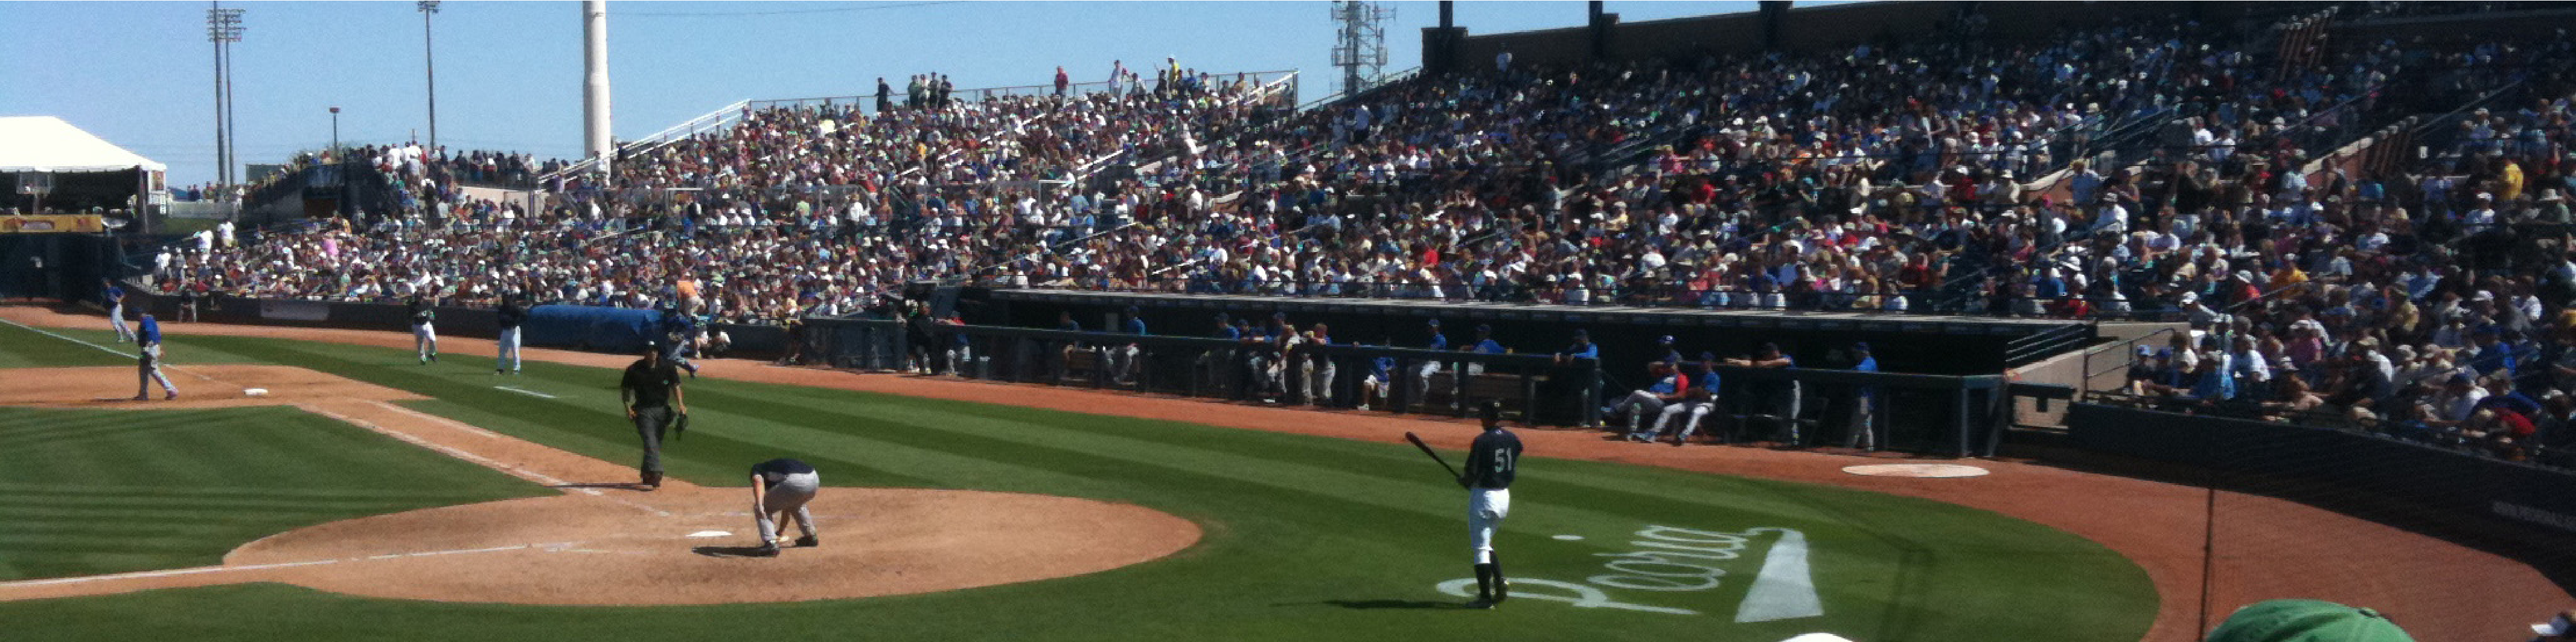
\includegraphics[width=\textwidth]{sampleteaser}
%   \caption{Seattle Mariners at Spring Training, 2010.}
%   \Description{Enjoying the baseball game from the third-base
%     seats. Ichiro Suzuki preparing to bat.}
%   \label{fig:teaser}
% \end{teaserfigure}

%%
%% This command processes the author and affiliation and title
%% information and builds the first part of the formatted document.
\maketitle

\section{Introduction} % Open

The adversarial robustness from the perspective of attack and defenses had been widely studied in recent research~\todo{cite}. However, most of these works analyzed graphs with less then 20,000 nodes. In particular from the perspective of real-world citation networks or internet-scale applications those graphs are tiny. In this work, we set the foundation for the study of adversarial robustness of GNNs on real-world citation/social networks. Importantly, it is unknown how the adversarial robustness/vulnerability relates to the graph size. Our first, experiments show that the adversarial robustness of a GNN depends on the graph size.

We show that contemporary surrogate losses are problematic for global attacks on large graphs. Especially in combination with realistic budgets, previous surrogate losses lead to weak attacks. We propose two new surrogate losses to overcome these limitations. On the traditional graphs, the new losses easily improve the strength of the attack by 33\% and for larger datasets we observe gains of more than 100\%. Hence, GNNs are even more fragile than previously believed.

Attacks based on combinatorial approaches easily become computationally infeasible because of the vast amount of potential adjacency matrices (\(2^{n^2}\)). With first-order optimization we can approximate the discrete optimization problem. First-order optimization attacks typically require the gradient towards the entries in the adjacency matrix and, hence, reduce the complexity to \(\Theta(n^2)\). To attack a small dataset such as PubMed (19,717 nodes), typically more than 20~GB are required if using a dense adjacency matrix. We argue that such memory requirements are still impractical and hinder practitioners to assess adversarial robustness. We identify the necessity to research scalable attacks for GNNs, due to the lack of such attacks for real-world graphs We propose two strategies how one may apply first-order optimization, without the burden of a dense adjacency matrix. In Section~\ref{sec:prbcd}, we describe how one might add/remove edges between existing nodes based on Randomized Block Coordinate Descent (R-BCD). Thereafter in Section~\ref{sec:attackkdd} we propose an attack that adds adversarial nodes and was one of the top 5 attacks of the KDD Cup 2020~\citep{Biendata2020}. In this work, we focus on the important task of node classification. Since we cover the task of global attacks our attacks can easily be generalized to graph classification.

The recent defense of~\citet{Geisler2020}, based on robust aggregations in the message passing step showed supervisor performance over the other compared defenses. We use the very recent advancements in differential sorting~\todo{cite}, to propose a computationally less demanding robust, differentiable aggregations. We call this aggregation Soft Median, observe a similar robustness to~\citep{Geisler2020} and can leverage the lower memory footprint in GNNs when memory is at premium.

Our contributions are the following:
\begin{itemize}
  \item We show that the widely used cross entropy is not a good surrogate loss for attacking the graph structure on graph neural networks.
  \item We propose two novel losses for global attacks on graph neural networks that overcome the limitations and empirically boosts the attack strength by up to 100\%.
  \item We propose two scalable adversarial attacks that add/remove edges between the existing nodes. One relies on projected gradient descent and the other uses a greedy FGSM-like optimization scheme (space complexity of \(\Theta(m)\) in the number of edges \(m\)).
  \item We propose one scalable adversarial attack that adds adversarial nodes (space complexity of \(\Theta(n)\)).
  \item We propose a differentiable robust aggregation that scales linearity w.r.t.\ the neighborhood size of the message passing aggregation and performs au par to the previous defense. This enables us to defend a GNN when memory is at premium.
  \item We study the adversarial robustness on graphs substantially larger than PubMed. Empirically, we find that the graph size negatively related to the adversarial robustness.
\end{itemize}

\section{Cross Entropy is a Bad Surrogate}\label{sec:ceisbad} % Simon

In the context of images, typically a single sample is attacked. In the context of graph neural networks this corresponds to a local attack. For such a scenario an untargeted attack it is often sufficient to maximize the cross entropy 
\begin{equation}\label{eq:crossentropy}
\text{CE}^{(n)}(y, \vp) = \sum_{c \in \sC} \mathbb{I}[y^{(n)} = c] \log(\evp_{c})^{(n)} = \log(\evp_{c^*}^{(n)})\,.
\end{equation}
Many \emph{global} attacks~\citep{Chen2018, Wu2019, Xu2018, Zugner2019a} also perform a global attack on a GNN via maximizing the cross entropy \(\max_{\adj} \text{CE}(f_{\theta}(\adj, \features))\). However, in our experiments, especially on large graphs, we have often observed that the CE loss increased while the accuracy did not decline. This can be explained by a bias of CE towards nodes which had a low confidence score (misclassified). Maximizing the CE is equivalent to minimizing the data likelihood and poorly correlates with the accuracy given this limited budget. This is apparent in Figure~\ref{fig:negceprob}.

\begin{figure}[t]
  \centering
  \makebox[\linewidth][c]{
    \(\begin{array}{cc}
      \subfloat[Clean graph]{\resizebox{0.5\linewidth}{!}{%% Creator: Matplotlib, PGF backend
%%
%% To include the figure in your LaTeX document, write
%%   \input{<filename>.pgf}
%%
%% Make sure the required packages are loaded in your preamble
%%   \usepackage{pgf}
%%
%% and, on pdftex
%%   \usepackage[utf8]{inputenc}\DeclareUnicodeCharacter{2212}{-}
%%
%% or, on luatex and xetex
%%   \usepackage{unicode-math}
%%
%% Figures using additional raster images can only be included by \input if
%% they are in the same directory as the main LaTeX file. For loading figures
%% from other directories you can use the `import` package
%%   \usepackage{import}
%%
%% and then include the figures with
%%   \import{<path to file>}{<filename>.pgf}
%%
%% Matplotlib used the following preamble
%%   \usepackage[utf8]{inputenc}
%%   \usepackage[T1]{fontenc}
%%   \usepackage{amsmath}
%%   \newcommand*{\mat}[1]{\boldsymbol{#1}}
%%
\begingroup%
\makeatletter%
\begin{pgfpicture}%
\pgfpathrectangle{\pgfpointorigin}{\pgfqpoint{10.063632in}{9.626613in}}%
\pgfusepath{use as bounding box, clip}%
\begin{pgfscope}%
\pgfsetbuttcap%
\pgfsetmiterjoin%
\definecolor{currentfill}{rgb}{1.000000,1.000000,1.000000}%
\pgfsetfillcolor{currentfill}%
\pgfsetlinewidth{0.000000pt}%
\definecolor{currentstroke}{rgb}{1.000000,1.000000,1.000000}%
\pgfsetstrokecolor{currentstroke}%
\pgfsetstrokeopacity{0.000000}%
\pgfsetdash{}{0pt}%
\pgfpathmoveto{\pgfqpoint{0.000000in}{0.000000in}}%
\pgfpathlineto{\pgfqpoint{10.063632in}{0.000000in}}%
\pgfpathlineto{\pgfqpoint{10.063632in}{9.626613in}}%
\pgfpathlineto{\pgfqpoint{0.000000in}{9.626613in}}%
\pgfpathclose%
\pgfusepath{fill}%
\end{pgfscope}%
\begin{pgfscope}%
\pgfsetbuttcap%
\pgfsetmiterjoin%
\definecolor{currentfill}{rgb}{1.000000,1.000000,1.000000}%
\pgfsetfillcolor{currentfill}%
\pgfsetlinewidth{0.000000pt}%
\definecolor{currentstroke}{rgb}{0.000000,0.000000,0.000000}%
\pgfsetstrokecolor{currentstroke}%
\pgfsetstrokeopacity{0.000000}%
\pgfsetdash{}{0pt}%
\pgfpathmoveto{\pgfqpoint{0.663632in}{0.466613in}}%
\pgfpathlineto{\pgfqpoint{9.963632in}{0.466613in}}%
\pgfpathlineto{\pgfqpoint{9.963632in}{9.526613in}}%
\pgfpathlineto{\pgfqpoint{0.663632in}{9.526613in}}%
\pgfpathclose%
\pgfusepath{fill}%
\end{pgfscope}%
\begin{pgfscope}%
\pgfpathrectangle{\pgfqpoint{0.663632in}{0.466613in}}{\pgfqpoint{9.300000in}{9.060000in}}%
\pgfusepath{clip}%
\pgfsetroundcap%
\pgfsetroundjoin%
\pgfsetlinewidth{0.501875pt}%
\definecolor{currentstroke}{rgb}{0.800000,0.800000,0.800000}%
\pgfsetstrokecolor{currentstroke}%
\pgfsetdash{}{0pt}%
\pgfpathmoveto{\pgfqpoint{1.086359in}{0.466613in}}%
\pgfpathlineto{\pgfqpoint{1.086359in}{9.526613in}}%
\pgfusepath{stroke}%
\end{pgfscope}%
\begin{pgfscope}%
\definecolor{textcolor}{rgb}{0.150000,0.150000,0.150000}%
\pgfsetstrokecolor{textcolor}%
\pgfsetfillcolor{textcolor}%
\pgftext[x=1.086359in,y=0.376335in,,top]{\color{textcolor}\rmfamily\fontsize{8.000000}{9.600000}\selectfont \(\displaystyle {0.0}\)}%
\end{pgfscope}%
\begin{pgfscope}%
\pgfpathrectangle{\pgfqpoint{0.663632in}{0.466613in}}{\pgfqpoint{9.300000in}{9.060000in}}%
\pgfusepath{clip}%
\pgfsetroundcap%
\pgfsetroundjoin%
\pgfsetlinewidth{0.501875pt}%
\definecolor{currentstroke}{rgb}{0.800000,0.800000,0.800000}%
\pgfsetstrokecolor{currentstroke}%
\pgfsetdash{}{0pt}%
\pgfpathmoveto{\pgfqpoint{2.777269in}{0.466613in}}%
\pgfpathlineto{\pgfqpoint{2.777269in}{9.526613in}}%
\pgfusepath{stroke}%
\end{pgfscope}%
\begin{pgfscope}%
\definecolor{textcolor}{rgb}{0.150000,0.150000,0.150000}%
\pgfsetstrokecolor{textcolor}%
\pgfsetfillcolor{textcolor}%
\pgftext[x=2.777269in,y=0.376335in,,top]{\color{textcolor}\rmfamily\fontsize{8.000000}{9.600000}\selectfont \(\displaystyle {0.2}\)}%
\end{pgfscope}%
\begin{pgfscope}%
\pgfpathrectangle{\pgfqpoint{0.663632in}{0.466613in}}{\pgfqpoint{9.300000in}{9.060000in}}%
\pgfusepath{clip}%
\pgfsetroundcap%
\pgfsetroundjoin%
\pgfsetlinewidth{0.501875pt}%
\definecolor{currentstroke}{rgb}{0.800000,0.800000,0.800000}%
\pgfsetstrokecolor{currentstroke}%
\pgfsetdash{}{0pt}%
\pgfpathmoveto{\pgfqpoint{4.468180in}{0.466613in}}%
\pgfpathlineto{\pgfqpoint{4.468180in}{9.526613in}}%
\pgfusepath{stroke}%
\end{pgfscope}%
\begin{pgfscope}%
\definecolor{textcolor}{rgb}{0.150000,0.150000,0.150000}%
\pgfsetstrokecolor{textcolor}%
\pgfsetfillcolor{textcolor}%
\pgftext[x=4.468180in,y=0.376335in,,top]{\color{textcolor}\rmfamily\fontsize{8.000000}{9.600000}\selectfont \(\displaystyle {0.4}\)}%
\end{pgfscope}%
\begin{pgfscope}%
\pgfpathrectangle{\pgfqpoint{0.663632in}{0.466613in}}{\pgfqpoint{9.300000in}{9.060000in}}%
\pgfusepath{clip}%
\pgfsetroundcap%
\pgfsetroundjoin%
\pgfsetlinewidth{0.501875pt}%
\definecolor{currentstroke}{rgb}{0.800000,0.800000,0.800000}%
\pgfsetstrokecolor{currentstroke}%
\pgfsetdash{}{0pt}%
\pgfpathmoveto{\pgfqpoint{6.159091in}{0.466613in}}%
\pgfpathlineto{\pgfqpoint{6.159091in}{9.526613in}}%
\pgfusepath{stroke}%
\end{pgfscope}%
\begin{pgfscope}%
\definecolor{textcolor}{rgb}{0.150000,0.150000,0.150000}%
\pgfsetstrokecolor{textcolor}%
\pgfsetfillcolor{textcolor}%
\pgftext[x=6.159091in,y=0.376335in,,top]{\color{textcolor}\rmfamily\fontsize{8.000000}{9.600000}\selectfont \(\displaystyle {0.6}\)}%
\end{pgfscope}%
\begin{pgfscope}%
\pgfpathrectangle{\pgfqpoint{0.663632in}{0.466613in}}{\pgfqpoint{9.300000in}{9.060000in}}%
\pgfusepath{clip}%
\pgfsetroundcap%
\pgfsetroundjoin%
\pgfsetlinewidth{0.501875pt}%
\definecolor{currentstroke}{rgb}{0.800000,0.800000,0.800000}%
\pgfsetstrokecolor{currentstroke}%
\pgfsetdash{}{0pt}%
\pgfpathmoveto{\pgfqpoint{7.850001in}{0.466613in}}%
\pgfpathlineto{\pgfqpoint{7.850001in}{9.526613in}}%
\pgfusepath{stroke}%
\end{pgfscope}%
\begin{pgfscope}%
\definecolor{textcolor}{rgb}{0.150000,0.150000,0.150000}%
\pgfsetstrokecolor{textcolor}%
\pgfsetfillcolor{textcolor}%
\pgftext[x=7.850001in,y=0.376335in,,top]{\color{textcolor}\rmfamily\fontsize{8.000000}{9.600000}\selectfont \(\displaystyle {0.8}\)}%
\end{pgfscope}%
\begin{pgfscope}%
\pgfpathrectangle{\pgfqpoint{0.663632in}{0.466613in}}{\pgfqpoint{9.300000in}{9.060000in}}%
\pgfusepath{clip}%
\pgfsetroundcap%
\pgfsetroundjoin%
\pgfsetlinewidth{0.501875pt}%
\definecolor{currentstroke}{rgb}{0.800000,0.800000,0.800000}%
\pgfsetstrokecolor{currentstroke}%
\pgfsetdash{}{0pt}%
\pgfpathmoveto{\pgfqpoint{9.540912in}{0.466613in}}%
\pgfpathlineto{\pgfqpoint{9.540912in}{9.526613in}}%
\pgfusepath{stroke}%
\end{pgfscope}%
\begin{pgfscope}%
\definecolor{textcolor}{rgb}{0.150000,0.150000,0.150000}%
\pgfsetstrokecolor{textcolor}%
\pgfsetfillcolor{textcolor}%
\pgftext[x=9.540912in,y=0.376335in,,top]{\color{textcolor}\rmfamily\fontsize{8.000000}{9.600000}\selectfont \(\displaystyle {1.0}\)}%
\end{pgfscope}%
\begin{pgfscope}%
\definecolor{textcolor}{rgb}{0.150000,0.150000,0.150000}%
\pgfsetstrokecolor{textcolor}%
\pgfsetfillcolor{textcolor}%
\pgftext[x=5.313632in,y=0.222655in,,top]{\color{textcolor}\rmfamily\fontsize{10.000000}{12.000000}\selectfont Probability of attacked node}%
\end{pgfscope}%
\begin{pgfscope}%
\pgfpathrectangle{\pgfqpoint{0.663632in}{0.466613in}}{\pgfqpoint{9.300000in}{9.060000in}}%
\pgfusepath{clip}%
\pgfsetroundcap%
\pgfsetroundjoin%
\pgfsetlinewidth{0.501875pt}%
\definecolor{currentstroke}{rgb}{0.800000,0.800000,0.800000}%
\pgfsetstrokecolor{currentstroke}%
\pgfsetdash{}{0pt}%
\pgfpathmoveto{\pgfqpoint{0.663632in}{0.466613in}}%
\pgfpathlineto{\pgfqpoint{9.963632in}{0.466613in}}%
\pgfusepath{stroke}%
\end{pgfscope}%
\begin{pgfscope}%
\definecolor{textcolor}{rgb}{0.150000,0.150000,0.150000}%
\pgfsetstrokecolor{textcolor}%
\pgfsetfillcolor{textcolor}%
\pgftext[x=0.514325in, y=0.428350in, left, base]{\color{textcolor}\rmfamily\fontsize{8.000000}{9.600000}\selectfont \(\displaystyle {0}\)}%
\end{pgfscope}%
\begin{pgfscope}%
\pgfpathrectangle{\pgfqpoint{0.663632in}{0.466613in}}{\pgfqpoint{9.300000in}{9.060000in}}%
\pgfusepath{clip}%
\pgfsetroundcap%
\pgfsetroundjoin%
\pgfsetlinewidth{0.501875pt}%
\definecolor{currentstroke}{rgb}{0.800000,0.800000,0.800000}%
\pgfsetstrokecolor{currentstroke}%
\pgfsetdash{}{0pt}%
\pgfpathmoveto{\pgfqpoint{0.663632in}{1.886837in}}%
\pgfpathlineto{\pgfqpoint{9.963632in}{1.886837in}}%
\pgfusepath{stroke}%
\end{pgfscope}%
\begin{pgfscope}%
\definecolor{textcolor}{rgb}{0.150000,0.150000,0.150000}%
\pgfsetstrokecolor{textcolor}%
\pgfsetfillcolor{textcolor}%
\pgftext[x=0.337239in, y=1.848575in, left, base]{\color{textcolor}\rmfamily\fontsize{8.000000}{9.600000}\selectfont \(\displaystyle {2000}\)}%
\end{pgfscope}%
\begin{pgfscope}%
\pgfpathrectangle{\pgfqpoint{0.663632in}{0.466613in}}{\pgfqpoint{9.300000in}{9.060000in}}%
\pgfusepath{clip}%
\pgfsetroundcap%
\pgfsetroundjoin%
\pgfsetlinewidth{0.501875pt}%
\definecolor{currentstroke}{rgb}{0.800000,0.800000,0.800000}%
\pgfsetstrokecolor{currentstroke}%
\pgfsetdash{}{0pt}%
\pgfpathmoveto{\pgfqpoint{0.663632in}{3.307061in}}%
\pgfpathlineto{\pgfqpoint{9.963632in}{3.307061in}}%
\pgfusepath{stroke}%
\end{pgfscope}%
\begin{pgfscope}%
\definecolor{textcolor}{rgb}{0.150000,0.150000,0.150000}%
\pgfsetstrokecolor{textcolor}%
\pgfsetfillcolor{textcolor}%
\pgftext[x=0.337239in, y=3.268799in, left, base]{\color{textcolor}\rmfamily\fontsize{8.000000}{9.600000}\selectfont \(\displaystyle {4000}\)}%
\end{pgfscope}%
\begin{pgfscope}%
\pgfpathrectangle{\pgfqpoint{0.663632in}{0.466613in}}{\pgfqpoint{9.300000in}{9.060000in}}%
\pgfusepath{clip}%
\pgfsetroundcap%
\pgfsetroundjoin%
\pgfsetlinewidth{0.501875pt}%
\definecolor{currentstroke}{rgb}{0.800000,0.800000,0.800000}%
\pgfsetstrokecolor{currentstroke}%
\pgfsetdash{}{0pt}%
\pgfpathmoveto{\pgfqpoint{0.663632in}{4.727285in}}%
\pgfpathlineto{\pgfqpoint{9.963632in}{4.727285in}}%
\pgfusepath{stroke}%
\end{pgfscope}%
\begin{pgfscope}%
\definecolor{textcolor}{rgb}{0.150000,0.150000,0.150000}%
\pgfsetstrokecolor{textcolor}%
\pgfsetfillcolor{textcolor}%
\pgftext[x=0.337239in, y=4.689023in, left, base]{\color{textcolor}\rmfamily\fontsize{8.000000}{9.600000}\selectfont \(\displaystyle {6000}\)}%
\end{pgfscope}%
\begin{pgfscope}%
\pgfpathrectangle{\pgfqpoint{0.663632in}{0.466613in}}{\pgfqpoint{9.300000in}{9.060000in}}%
\pgfusepath{clip}%
\pgfsetroundcap%
\pgfsetroundjoin%
\pgfsetlinewidth{0.501875pt}%
\definecolor{currentstroke}{rgb}{0.800000,0.800000,0.800000}%
\pgfsetstrokecolor{currentstroke}%
\pgfsetdash{}{0pt}%
\pgfpathmoveto{\pgfqpoint{0.663632in}{6.147509in}}%
\pgfpathlineto{\pgfqpoint{9.963632in}{6.147509in}}%
\pgfusepath{stroke}%
\end{pgfscope}%
\begin{pgfscope}%
\definecolor{textcolor}{rgb}{0.150000,0.150000,0.150000}%
\pgfsetstrokecolor{textcolor}%
\pgfsetfillcolor{textcolor}%
\pgftext[x=0.337239in, y=6.109247in, left, base]{\color{textcolor}\rmfamily\fontsize{8.000000}{9.600000}\selectfont \(\displaystyle {8000}\)}%
\end{pgfscope}%
\begin{pgfscope}%
\pgfpathrectangle{\pgfqpoint{0.663632in}{0.466613in}}{\pgfqpoint{9.300000in}{9.060000in}}%
\pgfusepath{clip}%
\pgfsetroundcap%
\pgfsetroundjoin%
\pgfsetlinewidth{0.501875pt}%
\definecolor{currentstroke}{rgb}{0.800000,0.800000,0.800000}%
\pgfsetstrokecolor{currentstroke}%
\pgfsetdash{}{0pt}%
\pgfpathmoveto{\pgfqpoint{0.663632in}{7.567733in}}%
\pgfpathlineto{\pgfqpoint{9.963632in}{7.567733in}}%
\pgfusepath{stroke}%
\end{pgfscope}%
\begin{pgfscope}%
\definecolor{textcolor}{rgb}{0.150000,0.150000,0.150000}%
\pgfsetstrokecolor{textcolor}%
\pgfsetfillcolor{textcolor}%
\pgftext[x=0.278211in, y=7.529471in, left, base]{\color{textcolor}\rmfamily\fontsize{8.000000}{9.600000}\selectfont \(\displaystyle {10000}\)}%
\end{pgfscope}%
\begin{pgfscope}%
\pgfpathrectangle{\pgfqpoint{0.663632in}{0.466613in}}{\pgfqpoint{9.300000in}{9.060000in}}%
\pgfusepath{clip}%
\pgfsetroundcap%
\pgfsetroundjoin%
\pgfsetlinewidth{0.501875pt}%
\definecolor{currentstroke}{rgb}{0.800000,0.800000,0.800000}%
\pgfsetstrokecolor{currentstroke}%
\pgfsetdash{}{0pt}%
\pgfpathmoveto{\pgfqpoint{0.663632in}{8.987957in}}%
\pgfpathlineto{\pgfqpoint{9.963632in}{8.987957in}}%
\pgfusepath{stroke}%
\end{pgfscope}%
\begin{pgfscope}%
\definecolor{textcolor}{rgb}{0.150000,0.150000,0.150000}%
\pgfsetstrokecolor{textcolor}%
\pgfsetfillcolor{textcolor}%
\pgftext[x=0.278211in, y=8.949695in, left, base]{\color{textcolor}\rmfamily\fontsize{8.000000}{9.600000}\selectfont \(\displaystyle {12000}\)}%
\end{pgfscope}%
\begin{pgfscope}%
\definecolor{textcolor}{rgb}{0.150000,0.150000,0.150000}%
\pgfsetstrokecolor{textcolor}%
\pgfsetfillcolor{textcolor}%
\pgftext[x=0.222655in,y=4.996613in,,bottom,rotate=90.000000]{\color{textcolor}\rmfamily\fontsize{10.000000}{12.000000}\selectfont Probability density}%
\end{pgfscope}%
\begin{pgfscope}%
\pgfpathrectangle{\pgfqpoint{0.663632in}{0.466613in}}{\pgfqpoint{9.300000in}{9.060000in}}%
\pgfusepath{clip}%
\pgfsetbuttcap%
\pgfsetmiterjoin%
\definecolor{currentfill}{rgb}{0.298039,0.447059,0.690196}%
\pgfsetfillcolor{currentfill}%
\pgfsetlinewidth{1.003750pt}%
\definecolor{currentstroke}{rgb}{1.000000,1.000000,1.000000}%
\pgfsetstrokecolor{currentstroke}%
\pgfsetdash{}{0pt}%
\pgfpathmoveto{\pgfqpoint{1.086359in}{0.466613in}}%
\pgfpathlineto{\pgfqpoint{1.931813in}{0.466613in}}%
\pgfpathlineto{\pgfqpoint{1.931813in}{4.958071in}}%
\pgfpathlineto{\pgfqpoint{1.086359in}{4.958071in}}%
\pgfpathclose%
\pgfusepath{stroke,fill}%
\end{pgfscope}%
\begin{pgfscope}%
\pgfpathrectangle{\pgfqpoint{0.663632in}{0.466613in}}{\pgfqpoint{9.300000in}{9.060000in}}%
\pgfusepath{clip}%
\pgfsetbuttcap%
\pgfsetmiterjoin%
\definecolor{currentfill}{rgb}{0.298039,0.447059,0.690196}%
\pgfsetfillcolor{currentfill}%
\pgfsetlinewidth{1.003750pt}%
\definecolor{currentstroke}{rgb}{1.000000,1.000000,1.000000}%
\pgfsetstrokecolor{currentstroke}%
\pgfsetdash{}{0pt}%
\pgfpathmoveto{\pgfqpoint{1.931813in}{0.466613in}}%
\pgfpathlineto{\pgfqpoint{2.777268in}{0.466613in}}%
\pgfpathlineto{\pgfqpoint{2.777268in}{2.986800in}}%
\pgfpathlineto{\pgfqpoint{1.931813in}{2.986800in}}%
\pgfpathclose%
\pgfusepath{stroke,fill}%
\end{pgfscope}%
\begin{pgfscope}%
\pgfpathrectangle{\pgfqpoint{0.663632in}{0.466613in}}{\pgfqpoint{9.300000in}{9.060000in}}%
\pgfusepath{clip}%
\pgfsetbuttcap%
\pgfsetmiterjoin%
\definecolor{currentfill}{rgb}{0.298039,0.447059,0.690196}%
\pgfsetfillcolor{currentfill}%
\pgfsetlinewidth{1.003750pt}%
\definecolor{currentstroke}{rgb}{1.000000,1.000000,1.000000}%
\pgfsetstrokecolor{currentstroke}%
\pgfsetdash{}{0pt}%
\pgfpathmoveto{\pgfqpoint{2.777268in}{0.466613in}}%
\pgfpathlineto{\pgfqpoint{3.622723in}{0.466613in}}%
\pgfpathlineto{\pgfqpoint{3.622723in}{2.903717in}}%
\pgfpathlineto{\pgfqpoint{2.777268in}{2.903717in}}%
\pgfpathclose%
\pgfusepath{stroke,fill}%
\end{pgfscope}%
\begin{pgfscope}%
\pgfpathrectangle{\pgfqpoint{0.663632in}{0.466613in}}{\pgfqpoint{9.300000in}{9.060000in}}%
\pgfusepath{clip}%
\pgfsetbuttcap%
\pgfsetmiterjoin%
\definecolor{currentfill}{rgb}{0.298039,0.447059,0.690196}%
\pgfsetfillcolor{currentfill}%
\pgfsetlinewidth{1.003750pt}%
\definecolor{currentstroke}{rgb}{1.000000,1.000000,1.000000}%
\pgfsetstrokecolor{currentstroke}%
\pgfsetdash{}{0pt}%
\pgfpathmoveto{\pgfqpoint{3.622722in}{0.466613in}}%
\pgfpathlineto{\pgfqpoint{4.468177in}{0.466613in}}%
\pgfpathlineto{\pgfqpoint{4.468177in}{2.853299in}}%
\pgfpathlineto{\pgfqpoint{3.622722in}{2.853299in}}%
\pgfpathclose%
\pgfusepath{stroke,fill}%
\end{pgfscope}%
\begin{pgfscope}%
\pgfpathrectangle{\pgfqpoint{0.663632in}{0.466613in}}{\pgfqpoint{9.300000in}{9.060000in}}%
\pgfusepath{clip}%
\pgfsetbuttcap%
\pgfsetmiterjoin%
\definecolor{currentfill}{rgb}{0.298039,0.447059,0.690196}%
\pgfsetfillcolor{currentfill}%
\pgfsetlinewidth{1.003750pt}%
\definecolor{currentstroke}{rgb}{1.000000,1.000000,1.000000}%
\pgfsetstrokecolor{currentstroke}%
\pgfsetdash{}{0pt}%
\pgfpathmoveto{\pgfqpoint{4.468177in}{0.466613in}}%
\pgfpathlineto{\pgfqpoint{5.313631in}{0.466613in}}%
\pgfpathlineto{\pgfqpoint{5.313631in}{2.920050in}}%
\pgfpathlineto{\pgfqpoint{4.468177in}{2.920050in}}%
\pgfpathclose%
\pgfusepath{stroke,fill}%
\end{pgfscope}%
\begin{pgfscope}%
\pgfpathrectangle{\pgfqpoint{0.663632in}{0.466613in}}{\pgfqpoint{9.300000in}{9.060000in}}%
\pgfusepath{clip}%
\pgfsetbuttcap%
\pgfsetmiterjoin%
\definecolor{currentfill}{rgb}{0.298039,0.447059,0.690196}%
\pgfsetfillcolor{currentfill}%
\pgfsetlinewidth{1.003750pt}%
\definecolor{currentstroke}{rgb}{1.000000,1.000000,1.000000}%
\pgfsetstrokecolor{currentstroke}%
\pgfsetdash{}{0pt}%
\pgfpathmoveto{\pgfqpoint{5.313632in}{0.466613in}}%
\pgfpathlineto{\pgfqpoint{6.159087in}{0.466613in}}%
\pgfpathlineto{\pgfqpoint{6.159087in}{2.888095in}}%
\pgfpathlineto{\pgfqpoint{5.313632in}{2.888095in}}%
\pgfpathclose%
\pgfusepath{stroke,fill}%
\end{pgfscope}%
\begin{pgfscope}%
\pgfpathrectangle{\pgfqpoint{0.663632in}{0.466613in}}{\pgfqpoint{9.300000in}{9.060000in}}%
\pgfusepath{clip}%
\pgfsetbuttcap%
\pgfsetmiterjoin%
\definecolor{currentfill}{rgb}{0.298039,0.447059,0.690196}%
\pgfsetfillcolor{currentfill}%
\pgfsetlinewidth{1.003750pt}%
\definecolor{currentstroke}{rgb}{1.000000,1.000000,1.000000}%
\pgfsetstrokecolor{currentstroke}%
\pgfsetdash{}{0pt}%
\pgfpathmoveto{\pgfqpoint{6.159086in}{0.466613in}}%
\pgfpathlineto{\pgfqpoint{7.004541in}{0.466613in}}%
\pgfpathlineto{\pgfqpoint{7.004541in}{2.919340in}}%
\pgfpathlineto{\pgfqpoint{6.159086in}{2.919340in}}%
\pgfpathclose%
\pgfusepath{stroke,fill}%
\end{pgfscope}%
\begin{pgfscope}%
\pgfpathrectangle{\pgfqpoint{0.663632in}{0.466613in}}{\pgfqpoint{9.300000in}{9.060000in}}%
\pgfusepath{clip}%
\pgfsetbuttcap%
\pgfsetmiterjoin%
\definecolor{currentfill}{rgb}{0.298039,0.447059,0.690196}%
\pgfsetfillcolor{currentfill}%
\pgfsetlinewidth{1.003750pt}%
\definecolor{currentstroke}{rgb}{1.000000,1.000000,1.000000}%
\pgfsetstrokecolor{currentstroke}%
\pgfsetdash{}{0pt}%
\pgfpathmoveto{\pgfqpoint{7.004541in}{0.466613in}}%
\pgfpathlineto{\pgfqpoint{7.849995in}{0.466613in}}%
\pgfpathlineto{\pgfqpoint{7.849995in}{3.255933in}}%
\pgfpathlineto{\pgfqpoint{7.004541in}{3.255933in}}%
\pgfpathclose%
\pgfusepath{stroke,fill}%
\end{pgfscope}%
\begin{pgfscope}%
\pgfpathrectangle{\pgfqpoint{0.663632in}{0.466613in}}{\pgfqpoint{9.300000in}{9.060000in}}%
\pgfusepath{clip}%
\pgfsetbuttcap%
\pgfsetmiterjoin%
\definecolor{currentfill}{rgb}{0.298039,0.447059,0.690196}%
\pgfsetfillcolor{currentfill}%
\pgfsetlinewidth{1.003750pt}%
\definecolor{currentstroke}{rgb}{1.000000,1.000000,1.000000}%
\pgfsetstrokecolor{currentstroke}%
\pgfsetdash{}{0pt}%
\pgfpathmoveto{\pgfqpoint{7.849995in}{0.466613in}}%
\pgfpathlineto{\pgfqpoint{8.695450in}{0.466613in}}%
\pgfpathlineto{\pgfqpoint{8.695450in}{4.399213in}}%
\pgfpathlineto{\pgfqpoint{7.849995in}{4.399213in}}%
\pgfpathclose%
\pgfusepath{stroke,fill}%
\end{pgfscope}%
\begin{pgfscope}%
\pgfpathrectangle{\pgfqpoint{0.663632in}{0.466613in}}{\pgfqpoint{9.300000in}{9.060000in}}%
\pgfusepath{clip}%
\pgfsetbuttcap%
\pgfsetmiterjoin%
\definecolor{currentfill}{rgb}{0.298039,0.447059,0.690196}%
\pgfsetfillcolor{currentfill}%
\pgfsetlinewidth{1.003750pt}%
\definecolor{currentstroke}{rgb}{1.000000,1.000000,1.000000}%
\pgfsetstrokecolor{currentstroke}%
\pgfsetdash{}{0pt}%
\pgfpathmoveto{\pgfqpoint{8.695450in}{0.466613in}}%
\pgfpathlineto{\pgfqpoint{9.540904in}{0.466613in}}%
\pgfpathlineto{\pgfqpoint{9.540904in}{9.095184in}}%
\pgfpathlineto{\pgfqpoint{8.695450in}{9.095184in}}%
\pgfpathclose%
\pgfusepath{stroke,fill}%
\end{pgfscope}%
\begin{pgfscope}%
\pgfsetrectcap%
\pgfsetmiterjoin%
\pgfsetlinewidth{0.752812pt}%
\definecolor{currentstroke}{rgb}{0.700000,0.700000,0.700000}%
\pgfsetstrokecolor{currentstroke}%
\pgfsetdash{}{0pt}%
\pgfpathmoveto{\pgfqpoint{0.663632in}{0.466613in}}%
\pgfpathlineto{\pgfqpoint{0.663632in}{9.526613in}}%
\pgfusepath{stroke}%
\end{pgfscope}%
\begin{pgfscope}%
\pgfsetrectcap%
\pgfsetmiterjoin%
\pgfsetlinewidth{0.752812pt}%
\definecolor{currentstroke}{rgb}{0.700000,0.700000,0.700000}%
\pgfsetstrokecolor{currentstroke}%
\pgfsetdash{}{0pt}%
\pgfpathmoveto{\pgfqpoint{9.963632in}{0.466613in}}%
\pgfpathlineto{\pgfqpoint{9.963632in}{9.526613in}}%
\pgfusepath{stroke}%
\end{pgfscope}%
\begin{pgfscope}%
\pgfsetrectcap%
\pgfsetmiterjoin%
\pgfsetlinewidth{0.752812pt}%
\definecolor{currentstroke}{rgb}{0.700000,0.700000,0.700000}%
\pgfsetstrokecolor{currentstroke}%
\pgfsetdash{}{0pt}%
\pgfpathmoveto{\pgfqpoint{0.663632in}{0.466613in}}%
\pgfpathlineto{\pgfqpoint{9.963632in}{0.466613in}}%
\pgfusepath{stroke}%
\end{pgfscope}%
\begin{pgfscope}%
\pgfsetrectcap%
\pgfsetmiterjoin%
\pgfsetlinewidth{0.752812pt}%
\definecolor{currentstroke}{rgb}{0.700000,0.700000,0.700000}%
\pgfsetstrokecolor{currentstroke}%
\pgfsetdash{}{0pt}%
\pgfpathmoveto{\pgfqpoint{0.663632in}{9.526613in}}%
\pgfpathlineto{\pgfqpoint{9.963632in}{9.526613in}}%
\pgfusepath{stroke}%
\end{pgfscope}%
\end{pgfpicture}%
\makeatother%
\endgroup%
}} &
      \subfloat[Attacked nodes]{\resizebox{0.5\linewidth}{!}{%% Creator: Matplotlib, PGF backend
%%
%% To include the figure in your LaTeX document, write
%%   \input{<filename>.pgf}
%%
%% Make sure the required packages are loaded in your preamble
%%   \usepackage{pgf}
%%
%% and, on pdftex
%%   \usepackage[utf8]{inputenc}\DeclareUnicodeCharacter{2212}{-}
%%
%% or, on luatex and xetex
%%   \usepackage{unicode-math}
%%
%% Figures using additional raster images can only be included by \input if
%% they are in the same directory as the main LaTeX file. For loading figures
%% from other directories you can use the `import` package
%%   \usepackage{import}
%%
%% and then include the figures with
%%   \import{<path to file>}{<filename>.pgf}
%%
%% Matplotlib used the following preamble
%%   \usepackage[utf8]{inputenc}
%%   \usepackage[T1]{fontenc}
%%   \usepackage{amsmath}
%%   \newcommand*{\mat}[1]{\boldsymbol{#1}}
%%
\begingroup%
\makeatletter%
\begin{pgfpicture}%
\pgfpathrectangle{\pgfpointorigin}{\pgfqpoint{2.000721in}{1.819295in}}%
\pgfusepath{use as bounding box, clip}%
\begin{pgfscope}%
\pgfsetbuttcap%
\pgfsetmiterjoin%
\definecolor{currentfill}{rgb}{1.000000,1.000000,1.000000}%
\pgfsetfillcolor{currentfill}%
\pgfsetlinewidth{0.000000pt}%
\definecolor{currentstroke}{rgb}{1.000000,1.000000,1.000000}%
\pgfsetstrokecolor{currentstroke}%
\pgfsetstrokeopacity{0.000000}%
\pgfsetdash{}{0pt}%
\pgfpathmoveto{\pgfqpoint{-0.000000in}{0.000000in}}%
\pgfpathlineto{\pgfqpoint{2.000721in}{0.000000in}}%
\pgfpathlineto{\pgfqpoint{2.000721in}{1.819295in}}%
\pgfpathlineto{\pgfqpoint{-0.000000in}{1.819295in}}%
\pgfpathclose%
\pgfusepath{fill}%
\end{pgfscope}%
\begin{pgfscope}%
\pgfsetbuttcap%
\pgfsetmiterjoin%
\definecolor{currentfill}{rgb}{1.000000,1.000000,1.000000}%
\pgfsetfillcolor{currentfill}%
\pgfsetlinewidth{0.000000pt}%
\definecolor{currentstroke}{rgb}{0.000000,0.000000,0.000000}%
\pgfsetstrokecolor{currentstroke}%
\pgfsetstrokeopacity{0.000000}%
\pgfsetdash{}{0pt}%
\pgfpathmoveto{\pgfqpoint{0.604603in}{0.473545in}}%
\pgfpathlineto{\pgfqpoint{1.883353in}{0.473545in}}%
\pgfpathlineto{\pgfqpoint{1.883353in}{1.719295in}}%
\pgfpathlineto{\pgfqpoint{0.604603in}{1.719295in}}%
\pgfpathclose%
\pgfusepath{fill}%
\end{pgfscope}%
\begin{pgfscope}%
\pgfpathrectangle{\pgfqpoint{0.604603in}{0.473545in}}{\pgfqpoint{1.278750in}{1.245750in}}%
\pgfusepath{clip}%
\pgfsetroundcap%
\pgfsetroundjoin%
\pgfsetlinewidth{0.501875pt}%
\definecolor{currentstroke}{rgb}{0.800000,0.800000,0.800000}%
\pgfsetstrokecolor{currentstroke}%
\pgfsetdash{}{0pt}%
\pgfpathmoveto{\pgfqpoint{0.662728in}{0.473545in}}%
\pgfpathlineto{\pgfqpoint{0.662728in}{1.719295in}}%
\pgfusepath{stroke}%
\end{pgfscope}%
\begin{pgfscope}%
\definecolor{textcolor}{rgb}{0.150000,0.150000,0.150000}%
\pgfsetstrokecolor{textcolor}%
\pgfsetfillcolor{textcolor}%
\pgftext[x=0.662728in,y=0.383267in,,top]{\color{textcolor}\rmfamily\fontsize{8.000000}{9.600000}\selectfont \(\displaystyle {0.0}\)}%
\end{pgfscope}%
\begin{pgfscope}%
\pgfpathrectangle{\pgfqpoint{0.604603in}{0.473545in}}{\pgfqpoint{1.278750in}{1.245750in}}%
\pgfusepath{clip}%
\pgfsetroundcap%
\pgfsetroundjoin%
\pgfsetlinewidth{0.501875pt}%
\definecolor{currentstroke}{rgb}{0.800000,0.800000,0.800000}%
\pgfsetstrokecolor{currentstroke}%
\pgfsetdash{}{0pt}%
\pgfpathmoveto{\pgfqpoint{1.244012in}{0.473545in}}%
\pgfpathlineto{\pgfqpoint{1.244012in}{1.719295in}}%
\pgfusepath{stroke}%
\end{pgfscope}%
\begin{pgfscope}%
\definecolor{textcolor}{rgb}{0.150000,0.150000,0.150000}%
\pgfsetstrokecolor{textcolor}%
\pgfsetfillcolor{textcolor}%
\pgftext[x=1.244012in,y=0.383267in,,top]{\color{textcolor}\rmfamily\fontsize{8.000000}{9.600000}\selectfont \(\displaystyle {0.5}\)}%
\end{pgfscope}%
\begin{pgfscope}%
\pgfpathrectangle{\pgfqpoint{0.604603in}{0.473545in}}{\pgfqpoint{1.278750in}{1.245750in}}%
\pgfusepath{clip}%
\pgfsetroundcap%
\pgfsetroundjoin%
\pgfsetlinewidth{0.501875pt}%
\definecolor{currentstroke}{rgb}{0.800000,0.800000,0.800000}%
\pgfsetstrokecolor{currentstroke}%
\pgfsetdash{}{0pt}%
\pgfpathmoveto{\pgfqpoint{1.825296in}{0.473545in}}%
\pgfpathlineto{\pgfqpoint{1.825296in}{1.719295in}}%
\pgfusepath{stroke}%
\end{pgfscope}%
\begin{pgfscope}%
\definecolor{textcolor}{rgb}{0.150000,0.150000,0.150000}%
\pgfsetstrokecolor{textcolor}%
\pgfsetfillcolor{textcolor}%
\pgftext[x=1.825296in,y=0.383267in,,top]{\color{textcolor}\rmfamily\fontsize{8.000000}{9.600000}\selectfont \(\displaystyle {1.0}\)}%
\end{pgfscope}%
\begin{pgfscope}%
\definecolor{textcolor}{rgb}{0.150000,0.150000,0.150000}%
\pgfsetstrokecolor{textcolor}%
\pgfsetfillcolor{textcolor}%
\pgftext[x=1.243978in,y=0.229588in,,top]{\color{textcolor}\rmfamily\fontsize{10.000000}{12.000000}\selectfont Prob. score \(\displaystyle p^*\)}%
\end{pgfscope}%
\begin{pgfscope}%
\pgfpathrectangle{\pgfqpoint{0.604603in}{0.473545in}}{\pgfqpoint{1.278750in}{1.245750in}}%
\pgfusepath{clip}%
\pgfsetroundcap%
\pgfsetroundjoin%
\pgfsetlinewidth{0.501875pt}%
\definecolor{currentstroke}{rgb}{0.800000,0.800000,0.800000}%
\pgfsetstrokecolor{currentstroke}%
\pgfsetdash{}{0pt}%
\pgfpathmoveto{\pgfqpoint{0.604603in}{0.473545in}}%
\pgfpathlineto{\pgfqpoint{1.883353in}{0.473545in}}%
\pgfusepath{stroke}%
\end{pgfscope}%
\begin{pgfscope}%
\definecolor{textcolor}{rgb}{0.150000,0.150000,0.150000}%
\pgfsetstrokecolor{textcolor}%
\pgfsetfillcolor{textcolor}%
\pgftext[x=0.455297in, y=0.435283in, left, base]{\color{textcolor}\rmfamily\fontsize{8.000000}{9.600000}\selectfont \(\displaystyle {0}\)}%
\end{pgfscope}%
\begin{pgfscope}%
\pgfpathrectangle{\pgfqpoint{0.604603in}{0.473545in}}{\pgfqpoint{1.278750in}{1.245750in}}%
\pgfusepath{clip}%
\pgfsetroundcap%
\pgfsetroundjoin%
\pgfsetlinewidth{0.501875pt}%
\definecolor{currentstroke}{rgb}{0.800000,0.800000,0.800000}%
\pgfsetstrokecolor{currentstroke}%
\pgfsetdash{}{0pt}%
\pgfpathmoveto{\pgfqpoint{0.604603in}{0.810790in}}%
\pgfpathlineto{\pgfqpoint{1.883353in}{0.810790in}}%
\pgfusepath{stroke}%
\end{pgfscope}%
\begin{pgfscope}%
\definecolor{textcolor}{rgb}{0.150000,0.150000,0.150000}%
\pgfsetstrokecolor{textcolor}%
\pgfsetfillcolor{textcolor}%
\pgftext[x=0.278211in, y=0.772528in, left, base]{\color{textcolor}\rmfamily\fontsize{8.000000}{9.600000}\selectfont \(\displaystyle {1000}\)}%
\end{pgfscope}%
\begin{pgfscope}%
\pgfpathrectangle{\pgfqpoint{0.604603in}{0.473545in}}{\pgfqpoint{1.278750in}{1.245750in}}%
\pgfusepath{clip}%
\pgfsetroundcap%
\pgfsetroundjoin%
\pgfsetlinewidth{0.501875pt}%
\definecolor{currentstroke}{rgb}{0.800000,0.800000,0.800000}%
\pgfsetstrokecolor{currentstroke}%
\pgfsetdash{}{0pt}%
\pgfpathmoveto{\pgfqpoint{0.604603in}{1.148035in}}%
\pgfpathlineto{\pgfqpoint{1.883353in}{1.148035in}}%
\pgfusepath{stroke}%
\end{pgfscope}%
\begin{pgfscope}%
\definecolor{textcolor}{rgb}{0.150000,0.150000,0.150000}%
\pgfsetstrokecolor{textcolor}%
\pgfsetfillcolor{textcolor}%
\pgftext[x=0.278211in, y=1.109773in, left, base]{\color{textcolor}\rmfamily\fontsize{8.000000}{9.600000}\selectfont \(\displaystyle {2000}\)}%
\end{pgfscope}%
\begin{pgfscope}%
\pgfpathrectangle{\pgfqpoint{0.604603in}{0.473545in}}{\pgfqpoint{1.278750in}{1.245750in}}%
\pgfusepath{clip}%
\pgfsetroundcap%
\pgfsetroundjoin%
\pgfsetlinewidth{0.501875pt}%
\definecolor{currentstroke}{rgb}{0.800000,0.800000,0.800000}%
\pgfsetstrokecolor{currentstroke}%
\pgfsetdash{}{0pt}%
\pgfpathmoveto{\pgfqpoint{0.604603in}{1.485281in}}%
\pgfpathlineto{\pgfqpoint{1.883353in}{1.485281in}}%
\pgfusepath{stroke}%
\end{pgfscope}%
\begin{pgfscope}%
\definecolor{textcolor}{rgb}{0.150000,0.150000,0.150000}%
\pgfsetstrokecolor{textcolor}%
\pgfsetfillcolor{textcolor}%
\pgftext[x=0.278211in, y=1.447018in, left, base]{\color{textcolor}\rmfamily\fontsize{8.000000}{9.600000}\selectfont \(\displaystyle {3000}\)}%
\end{pgfscope}%
\begin{pgfscope}%
\definecolor{textcolor}{rgb}{0.150000,0.150000,0.150000}%
\pgfsetstrokecolor{textcolor}%
\pgfsetfillcolor{textcolor}%
\pgftext[x=0.222655in,y=1.096420in,,bottom,rotate=90.000000]{\color{textcolor}\rmfamily\fontsize{10.000000}{12.000000}\selectfont Frequency}%
\end{pgfscope}%
\begin{pgfscope}%
\pgfpathrectangle{\pgfqpoint{0.604603in}{0.473545in}}{\pgfqpoint{1.278750in}{1.245750in}}%
\pgfusepath{clip}%
\pgfsetbuttcap%
\pgfsetmiterjoin%
\definecolor{currentfill}{rgb}{0.298039,0.447059,0.690196}%
\pgfsetfillcolor{currentfill}%
\pgfsetlinewidth{1.003750pt}%
\definecolor{currentstroke}{rgb}{1.000000,1.000000,1.000000}%
\pgfsetstrokecolor{currentstroke}%
\pgfsetdash{}{0pt}%
\pgfpathmoveto{\pgfqpoint{0.662728in}{0.473545in}}%
\pgfpathlineto{\pgfqpoint{0.778978in}{0.473545in}}%
\pgfpathlineto{\pgfqpoint{0.778978in}{1.659974in}}%
\pgfpathlineto{\pgfqpoint{0.662728in}{1.659974in}}%
\pgfpathclose%
\pgfusepath{stroke,fill}%
\end{pgfscope}%
\begin{pgfscope}%
\pgfpathrectangle{\pgfqpoint{0.604603in}{0.473545in}}{\pgfqpoint{1.278750in}{1.245750in}}%
\pgfusepath{clip}%
\pgfsetbuttcap%
\pgfsetmiterjoin%
\definecolor{currentfill}{rgb}{0.298039,0.447059,0.690196}%
\pgfsetfillcolor{currentfill}%
\pgfsetlinewidth{1.003750pt}%
\definecolor{currentstroke}{rgb}{1.000000,1.000000,1.000000}%
\pgfsetstrokecolor{currentstroke}%
\pgfsetdash{}{0pt}%
\pgfpathmoveto{\pgfqpoint{0.778978in}{0.473545in}}%
\pgfpathlineto{\pgfqpoint{0.895228in}{0.473545in}}%
\pgfpathlineto{\pgfqpoint{0.895228in}{1.064399in}}%
\pgfpathlineto{\pgfqpoint{0.778978in}{1.064399in}}%
\pgfpathclose%
\pgfusepath{stroke,fill}%
\end{pgfscope}%
\begin{pgfscope}%
\pgfpathrectangle{\pgfqpoint{0.604603in}{0.473545in}}{\pgfqpoint{1.278750in}{1.245750in}}%
\pgfusepath{clip}%
\pgfsetbuttcap%
\pgfsetmiterjoin%
\definecolor{currentfill}{rgb}{0.298039,0.447059,0.690196}%
\pgfsetfillcolor{currentfill}%
\pgfsetlinewidth{1.003750pt}%
\definecolor{currentstroke}{rgb}{1.000000,1.000000,1.000000}%
\pgfsetstrokecolor{currentstroke}%
\pgfsetdash{}{0pt}%
\pgfpathmoveto{\pgfqpoint{0.895228in}{0.473545in}}%
\pgfpathlineto{\pgfqpoint{1.011478in}{0.473545in}}%
\pgfpathlineto{\pgfqpoint{1.011478in}{0.896788in}}%
\pgfpathlineto{\pgfqpoint{0.895228in}{0.896788in}}%
\pgfpathclose%
\pgfusepath{stroke,fill}%
\end{pgfscope}%
\begin{pgfscope}%
\pgfpathrectangle{\pgfqpoint{0.604603in}{0.473545in}}{\pgfqpoint{1.278750in}{1.245750in}}%
\pgfusepath{clip}%
\pgfsetbuttcap%
\pgfsetmiterjoin%
\definecolor{currentfill}{rgb}{0.298039,0.447059,0.690196}%
\pgfsetfillcolor{currentfill}%
\pgfsetlinewidth{1.003750pt}%
\definecolor{currentstroke}{rgb}{1.000000,1.000000,1.000000}%
\pgfsetstrokecolor{currentstroke}%
\pgfsetdash{}{0pt}%
\pgfpathmoveto{\pgfqpoint{1.011478in}{0.473545in}}%
\pgfpathlineto{\pgfqpoint{1.127728in}{0.473545in}}%
\pgfpathlineto{\pgfqpoint{1.127728in}{0.868122in}}%
\pgfpathlineto{\pgfqpoint{1.011478in}{0.868122in}}%
\pgfpathclose%
\pgfusepath{stroke,fill}%
\end{pgfscope}%
\begin{pgfscope}%
\pgfpathrectangle{\pgfqpoint{0.604603in}{0.473545in}}{\pgfqpoint{1.278750in}{1.245750in}}%
\pgfusepath{clip}%
\pgfsetbuttcap%
\pgfsetmiterjoin%
\definecolor{currentfill}{rgb}{0.298039,0.447059,0.690196}%
\pgfsetfillcolor{currentfill}%
\pgfsetlinewidth{1.003750pt}%
\definecolor{currentstroke}{rgb}{1.000000,1.000000,1.000000}%
\pgfsetstrokecolor{currentstroke}%
\pgfsetdash{}{0pt}%
\pgfpathmoveto{\pgfqpoint{1.127728in}{0.473545in}}%
\pgfpathlineto{\pgfqpoint{1.243978in}{0.473545in}}%
\pgfpathlineto{\pgfqpoint{1.243978in}{0.857667in}}%
\pgfpathlineto{\pgfqpoint{1.127728in}{0.857667in}}%
\pgfpathclose%
\pgfusepath{stroke,fill}%
\end{pgfscope}%
\begin{pgfscope}%
\pgfpathrectangle{\pgfqpoint{0.604603in}{0.473545in}}{\pgfqpoint{1.278750in}{1.245750in}}%
\pgfusepath{clip}%
\pgfsetbuttcap%
\pgfsetmiterjoin%
\definecolor{currentfill}{rgb}{0.298039,0.447059,0.690196}%
\pgfsetfillcolor{currentfill}%
\pgfsetlinewidth{1.003750pt}%
\definecolor{currentstroke}{rgb}{1.000000,1.000000,1.000000}%
\pgfsetstrokecolor{currentstroke}%
\pgfsetdash{}{0pt}%
\pgfpathmoveto{\pgfqpoint{1.243978in}{0.473545in}}%
\pgfpathlineto{\pgfqpoint{1.360228in}{0.473545in}}%
\pgfpathlineto{\pgfqpoint{1.360228in}{0.829339in}}%
\pgfpathlineto{\pgfqpoint{1.243978in}{0.829339in}}%
\pgfpathclose%
\pgfusepath{stroke,fill}%
\end{pgfscope}%
\begin{pgfscope}%
\pgfpathrectangle{\pgfqpoint{0.604603in}{0.473545in}}{\pgfqpoint{1.278750in}{1.245750in}}%
\pgfusepath{clip}%
\pgfsetbuttcap%
\pgfsetmiterjoin%
\definecolor{currentfill}{rgb}{0.298039,0.447059,0.690196}%
\pgfsetfillcolor{currentfill}%
\pgfsetlinewidth{1.003750pt}%
\definecolor{currentstroke}{rgb}{1.000000,1.000000,1.000000}%
\pgfsetstrokecolor{currentstroke}%
\pgfsetdash{}{0pt}%
\pgfpathmoveto{\pgfqpoint{1.360228in}{0.473545in}}%
\pgfpathlineto{\pgfqpoint{1.476478in}{0.473545in}}%
\pgfpathlineto{\pgfqpoint{1.476478in}{0.809779in}}%
\pgfpathlineto{\pgfqpoint{1.360228in}{0.809779in}}%
\pgfpathclose%
\pgfusepath{stroke,fill}%
\end{pgfscope}%
\begin{pgfscope}%
\pgfpathrectangle{\pgfqpoint{0.604603in}{0.473545in}}{\pgfqpoint{1.278750in}{1.245750in}}%
\pgfusepath{clip}%
\pgfsetbuttcap%
\pgfsetmiterjoin%
\definecolor{currentfill}{rgb}{0.298039,0.447059,0.690196}%
\pgfsetfillcolor{currentfill}%
\pgfsetlinewidth{1.003750pt}%
\definecolor{currentstroke}{rgb}{1.000000,1.000000,1.000000}%
\pgfsetstrokecolor{currentstroke}%
\pgfsetdash{}{0pt}%
\pgfpathmoveto{\pgfqpoint{1.476478in}{0.473545in}}%
\pgfpathlineto{\pgfqpoint{1.592728in}{0.473545in}}%
\pgfpathlineto{\pgfqpoint{1.592728in}{0.800336in}}%
\pgfpathlineto{\pgfqpoint{1.476478in}{0.800336in}}%
\pgfpathclose%
\pgfusepath{stroke,fill}%
\end{pgfscope}%
\begin{pgfscope}%
\pgfpathrectangle{\pgfqpoint{0.604603in}{0.473545in}}{\pgfqpoint{1.278750in}{1.245750in}}%
\pgfusepath{clip}%
\pgfsetbuttcap%
\pgfsetmiterjoin%
\definecolor{currentfill}{rgb}{0.298039,0.447059,0.690196}%
\pgfsetfillcolor{currentfill}%
\pgfsetlinewidth{1.003750pt}%
\definecolor{currentstroke}{rgb}{1.000000,1.000000,1.000000}%
\pgfsetstrokecolor{currentstroke}%
\pgfsetdash{}{0pt}%
\pgfpathmoveto{\pgfqpoint{1.592728in}{0.473545in}}%
\pgfpathlineto{\pgfqpoint{1.708978in}{0.473545in}}%
\pgfpathlineto{\pgfqpoint{1.708978in}{0.826641in}}%
\pgfpathlineto{\pgfqpoint{1.592728in}{0.826641in}}%
\pgfpathclose%
\pgfusepath{stroke,fill}%
\end{pgfscope}%
\begin{pgfscope}%
\pgfpathrectangle{\pgfqpoint{0.604603in}{0.473545in}}{\pgfqpoint{1.278750in}{1.245750in}}%
\pgfusepath{clip}%
\pgfsetbuttcap%
\pgfsetmiterjoin%
\definecolor{currentfill}{rgb}{0.298039,0.447059,0.690196}%
\pgfsetfillcolor{currentfill}%
\pgfsetlinewidth{1.003750pt}%
\definecolor{currentstroke}{rgb}{1.000000,1.000000,1.000000}%
\pgfsetstrokecolor{currentstroke}%
\pgfsetdash{}{0pt}%
\pgfpathmoveto{\pgfqpoint{1.708978in}{0.473545in}}%
\pgfpathlineto{\pgfqpoint{1.825228in}{0.473545in}}%
\pgfpathlineto{\pgfqpoint{1.825228in}{0.899823in}}%
\pgfpathlineto{\pgfqpoint{1.708978in}{0.899823in}}%
\pgfpathclose%
\pgfusepath{stroke,fill}%
\end{pgfscope}%
\begin{pgfscope}%
\pgfsetrectcap%
\pgfsetmiterjoin%
\pgfsetlinewidth{0.752812pt}%
\definecolor{currentstroke}{rgb}{0.700000,0.700000,0.700000}%
\pgfsetstrokecolor{currentstroke}%
\pgfsetdash{}{0pt}%
\pgfpathmoveto{\pgfqpoint{0.604603in}{0.473545in}}%
\pgfpathlineto{\pgfqpoint{0.604603in}{1.719295in}}%
\pgfusepath{stroke}%
\end{pgfscope}%
\begin{pgfscope}%
\pgfsetrectcap%
\pgfsetmiterjoin%
\pgfsetlinewidth{0.752812pt}%
\definecolor{currentstroke}{rgb}{0.700000,0.700000,0.700000}%
\pgfsetstrokecolor{currentstroke}%
\pgfsetdash{}{0pt}%
\pgfpathmoveto{\pgfqpoint{1.883353in}{0.473545in}}%
\pgfpathlineto{\pgfqpoint{1.883353in}{1.719295in}}%
\pgfusepath{stroke}%
\end{pgfscope}%
\begin{pgfscope}%
\pgfsetrectcap%
\pgfsetmiterjoin%
\pgfsetlinewidth{0.752812pt}%
\definecolor{currentstroke}{rgb}{0.700000,0.700000,0.700000}%
\pgfsetstrokecolor{currentstroke}%
\pgfsetdash{}{0pt}%
\pgfpathmoveto{\pgfqpoint{0.604603in}{0.473545in}}%
\pgfpathlineto{\pgfqpoint{1.883353in}{0.473545in}}%
\pgfusepath{stroke}%
\end{pgfscope}%
\begin{pgfscope}%
\pgfsetrectcap%
\pgfsetmiterjoin%
\pgfsetlinewidth{0.752812pt}%
\definecolor{currentstroke}{rgb}{0.700000,0.700000,0.700000}%
\pgfsetstrokecolor{currentstroke}%
\pgfsetdash{}{0pt}%
\pgfpathmoveto{\pgfqpoint{0.604603in}{1.719295in}}%
\pgfpathlineto{\pgfqpoint{1.883353in}{1.719295in}}%
\pgfusepath{stroke}%
\end{pgfscope}%
\end{pgfpicture}%
\makeatother%
\endgroup%
}}  \\
    \end{array}\)
  }
  \caption{In (a) we show the distribution of confidence scores for the correct class \(p^*\) over all test nodes on the clean graph. We observe a large fraction of very confident nodes. In stark contrast, in (b) we analyze the distribution of the directly attacked test nodes before the evasion attack started (i.e.\ if the attack would randomly attack nodes this distribution should match (a)). Here we small budget of one percent of edges (\(\Delta=\epsilon=0.01\)) on the arXiv dataset (see~Tab.\ref{tab:datasets})\label{fig:negceprob}}
\end{figure}

In contrast of attacking a single image/node, a global structure attack has to 1) keep house with the budget \(\Delta\) and 2) find edges that degrade the accuracy maximally (i.e.\ potentially target ``fragile'' nodes). Without additional information, intuitively, one would first attack low confidence nodes close to the boundary. Analogously, a first-order optimization algorithm focuses on the nodes where loss surface is steep. In general, attacking a GNN is non-convex and presumably NP hard and hence it is hard to make any statements that hold in general. We propose to study surrogate losses for applying first-order optimization to the collective attack of multiple nodes with a global budget \(\Delta\) based on a greedy scheme. This scheme attacks one node at a time given its confidence scores \(\vp\) or margin \(\psi = \min_{c \ne c^*} \evp_{c^*} - \evp_{c}\). Note that such a greedy algorithm is equivalent to a scheduling algorithm where we have the jobs \(i \in \sV\) of length \(\Delta_i\), with the set of nodes \(\sV\).

\begin{theorem}\label{theorem:goodsurrogate}
  Let \(f_{\theta}(\adj, \features)\) be a node classification algorithm applied to a graph with the adjacency matrix \(\adj\), \(\mathcal{L}\) is the negative 0/1 loss, and let \(\Delta_i\) be the budget to move the prediction of any arbitrary node \(i\) (independently for each node) over the decision boundary is given by \(\Delta_i = |\psi_i| + \eta\) (with an arbitrary small constant \(\eta\)). 
  %with a strictly monotonic increasing function \(g(\eta)\). 
  We can obtain the global optimum of
  \begin{equation}\label{eq:goodsurrogate}
    \max_{\tilde{\adj}\text{ s.t.\ }\|\tilde{\adj} - \adj\|_0 < \Delta} \mathcal{L}(f_{\theta}(\tilde{\adj}, \features))\,
  \end{equation}
  via greedily attacking the nodes in order of \(\mathcal{L}'(-\eta) - \mathcal{L}'(\psi_0) \ge \mathcal{L}'(-\eta) - \mathcal{L}'(\psi_1) \ge \dots \ge \mathcal{L}'(-\eta) - \mathcal{L}'(\psi_l)\) until the budget is exceeded \(\Delta < \sum_{i=0}^{l+1} \Delta_i\). \(\mathcal{L}'\) denotes the monotonically decreasing surrogate loss and its derivative is (a) \(\nicefrac{\partial \mathcal{L}'}{\partial p^*} |_{p^* < 0} \le 0\), has (b) its minimum for \(\psi \to 0^+\), and (c) \(\nicefrac{\partial \mathcal{L}'}{\partial p^*}|_{p^* > 0}\) is monotonically decreasing.
\end{theorem}

\begin{proof}
  An optimal solution is obtained by the greedy algorithm that executes the tasks in order \(\nicefrac{\mathcal{L}(-\eta) - \mathcal{L}(\psi_0)}{\psi_0} \ge \nicefrac{\mathcal{L}(-\eta) - \mathcal{L}(\psi_1)}{\psi_1} \ge \dots \ge \nicefrac{\mathcal{L}(-\eta) - \mathcal{L}(\psi_l)}{\psi_l}\) until the budget is exceeded: \(\Delta < \sum_{i=0}^{l+1} \Delta_i\). We can easily see that this greedy solution obtains the optimal solution by an exchange argument. Lets suppose we are given the optimal plan \(\sigma^*\) and the greedy solution has the plan \(\sigma\). In case \(\sigma^*\) would contain one or more tasks for that \(w > l\) instead of \(b \le l\). We know that \(\psi_w > \psi_b\) and hence \(\Delta_w > \Delta_b\). Thus, replacing \(\psi_b\) by \(\psi_w\) would either lead to the an equal good solution or would be even better (contradiction!). Hence, the greedy plan \(\sigma\) is at least as good as the optimal plan \(\sigma^*\). Moreover, the maximum is unique except for ties s.t.\ \(\psi_i = \psi_j \ge 0, \forall i, j \in \sV\).

  Consequently, a surrogate loss \(\mathcal{L}`\) must maintain the order above: \(\mathcal{L}'(-\eta) - \mathcal{L}'(\psi_0) \ge \mathcal{L}'(-\eta) - \mathcal{L}'(\psi_1) \ge \dots \ge \mathcal{L}'(-\eta) - \mathcal{L}'(\psi_l)\) in order to reach the global optimum as well (possibly allowing for equivalently good exchanged tasks). The order is preserved if (a) \(\mathcal{L}'(-a) \le \mathcal{L}'(-\eta)\) for every \(a \in (\eta,1]\), (c) \(\nicefrac{\partial \mathcal{L}'}{\partial p^*}|_{p^* > 0}\) is strictly monotonically decreasing or in other words \(\mathcal{L}'\) is strictly concave for positive inputs. From this it follows that (b) \(\nicefrac{\partial \mathcal{L}'}{\partial p^*}\) is minimal for \(\psi \to 0^+\). \todo{Shorten? Reference?}
\end{proof}

\begin{corollary}\label{corollary:ce}
  The cross entropy surrogate loss \(\mathcal{L} = \text{Accuracy} \approx CE\) (Eq.~\ref{eq:crossentropy}) does not obtain the global optimum since it violates properties (a) and (b).
\end{corollary}

\begin{corollary}\label{corollary:margin}
  The margin loss \(\mathcal{L} = \text{Accuracy} \approx \text{Margin Loss} = min(0, \psi)\) does not obtain the global optimum, since its gradient is constant for \(\psi > 0\) and therefore violates (b) and (c).
\end{corollary}

We argue that the surrogate is certainly not well suited if it even does not work in such a basic scenario. More generally, we state the subsequent conjectures a well-suited, monotonically decreasing surrogate loss \(\mathcal{L'}(y, \vp)\) should obey:
\begin{conjecture}\label{conjecture:saturate}
  A proper surrogate loss \(\mathcal{L}'(y, \vp)\) should saturate for low confidence values of the correct class: \(\lim_{\psi \to -1^+} \mathcal{L}(y, \vp) = k < \infty\).
\end{conjecture}
\begin{conjecture}\label{conjecture:maxgrad}
  A proper surrogate loss \(\mathcal{L}'(y, \vp)\) should favour points close to the decision boundary: \(\nicefrac{\partial \mathcal{L}(y, \vp)}{\partial \evp_{c^*}} |_{\psi > 0}  > \nicefrac{\partial \mathcal{L}(y, \vp)}{\partial \evp_{c^*}} |_{\psi \to 0^+}\).
\end{conjecture}

In this work we will study several choices for surrogate loss functions:
\begin{enumerate}
  \item Cross Entropy: \(\text{CE} = \log(\evp_{c^*})\)
  \item Carlini-Wagner~\cite{Carlini2017}: \(\text{CW} = (\min_{c \ne c^*} \evz_{c^*} - \evz_{c})+\)
  \item Second-most-likely CE: \(\text{SCE} = \log(\arg\max_{c \ne c^*} \evp_{c})\)
  \item Masked CE: \(\text{MCE} = \frac{1}{|\sV^+|} \sum_{n \in \sV^+} \log(\evp_{c^*}^{(n)})\)
  \item \(\text{tanh Margin} = \tanh(\min_{c \ne c^*} \evz_{c^*} - \evz_{c})\)
\end{enumerate}
Note that \(\sV^+\) is the set of correctly classified nodes, \(\vp\) is the vector of confidence scores, and \(\vz\) is the vector with logits. To simplify notation, we define the losses for a single node (except for \(\text{MCE}\)) and denote the correct class with \(c^*\). 

We choose the losses (1-3) since they are alleged natural choices or have been used in the literature~\citep{Chen2018, Wu2019, Xu2018, Zugner2019a}. Loss (1) violates Conjecture~\ref{conjecture:saturate} and losses (2) and (3) violate Conjecture~\ref{conjecture:saturate}. (4) and (5) are both losses that obeys both conjectures. Note that (5) would not pass the test of Theorem~\ref{theorem:goodsurrogate}. We study it nevertheless since a surrogate loss that saturates already for small negative values could negatively impact the learning dynamics for projected gradient descent.

\todo{Should we already teaser that thos losses are much better?}

\section{Attacks}\label{sec:prbcd}

\todo{Explain chapter}

\subsection{Related Work}\label{sec:related} % Simon

\begin{algorithm}[b]
  \small
  \caption{R-BCD~\citep{Nesterov2012}}
  \label{algo:rbcd}
  \begin{algorithmic}[1]
    \STATE Choose \(\vx_0 \in \R^d\)
    \FOR{\(k \in \{1,2, \dots, K\}\)}
    \STATE Draw random indices \(\vi_k \in \{0, 1, \dots, n\}^b\)
    \STATE \(\vx_{k} \leftarrow \vx_{k-1} - \alpha_{k} \nabla_{\vi_{k}} \mathcal{L}(\vx_{k-1})\)
    \ENDFOR
  \end{algorithmic}
\end{algorithm}

\textbf{Large scale optimization.} In a big data setting, the cost to calculate the gradient towards all variables can be prohibitively high. For this reason, coordinate descent has gained importance in machine learning and large scale optimization~\citep{Wright2015}. \citet{Nesterov2012} proposed (and analyzed the convergence) of Randomized Block Coordinate Descent (R-BCD). For R-BCD's pseudo code see Algorithm~\ref{algo:rbcd}. In R-BCD only a subset of variables is optimized at a time and, hence, only the gradients towards those variables are required. In many cases, this allows for a lower memory footprint and in some settings even converges faster than standard methods~\citep{Nesterov2017}. Constrained optimization with first-order methods can be solved with methods such as Projected Gradient Descent (PGD) or Fast Gradient Sign Method (FGSM)~\cite{Goodfellow2015}. Similarly, one can extend R-BCD to constrained optimization~\citep{Nesterov2012}.

\textbf{Adversarial attacks.} Beginning with~\citep{Dai2018, Zugner2018}, many adversarial attacks on the graph structure have been proposed~\citep{Zugner2019a, Xu2019a, Bojchevski2019, Wu2019, Wang2019, Tang2020}. We limit the scope to an adversary with perfect knowledge about the graph, GNN and test labels. Even this white-box scenario has not been studied for large graphs and our primary goal is to asses adversarial robustness. Further, we make a distinction between local attacks that attack a single node or small group and global attacks that attack the whole graph. It is apparent that local attacks are much easier to scale than global attacks. 

First-order optimization attacks such as Metattack~\citep{Zugner2019a} or integrated gradients~\citep{Wu2019} rely on the gradient towards all possible entries in the \textit{dense} adjacency matrix \(\adj\) (quadratic space complexity) to solve the optimization problem for structure perturbations:
\begin{equation}\label{eq:attack}
  \max_{\adj} \mathcal{L}(f_{\theta}(\adj, \features))
\end{equation}
with the adjacency matrix \(\adj\), node features \(\features\), loss \(\mathcal{L}\), and the trained network \(f_{\theta}\).
%We will consider more sophisticated threat models in future work.

\citet{Dai2018} scale their local reinforcement learning approach to a very sparse, large-scale graph for financial transactions. In contrast to our work, they scale their local attack only using a very small budget \(\Delta\) (their time complexity scales linearly with \(\Delta\)). \citet{Wang2019} also scale their attack to a larger graph than PubMed but they do not attack GNNs. \todo{Adversarial attack on large scale graph} analyze adversarial attacks on mini-batch techniques such as Cluster-GCN~\todo{cite}. However, they only scale to a dataset with around 200k nodes and also only consider a local attack. We scale to much bigger datasets, consider a wider class of Graph Neural Networks and also propose a global attack that is scalable. \todo{Mention Fake Node Attacks} propose an attack based on GANs that inserts fake nodes and is the closest related work to our attack in Section~\ref{sec:attackkdd}.
\todo{MGA: Momentum Gradient Attack on Network}

\subsection{Adding and Removing Edges}\label{sec:prbcd}

In this section we discuss the case where the attack vector is to perturb the existing, binary graph structure:
%
\begin{equation}\label{eq:pgd}
  \max_{\mP\,\,\text{s.t.}\, \sum \mP \le \Delta} \mathcal{L}(f_{\theta}(\adj \oplus \mP, \features))\,.
\end{equation}
%
Here, \(\oplus\) stands for an element-wise exclusive or and \(\Delta\) denotes the edge budget (i.e.\ the number of altered entries in the perturbed adjacency matrix). In the following, we use set \(\sP\) and matrix notation \(\mP\) for the sparse perturbations \(\sP\) interchangeably. Naively, applying R-BCD to optimize towards the dense adjacency matrix would only save some computation on obtaining the respective gradient, but still has a space complexity of \(\mathcal{O}(n^2)\) (on top of the complexity of the attacked model; in the following we will neglect this fact). Note that in R-BCD we interpret each possible entry in the perturbation set \(\sP\) as one dimension of our optimization problem. To mitigate the quadratic complexity, we make use of the fact that the solution is going to be sparse (\(L_0\) perturbation). As in evolutionary algorithms, in each epoch, we keep that part of the search space which is promising and resample the rest. We can view the underlying problem as a combination of \(L_0\)-norm PGD and an adaptive version of Randomized Block Coordinate Descent (R-BCD). We give a formal definition of Projected and Randomized Block Coordinate Descent (PR-BCD) in Algorithm~\ref{algo:prbcd}. PR-BCD comes with a space complexity of \(\Theta(m)\), as we typically choose \(\Delta\) to be a fraction of \(m\).

As proposed by~\citet{Xu2019a}, \(\vp\) is interpreted as the probability for flipping each potential entry in the perturbation set \(\sP\) and is used in the end to sample the final edge additions/removals. In each epoch \(e \in \{1,2, \dots, E\}\), this probability mass \(\vp\) is used as edge weight. In this case we overload \(\oplus\) s.t.\ \(\adj_{ij} \oplus p_{ij} = \adj_{ij} + p_{ij}\) if \(\adj_{ij} = 1\) and \(\adj_{ij} - p_{ij}\) otherwise. The projection \(\Pi_{\E[\text{Bernoulli}(\vp)] = \Delta} (\vp)\) adjusts the probability mass such that \(\E[\text{Bernoulli}(\vp)] = \sum_{i \in b} \evp_i \approx \Delta\) and that \(\vp \in [0, 1]\) (line 8). If using an undirected graph, the potential edges are restricted to the the upper/lower triangular \(n \times n\) matrix. In the end we sample \(\sP \sim \text{Bernoulli}(\vp)\) (line 16).

Note that the projection of the perturbation set \(\Pi_{\E[\text{Bernoulli}(\vp)] = \Delta} (\vp)\) contains many zero elements, but is not guaranteed to be sparse. If \(\vp\) has more than 50\% non-zero entries, we remove the entries with the lowest probability mass such that 50\% of the search space is resampled. Otherwise, we resample all zero entries in \(\vp\). However, one also might apply a more sophisticated heuristic \(h(\vp)\) (see line 11).

We keep the random block fixed and run \(K_{\text{resample}}\) epochs. Thereafter, we decay the learning rate as in~\cite{Xu2019a}. We also employ early stopping for both stages (\(k \le K_{\text{resample}} \text{ and } k > K_{\text{resample}}\) with the epoch \(k\)) such that we take the result of the epoch with highest loss \(\mathcal{L}\).

With growing \(n\) it is unrealistic that each possible entry of the adjacency matrix was part of at least one random search space of (P)R-BCD. Apparently, with a constant search space size, the number of mutually exclusive chunks of the perturbation set grows with \(\Theta(n^2)\) and this would imply a quadratic runtime. However, as evident in randomized black-box attacks~\citep{Waniek2018}, it is not necessary to test every possible edge to obtain an effective attack. In Fig.~\ref{fig:randomblocksizeinfluence}, we analyze the influence of the random block size on the perturbed accuracy. For a sufficient block size \(b\) our method performs comparably to its dense equivalent. For larger graphs, we observe that depending on the block size we observe a greater influence of the block size \(b\). However, as shown in Fig.~\ref{fig:arxivrandomblocksizeinfluence}, one might increase the number of epochs for an even improved attack strength. We argue that this indicates that PRBCD successfully spots the right edges to keep.

\begin{figure}[t]
  \centering
  \resizebox{\linewidth}{!}{%% Creator: Matplotlib, PGF backend
%%
%% To include the figure in your LaTeX document, write
%%   \input{<filename>.pgf}
%%
%% Make sure the required packages are loaded in your preamble
%%   \usepackage{pgf}
%%
%% and, on pdftex
%%   \usepackage[utf8]{inputenc}\DeclareUnicodeCharacter{2212}{-}
%%
%% or, on luatex and xetex
%%   \usepackage{unicode-math}
%%
%% Figures using additional raster images can only be included by \input if
%% they are in the same directory as the main LaTeX file. For loading figures
%% from other directories you can use the `import` package
%%   \usepackage{import}
%%
%% and then include the figures with
%%   \import{<path to file>}{<filename>.pgf}
%%
%% Matplotlib used the following preamble
%%   \usepackage[utf8]{inputenc}
%%   \usepackage[T1]{fontenc}
%%   \usepackage{amsmath}
%%   \newcommand*{\mat}[1]{\boldsymbol{#1}}
%%
\begingroup%
\makeatletter%
\begin{pgfpicture}%
\pgfpathrectangle{\pgfpointorigin}{\pgfqpoint{3.937196in}{0.388266in}}%
\pgfusepath{use as bounding box, clip}%
\begin{pgfscope}%
\pgfsetbuttcap%
\pgfsetmiterjoin%
\definecolor{currentfill}{rgb}{1.000000,1.000000,1.000000}%
\pgfsetfillcolor{currentfill}%
\pgfsetlinewidth{0.000000pt}%
\definecolor{currentstroke}{rgb}{1.000000,1.000000,1.000000}%
\pgfsetstrokecolor{currentstroke}%
\pgfsetstrokeopacity{0.000000}%
\pgfsetdash{}{0pt}%
\pgfpathmoveto{\pgfqpoint{0.000000in}{0.000000in}}%
\pgfpathlineto{\pgfqpoint{3.937196in}{0.000000in}}%
\pgfpathlineto{\pgfqpoint{3.937196in}{0.388266in}}%
\pgfpathlineto{\pgfqpoint{0.000000in}{0.388266in}}%
\pgfpathclose%
\pgfusepath{fill}%
\end{pgfscope}%
\begin{pgfscope}%
\pgfsetbuttcap%
\pgfsetmiterjoin%
\definecolor{currentfill}{rgb}{1.000000,1.000000,1.000000}%
\pgfsetfillcolor{currentfill}%
\pgfsetfillopacity{0.800000}%
\pgfsetlinewidth{1.003750pt}%
\definecolor{currentstroke}{rgb}{0.800000,0.800000,0.800000}%
\pgfsetstrokecolor{currentstroke}%
\pgfsetstrokeopacity{0.800000}%
\pgfsetdash{}{0pt}%
\pgfpathmoveto{\pgfqpoint{0.122222in}{0.100000in}}%
\pgfpathlineto{\pgfqpoint{3.814974in}{0.100000in}}%
\pgfpathquadraticcurveto{\pgfqpoint{3.837196in}{0.100000in}}{\pgfqpoint{3.837196in}{0.122222in}}%
\pgfpathlineto{\pgfqpoint{3.837196in}{0.266044in}}%
\pgfpathquadraticcurveto{\pgfqpoint{3.837196in}{0.288266in}}{\pgfqpoint{3.814974in}{0.288266in}}%
\pgfpathlineto{\pgfqpoint{0.122222in}{0.288266in}}%
\pgfpathquadraticcurveto{\pgfqpoint{0.100000in}{0.288266in}}{\pgfqpoint{0.100000in}{0.266044in}}%
\pgfpathlineto{\pgfqpoint{0.100000in}{0.122222in}}%
\pgfpathquadraticcurveto{\pgfqpoint{0.100000in}{0.100000in}}{\pgfqpoint{0.122222in}{0.100000in}}%
\pgfpathclose%
\pgfusepath{stroke,fill}%
\end{pgfscope}%
\begin{pgfscope}%
\pgfsetbuttcap%
\pgfsetroundjoin%
\pgfsetlinewidth{1.003750pt}%
\definecolor{currentstroke}{rgb}{0.298039,0.447059,0.690196}%
\pgfsetstrokecolor{currentstroke}%
\pgfsetdash{}{0pt}%
\pgfpathmoveto{\pgfqpoint{0.255556in}{0.149378in}}%
\pgfpathlineto{\pgfqpoint{0.255556in}{0.260489in}}%
\pgfusepath{stroke}%
\end{pgfscope}%
\begin{pgfscope}%
\pgfsetroundcap%
\pgfsetroundjoin%
\pgfsetlinewidth{1.003750pt}%
\definecolor{currentstroke}{rgb}{0.298039,0.447059,0.690196}%
\pgfsetstrokecolor{currentstroke}%
\pgfsetdash{}{0pt}%
\pgfpathmoveto{\pgfqpoint{0.144444in}{0.204933in}}%
\pgfpathlineto{\pgfqpoint{0.366667in}{0.204933in}}%
\pgfusepath{stroke}%
\end{pgfscope}%
\begin{pgfscope}%
\definecolor{textcolor}{rgb}{0.150000,0.150000,0.150000}%
\pgfsetstrokecolor{textcolor}%
\pgfsetfillcolor{textcolor}%
\pgftext[x=0.455556in,y=0.166044in,left,base]{\color{textcolor}\rmfamily\fontsize{8.000000}{9.600000}\selectfont Vanilla GCN}%
\end{pgfscope}%
\begin{pgfscope}%
\pgfsetbuttcap%
\pgfsetroundjoin%
\pgfsetlinewidth{1.003750pt}%
\definecolor{currentstroke}{rgb}{0.866667,0.517647,0.321569}%
\pgfsetstrokecolor{currentstroke}%
\pgfsetdash{}{0pt}%
\pgfpathmoveto{\pgfqpoint{1.454988in}{0.149378in}}%
\pgfpathlineto{\pgfqpoint{1.454988in}{0.260489in}}%
\pgfusepath{stroke}%
\end{pgfscope}%
\begin{pgfscope}%
\pgfsetroundcap%
\pgfsetroundjoin%
\pgfsetlinewidth{1.003750pt}%
\definecolor{currentstroke}{rgb}{0.866667,0.517647,0.321569}%
\pgfsetstrokecolor{currentstroke}%
\pgfsetdash{}{0pt}%
\pgfpathmoveto{\pgfqpoint{1.343877in}{0.204933in}}%
\pgfpathlineto{\pgfqpoint{1.566099in}{0.204933in}}%
\pgfusepath{stroke}%
\end{pgfscope}%
\begin{pgfscope}%
\definecolor{textcolor}{rgb}{0.150000,0.150000,0.150000}%
\pgfsetstrokecolor{textcolor}%
\pgfsetfillcolor{textcolor}%
\pgftext[x=1.654988in,y=0.166044in,left,base]{\color{textcolor}\rmfamily\fontsize{8.000000}{9.600000}\selectfont Vanilla GDC}%
\end{pgfscope}%
\begin{pgfscope}%
\pgfsetbuttcap%
\pgfsetroundjoin%
\pgfsetlinewidth{1.003750pt}%
\definecolor{currentstroke}{rgb}{0.333333,0.658824,0.407843}%
\pgfsetstrokecolor{currentstroke}%
\pgfsetdash{}{0pt}%
\pgfpathmoveto{\pgfqpoint{2.656117in}{0.149378in}}%
\pgfpathlineto{\pgfqpoint{2.656117in}{0.260489in}}%
\pgfusepath{stroke}%
\end{pgfscope}%
\begin{pgfscope}%
\pgfsetroundcap%
\pgfsetroundjoin%
\pgfsetlinewidth{1.003750pt}%
\definecolor{currentstroke}{rgb}{0.333333,0.658824,0.407843}%
\pgfsetstrokecolor{currentstroke}%
\pgfsetdash{}{0pt}%
\pgfpathmoveto{\pgfqpoint{2.545006in}{0.204933in}}%
\pgfpathlineto{\pgfqpoint{2.767228in}{0.204933in}}%
\pgfusepath{stroke}%
\end{pgfscope}%
\begin{pgfscope}%
\definecolor{textcolor}{rgb}{0.150000,0.150000,0.150000}%
\pgfsetstrokecolor{textcolor}%
\pgfsetfillcolor{textcolor}%
\pgftext[x=2.856117in,y=0.166044in,left,base]{\color{textcolor}\rmfamily\fontsize{8.000000}{9.600000}\selectfont Soft Median GDC}%
\end{pgfscope}%
\end{pgfpicture}%
\makeatother%
\endgroup%
}
  \makebox[\linewidth][c]{
    \(\begin{array}{cc}
      \subfloat[\(\epsilon=0.1\) (i.e. \(\Delta=798\)]{\resizebox{0.5\linewidth}{!}{%% Creator: Matplotlib, PGF backend
%%
%% To include the figure in your LaTeX document, write
%%   \input{<filename>.pgf}
%%
%% Make sure the required packages are loaded in your preamble
%%   \usepackage{pgf}
%%
%% and, on pdftex
%%   \usepackage[utf8]{inputenc}\DeclareUnicodeCharacter{2212}{-}
%%
%% or, on luatex and xetex
%%   \usepackage{unicode-math}
%%
%% Figures using additional raster images can only be included by \input if
%% they are in the same directory as the main LaTeX file. For loading figures
%% from other directories you can use the `import` package
%%   \usepackage{import}
%%
%% and then include the figures with
%%   \import{<path to file>}{<filename>.pgf}
%%
%% Matplotlib used the following preamble
%%   \usepackage[utf8]{inputenc}
%%   \usepackage[T1]{fontenc}
%%   \usepackage{amsmath}
%%   \newcommand*{\mat}[1]{\boldsymbol{#1}}
%%
\begingroup%
\makeatletter%
\begin{pgfpicture}%
\pgfpathrectangle{\pgfpointorigin}{\pgfqpoint{1.986956in}{1.814099in}}%
\pgfusepath{use as bounding box, clip}%
\begin{pgfscope}%
\pgfsetbuttcap%
\pgfsetmiterjoin%
\definecolor{currentfill}{rgb}{1.000000,1.000000,1.000000}%
\pgfsetfillcolor{currentfill}%
\pgfsetlinewidth{0.000000pt}%
\definecolor{currentstroke}{rgb}{1.000000,1.000000,1.000000}%
\pgfsetstrokecolor{currentstroke}%
\pgfsetstrokeopacity{0.000000}%
\pgfsetdash{}{0pt}%
\pgfpathmoveto{\pgfqpoint{0.000000in}{0.000000in}}%
\pgfpathlineto{\pgfqpoint{1.986956in}{0.000000in}}%
\pgfpathlineto{\pgfqpoint{1.986956in}{1.814099in}}%
\pgfpathlineto{\pgfqpoint{0.000000in}{1.814099in}}%
\pgfpathclose%
\pgfusepath{fill}%
\end{pgfscope}%
\begin{pgfscope}%
\pgfsetbuttcap%
\pgfsetmiterjoin%
\definecolor{currentfill}{rgb}{1.000000,1.000000,1.000000}%
\pgfsetfillcolor{currentfill}%
\pgfsetlinewidth{0.000000pt}%
\definecolor{currentstroke}{rgb}{0.000000,0.000000,0.000000}%
\pgfsetstrokecolor{currentstroke}%
\pgfsetstrokeopacity{0.000000}%
\pgfsetdash{}{0pt}%
\pgfpathmoveto{\pgfqpoint{0.578368in}{0.468349in}}%
\pgfpathlineto{\pgfqpoint{1.857118in}{0.468349in}}%
\pgfpathlineto{\pgfqpoint{1.857118in}{1.714099in}}%
\pgfpathlineto{\pgfqpoint{0.578368in}{1.714099in}}%
\pgfpathclose%
\pgfusepath{fill}%
\end{pgfscope}%
\begin{pgfscope}%
\pgfpathrectangle{\pgfqpoint{0.578368in}{0.468349in}}{\pgfqpoint{1.278750in}{1.245750in}}%
\pgfusepath{clip}%
\pgfsetroundcap%
\pgfsetroundjoin%
\pgfsetlinewidth{0.501875pt}%
\definecolor{currentstroke}{rgb}{0.800000,0.800000,0.800000}%
\pgfsetstrokecolor{currentstroke}%
\pgfsetdash{}{0pt}%
\pgfpathmoveto{\pgfqpoint{0.742505in}{0.468349in}}%
\pgfpathlineto{\pgfqpoint{0.742505in}{1.714099in}}%
\pgfusepath{stroke}%
\end{pgfscope}%
\begin{pgfscope}%
\definecolor{textcolor}{rgb}{0.150000,0.150000,0.150000}%
\pgfsetstrokecolor{textcolor}%
\pgfsetfillcolor{textcolor}%
\pgftext[x=0.742505in,y=0.378072in,,top]{\color{textcolor}\rmfamily\fontsize{8.000000}{9.600000}\selectfont \(\displaystyle {10^{4}}\)}%
\end{pgfscope}%
\begin{pgfscope}%
\pgfpathrectangle{\pgfqpoint{0.578368in}{0.468349in}}{\pgfqpoint{1.278750in}{1.245750in}}%
\pgfusepath{clip}%
\pgfsetroundcap%
\pgfsetroundjoin%
\pgfsetlinewidth{0.501875pt}%
\definecolor{currentstroke}{rgb}{0.800000,0.800000,0.800000}%
\pgfsetstrokecolor{currentstroke}%
\pgfsetdash{}{0pt}%
\pgfpathmoveto{\pgfqpoint{1.094667in}{0.468349in}}%
\pgfpathlineto{\pgfqpoint{1.094667in}{1.714099in}}%
\pgfusepath{stroke}%
\end{pgfscope}%
\begin{pgfscope}%
\definecolor{textcolor}{rgb}{0.150000,0.150000,0.150000}%
\pgfsetstrokecolor{textcolor}%
\pgfsetfillcolor{textcolor}%
\pgftext[x=1.094667in,y=0.378072in,,top]{\color{textcolor}\rmfamily\fontsize{8.000000}{9.600000}\selectfont \(\displaystyle {10^{5}}\)}%
\end{pgfscope}%
\begin{pgfscope}%
\pgfpathrectangle{\pgfqpoint{0.578368in}{0.468349in}}{\pgfqpoint{1.278750in}{1.245750in}}%
\pgfusepath{clip}%
\pgfsetroundcap%
\pgfsetroundjoin%
\pgfsetlinewidth{0.501875pt}%
\definecolor{currentstroke}{rgb}{0.800000,0.800000,0.800000}%
\pgfsetstrokecolor{currentstroke}%
\pgfsetdash{}{0pt}%
\pgfpathmoveto{\pgfqpoint{1.446830in}{0.468349in}}%
\pgfpathlineto{\pgfqpoint{1.446830in}{1.714099in}}%
\pgfusepath{stroke}%
\end{pgfscope}%
\begin{pgfscope}%
\definecolor{textcolor}{rgb}{0.150000,0.150000,0.150000}%
\pgfsetstrokecolor{textcolor}%
\pgfsetfillcolor{textcolor}%
\pgftext[x=1.446830in,y=0.378072in,,top]{\color{textcolor}\rmfamily\fontsize{8.000000}{9.600000}\selectfont \(\displaystyle {10^{6}}\)}%
\end{pgfscope}%
\begin{pgfscope}%
\pgfpathrectangle{\pgfqpoint{0.578368in}{0.468349in}}{\pgfqpoint{1.278750in}{1.245750in}}%
\pgfusepath{clip}%
\pgfsetroundcap%
\pgfsetroundjoin%
\pgfsetlinewidth{0.501875pt}%
\definecolor{currentstroke}{rgb}{0.800000,0.800000,0.800000}%
\pgfsetstrokecolor{currentstroke}%
\pgfsetdash{}{0pt}%
\pgfpathmoveto{\pgfqpoint{1.798993in}{0.468349in}}%
\pgfpathlineto{\pgfqpoint{1.798993in}{1.714099in}}%
\pgfusepath{stroke}%
\end{pgfscope}%
\begin{pgfscope}%
\definecolor{textcolor}{rgb}{0.150000,0.150000,0.150000}%
\pgfsetstrokecolor{textcolor}%
\pgfsetfillcolor{textcolor}%
\pgftext[x=1.798993in,y=0.378072in,,top]{\color{textcolor}\rmfamily\fontsize{8.000000}{9.600000}\selectfont \(\displaystyle {10^{7}}\)}%
\end{pgfscope}%
\begin{pgfscope}%
\definecolor{textcolor}{rgb}{0.150000,0.150000,0.150000}%
\pgfsetstrokecolor{textcolor}%
\pgfsetfillcolor{textcolor}%
\pgftext[x=1.217743in,y=0.222655in,,top]{\color{textcolor}\rmfamily\fontsize{10.000000}{12.000000}\selectfont Block size \(\displaystyle b\)}%
\end{pgfscope}%
\begin{pgfscope}%
\pgfpathrectangle{\pgfqpoint{0.578368in}{0.468349in}}{\pgfqpoint{1.278750in}{1.245750in}}%
\pgfusepath{clip}%
\pgfsetroundcap%
\pgfsetroundjoin%
\pgfsetlinewidth{0.501875pt}%
\definecolor{currentstroke}{rgb}{0.800000,0.800000,0.800000}%
\pgfsetstrokecolor{currentstroke}%
\pgfsetdash{}{0pt}%
\pgfpathmoveto{\pgfqpoint{0.578368in}{0.781918in}}%
\pgfpathlineto{\pgfqpoint{1.857118in}{0.781918in}}%
\pgfusepath{stroke}%
\end{pgfscope}%
\begin{pgfscope}%
\definecolor{textcolor}{rgb}{0.150000,0.150000,0.150000}%
\pgfsetstrokecolor{textcolor}%
\pgfsetfillcolor{textcolor}%
\pgftext[x=0.278211in, y=0.743656in, left, base]{\color{textcolor}\rmfamily\fontsize{8.000000}{9.600000}\selectfont \(\displaystyle {0.65}\)}%
\end{pgfscope}%
\begin{pgfscope}%
\pgfpathrectangle{\pgfqpoint{0.578368in}{0.468349in}}{\pgfqpoint{1.278750in}{1.245750in}}%
\pgfusepath{clip}%
\pgfsetroundcap%
\pgfsetroundjoin%
\pgfsetlinewidth{0.501875pt}%
\definecolor{currentstroke}{rgb}{0.800000,0.800000,0.800000}%
\pgfsetstrokecolor{currentstroke}%
\pgfsetdash{}{0pt}%
\pgfpathmoveto{\pgfqpoint{0.578368in}{1.196101in}}%
\pgfpathlineto{\pgfqpoint{1.857118in}{1.196101in}}%
\pgfusepath{stroke}%
\end{pgfscope}%
\begin{pgfscope}%
\definecolor{textcolor}{rgb}{0.150000,0.150000,0.150000}%
\pgfsetstrokecolor{textcolor}%
\pgfsetfillcolor{textcolor}%
\pgftext[x=0.278211in, y=1.157839in, left, base]{\color{textcolor}\rmfamily\fontsize{8.000000}{9.600000}\selectfont \(\displaystyle {0.70}\)}%
\end{pgfscope}%
\begin{pgfscope}%
\pgfpathrectangle{\pgfqpoint{0.578368in}{0.468349in}}{\pgfqpoint{1.278750in}{1.245750in}}%
\pgfusepath{clip}%
\pgfsetroundcap%
\pgfsetroundjoin%
\pgfsetlinewidth{0.501875pt}%
\definecolor{currentstroke}{rgb}{0.800000,0.800000,0.800000}%
\pgfsetstrokecolor{currentstroke}%
\pgfsetdash{}{0pt}%
\pgfpathmoveto{\pgfqpoint{0.578368in}{1.610284in}}%
\pgfpathlineto{\pgfqpoint{1.857118in}{1.610284in}}%
\pgfusepath{stroke}%
\end{pgfscope}%
\begin{pgfscope}%
\definecolor{textcolor}{rgb}{0.150000,0.150000,0.150000}%
\pgfsetstrokecolor{textcolor}%
\pgfsetfillcolor{textcolor}%
\pgftext[x=0.278211in, y=1.572022in, left, base]{\color{textcolor}\rmfamily\fontsize{8.000000}{9.600000}\selectfont \(\displaystyle {0.75}\)}%
\end{pgfscope}%
\begin{pgfscope}%
\definecolor{textcolor}{rgb}{0.150000,0.150000,0.150000}%
\pgfsetstrokecolor{textcolor}%
\pgfsetfillcolor{textcolor}%
\pgftext[x=0.222655in,y=1.091224in,,bottom,rotate=90.000000]{\color{textcolor}\rmfamily\fontsize{10.000000}{12.000000}\selectfont Accuracy}%
\end{pgfscope}%
\begin{pgfscope}%
\pgfpathrectangle{\pgfqpoint{0.578368in}{0.468349in}}{\pgfqpoint{1.278750in}{1.245750in}}%
\pgfusepath{clip}%
\pgfsetbuttcap%
\pgfsetroundjoin%
\pgfsetlinewidth{1.003750pt}%
\definecolor{currentstroke}{rgb}{0.298039,0.447059,0.690196}%
\pgfsetstrokecolor{currentstroke}%
\pgfsetdash{}{0pt}%
\pgfpathmoveto{\pgfqpoint{0.636493in}{0.625052in}}%
\pgfpathlineto{\pgfqpoint{0.636493in}{0.640835in}}%
\pgfusepath{stroke}%
\end{pgfscope}%
\begin{pgfscope}%
\pgfpathrectangle{\pgfqpoint{0.578368in}{0.468349in}}{\pgfqpoint{1.278750in}{1.245750in}}%
\pgfusepath{clip}%
\pgfsetbuttcap%
\pgfsetroundjoin%
\pgfsetlinewidth{1.003750pt}%
\definecolor{currentstroke}{rgb}{0.298039,0.447059,0.690196}%
\pgfsetstrokecolor{currentstroke}%
\pgfsetdash{}{0pt}%
\pgfpathmoveto{\pgfqpoint{0.742505in}{0.625052in}}%
\pgfpathlineto{\pgfqpoint{0.742505in}{0.640835in}}%
\pgfusepath{stroke}%
\end{pgfscope}%
\begin{pgfscope}%
\pgfpathrectangle{\pgfqpoint{0.578368in}{0.468349in}}{\pgfqpoint{1.278750in}{1.245750in}}%
\pgfusepath{clip}%
\pgfsetbuttcap%
\pgfsetroundjoin%
\pgfsetlinewidth{1.003750pt}%
\definecolor{currentstroke}{rgb}{0.298039,0.447059,0.690196}%
\pgfsetstrokecolor{currentstroke}%
\pgfsetdash{}{0pt}%
\pgfpathmoveto{\pgfqpoint{1.094667in}{0.625052in}}%
\pgfpathlineto{\pgfqpoint{1.094667in}{0.640835in}}%
\pgfusepath{stroke}%
\end{pgfscope}%
\begin{pgfscope}%
\pgfpathrectangle{\pgfqpoint{0.578368in}{0.468349in}}{\pgfqpoint{1.278750in}{1.245750in}}%
\pgfusepath{clip}%
\pgfsetbuttcap%
\pgfsetroundjoin%
\pgfsetlinewidth{1.003750pt}%
\definecolor{currentstroke}{rgb}{0.298039,0.447059,0.690196}%
\pgfsetstrokecolor{currentstroke}%
\pgfsetdash{}{0pt}%
\pgfpathmoveto{\pgfqpoint{1.446830in}{0.625052in}}%
\pgfpathlineto{\pgfqpoint{1.446830in}{0.640835in}}%
\pgfusepath{stroke}%
\end{pgfscope}%
\begin{pgfscope}%
\pgfpathrectangle{\pgfqpoint{0.578368in}{0.468349in}}{\pgfqpoint{1.278750in}{1.245750in}}%
\pgfusepath{clip}%
\pgfsetbuttcap%
\pgfsetroundjoin%
\pgfsetlinewidth{1.003750pt}%
\definecolor{currentstroke}{rgb}{0.298039,0.447059,0.690196}%
\pgfsetstrokecolor{currentstroke}%
\pgfsetdash{}{0pt}%
\pgfpathmoveto{\pgfqpoint{1.798993in}{0.625052in}}%
\pgfpathlineto{\pgfqpoint{1.798993in}{0.640835in}}%
\pgfusepath{stroke}%
\end{pgfscope}%
\begin{pgfscope}%
\pgfpathrectangle{\pgfqpoint{0.578368in}{0.468349in}}{\pgfqpoint{1.278750in}{1.245750in}}%
\pgfusepath{clip}%
\pgfsetbuttcap%
\pgfsetroundjoin%
\pgfsetlinewidth{1.003750pt}%
\definecolor{currentstroke}{rgb}{0.866667,0.517647,0.321569}%
\pgfsetstrokecolor{currentstroke}%
\pgfsetdash{}{0pt}%
\pgfpathmoveto{\pgfqpoint{0.636493in}{0.764691in}}%
\pgfpathlineto{\pgfqpoint{0.636493in}{0.781465in}}%
\pgfusepath{stroke}%
\end{pgfscope}%
\begin{pgfscope}%
\pgfpathrectangle{\pgfqpoint{0.578368in}{0.468349in}}{\pgfqpoint{1.278750in}{1.245750in}}%
\pgfusepath{clip}%
\pgfsetbuttcap%
\pgfsetroundjoin%
\pgfsetlinewidth{1.003750pt}%
\definecolor{currentstroke}{rgb}{0.866667,0.517647,0.321569}%
\pgfsetstrokecolor{currentstroke}%
\pgfsetdash{}{0pt}%
\pgfpathmoveto{\pgfqpoint{0.742505in}{0.764691in}}%
\pgfpathlineto{\pgfqpoint{0.742505in}{0.781465in}}%
\pgfusepath{stroke}%
\end{pgfscope}%
\begin{pgfscope}%
\pgfpathrectangle{\pgfqpoint{0.578368in}{0.468349in}}{\pgfqpoint{1.278750in}{1.245750in}}%
\pgfusepath{clip}%
\pgfsetbuttcap%
\pgfsetroundjoin%
\pgfsetlinewidth{1.003750pt}%
\definecolor{currentstroke}{rgb}{0.866667,0.517647,0.321569}%
\pgfsetstrokecolor{currentstroke}%
\pgfsetdash{}{0pt}%
\pgfpathmoveto{\pgfqpoint{1.094667in}{0.764691in}}%
\pgfpathlineto{\pgfqpoint{1.094667in}{0.781465in}}%
\pgfusepath{stroke}%
\end{pgfscope}%
\begin{pgfscope}%
\pgfpathrectangle{\pgfqpoint{0.578368in}{0.468349in}}{\pgfqpoint{1.278750in}{1.245750in}}%
\pgfusepath{clip}%
\pgfsetbuttcap%
\pgfsetroundjoin%
\pgfsetlinewidth{1.003750pt}%
\definecolor{currentstroke}{rgb}{0.866667,0.517647,0.321569}%
\pgfsetstrokecolor{currentstroke}%
\pgfsetdash{}{0pt}%
\pgfpathmoveto{\pgfqpoint{1.446830in}{0.764691in}}%
\pgfpathlineto{\pgfqpoint{1.446830in}{0.781465in}}%
\pgfusepath{stroke}%
\end{pgfscope}%
\begin{pgfscope}%
\pgfpathrectangle{\pgfqpoint{0.578368in}{0.468349in}}{\pgfqpoint{1.278750in}{1.245750in}}%
\pgfusepath{clip}%
\pgfsetbuttcap%
\pgfsetroundjoin%
\pgfsetlinewidth{1.003750pt}%
\definecolor{currentstroke}{rgb}{0.866667,0.517647,0.321569}%
\pgfsetstrokecolor{currentstroke}%
\pgfsetdash{}{0pt}%
\pgfpathmoveto{\pgfqpoint{1.798993in}{0.764691in}}%
\pgfpathlineto{\pgfqpoint{1.798993in}{0.781465in}}%
\pgfusepath{stroke}%
\end{pgfscope}%
\begin{pgfscope}%
\pgfpathrectangle{\pgfqpoint{0.578368in}{0.468349in}}{\pgfqpoint{1.278750in}{1.245750in}}%
\pgfusepath{clip}%
\pgfsetbuttcap%
\pgfsetroundjoin%
\pgfsetlinewidth{1.003750pt}%
\definecolor{currentstroke}{rgb}{0.333333,0.658824,0.407843}%
\pgfsetstrokecolor{currentstroke}%
\pgfsetdash{}{0pt}%
\pgfpathmoveto{\pgfqpoint{0.636493in}{1.608289in}}%
\pgfpathlineto{\pgfqpoint{0.636493in}{1.644366in}}%
\pgfusepath{stroke}%
\end{pgfscope}%
\begin{pgfscope}%
\pgfpathrectangle{\pgfqpoint{0.578368in}{0.468349in}}{\pgfqpoint{1.278750in}{1.245750in}}%
\pgfusepath{clip}%
\pgfsetbuttcap%
\pgfsetroundjoin%
\pgfsetlinewidth{1.003750pt}%
\definecolor{currentstroke}{rgb}{0.333333,0.658824,0.407843}%
\pgfsetstrokecolor{currentstroke}%
\pgfsetdash{}{0pt}%
\pgfpathmoveto{\pgfqpoint{0.742505in}{1.608289in}}%
\pgfpathlineto{\pgfqpoint{0.742505in}{1.644366in}}%
\pgfusepath{stroke}%
\end{pgfscope}%
\begin{pgfscope}%
\pgfpathrectangle{\pgfqpoint{0.578368in}{0.468349in}}{\pgfqpoint{1.278750in}{1.245750in}}%
\pgfusepath{clip}%
\pgfsetbuttcap%
\pgfsetroundjoin%
\pgfsetlinewidth{1.003750pt}%
\definecolor{currentstroke}{rgb}{0.333333,0.658824,0.407843}%
\pgfsetstrokecolor{currentstroke}%
\pgfsetdash{}{0pt}%
\pgfpathmoveto{\pgfqpoint{1.094667in}{1.608289in}}%
\pgfpathlineto{\pgfqpoint{1.094667in}{1.644366in}}%
\pgfusepath{stroke}%
\end{pgfscope}%
\begin{pgfscope}%
\pgfpathrectangle{\pgfqpoint{0.578368in}{0.468349in}}{\pgfqpoint{1.278750in}{1.245750in}}%
\pgfusepath{clip}%
\pgfsetbuttcap%
\pgfsetroundjoin%
\pgfsetlinewidth{1.003750pt}%
\definecolor{currentstroke}{rgb}{0.333333,0.658824,0.407843}%
\pgfsetstrokecolor{currentstroke}%
\pgfsetdash{}{0pt}%
\pgfpathmoveto{\pgfqpoint{1.446830in}{1.608289in}}%
\pgfpathlineto{\pgfqpoint{1.446830in}{1.644366in}}%
\pgfusepath{stroke}%
\end{pgfscope}%
\begin{pgfscope}%
\pgfpathrectangle{\pgfqpoint{0.578368in}{0.468349in}}{\pgfqpoint{1.278750in}{1.245750in}}%
\pgfusepath{clip}%
\pgfsetbuttcap%
\pgfsetroundjoin%
\pgfsetlinewidth{1.003750pt}%
\definecolor{currentstroke}{rgb}{0.333333,0.658824,0.407843}%
\pgfsetstrokecolor{currentstroke}%
\pgfsetdash{}{0pt}%
\pgfpathmoveto{\pgfqpoint{1.798993in}{1.608289in}}%
\pgfpathlineto{\pgfqpoint{1.798993in}{1.644366in}}%
\pgfusepath{stroke}%
\end{pgfscope}%
\begin{pgfscope}%
\pgfpathrectangle{\pgfqpoint{0.578368in}{0.468349in}}{\pgfqpoint{1.278750in}{1.245750in}}%
\pgfusepath{clip}%
\pgfsetbuttcap%
\pgfsetroundjoin%
\pgfsetlinewidth{1.003750pt}%
\definecolor{currentstroke}{rgb}{0.298039,0.447059,0.690196}%
\pgfsetstrokecolor{currentstroke}%
\pgfsetdash{}{0pt}%
\pgfpathmoveto{\pgfqpoint{0.636493in}{0.538067in}}%
\pgfpathlineto{\pgfqpoint{0.636493in}{0.667575in}}%
\pgfusepath{stroke}%
\end{pgfscope}%
\begin{pgfscope}%
\pgfpathrectangle{\pgfqpoint{0.578368in}{0.468349in}}{\pgfqpoint{1.278750in}{1.245750in}}%
\pgfusepath{clip}%
\pgfsetbuttcap%
\pgfsetroundjoin%
\pgfsetlinewidth{1.003750pt}%
\definecolor{currentstroke}{rgb}{0.298039,0.447059,0.690196}%
\pgfsetstrokecolor{currentstroke}%
\pgfsetdash{}{0pt}%
\pgfpathmoveto{\pgfqpoint{0.742505in}{0.524974in}}%
\pgfpathlineto{\pgfqpoint{0.742505in}{0.647926in}}%
\pgfusepath{stroke}%
\end{pgfscope}%
\begin{pgfscope}%
\pgfpathrectangle{\pgfqpoint{0.578368in}{0.468349in}}{\pgfqpoint{1.278750in}{1.245750in}}%
\pgfusepath{clip}%
\pgfsetbuttcap%
\pgfsetroundjoin%
\pgfsetlinewidth{1.003750pt}%
\definecolor{currentstroke}{rgb}{0.298039,0.447059,0.690196}%
\pgfsetstrokecolor{currentstroke}%
\pgfsetdash{}{0pt}%
\pgfpathmoveto{\pgfqpoint{1.094667in}{0.597287in}}%
\pgfpathlineto{\pgfqpoint{1.094667in}{0.707890in}}%
\pgfusepath{stroke}%
\end{pgfscope}%
\begin{pgfscope}%
\pgfpathrectangle{\pgfqpoint{0.578368in}{0.468349in}}{\pgfqpoint{1.278750in}{1.245750in}}%
\pgfusepath{clip}%
\pgfsetbuttcap%
\pgfsetroundjoin%
\pgfsetlinewidth{1.003750pt}%
\definecolor{currentstroke}{rgb}{0.298039,0.447059,0.690196}%
\pgfsetstrokecolor{currentstroke}%
\pgfsetdash{}{0pt}%
\pgfpathmoveto{\pgfqpoint{1.446830in}{0.638855in}}%
\pgfpathlineto{\pgfqpoint{1.446830in}{0.740973in}}%
\pgfusepath{stroke}%
\end{pgfscope}%
\begin{pgfscope}%
\pgfpathrectangle{\pgfqpoint{0.578368in}{0.468349in}}{\pgfqpoint{1.278750in}{1.245750in}}%
\pgfusepath{clip}%
\pgfsetbuttcap%
\pgfsetroundjoin%
\pgfsetlinewidth{1.003750pt}%
\definecolor{currentstroke}{rgb}{0.298039,0.447059,0.690196}%
\pgfsetstrokecolor{currentstroke}%
\pgfsetdash{}{0pt}%
\pgfpathmoveto{\pgfqpoint{1.798993in}{0.614827in}}%
\pgfpathlineto{\pgfqpoint{1.798993in}{0.719163in}}%
\pgfusepath{stroke}%
\end{pgfscope}%
\begin{pgfscope}%
\pgfpathrectangle{\pgfqpoint{0.578368in}{0.468349in}}{\pgfqpoint{1.278750in}{1.245750in}}%
\pgfusepath{clip}%
\pgfsetbuttcap%
\pgfsetroundjoin%
\pgfsetlinewidth{1.003750pt}%
\definecolor{currentstroke}{rgb}{0.866667,0.517647,0.321569}%
\pgfsetstrokecolor{currentstroke}%
\pgfsetdash{}{0pt}%
\pgfpathmoveto{\pgfqpoint{0.636493in}{0.691867in}}%
\pgfpathlineto{\pgfqpoint{0.636493in}{0.742967in}}%
\pgfusepath{stroke}%
\end{pgfscope}%
\begin{pgfscope}%
\pgfpathrectangle{\pgfqpoint{0.578368in}{0.468349in}}{\pgfqpoint{1.278750in}{1.245750in}}%
\pgfusepath{clip}%
\pgfsetbuttcap%
\pgfsetroundjoin%
\pgfsetlinewidth{1.003750pt}%
\definecolor{currentstroke}{rgb}{0.866667,0.517647,0.321569}%
\pgfsetstrokecolor{currentstroke}%
\pgfsetdash{}{0pt}%
\pgfpathmoveto{\pgfqpoint{0.742505in}{0.675290in}}%
\pgfpathlineto{\pgfqpoint{0.742505in}{0.734660in}}%
\pgfusepath{stroke}%
\end{pgfscope}%
\begin{pgfscope}%
\pgfpathrectangle{\pgfqpoint{0.578368in}{0.468349in}}{\pgfqpoint{1.278750in}{1.245750in}}%
\pgfusepath{clip}%
\pgfsetbuttcap%
\pgfsetroundjoin%
\pgfsetlinewidth{1.003750pt}%
\definecolor{currentstroke}{rgb}{0.866667,0.517647,0.321569}%
\pgfsetstrokecolor{currentstroke}%
\pgfsetdash{}{0pt}%
\pgfpathmoveto{\pgfqpoint{1.094667in}{0.775110in}}%
\pgfpathlineto{\pgfqpoint{1.094667in}{0.829982in}}%
\pgfusepath{stroke}%
\end{pgfscope}%
\begin{pgfscope}%
\pgfpathrectangle{\pgfqpoint{0.578368in}{0.468349in}}{\pgfqpoint{1.278750in}{1.245750in}}%
\pgfusepath{clip}%
\pgfsetbuttcap%
\pgfsetroundjoin%
\pgfsetlinewidth{1.003750pt}%
\definecolor{currentstroke}{rgb}{0.866667,0.517647,0.321569}%
\pgfsetstrokecolor{currentstroke}%
\pgfsetdash{}{0pt}%
\pgfpathmoveto{\pgfqpoint{1.446830in}{0.802791in}}%
\pgfpathlineto{\pgfqpoint{1.446830in}{0.850758in}}%
\pgfusepath{stroke}%
\end{pgfscope}%
\begin{pgfscope}%
\pgfpathrectangle{\pgfqpoint{0.578368in}{0.468349in}}{\pgfqpoint{1.278750in}{1.245750in}}%
\pgfusepath{clip}%
\pgfsetbuttcap%
\pgfsetroundjoin%
\pgfsetlinewidth{1.003750pt}%
\definecolor{currentstroke}{rgb}{0.866667,0.517647,0.321569}%
\pgfsetstrokecolor{currentstroke}%
\pgfsetdash{}{0pt}%
\pgfpathmoveto{\pgfqpoint{1.798993in}{0.774780in}}%
\pgfpathlineto{\pgfqpoint{1.798993in}{0.819834in}}%
\pgfusepath{stroke}%
\end{pgfscope}%
\begin{pgfscope}%
\pgfpathrectangle{\pgfqpoint{0.578368in}{0.468349in}}{\pgfqpoint{1.278750in}{1.245750in}}%
\pgfusepath{clip}%
\pgfsetbuttcap%
\pgfsetroundjoin%
\pgfsetlinewidth{1.003750pt}%
\definecolor{currentstroke}{rgb}{0.333333,0.658824,0.407843}%
\pgfsetstrokecolor{currentstroke}%
\pgfsetdash{}{0pt}%
\pgfpathmoveto{\pgfqpoint{0.636493in}{1.552231in}}%
\pgfpathlineto{\pgfqpoint{0.636493in}{1.629703in}}%
\pgfusepath{stroke}%
\end{pgfscope}%
\begin{pgfscope}%
\pgfpathrectangle{\pgfqpoint{0.578368in}{0.468349in}}{\pgfqpoint{1.278750in}{1.245750in}}%
\pgfusepath{clip}%
\pgfsetbuttcap%
\pgfsetroundjoin%
\pgfsetlinewidth{1.003750pt}%
\definecolor{currentstroke}{rgb}{0.333333,0.658824,0.407843}%
\pgfsetstrokecolor{currentstroke}%
\pgfsetdash{}{0pt}%
\pgfpathmoveto{\pgfqpoint{0.742505in}{1.547155in}}%
\pgfpathlineto{\pgfqpoint{0.742505in}{1.628230in}}%
\pgfusepath{stroke}%
\end{pgfscope}%
\begin{pgfscope}%
\pgfpathrectangle{\pgfqpoint{0.578368in}{0.468349in}}{\pgfqpoint{1.278750in}{1.245750in}}%
\pgfusepath{clip}%
\pgfsetbuttcap%
\pgfsetroundjoin%
\pgfsetlinewidth{1.003750pt}%
\definecolor{currentstroke}{rgb}{0.333333,0.658824,0.407843}%
\pgfsetstrokecolor{currentstroke}%
\pgfsetdash{}{0pt}%
\pgfpathmoveto{\pgfqpoint{1.094667in}{1.601729in}}%
\pgfpathlineto{\pgfqpoint{1.094667in}{1.657474in}}%
\pgfusepath{stroke}%
\end{pgfscope}%
\begin{pgfscope}%
\pgfpathrectangle{\pgfqpoint{0.578368in}{0.468349in}}{\pgfqpoint{1.278750in}{1.245750in}}%
\pgfusepath{clip}%
\pgfsetbuttcap%
\pgfsetroundjoin%
\pgfsetlinewidth{1.003750pt}%
\definecolor{currentstroke}{rgb}{0.333333,0.658824,0.407843}%
\pgfsetstrokecolor{currentstroke}%
\pgfsetdash{}{0pt}%
\pgfpathmoveto{\pgfqpoint{1.446830in}{1.554634in}}%
\pgfpathlineto{\pgfqpoint{1.446830in}{1.643015in}}%
\pgfusepath{stroke}%
\end{pgfscope}%
\begin{pgfscope}%
\pgfpathrectangle{\pgfqpoint{0.578368in}{0.468349in}}{\pgfqpoint{1.278750in}{1.245750in}}%
\pgfusepath{clip}%
\pgfsetbuttcap%
\pgfsetroundjoin%
\pgfsetlinewidth{1.003750pt}%
\definecolor{currentstroke}{rgb}{0.333333,0.658824,0.407843}%
\pgfsetstrokecolor{currentstroke}%
\pgfsetdash{}{0pt}%
\pgfpathmoveto{\pgfqpoint{1.798993in}{1.598360in}}%
\pgfpathlineto{\pgfqpoint{1.798993in}{1.650366in}}%
\pgfusepath{stroke}%
\end{pgfscope}%
\begin{pgfscope}%
\pgfpathrectangle{\pgfqpoint{0.578368in}{0.468349in}}{\pgfqpoint{1.278750in}{1.245750in}}%
\pgfusepath{clip}%
\pgfsetbuttcap%
\pgfsetroundjoin%
\pgfsetlinewidth{1.003750pt}%
\definecolor{currentstroke}{rgb}{0.298039,0.447059,0.690196}%
\pgfsetstrokecolor{currentstroke}%
\pgfsetdash{{6.400000pt}{1.600000pt}{1.000000pt}{1.600000pt}}{0.000000pt}%
\pgfpathmoveto{\pgfqpoint{0.636493in}{0.632943in}}%
\pgfpathlineto{\pgfqpoint{0.742505in}{0.632943in}}%
\pgfpathlineto{\pgfqpoint{1.094667in}{0.632943in}}%
\pgfpathlineto{\pgfqpoint{1.446830in}{0.632943in}}%
\pgfpathlineto{\pgfqpoint{1.798993in}{0.632943in}}%
\pgfusepath{stroke}%
\end{pgfscope}%
\begin{pgfscope}%
\pgfpathrectangle{\pgfqpoint{0.578368in}{0.468349in}}{\pgfqpoint{1.278750in}{1.245750in}}%
\pgfusepath{clip}%
\pgfsetbuttcap%
\pgfsetroundjoin%
\pgfsetlinewidth{1.003750pt}%
\definecolor{currentstroke}{rgb}{0.866667,0.517647,0.321569}%
\pgfsetstrokecolor{currentstroke}%
\pgfsetdash{{6.400000pt}{1.600000pt}{1.000000pt}{1.600000pt}}{0.000000pt}%
\pgfpathmoveto{\pgfqpoint{0.636493in}{0.773078in}}%
\pgfpathlineto{\pgfqpoint{0.742505in}{0.773078in}}%
\pgfpathlineto{\pgfqpoint{1.094667in}{0.773078in}}%
\pgfpathlineto{\pgfqpoint{1.446830in}{0.773078in}}%
\pgfpathlineto{\pgfqpoint{1.798993in}{0.773078in}}%
\pgfusepath{stroke}%
\end{pgfscope}%
\begin{pgfscope}%
\pgfpathrectangle{\pgfqpoint{0.578368in}{0.468349in}}{\pgfqpoint{1.278750in}{1.245750in}}%
\pgfusepath{clip}%
\pgfsetbuttcap%
\pgfsetroundjoin%
\pgfsetlinewidth{1.003750pt}%
\definecolor{currentstroke}{rgb}{0.333333,0.658824,0.407843}%
\pgfsetstrokecolor{currentstroke}%
\pgfsetdash{{6.400000pt}{1.600000pt}{1.000000pt}{1.600000pt}}{0.000000pt}%
\pgfpathmoveto{\pgfqpoint{0.636493in}{1.626328in}}%
\pgfpathlineto{\pgfqpoint{0.742505in}{1.626328in}}%
\pgfpathlineto{\pgfqpoint{1.094667in}{1.626328in}}%
\pgfpathlineto{\pgfqpoint{1.446830in}{1.626328in}}%
\pgfpathlineto{\pgfqpoint{1.798993in}{1.626328in}}%
\pgfusepath{stroke}%
\end{pgfscope}%
\begin{pgfscope}%
\pgfpathrectangle{\pgfqpoint{0.578368in}{0.468349in}}{\pgfqpoint{1.278750in}{1.245750in}}%
\pgfusepath{clip}%
\pgfsetroundcap%
\pgfsetroundjoin%
\pgfsetlinewidth{1.003750pt}%
\definecolor{currentstroke}{rgb}{0.298039,0.447059,0.690196}%
\pgfsetstrokecolor{currentstroke}%
\pgfsetdash{}{0pt}%
\pgfpathmoveto{\pgfqpoint{0.636493in}{0.602821in}}%
\pgfpathlineto{\pgfqpoint{0.742505in}{0.586450in}}%
\pgfpathlineto{\pgfqpoint{1.094667in}{0.652589in}}%
\pgfpathlineto{\pgfqpoint{1.446830in}{0.689914in}}%
\pgfpathlineto{\pgfqpoint{1.798993in}{0.666995in}}%
\pgfusepath{stroke}%
\end{pgfscope}%
\begin{pgfscope}%
\pgfpathrectangle{\pgfqpoint{0.578368in}{0.468349in}}{\pgfqpoint{1.278750in}{1.245750in}}%
\pgfusepath{clip}%
\pgfsetroundcap%
\pgfsetroundjoin%
\pgfsetlinewidth{1.003750pt}%
\definecolor{currentstroke}{rgb}{0.866667,0.517647,0.321569}%
\pgfsetstrokecolor{currentstroke}%
\pgfsetdash{}{0pt}%
\pgfpathmoveto{\pgfqpoint{0.636493in}{0.717417in}}%
\pgfpathlineto{\pgfqpoint{0.742505in}{0.704975in}}%
\pgfpathlineto{\pgfqpoint{1.094667in}{0.802546in}}%
\pgfpathlineto{\pgfqpoint{1.446830in}{0.826775in}}%
\pgfpathlineto{\pgfqpoint{1.798993in}{0.797307in}}%
\pgfusepath{stroke}%
\end{pgfscope}%
\begin{pgfscope}%
\pgfpathrectangle{\pgfqpoint{0.578368in}{0.468349in}}{\pgfqpoint{1.278750in}{1.245750in}}%
\pgfusepath{clip}%
\pgfsetroundcap%
\pgfsetroundjoin%
\pgfsetlinewidth{1.003750pt}%
\definecolor{currentstroke}{rgb}{0.333333,0.658824,0.407843}%
\pgfsetstrokecolor{currentstroke}%
\pgfsetdash{}{0pt}%
\pgfpathmoveto{\pgfqpoint{0.636493in}{1.590967in}}%
\pgfpathlineto{\pgfqpoint{0.742505in}{1.587693in}}%
\pgfpathlineto{\pgfqpoint{1.094667in}{1.629602in}}%
\pgfpathlineto{\pgfqpoint{1.446830in}{1.598825in}}%
\pgfpathlineto{\pgfqpoint{1.798993in}{1.624363in}}%
\pgfusepath{stroke}%
\end{pgfscope}%
\begin{pgfscope}%
\pgfsetrectcap%
\pgfsetmiterjoin%
\pgfsetlinewidth{0.752812pt}%
\definecolor{currentstroke}{rgb}{0.700000,0.700000,0.700000}%
\pgfsetstrokecolor{currentstroke}%
\pgfsetdash{}{0pt}%
\pgfpathmoveto{\pgfqpoint{0.578368in}{0.468349in}}%
\pgfpathlineto{\pgfqpoint{0.578368in}{1.714099in}}%
\pgfusepath{stroke}%
\end{pgfscope}%
\begin{pgfscope}%
\pgfsetrectcap%
\pgfsetmiterjoin%
\pgfsetlinewidth{0.752812pt}%
\definecolor{currentstroke}{rgb}{0.700000,0.700000,0.700000}%
\pgfsetstrokecolor{currentstroke}%
\pgfsetdash{}{0pt}%
\pgfpathmoveto{\pgfqpoint{1.857118in}{0.468349in}}%
\pgfpathlineto{\pgfqpoint{1.857118in}{1.714099in}}%
\pgfusepath{stroke}%
\end{pgfscope}%
\begin{pgfscope}%
\pgfsetrectcap%
\pgfsetmiterjoin%
\pgfsetlinewidth{0.752812pt}%
\definecolor{currentstroke}{rgb}{0.700000,0.700000,0.700000}%
\pgfsetstrokecolor{currentstroke}%
\pgfsetdash{}{0pt}%
\pgfpathmoveto{\pgfqpoint{0.578368in}{0.468349in}}%
\pgfpathlineto{\pgfqpoint{1.857118in}{0.468349in}}%
\pgfusepath{stroke}%
\end{pgfscope}%
\begin{pgfscope}%
\pgfsetrectcap%
\pgfsetmiterjoin%
\pgfsetlinewidth{0.752812pt}%
\definecolor{currentstroke}{rgb}{0.700000,0.700000,0.700000}%
\pgfsetstrokecolor{currentstroke}%
\pgfsetdash{}{0pt}%
\pgfpathmoveto{\pgfqpoint{0.578368in}{1.714099in}}%
\pgfpathlineto{\pgfqpoint{1.857118in}{1.714099in}}%
\pgfusepath{stroke}%
\end{pgfscope}%
\end{pgfpicture}%
\makeatother%
\endgroup%
}} &
      \subfloat[\(\epsilon=0.25\) (i.e. \(\Delta=1995\)]{\resizebox{0.48\linewidth}{!}{%% Creator: Matplotlib, PGF backend
%%
%% To include the figure in your LaTeX document, write
%%   \input{<filename>.pgf}
%%
%% Make sure the required packages are loaded in your preamble
%%   \usepackage{pgf}
%%
%% and, on pdftex
%%   \usepackage[utf8]{inputenc}\DeclareUnicodeCharacter{2212}{-}
%%
%% or, on luatex and xetex
%%   \usepackage{unicode-math}
%%
%% Figures using additional raster images can only be included by \input if
%% they are in the same directory as the main LaTeX file. For loading figures
%% from other directories you can use the `import` package
%%   \usepackage{import}
%%
%% and then include the figures with
%%   \import{<path to file>}{<filename>.pgf}
%%
%% Matplotlib used the following preamble
%%   \usepackage[utf8]{inputenc}
%%   \usepackage[T1]{fontenc}
%%   \usepackage{amsmath}
%%   \newcommand*{\mat}[1]{\boldsymbol{#1}}
%%
\begingroup%
\makeatletter%
\begin{pgfpicture}%
\pgfpathrectangle{\pgfpointorigin}{\pgfqpoint{1.927928in}{1.814099in}}%
\pgfusepath{use as bounding box, clip}%
\begin{pgfscope}%
\pgfsetbuttcap%
\pgfsetmiterjoin%
\definecolor{currentfill}{rgb}{1.000000,1.000000,1.000000}%
\pgfsetfillcolor{currentfill}%
\pgfsetlinewidth{0.000000pt}%
\definecolor{currentstroke}{rgb}{1.000000,1.000000,1.000000}%
\pgfsetstrokecolor{currentstroke}%
\pgfsetstrokeopacity{0.000000}%
\pgfsetdash{}{0pt}%
\pgfpathmoveto{\pgfqpoint{0.000000in}{0.000000in}}%
\pgfpathlineto{\pgfqpoint{1.927928in}{0.000000in}}%
\pgfpathlineto{\pgfqpoint{1.927928in}{1.814099in}}%
\pgfpathlineto{\pgfqpoint{0.000000in}{1.814099in}}%
\pgfpathclose%
\pgfusepath{fill}%
\end{pgfscope}%
\begin{pgfscope}%
\pgfsetbuttcap%
\pgfsetmiterjoin%
\definecolor{currentfill}{rgb}{1.000000,1.000000,1.000000}%
\pgfsetfillcolor{currentfill}%
\pgfsetlinewidth{0.000000pt}%
\definecolor{currentstroke}{rgb}{0.000000,0.000000,0.000000}%
\pgfsetstrokecolor{currentstroke}%
\pgfsetstrokeopacity{0.000000}%
\pgfsetdash{}{0pt}%
\pgfpathmoveto{\pgfqpoint{0.519339in}{0.468349in}}%
\pgfpathlineto{\pgfqpoint{1.798089in}{0.468349in}}%
\pgfpathlineto{\pgfqpoint{1.798089in}{1.714099in}}%
\pgfpathlineto{\pgfqpoint{0.519339in}{1.714099in}}%
\pgfpathclose%
\pgfusepath{fill}%
\end{pgfscope}%
\begin{pgfscope}%
\pgfpathrectangle{\pgfqpoint{0.519339in}{0.468349in}}{\pgfqpoint{1.278750in}{1.245750in}}%
\pgfusepath{clip}%
\pgfsetroundcap%
\pgfsetroundjoin%
\pgfsetlinewidth{0.501875pt}%
\definecolor{currentstroke}{rgb}{0.800000,0.800000,0.800000}%
\pgfsetstrokecolor{currentstroke}%
\pgfsetdash{}{0pt}%
\pgfpathmoveto{\pgfqpoint{0.683476in}{0.468349in}}%
\pgfpathlineto{\pgfqpoint{0.683476in}{1.714099in}}%
\pgfusepath{stroke}%
\end{pgfscope}%
\begin{pgfscope}%
\definecolor{textcolor}{rgb}{0.150000,0.150000,0.150000}%
\pgfsetstrokecolor{textcolor}%
\pgfsetfillcolor{textcolor}%
\pgftext[x=0.683476in,y=0.378072in,,top]{\color{textcolor}\rmfamily\fontsize{8.000000}{9.600000}\selectfont \(\displaystyle {10^{4}}\)}%
\end{pgfscope}%
\begin{pgfscope}%
\pgfpathrectangle{\pgfqpoint{0.519339in}{0.468349in}}{\pgfqpoint{1.278750in}{1.245750in}}%
\pgfusepath{clip}%
\pgfsetroundcap%
\pgfsetroundjoin%
\pgfsetlinewidth{0.501875pt}%
\definecolor{currentstroke}{rgb}{0.800000,0.800000,0.800000}%
\pgfsetstrokecolor{currentstroke}%
\pgfsetdash{}{0pt}%
\pgfpathmoveto{\pgfqpoint{1.035639in}{0.468349in}}%
\pgfpathlineto{\pgfqpoint{1.035639in}{1.714099in}}%
\pgfusepath{stroke}%
\end{pgfscope}%
\begin{pgfscope}%
\definecolor{textcolor}{rgb}{0.150000,0.150000,0.150000}%
\pgfsetstrokecolor{textcolor}%
\pgfsetfillcolor{textcolor}%
\pgftext[x=1.035639in,y=0.378072in,,top]{\color{textcolor}\rmfamily\fontsize{8.000000}{9.600000}\selectfont \(\displaystyle {10^{5}}\)}%
\end{pgfscope}%
\begin{pgfscope}%
\pgfpathrectangle{\pgfqpoint{0.519339in}{0.468349in}}{\pgfqpoint{1.278750in}{1.245750in}}%
\pgfusepath{clip}%
\pgfsetroundcap%
\pgfsetroundjoin%
\pgfsetlinewidth{0.501875pt}%
\definecolor{currentstroke}{rgb}{0.800000,0.800000,0.800000}%
\pgfsetstrokecolor{currentstroke}%
\pgfsetdash{}{0pt}%
\pgfpathmoveto{\pgfqpoint{1.387802in}{0.468349in}}%
\pgfpathlineto{\pgfqpoint{1.387802in}{1.714099in}}%
\pgfusepath{stroke}%
\end{pgfscope}%
\begin{pgfscope}%
\definecolor{textcolor}{rgb}{0.150000,0.150000,0.150000}%
\pgfsetstrokecolor{textcolor}%
\pgfsetfillcolor{textcolor}%
\pgftext[x=1.387802in,y=0.378072in,,top]{\color{textcolor}\rmfamily\fontsize{8.000000}{9.600000}\selectfont \(\displaystyle {10^{6}}\)}%
\end{pgfscope}%
\begin{pgfscope}%
\pgfpathrectangle{\pgfqpoint{0.519339in}{0.468349in}}{\pgfqpoint{1.278750in}{1.245750in}}%
\pgfusepath{clip}%
\pgfsetroundcap%
\pgfsetroundjoin%
\pgfsetlinewidth{0.501875pt}%
\definecolor{currentstroke}{rgb}{0.800000,0.800000,0.800000}%
\pgfsetstrokecolor{currentstroke}%
\pgfsetdash{}{0pt}%
\pgfpathmoveto{\pgfqpoint{1.739964in}{0.468349in}}%
\pgfpathlineto{\pgfqpoint{1.739964in}{1.714099in}}%
\pgfusepath{stroke}%
\end{pgfscope}%
\begin{pgfscope}%
\definecolor{textcolor}{rgb}{0.150000,0.150000,0.150000}%
\pgfsetstrokecolor{textcolor}%
\pgfsetfillcolor{textcolor}%
\pgftext[x=1.739964in,y=0.378072in,,top]{\color{textcolor}\rmfamily\fontsize{8.000000}{9.600000}\selectfont \(\displaystyle {10^{7}}\)}%
\end{pgfscope}%
\begin{pgfscope}%
\definecolor{textcolor}{rgb}{0.150000,0.150000,0.150000}%
\pgfsetstrokecolor{textcolor}%
\pgfsetfillcolor{textcolor}%
\pgftext[x=1.158714in,y=0.222655in,,top]{\color{textcolor}\rmfamily\fontsize{10.000000}{12.000000}\selectfont Block size \(\displaystyle b\)}%
\end{pgfscope}%
\begin{pgfscope}%
\pgfpathrectangle{\pgfqpoint{0.519339in}{0.468349in}}{\pgfqpoint{1.278750in}{1.245750in}}%
\pgfusepath{clip}%
\pgfsetroundcap%
\pgfsetroundjoin%
\pgfsetlinewidth{0.501875pt}%
\definecolor{currentstroke}{rgb}{0.800000,0.800000,0.800000}%
\pgfsetstrokecolor{currentstroke}%
\pgfsetdash{}{0pt}%
\pgfpathmoveto{\pgfqpoint{0.519339in}{0.626756in}}%
\pgfpathlineto{\pgfqpoint{1.798089in}{0.626756in}}%
\pgfusepath{stroke}%
\end{pgfscope}%
\begin{pgfscope}%
\definecolor{textcolor}{rgb}{0.150000,0.150000,0.150000}%
\pgfsetstrokecolor{textcolor}%
\pgfsetfillcolor{textcolor}%
\pgftext[x=0.278211in, y=0.588494in, left, base]{\color{textcolor}\rmfamily\fontsize{8.000000}{9.600000}\selectfont \(\displaystyle {0.5}\)}%
\end{pgfscope}%
\begin{pgfscope}%
\pgfpathrectangle{\pgfqpoint{0.519339in}{0.468349in}}{\pgfqpoint{1.278750in}{1.245750in}}%
\pgfusepath{clip}%
\pgfsetroundcap%
\pgfsetroundjoin%
\pgfsetlinewidth{0.501875pt}%
\definecolor{currentstroke}{rgb}{0.800000,0.800000,0.800000}%
\pgfsetstrokecolor{currentstroke}%
\pgfsetdash{}{0pt}%
\pgfpathmoveto{\pgfqpoint{0.519339in}{1.086245in}}%
\pgfpathlineto{\pgfqpoint{1.798089in}{1.086245in}}%
\pgfusepath{stroke}%
\end{pgfscope}%
\begin{pgfscope}%
\definecolor{textcolor}{rgb}{0.150000,0.150000,0.150000}%
\pgfsetstrokecolor{textcolor}%
\pgfsetfillcolor{textcolor}%
\pgftext[x=0.278211in, y=1.047982in, left, base]{\color{textcolor}\rmfamily\fontsize{8.000000}{9.600000}\selectfont \(\displaystyle {0.6}\)}%
\end{pgfscope}%
\begin{pgfscope}%
\pgfpathrectangle{\pgfqpoint{0.519339in}{0.468349in}}{\pgfqpoint{1.278750in}{1.245750in}}%
\pgfusepath{clip}%
\pgfsetroundcap%
\pgfsetroundjoin%
\pgfsetlinewidth{0.501875pt}%
\definecolor{currentstroke}{rgb}{0.800000,0.800000,0.800000}%
\pgfsetstrokecolor{currentstroke}%
\pgfsetdash{}{0pt}%
\pgfpathmoveto{\pgfqpoint{0.519339in}{1.545733in}}%
\pgfpathlineto{\pgfqpoint{1.798089in}{1.545733in}}%
\pgfusepath{stroke}%
\end{pgfscope}%
\begin{pgfscope}%
\definecolor{textcolor}{rgb}{0.150000,0.150000,0.150000}%
\pgfsetstrokecolor{textcolor}%
\pgfsetfillcolor{textcolor}%
\pgftext[x=0.278211in, y=1.507470in, left, base]{\color{textcolor}\rmfamily\fontsize{8.000000}{9.600000}\selectfont \(\displaystyle {0.7}\)}%
\end{pgfscope}%
\begin{pgfscope}%
\definecolor{textcolor}{rgb}{0.150000,0.150000,0.150000}%
\pgfsetstrokecolor{textcolor}%
\pgfsetfillcolor{textcolor}%
\pgftext[x=0.222655in,y=1.091224in,,bottom,rotate=90.000000]{\color{textcolor}\rmfamily\fontsize{10.000000}{12.000000}\selectfont Accuracy}%
\end{pgfscope}%
\begin{pgfscope}%
\pgfpathrectangle{\pgfqpoint{0.519339in}{0.468349in}}{\pgfqpoint{1.278750in}{1.245750in}}%
\pgfusepath{clip}%
\pgfsetbuttcap%
\pgfsetroundjoin%
\pgfsetlinewidth{1.003750pt}%
\definecolor{currentstroke}{rgb}{0.298039,0.447059,0.690196}%
\pgfsetstrokecolor{currentstroke}%
\pgfsetdash{}{0pt}%
\pgfpathmoveto{\pgfqpoint{0.577464in}{0.572305in}}%
\pgfpathlineto{\pgfqpoint{0.577464in}{0.583861in}}%
\pgfusepath{stroke}%
\end{pgfscope}%
\begin{pgfscope}%
\pgfpathrectangle{\pgfqpoint{0.519339in}{0.468349in}}{\pgfqpoint{1.278750in}{1.245750in}}%
\pgfusepath{clip}%
\pgfsetbuttcap%
\pgfsetroundjoin%
\pgfsetlinewidth{1.003750pt}%
\definecolor{currentstroke}{rgb}{0.298039,0.447059,0.690196}%
\pgfsetstrokecolor{currentstroke}%
\pgfsetdash{}{0pt}%
\pgfpathmoveto{\pgfqpoint{0.683476in}{0.572305in}}%
\pgfpathlineto{\pgfqpoint{0.683476in}{0.583861in}}%
\pgfusepath{stroke}%
\end{pgfscope}%
\begin{pgfscope}%
\pgfpathrectangle{\pgfqpoint{0.519339in}{0.468349in}}{\pgfqpoint{1.278750in}{1.245750in}}%
\pgfusepath{clip}%
\pgfsetbuttcap%
\pgfsetroundjoin%
\pgfsetlinewidth{1.003750pt}%
\definecolor{currentstroke}{rgb}{0.298039,0.447059,0.690196}%
\pgfsetstrokecolor{currentstroke}%
\pgfsetdash{}{0pt}%
\pgfpathmoveto{\pgfqpoint{1.035639in}{0.572305in}}%
\pgfpathlineto{\pgfqpoint{1.035639in}{0.583861in}}%
\pgfusepath{stroke}%
\end{pgfscope}%
\begin{pgfscope}%
\pgfpathrectangle{\pgfqpoint{0.519339in}{0.468349in}}{\pgfqpoint{1.278750in}{1.245750in}}%
\pgfusepath{clip}%
\pgfsetbuttcap%
\pgfsetroundjoin%
\pgfsetlinewidth{1.003750pt}%
\definecolor{currentstroke}{rgb}{0.298039,0.447059,0.690196}%
\pgfsetstrokecolor{currentstroke}%
\pgfsetdash{}{0pt}%
\pgfpathmoveto{\pgfqpoint{1.387802in}{0.572305in}}%
\pgfpathlineto{\pgfqpoint{1.387802in}{0.583861in}}%
\pgfusepath{stroke}%
\end{pgfscope}%
\begin{pgfscope}%
\pgfpathrectangle{\pgfqpoint{0.519339in}{0.468349in}}{\pgfqpoint{1.278750in}{1.245750in}}%
\pgfusepath{clip}%
\pgfsetbuttcap%
\pgfsetroundjoin%
\pgfsetlinewidth{1.003750pt}%
\definecolor{currentstroke}{rgb}{0.298039,0.447059,0.690196}%
\pgfsetstrokecolor{currentstroke}%
\pgfsetdash{}{0pt}%
\pgfpathmoveto{\pgfqpoint{1.739964in}{0.572305in}}%
\pgfpathlineto{\pgfqpoint{1.739964in}{0.583861in}}%
\pgfusepath{stroke}%
\end{pgfscope}%
\begin{pgfscope}%
\pgfpathrectangle{\pgfqpoint{0.519339in}{0.468349in}}{\pgfqpoint{1.278750in}{1.245750in}}%
\pgfusepath{clip}%
\pgfsetbuttcap%
\pgfsetroundjoin%
\pgfsetlinewidth{1.003750pt}%
\definecolor{currentstroke}{rgb}{0.866667,0.517647,0.321569}%
\pgfsetstrokecolor{currentstroke}%
\pgfsetdash{}{0pt}%
\pgfpathmoveto{\pgfqpoint{0.577464in}{0.761593in}}%
\pgfpathlineto{\pgfqpoint{0.577464in}{0.773061in}}%
\pgfusepath{stroke}%
\end{pgfscope}%
\begin{pgfscope}%
\pgfpathrectangle{\pgfqpoint{0.519339in}{0.468349in}}{\pgfqpoint{1.278750in}{1.245750in}}%
\pgfusepath{clip}%
\pgfsetbuttcap%
\pgfsetroundjoin%
\pgfsetlinewidth{1.003750pt}%
\definecolor{currentstroke}{rgb}{0.866667,0.517647,0.321569}%
\pgfsetstrokecolor{currentstroke}%
\pgfsetdash{}{0pt}%
\pgfpathmoveto{\pgfqpoint{0.683476in}{0.761593in}}%
\pgfpathlineto{\pgfqpoint{0.683476in}{0.773061in}}%
\pgfusepath{stroke}%
\end{pgfscope}%
\begin{pgfscope}%
\pgfpathrectangle{\pgfqpoint{0.519339in}{0.468349in}}{\pgfqpoint{1.278750in}{1.245750in}}%
\pgfusepath{clip}%
\pgfsetbuttcap%
\pgfsetroundjoin%
\pgfsetlinewidth{1.003750pt}%
\definecolor{currentstroke}{rgb}{0.866667,0.517647,0.321569}%
\pgfsetstrokecolor{currentstroke}%
\pgfsetdash{}{0pt}%
\pgfpathmoveto{\pgfqpoint{1.035639in}{0.761593in}}%
\pgfpathlineto{\pgfqpoint{1.035639in}{0.773061in}}%
\pgfusepath{stroke}%
\end{pgfscope}%
\begin{pgfscope}%
\pgfpathrectangle{\pgfqpoint{0.519339in}{0.468349in}}{\pgfqpoint{1.278750in}{1.245750in}}%
\pgfusepath{clip}%
\pgfsetbuttcap%
\pgfsetroundjoin%
\pgfsetlinewidth{1.003750pt}%
\definecolor{currentstroke}{rgb}{0.866667,0.517647,0.321569}%
\pgfsetstrokecolor{currentstroke}%
\pgfsetdash{}{0pt}%
\pgfpathmoveto{\pgfqpoint{1.387802in}{0.761593in}}%
\pgfpathlineto{\pgfqpoint{1.387802in}{0.773061in}}%
\pgfusepath{stroke}%
\end{pgfscope}%
\begin{pgfscope}%
\pgfpathrectangle{\pgfqpoint{0.519339in}{0.468349in}}{\pgfqpoint{1.278750in}{1.245750in}}%
\pgfusepath{clip}%
\pgfsetbuttcap%
\pgfsetroundjoin%
\pgfsetlinewidth{1.003750pt}%
\definecolor{currentstroke}{rgb}{0.866667,0.517647,0.321569}%
\pgfsetstrokecolor{currentstroke}%
\pgfsetdash{}{0pt}%
\pgfpathmoveto{\pgfqpoint{1.739964in}{0.761593in}}%
\pgfpathlineto{\pgfqpoint{1.739964in}{0.773061in}}%
\pgfusepath{stroke}%
\end{pgfscope}%
\begin{pgfscope}%
\pgfpathrectangle{\pgfqpoint{0.519339in}{0.468349in}}{\pgfqpoint{1.278750in}{1.245750in}}%
\pgfusepath{clip}%
\pgfsetbuttcap%
\pgfsetroundjoin%
\pgfsetlinewidth{1.003750pt}%
\definecolor{currentstroke}{rgb}{0.333333,0.658824,0.407843}%
\pgfsetstrokecolor{currentstroke}%
\pgfsetdash{}{0pt}%
\pgfpathmoveto{\pgfqpoint{0.577464in}{1.617700in}}%
\pgfpathlineto{\pgfqpoint{0.577464in}{1.643031in}}%
\pgfusepath{stroke}%
\end{pgfscope}%
\begin{pgfscope}%
\pgfpathrectangle{\pgfqpoint{0.519339in}{0.468349in}}{\pgfqpoint{1.278750in}{1.245750in}}%
\pgfusepath{clip}%
\pgfsetbuttcap%
\pgfsetroundjoin%
\pgfsetlinewidth{1.003750pt}%
\definecolor{currentstroke}{rgb}{0.333333,0.658824,0.407843}%
\pgfsetstrokecolor{currentstroke}%
\pgfsetdash{}{0pt}%
\pgfpathmoveto{\pgfqpoint{0.683476in}{1.617700in}}%
\pgfpathlineto{\pgfqpoint{0.683476in}{1.643031in}}%
\pgfusepath{stroke}%
\end{pgfscope}%
\begin{pgfscope}%
\pgfpathrectangle{\pgfqpoint{0.519339in}{0.468349in}}{\pgfqpoint{1.278750in}{1.245750in}}%
\pgfusepath{clip}%
\pgfsetbuttcap%
\pgfsetroundjoin%
\pgfsetlinewidth{1.003750pt}%
\definecolor{currentstroke}{rgb}{0.333333,0.658824,0.407843}%
\pgfsetstrokecolor{currentstroke}%
\pgfsetdash{}{0pt}%
\pgfpathmoveto{\pgfqpoint{1.035639in}{1.617700in}}%
\pgfpathlineto{\pgfqpoint{1.035639in}{1.643031in}}%
\pgfusepath{stroke}%
\end{pgfscope}%
\begin{pgfscope}%
\pgfpathrectangle{\pgfqpoint{0.519339in}{0.468349in}}{\pgfqpoint{1.278750in}{1.245750in}}%
\pgfusepath{clip}%
\pgfsetbuttcap%
\pgfsetroundjoin%
\pgfsetlinewidth{1.003750pt}%
\definecolor{currentstroke}{rgb}{0.333333,0.658824,0.407843}%
\pgfsetstrokecolor{currentstroke}%
\pgfsetdash{}{0pt}%
\pgfpathmoveto{\pgfqpoint{1.387802in}{1.617700in}}%
\pgfpathlineto{\pgfqpoint{1.387802in}{1.643031in}}%
\pgfusepath{stroke}%
\end{pgfscope}%
\begin{pgfscope}%
\pgfpathrectangle{\pgfqpoint{0.519339in}{0.468349in}}{\pgfqpoint{1.278750in}{1.245750in}}%
\pgfusepath{clip}%
\pgfsetbuttcap%
\pgfsetroundjoin%
\pgfsetlinewidth{1.003750pt}%
\definecolor{currentstroke}{rgb}{0.333333,0.658824,0.407843}%
\pgfsetstrokecolor{currentstroke}%
\pgfsetdash{}{0pt}%
\pgfpathmoveto{\pgfqpoint{1.739964in}{1.617700in}}%
\pgfpathlineto{\pgfqpoint{1.739964in}{1.643031in}}%
\pgfusepath{stroke}%
\end{pgfscope}%
\begin{pgfscope}%
\pgfpathrectangle{\pgfqpoint{0.519339in}{0.468349in}}{\pgfqpoint{1.278750in}{1.245750in}}%
\pgfusepath{clip}%
\pgfsetbuttcap%
\pgfsetroundjoin%
\pgfsetlinewidth{1.003750pt}%
\definecolor{currentstroke}{rgb}{0.298039,0.447059,0.690196}%
\pgfsetstrokecolor{currentstroke}%
\pgfsetdash{}{0pt}%
\pgfpathmoveto{\pgfqpoint{0.577464in}{0.861605in}}%
\pgfpathlineto{\pgfqpoint{0.577464in}{0.920046in}}%
\pgfusepath{stroke}%
\end{pgfscope}%
\begin{pgfscope}%
\pgfpathrectangle{\pgfqpoint{0.519339in}{0.468349in}}{\pgfqpoint{1.278750in}{1.245750in}}%
\pgfusepath{clip}%
\pgfsetbuttcap%
\pgfsetroundjoin%
\pgfsetlinewidth{1.003750pt}%
\definecolor{currentstroke}{rgb}{0.298039,0.447059,0.690196}%
\pgfsetstrokecolor{currentstroke}%
\pgfsetdash{}{0pt}%
\pgfpathmoveto{\pgfqpoint{0.683476in}{0.524974in}}%
\pgfpathlineto{\pgfqpoint{0.683476in}{0.596322in}}%
\pgfusepath{stroke}%
\end{pgfscope}%
\begin{pgfscope}%
\pgfpathrectangle{\pgfqpoint{0.519339in}{0.468349in}}{\pgfqpoint{1.278750in}{1.245750in}}%
\pgfusepath{clip}%
\pgfsetbuttcap%
\pgfsetroundjoin%
\pgfsetlinewidth{1.003750pt}%
\definecolor{currentstroke}{rgb}{0.298039,0.447059,0.690196}%
\pgfsetstrokecolor{currentstroke}%
\pgfsetdash{}{0pt}%
\pgfpathmoveto{\pgfqpoint{1.035639in}{0.565227in}}%
\pgfpathlineto{\pgfqpoint{1.035639in}{0.632348in}}%
\pgfusepath{stroke}%
\end{pgfscope}%
\begin{pgfscope}%
\pgfpathrectangle{\pgfqpoint{0.519339in}{0.468349in}}{\pgfqpoint{1.278750in}{1.245750in}}%
\pgfusepath{clip}%
\pgfsetbuttcap%
\pgfsetroundjoin%
\pgfsetlinewidth{1.003750pt}%
\definecolor{currentstroke}{rgb}{0.298039,0.447059,0.690196}%
\pgfsetstrokecolor{currentstroke}%
\pgfsetdash{}{0pt}%
\pgfpathmoveto{\pgfqpoint{1.387802in}{0.576213in}}%
\pgfpathlineto{\pgfqpoint{1.387802in}{0.644609in}}%
\pgfusepath{stroke}%
\end{pgfscope}%
\begin{pgfscope}%
\pgfpathrectangle{\pgfqpoint{0.519339in}{0.468349in}}{\pgfqpoint{1.278750in}{1.245750in}}%
\pgfusepath{clip}%
\pgfsetbuttcap%
\pgfsetroundjoin%
\pgfsetlinewidth{1.003750pt}%
\definecolor{currentstroke}{rgb}{0.298039,0.447059,0.690196}%
\pgfsetstrokecolor{currentstroke}%
\pgfsetdash{}{0pt}%
\pgfpathmoveto{\pgfqpoint{1.739964in}{0.595263in}}%
\pgfpathlineto{\pgfqpoint{1.739964in}{0.674232in}}%
\pgfusepath{stroke}%
\end{pgfscope}%
\begin{pgfscope}%
\pgfpathrectangle{\pgfqpoint{0.519339in}{0.468349in}}{\pgfqpoint{1.278750in}{1.245750in}}%
\pgfusepath{clip}%
\pgfsetbuttcap%
\pgfsetroundjoin%
\pgfsetlinewidth{1.003750pt}%
\definecolor{currentstroke}{rgb}{0.866667,0.517647,0.321569}%
\pgfsetstrokecolor{currentstroke}%
\pgfsetdash{}{0pt}%
\pgfpathmoveto{\pgfqpoint{0.577464in}{0.952718in}}%
\pgfpathlineto{\pgfqpoint{0.577464in}{0.980764in}}%
\pgfusepath{stroke}%
\end{pgfscope}%
\begin{pgfscope}%
\pgfpathrectangle{\pgfqpoint{0.519339in}{0.468349in}}{\pgfqpoint{1.278750in}{1.245750in}}%
\pgfusepath{clip}%
\pgfsetbuttcap%
\pgfsetroundjoin%
\pgfsetlinewidth{1.003750pt}%
\definecolor{currentstroke}{rgb}{0.866667,0.517647,0.321569}%
\pgfsetstrokecolor{currentstroke}%
\pgfsetdash{}{0pt}%
\pgfpathmoveto{\pgfqpoint{0.683476in}{0.675369in}}%
\pgfpathlineto{\pgfqpoint{0.683476in}{0.702369in}}%
\pgfusepath{stroke}%
\end{pgfscope}%
\begin{pgfscope}%
\pgfpathrectangle{\pgfqpoint{0.519339in}{0.468349in}}{\pgfqpoint{1.278750in}{1.245750in}}%
\pgfusepath{clip}%
\pgfsetbuttcap%
\pgfsetroundjoin%
\pgfsetlinewidth{1.003750pt}%
\definecolor{currentstroke}{rgb}{0.866667,0.517647,0.321569}%
\pgfsetstrokecolor{currentstroke}%
\pgfsetdash{}{0pt}%
\pgfpathmoveto{\pgfqpoint{1.035639in}{0.765863in}}%
\pgfpathlineto{\pgfqpoint{1.035639in}{0.806567in}}%
\pgfusepath{stroke}%
\end{pgfscope}%
\begin{pgfscope}%
\pgfpathrectangle{\pgfqpoint{0.519339in}{0.468349in}}{\pgfqpoint{1.278750in}{1.245750in}}%
\pgfusepath{clip}%
\pgfsetbuttcap%
\pgfsetroundjoin%
\pgfsetlinewidth{1.003750pt}%
\definecolor{currentstroke}{rgb}{0.866667,0.517647,0.321569}%
\pgfsetstrokecolor{currentstroke}%
\pgfsetdash{}{0pt}%
\pgfpathmoveto{\pgfqpoint{1.387802in}{0.784254in}}%
\pgfpathlineto{\pgfqpoint{1.387802in}{0.832491in}}%
\pgfusepath{stroke}%
\end{pgfscope}%
\begin{pgfscope}%
\pgfpathrectangle{\pgfqpoint{0.519339in}{0.468349in}}{\pgfqpoint{1.278750in}{1.245750in}}%
\pgfusepath{clip}%
\pgfsetbuttcap%
\pgfsetroundjoin%
\pgfsetlinewidth{1.003750pt}%
\definecolor{currentstroke}{rgb}{0.866667,0.517647,0.321569}%
\pgfsetstrokecolor{currentstroke}%
\pgfsetdash{}{0pt}%
\pgfpathmoveto{\pgfqpoint{1.739964in}{0.818506in}}%
\pgfpathlineto{\pgfqpoint{1.739964in}{0.862894in}}%
\pgfusepath{stroke}%
\end{pgfscope}%
\begin{pgfscope}%
\pgfpathrectangle{\pgfqpoint{0.519339in}{0.468349in}}{\pgfqpoint{1.278750in}{1.245750in}}%
\pgfusepath{clip}%
\pgfsetbuttcap%
\pgfsetroundjoin%
\pgfsetlinewidth{1.003750pt}%
\definecolor{currentstroke}{rgb}{0.333333,0.658824,0.407843}%
\pgfsetstrokecolor{currentstroke}%
\pgfsetdash{}{0pt}%
\pgfpathmoveto{\pgfqpoint{0.577464in}{1.577349in}}%
\pgfpathlineto{\pgfqpoint{0.577464in}{1.613641in}}%
\pgfusepath{stroke}%
\end{pgfscope}%
\begin{pgfscope}%
\pgfpathrectangle{\pgfqpoint{0.519339in}{0.468349in}}{\pgfqpoint{1.278750in}{1.245750in}}%
\pgfusepath{clip}%
\pgfsetbuttcap%
\pgfsetroundjoin%
\pgfsetlinewidth{1.003750pt}%
\definecolor{currentstroke}{rgb}{0.333333,0.658824,0.407843}%
\pgfsetstrokecolor{currentstroke}%
\pgfsetdash{}{0pt}%
\pgfpathmoveto{\pgfqpoint{0.683476in}{1.521733in}}%
\pgfpathlineto{\pgfqpoint{0.683476in}{1.574818in}}%
\pgfusepath{stroke}%
\end{pgfscope}%
\begin{pgfscope}%
\pgfpathrectangle{\pgfqpoint{0.519339in}{0.468349in}}{\pgfqpoint{1.278750in}{1.245750in}}%
\pgfusepath{clip}%
\pgfsetbuttcap%
\pgfsetroundjoin%
\pgfsetlinewidth{1.003750pt}%
\definecolor{currentstroke}{rgb}{0.333333,0.658824,0.407843}%
\pgfsetstrokecolor{currentstroke}%
\pgfsetdash{}{0pt}%
\pgfpathmoveto{\pgfqpoint{1.035639in}{1.565126in}}%
\pgfpathlineto{\pgfqpoint{1.035639in}{1.624412in}}%
\pgfusepath{stroke}%
\end{pgfscope}%
\begin{pgfscope}%
\pgfpathrectangle{\pgfqpoint{0.519339in}{0.468349in}}{\pgfqpoint{1.278750in}{1.245750in}}%
\pgfusepath{clip}%
\pgfsetbuttcap%
\pgfsetroundjoin%
\pgfsetlinewidth{1.003750pt}%
\definecolor{currentstroke}{rgb}{0.333333,0.658824,0.407843}%
\pgfsetstrokecolor{currentstroke}%
\pgfsetdash{}{0pt}%
\pgfpathmoveto{\pgfqpoint{1.387802in}{1.580736in}}%
\pgfpathlineto{\pgfqpoint{1.387802in}{1.657474in}}%
\pgfusepath{stroke}%
\end{pgfscope}%
\begin{pgfscope}%
\pgfpathrectangle{\pgfqpoint{0.519339in}{0.468349in}}{\pgfqpoint{1.278750in}{1.245750in}}%
\pgfusepath{clip}%
\pgfsetbuttcap%
\pgfsetroundjoin%
\pgfsetlinewidth{1.003750pt}%
\definecolor{currentstroke}{rgb}{0.333333,0.658824,0.407843}%
\pgfsetstrokecolor{currentstroke}%
\pgfsetdash{}{0pt}%
\pgfpathmoveto{\pgfqpoint{1.739964in}{1.584013in}}%
\pgfpathlineto{\pgfqpoint{1.739964in}{1.652019in}}%
\pgfusepath{stroke}%
\end{pgfscope}%
\begin{pgfscope}%
\pgfpathrectangle{\pgfqpoint{0.519339in}{0.468349in}}{\pgfqpoint{1.278750in}{1.245750in}}%
\pgfusepath{clip}%
\pgfsetbuttcap%
\pgfsetroundjoin%
\pgfsetlinewidth{1.003750pt}%
\definecolor{currentstroke}{rgb}{0.298039,0.447059,0.690196}%
\pgfsetstrokecolor{currentstroke}%
\pgfsetdash{{6.400000pt}{1.600000pt}{1.000000pt}{1.600000pt}}{0.000000pt}%
\pgfpathmoveto{\pgfqpoint{0.577464in}{0.578083in}}%
\pgfpathlineto{\pgfqpoint{0.683476in}{0.578083in}}%
\pgfpathlineto{\pgfqpoint{1.035639in}{0.578083in}}%
\pgfpathlineto{\pgfqpoint{1.387802in}{0.578083in}}%
\pgfpathlineto{\pgfqpoint{1.739964in}{0.578083in}}%
\pgfusepath{stroke}%
\end{pgfscope}%
\begin{pgfscope}%
\pgfpathrectangle{\pgfqpoint{0.519339in}{0.468349in}}{\pgfqpoint{1.278750in}{1.245750in}}%
\pgfusepath{clip}%
\pgfsetbuttcap%
\pgfsetroundjoin%
\pgfsetlinewidth{1.003750pt}%
\definecolor{currentstroke}{rgb}{0.866667,0.517647,0.321569}%
\pgfsetstrokecolor{currentstroke}%
\pgfsetdash{{6.400000pt}{1.600000pt}{1.000000pt}{1.600000pt}}{0.000000pt}%
\pgfpathmoveto{\pgfqpoint{0.577464in}{0.767327in}}%
\pgfpathlineto{\pgfqpoint{0.683476in}{0.767327in}}%
\pgfpathlineto{\pgfqpoint{1.035639in}{0.767327in}}%
\pgfpathlineto{\pgfqpoint{1.387802in}{0.767327in}}%
\pgfpathlineto{\pgfqpoint{1.739964in}{0.767327in}}%
\pgfusepath{stroke}%
\end{pgfscope}%
\begin{pgfscope}%
\pgfpathrectangle{\pgfqpoint{0.519339in}{0.468349in}}{\pgfqpoint{1.278750in}{1.245750in}}%
\pgfusepath{clip}%
\pgfsetbuttcap%
\pgfsetroundjoin%
\pgfsetlinewidth{1.003750pt}%
\definecolor{currentstroke}{rgb}{0.333333,0.658824,0.407843}%
\pgfsetstrokecolor{currentstroke}%
\pgfsetdash{{6.400000pt}{1.600000pt}{1.000000pt}{1.600000pt}}{0.000000pt}%
\pgfpathmoveto{\pgfqpoint{0.577464in}{1.630366in}}%
\pgfpathlineto{\pgfqpoint{0.683476in}{1.630366in}}%
\pgfpathlineto{\pgfqpoint{1.035639in}{1.630366in}}%
\pgfpathlineto{\pgfqpoint{1.387802in}{1.630366in}}%
\pgfpathlineto{\pgfqpoint{1.739964in}{1.630366in}}%
\pgfusepath{stroke}%
\end{pgfscope}%
\begin{pgfscope}%
\pgfpathrectangle{\pgfqpoint{0.519339in}{0.468349in}}{\pgfqpoint{1.278750in}{1.245750in}}%
\pgfusepath{clip}%
\pgfsetroundcap%
\pgfsetroundjoin%
\pgfsetlinewidth{1.003750pt}%
\definecolor{currentstroke}{rgb}{0.298039,0.447059,0.690196}%
\pgfsetstrokecolor{currentstroke}%
\pgfsetdash{}{0pt}%
\pgfpathmoveto{\pgfqpoint{0.577464in}{0.890826in}}%
\pgfpathlineto{\pgfqpoint{0.683476in}{0.560648in}}%
\pgfpathlineto{\pgfqpoint{1.035639in}{0.598788in}}%
\pgfpathlineto{\pgfqpoint{1.387802in}{0.610411in}}%
\pgfpathlineto{\pgfqpoint{1.739964in}{0.634747in}}%
\pgfusepath{stroke}%
\end{pgfscope}%
\begin{pgfscope}%
\pgfpathrectangle{\pgfqpoint{0.519339in}{0.468349in}}{\pgfqpoint{1.278750in}{1.245750in}}%
\pgfusepath{clip}%
\pgfsetroundcap%
\pgfsetroundjoin%
\pgfsetlinewidth{1.003750pt}%
\definecolor{currentstroke}{rgb}{0.866667,0.517647,0.321569}%
\pgfsetstrokecolor{currentstroke}%
\pgfsetdash{}{0pt}%
\pgfpathmoveto{\pgfqpoint{0.577464in}{0.966741in}}%
\pgfpathlineto{\pgfqpoint{0.683476in}{0.688869in}}%
\pgfpathlineto{\pgfqpoint{1.035639in}{0.786215in}}%
\pgfpathlineto{\pgfqpoint{1.387802in}{0.808372in}}%
\pgfpathlineto{\pgfqpoint{1.739964in}{0.840700in}}%
\pgfusepath{stroke}%
\end{pgfscope}%
\begin{pgfscope}%
\pgfpathrectangle{\pgfqpoint{0.519339in}{0.468349in}}{\pgfqpoint{1.278750in}{1.245750in}}%
\pgfusepath{clip}%
\pgfsetroundcap%
\pgfsetroundjoin%
\pgfsetlinewidth{1.003750pt}%
\definecolor{currentstroke}{rgb}{0.333333,0.658824,0.407843}%
\pgfsetstrokecolor{currentstroke}%
\pgfsetdash{}{0pt}%
\pgfpathmoveto{\pgfqpoint{0.577464in}{1.595495in}}%
\pgfpathlineto{\pgfqpoint{0.683476in}{1.548275in}}%
\pgfpathlineto{\pgfqpoint{1.035639in}{1.594769in}}%
\pgfpathlineto{\pgfqpoint{1.387802in}{1.619105in}}%
\pgfpathlineto{\pgfqpoint{1.739964in}{1.618016in}}%
\pgfusepath{stroke}%
\end{pgfscope}%
\begin{pgfscope}%
\pgfsetrectcap%
\pgfsetmiterjoin%
\pgfsetlinewidth{0.752812pt}%
\definecolor{currentstroke}{rgb}{0.700000,0.700000,0.700000}%
\pgfsetstrokecolor{currentstroke}%
\pgfsetdash{}{0pt}%
\pgfpathmoveto{\pgfqpoint{0.519339in}{0.468349in}}%
\pgfpathlineto{\pgfqpoint{0.519339in}{1.714099in}}%
\pgfusepath{stroke}%
\end{pgfscope}%
\begin{pgfscope}%
\pgfsetrectcap%
\pgfsetmiterjoin%
\pgfsetlinewidth{0.752812pt}%
\definecolor{currentstroke}{rgb}{0.700000,0.700000,0.700000}%
\pgfsetstrokecolor{currentstroke}%
\pgfsetdash{}{0pt}%
\pgfpathmoveto{\pgfqpoint{1.798089in}{0.468349in}}%
\pgfpathlineto{\pgfqpoint{1.798089in}{1.714099in}}%
\pgfusepath{stroke}%
\end{pgfscope}%
\begin{pgfscope}%
\pgfsetrectcap%
\pgfsetmiterjoin%
\pgfsetlinewidth{0.752812pt}%
\definecolor{currentstroke}{rgb}{0.700000,0.700000,0.700000}%
\pgfsetstrokecolor{currentstroke}%
\pgfsetdash{}{0pt}%
\pgfpathmoveto{\pgfqpoint{0.519339in}{0.468349in}}%
\pgfpathlineto{\pgfqpoint{1.798089in}{0.468349in}}%
\pgfusepath{stroke}%
\end{pgfscope}%
\begin{pgfscope}%
\pgfsetrectcap%
\pgfsetmiterjoin%
\pgfsetlinewidth{0.752812pt}%
\definecolor{currentstroke}{rgb}{0.700000,0.700000,0.700000}%
\pgfsetstrokecolor{currentstroke}%
\pgfsetdash{}{0pt}%
\pgfpathmoveto{\pgfqpoint{0.519339in}{1.714099in}}%
\pgfpathlineto{\pgfqpoint{1.798089in}{1.714099in}}%
\pgfusepath{stroke}%
\end{pgfscope}%
\end{pgfpicture}%
\makeatother%
\endgroup%
}}  \\
    \end{array}\)
  }
  \caption{We perform the proposed PR-BCD (solid lines) to obtain a perturbed adjacency matrix with the fraction of perturbed edges \(\epsilon=0.1\) and \(\epsilon=0.25\) with loss (5) of Sec.~\ref{sec:ceisbad}. We run 50 epochs where we resample the search space and subsequently fine-tune for 250 epochs. The dashed lines show the performance of vanilla PGD~\citep{Xu2019a}. We report the mean and its three-sigma error over five random seeds. \label{fig:randomblocksizeinfluence}}
\end{figure}

\begin{figure}[t]
  \centering
  \resizebox{\linewidth}{!}{%% Creator: Matplotlib, PGF backend
%%
%% To include the figure in your LaTeX document, write
%%   \input{<filename>.pgf}
%%
%% Make sure the required packages are loaded in your preamble
%%   \usepackage{pgf}
%%
%% and, on pdftex
%%   \usepackage[utf8]{inputenc}\DeclareUnicodeCharacter{2212}{-}
%%
%% or, on luatex and xetex
%%   \usepackage{unicode-math}
%%
%% Figures using additional raster images can only be included by \input if
%% they are in the same directory as the main LaTeX file. For loading figures
%% from other directories you can use the `import` package
%%   \usepackage{import}
%%
%% and then include the figures with
%%   \import{<path to file>}{<filename>.pgf}
%%
%% Matplotlib used the following preamble
%%   \usepackage[utf8]{inputenc}
%%   \usepackage[T1]{fontenc}
%%   \usepackage{amsmath}
%%   \newcommand*{\mat}[1]{\boldsymbol{#1}}
%%
\begingroup%
\makeatletter%
\begin{pgfpicture}%
\pgfpathrectangle{\pgfpointorigin}{\pgfqpoint{3.184512in}{0.591008in}}%
\pgfusepath{use as bounding box, clip}%
\begin{pgfscope}%
\pgfsetbuttcap%
\pgfsetmiterjoin%
\definecolor{currentfill}{rgb}{1.000000,1.000000,1.000000}%
\pgfsetfillcolor{currentfill}%
\pgfsetlinewidth{0.000000pt}%
\definecolor{currentstroke}{rgb}{1.000000,1.000000,1.000000}%
\pgfsetstrokecolor{currentstroke}%
\pgfsetstrokeopacity{0.000000}%
\pgfsetdash{}{0pt}%
\pgfpathmoveto{\pgfqpoint{0.000000in}{0.000000in}}%
\pgfpathlineto{\pgfqpoint{3.184512in}{0.000000in}}%
\pgfpathlineto{\pgfqpoint{3.184512in}{0.591008in}}%
\pgfpathlineto{\pgfqpoint{0.000000in}{0.591008in}}%
\pgfpathclose%
\pgfusepath{fill}%
\end{pgfscope}%
\begin{pgfscope}%
\pgfsetbuttcap%
\pgfsetmiterjoin%
\definecolor{currentfill}{rgb}{1.000000,1.000000,1.000000}%
\pgfsetfillcolor{currentfill}%
\pgfsetfillopacity{0.800000}%
\pgfsetlinewidth{1.003750pt}%
\definecolor{currentstroke}{rgb}{0.800000,0.800000,0.800000}%
\pgfsetstrokecolor{currentstroke}%
\pgfsetstrokeopacity{0.800000}%
\pgfsetdash{}{0pt}%
\pgfpathmoveto{\pgfqpoint{0.122222in}{0.100000in}}%
\pgfpathlineto{\pgfqpoint{3.062289in}{0.100000in}}%
\pgfpathquadraticcurveto{\pgfqpoint{3.084512in}{0.100000in}}{\pgfqpoint{3.084512in}{0.122222in}}%
\pgfpathlineto{\pgfqpoint{3.084512in}{0.468786in}}%
\pgfpathquadraticcurveto{\pgfqpoint{3.084512in}{0.491008in}}{\pgfqpoint{3.062289in}{0.491008in}}%
\pgfpathlineto{\pgfqpoint{0.122222in}{0.491008in}}%
\pgfpathquadraticcurveto{\pgfqpoint{0.100000in}{0.491008in}}{\pgfqpoint{0.100000in}{0.468786in}}%
\pgfpathlineto{\pgfqpoint{0.100000in}{0.122222in}}%
\pgfpathquadraticcurveto{\pgfqpoint{0.100000in}{0.100000in}}{\pgfqpoint{0.122222in}{0.100000in}}%
\pgfpathclose%
\pgfusepath{stroke,fill}%
\end{pgfscope}%
\begin{pgfscope}%
\definecolor{textcolor}{rgb}{0.150000,0.150000,0.150000}%
\pgfsetstrokecolor{textcolor}%
\pgfsetfillcolor{textcolor}%
\pgftext[x=1.175298in,y=0.331777in,left,base]{\color{textcolor}\rmfamily\fontsize{12.000000}{14.400000}\selectfont Block size \(\displaystyle b\)}%
\end{pgfscope}%
\begin{pgfscope}%
\pgfsetroundcap%
\pgfsetroundjoin%
\pgfsetlinewidth{1.003750pt}%
\definecolor{currentstroke}{rgb}{0.298039,0.447059,0.690196}%
\pgfsetstrokecolor{currentstroke}%
\pgfsetdash{}{0pt}%
\pgfpathmoveto{\pgfqpoint{0.144444in}{0.204933in}}%
\pgfpathlineto{\pgfqpoint{0.366667in}{0.204933in}}%
\pgfusepath{stroke}%
\end{pgfscope}%
\begin{pgfscope}%
\definecolor{textcolor}{rgb}{0.150000,0.150000,0.150000}%
\pgfsetstrokecolor{textcolor}%
\pgfsetfillcolor{textcolor}%
\pgftext[x=0.455556in,y=0.166044in,left,base]{\color{textcolor}\rmfamily\fontsize{8.000000}{9.600000}\selectfont \(\displaystyle 1.0E+06\)}%
\end{pgfscope}%
\begin{pgfscope}%
\pgfsetbuttcap%
\pgfsetroundjoin%
\pgfsetlinewidth{1.003750pt}%
\definecolor{currentstroke}{rgb}{0.298039,0.447059,0.690196}%
\pgfsetstrokecolor{currentstroke}%
\pgfsetdash{{3.700000pt}{1.600000pt}}{0.000000pt}%
\pgfpathmoveto{\pgfqpoint{1.183726in}{0.204933in}}%
\pgfpathlineto{\pgfqpoint{1.405948in}{0.204933in}}%
\pgfusepath{stroke}%
\end{pgfscope}%
\begin{pgfscope}%
\definecolor{textcolor}{rgb}{0.150000,0.150000,0.150000}%
\pgfsetstrokecolor{textcolor}%
\pgfsetfillcolor{textcolor}%
\pgftext[x=1.494837in,y=0.166044in,left,base]{\color{textcolor}\rmfamily\fontsize{8.000000}{9.600000}\selectfont \(\displaystyle 2.0E+06\)}%
\end{pgfscope}%
\begin{pgfscope}%
\pgfsetbuttcap%
\pgfsetroundjoin%
\pgfsetlinewidth{1.003750pt}%
\definecolor{currentstroke}{rgb}{0.298039,0.447059,0.690196}%
\pgfsetstrokecolor{currentstroke}%
\pgfsetdash{{1.000000pt}{1.650000pt}}{0.000000pt}%
\pgfpathmoveto{\pgfqpoint{2.223008in}{0.204933in}}%
\pgfpathlineto{\pgfqpoint{2.445230in}{0.204933in}}%
\pgfusepath{stroke}%
\end{pgfscope}%
\begin{pgfscope}%
\definecolor{textcolor}{rgb}{0.150000,0.150000,0.150000}%
\pgfsetstrokecolor{textcolor}%
\pgfsetfillcolor{textcolor}%
\pgftext[x=2.534119in,y=0.166044in,left,base]{\color{textcolor}\rmfamily\fontsize{8.000000}{9.600000}\selectfont \(\displaystyle 1.0E+07\)}%
\end{pgfscope}%
\end{pgfpicture}%
\makeatother%
\endgroup%
}
  \makebox[\linewidth][c]{
    \(\begin{array}{cc}
      \subfloat[]{\resizebox{0.5\linewidth}{!}{%% Creator: Matplotlib, PGF backend
%%
%% To include the figure in your LaTeX document, write
%%   \input{<filename>.pgf}
%%
%% Make sure the required packages are loaded in your preamble
%%   \usepackage{pgf}
%%
%% and, on pdftex
%%   \usepackage[utf8]{inputenc}\DeclareUnicodeCharacter{2212}{-}
%%
%% or, on luatex and xetex
%%   \usepackage{unicode-math}
%%
%% Figures using additional raster images can only be included by \input if
%% they are in the same directory as the main LaTeX file. For loading figures
%% from other directories you can use the `import` package
%%   \usepackage{import}
%%
%% and then include the figures with
%%   \import{<path to file>}{<filename>.pgf}
%%
%% Matplotlib used the following preamble
%%   \usepackage[utf8]{inputenc}
%%   \usepackage[T1]{fontenc}
%%   \usepackage{amsmath}
%%   \newcommand*{\mat}[1]{\boldsymbol{#1}}
%%
\begingroup%
\makeatletter%
\begin{pgfpicture}%
\pgfpathrectangle{\pgfpointorigin}{\pgfqpoint{2.051008in}{1.813158in}}%
\pgfusepath{use as bounding box, clip}%
\begin{pgfscope}%
\pgfsetbuttcap%
\pgfsetmiterjoin%
\definecolor{currentfill}{rgb}{1.000000,1.000000,1.000000}%
\pgfsetfillcolor{currentfill}%
\pgfsetlinewidth{0.000000pt}%
\definecolor{currentstroke}{rgb}{1.000000,1.000000,1.000000}%
\pgfsetstrokecolor{currentstroke}%
\pgfsetstrokeopacity{0.000000}%
\pgfsetdash{}{0pt}%
\pgfpathmoveto{\pgfqpoint{0.000000in}{0.000000in}}%
\pgfpathlineto{\pgfqpoint{2.051008in}{0.000000in}}%
\pgfpathlineto{\pgfqpoint{2.051008in}{1.813158in}}%
\pgfpathlineto{\pgfqpoint{0.000000in}{1.813158in}}%
\pgfpathclose%
\pgfusepath{fill}%
\end{pgfscope}%
\begin{pgfscope}%
\pgfsetbuttcap%
\pgfsetmiterjoin%
\definecolor{currentfill}{rgb}{1.000000,1.000000,1.000000}%
\pgfsetfillcolor{currentfill}%
\pgfsetlinewidth{0.000000pt}%
\definecolor{currentstroke}{rgb}{0.000000,0.000000,0.000000}%
\pgfsetstrokecolor{currentstroke}%
\pgfsetstrokeopacity{0.000000}%
\pgfsetdash{}{0pt}%
\pgfpathmoveto{\pgfqpoint{0.611162in}{0.467408in}}%
\pgfpathlineto{\pgfqpoint{1.889912in}{0.467408in}}%
\pgfpathlineto{\pgfqpoint{1.889912in}{1.713158in}}%
\pgfpathlineto{\pgfqpoint{0.611162in}{1.713158in}}%
\pgfpathclose%
\pgfusepath{fill}%
\end{pgfscope}%
\begin{pgfscope}%
\pgfpathrectangle{\pgfqpoint{0.611162in}{0.467408in}}{\pgfqpoint{1.278750in}{1.245750in}}%
\pgfusepath{clip}%
\pgfsetroundcap%
\pgfsetroundjoin%
\pgfsetlinewidth{0.501875pt}%
\definecolor{currentstroke}{rgb}{0.800000,0.800000,0.800000}%
\pgfsetstrokecolor{currentstroke}%
\pgfsetdash{}{0pt}%
\pgfpathmoveto{\pgfqpoint{0.669287in}{0.467408in}}%
\pgfpathlineto{\pgfqpoint{0.669287in}{1.713158in}}%
\pgfusepath{stroke}%
\end{pgfscope}%
\begin{pgfscope}%
\definecolor{textcolor}{rgb}{0.150000,0.150000,0.150000}%
\pgfsetstrokecolor{textcolor}%
\pgfsetfillcolor{textcolor}%
\pgftext[x=0.669287in,y=0.377130in,,top]{\color{textcolor}\rmfamily\fontsize{8.000000}{9.600000}\selectfont \(\displaystyle {0}\)}%
\end{pgfscope}%
\begin{pgfscope}%
\pgfpathrectangle{\pgfqpoint{0.611162in}{0.467408in}}{\pgfqpoint{1.278750in}{1.245750in}}%
\pgfusepath{clip}%
\pgfsetroundcap%
\pgfsetroundjoin%
\pgfsetlinewidth{0.501875pt}%
\definecolor{currentstroke}{rgb}{0.800000,0.800000,0.800000}%
\pgfsetstrokecolor{currentstroke}%
\pgfsetdash{}{0pt}%
\pgfpathmoveto{\pgfqpoint{1.251118in}{0.467408in}}%
\pgfpathlineto{\pgfqpoint{1.251118in}{1.713158in}}%
\pgfusepath{stroke}%
\end{pgfscope}%
\begin{pgfscope}%
\definecolor{textcolor}{rgb}{0.150000,0.150000,0.150000}%
\pgfsetstrokecolor{textcolor}%
\pgfsetfillcolor{textcolor}%
\pgftext[x=1.251118in,y=0.377130in,,top]{\color{textcolor}\rmfamily\fontsize{8.000000}{9.600000}\selectfont \(\displaystyle {500}\)}%
\end{pgfscope}%
\begin{pgfscope}%
\pgfpathrectangle{\pgfqpoint{0.611162in}{0.467408in}}{\pgfqpoint{1.278750in}{1.245750in}}%
\pgfusepath{clip}%
\pgfsetroundcap%
\pgfsetroundjoin%
\pgfsetlinewidth{0.501875pt}%
\definecolor{currentstroke}{rgb}{0.800000,0.800000,0.800000}%
\pgfsetstrokecolor{currentstroke}%
\pgfsetdash{}{0pt}%
\pgfpathmoveto{\pgfqpoint{1.832950in}{0.467408in}}%
\pgfpathlineto{\pgfqpoint{1.832950in}{1.713158in}}%
\pgfusepath{stroke}%
\end{pgfscope}%
\begin{pgfscope}%
\definecolor{textcolor}{rgb}{0.150000,0.150000,0.150000}%
\pgfsetstrokecolor{textcolor}%
\pgfsetfillcolor{textcolor}%
\pgftext[x=1.832950in,y=0.377130in,,top]{\color{textcolor}\rmfamily\fontsize{8.000000}{9.600000}\selectfont \(\displaystyle {1000}\)}%
\end{pgfscope}%
\begin{pgfscope}%
\definecolor{textcolor}{rgb}{0.150000,0.150000,0.150000}%
\pgfsetstrokecolor{textcolor}%
\pgfsetfillcolor{textcolor}%
\pgftext[x=1.250537in,y=0.223450in,,top]{\color{textcolor}\rmfamily\fontsize{10.000000}{12.000000}\selectfont Epochs \(\displaystyle k\)}%
\end{pgfscope}%
\begin{pgfscope}%
\pgfpathrectangle{\pgfqpoint{0.611162in}{0.467408in}}{\pgfqpoint{1.278750in}{1.245750in}}%
\pgfusepath{clip}%
\pgfsetroundcap%
\pgfsetroundjoin%
\pgfsetlinewidth{0.501875pt}%
\definecolor{currentstroke}{rgb}{0.800000,0.800000,0.800000}%
\pgfsetstrokecolor{currentstroke}%
\pgfsetdash{}{0pt}%
\pgfpathmoveto{\pgfqpoint{0.611162in}{0.493043in}}%
\pgfpathlineto{\pgfqpoint{1.889912in}{0.493043in}}%
\pgfusepath{stroke}%
\end{pgfscope}%
\begin{pgfscope}%
\definecolor{textcolor}{rgb}{0.150000,0.150000,0.150000}%
\pgfsetstrokecolor{textcolor}%
\pgfsetfillcolor{textcolor}%
\pgftext[x=0.278211in, y=0.454780in, left, base]{\color{textcolor}\rmfamily\fontsize{8.000000}{9.600000}\selectfont \(\displaystyle {-0.4}\)}%
\end{pgfscope}%
\begin{pgfscope}%
\pgfpathrectangle{\pgfqpoint{0.611162in}{0.467408in}}{\pgfqpoint{1.278750in}{1.245750in}}%
\pgfusepath{clip}%
\pgfsetroundcap%
\pgfsetroundjoin%
\pgfsetlinewidth{0.501875pt}%
\definecolor{currentstroke}{rgb}{0.800000,0.800000,0.800000}%
\pgfsetstrokecolor{currentstroke}%
\pgfsetdash{}{0pt}%
\pgfpathmoveto{\pgfqpoint{0.611162in}{0.956343in}}%
\pgfpathlineto{\pgfqpoint{1.889912in}{0.956343in}}%
\pgfusepath{stroke}%
\end{pgfscope}%
\begin{pgfscope}%
\definecolor{textcolor}{rgb}{0.150000,0.150000,0.150000}%
\pgfsetstrokecolor{textcolor}%
\pgfsetfillcolor{textcolor}%
\pgftext[x=0.278211in, y=0.918081in, left, base]{\color{textcolor}\rmfamily\fontsize{8.000000}{9.600000}\selectfont \(\displaystyle {-0.2}\)}%
\end{pgfscope}%
\begin{pgfscope}%
\pgfpathrectangle{\pgfqpoint{0.611162in}{0.467408in}}{\pgfqpoint{1.278750in}{1.245750in}}%
\pgfusepath{clip}%
\pgfsetroundcap%
\pgfsetroundjoin%
\pgfsetlinewidth{0.501875pt}%
\definecolor{currentstroke}{rgb}{0.800000,0.800000,0.800000}%
\pgfsetstrokecolor{currentstroke}%
\pgfsetdash{}{0pt}%
\pgfpathmoveto{\pgfqpoint{0.611162in}{1.419644in}}%
\pgfpathlineto{\pgfqpoint{1.889912in}{1.419644in}}%
\pgfusepath{stroke}%
\end{pgfscope}%
\begin{pgfscope}%
\definecolor{textcolor}{rgb}{0.150000,0.150000,0.150000}%
\pgfsetstrokecolor{textcolor}%
\pgfsetfillcolor{textcolor}%
\pgftext[x=0.370033in, y=1.381382in, left, base]{\color{textcolor}\rmfamily\fontsize{8.000000}{9.600000}\selectfont \(\displaystyle {0.0}\)}%
\end{pgfscope}%
\begin{pgfscope}%
\definecolor{textcolor}{rgb}{0.150000,0.150000,0.150000}%
\pgfsetstrokecolor{textcolor}%
\pgfsetfillcolor{textcolor}%
\pgftext[x=0.222655in,y=1.090283in,,bottom,rotate=90.000000]{\color{textcolor}\rmfamily\fontsize{10.000000}{12.000000}\selectfont Loss}%
\end{pgfscope}%
\begin{pgfscope}%
\pgfpathrectangle{\pgfqpoint{0.611162in}{0.467408in}}{\pgfqpoint{1.278750in}{1.245750in}}%
\pgfusepath{clip}%
\pgfsetroundcap%
\pgfsetroundjoin%
\pgfsetlinewidth{1.003750pt}%
\definecolor{currentstroke}{rgb}{0.298039,0.447059,0.690196}%
\pgfsetstrokecolor{currentstroke}%
\pgfsetdash{}{0pt}%
\pgfpathmoveto{\pgfqpoint{0.669287in}{0.524033in}}%
\pgfpathlineto{\pgfqpoint{0.671614in}{0.557289in}}%
\pgfpathlineto{\pgfqpoint{0.673941in}{0.601695in}}%
\pgfpathlineto{\pgfqpoint{0.677432in}{0.680188in}}%
\pgfpathlineto{\pgfqpoint{0.686742in}{0.896093in}}%
\pgfpathlineto{\pgfqpoint{0.690233in}{0.963695in}}%
\pgfpathlineto{\pgfqpoint{0.692560in}{1.002701in}}%
\pgfpathlineto{\pgfqpoint{0.696051in}{1.053866in}}%
\pgfpathlineto{\pgfqpoint{0.698378in}{1.084092in}}%
\pgfpathlineto{\pgfqpoint{0.699542in}{1.096441in}}%
\pgfpathlineto{\pgfqpoint{0.704197in}{1.130889in}}%
\pgfpathlineto{\pgfqpoint{0.708851in}{1.162301in}}%
\pgfpathlineto{\pgfqpoint{0.713506in}{1.190768in}}%
\pgfpathlineto{\pgfqpoint{0.716997in}{1.209607in}}%
\pgfpathlineto{\pgfqpoint{0.721652in}{1.232765in}}%
\pgfpathlineto{\pgfqpoint{0.725143in}{1.248461in}}%
\pgfpathlineto{\pgfqpoint{0.729797in}{1.267587in}}%
\pgfpathlineto{\pgfqpoint{0.735615in}{1.288967in}}%
\pgfpathlineto{\pgfqpoint{0.740270in}{1.304689in}}%
\pgfpathlineto{\pgfqpoint{0.746088in}{1.322769in}}%
\pgfpathlineto{\pgfqpoint{0.750743in}{1.335727in}}%
\pgfpathlineto{\pgfqpoint{0.758889in}{1.356261in}}%
\pgfpathlineto{\pgfqpoint{0.763543in}{1.366750in}}%
\pgfpathlineto{\pgfqpoint{0.767034in}{1.374074in}}%
\pgfpathlineto{\pgfqpoint{0.770525in}{1.380934in}}%
\pgfpathlineto{\pgfqpoint{0.777507in}{1.393763in}}%
\pgfpathlineto{\pgfqpoint{0.787980in}{1.410586in}}%
\pgfpathlineto{\pgfqpoint{0.791471in}{1.415688in}}%
\pgfpathlineto{\pgfqpoint{0.798453in}{1.425161in}}%
\pgfpathlineto{\pgfqpoint{0.805435in}{1.433792in}}%
\pgfpathlineto{\pgfqpoint{0.811254in}{1.440531in}}%
\pgfpathlineto{\pgfqpoint{0.818236in}{1.447829in}}%
\pgfpathlineto{\pgfqpoint{0.825218in}{1.454795in}}%
\pgfpathlineto{\pgfqpoint{0.835691in}{1.464434in}}%
\pgfpathlineto{\pgfqpoint{0.849655in}{1.475950in}}%
\pgfpathlineto{\pgfqpoint{0.857800in}{1.482128in}}%
\pgfpathlineto{\pgfqpoint{0.869437in}{1.490139in}}%
\pgfpathlineto{\pgfqpoint{0.876419in}{1.494784in}}%
\pgfpathlineto{\pgfqpoint{0.878746in}{1.496263in}}%
\pgfpathlineto{\pgfqpoint{0.882237in}{1.498496in}}%
\pgfpathlineto{\pgfqpoint{0.885728in}{1.500664in}}%
\pgfpathlineto{\pgfqpoint{0.892710in}{1.504829in}}%
\pgfpathlineto{\pgfqpoint{0.913656in}{1.515807in}}%
\pgfpathlineto{\pgfqpoint{0.927620in}{1.522354in}}%
\pgfpathlineto{\pgfqpoint{0.947402in}{1.530677in}}%
\pgfpathlineto{\pgfqpoint{0.949730in}{1.531609in}}%
\pgfpathlineto{\pgfqpoint{0.970676in}{1.539516in}}%
\pgfpathlineto{\pgfqpoint{0.973003in}{1.540316in}}%
\pgfpathlineto{\pgfqpoint{0.976494in}{1.541536in}}%
\pgfpathlineto{\pgfqpoint{0.982312in}{1.543600in}}%
\pgfpathlineto{\pgfqpoint{1.003258in}{1.550865in}}%
\pgfpathlineto{\pgfqpoint{1.043986in}{1.564158in}}%
\pgfpathlineto{\pgfqpoint{1.052132in}{1.566523in}}%
\pgfpathlineto{\pgfqpoint{1.056787in}{1.567866in}}%
\pgfpathlineto{\pgfqpoint{1.075405in}{1.572937in}}%
\pgfpathlineto{\pgfqpoint{1.078896in}{1.573791in}}%
\pgfpathlineto{\pgfqpoint{1.082387in}{1.574642in}}%
\pgfpathlineto{\pgfqpoint{1.088206in}{1.576002in}}%
\pgfpathlineto{\pgfqpoint{1.091697in}{1.576873in}}%
\pgfpathlineto{\pgfqpoint{1.098679in}{1.578426in}}%
\pgfpathlineto{\pgfqpoint{1.106824in}{1.580353in}}%
\pgfpathlineto{\pgfqpoint{1.138243in}{1.586572in}}%
\pgfpathlineto{\pgfqpoint{1.142898in}{1.587426in}}%
\pgfpathlineto{\pgfqpoint{1.145225in}{1.587934in}}%
\pgfpathlineto{\pgfqpoint{1.147552in}{1.588404in}}%
\pgfpathlineto{\pgfqpoint{1.155698in}{1.589915in}}%
\pgfpathlineto{\pgfqpoint{1.160353in}{1.590727in}}%
\pgfpathlineto{\pgfqpoint{1.167335in}{1.592019in}}%
\pgfpathlineto{\pgfqpoint{1.171989in}{1.592877in}}%
\pgfpathlineto{\pgfqpoint{1.189444in}{1.596055in}}%
\pgfpathlineto{\pgfqpoint{1.194099in}{1.596769in}}%
\pgfpathlineto{\pgfqpoint{1.199917in}{1.597677in}}%
\pgfpathlineto{\pgfqpoint{1.213881in}{1.600100in}}%
\pgfpathlineto{\pgfqpoint{1.220863in}{1.601305in}}%
\pgfpathlineto{\pgfqpoint{1.234827in}{1.603901in}}%
\pgfpathlineto{\pgfqpoint{1.238318in}{1.604387in}}%
\pgfpathlineto{\pgfqpoint{1.242973in}{1.605176in}}%
\pgfpathlineto{\pgfqpoint{1.266246in}{1.608515in}}%
\pgfpathlineto{\pgfqpoint{1.269737in}{1.609084in}}%
\pgfpathlineto{\pgfqpoint{1.276719in}{1.610097in}}%
\pgfpathlineto{\pgfqpoint{1.322102in}{1.616031in}}%
\pgfpathlineto{\pgfqpoint{1.331411in}{1.617125in}}%
\pgfpathlineto{\pgfqpoint{1.334902in}{1.617635in}}%
\pgfpathlineto{\pgfqpoint{1.340721in}{1.618318in}}%
\pgfpathlineto{\pgfqpoint{1.352357in}{1.619763in}}%
\pgfpathlineto{\pgfqpoint{1.359339in}{1.620720in}}%
\pgfpathlineto{\pgfqpoint{1.402395in}{1.625481in}}%
\pgfpathlineto{\pgfqpoint{1.405886in}{1.625779in}}%
\pgfpathlineto{\pgfqpoint{1.509452in}{1.634917in}}%
\pgfpathlineto{\pgfqpoint{1.521088in}{1.635919in}}%
\pgfpathlineto{\pgfqpoint{1.526907in}{1.636476in}}%
\pgfpathlineto{\pgfqpoint{1.530398in}{1.636708in}}%
\pgfpathlineto{\pgfqpoint{1.630473in}{1.644019in}}%
\pgfpathlineto{\pgfqpoint{1.633964in}{1.644184in}}%
\pgfpathlineto{\pgfqpoint{1.663055in}{1.646171in}}%
\pgfpathlineto{\pgfqpoint{1.665383in}{1.646314in}}%
\pgfpathlineto{\pgfqpoint{1.672365in}{1.646838in}}%
\pgfpathlineto{\pgfqpoint{1.677019in}{1.647211in}}%
\pgfpathlineto{\pgfqpoint{1.681674in}{1.647505in}}%
\pgfpathlineto{\pgfqpoint{1.716584in}{1.649655in}}%
\pgfpathlineto{\pgfqpoint{1.723566in}{1.650155in}}%
\pgfpathlineto{\pgfqpoint{1.754985in}{1.652257in}}%
\pgfpathlineto{\pgfqpoint{1.760803in}{1.652611in}}%
\pgfpathlineto{\pgfqpoint{1.782913in}{1.653905in}}%
\pgfpathlineto{\pgfqpoint{1.788731in}{1.654272in}}%
\pgfpathlineto{\pgfqpoint{1.795713in}{1.654573in}}%
\pgfpathlineto{\pgfqpoint{1.807350in}{1.655295in}}%
\pgfpathlineto{\pgfqpoint{1.815495in}{1.655680in}}%
\pgfpathlineto{\pgfqpoint{1.830623in}{1.656521in}}%
\pgfpathlineto{\pgfqpoint{1.831787in}{1.656533in}}%
\pgfpathlineto{\pgfqpoint{1.831787in}{1.656533in}}%
\pgfusepath{stroke}%
\end{pgfscope}%
\begin{pgfscope}%
\pgfpathrectangle{\pgfqpoint{0.611162in}{0.467408in}}{\pgfqpoint{1.278750in}{1.245750in}}%
\pgfusepath{clip}%
\pgfsetroundcap%
\pgfsetroundjoin%
\pgfsetlinewidth{1.003750pt}%
\definecolor{currentstroke}{rgb}{0.866667,0.517647,0.321569}%
\pgfsetstrokecolor{currentstroke}%
\pgfsetdash{}{0pt}%
\pgfpathmoveto{\pgfqpoint{0.669287in}{0.524033in}}%
\pgfpathlineto{\pgfqpoint{0.673941in}{0.649989in}}%
\pgfpathlineto{\pgfqpoint{0.684414in}{0.971259in}}%
\pgfpathlineto{\pgfqpoint{0.687905in}{1.058327in}}%
\pgfpathlineto{\pgfqpoint{0.689069in}{1.077648in}}%
\pgfpathlineto{\pgfqpoint{0.692560in}{1.123760in}}%
\pgfpathlineto{\pgfqpoint{0.694887in}{1.150284in}}%
\pgfpathlineto{\pgfqpoint{0.697215in}{1.173905in}}%
\pgfpathlineto{\pgfqpoint{0.700706in}{1.205018in}}%
\pgfpathlineto{\pgfqpoint{0.704197in}{1.232138in}}%
\pgfpathlineto{\pgfqpoint{0.707688in}{1.256040in}}%
\pgfpathlineto{\pgfqpoint{0.711179in}{1.277361in}}%
\pgfpathlineto{\pgfqpoint{0.714670in}{1.296066in}}%
\pgfpathlineto{\pgfqpoint{0.718161in}{1.312988in}}%
\pgfpathlineto{\pgfqpoint{0.721652in}{1.328317in}}%
\pgfpathlineto{\pgfqpoint{0.725143in}{1.342334in}}%
\pgfpathlineto{\pgfqpoint{0.729797in}{1.358720in}}%
\pgfpathlineto{\pgfqpoint{0.734452in}{1.373583in}}%
\pgfpathlineto{\pgfqpoint{0.737943in}{1.383834in}}%
\pgfpathlineto{\pgfqpoint{0.742597in}{1.396240in}}%
\pgfpathlineto{\pgfqpoint{0.747252in}{1.407544in}}%
\pgfpathlineto{\pgfqpoint{0.751907in}{1.417969in}}%
\pgfpathlineto{\pgfqpoint{0.755398in}{1.425334in}}%
\pgfpathlineto{\pgfqpoint{0.760052in}{1.434225in}}%
\pgfpathlineto{\pgfqpoint{0.770525in}{1.451655in}}%
\pgfpathlineto{\pgfqpoint{0.774016in}{1.456949in}}%
\pgfpathlineto{\pgfqpoint{0.782162in}{1.468132in}}%
\pgfpathlineto{\pgfqpoint{0.786817in}{1.474052in}}%
\pgfpathlineto{\pgfqpoint{0.793799in}{1.482175in}}%
\pgfpathlineto{\pgfqpoint{0.797290in}{1.486104in}}%
\pgfpathlineto{\pgfqpoint{0.803108in}{1.492504in}}%
\pgfpathlineto{\pgfqpoint{0.811254in}{1.500344in}}%
\pgfpathlineto{\pgfqpoint{0.825218in}{1.511861in}}%
\pgfpathlineto{\pgfqpoint{0.833363in}{1.517784in}}%
\pgfpathlineto{\pgfqpoint{0.838018in}{1.520882in}}%
\pgfpathlineto{\pgfqpoint{0.843836in}{1.524805in}}%
\pgfpathlineto{\pgfqpoint{0.855473in}{1.531756in}}%
\pgfpathlineto{\pgfqpoint{0.862455in}{1.535816in}}%
\pgfpathlineto{\pgfqpoint{0.869437in}{1.539850in}}%
\pgfpathlineto{\pgfqpoint{0.875255in}{1.543042in}}%
\pgfpathlineto{\pgfqpoint{0.879910in}{1.545775in}}%
\pgfpathlineto{\pgfqpoint{0.893874in}{1.552636in}}%
\pgfpathlineto{\pgfqpoint{0.900856in}{1.555567in}}%
\pgfpathlineto{\pgfqpoint{0.904347in}{1.557047in}}%
\pgfpathlineto{\pgfqpoint{0.907838in}{1.558451in}}%
\pgfpathlineto{\pgfqpoint{0.915983in}{1.561903in}}%
\pgfpathlineto{\pgfqpoint{0.927620in}{1.566328in}}%
\pgfpathlineto{\pgfqpoint{0.933438in}{1.568560in}}%
\pgfpathlineto{\pgfqpoint{0.954384in}{1.575966in}}%
\pgfpathlineto{\pgfqpoint{0.961366in}{1.578236in}}%
\pgfpathlineto{\pgfqpoint{0.964857in}{1.579451in}}%
\pgfpathlineto{\pgfqpoint{0.969512in}{1.580751in}}%
\pgfpathlineto{\pgfqpoint{0.973003in}{1.581894in}}%
\pgfpathlineto{\pgfqpoint{0.996276in}{1.588821in}}%
\pgfpathlineto{\pgfqpoint{0.999767in}{1.589887in}}%
\pgfpathlineto{\pgfqpoint{1.019549in}{1.594818in}}%
\pgfpathlineto{\pgfqpoint{1.024204in}{1.595838in}}%
\pgfpathlineto{\pgfqpoint{1.057950in}{1.603857in}}%
\pgfpathlineto{\pgfqpoint{1.063769in}{1.605000in}}%
\pgfpathlineto{\pgfqpoint{1.067260in}{1.605780in}}%
\pgfpathlineto{\pgfqpoint{1.069587in}{1.606202in}}%
\pgfpathlineto{\pgfqpoint{1.101006in}{1.612439in}}%
\pgfpathlineto{\pgfqpoint{1.105661in}{1.613407in}}%
\pgfpathlineto{\pgfqpoint{1.148716in}{1.620909in}}%
\pgfpathlineto{\pgfqpoint{1.154534in}{1.621702in}}%
\pgfpathlineto{\pgfqpoint{1.226682in}{1.632426in}}%
\pgfpathlineto{\pgfqpoint{1.232500in}{1.633200in}}%
\pgfpathlineto{\pgfqpoint{1.238318in}{1.633961in}}%
\pgfpathlineto{\pgfqpoint{1.247627in}{1.635139in}}%
\pgfpathlineto{\pgfqpoint{1.249955in}{1.635445in}}%
\pgfpathlineto{\pgfqpoint{1.249955in}{1.635445in}}%
\pgfusepath{stroke}%
\end{pgfscope}%
\begin{pgfscope}%
\pgfpathrectangle{\pgfqpoint{0.611162in}{0.467408in}}{\pgfqpoint{1.278750in}{1.245750in}}%
\pgfusepath{clip}%
\pgfsetroundcap%
\pgfsetroundjoin%
\pgfsetlinewidth{1.003750pt}%
\definecolor{currentstroke}{rgb}{0.333333,0.658824,0.407843}%
\pgfsetstrokecolor{currentstroke}%
\pgfsetdash{}{0pt}%
\pgfpathmoveto{\pgfqpoint{0.669287in}{0.524033in}}%
\pgfpathlineto{\pgfqpoint{0.670450in}{0.630159in}}%
\pgfpathlineto{\pgfqpoint{0.671614in}{0.707486in}}%
\pgfpathlineto{\pgfqpoint{0.672778in}{0.792341in}}%
\pgfpathlineto{\pgfqpoint{0.673941in}{0.872028in}}%
\pgfpathlineto{\pgfqpoint{0.675105in}{0.947598in}}%
\pgfpathlineto{\pgfqpoint{0.676269in}{1.017732in}}%
\pgfpathlineto{\pgfqpoint{0.677432in}{1.064808in}}%
\pgfpathlineto{\pgfqpoint{0.678596in}{1.104548in}}%
\pgfpathlineto{\pgfqpoint{0.679760in}{1.139854in}}%
\pgfpathlineto{\pgfqpoint{0.680923in}{1.169946in}}%
\pgfpathlineto{\pgfqpoint{0.682087in}{1.195966in}}%
\pgfpathlineto{\pgfqpoint{0.683251in}{1.219735in}}%
\pgfpathlineto{\pgfqpoint{0.684414in}{1.241106in}}%
\pgfpathlineto{\pgfqpoint{0.685578in}{1.260131in}}%
\pgfpathlineto{\pgfqpoint{0.686742in}{1.277195in}}%
\pgfpathlineto{\pgfqpoint{0.687905in}{1.293339in}}%
\pgfpathlineto{\pgfqpoint{0.689069in}{1.307119in}}%
\pgfpathlineto{\pgfqpoint{0.690233in}{1.320336in}}%
\pgfpathlineto{\pgfqpoint{0.691396in}{1.332635in}}%
\pgfpathlineto{\pgfqpoint{0.692560in}{1.343365in}}%
\pgfpathlineto{\pgfqpoint{0.693724in}{1.353507in}}%
\pgfpathlineto{\pgfqpoint{0.694887in}{1.363193in}}%
\pgfpathlineto{\pgfqpoint{0.696051in}{1.372217in}}%
\pgfpathlineto{\pgfqpoint{0.697215in}{1.380470in}}%
\pgfpathlineto{\pgfqpoint{0.698378in}{1.388660in}}%
\pgfpathlineto{\pgfqpoint{0.699542in}{1.395918in}}%
\pgfpathlineto{\pgfqpoint{0.700706in}{1.403257in}}%
\pgfpathlineto{\pgfqpoint{0.701869in}{1.409897in}}%
\pgfpathlineto{\pgfqpoint{0.703033in}{1.416265in}}%
\pgfpathlineto{\pgfqpoint{0.704197in}{1.421886in}}%
\pgfpathlineto{\pgfqpoint{0.705360in}{1.427677in}}%
\pgfpathlineto{\pgfqpoint{0.706524in}{1.432883in}}%
\pgfpathlineto{\pgfqpoint{0.707688in}{1.437905in}}%
\pgfpathlineto{\pgfqpoint{0.708851in}{1.442789in}}%
\pgfpathlineto{\pgfqpoint{0.710015in}{1.447374in}}%
\pgfpathlineto{\pgfqpoint{0.711179in}{1.451631in}}%
\pgfpathlineto{\pgfqpoint{0.712342in}{1.455880in}}%
\pgfpathlineto{\pgfqpoint{0.713506in}{1.460148in}}%
\pgfpathlineto{\pgfqpoint{0.714670in}{1.463916in}}%
\pgfpathlineto{\pgfqpoint{0.715833in}{1.467879in}}%
\pgfpathlineto{\pgfqpoint{0.716997in}{1.471408in}}%
\pgfpathlineto{\pgfqpoint{0.718161in}{1.475241in}}%
\pgfpathlineto{\pgfqpoint{0.719324in}{1.478544in}}%
\pgfpathlineto{\pgfqpoint{0.720488in}{1.481575in}}%
\pgfpathlineto{\pgfqpoint{0.721652in}{1.484745in}}%
\pgfpathlineto{\pgfqpoint{0.722815in}{1.487588in}}%
\pgfpathlineto{\pgfqpoint{0.723979in}{1.490293in}}%
\pgfpathlineto{\pgfqpoint{0.725143in}{1.493165in}}%
\pgfpathlineto{\pgfqpoint{0.726306in}{1.496031in}}%
\pgfpathlineto{\pgfqpoint{0.727470in}{1.498840in}}%
\pgfpathlineto{\pgfqpoint{0.728634in}{1.501465in}}%
\pgfpathlineto{\pgfqpoint{0.729797in}{1.503889in}}%
\pgfpathlineto{\pgfqpoint{0.730961in}{1.506182in}}%
\pgfpathlineto{\pgfqpoint{0.732125in}{1.508594in}}%
\pgfpathlineto{\pgfqpoint{0.733288in}{1.510888in}}%
\pgfpathlineto{\pgfqpoint{0.734452in}{1.513157in}}%
\pgfpathlineto{\pgfqpoint{0.735615in}{1.515365in}}%
\pgfpathlineto{\pgfqpoint{0.736779in}{1.517213in}}%
\pgfpathlineto{\pgfqpoint{0.737943in}{1.519587in}}%
\pgfpathlineto{\pgfqpoint{0.739106in}{1.521252in}}%
\pgfpathlineto{\pgfqpoint{0.740270in}{1.523200in}}%
\pgfpathlineto{\pgfqpoint{0.741434in}{1.525236in}}%
\pgfpathlineto{\pgfqpoint{0.742597in}{1.527253in}}%
\pgfpathlineto{\pgfqpoint{0.743761in}{1.529039in}}%
\pgfpathlineto{\pgfqpoint{0.744925in}{1.530769in}}%
\pgfpathlineto{\pgfqpoint{0.746088in}{1.532613in}}%
\pgfpathlineto{\pgfqpoint{0.747252in}{1.534329in}}%
\pgfpathlineto{\pgfqpoint{0.748416in}{1.535793in}}%
\pgfpathlineto{\pgfqpoint{0.749579in}{1.537501in}}%
\pgfpathlineto{\pgfqpoint{0.750743in}{1.538760in}}%
\pgfpathlineto{\pgfqpoint{0.751907in}{1.540145in}}%
\pgfpathlineto{\pgfqpoint{0.753070in}{1.541610in}}%
\pgfpathlineto{\pgfqpoint{0.754234in}{1.542815in}}%
\pgfpathlineto{\pgfqpoint{0.755398in}{1.544296in}}%
\pgfpathlineto{\pgfqpoint{0.756561in}{1.545986in}}%
\pgfpathlineto{\pgfqpoint{0.757725in}{1.547148in}}%
\pgfpathlineto{\pgfqpoint{0.758889in}{1.548560in}}%
\pgfpathlineto{\pgfqpoint{0.760052in}{1.549996in}}%
\pgfpathlineto{\pgfqpoint{0.761216in}{1.551008in}}%
\pgfpathlineto{\pgfqpoint{0.762380in}{1.552318in}}%
\pgfpathlineto{\pgfqpoint{0.763543in}{1.553529in}}%
\pgfpathlineto{\pgfqpoint{0.764707in}{1.554675in}}%
\pgfpathlineto{\pgfqpoint{0.765871in}{1.556258in}}%
\pgfpathlineto{\pgfqpoint{0.767034in}{1.557342in}}%
\pgfpathlineto{\pgfqpoint{0.768198in}{1.558634in}}%
\pgfpathlineto{\pgfqpoint{0.769362in}{1.559470in}}%
\pgfpathlineto{\pgfqpoint{0.770525in}{1.560607in}}%
\pgfpathlineto{\pgfqpoint{0.771689in}{1.561835in}}%
\pgfpathlineto{\pgfqpoint{0.772853in}{1.562895in}}%
\pgfpathlineto{\pgfqpoint{0.774016in}{1.564027in}}%
\pgfpathlineto{\pgfqpoint{0.775180in}{1.564960in}}%
\pgfpathlineto{\pgfqpoint{0.776344in}{1.566141in}}%
\pgfpathlineto{\pgfqpoint{0.777507in}{1.567141in}}%
\pgfpathlineto{\pgfqpoint{0.778671in}{1.568026in}}%
\pgfpathlineto{\pgfqpoint{0.779835in}{1.569064in}}%
\pgfpathlineto{\pgfqpoint{0.780998in}{1.569898in}}%
\pgfpathlineto{\pgfqpoint{0.782162in}{1.570776in}}%
\pgfpathlineto{\pgfqpoint{0.783326in}{1.571650in}}%
\pgfpathlineto{\pgfqpoint{0.784489in}{1.572608in}}%
\pgfusepath{stroke}%
\end{pgfscope}%
\begin{pgfscope}%
\pgfsetrectcap%
\pgfsetmiterjoin%
\pgfsetlinewidth{0.752812pt}%
\definecolor{currentstroke}{rgb}{0.700000,0.700000,0.700000}%
\pgfsetstrokecolor{currentstroke}%
\pgfsetdash{}{0pt}%
\pgfpathmoveto{\pgfqpoint{0.611162in}{0.467408in}}%
\pgfpathlineto{\pgfqpoint{0.611162in}{1.713158in}}%
\pgfusepath{stroke}%
\end{pgfscope}%
\begin{pgfscope}%
\pgfsetrectcap%
\pgfsetmiterjoin%
\pgfsetlinewidth{0.752812pt}%
\definecolor{currentstroke}{rgb}{0.700000,0.700000,0.700000}%
\pgfsetstrokecolor{currentstroke}%
\pgfsetdash{}{0pt}%
\pgfpathmoveto{\pgfqpoint{1.889912in}{0.467408in}}%
\pgfpathlineto{\pgfqpoint{1.889912in}{1.713158in}}%
\pgfusepath{stroke}%
\end{pgfscope}%
\begin{pgfscope}%
\pgfsetrectcap%
\pgfsetmiterjoin%
\pgfsetlinewidth{0.752812pt}%
\definecolor{currentstroke}{rgb}{0.700000,0.700000,0.700000}%
\pgfsetstrokecolor{currentstroke}%
\pgfsetdash{}{0pt}%
\pgfpathmoveto{\pgfqpoint{0.611162in}{0.467408in}}%
\pgfpathlineto{\pgfqpoint{1.889912in}{0.467408in}}%
\pgfusepath{stroke}%
\end{pgfscope}%
\begin{pgfscope}%
\pgfsetrectcap%
\pgfsetmiterjoin%
\pgfsetlinewidth{0.752812pt}%
\definecolor{currentstroke}{rgb}{0.700000,0.700000,0.700000}%
\pgfsetstrokecolor{currentstroke}%
\pgfsetdash{}{0pt}%
\pgfpathmoveto{\pgfqpoint{0.611162in}{1.713158in}}%
\pgfpathlineto{\pgfqpoint{1.889912in}{1.713158in}}%
\pgfusepath{stroke}%
\end{pgfscope}%
\end{pgfpicture}%
\makeatother%
\endgroup%
}} &
      \subfloat[]{\resizebox{0.48\linewidth}{!}{%% Creator: Matplotlib, PGF backend
%%
%% To include the figure in your LaTeX document, write
%%   \input{<filename>.pgf}
%%
%% Make sure the required packages are loaded in your preamble
%%   \usepackage{pgf}
%%
%% and, on pdftex
%%   \usepackage[utf8]{inputenc}\DeclareUnicodeCharacter{2212}{-}
%%
%% or, on luatex and xetex
%%   \usepackage{unicode-math}
%%
%% Figures using additional raster images can only be included by \input if
%% they are in the same directory as the main LaTeX file. For loading figures
%% from other directories you can use the `import` package
%%   \usepackage{import}
%%
%% and then include the figures with
%%   \import{<path to file>}{<filename>.pgf}
%%
%% Matplotlib used the following preamble
%%   \usepackage[utf8]{inputenc}
%%   \usepackage[T1]{fontenc}
%%   \usepackage{amsmath}
%%   \newcommand*{\mat}[1]{\boldsymbol{#1}}
%%
\begingroup%
\makeatletter%
\begin{pgfpicture}%
\pgfpathrectangle{\pgfpointorigin}{\pgfqpoint{1.959185in}{1.812363in}}%
\pgfusepath{use as bounding box, clip}%
\begin{pgfscope}%
\pgfsetbuttcap%
\pgfsetmiterjoin%
\definecolor{currentfill}{rgb}{1.000000,1.000000,1.000000}%
\pgfsetfillcolor{currentfill}%
\pgfsetlinewidth{0.000000pt}%
\definecolor{currentstroke}{rgb}{1.000000,1.000000,1.000000}%
\pgfsetstrokecolor{currentstroke}%
\pgfsetstrokeopacity{0.000000}%
\pgfsetdash{}{0pt}%
\pgfpathmoveto{\pgfqpoint{0.000000in}{-0.000000in}}%
\pgfpathlineto{\pgfqpoint{1.959185in}{-0.000000in}}%
\pgfpathlineto{\pgfqpoint{1.959185in}{1.812363in}}%
\pgfpathlineto{\pgfqpoint{0.000000in}{1.812363in}}%
\pgfpathclose%
\pgfusepath{fill}%
\end{pgfscope}%
\begin{pgfscope}%
\pgfsetbuttcap%
\pgfsetmiterjoin%
\definecolor{currentfill}{rgb}{1.000000,1.000000,1.000000}%
\pgfsetfillcolor{currentfill}%
\pgfsetlinewidth{0.000000pt}%
\definecolor{currentstroke}{rgb}{0.000000,0.000000,0.000000}%
\pgfsetstrokecolor{currentstroke}%
\pgfsetstrokeopacity{0.000000}%
\pgfsetdash{}{0pt}%
\pgfpathmoveto{\pgfqpoint{0.519339in}{0.466613in}}%
\pgfpathlineto{\pgfqpoint{1.798089in}{0.466613in}}%
\pgfpathlineto{\pgfqpoint{1.798089in}{1.712363in}}%
\pgfpathlineto{\pgfqpoint{0.519339in}{1.712363in}}%
\pgfpathclose%
\pgfusepath{fill}%
\end{pgfscope}%
\begin{pgfscope}%
\pgfpathrectangle{\pgfqpoint{0.519339in}{0.466613in}}{\pgfqpoint{1.278750in}{1.245750in}}%
\pgfusepath{clip}%
\pgfsetroundcap%
\pgfsetroundjoin%
\pgfsetlinewidth{0.501875pt}%
\definecolor{currentstroke}{rgb}{0.800000,0.800000,0.800000}%
\pgfsetstrokecolor{currentstroke}%
\pgfsetdash{}{0pt}%
\pgfpathmoveto{\pgfqpoint{0.577464in}{0.466613in}}%
\pgfpathlineto{\pgfqpoint{0.577464in}{1.712363in}}%
\pgfusepath{stroke}%
\end{pgfscope}%
\begin{pgfscope}%
\definecolor{textcolor}{rgb}{0.150000,0.150000,0.150000}%
\pgfsetstrokecolor{textcolor}%
\pgfsetfillcolor{textcolor}%
\pgftext[x=0.577464in,y=0.376335in,,top]{\color{textcolor}\rmfamily\fontsize{8.000000}{9.600000}\selectfont \(\displaystyle {0}\)}%
\end{pgfscope}%
\begin{pgfscope}%
\pgfpathrectangle{\pgfqpoint{0.519339in}{0.466613in}}{\pgfqpoint{1.278750in}{1.245750in}}%
\pgfusepath{clip}%
\pgfsetroundcap%
\pgfsetroundjoin%
\pgfsetlinewidth{0.501875pt}%
\definecolor{currentstroke}{rgb}{0.800000,0.800000,0.800000}%
\pgfsetstrokecolor{currentstroke}%
\pgfsetdash{}{0pt}%
\pgfpathmoveto{\pgfqpoint{1.159296in}{0.466613in}}%
\pgfpathlineto{\pgfqpoint{1.159296in}{1.712363in}}%
\pgfusepath{stroke}%
\end{pgfscope}%
\begin{pgfscope}%
\definecolor{textcolor}{rgb}{0.150000,0.150000,0.150000}%
\pgfsetstrokecolor{textcolor}%
\pgfsetfillcolor{textcolor}%
\pgftext[x=1.159296in,y=0.376335in,,top]{\color{textcolor}\rmfamily\fontsize{8.000000}{9.600000}\selectfont \(\displaystyle {500}\)}%
\end{pgfscope}%
\begin{pgfscope}%
\pgfpathrectangle{\pgfqpoint{0.519339in}{0.466613in}}{\pgfqpoint{1.278750in}{1.245750in}}%
\pgfusepath{clip}%
\pgfsetroundcap%
\pgfsetroundjoin%
\pgfsetlinewidth{0.501875pt}%
\definecolor{currentstroke}{rgb}{0.800000,0.800000,0.800000}%
\pgfsetstrokecolor{currentstroke}%
\pgfsetdash{}{0pt}%
\pgfpathmoveto{\pgfqpoint{1.741128in}{0.466613in}}%
\pgfpathlineto{\pgfqpoint{1.741128in}{1.712363in}}%
\pgfusepath{stroke}%
\end{pgfscope}%
\begin{pgfscope}%
\definecolor{textcolor}{rgb}{0.150000,0.150000,0.150000}%
\pgfsetstrokecolor{textcolor}%
\pgfsetfillcolor{textcolor}%
\pgftext[x=1.741128in,y=0.376335in,,top]{\color{textcolor}\rmfamily\fontsize{8.000000}{9.600000}\selectfont \(\displaystyle {1000}\)}%
\end{pgfscope}%
\begin{pgfscope}%
\definecolor{textcolor}{rgb}{0.150000,0.150000,0.150000}%
\pgfsetstrokecolor{textcolor}%
\pgfsetfillcolor{textcolor}%
\pgftext[x=1.158714in,y=0.222655in,,top]{\color{textcolor}\rmfamily\fontsize{10.000000}{12.000000}\selectfont Epochs}%
\end{pgfscope}%
\begin{pgfscope}%
\pgfpathrectangle{\pgfqpoint{0.519339in}{0.466613in}}{\pgfqpoint{1.278750in}{1.245750in}}%
\pgfusepath{clip}%
\pgfsetroundcap%
\pgfsetroundjoin%
\pgfsetlinewidth{0.501875pt}%
\definecolor{currentstroke}{rgb}{0.800000,0.800000,0.800000}%
\pgfsetstrokecolor{currentstroke}%
\pgfsetdash{}{0pt}%
\pgfpathmoveto{\pgfqpoint{0.519339in}{0.856843in}}%
\pgfpathlineto{\pgfqpoint{1.798089in}{0.856843in}}%
\pgfusepath{stroke}%
\end{pgfscope}%
\begin{pgfscope}%
\definecolor{textcolor}{rgb}{0.150000,0.150000,0.150000}%
\pgfsetstrokecolor{textcolor}%
\pgfsetfillcolor{textcolor}%
\pgftext[x=0.278211in, y=0.818580in, left, base]{\color{textcolor}\rmfamily\fontsize{8.000000}{9.600000}\selectfont \(\displaystyle {0.5}\)}%
\end{pgfscope}%
\begin{pgfscope}%
\pgfpathrectangle{\pgfqpoint{0.519339in}{0.466613in}}{\pgfqpoint{1.278750in}{1.245750in}}%
\pgfusepath{clip}%
\pgfsetroundcap%
\pgfsetroundjoin%
\pgfsetlinewidth{0.501875pt}%
\definecolor{currentstroke}{rgb}{0.800000,0.800000,0.800000}%
\pgfsetstrokecolor{currentstroke}%
\pgfsetdash{}{0pt}%
\pgfpathmoveto{\pgfqpoint{0.519339in}{1.250343in}}%
\pgfpathlineto{\pgfqpoint{1.798089in}{1.250343in}}%
\pgfusepath{stroke}%
\end{pgfscope}%
\begin{pgfscope}%
\definecolor{textcolor}{rgb}{0.150000,0.150000,0.150000}%
\pgfsetstrokecolor{textcolor}%
\pgfsetfillcolor{textcolor}%
\pgftext[x=0.278211in, y=1.212081in, left, base]{\color{textcolor}\rmfamily\fontsize{8.000000}{9.600000}\selectfont \(\displaystyle {0.6}\)}%
\end{pgfscope}%
\begin{pgfscope}%
\pgfpathrectangle{\pgfqpoint{0.519339in}{0.466613in}}{\pgfqpoint{1.278750in}{1.245750in}}%
\pgfusepath{clip}%
\pgfsetroundcap%
\pgfsetroundjoin%
\pgfsetlinewidth{0.501875pt}%
\definecolor{currentstroke}{rgb}{0.800000,0.800000,0.800000}%
\pgfsetstrokecolor{currentstroke}%
\pgfsetdash{}{0pt}%
\pgfpathmoveto{\pgfqpoint{0.519339in}{1.643844in}}%
\pgfpathlineto{\pgfqpoint{1.798089in}{1.643844in}}%
\pgfusepath{stroke}%
\end{pgfscope}%
\begin{pgfscope}%
\definecolor{textcolor}{rgb}{0.150000,0.150000,0.150000}%
\pgfsetstrokecolor{textcolor}%
\pgfsetfillcolor{textcolor}%
\pgftext[x=0.278211in, y=1.605582in, left, base]{\color{textcolor}\rmfamily\fontsize{8.000000}{9.600000}\selectfont \(\displaystyle {0.7}\)}%
\end{pgfscope}%
\begin{pgfscope}%
\definecolor{textcolor}{rgb}{0.150000,0.150000,0.150000}%
\pgfsetstrokecolor{textcolor}%
\pgfsetfillcolor{textcolor}%
\pgftext[x=0.222655in,y=1.089488in,,bottom,rotate=90.000000]{\color{textcolor}\rmfamily\fontsize{10.000000}{12.000000}\selectfont Accuracy}%
\end{pgfscope}%
\begin{pgfscope}%
\pgfpathrectangle{\pgfqpoint{0.519339in}{0.466613in}}{\pgfqpoint{1.278750in}{1.245750in}}%
\pgfusepath{clip}%
\pgfsetroundcap%
\pgfsetroundjoin%
\pgfsetlinewidth{1.003750pt}%
\definecolor{currentstroke}{rgb}{0.298039,0.447059,0.690196}%
\pgfsetstrokecolor{currentstroke}%
\pgfsetdash{}{0pt}%
\pgfpathmoveto{\pgfqpoint{0.577464in}{1.655738in}}%
\pgfpathlineto{\pgfqpoint{0.578628in}{1.636550in}}%
\pgfpathlineto{\pgfqpoint{0.580955in}{1.584086in}}%
\pgfpathlineto{\pgfqpoint{0.583283in}{1.521664in}}%
\pgfpathlineto{\pgfqpoint{0.592592in}{1.289626in}}%
\pgfpathlineto{\pgfqpoint{0.596083in}{1.210283in}}%
\pgfpathlineto{\pgfqpoint{0.598410in}{1.168345in}}%
\pgfpathlineto{\pgfqpoint{0.601901in}{1.115800in}}%
\pgfpathlineto{\pgfqpoint{0.605392in}{1.069328in}}%
\pgfpathlineto{\pgfqpoint{0.606556in}{1.057427in}}%
\pgfpathlineto{\pgfqpoint{0.608883in}{1.038643in}}%
\pgfpathlineto{\pgfqpoint{0.610047in}{1.030223in}}%
\pgfpathlineto{\pgfqpoint{0.611211in}{1.019536in}}%
\pgfpathlineto{\pgfqpoint{0.618193in}{0.970635in}}%
\pgfpathlineto{\pgfqpoint{0.620520in}{0.955252in}}%
\pgfpathlineto{\pgfqpoint{0.621684in}{0.949504in}}%
\pgfpathlineto{\pgfqpoint{0.624011in}{0.935578in}}%
\pgfpathlineto{\pgfqpoint{0.625175in}{0.928373in}}%
\pgfpathlineto{\pgfqpoint{0.627502in}{0.915986in}}%
\pgfpathlineto{\pgfqpoint{0.629829in}{0.904246in}}%
\pgfpathlineto{\pgfqpoint{0.630993in}{0.898498in}}%
\pgfpathlineto{\pgfqpoint{0.632157in}{0.894450in}}%
\pgfpathlineto{\pgfqpoint{0.636811in}{0.871294in}}%
\pgfpathlineto{\pgfqpoint{0.639139in}{0.863603in}}%
\pgfpathlineto{\pgfqpoint{0.641466in}{0.855102in}}%
\pgfpathlineto{\pgfqpoint{0.650775in}{0.820531in}}%
\pgfpathlineto{\pgfqpoint{0.654266in}{0.809439in}}%
\pgfpathlineto{\pgfqpoint{0.658921in}{0.796890in}}%
\pgfpathlineto{\pgfqpoint{0.660085in}{0.793814in}}%
\pgfpathlineto{\pgfqpoint{0.661248in}{0.789361in}}%
\pgfpathlineto{\pgfqpoint{0.668230in}{0.770982in}}%
\pgfpathlineto{\pgfqpoint{0.669394in}{0.768391in}}%
\pgfpathlineto{\pgfqpoint{0.670558in}{0.764910in}}%
\pgfpathlineto{\pgfqpoint{0.671721in}{0.762643in}}%
\pgfpathlineto{\pgfqpoint{0.674049in}{0.757462in}}%
\pgfpathlineto{\pgfqpoint{0.676376in}{0.753171in}}%
\pgfpathlineto{\pgfqpoint{0.678703in}{0.747908in}}%
\pgfpathlineto{\pgfqpoint{0.679867in}{0.745317in}}%
\pgfpathlineto{\pgfqpoint{0.681031in}{0.743212in}}%
\pgfpathlineto{\pgfqpoint{0.682194in}{0.740702in}}%
\pgfpathlineto{\pgfqpoint{0.683358in}{0.738759in}}%
\pgfpathlineto{\pgfqpoint{0.688012in}{0.729772in}}%
\pgfpathlineto{\pgfqpoint{0.689176in}{0.727829in}}%
\pgfpathlineto{\pgfqpoint{0.691503in}{0.723376in}}%
\pgfpathlineto{\pgfqpoint{0.698485in}{0.712446in}}%
\pgfpathlineto{\pgfqpoint{0.699649in}{0.711475in}}%
\pgfpathlineto{\pgfqpoint{0.705467in}{0.705322in}}%
\pgfpathlineto{\pgfqpoint{0.706631in}{0.703298in}}%
\pgfpathlineto{\pgfqpoint{0.708958in}{0.700626in}}%
\pgfpathlineto{\pgfqpoint{0.711286in}{0.698683in}}%
\pgfpathlineto{\pgfqpoint{0.713613in}{0.695687in}}%
\pgfpathlineto{\pgfqpoint{0.715940in}{0.693178in}}%
\pgfpathlineto{\pgfqpoint{0.717104in}{0.692692in}}%
\pgfpathlineto{\pgfqpoint{0.719431in}{0.689696in}}%
\pgfpathlineto{\pgfqpoint{0.720595in}{0.688967in}}%
\pgfpathlineto{\pgfqpoint{0.724086in}{0.685324in}}%
\pgfpathlineto{\pgfqpoint{0.726413in}{0.683462in}}%
\pgfpathlineto{\pgfqpoint{0.729904in}{0.680952in}}%
\pgfpathlineto{\pgfqpoint{0.732232in}{0.678442in}}%
\pgfpathlineto{\pgfqpoint{0.735723in}{0.675285in}}%
\pgfpathlineto{\pgfqpoint{0.736886in}{0.674799in}}%
\pgfpathlineto{\pgfqpoint{0.738050in}{0.673585in}}%
\pgfpathlineto{\pgfqpoint{0.740377in}{0.671884in}}%
\pgfpathlineto{\pgfqpoint{0.741541in}{0.670508in}}%
\pgfpathlineto{\pgfqpoint{0.742705in}{0.669536in}}%
\pgfpathlineto{\pgfqpoint{0.743868in}{0.668889in}}%
\pgfpathlineto{\pgfqpoint{0.747359in}{0.665812in}}%
\pgfpathlineto{\pgfqpoint{0.754341in}{0.660793in}}%
\pgfpathlineto{\pgfqpoint{0.755505in}{0.659497in}}%
\pgfpathlineto{\pgfqpoint{0.756669in}{0.658769in}}%
\pgfpathlineto{\pgfqpoint{0.758996in}{0.657878in}}%
\pgfpathlineto{\pgfqpoint{0.761323in}{0.656340in}}%
\pgfpathlineto{\pgfqpoint{0.762487in}{0.655044in}}%
\pgfpathlineto{\pgfqpoint{0.764814in}{0.653506in}}%
\pgfpathlineto{\pgfqpoint{0.765978in}{0.652615in}}%
\pgfpathlineto{\pgfqpoint{0.770633in}{0.651320in}}%
\pgfpathlineto{\pgfqpoint{0.772960in}{0.650106in}}%
\pgfpathlineto{\pgfqpoint{0.774124in}{0.649620in}}%
\pgfpathlineto{\pgfqpoint{0.776451in}{0.648324in}}%
\pgfpathlineto{\pgfqpoint{0.777615in}{0.647191in}}%
\pgfpathlineto{\pgfqpoint{0.778778in}{0.646786in}}%
\pgfpathlineto{\pgfqpoint{0.782269in}{0.644600in}}%
\pgfpathlineto{\pgfqpoint{0.784597in}{0.643710in}}%
\pgfpathlineto{\pgfqpoint{0.788088in}{0.641362in}}%
\pgfpathlineto{\pgfqpoint{0.789251in}{0.641200in}}%
\pgfpathlineto{\pgfqpoint{0.790415in}{0.640471in}}%
\pgfpathlineto{\pgfqpoint{0.791579in}{0.640066in}}%
\pgfpathlineto{\pgfqpoint{0.793906in}{0.638771in}}%
\pgfpathlineto{\pgfqpoint{0.796233in}{0.637880in}}%
\pgfpathlineto{\pgfqpoint{0.798561in}{0.636666in}}%
\pgfpathlineto{\pgfqpoint{0.800888in}{0.635289in}}%
\pgfpathlineto{\pgfqpoint{0.803215in}{0.634318in}}%
\pgfpathlineto{\pgfqpoint{0.814852in}{0.630270in}}%
\pgfpathlineto{\pgfqpoint{0.817179in}{0.630027in}}%
\pgfpathlineto{\pgfqpoint{0.824161in}{0.627274in}}%
\pgfpathlineto{\pgfqpoint{0.825325in}{0.626869in}}%
\pgfpathlineto{\pgfqpoint{0.826488in}{0.626222in}}%
\pgfpathlineto{\pgfqpoint{0.828816in}{0.625898in}}%
\pgfpathlineto{\pgfqpoint{0.829979in}{0.625493in}}%
\pgfpathlineto{\pgfqpoint{0.831143in}{0.624845in}}%
\pgfpathlineto{\pgfqpoint{0.832307in}{0.624764in}}%
\pgfpathlineto{\pgfqpoint{0.839289in}{0.622336in}}%
\pgfpathlineto{\pgfqpoint{0.840452in}{0.622255in}}%
\pgfpathlineto{\pgfqpoint{0.841616in}{0.621688in}}%
\pgfpathlineto{\pgfqpoint{0.843943in}{0.621202in}}%
\pgfpathlineto{\pgfqpoint{0.845107in}{0.620554in}}%
\pgfpathlineto{\pgfqpoint{0.846271in}{0.620473in}}%
\pgfpathlineto{\pgfqpoint{0.848598in}{0.619745in}}%
\pgfpathlineto{\pgfqpoint{0.853253in}{0.618611in}}%
\pgfpathlineto{\pgfqpoint{0.855580in}{0.617964in}}%
\pgfpathlineto{\pgfqpoint{0.860235in}{0.616911in}}%
\pgfpathlineto{\pgfqpoint{0.862562in}{0.616263in}}%
\pgfpathlineto{\pgfqpoint{0.867217in}{0.615130in}}%
\pgfpathlineto{\pgfqpoint{0.868380in}{0.614401in}}%
\pgfpathlineto{\pgfqpoint{0.869544in}{0.614239in}}%
\pgfpathlineto{\pgfqpoint{0.871871in}{0.613511in}}%
\pgfpathlineto{\pgfqpoint{0.874199in}{0.613349in}}%
\pgfpathlineto{\pgfqpoint{0.877690in}{0.611810in}}%
\pgfpathlineto{\pgfqpoint{0.886999in}{0.609705in}}%
\pgfpathlineto{\pgfqpoint{0.892817in}{0.607357in}}%
\pgfpathlineto{\pgfqpoint{0.895145in}{0.607034in}}%
\pgfpathlineto{\pgfqpoint{0.897472in}{0.606548in}}%
\pgfpathlineto{\pgfqpoint{0.900963in}{0.605495in}}%
\pgfpathlineto{\pgfqpoint{0.902127in}{0.605252in}}%
\pgfpathlineto{\pgfqpoint{0.904454in}{0.604281in}}%
\pgfpathlineto{\pgfqpoint{0.907945in}{0.603795in}}%
\pgfpathlineto{\pgfqpoint{0.911436in}{0.602743in}}%
\pgfpathlineto{\pgfqpoint{0.916091in}{0.601609in}}%
\pgfpathlineto{\pgfqpoint{0.919582in}{0.600233in}}%
\pgfpathlineto{\pgfqpoint{0.921909in}{0.599909in}}%
\pgfpathlineto{\pgfqpoint{0.925400in}{0.598856in}}%
\pgfpathlineto{\pgfqpoint{0.926564in}{0.598856in}}%
\pgfpathlineto{\pgfqpoint{0.933546in}{0.596590in}}%
\pgfpathlineto{\pgfqpoint{0.937037in}{0.595942in}}%
\pgfpathlineto{\pgfqpoint{0.944018in}{0.594485in}}%
\pgfpathlineto{\pgfqpoint{0.945182in}{0.593837in}}%
\pgfpathlineto{\pgfqpoint{0.946346in}{0.593756in}}%
\pgfpathlineto{\pgfqpoint{0.948673in}{0.593027in}}%
\pgfpathlineto{\pgfqpoint{0.949837in}{0.592946in}}%
\pgfpathlineto{\pgfqpoint{0.952164in}{0.592137in}}%
\pgfpathlineto{\pgfqpoint{0.954491in}{0.591813in}}%
\pgfpathlineto{\pgfqpoint{0.956819in}{0.590841in}}%
\pgfpathlineto{\pgfqpoint{0.976601in}{0.586550in}}%
\pgfpathlineto{\pgfqpoint{0.977765in}{0.586226in}}%
\pgfpathlineto{\pgfqpoint{0.981256in}{0.585822in}}%
\pgfpathlineto{\pgfqpoint{0.982419in}{0.585498in}}%
\pgfpathlineto{\pgfqpoint{0.985910in}{0.585093in}}%
\pgfpathlineto{\pgfqpoint{0.988238in}{0.584445in}}%
\pgfpathlineto{\pgfqpoint{0.991729in}{0.584202in}}%
\pgfpathlineto{\pgfqpoint{0.992892in}{0.583879in}}%
\pgfpathlineto{\pgfqpoint{0.996383in}{0.583636in}}%
\pgfpathlineto{\pgfqpoint{0.998711in}{0.583150in}}%
\pgfpathlineto{\pgfqpoint{1.008020in}{0.581773in}}%
\pgfpathlineto{\pgfqpoint{1.012675in}{0.580478in}}%
\pgfpathlineto{\pgfqpoint{1.015002in}{0.580154in}}%
\pgfpathlineto{\pgfqpoint{1.026639in}{0.578454in}}%
\pgfpathlineto{\pgfqpoint{1.028966in}{0.577725in}}%
\pgfpathlineto{\pgfqpoint{1.031293in}{0.577240in}}%
\pgfpathlineto{\pgfqpoint{1.034784in}{0.576673in}}%
\pgfpathlineto{\pgfqpoint{1.035948in}{0.576673in}}%
\pgfpathlineto{\pgfqpoint{1.038275in}{0.576349in}}%
\pgfpathlineto{\pgfqpoint{1.041766in}{0.575944in}}%
\pgfpathlineto{\pgfqpoint{1.042930in}{0.575620in}}%
\pgfpathlineto{\pgfqpoint{1.045257in}{0.575296in}}%
\pgfpathlineto{\pgfqpoint{1.048748in}{0.574649in}}%
\pgfpathlineto{\pgfqpoint{1.051076in}{0.574325in}}%
\pgfpathlineto{\pgfqpoint{1.053403in}{0.574163in}}%
\pgfpathlineto{\pgfqpoint{1.055730in}{0.573596in}}%
\pgfpathlineto{\pgfqpoint{1.062712in}{0.572949in}}%
\pgfpathlineto{\pgfqpoint{1.068530in}{0.571896in}}%
\pgfpathlineto{\pgfqpoint{1.069694in}{0.571815in}}%
\pgfpathlineto{\pgfqpoint{1.070858in}{0.571491in}}%
\pgfpathlineto{\pgfqpoint{1.072021in}{0.571410in}}%
\pgfpathlineto{\pgfqpoint{1.074349in}{0.570924in}}%
\pgfpathlineto{\pgfqpoint{1.076676in}{0.570844in}}%
\pgfpathlineto{\pgfqpoint{1.077840in}{0.570358in}}%
\pgfpathlineto{\pgfqpoint{1.079003in}{0.570358in}}%
\pgfpathlineto{\pgfqpoint{1.081331in}{0.570034in}}%
\pgfpathlineto{\pgfqpoint{1.084822in}{0.569629in}}%
\pgfpathlineto{\pgfqpoint{1.089476in}{0.569062in}}%
\pgfpathlineto{\pgfqpoint{1.090640in}{0.569062in}}%
\pgfpathlineto{\pgfqpoint{1.091804in}{0.568657in}}%
\pgfpathlineto{\pgfqpoint{1.094131in}{0.568334in}}%
\pgfpathlineto{\pgfqpoint{1.096458in}{0.567767in}}%
\pgfpathlineto{\pgfqpoint{1.104604in}{0.567038in}}%
\pgfpathlineto{\pgfqpoint{1.106931in}{0.566876in}}%
\pgfpathlineto{\pgfqpoint{1.111586in}{0.566391in}}%
\pgfpathlineto{\pgfqpoint{1.116241in}{0.565905in}}%
\pgfpathlineto{\pgfqpoint{1.117404in}{0.565824in}}%
\pgfpathlineto{\pgfqpoint{1.119732in}{0.565338in}}%
\pgfpathlineto{\pgfqpoint{1.126714in}{0.564528in}}%
\pgfpathlineto{\pgfqpoint{1.129041in}{0.564448in}}%
\pgfpathlineto{\pgfqpoint{1.132532in}{0.563638in}}%
\pgfpathlineto{\pgfqpoint{1.137187in}{0.562990in}}%
\pgfpathlineto{\pgfqpoint{1.138350in}{0.562585in}}%
\pgfpathlineto{\pgfqpoint{1.145332in}{0.561938in}}%
\pgfpathlineto{\pgfqpoint{1.147660in}{0.561776in}}%
\pgfpathlineto{\pgfqpoint{1.148823in}{0.561776in}}%
\pgfpathlineto{\pgfqpoint{1.149987in}{0.561371in}}%
\pgfpathlineto{\pgfqpoint{1.154642in}{0.560885in}}%
\pgfpathlineto{\pgfqpoint{1.158133in}{0.560804in}}%
\pgfpathlineto{\pgfqpoint{1.161624in}{0.560237in}}%
\pgfpathlineto{\pgfqpoint{1.162787in}{0.560075in}}%
\pgfpathlineto{\pgfqpoint{1.163951in}{0.559671in}}%
\pgfpathlineto{\pgfqpoint{1.173260in}{0.558861in}}%
\pgfpathlineto{\pgfqpoint{1.175588in}{0.558294in}}%
\pgfpathlineto{\pgfqpoint{1.179079in}{0.557890in}}%
\pgfpathlineto{\pgfqpoint{1.180242in}{0.557647in}}%
\pgfpathlineto{\pgfqpoint{1.182570in}{0.557647in}}%
\pgfpathlineto{\pgfqpoint{1.183733in}{0.557323in}}%
\pgfpathlineto{\pgfqpoint{1.187224in}{0.557161in}}%
\pgfpathlineto{\pgfqpoint{1.191879in}{0.556756in}}%
\pgfpathlineto{\pgfqpoint{1.193043in}{0.556513in}}%
\pgfpathlineto{\pgfqpoint{1.194206in}{0.556513in}}%
\pgfpathlineto{\pgfqpoint{1.195370in}{0.556270in}}%
\pgfpathlineto{\pgfqpoint{1.198861in}{0.556108in}}%
\pgfpathlineto{\pgfqpoint{1.200024in}{0.555946in}}%
\pgfpathlineto{\pgfqpoint{1.201188in}{0.555542in}}%
\pgfpathlineto{\pgfqpoint{1.207006in}{0.555380in}}%
\pgfpathlineto{\pgfqpoint{1.218643in}{0.553922in}}%
\pgfpathlineto{\pgfqpoint{1.222134in}{0.553518in}}%
\pgfpathlineto{\pgfqpoint{1.224461in}{0.553275in}}%
\pgfpathlineto{\pgfqpoint{1.226789in}{0.553275in}}%
\pgfpathlineto{\pgfqpoint{1.229116in}{0.552870in}}%
\pgfpathlineto{\pgfqpoint{1.236098in}{0.552546in}}%
\pgfpathlineto{\pgfqpoint{1.239589in}{0.552465in}}%
\pgfpathlineto{\pgfqpoint{1.241916in}{0.552141in}}%
\pgfpathlineto{\pgfqpoint{1.247735in}{0.551413in}}%
\pgfpathlineto{\pgfqpoint{1.251226in}{0.551251in}}%
\pgfpathlineto{\pgfqpoint{1.260535in}{0.550522in}}%
\pgfpathlineto{\pgfqpoint{1.261699in}{0.550198in}}%
\pgfpathlineto{\pgfqpoint{1.262862in}{0.550198in}}%
\pgfpathlineto{\pgfqpoint{1.267517in}{0.549308in}}%
\pgfpathlineto{\pgfqpoint{1.269844in}{0.549146in}}%
\pgfpathlineto{\pgfqpoint{1.305918in}{0.546474in}}%
\pgfpathlineto{\pgfqpoint{1.308245in}{0.546069in}}%
\pgfpathlineto{\pgfqpoint{1.330355in}{0.544693in}}%
\pgfpathlineto{\pgfqpoint{1.337337in}{0.544531in}}%
\pgfpathlineto{\pgfqpoint{1.339664in}{0.544288in}}%
\pgfpathlineto{\pgfqpoint{1.343155in}{0.544288in}}%
\pgfpathlineto{\pgfqpoint{1.345482in}{0.543721in}}%
\pgfpathlineto{\pgfqpoint{1.350137in}{0.543235in}}%
\pgfpathlineto{\pgfqpoint{1.355955in}{0.543073in}}%
\pgfpathlineto{\pgfqpoint{1.358283in}{0.542912in}}%
\pgfpathlineto{\pgfqpoint{1.361774in}{0.542831in}}%
\pgfpathlineto{\pgfqpoint{1.364101in}{0.542750in}}%
\pgfpathlineto{\pgfqpoint{1.367592in}{0.542426in}}%
\pgfpathlineto{\pgfqpoint{1.372247in}{0.541940in}}%
\pgfpathlineto{\pgfqpoint{1.373410in}{0.541697in}}%
\pgfpathlineto{\pgfqpoint{1.375738in}{0.541616in}}%
\pgfpathlineto{\pgfqpoint{1.376901in}{0.541373in}}%
\pgfpathlineto{\pgfqpoint{1.381556in}{0.541292in}}%
\pgfpathlineto{\pgfqpoint{1.383883in}{0.540888in}}%
\pgfpathlineto{\pgfqpoint{1.388538in}{0.540726in}}%
\pgfpathlineto{\pgfqpoint{1.390865in}{0.540726in}}%
\pgfpathlineto{\pgfqpoint{1.392029in}{0.540483in}}%
\pgfpathlineto{\pgfqpoint{1.402502in}{0.540321in}}%
\pgfpathlineto{\pgfqpoint{1.405993in}{0.540240in}}%
\pgfpathlineto{\pgfqpoint{1.409484in}{0.540078in}}%
\pgfpathlineto{\pgfqpoint{1.414139in}{0.539673in}}%
\pgfpathlineto{\pgfqpoint{1.415302in}{0.539430in}}%
\pgfpathlineto{\pgfqpoint{1.418793in}{0.539268in}}%
\pgfpathlineto{\pgfqpoint{1.439739in}{0.537973in}}%
\pgfpathlineto{\pgfqpoint{1.445558in}{0.537973in}}%
\pgfpathlineto{\pgfqpoint{1.447885in}{0.537649in}}%
\pgfpathlineto{\pgfqpoint{1.451376in}{0.537325in}}%
\pgfpathlineto{\pgfqpoint{1.459521in}{0.537163in}}%
\pgfpathlineto{\pgfqpoint{1.480467in}{0.535868in}}%
\pgfpathlineto{\pgfqpoint{1.485122in}{0.535868in}}%
\pgfpathlineto{\pgfqpoint{1.487449in}{0.535301in}}%
\pgfpathlineto{\pgfqpoint{1.494431in}{0.535220in}}%
\pgfpathlineto{\pgfqpoint{1.496759in}{0.534977in}}%
\pgfpathlineto{\pgfqpoint{1.503741in}{0.534896in}}%
\pgfpathlineto{\pgfqpoint{1.506068in}{0.534734in}}%
\pgfpathlineto{\pgfqpoint{1.510723in}{0.534249in}}%
\pgfpathlineto{\pgfqpoint{1.511886in}{0.534006in}}%
\pgfpathlineto{\pgfqpoint{1.518868in}{0.533844in}}%
\pgfpathlineto{\pgfqpoint{1.523523in}{0.533682in}}%
\pgfpathlineto{\pgfqpoint{1.528178in}{0.533520in}}%
\pgfpathlineto{\pgfqpoint{1.532832in}{0.533358in}}%
\pgfpathlineto{\pgfqpoint{1.535160in}{0.533358in}}%
\pgfpathlineto{\pgfqpoint{1.536323in}{0.533115in}}%
\pgfpathlineto{\pgfqpoint{1.542142in}{0.532953in}}%
\pgfpathlineto{\pgfqpoint{1.544469in}{0.532791in}}%
\pgfpathlineto{\pgfqpoint{1.549124in}{0.532629in}}%
\pgfpathlineto{\pgfqpoint{1.552615in}{0.532629in}}%
\pgfpathlineto{\pgfqpoint{1.554942in}{0.532224in}}%
\pgfpathlineto{\pgfqpoint{1.566579in}{0.531577in}}%
\pgfpathlineto{\pgfqpoint{1.573561in}{0.531415in}}%
\pgfpathlineto{\pgfqpoint{1.574724in}{0.531172in}}%
\pgfpathlineto{\pgfqpoint{1.579379in}{0.531091in}}%
\pgfpathlineto{\pgfqpoint{1.582870in}{0.530767in}}%
\pgfpathlineto{\pgfqpoint{1.585197in}{0.530524in}}%
\pgfpathlineto{\pgfqpoint{1.586361in}{0.530120in}}%
\pgfpathlineto{\pgfqpoint{1.594506in}{0.529958in}}%
\pgfpathlineto{\pgfqpoint{1.601488in}{0.529634in}}%
\pgfpathlineto{\pgfqpoint{1.606143in}{0.529472in}}%
\pgfpathlineto{\pgfqpoint{1.609634in}{0.529148in}}%
\pgfpathlineto{\pgfqpoint{1.614289in}{0.528986in}}%
\pgfpathlineto{\pgfqpoint{1.616616in}{0.528662in}}%
\pgfpathlineto{\pgfqpoint{1.620107in}{0.528581in}}%
\pgfpathlineto{\pgfqpoint{1.622434in}{0.528419in}}%
\pgfpathlineto{\pgfqpoint{1.635235in}{0.527691in}}%
\pgfpathlineto{\pgfqpoint{1.637562in}{0.527529in}}%
\pgfpathlineto{\pgfqpoint{1.644544in}{0.527205in}}%
\pgfpathlineto{\pgfqpoint{1.651526in}{0.527043in}}%
\pgfpathlineto{\pgfqpoint{1.655017in}{0.526719in}}%
\pgfpathlineto{\pgfqpoint{1.665490in}{0.526152in}}%
\pgfpathlineto{\pgfqpoint{1.678290in}{0.525990in}}%
\pgfpathlineto{\pgfqpoint{1.679454in}{0.525748in}}%
\pgfpathlineto{\pgfqpoint{1.682945in}{0.525586in}}%
\pgfpathlineto{\pgfqpoint{1.695745in}{0.524857in}}%
\pgfpathlineto{\pgfqpoint{1.698073in}{0.524695in}}%
\pgfpathlineto{\pgfqpoint{1.701564in}{0.524614in}}%
\pgfpathlineto{\pgfqpoint{1.709709in}{0.524452in}}%
\pgfpathlineto{\pgfqpoint{1.717855in}{0.524047in}}%
\pgfpathlineto{\pgfqpoint{1.727164in}{0.523885in}}%
\pgfpathlineto{\pgfqpoint{1.738801in}{0.523238in}}%
\pgfpathlineto{\pgfqpoint{1.739964in}{0.523238in}}%
\pgfpathlineto{\pgfqpoint{1.739964in}{0.523238in}}%
\pgfusepath{stroke}%
\end{pgfscope}%
\begin{pgfscope}%
\pgfpathrectangle{\pgfqpoint{0.519339in}{0.466613in}}{\pgfqpoint{1.278750in}{1.245750in}}%
\pgfusepath{clip}%
\pgfsetroundcap%
\pgfsetroundjoin%
\pgfsetlinewidth{1.003750pt}%
\definecolor{currentstroke}{rgb}{0.866667,0.517647,0.321569}%
\pgfsetstrokecolor{currentstroke}%
\pgfsetdash{}{0pt}%
\pgfpathmoveto{\pgfqpoint{0.577464in}{1.640355in}}%
\pgfpathlineto{\pgfqpoint{0.578628in}{1.607403in}}%
\pgfpathlineto{\pgfqpoint{0.590265in}{1.217813in}}%
\pgfpathlineto{\pgfqpoint{0.592592in}{1.154419in}}%
\pgfpathlineto{\pgfqpoint{0.594919in}{1.097098in}}%
\pgfpathlineto{\pgfqpoint{0.596083in}{1.074914in}}%
\pgfpathlineto{\pgfqpoint{0.599574in}{1.022937in}}%
\pgfpathlineto{\pgfqpoint{0.601901in}{0.993548in}}%
\pgfpathlineto{\pgfqpoint{0.606556in}{0.945294in}}%
\pgfpathlineto{\pgfqpoint{0.612374in}{0.890887in}}%
\pgfpathlineto{\pgfqpoint{0.615865in}{0.867327in}}%
\pgfpathlineto{\pgfqpoint{0.618193in}{0.852106in}}%
\pgfpathlineto{\pgfqpoint{0.620520in}{0.838586in}}%
\pgfpathlineto{\pgfqpoint{0.624011in}{0.820126in}}%
\pgfpathlineto{\pgfqpoint{0.629829in}{0.795028in}}%
\pgfpathlineto{\pgfqpoint{0.630993in}{0.788713in}}%
\pgfpathlineto{\pgfqpoint{0.632157in}{0.783531in}}%
\pgfpathlineto{\pgfqpoint{0.633320in}{0.779240in}}%
\pgfpathlineto{\pgfqpoint{0.634484in}{0.775840in}}%
\pgfpathlineto{\pgfqpoint{0.635648in}{0.771468in}}%
\pgfpathlineto{\pgfqpoint{0.637975in}{0.760538in}}%
\pgfpathlineto{\pgfqpoint{0.640302in}{0.753090in}}%
\pgfpathlineto{\pgfqpoint{0.641466in}{0.750580in}}%
\pgfpathlineto{\pgfqpoint{0.642630in}{0.746936in}}%
\pgfpathlineto{\pgfqpoint{0.643793in}{0.742645in}}%
\pgfpathlineto{\pgfqpoint{0.651939in}{0.721190in}}%
\pgfpathlineto{\pgfqpoint{0.653103in}{0.719328in}}%
\pgfpathlineto{\pgfqpoint{0.655430in}{0.714309in}}%
\pgfpathlineto{\pgfqpoint{0.657757in}{0.709370in}}%
\pgfpathlineto{\pgfqpoint{0.658921in}{0.706698in}}%
\pgfpathlineto{\pgfqpoint{0.661248in}{0.702488in}}%
\pgfpathlineto{\pgfqpoint{0.664739in}{0.695849in}}%
\pgfpathlineto{\pgfqpoint{0.665903in}{0.694230in}}%
\pgfpathlineto{\pgfqpoint{0.667067in}{0.691153in}}%
\pgfpathlineto{\pgfqpoint{0.668230in}{0.689534in}}%
\pgfpathlineto{\pgfqpoint{0.669394in}{0.688644in}}%
\pgfpathlineto{\pgfqpoint{0.670558in}{0.686458in}}%
\pgfpathlineto{\pgfqpoint{0.671721in}{0.683867in}}%
\pgfpathlineto{\pgfqpoint{0.672885in}{0.682005in}}%
\pgfpathlineto{\pgfqpoint{0.674049in}{0.680709in}}%
\pgfpathlineto{\pgfqpoint{0.675212in}{0.679009in}}%
\pgfpathlineto{\pgfqpoint{0.676376in}{0.677876in}}%
\pgfpathlineto{\pgfqpoint{0.677540in}{0.676337in}}%
\pgfpathlineto{\pgfqpoint{0.678703in}{0.675285in}}%
\pgfpathlineto{\pgfqpoint{0.679867in}{0.673585in}}%
\pgfpathlineto{\pgfqpoint{0.682194in}{0.670994in}}%
\pgfpathlineto{\pgfqpoint{0.683358in}{0.668889in}}%
\pgfpathlineto{\pgfqpoint{0.684521in}{0.667351in}}%
\pgfpathlineto{\pgfqpoint{0.688012in}{0.663869in}}%
\pgfpathlineto{\pgfqpoint{0.689176in}{0.663140in}}%
\pgfpathlineto{\pgfqpoint{0.690340in}{0.662088in}}%
\pgfpathlineto{\pgfqpoint{0.691503in}{0.660226in}}%
\pgfpathlineto{\pgfqpoint{0.692667in}{0.659173in}}%
\pgfpathlineto{\pgfqpoint{0.693831in}{0.658445in}}%
\pgfpathlineto{\pgfqpoint{0.694994in}{0.657473in}}%
\pgfpathlineto{\pgfqpoint{0.696158in}{0.655935in}}%
\pgfpathlineto{\pgfqpoint{0.697322in}{0.655287in}}%
\pgfpathlineto{\pgfqpoint{0.698485in}{0.654154in}}%
\pgfpathlineto{\pgfqpoint{0.699649in}{0.652696in}}%
\pgfpathlineto{\pgfqpoint{0.701976in}{0.650915in}}%
\pgfpathlineto{\pgfqpoint{0.704304in}{0.648162in}}%
\pgfpathlineto{\pgfqpoint{0.705467in}{0.647677in}}%
\pgfpathlineto{\pgfqpoint{0.706631in}{0.646786in}}%
\pgfpathlineto{\pgfqpoint{0.707795in}{0.646219in}}%
\pgfpathlineto{\pgfqpoint{0.712449in}{0.641281in}}%
\pgfpathlineto{\pgfqpoint{0.713613in}{0.640471in}}%
\pgfpathlineto{\pgfqpoint{0.714777in}{0.639904in}}%
\pgfpathlineto{\pgfqpoint{0.719431in}{0.636666in}}%
\pgfpathlineto{\pgfqpoint{0.721759in}{0.635532in}}%
\pgfpathlineto{\pgfqpoint{0.722922in}{0.634723in}}%
\pgfpathlineto{\pgfqpoint{0.724086in}{0.633670in}}%
\pgfpathlineto{\pgfqpoint{0.725250in}{0.633346in}}%
\pgfpathlineto{\pgfqpoint{0.734559in}{0.628732in}}%
\pgfpathlineto{\pgfqpoint{0.735723in}{0.627841in}}%
\pgfpathlineto{\pgfqpoint{0.736886in}{0.627193in}}%
\pgfpathlineto{\pgfqpoint{0.738050in}{0.626950in}}%
\pgfpathlineto{\pgfqpoint{0.739214in}{0.626303in}}%
\pgfpathlineto{\pgfqpoint{0.741541in}{0.625655in}}%
\pgfpathlineto{\pgfqpoint{0.743868in}{0.624521in}}%
\pgfpathlineto{\pgfqpoint{0.745032in}{0.624198in}}%
\pgfpathlineto{\pgfqpoint{0.746196in}{0.623388in}}%
\pgfpathlineto{\pgfqpoint{0.747359in}{0.622983in}}%
\pgfpathlineto{\pgfqpoint{0.750850in}{0.620878in}}%
\pgfpathlineto{\pgfqpoint{0.752014in}{0.620635in}}%
\pgfpathlineto{\pgfqpoint{0.753178in}{0.620150in}}%
\pgfpathlineto{\pgfqpoint{0.754341in}{0.619421in}}%
\pgfpathlineto{\pgfqpoint{0.755505in}{0.618935in}}%
\pgfpathlineto{\pgfqpoint{0.757832in}{0.618449in}}%
\pgfpathlineto{\pgfqpoint{0.758996in}{0.617721in}}%
\pgfpathlineto{\pgfqpoint{0.760160in}{0.616749in}}%
\pgfpathlineto{\pgfqpoint{0.762487in}{0.616263in}}%
\pgfpathlineto{\pgfqpoint{0.765978in}{0.614725in}}%
\pgfpathlineto{\pgfqpoint{0.768305in}{0.613834in}}%
\pgfpathlineto{\pgfqpoint{0.771796in}{0.611568in}}%
\pgfpathlineto{\pgfqpoint{0.776451in}{0.609382in}}%
\pgfpathlineto{\pgfqpoint{0.777615in}{0.609058in}}%
\pgfpathlineto{\pgfqpoint{0.781106in}{0.607438in}}%
\pgfpathlineto{\pgfqpoint{0.782269in}{0.607277in}}%
\pgfpathlineto{\pgfqpoint{0.788088in}{0.604605in}}%
\pgfpathlineto{\pgfqpoint{0.789251in}{0.604281in}}%
\pgfpathlineto{\pgfqpoint{0.795070in}{0.601528in}}%
\pgfpathlineto{\pgfqpoint{0.796233in}{0.600638in}}%
\pgfpathlineto{\pgfqpoint{0.797397in}{0.600152in}}%
\pgfpathlineto{\pgfqpoint{0.798561in}{0.600071in}}%
\pgfpathlineto{\pgfqpoint{0.802052in}{0.599018in}}%
\pgfpathlineto{\pgfqpoint{0.807870in}{0.598290in}}%
\pgfpathlineto{\pgfqpoint{0.809034in}{0.597804in}}%
\pgfpathlineto{\pgfqpoint{0.814852in}{0.596509in}}%
\pgfpathlineto{\pgfqpoint{0.820670in}{0.594646in}}%
\pgfpathlineto{\pgfqpoint{0.826488in}{0.593351in}}%
\pgfpathlineto{\pgfqpoint{0.827652in}{0.592622in}}%
\pgfpathlineto{\pgfqpoint{0.838125in}{0.589870in}}%
\pgfpathlineto{\pgfqpoint{0.840452in}{0.589384in}}%
\pgfpathlineto{\pgfqpoint{0.841616in}{0.589141in}}%
\pgfpathlineto{\pgfqpoint{0.843943in}{0.588331in}}%
\pgfpathlineto{\pgfqpoint{0.852089in}{0.586226in}}%
\pgfpathlineto{\pgfqpoint{0.853253in}{0.586064in}}%
\pgfpathlineto{\pgfqpoint{0.854416in}{0.585498in}}%
\pgfpathlineto{\pgfqpoint{0.856744in}{0.585012in}}%
\pgfpathlineto{\pgfqpoint{0.859071in}{0.584526in}}%
\pgfpathlineto{\pgfqpoint{0.860235in}{0.584040in}}%
\pgfpathlineto{\pgfqpoint{0.862562in}{0.583717in}}%
\pgfpathlineto{\pgfqpoint{0.863726in}{0.583555in}}%
\pgfpathlineto{\pgfqpoint{0.869544in}{0.581612in}}%
\pgfpathlineto{\pgfqpoint{0.871871in}{0.581288in}}%
\pgfpathlineto{\pgfqpoint{0.883508in}{0.578778in}}%
\pgfpathlineto{\pgfqpoint{0.884672in}{0.578373in}}%
\pgfpathlineto{\pgfqpoint{0.889326in}{0.577887in}}%
\pgfpathlineto{\pgfqpoint{0.890490in}{0.577806in}}%
\pgfpathlineto{\pgfqpoint{0.891654in}{0.577401in}}%
\pgfpathlineto{\pgfqpoint{0.892817in}{0.577401in}}%
\pgfpathlineto{\pgfqpoint{0.895145in}{0.576754in}}%
\pgfpathlineto{\pgfqpoint{0.896308in}{0.576511in}}%
\pgfpathlineto{\pgfqpoint{0.898636in}{0.575539in}}%
\pgfpathlineto{\pgfqpoint{0.900963in}{0.575054in}}%
\pgfpathlineto{\pgfqpoint{0.907945in}{0.572706in}}%
\pgfpathlineto{\pgfqpoint{0.914927in}{0.571410in}}%
\pgfpathlineto{\pgfqpoint{0.917254in}{0.571248in}}%
\pgfpathlineto{\pgfqpoint{0.924236in}{0.570358in}}%
\pgfpathlineto{\pgfqpoint{0.926564in}{0.570196in}}%
\pgfpathlineto{\pgfqpoint{0.928891in}{0.569872in}}%
\pgfpathlineto{\pgfqpoint{0.938200in}{0.568496in}}%
\pgfpathlineto{\pgfqpoint{0.939364in}{0.568172in}}%
\pgfpathlineto{\pgfqpoint{0.941691in}{0.567929in}}%
\pgfpathlineto{\pgfqpoint{0.953328in}{0.565419in}}%
\pgfpathlineto{\pgfqpoint{0.954491in}{0.565014in}}%
\pgfpathlineto{\pgfqpoint{0.959146in}{0.564205in}}%
\pgfpathlineto{\pgfqpoint{0.962637in}{0.563314in}}%
\pgfpathlineto{\pgfqpoint{0.964964in}{0.562828in}}%
\pgfpathlineto{\pgfqpoint{0.966128in}{0.562585in}}%
\pgfpathlineto{\pgfqpoint{0.968455in}{0.562504in}}%
\pgfpathlineto{\pgfqpoint{0.984747in}{0.560399in}}%
\pgfpathlineto{\pgfqpoint{0.985910in}{0.560318in}}%
\pgfpathlineto{\pgfqpoint{0.988238in}{0.559752in}}%
\pgfpathlineto{\pgfqpoint{0.996383in}{0.558699in}}%
\pgfpathlineto{\pgfqpoint{0.998711in}{0.558618in}}%
\pgfpathlineto{\pgfqpoint{1.001038in}{0.557971in}}%
\pgfpathlineto{\pgfqpoint{1.003365in}{0.557566in}}%
\pgfpathlineto{\pgfqpoint{1.005693in}{0.556999in}}%
\pgfpathlineto{\pgfqpoint{1.008020in}{0.556756in}}%
\pgfpathlineto{\pgfqpoint{1.009184in}{0.556432in}}%
\pgfpathlineto{\pgfqpoint{1.011511in}{0.556108in}}%
\pgfpathlineto{\pgfqpoint{1.016166in}{0.555623in}}%
\pgfpathlineto{\pgfqpoint{1.021984in}{0.555137in}}%
\pgfpathlineto{\pgfqpoint{1.024311in}{0.554732in}}%
\pgfpathlineto{\pgfqpoint{1.027802in}{0.554408in}}%
\pgfpathlineto{\pgfqpoint{1.030130in}{0.554003in}}%
\pgfpathlineto{\pgfqpoint{1.031293in}{0.553922in}}%
\pgfpathlineto{\pgfqpoint{1.032457in}{0.553599in}}%
\pgfpathlineto{\pgfqpoint{1.033621in}{0.553518in}}%
\pgfpathlineto{\pgfqpoint{1.034784in}{0.553194in}}%
\pgfpathlineto{\pgfqpoint{1.038275in}{0.552789in}}%
\pgfpathlineto{\pgfqpoint{1.042930in}{0.551979in}}%
\pgfpathlineto{\pgfqpoint{1.045257in}{0.551575in}}%
\pgfpathlineto{\pgfqpoint{1.066203in}{0.549955in}}%
\pgfpathlineto{\pgfqpoint{1.068530in}{0.549793in}}%
\pgfpathlineto{\pgfqpoint{1.073185in}{0.549308in}}%
\pgfpathlineto{\pgfqpoint{1.076676in}{0.548741in}}%
\pgfpathlineto{\pgfqpoint{1.077840in}{0.548741in}}%
\pgfpathlineto{\pgfqpoint{1.079003in}{0.548336in}}%
\pgfpathlineto{\pgfqpoint{1.091804in}{0.546717in}}%
\pgfpathlineto{\pgfqpoint{1.101113in}{0.545907in}}%
\pgfpathlineto{\pgfqpoint{1.105768in}{0.545421in}}%
\pgfpathlineto{\pgfqpoint{1.109259in}{0.545017in}}%
\pgfpathlineto{\pgfqpoint{1.113913in}{0.544126in}}%
\pgfpathlineto{\pgfqpoint{1.117404in}{0.543964in}}%
\pgfpathlineto{\pgfqpoint{1.119732in}{0.543640in}}%
\pgfpathlineto{\pgfqpoint{1.125550in}{0.542993in}}%
\pgfpathlineto{\pgfqpoint{1.126714in}{0.542993in}}%
\pgfpathlineto{\pgfqpoint{1.127877in}{0.542669in}}%
\pgfpathlineto{\pgfqpoint{1.130205in}{0.542507in}}%
\pgfpathlineto{\pgfqpoint{1.132532in}{0.542021in}}%
\pgfpathlineto{\pgfqpoint{1.134859in}{0.541940in}}%
\pgfpathlineto{\pgfqpoint{1.143005in}{0.540888in}}%
\pgfpathlineto{\pgfqpoint{1.147660in}{0.540726in}}%
\pgfpathlineto{\pgfqpoint{1.153478in}{0.540078in}}%
\pgfpathlineto{\pgfqpoint{1.158133in}{0.539835in}}%
\pgfpathlineto{\pgfqpoint{1.158133in}{0.539835in}}%
\pgfusepath{stroke}%
\end{pgfscope}%
\begin{pgfscope}%
\pgfpathrectangle{\pgfqpoint{0.519339in}{0.466613in}}{\pgfqpoint{1.278750in}{1.245750in}}%
\pgfusepath{clip}%
\pgfsetroundcap%
\pgfsetroundjoin%
\pgfsetlinewidth{1.003750pt}%
\definecolor{currentstroke}{rgb}{0.333333,0.658824,0.407843}%
\pgfsetstrokecolor{currentstroke}%
\pgfsetdash{}{0pt}%
\pgfpathmoveto{\pgfqpoint{0.577464in}{1.555344in}}%
\pgfpathlineto{\pgfqpoint{0.578628in}{1.467986in}}%
\pgfpathlineto{\pgfqpoint{0.579792in}{1.380952in}}%
\pgfpathlineto{\pgfqpoint{0.580955in}{1.297885in}}%
\pgfpathlineto{\pgfqpoint{0.582119in}{1.218542in}}%
\pgfpathlineto{\pgfqpoint{0.583283in}{1.145757in}}%
\pgfpathlineto{\pgfqpoint{0.584446in}{1.093860in}}%
\pgfpathlineto{\pgfqpoint{0.585610in}{1.048845in}}%
\pgfpathlineto{\pgfqpoint{0.586774in}{1.007959in}}%
\pgfpathlineto{\pgfqpoint{0.587937in}{0.974764in}}%
\pgfpathlineto{\pgfqpoint{0.589101in}{0.946913in}}%
\pgfpathlineto{\pgfqpoint{0.590265in}{0.919386in}}%
\pgfpathlineto{\pgfqpoint{0.591428in}{0.894369in}}%
\pgfpathlineto{\pgfqpoint{0.592592in}{0.872590in}}%
\pgfpathlineto{\pgfqpoint{0.593756in}{0.853888in}}%
\pgfpathlineto{\pgfqpoint{0.594919in}{0.837290in}}%
\pgfpathlineto{\pgfqpoint{0.596083in}{0.819641in}}%
\pgfpathlineto{\pgfqpoint{0.597247in}{0.808306in}}%
\pgfpathlineto{\pgfqpoint{0.598410in}{0.795433in}}%
\pgfpathlineto{\pgfqpoint{0.599574in}{0.783936in}}%
\pgfpathlineto{\pgfqpoint{0.600738in}{0.772601in}}%
\pgfpathlineto{\pgfqpoint{0.601901in}{0.762643in}}%
\pgfpathlineto{\pgfqpoint{0.603065in}{0.753171in}}%
\pgfpathlineto{\pgfqpoint{0.604229in}{0.746046in}}%
\pgfpathlineto{\pgfqpoint{0.605392in}{0.736897in}}%
\pgfpathlineto{\pgfqpoint{0.606556in}{0.729611in}}%
\pgfpathlineto{\pgfqpoint{0.607720in}{0.721919in}}%
\pgfpathlineto{\pgfqpoint{0.608883in}{0.714956in}}%
\pgfpathlineto{\pgfqpoint{0.610047in}{0.708722in}}%
\pgfpathlineto{\pgfqpoint{0.611211in}{0.703055in}}%
\pgfpathlineto{\pgfqpoint{0.612374in}{0.696902in}}%
\pgfpathlineto{\pgfqpoint{0.613538in}{0.692368in}}%
\pgfpathlineto{\pgfqpoint{0.614702in}{0.688158in}}%
\pgfpathlineto{\pgfqpoint{0.615865in}{0.684110in}}%
\pgfpathlineto{\pgfqpoint{0.617029in}{0.680385in}}%
\pgfpathlineto{\pgfqpoint{0.618193in}{0.676823in}}%
\pgfpathlineto{\pgfqpoint{0.619356in}{0.673666in}}%
\pgfpathlineto{\pgfqpoint{0.620520in}{0.670427in}}%
\pgfpathlineto{\pgfqpoint{0.621684in}{0.667189in}}%
\pgfpathlineto{\pgfqpoint{0.622847in}{0.664274in}}%
\pgfpathlineto{\pgfqpoint{0.624011in}{0.660550in}}%
\pgfpathlineto{\pgfqpoint{0.625175in}{0.657311in}}%
\pgfpathlineto{\pgfqpoint{0.626338in}{0.654720in}}%
\pgfpathlineto{\pgfqpoint{0.627502in}{0.651563in}}%
\pgfpathlineto{\pgfqpoint{0.628666in}{0.649296in}}%
\pgfpathlineto{\pgfqpoint{0.629829in}{0.646543in}}%
\pgfpathlineto{\pgfqpoint{0.630993in}{0.644195in}}%
\pgfpathlineto{\pgfqpoint{0.632157in}{0.642495in}}%
\pgfpathlineto{\pgfqpoint{0.633320in}{0.640876in}}%
\pgfpathlineto{\pgfqpoint{0.634484in}{0.638852in}}%
\pgfpathlineto{\pgfqpoint{0.635648in}{0.637556in}}%
\pgfpathlineto{\pgfqpoint{0.636811in}{0.635613in}}%
\pgfpathlineto{\pgfqpoint{0.637975in}{0.633103in}}%
\pgfpathlineto{\pgfqpoint{0.639139in}{0.631565in}}%
\pgfpathlineto{\pgfqpoint{0.640302in}{0.630270in}}%
\pgfpathlineto{\pgfqpoint{0.641466in}{0.628651in}}%
\pgfpathlineto{\pgfqpoint{0.642630in}{0.626546in}}%
\pgfpathlineto{\pgfqpoint{0.643793in}{0.624764in}}%
\pgfpathlineto{\pgfqpoint{0.644957in}{0.623874in}}%
\pgfpathlineto{\pgfqpoint{0.646121in}{0.622740in}}%
\pgfpathlineto{\pgfqpoint{0.647284in}{0.621364in}}%
\pgfpathlineto{\pgfqpoint{0.648448in}{0.620635in}}%
\pgfpathlineto{\pgfqpoint{0.649612in}{0.618611in}}%
\pgfpathlineto{\pgfqpoint{0.650775in}{0.617397in}}%
\pgfpathlineto{\pgfqpoint{0.651939in}{0.616021in}}%
\pgfpathlineto{\pgfqpoint{0.653103in}{0.614725in}}%
\pgfpathlineto{\pgfqpoint{0.654266in}{0.613187in}}%
\pgfpathlineto{\pgfqpoint{0.655430in}{0.611972in}}%
\pgfpathlineto{\pgfqpoint{0.656594in}{0.610596in}}%
\pgfpathlineto{\pgfqpoint{0.657757in}{0.609301in}}%
\pgfpathlineto{\pgfqpoint{0.658921in}{0.608491in}}%
\pgfpathlineto{\pgfqpoint{0.660085in}{0.607600in}}%
\pgfpathlineto{\pgfqpoint{0.661248in}{0.607196in}}%
\pgfpathlineto{\pgfqpoint{0.662412in}{0.605738in}}%
\pgfpathlineto{\pgfqpoint{0.663576in}{0.604605in}}%
\pgfpathlineto{\pgfqpoint{0.664739in}{0.604200in}}%
\pgfpathlineto{\pgfqpoint{0.665903in}{0.603471in}}%
\pgfpathlineto{\pgfqpoint{0.667067in}{0.602581in}}%
\pgfpathlineto{\pgfqpoint{0.668230in}{0.601528in}}%
\pgfpathlineto{\pgfqpoint{0.669394in}{0.601042in}}%
\pgfpathlineto{\pgfqpoint{0.670558in}{0.600395in}}%
\pgfpathlineto{\pgfqpoint{0.671721in}{0.599990in}}%
\pgfpathlineto{\pgfqpoint{0.672885in}{0.598937in}}%
\pgfpathlineto{\pgfqpoint{0.674049in}{0.598290in}}%
\pgfpathlineto{\pgfqpoint{0.675212in}{0.597237in}}%
\pgfpathlineto{\pgfqpoint{0.676376in}{0.596104in}}%
\pgfpathlineto{\pgfqpoint{0.677540in}{0.595294in}}%
\pgfpathlineto{\pgfqpoint{0.678703in}{0.594565in}}%
\pgfpathlineto{\pgfqpoint{0.679867in}{0.594161in}}%
\pgfpathlineto{\pgfqpoint{0.681031in}{0.593189in}}%
\pgfpathlineto{\pgfqpoint{0.682194in}{0.592784in}}%
\pgfpathlineto{\pgfqpoint{0.683358in}{0.591813in}}%
\pgfpathlineto{\pgfqpoint{0.684521in}{0.591084in}}%
\pgfpathlineto{\pgfqpoint{0.685685in}{0.590841in}}%
\pgfpathlineto{\pgfqpoint{0.686849in}{0.590194in}}%
\pgfpathlineto{\pgfqpoint{0.688012in}{0.589303in}}%
\pgfpathlineto{\pgfqpoint{0.689176in}{0.588655in}}%
\pgfpathlineto{\pgfqpoint{0.690340in}{0.588088in}}%
\pgfpathlineto{\pgfqpoint{0.691503in}{0.587684in}}%
\pgfpathlineto{\pgfqpoint{0.692667in}{0.586955in}}%
\pgfusepath{stroke}%
\end{pgfscope}%
\begin{pgfscope}%
\pgfsetrectcap%
\pgfsetmiterjoin%
\pgfsetlinewidth{0.752812pt}%
\definecolor{currentstroke}{rgb}{0.700000,0.700000,0.700000}%
\pgfsetstrokecolor{currentstroke}%
\pgfsetdash{}{0pt}%
\pgfpathmoveto{\pgfqpoint{0.519339in}{0.466613in}}%
\pgfpathlineto{\pgfqpoint{0.519339in}{1.712363in}}%
\pgfusepath{stroke}%
\end{pgfscope}%
\begin{pgfscope}%
\pgfsetrectcap%
\pgfsetmiterjoin%
\pgfsetlinewidth{0.752812pt}%
\definecolor{currentstroke}{rgb}{0.700000,0.700000,0.700000}%
\pgfsetstrokecolor{currentstroke}%
\pgfsetdash{}{0pt}%
\pgfpathmoveto{\pgfqpoint{1.798089in}{0.466613in}}%
\pgfpathlineto{\pgfqpoint{1.798089in}{1.712363in}}%
\pgfusepath{stroke}%
\end{pgfscope}%
\begin{pgfscope}%
\pgfsetrectcap%
\pgfsetmiterjoin%
\pgfsetlinewidth{0.752812pt}%
\definecolor{currentstroke}{rgb}{0.700000,0.700000,0.700000}%
\pgfsetstrokecolor{currentstroke}%
\pgfsetdash{}{0pt}%
\pgfpathmoveto{\pgfqpoint{0.519339in}{0.466613in}}%
\pgfpathlineto{\pgfqpoint{1.798089in}{0.466613in}}%
\pgfusepath{stroke}%
\end{pgfscope}%
\begin{pgfscope}%
\pgfsetrectcap%
\pgfsetmiterjoin%
\pgfsetlinewidth{0.752812pt}%
\definecolor{currentstroke}{rgb}{0.700000,0.700000,0.700000}%
\pgfsetstrokecolor{currentstroke}%
\pgfsetdash{}{0pt}%
\pgfpathmoveto{\pgfqpoint{0.519339in}{1.712363in}}%
\pgfpathlineto{\pgfqpoint{1.798089in}{1.712363in}}%
\pgfusepath{stroke}%
\end{pgfscope}%
\begin{pgfscope}%
\pgfsetbuttcap%
\pgfsetmiterjoin%
\definecolor{currentfill}{rgb}{1.000000,1.000000,1.000000}%
\pgfsetfillcolor{currentfill}%
\pgfsetfillopacity{0.800000}%
\pgfsetlinewidth{1.003750pt}%
\definecolor{currentstroke}{rgb}{0.800000,0.800000,0.800000}%
\pgfsetstrokecolor{currentstroke}%
\pgfsetstrokeopacity{0.800000}%
\pgfsetdash{}{0pt}%
\pgfpathmoveto{\pgfqpoint{0.923853in}{1.313608in}}%
\pgfpathlineto{\pgfqpoint{1.720312in}{1.313608in}}%
\pgfpathquadraticcurveto{\pgfqpoint{1.742534in}{1.313608in}}{\pgfqpoint{1.742534in}{1.335830in}}%
\pgfpathlineto{\pgfqpoint{1.742534in}{1.634585in}}%
\pgfpathquadraticcurveto{\pgfqpoint{1.742534in}{1.656807in}}{\pgfqpoint{1.720312in}{1.656807in}}%
\pgfpathlineto{\pgfqpoint{0.923853in}{1.656807in}}%
\pgfpathquadraticcurveto{\pgfqpoint{0.901631in}{1.656807in}}{\pgfqpoint{0.901631in}{1.634585in}}%
\pgfpathlineto{\pgfqpoint{0.901631in}{1.335830in}}%
\pgfpathquadraticcurveto{\pgfqpoint{0.901631in}{1.313608in}}{\pgfqpoint{0.923853in}{1.313608in}}%
\pgfpathclose%
\pgfusepath{stroke,fill}%
\end{pgfscope}%
\begin{pgfscope}%
\pgfsetroundcap%
\pgfsetroundjoin%
\pgfsetlinewidth{1.003750pt}%
\definecolor{currentstroke}{rgb}{0.298039,0.447059,0.690196}%
\pgfsetstrokecolor{currentstroke}%
\pgfsetdash{}{0pt}%
\pgfpathmoveto{\pgfqpoint{0.946075in}{1.573474in}}%
\pgfpathlineto{\pgfqpoint{1.168297in}{1.573474in}}%
\pgfusepath{stroke}%
\end{pgfscope}%
\begin{pgfscope}%
\definecolor{textcolor}{rgb}{0.150000,0.150000,0.150000}%
\pgfsetstrokecolor{textcolor}%
\pgfsetfillcolor{textcolor}%
\pgftext[x=1.257186in,y=1.534585in,left,base]{\color{textcolor}\rmfamily\fontsize{8.000000}{9.600000}\selectfont 1.0E+06}%
\end{pgfscope}%
\begin{pgfscope}%
\pgfsetroundcap%
\pgfsetroundjoin%
\pgfsetlinewidth{1.003750pt}%
\definecolor{currentstroke}{rgb}{0.866667,0.517647,0.321569}%
\pgfsetstrokecolor{currentstroke}%
\pgfsetdash{}{0pt}%
\pgfpathmoveto{\pgfqpoint{0.946075in}{1.418541in}}%
\pgfpathlineto{\pgfqpoint{1.168297in}{1.418541in}}%
\pgfusepath{stroke}%
\end{pgfscope}%
\begin{pgfscope}%
\definecolor{textcolor}{rgb}{0.150000,0.150000,0.150000}%
\pgfsetstrokecolor{textcolor}%
\pgfsetfillcolor{textcolor}%
\pgftext[x=1.257186in,y=1.379652in,left,base]{\color{textcolor}\rmfamily\fontsize{8.000000}{9.600000}\selectfont 2.0E+06}%
\end{pgfscope}%
\end{pgfpicture}%
\makeatother%
\endgroup%
}}  \\
    \end{array}\)
  }
  \caption{The perturbed loss and perturbed accuracy over the epochs \(k\) on the arXiv dataset (see Tab.~\ref{tab:datasets}) using PR-BCD for different block sizes \(b\) with loss (5) of Sec.~\ref{sec:ceisbad}. The number of epochs \(k\) is chosen such that \(k b = \text{const.}\). Hence, approximately the same amount of edges has been ``visited''. At \(k=100\) the accuracy varies in the range of around 5\% despite the very different choices of \(b\). Furthermore, it seems like that the attacks that ran more epochs are slightly stronger.\label{fig:arxivrandomblocksizeinfluence}}
\end{figure}

\begin{algorithm}[h]
  \small
  \caption{Projected and Randomized Block Coordinate Descent (PR-BCD)}
  \label{algo:prbcd}
  \begin{algorithmic}[1]
    \STATE {\bfseries Input:} Adj.\ \(\adj\), feat.\ \(\features\), labels\ \(\vy\), GNN \(f_{\theta}(\adj, \features)\), loss \(\mathcal{L}\)
    \STATE {\bfseries Parameter:} budget \(\Delta\), block size \(b\), epochs \(K\), heur.\ \(h(\dots)\)
    \STATE Draw random indices \(\vi_0 \in \{0, 1, \dots, N\}^b\)
    \STATE Initialize zeros for \(\vp_0 \in \R^b\)
    \FOR{\(k \in \{1,2, \dots, K\}\)}
    \STATE \(\hat{\vy} \leftarrow f_{\theta}(\adj \oplus \vp_{k-1}, \features)\)
    \STATE \(\vp_{k} \leftarrow \vp_{k-1} + \alpha_{k-1} \nabla_{\vi_{k-1}} \mathcal{L}(\hat{\vy}, \vy)\)
    %\STATE \(\vp_{k} \leftarrow \vp_{k-1} + \alpha_{k-1} \nabla_{\vi_{k-1}} \mathcal{L}(\vp_{k-1})\)
    \STATE Projection \(\vp_{k} \leftarrow \Pi_{\E[\text{Bernoulli}(\vp_k)] = \Delta} (\vp_{k})\)
    \STATE \(\vi_{k} \leftarrow \vi_{k-1}\)
    \IF{\(k \le K_{\text{resample}}\)}
    \STATE \(\text{mask}_{\text{resample}} \leftarrow h(\vp_{k})\)
    \STATE \(\vp_k[\text{mask}_{\text{resample}}] \leftarrow \mathbf{0}\)
    \STATE Resample \(\vi_{k}[\text{mask}_{\text{resample}}] \in \{0, 1, \dots, N\}^{|\text{mask}_{\text{resample}}|}\)
    \ENDIF
    \ENDFOR
    \STATE \(\mP \sim \text{Bernoulli}(\vp_{k})\) s.t.\ \(\sum \mP \le \Delta\)
    \STATE Return \(\adj \oplus \mP\)
    %\STATE Return \(\tilde{\sA}\) via sampling the edge add / rem.~w.r.t.~\(\text{Bernoulli}(\vp_{K})\) 
  \end{algorithmic}
\end{algorithm}

We also compare this approach to a Greedy R-BCD (GR-BCD), that greedily flips the entries with largest gradient in the random search space, such that after \(K\) iterations the budget requirements are met.

\todo{Local version}
%If we performed a targeted instead of a global attack, we could further reduce the space requirements since we only need to consider the node's ``receptive field''. Such an attack could be very similar to adding one node in the introduced GANG attack with further constraints (see Section~\ref{sec:attackkdd}).

\subsection{Adding Adversarial Nodes}\label{sec:attackkdd}

\begin{figure}[t]
  \centering
  \hbox{\hspace{45pt} \resizebox{0.7\linewidth}{!}{%% Creator: Matplotlib, PGF backend
%%
%% To include the figure in your LaTeX document, write
%%   \input{<filename>.pgf}
%%
%% Make sure the required packages are loaded in your preamble
%%   \usepackage{pgf}
%%
%% and, on pdftex
%%   \usepackage[utf8]{inputenc}\DeclareUnicodeCharacter{2212}{-}
%%
%% or, on luatex and xetex
%%   \usepackage{unicode-math}
%%
%% Figures using additional raster images can only be included by \input if
%% they are in the same directory as the main LaTeX file. For loading figures
%% from other directories you can use the `import` package
%%   \usepackage{import}
%%
%% and then include the figures with
%%   \import{<path to file>}{<filename>.pgf}
%%
%% Matplotlib used the following preamble
%%   \usepackage[utf8]{inputenc}
%%   \usepackage[T1]{fontenc}
%%   \usepackage{amsmath}
%%   \newcommand*{\mat}[1]{\boldsymbol{#1}}
%%
\begingroup%
\makeatletter%
\begin{pgfpicture}%
\pgfpathrectangle{\pgfpointorigin}{\pgfqpoint{3.196757in}{0.554906in}}%
\pgfusepath{use as bounding box, clip}%
\begin{pgfscope}%
\pgfsetbuttcap%
\pgfsetmiterjoin%
\definecolor{currentfill}{rgb}{1.000000,1.000000,1.000000}%
\pgfsetfillcolor{currentfill}%
\pgfsetlinewidth{0.000000pt}%
\definecolor{currentstroke}{rgb}{1.000000,1.000000,1.000000}%
\pgfsetstrokecolor{currentstroke}%
\pgfsetstrokeopacity{0.000000}%
\pgfsetdash{}{0pt}%
\pgfpathmoveto{\pgfqpoint{0.000000in}{0.000000in}}%
\pgfpathlineto{\pgfqpoint{3.196757in}{0.000000in}}%
\pgfpathlineto{\pgfqpoint{3.196757in}{0.554906in}}%
\pgfpathlineto{\pgfqpoint{0.000000in}{0.554906in}}%
\pgfpathclose%
\pgfusepath{fill}%
\end{pgfscope}%
\begin{pgfscope}%
\pgfsetbuttcap%
\pgfsetmiterjoin%
\definecolor{currentfill}{rgb}{1.000000,1.000000,1.000000}%
\pgfsetfillcolor{currentfill}%
\pgfsetfillopacity{0.800000}%
\pgfsetlinewidth{1.003750pt}%
\definecolor{currentstroke}{rgb}{0.800000,0.800000,0.800000}%
\pgfsetstrokecolor{currentstroke}%
\pgfsetstrokeopacity{0.800000}%
\pgfsetdash{}{0pt}%
\pgfpathmoveto{\pgfqpoint{0.122222in}{0.100000in}}%
\pgfpathlineto{\pgfqpoint{3.074535in}{0.100000in}}%
\pgfpathquadraticcurveto{\pgfqpoint{3.096757in}{0.100000in}}{\pgfqpoint{3.096757in}{0.122222in}}%
\pgfpathlineto{\pgfqpoint{3.096757in}{0.432684in}}%
\pgfpathquadraticcurveto{\pgfqpoint{3.096757in}{0.454906in}}{\pgfqpoint{3.074535in}{0.454906in}}%
\pgfpathlineto{\pgfqpoint{0.122222in}{0.454906in}}%
\pgfpathquadraticcurveto{\pgfqpoint{0.100000in}{0.454906in}}{\pgfqpoint{0.100000in}{0.432684in}}%
\pgfpathlineto{\pgfqpoint{0.100000in}{0.122222in}}%
\pgfpathquadraticcurveto{\pgfqpoint{0.100000in}{0.100000in}}{\pgfqpoint{0.122222in}{0.100000in}}%
\pgfpathclose%
\pgfusepath{stroke,fill}%
\end{pgfscope}%
\begin{pgfscope}%
\pgfsetbuttcap%
\pgfsetroundjoin%
\pgfsetlinewidth{1.003750pt}%
\definecolor{currentstroke}{rgb}{0.298039,0.447059,0.690196}%
\pgfsetstrokecolor{currentstroke}%
\pgfsetdash{}{0pt}%
\pgfpathmoveto{\pgfqpoint{0.255556in}{0.310482in}}%
\pgfpathlineto{\pgfqpoint{0.255556in}{0.421593in}}%
\pgfusepath{stroke}%
\end{pgfscope}%
\begin{pgfscope}%
\pgfsetroundcap%
\pgfsetroundjoin%
\pgfsetlinewidth{1.003750pt}%
\definecolor{currentstroke}{rgb}{0.298039,0.447059,0.690196}%
\pgfsetstrokecolor{currentstroke}%
\pgfsetdash{}{0pt}%
\pgfpathmoveto{\pgfqpoint{0.144444in}{0.366037in}}%
\pgfpathlineto{\pgfqpoint{0.366667in}{0.366037in}}%
\pgfusepath{stroke}%
\end{pgfscope}%
\begin{pgfscope}%
\definecolor{textcolor}{rgb}{0.150000,0.150000,0.150000}%
\pgfsetstrokecolor{textcolor}%
\pgfsetfillcolor{textcolor}%
\pgftext[x=0.455556in,y=0.327148in,left,base]{\color{textcolor}\rmfamily\fontsize{8.000000}{9.600000}\selectfont Vanilla GCN}%
\end{pgfscope}%
\begin{pgfscope}%
\pgfsetbuttcap%
\pgfsetroundjoin%
\pgfsetlinewidth{1.003750pt}%
\definecolor{currentstroke}{rgb}{0.866667,0.517647,0.321569}%
\pgfsetstrokecolor{currentstroke}%
\pgfsetdash{}{0pt}%
\pgfpathmoveto{\pgfqpoint{0.255556in}{0.155549in}}%
\pgfpathlineto{\pgfqpoint{0.255556in}{0.266660in}}%
\pgfusepath{stroke}%
\end{pgfscope}%
\begin{pgfscope}%
\pgfsetbuttcap%
\pgfsetroundjoin%
\pgfsetlinewidth{1.003750pt}%
\definecolor{currentstroke}{rgb}{0.866667,0.517647,0.321569}%
\pgfsetstrokecolor{currentstroke}%
\pgfsetdash{{3.700000pt}{1.600000pt}}{0.000000pt}%
\pgfpathmoveto{\pgfqpoint{0.144444in}{0.211104in}}%
\pgfpathlineto{\pgfqpoint{0.366667in}{0.211104in}}%
\pgfusepath{stroke}%
\end{pgfscope}%
\begin{pgfscope}%
\definecolor{textcolor}{rgb}{0.150000,0.150000,0.150000}%
\pgfsetstrokecolor{textcolor}%
\pgfsetfillcolor{textcolor}%
\pgftext[x=0.455556in,y=0.172215in,left,base]{\color{textcolor}\rmfamily\fontsize{8.000000}{9.600000}\selectfont Vanilla GDC}%
\end{pgfscope}%
\begin{pgfscope}%
\pgfsetbuttcap%
\pgfsetroundjoin%
\pgfsetlinewidth{1.003750pt}%
\definecolor{currentstroke}{rgb}{0.333333,0.658824,0.407843}%
\pgfsetstrokecolor{currentstroke}%
\pgfsetdash{}{0pt}%
\pgfpathmoveto{\pgfqpoint{1.456685in}{0.310482in}}%
\pgfpathlineto{\pgfqpoint{1.456685in}{0.421593in}}%
\pgfusepath{stroke}%
\end{pgfscope}%
\begin{pgfscope}%
\pgfsetbuttcap%
\pgfsetroundjoin%
\pgfsetlinewidth{1.003750pt}%
\definecolor{currentstroke}{rgb}{0.333333,0.658824,0.407843}%
\pgfsetstrokecolor{currentstroke}%
\pgfsetdash{{3.700000pt}{1.600000pt}}{0.000000pt}%
\pgfpathmoveto{\pgfqpoint{1.345574in}{0.366037in}}%
\pgfpathlineto{\pgfqpoint{1.567796in}{0.366037in}}%
\pgfusepath{stroke}%
\end{pgfscope}%
\begin{pgfscope}%
\definecolor{textcolor}{rgb}{0.150000,0.150000,0.150000}%
\pgfsetstrokecolor{textcolor}%
\pgfsetfillcolor{textcolor}%
\pgftext[x=1.656685in,y=0.327148in,left,base]{\color{textcolor}\rmfamily\fontsize{8.000000}{9.600000}\selectfont Soft Medoid GDC (T=1.0)}%
\end{pgfscope}%
\begin{pgfscope}%
\pgfsetbuttcap%
\pgfsetroundjoin%
\pgfsetlinewidth{1.003750pt}%
\definecolor{currentstroke}{rgb}{0.768627,0.305882,0.321569}%
\pgfsetstrokecolor{currentstroke}%
\pgfsetdash{}{0pt}%
\pgfpathmoveto{\pgfqpoint{1.456685in}{0.149378in}}%
\pgfpathlineto{\pgfqpoint{1.456685in}{0.260489in}}%
\pgfusepath{stroke}%
\end{pgfscope}%
\begin{pgfscope}%
\pgfsetbuttcap%
\pgfsetroundjoin%
\pgfsetlinewidth{1.003750pt}%
\definecolor{currentstroke}{rgb}{0.768627,0.305882,0.321569}%
\pgfsetstrokecolor{currentstroke}%
\pgfsetdash{{3.700000pt}{1.600000pt}}{0.000000pt}%
\pgfpathmoveto{\pgfqpoint{1.345574in}{0.204933in}}%
\pgfpathlineto{\pgfqpoint{1.567796in}{0.204933in}}%
\pgfusepath{stroke}%
\end{pgfscope}%
\begin{pgfscope}%
\definecolor{textcolor}{rgb}{0.150000,0.150000,0.150000}%
\pgfsetstrokecolor{textcolor}%
\pgfsetfillcolor{textcolor}%
\pgftext[x=1.656685in,y=0.166044in,left,base]{\color{textcolor}\rmfamily\fontsize{8.000000}{9.600000}\selectfont SVD GCN}%
\end{pgfscope}%
\end{pgfpicture}%
\makeatother%
\endgroup%
}}
  \vspace{-14pt}
  \makebox[\linewidth][c]{
    \(\begin{array}{cc}
      \subfloat[]{\resizebox{0.5\linewidth}{!}{%% Creator: Matplotlib, PGF backend
%%
%% To include the figure in your LaTeX document, write
%%   \input{<filename>.pgf}
%%
%% Make sure the required packages are loaded in your preamble
%%   \usepackage{pgf}
%%
%% Figures using additional raster images can only be included by \input if
%% they are in the same directory as the main LaTeX file. For loading figures
%% from other directories you can use the `import` package
%%   \usepackage{import}
%% and then include the figures with
%%   \import{<path to file>}{<filename>.pgf}
%%
%% Matplotlib used the following preamble
%%   \usepackage[utf8]{inputenc}
%%   \usepackage[T1]{fontenc}
%%   \usepackage{amsmath}
%%   \newcommand*{\mat}[1]{\boldsymbol{#1}}
%%
\begingroup%
\makeatletter%
\begin{pgfpicture}%
\pgfpathrectangle{\pgfpointorigin}{\pgfqpoint{2.151259in}{1.814099in}}%
\pgfusepath{use as bounding box, clip}%
\begin{pgfscope}%
\pgfsetbuttcap%
\pgfsetmiterjoin%
\definecolor{currentfill}{rgb}{1.000000,1.000000,1.000000}%
\pgfsetfillcolor{currentfill}%
\pgfsetlinewidth{0.000000pt}%
\definecolor{currentstroke}{rgb}{1.000000,1.000000,1.000000}%
\pgfsetstrokecolor{currentstroke}%
\pgfsetdash{}{0pt}%
\pgfpathmoveto{\pgfqpoint{0.000000in}{0.000000in}}%
\pgfpathlineto{\pgfqpoint{2.151259in}{0.000000in}}%
\pgfpathlineto{\pgfqpoint{2.151259in}{1.814099in}}%
\pgfpathlineto{\pgfqpoint{0.000000in}{1.814099in}}%
\pgfpathclose%
\pgfusepath{fill}%
\end{pgfscope}%
\begin{pgfscope}%
\pgfsetbuttcap%
\pgfsetmiterjoin%
\definecolor{currentfill}{rgb}{1.000000,1.000000,1.000000}%
\pgfsetfillcolor{currentfill}%
\pgfsetlinewidth{0.000000pt}%
\definecolor{currentstroke}{rgb}{0.000000,0.000000,0.000000}%
\pgfsetstrokecolor{currentstroke}%
\pgfsetstrokeopacity{0.000000}%
\pgfsetdash{}{0pt}%
\pgfpathmoveto{\pgfqpoint{0.578368in}{0.468349in}}%
\pgfpathlineto{\pgfqpoint{1.857118in}{0.468349in}}%
\pgfpathlineto{\pgfqpoint{1.857118in}{1.714099in}}%
\pgfpathlineto{\pgfqpoint{0.578368in}{1.714099in}}%
\pgfpathclose%
\pgfusepath{fill}%
\end{pgfscope}%
\begin{pgfscope}%
\pgfpathrectangle{\pgfqpoint{0.578368in}{0.468349in}}{\pgfqpoint{1.278750in}{1.245750in}}%
\pgfusepath{clip}%
\pgfsetroundcap%
\pgfsetroundjoin%
\pgfsetlinewidth{0.501875pt}%
\definecolor{currentstroke}{rgb}{0.800000,0.800000,0.800000}%
\pgfsetstrokecolor{currentstroke}%
\pgfsetdash{}{0pt}%
\pgfpathmoveto{\pgfqpoint{0.854929in}{0.468349in}}%
\pgfpathlineto{\pgfqpoint{0.854929in}{1.714099in}}%
\pgfusepath{stroke}%
\end{pgfscope}%
\begin{pgfscope}%
\definecolor{textcolor}{rgb}{0.150000,0.150000,0.150000}%
\pgfsetstrokecolor{textcolor}%
\pgfsetfillcolor{textcolor}%
\pgftext[x=0.854929in,y=0.378072in,,top]{\color{textcolor}\rmfamily\fontsize{8.000000}{9.600000}\selectfont \(\displaystyle 10^{1}\)}%
\end{pgfscope}%
\begin{pgfscope}%
\pgfpathrectangle{\pgfqpoint{0.578368in}{0.468349in}}{\pgfqpoint{1.278750in}{1.245750in}}%
\pgfusepath{clip}%
\pgfsetroundcap%
\pgfsetroundjoin%
\pgfsetlinewidth{0.501875pt}%
\definecolor{currentstroke}{rgb}{0.800000,0.800000,0.800000}%
\pgfsetstrokecolor{currentstroke}%
\pgfsetdash{}{0pt}%
\pgfpathmoveto{\pgfqpoint{1.580557in}{0.468349in}}%
\pgfpathlineto{\pgfqpoint{1.580557in}{1.714099in}}%
\pgfusepath{stroke}%
\end{pgfscope}%
\begin{pgfscope}%
\definecolor{textcolor}{rgb}{0.150000,0.150000,0.150000}%
\pgfsetstrokecolor{textcolor}%
\pgfsetfillcolor{textcolor}%
\pgftext[x=1.580557in,y=0.378072in,,top]{\color{textcolor}\rmfamily\fontsize{8.000000}{9.600000}\selectfont \(\displaystyle 10^{2}\)}%
\end{pgfscope}%
\begin{pgfscope}%
\definecolor{textcolor}{rgb}{0.150000,0.150000,0.150000}%
\pgfsetstrokecolor{textcolor}%
\pgfsetfillcolor{textcolor}%
\pgftext[x=1.217743in,y=0.222655in,,top]{\color{textcolor}\rmfamily\fontsize{10.000000}{12.000000}\selectfont Degree of adversarial nodes}%
\end{pgfscope}%
\begin{pgfscope}%
\pgfpathrectangle{\pgfqpoint{0.578368in}{0.468349in}}{\pgfqpoint{1.278750in}{1.245750in}}%
\pgfusepath{clip}%
\pgfsetroundcap%
\pgfsetroundjoin%
\pgfsetlinewidth{0.501875pt}%
\definecolor{currentstroke}{rgb}{0.800000,0.800000,0.800000}%
\pgfsetstrokecolor{currentstroke}%
\pgfsetdash{}{0pt}%
\pgfpathmoveto{\pgfqpoint{0.578368in}{0.642486in}}%
\pgfpathlineto{\pgfqpoint{1.857118in}{0.642486in}}%
\pgfusepath{stroke}%
\end{pgfscope}%
\begin{pgfscope}%
\definecolor{textcolor}{rgb}{0.150000,0.150000,0.150000}%
\pgfsetstrokecolor{textcolor}%
\pgfsetfillcolor{textcolor}%
\pgftext[x=0.278211in,y=0.604223in,left,base]{\color{textcolor}\rmfamily\fontsize{8.000000}{9.600000}\selectfont \(\displaystyle 0.70\)}%
\end{pgfscope}%
\begin{pgfscope}%
\pgfpathrectangle{\pgfqpoint{0.578368in}{0.468349in}}{\pgfqpoint{1.278750in}{1.245750in}}%
\pgfusepath{clip}%
\pgfsetroundcap%
\pgfsetroundjoin%
\pgfsetlinewidth{0.501875pt}%
\definecolor{currentstroke}{rgb}{0.800000,0.800000,0.800000}%
\pgfsetstrokecolor{currentstroke}%
\pgfsetdash{}{0pt}%
\pgfpathmoveto{\pgfqpoint{0.578368in}{1.055491in}}%
\pgfpathlineto{\pgfqpoint{1.857118in}{1.055491in}}%
\pgfusepath{stroke}%
\end{pgfscope}%
\begin{pgfscope}%
\definecolor{textcolor}{rgb}{0.150000,0.150000,0.150000}%
\pgfsetstrokecolor{textcolor}%
\pgfsetfillcolor{textcolor}%
\pgftext[x=0.278211in,y=1.017229in,left,base]{\color{textcolor}\rmfamily\fontsize{8.000000}{9.600000}\selectfont \(\displaystyle 0.75\)}%
\end{pgfscope}%
\begin{pgfscope}%
\pgfpathrectangle{\pgfqpoint{0.578368in}{0.468349in}}{\pgfqpoint{1.278750in}{1.245750in}}%
\pgfusepath{clip}%
\pgfsetroundcap%
\pgfsetroundjoin%
\pgfsetlinewidth{0.501875pt}%
\definecolor{currentstroke}{rgb}{0.800000,0.800000,0.800000}%
\pgfsetstrokecolor{currentstroke}%
\pgfsetdash{}{0pt}%
\pgfpathmoveto{\pgfqpoint{0.578368in}{1.468497in}}%
\pgfpathlineto{\pgfqpoint{1.857118in}{1.468497in}}%
\pgfusepath{stroke}%
\end{pgfscope}%
\begin{pgfscope}%
\definecolor{textcolor}{rgb}{0.150000,0.150000,0.150000}%
\pgfsetstrokecolor{textcolor}%
\pgfsetfillcolor{textcolor}%
\pgftext[x=0.278211in,y=1.430235in,left,base]{\color{textcolor}\rmfamily\fontsize{8.000000}{9.600000}\selectfont \(\displaystyle 0.80\)}%
\end{pgfscope}%
\begin{pgfscope}%
\definecolor{textcolor}{rgb}{0.150000,0.150000,0.150000}%
\pgfsetstrokecolor{textcolor}%
\pgfsetfillcolor{textcolor}%
\pgftext[x=0.222655in,y=1.091224in,,bottom,rotate=90.000000]{\color{textcolor}\rmfamily\fontsize{10.000000}{12.000000}\selectfont Accuracy}%
\end{pgfscope}%
\begin{pgfscope}%
\pgfpathrectangle{\pgfqpoint{0.578368in}{0.468349in}}{\pgfqpoint{1.278750in}{1.245750in}}%
\pgfusepath{clip}%
\pgfsetbuttcap%
\pgfsetroundjoin%
\pgfsetlinewidth{1.003750pt}%
\definecolor{currentstroke}{rgb}{0.298039,0.447059,0.690196}%
\pgfsetstrokecolor{currentstroke}%
\pgfsetdash{}{0pt}%
\pgfpathmoveto{\pgfqpoint{0.636493in}{1.375983in}}%
\pgfpathlineto{\pgfqpoint{0.636493in}{1.415181in}}%
\pgfusepath{stroke}%
\end{pgfscope}%
\begin{pgfscope}%
\pgfpathrectangle{\pgfqpoint{0.578368in}{0.468349in}}{\pgfqpoint{1.278750in}{1.245750in}}%
\pgfusepath{clip}%
\pgfsetbuttcap%
\pgfsetroundjoin%
\pgfsetlinewidth{1.003750pt}%
\definecolor{currentstroke}{rgb}{0.298039,0.447059,0.690196}%
\pgfsetstrokecolor{currentstroke}%
\pgfsetdash{}{0pt}%
\pgfpathmoveto{\pgfqpoint{0.854929in}{1.446159in}}%
\pgfpathlineto{\pgfqpoint{0.854929in}{1.477776in}}%
\pgfusepath{stroke}%
\end{pgfscope}%
\begin{pgfscope}%
\pgfpathrectangle{\pgfqpoint{0.578368in}{0.468349in}}{\pgfqpoint{1.278750in}{1.245750in}}%
\pgfusepath{clip}%
\pgfsetbuttcap%
\pgfsetroundjoin%
\pgfsetlinewidth{1.003750pt}%
\definecolor{currentstroke}{rgb}{0.298039,0.447059,0.690196}%
\pgfsetstrokecolor{currentstroke}%
\pgfsetdash{}{0pt}%
\pgfpathmoveto{\pgfqpoint{1.073365in}{1.466677in}}%
\pgfpathlineto{\pgfqpoint{1.073365in}{1.509496in}}%
\pgfusepath{stroke}%
\end{pgfscope}%
\begin{pgfscope}%
\pgfpathrectangle{\pgfqpoint{0.578368in}{0.468349in}}{\pgfqpoint{1.278750in}{1.245750in}}%
\pgfusepath{clip}%
\pgfsetbuttcap%
\pgfsetroundjoin%
\pgfsetlinewidth{1.003750pt}%
\definecolor{currentstroke}{rgb}{0.298039,0.447059,0.690196}%
\pgfsetstrokecolor{currentstroke}%
\pgfsetdash{}{0pt}%
\pgfpathmoveto{\pgfqpoint{1.362121in}{1.476710in}}%
\pgfpathlineto{\pgfqpoint{1.362121in}{1.505993in}}%
\pgfusepath{stroke}%
\end{pgfscope}%
\begin{pgfscope}%
\pgfpathrectangle{\pgfqpoint{0.578368in}{0.468349in}}{\pgfqpoint{1.278750in}{1.245750in}}%
\pgfusepath{clip}%
\pgfsetbuttcap%
\pgfsetroundjoin%
\pgfsetlinewidth{1.003750pt}%
\definecolor{currentstroke}{rgb}{0.298039,0.447059,0.690196}%
\pgfsetstrokecolor{currentstroke}%
\pgfsetdash{}{0pt}%
\pgfpathmoveto{\pgfqpoint{1.580557in}{1.492857in}}%
\pgfpathlineto{\pgfqpoint{1.580557in}{1.531201in}}%
\pgfusepath{stroke}%
\end{pgfscope}%
\begin{pgfscope}%
\pgfpathrectangle{\pgfqpoint{0.578368in}{0.468349in}}{\pgfqpoint{1.278750in}{1.245750in}}%
\pgfusepath{clip}%
\pgfsetbuttcap%
\pgfsetroundjoin%
\pgfsetlinewidth{1.003750pt}%
\definecolor{currentstroke}{rgb}{0.298039,0.447059,0.690196}%
\pgfsetstrokecolor{currentstroke}%
\pgfsetdash{}{0pt}%
\pgfpathmoveto{\pgfqpoint{1.798993in}{1.502234in}}%
\pgfpathlineto{\pgfqpoint{1.798993in}{1.539236in}}%
\pgfusepath{stroke}%
\end{pgfscope}%
\begin{pgfscope}%
\pgfpathrectangle{\pgfqpoint{0.578368in}{0.468349in}}{\pgfqpoint{1.278750in}{1.245750in}}%
\pgfusepath{clip}%
\pgfsetbuttcap%
\pgfsetroundjoin%
\pgfsetlinewidth{1.003750pt}%
\definecolor{currentstroke}{rgb}{0.866667,0.517647,0.321569}%
\pgfsetstrokecolor{currentstroke}%
\pgfsetdash{}{0pt}%
\pgfpathmoveto{\pgfqpoint{0.636493in}{0.957893in}}%
\pgfpathlineto{\pgfqpoint{0.636493in}{1.008347in}}%
\pgfusepath{stroke}%
\end{pgfscope}%
\begin{pgfscope}%
\pgfpathrectangle{\pgfqpoint{0.578368in}{0.468349in}}{\pgfqpoint{1.278750in}{1.245750in}}%
\pgfusepath{clip}%
\pgfsetbuttcap%
\pgfsetroundjoin%
\pgfsetlinewidth{1.003750pt}%
\definecolor{currentstroke}{rgb}{0.866667,0.517647,0.321569}%
\pgfsetstrokecolor{currentstroke}%
\pgfsetdash{}{0pt}%
\pgfpathmoveto{\pgfqpoint{0.854929in}{0.784220in}}%
\pgfpathlineto{\pgfqpoint{0.854929in}{0.842474in}}%
\pgfusepath{stroke}%
\end{pgfscope}%
\begin{pgfscope}%
\pgfpathrectangle{\pgfqpoint{0.578368in}{0.468349in}}{\pgfqpoint{1.278750in}{1.245750in}}%
\pgfusepath{clip}%
\pgfsetbuttcap%
\pgfsetroundjoin%
\pgfsetlinewidth{1.003750pt}%
\definecolor{currentstroke}{rgb}{0.866667,0.517647,0.321569}%
\pgfsetstrokecolor{currentstroke}%
\pgfsetdash{}{0pt}%
\pgfpathmoveto{\pgfqpoint{1.073365in}{0.890560in}}%
\pgfpathlineto{\pgfqpoint{1.073365in}{0.918967in}}%
\pgfusepath{stroke}%
\end{pgfscope}%
\begin{pgfscope}%
\pgfpathrectangle{\pgfqpoint{0.578368in}{0.468349in}}{\pgfqpoint{1.278750in}{1.245750in}}%
\pgfusepath{clip}%
\pgfsetbuttcap%
\pgfsetroundjoin%
\pgfsetlinewidth{1.003750pt}%
\definecolor{currentstroke}{rgb}{0.866667,0.517647,0.321569}%
\pgfsetstrokecolor{currentstroke}%
\pgfsetdash{}{0pt}%
\pgfpathmoveto{\pgfqpoint{1.362121in}{0.895569in}}%
\pgfpathlineto{\pgfqpoint{1.362121in}{0.935723in}}%
\pgfusepath{stroke}%
\end{pgfscope}%
\begin{pgfscope}%
\pgfpathrectangle{\pgfqpoint{0.578368in}{0.468349in}}{\pgfqpoint{1.278750in}{1.245750in}}%
\pgfusepath{clip}%
\pgfsetbuttcap%
\pgfsetroundjoin%
\pgfsetlinewidth{1.003750pt}%
\definecolor{currentstroke}{rgb}{0.866667,0.517647,0.321569}%
\pgfsetstrokecolor{currentstroke}%
\pgfsetdash{}{0pt}%
\pgfpathmoveto{\pgfqpoint{1.580557in}{1.030459in}}%
\pgfpathlineto{\pgfqpoint{1.580557in}{1.094671in}}%
\pgfusepath{stroke}%
\end{pgfscope}%
\begin{pgfscope}%
\pgfpathrectangle{\pgfqpoint{0.578368in}{0.468349in}}{\pgfqpoint{1.278750in}{1.245750in}}%
\pgfusepath{clip}%
\pgfsetbuttcap%
\pgfsetroundjoin%
\pgfsetlinewidth{1.003750pt}%
\definecolor{currentstroke}{rgb}{0.866667,0.517647,0.321569}%
\pgfsetstrokecolor{currentstroke}%
\pgfsetdash{}{0pt}%
\pgfpathmoveto{\pgfqpoint{1.798993in}{1.220272in}}%
\pgfpathlineto{\pgfqpoint{1.798993in}{1.261818in}}%
\pgfusepath{stroke}%
\end{pgfscope}%
\begin{pgfscope}%
\pgfpathrectangle{\pgfqpoint{0.578368in}{0.468349in}}{\pgfqpoint{1.278750in}{1.245750in}}%
\pgfusepath{clip}%
\pgfsetbuttcap%
\pgfsetroundjoin%
\pgfsetlinewidth{1.003750pt}%
\definecolor{currentstroke}{rgb}{0.333333,0.658824,0.407843}%
\pgfsetstrokecolor{currentstroke}%
\pgfsetdash{}{0pt}%
\pgfpathmoveto{\pgfqpoint{0.636493in}{1.098889in}}%
\pgfpathlineto{\pgfqpoint{0.636493in}{1.135071in}}%
\pgfusepath{stroke}%
\end{pgfscope}%
\begin{pgfscope}%
\pgfpathrectangle{\pgfqpoint{0.578368in}{0.468349in}}{\pgfqpoint{1.278750in}{1.245750in}}%
\pgfusepath{clip}%
\pgfsetbuttcap%
\pgfsetroundjoin%
\pgfsetlinewidth{1.003750pt}%
\definecolor{currentstroke}{rgb}{0.333333,0.658824,0.407843}%
\pgfsetstrokecolor{currentstroke}%
\pgfsetdash{}{0pt}%
\pgfpathmoveto{\pgfqpoint{0.854929in}{1.049890in}}%
\pgfpathlineto{\pgfqpoint{0.854929in}{1.131832in}}%
\pgfusepath{stroke}%
\end{pgfscope}%
\begin{pgfscope}%
\pgfpathrectangle{\pgfqpoint{0.578368in}{0.468349in}}{\pgfqpoint{1.278750in}{1.245750in}}%
\pgfusepath{clip}%
\pgfsetbuttcap%
\pgfsetroundjoin%
\pgfsetlinewidth{1.003750pt}%
\definecolor{currentstroke}{rgb}{0.333333,0.658824,0.407843}%
\pgfsetstrokecolor{currentstroke}%
\pgfsetdash{}{0pt}%
\pgfpathmoveto{\pgfqpoint{1.073365in}{1.165229in}}%
\pgfpathlineto{\pgfqpoint{1.073365in}{1.231974in}}%
\pgfusepath{stroke}%
\end{pgfscope}%
\begin{pgfscope}%
\pgfpathrectangle{\pgfqpoint{0.578368in}{0.468349in}}{\pgfqpoint{1.278750in}{1.245750in}}%
\pgfusepath{clip}%
\pgfsetbuttcap%
\pgfsetroundjoin%
\pgfsetlinewidth{1.003750pt}%
\definecolor{currentstroke}{rgb}{0.333333,0.658824,0.407843}%
\pgfsetstrokecolor{currentstroke}%
\pgfsetdash{}{0pt}%
\pgfpathmoveto{\pgfqpoint{1.362121in}{1.330436in}}%
\pgfpathlineto{\pgfqpoint{1.362121in}{1.382371in}}%
\pgfusepath{stroke}%
\end{pgfscope}%
\begin{pgfscope}%
\pgfpathrectangle{\pgfqpoint{0.578368in}{0.468349in}}{\pgfqpoint{1.278750in}{1.245750in}}%
\pgfusepath{clip}%
\pgfsetbuttcap%
\pgfsetroundjoin%
\pgfsetlinewidth{1.003750pt}%
\definecolor{currentstroke}{rgb}{0.333333,0.658824,0.407843}%
\pgfsetstrokecolor{currentstroke}%
\pgfsetdash{}{0pt}%
\pgfpathmoveto{\pgfqpoint{1.580557in}{1.502381in}}%
\pgfpathlineto{\pgfqpoint{1.580557in}{1.558679in}}%
\pgfusepath{stroke}%
\end{pgfscope}%
\begin{pgfscope}%
\pgfpathrectangle{\pgfqpoint{0.578368in}{0.468349in}}{\pgfqpoint{1.278750in}{1.245750in}}%
\pgfusepath{clip}%
\pgfsetbuttcap%
\pgfsetroundjoin%
\pgfsetlinewidth{1.003750pt}%
\definecolor{currentstroke}{rgb}{0.333333,0.658824,0.407843}%
\pgfsetstrokecolor{currentstroke}%
\pgfsetdash{}{0pt}%
\pgfpathmoveto{\pgfqpoint{1.798993in}{1.582065in}}%
\pgfpathlineto{\pgfqpoint{1.798993in}{1.657474in}}%
\pgfusepath{stroke}%
\end{pgfscope}%
\begin{pgfscope}%
\pgfpathrectangle{\pgfqpoint{0.578368in}{0.468349in}}{\pgfqpoint{1.278750in}{1.245750in}}%
\pgfusepath{clip}%
\pgfsetbuttcap%
\pgfsetroundjoin%
\pgfsetlinewidth{1.003750pt}%
\definecolor{currentstroke}{rgb}{0.768627,0.305882,0.321569}%
\pgfsetstrokecolor{currentstroke}%
\pgfsetdash{}{0pt}%
\pgfpathmoveto{\pgfqpoint{0.636493in}{1.170134in}}%
\pgfpathlineto{\pgfqpoint{0.636493in}{1.261895in}}%
\pgfusepath{stroke}%
\end{pgfscope}%
\begin{pgfscope}%
\pgfpathrectangle{\pgfqpoint{0.578368in}{0.468349in}}{\pgfqpoint{1.278750in}{1.245750in}}%
\pgfusepath{clip}%
\pgfsetbuttcap%
\pgfsetroundjoin%
\pgfsetlinewidth{1.003750pt}%
\definecolor{currentstroke}{rgb}{0.768627,0.305882,0.321569}%
\pgfsetstrokecolor{currentstroke}%
\pgfsetdash{}{0pt}%
\pgfpathmoveto{\pgfqpoint{0.854929in}{1.173295in}}%
\pgfpathlineto{\pgfqpoint{0.854929in}{1.265263in}}%
\pgfusepath{stroke}%
\end{pgfscope}%
\begin{pgfscope}%
\pgfpathrectangle{\pgfqpoint{0.578368in}{0.468349in}}{\pgfqpoint{1.278750in}{1.245750in}}%
\pgfusepath{clip}%
\pgfsetbuttcap%
\pgfsetroundjoin%
\pgfsetlinewidth{1.003750pt}%
\definecolor{currentstroke}{rgb}{0.768627,0.305882,0.321569}%
\pgfsetstrokecolor{currentstroke}%
\pgfsetdash{}{0pt}%
\pgfpathmoveto{\pgfqpoint{1.073365in}{1.125541in}}%
\pgfpathlineto{\pgfqpoint{1.073365in}{1.223777in}}%
\pgfusepath{stroke}%
\end{pgfscope}%
\begin{pgfscope}%
\pgfpathrectangle{\pgfqpoint{0.578368in}{0.468349in}}{\pgfqpoint{1.278750in}{1.245750in}}%
\pgfusepath{clip}%
\pgfsetbuttcap%
\pgfsetroundjoin%
\pgfsetlinewidth{1.003750pt}%
\definecolor{currentstroke}{rgb}{0.768627,0.305882,0.321569}%
\pgfsetstrokecolor{currentstroke}%
\pgfsetdash{}{0pt}%
\pgfpathmoveto{\pgfqpoint{1.362121in}{0.524974in}}%
\pgfpathlineto{\pgfqpoint{1.362121in}{0.622872in}}%
\pgfusepath{stroke}%
\end{pgfscope}%
\begin{pgfscope}%
\pgfpathrectangle{\pgfqpoint{0.578368in}{0.468349in}}{\pgfqpoint{1.278750in}{1.245750in}}%
\pgfusepath{clip}%
\pgfsetbuttcap%
\pgfsetroundjoin%
\pgfsetlinewidth{1.003750pt}%
\definecolor{currentstroke}{rgb}{0.768627,0.305882,0.321569}%
\pgfsetstrokecolor{currentstroke}%
\pgfsetdash{}{0pt}%
\pgfpathmoveto{\pgfqpoint{1.580557in}{0.622715in}}%
\pgfpathlineto{\pgfqpoint{1.580557in}{0.703611in}}%
\pgfusepath{stroke}%
\end{pgfscope}%
\begin{pgfscope}%
\pgfpathrectangle{\pgfqpoint{0.578368in}{0.468349in}}{\pgfqpoint{1.278750in}{1.245750in}}%
\pgfusepath{clip}%
\pgfsetbuttcap%
\pgfsetroundjoin%
\pgfsetlinewidth{1.003750pt}%
\definecolor{currentstroke}{rgb}{0.768627,0.305882,0.321569}%
\pgfsetstrokecolor{currentstroke}%
\pgfsetdash{}{0pt}%
\pgfpathmoveto{\pgfqpoint{1.798993in}{0.628338in}}%
\pgfpathlineto{\pgfqpoint{1.798993in}{0.695812in}}%
\pgfusepath{stroke}%
\end{pgfscope}%
\begin{pgfscope}%
\pgfpathrectangle{\pgfqpoint{0.578368in}{0.468349in}}{\pgfqpoint{1.278750in}{1.245750in}}%
\pgfusepath{clip}%
\pgfsetbuttcap%
\pgfsetroundjoin%
\pgfsetlinewidth{1.003750pt}%
\definecolor{currentstroke}{rgb}{0.298039,0.447059,0.690196}%
\pgfsetstrokecolor{currentstroke}%
\pgfsetdash{{3.700000pt}{1.600000pt}}{0.000000pt}%
\pgfpathmoveto{\pgfqpoint{0.636493in}{1.395582in}}%
\pgfpathlineto{\pgfqpoint{0.854929in}{1.461968in}}%
\pgfpathlineto{\pgfqpoint{1.073365in}{1.488087in}}%
\pgfpathlineto{\pgfqpoint{1.362121in}{1.491352in}}%
\pgfpathlineto{\pgfqpoint{1.580557in}{1.512029in}}%
\pgfpathlineto{\pgfqpoint{1.798993in}{1.520735in}}%
\pgfusepath{stroke}%
\end{pgfscope}%
\begin{pgfscope}%
\pgfpathrectangle{\pgfqpoint{0.578368in}{0.468349in}}{\pgfqpoint{1.278750in}{1.245750in}}%
\pgfusepath{clip}%
\pgfsetroundcap%
\pgfsetroundjoin%
\pgfsetlinewidth{1.003750pt}%
\definecolor{currentstroke}{rgb}{0.866667,0.517647,0.321569}%
\pgfsetstrokecolor{currentstroke}%
\pgfsetdash{}{0pt}%
\pgfpathmoveto{\pgfqpoint{0.636493in}{0.983120in}}%
\pgfpathlineto{\pgfqpoint{0.854929in}{0.813347in}}%
\pgfpathlineto{\pgfqpoint{1.073365in}{0.904763in}}%
\pgfpathlineto{\pgfqpoint{1.362121in}{0.915646in}}%
\pgfpathlineto{\pgfqpoint{1.580557in}{1.062565in}}%
\pgfpathlineto{\pgfqpoint{1.798993in}{1.241045in}}%
\pgfusepath{stroke}%
\end{pgfscope}%
\begin{pgfscope}%
\pgfpathrectangle{\pgfqpoint{0.578368in}{0.468349in}}{\pgfqpoint{1.278750in}{1.245750in}}%
\pgfusepath{clip}%
\pgfsetbuttcap%
\pgfsetroundjoin%
\pgfsetlinewidth{1.003750pt}%
\definecolor{currentstroke}{rgb}{0.333333,0.658824,0.407843}%
\pgfsetstrokecolor{currentstroke}%
\pgfsetdash{{3.700000pt}{1.600000pt}}{0.000000pt}%
\pgfpathmoveto{\pgfqpoint{0.636493in}{1.116980in}}%
\pgfpathlineto{\pgfqpoint{0.854929in}{1.090861in}}%
\pgfpathlineto{\pgfqpoint{1.073365in}{1.198602in}}%
\pgfpathlineto{\pgfqpoint{1.362121in}{1.356404in}}%
\pgfpathlineto{\pgfqpoint{1.580557in}{1.530530in}}%
\pgfpathlineto{\pgfqpoint{1.798993in}{1.619770in}}%
\pgfusepath{stroke}%
\end{pgfscope}%
\begin{pgfscope}%
\pgfpathrectangle{\pgfqpoint{0.578368in}{0.468349in}}{\pgfqpoint{1.278750in}{1.245750in}}%
\pgfusepath{clip}%
\pgfsetbuttcap%
\pgfsetroundjoin%
\pgfsetlinewidth{1.003750pt}%
\definecolor{currentstroke}{rgb}{0.768627,0.305882,0.321569}%
\pgfsetstrokecolor{currentstroke}%
\pgfsetdash{{3.700000pt}{1.600000pt}}{0.000000pt}%
\pgfpathmoveto{\pgfqpoint{0.636493in}{1.216014in}}%
\pgfpathlineto{\pgfqpoint{0.854929in}{1.219279in}}%
\pgfpathlineto{\pgfqpoint{1.073365in}{1.174659in}}%
\pgfpathlineto{\pgfqpoint{1.362121in}{0.573923in}}%
\pgfpathlineto{\pgfqpoint{1.580557in}{0.663163in}}%
\pgfpathlineto{\pgfqpoint{1.798993in}{0.662075in}}%
\pgfusepath{stroke}%
\end{pgfscope}%
\begin{pgfscope}%
\pgfsetrectcap%
\pgfsetmiterjoin%
\pgfsetlinewidth{0.752812pt}%
\definecolor{currentstroke}{rgb}{0.700000,0.700000,0.700000}%
\pgfsetstrokecolor{currentstroke}%
\pgfsetdash{}{0pt}%
\pgfpathmoveto{\pgfqpoint{0.578368in}{0.468349in}}%
\pgfpathlineto{\pgfqpoint{0.578368in}{1.714099in}}%
\pgfusepath{stroke}%
\end{pgfscope}%
\begin{pgfscope}%
\pgfsetrectcap%
\pgfsetmiterjoin%
\pgfsetlinewidth{0.752812pt}%
\definecolor{currentstroke}{rgb}{0.700000,0.700000,0.700000}%
\pgfsetstrokecolor{currentstroke}%
\pgfsetdash{}{0pt}%
\pgfpathmoveto{\pgfqpoint{1.857118in}{0.468349in}}%
\pgfpathlineto{\pgfqpoint{1.857118in}{1.714099in}}%
\pgfusepath{stroke}%
\end{pgfscope}%
\begin{pgfscope}%
\pgfsetrectcap%
\pgfsetmiterjoin%
\pgfsetlinewidth{0.752812pt}%
\definecolor{currentstroke}{rgb}{0.700000,0.700000,0.700000}%
\pgfsetstrokecolor{currentstroke}%
\pgfsetdash{}{0pt}%
\pgfpathmoveto{\pgfqpoint{0.578368in}{0.468349in}}%
\pgfpathlineto{\pgfqpoint{1.857118in}{0.468349in}}%
\pgfusepath{stroke}%
\end{pgfscope}%
\begin{pgfscope}%
\pgfsetrectcap%
\pgfsetmiterjoin%
\pgfsetlinewidth{0.752812pt}%
\definecolor{currentstroke}{rgb}{0.700000,0.700000,0.700000}%
\pgfsetstrokecolor{currentstroke}%
\pgfsetdash{}{0pt}%
\pgfpathmoveto{\pgfqpoint{0.578368in}{1.714099in}}%
\pgfpathlineto{\pgfqpoint{1.857118in}{1.714099in}}%
\pgfusepath{stroke}%
\end{pgfscope}%
\end{pgfpicture}%
\makeatother%
\endgroup%
}} &
      \subfloat[]{\resizebox{0.5\linewidth}{!}{%% Creator: Matplotlib, PGF backend
%%
%% To include the figure in your LaTeX document, write
%%   \input{<filename>.pgf}
%%
%% Make sure the required packages are loaded in your preamble
%%   \usepackage{pgf}
%%
%% Figures using additional raster images can only be included by \input if
%% they are in the same directory as the main LaTeX file. For loading figures
%% from other directories you can use the `import` package
%%   \usepackage{import}
%% and then include the figures with
%%   \import{<path to file>}{<filename>.pgf}
%%
%% Matplotlib used the following preamble
%%   \usepackage[utf8]{inputenc}
%%   \usepackage[T1]{fontenc}
%%   \usepackage{amsmath}
%%   \newcommand*{\mat}[1]{\boldsymbol{#1}}
%%
\begingroup%
\makeatletter%
\begin{pgfpicture}%
\pgfpathrectangle{\pgfpointorigin}{\pgfqpoint{2.151259in}{1.814099in}}%
\pgfusepath{use as bounding box, clip}%
\begin{pgfscope}%
\pgfsetbuttcap%
\pgfsetmiterjoin%
\definecolor{currentfill}{rgb}{1.000000,1.000000,1.000000}%
\pgfsetfillcolor{currentfill}%
\pgfsetlinewidth{0.000000pt}%
\definecolor{currentstroke}{rgb}{1.000000,1.000000,1.000000}%
\pgfsetstrokecolor{currentstroke}%
\pgfsetdash{}{0pt}%
\pgfpathmoveto{\pgfqpoint{0.000000in}{0.000000in}}%
\pgfpathlineto{\pgfqpoint{2.151259in}{0.000000in}}%
\pgfpathlineto{\pgfqpoint{2.151259in}{1.814099in}}%
\pgfpathlineto{\pgfqpoint{0.000000in}{1.814099in}}%
\pgfpathclose%
\pgfusepath{fill}%
\end{pgfscope}%
\begin{pgfscope}%
\pgfsetbuttcap%
\pgfsetmiterjoin%
\definecolor{currentfill}{rgb}{1.000000,1.000000,1.000000}%
\pgfsetfillcolor{currentfill}%
\pgfsetlinewidth{0.000000pt}%
\definecolor{currentstroke}{rgb}{0.000000,0.000000,0.000000}%
\pgfsetstrokecolor{currentstroke}%
\pgfsetstrokeopacity{0.000000}%
\pgfsetdash{}{0pt}%
\pgfpathmoveto{\pgfqpoint{0.578368in}{0.468349in}}%
\pgfpathlineto{\pgfqpoint{1.857118in}{0.468349in}}%
\pgfpathlineto{\pgfqpoint{1.857118in}{1.714099in}}%
\pgfpathlineto{\pgfqpoint{0.578368in}{1.714099in}}%
\pgfpathclose%
\pgfusepath{fill}%
\end{pgfscope}%
\begin{pgfscope}%
\pgfpathrectangle{\pgfqpoint{0.578368in}{0.468349in}}{\pgfqpoint{1.278750in}{1.245750in}}%
\pgfusepath{clip}%
\pgfsetroundcap%
\pgfsetroundjoin%
\pgfsetlinewidth{0.501875pt}%
\definecolor{currentstroke}{rgb}{0.800000,0.800000,0.800000}%
\pgfsetstrokecolor{currentstroke}%
\pgfsetdash{}{0pt}%
\pgfpathmoveto{\pgfqpoint{0.854929in}{0.468349in}}%
\pgfpathlineto{\pgfqpoint{0.854929in}{1.714099in}}%
\pgfusepath{stroke}%
\end{pgfscope}%
\begin{pgfscope}%
\definecolor{textcolor}{rgb}{0.150000,0.150000,0.150000}%
\pgfsetstrokecolor{textcolor}%
\pgfsetfillcolor{textcolor}%
\pgftext[x=0.854929in,y=0.378072in,,top]{\color{textcolor}\rmfamily\fontsize{8.000000}{9.600000}\selectfont \(\displaystyle 10^{1}\)}%
\end{pgfscope}%
\begin{pgfscope}%
\pgfpathrectangle{\pgfqpoint{0.578368in}{0.468349in}}{\pgfqpoint{1.278750in}{1.245750in}}%
\pgfusepath{clip}%
\pgfsetroundcap%
\pgfsetroundjoin%
\pgfsetlinewidth{0.501875pt}%
\definecolor{currentstroke}{rgb}{0.800000,0.800000,0.800000}%
\pgfsetstrokecolor{currentstroke}%
\pgfsetdash{}{0pt}%
\pgfpathmoveto{\pgfqpoint{1.580557in}{0.468349in}}%
\pgfpathlineto{\pgfqpoint{1.580557in}{1.714099in}}%
\pgfusepath{stroke}%
\end{pgfscope}%
\begin{pgfscope}%
\definecolor{textcolor}{rgb}{0.150000,0.150000,0.150000}%
\pgfsetstrokecolor{textcolor}%
\pgfsetfillcolor{textcolor}%
\pgftext[x=1.580557in,y=0.378072in,,top]{\color{textcolor}\rmfamily\fontsize{8.000000}{9.600000}\selectfont \(\displaystyle 10^{2}\)}%
\end{pgfscope}%
\begin{pgfscope}%
\definecolor{textcolor}{rgb}{0.150000,0.150000,0.150000}%
\pgfsetstrokecolor{textcolor}%
\pgfsetfillcolor{textcolor}%
\pgftext[x=1.217743in,y=0.222655in,,top]{\color{textcolor}\rmfamily\fontsize{10.000000}{12.000000}\selectfont Degree of adversarial nodes}%
\end{pgfscope}%
\begin{pgfscope}%
\pgfpathrectangle{\pgfqpoint{0.578368in}{0.468349in}}{\pgfqpoint{1.278750in}{1.245750in}}%
\pgfusepath{clip}%
\pgfsetroundcap%
\pgfsetroundjoin%
\pgfsetlinewidth{0.501875pt}%
\definecolor{currentstroke}{rgb}{0.800000,0.800000,0.800000}%
\pgfsetstrokecolor{currentstroke}%
\pgfsetdash{}{0pt}%
\pgfpathmoveto{\pgfqpoint{0.578368in}{0.602481in}}%
\pgfpathlineto{\pgfqpoint{1.857118in}{0.602481in}}%
\pgfusepath{stroke}%
\end{pgfscope}%
\begin{pgfscope}%
\definecolor{textcolor}{rgb}{0.150000,0.150000,0.150000}%
\pgfsetstrokecolor{textcolor}%
\pgfsetfillcolor{textcolor}%
\pgftext[x=0.278211in,y=0.564219in,left,base]{\color{textcolor}\rmfamily\fontsize{8.000000}{9.600000}\selectfont \(\displaystyle 0.65\)}%
\end{pgfscope}%
\begin{pgfscope}%
\pgfpathrectangle{\pgfqpoint{0.578368in}{0.468349in}}{\pgfqpoint{1.278750in}{1.245750in}}%
\pgfusepath{clip}%
\pgfsetroundcap%
\pgfsetroundjoin%
\pgfsetlinewidth{0.501875pt}%
\definecolor{currentstroke}{rgb}{0.800000,0.800000,0.800000}%
\pgfsetstrokecolor{currentstroke}%
\pgfsetdash{}{0pt}%
\pgfpathmoveto{\pgfqpoint{0.578368in}{0.924044in}}%
\pgfpathlineto{\pgfqpoint{1.857118in}{0.924044in}}%
\pgfusepath{stroke}%
\end{pgfscope}%
\begin{pgfscope}%
\definecolor{textcolor}{rgb}{0.150000,0.150000,0.150000}%
\pgfsetstrokecolor{textcolor}%
\pgfsetfillcolor{textcolor}%
\pgftext[x=0.278211in,y=0.885781in,left,base]{\color{textcolor}\rmfamily\fontsize{8.000000}{9.600000}\selectfont \(\displaystyle 0.70\)}%
\end{pgfscope}%
\begin{pgfscope}%
\pgfpathrectangle{\pgfqpoint{0.578368in}{0.468349in}}{\pgfqpoint{1.278750in}{1.245750in}}%
\pgfusepath{clip}%
\pgfsetroundcap%
\pgfsetroundjoin%
\pgfsetlinewidth{0.501875pt}%
\definecolor{currentstroke}{rgb}{0.800000,0.800000,0.800000}%
\pgfsetstrokecolor{currentstroke}%
\pgfsetdash{}{0pt}%
\pgfpathmoveto{\pgfqpoint{0.578368in}{1.245606in}}%
\pgfpathlineto{\pgfqpoint{1.857118in}{1.245606in}}%
\pgfusepath{stroke}%
\end{pgfscope}%
\begin{pgfscope}%
\definecolor{textcolor}{rgb}{0.150000,0.150000,0.150000}%
\pgfsetstrokecolor{textcolor}%
\pgfsetfillcolor{textcolor}%
\pgftext[x=0.278211in,y=1.207344in,left,base]{\color{textcolor}\rmfamily\fontsize{8.000000}{9.600000}\selectfont \(\displaystyle 0.75\)}%
\end{pgfscope}%
\begin{pgfscope}%
\pgfpathrectangle{\pgfqpoint{0.578368in}{0.468349in}}{\pgfqpoint{1.278750in}{1.245750in}}%
\pgfusepath{clip}%
\pgfsetroundcap%
\pgfsetroundjoin%
\pgfsetlinewidth{0.501875pt}%
\definecolor{currentstroke}{rgb}{0.800000,0.800000,0.800000}%
\pgfsetstrokecolor{currentstroke}%
\pgfsetdash{}{0pt}%
\pgfpathmoveto{\pgfqpoint{0.578368in}{1.567168in}}%
\pgfpathlineto{\pgfqpoint{1.857118in}{1.567168in}}%
\pgfusepath{stroke}%
\end{pgfscope}%
\begin{pgfscope}%
\definecolor{textcolor}{rgb}{0.150000,0.150000,0.150000}%
\pgfsetstrokecolor{textcolor}%
\pgfsetfillcolor{textcolor}%
\pgftext[x=0.278211in,y=1.528906in,left,base]{\color{textcolor}\rmfamily\fontsize{8.000000}{9.600000}\selectfont \(\displaystyle 0.80\)}%
\end{pgfscope}%
\begin{pgfscope}%
\definecolor{textcolor}{rgb}{0.150000,0.150000,0.150000}%
\pgfsetstrokecolor{textcolor}%
\pgfsetfillcolor{textcolor}%
\pgftext[x=0.222655in,y=1.091224in,,bottom,rotate=90.000000]{\color{textcolor}\rmfamily\fontsize{10.000000}{12.000000}\selectfont Accuracy}%
\end{pgfscope}%
\begin{pgfscope}%
\pgfpathrectangle{\pgfqpoint{0.578368in}{0.468349in}}{\pgfqpoint{1.278750in}{1.245750in}}%
\pgfusepath{clip}%
\pgfsetbuttcap%
\pgfsetroundjoin%
\pgfsetlinewidth{1.003750pt}%
\definecolor{currentstroke}{rgb}{0.298039,0.447059,0.690196}%
\pgfsetstrokecolor{currentstroke}%
\pgfsetdash{}{0pt}%
\pgfpathmoveto{\pgfqpoint{0.636493in}{1.329379in}}%
\pgfpathlineto{\pgfqpoint{0.636493in}{1.374513in}}%
\pgfusepath{stroke}%
\end{pgfscope}%
\begin{pgfscope}%
\pgfpathrectangle{\pgfqpoint{0.578368in}{0.468349in}}{\pgfqpoint{1.278750in}{1.245750in}}%
\pgfusepath{clip}%
\pgfsetbuttcap%
\pgfsetroundjoin%
\pgfsetlinewidth{1.003750pt}%
\definecolor{currentstroke}{rgb}{0.298039,0.447059,0.690196}%
\pgfsetstrokecolor{currentstroke}%
\pgfsetdash{}{0pt}%
\pgfpathmoveto{\pgfqpoint{0.854929in}{1.447782in}}%
\pgfpathlineto{\pgfqpoint{0.854929in}{1.469638in}}%
\pgfusepath{stroke}%
\end{pgfscope}%
\begin{pgfscope}%
\pgfpathrectangle{\pgfqpoint{0.578368in}{0.468349in}}{\pgfqpoint{1.278750in}{1.245750in}}%
\pgfusepath{clip}%
\pgfsetbuttcap%
\pgfsetroundjoin%
\pgfsetlinewidth{1.003750pt}%
\definecolor{currentstroke}{rgb}{0.298039,0.447059,0.690196}%
\pgfsetstrokecolor{currentstroke}%
\pgfsetdash{}{0pt}%
\pgfpathmoveto{\pgfqpoint{1.073365in}{1.503161in}}%
\pgfpathlineto{\pgfqpoint{1.073365in}{1.519328in}}%
\pgfusepath{stroke}%
\end{pgfscope}%
\begin{pgfscope}%
\pgfpathrectangle{\pgfqpoint{0.578368in}{0.468349in}}{\pgfqpoint{1.278750in}{1.245750in}}%
\pgfusepath{clip}%
\pgfsetbuttcap%
\pgfsetroundjoin%
\pgfsetlinewidth{1.003750pt}%
\definecolor{currentstroke}{rgb}{0.298039,0.447059,0.690196}%
\pgfsetstrokecolor{currentstroke}%
\pgfsetdash{}{0pt}%
\pgfpathmoveto{\pgfqpoint{1.362121in}{1.512513in}}%
\pgfpathlineto{\pgfqpoint{1.362121in}{1.538785in}}%
\pgfusepath{stroke}%
\end{pgfscope}%
\begin{pgfscope}%
\pgfpathrectangle{\pgfqpoint{0.578368in}{0.468349in}}{\pgfqpoint{1.278750in}{1.245750in}}%
\pgfusepath{clip}%
\pgfsetbuttcap%
\pgfsetroundjoin%
\pgfsetlinewidth{1.003750pt}%
\definecolor{currentstroke}{rgb}{0.298039,0.447059,0.690196}%
\pgfsetstrokecolor{currentstroke}%
\pgfsetdash{}{0pt}%
\pgfpathmoveto{\pgfqpoint{1.580557in}{1.520118in}}%
\pgfpathlineto{\pgfqpoint{1.580557in}{1.543043in}}%
\pgfusepath{stroke}%
\end{pgfscope}%
\begin{pgfscope}%
\pgfpathrectangle{\pgfqpoint{0.578368in}{0.468349in}}{\pgfqpoint{1.278750in}{1.245750in}}%
\pgfusepath{clip}%
\pgfsetbuttcap%
\pgfsetroundjoin%
\pgfsetlinewidth{1.003750pt}%
\definecolor{currentstroke}{rgb}{0.298039,0.447059,0.690196}%
\pgfsetstrokecolor{currentstroke}%
\pgfsetdash{}{0pt}%
\pgfpathmoveto{\pgfqpoint{1.798993in}{1.527901in}}%
\pgfpathlineto{\pgfqpoint{1.798993in}{1.548817in}}%
\pgfusepath{stroke}%
\end{pgfscope}%
\begin{pgfscope}%
\pgfpathrectangle{\pgfqpoint{0.578368in}{0.468349in}}{\pgfqpoint{1.278750in}{1.245750in}}%
\pgfusepath{clip}%
\pgfsetbuttcap%
\pgfsetroundjoin%
\pgfsetlinewidth{1.003750pt}%
\definecolor{currentstroke}{rgb}{0.866667,0.517647,0.321569}%
\pgfsetstrokecolor{currentstroke}%
\pgfsetdash{}{0pt}%
\pgfpathmoveto{\pgfqpoint{0.636493in}{0.642116in}}%
\pgfpathlineto{\pgfqpoint{0.636493in}{0.714519in}}%
\pgfusepath{stroke}%
\end{pgfscope}%
\begin{pgfscope}%
\pgfpathrectangle{\pgfqpoint{0.578368in}{0.468349in}}{\pgfqpoint{1.278750in}{1.245750in}}%
\pgfusepath{clip}%
\pgfsetbuttcap%
\pgfsetroundjoin%
\pgfsetlinewidth{1.003750pt}%
\definecolor{currentstroke}{rgb}{0.866667,0.517647,0.321569}%
\pgfsetstrokecolor{currentstroke}%
\pgfsetdash{}{0pt}%
\pgfpathmoveto{\pgfqpoint{0.854929in}{0.527980in}}%
\pgfpathlineto{\pgfqpoint{0.854929in}{0.560899in}}%
\pgfusepath{stroke}%
\end{pgfscope}%
\begin{pgfscope}%
\pgfpathrectangle{\pgfqpoint{0.578368in}{0.468349in}}{\pgfqpoint{1.278750in}{1.245750in}}%
\pgfusepath{clip}%
\pgfsetbuttcap%
\pgfsetroundjoin%
\pgfsetlinewidth{1.003750pt}%
\definecolor{currentstroke}{rgb}{0.866667,0.517647,0.321569}%
\pgfsetstrokecolor{currentstroke}%
\pgfsetdash{}{0pt}%
\pgfpathmoveto{\pgfqpoint{1.073365in}{0.649835in}}%
\pgfpathlineto{\pgfqpoint{1.073365in}{0.700021in}}%
\pgfusepath{stroke}%
\end{pgfscope}%
\begin{pgfscope}%
\pgfpathrectangle{\pgfqpoint{0.578368in}{0.468349in}}{\pgfqpoint{1.278750in}{1.245750in}}%
\pgfusepath{clip}%
\pgfsetbuttcap%
\pgfsetroundjoin%
\pgfsetlinewidth{1.003750pt}%
\definecolor{currentstroke}{rgb}{0.866667,0.517647,0.321569}%
\pgfsetstrokecolor{currentstroke}%
\pgfsetdash{}{0pt}%
\pgfpathmoveto{\pgfqpoint{1.362121in}{0.682292in}}%
\pgfpathlineto{\pgfqpoint{1.362121in}{0.686206in}}%
\pgfusepath{stroke}%
\end{pgfscope}%
\begin{pgfscope}%
\pgfpathrectangle{\pgfqpoint{0.578368in}{0.468349in}}{\pgfqpoint{1.278750in}{1.245750in}}%
\pgfusepath{clip}%
\pgfsetbuttcap%
\pgfsetroundjoin%
\pgfsetlinewidth{1.003750pt}%
\definecolor{currentstroke}{rgb}{0.866667,0.517647,0.321569}%
\pgfsetstrokecolor{currentstroke}%
\pgfsetdash{}{0pt}%
\pgfpathmoveto{\pgfqpoint{1.580557in}{0.794336in}}%
\pgfpathlineto{\pgfqpoint{1.580557in}{0.852087in}}%
\pgfusepath{stroke}%
\end{pgfscope}%
\begin{pgfscope}%
\pgfpathrectangle{\pgfqpoint{0.578368in}{0.468349in}}{\pgfqpoint{1.278750in}{1.245750in}}%
\pgfusepath{clip}%
\pgfsetbuttcap%
\pgfsetroundjoin%
\pgfsetlinewidth{1.003750pt}%
\definecolor{currentstroke}{rgb}{0.866667,0.517647,0.321569}%
\pgfsetstrokecolor{currentstroke}%
\pgfsetdash{}{0pt}%
\pgfpathmoveto{\pgfqpoint{1.798993in}{1.002655in}}%
\pgfpathlineto{\pgfqpoint{1.798993in}{1.026761in}}%
\pgfusepath{stroke}%
\end{pgfscope}%
\begin{pgfscope}%
\pgfpathrectangle{\pgfqpoint{0.578368in}{0.468349in}}{\pgfqpoint{1.278750in}{1.245750in}}%
\pgfusepath{clip}%
\pgfsetbuttcap%
\pgfsetroundjoin%
\pgfsetlinewidth{1.003750pt}%
\definecolor{currentstroke}{rgb}{0.333333,0.658824,0.407843}%
\pgfsetstrokecolor{currentstroke}%
\pgfsetdash{}{0pt}%
\pgfpathmoveto{\pgfqpoint{0.636493in}{0.862385in}}%
\pgfpathlineto{\pgfqpoint{0.636493in}{0.875549in}}%
\pgfusepath{stroke}%
\end{pgfscope}%
\begin{pgfscope}%
\pgfpathrectangle{\pgfqpoint{0.578368in}{0.468349in}}{\pgfqpoint{1.278750in}{1.245750in}}%
\pgfusepath{clip}%
\pgfsetbuttcap%
\pgfsetroundjoin%
\pgfsetlinewidth{1.003750pt}%
\definecolor{currentstroke}{rgb}{0.333333,0.658824,0.407843}%
\pgfsetstrokecolor{currentstroke}%
\pgfsetdash{}{0pt}%
\pgfpathmoveto{\pgfqpoint{0.854929in}{0.913833in}}%
\pgfpathlineto{\pgfqpoint{0.854929in}{0.964758in}}%
\pgfusepath{stroke}%
\end{pgfscope}%
\begin{pgfscope}%
\pgfpathrectangle{\pgfqpoint{0.578368in}{0.468349in}}{\pgfqpoint{1.278750in}{1.245750in}}%
\pgfusepath{clip}%
\pgfsetbuttcap%
\pgfsetroundjoin%
\pgfsetlinewidth{1.003750pt}%
\definecolor{currentstroke}{rgb}{0.333333,0.658824,0.407843}%
\pgfsetstrokecolor{currentstroke}%
\pgfsetdash{}{0pt}%
\pgfpathmoveto{\pgfqpoint{1.073365in}{1.126431in}}%
\pgfpathlineto{\pgfqpoint{1.073365in}{1.157185in}}%
\pgfusepath{stroke}%
\end{pgfscope}%
\begin{pgfscope}%
\pgfpathrectangle{\pgfqpoint{0.578368in}{0.468349in}}{\pgfqpoint{1.278750in}{1.245750in}}%
\pgfusepath{clip}%
\pgfsetbuttcap%
\pgfsetroundjoin%
\pgfsetlinewidth{1.003750pt}%
\definecolor{currentstroke}{rgb}{0.333333,0.658824,0.407843}%
\pgfsetstrokecolor{currentstroke}%
\pgfsetdash{}{0pt}%
\pgfpathmoveto{\pgfqpoint{1.362121in}{1.370755in}}%
\pgfpathlineto{\pgfqpoint{1.362121in}{1.399230in}}%
\pgfusepath{stroke}%
\end{pgfscope}%
\begin{pgfscope}%
\pgfpathrectangle{\pgfqpoint{0.578368in}{0.468349in}}{\pgfqpoint{1.278750in}{1.245750in}}%
\pgfusepath{clip}%
\pgfsetbuttcap%
\pgfsetroundjoin%
\pgfsetlinewidth{1.003750pt}%
\definecolor{currentstroke}{rgb}{0.333333,0.658824,0.407843}%
\pgfsetstrokecolor{currentstroke}%
\pgfsetdash{}{0pt}%
\pgfpathmoveto{\pgfqpoint{1.580557in}{1.544883in}}%
\pgfpathlineto{\pgfqpoint{1.580557in}{1.591149in}}%
\pgfusepath{stroke}%
\end{pgfscope}%
\begin{pgfscope}%
\pgfpathrectangle{\pgfqpoint{0.578368in}{0.468349in}}{\pgfqpoint{1.278750in}{1.245750in}}%
\pgfusepath{clip}%
\pgfsetbuttcap%
\pgfsetroundjoin%
\pgfsetlinewidth{1.003750pt}%
\definecolor{currentstroke}{rgb}{0.333333,0.658824,0.407843}%
\pgfsetstrokecolor{currentstroke}%
\pgfsetdash{}{0pt}%
\pgfpathmoveto{\pgfqpoint{1.798993in}{1.612435in}}%
\pgfpathlineto{\pgfqpoint{1.798993in}{1.657474in}}%
\pgfusepath{stroke}%
\end{pgfscope}%
\begin{pgfscope}%
\pgfpathrectangle{\pgfqpoint{0.578368in}{0.468349in}}{\pgfqpoint{1.278750in}{1.245750in}}%
\pgfusepath{clip}%
\pgfsetbuttcap%
\pgfsetroundjoin%
\pgfsetlinewidth{1.003750pt}%
\definecolor{currentstroke}{rgb}{0.768627,0.305882,0.321569}%
\pgfsetstrokecolor{currentstroke}%
\pgfsetdash{}{0pt}%
\pgfpathmoveto{\pgfqpoint{0.636493in}{1.280415in}}%
\pgfpathlineto{\pgfqpoint{0.636493in}{1.384500in}}%
\pgfusepath{stroke}%
\end{pgfscope}%
\begin{pgfscope}%
\pgfpathrectangle{\pgfqpoint{0.578368in}{0.468349in}}{\pgfqpoint{1.278750in}{1.245750in}}%
\pgfusepath{clip}%
\pgfsetbuttcap%
\pgfsetroundjoin%
\pgfsetlinewidth{1.003750pt}%
\definecolor{currentstroke}{rgb}{0.768627,0.305882,0.321569}%
\pgfsetstrokecolor{currentstroke}%
\pgfsetdash{}{0pt}%
\pgfpathmoveto{\pgfqpoint{0.854929in}{1.225023in}}%
\pgfpathlineto{\pgfqpoint{0.854929in}{1.312792in}}%
\pgfusepath{stroke}%
\end{pgfscope}%
\begin{pgfscope}%
\pgfpathrectangle{\pgfqpoint{0.578368in}{0.468349in}}{\pgfqpoint{1.278750in}{1.245750in}}%
\pgfusepath{clip}%
\pgfsetbuttcap%
\pgfsetroundjoin%
\pgfsetlinewidth{1.003750pt}%
\definecolor{currentstroke}{rgb}{0.768627,0.305882,0.321569}%
\pgfsetstrokecolor{currentstroke}%
\pgfsetdash{}{0pt}%
\pgfpathmoveto{\pgfqpoint{1.073365in}{0.914655in}}%
\pgfpathlineto{\pgfqpoint{1.073365in}{1.002913in}}%
\pgfusepath{stroke}%
\end{pgfscope}%
\begin{pgfscope}%
\pgfpathrectangle{\pgfqpoint{0.578368in}{0.468349in}}{\pgfqpoint{1.278750in}{1.245750in}}%
\pgfusepath{clip}%
\pgfsetbuttcap%
\pgfsetroundjoin%
\pgfsetlinewidth{1.003750pt}%
\definecolor{currentstroke}{rgb}{0.768627,0.305882,0.321569}%
\pgfsetstrokecolor{currentstroke}%
\pgfsetdash{}{0pt}%
\pgfpathmoveto{\pgfqpoint{1.362121in}{0.524974in}}%
\pgfpathlineto{\pgfqpoint{1.362121in}{0.604576in}}%
\pgfusepath{stroke}%
\end{pgfscope}%
\begin{pgfscope}%
\pgfpathrectangle{\pgfqpoint{0.578368in}{0.468349in}}{\pgfqpoint{1.278750in}{1.245750in}}%
\pgfusepath{clip}%
\pgfsetbuttcap%
\pgfsetroundjoin%
\pgfsetlinewidth{1.003750pt}%
\definecolor{currentstroke}{rgb}{0.768627,0.305882,0.321569}%
\pgfsetstrokecolor{currentstroke}%
\pgfsetdash{}{0pt}%
\pgfpathmoveto{\pgfqpoint{1.580557in}{0.532494in}}%
\pgfpathlineto{\pgfqpoint{1.580557in}{0.605529in}}%
\pgfusepath{stroke}%
\end{pgfscope}%
\begin{pgfscope}%
\pgfpathrectangle{\pgfqpoint{0.578368in}{0.468349in}}{\pgfqpoint{1.278750in}{1.245750in}}%
\pgfusepath{clip}%
\pgfsetbuttcap%
\pgfsetroundjoin%
\pgfsetlinewidth{1.003750pt}%
\definecolor{currentstroke}{rgb}{0.768627,0.305882,0.321569}%
\pgfsetstrokecolor{currentstroke}%
\pgfsetdash{}{0pt}%
\pgfpathmoveto{\pgfqpoint{1.798993in}{0.617103in}}%
\pgfpathlineto{\pgfqpoint{1.798993in}{0.709028in}}%
\pgfusepath{stroke}%
\end{pgfscope}%
\begin{pgfscope}%
\pgfpathrectangle{\pgfqpoint{0.578368in}{0.468349in}}{\pgfqpoint{1.278750in}{1.245750in}}%
\pgfusepath{clip}%
\pgfsetbuttcap%
\pgfsetroundjoin%
\pgfsetlinewidth{1.003750pt}%
\definecolor{currentstroke}{rgb}{0.298039,0.447059,0.690196}%
\pgfsetstrokecolor{currentstroke}%
\pgfsetdash{{3.700000pt}{1.600000pt}}{0.000000pt}%
\pgfpathmoveto{\pgfqpoint{0.636493in}{1.351946in}}%
\pgfpathlineto{\pgfqpoint{0.854929in}{1.458710in}}%
\pgfpathlineto{\pgfqpoint{1.073365in}{1.511245in}}%
\pgfpathlineto{\pgfqpoint{1.362121in}{1.525649in}}%
\pgfpathlineto{\pgfqpoint{1.580557in}{1.531580in}}%
\pgfpathlineto{\pgfqpoint{1.798993in}{1.538359in}}%
\pgfusepath{stroke}%
\end{pgfscope}%
\begin{pgfscope}%
\pgfpathrectangle{\pgfqpoint{0.578368in}{0.468349in}}{\pgfqpoint{1.278750in}{1.245750in}}%
\pgfusepath{clip}%
\pgfsetroundcap%
\pgfsetroundjoin%
\pgfsetlinewidth{1.003750pt}%
\definecolor{currentstroke}{rgb}{0.866667,0.517647,0.321569}%
\pgfsetstrokecolor{currentstroke}%
\pgfsetdash{}{0pt}%
\pgfpathmoveto{\pgfqpoint{0.636493in}{0.678317in}}%
\pgfpathlineto{\pgfqpoint{0.854929in}{0.544439in}}%
\pgfpathlineto{\pgfqpoint{1.073365in}{0.674928in}}%
\pgfpathlineto{\pgfqpoint{1.362121in}{0.684249in}}%
\pgfpathlineto{\pgfqpoint{1.580557in}{0.823211in}}%
\pgfpathlineto{\pgfqpoint{1.798993in}{1.014708in}}%
\pgfusepath{stroke}%
\end{pgfscope}%
\begin{pgfscope}%
\pgfpathrectangle{\pgfqpoint{0.578368in}{0.468349in}}{\pgfqpoint{1.278750in}{1.245750in}}%
\pgfusepath{clip}%
\pgfsetbuttcap%
\pgfsetroundjoin%
\pgfsetlinewidth{1.003750pt}%
\definecolor{currentstroke}{rgb}{0.333333,0.658824,0.407843}%
\pgfsetstrokecolor{currentstroke}%
\pgfsetdash{{3.700000pt}{1.600000pt}}{0.000000pt}%
\pgfpathmoveto{\pgfqpoint{0.636493in}{0.868967in}}%
\pgfpathlineto{\pgfqpoint{0.854929in}{0.939296in}}%
\pgfpathlineto{\pgfqpoint{1.073365in}{1.141808in}}%
\pgfpathlineto{\pgfqpoint{1.362121in}{1.384992in}}%
\pgfpathlineto{\pgfqpoint{1.580557in}{1.568016in}}%
\pgfpathlineto{\pgfqpoint{1.798993in}{1.634955in}}%
\pgfusepath{stroke}%
\end{pgfscope}%
\begin{pgfscope}%
\pgfpathrectangle{\pgfqpoint{0.578368in}{0.468349in}}{\pgfqpoint{1.278750in}{1.245750in}}%
\pgfusepath{clip}%
\pgfsetbuttcap%
\pgfsetroundjoin%
\pgfsetlinewidth{1.003750pt}%
\definecolor{currentstroke}{rgb}{0.768627,0.305882,0.321569}%
\pgfsetstrokecolor{currentstroke}%
\pgfsetdash{{3.700000pt}{1.600000pt}}{0.000000pt}%
\pgfpathmoveto{\pgfqpoint{0.636493in}{1.332458in}}%
\pgfpathlineto{\pgfqpoint{0.854929in}{1.268908in}}%
\pgfpathlineto{\pgfqpoint{1.073365in}{0.958784in}}%
\pgfpathlineto{\pgfqpoint{1.362121in}{0.564775in}}%
\pgfpathlineto{\pgfqpoint{1.580557in}{0.569012in}}%
\pgfpathlineto{\pgfqpoint{1.798993in}{0.663065in}}%
\pgfusepath{stroke}%
\end{pgfscope}%
\begin{pgfscope}%
\pgfsetrectcap%
\pgfsetmiterjoin%
\pgfsetlinewidth{0.752812pt}%
\definecolor{currentstroke}{rgb}{0.700000,0.700000,0.700000}%
\pgfsetstrokecolor{currentstroke}%
\pgfsetdash{}{0pt}%
\pgfpathmoveto{\pgfqpoint{0.578368in}{0.468349in}}%
\pgfpathlineto{\pgfqpoint{0.578368in}{1.714099in}}%
\pgfusepath{stroke}%
\end{pgfscope}%
\begin{pgfscope}%
\pgfsetrectcap%
\pgfsetmiterjoin%
\pgfsetlinewidth{0.752812pt}%
\definecolor{currentstroke}{rgb}{0.700000,0.700000,0.700000}%
\pgfsetstrokecolor{currentstroke}%
\pgfsetdash{}{0pt}%
\pgfpathmoveto{\pgfqpoint{1.857118in}{0.468349in}}%
\pgfpathlineto{\pgfqpoint{1.857118in}{1.714099in}}%
\pgfusepath{stroke}%
\end{pgfscope}%
\begin{pgfscope}%
\pgfsetrectcap%
\pgfsetmiterjoin%
\pgfsetlinewidth{0.752812pt}%
\definecolor{currentstroke}{rgb}{0.700000,0.700000,0.700000}%
\pgfsetstrokecolor{currentstroke}%
\pgfsetdash{}{0pt}%
\pgfpathmoveto{\pgfqpoint{0.578368in}{0.468349in}}%
\pgfpathlineto{\pgfqpoint{1.857118in}{0.468349in}}%
\pgfusepath{stroke}%
\end{pgfscope}%
\begin{pgfscope}%
\pgfsetrectcap%
\pgfsetmiterjoin%
\pgfsetlinewidth{0.752812pt}%
\definecolor{currentstroke}{rgb}{0.700000,0.700000,0.700000}%
\pgfsetstrokecolor{currentstroke}%
\pgfsetdash{}{0pt}%
\pgfpathmoveto{\pgfqpoint{0.578368in}{1.714099in}}%
\pgfpathlineto{\pgfqpoint{1.857118in}{1.714099in}}%
\pgfusepath{stroke}%
\end{pgfscope}%
\end{pgfpicture}%
\makeatother%
\endgroup%
}}  \\
    \end{array}\)
  }
  \caption{Influence of the degree of the added nodes on the perturbed accuracy on Cora ML. (a) shows the perturbed accuracy with a budget of changing \(\epsilon=0.1\) edges, and (b) for \(\epsilon=0.25\). The number of nodes is determined as \(\Delta_n = \nicefrac{\epsilon}{\Delta_e}\). We report the mean perturbed accuracy and its three-sigma error over five random seeds. \label{fig:gangnodeeffectiveness}}
\end{figure}

In this section we discuss how solve the attack optimization problem via adding nodes
\begin{equation}\label{eq:gang}
  \max_{\adj^\prime, \features^\prime} \mathcal{L}(f_{\theta}(\adj | \adj^\prime, \features | \features^\prime))
\end{equation}
with the space complexity of \(\mathcal{O}(m)\). With \(\adj | \adj^\prime\) we denote the addition of rows \& columns and with \(\features | \features^\prime\) the concatenation of the respective attributes (\(\adj\) \& \(\features\) are const.). For imperceptibility, we further limit the number of nodes \(\Delta_n\) and their degree \(\Delta_e\).

The attacks add one node (or a small group of nodes) at a time to the sparse adjacency matrix and connect it to every other node with edge weight zero. Subsequently, we perform a constrained gradient-based optimization to determine the best edges with a given budget. We decide to add nodes in an greedy manner. For each new node, we determine the edges in \(s_e\) steps via a greedy FGSM-like procedure (PGD/PRBCD is an alternative). Then, the initial features (randomly sampled) are optimized via PGD (\(s_x\) epochs). In Algorithm~\ref{algo:gang}, we give a formal definition of GANG.

\begin{algorithm}[t]
  \small
  \caption{Greedy Adversarial Node Generation (GANG)}
  \label{algo:gang}
  \begin{algorithmic}[1]
    \STATE {\bfseries Input:} Adj.\ \(\adj\), feat.\ \(\features\), labels\ \(\vy\), GNN \(f_{\theta}(\adj, \features)\), loss \(\mathcal{L}\)
    \STATE {\bfseries Parameter:} budgets \(\Delta_n\) \& \(\Delta_e\), step size \(s_e\), steps features \(s_x\)
    \STATE Initialize empty \(\adj^\prime\) and \(\features^\prime\)
    \FOR{\(k \in \{1, \dots, \Delta_n\}\)}
    \STATE \(\adj^\prime \leftarrow\) concatenate new node to \(\adj^\prime\) (empty row and column)
    \STATE \(\features^\prime \leftarrow\) concatenate \(\features^\prime\) vector \(\tilde{\vx}_k \sim \Pi(\mathcal{N}(0, \sigma_n^2))\)
    \FOR{\(j \in \{0, \dots, \Delta_e / s_e\}\)}
    \STATE \(\hat{\vy} \leftarrow f_{\theta}(\adj | \adj^\prime, \features | \features^\prime)\)
    \STATE \(g \leftarrow \nabla_{\adj^\prime_k} \mathcal{L}(\hat{\vy}, \vy)\) for all nodes where \(\hat{\vy} = \vy\)
    \STATE \(\adj^\prime \leftarrow\) add the top \(s_e\) edges to \(\adj^\prime\) w.r.t.~\(g\)
    \ENDFOR

    %\STATE \(l \leftarrow \nabla \mathcal{L}(f_{\theta}(\tilde{\adj}, \tilde{\features}), \vy)\) for \(i\)-th added node
    %\STATE \(\tilde{\adj} \leftarrow\) remove between \(s_e\) and \(2s_e\) from \(\tilde{\adj}\) according to the lowest \(s_e\) values of \(l\)

    \FOR{\(j \in \{1, \dots, s_x\}\)}
    %\STATE \(\features^\prime \leftarrow \Pi_{\|\features^\prime\|_\infty \le \max(\mX)}(\tilde{\features} + \alpha_x \nabla_{\features^\prime} \mathcal{L}(f_{\theta}(\adj | \adj^\prime, \features | \features^\prime))\)
    \STATE \(\features^\prime \leftarrow \Pi(\tilde{\features} + \alpha_x \nabla_{\features^\prime} \mathcal{L}(f_{\theta}(\adj | \adj^\prime, \features | \features^\prime))\)
    \ENDFOR
    \ENDFOR
  \end{algorithmic}
\end{algorithm}

In Fig.~\ref{fig:gangnodeeffectiveness} we analyze the influence of the degree of the added nodes via GANG. Interestingly, low degree nodes seem to be more effective than high degree nodes. This could be due to the normalization by the square root of the inverse node degree for a GCN~\cite{Kipf2017}. Surprisingly, we find that especially GDC~\cite{Klicpera2019a} (i.e.~personalized PageRank) and a low-rank SVD approximation~\cite{Entezari2020} are effective defenses (prepossessing techniques of the adjacency matrix). SVD is a strong defense against low-degree nodes and personalized page rank is particularly strong against high degree nodes. The recent defense Soft Medoid GDC~\citep{Geisler2020}, seems to be effective regardless of the node degree.

\section{Defense}

We build upon the very recent defence using a robust message passing aggregation that they call Soft Medoid~\citet{Geisler2020}. Our method \emph{Soft Median} performs similarly to Soft Medoid with better complexity w.r.t. the neighborhood size lower memory footprint and enables us to scale bigger graphs. For this we rely on the recent advancements in differentiable sorting~\citet{Prillo2020}.

\textbf{Related work.} Many defenses have been proposed, often observing specific characteristics of some attacks. We can classify those defenses into categories such as (1) preprocessing~\citep{Entezari2020,Wu2019}, (2) robust training~\citep{Xu2019a, Zugner2019a}, and (3) modifications of the architecture~\citep{Zhu2019, Zhang2019a,Geisler2020}. In this section, we improve the Soft Medoid of~\cite{Geisler2020}. They suggest to interpret a GNNs such as:
\begin{equation}\label{eq:mean-how-powerfull}
  \mathbf{h}^{(l)}_v = \sigma^{(l)} \left[ \text{AGG}^{(l)} \left \{ \left( \adj_{vu}, \mathbf{h}^{(l-1)}_u \weight^{(l)} \right), \forall \, u\in \neighbors'(v) \right \} \right]
\end{equation}
with the neighborhood \(\neighbors'(v) = \neighbors(v) \cup v\) including the node itself, some message passing aggregation \(\text{AGG}^{(l)}\) of the \(l\)-th layer, the embeddings \(\mathbf{h}^{(l)}_v\), the normalized message passing matrix \(\adj\), the weights \(\weight^{(l)}\), and activations \( \sigma^{(l)}\). And they propose to use the differentiable robust aggregation for \(\text{AGG}^{(l)}\) which they call Soft Medoid (for simplicity we only present the unweighted version):
\begin{equation}\label{eq:softoutsoftmedoid}
  t_{\text{SoftMedoid}}(\features)
  = \text{s}\left(-\frac{1}{T} \vd \right)^\top \features \text{,~with}~\evd_{v} = \sum_{u\in \neighbors'(v)} \|\features_{u,:} - \features_{v,:}\| 
\end{equation}
where \(s(\vz)_i = \nicefrac{\exp{\left(-T^{-1} \evz_i \right )}}{\sum_{j=1}^n \exp{\left(-T^{-1} \evz_j \right )}}\) is the \(i\)-th element of the softmax with temperature. Note that calculating \(\vd\) is equivalent to a row/column sum over the distance matrix with respect to a nodes neighborhood. Hence this operation has a quadratic complexity w.r.t.\ the neighborhood size and comes with a recognizable memory overhead during training and inference. \todo{Scalable defenses}

\textbf{Our novel, robust, differentiable aggregation.} For improving the previous aggregation we leverage two key facts. First, the Medoid is a multivariate generalization of the median Median and here we look into an alternative that is the dimension-wise Median. Second, we do not need to sort all inputs to obtain the median. This principle can be generalized to soft sorting which is a differentiable relaxation of the sort operation. In summary, we propose a differentiable relaxation of the Median in the space of distances to the dimension-wise Median \(\bar{\vx}\):
\begin{equation}\label{eq:softmedian}
  \begin{aligned}
  t_{\text{SoftMedian}}(\features)
  &= \text{s}\left(-\frac{1}{T} \vd \right)^\top \features \text{,~with}~\evd_{v} = \|\bar{\vx} - \features_{v,:}\| \\
  &= \softout^\top\features \approx \argmin_{\vx' \in \featset} \| \bar{\vx} - \vx' \|,
  \end{aligned}
\end{equation}
Intuitively, our proposed aggregation relies on a robust version of the Mahalanobis distance on a spherical Gaussian. To recover the Mahalanobis distance, we would simply need to replace dimension-wise Median with the sample mean. Equivalently, we use the standardized Euclidean distance. Due to the weighting of the samples with the softmax with temperature this also has connections to the density of a bell shaped distribution.

\textbf{The temperature hyperparameter}. Temperature parameter $T$ controls the steepness of the weight distribution $\hat{\softout}$ between the neighbors and corresponds to the twice the standard deviation in the interpretation as Mahalanobis distance. In the extreme case as $T \to 0$ we recover the point which is closes to the dimension-wise Median (i.e. \(\argmin_{\vx' \in \featset} \| \bar{\vx} - \vx' \|\)). In the other extreme temperature as $T\to\infty$, the Soft Median is equivalent to the sample mean. We observe a similar behavior as~\citet{Geisler2020} and by grid search decide for a temperature value of \(T=0.2\) which is a good compromise between clean accuracy and robustness (similar to \(T=0.5\) for the Soft Medoid).

\textbf{Robustness.} Naturally, the question arises if this estimator is robust since in one extreme it recovers the sample mean which is non to be non-robust. Many metrics have been proposed that capture robustness with different flavours. One of the most widely used properties is the break down point. The (finite-sample) breakdown point captures the minimal fraction \(\epsilon = \nicefrac{m}{n}\) so that the result of the location estimator \(t(\features)\) can be arbitrarily placed~\citep{Donoho1983} (here \(m\) denotes the number of perturbed examples):
%
\begin{equation}\label{eq:breakdown}
  \epsilon^*(t, \features) = \min_{1 \le m \le n} \left \{ \frac{m}{n}: \sup_{\pertm} \|t(\features)-t(\pertm)\| = \infty \right \}
\end{equation}
%
Following Theorem 1 of~\citet{Geisler2020}, our proposed Soft Median comes with the best possible breakdown point as we state formally in \autoref{theorem:softmedianbreakdown}.

\begin{theorem}\label{theorem:softmedianbreakdown}
  Let \(\featset = \{ \mathbf{\mathbf{x}}_1, \dots, \mathbf{\mathbf{x}}_n\} \) be a collection of points in \(\mathbb{R}^d\) with finite coordinates and temperature \(T \in [0, \infty) \). Then the Soft Median location estimator (\autoref{eq:softmedian}) has the finite sample breakdown point of \(\epsilon^*(t_{\text{Soft Median}}, \features) = \nicefrac{1}{n} \lfloor \nicefrac{(n+1)}{2}\rfloor \) (asymptotically \( \lim_{n \to \infty} \epsilon^*(t_{\text{SoftMedian}}, \features) = 0.5 \)).
\end{theorem}

\begin{proof}\label{proof:actual_soft_median}
  Let \( \pertmset \) be decomposable such that \(\pertmset = \pertmset^{(\text{c})} \cup \pertmset^{(\text{p})} \). We now have to find the minimal fraction of outliers \(\epsilon\) for which \newline\(\lim_{\tilde{\evd_{v}} \to \infty} \|t_{\text{SoftMedian}}(\pertm)\| < \infty\) does not hold anymore. According to Eq.~\ref{eq:breakdown}, if we now want to arbitrarily perturb the Soft Median, 
  %the distance to the median \(\tilde{\evd_{v}} = \|\bar{\vx} - \tilde{\features}_{v,:}\| = \|\bar{\vx} - \tilde{\vx}_{v}\|\) 
  we must \(\tilde{\vx_{v}} \to \infty,\,\exists v \in \pertmset^{(\text{p})}\). Next we analyze the influence of this point on Eq.~\ref{eq:softmedian}:
  \[
    \begin{aligned}
      \hat{\softout}_{v} \vx_{v}
      &= \frac{\exp \left\{-\frac{1}{T} \|\bar{\vx} - \tilde{\vx}_{v}\| \right\} \vx_{v}}{\sum\limits_{i \in \pertmset^{(\text{c})}} \exp \left \{-\frac{1}{T} \|\bar{\vx} - \vx_{i}\| \right\} + \sum\limits_{j \in \pertmset^{(\text{p})}} \exp \left \{-\frac{1}{T} \|\bar{\vx} - \vx_{j}\| \right\}} \\
    \end{aligned}
  \]
  Instead of \(\lim_{\|\tilde{\vx}_{v}\| \to \infty} \hat{\softout}_{v} \vx_{v}\), we can equivalently derive the limit for the enumerator and the denominator independently (as long as the denominator does not approach 0 and it is easy to show that the denominator is \(> 0\) and \(\le |\pertmset|\)):
  \[
    \begin{aligned}
      \lim_{\|\tilde{\vx}_{v}\| \to \infty} \exp \left\{-\frac{1}{T} \|\bar{\vx} - \tilde{\vx}_{v}\| \right\} \|\vx_{v}\| = 
      \begin{cases}
        0 \text{, if } \lim_{\|\tilde{\vx}_{v}\| \to \infty} \|\bar{\vx} - \tilde{\vx}_{v}\| = 0\\
        \infty\text{, otherwise}
      \end{cases}
    \end{aligned}
  \]
  Please note that \(\lim_{x \to \infty} x e^{-x/a} = 0\) for \(a \in [0, \infty)\). 
  
  As long as \(\epsilon < 0.5\), we know that for each dimension the perturbed dimension-wise Median must be still within the range of the clean points. Or in other words, the perturbed Median lays within the smallest possible hypercube around the original clean data \(\featset\). As long as \(\epsilon < 0.5\) we have that \(\lim_{\tilde{\vx}_{v}\| \to \infty} \|\bar{\vx} - \tilde{\vx}_{v}\| = 0\). Consequently, \(\|t(\features)-t(\pertm)\| = \infty\) can only be true if \(m \ge n\) for \(T \in [0, \infty)\).
\end{proof}

\todo{Add weighted version}

\textbf{Empirical robustness.} The optimal breakdown point does not necessarily imply that the proposed aggregation is more robust for finite perturbations. In Fig.~\ref{fig:empbiascurve}, we analyze the \(L_2\) distance in the latent space after the first message passing operation for a clean vs.\ perturbed graph. Empirically the Soft Median has a 20\% lower error than the weighted sum (we call it sum since the weights do not sum up to 1). At least in the latent space, the Soft Medoid seems to be more robust. However, this is not consistent with the perturbed accuracy values in Tab.\~ref{tab:losscompare} and~ref{tab:global}. An important and interesting fact is, that similarily to the Soft Medoid

\begin{figure}
  \centering
  \hbox{\hspace{15pt} \resizebox{0.9\linewidth}{!}{%% Creator: Matplotlib, PGF backend
%%
%% To include the figure in your LaTeX document, write
%%   \input{<filename>.pgf}
%%
%% Make sure the required packages are loaded in your preamble
%%   \usepackage{pgf}
%%
%% and, on pdftex
%%   \usepackage[utf8]{inputenc}\DeclareUnicodeCharacter{2212}{-}
%%
%% or, on luatex and xetex
%%   \usepackage{unicode-math}
%%
%% Figures using additional raster images can only be included by \input if
%% they are in the same directory as the main LaTeX file. For loading figures
%% from other directories you can use the `import` package
%%   \usepackage{import}
%%
%% and then include the figures with
%%   \import{<path to file>}{<filename>.pgf}
%%
%% Matplotlib used the following preamble
%%   \usepackage[utf8]{inputenc}
%%   \usepackage[T1]{fontenc}
%%   \usepackage{amsmath}
%%   \newcommand*{\mat}[1]{\boldsymbol{#1}}
%%
\begingroup%
\makeatletter%
\begin{pgfpicture}%
\pgfpathrectangle{\pgfpointorigin}{\pgfqpoint{3.657037in}{0.388266in}}%
\pgfusepath{use as bounding box, clip}%
\begin{pgfscope}%
\pgfsetbuttcap%
\pgfsetmiterjoin%
\definecolor{currentfill}{rgb}{1.000000,1.000000,1.000000}%
\pgfsetfillcolor{currentfill}%
\pgfsetlinewidth{0.000000pt}%
\definecolor{currentstroke}{rgb}{1.000000,1.000000,1.000000}%
\pgfsetstrokecolor{currentstroke}%
\pgfsetstrokeopacity{0.000000}%
\pgfsetdash{}{0pt}%
\pgfpathmoveto{\pgfqpoint{0.000000in}{0.000000in}}%
\pgfpathlineto{\pgfqpoint{3.657037in}{0.000000in}}%
\pgfpathlineto{\pgfqpoint{3.657037in}{0.388266in}}%
\pgfpathlineto{\pgfqpoint{0.000000in}{0.388266in}}%
\pgfpathclose%
\pgfusepath{fill}%
\end{pgfscope}%
\begin{pgfscope}%
\pgfsetbuttcap%
\pgfsetmiterjoin%
\definecolor{currentfill}{rgb}{1.000000,1.000000,1.000000}%
\pgfsetfillcolor{currentfill}%
\pgfsetfillopacity{0.800000}%
\pgfsetlinewidth{1.003750pt}%
\definecolor{currentstroke}{rgb}{0.800000,0.800000,0.800000}%
\pgfsetstrokecolor{currentstroke}%
\pgfsetstrokeopacity{0.800000}%
\pgfsetdash{}{0pt}%
\pgfpathmoveto{\pgfqpoint{0.122222in}{0.100000in}}%
\pgfpathlineto{\pgfqpoint{3.534815in}{0.100000in}}%
\pgfpathquadraticcurveto{\pgfqpoint{3.557037in}{0.100000in}}{\pgfqpoint{3.557037in}{0.122222in}}%
\pgfpathlineto{\pgfqpoint{3.557037in}{0.266044in}}%
\pgfpathquadraticcurveto{\pgfqpoint{3.557037in}{0.288266in}}{\pgfqpoint{3.534815in}{0.288266in}}%
\pgfpathlineto{\pgfqpoint{0.122222in}{0.288266in}}%
\pgfpathquadraticcurveto{\pgfqpoint{0.100000in}{0.288266in}}{\pgfqpoint{0.100000in}{0.266044in}}%
\pgfpathlineto{\pgfqpoint{0.100000in}{0.122222in}}%
\pgfpathquadraticcurveto{\pgfqpoint{0.100000in}{0.100000in}}{\pgfqpoint{0.122222in}{0.100000in}}%
\pgfpathclose%
\pgfusepath{stroke,fill}%
\end{pgfscope}%
\begin{pgfscope}%
\pgfsetroundcap%
\pgfsetroundjoin%
\pgfsetlinewidth{1.003750pt}%
\definecolor{currentstroke}{rgb}{0.298039,0.447059,0.690196}%
\pgfsetstrokecolor{currentstroke}%
\pgfsetdash{}{0pt}%
\pgfpathmoveto{\pgfqpoint{0.144444in}{0.204933in}}%
\pgfpathlineto{\pgfqpoint{0.366667in}{0.204933in}}%
\pgfusepath{stroke}%
\end{pgfscope}%
\begin{pgfscope}%
\definecolor{textcolor}{rgb}{0.150000,0.150000,0.150000}%
\pgfsetstrokecolor{textcolor}%
\pgfsetfillcolor{textcolor}%
\pgftext[x=0.455556in,y=0.166044in,left,base]{\color{textcolor}\rmfamily\fontsize{8.000000}{9.600000}\selectfont Weighted sum}%
\end{pgfscope}%
\begin{pgfscope}%
\pgfsetroundcap%
\pgfsetroundjoin%
\pgfsetlinewidth{1.003750pt}%
\definecolor{currentstroke}{rgb}{0.866667,0.517647,0.321569}%
\pgfsetstrokecolor{currentstroke}%
\pgfsetdash{}{0pt}%
\pgfpathmoveto{\pgfqpoint{1.409428in}{0.204933in}}%
\pgfpathlineto{\pgfqpoint{1.631650in}{0.204933in}}%
\pgfusepath{stroke}%
\end{pgfscope}%
\begin{pgfscope}%
\definecolor{textcolor}{rgb}{0.150000,0.150000,0.150000}%
\pgfsetstrokecolor{textcolor}%
\pgfsetfillcolor{textcolor}%
\pgftext[x=1.720539in,y=0.166044in,left,base]{\color{textcolor}\rmfamily\fontsize{8.000000}{9.600000}\selectfont Soft Medoid}%
\end{pgfscope}%
\begin{pgfscope}%
\pgfsetroundcap%
\pgfsetroundjoin%
\pgfsetlinewidth{1.003750pt}%
\definecolor{currentstroke}{rgb}{0.333333,0.658824,0.407843}%
\pgfsetstrokecolor{currentstroke}%
\pgfsetdash{}{0pt}%
\pgfpathmoveto{\pgfqpoint{2.572121in}{0.204933in}}%
\pgfpathlineto{\pgfqpoint{2.794343in}{0.204933in}}%
\pgfusepath{stroke}%
\end{pgfscope}%
\begin{pgfscope}%
\definecolor{textcolor}{rgb}{0.150000,0.150000,0.150000}%
\pgfsetstrokecolor{textcolor}%
\pgfsetfillcolor{textcolor}%
\pgftext[x=2.883232in,y=0.166044in,left,base]{\color{textcolor}\rmfamily\fontsize{8.000000}{9.600000}\selectfont Soft Median}%
\end{pgfscope}%
\end{pgfpicture}%
\makeatother%
\endgroup%
}}
  \vspace{-14pt}
  \makebox[\linewidth][c]{
  \(\begin{array}{cc}
    \subfloat[]{\resizebox{0.50\linewidth}{!}{%% Creator: Matplotlib, PGF backend
%%
%% To include the figure in your LaTeX document, write
%%   \input{<filename>.pgf}
%%
%% Make sure the required packages are loaded in your preamble
%%   \usepackage{pgf}
%%
%% and, on pdftex
%%   \usepackage[utf8]{inputenc}\DeclareUnicodeCharacter{2212}{-}
%%
%% or, on luatex and xetex
%%   \usepackage{unicode-math}
%%
%% Figures using additional raster images can only be included by \input if
%% they are in the same directory as the main LaTeX file. For loading figures
%% from other directories you can use the `import` package
%%   \usepackage{import}
%%
%% and then include the figures with
%%   \import{<path to file>}{<filename>.pgf}
%%
%% Matplotlib used the following preamble
%%   \usepackage[utf8]{inputenc}
%%   \usepackage[T1]{fontenc}
%%   \usepackage{amsmath}
%%   \newcommand*{\mat}[1]{\boldsymbol{#1}}
%%
\begingroup%
\makeatletter%
\begin{pgfpicture}%
\pgfpathrectangle{\pgfpointorigin}{\pgfqpoint{1.957118in}{1.812363in}}%
\pgfusepath{use as bounding box, clip}%
\begin{pgfscope}%
\pgfsetbuttcap%
\pgfsetmiterjoin%
\definecolor{currentfill}{rgb}{1.000000,1.000000,1.000000}%
\pgfsetfillcolor{currentfill}%
\pgfsetlinewidth{0.000000pt}%
\definecolor{currentstroke}{rgb}{1.000000,1.000000,1.000000}%
\pgfsetstrokecolor{currentstroke}%
\pgfsetstrokeopacity{0.000000}%
\pgfsetdash{}{0pt}%
\pgfpathmoveto{\pgfqpoint{0.000000in}{-0.000000in}}%
\pgfpathlineto{\pgfqpoint{1.957118in}{-0.000000in}}%
\pgfpathlineto{\pgfqpoint{1.957118in}{1.812363in}}%
\pgfpathlineto{\pgfqpoint{0.000000in}{1.812363in}}%
\pgfpathclose%
\pgfusepath{fill}%
\end{pgfscope}%
\begin{pgfscope}%
\pgfsetbuttcap%
\pgfsetmiterjoin%
\definecolor{currentfill}{rgb}{1.000000,1.000000,1.000000}%
\pgfsetfillcolor{currentfill}%
\pgfsetlinewidth{0.000000pt}%
\definecolor{currentstroke}{rgb}{0.000000,0.000000,0.000000}%
\pgfsetstrokecolor{currentstroke}%
\pgfsetstrokeopacity{0.000000}%
\pgfsetdash{}{0pt}%
\pgfpathmoveto{\pgfqpoint{0.578368in}{0.466613in}}%
\pgfpathlineto{\pgfqpoint{1.857118in}{0.466613in}}%
\pgfpathlineto{\pgfqpoint{1.857118in}{1.712363in}}%
\pgfpathlineto{\pgfqpoint{0.578368in}{1.712363in}}%
\pgfpathclose%
\pgfusepath{fill}%
\end{pgfscope}%
\begin{pgfscope}%
\pgfpathrectangle{\pgfqpoint{0.578368in}{0.466613in}}{\pgfqpoint{1.278750in}{1.245750in}}%
\pgfusepath{clip}%
\pgfsetroundcap%
\pgfsetroundjoin%
\pgfsetlinewidth{0.501875pt}%
\definecolor{currentstroke}{rgb}{0.800000,0.800000,0.800000}%
\pgfsetstrokecolor{currentstroke}%
\pgfsetdash{}{0pt}%
\pgfpathmoveto{\pgfqpoint{0.588056in}{0.466613in}}%
\pgfpathlineto{\pgfqpoint{0.588056in}{1.712363in}}%
\pgfusepath{stroke}%
\end{pgfscope}%
\begin{pgfscope}%
\definecolor{textcolor}{rgb}{0.150000,0.150000,0.150000}%
\pgfsetstrokecolor{textcolor}%
\pgfsetfillcolor{textcolor}%
\pgftext[x=0.588056in,y=0.376335in,,top]{\color{textcolor}\rmfamily\fontsize{8.000000}{9.600000}\selectfont \(\displaystyle {0.0}\)}%
\end{pgfscope}%
\begin{pgfscope}%
\pgfpathrectangle{\pgfqpoint{0.578368in}{0.466613in}}{\pgfqpoint{1.278750in}{1.245750in}}%
\pgfusepath{clip}%
\pgfsetroundcap%
\pgfsetroundjoin%
\pgfsetlinewidth{0.501875pt}%
\definecolor{currentstroke}{rgb}{0.800000,0.800000,0.800000}%
\pgfsetstrokecolor{currentstroke}%
\pgfsetdash{}{0pt}%
\pgfpathmoveto{\pgfqpoint{1.072431in}{0.466613in}}%
\pgfpathlineto{\pgfqpoint{1.072431in}{1.712363in}}%
\pgfusepath{stroke}%
\end{pgfscope}%
\begin{pgfscope}%
\definecolor{textcolor}{rgb}{0.150000,0.150000,0.150000}%
\pgfsetstrokecolor{textcolor}%
\pgfsetfillcolor{textcolor}%
\pgftext[x=1.072431in,y=0.376335in,,top]{\color{textcolor}\rmfamily\fontsize{8.000000}{9.600000}\selectfont \(\displaystyle {0.1}\)}%
\end{pgfscope}%
\begin{pgfscope}%
\pgfpathrectangle{\pgfqpoint{0.578368in}{0.466613in}}{\pgfqpoint{1.278750in}{1.245750in}}%
\pgfusepath{clip}%
\pgfsetroundcap%
\pgfsetroundjoin%
\pgfsetlinewidth{0.501875pt}%
\definecolor{currentstroke}{rgb}{0.800000,0.800000,0.800000}%
\pgfsetstrokecolor{currentstroke}%
\pgfsetdash{}{0pt}%
\pgfpathmoveto{\pgfqpoint{1.556806in}{0.466613in}}%
\pgfpathlineto{\pgfqpoint{1.556806in}{1.712363in}}%
\pgfusepath{stroke}%
\end{pgfscope}%
\begin{pgfscope}%
\definecolor{textcolor}{rgb}{0.150000,0.150000,0.150000}%
\pgfsetstrokecolor{textcolor}%
\pgfsetfillcolor{textcolor}%
\pgftext[x=1.556806in,y=0.376335in,,top]{\color{textcolor}\rmfamily\fontsize{8.000000}{9.600000}\selectfont \(\displaystyle {0.2}\)}%
\end{pgfscope}%
\begin{pgfscope}%
\definecolor{textcolor}{rgb}{0.150000,0.150000,0.150000}%
\pgfsetstrokecolor{textcolor}%
\pgfsetfillcolor{textcolor}%
\pgftext[x=1.217743in,y=0.222655in,,top]{\color{textcolor}\rmfamily\fontsize{10.000000}{12.000000}\selectfont Fract. pert. edges \(\displaystyle \epsilon\)}%
\end{pgfscope}%
\begin{pgfscope}%
\pgfpathrectangle{\pgfqpoint{0.578368in}{0.466613in}}{\pgfqpoint{1.278750in}{1.245750in}}%
\pgfusepath{clip}%
\pgfsetroundcap%
\pgfsetroundjoin%
\pgfsetlinewidth{0.501875pt}%
\definecolor{currentstroke}{rgb}{0.800000,0.800000,0.800000}%
\pgfsetstrokecolor{currentstroke}%
\pgfsetdash{}{0pt}%
\pgfpathmoveto{\pgfqpoint{0.578368in}{0.770799in}}%
\pgfpathlineto{\pgfqpoint{1.857118in}{0.770799in}}%
\pgfusepath{stroke}%
\end{pgfscope}%
\begin{pgfscope}%
\definecolor{textcolor}{rgb}{0.150000,0.150000,0.150000}%
\pgfsetstrokecolor{textcolor}%
\pgfsetfillcolor{textcolor}%
\pgftext[x=0.278211in, y=0.732536in, left, base]{\color{textcolor}\rmfamily\fontsize{8.000000}{9.600000}\selectfont \(\displaystyle {0.05}\)}%
\end{pgfscope}%
\begin{pgfscope}%
\pgfpathrectangle{\pgfqpoint{0.578368in}{0.466613in}}{\pgfqpoint{1.278750in}{1.245750in}}%
\pgfusepath{clip}%
\pgfsetroundcap%
\pgfsetroundjoin%
\pgfsetlinewidth{0.501875pt}%
\definecolor{currentstroke}{rgb}{0.800000,0.800000,0.800000}%
\pgfsetstrokecolor{currentstroke}%
\pgfsetdash{}{0pt}%
\pgfpathmoveto{\pgfqpoint{0.578368in}{1.114587in}}%
\pgfpathlineto{\pgfqpoint{1.857118in}{1.114587in}}%
\pgfusepath{stroke}%
\end{pgfscope}%
\begin{pgfscope}%
\definecolor{textcolor}{rgb}{0.150000,0.150000,0.150000}%
\pgfsetstrokecolor{textcolor}%
\pgfsetfillcolor{textcolor}%
\pgftext[x=0.278211in, y=1.076325in, left, base]{\color{textcolor}\rmfamily\fontsize{8.000000}{9.600000}\selectfont \(\displaystyle {0.10}\)}%
\end{pgfscope}%
\begin{pgfscope}%
\pgfpathrectangle{\pgfqpoint{0.578368in}{0.466613in}}{\pgfqpoint{1.278750in}{1.245750in}}%
\pgfusepath{clip}%
\pgfsetroundcap%
\pgfsetroundjoin%
\pgfsetlinewidth{0.501875pt}%
\definecolor{currentstroke}{rgb}{0.800000,0.800000,0.800000}%
\pgfsetstrokecolor{currentstroke}%
\pgfsetdash{}{0pt}%
\pgfpathmoveto{\pgfqpoint{0.578368in}{1.458375in}}%
\pgfpathlineto{\pgfqpoint{1.857118in}{1.458375in}}%
\pgfusepath{stroke}%
\end{pgfscope}%
\begin{pgfscope}%
\definecolor{textcolor}{rgb}{0.150000,0.150000,0.150000}%
\pgfsetstrokecolor{textcolor}%
\pgfsetfillcolor{textcolor}%
\pgftext[x=0.278211in, y=1.420113in, left, base]{\color{textcolor}\rmfamily\fontsize{8.000000}{9.600000}\selectfont \(\displaystyle {0.15}\)}%
\end{pgfscope}%
\begin{pgfscope}%
\definecolor{textcolor}{rgb}{0.150000,0.150000,0.150000}%
\pgfsetstrokecolor{textcolor}%
\pgfsetfillcolor{textcolor}%
\pgftext[x=0.222655in,y=1.089488in,,bottom,rotate=90.000000]{\color{textcolor}\rmfamily\fontsize{10.000000}{12.000000}\selectfont \(\displaystyle L_2\) error}%
\end{pgfscope}%
\begin{pgfscope}%
\pgfpathrectangle{\pgfqpoint{0.578368in}{0.466613in}}{\pgfqpoint{1.278750in}{1.245750in}}%
\pgfusepath{clip}%
\pgfsetroundcap%
\pgfsetroundjoin%
\pgfsetlinewidth{1.003750pt}%
\definecolor{currentstroke}{rgb}{0.298039,0.447059,0.690196}%
\pgfsetstrokecolor{currentstroke}%
\pgfsetdash{}{0pt}%
\pgfpathmoveto{\pgfqpoint{0.636493in}{0.570186in}}%
\pgfpathlineto{\pgfqpoint{0.636493in}{0.575482in}}%
\pgfusepath{stroke}%
\end{pgfscope}%
\begin{pgfscope}%
\pgfpathrectangle{\pgfqpoint{0.578368in}{0.466613in}}{\pgfqpoint{1.278750in}{1.245750in}}%
\pgfusepath{clip}%
\pgfsetroundcap%
\pgfsetroundjoin%
\pgfsetlinewidth{1.003750pt}%
\definecolor{currentstroke}{rgb}{0.298039,0.447059,0.690196}%
\pgfsetstrokecolor{currentstroke}%
\pgfsetdash{}{0pt}%
\pgfpathmoveto{\pgfqpoint{0.830243in}{0.863039in}}%
\pgfpathlineto{\pgfqpoint{0.830243in}{0.885826in}}%
\pgfusepath{stroke}%
\end{pgfscope}%
\begin{pgfscope}%
\pgfpathrectangle{\pgfqpoint{0.578368in}{0.466613in}}{\pgfqpoint{1.278750in}{1.245750in}}%
\pgfusepath{clip}%
\pgfsetroundcap%
\pgfsetroundjoin%
\pgfsetlinewidth{1.003750pt}%
\definecolor{currentstroke}{rgb}{0.298039,0.447059,0.690196}%
\pgfsetstrokecolor{currentstroke}%
\pgfsetdash{}{0pt}%
\pgfpathmoveto{\pgfqpoint{1.072431in}{1.135105in}}%
\pgfpathlineto{\pgfqpoint{1.072431in}{1.139504in}}%
\pgfusepath{stroke}%
\end{pgfscope}%
\begin{pgfscope}%
\pgfpathrectangle{\pgfqpoint{0.578368in}{0.466613in}}{\pgfqpoint{1.278750in}{1.245750in}}%
\pgfusepath{clip}%
\pgfsetroundcap%
\pgfsetroundjoin%
\pgfsetlinewidth{1.003750pt}%
\definecolor{currentstroke}{rgb}{0.298039,0.447059,0.690196}%
\pgfsetstrokecolor{currentstroke}%
\pgfsetdash{}{0pt}%
\pgfpathmoveto{\pgfqpoint{1.798993in}{1.622282in}}%
\pgfpathlineto{\pgfqpoint{1.798993in}{1.655738in}}%
\pgfusepath{stroke}%
\end{pgfscope}%
\begin{pgfscope}%
\pgfpathrectangle{\pgfqpoint{0.578368in}{0.466613in}}{\pgfqpoint{1.278750in}{1.245750in}}%
\pgfusepath{clip}%
\pgfsetroundcap%
\pgfsetroundjoin%
\pgfsetlinewidth{1.003750pt}%
\definecolor{currentstroke}{rgb}{0.866667,0.517647,0.321569}%
\pgfsetstrokecolor{currentstroke}%
\pgfsetdash{}{0pt}%
\pgfpathmoveto{\pgfqpoint{0.636493in}{0.523238in}}%
\pgfpathlineto{\pgfqpoint{0.636493in}{0.524527in}}%
\pgfusepath{stroke}%
\end{pgfscope}%
\begin{pgfscope}%
\pgfpathrectangle{\pgfqpoint{0.578368in}{0.466613in}}{\pgfqpoint{1.278750in}{1.245750in}}%
\pgfusepath{clip}%
\pgfsetroundcap%
\pgfsetroundjoin%
\pgfsetlinewidth{1.003750pt}%
\definecolor{currentstroke}{rgb}{0.866667,0.517647,0.321569}%
\pgfsetstrokecolor{currentstroke}%
\pgfsetdash{}{0pt}%
\pgfpathmoveto{\pgfqpoint{0.830243in}{0.722936in}}%
\pgfpathlineto{\pgfqpoint{0.830243in}{0.740342in}}%
\pgfusepath{stroke}%
\end{pgfscope}%
\begin{pgfscope}%
\pgfpathrectangle{\pgfqpoint{0.578368in}{0.466613in}}{\pgfqpoint{1.278750in}{1.245750in}}%
\pgfusepath{clip}%
\pgfsetroundcap%
\pgfsetroundjoin%
\pgfsetlinewidth{1.003750pt}%
\definecolor{currentstroke}{rgb}{0.866667,0.517647,0.321569}%
\pgfsetstrokecolor{currentstroke}%
\pgfsetdash{}{0pt}%
\pgfpathmoveto{\pgfqpoint{1.072431in}{0.899463in}}%
\pgfpathlineto{\pgfqpoint{1.072431in}{0.920713in}}%
\pgfusepath{stroke}%
\end{pgfscope}%
\begin{pgfscope}%
\pgfpathrectangle{\pgfqpoint{0.578368in}{0.466613in}}{\pgfqpoint{1.278750in}{1.245750in}}%
\pgfusepath{clip}%
\pgfsetroundcap%
\pgfsetroundjoin%
\pgfsetlinewidth{1.003750pt}%
\definecolor{currentstroke}{rgb}{0.866667,0.517647,0.321569}%
\pgfsetstrokecolor{currentstroke}%
\pgfsetdash{}{0pt}%
\pgfpathmoveto{\pgfqpoint{1.798993in}{1.212782in}}%
\pgfpathlineto{\pgfqpoint{1.798993in}{1.261488in}}%
\pgfusepath{stroke}%
\end{pgfscope}%
\begin{pgfscope}%
\pgfpathrectangle{\pgfqpoint{0.578368in}{0.466613in}}{\pgfqpoint{1.278750in}{1.245750in}}%
\pgfusepath{clip}%
\pgfsetroundcap%
\pgfsetroundjoin%
\pgfsetlinewidth{1.003750pt}%
\definecolor{currentstroke}{rgb}{0.333333,0.658824,0.407843}%
\pgfsetstrokecolor{currentstroke}%
\pgfsetdash{}{0pt}%
\pgfpathmoveto{\pgfqpoint{0.636493in}{0.537379in}}%
\pgfpathlineto{\pgfqpoint{0.636493in}{0.544782in}}%
\pgfusepath{stroke}%
\end{pgfscope}%
\begin{pgfscope}%
\pgfpathrectangle{\pgfqpoint{0.578368in}{0.466613in}}{\pgfqpoint{1.278750in}{1.245750in}}%
\pgfusepath{clip}%
\pgfsetroundcap%
\pgfsetroundjoin%
\pgfsetlinewidth{1.003750pt}%
\definecolor{currentstroke}{rgb}{0.333333,0.658824,0.407843}%
\pgfsetstrokecolor{currentstroke}%
\pgfsetdash{}{0pt}%
\pgfpathmoveto{\pgfqpoint{0.830243in}{0.775619in}}%
\pgfpathlineto{\pgfqpoint{0.830243in}{0.790463in}}%
\pgfusepath{stroke}%
\end{pgfscope}%
\begin{pgfscope}%
\pgfpathrectangle{\pgfqpoint{0.578368in}{0.466613in}}{\pgfqpoint{1.278750in}{1.245750in}}%
\pgfusepath{clip}%
\pgfsetroundcap%
\pgfsetroundjoin%
\pgfsetlinewidth{1.003750pt}%
\definecolor{currentstroke}{rgb}{0.333333,0.658824,0.407843}%
\pgfsetstrokecolor{currentstroke}%
\pgfsetdash{}{0pt}%
\pgfpathmoveto{\pgfqpoint{1.072431in}{0.981660in}}%
\pgfpathlineto{\pgfqpoint{1.072431in}{1.018657in}}%
\pgfusepath{stroke}%
\end{pgfscope}%
\begin{pgfscope}%
\pgfpathrectangle{\pgfqpoint{0.578368in}{0.466613in}}{\pgfqpoint{1.278750in}{1.245750in}}%
\pgfusepath{clip}%
\pgfsetroundcap%
\pgfsetroundjoin%
\pgfsetlinewidth{1.003750pt}%
\definecolor{currentstroke}{rgb}{0.333333,0.658824,0.407843}%
\pgfsetstrokecolor{currentstroke}%
\pgfsetdash{}{0pt}%
\pgfpathmoveto{\pgfqpoint{1.798993in}{1.344181in}}%
\pgfpathlineto{\pgfqpoint{1.798993in}{1.416183in}}%
\pgfusepath{stroke}%
\end{pgfscope}%
\begin{pgfscope}%
\pgfpathrectangle{\pgfqpoint{0.578368in}{0.466613in}}{\pgfqpoint{1.278750in}{1.245750in}}%
\pgfusepath{clip}%
\pgfsetroundcap%
\pgfsetroundjoin%
\pgfsetlinewidth{1.003750pt}%
\definecolor{currentstroke}{rgb}{0.298039,0.447059,0.690196}%
\pgfsetstrokecolor{currentstroke}%
\pgfsetdash{}{0pt}%
\pgfpathmoveto{\pgfqpoint{0.636493in}{0.572135in}}%
\pgfpathlineto{\pgfqpoint{0.830243in}{0.875764in}}%
\pgfpathlineto{\pgfqpoint{1.072431in}{1.137837in}}%
\pgfpathlineto{\pgfqpoint{1.798993in}{1.635409in}}%
\pgfusepath{stroke}%
\end{pgfscope}%
\begin{pgfscope}%
\pgfpathrectangle{\pgfqpoint{0.578368in}{0.466613in}}{\pgfqpoint{1.278750in}{1.245750in}}%
\pgfusepath{clip}%
\pgfsetroundcap%
\pgfsetroundjoin%
\pgfsetlinewidth{1.003750pt}%
\definecolor{currentstroke}{rgb}{0.866667,0.517647,0.321569}%
\pgfsetstrokecolor{currentstroke}%
\pgfsetdash{}{0pt}%
\pgfpathmoveto{\pgfqpoint{0.636493in}{0.523710in}}%
\pgfpathlineto{\pgfqpoint{0.830243in}{0.731651in}}%
\pgfpathlineto{\pgfqpoint{1.072431in}{0.913372in}}%
\pgfpathlineto{\pgfqpoint{1.798993in}{1.240219in}}%
\pgfusepath{stroke}%
\end{pgfscope}%
\begin{pgfscope}%
\pgfpathrectangle{\pgfqpoint{0.578368in}{0.466613in}}{\pgfqpoint{1.278750in}{1.245750in}}%
\pgfusepath{clip}%
\pgfsetroundcap%
\pgfsetroundjoin%
\pgfsetlinewidth{1.003750pt}%
\definecolor{currentstroke}{rgb}{0.333333,0.658824,0.407843}%
\pgfsetstrokecolor{currentstroke}%
\pgfsetdash{}{0pt}%
\pgfpathmoveto{\pgfqpoint{0.636493in}{0.540822in}}%
\pgfpathlineto{\pgfqpoint{0.830243in}{0.784954in}}%
\pgfpathlineto{\pgfqpoint{1.072431in}{0.996274in}}%
\pgfpathlineto{\pgfqpoint{1.798993in}{1.379264in}}%
\pgfusepath{stroke}%
\end{pgfscope}%
\begin{pgfscope}%
\pgfsetrectcap%
\pgfsetmiterjoin%
\pgfsetlinewidth{0.752812pt}%
\definecolor{currentstroke}{rgb}{0.700000,0.700000,0.700000}%
\pgfsetstrokecolor{currentstroke}%
\pgfsetdash{}{0pt}%
\pgfpathmoveto{\pgfqpoint{0.578368in}{0.466613in}}%
\pgfpathlineto{\pgfqpoint{0.578368in}{1.712363in}}%
\pgfusepath{stroke}%
\end{pgfscope}%
\begin{pgfscope}%
\pgfsetrectcap%
\pgfsetmiterjoin%
\pgfsetlinewidth{0.752812pt}%
\definecolor{currentstroke}{rgb}{0.700000,0.700000,0.700000}%
\pgfsetstrokecolor{currentstroke}%
\pgfsetdash{}{0pt}%
\pgfpathmoveto{\pgfqpoint{1.857118in}{0.466613in}}%
\pgfpathlineto{\pgfqpoint{1.857118in}{1.712363in}}%
\pgfusepath{stroke}%
\end{pgfscope}%
\begin{pgfscope}%
\pgfsetrectcap%
\pgfsetmiterjoin%
\pgfsetlinewidth{0.752812pt}%
\definecolor{currentstroke}{rgb}{0.700000,0.700000,0.700000}%
\pgfsetstrokecolor{currentstroke}%
\pgfsetdash{}{0pt}%
\pgfpathmoveto{\pgfqpoint{0.578368in}{0.466613in}}%
\pgfpathlineto{\pgfqpoint{1.857118in}{0.466613in}}%
\pgfusepath{stroke}%
\end{pgfscope}%
\begin{pgfscope}%
\pgfsetrectcap%
\pgfsetmiterjoin%
\pgfsetlinewidth{0.752812pt}%
\definecolor{currentstroke}{rgb}{0.700000,0.700000,0.700000}%
\pgfsetstrokecolor{currentstroke}%
\pgfsetdash{}{0pt}%
\pgfpathmoveto{\pgfqpoint{0.578368in}{1.712363in}}%
\pgfpathlineto{\pgfqpoint{1.857118in}{1.712363in}}%
\pgfusepath{stroke}%
\end{pgfscope}%
\end{pgfpicture}%
\makeatother%
\endgroup%
}} & 
    \subfloat[]{\resizebox{0.5\linewidth}{!}{%% Creator: Matplotlib, PGF backend
%%
%% To include the figure in your LaTeX document, write
%%   \input{<filename>.pgf}
%%
%% Make sure the required packages are loaded in your preamble
%%   \usepackage{pgf}
%%
%% and, on pdftex
%%   \usepackage[utf8]{inputenc}\DeclareUnicodeCharacter{2212}{-}
%%
%% or, on luatex and xetex
%%   \usepackage{unicode-math}
%%
%% Figures using additional raster images can only be included by \input if
%% they are in the same directory as the main LaTeX file. For loading figures
%% from other directories you can use the `import` package
%%   \usepackage{import}
%%
%% and then include the figures with
%%   \import{<path to file>}{<filename>.pgf}
%%
%% Matplotlib used the following preamble
%%   \usepackage[utf8]{inputenc}
%%   \usepackage[T1]{fontenc}
%%   \usepackage{amsmath}
%%   \newcommand*{\mat}[1]{\boldsymbol{#1}}
%%
\begingroup%
\makeatletter%
\begin{pgfpicture}%
\pgfpathrectangle{\pgfpointorigin}{\pgfqpoint{1.898089in}{1.812363in}}%
\pgfusepath{use as bounding box, clip}%
\begin{pgfscope}%
\pgfsetbuttcap%
\pgfsetmiterjoin%
\definecolor{currentfill}{rgb}{1.000000,1.000000,1.000000}%
\pgfsetfillcolor{currentfill}%
\pgfsetlinewidth{0.000000pt}%
\definecolor{currentstroke}{rgb}{1.000000,1.000000,1.000000}%
\pgfsetstrokecolor{currentstroke}%
\pgfsetstrokeopacity{0.000000}%
\pgfsetdash{}{0pt}%
\pgfpathmoveto{\pgfqpoint{0.000000in}{-0.000000in}}%
\pgfpathlineto{\pgfqpoint{1.898089in}{-0.000000in}}%
\pgfpathlineto{\pgfqpoint{1.898089in}{1.812363in}}%
\pgfpathlineto{\pgfqpoint{0.000000in}{1.812363in}}%
\pgfpathclose%
\pgfusepath{fill}%
\end{pgfscope}%
\begin{pgfscope}%
\pgfsetbuttcap%
\pgfsetmiterjoin%
\definecolor{currentfill}{rgb}{1.000000,1.000000,1.000000}%
\pgfsetfillcolor{currentfill}%
\pgfsetlinewidth{0.000000pt}%
\definecolor{currentstroke}{rgb}{0.000000,0.000000,0.000000}%
\pgfsetstrokecolor{currentstroke}%
\pgfsetstrokeopacity{0.000000}%
\pgfsetdash{}{0pt}%
\pgfpathmoveto{\pgfqpoint{0.519339in}{0.466613in}}%
\pgfpathlineto{\pgfqpoint{1.798089in}{0.466613in}}%
\pgfpathlineto{\pgfqpoint{1.798089in}{1.712363in}}%
\pgfpathlineto{\pgfqpoint{0.519339in}{1.712363in}}%
\pgfpathclose%
\pgfusepath{fill}%
\end{pgfscope}%
\begin{pgfscope}%
\pgfpathrectangle{\pgfqpoint{0.519339in}{0.466613in}}{\pgfqpoint{1.278750in}{1.245750in}}%
\pgfusepath{clip}%
\pgfsetroundcap%
\pgfsetroundjoin%
\pgfsetlinewidth{0.501875pt}%
\definecolor{currentstroke}{rgb}{0.800000,0.800000,0.800000}%
\pgfsetstrokecolor{currentstroke}%
\pgfsetdash{}{0pt}%
\pgfpathmoveto{\pgfqpoint{0.529027in}{0.466613in}}%
\pgfpathlineto{\pgfqpoint{0.529027in}{1.712363in}}%
\pgfusepath{stroke}%
\end{pgfscope}%
\begin{pgfscope}%
\definecolor{textcolor}{rgb}{0.150000,0.150000,0.150000}%
\pgfsetstrokecolor{textcolor}%
\pgfsetfillcolor{textcolor}%
\pgftext[x=0.529027in,y=0.376335in,,top]{\color{textcolor}\rmfamily\fontsize{8.000000}{9.600000}\selectfont \(\displaystyle {0.0}\)}%
\end{pgfscope}%
\begin{pgfscope}%
\pgfpathrectangle{\pgfqpoint{0.519339in}{0.466613in}}{\pgfqpoint{1.278750in}{1.245750in}}%
\pgfusepath{clip}%
\pgfsetroundcap%
\pgfsetroundjoin%
\pgfsetlinewidth{0.501875pt}%
\definecolor{currentstroke}{rgb}{0.800000,0.800000,0.800000}%
\pgfsetstrokecolor{currentstroke}%
\pgfsetdash{}{0pt}%
\pgfpathmoveto{\pgfqpoint{1.013402in}{0.466613in}}%
\pgfpathlineto{\pgfqpoint{1.013402in}{1.712363in}}%
\pgfusepath{stroke}%
\end{pgfscope}%
\begin{pgfscope}%
\definecolor{textcolor}{rgb}{0.150000,0.150000,0.150000}%
\pgfsetstrokecolor{textcolor}%
\pgfsetfillcolor{textcolor}%
\pgftext[x=1.013402in,y=0.376335in,,top]{\color{textcolor}\rmfamily\fontsize{8.000000}{9.600000}\selectfont \(\displaystyle {0.1}\)}%
\end{pgfscope}%
\begin{pgfscope}%
\pgfpathrectangle{\pgfqpoint{0.519339in}{0.466613in}}{\pgfqpoint{1.278750in}{1.245750in}}%
\pgfusepath{clip}%
\pgfsetroundcap%
\pgfsetroundjoin%
\pgfsetlinewidth{0.501875pt}%
\definecolor{currentstroke}{rgb}{0.800000,0.800000,0.800000}%
\pgfsetstrokecolor{currentstroke}%
\pgfsetdash{}{0pt}%
\pgfpathmoveto{\pgfqpoint{1.497777in}{0.466613in}}%
\pgfpathlineto{\pgfqpoint{1.497777in}{1.712363in}}%
\pgfusepath{stroke}%
\end{pgfscope}%
\begin{pgfscope}%
\definecolor{textcolor}{rgb}{0.150000,0.150000,0.150000}%
\pgfsetstrokecolor{textcolor}%
\pgfsetfillcolor{textcolor}%
\pgftext[x=1.497777in,y=0.376335in,,top]{\color{textcolor}\rmfamily\fontsize{8.000000}{9.600000}\selectfont \(\displaystyle {0.2}\)}%
\end{pgfscope}%
\begin{pgfscope}%
\definecolor{textcolor}{rgb}{0.150000,0.150000,0.150000}%
\pgfsetstrokecolor{textcolor}%
\pgfsetfillcolor{textcolor}%
\pgftext[x=1.158714in,y=0.222655in,,top]{\color{textcolor}\rmfamily\fontsize{10.000000}{12.000000}\selectfont Fract. pert. edges \(\displaystyle \epsilon\)}%
\end{pgfscope}%
\begin{pgfscope}%
\pgfpathrectangle{\pgfqpoint{0.519339in}{0.466613in}}{\pgfqpoint{1.278750in}{1.245750in}}%
\pgfusepath{clip}%
\pgfsetroundcap%
\pgfsetroundjoin%
\pgfsetlinewidth{0.501875pt}%
\definecolor{currentstroke}{rgb}{0.800000,0.800000,0.800000}%
\pgfsetstrokecolor{currentstroke}%
\pgfsetdash{}{0pt}%
\pgfpathmoveto{\pgfqpoint{0.519339in}{0.690210in}}%
\pgfpathlineto{\pgfqpoint{1.798089in}{0.690210in}}%
\pgfusepath{stroke}%
\end{pgfscope}%
\begin{pgfscope}%
\definecolor{textcolor}{rgb}{0.150000,0.150000,0.150000}%
\pgfsetstrokecolor{textcolor}%
\pgfsetfillcolor{textcolor}%
\pgftext[x=0.278211in, y=0.651948in, left, base]{\color{textcolor}\rmfamily\fontsize{8.000000}{9.600000}\selectfont \(\displaystyle {0.7}\)}%
\end{pgfscope}%
\begin{pgfscope}%
\pgfpathrectangle{\pgfqpoint{0.519339in}{0.466613in}}{\pgfqpoint{1.278750in}{1.245750in}}%
\pgfusepath{clip}%
\pgfsetroundcap%
\pgfsetroundjoin%
\pgfsetlinewidth{0.501875pt}%
\definecolor{currentstroke}{rgb}{0.800000,0.800000,0.800000}%
\pgfsetstrokecolor{currentstroke}%
\pgfsetdash{}{0pt}%
\pgfpathmoveto{\pgfqpoint{0.519339in}{1.012053in}}%
\pgfpathlineto{\pgfqpoint{1.798089in}{1.012053in}}%
\pgfusepath{stroke}%
\end{pgfscope}%
\begin{pgfscope}%
\definecolor{textcolor}{rgb}{0.150000,0.150000,0.150000}%
\pgfsetstrokecolor{textcolor}%
\pgfsetfillcolor{textcolor}%
\pgftext[x=0.278211in, y=0.973791in, left, base]{\color{textcolor}\rmfamily\fontsize{8.000000}{9.600000}\selectfont \(\displaystyle {0.8}\)}%
\end{pgfscope}%
\begin{pgfscope}%
\pgfpathrectangle{\pgfqpoint{0.519339in}{0.466613in}}{\pgfqpoint{1.278750in}{1.245750in}}%
\pgfusepath{clip}%
\pgfsetroundcap%
\pgfsetroundjoin%
\pgfsetlinewidth{0.501875pt}%
\definecolor{currentstroke}{rgb}{0.800000,0.800000,0.800000}%
\pgfsetstrokecolor{currentstroke}%
\pgfsetdash{}{0pt}%
\pgfpathmoveto{\pgfqpoint{0.519339in}{1.333895in}}%
\pgfpathlineto{\pgfqpoint{1.798089in}{1.333895in}}%
\pgfusepath{stroke}%
\end{pgfscope}%
\begin{pgfscope}%
\definecolor{textcolor}{rgb}{0.150000,0.150000,0.150000}%
\pgfsetstrokecolor{textcolor}%
\pgfsetfillcolor{textcolor}%
\pgftext[x=0.278211in, y=1.295633in, left, base]{\color{textcolor}\rmfamily\fontsize{8.000000}{9.600000}\selectfont \(\displaystyle {0.9}\)}%
\end{pgfscope}%
\begin{pgfscope}%
\pgfpathrectangle{\pgfqpoint{0.519339in}{0.466613in}}{\pgfqpoint{1.278750in}{1.245750in}}%
\pgfusepath{clip}%
\pgfsetroundcap%
\pgfsetroundjoin%
\pgfsetlinewidth{0.501875pt}%
\definecolor{currentstroke}{rgb}{0.800000,0.800000,0.800000}%
\pgfsetstrokecolor{currentstroke}%
\pgfsetdash{}{0pt}%
\pgfpathmoveto{\pgfqpoint{0.519339in}{1.655738in}}%
\pgfpathlineto{\pgfqpoint{1.798089in}{1.655738in}}%
\pgfusepath{stroke}%
\end{pgfscope}%
\begin{pgfscope}%
\definecolor{textcolor}{rgb}{0.150000,0.150000,0.150000}%
\pgfsetstrokecolor{textcolor}%
\pgfsetfillcolor{textcolor}%
\pgftext[x=0.278211in, y=1.617475in, left, base]{\color{textcolor}\rmfamily\fontsize{8.000000}{9.600000}\selectfont \(\displaystyle {1.0}\)}%
\end{pgfscope}%
\begin{pgfscope}%
\definecolor{textcolor}{rgb}{0.150000,0.150000,0.150000}%
\pgfsetstrokecolor{textcolor}%
\pgfsetfillcolor{textcolor}%
\pgftext[x=0.222655in,y=1.089488in,,bottom,rotate=90.000000]{\color{textcolor}\rmfamily\fontsize{10.000000}{12.000000}\selectfont Relative \(\displaystyle L_2\) error}%
\end{pgfscope}%
\begin{pgfscope}%
\pgfpathrectangle{\pgfqpoint{0.519339in}{0.466613in}}{\pgfqpoint{1.278750in}{1.245750in}}%
\pgfusepath{clip}%
\pgfsetroundcap%
\pgfsetroundjoin%
\pgfsetlinewidth{1.003750pt}%
\definecolor{currentstroke}{rgb}{0.298039,0.447059,0.690196}%
\pgfsetstrokecolor{currentstroke}%
\pgfsetdash{}{0pt}%
\pgfpathmoveto{\pgfqpoint{0.577464in}{1.655738in}}%
\pgfpathlineto{\pgfqpoint{0.577464in}{1.655738in}}%
\pgfusepath{stroke}%
\end{pgfscope}%
\begin{pgfscope}%
\pgfpathrectangle{\pgfqpoint{0.519339in}{0.466613in}}{\pgfqpoint{1.278750in}{1.245750in}}%
\pgfusepath{clip}%
\pgfsetroundcap%
\pgfsetroundjoin%
\pgfsetlinewidth{1.003750pt}%
\definecolor{currentstroke}{rgb}{0.298039,0.447059,0.690196}%
\pgfsetstrokecolor{currentstroke}%
\pgfsetdash{}{0pt}%
\pgfpathmoveto{\pgfqpoint{0.771214in}{1.655738in}}%
\pgfpathlineto{\pgfqpoint{0.771214in}{1.655738in}}%
\pgfusepath{stroke}%
\end{pgfscope}%
\begin{pgfscope}%
\pgfpathrectangle{\pgfqpoint{0.519339in}{0.466613in}}{\pgfqpoint{1.278750in}{1.245750in}}%
\pgfusepath{clip}%
\pgfsetroundcap%
\pgfsetroundjoin%
\pgfsetlinewidth{1.003750pt}%
\definecolor{currentstroke}{rgb}{0.298039,0.447059,0.690196}%
\pgfsetstrokecolor{currentstroke}%
\pgfsetdash{}{0pt}%
\pgfpathmoveto{\pgfqpoint{1.013402in}{1.655738in}}%
\pgfpathlineto{\pgfqpoint{1.013402in}{1.655738in}}%
\pgfusepath{stroke}%
\end{pgfscope}%
\begin{pgfscope}%
\pgfpathrectangle{\pgfqpoint{0.519339in}{0.466613in}}{\pgfqpoint{1.278750in}{1.245750in}}%
\pgfusepath{clip}%
\pgfsetroundcap%
\pgfsetroundjoin%
\pgfsetlinewidth{1.003750pt}%
\definecolor{currentstroke}{rgb}{0.298039,0.447059,0.690196}%
\pgfsetstrokecolor{currentstroke}%
\pgfsetdash{}{0pt}%
\pgfpathmoveto{\pgfqpoint{1.739964in}{1.655738in}}%
\pgfpathlineto{\pgfqpoint{1.739964in}{1.655738in}}%
\pgfusepath{stroke}%
\end{pgfscope}%
\begin{pgfscope}%
\pgfpathrectangle{\pgfqpoint{0.519339in}{0.466613in}}{\pgfqpoint{1.278750in}{1.245750in}}%
\pgfusepath{clip}%
\pgfsetroundcap%
\pgfsetroundjoin%
\pgfsetlinewidth{1.003750pt}%
\definecolor{currentstroke}{rgb}{0.866667,0.517647,0.321569}%
\pgfsetstrokecolor{currentstroke}%
\pgfsetdash{}{0pt}%
\pgfpathmoveto{\pgfqpoint{0.577464in}{0.523238in}}%
\pgfpathlineto{\pgfqpoint{0.577464in}{0.629377in}}%
\pgfusepath{stroke}%
\end{pgfscope}%
\begin{pgfscope}%
\pgfpathrectangle{\pgfqpoint{0.519339in}{0.466613in}}{\pgfqpoint{1.278750in}{1.245750in}}%
\pgfusepath{clip}%
\pgfsetroundcap%
\pgfsetroundjoin%
\pgfsetlinewidth{1.003750pt}%
\definecolor{currentstroke}{rgb}{0.866667,0.517647,0.321569}%
\pgfsetstrokecolor{currentstroke}%
\pgfsetdash{}{0pt}%
\pgfpathmoveto{\pgfqpoint{0.771214in}{0.547147in}}%
\pgfpathlineto{\pgfqpoint{0.771214in}{0.686119in}}%
\pgfusepath{stroke}%
\end{pgfscope}%
\begin{pgfscope}%
\pgfpathrectangle{\pgfqpoint{0.519339in}{0.466613in}}{\pgfqpoint{1.278750in}{1.245750in}}%
\pgfusepath{clip}%
\pgfsetroundcap%
\pgfsetroundjoin%
\pgfsetlinewidth{1.003750pt}%
\definecolor{currentstroke}{rgb}{0.866667,0.517647,0.321569}%
\pgfsetstrokecolor{currentstroke}%
\pgfsetdash{}{0pt}%
\pgfpathmoveto{\pgfqpoint{1.013402in}{0.573247in}}%
\pgfpathlineto{\pgfqpoint{1.013402in}{0.677772in}}%
\pgfusepath{stroke}%
\end{pgfscope}%
\begin{pgfscope}%
\pgfpathrectangle{\pgfqpoint{0.519339in}{0.466613in}}{\pgfqpoint{1.278750in}{1.245750in}}%
\pgfusepath{clip}%
\pgfsetroundcap%
\pgfsetroundjoin%
\pgfsetlinewidth{1.003750pt}%
\definecolor{currentstroke}{rgb}{0.866667,0.517647,0.321569}%
\pgfsetstrokecolor{currentstroke}%
\pgfsetdash{}{0pt}%
\pgfpathmoveto{\pgfqpoint{1.739964in}{0.553108in}}%
\pgfpathlineto{\pgfqpoint{1.739964in}{0.632704in}}%
\pgfusepath{stroke}%
\end{pgfscope}%
\begin{pgfscope}%
\pgfpathrectangle{\pgfqpoint{0.519339in}{0.466613in}}{\pgfqpoint{1.278750in}{1.245750in}}%
\pgfusepath{clip}%
\pgfsetroundcap%
\pgfsetroundjoin%
\pgfsetlinewidth{1.003750pt}%
\definecolor{currentstroke}{rgb}{0.333333,0.658824,0.407843}%
\pgfsetstrokecolor{currentstroke}%
\pgfsetdash{}{0pt}%
\pgfpathmoveto{\pgfqpoint{0.577464in}{0.893216in}}%
\pgfpathlineto{\pgfqpoint{0.577464in}{1.084683in}}%
\pgfusepath{stroke}%
\end{pgfscope}%
\begin{pgfscope}%
\pgfpathrectangle{\pgfqpoint{0.519339in}{0.466613in}}{\pgfqpoint{1.278750in}{1.245750in}}%
\pgfusepath{clip}%
\pgfsetroundcap%
\pgfsetroundjoin%
\pgfsetlinewidth{1.003750pt}%
\definecolor{currentstroke}{rgb}{0.333333,0.658824,0.407843}%
\pgfsetstrokecolor{currentstroke}%
\pgfsetdash{}{0pt}%
\pgfpathmoveto{\pgfqpoint{0.771214in}{0.922756in}}%
\pgfpathlineto{\pgfqpoint{0.771214in}{1.132462in}}%
\pgfusepath{stroke}%
\end{pgfscope}%
\begin{pgfscope}%
\pgfpathrectangle{\pgfqpoint{0.519339in}{0.466613in}}{\pgfqpoint{1.278750in}{1.245750in}}%
\pgfusepath{clip}%
\pgfsetroundcap%
\pgfsetroundjoin%
\pgfsetlinewidth{1.003750pt}%
\definecolor{currentstroke}{rgb}{0.333333,0.658824,0.407843}%
\pgfsetstrokecolor{currentstroke}%
\pgfsetdash{}{0pt}%
\pgfpathmoveto{\pgfqpoint{1.013402in}{0.944855in}}%
\pgfpathlineto{\pgfqpoint{1.013402in}{1.126460in}}%
\pgfusepath{stroke}%
\end{pgfscope}%
\begin{pgfscope}%
\pgfpathrectangle{\pgfqpoint{0.519339in}{0.466613in}}{\pgfqpoint{1.278750in}{1.245750in}}%
\pgfusepath{clip}%
\pgfsetroundcap%
\pgfsetroundjoin%
\pgfsetlinewidth{1.003750pt}%
\definecolor{currentstroke}{rgb}{0.333333,0.658824,0.407843}%
\pgfsetstrokecolor{currentstroke}%
\pgfsetdash{}{0pt}%
\pgfpathmoveto{\pgfqpoint{1.739964in}{0.906916in}}%
\pgfpathlineto{\pgfqpoint{1.739964in}{1.087649in}}%
\pgfusepath{stroke}%
\end{pgfscope}%
\begin{pgfscope}%
\pgfpathrectangle{\pgfqpoint{0.519339in}{0.466613in}}{\pgfqpoint{1.278750in}{1.245750in}}%
\pgfusepath{clip}%
\pgfsetroundcap%
\pgfsetroundjoin%
\pgfsetlinewidth{1.003750pt}%
\definecolor{currentstroke}{rgb}{0.298039,0.447059,0.690196}%
\pgfsetstrokecolor{currentstroke}%
\pgfsetdash{}{0pt}%
\pgfpathmoveto{\pgfqpoint{0.577464in}{1.655738in}}%
\pgfpathlineto{\pgfqpoint{0.771214in}{1.655738in}}%
\pgfpathlineto{\pgfqpoint{1.013402in}{1.655738in}}%
\pgfpathlineto{\pgfqpoint{1.739964in}{1.655738in}}%
\pgfusepath{stroke}%
\end{pgfscope}%
\begin{pgfscope}%
\pgfpathrectangle{\pgfqpoint{0.519339in}{0.466613in}}{\pgfqpoint{1.278750in}{1.245750in}}%
\pgfusepath{clip}%
\pgfsetroundcap%
\pgfsetroundjoin%
\pgfsetlinewidth{1.003750pt}%
\definecolor{currentstroke}{rgb}{0.866667,0.517647,0.321569}%
\pgfsetstrokecolor{currentstroke}%
\pgfsetdash{}{0pt}%
\pgfpathmoveto{\pgfqpoint{0.577464in}{0.582525in}}%
\pgfpathlineto{\pgfqpoint{0.771214in}{0.622830in}}%
\pgfpathlineto{\pgfqpoint{1.013402in}{0.639484in}}%
\pgfpathlineto{\pgfqpoint{1.739964in}{0.602962in}}%
\pgfusepath{stroke}%
\end{pgfscope}%
\begin{pgfscope}%
\pgfpathrectangle{\pgfqpoint{0.519339in}{0.466613in}}{\pgfqpoint{1.278750in}{1.245750in}}%
\pgfusepath{clip}%
\pgfsetroundcap%
\pgfsetroundjoin%
\pgfsetlinewidth{1.003750pt}%
\definecolor{currentstroke}{rgb}{0.333333,0.658824,0.407843}%
\pgfsetstrokecolor{currentstroke}%
\pgfsetdash{}{0pt}%
\pgfpathmoveto{\pgfqpoint{0.577464in}{0.962212in}}%
\pgfpathlineto{\pgfqpoint{0.771214in}{1.006136in}}%
\pgfpathlineto{\pgfqpoint{1.013402in}{1.014992in}}%
\pgfpathlineto{\pgfqpoint{1.739964in}{0.973775in}}%
\pgfusepath{stroke}%
\end{pgfscope}%
\begin{pgfscope}%
\pgfsetrectcap%
\pgfsetmiterjoin%
\pgfsetlinewidth{0.752812pt}%
\definecolor{currentstroke}{rgb}{0.700000,0.700000,0.700000}%
\pgfsetstrokecolor{currentstroke}%
\pgfsetdash{}{0pt}%
\pgfpathmoveto{\pgfqpoint{0.519339in}{0.466613in}}%
\pgfpathlineto{\pgfqpoint{0.519339in}{1.712363in}}%
\pgfusepath{stroke}%
\end{pgfscope}%
\begin{pgfscope}%
\pgfsetrectcap%
\pgfsetmiterjoin%
\pgfsetlinewidth{0.752812pt}%
\definecolor{currentstroke}{rgb}{0.700000,0.700000,0.700000}%
\pgfsetstrokecolor{currentstroke}%
\pgfsetdash{}{0pt}%
\pgfpathmoveto{\pgfqpoint{1.798089in}{0.466613in}}%
\pgfpathlineto{\pgfqpoint{1.798089in}{1.712363in}}%
\pgfusepath{stroke}%
\end{pgfscope}%
\begin{pgfscope}%
\pgfsetrectcap%
\pgfsetmiterjoin%
\pgfsetlinewidth{0.752812pt}%
\definecolor{currentstroke}{rgb}{0.700000,0.700000,0.700000}%
\pgfsetstrokecolor{currentstroke}%
\pgfsetdash{}{0pt}%
\pgfpathmoveto{\pgfqpoint{0.519339in}{0.466613in}}%
\pgfpathlineto{\pgfqpoint{1.798089in}{0.466613in}}%
\pgfusepath{stroke}%
\end{pgfscope}%
\begin{pgfscope}%
\pgfsetrectcap%
\pgfsetmiterjoin%
\pgfsetlinewidth{0.752812pt}%
\definecolor{currentstroke}{rgb}{0.700000,0.700000,0.700000}%
\pgfsetstrokecolor{currentstroke}%
\pgfsetdash{}{0pt}%
\pgfpathmoveto{\pgfqpoint{0.519339in}{1.712363in}}%
\pgfpathlineto{\pgfqpoint{1.798089in}{1.712363in}}%
\pgfusepath{stroke}%
\end{pgfscope}%
\begin{pgfscope}%
\pgfsetbuttcap%
\pgfsetmiterjoin%
\definecolor{currentfill}{rgb}{1.000000,1.000000,1.000000}%
\pgfsetfillcolor{currentfill}%
\pgfsetfillopacity{0.800000}%
\pgfsetlinewidth{1.003750pt}%
\definecolor{currentstroke}{rgb}{0.800000,0.800000,0.800000}%
\pgfsetstrokecolor{currentstroke}%
\pgfsetstrokeopacity{0.800000}%
\pgfsetdash{}{0pt}%
\pgfpathmoveto{\pgfqpoint{0.615112in}{0.739051in}}%
\pgfpathlineto{\pgfqpoint{1.702317in}{0.739051in}}%
\pgfpathquadraticcurveto{\pgfqpoint{1.724539in}{0.739051in}}{\pgfqpoint{1.724539in}{0.761273in}}%
\pgfpathlineto{\pgfqpoint{1.724539in}{1.417703in}}%
\pgfpathquadraticcurveto{\pgfqpoint{1.724539in}{1.439925in}}{\pgfqpoint{1.702317in}{1.439925in}}%
\pgfpathlineto{\pgfqpoint{0.615112in}{1.439925in}}%
\pgfpathquadraticcurveto{\pgfqpoint{0.592889in}{1.439925in}}{\pgfqpoint{0.592889in}{1.417703in}}%
\pgfpathlineto{\pgfqpoint{0.592889in}{0.761273in}}%
\pgfpathquadraticcurveto{\pgfqpoint{0.592889in}{0.739051in}}{\pgfqpoint{0.615112in}{0.739051in}}%
\pgfpathclose%
\pgfusepath{stroke,fill}%
\end{pgfscope}%
\begin{pgfscope}%
\definecolor{textcolor}{rgb}{0.150000,0.150000,0.150000}%
\pgfsetstrokecolor{textcolor}%
\pgfsetfillcolor{textcolor}%
\pgftext[x=0.988762in,y=1.280694in,left,base]{\color{textcolor}\rmfamily\fontsize{12.000000}{14.400000}\selectfont label}%
\end{pgfscope}%
\begin{pgfscope}%
\pgfsetroundcap%
\pgfsetroundjoin%
\pgfsetlinewidth{1.003750pt}%
\definecolor{currentstroke}{rgb}{0.298039,0.447059,0.690196}%
\pgfsetstrokecolor{currentstroke}%
\pgfsetdash{}{0pt}%
\pgfpathmoveto{\pgfqpoint{0.637334in}{1.153850in}}%
\pgfpathlineto{\pgfqpoint{0.859556in}{1.153850in}}%
\pgfusepath{stroke}%
\end{pgfscope}%
\begin{pgfscope}%
\definecolor{textcolor}{rgb}{0.150000,0.150000,0.150000}%
\pgfsetstrokecolor{textcolor}%
\pgfsetfillcolor{textcolor}%
\pgftext[x=0.948445in,y=1.114961in,left,base]{\color{textcolor}\rmfamily\fontsize{8.000000}{9.600000}\selectfont Weighted sum}%
\end{pgfscope}%
\begin{pgfscope}%
\pgfsetroundcap%
\pgfsetroundjoin%
\pgfsetlinewidth{1.003750pt}%
\definecolor{currentstroke}{rgb}{0.866667,0.517647,0.321569}%
\pgfsetstrokecolor{currentstroke}%
\pgfsetdash{}{0pt}%
\pgfpathmoveto{\pgfqpoint{0.637334in}{0.998917in}}%
\pgfpathlineto{\pgfqpoint{0.859556in}{0.998917in}}%
\pgfusepath{stroke}%
\end{pgfscope}%
\begin{pgfscope}%
\definecolor{textcolor}{rgb}{0.150000,0.150000,0.150000}%
\pgfsetstrokecolor{textcolor}%
\pgfsetfillcolor{textcolor}%
\pgftext[x=0.948445in,y=0.960028in,left,base]{\color{textcolor}\rmfamily\fontsize{8.000000}{9.600000}\selectfont Soft Medoid}%
\end{pgfscope}%
\begin{pgfscope}%
\pgfsetroundcap%
\pgfsetroundjoin%
\pgfsetlinewidth{1.003750pt}%
\definecolor{currentstroke}{rgb}{0.333333,0.658824,0.407843}%
\pgfsetstrokecolor{currentstroke}%
\pgfsetdash{}{0pt}%
\pgfpathmoveto{\pgfqpoint{0.637334in}{0.843984in}}%
\pgfpathlineto{\pgfqpoint{0.859556in}{0.843984in}}%
\pgfusepath{stroke}%
\end{pgfscope}%
\begin{pgfscope}%
\definecolor{textcolor}{rgb}{0.150000,0.150000,0.150000}%
\pgfsetstrokecolor{textcolor}%
\pgfsetfillcolor{textcolor}%
\pgftext[x=0.948445in,y=0.805095in,left,base]{\color{textcolor}\rmfamily\fontsize{8.000000}{9.600000}\selectfont Soft Median}%
\end{pgfscope}%
\end{pgfpicture}%
\makeatother%
\endgroup%
}} \\
  \end{array}\)
  }
  \caption{Empirical bias \(B(\epsilon)\) for the second layer of a GDC~\citep{Klicpera2019a} network. (a) shows the absolute bias for a PGD attack, with loss (5) of Sec.~\ref{sec:ceisbad}, and a budget of changing \(\epsilon=0.25\) edges. (b) shows the relative bias over the weighted mean of a GDC. We use for all estimator a temperature of \(T=0.2\)\label{fig:empbiascurve}}
\end{figure}

\section{Empirical Evaluation}\label{sec:empirical}

\begin{table*}
  \centering
  \caption{Perturbed accuracy comparing the conventional losses with our loss. We report the mean over three different seeds. \(\epsilon\) denotes the fraction of edges perturbed (relative to the clean graph). We use random split with 20 nodes per class. For each architecture and budget we embolden the better loss. For details about the set up we refer to Section~\ref{sec:empirical}.}
  \label{tab:losscompare}
  \resizebox{\linewidth}{!}{
    \begin{tabular}{lcl|ccccccc|ccccccc}
    \toprule
                               &      &     & \multicolumn{7}{c|}{\textbf{Cora ML~\citep{Bojchevski2018}}} & \multicolumn{7}{c}{\textbf{Citeseer~\citep{McCallum2000}}} \\
                               \rotatebox{90}{\textbf{Attack}} & \makecell{\textbf{Frac.}\\\textbf{edges}\\\(\boldsymbol{\epsilon}\)} & \textbf{Loss} &                 \makecell{Vanilla\\GCN} & \makecell{Vanilla\\GDC} & \makecell{SVD\\GCN} & \makecell{Jaccard\\GCN} &  \makecell{RGCN} & \makecell{Soft\\Medoid\\GDC} & \makecell{Soft\\Median\\GDC} &                \makecell{Vanilla\\GCN} & \makecell{Vanilla\\GDC} & \makecell{SVD\\GCN} & \makecell{Jaccard\\GCN} &  \makecell{RGCN} & \makecell{Soft\\Medoid\\GDC} & \makecell{Soft\\Median\\GDC} \\
    \midrule
    \midrule
    \multirow{20}{*}{\rotatebox{90}{\textbf{greedy FGSM}}} & \multirow{5}{*}{0.01} & CE &                  0.8087 &                  0.8144 &              0.7576 &                  0.8066 &           0.7864 &                       0.8061 &                       0.8092 &                  0.7052 &                  0.7000 &              0.6401 &                  0.7091 &           0.6389 &                       0.7045 &                       0.7061 \\
                                 &      & CW &                  0.8079 &                  0.8145 &              0.7573 &                  0.8041 &           0.7843 &                       0.8149 &                       0.8167 &                  0.6966 &                  0.6916 &              0.6394 &                  0.7018 &           0.6312 &                       0.7070 &                       0.7077 \\
                                 &      & MCE &         \textbf{0.7859} &         \textbf{0.7953} &              0.7573 &         \textbf{0.7871} &  \textbf{0.7730} &                       0.8070 &                       0.8078 &         \textbf{0.6850} &         \textbf{0.6832} &     \textbf{0.6376} &         \textbf{0.6959} &  \textbf{0.6305} &                       0.7037 &                       0.7046 \\
                                 &      & SCE &                  0.8124 &                  0.8204 &              0.7580 &                  0.8084 &           0.7872 &                       0.8157 &                       0.8170 &                  0.7009 &                  0.6975 &              0.6387 &                  0.7046 &           0.6328 &                       0.7075 &                       0.7089 \\
                                 &      & tanh Margin &                  0.7920 &                  0.7953 &     \textbf{0.7567} &                  0.7905 &           0.7756 &              \textbf{0.8033} &              \textbf{0.8025} &                  0.6895 &                  0.6856 &              0.6383 &                  0.6970 &           0.6335 &              \textbf{0.7029} &              \textbf{0.7021} \\
    \cline{2-17}
                                 & \multirow{5}{*}{0.05} & CE &                  0.7577 &                  0.7586 &              0.7414 &                  0.7605 &           0.7428 &                       0.7722 &                       0.7722 &                  0.6693 &                  0.6594 &              0.6244 &                  0.6799 &           0.6077 &              \textbf{0.6852} &                       0.6831 \\
                                 &      & CW &                  0.7378 &                  0.7531 &              0.7445 &                  0.7465 &           0.7318 &                       0.8054 &                       0.8016 &                  0.6332 &                  0.6385 &              0.6225 &                  0.6560 &           0.5818 &                       0.7029 &                       0.7039 \\
                                 &      & MCE &         \textbf{0.6908} &                  0.7045 &              0.7426 &                  0.7116 &           0.7004 &                       0.7885 &                       0.7850 &         \textbf{0.6064} &         \textbf{0.6036} &              0.6212 &                  0.6410 &  \textbf{0.5815} &                       0.6952 &                       0.6911 \\
                                 &      & SCE &                  0.7623 &                  0.7750 &              0.7444 &                  0.7647 &           0.7466 &                       0.8083 &                       0.8062 &                  0.6519 &                  0.6565 &              0.6205 &                  0.6693 &           0.5879 &                       0.7061 &                       0.7059 \\
                                 &      & tanh Margin &                  0.7011 &         \textbf{0.7007} &     \textbf{0.7389} &         \textbf{0.7071} &  \textbf{0.6993} &              \textbf{0.7713} &              \textbf{0.7639} &                  0.6082 &                  0.6094 &     \textbf{0.6168} &         \textbf{0.6348} &           0.5927 &                       0.6889 &              \textbf{0.6802} \\
    \cline{2-17}
                                 & \multirow{5}{*}{0.10} & CE &                  0.7188 &                  0.7179 &              0.7153 &                  0.7221 &           0.7080 &                       0.7426 &                       0.7410 &                  0.6316 &                  0.6223 &              0.6025 &                  0.6476 &           0.5766 &              \textbf{0.6665} &              \textbf{0.6590} \\
                                 &      & CW &                  0.6751 &                  0.7001 &              0.7265 &                  0.7005 &           0.6874 &                       0.7924 &                       0.7874 &                  0.5692 &                  0.5763 &              0.5884 &                  0.6112 &           0.5348 &                       0.6984 &                       0.6968 \\
                                 &      & MCE &         \textbf{0.6086} &                  0.6385 &              0.7215 &                  0.6441 &           0.6387 &                       0.7773 &                       0.7693 &                  0.5335 &         \textbf{0.5346} &              0.5991 &                  0.5922 &  \textbf{0.5323} &                       0.6893 &                       0.6791 \\
                                 &      & SCE &                  0.7042 &                  0.7235 &              0.7271 &                  0.7166 &           0.7065 &                       0.7947 &                       0.7881 &                  0.6004 &                  0.6096 &              0.5866 &                  0.6298 &           0.5455 &                       0.7012 &                       0.6998 \\
                                 &      & tanh Margin &                  0.6337 &         \textbf{0.6350} &     \textbf{0.7107} &         \textbf{0.6430} &  \textbf{0.6370} &              \textbf{0.7415} &              \textbf{0.7320} &         \textbf{0.5323} &                  0.5417 &     \textbf{0.5848} &         \textbf{0.5763} &           0.5492 &                       0.6797 &                       0.6668 \\
    \cline{2-17}
                                 & \multirow{5}{*}{0.25} & CE &                  0.6353 &                  0.6391 &              0.6399 &                  0.6427 &           0.6312 &              \textbf{0.6785} &                       0.6746 &                  0.5401 &                  0.5330 &     \textbf{0.3626} &                  0.5729 &           0.5130 &              \textbf{0.6201} &              \textbf{0.6073} \\
                                 &      & CW &                  0.4987 &                  0.5788 &              0.6344 &                  0.5635 &           0.5613 &                       0.7738 &                       0.7635 &                  0.4431 &                  0.4804 &              0.4998 &                  0.5355 &           0.4369 &                       0.6895 &                       0.6807 \\
                                 &      & MCE &         \textbf{0.4599} &                  0.5275 &              0.6374 &                  0.5245 &  \textbf{0.5101} &                       0.7632 &                       0.7524 &                  0.3898 &                  0.4128 &              0.5036 &                  0.4973 &  \textbf{0.4244} &                       0.6820 &                       0.6674 \\
                                 &      & SCE &                  0.5364 &                  0.5931 &     \textbf{0.4644} &                  0.5833 &           0.5785 &                       0.7679 &                       0.7569 &                  0.4558 &                  0.4783 &              0.4854 &                  0.5373 &           0.4449 &                       0.6879 &                       0.6768 \\
                                 &      & tanh Margin &                  0.5128 &         \textbf{0.5165} &              0.6195 &         \textbf{0.5233} &           0.5173 &                       0.6841 &              \textbf{0.6744} &         \textbf{0.3897} &         \textbf{0.4116} &              0.4973 &         \textbf{0.4590} &           0.4360 &                       0.6560 &                       0.6369 \\
    \cline{1-17}
    \cline{2-17}
    \multirow{20}{*}{\rotatebox{90}{\textbf{PGD}}} & \multirow{5}{*}{0.01} & CE &                  0.8047 &                  0.8107 &              0.7568 &                  0.8020 &           0.7848 &                       0.8053 &                       0.8069 &                  0.7032 &                  0.6980 &     \textbf{0.6378} &                  0.7057 &           0.6373 &              \textbf{0.7030} &              \textbf{0.7041} \\
                                 &      & CW &                  0.8124 &                  0.8204 &     \textbf{0.7563} &                  0.8087 &           0.7904 &                       0.8142 &                       0.8161 &                  0.7011 &                  0.6975 &              0.6378 &                  0.7053 &  \textbf{0.6339} &                       0.7064 &                       0.7086 \\
                                 &      & MCE &                  0.8245 &                  0.8314 &              0.7606 &                  0.8191 &           0.8000 &                       0.8167 &                       0.8195 &                  0.7121 &                  0.7094 &              0.6408 &                  0.7137 &           0.6456 &                       0.7073 &                       0.7093 \\
                                 &      & SCE &                  0.8245 &                  0.8314 &              0.7606 &                  0.8191 &           0.8000 &                       0.8167 &                       0.8195 &                  0.7121 &                  0.7094 &              0.6408 &                  0.7137 &           0.6456 &                       0.7073 &                       0.7093 \\
                                 &      & tanh Margin &         \textbf{0.7892} &         \textbf{0.7960} &              0.7567 &         \textbf{0.7903} &  \textbf{0.7758} &              \textbf{0.8050} &              \textbf{0.8053} &         \textbf{0.6873} &         \textbf{0.6840} &              0.6383 &         \textbf{0.6957} &           0.6355 &                       0.7045 &                       0.7045 \\
    \cline{2-17}
                                 & \multirow{5}{*}{0.05} & CE &                  0.7547 &                  0.7555 &              0.7348 &                  0.7564 &           0.7390 &              \textbf{0.7735} &              \textbf{0.7742} &                  0.6595 &                  0.6551 &              0.6144 &                  0.6718 &           0.6068 &              \textbf{0.6852} &              \textbf{0.6829} \\
                                 &      & CW &                  0.7719 &                  0.7838 &              0.7369 &                  0.7764 &           0.7617 &                       0.8083 &                       0.8074 &                  0.6677 &                  0.6613 &              0.4257 &                  0.6797 &  \textbf{0.5998} &                       0.7039 &                       0.7050 \\
                                 &      & MCE &                  0.8245 &                  0.8314 &              0.7606 &                  0.8191 &           0.8000 &                       0.8167 &                       0.8195 &                  0.7121 &                  0.7094 &              0.6408 &                  0.7137 &           0.6456 &                       0.7073 &                       0.7093 \\
                                 &      & SCE &                  0.8245 &                  0.8314 &              0.7606 &                  0.8191 &           0.8000 &                       0.8167 &                       0.8195 &                  0.7121 &                  0.7094 &              0.6408 &                  0.7137 &           0.6456 &                       0.7073 &                       0.7093 \\
                                 &      & tanh Margin &         \textbf{0.7065} &         \textbf{0.7165} &     \textbf{0.7253} &         \textbf{0.7153} &  \textbf{0.7155} &                       0.7816 &                       0.7762 &         \textbf{0.6264} &         \textbf{0.6205} &     \textbf{0.4137} &         \textbf{0.6419} &           0.6020 &                       0.6884 &                       0.6868 \\
    \cline{2-17}
                                 & \multirow{5}{*}{0.10} & CE &                  0.7053 &                  0.7045 &              0.6957 &                  0.7080 &           0.6991 &              \textbf{0.7432} &              \textbf{0.7402} &                  0.6184 &                  0.6102 &              0.5925 &                  0.6392 &           0.5836 &              \textbf{0.6708} &              \textbf{0.6617} \\
                                 &      & CW &                  0.7411 &                  0.7540 &              0.7043 &                  0.7472 &           0.7325 &                       0.7988 &                       0.7950 &                  0.6440 &                  0.6376 &              0.4009 &                  0.6640 &           0.5733 &                       0.7012 &                       0.6989 \\
                                 &      & MCE &                  0.8245 &                  0.8314 &              0.7606 &                  0.8191 &           0.8000 &                       0.8167 &                       0.8195 &                  0.7121 &                  0.7094 &              0.6408 &                  0.7137 &           0.6456 &                       0.7073 &                       0.7093 \\
                                 &      & SCE &                  0.8245 &                  0.8314 &              0.7606 &                  0.8191 &           0.8000 &                       0.8167 &                       0.8195 &                  0.7121 &                  0.7094 &              0.6408 &                  0.7137 &           0.6456 &                       0.7073 &                       0.7093 \\
                                 &      & tanh Margin &         \textbf{0.6379} &         \textbf{0.6481} &     \textbf{0.6905} &         \textbf{0.6577} &  \textbf{0.6560} &                       0.7603 &                       0.7532 &         \textbf{0.5592} &         \textbf{0.5620} &     \textbf{0.3947} &         \textbf{0.5932} &  \textbf{0.5554} &                       0.6838 &                       0.6713 \\
    \cline{2-17}
                                 & \multirow{5}{*}{0.25} & CE &                  0.5901 &                  0.5953 &              0.6028 &                  0.6011 &           0.5942 &              \textbf{0.6830} &              \textbf{0.6775} &                  0.5260 &                  0.5175 &              0.4904 &                  0.5542 &           0.5039 &              \textbf{0.6283} &              \textbf{0.6086} \\
                                 &      & CW &                  0.6819 &                  0.7198 &              0.6144 &                  0.7078 &           0.6856 &                       0.7848 &                       0.7846 &                  0.5982 &                  0.5907 &              0.4902 &                  0.6357 &           0.5217 &                       0.6900 &                       0.6836 \\
                                 &      & MCE &                  0.8245 &                  0.8314 &              0.7606 &                  0.8191 &           0.8000 &                       0.8167 &                       0.8195 &                  0.7121 &                  0.7094 &              0.6408 &                  0.7137 &           0.6456 &                       0.7073 &                       0.7093 \\
                                 &      & SCE &                  0.8245 &                  0.8314 &              0.7606 &                  0.8191 &           0.8000 &                       0.8167 &                       0.8195 &                  0.7121 &                  0.7094 &              0.6408 &                  0.7137 &           0.6456 &                       0.7073 &                       0.7093 \\
                                 &      & tanh Margin &         \textbf{0.4993} &         \textbf{0.5254} &     \textbf{0.5791} &         \textbf{0.5332} &  \textbf{0.5311} &                       0.7246 &                       0.7175 &         \textbf{0.4283} &         \textbf{0.4342} &     \textbf{0.4713} &         \textbf{0.5043} &  \textbf{0.4599} &                       0.6674 &                       0.6487 \\
    \bottomrule
  \end{tabular}
  }
\end{table*}


\begin{table*}
  \centering
  \caption{Perturbed accuracy for the proposed attacks (see Sections~\ref{sec:attackkdd}-\ref{sec:prbcd}) and baselines on all datasets (see Table~\ref{tab:datasets}). \(\epsilon\) denotes the fraction of edges perturbed (relative to the clean graph). The last column contains the clean accuracy. As this a work-in-progress report, the experiments for the defenses on the large datasets are due and on Products we did not optimize the hyperparameters for GANG. For each architecture we italicize the strongest attack where \(\epsilon=0.05\), underline where \(\epsilon=0.1\), and embolden where \(\epsilon=0.25\). From an attack perspective, a lower perturbed accuracy is better. We rerun the experiments with three different seeds. For OGB we use the provided data splits and otherwise we use random split with 20 nodes per class.}
  \label{tab:global}
  \resizebox{\linewidth}{!}{
    \begin{tabular}{ll|cccc|cccc|cccc|cccc|cccc|cccc|c}
      \toprule
                                         & \textbf{Attack}                       & \multicolumn{4}{c|}{\textbf{DICE}} & \multicolumn{4}{c|}{\textbf{GANG (ours)}} & \multicolumn{4}{c|}{\textbf{greedy FGSM}} & \multicolumn{4}{c|}{\textbf{GR-BCD (ours)}} & \multicolumn{4}{c|}{\textbf{PGD}} & \multicolumn{4}{c|}{\textbf{PR-BCD (ours)}} & \textbf{Accuracy}                                                                                                                                                                                                                                                                                   \\
                                         & Frac. edges \(\boldsymbol{\epsilon}\) & 0.01                              & 0.05                                     & 0.1                                      & 0.25                                       & 0.01                             & 0.05                                       & 0.1               & 0.25  & 0.01  & 0.05           & 0.1               & 0.25           & 0.01  & 0.05           & 0.1               & 0.25           & 0.01  & 0.05           & 0.1               & 0.25           & 0.01  & 0.05           & 0.1               & 0.25 &         \\
                                         \toprule
                                         & \textbf{Attack} & \multicolumn{4}{l}{\textbf{DICE}} & \multicolumn{4}{l}{\textbf{GANG (ours)}} & \multicolumn{4}{l}{\textbf{greedy FGSM}} & \multicolumn{4}{l}{\textbf{GR-BCD (ours)}} & \multicolumn{4}{l}{\textbf{PGD}} & \multicolumn{4}{l}{\textbf{PR-BCD (ours)}} & \textbf{Accuracy} \\
                                         & Frac. edges \(\boldsymbol{\epsilon}\) &          0.01 &   0.05 &    0.1 &   0.25 &                 0.01 &            0.05 &                0.1 &   0.25 &                 0.01 &            0.05 &                0.1 &            0.25 &                   0.01 &            0.05 &                0.1 &            0.25 &         0.01 &   0.05 &    0.1 &   0.25 &                   0.01 &            0.05 &                0.1 & \multicolumn{2}{l}{0.25} \\
           & \textbf{Architecture} &               &        &        &        &                      &                 &                    &        &                      &                 &                    &                 &                        &                 &                    &                 &              &        &        &        &                        &                 &                    &                 &                   \\
       \midrule
       \multirow{7}{*}{\rotatebox{90}{\textbf{Cora ML}}} & Vanilla GCN &         0.822 &  0.813 &  0.803 &  0.765 &                0.809 &           0.766 &              0.732 &  0.658 &                0.792 &           0.701 &              0.634 &           0.513 &                  0.790 &  \textit{0.699} &  \underline{0.627} &           0.506 &        0.825 &  0.825 &  0.825 &  0.825 &                  0.790 &           0.711 &              0.641 &  \textbf{0.498} &             0.825 \\
                                         & Vanilla GDC &         0.829 &  0.820 &  0.807 &  0.774 &                0.822 &           0.788 &              0.762 &  0.712 &                0.795 &  \textit{0.701} &  \underline{0.635} &  \textbf{0.516} &                  0.798 &           0.709 &              0.640 &           0.542 &        0.831 &  0.831 &  0.831 &  0.831 &                  0.794 &           0.717 &              0.649 &           0.526 &             0.831 \\
                                         & SVD GCN &         0.758 &  0.754 &  0.741 &  0.696 &                0.770 &           0.764 &              0.760 &  0.722 &                0.757 &           0.739 &              0.711 &           0.619 &                  0.757 &           0.743 &              0.722 &           0.633 &        0.761 &  0.761 &  0.761 &  0.761 &                  0.757 &  \textit{0.733} &  \underline{0.691} &  \textbf{0.570} &             0.761 \\
                                         & Jaccard GCN &         0.817 &  0.810 &  0.801 &  0.769 &                0.808 &           0.788 &              0.768 &  0.737 &                0.791 &  \textit{0.707} &  \underline{0.643} &  \textbf{0.523} &                  0.789 &           0.716 &              0.655 &           0.557 &        0.819 &  0.819 &  0.819 &  0.819 &                  0.790 &           0.724 &              0.660 &           0.532 &             0.819 \\
                                         & RGCN &         0.799 &  0.794 &  0.785 &  0.756 &                0.732 &           0.701 &              0.674 &  0.603 &                0.776 &  \textit{0.699} &  \underline{0.637} &  \textbf{0.517} &                  0.774 &           0.706 &              0.643 &           0.529 &        0.800 &  0.800 &  0.800 &  0.800 &                  0.777 &           0.712 &              0.658 &           0.528 &             0.800 \\
                                         & Soft Medoid GDC &         0.816 &  0.813 &  0.806 &  0.793 &                0.772 &  \textit{0.769} &              0.765 &  0.755 &                0.803 &           0.771 &  \underline{0.742} &  \textbf{0.684} &                  0.806 &           0.788 &              0.775 &           0.755 &        0.817 &  0.817 &  0.817 &  0.817 &                  0.806 &           0.780 &              0.758 &           0.725 &             0.817 \\
                                         & Soft Median GDC &         0.819 &  0.814 &  0.811 &  0.797 &                0.791 &           0.789 &              0.785 &  0.773 &                0.803 &  \textit{0.764} &  \underline{0.732} &  \textbf{0.674} &                  0.808 &           0.782 &              0.767 &           0.742 &        0.819 &  0.819 &  0.819 &  0.819 &                  0.805 &           0.776 &              0.750 &           0.711 &             0.819 \\
       \cline{1-27}
       \multirow{7}{*}{\rotatebox{90}{\textbf{Citeseer}}} & Vanilla GCN &         0.710 &  0.702 &  0.691 &  0.663 &                0.700 &           0.675 &              0.644 &  0.593 &                0.689 &           0.608 &              0.532 &           0.390 &                  0.682 &  \textit{0.602} &  \underline{0.528} &  \textbf{0.368} &        0.712 &  0.712 &  0.712 &  0.712 &                  0.685 &           0.608 &              0.544 &           0.410 &             0.712 \\
                                         & Vanilla GDC &         0.706 &  0.694 &  0.682 &  0.649 &                0.701 &           0.686 &              0.662 &  0.630 &                0.686 &           0.609 &              0.542 &           0.412 &                  0.681 &  \textit{0.602} &  \underline{0.537} &           0.407 &        0.709 &  0.709 &  0.709 &  0.709 &                  0.679 &           0.611 &              0.539 &  \textbf{0.405} &             0.709 \\
                                         & SVD GCN &         0.637 &  0.625 &  0.606 &  0.566 &                0.639 &           0.627 &  \underline{0.420} &  0.539 &                0.638 &           0.617 &              0.585 &           0.497 &                  0.639 &           0.624 &              0.593 &           0.484 &        0.641 &  0.641 &  0.641 &  0.641 &                  0.635 &  \textit{0.608} &              0.562 &  \textbf{0.464} &             0.641 \\
                                         & Jaccard GCN &         0.712 &  0.707 &  0.699 &  0.676 &                0.710 &           0.705 &              0.698 &  0.691 &                0.697 &  \textit{0.635} &  \underline{0.576} &  \textbf{0.459} &                  0.694 &           0.636 &              0.589 &           0.494 &        0.714 &  0.714 &  0.714 &  0.714 &                  0.693 &           0.637 &              0.590 &           0.481 &             0.714 \\
                                         & RGCN &         0.643 &  0.634 &  0.624 &  0.597 &                0.641 &           0.624 &              0.601 &  0.543 &                0.634 &           0.593 &  \underline{0.549} &  \textbf{0.436} &                  0.634 &  \textit{0.590} &              0.550 &           0.452 &        0.646 &  0.646 &  0.646 &  0.646 &                  0.637 &           0.599 &              0.560 &           0.462 &             0.646 \\
                                         & Soft Medoid GDC &         0.707 &  0.703 &  0.701 &  0.694 &                0.706 &           0.704 &              0.700 &  0.695 &                0.703 &  \textit{0.689} &  \underline{0.680} &  \textbf{0.656} &                  0.702 &           0.694 &              0.689 &           0.678 &        0.707 &  0.707 &  0.707 &  0.707 &                  0.702 &           0.691 &              0.682 &           0.661 &             0.707 \\
                                         & Soft Median GDC &         0.709 &  0.708 &  0.701 &  0.693 &                0.710 &           0.707 &              0.703 &  0.697 &                0.702 &  \textit{0.680} &  \underline{0.667} &  \textbf{0.637} &                  0.704 &           0.695 &              0.684 &           0.663 &        0.709 &  0.709 &  0.709 &  0.709 &                  0.702 &           0.685 &              0.669 &           0.643 &             0.709 \\
       \cline{1-27}
       \multirow{4}{*}{\rotatebox{90}{\textbf{PubMed}}} & Vanilla GCN &         0.780 &  0.767 &  0.753 &  0.712 &                0.758 &           0.695 &              0.631 &  0.493 &                    - &               - &                  - &               - &                  0.752 &  \textit{0.654} &  \underline{0.575} &  \textbf{0.457} &            - &      - &      - &      - &                  0.755 &           0.678 &              0.607 &           0.459 &             0.783 \\
                                         & Vanilla GDC &         0.781 &  0.767 &  0.754 &  0.713 &                0.761 &           0.722 &              0.685 &  0.623 &                    - &               - &                  - &               - &                  0.753 &  \textit{0.661} &  \underline{0.588} &  \textbf{0.496} &            - &      - &      - &      - &                  0.756 &           0.686 &              0.633 &           0.550 &             0.784 \\
                                         & Soft Medoid GDC &         0.770 &  0.763 &  0.757 &  0.734 &                0.726 &           0.724 &              0.723 &  0.719 &                    - &               - &                  - &               - &                  0.756 &  \textit{0.717} &  \underline{0.687} &  \textbf{0.660} &            - &      - &      - &      - &                  0.758 &           0.728 &              0.708 &           0.679 &             0.770 \\
                                         & Soft Median GDC &         0.770 &  0.762 &  0.757 &  0.736 &                0.727 &           0.725 &              0.724 &  0.720 &                    - &               - &                  - &               - &                  0.755 &  \textit{0.714} &  \underline{0.683} &  \textbf{0.653} &            - &      - &      - &      - &                  0.758 &           0.725 &              0.703 &           0.671 &             0.772 \\
       \cline{1-27}
       \multirow{4}{*}{\rotatebox{90}{\textbf{arXiv}}} & Vanilla GCN &         0.699 &  0.685 &  0.661 &  0.613 &                0.618 &           0.489 &              0.377 &  0.180 &                    - &               - &                  - &               - &                  0.599 &           0.473 &              0.394 &           0.297 &            - &      - &      - &      - &                  0.597 &  \textit{0.421} &  \underline{0.304} &  \textbf{0.175} &             0.686 \\
                                         & Vanilla GDC &         0.635 &  0.634 &  0.609 &  0.552 &                0.697 &           0.689 &              0.663 &  0.646 &                    - &               - &                  - &               - &                  0.497 &           0.381 &              0.305 &           0.247 &            - &      - &      - &      - &                  0.559 &  \textit{0.379} &  \underline{0.277} &  \textbf{0.176} &             0.677 \\
                                         & Soft Medoid GDC &         0.574 &  0.562 &  0.552 &  0.530 &                0.564 &           0.557 &              0.553 &  0.548 &                    - &               - &                  - &               - &                  0.502 &  \textit{0.446} &              0.429 &           0.428 &            - &      - &      - &      - &                  0.527 &           0.456 &  \underline{0.420} &  \textbf{0.373} &             0.585 \\
                                         & Soft Median GDC &         0.656 &  0.641 &  0.628 &  0.593 &                0.658 &           0.650 &              0.644 &  0.634 &                    - &               - &                  - &               - &                  0.572 &           0.465 &              0.422 &           0.414 &            - &      - &      - &      - &                  0.584 &  \textit{0.463} &  \underline{0.389} &  \textbf{0.298} &             0.665 \\
       \cline{1-27}
       \multirow{3}{*}{\rotatebox{90}{\textbf{Products}}} & Vanilla GCN &         0.709 &  0.674 &  0.636 &  0.545 &                0.708 &           0.659 &              0.594 &  0.390 &                    - &               - &                  - &               - &                  0.604 &  \textit{0.508} &  \underline{0.441} &  \textbf{0.321} &            - &      - &      - &      - &                  0.619 &           0.516 &              0.533 &           0.480 &             0.719 \\
                                         & Vanilla GDC &         0.701 &  0.677 &  0.657 &  0.618 &                0.706 &           0.700 &              0.695 &  0.685 &                    - &               - &                  - &               - &                  0.610 &           0.575 &  \underline{0.560} &  \textbf{0.528} &            - &      - &      - &      - &                  0.628 &  \textit{0.564} &              0.572 &           0.539 &             0.709 \\
                                         & Soft Median GDC &             - &      - &      - &      - &                    - &               - &                  - &      - &                    - &               - &                  - &               - &                      - &               - &                  - &               - &            - &      - &      - &      - &                  0.382 &  \textit{0.376} &  \underline{0.373} &  \textbf{0.174} &             0.391 \\
       \bottomrule
    \end{tabular}
  }
\end{table*}

In the following, we present our experiments to show the effectiveness and scalability of our proposed attacks and the defense. We first describe our setup and then discuss the results over wide range of graphs of different scale. %Once the experiments have been finalized, we will open source the code with configuration to reproduce the results.

\textbf{Defenses.} We also report the results on state of the art defenses of~\citep{Entezari2020, Geisler2020, Wu2019, Zhu2019}. For the Soft Medoid GDC, we use the temperature \(T=0.5\) as it is a good compromise between accuracy and robustness. The SVD GCN~\citep{Entezari2020} uses a (dense) low-rank approximation (here rank 50) of the adjacency matrix to filter adversarial perturbations. RGCN~\citep{Zhu2019} models the neighborhood aggregation via Gaussian distribution to filter outliers, and Jaccard GCN~\citep{Wu2019} filters edges based on attribute dissimilarity (here threshold 0.01).

%\todo{Hyperparams}

\textbf{Attacks.} We compare our GANG, PR-BCD, and GR-BCD attacks (see Sections~\ref{sec:attackkdd}-\ref{sec:prbcd}) with the global DICE~\citep{Waniek2018}, PGD~\citep{Xu2019a}, and greedy FGSM attacks~\citet{Geisler2020}. The greedy FGSM-like attack is the dense equivalent of our GR-BCD attack with the exception of flipping one edge at a time. DICE is a greedy, randomized black-box attack that flips one randomly determined entry in the adjacency matrix at a time. An edge is deleted if both nodes share the same label and an edge is added if the labels of the nodes differ. We ensure that a single node does not become disconnected. Moreover, we use 60\% of the budget to add new edges and otherwise remove edges.

\begin{table}[t]
  \centering
  \caption{Statistics of the used datasets. For the dense adjacency matrix we assume that each element is represented by 4 bytes. In the sparse case we use two 8 byte integer pointers and a 4 bytes float value.}
  \label{tab:datasets}
  \resizebox{\linewidth}{!}{
    \begin{tabular}{lrrrrr}
    \toprule
    {} & \textbf{\#Nodes $n$} & \textbf{\#Edges $e$} & \textbf{\#Features $d$} & \textbf{Size (dense)} & \textbf{Size (sparse)} \\
    \midrule
    \textbf{Cora ML~\citep{Bojchevski2018}} &                2,995 &                8,416 &                   2,879 &              35.88 MB &              168.32 kB \\
    \textbf{Citeseer~\citep{McCallum2000}}  &                3,312 &                4,715 &                   3,703 &              43.88 MB &               94.30 kB \\
    \textbf{PubMed~\citep{Sen2008}}         &               19,717 &               88,648 &                     500 &               1.56 GB &                1.77 MB \\
    \textbf{arXiv~\citep{Hu2020}}           &              169,343 &            1,166,243 &                     128 &             114.71 GB &               23.32 MB \\
    \textbf{Products~\citep{Hu2020}}        &            2,449,029 &          123,718,280 &                     100 &              23.99 TB &                2.47 GB \\
    \textbf{Papers 100M~\citep{Hu2020}}     &          111,059,956 &        1,615,685,872 &                     128 &              49.34 PB &               32.31 GB \\
    \bottomrule
    \end{tabular}
  }
\end{table}

\textbf{Datasets.} We use the common Cora ML~\citep{Bojchevski2018}, Citeseer~\citep{McCallum2000}, and PubMed~\citep{Sen2008} for comparing against the other state of the art attacks and defenses. For large scale experiments, we use two graphs of the recent Open Graph Benchmark~\citep{Hu2020}. In comparison to Pubmed, we scale the global attack by more than 100 times (number of nodes), or by factor 15,000 if counting the possible adjacency matrix entries (see Table~\ref{tab:datasets}). For Cora, Citeseer, PubMed, arXiv as well as Papers 100M we use an 11GB GeForce GTX 1080 Ti. The only exception are the full-batch experiments on Products where we use a 32GB Tesla V100. We exclusively perform the calculations on GPU, but for products where we coalesce the adjacency matrix on CPU.

\textbf{Checkpointing.} Empirically, almost 30 GB are required to train a three-layer GCN on Products (our largest dataset) using sparse matrices. However, obtaining the gradient, e.g.\ towards the perturbation set, requires extra memory. We notice that most operations in modern GNNs only depend on the neighborhood size (i.e.~a row in the adjacency matrix). As proposed by~\citet{Chen2016}, the gradient is obtainable with sublinear memory cost via checkpointing. The idea is to discard some intermediate results in the forward phase and recompute them in the backward phase. Specifically, we chunk some operations (e.g. matrix multiplication) within the message passing step to successfully scale to larger graphs. This allows us to attack a three-layer GCN on Products with full GPU acceleration.

\textbf{Hyperparameters.} We use the same setup as~\citet{Geisler2020} in their evaluation and for models on OGB we follow~\citet{Hu2020}, For the attacks GR-BCD and PR-BCD, we run the attack for 500 epochs (100 epochs fine-tuning with PR-BCD). We choose the search space size to be at least twice the edge perturbation ratio \(\epsilon\) (depends on the dataset). Since the edge budget \(\Delta_e\) in GANG influences the perturbed accuracy (see Figure~\ref{fig:gangnodeeffectiveness}), we decide for a relatively low value of 250. As these are preliminary results, the only exception is Products on which we report the results with the budget of \(\Delta_e=25,000\). Moreover with GANG we binarize the attributes on Cora ML, Citeseer and PubMed and use \(L_0\)-norm PGD analogously to PR-BCD.

\textbf{Evaluation of Losses.} In Table~\ref{tab:losscompare}, we compare the convectional CE loss with our newly proposed losses. For the admittedly large budget of \(\epsilon=0.25\), we see gains of up to 40\% on the perturbed accuracy. Moreover, if we compare the accuracy drop (i.e.\ clean minus perturbed accuracy) we also achieve for low budgets like \(\epsilon=0.01\) an improvements of more then 100\%. And those are only the numbers for the small datasets. On larger graphs such as arXiv we even observe gains of more than 100\% directly on the perturbed accuracy.

\textbf{Results overview.} In~Table~\ref{tab:global} we present the preliminary experimental results for our proposed attacks. We do not observe that sampling the search space harms the attack strength. Similarly to Figure~\ref{fig:randomblocksizeinfluence}, we even outperform the dense PGD on Cora ML. We conclude that our attacks are as effective as the other state of the art attacks.

\textbf{GNNs' fragility on large graphs.} In the following, we analyze the results of PR-BCD, with a budget of \(\epsilon=0.25\), and the GCN. We observe a relative drop in the perturbed accuracy by 20\% on Cora, 25\% on PubMed, 33 \% on arXiv. On products with the lower budget of \(\epsilon=0.1\), we already see a drop of the perturbed accuracy of 31\%. We conclude that there is likely some relationship between the fragility and the graph size. This relationship is similar for GR-BCD but much stronger for GANG. However, for GANG we have to consider that we may choose the attributes as well. arXiv as well as Products have \textit{dense} continuous features, and all the other datasets have \textit{sparse} continuous features. This relationship seems to persist for architectures other than GCN as well. Please note that further experiments are required to confirm this hypothesis. For example, on arXiv and products we use a three-layer GCN (to achieve state of the art accuracy) and for the other datasets we use just two layers. Moreover, the datasets have a different number of classes.

\todo{Dedicated Experiment}

\iffalse
\begin{figure}[t]
  \centering
  \hbox{\hspace{45pt} \resizebox{0.7\linewidth}{!}{%% Creator: Matplotlib, PGF backend
%%
%% To include the figure in your LaTeX document, write
%%   \input{<filename>.pgf}
%%
%% Make sure the required packages are loaded in your preamble
%%   \usepackage{pgf}
%%
%% and, on pdftex
%%   \usepackage[utf8]{inputenc}\DeclareUnicodeCharacter{2212}{-}
%%
%% or, on luatex and xetex
%%   \usepackage{unicode-math}
%%
%% Figures using additional raster images can only be included by \input if
%% they are in the same directory as the main LaTeX file. For loading figures
%% from other directories you can use the `import` package
%%   \usepackage{import}
%%
%% and then include the figures with
%%   \import{<path to file>}{<filename>.pgf}
%%
%% Matplotlib used the following preamble
%%   \usepackage[utf8]{inputenc}
%%   \usepackage[T1]{fontenc}
%%   \usepackage{amsmath}
%%   \newcommand*{\mat}[1]{\boldsymbol{#1}}
%%
\begingroup%
\makeatletter%
\begin{pgfpicture}%
\pgfpathrectangle{\pgfpointorigin}{\pgfqpoint{3.196757in}{0.554906in}}%
\pgfusepath{use as bounding box, clip}%
\begin{pgfscope}%
\pgfsetbuttcap%
\pgfsetmiterjoin%
\definecolor{currentfill}{rgb}{1.000000,1.000000,1.000000}%
\pgfsetfillcolor{currentfill}%
\pgfsetlinewidth{0.000000pt}%
\definecolor{currentstroke}{rgb}{1.000000,1.000000,1.000000}%
\pgfsetstrokecolor{currentstroke}%
\pgfsetstrokeopacity{0.000000}%
\pgfsetdash{}{0pt}%
\pgfpathmoveto{\pgfqpoint{0.000000in}{0.000000in}}%
\pgfpathlineto{\pgfqpoint{3.196757in}{0.000000in}}%
\pgfpathlineto{\pgfqpoint{3.196757in}{0.554906in}}%
\pgfpathlineto{\pgfqpoint{0.000000in}{0.554906in}}%
\pgfpathclose%
\pgfusepath{fill}%
\end{pgfscope}%
\begin{pgfscope}%
\pgfsetbuttcap%
\pgfsetmiterjoin%
\definecolor{currentfill}{rgb}{1.000000,1.000000,1.000000}%
\pgfsetfillcolor{currentfill}%
\pgfsetfillopacity{0.800000}%
\pgfsetlinewidth{1.003750pt}%
\definecolor{currentstroke}{rgb}{0.800000,0.800000,0.800000}%
\pgfsetstrokecolor{currentstroke}%
\pgfsetstrokeopacity{0.800000}%
\pgfsetdash{}{0pt}%
\pgfpathmoveto{\pgfqpoint{0.122222in}{0.100000in}}%
\pgfpathlineto{\pgfqpoint{3.074535in}{0.100000in}}%
\pgfpathquadraticcurveto{\pgfqpoint{3.096757in}{0.100000in}}{\pgfqpoint{3.096757in}{0.122222in}}%
\pgfpathlineto{\pgfqpoint{3.096757in}{0.432684in}}%
\pgfpathquadraticcurveto{\pgfqpoint{3.096757in}{0.454906in}}{\pgfqpoint{3.074535in}{0.454906in}}%
\pgfpathlineto{\pgfqpoint{0.122222in}{0.454906in}}%
\pgfpathquadraticcurveto{\pgfqpoint{0.100000in}{0.454906in}}{\pgfqpoint{0.100000in}{0.432684in}}%
\pgfpathlineto{\pgfqpoint{0.100000in}{0.122222in}}%
\pgfpathquadraticcurveto{\pgfqpoint{0.100000in}{0.100000in}}{\pgfqpoint{0.122222in}{0.100000in}}%
\pgfpathclose%
\pgfusepath{stroke,fill}%
\end{pgfscope}%
\begin{pgfscope}%
\pgfsetbuttcap%
\pgfsetroundjoin%
\pgfsetlinewidth{1.003750pt}%
\definecolor{currentstroke}{rgb}{0.298039,0.447059,0.690196}%
\pgfsetstrokecolor{currentstroke}%
\pgfsetdash{}{0pt}%
\pgfpathmoveto{\pgfqpoint{0.255556in}{0.310482in}}%
\pgfpathlineto{\pgfqpoint{0.255556in}{0.421593in}}%
\pgfusepath{stroke}%
\end{pgfscope}%
\begin{pgfscope}%
\pgfsetroundcap%
\pgfsetroundjoin%
\pgfsetlinewidth{1.003750pt}%
\definecolor{currentstroke}{rgb}{0.298039,0.447059,0.690196}%
\pgfsetstrokecolor{currentstroke}%
\pgfsetdash{}{0pt}%
\pgfpathmoveto{\pgfqpoint{0.144444in}{0.366037in}}%
\pgfpathlineto{\pgfqpoint{0.366667in}{0.366037in}}%
\pgfusepath{stroke}%
\end{pgfscope}%
\begin{pgfscope}%
\definecolor{textcolor}{rgb}{0.150000,0.150000,0.150000}%
\pgfsetstrokecolor{textcolor}%
\pgfsetfillcolor{textcolor}%
\pgftext[x=0.455556in,y=0.327148in,left,base]{\color{textcolor}\rmfamily\fontsize{8.000000}{9.600000}\selectfont Vanilla GCN}%
\end{pgfscope}%
\begin{pgfscope}%
\pgfsetbuttcap%
\pgfsetroundjoin%
\pgfsetlinewidth{1.003750pt}%
\definecolor{currentstroke}{rgb}{0.866667,0.517647,0.321569}%
\pgfsetstrokecolor{currentstroke}%
\pgfsetdash{}{0pt}%
\pgfpathmoveto{\pgfqpoint{0.255556in}{0.155549in}}%
\pgfpathlineto{\pgfqpoint{0.255556in}{0.266660in}}%
\pgfusepath{stroke}%
\end{pgfscope}%
\begin{pgfscope}%
\pgfsetbuttcap%
\pgfsetroundjoin%
\pgfsetlinewidth{1.003750pt}%
\definecolor{currentstroke}{rgb}{0.866667,0.517647,0.321569}%
\pgfsetstrokecolor{currentstroke}%
\pgfsetdash{{3.700000pt}{1.600000pt}}{0.000000pt}%
\pgfpathmoveto{\pgfqpoint{0.144444in}{0.211104in}}%
\pgfpathlineto{\pgfqpoint{0.366667in}{0.211104in}}%
\pgfusepath{stroke}%
\end{pgfscope}%
\begin{pgfscope}%
\definecolor{textcolor}{rgb}{0.150000,0.150000,0.150000}%
\pgfsetstrokecolor{textcolor}%
\pgfsetfillcolor{textcolor}%
\pgftext[x=0.455556in,y=0.172215in,left,base]{\color{textcolor}\rmfamily\fontsize{8.000000}{9.600000}\selectfont Vanilla GDC}%
\end{pgfscope}%
\begin{pgfscope}%
\pgfsetbuttcap%
\pgfsetroundjoin%
\pgfsetlinewidth{1.003750pt}%
\definecolor{currentstroke}{rgb}{0.333333,0.658824,0.407843}%
\pgfsetstrokecolor{currentstroke}%
\pgfsetdash{}{0pt}%
\pgfpathmoveto{\pgfqpoint{1.456685in}{0.310482in}}%
\pgfpathlineto{\pgfqpoint{1.456685in}{0.421593in}}%
\pgfusepath{stroke}%
\end{pgfscope}%
\begin{pgfscope}%
\pgfsetbuttcap%
\pgfsetroundjoin%
\pgfsetlinewidth{1.003750pt}%
\definecolor{currentstroke}{rgb}{0.333333,0.658824,0.407843}%
\pgfsetstrokecolor{currentstroke}%
\pgfsetdash{{3.700000pt}{1.600000pt}}{0.000000pt}%
\pgfpathmoveto{\pgfqpoint{1.345574in}{0.366037in}}%
\pgfpathlineto{\pgfqpoint{1.567796in}{0.366037in}}%
\pgfusepath{stroke}%
\end{pgfscope}%
\begin{pgfscope}%
\definecolor{textcolor}{rgb}{0.150000,0.150000,0.150000}%
\pgfsetstrokecolor{textcolor}%
\pgfsetfillcolor{textcolor}%
\pgftext[x=1.656685in,y=0.327148in,left,base]{\color{textcolor}\rmfamily\fontsize{8.000000}{9.600000}\selectfont Soft Medoid GDC (T=1.0)}%
\end{pgfscope}%
\begin{pgfscope}%
\pgfsetbuttcap%
\pgfsetroundjoin%
\pgfsetlinewidth{1.003750pt}%
\definecolor{currentstroke}{rgb}{0.768627,0.305882,0.321569}%
\pgfsetstrokecolor{currentstroke}%
\pgfsetdash{}{0pt}%
\pgfpathmoveto{\pgfqpoint{1.456685in}{0.149378in}}%
\pgfpathlineto{\pgfqpoint{1.456685in}{0.260489in}}%
\pgfusepath{stroke}%
\end{pgfscope}%
\begin{pgfscope}%
\pgfsetbuttcap%
\pgfsetroundjoin%
\pgfsetlinewidth{1.003750pt}%
\definecolor{currentstroke}{rgb}{0.768627,0.305882,0.321569}%
\pgfsetstrokecolor{currentstroke}%
\pgfsetdash{{3.700000pt}{1.600000pt}}{0.000000pt}%
\pgfpathmoveto{\pgfqpoint{1.345574in}{0.204933in}}%
\pgfpathlineto{\pgfqpoint{1.567796in}{0.204933in}}%
\pgfusepath{stroke}%
\end{pgfscope}%
\begin{pgfscope}%
\definecolor{textcolor}{rgb}{0.150000,0.150000,0.150000}%
\pgfsetstrokecolor{textcolor}%
\pgfsetfillcolor{textcolor}%
\pgftext[x=1.656685in,y=0.166044in,left,base]{\color{textcolor}\rmfamily\fontsize{8.000000}{9.600000}\selectfont SVD GCN}%
\end{pgfscope}%
\end{pgfpicture}%
\makeatother%
\endgroup%
}}
  \vspace{-14pt}
  \makebox[\linewidth][c]{
    \(\begin{array}{cc}
      \subfloat[Clean graph]{\resizebox{0.5\linewidth}{!}{%% Creator: Matplotlib, PGF backend
%%
%% To include the figure in your LaTeX document, write
%%   \input{<filename>.pgf}
%%
%% Make sure the required packages are loaded in your preamble
%%   \usepackage{pgf}
%%
%% and, on pdftex
%%   \usepackage[utf8]{inputenc}\DeclareUnicodeCharacter{2212}{-}
%%
%% or, on luatex and xetex
%%   \usepackage{unicode-math}
%%
%% Figures using additional raster images can only be included by \input if
%% they are in the same directory as the main LaTeX file. For loading figures
%% from other directories you can use the `import` package
%%   \usepackage{import}
%%
%% and then include the figures with
%%   \import{<path to file>}{<filename>.pgf}
%%
%% Matplotlib used the following preamble
%%   \usepackage[utf8]{inputenc}
%%   \usepackage[T1]{fontenc}
%%   \usepackage{amsmath}
%%   \newcommand*{\mat}[1]{\boldsymbol{#1}}
%%
\begingroup%
\makeatletter%
\begin{pgfpicture}%
\pgfpathrectangle{\pgfpointorigin}{\pgfqpoint{1.898089in}{1.812363in}}%
\pgfusepath{use as bounding box, clip}%
\begin{pgfscope}%
\pgfsetbuttcap%
\pgfsetmiterjoin%
\definecolor{currentfill}{rgb}{1.000000,1.000000,1.000000}%
\pgfsetfillcolor{currentfill}%
\pgfsetlinewidth{0.000000pt}%
\definecolor{currentstroke}{rgb}{1.000000,1.000000,1.000000}%
\pgfsetstrokecolor{currentstroke}%
\pgfsetstrokeopacity{0.000000}%
\pgfsetdash{}{0pt}%
\pgfpathmoveto{\pgfqpoint{0.000000in}{-0.000000in}}%
\pgfpathlineto{\pgfqpoint{1.898089in}{-0.000000in}}%
\pgfpathlineto{\pgfqpoint{1.898089in}{1.812363in}}%
\pgfpathlineto{\pgfqpoint{0.000000in}{1.812363in}}%
\pgfpathclose%
\pgfusepath{fill}%
\end{pgfscope}%
\begin{pgfscope}%
\pgfsetbuttcap%
\pgfsetmiterjoin%
\definecolor{currentfill}{rgb}{1.000000,1.000000,1.000000}%
\pgfsetfillcolor{currentfill}%
\pgfsetlinewidth{0.000000pt}%
\definecolor{currentstroke}{rgb}{0.000000,0.000000,0.000000}%
\pgfsetstrokecolor{currentstroke}%
\pgfsetstrokeopacity{0.000000}%
\pgfsetdash{}{0pt}%
\pgfpathmoveto{\pgfqpoint{0.519339in}{0.466613in}}%
\pgfpathlineto{\pgfqpoint{1.798089in}{0.466613in}}%
\pgfpathlineto{\pgfqpoint{1.798089in}{1.712363in}}%
\pgfpathlineto{\pgfqpoint{0.519339in}{1.712363in}}%
\pgfpathclose%
\pgfusepath{fill}%
\end{pgfscope}%
\begin{pgfscope}%
\pgfpathrectangle{\pgfqpoint{0.519339in}{0.466613in}}{\pgfqpoint{1.278750in}{1.245750in}}%
\pgfusepath{clip}%
\pgfsetroundcap%
\pgfsetroundjoin%
\pgfsetlinewidth{0.501875pt}%
\definecolor{currentstroke}{rgb}{0.800000,0.800000,0.800000}%
\pgfsetstrokecolor{currentstroke}%
\pgfsetdash{}{0pt}%
\pgfpathmoveto{\pgfqpoint{0.768713in}{0.466613in}}%
\pgfpathlineto{\pgfqpoint{0.768713in}{1.712363in}}%
\pgfusepath{stroke}%
\end{pgfscope}%
\begin{pgfscope}%
\definecolor{textcolor}{rgb}{0.150000,0.150000,0.150000}%
\pgfsetstrokecolor{textcolor}%
\pgfsetfillcolor{textcolor}%
\pgftext[x=0.768713in,y=0.376335in,,top]{\color{textcolor}\rmfamily\fontsize{8.000000}{9.600000}\selectfont \(\displaystyle {25000}\)}%
\end{pgfscope}%
\begin{pgfscope}%
\pgfpathrectangle{\pgfqpoint{0.519339in}{0.466613in}}{\pgfqpoint{1.278750in}{1.245750in}}%
\pgfusepath{clip}%
\pgfsetroundcap%
\pgfsetroundjoin%
\pgfsetlinewidth{0.501875pt}%
\definecolor{currentstroke}{rgb}{0.800000,0.800000,0.800000}%
\pgfsetstrokecolor{currentstroke}%
\pgfsetdash{}{0pt}%
\pgfpathmoveto{\pgfqpoint{1.122777in}{0.466613in}}%
\pgfpathlineto{\pgfqpoint{1.122777in}{1.712363in}}%
\pgfusepath{stroke}%
\end{pgfscope}%
\begin{pgfscope}%
\definecolor{textcolor}{rgb}{0.150000,0.150000,0.150000}%
\pgfsetstrokecolor{textcolor}%
\pgfsetfillcolor{textcolor}%
\pgftext[x=1.122777in,y=0.376335in,,top]{\color{textcolor}\rmfamily\fontsize{8.000000}{9.600000}\selectfont \(\displaystyle {50000}\)}%
\end{pgfscope}%
\begin{pgfscope}%
\pgfpathrectangle{\pgfqpoint{0.519339in}{0.466613in}}{\pgfqpoint{1.278750in}{1.245750in}}%
\pgfusepath{clip}%
\pgfsetroundcap%
\pgfsetroundjoin%
\pgfsetlinewidth{0.501875pt}%
\definecolor{currentstroke}{rgb}{0.800000,0.800000,0.800000}%
\pgfsetstrokecolor{currentstroke}%
\pgfsetdash{}{0pt}%
\pgfpathmoveto{\pgfqpoint{1.476841in}{0.466613in}}%
\pgfpathlineto{\pgfqpoint{1.476841in}{1.712363in}}%
\pgfusepath{stroke}%
\end{pgfscope}%
\begin{pgfscope}%
\definecolor{textcolor}{rgb}{0.150000,0.150000,0.150000}%
\pgfsetstrokecolor{textcolor}%
\pgfsetfillcolor{textcolor}%
\pgftext[x=1.476841in,y=0.376335in,,top]{\color{textcolor}\rmfamily\fontsize{8.000000}{9.600000}\selectfont \(\displaystyle {75000}\)}%
\end{pgfscope}%
\begin{pgfscope}%
\definecolor{textcolor}{rgb}{0.150000,0.150000,0.150000}%
\pgfsetstrokecolor{textcolor}%
\pgfsetfillcolor{textcolor}%
\pgftext[x=1.158714in,y=0.222655in,,top]{\color{textcolor}\rmfamily\fontsize{10.000000}{12.000000}\selectfont Number of nodes}%
\end{pgfscope}%
\begin{pgfscope}%
\pgfpathrectangle{\pgfqpoint{0.519339in}{0.466613in}}{\pgfqpoint{1.278750in}{1.245750in}}%
\pgfusepath{clip}%
\pgfsetroundcap%
\pgfsetroundjoin%
\pgfsetlinewidth{0.501875pt}%
\definecolor{currentstroke}{rgb}{0.800000,0.800000,0.800000}%
\pgfsetstrokecolor{currentstroke}%
\pgfsetdash{}{0pt}%
\pgfpathmoveto{\pgfqpoint{0.519339in}{0.805931in}}%
\pgfpathlineto{\pgfqpoint{1.798089in}{0.805931in}}%
\pgfusepath{stroke}%
\end{pgfscope}%
\begin{pgfscope}%
\definecolor{textcolor}{rgb}{0.150000,0.150000,0.150000}%
\pgfsetstrokecolor{textcolor}%
\pgfsetfillcolor{textcolor}%
\pgftext[x=0.278211in, y=0.767669in, left, base]{\color{textcolor}\rmfamily\fontsize{8.000000}{9.600000}\selectfont \(\displaystyle {0.8}\)}%
\end{pgfscope}%
\begin{pgfscope}%
\pgfpathrectangle{\pgfqpoint{0.519339in}{0.466613in}}{\pgfqpoint{1.278750in}{1.245750in}}%
\pgfusepath{clip}%
\pgfsetroundcap%
\pgfsetroundjoin%
\pgfsetlinewidth{0.501875pt}%
\definecolor{currentstroke}{rgb}{0.800000,0.800000,0.800000}%
\pgfsetstrokecolor{currentstroke}%
\pgfsetdash{}{0pt}%
\pgfpathmoveto{\pgfqpoint{0.519339in}{1.271422in}}%
\pgfpathlineto{\pgfqpoint{1.798089in}{1.271422in}}%
\pgfusepath{stroke}%
\end{pgfscope}%
\begin{pgfscope}%
\definecolor{textcolor}{rgb}{0.150000,0.150000,0.150000}%
\pgfsetstrokecolor{textcolor}%
\pgfsetfillcolor{textcolor}%
\pgftext[x=0.278211in, y=1.233159in, left, base]{\color{textcolor}\rmfamily\fontsize{8.000000}{9.600000}\selectfont \(\displaystyle {0.9}\)}%
\end{pgfscope}%
\begin{pgfscope}%
\definecolor{textcolor}{rgb}{0.150000,0.150000,0.150000}%
\pgfsetstrokecolor{textcolor}%
\pgfsetfillcolor{textcolor}%
\pgftext[x=0.222655in,y=1.089488in,,bottom,rotate=90.000000]{\color{textcolor}\rmfamily\fontsize{10.000000}{12.000000}\selectfont Accuracy}%
\end{pgfscope}%
\begin{pgfscope}%
\pgfpathrectangle{\pgfqpoint{0.519339in}{0.466613in}}{\pgfqpoint{1.278750in}{1.245750in}}%
\pgfusepath{clip}%
\pgfsetbuttcap%
\pgfsetroundjoin%
\definecolor{currentfill}{rgb}{0.298039,0.447059,0.690196}%
\pgfsetfillcolor{currentfill}%
\pgfsetfillopacity{0.800000}%
\pgfsetlinewidth{1.003750pt}%
\definecolor{currentstroke}{rgb}{0.298039,0.447059,0.690196}%
\pgfsetstrokecolor{currentstroke}%
\pgfsetstrokeopacity{0.800000}%
\pgfsetdash{}{0pt}%
\pgfsys@defobject{currentmarker}{\pgfqpoint{-0.017010in}{-0.017010in}}{\pgfqpoint{0.017010in}{0.017010in}}{%
\pgfpathmoveto{\pgfqpoint{0.000000in}{-0.017010in}}%
\pgfpathcurveto{\pgfqpoint{0.004511in}{-0.017010in}}{\pgfqpoint{0.008838in}{-0.015218in}}{\pgfqpoint{0.012028in}{-0.012028in}}%
\pgfpathcurveto{\pgfqpoint{0.015218in}{-0.008838in}}{\pgfqpoint{0.017010in}{-0.004511in}}{\pgfqpoint{0.017010in}{0.000000in}}%
\pgfpathcurveto{\pgfqpoint{0.017010in}{0.004511in}}{\pgfqpoint{0.015218in}{0.008838in}}{\pgfqpoint{0.012028in}{0.012028in}}%
\pgfpathcurveto{\pgfqpoint{0.008838in}{0.015218in}}{\pgfqpoint{0.004511in}{0.017010in}}{\pgfqpoint{0.000000in}{0.017010in}}%
\pgfpathcurveto{\pgfqpoint{-0.004511in}{0.017010in}}{\pgfqpoint{-0.008838in}{0.015218in}}{\pgfqpoint{-0.012028in}{0.012028in}}%
\pgfpathcurveto{\pgfqpoint{-0.015218in}{0.008838in}}{\pgfqpoint{-0.017010in}{0.004511in}}{\pgfqpoint{-0.017010in}{0.000000in}}%
\pgfpathcurveto{\pgfqpoint{-0.017010in}{-0.004511in}}{\pgfqpoint{-0.015218in}{-0.008838in}}{\pgfqpoint{-0.012028in}{-0.012028in}}%
\pgfpathcurveto{\pgfqpoint{-0.008838in}{-0.015218in}}{\pgfqpoint{-0.004511in}{-0.017010in}}{\pgfqpoint{0.000000in}{-0.017010in}}%
\pgfpathclose%
\pgfusepath{stroke,fill}%
}%
\begin{pgfscope}%
\pgfsys@transformshift{1.014094in}{1.480281in}%
\pgfsys@useobject{currentmarker}{}%
\end{pgfscope}%
\begin{pgfscope}%
\pgfsys@transformshift{0.764422in}{1.497697in}%
\pgfsys@useobject{currentmarker}{}%
\end{pgfscope}%
\begin{pgfscope}%
\pgfsys@transformshift{0.887056in}{1.412639in}%
\pgfsys@useobject{currentmarker}{}%
\end{pgfscope}%
\begin{pgfscope}%
\pgfsys@transformshift{0.701456in}{1.291838in}%
\pgfsys@useobject{currentmarker}{}%
\end{pgfscope}%
\begin{pgfscope}%
\pgfsys@transformshift{0.774506in}{0.952657in}%
\pgfsys@useobject{currentmarker}{}%
\end{pgfscope}%
\begin{pgfscope}%
\pgfsys@transformshift{1.101193in}{1.470028in}%
\pgfsys@useobject{currentmarker}{}%
\end{pgfscope}%
\begin{pgfscope}%
\pgfsys@transformshift{0.628844in}{0.809490in}%
\pgfsys@useobject{currentmarker}{}%
\end{pgfscope}%
\begin{pgfscope}%
\pgfsys@transformshift{0.934939in}{1.420259in}%
\pgfsys@useobject{currentmarker}{}%
\end{pgfscope}%
\begin{pgfscope}%
\pgfsys@transformshift{1.292331in}{1.501017in}%
\pgfsys@useobject{currentmarker}{}%
\end{pgfscope}%
\begin{pgfscope}%
\pgfsys@transformshift{1.147788in}{1.253276in}%
\pgfsys@useobject{currentmarker}{}%
\end{pgfscope}%
\begin{pgfscope}%
\pgfsys@transformshift{1.046441in}{1.396345in}%
\pgfsys@useobject{currentmarker}{}%
\end{pgfscope}%
\begin{pgfscope}%
\pgfsys@transformshift{0.655342in}{1.295560in}%
\pgfsys@useobject{currentmarker}{}%
\end{pgfscope}%
\begin{pgfscope}%
\pgfsys@transformshift{0.791699in}{0.895677in}%
\pgfsys@useobject{currentmarker}{}%
\end{pgfscope}%
\begin{pgfscope}%
\pgfsys@transformshift{0.950532in}{1.344266in}%
\pgfsys@useobject{currentmarker}{}%
\end{pgfscope}%
\begin{pgfscope}%
\pgfsys@transformshift{0.834612in}{1.603667in}%
\pgfsys@useobject{currentmarker}{}%
\end{pgfscope}%
\begin{pgfscope}%
\pgfsys@transformshift{1.334280in}{1.295537in}%
\pgfsys@useobject{currentmarker}{}%
\end{pgfscope}%
\begin{pgfscope}%
\pgfsys@transformshift{0.627740in}{1.294946in}%
\pgfsys@useobject{currentmarker}{}%
\end{pgfscope}%
\begin{pgfscope}%
\pgfsys@transformshift{1.116673in}{1.514262in}%
\pgfsys@useobject{currentmarker}{}%
\end{pgfscope}%
\begin{pgfscope}%
\pgfsys@transformshift{0.838719in}{1.372424in}%
\pgfsys@useobject{currentmarker}{}%
\end{pgfscope}%
\begin{pgfscope}%
\pgfsys@transformshift{1.063011in}{1.385368in}%
\pgfsys@useobject{currentmarker}{}%
\end{pgfscope}%
\begin{pgfscope}%
\pgfsys@transformshift{0.700917in}{1.156856in}%
\pgfsys@useobject{currentmarker}{}%
\end{pgfscope}%
\begin{pgfscope}%
\pgfsys@transformshift{0.955687in}{1.231672in}%
\pgfsys@useobject{currentmarker}{}%
\end{pgfscope}%
\begin{pgfscope}%
\pgfsys@transformshift{0.591696in}{1.341182in}%
\pgfsys@useobject{currentmarker}{}%
\end{pgfscope}%
\begin{pgfscope}%
\pgfsys@transformshift{1.043410in}{1.594625in}%
\pgfsys@useobject{currentmarker}{}%
\end{pgfscope}%
\begin{pgfscope}%
\pgfsys@transformshift{0.590860in}{1.194661in}%
\pgfsys@useobject{currentmarker}{}%
\end{pgfscope}%
\begin{pgfscope}%
\pgfsys@transformshift{0.809686in}{0.795705in}%
\pgfsys@useobject{currentmarker}{}%
\end{pgfscope}%
\begin{pgfscope}%
\pgfsys@transformshift{0.628278in}{1.082340in}%
\pgfsys@useobject{currentmarker}{}%
\end{pgfscope}%
\begin{pgfscope}%
\pgfsys@transformshift{0.998118in}{1.349115in}%
\pgfsys@useobject{currentmarker}{}%
\end{pgfscope}%
\begin{pgfscope}%
\pgfsys@transformshift{0.756604in}{1.221320in}%
\pgfsys@useobject{currentmarker}{}%
\end{pgfscope}%
\begin{pgfscope}%
\pgfsys@transformshift{0.851026in}{1.310369in}%
\pgfsys@useobject{currentmarker}{}%
\end{pgfscope}%
\begin{pgfscope}%
\pgfsys@transformshift{1.033468in}{1.371954in}%
\pgfsys@useobject{currentmarker}{}%
\end{pgfscope}%
\begin{pgfscope}%
\pgfsys@transformshift{0.981336in}{1.304791in}%
\pgfsys@useobject{currentmarker}{}%
\end{pgfscope}%
\begin{pgfscope}%
\pgfsys@transformshift{1.043792in}{1.258183in}%
\pgfsys@useobject{currentmarker}{}%
\end{pgfscope}%
\begin{pgfscope}%
\pgfsys@transformshift{1.062685in}{1.423495in}%
\pgfsys@useobject{currentmarker}{}%
\end{pgfscope}%
\begin{pgfscope}%
\pgfsys@transformshift{0.777282in}{1.253947in}%
\pgfsys@useobject{currentmarker}{}%
\end{pgfscope}%
\begin{pgfscope}%
\pgfsys@transformshift{1.357479in}{1.032392in}%
\pgfsys@useobject{currentmarker}{}%
\end{pgfscope}%
\begin{pgfscope}%
\pgfsys@transformshift{0.664576in}{1.412742in}%
\pgfsys@useobject{currentmarker}{}%
\end{pgfscope}%
\begin{pgfscope}%
\pgfsys@transformshift{1.101547in}{1.579619in}%
\pgfsys@useobject{currentmarker}{}%
\end{pgfscope}%
\begin{pgfscope}%
\pgfsys@transformshift{0.960531in}{1.299444in}%
\pgfsys@useobject{currentmarker}{}%
\end{pgfscope}%
\begin{pgfscope}%
\pgfsys@transformshift{1.258723in}{0.989001in}%
\pgfsys@useobject{currentmarker}{}%
\end{pgfscope}%
\begin{pgfscope}%
\pgfsys@transformshift{1.104082in}{1.383034in}%
\pgfsys@useobject{currentmarker}{}%
\end{pgfscope}%
\begin{pgfscope}%
\pgfsys@transformshift{0.629397in}{1.405664in}%
\pgfsys@useobject{currentmarker}{}%
\end{pgfscope}%
\begin{pgfscope}%
\pgfsys@transformshift{0.934642in}{1.459599in}%
\pgfsys@useobject{currentmarker}{}%
\end{pgfscope}%
\begin{pgfscope}%
\pgfsys@transformshift{0.642993in}{1.335986in}%
\pgfsys@useobject{currentmarker}{}%
\end{pgfscope}%
\begin{pgfscope}%
\pgfsys@transformshift{0.943323in}{1.342120in}%
\pgfsys@useobject{currentmarker}{}%
\end{pgfscope}%
\begin{pgfscope}%
\pgfsys@transformshift{0.681798in}{0.989179in}%
\pgfsys@useobject{currentmarker}{}%
\end{pgfscope}%
\begin{pgfscope}%
\pgfsys@transformshift{0.614044in}{1.489027in}%
\pgfsys@useobject{currentmarker}{}%
\end{pgfscope}%
\begin{pgfscope}%
\pgfsys@transformshift{1.014108in}{1.264297in}%
\pgfsys@useobject{currentmarker}{}%
\end{pgfscope}%
\begin{pgfscope}%
\pgfsys@transformshift{1.147703in}{0.904371in}%
\pgfsys@useobject{currentmarker}{}%
\end{pgfscope}%
\begin{pgfscope}%
\pgfsys@transformshift{0.863121in}{1.475064in}%
\pgfsys@useobject{currentmarker}{}%
\end{pgfscope}%
\begin{pgfscope}%
\pgfsys@transformshift{0.919290in}{1.333524in}%
\pgfsys@useobject{currentmarker}{}%
\end{pgfscope}%
\begin{pgfscope}%
\pgfsys@transformshift{0.609087in}{1.440893in}%
\pgfsys@useobject{currentmarker}{}%
\end{pgfscope}%
\begin{pgfscope}%
\pgfsys@transformshift{0.633801in}{1.500129in}%
\pgfsys@useobject{currentmarker}{}%
\end{pgfscope}%
\begin{pgfscope}%
\pgfsys@transformshift{0.719739in}{1.269801in}%
\pgfsys@useobject{currentmarker}{}%
\end{pgfscope}%
\begin{pgfscope}%
\pgfsys@transformshift{0.673853in}{1.015120in}%
\pgfsys@useobject{currentmarker}{}%
\end{pgfscope}%
\begin{pgfscope}%
\pgfsys@transformshift{0.584246in}{1.481849in}%
\pgfsys@useobject{currentmarker}{}%
\end{pgfscope}%
\begin{pgfscope}%
\pgfsys@transformshift{0.833705in}{1.145825in}%
\pgfsys@useobject{currentmarker}{}%
\end{pgfscope}%
\begin{pgfscope}%
\pgfsys@transformshift{1.097808in}{1.557445in}%
\pgfsys@useobject{currentmarker}{}%
\end{pgfscope}%
\begin{pgfscope}%
\pgfsys@transformshift{0.743646in}{1.159110in}%
\pgfsys@useobject{currentmarker}{}%
\end{pgfscope}%
\begin{pgfscope}%
\pgfsys@transformshift{0.647822in}{1.101350in}%
\pgfsys@useobject{currentmarker}{}%
\end{pgfscope}%
\begin{pgfscope}%
\pgfsys@transformshift{0.688525in}{1.089602in}%
\pgfsys@useobject{currentmarker}{}%
\end{pgfscope}%
\begin{pgfscope}%
\pgfsys@transformshift{0.927674in}{1.503553in}%
\pgfsys@useobject{currentmarker}{}%
\end{pgfscope}%
\begin{pgfscope}%
\pgfsys@transformshift{0.539960in}{1.200519in}%
\pgfsys@useobject{currentmarker}{}%
\end{pgfscope}%
\begin{pgfscope}%
\pgfsys@transformshift{0.959129in}{1.305580in}%
\pgfsys@useobject{currentmarker}{}%
\end{pgfscope}%
\begin{pgfscope}%
\pgfsys@transformshift{0.615843in}{1.312087in}%
\pgfsys@useobject{currentmarker}{}%
\end{pgfscope}%
\begin{pgfscope}%
\pgfsys@transformshift{0.750515in}{1.111831in}%
\pgfsys@useobject{currentmarker}{}%
\end{pgfscope}%
\begin{pgfscope}%
\pgfsys@transformshift{0.904362in}{1.343915in}%
\pgfsys@useobject{currentmarker}{}%
\end{pgfscope}%
\begin{pgfscope}%
\pgfsys@transformshift{0.871151in}{1.270339in}%
\pgfsys@useobject{currentmarker}{}%
\end{pgfscope}%
\begin{pgfscope}%
\pgfsys@transformshift{0.914021in}{1.345684in}%
\pgfsys@useobject{currentmarker}{}%
\end{pgfscope}%
\begin{pgfscope}%
\pgfsys@transformshift{1.300630in}{0.858475in}%
\pgfsys@useobject{currentmarker}{}%
\end{pgfscope}%
\begin{pgfscope}%
\pgfsys@transformshift{1.025013in}{1.374674in}%
\pgfsys@useobject{currentmarker}{}%
\end{pgfscope}%
\begin{pgfscope}%
\pgfsys@transformshift{0.673824in}{1.378174in}%
\pgfsys@useobject{currentmarker}{}%
\end{pgfscope}%
\begin{pgfscope}%
\pgfsys@transformshift{0.931809in}{1.310377in}%
\pgfsys@useobject{currentmarker}{}%
\end{pgfscope}%
\begin{pgfscope}%
\pgfsys@transformshift{0.831397in}{1.532711in}%
\pgfsys@useobject{currentmarker}{}%
\end{pgfscope}%
\begin{pgfscope}%
\pgfsys@transformshift{1.034134in}{1.428631in}%
\pgfsys@useobject{currentmarker}{}%
\end{pgfscope}%
\begin{pgfscope}%
\pgfsys@transformshift{1.007225in}{1.267723in}%
\pgfsys@useobject{currentmarker}{}%
\end{pgfscope}%
\begin{pgfscope}%
\pgfsys@transformshift{0.780879in}{1.089460in}%
\pgfsys@useobject{currentmarker}{}%
\end{pgfscope}%
\begin{pgfscope}%
\pgfsys@transformshift{1.225200in}{0.883844in}%
\pgfsys@useobject{currentmarker}{}%
\end{pgfscope}%
\begin{pgfscope}%
\pgfsys@transformshift{1.224790in}{1.449233in}%
\pgfsys@useobject{currentmarker}{}%
\end{pgfscope}%
\begin{pgfscope}%
\pgfsys@transformshift{1.224861in}{1.446168in}%
\pgfsys@useobject{currentmarker}{}%
\end{pgfscope}%
\begin{pgfscope}%
\pgfsys@transformshift{0.949258in}{1.427560in}%
\pgfsys@useobject{currentmarker}{}%
\end{pgfscope}%
\begin{pgfscope}%
\pgfsys@transformshift{0.737570in}{1.023652in}%
\pgfsys@useobject{currentmarker}{}%
\end{pgfscope}%
\begin{pgfscope}%
\pgfsys@transformshift{0.612260in}{1.302051in}%
\pgfsys@useobject{currentmarker}{}%
\end{pgfscope}%
\begin{pgfscope}%
\pgfsys@transformshift{1.310501in}{1.272436in}%
\pgfsys@useobject{currentmarker}{}%
\end{pgfscope}%
\begin{pgfscope}%
\pgfsys@transformshift{0.729951in}{1.207212in}%
\pgfsys@useobject{currentmarker}{}%
\end{pgfscope}%
\begin{pgfscope}%
\pgfsys@transformshift{0.976605in}{1.497545in}%
\pgfsys@useobject{currentmarker}{}%
\end{pgfscope}%
\begin{pgfscope}%
\pgfsys@transformshift{0.704260in}{1.551569in}%
\pgfsys@useobject{currentmarker}{}%
\end{pgfscope}%
\begin{pgfscope}%
\pgfsys@transformshift{1.293195in}{1.090696in}%
\pgfsys@useobject{currentmarker}{}%
\end{pgfscope}%
\begin{pgfscope}%
\pgfsys@transformshift{1.039558in}{1.244339in}%
\pgfsys@useobject{currentmarker}{}%
\end{pgfscope}%
\begin{pgfscope}%
\pgfsys@transformshift{0.676020in}{1.415611in}%
\pgfsys@useobject{currentmarker}{}%
\end{pgfscope}%
\begin{pgfscope}%
\pgfsys@transformshift{1.177614in}{1.306208in}%
\pgfsys@useobject{currentmarker}{}%
\end{pgfscope}%
\begin{pgfscope}%
\pgfsys@transformshift{1.401552in}{1.412407in}%
\pgfsys@useobject{currentmarker}{}%
\end{pgfscope}%
\begin{pgfscope}%
\pgfsys@transformshift{1.095840in}{1.280350in}%
\pgfsys@useobject{currentmarker}{}%
\end{pgfscope}%
\begin{pgfscope}%
\pgfsys@transformshift{0.849171in}{1.524640in}%
\pgfsys@useobject{currentmarker}{}%
\end{pgfscope}%
\begin{pgfscope}%
\pgfsys@transformshift{0.808340in}{1.458921in}%
\pgfsys@useobject{currentmarker}{}%
\end{pgfscope}%
\begin{pgfscope}%
\pgfsys@transformshift{0.978532in}{1.579036in}%
\pgfsys@useobject{currentmarker}{}%
\end{pgfscope}%
\begin{pgfscope}%
\pgfsys@transformshift{1.004661in}{1.255946in}%
\pgfsys@useobject{currentmarker}{}%
\end{pgfscope}%
\begin{pgfscope}%
\pgfsys@transformshift{1.014958in}{1.418045in}%
\pgfsys@useobject{currentmarker}{}%
\end{pgfscope}%
\begin{pgfscope}%
\pgfsys@transformshift{1.010086in}{1.524367in}%
\pgfsys@useobject{currentmarker}{}%
\end{pgfscope}%
\begin{pgfscope}%
\pgfsys@transformshift{0.942148in}{1.611529in}%
\pgfsys@useobject{currentmarker}{}%
\end{pgfscope}%
\begin{pgfscope}%
\pgfsys@transformshift{0.614752in}{1.225622in}%
\pgfsys@useobject{currentmarker}{}%
\end{pgfscope}%
\begin{pgfscope}%
\pgfsys@transformshift{0.839540in}{1.501846in}%
\pgfsys@useobject{currentmarker}{}%
\end{pgfscope}%
\begin{pgfscope}%
\pgfsys@transformshift{0.792846in}{1.305641in}%
\pgfsys@useobject{currentmarker}{}%
\end{pgfscope}%
\begin{pgfscope}%
\pgfsys@transformshift{0.650952in}{0.996764in}%
\pgfsys@useobject{currentmarker}{}%
\end{pgfscope}%
\begin{pgfscope}%
\pgfsys@transformshift{1.467139in}{0.902906in}%
\pgfsys@useobject{currentmarker}{}%
\end{pgfscope}%
\begin{pgfscope}%
\pgfsys@transformshift{0.519339in}{1.407866in}%
\pgfsys@useobject{currentmarker}{}%
\end{pgfscope}%
\begin{pgfscope}%
\pgfsys@transformshift{0.615503in}{1.216037in}%
\pgfsys@useobject{currentmarker}{}%
\end{pgfscope}%
\begin{pgfscope}%
\pgfsys@transformshift{1.114294in}{0.842274in}%
\pgfsys@useobject{currentmarker}{}%
\end{pgfscope}%
\begin{pgfscope}%
\pgfsys@transformshift{1.368200in}{0.937199in}%
\pgfsys@useobject{currentmarker}{}%
\end{pgfscope}%
\begin{pgfscope}%
\pgfsys@transformshift{0.633107in}{1.033899in}%
\pgfsys@useobject{currentmarker}{}%
\end{pgfscope}%
\begin{pgfscope}%
\pgfsys@transformshift{0.774577in}{1.238515in}%
\pgfsys@useobject{currentmarker}{}%
\end{pgfscope}%
\begin{pgfscope}%
\pgfsys@transformshift{0.783825in}{0.959364in}%
\pgfsys@useobject{currentmarker}{}%
\end{pgfscope}%
\begin{pgfscope}%
\pgfsys@transformshift{0.989989in}{1.115257in}%
\pgfsys@useobject{currentmarker}{}%
\end{pgfscope}%
\begin{pgfscope}%
\pgfsys@transformshift{0.603493in}{1.277673in}%
\pgfsys@useobject{currentmarker}{}%
\end{pgfscope}%
\begin{pgfscope}%
\pgfsys@transformshift{0.782876in}{1.464961in}%
\pgfsys@useobject{currentmarker}{}%
\end{pgfscope}%
\begin{pgfscope}%
\pgfsys@transformshift{0.963335in}{1.581524in}%
\pgfsys@useobject{currentmarker}{}%
\end{pgfscope}%
\begin{pgfscope}%
\pgfsys@transformshift{0.954427in}{1.442479in}%
\pgfsys@useobject{currentmarker}{}%
\end{pgfscope}%
\begin{pgfscope}%
\pgfsys@transformshift{1.301947in}{1.004151in}%
\pgfsys@useobject{currentmarker}{}%
\end{pgfscope}%
\begin{pgfscope}%
\pgfsys@transformshift{1.130680in}{1.477315in}%
\pgfsys@useobject{currentmarker}{}%
\end{pgfscope}%
\begin{pgfscope}%
\pgfsys@transformshift{0.742640in}{0.925376in}%
\pgfsys@useobject{currentmarker}{}%
\end{pgfscope}%
\begin{pgfscope}%
\pgfsys@transformshift{0.611892in}{1.470549in}%
\pgfsys@useobject{currentmarker}{}%
\end{pgfscope}%
\begin{pgfscope}%
\pgfsys@transformshift{0.971691in}{1.332477in}%
\pgfsys@useobject{currentmarker}{}%
\end{pgfscope}%
\begin{pgfscope}%
\pgfsys@transformshift{0.934245in}{1.433299in}%
\pgfsys@useobject{currentmarker}{}%
\end{pgfscope}%
\begin{pgfscope}%
\pgfsys@transformshift{0.831666in}{1.505751in}%
\pgfsys@useobject{currentmarker}{}%
\end{pgfscope}%
\begin{pgfscope}%
\pgfsys@transformshift{0.601964in}{1.408210in}%
\pgfsys@useobject{currentmarker}{}%
\end{pgfscope}%
\begin{pgfscope}%
\pgfsys@transformshift{0.771730in}{1.398067in}%
\pgfsys@useobject{currentmarker}{}%
\end{pgfscope}%
\begin{pgfscope}%
\pgfsys@transformshift{0.764479in}{1.467435in}%
\pgfsys@useobject{currentmarker}{}%
\end{pgfscope}%
\begin{pgfscope}%
\pgfsys@transformshift{0.864721in}{1.415037in}%
\pgfsys@useobject{currentmarker}{}%
\end{pgfscope}%
\begin{pgfscope}%
\pgfsys@transformshift{0.626805in}{1.435965in}%
\pgfsys@useobject{currentmarker}{}%
\end{pgfscope}%
\begin{pgfscope}%
\pgfsys@transformshift{0.621805in}{1.124956in}%
\pgfsys@useobject{currentmarker}{}%
\end{pgfscope}%
\begin{pgfscope}%
\pgfsys@transformshift{0.912860in}{1.052757in}%
\pgfsys@useobject{currentmarker}{}%
\end{pgfscope}%
\begin{pgfscope}%
\pgfsys@transformshift{1.103502in}{1.408226in}%
\pgfsys@useobject{currentmarker}{}%
\end{pgfscope}%
\begin{pgfscope}%
\pgfsys@transformshift{0.971719in}{1.385145in}%
\pgfsys@useobject{currentmarker}{}%
\end{pgfscope}%
\begin{pgfscope}%
\pgfsys@transformshift{1.079312in}{1.435308in}%
\pgfsys@useobject{currentmarker}{}%
\end{pgfscope}%
\begin{pgfscope}%
\pgfsys@transformshift{0.630600in}{1.389510in}%
\pgfsys@useobject{currentmarker}{}%
\end{pgfscope}%
\begin{pgfscope}%
\pgfsys@transformshift{0.820662in}{1.406697in}%
\pgfsys@useobject{currentmarker}{}%
\end{pgfscope}%
\begin{pgfscope}%
\pgfsys@transformshift{1.381810in}{1.337959in}%
\pgfsys@useobject{currentmarker}{}%
\end{pgfscope}%
\begin{pgfscope}%
\pgfsys@transformshift{1.091223in}{1.538229in}%
\pgfsys@useobject{currentmarker}{}%
\end{pgfscope}%
\begin{pgfscope}%
\pgfsys@transformshift{1.078717in}{1.433311in}%
\pgfsys@useobject{currentmarker}{}%
\end{pgfscope}%
\begin{pgfscope}%
\pgfsys@transformshift{1.050265in}{1.447576in}%
\pgfsys@useobject{currentmarker}{}%
\end{pgfscope}%
\begin{pgfscope}%
\pgfsys@transformshift{0.988006in}{1.462108in}%
\pgfsys@useobject{currentmarker}{}%
\end{pgfscope}%
\begin{pgfscope}%
\pgfsys@transformshift{1.003797in}{1.527189in}%
\pgfsys@useobject{currentmarker}{}%
\end{pgfscope}%
\begin{pgfscope}%
\pgfsys@transformshift{0.624865in}{1.272209in}%
\pgfsys@useobject{currentmarker}{}%
\end{pgfscope}%
\begin{pgfscope}%
\pgfsys@transformshift{0.701215in}{1.349599in}%
\pgfsys@useobject{currentmarker}{}%
\end{pgfscope}%
\begin{pgfscope}%
\pgfsys@transformshift{0.860076in}{1.319079in}%
\pgfsys@useobject{currentmarker}{}%
\end{pgfscope}%
\begin{pgfscope}%
\pgfsys@transformshift{0.669590in}{1.319244in}%
\pgfsys@useobject{currentmarker}{}%
\end{pgfscope}%
\begin{pgfscope}%
\pgfsys@transformshift{1.130028in}{1.438631in}%
\pgfsys@useobject{currentmarker}{}%
\end{pgfscope}%
\begin{pgfscope}%
\pgfsys@transformshift{0.778386in}{1.066560in}%
\pgfsys@useobject{currentmarker}{}%
\end{pgfscope}%
\begin{pgfscope}%
\pgfsys@transformshift{0.724569in}{1.161780in}%
\pgfsys@useobject{currentmarker}{}%
\end{pgfscope}%
\begin{pgfscope}%
\pgfsys@transformshift{1.022719in}{1.367023in}%
\pgfsys@useobject{currentmarker}{}%
\end{pgfscope}%
\begin{pgfscope}%
\pgfsys@transformshift{0.640061in}{1.211511in}%
\pgfsys@useobject{currentmarker}{}%
\end{pgfscope}%
\begin{pgfscope}%
\pgfsys@transformshift{0.687477in}{1.022731in}%
\pgfsys@useobject{currentmarker}{}%
\end{pgfscope}%
\begin{pgfscope}%
\pgfsys@transformshift{0.550823in}{0.944711in}%
\pgfsys@useobject{currentmarker}{}%
\end{pgfscope}%
\begin{pgfscope}%
\pgfsys@transformshift{0.866718in}{1.412527in}%
\pgfsys@useobject{currentmarker}{}%
\end{pgfscope}%
\begin{pgfscope}%
\pgfsys@transformshift{0.933197in}{1.530431in}%
\pgfsys@useobject{currentmarker}{}%
\end{pgfscope}%
\begin{pgfscope}%
\pgfsys@transformshift{0.768161in}{1.455598in}%
\pgfsys@useobject{currentmarker}{}%
\end{pgfscope}%
\begin{pgfscope}%
\pgfsys@transformshift{1.310162in}{1.286359in}%
\pgfsys@useobject{currentmarker}{}%
\end{pgfscope}%
\begin{pgfscope}%
\pgfsys@transformshift{0.726396in}{1.330817in}%
\pgfsys@useobject{currentmarker}{}%
\end{pgfscope}%
\begin{pgfscope}%
\pgfsys@transformshift{0.698283in}{1.479209in}%
\pgfsys@useobject{currentmarker}{}%
\end{pgfscope}%
\begin{pgfscope}%
\pgfsys@transformshift{0.889293in}{0.982765in}%
\pgfsys@useobject{currentmarker}{}%
\end{pgfscope}%
\begin{pgfscope}%
\pgfsys@transformshift{0.976775in}{1.601582in}%
\pgfsys@useobject{currentmarker}{}%
\end{pgfscope}%
\begin{pgfscope}%
\pgfsys@transformshift{0.948394in}{1.317277in}%
\pgfsys@useobject{currentmarker}{}%
\end{pgfscope}%
\begin{pgfscope}%
\pgfsys@transformshift{0.941355in}{1.478162in}%
\pgfsys@useobject{currentmarker}{}%
\end{pgfscope}%
\begin{pgfscope}%
\pgfsys@transformshift{1.336915in}{1.469995in}%
\pgfsys@useobject{currentmarker}{}%
\end{pgfscope}%
\begin{pgfscope}%
\pgfsys@transformshift{1.305757in}{1.159250in}%
\pgfsys@useobject{currentmarker}{}%
\end{pgfscope}%
\begin{pgfscope}%
\pgfsys@transformshift{0.687902in}{1.264290in}%
\pgfsys@useobject{currentmarker}{}%
\end{pgfscope}%
\begin{pgfscope}%
\pgfsys@transformshift{0.544549in}{1.342023in}%
\pgfsys@useobject{currentmarker}{}%
\end{pgfscope}%
\begin{pgfscope}%
\pgfsys@transformshift{0.592050in}{1.491404in}%
\pgfsys@useobject{currentmarker}{}%
\end{pgfscope}%
\begin{pgfscope}%
\pgfsys@transformshift{1.087201in}{1.432931in}%
\pgfsys@useobject{currentmarker}{}%
\end{pgfscope}%
\begin{pgfscope}%
\pgfsys@transformshift{0.822772in}{1.352644in}%
\pgfsys@useobject{currentmarker}{}%
\end{pgfscope}%
\begin{pgfscope}%
\pgfsys@transformshift{0.903881in}{1.325330in}%
\pgfsys@useobject{currentmarker}{}%
\end{pgfscope}%
\begin{pgfscope}%
\pgfsys@transformshift{0.794801in}{1.166147in}%
\pgfsys@useobject{currentmarker}{}%
\end{pgfscope}%
\begin{pgfscope}%
\pgfsys@transformshift{0.648488in}{1.417220in}%
\pgfsys@useobject{currentmarker}{}%
\end{pgfscope}%
\begin{pgfscope}%
\pgfsys@transformshift{0.534451in}{1.190577in}%
\pgfsys@useobject{currentmarker}{}%
\end{pgfscope}%
\begin{pgfscope}%
\pgfsys@transformshift{0.745105in}{1.325015in}%
\pgfsys@useobject{currentmarker}{}%
\end{pgfscope}%
\begin{pgfscope}%
\pgfsys@transformshift{1.194553in}{1.291421in}%
\pgfsys@useobject{currentmarker}{}%
\end{pgfscope}%
\begin{pgfscope}%
\pgfsys@transformshift{0.745798in}{1.084570in}%
\pgfsys@useobject{currentmarker}{}%
\end{pgfscope}%
\begin{pgfscope}%
\pgfsys@transformshift{0.619044in}{1.287178in}%
\pgfsys@useobject{currentmarker}{}%
\end{pgfscope}%
\begin{pgfscope}%
\pgfsys@transformshift{0.792903in}{1.170731in}%
\pgfsys@useobject{currentmarker}{}%
\end{pgfscope}%
\begin{pgfscope}%
\pgfsys@transformshift{0.936540in}{1.343180in}%
\pgfsys@useobject{currentmarker}{}%
\end{pgfscope}%
\begin{pgfscope}%
\pgfsys@transformshift{0.741720in}{1.232902in}%
\pgfsys@useobject{currentmarker}{}%
\end{pgfscope}%
\begin{pgfscope}%
\pgfsys@transformshift{0.888444in}{1.412151in}%
\pgfsys@useobject{currentmarker}{}%
\end{pgfscope}%
\begin{pgfscope}%
\pgfsys@transformshift{0.890186in}{1.203880in}%
\pgfsys@useobject{currentmarker}{}%
\end{pgfscope}%
\begin{pgfscope}%
\pgfsys@transformshift{0.846848in}{1.528407in}%
\pgfsys@useobject{currentmarker}{}%
\end{pgfscope}%
\begin{pgfscope}%
\pgfsys@transformshift{0.627499in}{1.383834in}%
\pgfsys@useobject{currentmarker}{}%
\end{pgfscope}%
\begin{pgfscope}%
\pgfsys@transformshift{0.969057in}{1.431661in}%
\pgfsys@useobject{currentmarker}{}%
\end{pgfscope}%
\begin{pgfscope}%
\pgfsys@transformshift{0.787932in}{1.514333in}%
\pgfsys@useobject{currentmarker}{}%
\end{pgfscope}%
\begin{pgfscope}%
\pgfsys@transformshift{1.219210in}{1.297907in}%
\pgfsys@useobject{currentmarker}{}%
\end{pgfscope}%
\begin{pgfscope}%
\pgfsys@transformshift{1.080473in}{1.358414in}%
\pgfsys@useobject{currentmarker}{}%
\end{pgfscope}%
\begin{pgfscope}%
\pgfsys@transformshift{0.889067in}{1.468721in}%
\pgfsys@useobject{currentmarker}{}%
\end{pgfscope}%
\begin{pgfscope}%
\pgfsys@transformshift{0.616849in}{1.282875in}%
\pgfsys@useobject{currentmarker}{}%
\end{pgfscope}%
\begin{pgfscope}%
\pgfsys@transformshift{1.017337in}{1.312246in}%
\pgfsys@useobject{currentmarker}{}%
\end{pgfscope}%
\begin{pgfscope}%
\pgfsys@transformshift{0.983403in}{1.081749in}%
\pgfsys@useobject{currentmarker}{}%
\end{pgfscope}%
\begin{pgfscope}%
\pgfsys@transformshift{0.584076in}{1.390463in}%
\pgfsys@useobject{currentmarker}{}%
\end{pgfscope}%
\begin{pgfscope}%
\pgfsys@transformshift{0.615050in}{1.318140in}%
\pgfsys@useobject{currentmarker}{}%
\end{pgfscope}%
\begin{pgfscope}%
\pgfsys@transformshift{0.913681in}{1.378781in}%
\pgfsys@useobject{currentmarker}{}%
\end{pgfscope}%
\begin{pgfscope}%
\pgfsys@transformshift{1.260918in}{1.319981in}%
\pgfsys@useobject{currentmarker}{}%
\end{pgfscope}%
\begin{pgfscope}%
\pgfsys@transformshift{0.579842in}{1.289617in}%
\pgfsys@useobject{currentmarker}{}%
\end{pgfscope}%
\begin{pgfscope}%
\pgfsys@transformshift{0.908469in}{1.419826in}%
\pgfsys@useobject{currentmarker}{}%
\end{pgfscope}%
\begin{pgfscope}%
\pgfsys@transformshift{0.984097in}{1.395932in}%
\pgfsys@useobject{currentmarker}{}%
\end{pgfscope}%
\begin{pgfscope}%
\pgfsys@transformshift{0.874947in}{1.473708in}%
\pgfsys@useobject{currentmarker}{}%
\end{pgfscope}%
\begin{pgfscope}%
\pgfsys@transformshift{1.138540in}{1.420262in}%
\pgfsys@useobject{currentmarker}{}%
\end{pgfscope}%
\begin{pgfscope}%
\pgfsys@transformshift{1.252874in}{1.452156in}%
\pgfsys@useobject{currentmarker}{}%
\end{pgfscope}%
\begin{pgfscope}%
\pgfsys@transformshift{0.662155in}{1.013048in}%
\pgfsys@useobject{currentmarker}{}%
\end{pgfscope}%
\begin{pgfscope}%
\pgfsys@transformshift{0.914488in}{0.913730in}%
\pgfsys@useobject{currentmarker}{}%
\end{pgfscope}%
\begin{pgfscope}%
\pgfsys@transformshift{1.101264in}{1.523273in}%
\pgfsys@useobject{currentmarker}{}%
\end{pgfscope}%
\begin{pgfscope}%
\pgfsys@transformshift{0.616452in}{1.276969in}%
\pgfsys@useobject{currentmarker}{}%
\end{pgfscope}%
\begin{pgfscope}%
\pgfsys@transformshift{0.718649in}{1.523461in}%
\pgfsys@useobject{currentmarker}{}%
\end{pgfscope}%
\begin{pgfscope}%
\pgfsys@transformshift{0.775327in}{1.264399in}%
\pgfsys@useobject{currentmarker}{}%
\end{pgfscope}%
\begin{pgfscope}%
\pgfsys@transformshift{0.703976in}{1.166576in}%
\pgfsys@useobject{currentmarker}{}%
\end{pgfscope}%
\begin{pgfscope}%
\pgfsys@transformshift{0.802803in}{0.852496in}%
\pgfsys@useobject{currentmarker}{}%
\end{pgfscope}%
\begin{pgfscope}%
\pgfsys@transformshift{0.614795in}{1.308485in}%
\pgfsys@useobject{currentmarker}{}%
\end{pgfscope}%
\begin{pgfscope}%
\pgfsys@transformshift{1.025849in}{1.612350in}%
\pgfsys@useobject{currentmarker}{}%
\end{pgfscope}%
\begin{pgfscope}%
\pgfsys@transformshift{0.633348in}{1.219700in}%
\pgfsys@useobject{currentmarker}{}%
\end{pgfscope}%
\begin{pgfscope}%
\pgfsys@transformshift{0.942020in}{1.175415in}%
\pgfsys@useobject{currentmarker}{}%
\end{pgfscope}%
\begin{pgfscope}%
\pgfsys@transformshift{0.995484in}{1.237354in}%
\pgfsys@useobject{currentmarker}{}%
\end{pgfscope}%
\begin{pgfscope}%
\pgfsys@transformshift{1.024970in}{1.212897in}%
\pgfsys@useobject{currentmarker}{}%
\end{pgfscope}%
\begin{pgfscope}%
\pgfsys@transformshift{0.665114in}{1.164132in}%
\pgfsys@useobject{currentmarker}{}%
\end{pgfscope}%
\begin{pgfscope}%
\pgfsys@transformshift{1.143752in}{1.438810in}%
\pgfsys@useobject{currentmarker}{}%
\end{pgfscope}%
\begin{pgfscope}%
\pgfsys@transformshift{1.266201in}{1.047130in}%
\pgfsys@useobject{currentmarker}{}%
\end{pgfscope}%
\begin{pgfscope}%
\pgfsys@transformshift{0.699473in}{1.335465in}%
\pgfsys@useobject{currentmarker}{}%
\end{pgfscope}%
\begin{pgfscope}%
\pgfsys@transformshift{0.588226in}{1.343718in}%
\pgfsys@useobject{currentmarker}{}%
\end{pgfscope}%
\begin{pgfscope}%
\pgfsys@transformshift{0.536306in}{1.190704in}%
\pgfsys@useobject{currentmarker}{}%
\end{pgfscope}%
\begin{pgfscope}%
\pgfsys@transformshift{0.724725in}{1.601429in}%
\pgfsys@useobject{currentmarker}{}%
\end{pgfscope}%
\begin{pgfscope}%
\pgfsys@transformshift{0.695479in}{1.320979in}%
\pgfsys@useobject{currentmarker}{}%
\end{pgfscope}%
\begin{pgfscope}%
\pgfsys@transformshift{0.704571in}{1.455141in}%
\pgfsys@useobject{currentmarker}{}%
\end{pgfscope}%
\begin{pgfscope}%
\pgfsys@transformshift{0.638730in}{1.390905in}%
\pgfsys@useobject{currentmarker}{}%
\end{pgfscope}%
\begin{pgfscope}%
\pgfsys@transformshift{0.968873in}{1.202823in}%
\pgfsys@useobject{currentmarker}{}%
\end{pgfscope}%
\begin{pgfscope}%
\pgfsys@transformshift{1.205982in}{0.957089in}%
\pgfsys@useobject{currentmarker}{}%
\end{pgfscope}%
\begin{pgfscope}%
\pgfsys@transformshift{0.972881in}{1.255752in}%
\pgfsys@useobject{currentmarker}{}%
\end{pgfscope}%
\begin{pgfscope}%
\pgfsys@transformshift{0.987808in}{0.933371in}%
\pgfsys@useobject{currentmarker}{}%
\end{pgfscope}%
\begin{pgfscope}%
\pgfsys@transformshift{0.997651in}{1.319014in}%
\pgfsys@useobject{currentmarker}{}%
\end{pgfscope}%
\begin{pgfscope}%
\pgfsys@transformshift{0.919573in}{1.490369in}%
\pgfsys@useobject{currentmarker}{}%
\end{pgfscope}%
\begin{pgfscope}%
\pgfsys@transformshift{0.659010in}{1.277096in}%
\pgfsys@useobject{currentmarker}{}%
\end{pgfscope}%
\begin{pgfscope}%
\pgfsys@transformshift{1.035068in}{1.329362in}%
\pgfsys@useobject{currentmarker}{}%
\end{pgfscope}%
\begin{pgfscope}%
\pgfsys@transformshift{0.536873in}{1.583971in}%
\pgfsys@useobject{currentmarker}{}%
\end{pgfscope}%
\begin{pgfscope}%
\pgfsys@transformshift{0.947246in}{1.414295in}%
\pgfsys@useobject{currentmarker}{}%
\end{pgfscope}%
\begin{pgfscope}%
\pgfsys@transformshift{0.719768in}{1.004049in}%
\pgfsys@useobject{currentmarker}{}%
\end{pgfscope}%
\begin{pgfscope}%
\pgfsys@transformshift{1.072316in}{1.064629in}%
\pgfsys@useobject{currentmarker}{}%
\end{pgfscope}%
\begin{pgfscope}%
\pgfsys@transformshift{0.564405in}{0.997949in}%
\pgfsys@useobject{currentmarker}{}%
\end{pgfscope}%
\begin{pgfscope}%
\pgfsys@transformshift{0.666134in}{1.297770in}%
\pgfsys@useobject{currentmarker}{}%
\end{pgfscope}%
\begin{pgfscope}%
\pgfsys@transformshift{0.752639in}{0.727400in}%
\pgfsys@useobject{currentmarker}{}%
\end{pgfscope}%
\begin{pgfscope}%
\pgfsys@transformshift{0.677223in}{1.095876in}%
\pgfsys@useobject{currentmarker}{}%
\end{pgfscope}%
\begin{pgfscope}%
\pgfsys@transformshift{0.836637in}{1.084929in}%
\pgfsys@useobject{currentmarker}{}%
\end{pgfscope}%
\begin{pgfscope}%
\pgfsys@transformshift{0.902606in}{1.193432in}%
\pgfsys@useobject{currentmarker}{}%
\end{pgfscope}%
\begin{pgfscope}%
\pgfsys@transformshift{1.281766in}{1.451278in}%
\pgfsys@useobject{currentmarker}{}%
\end{pgfscope}%
\begin{pgfscope}%
\pgfsys@transformshift{1.338628in}{0.806701in}%
\pgfsys@useobject{currentmarker}{}%
\end{pgfscope}%
\begin{pgfscope}%
\pgfsys@transformshift{0.847471in}{1.349396in}%
\pgfsys@useobject{currentmarker}{}%
\end{pgfscope}%
\begin{pgfscope}%
\pgfsys@transformshift{0.704203in}{1.272643in}%
\pgfsys@useobject{currentmarker}{}%
\end{pgfscope}%
\begin{pgfscope}%
\pgfsys@transformshift{0.629368in}{1.133681in}%
\pgfsys@useobject{currentmarker}{}%
\end{pgfscope}%
\begin{pgfscope}%
\pgfsys@transformshift{0.683639in}{1.454165in}%
\pgfsys@useobject{currentmarker}{}%
\end{pgfscope}%
\begin{pgfscope}%
\pgfsys@transformshift{0.590223in}{1.426414in}%
\pgfsys@useobject{currentmarker}{}%
\end{pgfscope}%
\begin{pgfscope}%
\pgfsys@transformshift{0.727571in}{1.307192in}%
\pgfsys@useobject{currentmarker}{}%
\end{pgfscope}%
\begin{pgfscope}%
\pgfsys@transformshift{0.656957in}{1.279970in}%
\pgfsys@useobject{currentmarker}{}%
\end{pgfscope}%
\begin{pgfscope}%
\pgfsys@transformshift{0.858178in}{1.379455in}%
\pgfsys@useobject{currentmarker}{}%
\end{pgfscope}%
\begin{pgfscope}%
\pgfsys@transformshift{0.939613in}{1.394868in}%
\pgfsys@useobject{currentmarker}{}%
\end{pgfscope}%
\begin{pgfscope}%
\pgfsys@transformshift{0.644324in}{1.413812in}%
\pgfsys@useobject{currentmarker}{}%
\end{pgfscope}%
\begin{pgfscope}%
\pgfsys@transformshift{0.680580in}{1.295549in}%
\pgfsys@useobject{currentmarker}{}%
\end{pgfscope}%
\begin{pgfscope}%
\pgfsys@transformshift{0.596200in}{1.467181in}%
\pgfsys@useobject{currentmarker}{}%
\end{pgfscope}%
\begin{pgfscope}%
\pgfsys@transformshift{0.681954in}{1.357969in}%
\pgfsys@useobject{currentmarker}{}%
\end{pgfscope}%
\begin{pgfscope}%
\pgfsys@transformshift{0.779180in}{0.988106in}%
\pgfsys@useobject{currentmarker}{}%
\end{pgfscope}%
\begin{pgfscope}%
\pgfsys@transformshift{1.013456in}{1.415152in}%
\pgfsys@useobject{currentmarker}{}%
\end{pgfscope}%
\begin{pgfscope}%
\pgfsys@transformshift{0.649507in}{1.171997in}%
\pgfsys@useobject{currentmarker}{}%
\end{pgfscope}%
\begin{pgfscope}%
\pgfsys@transformshift{1.170491in}{1.481198in}%
\pgfsys@useobject{currentmarker}{}%
\end{pgfscope}%
\begin{pgfscope}%
\pgfsys@transformshift{0.929387in}{1.246883in}%
\pgfsys@useobject{currentmarker}{}%
\end{pgfscope}%
\begin{pgfscope}%
\pgfsys@transformshift{1.309581in}{0.989553in}%
\pgfsys@useobject{currentmarker}{}%
\end{pgfscope}%
\begin{pgfscope}%
\pgfsys@transformshift{0.545710in}{1.453107in}%
\pgfsys@useobject{currentmarker}{}%
\end{pgfscope}%
\begin{pgfscope}%
\pgfsys@transformshift{1.308080in}{0.998132in}%
\pgfsys@useobject{currentmarker}{}%
\end{pgfscope}%
\begin{pgfscope}%
\pgfsys@transformshift{1.333246in}{1.025534in}%
\pgfsys@useobject{currentmarker}{}%
\end{pgfscope}%
\begin{pgfscope}%
\pgfsys@transformshift{0.958407in}{1.473831in}%
\pgfsys@useobject{currentmarker}{}%
\end{pgfscope}%
\begin{pgfscope}%
\pgfsys@transformshift{0.581938in}{1.459319in}%
\pgfsys@useobject{currentmarker}{}%
\end{pgfscope}%
\begin{pgfscope}%
\pgfsys@transformshift{1.110271in}{1.020117in}%
\pgfsys@useobject{currentmarker}{}%
\end{pgfscope}%
\begin{pgfscope}%
\pgfsys@transformshift{1.127167in}{1.317333in}%
\pgfsys@useobject{currentmarker}{}%
\end{pgfscope}%
\begin{pgfscope}%
\pgfsys@transformshift{0.846749in}{1.039757in}%
\pgfsys@useobject{currentmarker}{}%
\end{pgfscope}%
\begin{pgfscope}%
\pgfsys@transformshift{0.588240in}{1.290098in}%
\pgfsys@useobject{currentmarker}{}%
\end{pgfscope}%
\begin{pgfscope}%
\pgfsys@transformshift{0.641066in}{1.308734in}%
\pgfsys@useobject{currentmarker}{}%
\end{pgfscope}%
\begin{pgfscope}%
\pgfsys@transformshift{1.128300in}{1.420046in}%
\pgfsys@useobject{currentmarker}{}%
\end{pgfscope}%
\begin{pgfscope}%
\pgfsys@transformshift{0.630770in}{1.498688in}%
\pgfsys@useobject{currentmarker}{}%
\end{pgfscope}%
\begin{pgfscope}%
\pgfsys@transformshift{1.172742in}{1.357746in}%
\pgfsys@useobject{currentmarker}{}%
\end{pgfscope}%
\begin{pgfscope}%
\pgfsys@transformshift{0.640103in}{1.621150in}%
\pgfsys@useobject{currentmarker}{}%
\end{pgfscope}%
\begin{pgfscope}%
\pgfsys@transformshift{1.606272in}{1.026500in}%
\pgfsys@useobject{currentmarker}{}%
\end{pgfscope}%
\begin{pgfscope}%
\pgfsys@transformshift{1.225285in}{1.072494in}%
\pgfsys@useobject{currentmarker}{}%
\end{pgfscope}%
\begin{pgfscope}%
\pgfsys@transformshift{0.702334in}{1.301930in}%
\pgfsys@useobject{currentmarker}{}%
\end{pgfscope}%
\begin{pgfscope}%
\pgfsys@transformshift{0.772707in}{1.490161in}%
\pgfsys@useobject{currentmarker}{}%
\end{pgfscope}%
\begin{pgfscope}%
\pgfsys@transformshift{1.046908in}{1.230298in}%
\pgfsys@useobject{currentmarker}{}%
\end{pgfscope}%
\begin{pgfscope}%
\pgfsys@transformshift{0.999690in}{1.453252in}%
\pgfsys@useobject{currentmarker}{}%
\end{pgfscope}%
\begin{pgfscope}%
\pgfsys@transformshift{1.102213in}{1.321417in}%
\pgfsys@useobject{currentmarker}{}%
\end{pgfscope}%
\begin{pgfscope}%
\pgfsys@transformshift{0.700478in}{1.436107in}%
\pgfsys@useobject{currentmarker}{}%
\end{pgfscope}%
\begin{pgfscope}%
\pgfsys@transformshift{0.583552in}{1.444655in}%
\pgfsys@useobject{currentmarker}{}%
\end{pgfscope}%
\begin{pgfscope}%
\pgfsys@transformshift{0.918624in}{1.426535in}%
\pgfsys@useobject{currentmarker}{}%
\end{pgfscope}%
\begin{pgfscope}%
\pgfsys@transformshift{0.868970in}{1.457828in}%
\pgfsys@useobject{currentmarker}{}%
\end{pgfscope}%
\begin{pgfscope}%
\pgfsys@transformshift{0.968349in}{1.327224in}%
\pgfsys@useobject{currentmarker}{}%
\end{pgfscope}%
\begin{pgfscope}%
\pgfsys@transformshift{0.811640in}{1.589755in}%
\pgfsys@useobject{currentmarker}{}%
\end{pgfscope}%
\begin{pgfscope}%
\pgfsys@transformshift{1.072245in}{1.483299in}%
\pgfsys@useobject{currentmarker}{}%
\end{pgfscope}%
\begin{pgfscope}%
\pgfsys@transformshift{0.983049in}{1.421331in}%
\pgfsys@useobject{currentmarker}{}%
\end{pgfscope}%
\begin{pgfscope}%
\pgfsys@transformshift{0.772297in}{1.335741in}%
\pgfsys@useobject{currentmarker}{}%
\end{pgfscope}%
\begin{pgfscope}%
\pgfsys@transformshift{1.197541in}{1.343515in}%
\pgfsys@useobject{currentmarker}{}%
\end{pgfscope}%
\begin{pgfscope}%
\pgfsys@transformshift{0.578978in}{1.493929in}%
\pgfsys@useobject{currentmarker}{}%
\end{pgfscope}%
\begin{pgfscope}%
\pgfsys@transformshift{0.676076in}{1.089886in}%
\pgfsys@useobject{currentmarker}{}%
\end{pgfscope}%
\begin{pgfscope}%
\pgfsys@transformshift{1.101901in}{1.305093in}%
\pgfsys@useobject{currentmarker}{}%
\end{pgfscope}%
\begin{pgfscope}%
\pgfsys@transformshift{0.718366in}{1.080873in}%
\pgfsys@useobject{currentmarker}{}%
\end{pgfscope}%
\begin{pgfscope}%
\pgfsys@transformshift{0.731268in}{0.909606in}%
\pgfsys@useobject{currentmarker}{}%
\end{pgfscope}%
\begin{pgfscope}%
\pgfsys@transformshift{1.329578in}{1.009730in}%
\pgfsys@useobject{currentmarker}{}%
\end{pgfscope}%
\begin{pgfscope}%
\pgfsys@transformshift{0.742187in}{0.886070in}%
\pgfsys@useobject{currentmarker}{}%
\end{pgfscope}%
\begin{pgfscope}%
\pgfsys@transformshift{0.616296in}{1.359816in}%
\pgfsys@useobject{currentmarker}{}%
\end{pgfscope}%
\begin{pgfscope}%
\pgfsys@transformshift{0.952118in}{1.077613in}%
\pgfsys@useobject{currentmarker}{}%
\end{pgfscope}%
\begin{pgfscope}%
\pgfsys@transformshift{0.921032in}{1.502997in}%
\pgfsys@useobject{currentmarker}{}%
\end{pgfscope}%
\begin{pgfscope}%
\pgfsys@transformshift{0.663160in}{1.422358in}%
\pgfsys@useobject{currentmarker}{}%
\end{pgfscope}%
\begin{pgfscope}%
\pgfsys@transformshift{0.920380in}{1.320350in}%
\pgfsys@useobject{currentmarker}{}%
\end{pgfscope}%
\begin{pgfscope}%
\pgfsys@transformshift{0.557862in}{1.418209in}%
\pgfsys@useobject{currentmarker}{}%
\end{pgfscope}%
\begin{pgfscope}%
\pgfsys@transformshift{0.601426in}{1.394607in}%
\pgfsys@useobject{currentmarker}{}%
\end{pgfscope}%
\begin{pgfscope}%
\pgfsys@transformshift{0.737882in}{1.368904in}%
\pgfsys@useobject{currentmarker}{}%
\end{pgfscope}%
\begin{pgfscope}%
\pgfsys@transformshift{0.903314in}{1.369273in}%
\pgfsys@useobject{currentmarker}{}%
\end{pgfscope}%
\begin{pgfscope}%
\pgfsys@transformshift{1.437412in}{0.803820in}%
\pgfsys@useobject{currentmarker}{}%
\end{pgfscope}%
\begin{pgfscope}%
\pgfsys@transformshift{0.728548in}{1.074127in}%
\pgfsys@useobject{currentmarker}{}%
\end{pgfscope}%
\begin{pgfscope}%
\pgfsys@transformshift{1.170576in}{1.365638in}%
\pgfsys@useobject{currentmarker}{}%
\end{pgfscope}%
\begin{pgfscope}%
\pgfsys@transformshift{0.846537in}{1.334864in}%
\pgfsys@useobject{currentmarker}{}%
\end{pgfscope}%
\begin{pgfscope}%
\pgfsys@transformshift{0.748532in}{0.523238in}%
\pgfsys@useobject{currentmarker}{}%
\end{pgfscope}%
\begin{pgfscope}%
\pgfsys@transformshift{0.808340in}{0.814977in}%
\pgfsys@useobject{currentmarker}{}%
\end{pgfscope}%
\begin{pgfscope}%
\pgfsys@transformshift{0.997693in}{1.154445in}%
\pgfsys@useobject{currentmarker}{}%
\end{pgfscope}%
\begin{pgfscope}%
\pgfsys@transformshift{1.297203in}{1.480759in}%
\pgfsys@useobject{currentmarker}{}%
\end{pgfscope}%
\begin{pgfscope}%
\pgfsys@transformshift{1.280080in}{1.327805in}%
\pgfsys@useobject{currentmarker}{}%
\end{pgfscope}%
\begin{pgfscope}%
\pgfsys@transformshift{0.973985in}{1.655738in}%
\pgfsys@useobject{currentmarker}{}%
\end{pgfscope}%
\begin{pgfscope}%
\pgfsys@transformshift{0.664831in}{1.347967in}%
\pgfsys@useobject{currentmarker}{}%
\end{pgfscope}%
\begin{pgfscope}%
\pgfsys@transformshift{0.921655in}{1.500260in}%
\pgfsys@useobject{currentmarker}{}%
\end{pgfscope}%
\begin{pgfscope}%
\pgfsys@transformshift{0.849157in}{1.529438in}%
\pgfsys@useobject{currentmarker}{}%
\end{pgfscope}%
\begin{pgfscope}%
\pgfsys@transformshift{0.837756in}{1.141374in}%
\pgfsys@useobject{currentmarker}{}%
\end{pgfscope}%
\begin{pgfscope}%
\pgfsys@transformshift{0.592829in}{1.274045in}%
\pgfsys@useobject{currentmarker}{}%
\end{pgfscope}%
\begin{pgfscope}%
\pgfsys@transformshift{0.951708in}{1.402264in}%
\pgfsys@useobject{currentmarker}{}%
\end{pgfscope}%
\begin{pgfscope}%
\pgfsys@transformshift{0.974311in}{1.130914in}%
\pgfsys@useobject{currentmarker}{}%
\end{pgfscope}%
\begin{pgfscope}%
\pgfsys@transformshift{0.795537in}{1.414355in}%
\pgfsys@useobject{currentmarker}{}%
\end{pgfscope}%
\begin{pgfscope}%
\pgfsys@transformshift{0.572888in}{1.526187in}%
\pgfsys@useobject{currentmarker}{}%
\end{pgfscope}%
\begin{pgfscope}%
\pgfsys@transformshift{1.024843in}{1.116403in}%
\pgfsys@useobject{currentmarker}{}%
\end{pgfscope}%
\begin{pgfscope}%
\pgfsys@transformshift{1.125411in}{1.427795in}%
\pgfsys@useobject{currentmarker}{}%
\end{pgfscope}%
\begin{pgfscope}%
\pgfsys@transformshift{1.194170in}{1.516865in}%
\pgfsys@useobject{currentmarker}{}%
\end{pgfscope}%
\begin{pgfscope}%
\pgfsys@transformshift{1.195261in}{1.408818in}%
\pgfsys@useobject{currentmarker}{}%
\end{pgfscope}%
\begin{pgfscope}%
\pgfsys@transformshift{0.810819in}{1.526934in}%
\pgfsys@useobject{currentmarker}{}%
\end{pgfscope}%
\begin{pgfscope}%
\pgfsys@transformshift{0.954795in}{1.391970in}%
\pgfsys@useobject{currentmarker}{}%
\end{pgfscope}%
\begin{pgfscope}%
\pgfsys@transformshift{0.660058in}{1.366295in}%
\pgfsys@useobject{currentmarker}{}%
\end{pgfscope}%
\begin{pgfscope}%
\pgfsys@transformshift{1.010411in}{1.029329in}%
\pgfsys@useobject{currentmarker}{}%
\end{pgfscope}%
\begin{pgfscope}%
\pgfsys@transformshift{0.939995in}{1.409818in}%
\pgfsys@useobject{currentmarker}{}%
\end{pgfscope}%
\begin{pgfscope}%
\pgfsys@transformshift{0.701583in}{1.587613in}%
\pgfsys@useobject{currentmarker}{}%
\end{pgfscope}%
\begin{pgfscope}%
\pgfsys@transformshift{0.855969in}{1.491276in}%
\pgfsys@useobject{currentmarker}{}%
\end{pgfscope}%
\begin{pgfscope}%
\pgfsys@transformshift{0.693397in}{1.091890in}%
\pgfsys@useobject{currentmarker}{}%
\end{pgfscope}%
\begin{pgfscope}%
\pgfsys@transformshift{0.935831in}{1.066709in}%
\pgfsys@useobject{currentmarker}{}%
\end{pgfscope}%
\begin{pgfscope}%
\pgfsys@transformshift{0.931540in}{1.404058in}%
\pgfsys@useobject{currentmarker}{}%
\end{pgfscope}%
\begin{pgfscope}%
\pgfsys@transformshift{0.968320in}{1.183003in}%
\pgfsys@useobject{currentmarker}{}%
\end{pgfscope}%
\begin{pgfscope}%
\pgfsys@transformshift{1.021869in}{1.166322in}%
\pgfsys@useobject{currentmarker}{}%
\end{pgfscope}%
\begin{pgfscope}%
\pgfsys@transformshift{0.760485in}{1.409659in}%
\pgfsys@useobject{currentmarker}{}%
\end{pgfscope}%
\begin{pgfscope}%
\pgfsys@transformshift{1.382844in}{0.965699in}%
\pgfsys@useobject{currentmarker}{}%
\end{pgfscope}%
\begin{pgfscope}%
\pgfsys@transformshift{1.798089in}{0.952938in}%
\pgfsys@useobject{currentmarker}{}%
\end{pgfscope}%
\begin{pgfscope}%
\pgfsys@transformshift{0.667069in}{1.354652in}%
\pgfsys@useobject{currentmarker}{}%
\end{pgfscope}%
\begin{pgfscope}%
\pgfsys@transformshift{1.034799in}{1.132915in}%
\pgfsys@useobject{currentmarker}{}%
\end{pgfscope}%
\begin{pgfscope}%
\pgfsys@transformshift{0.623873in}{1.260581in}%
\pgfsys@useobject{currentmarker}{}%
\end{pgfscope}%
\begin{pgfscope}%
\pgfsys@transformshift{0.821044in}{1.279277in}%
\pgfsys@useobject{currentmarker}{}%
\end{pgfscope}%
\begin{pgfscope}%
\pgfsys@transformshift{0.743688in}{1.100704in}%
\pgfsys@useobject{currentmarker}{}%
\end{pgfscope}%
\begin{pgfscope}%
\pgfsys@transformshift{0.827927in}{1.175037in}%
\pgfsys@useobject{currentmarker}{}%
\end{pgfscope}%
\begin{pgfscope}%
\pgfsys@transformshift{1.024956in}{1.591807in}%
\pgfsys@useobject{currentmarker}{}%
\end{pgfscope}%
\begin{pgfscope}%
\pgfsys@transformshift{0.787691in}{1.469515in}%
\pgfsys@useobject{currentmarker}{}%
\end{pgfscope}%
\begin{pgfscope}%
\pgfsys@transformshift{1.294809in}{1.569884in}%
\pgfsys@useobject{currentmarker}{}%
\end{pgfscope}%
\begin{pgfscope}%
\pgfsys@transformshift{1.000044in}{1.288917in}%
\pgfsys@useobject{currentmarker}{}%
\end{pgfscope}%
\begin{pgfscope}%
\pgfsys@transformshift{0.736026in}{1.453408in}%
\pgfsys@useobject{currentmarker}{}%
\end{pgfscope}%
\begin{pgfscope}%
\pgfsys@transformshift{1.017124in}{1.081833in}%
\pgfsys@useobject{currentmarker}{}%
\end{pgfscope}%
\begin{pgfscope}%
\pgfsys@transformshift{0.648898in}{1.307755in}%
\pgfsys@useobject{currentmarker}{}%
\end{pgfscope}%
\begin{pgfscope}%
\pgfsys@transformshift{0.850488in}{1.171344in}%
\pgfsys@useobject{currentmarker}{}%
\end{pgfscope}%
\begin{pgfscope}%
\pgfsys@transformshift{1.022393in}{1.551902in}%
\pgfsys@useobject{currentmarker}{}%
\end{pgfscope}%
\begin{pgfscope}%
\pgfsys@transformshift{0.886673in}{1.584212in}%
\pgfsys@useobject{currentmarker}{}%
\end{pgfscope}%
\begin{pgfscope}%
\pgfsys@transformshift{0.822616in}{1.009854in}%
\pgfsys@useobject{currentmarker}{}%
\end{pgfscope}%
\begin{pgfscope}%
\pgfsys@transformshift{0.785142in}{1.127038in}%
\pgfsys@useobject{currentmarker}{}%
\end{pgfscope}%
\begin{pgfscope}%
\pgfsys@transformshift{0.778656in}{1.092810in}%
\pgfsys@useobject{currentmarker}{}%
\end{pgfscope}%
\begin{pgfscope}%
\pgfsys@transformshift{1.062459in}{1.482904in}%
\pgfsys@useobject{currentmarker}{}%
\end{pgfscope}%
\begin{pgfscope}%
\pgfsys@transformshift{1.081408in}{1.520934in}%
\pgfsys@useobject{currentmarker}{}%
\end{pgfscope}%
\begin{pgfscope}%
\pgfsys@transformshift{0.948082in}{1.303322in}%
\pgfsys@useobject{currentmarker}{}%
\end{pgfscope}%
\begin{pgfscope}%
\pgfsys@transformshift{0.993671in}{1.398608in}%
\pgfsys@useobject{currentmarker}{}%
\end{pgfscope}%
\begin{pgfscope}%
\pgfsys@transformshift{1.124547in}{1.087734in}%
\pgfsys@useobject{currentmarker}{}%
\end{pgfscope}%
\begin{pgfscope}%
\pgfsys@transformshift{0.578610in}{1.208008in}%
\pgfsys@useobject{currentmarker}{}%
\end{pgfscope}%
\begin{pgfscope}%
\pgfsys@transformshift{0.874210in}{1.480729in}%
\pgfsys@useobject{currentmarker}{}%
\end{pgfscope}%
\begin{pgfscope}%
\pgfsys@transformshift{0.957203in}{1.372656in}%
\pgfsys@useobject{currentmarker}{}%
\end{pgfscope}%
\begin{pgfscope}%
\pgfsys@transformshift{0.919743in}{1.423508in}%
\pgfsys@useobject{currentmarker}{}%
\end{pgfscope}%
\begin{pgfscope}%
\pgfsys@transformshift{0.884535in}{1.490347in}%
\pgfsys@useobject{currentmarker}{}%
\end{pgfscope}%
\begin{pgfscope}%
\pgfsys@transformshift{0.622825in}{1.388230in}%
\pgfsys@useobject{currentmarker}{}%
\end{pgfscope}%
\begin{pgfscope}%
\pgfsys@transformshift{0.861294in}{1.347465in}%
\pgfsys@useobject{currentmarker}{}%
\end{pgfscope}%
\begin{pgfscope}%
\pgfsys@transformshift{0.781176in}{0.915730in}%
\pgfsys@useobject{currentmarker}{}%
\end{pgfscope}%
\begin{pgfscope}%
\pgfsys@transformshift{0.686627in}{1.075185in}%
\pgfsys@useobject{currentmarker}{}%
\end{pgfscope}%
\begin{pgfscope}%
\pgfsys@transformshift{0.627216in}{1.096969in}%
\pgfsys@useobject{currentmarker}{}%
\end{pgfscope}%
\begin{pgfscope}%
\pgfsys@transformshift{0.785935in}{1.221378in}%
\pgfsys@useobject{currentmarker}{}%
\end{pgfscope}%
\begin{pgfscope}%
\pgfsys@transformshift{1.299837in}{1.411909in}%
\pgfsys@useobject{currentmarker}{}%
\end{pgfscope}%
\begin{pgfscope}%
\pgfsys@transformshift{0.887013in}{1.412654in}%
\pgfsys@useobject{currentmarker}{}%
\end{pgfscope}%
\begin{pgfscope}%
\pgfsys@transformshift{0.887679in}{1.403704in}%
\pgfsys@useobject{currentmarker}{}%
\end{pgfscope}%
\begin{pgfscope}%
\pgfsys@transformshift{0.807788in}{1.385716in}%
\pgfsys@useobject{currentmarker}{}%
\end{pgfscope}%
\begin{pgfscope}%
\pgfsys@transformshift{0.632073in}{0.830861in}%
\pgfsys@useobject{currentmarker}{}%
\end{pgfscope}%
\begin{pgfscope}%
\pgfsys@transformshift{0.672975in}{1.264926in}%
\pgfsys@useobject{currentmarker}{}%
\end{pgfscope}%
\begin{pgfscope}%
\pgfsys@transformshift{0.691910in}{0.973557in}%
\pgfsys@useobject{currentmarker}{}%
\end{pgfscope}%
\begin{pgfscope}%
\pgfsys@transformshift{1.230186in}{1.032600in}%
\pgfsys@useobject{currentmarker}{}%
\end{pgfscope}%
\begin{pgfscope}%
\pgfsys@transformshift{0.946977in}{1.387150in}%
\pgfsys@useobject{currentmarker}{}%
\end{pgfscope}%
\begin{pgfscope}%
\pgfsys@transformshift{0.811300in}{1.270228in}%
\pgfsys@useobject{currentmarker}{}%
\end{pgfscope}%
\begin{pgfscope}%
\pgfsys@transformshift{1.092016in}{1.221925in}%
\pgfsys@useobject{currentmarker}{}%
\end{pgfscope}%
\begin{pgfscope}%
\pgfsys@transformshift{1.023243in}{1.513542in}%
\pgfsys@useobject{currentmarker}{}%
\end{pgfscope}%
\begin{pgfscope}%
\pgfsys@transformshift{0.825010in}{1.552889in}%
\pgfsys@useobject{currentmarker}{}%
\end{pgfscope}%
\begin{pgfscope}%
\pgfsys@transformshift{0.877892in}{1.517773in}%
\pgfsys@useobject{currentmarker}{}%
\end{pgfscope}%
\begin{pgfscope}%
\pgfsys@transformshift{1.030621in}{1.278917in}%
\pgfsys@useobject{currentmarker}{}%
\end{pgfscope}%
\begin{pgfscope}%
\pgfsys@transformshift{0.683951in}{1.140889in}%
\pgfsys@useobject{currentmarker}{}%
\end{pgfscope}%
\begin{pgfscope}%
\pgfsys@transformshift{0.677308in}{1.387242in}%
\pgfsys@useobject{currentmarker}{}%
\end{pgfscope}%
\begin{pgfscope}%
\pgfsys@transformshift{1.014207in}{1.054041in}%
\pgfsys@useobject{currentmarker}{}%
\end{pgfscope}%
\begin{pgfscope}%
\pgfsys@transformshift{0.895511in}{1.031304in}%
\pgfsys@useobject{currentmarker}{}%
\end{pgfscope}%
\begin{pgfscope}%
\pgfsys@transformshift{1.250240in}{1.519307in}%
\pgfsys@useobject{currentmarker}{}%
\end{pgfscope}%
\begin{pgfscope}%
\pgfsys@transformshift{0.935506in}{1.429643in}%
\pgfsys@useobject{currentmarker}{}%
\end{pgfscope}%
\begin{pgfscope}%
\pgfsys@transformshift{0.601935in}{1.288192in}%
\pgfsys@useobject{currentmarker}{}%
\end{pgfscope}%
\begin{pgfscope}%
\pgfsys@transformshift{1.117551in}{1.170430in}%
\pgfsys@useobject{currentmarker}{}%
\end{pgfscope}%
\begin{pgfscope}%
\pgfsys@transformshift{0.678597in}{1.200180in}%
\pgfsys@useobject{currentmarker}{}%
\end{pgfscope}%
\begin{pgfscope}%
\pgfsys@transformshift{0.708098in}{0.923250in}%
\pgfsys@useobject{currentmarker}{}%
\end{pgfscope}%
\begin{pgfscope}%
\pgfsys@transformshift{0.602403in}{1.144274in}%
\pgfsys@useobject{currentmarker}{}%
\end{pgfscope}%
\begin{pgfscope}%
\pgfsys@transformshift{0.956962in}{1.364617in}%
\pgfsys@useobject{currentmarker}{}%
\end{pgfscope}%
\begin{pgfscope}%
\pgfsys@transformshift{0.729030in}{1.284397in}%
\pgfsys@useobject{currentmarker}{}%
\end{pgfscope}%
\begin{pgfscope}%
\pgfsys@transformshift{0.641463in}{1.243100in}%
\pgfsys@useobject{currentmarker}{}%
\end{pgfscope}%
\begin{pgfscope}%
\pgfsys@transformshift{0.703821in}{1.084224in}%
\pgfsys@useobject{currentmarker}{}%
\end{pgfscope}%
\begin{pgfscope}%
\pgfsys@transformshift{0.681430in}{1.413052in}%
\pgfsys@useobject{currentmarker}{}%
\end{pgfscope}%
\begin{pgfscope}%
\pgfsys@transformshift{0.955829in}{1.558025in}%
\pgfsys@useobject{currentmarker}{}%
\end{pgfscope}%
\begin{pgfscope}%
\pgfsys@transformshift{1.428291in}{0.889399in}%
\pgfsys@useobject{currentmarker}{}%
\end{pgfscope}%
\begin{pgfscope}%
\pgfsys@transformshift{0.664066in}{1.326612in}%
\pgfsys@useobject{currentmarker}{}%
\end{pgfscope}%
\begin{pgfscope}%
\pgfsys@transformshift{0.726155in}{1.209036in}%
\pgfsys@useobject{currentmarker}{}%
\end{pgfscope}%
\begin{pgfscope}%
\pgfsys@transformshift{0.948351in}{1.609854in}%
\pgfsys@useobject{currentmarker}{}%
\end{pgfscope}%
\begin{pgfscope}%
\pgfsys@transformshift{1.115696in}{1.585618in}%
\pgfsys@useobject{currentmarker}{}%
\end{pgfscope}%
\begin{pgfscope}%
\pgfsys@transformshift{0.784349in}{1.209004in}%
\pgfsys@useobject{currentmarker}{}%
\end{pgfscope}%
\begin{pgfscope}%
\pgfsys@transformshift{0.677266in}{0.954069in}%
\pgfsys@useobject{currentmarker}{}%
\end{pgfscope}%
\begin{pgfscope}%
\pgfsys@transformshift{1.155478in}{1.353549in}%
\pgfsys@useobject{currentmarker}{}%
\end{pgfscope}%
\begin{pgfscope}%
\pgfsys@transformshift{0.882340in}{1.461443in}%
\pgfsys@useobject{currentmarker}{}%
\end{pgfscope}%
\begin{pgfscope}%
\pgfsys@transformshift{0.892055in}{1.469268in}%
\pgfsys@useobject{currentmarker}{}%
\end{pgfscope}%
\begin{pgfscope}%
\pgfsys@transformshift{0.791813in}{0.957631in}%
\pgfsys@useobject{currentmarker}{}%
\end{pgfscope}%
\begin{pgfscope}%
\pgfsys@transformshift{0.725192in}{1.111015in}%
\pgfsys@useobject{currentmarker}{}%
\end{pgfscope}%
\begin{pgfscope}%
\pgfsys@transformshift{0.852995in}{1.423179in}%
\pgfsys@useobject{currentmarker}{}%
\end{pgfscope}%
\begin{pgfscope}%
\pgfsys@transformshift{0.700436in}{1.372684in}%
\pgfsys@useobject{currentmarker}{}%
\end{pgfscope}%
\begin{pgfscope}%
\pgfsys@transformshift{0.983389in}{1.550783in}%
\pgfsys@useobject{currentmarker}{}%
\end{pgfscope}%
\begin{pgfscope}%
\pgfsys@transformshift{0.665199in}{1.117811in}%
\pgfsys@useobject{currentmarker}{}%
\end{pgfscope}%
\begin{pgfscope}%
\pgfsys@transformshift{1.461687in}{1.373624in}%
\pgfsys@useobject{currentmarker}{}%
\end{pgfscope}%
\begin{pgfscope}%
\pgfsys@transformshift{0.670893in}{1.339317in}%
\pgfsys@useobject{currentmarker}{}%
\end{pgfscope}%
\begin{pgfscope}%
\pgfsys@transformshift{0.818891in}{1.499810in}%
\pgfsys@useobject{currentmarker}{}%
\end{pgfscope}%
\begin{pgfscope}%
\pgfsys@transformshift{0.757865in}{1.258993in}%
\pgfsys@useobject{currentmarker}{}%
\end{pgfscope}%
\begin{pgfscope}%
\pgfsys@transformshift{0.966097in}{1.587298in}%
\pgfsys@useobject{currentmarker}{}%
\end{pgfscope}%
\begin{pgfscope}%
\pgfsys@transformshift{0.770625in}{0.914799in}%
\pgfsys@useobject{currentmarker}{}%
\end{pgfscope}%
\begin{pgfscope}%
\pgfsys@transformshift{0.649125in}{1.405439in}%
\pgfsys@useobject{currentmarker}{}%
\end{pgfscope}%
\begin{pgfscope}%
\pgfsys@transformshift{1.157447in}{0.898589in}%
\pgfsys@useobject{currentmarker}{}%
\end{pgfscope}%
\begin{pgfscope}%
\pgfsys@transformshift{0.785624in}{0.930779in}%
\pgfsys@useobject{currentmarker}{}%
\end{pgfscope}%
\begin{pgfscope}%
\pgfsys@transformshift{1.032377in}{1.347497in}%
\pgfsys@useobject{currentmarker}{}%
\end{pgfscope}%
\begin{pgfscope}%
\pgfsys@transformshift{0.874819in}{1.647338in}%
\pgfsys@useobject{currentmarker}{}%
\end{pgfscope}%
\begin{pgfscope}%
\pgfsys@transformshift{0.708820in}{1.290926in}%
\pgfsys@useobject{currentmarker}{}%
\end{pgfscope}%
\begin{pgfscope}%
\pgfsys@transformshift{0.664661in}{1.014756in}%
\pgfsys@useobject{currentmarker}{}%
\end{pgfscope}%
\begin{pgfscope}%
\pgfsys@transformshift{0.580097in}{1.447274in}%
\pgfsys@useobject{currentmarker}{}%
\end{pgfscope}%
\begin{pgfscope}%
\pgfsys@transformshift{0.930223in}{1.351950in}%
\pgfsys@useobject{currentmarker}{}%
\end{pgfscope}%
\begin{pgfscope}%
\pgfsys@transformshift{1.176056in}{1.527196in}%
\pgfsys@useobject{currentmarker}{}%
\end{pgfscope}%
\begin{pgfscope}%
\pgfsys@transformshift{0.790680in}{1.424092in}%
\pgfsys@useobject{currentmarker}{}%
\end{pgfscope}%
\begin{pgfscope}%
\pgfsys@transformshift{0.824995in}{1.420047in}%
\pgfsys@useobject{currentmarker}{}%
\end{pgfscope}%
\begin{pgfscope}%
\pgfsys@transformshift{0.903994in}{1.092424in}%
\pgfsys@useobject{currentmarker}{}%
\end{pgfscope}%
\begin{pgfscope}%
\pgfsys@transformshift{0.956750in}{1.193153in}%
\pgfsys@useobject{currentmarker}{}%
\end{pgfscope}%
\begin{pgfscope}%
\pgfsys@transformshift{0.556205in}{1.249084in}%
\pgfsys@useobject{currentmarker}{}%
\end{pgfscope}%
\begin{pgfscope}%
\pgfsys@transformshift{0.637710in}{1.299074in}%
\pgfsys@useobject{currentmarker}{}%
\end{pgfscope}%
\begin{pgfscope}%
\pgfsys@transformshift{1.014292in}{1.202696in}%
\pgfsys@useobject{currentmarker}{}%
\end{pgfscope}%
\begin{pgfscope}%
\pgfsys@transformshift{0.617330in}{1.326678in}%
\pgfsys@useobject{currentmarker}{}%
\end{pgfscope}%
\begin{pgfscope}%
\pgfsys@transformshift{0.935817in}{1.277741in}%
\pgfsys@useobject{currentmarker}{}%
\end{pgfscope}%
\begin{pgfscope}%
\pgfsys@transformshift{0.873969in}{1.298810in}%
\pgfsys@useobject{currentmarker}{}%
\end{pgfscope}%
\begin{pgfscope}%
\pgfsys@transformshift{1.163622in}{1.431227in}%
\pgfsys@useobject{currentmarker}{}%
\end{pgfscope}%
\begin{pgfscope}%
\pgfsys@transformshift{0.563413in}{1.392854in}%
\pgfsys@useobject{currentmarker}{}%
\end{pgfscope}%
\begin{pgfscope}%
\pgfsys@transformshift{0.702702in}{1.492490in}%
\pgfsys@useobject{currentmarker}{}%
\end{pgfscope}%
\begin{pgfscope}%
\pgfsys@transformshift{0.621154in}{1.284140in}%
\pgfsys@useobject{currentmarker}{}%
\end{pgfscope}%
\begin{pgfscope}%
\pgfsys@transformshift{0.554703in}{1.149211in}%
\pgfsys@useobject{currentmarker}{}%
\end{pgfscope}%
\begin{pgfscope}%
\pgfsys@transformshift{1.266569in}{1.216059in}%
\pgfsys@useobject{currentmarker}{}%
\end{pgfscope}%
\begin{pgfscope}%
\pgfsys@transformshift{1.649000in}{0.867789in}%
\pgfsys@useobject{currentmarker}{}%
\end{pgfscope}%
\begin{pgfscope}%
\pgfsys@transformshift{0.922731in}{1.397274in}%
\pgfsys@useobject{currentmarker}{}%
\end{pgfscope}%
\begin{pgfscope}%
\pgfsys@transformshift{1.194878in}{1.303400in}%
\pgfsys@useobject{currentmarker}{}%
\end{pgfscope}%
\begin{pgfscope}%
\pgfsys@transformshift{0.638361in}{1.459037in}%
\pgfsys@useobject{currentmarker}{}%
\end{pgfscope}%
\begin{pgfscope}%
\pgfsys@transformshift{0.879351in}{1.450474in}%
\pgfsys@useobject{currentmarker}{}%
\end{pgfscope}%
\begin{pgfscope}%
\pgfsys@transformshift{0.681416in}{1.272777in}%
\pgfsys@useobject{currentmarker}{}%
\end{pgfscope}%
\begin{pgfscope}%
\pgfsys@transformshift{0.680070in}{1.584251in}%
\pgfsys@useobject{currentmarker}{}%
\end{pgfscope}%
\begin{pgfscope}%
\pgfsys@transformshift{1.006276in}{1.301247in}%
\pgfsys@useobject{currentmarker}{}%
\end{pgfscope}%
\begin{pgfscope}%
\pgfsys@transformshift{0.981945in}{1.361683in}%
\pgfsys@useobject{currentmarker}{}%
\end{pgfscope}%
\begin{pgfscope}%
\pgfsys@transformshift{0.593325in}{1.353382in}%
\pgfsys@useobject{currentmarker}{}%
\end{pgfscope}%
\begin{pgfscope}%
\pgfsys@transformshift{0.691145in}{1.200124in}%
\pgfsys@useobject{currentmarker}{}%
\end{pgfscope}%
\begin{pgfscope}%
\pgfsys@transformshift{0.609682in}{1.265281in}%
\pgfsys@useobject{currentmarker}{}%
\end{pgfscope}%
\begin{pgfscope}%
\pgfsys@transformshift{0.672210in}{1.308768in}%
\pgfsys@useobject{currentmarker}{}%
\end{pgfscope}%
\begin{pgfscope}%
\pgfsys@transformshift{0.601978in}{0.598158in}%
\pgfsys@useobject{currentmarker}{}%
\end{pgfscope}%
\begin{pgfscope}%
\pgfsys@transformshift{0.921556in}{1.209779in}%
\pgfsys@useobject{currentmarker}{}%
\end{pgfscope}%
\begin{pgfscope}%
\pgfsys@transformshift{0.890795in}{1.519143in}%
\pgfsys@useobject{currentmarker}{}%
\end{pgfscope}%
\begin{pgfscope}%
\pgfsys@transformshift{0.655951in}{1.232015in}%
\pgfsys@useobject{currentmarker}{}%
\end{pgfscope}%
\begin{pgfscope}%
\pgfsys@transformshift{1.242762in}{1.240730in}%
\pgfsys@useobject{currentmarker}{}%
\end{pgfscope}%
\begin{pgfscope}%
\pgfsys@transformshift{0.730276in}{1.207432in}%
\pgfsys@useobject{currentmarker}{}%
\end{pgfscope}%
\begin{pgfscope}%
\pgfsys@transformshift{1.090855in}{1.327998in}%
\pgfsys@useobject{currentmarker}{}%
\end{pgfscope}%
\begin{pgfscope}%
\pgfsys@transformshift{0.750628in}{1.350889in}%
\pgfsys@useobject{currentmarker}{}%
\end{pgfscope}%
\begin{pgfscope}%
\pgfsys@transformshift{0.614625in}{1.407462in}%
\pgfsys@useobject{currentmarker}{}%
\end{pgfscope}%
\begin{pgfscope}%
\pgfsys@transformshift{0.704486in}{0.981264in}%
\pgfsys@useobject{currentmarker}{}%
\end{pgfscope}%
\begin{pgfscope}%
\pgfsys@transformshift{1.084142in}{1.251973in}%
\pgfsys@useobject{currentmarker}{}%
\end{pgfscope}%
\begin{pgfscope}%
\pgfsys@transformshift{0.904079in}{1.160754in}%
\pgfsys@useobject{currentmarker}{}%
\end{pgfscope}%
\begin{pgfscope}%
\pgfsys@transformshift{0.675906in}{1.292088in}%
\pgfsys@useobject{currentmarker}{}%
\end{pgfscope}%
\begin{pgfscope}%
\pgfsys@transformshift{0.701909in}{1.168684in}%
\pgfsys@useobject{currentmarker}{}%
\end{pgfscope}%
\begin{pgfscope}%
\pgfsys@transformshift{0.556757in}{1.531171in}%
\pgfsys@useobject{currentmarker}{}%
\end{pgfscope}%
\begin{pgfscope}%
\pgfsys@transformshift{0.905779in}{1.407999in}%
\pgfsys@useobject{currentmarker}{}%
\end{pgfscope}%
\begin{pgfscope}%
\pgfsys@transformshift{0.693822in}{1.118239in}%
\pgfsys@useobject{currentmarker}{}%
\end{pgfscope}%
\begin{pgfscope}%
\pgfsys@transformshift{1.246813in}{1.535468in}%
\pgfsys@useobject{currentmarker}{}%
\end{pgfscope}%
\begin{pgfscope}%
\pgfsys@transformshift{0.614937in}{0.879811in}%
\pgfsys@useobject{currentmarker}{}%
\end{pgfscope}%
\begin{pgfscope}%
\pgfsys@transformshift{0.903881in}{1.499771in}%
\pgfsys@useobject{currentmarker}{}%
\end{pgfscope}%
\end{pgfscope}%
\begin{pgfscope}%
\pgfpathrectangle{\pgfqpoint{0.519339in}{0.466613in}}{\pgfqpoint{1.278750in}{1.245750in}}%
\pgfusepath{clip}%
\pgfsetbuttcap%
\pgfsetroundjoin%
\definecolor{currentfill}{rgb}{0.298039,0.447059,0.690196}%
\pgfsetfillcolor{currentfill}%
\pgfsetfillopacity{0.150000}%
\pgfsetlinewidth{1.003750pt}%
\definecolor{currentstroke}{rgb}{1.000000,1.000000,1.000000}%
\pgfsetstrokecolor{currentstroke}%
\pgfsetstrokeopacity{0.150000}%
\pgfsetdash{}{0pt}%
\pgfsys@defobject{currentmarker}{\pgfqpoint{0.519339in}{1.196447in}}{\pgfqpoint{1.798089in}{1.364904in}}{%
\pgfpathmoveto{\pgfqpoint{0.519339in}{1.334014in}}%
\pgfpathlineto{\pgfqpoint{0.519339in}{1.264009in}}%
\pgfpathlineto{\pgfqpoint{0.532256in}{1.265147in}}%
\pgfpathlineto{\pgfqpoint{0.545173in}{1.266210in}}%
\pgfpathlineto{\pgfqpoint{0.558089in}{1.267207in}}%
\pgfpathlineto{\pgfqpoint{0.571006in}{1.267922in}}%
\pgfpathlineto{\pgfqpoint{0.583923in}{1.268218in}}%
\pgfpathlineto{\pgfqpoint{0.596839in}{1.268733in}}%
\pgfpathlineto{\pgfqpoint{0.609756in}{1.269479in}}%
\pgfpathlineto{\pgfqpoint{0.622673in}{1.270099in}}%
\pgfpathlineto{\pgfqpoint{0.635589in}{1.270580in}}%
\pgfpathlineto{\pgfqpoint{0.648506in}{1.271216in}}%
\pgfpathlineto{\pgfqpoint{0.661423in}{1.271908in}}%
\pgfpathlineto{\pgfqpoint{0.674339in}{1.272616in}}%
\pgfpathlineto{\pgfqpoint{0.687256in}{1.273254in}}%
\pgfpathlineto{\pgfqpoint{0.700173in}{1.273569in}}%
\pgfpathlineto{\pgfqpoint{0.713089in}{1.274390in}}%
\pgfpathlineto{\pgfqpoint{0.726006in}{1.274750in}}%
\pgfpathlineto{\pgfqpoint{0.738923in}{1.275092in}}%
\pgfpathlineto{\pgfqpoint{0.751839in}{1.276134in}}%
\pgfpathlineto{\pgfqpoint{0.764756in}{1.276428in}}%
\pgfpathlineto{\pgfqpoint{0.777673in}{1.276864in}}%
\pgfpathlineto{\pgfqpoint{0.790589in}{1.276940in}}%
\pgfpathlineto{\pgfqpoint{0.803506in}{1.277105in}}%
\pgfpathlineto{\pgfqpoint{0.816423in}{1.276914in}}%
\pgfpathlineto{\pgfqpoint{0.829339in}{1.276964in}}%
\pgfpathlineto{\pgfqpoint{0.842256in}{1.276938in}}%
\pgfpathlineto{\pgfqpoint{0.855173in}{1.276571in}}%
\pgfpathlineto{\pgfqpoint{0.868089in}{1.277026in}}%
\pgfpathlineto{\pgfqpoint{0.881006in}{1.276899in}}%
\pgfpathlineto{\pgfqpoint{0.893923in}{1.277003in}}%
\pgfpathlineto{\pgfqpoint{0.906839in}{1.276377in}}%
\pgfpathlineto{\pgfqpoint{0.919756in}{1.275532in}}%
\pgfpathlineto{\pgfqpoint{0.932673in}{1.274769in}}%
\pgfpathlineto{\pgfqpoint{0.945589in}{1.274100in}}%
\pgfpathlineto{\pgfqpoint{0.958506in}{1.273129in}}%
\pgfpathlineto{\pgfqpoint{0.971423in}{1.272243in}}%
\pgfpathlineto{\pgfqpoint{0.984339in}{1.271358in}}%
\pgfpathlineto{\pgfqpoint{0.997256in}{1.270453in}}%
\pgfpathlineto{\pgfqpoint{1.010173in}{1.269288in}}%
\pgfpathlineto{\pgfqpoint{1.023089in}{1.268512in}}%
\pgfpathlineto{\pgfqpoint{1.036006in}{1.267903in}}%
\pgfpathlineto{\pgfqpoint{1.048923in}{1.267070in}}%
\pgfpathlineto{\pgfqpoint{1.061839in}{1.265903in}}%
\pgfpathlineto{\pgfqpoint{1.074756in}{1.264990in}}%
\pgfpathlineto{\pgfqpoint{1.087673in}{1.263916in}}%
\pgfpathlineto{\pgfqpoint{1.100589in}{1.262799in}}%
\pgfpathlineto{\pgfqpoint{1.113506in}{1.261651in}}%
\pgfpathlineto{\pgfqpoint{1.126423in}{1.260568in}}%
\pgfpathlineto{\pgfqpoint{1.139339in}{1.259573in}}%
\pgfpathlineto{\pgfqpoint{1.152256in}{1.258587in}}%
\pgfpathlineto{\pgfqpoint{1.165173in}{1.257584in}}%
\pgfpathlineto{\pgfqpoint{1.178089in}{1.256540in}}%
\pgfpathlineto{\pgfqpoint{1.191006in}{1.255559in}}%
\pgfpathlineto{\pgfqpoint{1.203923in}{1.254312in}}%
\pgfpathlineto{\pgfqpoint{1.216839in}{1.253065in}}%
\pgfpathlineto{\pgfqpoint{1.229756in}{1.251949in}}%
\pgfpathlineto{\pgfqpoint{1.242673in}{1.250856in}}%
\pgfpathlineto{\pgfqpoint{1.255589in}{1.249763in}}%
\pgfpathlineto{\pgfqpoint{1.268506in}{1.248508in}}%
\pgfpathlineto{\pgfqpoint{1.281423in}{1.247113in}}%
\pgfpathlineto{\pgfqpoint{1.294339in}{1.245718in}}%
\pgfpathlineto{\pgfqpoint{1.307256in}{1.244395in}}%
\pgfpathlineto{\pgfqpoint{1.320173in}{1.243241in}}%
\pgfpathlineto{\pgfqpoint{1.333089in}{1.241935in}}%
\pgfpathlineto{\pgfqpoint{1.346006in}{1.240548in}}%
\pgfpathlineto{\pgfqpoint{1.358923in}{1.239290in}}%
\pgfpathlineto{\pgfqpoint{1.371839in}{1.238036in}}%
\pgfpathlineto{\pgfqpoint{1.384756in}{1.236784in}}%
\pgfpathlineto{\pgfqpoint{1.397673in}{1.235533in}}%
\pgfpathlineto{\pgfqpoint{1.410589in}{1.234281in}}%
\pgfpathlineto{\pgfqpoint{1.423506in}{1.232915in}}%
\pgfpathlineto{\pgfqpoint{1.436423in}{1.231784in}}%
\pgfpathlineto{\pgfqpoint{1.449339in}{1.230526in}}%
\pgfpathlineto{\pgfqpoint{1.462256in}{1.228979in}}%
\pgfpathlineto{\pgfqpoint{1.475173in}{1.227389in}}%
\pgfpathlineto{\pgfqpoint{1.488089in}{1.226217in}}%
\pgfpathlineto{\pgfqpoint{1.501006in}{1.225267in}}%
\pgfpathlineto{\pgfqpoint{1.513923in}{1.224270in}}%
\pgfpathlineto{\pgfqpoint{1.526839in}{1.223023in}}%
\pgfpathlineto{\pgfqpoint{1.539756in}{1.221776in}}%
\pgfpathlineto{\pgfqpoint{1.552673in}{1.220529in}}%
\pgfpathlineto{\pgfqpoint{1.565589in}{1.219358in}}%
\pgfpathlineto{\pgfqpoint{1.578506in}{1.218283in}}%
\pgfpathlineto{\pgfqpoint{1.591423in}{1.217208in}}%
\pgfpathlineto{\pgfqpoint{1.604339in}{1.216022in}}%
\pgfpathlineto{\pgfqpoint{1.617256in}{1.214567in}}%
\pgfpathlineto{\pgfqpoint{1.630173in}{1.213107in}}%
\pgfpathlineto{\pgfqpoint{1.643089in}{1.211770in}}%
\pgfpathlineto{\pgfqpoint{1.656006in}{1.210452in}}%
\pgfpathlineto{\pgfqpoint{1.668923in}{1.209056in}}%
\pgfpathlineto{\pgfqpoint{1.681839in}{1.207666in}}%
\pgfpathlineto{\pgfqpoint{1.694756in}{1.206305in}}%
\pgfpathlineto{\pgfqpoint{1.707673in}{1.205144in}}%
\pgfpathlineto{\pgfqpoint{1.720589in}{1.203986in}}%
\pgfpathlineto{\pgfqpoint{1.733506in}{1.202828in}}%
\pgfpathlineto{\pgfqpoint{1.746423in}{1.201510in}}%
\pgfpathlineto{\pgfqpoint{1.759339in}{1.200218in}}%
\pgfpathlineto{\pgfqpoint{1.772256in}{1.198876in}}%
\pgfpathlineto{\pgfqpoint{1.785173in}{1.197680in}}%
\pgfpathlineto{\pgfqpoint{1.798089in}{1.196447in}}%
\pgfpathlineto{\pgfqpoint{1.798089in}{1.364904in}}%
\pgfpathlineto{\pgfqpoint{1.798089in}{1.364904in}}%
\pgfpathlineto{\pgfqpoint{1.785173in}{1.363813in}}%
\pgfpathlineto{\pgfqpoint{1.772256in}{1.362721in}}%
\pgfpathlineto{\pgfqpoint{1.759339in}{1.361629in}}%
\pgfpathlineto{\pgfqpoint{1.746423in}{1.360560in}}%
\pgfpathlineto{\pgfqpoint{1.733506in}{1.359645in}}%
\pgfpathlineto{\pgfqpoint{1.720589in}{1.358730in}}%
\pgfpathlineto{\pgfqpoint{1.707673in}{1.357815in}}%
\pgfpathlineto{\pgfqpoint{1.694756in}{1.356899in}}%
\pgfpathlineto{\pgfqpoint{1.681839in}{1.355984in}}%
\pgfpathlineto{\pgfqpoint{1.668923in}{1.355069in}}%
\pgfpathlineto{\pgfqpoint{1.656006in}{1.354154in}}%
\pgfpathlineto{\pgfqpoint{1.643089in}{1.353239in}}%
\pgfpathlineto{\pgfqpoint{1.630173in}{1.352324in}}%
\pgfpathlineto{\pgfqpoint{1.617256in}{1.351409in}}%
\pgfpathlineto{\pgfqpoint{1.604339in}{1.350493in}}%
\pgfpathlineto{\pgfqpoint{1.591423in}{1.349578in}}%
\pgfpathlineto{\pgfqpoint{1.578506in}{1.348662in}}%
\pgfpathlineto{\pgfqpoint{1.565589in}{1.347741in}}%
\pgfpathlineto{\pgfqpoint{1.552673in}{1.346765in}}%
\pgfpathlineto{\pgfqpoint{1.539756in}{1.345882in}}%
\pgfpathlineto{\pgfqpoint{1.526839in}{1.344997in}}%
\pgfpathlineto{\pgfqpoint{1.513923in}{1.344086in}}%
\pgfpathlineto{\pgfqpoint{1.501006in}{1.343220in}}%
\pgfpathlineto{\pgfqpoint{1.488089in}{1.342542in}}%
\pgfpathlineto{\pgfqpoint{1.475173in}{1.341515in}}%
\pgfpathlineto{\pgfqpoint{1.462256in}{1.340712in}}%
\pgfpathlineto{\pgfqpoint{1.449339in}{1.339779in}}%
\pgfpathlineto{\pgfqpoint{1.436423in}{1.338778in}}%
\pgfpathlineto{\pgfqpoint{1.423506in}{1.337678in}}%
\pgfpathlineto{\pgfqpoint{1.410589in}{1.336761in}}%
\pgfpathlineto{\pgfqpoint{1.397673in}{1.335848in}}%
\pgfpathlineto{\pgfqpoint{1.384756in}{1.334888in}}%
\pgfpathlineto{\pgfqpoint{1.371839in}{1.333827in}}%
\pgfpathlineto{\pgfqpoint{1.358923in}{1.333064in}}%
\pgfpathlineto{\pgfqpoint{1.346006in}{1.332190in}}%
\pgfpathlineto{\pgfqpoint{1.333089in}{1.331235in}}%
\pgfpathlineto{\pgfqpoint{1.320173in}{1.330241in}}%
\pgfpathlineto{\pgfqpoint{1.307256in}{1.329421in}}%
\pgfpathlineto{\pgfqpoint{1.294339in}{1.328603in}}%
\pgfpathlineto{\pgfqpoint{1.281423in}{1.327674in}}%
\pgfpathlineto{\pgfqpoint{1.268506in}{1.326746in}}%
\pgfpathlineto{\pgfqpoint{1.255589in}{1.325817in}}%
\pgfpathlineto{\pgfqpoint{1.242673in}{1.324889in}}%
\pgfpathlineto{\pgfqpoint{1.229756in}{1.324034in}}%
\pgfpathlineto{\pgfqpoint{1.216839in}{1.323386in}}%
\pgfpathlineto{\pgfqpoint{1.203923in}{1.322799in}}%
\pgfpathlineto{\pgfqpoint{1.191006in}{1.322066in}}%
\pgfpathlineto{\pgfqpoint{1.178089in}{1.321292in}}%
\pgfpathlineto{\pgfqpoint{1.165173in}{1.320427in}}%
\pgfpathlineto{\pgfqpoint{1.152256in}{1.319523in}}%
\pgfpathlineto{\pgfqpoint{1.139339in}{1.318794in}}%
\pgfpathlineto{\pgfqpoint{1.126423in}{1.317984in}}%
\pgfpathlineto{\pgfqpoint{1.113506in}{1.317522in}}%
\pgfpathlineto{\pgfqpoint{1.100589in}{1.316460in}}%
\pgfpathlineto{\pgfqpoint{1.087673in}{1.315538in}}%
\pgfpathlineto{\pgfqpoint{1.074756in}{1.314783in}}%
\pgfpathlineto{\pgfqpoint{1.061839in}{1.314214in}}%
\pgfpathlineto{\pgfqpoint{1.048923in}{1.313654in}}%
\pgfpathlineto{\pgfqpoint{1.036006in}{1.313672in}}%
\pgfpathlineto{\pgfqpoint{1.023089in}{1.313336in}}%
\pgfpathlineto{\pgfqpoint{1.010173in}{1.313119in}}%
\pgfpathlineto{\pgfqpoint{0.997256in}{1.312712in}}%
\pgfpathlineto{\pgfqpoint{0.984339in}{1.312525in}}%
\pgfpathlineto{\pgfqpoint{0.971423in}{1.312262in}}%
\pgfpathlineto{\pgfqpoint{0.958506in}{1.311686in}}%
\pgfpathlineto{\pgfqpoint{0.945589in}{1.311328in}}%
\pgfpathlineto{\pgfqpoint{0.932673in}{1.310941in}}%
\pgfpathlineto{\pgfqpoint{0.919756in}{1.310265in}}%
\pgfpathlineto{\pgfqpoint{0.906839in}{1.309962in}}%
\pgfpathlineto{\pgfqpoint{0.893923in}{1.309691in}}%
\pgfpathlineto{\pgfqpoint{0.881006in}{1.309584in}}%
\pgfpathlineto{\pgfqpoint{0.868089in}{1.309728in}}%
\pgfpathlineto{\pgfqpoint{0.855173in}{1.309648in}}%
\pgfpathlineto{\pgfqpoint{0.842256in}{1.309503in}}%
\pgfpathlineto{\pgfqpoint{0.829339in}{1.310079in}}%
\pgfpathlineto{\pgfqpoint{0.816423in}{1.310283in}}%
\pgfpathlineto{\pgfqpoint{0.803506in}{1.310615in}}%
\pgfpathlineto{\pgfqpoint{0.790589in}{1.311588in}}%
\pgfpathlineto{\pgfqpoint{0.777673in}{1.312027in}}%
\pgfpathlineto{\pgfqpoint{0.764756in}{1.312831in}}%
\pgfpathlineto{\pgfqpoint{0.751839in}{1.313481in}}%
\pgfpathlineto{\pgfqpoint{0.738923in}{1.314334in}}%
\pgfpathlineto{\pgfqpoint{0.726006in}{1.315307in}}%
\pgfpathlineto{\pgfqpoint{0.713089in}{1.316283in}}%
\pgfpathlineto{\pgfqpoint{0.700173in}{1.317453in}}%
\pgfpathlineto{\pgfqpoint{0.687256in}{1.318317in}}%
\pgfpathlineto{\pgfqpoint{0.674339in}{1.319611in}}%
\pgfpathlineto{\pgfqpoint{0.661423in}{1.320721in}}%
\pgfpathlineto{\pgfqpoint{0.648506in}{1.322178in}}%
\pgfpathlineto{\pgfqpoint{0.635589in}{1.323159in}}%
\pgfpathlineto{\pgfqpoint{0.622673in}{1.324251in}}%
\pgfpathlineto{\pgfqpoint{0.609756in}{1.325398in}}%
\pgfpathlineto{\pgfqpoint{0.596839in}{1.326745in}}%
\pgfpathlineto{\pgfqpoint{0.583923in}{1.327884in}}%
\pgfpathlineto{\pgfqpoint{0.571006in}{1.329372in}}%
\pgfpathlineto{\pgfqpoint{0.558089in}{1.330933in}}%
\pgfpathlineto{\pgfqpoint{0.545173in}{1.332034in}}%
\pgfpathlineto{\pgfqpoint{0.532256in}{1.333026in}}%
\pgfpathlineto{\pgfqpoint{0.519339in}{1.334014in}}%
\pgfpathclose%
\pgfusepath{stroke,fill}%
}%
\begin{pgfscope}%
\pgfsys@transformshift{0.000000in}{0.000000in}%
\pgfsys@useobject{currentmarker}{}%
\end{pgfscope}%
\end{pgfscope}%
\begin{pgfscope}%
\pgfpathrectangle{\pgfqpoint{0.519339in}{0.466613in}}{\pgfqpoint{1.278750in}{1.245750in}}%
\pgfusepath{clip}%
\pgfsetroundcap%
\pgfsetroundjoin%
\pgfsetlinewidth{1.505625pt}%
\definecolor{currentstroke}{rgb}{0.298039,0.447059,0.690196}%
\pgfsetstrokecolor{currentstroke}%
\pgfsetdash{}{0pt}%
\pgfpathmoveto{\pgfqpoint{0.519339in}{1.300099in}}%
\pgfpathlineto{\pgfqpoint{0.532256in}{1.299839in}}%
\pgfpathlineto{\pgfqpoint{0.545173in}{1.299579in}}%
\pgfpathlineto{\pgfqpoint{0.558089in}{1.299319in}}%
\pgfpathlineto{\pgfqpoint{0.571006in}{1.299059in}}%
\pgfpathlineto{\pgfqpoint{0.583923in}{1.298799in}}%
\pgfpathlineto{\pgfqpoint{0.596839in}{1.298539in}}%
\pgfpathlineto{\pgfqpoint{0.609756in}{1.298279in}}%
\pgfpathlineto{\pgfqpoint{0.622673in}{1.298019in}}%
\pgfpathlineto{\pgfqpoint{0.635589in}{1.297759in}}%
\pgfpathlineto{\pgfqpoint{0.648506in}{1.297499in}}%
\pgfpathlineto{\pgfqpoint{0.661423in}{1.297239in}}%
\pgfpathlineto{\pgfqpoint{0.674339in}{1.296979in}}%
\pgfpathlineto{\pgfqpoint{0.687256in}{1.296719in}}%
\pgfpathlineto{\pgfqpoint{0.700173in}{1.296459in}}%
\pgfpathlineto{\pgfqpoint{0.713089in}{1.296199in}}%
\pgfpathlineto{\pgfqpoint{0.726006in}{1.295939in}}%
\pgfpathlineto{\pgfqpoint{0.738923in}{1.295679in}}%
\pgfpathlineto{\pgfqpoint{0.751839in}{1.295419in}}%
\pgfpathlineto{\pgfqpoint{0.764756in}{1.295159in}}%
\pgfpathlineto{\pgfqpoint{0.777673in}{1.294899in}}%
\pgfpathlineto{\pgfqpoint{0.790589in}{1.294639in}}%
\pgfpathlineto{\pgfqpoint{0.803506in}{1.294379in}}%
\pgfpathlineto{\pgfqpoint{0.816423in}{1.294119in}}%
\pgfpathlineto{\pgfqpoint{0.829339in}{1.293859in}}%
\pgfpathlineto{\pgfqpoint{0.842256in}{1.293599in}}%
\pgfpathlineto{\pgfqpoint{0.855173in}{1.293339in}}%
\pgfpathlineto{\pgfqpoint{0.868089in}{1.293079in}}%
\pgfpathlineto{\pgfqpoint{0.881006in}{1.292819in}}%
\pgfpathlineto{\pgfqpoint{0.893923in}{1.292559in}}%
\pgfpathlineto{\pgfqpoint{0.906839in}{1.292299in}}%
\pgfpathlineto{\pgfqpoint{0.919756in}{1.292039in}}%
\pgfpathlineto{\pgfqpoint{0.932673in}{1.291779in}}%
\pgfpathlineto{\pgfqpoint{0.945589in}{1.291519in}}%
\pgfpathlineto{\pgfqpoint{0.958506in}{1.291259in}}%
\pgfpathlineto{\pgfqpoint{0.971423in}{1.290999in}}%
\pgfpathlineto{\pgfqpoint{0.984339in}{1.290739in}}%
\pgfpathlineto{\pgfqpoint{0.997256in}{1.290479in}}%
\pgfpathlineto{\pgfqpoint{1.010173in}{1.290219in}}%
\pgfpathlineto{\pgfqpoint{1.023089in}{1.289959in}}%
\pgfpathlineto{\pgfqpoint{1.036006in}{1.289699in}}%
\pgfpathlineto{\pgfqpoint{1.048923in}{1.289439in}}%
\pgfpathlineto{\pgfqpoint{1.061839in}{1.289179in}}%
\pgfpathlineto{\pgfqpoint{1.074756in}{1.288919in}}%
\pgfpathlineto{\pgfqpoint{1.087673in}{1.288659in}}%
\pgfpathlineto{\pgfqpoint{1.100589in}{1.288399in}}%
\pgfpathlineto{\pgfqpoint{1.113506in}{1.288139in}}%
\pgfpathlineto{\pgfqpoint{1.126423in}{1.287879in}}%
\pgfpathlineto{\pgfqpoint{1.139339in}{1.287619in}}%
\pgfpathlineto{\pgfqpoint{1.152256in}{1.287359in}}%
\pgfpathlineto{\pgfqpoint{1.165173in}{1.287099in}}%
\pgfpathlineto{\pgfqpoint{1.178089in}{1.286839in}}%
\pgfpathlineto{\pgfqpoint{1.191006in}{1.286579in}}%
\pgfpathlineto{\pgfqpoint{1.203923in}{1.286319in}}%
\pgfpathlineto{\pgfqpoint{1.216839in}{1.286059in}}%
\pgfpathlineto{\pgfqpoint{1.229756in}{1.285799in}}%
\pgfpathlineto{\pgfqpoint{1.242673in}{1.285539in}}%
\pgfpathlineto{\pgfqpoint{1.255589in}{1.285279in}}%
\pgfpathlineto{\pgfqpoint{1.268506in}{1.285019in}}%
\pgfpathlineto{\pgfqpoint{1.281423in}{1.284759in}}%
\pgfpathlineto{\pgfqpoint{1.294339in}{1.284499in}}%
\pgfpathlineto{\pgfqpoint{1.307256in}{1.284239in}}%
\pgfpathlineto{\pgfqpoint{1.320173in}{1.283979in}}%
\pgfpathlineto{\pgfqpoint{1.333089in}{1.283719in}}%
\pgfpathlineto{\pgfqpoint{1.346006in}{1.283459in}}%
\pgfpathlineto{\pgfqpoint{1.358923in}{1.283199in}}%
\pgfpathlineto{\pgfqpoint{1.371839in}{1.282939in}}%
\pgfpathlineto{\pgfqpoint{1.384756in}{1.282679in}}%
\pgfpathlineto{\pgfqpoint{1.397673in}{1.282419in}}%
\pgfpathlineto{\pgfqpoint{1.410589in}{1.282159in}}%
\pgfpathlineto{\pgfqpoint{1.423506in}{1.281899in}}%
\pgfpathlineto{\pgfqpoint{1.436423in}{1.281639in}}%
\pgfpathlineto{\pgfqpoint{1.449339in}{1.281379in}}%
\pgfpathlineto{\pgfqpoint{1.462256in}{1.281119in}}%
\pgfpathlineto{\pgfqpoint{1.475173in}{1.280859in}}%
\pgfpathlineto{\pgfqpoint{1.488089in}{1.280599in}}%
\pgfpathlineto{\pgfqpoint{1.501006in}{1.280339in}}%
\pgfpathlineto{\pgfqpoint{1.513923in}{1.280079in}}%
\pgfpathlineto{\pgfqpoint{1.526839in}{1.279819in}}%
\pgfpathlineto{\pgfqpoint{1.539756in}{1.279559in}}%
\pgfpathlineto{\pgfqpoint{1.552673in}{1.279299in}}%
\pgfpathlineto{\pgfqpoint{1.565589in}{1.279039in}}%
\pgfpathlineto{\pgfqpoint{1.578506in}{1.278779in}}%
\pgfpathlineto{\pgfqpoint{1.591423in}{1.278519in}}%
\pgfpathlineto{\pgfqpoint{1.604339in}{1.278259in}}%
\pgfpathlineto{\pgfqpoint{1.617256in}{1.277999in}}%
\pgfpathlineto{\pgfqpoint{1.630173in}{1.277739in}}%
\pgfpathlineto{\pgfqpoint{1.643089in}{1.277479in}}%
\pgfpathlineto{\pgfqpoint{1.656006in}{1.277219in}}%
\pgfpathlineto{\pgfqpoint{1.668923in}{1.276959in}}%
\pgfpathlineto{\pgfqpoint{1.681839in}{1.276699in}}%
\pgfpathlineto{\pgfqpoint{1.694756in}{1.276439in}}%
\pgfpathlineto{\pgfqpoint{1.707673in}{1.276179in}}%
\pgfpathlineto{\pgfqpoint{1.720589in}{1.275919in}}%
\pgfpathlineto{\pgfqpoint{1.733506in}{1.275659in}}%
\pgfpathlineto{\pgfqpoint{1.746423in}{1.275399in}}%
\pgfpathlineto{\pgfqpoint{1.759339in}{1.275139in}}%
\pgfpathlineto{\pgfqpoint{1.772256in}{1.274879in}}%
\pgfpathlineto{\pgfqpoint{1.785173in}{1.274619in}}%
\pgfpathlineto{\pgfqpoint{1.798089in}{1.274359in}}%
\pgfusepath{stroke}%
\end{pgfscope}%
\begin{pgfscope}%
\pgfsetrectcap%
\pgfsetmiterjoin%
\pgfsetlinewidth{0.752812pt}%
\definecolor{currentstroke}{rgb}{0.700000,0.700000,0.700000}%
\pgfsetstrokecolor{currentstroke}%
\pgfsetdash{}{0pt}%
\pgfpathmoveto{\pgfqpoint{0.519339in}{0.466613in}}%
\pgfpathlineto{\pgfqpoint{0.519339in}{1.712363in}}%
\pgfusepath{stroke}%
\end{pgfscope}%
\begin{pgfscope}%
\pgfsetrectcap%
\pgfsetmiterjoin%
\pgfsetlinewidth{0.752812pt}%
\definecolor{currentstroke}{rgb}{0.700000,0.700000,0.700000}%
\pgfsetstrokecolor{currentstroke}%
\pgfsetdash{}{0pt}%
\pgfpathmoveto{\pgfqpoint{1.798089in}{0.466613in}}%
\pgfpathlineto{\pgfqpoint{1.798089in}{1.712363in}}%
\pgfusepath{stroke}%
\end{pgfscope}%
\begin{pgfscope}%
\pgfsetrectcap%
\pgfsetmiterjoin%
\pgfsetlinewidth{0.752812pt}%
\definecolor{currentstroke}{rgb}{0.700000,0.700000,0.700000}%
\pgfsetstrokecolor{currentstroke}%
\pgfsetdash{}{0pt}%
\pgfpathmoveto{\pgfqpoint{0.519339in}{0.466613in}}%
\pgfpathlineto{\pgfqpoint{1.798089in}{0.466613in}}%
\pgfusepath{stroke}%
\end{pgfscope}%
\begin{pgfscope}%
\pgfsetrectcap%
\pgfsetmiterjoin%
\pgfsetlinewidth{0.752812pt}%
\definecolor{currentstroke}{rgb}{0.700000,0.700000,0.700000}%
\pgfsetstrokecolor{currentstroke}%
\pgfsetdash{}{0pt}%
\pgfpathmoveto{\pgfqpoint{0.519339in}{1.712363in}}%
\pgfpathlineto{\pgfqpoint{1.798089in}{1.712363in}}%
\pgfusepath{stroke}%
\end{pgfscope}%
\end{pgfpicture}%
\makeatother%
\endgroup%
}} &
      \subfloat[\(\epsilon=0.01\)]{\resizebox{0.5\linewidth}{!}{%% Creator: Matplotlib, PGF backend
%%
%% To include the figure in your LaTeX document, write
%%   \input{<filename>.pgf}
%%
%% Make sure the required packages are loaded in your preamble
%%   \usepackage{pgf}
%%
%% and, on pdftex
%%   \usepackage[utf8]{inputenc}\DeclareUnicodeCharacter{2212}{-}
%%
%% or, on luatex and xetex
%%   \usepackage{unicode-math}
%%
%% Figures using additional raster images can only be included by \input if
%% they are in the same directory as the main LaTeX file. For loading figures
%% from other directories you can use the `import` package
%%   \usepackage{import}
%%
%% and then include the figures with
%%   \import{<path to file>}{<filename>.pgf}
%%
%% Matplotlib used the following preamble
%%   \usepackage[utf8]{inputenc}
%%   \usepackage[T1]{fontenc}
%%   \usepackage{amsmath}
%%   \newcommand*{\mat}[1]{\boldsymbol{#1}}
%%
\begingroup%
\makeatletter%
\begin{pgfpicture}%
\pgfpathrectangle{\pgfpointorigin}{\pgfqpoint{1.957118in}{1.812363in}}%
\pgfusepath{use as bounding box, clip}%
\begin{pgfscope}%
\pgfsetbuttcap%
\pgfsetmiterjoin%
\definecolor{currentfill}{rgb}{1.000000,1.000000,1.000000}%
\pgfsetfillcolor{currentfill}%
\pgfsetlinewidth{0.000000pt}%
\definecolor{currentstroke}{rgb}{1.000000,1.000000,1.000000}%
\pgfsetstrokecolor{currentstroke}%
\pgfsetstrokeopacity{0.000000}%
\pgfsetdash{}{0pt}%
\pgfpathmoveto{\pgfqpoint{0.000000in}{-0.000000in}}%
\pgfpathlineto{\pgfqpoint{1.957118in}{-0.000000in}}%
\pgfpathlineto{\pgfqpoint{1.957118in}{1.812363in}}%
\pgfpathlineto{\pgfqpoint{0.000000in}{1.812363in}}%
\pgfpathclose%
\pgfusepath{fill}%
\end{pgfscope}%
\begin{pgfscope}%
\pgfsetbuttcap%
\pgfsetmiterjoin%
\definecolor{currentfill}{rgb}{1.000000,1.000000,1.000000}%
\pgfsetfillcolor{currentfill}%
\pgfsetlinewidth{0.000000pt}%
\definecolor{currentstroke}{rgb}{0.000000,0.000000,0.000000}%
\pgfsetstrokecolor{currentstroke}%
\pgfsetstrokeopacity{0.000000}%
\pgfsetdash{}{0pt}%
\pgfpathmoveto{\pgfqpoint{0.578368in}{0.466613in}}%
\pgfpathlineto{\pgfqpoint{1.857118in}{0.466613in}}%
\pgfpathlineto{\pgfqpoint{1.857118in}{1.712363in}}%
\pgfpathlineto{\pgfqpoint{0.578368in}{1.712363in}}%
\pgfpathclose%
\pgfusepath{fill}%
\end{pgfscope}%
\begin{pgfscope}%
\pgfpathrectangle{\pgfqpoint{0.578368in}{0.466613in}}{\pgfqpoint{1.278750in}{1.245750in}}%
\pgfusepath{clip}%
\pgfsetroundcap%
\pgfsetroundjoin%
\pgfsetlinewidth{0.501875pt}%
\definecolor{currentstroke}{rgb}{0.800000,0.800000,0.800000}%
\pgfsetstrokecolor{currentstroke}%
\pgfsetdash{}{0pt}%
\pgfpathmoveto{\pgfqpoint{0.852396in}{0.466613in}}%
\pgfpathlineto{\pgfqpoint{0.852396in}{1.712363in}}%
\pgfusepath{stroke}%
\end{pgfscope}%
\begin{pgfscope}%
\definecolor{textcolor}{rgb}{0.150000,0.150000,0.150000}%
\pgfsetstrokecolor{textcolor}%
\pgfsetfillcolor{textcolor}%
\pgftext[x=0.852396in,y=0.376335in,,top]{\color{textcolor}\rmfamily\fontsize{8.000000}{9.600000}\selectfont \(\displaystyle {25000}\)}%
\end{pgfscope}%
\begin{pgfscope}%
\pgfpathrectangle{\pgfqpoint{0.578368in}{0.466613in}}{\pgfqpoint{1.278750in}{1.245750in}}%
\pgfusepath{clip}%
\pgfsetroundcap%
\pgfsetroundjoin%
\pgfsetlinewidth{0.501875pt}%
\definecolor{currentstroke}{rgb}{0.800000,0.800000,0.800000}%
\pgfsetstrokecolor{currentstroke}%
\pgfsetdash{}{0pt}%
\pgfpathmoveto{\pgfqpoint{1.210678in}{0.466613in}}%
\pgfpathlineto{\pgfqpoint{1.210678in}{1.712363in}}%
\pgfusepath{stroke}%
\end{pgfscope}%
\begin{pgfscope}%
\definecolor{textcolor}{rgb}{0.150000,0.150000,0.150000}%
\pgfsetstrokecolor{textcolor}%
\pgfsetfillcolor{textcolor}%
\pgftext[x=1.210678in,y=0.376335in,,top]{\color{textcolor}\rmfamily\fontsize{8.000000}{9.600000}\selectfont \(\displaystyle {50000}\)}%
\end{pgfscope}%
\begin{pgfscope}%
\pgfpathrectangle{\pgfqpoint{0.578368in}{0.466613in}}{\pgfqpoint{1.278750in}{1.245750in}}%
\pgfusepath{clip}%
\pgfsetroundcap%
\pgfsetroundjoin%
\pgfsetlinewidth{0.501875pt}%
\definecolor{currentstroke}{rgb}{0.800000,0.800000,0.800000}%
\pgfsetstrokecolor{currentstroke}%
\pgfsetdash{}{0pt}%
\pgfpathmoveto{\pgfqpoint{1.568959in}{0.466613in}}%
\pgfpathlineto{\pgfqpoint{1.568959in}{1.712363in}}%
\pgfusepath{stroke}%
\end{pgfscope}%
\begin{pgfscope}%
\definecolor{textcolor}{rgb}{0.150000,0.150000,0.150000}%
\pgfsetstrokecolor{textcolor}%
\pgfsetfillcolor{textcolor}%
\pgftext[x=1.568959in,y=0.376335in,,top]{\color{textcolor}\rmfamily\fontsize{8.000000}{9.600000}\selectfont \(\displaystyle {75000}\)}%
\end{pgfscope}%
\begin{pgfscope}%
\definecolor{textcolor}{rgb}{0.150000,0.150000,0.150000}%
\pgfsetstrokecolor{textcolor}%
\pgfsetfillcolor{textcolor}%
\pgftext[x=1.217743in,y=0.222655in,,top]{\color{textcolor}\rmfamily\fontsize{10.000000}{12.000000}\selectfont Number of nodes}%
\end{pgfscope}%
\begin{pgfscope}%
\pgfpathrectangle{\pgfqpoint{0.578368in}{0.466613in}}{\pgfqpoint{1.278750in}{1.245750in}}%
\pgfusepath{clip}%
\pgfsetroundcap%
\pgfsetroundjoin%
\pgfsetlinewidth{0.501875pt}%
\definecolor{currentstroke}{rgb}{0.800000,0.800000,0.800000}%
\pgfsetstrokecolor{currentstroke}%
\pgfsetdash{}{0pt}%
\pgfpathmoveto{\pgfqpoint{0.578368in}{0.497096in}}%
\pgfpathlineto{\pgfqpoint{1.857118in}{0.497096in}}%
\pgfusepath{stroke}%
\end{pgfscope}%
\begin{pgfscope}%
\definecolor{textcolor}{rgb}{0.150000,0.150000,0.150000}%
\pgfsetstrokecolor{textcolor}%
\pgfsetfillcolor{textcolor}%
\pgftext[x=0.278211in, y=0.458834in, left, base]{\color{textcolor}\rmfamily\fontsize{8.000000}{9.600000}\selectfont \(\displaystyle {0.05}\)}%
\end{pgfscope}%
\begin{pgfscope}%
\pgfpathrectangle{\pgfqpoint{0.578368in}{0.466613in}}{\pgfqpoint{1.278750in}{1.245750in}}%
\pgfusepath{clip}%
\pgfsetroundcap%
\pgfsetroundjoin%
\pgfsetlinewidth{0.501875pt}%
\definecolor{currentstroke}{rgb}{0.800000,0.800000,0.800000}%
\pgfsetstrokecolor{currentstroke}%
\pgfsetdash{}{0pt}%
\pgfpathmoveto{\pgfqpoint{0.578368in}{0.918770in}}%
\pgfpathlineto{\pgfqpoint{1.857118in}{0.918770in}}%
\pgfusepath{stroke}%
\end{pgfscope}%
\begin{pgfscope}%
\definecolor{textcolor}{rgb}{0.150000,0.150000,0.150000}%
\pgfsetstrokecolor{textcolor}%
\pgfsetfillcolor{textcolor}%
\pgftext[x=0.278211in, y=0.880508in, left, base]{\color{textcolor}\rmfamily\fontsize{8.000000}{9.600000}\selectfont \(\displaystyle {0.10}\)}%
\end{pgfscope}%
\begin{pgfscope}%
\pgfpathrectangle{\pgfqpoint{0.578368in}{0.466613in}}{\pgfqpoint{1.278750in}{1.245750in}}%
\pgfusepath{clip}%
\pgfsetroundcap%
\pgfsetroundjoin%
\pgfsetlinewidth{0.501875pt}%
\definecolor{currentstroke}{rgb}{0.800000,0.800000,0.800000}%
\pgfsetstrokecolor{currentstroke}%
\pgfsetdash{}{0pt}%
\pgfpathmoveto{\pgfqpoint{0.578368in}{1.340444in}}%
\pgfpathlineto{\pgfqpoint{1.857118in}{1.340444in}}%
\pgfusepath{stroke}%
\end{pgfscope}%
\begin{pgfscope}%
\definecolor{textcolor}{rgb}{0.150000,0.150000,0.150000}%
\pgfsetstrokecolor{textcolor}%
\pgfsetfillcolor{textcolor}%
\pgftext[x=0.278211in, y=1.302182in, left, base]{\color{textcolor}\rmfamily\fontsize{8.000000}{9.600000}\selectfont \(\displaystyle {0.15}\)}%
\end{pgfscope}%
\begin{pgfscope}%
\definecolor{textcolor}{rgb}{0.150000,0.150000,0.150000}%
\pgfsetstrokecolor{textcolor}%
\pgfsetfillcolor{textcolor}%
\pgftext[x=0.222655in,y=1.089488in,,bottom,rotate=90.000000]{\color{textcolor}\rmfamily\fontsize{10.000000}{12.000000}\selectfont Accuracy drop}%
\end{pgfscope}%
\begin{pgfscope}%
\pgfpathrectangle{\pgfqpoint{0.578368in}{0.466613in}}{\pgfqpoint{1.278750in}{1.245750in}}%
\pgfusepath{clip}%
\pgfsetbuttcap%
\pgfsetroundjoin%
\definecolor{currentfill}{rgb}{0.298039,0.447059,0.690196}%
\pgfsetfillcolor{currentfill}%
\pgfsetfillopacity{0.800000}%
\pgfsetlinewidth{1.003750pt}%
\definecolor{currentstroke}{rgb}{0.298039,0.447059,0.690196}%
\pgfsetstrokecolor{currentstroke}%
\pgfsetstrokeopacity{0.800000}%
\pgfsetdash{}{0pt}%
\pgfsys@defobject{currentmarker}{\pgfqpoint{-0.017010in}{-0.017010in}}{\pgfqpoint{0.017010in}{0.017010in}}{%
\pgfpathmoveto{\pgfqpoint{0.000000in}{-0.017010in}}%
\pgfpathcurveto{\pgfqpoint{0.004511in}{-0.017010in}}{\pgfqpoint{0.008838in}{-0.015218in}}{\pgfqpoint{0.012028in}{-0.012028in}}%
\pgfpathcurveto{\pgfqpoint{0.015218in}{-0.008838in}}{\pgfqpoint{0.017010in}{-0.004511in}}{\pgfqpoint{0.017010in}{0.000000in}}%
\pgfpathcurveto{\pgfqpoint{0.017010in}{0.004511in}}{\pgfqpoint{0.015218in}{0.008838in}}{\pgfqpoint{0.012028in}{0.012028in}}%
\pgfpathcurveto{\pgfqpoint{0.008838in}{0.015218in}}{\pgfqpoint{0.004511in}{0.017010in}}{\pgfqpoint{0.000000in}{0.017010in}}%
\pgfpathcurveto{\pgfqpoint{-0.004511in}{0.017010in}}{\pgfqpoint{-0.008838in}{0.015218in}}{\pgfqpoint{-0.012028in}{0.012028in}}%
\pgfpathcurveto{\pgfqpoint{-0.015218in}{0.008838in}}{\pgfqpoint{-0.017010in}{0.004511in}}{\pgfqpoint{-0.017010in}{0.000000in}}%
\pgfpathcurveto{\pgfqpoint{-0.017010in}{-0.004511in}}{\pgfqpoint{-0.015218in}{-0.008838in}}{\pgfqpoint{-0.012028in}{-0.012028in}}%
\pgfpathcurveto{\pgfqpoint{-0.008838in}{-0.015218in}}{\pgfqpoint{-0.004511in}{-0.017010in}}{\pgfqpoint{0.000000in}{-0.017010in}}%
\pgfpathclose%
\pgfusepath{stroke,fill}%
}%
\begin{pgfscope}%
\pgfsys@transformshift{1.052891in}{0.971890in}%
\pgfsys@useobject{currentmarker}{}%
\end{pgfscope}%
\begin{pgfscope}%
\pgfsys@transformshift{0.810864in}{0.919718in}%
\pgfsys@useobject{currentmarker}{}%
\end{pgfscope}%
\begin{pgfscope}%
\pgfsys@transformshift{0.921459in}{0.995221in}%
\pgfsys@useobject{currentmarker}{}%
\end{pgfscope}%
\begin{pgfscope}%
\pgfsys@transformshift{0.737689in}{1.024805in}%
\pgfsys@useobject{currentmarker}{}%
\end{pgfscope}%
\begin{pgfscope}%
\pgfsys@transformshift{0.802294in}{0.914410in}%
\pgfsys@useobject{currentmarker}{}%
\end{pgfscope}%
\begin{pgfscope}%
\pgfsys@transformshift{1.152808in}{0.971114in}%
\pgfsys@useobject{currentmarker}{}%
\end{pgfscope}%
\begin{pgfscope}%
\pgfsys@transformshift{0.666505in}{1.021233in}%
\pgfsys@useobject{currentmarker}{}%
\end{pgfscope}%
\begin{pgfscope}%
\pgfsys@transformshift{0.969354in}{0.713664in}%
\pgfsys@useobject{currentmarker}{}%
\end{pgfscope}%
\begin{pgfscope}%
\pgfsys@transformshift{1.333167in}{1.020625in}%
\pgfsys@useobject{currentmarker}{}%
\end{pgfscope}%
\begin{pgfscope}%
\pgfsys@transformshift{1.183319in}{0.939109in}%
\pgfsys@useobject{currentmarker}{}%
\end{pgfscope}%
\begin{pgfscope}%
\pgfsys@transformshift{1.095297in}{1.147414in}%
\pgfsys@useobject{currentmarker}{}%
\end{pgfscope}%
\begin{pgfscope}%
\pgfsys@transformshift{0.688031in}{0.916441in}%
\pgfsys@useobject{currentmarker}{}%
\end{pgfscope}%
\begin{pgfscope}%
\pgfsys@transformshift{0.811437in}{0.946062in}%
\pgfsys@useobject{currentmarker}{}%
\end{pgfscope}%
\begin{pgfscope}%
\pgfsys@transformshift{1.000180in}{1.005008in}%
\pgfsys@useobject{currentmarker}{}%
\end{pgfscope}%
\begin{pgfscope}%
\pgfsys@transformshift{0.884641in}{1.372729in}%
\pgfsys@useobject{currentmarker}{}%
\end{pgfscope}%
\begin{pgfscope}%
\pgfsys@transformshift{1.376232in}{1.061178in}%
\pgfsys@useobject{currentmarker}{}%
\end{pgfscope}%
\begin{pgfscope}%
\pgfsys@transformshift{0.670389in}{0.837406in}%
\pgfsys@useobject{currentmarker}{}%
\end{pgfscope}%
\begin{pgfscope}%
\pgfsys@transformshift{1.164029in}{0.957856in}%
\pgfsys@useobject{currentmarker}{}%
\end{pgfscope}%
\begin{pgfscope}%
\pgfsys@transformshift{0.885974in}{0.930704in}%
\pgfsys@useobject{currentmarker}{}%
\end{pgfscope}%
\begin{pgfscope}%
\pgfsys@transformshift{1.097461in}{1.062220in}%
\pgfsys@useobject{currentmarker}{}%
\end{pgfscope}%
\begin{pgfscope}%
\pgfsys@transformshift{0.739853in}{0.880191in}%
\pgfsys@useobject{currentmarker}{}%
\end{pgfscope}%
\begin{pgfscope}%
\pgfsys@transformshift{0.983585in}{1.011010in}%
\pgfsys@useobject{currentmarker}{}%
\end{pgfscope}%
\begin{pgfscope}%
\pgfsys@transformshift{0.645266in}{0.985411in}%
\pgfsys@useobject{currentmarker}{}%
\end{pgfscope}%
\begin{pgfscope}%
\pgfsys@transformshift{1.097231in}{0.882339in}%
\pgfsys@useobject{currentmarker}{}%
\end{pgfscope}%
\begin{pgfscope}%
\pgfsys@transformshift{0.648448in}{1.134392in}%
\pgfsys@useobject{currentmarker}{}%
\end{pgfscope}%
\begin{pgfscope}%
\pgfsys@transformshift{0.853084in}{1.266432in}%
\pgfsys@useobject{currentmarker}{}%
\end{pgfscope}%
\begin{pgfscope}%
\pgfsys@transformshift{0.670160in}{0.994438in}%
\pgfsys@useobject{currentmarker}{}%
\end{pgfscope}%
\begin{pgfscope}%
\pgfsys@transformshift{1.037513in}{1.311008in}%
\pgfsys@useobject{currentmarker}{}%
\end{pgfscope}%
\begin{pgfscope}%
\pgfsys@transformshift{0.787891in}{0.804893in}%
\pgfsys@useobject{currentmarker}{}%
\end{pgfscope}%
\begin{pgfscope}%
\pgfsys@transformshift{0.890102in}{1.023840in}%
\pgfsys@useobject{currentmarker}{}%
\end{pgfscope}%
\begin{pgfscope}%
\pgfsys@transformshift{1.058093in}{0.800680in}%
\pgfsys@useobject{currentmarker}{}%
\end{pgfscope}%
\begin{pgfscope}%
\pgfsys@transformshift{1.013465in}{0.782510in}%
\pgfsys@useobject{currentmarker}{}%
\end{pgfscope}%
\begin{pgfscope}%
\pgfsys@transformshift{1.078801in}{1.544800in}%
\pgfsys@useobject{currentmarker}{}%
\end{pgfscope}%
\begin{pgfscope}%
\pgfsys@transformshift{1.108510in}{0.989591in}%
\pgfsys@useobject{currentmarker}{}%
\end{pgfscope}%
\begin{pgfscope}%
\pgfsys@transformshift{0.812999in}{0.909066in}%
\pgfsys@useobject{currentmarker}{}%
\end{pgfscope}%
\begin{pgfscope}%
\pgfsys@transformshift{1.397873in}{1.187417in}%
\pgfsys@useobject{currentmarker}{}%
\end{pgfscope}%
\begin{pgfscope}%
\pgfsys@transformshift{0.707994in}{0.769330in}%
\pgfsys@useobject{currentmarker}{}%
\end{pgfscope}%
\begin{pgfscope}%
\pgfsys@transformshift{1.155445in}{0.902315in}%
\pgfsys@useobject{currentmarker}{}%
\end{pgfscope}%
\begin{pgfscope}%
\pgfsys@transformshift{0.994620in}{0.807736in}%
\pgfsys@useobject{currentmarker}{}%
\end{pgfscope}%
\begin{pgfscope}%
\pgfsys@transformshift{1.302054in}{1.174038in}%
\pgfsys@useobject{currentmarker}{}%
\end{pgfscope}%
\begin{pgfscope}%
\pgfsys@transformshift{1.141816in}{0.974582in}%
\pgfsys@useobject{currentmarker}{}%
\end{pgfscope}%
\begin{pgfscope}%
\pgfsys@transformshift{0.667394in}{0.826468in}%
\pgfsys@useobject{currentmarker}{}%
\end{pgfscope}%
\begin{pgfscope}%
\pgfsys@transformshift{0.981979in}{1.457858in}%
\pgfsys@useobject{currentmarker}{}%
\end{pgfscope}%
\begin{pgfscope}%
\pgfsys@transformshift{0.675247in}{0.833240in}%
\pgfsys@useobject{currentmarker}{}%
\end{pgfscope}%
\begin{pgfscope}%
\pgfsys@transformshift{0.981994in}{1.273864in}%
\pgfsys@useobject{currentmarker}{}%
\end{pgfscope}%
\begin{pgfscope}%
\pgfsys@transformshift{0.718213in}{1.124837in}%
\pgfsys@useobject{currentmarker}{}%
\end{pgfscope}%
\begin{pgfscope}%
\pgfsys@transformshift{0.652360in}{0.746235in}%
\pgfsys@useobject{currentmarker}{}%
\end{pgfscope}%
\begin{pgfscope}%
\pgfsys@transformshift{1.036051in}{0.804350in}%
\pgfsys@useobject{currentmarker}{}%
\end{pgfscope}%
\begin{pgfscope}%
\pgfsys@transformshift{1.183219in}{0.998255in}%
\pgfsys@useobject{currentmarker}{}%
\end{pgfscope}%
\begin{pgfscope}%
\pgfsys@transformshift{0.905479in}{0.679525in}%
\pgfsys@useobject{currentmarker}{}%
\end{pgfscope}%
\begin{pgfscope}%
\pgfsys@transformshift{0.956026in}{1.020830in}%
\pgfsys@useobject{currentmarker}{}%
\end{pgfscope}%
\begin{pgfscope}%
\pgfsys@transformshift{0.659999in}{0.740447in}%
\pgfsys@useobject{currentmarker}{}%
\end{pgfscope}%
\begin{pgfscope}%
\pgfsys@transformshift{0.669099in}{0.793731in}%
\pgfsys@useobject{currentmarker}{}%
\end{pgfscope}%
\begin{pgfscope}%
\pgfsys@transformshift{0.769160in}{0.994464in}%
\pgfsys@useobject{currentmarker}{}%
\end{pgfscope}%
\begin{pgfscope}%
\pgfsys@transformshift{0.706719in}{0.857665in}%
\pgfsys@useobject{currentmarker}{}%
\end{pgfscope}%
\begin{pgfscope}%
\pgfsys@transformshift{0.631838in}{0.813019in}%
\pgfsys@useobject{currentmarker}{}%
\end{pgfscope}%
\begin{pgfscope}%
\pgfsys@transformshift{0.870754in}{1.018322in}%
\pgfsys@useobject{currentmarker}{}%
\end{pgfscope}%
\begin{pgfscope}%
\pgfsys@transformshift{1.145356in}{0.904641in}%
\pgfsys@useobject{currentmarker}{}%
\end{pgfscope}%
\begin{pgfscope}%
\pgfsys@transformshift{0.768573in}{1.000330in}%
\pgfsys@useobject{currentmarker}{}%
\end{pgfscope}%
\begin{pgfscope}%
\pgfsys@transformshift{0.686469in}{0.893715in}%
\pgfsys@useobject{currentmarker}{}%
\end{pgfscope}%
\begin{pgfscope}%
\pgfsys@transformshift{0.730738in}{0.895315in}%
\pgfsys@useobject{currentmarker}{}%
\end{pgfscope}%
\begin{pgfscope}%
\pgfsys@transformshift{0.968680in}{0.895962in}%
\pgfsys@useobject{currentmarker}{}%
\end{pgfscope}%
\begin{pgfscope}%
\pgfsys@transformshift{0.587769in}{0.734463in}%
\pgfsys@useobject{currentmarker}{}%
\end{pgfscope}%
\begin{pgfscope}%
\pgfsys@transformshift{1.008134in}{1.317995in}%
\pgfsys@useobject{currentmarker}{}%
\end{pgfscope}%
\begin{pgfscope}%
\pgfsys@transformshift{0.658107in}{1.087934in}%
\pgfsys@useobject{currentmarker}{}%
\end{pgfscope}%
\begin{pgfscope}%
\pgfsys@transformshift{0.784194in}{1.035752in}%
\pgfsys@useobject{currentmarker}{}%
\end{pgfscope}%
\begin{pgfscope}%
\pgfsys@transformshift{0.958820in}{1.224282in}%
\pgfsys@useobject{currentmarker}{}%
\end{pgfscope}%
\begin{pgfscope}%
\pgfsys@transformshift{0.909005in}{1.002269in}%
\pgfsys@useobject{currentmarker}{}%
\end{pgfscope}%
\begin{pgfscope}%
\pgfsys@transformshift{0.965728in}{1.000722in}%
\pgfsys@useobject{currentmarker}{}%
\end{pgfscope}%
\begin{pgfscope}%
\pgfsys@transformshift{1.353345in}{1.267206in}%
\pgfsys@useobject{currentmarker}{}%
\end{pgfscope}%
\begin{pgfscope}%
\pgfsys@transformshift{1.069558in}{0.975652in}%
\pgfsys@useobject{currentmarker}{}%
\end{pgfscope}%
\begin{pgfscope}%
\pgfsys@transformshift{0.711563in}{0.668247in}%
\pgfsys@useobject{currentmarker}{}%
\end{pgfscope}%
\begin{pgfscope}%
\pgfsys@transformshift{0.972320in}{1.065210in}%
\pgfsys@useobject{currentmarker}{}%
\end{pgfscope}%
\begin{pgfscope}%
\pgfsys@transformshift{0.884928in}{1.344423in}%
\pgfsys@useobject{currentmarker}{}%
\end{pgfscope}%
\begin{pgfscope}%
\pgfsys@transformshift{1.074330in}{0.982118in}%
\pgfsys@useobject{currentmarker}{}%
\end{pgfscope}%
\begin{pgfscope}%
\pgfsys@transformshift{1.037628in}{0.828271in}%
\pgfsys@useobject{currentmarker}{}%
\end{pgfscope}%
\begin{pgfscope}%
\pgfsys@transformshift{0.810004in}{1.027753in}%
\pgfsys@useobject{currentmarker}{}%
\end{pgfscope}%
\begin{pgfscope}%
\pgfsys@transformshift{1.274996in}{1.192737in}%
\pgfsys@useobject{currentmarker}{}%
\end{pgfscope}%
\begin{pgfscope}%
\pgfsys@transformshift{1.259877in}{0.972887in}%
\pgfsys@useobject{currentmarker}{}%
\end{pgfscope}%
\begin{pgfscope}%
\pgfsys@transformshift{1.266670in}{0.968942in}%
\pgfsys@useobject{currentmarker}{}%
\end{pgfscope}%
\begin{pgfscope}%
\pgfsys@transformshift{1.004608in}{0.942605in}%
\pgfsys@useobject{currentmarker}{}%
\end{pgfscope}%
\begin{pgfscope}%
\pgfsys@transformshift{0.774018in}{1.078506in}%
\pgfsys@useobject{currentmarker}{}%
\end{pgfscope}%
\begin{pgfscope}%
\pgfsys@transformshift{0.658265in}{0.969467in}%
\pgfsys@useobject{currentmarker}{}%
\end{pgfscope}%
\begin{pgfscope}%
\pgfsys@transformshift{1.346968in}{1.097753in}%
\pgfsys@useobject{currentmarker}{}%
\end{pgfscope}%
\begin{pgfscope}%
\pgfsys@transformshift{0.766437in}{0.960504in}%
\pgfsys@useobject{currentmarker}{}%
\end{pgfscope}%
\begin{pgfscope}%
\pgfsys@transformshift{1.012749in}{1.235298in}%
\pgfsys@useobject{currentmarker}{}%
\end{pgfscope}%
\begin{pgfscope}%
\pgfsys@transformshift{0.752092in}{0.856960in}%
\pgfsys@useobject{currentmarker}{}%
\end{pgfscope}%
\begin{pgfscope}%
\pgfsys@transformshift{1.328825in}{1.183744in}%
\pgfsys@useobject{currentmarker}{}%
\end{pgfscope}%
\begin{pgfscope}%
\pgfsys@transformshift{1.086698in}{1.062719in}%
\pgfsys@useobject{currentmarker}{}%
\end{pgfscope}%
\begin{pgfscope}%
\pgfsys@transformshift{0.723515in}{1.110610in}%
\pgfsys@useobject{currentmarker}{}%
\end{pgfscope}%
\begin{pgfscope}%
\pgfsys@transformshift{1.220566in}{1.057545in}%
\pgfsys@useobject{currentmarker}{}%
\end{pgfscope}%
\begin{pgfscope}%
\pgfsys@transformshift{1.436782in}{1.186957in}%
\pgfsys@useobject{currentmarker}{}%
\end{pgfscope}%
\begin{pgfscope}%
\pgfsys@transformshift{1.141572in}{1.203676in}%
\pgfsys@useobject{currentmarker}{}%
\end{pgfscope}%
\begin{pgfscope}%
\pgfsys@transformshift{0.895519in}{0.653295in}%
\pgfsys@useobject{currentmarker}{}%
\end{pgfscope}%
\begin{pgfscope}%
\pgfsys@transformshift{0.848555in}{0.919121in}%
\pgfsys@useobject{currentmarker}{}%
\end{pgfscope}%
\begin{pgfscope}%
\pgfsys@transformshift{1.030089in}{0.864925in}%
\pgfsys@useobject{currentmarker}{}%
\end{pgfscope}%
\begin{pgfscope}%
\pgfsys@transformshift{1.036639in}{1.159536in}%
\pgfsys@useobject{currentmarker}{}%
\end{pgfscope}%
\begin{pgfscope}%
\pgfsys@transformshift{1.045725in}{0.728431in}%
\pgfsys@useobject{currentmarker}{}%
\end{pgfscope}%
\begin{pgfscope}%
\pgfsys@transformshift{1.054195in}{0.955595in}%
\pgfsys@useobject{currentmarker}{}%
\end{pgfscope}%
\begin{pgfscope}%
\pgfsys@transformshift{0.985591in}{0.868058in}%
\pgfsys@useobject{currentmarker}{}%
\end{pgfscope}%
\begin{pgfscope}%
\pgfsys@transformshift{0.652174in}{0.727169in}%
\pgfsys@useobject{currentmarker}{}%
\end{pgfscope}%
\begin{pgfscope}%
\pgfsys@transformshift{0.881403in}{0.951978in}%
\pgfsys@useobject{currentmarker}{}%
\end{pgfscope}%
\begin{pgfscope}%
\pgfsys@transformshift{0.839039in}{0.963584in}%
\pgfsys@useobject{currentmarker}{}%
\end{pgfscope}%
\begin{pgfscope}%
\pgfsys@transformshift{0.691542in}{0.942466in}%
\pgfsys@useobject{currentmarker}{}%
\end{pgfscope}%
\begin{pgfscope}%
\pgfsys@transformshift{1.523658in}{1.247016in}%
\pgfsys@useobject{currentmarker}{}%
\end{pgfscope}%
\begin{pgfscope}%
\pgfsys@transformshift{0.578368in}{0.965667in}%
\pgfsys@useobject{currentmarker}{}%
\end{pgfscope}%
\begin{pgfscope}%
\pgfsys@transformshift{0.656645in}{0.995221in}%
\pgfsys@useobject{currentmarker}{}%
\end{pgfscope}%
\begin{pgfscope}%
\pgfsys@transformshift{1.154585in}{0.976232in}%
\pgfsys@useobject{currentmarker}{}%
\end{pgfscope}%
\begin{pgfscope}%
\pgfsys@transformshift{1.404924in}{1.223169in}%
\pgfsys@useobject{currentmarker}{}%
\end{pgfscope}%
\begin{pgfscope}%
\pgfsys@transformshift{0.676050in}{0.866834in}%
\pgfsys@useobject{currentmarker}{}%
\end{pgfscope}%
\begin{pgfscope}%
\pgfsys@transformshift{0.805089in}{0.837646in}%
\pgfsys@useobject{currentmarker}{}%
\end{pgfscope}%
\begin{pgfscope}%
\pgfsys@transformshift{0.827316in}{1.092391in}%
\pgfsys@useobject{currentmarker}{}%
\end{pgfscope}%
\begin{pgfscope}%
\pgfsys@transformshift{1.036797in}{1.586648in}%
\pgfsys@useobject{currentmarker}{}%
\end{pgfscope}%
\begin{pgfscope}%
\pgfsys@transformshift{0.649494in}{1.051197in}%
\pgfsys@useobject{currentmarker}{}%
\end{pgfscope}%
\begin{pgfscope}%
\pgfsys@transformshift{0.834797in}{0.992793in}%
\pgfsys@useobject{currentmarker}{}%
\end{pgfscope}%
\begin{pgfscope}%
\pgfsys@transformshift{1.015042in}{0.894154in}%
\pgfsys@useobject{currentmarker}{}%
\end{pgfscope}%
\begin{pgfscope}%
\pgfsys@transformshift{0.994276in}{0.688602in}%
\pgfsys@useobject{currentmarker}{}%
\end{pgfscope}%
\begin{pgfscope}%
\pgfsys@transformshift{1.340017in}{1.183930in}%
\pgfsys@useobject{currentmarker}{}%
\end{pgfscope}%
\begin{pgfscope}%
\pgfsys@transformshift{1.167397in}{0.943756in}%
\pgfsys@useobject{currentmarker}{}%
\end{pgfscope}%
\begin{pgfscope}%
\pgfsys@transformshift{0.773803in}{0.912385in}%
\pgfsys@useobject{currentmarker}{}%
\end{pgfscope}%
\begin{pgfscope}%
\pgfsys@transformshift{0.656918in}{0.861561in}%
\pgfsys@useobject{currentmarker}{}%
\end{pgfscope}%
\begin{pgfscope}%
\pgfsys@transformshift{1.000696in}{0.782443in}%
\pgfsys@useobject{currentmarker}{}%
\end{pgfscope}%
\begin{pgfscope}%
\pgfsys@transformshift{0.986823in}{1.142639in}%
\pgfsys@useobject{currentmarker}{}%
\end{pgfscope}%
\begin{pgfscope}%
\pgfsys@transformshift{0.875756in}{1.467892in}%
\pgfsys@useobject{currentmarker}{}%
\end{pgfscope}%
\begin{pgfscope}%
\pgfsys@transformshift{0.652432in}{0.929867in}%
\pgfsys@useobject{currentmarker}{}%
\end{pgfscope}%
\begin{pgfscope}%
\pgfsys@transformshift{0.818789in}{0.889251in}%
\pgfsys@useobject{currentmarker}{}%
\end{pgfscope}%
\begin{pgfscope}%
\pgfsys@transformshift{0.790428in}{0.797991in}%
\pgfsys@useobject{currentmarker}{}%
\end{pgfscope}%
\begin{pgfscope}%
\pgfsys@transformshift{0.912759in}{0.989105in}%
\pgfsys@useobject{currentmarker}{}%
\end{pgfscope}%
\begin{pgfscope}%
\pgfsys@transformshift{0.678816in}{1.052601in}%
\pgfsys@useobject{currentmarker}{}%
\end{pgfscope}%
\begin{pgfscope}%
\pgfsys@transformshift{0.658623in}{0.881147in}%
\pgfsys@useobject{currentmarker}{}%
\end{pgfscope}%
\begin{pgfscope}%
\pgfsys@transformshift{0.951540in}{1.100187in}%
\pgfsys@useobject{currentmarker}{}%
\end{pgfscope}%
\begin{pgfscope}%
\pgfsys@transformshift{1.145327in}{1.041088in}%
\pgfsys@useobject{currentmarker}{}%
\end{pgfscope}%
\begin{pgfscope}%
\pgfsys@transformshift{1.023167in}{1.348762in}%
\pgfsys@useobject{currentmarker}{}%
\end{pgfscope}%
\begin{pgfscope}%
\pgfsys@transformshift{1.123429in}{1.055629in}%
\pgfsys@useobject{currentmarker}{}%
\end{pgfscope}%
\begin{pgfscope}%
\pgfsys@transformshift{0.672066in}{0.763196in}%
\pgfsys@useobject{currentmarker}{}%
\end{pgfscope}%
\begin{pgfscope}%
\pgfsys@transformshift{0.871084in}{0.920697in}%
\pgfsys@useobject{currentmarker}{}%
\end{pgfscope}%
\begin{pgfscope}%
\pgfsys@transformshift{1.423153in}{1.145149in}%
\pgfsys@useobject{currentmarker}{}%
\end{pgfscope}%
\begin{pgfscope}%
\pgfsys@transformshift{1.135037in}{1.017083in}%
\pgfsys@useobject{currentmarker}{}%
\end{pgfscope}%
\begin{pgfscope}%
\pgfsys@transformshift{1.130007in}{0.967140in}%
\pgfsys@useobject{currentmarker}{}%
\end{pgfscope}%
\begin{pgfscope}%
\pgfsys@transformshift{1.090109in}{1.047760in}%
\pgfsys@useobject{currentmarker}{}%
\end{pgfscope}%
\begin{pgfscope}%
\pgfsys@transformshift{1.019169in}{0.715003in}%
\pgfsys@useobject{currentmarker}{}%
\end{pgfscope}%
\begin{pgfscope}%
\pgfsys@transformshift{1.046542in}{0.926197in}%
\pgfsys@useobject{currentmarker}{}%
\end{pgfscope}%
\begin{pgfscope}%
\pgfsys@transformshift{0.669142in}{0.992260in}%
\pgfsys@useobject{currentmarker}{}%
\end{pgfscope}%
\begin{pgfscope}%
\pgfsys@transformshift{0.733647in}{0.960976in}%
\pgfsys@useobject{currentmarker}{}%
\end{pgfscope}%
\begin{pgfscope}%
\pgfsys@transformshift{0.899188in}{1.028810in}%
\pgfsys@useobject{currentmarker}{}%
\end{pgfscope}%
\begin{pgfscope}%
\pgfsys@transformshift{0.702419in}{1.051545in}%
\pgfsys@useobject{currentmarker}{}%
\end{pgfscope}%
\begin{pgfscope}%
\pgfsys@transformshift{1.180926in}{0.957364in}%
\pgfsys@useobject{currentmarker}{}%
\end{pgfscope}%
\begin{pgfscope}%
\pgfsys@transformshift{0.807453in}{0.790515in}%
\pgfsys@useobject{currentmarker}{}%
\end{pgfscope}%
\begin{pgfscope}%
\pgfsys@transformshift{0.754327in}{0.924375in}%
\pgfsys@useobject{currentmarker}{}%
\end{pgfscope}%
\begin{pgfscope}%
\pgfsys@transformshift{1.065574in}{0.999735in}%
\pgfsys@useobject{currentmarker}{}%
\end{pgfscope}%
\begin{pgfscope}%
\pgfsys@transformshift{0.686225in}{1.273846in}%
\pgfsys@useobject{currentmarker}{}%
\end{pgfscope}%
\begin{pgfscope}%
\pgfsys@transformshift{0.730423in}{0.961496in}%
\pgfsys@useobject{currentmarker}{}%
\end{pgfscope}%
\begin{pgfscope}%
\pgfsys@transformshift{0.587167in}{0.751148in}%
\pgfsys@useobject{currentmarker}{}%
\end{pgfscope}%
\begin{pgfscope}%
\pgfsys@transformshift{0.911498in}{0.982804in}%
\pgfsys@useobject{currentmarker}{}%
\end{pgfscope}%
\begin{pgfscope}%
\pgfsys@transformshift{0.981392in}{1.119707in}%
\pgfsys@useobject{currentmarker}{}%
\end{pgfscope}%
\begin{pgfscope}%
\pgfsys@transformshift{0.799972in}{0.889524in}%
\pgfsys@useobject{currentmarker}{}%
\end{pgfscope}%
\begin{pgfscope}%
\pgfsys@transformshift{1.359408in}{1.049429in}%
\pgfsys@useobject{currentmarker}{}%
\end{pgfscope}%
\begin{pgfscope}%
\pgfsys@transformshift{0.773288in}{1.003856in}%
\pgfsys@useobject{currentmarker}{}%
\end{pgfscope}%
\begin{pgfscope}%
\pgfsys@transformshift{0.731311in}{0.732602in}%
\pgfsys@useobject{currentmarker}{}%
\end{pgfscope}%
\begin{pgfscope}%
\pgfsys@transformshift{0.922591in}{1.018919in}%
\pgfsys@useobject{currentmarker}{}%
\end{pgfscope}%
\begin{pgfscope}%
\pgfsys@transformshift{1.021820in}{0.825354in}%
\pgfsys@useobject{currentmarker}{}%
\end{pgfscope}%
\begin{pgfscope}%
\pgfsys@transformshift{0.977723in}{0.777357in}%
\pgfsys@useobject{currentmarker}{}%
\end{pgfscope}%
\begin{pgfscope}%
\pgfsys@transformshift{0.981592in}{0.922201in}%
\pgfsys@useobject{currentmarker}{}%
\end{pgfscope}%
\begin{pgfscope}%
\pgfsys@transformshift{1.385648in}{1.077058in}%
\pgfsys@useobject{currentmarker}{}%
\end{pgfscope}%
\begin{pgfscope}%
\pgfsys@transformshift{1.346065in}{1.157423in}%
\pgfsys@useobject{currentmarker}{}%
\end{pgfscope}%
\begin{pgfscope}%
\pgfsys@transformshift{0.738592in}{0.848473in}%
\pgfsys@useobject{currentmarker}{}%
\end{pgfscope}%
\begin{pgfscope}%
\pgfsys@transformshift{0.603462in}{1.166644in}%
\pgfsys@useobject{currentmarker}{}%
\end{pgfscope}%
\begin{pgfscope}%
\pgfsys@transformshift{0.635578in}{0.753207in}%
\pgfsys@useobject{currentmarker}{}%
\end{pgfscope}%
\begin{pgfscope}%
\pgfsys@transformshift{1.116966in}{1.082940in}%
\pgfsys@useobject{currentmarker}{}%
\end{pgfscope}%
\begin{pgfscope}%
\pgfsys@transformshift{0.855649in}{1.059448in}%
\pgfsys@useobject{currentmarker}{}%
\end{pgfscope}%
\begin{pgfscope}%
\pgfsys@transformshift{0.948444in}{1.010201in}%
\pgfsys@useobject{currentmarker}{}%
\end{pgfscope}%
\begin{pgfscope}%
\pgfsys@transformshift{0.831730in}{1.220568in}%
\pgfsys@useobject{currentmarker}{}%
\end{pgfscope}%
\begin{pgfscope}%
\pgfsys@transformshift{0.688346in}{0.654620in}%
\pgfsys@useobject{currentmarker}{}%
\end{pgfscope}%
\begin{pgfscope}%
\pgfsys@transformshift{0.586078in}{0.767723in}%
\pgfsys@useobject{currentmarker}{}%
\end{pgfscope}%
\begin{pgfscope}%
\pgfsys@transformshift{0.778719in}{0.849120in}%
\pgfsys@useobject{currentmarker}{}%
\end{pgfscope}%
\begin{pgfscope}%
\pgfsys@transformshift{1.231458in}{1.088332in}%
\pgfsys@useobject{currentmarker}{}%
\end{pgfscope}%
\begin{pgfscope}%
\pgfsys@transformshift{0.785899in}{1.152374in}%
\pgfsys@useobject{currentmarker}{}%
\end{pgfscope}%
\begin{pgfscope}%
\pgfsys@transformshift{0.661160in}{0.790453in}%
\pgfsys@useobject{currentmarker}{}%
\end{pgfscope}%
\begin{pgfscope}%
\pgfsys@transformshift{0.836144in}{1.069397in}%
\pgfsys@useobject{currentmarker}{}%
\end{pgfscope}%
\begin{pgfscope}%
\pgfsys@transformshift{0.970371in}{1.349633in}%
\pgfsys@useobject{currentmarker}{}%
\end{pgfscope}%
\begin{pgfscope}%
\pgfsys@transformshift{0.777974in}{0.898285in}%
\pgfsys@useobject{currentmarker}{}%
\end{pgfscope}%
\begin{pgfscope}%
\pgfsys@transformshift{0.941981in}{1.412328in}%
\pgfsys@useobject{currentmarker}{}%
\end{pgfscope}%
\begin{pgfscope}%
\pgfsys@transformshift{0.947054in}{1.591795in}%
\pgfsys@useobject{currentmarker}{}%
\end{pgfscope}%
\begin{pgfscope}%
\pgfsys@transformshift{0.891105in}{0.834658in}%
\pgfsys@useobject{currentmarker}{}%
\end{pgfscope}%
\begin{pgfscope}%
\pgfsys@transformshift{0.681639in}{1.154244in}%
\pgfsys@useobject{currentmarker}{}%
\end{pgfscope}%
\begin{pgfscope}%
\pgfsys@transformshift{0.998073in}{0.738034in}%
\pgfsys@useobject{currentmarker}{}%
\end{pgfscope}%
\begin{pgfscope}%
\pgfsys@transformshift{0.834095in}{0.966198in}%
\pgfsys@useobject{currentmarker}{}%
\end{pgfscope}%
\begin{pgfscope}%
\pgfsys@transformshift{1.258601in}{1.065252in}%
\pgfsys@useobject{currentmarker}{}%
\end{pgfscope}%
\begin{pgfscope}%
\pgfsys@transformshift{1.115475in}{1.058535in}%
\pgfsys@useobject{currentmarker}{}%
\end{pgfscope}%
\begin{pgfscope}%
\pgfsys@transformshift{0.944546in}{1.392092in}%
\pgfsys@useobject{currentmarker}{}%
\end{pgfscope}%
\begin{pgfscope}%
\pgfsys@transformshift{0.661518in}{0.920252in}%
\pgfsys@useobject{currentmarker}{}%
\end{pgfscope}%
\begin{pgfscope}%
\pgfsys@transformshift{1.050168in}{0.836306in}%
\pgfsys@useobject{currentmarker}{}%
\end{pgfscope}%
\begin{pgfscope}%
\pgfsys@transformshift{1.035607in}{1.655738in}%
\pgfsys@useobject{currentmarker}{}%
\end{pgfscope}%
\begin{pgfscope}%
\pgfsys@transformshift{0.634016in}{0.673904in}%
\pgfsys@useobject{currentmarker}{}%
\end{pgfscope}%
\begin{pgfscope}%
\pgfsys@transformshift{0.650841in}{0.886756in}%
\pgfsys@useobject{currentmarker}{}%
\end{pgfscope}%
\begin{pgfscope}%
\pgfsys@transformshift{0.963291in}{1.359983in}%
\pgfsys@useobject{currentmarker}{}%
\end{pgfscope}%
\begin{pgfscope}%
\pgfsys@transformshift{1.298199in}{1.064157in}%
\pgfsys@useobject{currentmarker}{}%
\end{pgfscope}%
\begin{pgfscope}%
\pgfsys@transformshift{0.619599in}{0.635823in}%
\pgfsys@useobject{currentmarker}{}%
\end{pgfscope}%
\begin{pgfscope}%
\pgfsys@transformshift{0.955094in}{1.326250in}%
\pgfsys@useobject{currentmarker}{}%
\end{pgfscope}%
\begin{pgfscope}%
\pgfsys@transformshift{1.031222in}{1.318599in}%
\pgfsys@useobject{currentmarker}{}%
\end{pgfscope}%
\begin{pgfscope}%
\pgfsys@transformshift{0.927435in}{1.276563in}%
\pgfsys@useobject{currentmarker}{}%
\end{pgfscope}%
\begin{pgfscope}%
\pgfsys@transformshift{1.180682in}{0.979184in}%
\pgfsys@useobject{currentmarker}{}%
\end{pgfscope}%
\begin{pgfscope}%
\pgfsys@transformshift{1.298643in}{0.979203in}%
\pgfsys@useobject{currentmarker}{}%
\end{pgfscope}%
\begin{pgfscope}%
\pgfsys@transformshift{0.701158in}{1.140505in}%
\pgfsys@useobject{currentmarker}{}%
\end{pgfscope}%
\begin{pgfscope}%
\pgfsys@transformshift{0.942884in}{1.172753in}%
\pgfsys@useobject{currentmarker}{}%
\end{pgfscope}%
\begin{pgfscope}%
\pgfsys@transformshift{1.150716in}{0.944424in}%
\pgfsys@useobject{currentmarker}{}%
\end{pgfscope}%
\begin{pgfscope}%
\pgfsys@transformshift{0.654782in}{0.950870in}%
\pgfsys@useobject{currentmarker}{}%
\end{pgfscope}%
\begin{pgfscope}%
\pgfsys@transformshift{0.767999in}{0.884640in}%
\pgfsys@useobject{currentmarker}{}%
\end{pgfscope}%
\begin{pgfscope}%
\pgfsys@transformshift{0.812598in}{0.876517in}%
\pgfsys@useobject{currentmarker}{}%
\end{pgfscope}%
\begin{pgfscope}%
\pgfsys@transformshift{0.743350in}{1.108723in}%
\pgfsys@useobject{currentmarker}{}%
\end{pgfscope}%
\begin{pgfscope}%
\pgfsys@transformshift{0.847481in}{0.930575in}%
\pgfsys@useobject{currentmarker}{}%
\end{pgfscope}%
\begin{pgfscope}%
\pgfsys@transformshift{0.658824in}{0.963537in}%
\pgfsys@useobject{currentmarker}{}%
\end{pgfscope}%
\begin{pgfscope}%
\pgfsys@transformshift{1.078844in}{1.007403in}%
\pgfsys@useobject{currentmarker}{}%
\end{pgfscope}%
\begin{pgfscope}%
\pgfsys@transformshift{0.672582in}{0.949806in}%
\pgfsys@useobject{currentmarker}{}%
\end{pgfscope}%
\begin{pgfscope}%
\pgfsys@transformshift{0.993258in}{1.638648in}%
\pgfsys@useobject{currentmarker}{}%
\end{pgfscope}%
\begin{pgfscope}%
\pgfsys@transformshift{1.020015in}{0.783543in}%
\pgfsys@useobject{currentmarker}{}%
\end{pgfscope}%
\begin{pgfscope}%
\pgfsys@transformshift{1.060758in}{1.374369in}%
\pgfsys@useobject{currentmarker}{}%
\end{pgfscope}%
\begin{pgfscope}%
\pgfsys@transformshift{0.695526in}{0.756916in}%
\pgfsys@useobject{currentmarker}{}%
\end{pgfscope}%
\begin{pgfscope}%
\pgfsys@transformshift{1.173402in}{1.068646in}%
\pgfsys@useobject{currentmarker}{}%
\end{pgfscope}%
\begin{pgfscope}%
\pgfsys@transformshift{1.307500in}{1.156998in}%
\pgfsys@useobject{currentmarker}{}%
\end{pgfscope}%
\begin{pgfscope}%
\pgfsys@transformshift{0.736471in}{0.953555in}%
\pgfsys@useobject{currentmarker}{}%
\end{pgfscope}%
\begin{pgfscope}%
\pgfsys@transformshift{0.633859in}{0.826086in}%
\pgfsys@useobject{currentmarker}{}%
\end{pgfscope}%
\begin{pgfscope}%
\pgfsys@transformshift{0.588930in}{0.696663in}%
\pgfsys@useobject{currentmarker}{}%
\end{pgfscope}%
\begin{pgfscope}%
\pgfsys@transformshift{0.776469in}{0.848061in}%
\pgfsys@useobject{currentmarker}{}%
\end{pgfscope}%
\begin{pgfscope}%
\pgfsys@transformshift{0.733117in}{0.902279in}%
\pgfsys@useobject{currentmarker}{}%
\end{pgfscope}%
\begin{pgfscope}%
\pgfsys@transformshift{0.756305in}{0.896331in}%
\pgfsys@useobject{currentmarker}{}%
\end{pgfscope}%
\begin{pgfscope}%
\pgfsys@transformshift{0.684620in}{0.887581in}%
\pgfsys@useobject{currentmarker}{}%
\end{pgfscope}%
\begin{pgfscope}%
\pgfsys@transformshift{0.998704in}{0.842963in}%
\pgfsys@useobject{currentmarker}{}%
\end{pgfscope}%
\begin{pgfscope}%
\pgfsys@transformshift{1.263230in}{1.193393in}%
\pgfsys@useobject{currentmarker}{}%
\end{pgfscope}%
\begin{pgfscope}%
\pgfsys@transformshift{1.006873in}{0.795479in}%
\pgfsys@useobject{currentmarker}{}%
\end{pgfscope}%
\begin{pgfscope}%
\pgfsys@transformshift{1.026163in}{0.980138in}%
\pgfsys@useobject{currentmarker}{}%
\end{pgfscope}%
\begin{pgfscope}%
\pgfsys@transformshift{1.044865in}{1.406044in}%
\pgfsys@useobject{currentmarker}{}%
\end{pgfscope}%
\begin{pgfscope}%
\pgfsys@transformshift{0.953374in}{1.357449in}%
\pgfsys@useobject{currentmarker}{}%
\end{pgfscope}%
\begin{pgfscope}%
\pgfsys@transformshift{0.703107in}{0.832036in}%
\pgfsys@useobject{currentmarker}{}%
\end{pgfscope}%
\begin{pgfscope}%
\pgfsys@transformshift{1.074000in}{0.845486in}%
\pgfsys@useobject{currentmarker}{}%
\end{pgfscope}%
\begin{pgfscope}%
\pgfsys@transformshift{0.588472in}{0.821433in}%
\pgfsys@useobject{currentmarker}{}%
\end{pgfscope}%
\begin{pgfscope}%
\pgfsys@transformshift{0.989661in}{1.307387in}%
\pgfsys@useobject{currentmarker}{}%
\end{pgfscope}%
\begin{pgfscope}%
\pgfsys@transformshift{0.759229in}{1.091158in}%
\pgfsys@useobject{currentmarker}{}%
\end{pgfscope}%
\begin{pgfscope}%
\pgfsys@transformshift{1.126152in}{1.496783in}%
\pgfsys@useobject{currentmarker}{}%
\end{pgfscope}%
\begin{pgfscope}%
\pgfsys@transformshift{0.602244in}{0.886821in}%
\pgfsys@useobject{currentmarker}{}%
\end{pgfscope}%
\begin{pgfscope}%
\pgfsys@transformshift{0.701861in}{0.738036in}%
\pgfsys@useobject{currentmarker}{}%
\end{pgfscope}%
\begin{pgfscope}%
\pgfsys@transformshift{0.785713in}{1.218267in}%
\pgfsys@useobject{currentmarker}{}%
\end{pgfscope}%
\begin{pgfscope}%
\pgfsys@transformshift{0.713569in}{0.837026in}%
\pgfsys@useobject{currentmarker}{}%
\end{pgfscope}%
\begin{pgfscope}%
\pgfsys@transformshift{0.868834in}{1.071619in}%
\pgfsys@useobject{currentmarker}{}%
\end{pgfscope}%
\begin{pgfscope}%
\pgfsys@transformshift{0.944718in}{1.126038in}%
\pgfsys@useobject{currentmarker}{}%
\end{pgfscope}%
\begin{pgfscope}%
\pgfsys@transformshift{1.328882in}{1.013184in}%
\pgfsys@useobject{currentmarker}{}%
\end{pgfscope}%
\begin{pgfscope}%
\pgfsys@transformshift{1.386952in}{1.301730in}%
\pgfsys@useobject{currentmarker}{}%
\end{pgfscope}%
\begin{pgfscope}%
\pgfsys@transformshift{0.891177in}{0.899890in}%
\pgfsys@useobject{currentmarker}{}%
\end{pgfscope}%
\begin{pgfscope}%
\pgfsys@transformshift{0.732228in}{0.881141in}%
\pgfsys@useobject{currentmarker}{}%
\end{pgfscope}%
\begin{pgfscope}%
\pgfsys@transformshift{0.684577in}{1.264440in}%
\pgfsys@useobject{currentmarker}{}%
\end{pgfscope}%
\begin{pgfscope}%
\pgfsys@transformshift{0.735353in}{1.059508in}%
\pgfsys@useobject{currentmarker}{}%
\end{pgfscope}%
\begin{pgfscope}%
\pgfsys@transformshift{0.636123in}{0.991296in}%
\pgfsys@useobject{currentmarker}{}%
\end{pgfscope}%
\begin{pgfscope}%
\pgfsys@transformshift{0.766366in}{0.742330in}%
\pgfsys@useobject{currentmarker}{}%
\end{pgfscope}%
\begin{pgfscope}%
\pgfsys@transformshift{0.695669in}{1.032812in}%
\pgfsys@useobject{currentmarker}{}%
\end{pgfscope}%
\begin{pgfscope}%
\pgfsys@transformshift{0.900922in}{0.913293in}%
\pgfsys@useobject{currentmarker}{}%
\end{pgfscope}%
\begin{pgfscope}%
\pgfsys@transformshift{0.970514in}{0.745309in}%
\pgfsys@useobject{currentmarker}{}%
\end{pgfscope}%
\begin{pgfscope}%
\pgfsys@transformshift{0.689937in}{0.683388in}%
\pgfsys@useobject{currentmarker}{}%
\end{pgfscope}%
\begin{pgfscope}%
\pgfsys@transformshift{0.727227in}{0.933696in}%
\pgfsys@useobject{currentmarker}{}%
\end{pgfscope}%
\begin{pgfscope}%
\pgfsys@transformshift{0.642601in}{0.863978in}%
\pgfsys@useobject{currentmarker}{}%
\end{pgfscope}%
\begin{pgfscope}%
\pgfsys@transformshift{0.731899in}{0.907075in}%
\pgfsys@useobject{currentmarker}{}%
\end{pgfscope}%
\begin{pgfscope}%
\pgfsys@transformshift{0.820652in}{0.969319in}%
\pgfsys@useobject{currentmarker}{}%
\end{pgfscope}%
\begin{pgfscope}%
\pgfsys@transformshift{1.040394in}{0.745509in}%
\pgfsys@useobject{currentmarker}{}%
\end{pgfscope}%
\begin{pgfscope}%
\pgfsys@transformshift{0.682327in}{1.064787in}%
\pgfsys@useobject{currentmarker}{}%
\end{pgfscope}%
\begin{pgfscope}%
\pgfsys@transformshift{1.213386in}{1.006833in}%
\pgfsys@useobject{currentmarker}{}%
\end{pgfscope}%
\begin{pgfscope}%
\pgfsys@transformshift{0.970428in}{1.392813in}%
\pgfsys@useobject{currentmarker}{}%
\end{pgfscope}%
\begin{pgfscope}%
\pgfsys@transformshift{1.356226in}{1.196272in}%
\pgfsys@useobject{currentmarker}{}%
\end{pgfscope}%
\begin{pgfscope}%
\pgfsys@transformshift{0.593187in}{0.626330in}%
\pgfsys@useobject{currentmarker}{}%
\end{pgfscope}%
\begin{pgfscope}%
\pgfsys@transformshift{1.355810in}{1.189392in}%
\pgfsys@useobject{currentmarker}{}%
\end{pgfscope}%
\begin{pgfscope}%
\pgfsys@transformshift{1.380174in}{1.183279in}%
\pgfsys@useobject{currentmarker}{}%
\end{pgfscope}%
\begin{pgfscope}%
\pgfsys@transformshift{1.004107in}{0.773638in}%
\pgfsys@useobject{currentmarker}{}%
\end{pgfscope}%
\begin{pgfscope}%
\pgfsys@transformshift{0.632354in}{0.613500in}%
\pgfsys@useobject{currentmarker}{}%
\end{pgfscope}%
\begin{pgfscope}%
\pgfsys@transformshift{1.164861in}{1.460577in}%
\pgfsys@useobject{currentmarker}{}%
\end{pgfscope}%
\begin{pgfscope}%
\pgfsys@transformshift{1.159988in}{1.165488in}%
\pgfsys@useobject{currentmarker}{}%
\end{pgfscope}%
\begin{pgfscope}%
\pgfsys@transformshift{0.879926in}{1.070860in}%
\pgfsys@useobject{currentmarker}{}%
\end{pgfscope}%
\begin{pgfscope}%
\pgfsys@transformshift{0.620015in}{0.889217in}%
\pgfsys@useobject{currentmarker}{}%
\end{pgfscope}%
\begin{pgfscope}%
\pgfsys@transformshift{0.685910in}{0.995237in}%
\pgfsys@useobject{currentmarker}{}%
\end{pgfscope}%
\begin{pgfscope}%
\pgfsys@transformshift{1.163729in}{1.092610in}%
\pgfsys@useobject{currentmarker}{}%
\end{pgfscope}%
\begin{pgfscope}%
\pgfsys@transformshift{0.679317in}{0.742965in}%
\pgfsys@useobject{currentmarker}{}%
\end{pgfscope}%
\begin{pgfscope}%
\pgfsys@transformshift{1.218660in}{1.148043in}%
\pgfsys@useobject{currentmarker}{}%
\end{pgfscope}%
\begin{pgfscope}%
\pgfsys@transformshift{0.700800in}{0.702977in}%
\pgfsys@useobject{currentmarker}{}%
\end{pgfscope}%
\begin{pgfscope}%
\pgfsys@transformshift{1.656065in}{1.248899in}%
\pgfsys@useobject{currentmarker}{}%
\end{pgfscope}%
\begin{pgfscope}%
\pgfsys@transformshift{1.273850in}{1.149850in}%
\pgfsys@useobject{currentmarker}{}%
\end{pgfscope}%
\begin{pgfscope}%
\pgfsys@transformshift{0.748838in}{0.874293in}%
\pgfsys@useobject{currentmarker}{}%
\end{pgfscope}%
\begin{pgfscope}%
\pgfsys@transformshift{0.811781in}{0.769894in}%
\pgfsys@useobject{currentmarker}{}%
\end{pgfscope}%
\begin{pgfscope}%
\pgfsys@transformshift{1.077856in}{1.457837in}%
\pgfsys@useobject{currentmarker}{}%
\end{pgfscope}%
\begin{pgfscope}%
\pgfsys@transformshift{1.042128in}{0.923714in}%
\pgfsys@useobject{currentmarker}{}%
\end{pgfscope}%
\begin{pgfscope}%
\pgfsys@transformshift{1.137803in}{1.040594in}%
\pgfsys@useobject{currentmarker}{}%
\end{pgfscope}%
\begin{pgfscope}%
\pgfsys@transformshift{0.735625in}{0.728370in}%
\pgfsys@useobject{currentmarker}{}%
\end{pgfscope}%
\begin{pgfscope}%
\pgfsys@transformshift{0.624500in}{0.912365in}%
\pgfsys@useobject{currentmarker}{}%
\end{pgfscope}%
\begin{pgfscope}%
\pgfsys@transformshift{0.976648in}{0.884785in}%
\pgfsys@useobject{currentmarker}{}%
\end{pgfscope}%
\begin{pgfscope}%
\pgfsys@transformshift{0.908689in}{0.851081in}%
\pgfsys@useobject{currentmarker}{}%
\end{pgfscope}%
\begin{pgfscope}%
\pgfsys@transformshift{1.004480in}{1.554232in}%
\pgfsys@useobject{currentmarker}{}%
\end{pgfscope}%
\begin{pgfscope}%
\pgfsys@transformshift{0.852425in}{0.876447in}%
\pgfsys@useobject{currentmarker}{}%
\end{pgfscope}%
\begin{pgfscope}%
\pgfsys@transformshift{1.118298in}{0.925924in}%
\pgfsys@useobject{currentmarker}{}%
\end{pgfscope}%
\begin{pgfscope}%
\pgfsys@transformshift{1.014325in}{0.753168in}%
\pgfsys@useobject{currentmarker}{}%
\end{pgfscope}%
\begin{pgfscope}%
\pgfsys@transformshift{0.810893in}{0.847290in}%
\pgfsys@useobject{currentmarker}{}%
\end{pgfscope}%
\begin{pgfscope}%
\pgfsys@transformshift{1.237563in}{0.989348in}%
\pgfsys@useobject{currentmarker}{}%
\end{pgfscope}%
\begin{pgfscope}%
\pgfsys@transformshift{0.633902in}{0.891566in}%
\pgfsys@useobject{currentmarker}{}%
\end{pgfscope}%
\begin{pgfscope}%
\pgfsys@transformshift{0.711176in}{1.058772in}%
\pgfsys@useobject{currentmarker}{}%
\end{pgfscope}%
\begin{pgfscope}%
\pgfsys@transformshift{1.151189in}{0.958284in}%
\pgfsys@useobject{currentmarker}{}%
\end{pgfscope}%
\begin{pgfscope}%
\pgfsys@transformshift{0.766480in}{0.998586in}%
\pgfsys@useobject{currentmarker}{}%
\end{pgfscope}%
\begin{pgfscope}%
\pgfsys@transformshift{0.762066in}{1.046838in}%
\pgfsys@useobject{currentmarker}{}%
\end{pgfscope}%
\begin{pgfscope}%
\pgfsys@transformshift{1.367161in}{1.167456in}%
\pgfsys@useobject{currentmarker}{}%
\end{pgfscope}%
\begin{pgfscope}%
\pgfsys@transformshift{0.776297in}{0.986062in}%
\pgfsys@useobject{currentmarker}{}%
\end{pgfscope}%
\begin{pgfscope}%
\pgfsys@transformshift{0.664184in}{0.890854in}%
\pgfsys@useobject{currentmarker}{}%
\end{pgfscope}%
\begin{pgfscope}%
\pgfsys@transformshift{0.990893in}{0.963866in}%
\pgfsys@useobject{currentmarker}{}%
\end{pgfscope}%
\begin{pgfscope}%
\pgfsys@transformshift{0.970457in}{0.928477in}%
\pgfsys@useobject{currentmarker}{}%
\end{pgfscope}%
\begin{pgfscope}%
\pgfsys@transformshift{0.700255in}{0.802990in}%
\pgfsys@useobject{currentmarker}{}%
\end{pgfscope}%
\begin{pgfscope}%
\pgfsys@transformshift{0.961414in}{0.745433in}%
\pgfsys@useobject{currentmarker}{}%
\end{pgfscope}%
\begin{pgfscope}%
\pgfsys@transformshift{0.606973in}{0.913773in}%
\pgfsys@useobject{currentmarker}{}%
\end{pgfscope}%
\begin{pgfscope}%
\pgfsys@transformshift{0.646442in}{0.887354in}%
\pgfsys@useobject{currentmarker}{}%
\end{pgfscope}%
\begin{pgfscope}%
\pgfsys@transformshift{0.774305in}{0.965797in}%
\pgfsys@useobject{currentmarker}{}%
\end{pgfscope}%
\begin{pgfscope}%
\pgfsys@transformshift{0.939344in}{0.725120in}%
\pgfsys@useobject{currentmarker}{}%
\end{pgfscope}%
\begin{pgfscope}%
\pgfsys@transformshift{1.482513in}{1.287599in}%
\pgfsys@useobject{currentmarker}{}%
\end{pgfscope}%
\begin{pgfscope}%
\pgfsys@transformshift{0.773703in}{1.176149in}%
\pgfsys@useobject{currentmarker}{}%
\end{pgfscope}%
\begin{pgfscope}%
\pgfsys@transformshift{1.208528in}{1.047859in}%
\pgfsys@useobject{currentmarker}{}%
\end{pgfscope}%
\begin{pgfscope}%
\pgfsys@transformshift{0.885903in}{0.868028in}%
\pgfsys@useobject{currentmarker}{}%
\end{pgfscope}%
\begin{pgfscope}%
\pgfsys@transformshift{0.782216in}{1.153010in}%
\pgfsys@useobject{currentmarker}{}%
\end{pgfscope}%
\begin{pgfscope}%
\pgfsys@transformshift{0.844356in}{1.278462in}%
\pgfsys@useobject{currentmarker}{}%
\end{pgfscope}%
\begin{pgfscope}%
\pgfsys@transformshift{1.037585in}{1.501436in}%
\pgfsys@useobject{currentmarker}{}%
\end{pgfscope}%
\begin{pgfscope}%
\pgfsys@transformshift{1.348745in}{1.053512in}%
\pgfsys@useobject{currentmarker}{}%
\end{pgfscope}%
\begin{pgfscope}%
\pgfsys@transformshift{1.325944in}{1.037804in}%
\pgfsys@useobject{currentmarker}{}%
\end{pgfscope}%
\begin{pgfscope}%
\pgfsys@transformshift{1.025389in}{0.746243in}%
\pgfsys@useobject{currentmarker}{}%
\end{pgfscope}%
\begin{pgfscope}%
\pgfsys@transformshift{0.711391in}{1.027849in}%
\pgfsys@useobject{currentmarker}{}%
\end{pgfscope}%
\begin{pgfscope}%
\pgfsys@transformshift{0.968193in}{1.244142in}%
\pgfsys@useobject{currentmarker}{}%
\end{pgfscope}%
\begin{pgfscope}%
\pgfsys@transformshift{0.892108in}{0.899320in}%
\pgfsys@useobject{currentmarker}{}%
\end{pgfscope}%
\begin{pgfscope}%
\pgfsys@transformshift{0.876014in}{0.982195in}%
\pgfsys@useobject{currentmarker}{}%
\end{pgfscope}%
\begin{pgfscope}%
\pgfsys@transformshift{0.639577in}{0.869880in}%
\pgfsys@useobject{currentmarker}{}%
\end{pgfscope}%
\begin{pgfscope}%
\pgfsys@transformshift{0.986881in}{0.728747in}%
\pgfsys@useobject{currentmarker}{}%
\end{pgfscope}%
\begin{pgfscope}%
\pgfsys@transformshift{1.021405in}{1.631897in}%
\pgfsys@useobject{currentmarker}{}%
\end{pgfscope}%
\begin{pgfscope}%
\pgfsys@transformshift{0.837864in}{0.952557in}%
\pgfsys@useobject{currentmarker}{}%
\end{pgfscope}%
\begin{pgfscope}%
\pgfsys@transformshift{0.621591in}{0.650238in}%
\pgfsys@useobject{currentmarker}{}%
\end{pgfscope}%
\begin{pgfscope}%
\pgfsys@transformshift{1.074531in}{1.434216in}%
\pgfsys@useobject{currentmarker}{}%
\end{pgfscope}%
\begin{pgfscope}%
\pgfsys@transformshift{1.163155in}{1.117845in}%
\pgfsys@useobject{currentmarker}{}%
\end{pgfscope}%
\begin{pgfscope}%
\pgfsys@transformshift{1.235686in}{1.007554in}%
\pgfsys@useobject{currentmarker}{}%
\end{pgfscope}%
\begin{pgfscope}%
\pgfsys@transformshift{1.234769in}{0.956104in}%
\pgfsys@useobject{currentmarker}{}%
\end{pgfscope}%
\begin{pgfscope}%
\pgfsys@transformshift{0.865366in}{1.404775in}%
\pgfsys@useobject{currentmarker}{}%
\end{pgfscope}%
\begin{pgfscope}%
\pgfsys@transformshift{1.001972in}{0.812200in}%
\pgfsys@useobject{currentmarker}{}%
\end{pgfscope}%
\begin{pgfscope}%
\pgfsys@transformshift{0.704526in}{0.676521in}%
\pgfsys@useobject{currentmarker}{}%
\end{pgfscope}%
\begin{pgfscope}%
\pgfsys@transformshift{1.035779in}{1.267545in}%
\pgfsys@useobject{currentmarker}{}%
\end{pgfscope}%
\begin{pgfscope}%
\pgfsys@transformshift{0.976233in}{0.726808in}%
\pgfsys@useobject{currentmarker}{}%
\end{pgfscope}%
\begin{pgfscope}%
\pgfsys@transformshift{0.757165in}{0.748475in}%
\pgfsys@useobject{currentmarker}{}%
\end{pgfscope}%
\begin{pgfscope}%
\pgfsys@transformshift{0.890575in}{0.627846in}%
\pgfsys@useobject{currentmarker}{}%
\end{pgfscope}%
\begin{pgfscope}%
\pgfsys@transformshift{0.743321in}{1.308029in}%
\pgfsys@useobject{currentmarker}{}%
\end{pgfscope}%
\begin{pgfscope}%
\pgfsys@transformshift{0.985161in}{1.525336in}%
\pgfsys@useobject{currentmarker}{}%
\end{pgfscope}%
\begin{pgfscope}%
\pgfsys@transformshift{0.971303in}{1.191253in}%
\pgfsys@useobject{currentmarker}{}%
\end{pgfscope}%
\begin{pgfscope}%
\pgfsys@transformshift{1.012849in}{1.638407in}%
\pgfsys@useobject{currentmarker}{}%
\end{pgfscope}%
\begin{pgfscope}%
\pgfsys@transformshift{1.068225in}{1.295178in}%
\pgfsys@useobject{currentmarker}{}%
\end{pgfscope}%
\begin{pgfscope}%
\pgfsys@transformshift{0.800603in}{0.781821in}%
\pgfsys@useobject{currentmarker}{}%
\end{pgfscope}%
\begin{pgfscope}%
\pgfsys@transformshift{1.440938in}{1.202347in}%
\pgfsys@useobject{currentmarker}{}%
\end{pgfscope}%
\begin{pgfscope}%
\pgfsys@transformshift{1.857118in}{1.251939in}%
\pgfsys@useobject{currentmarker}{}%
\end{pgfscope}%
\begin{pgfscope}%
\pgfsys@transformshift{0.708080in}{0.817097in}%
\pgfsys@useobject{currentmarker}{}%
\end{pgfscope}%
\begin{pgfscope}%
\pgfsys@transformshift{1.073972in}{1.495955in}%
\pgfsys@useobject{currentmarker}{}%
\end{pgfscope}%
\begin{pgfscope}%
\pgfsys@transformshift{0.669286in}{0.941387in}%
\pgfsys@useobject{currentmarker}{}%
\end{pgfscope}%
\begin{pgfscope}%
\pgfsys@transformshift{0.860909in}{0.990386in}%
\pgfsys@useobject{currentmarker}{}%
\end{pgfscope}%
\begin{pgfscope}%
\pgfsys@transformshift{0.782230in}{1.172630in}%
\pgfsys@useobject{currentmarker}{}%
\end{pgfscope}%
\begin{pgfscope}%
\pgfsys@transformshift{0.872173in}{0.976512in}%
\pgfsys@useobject{currentmarker}{}%
\end{pgfscope}%
\begin{pgfscope}%
\pgfsys@transformshift{1.077182in}{0.962055in}%
\pgfsys@useobject{currentmarker}{}%
\end{pgfscope}%
\begin{pgfscope}%
\pgfsys@transformshift{0.829824in}{0.907419in}%
\pgfsys@useobject{currentmarker}{}%
\end{pgfscope}%
\begin{pgfscope}%
\pgfsys@transformshift{1.341322in}{1.039761in}%
\pgfsys@useobject{currentmarker}{}%
\end{pgfscope}%
\begin{pgfscope}%
\pgfsys@transformshift{1.042744in}{1.389687in}%
\pgfsys@useobject{currentmarker}{}%
\end{pgfscope}%
\begin{pgfscope}%
\pgfsys@transformshift{0.785942in}{0.905540in}%
\pgfsys@useobject{currentmarker}{}%
\end{pgfscope}%
\begin{pgfscope}%
\pgfsys@transformshift{1.056760in}{1.408468in}%
\pgfsys@useobject{currentmarker}{}%
\end{pgfscope}%
\begin{pgfscope}%
\pgfsys@transformshift{0.688189in}{0.812397in}%
\pgfsys@useobject{currentmarker}{}%
\end{pgfscope}%
\begin{pgfscope}%
\pgfsys@transformshift{0.882377in}{0.863913in}%
\pgfsys@useobject{currentmarker}{}%
\end{pgfscope}%
\begin{pgfscope}%
\pgfsys@transformshift{1.074545in}{1.097662in}%
\pgfsys@useobject{currentmarker}{}%
\end{pgfscope}%
\begin{pgfscope}%
\pgfsys@transformshift{0.937868in}{1.374803in}%
\pgfsys@useobject{currentmarker}{}%
\end{pgfscope}%
\begin{pgfscope}%
\pgfsys@transformshift{0.855836in}{1.116670in}%
\pgfsys@useobject{currentmarker}{}%
\end{pgfscope}%
\begin{pgfscope}%
\pgfsys@transformshift{0.810062in}{0.868300in}%
\pgfsys@useobject{currentmarker}{}%
\end{pgfscope}%
\begin{pgfscope}%
\pgfsys@transformshift{0.809345in}{0.973533in}%
\pgfsys@useobject{currentmarker}{}%
\end{pgfscope}%
\begin{pgfscope}%
\pgfsys@transformshift{1.108811in}{0.980877in}%
\pgfsys@useobject{currentmarker}{}%
\end{pgfscope}%
\begin{pgfscope}%
\pgfsys@transformshift{1.127141in}{1.038375in}%
\pgfsys@useobject{currentmarker}{}%
\end{pgfscope}%
\begin{pgfscope}%
\pgfsys@transformshift{0.987683in}{0.979732in}%
\pgfsys@useobject{currentmarker}{}%
\end{pgfscope}%
\begin{pgfscope}%
\pgfsys@transformshift{1.039147in}{0.907148in}%
\pgfsys@useobject{currentmarker}{}%
\end{pgfscope}%
\begin{pgfscope}%
\pgfsys@transformshift{1.172284in}{1.520537in}%
\pgfsys@useobject{currentmarker}{}%
\end{pgfscope}%
\begin{pgfscope}%
\pgfsys@transformshift{0.634604in}{1.028642in}%
\pgfsys@useobject{currentmarker}{}%
\end{pgfscope}%
\begin{pgfscope}%
\pgfsys@transformshift{0.921673in}{1.450059in}%
\pgfsys@useobject{currentmarker}{}%
\end{pgfscope}%
\begin{pgfscope}%
\pgfsys@transformshift{1.002072in}{1.155650in}%
\pgfsys@useobject{currentmarker}{}%
\end{pgfscope}%
\begin{pgfscope}%
\pgfsys@transformshift{0.954406in}{0.720362in}%
\pgfsys@useobject{currentmarker}{}%
\end{pgfscope}%
\begin{pgfscope}%
\pgfsys@transformshift{0.930874in}{1.473197in}%
\pgfsys@useobject{currentmarker}{}%
\end{pgfscope}%
\begin{pgfscope}%
\pgfsys@transformshift{0.666391in}{0.991418in}%
\pgfsys@useobject{currentmarker}{}%
\end{pgfscope}%
\begin{pgfscope}%
\pgfsys@transformshift{0.912659in}{1.040234in}%
\pgfsys@useobject{currentmarker}{}%
\end{pgfscope}%
\begin{pgfscope}%
\pgfsys@transformshift{0.807984in}{1.001517in}%
\pgfsys@useobject{currentmarker}{}%
\end{pgfscope}%
\begin{pgfscope}%
\pgfsys@transformshift{0.728459in}{1.222624in}%
\pgfsys@useobject{currentmarker}{}%
\end{pgfscope}%
\begin{pgfscope}%
\pgfsys@transformshift{0.663954in}{0.864808in}%
\pgfsys@useobject{currentmarker}{}%
\end{pgfscope}%
\begin{pgfscope}%
\pgfsys@transformshift{0.829624in}{0.965876in}%
\pgfsys@useobject{currentmarker}{}%
\end{pgfscope}%
\begin{pgfscope}%
\pgfsys@transformshift{1.343400in}{1.067369in}%
\pgfsys@useobject{currentmarker}{}%
\end{pgfscope}%
\begin{pgfscope}%
\pgfsys@transformshift{0.922261in}{0.992280in}%
\pgfsys@useobject{currentmarker}{}%
\end{pgfscope}%
\begin{pgfscope}%
\pgfsys@transformshift{0.926689in}{0.748274in}%
\pgfsys@useobject{currentmarker}{}%
\end{pgfscope}%
\begin{pgfscope}%
\pgfsys@transformshift{0.851895in}{0.701956in}%
\pgfsys@useobject{currentmarker}{}%
\end{pgfscope}%
\begin{pgfscope}%
\pgfsys@transformshift{0.678400in}{0.921467in}%
\pgfsys@useobject{currentmarker}{}%
\end{pgfscope}%
\begin{pgfscope}%
\pgfsys@transformshift{0.714787in}{0.909618in}%
\pgfsys@useobject{currentmarker}{}%
\end{pgfscope}%
\begin{pgfscope}%
\pgfsys@transformshift{0.724045in}{1.020943in}%
\pgfsys@useobject{currentmarker}{}%
\end{pgfscope}%
\begin{pgfscope}%
\pgfsys@transformshift{1.264305in}{1.059440in}%
\pgfsys@useobject{currentmarker}{}%
\end{pgfscope}%
\begin{pgfscope}%
\pgfsys@transformshift{0.977150in}{0.750567in}%
\pgfsys@useobject{currentmarker}{}%
\end{pgfscope}%
\begin{pgfscope}%
\pgfsys@transformshift{0.860364in}{0.984724in}%
\pgfsys@useobject{currentmarker}{}%
\end{pgfscope}%
\begin{pgfscope}%
\pgfsys@transformshift{1.122999in}{1.384274in}%
\pgfsys@useobject{currentmarker}{}%
\end{pgfscope}%
\begin{pgfscope}%
\pgfsys@transformshift{1.071636in}{1.069507in}%
\pgfsys@useobject{currentmarker}{}%
\end{pgfscope}%
\begin{pgfscope}%
\pgfsys@transformshift{0.871485in}{0.827958in}%
\pgfsys@useobject{currentmarker}{}%
\end{pgfscope}%
\begin{pgfscope}%
\pgfsys@transformshift{0.917030in}{0.664459in}%
\pgfsys@useobject{currentmarker}{}%
\end{pgfscope}%
\begin{pgfscope}%
\pgfsys@transformshift{1.070719in}{1.390852in}%
\pgfsys@useobject{currentmarker}{}%
\end{pgfscope}%
\begin{pgfscope}%
\pgfsys@transformshift{0.719345in}{1.189993in}%
\pgfsys@useobject{currentmarker}{}%
\end{pgfscope}%
\begin{pgfscope}%
\pgfsys@transformshift{0.716063in}{0.765759in}%
\pgfsys@useobject{currentmarker}{}%
\end{pgfscope}%
\begin{pgfscope}%
\pgfsys@transformshift{1.064886in}{1.521096in}%
\pgfsys@useobject{currentmarker}{}%
\end{pgfscope}%
\begin{pgfscope}%
\pgfsys@transformshift{0.928581in}{1.133014in}%
\pgfsys@useobject{currentmarker}{}%
\end{pgfscope}%
\begin{pgfscope}%
\pgfsys@transformshift{1.294215in}{0.976630in}%
\pgfsys@useobject{currentmarker}{}%
\end{pgfscope}%
\begin{pgfscope}%
\pgfsys@transformshift{0.971718in}{0.768648in}%
\pgfsys@useobject{currentmarker}{}%
\end{pgfscope}%
\begin{pgfscope}%
\pgfsys@transformshift{0.647760in}{0.781634in}%
\pgfsys@useobject{currentmarker}{}%
\end{pgfscope}%
\begin{pgfscope}%
\pgfsys@transformshift{1.154198in}{0.927183in}%
\pgfsys@useobject{currentmarker}{}%
\end{pgfscope}%
\begin{pgfscope}%
\pgfsys@transformshift{0.719717in}{1.176330in}%
\pgfsys@useobject{currentmarker}{}%
\end{pgfscope}%
\begin{pgfscope}%
\pgfsys@transformshift{0.744396in}{1.272859in}%
\pgfsys@useobject{currentmarker}{}%
\end{pgfscope}%
\begin{pgfscope}%
\pgfsys@transformshift{0.646284in}{0.937641in}%
\pgfsys@useobject{currentmarker}{}%
\end{pgfscope}%
\begin{pgfscope}%
\pgfsys@transformshift{0.997672in}{0.968586in}%
\pgfsys@useobject{currentmarker}{}%
\end{pgfscope}%
\begin{pgfscope}%
\pgfsys@transformshift{0.772772in}{0.972973in}%
\pgfsys@useobject{currentmarker}{}%
\end{pgfscope}%
\begin{pgfscope}%
\pgfsys@transformshift{0.676767in}{0.973371in}%
\pgfsys@useobject{currentmarker}{}%
\end{pgfscope}%
\begin{pgfscope}%
\pgfsys@transformshift{0.738635in}{0.802697in}%
\pgfsys@useobject{currentmarker}{}%
\end{pgfscope}%
\begin{pgfscope}%
\pgfsys@transformshift{0.721939in}{0.770594in}%
\pgfsys@useobject{currentmarker}{}%
\end{pgfscope}%
\begin{pgfscope}%
\pgfsys@transformshift{1.009094in}{0.814920in}%
\pgfsys@useobject{currentmarker}{}%
\end{pgfscope}%
\begin{pgfscope}%
\pgfsys@transformshift{1.469787in}{1.265311in}%
\pgfsys@useobject{currentmarker}{}%
\end{pgfscope}%
\begin{pgfscope}%
\pgfsys@transformshift{0.710130in}{1.039154in}%
\pgfsys@useobject{currentmarker}{}%
\end{pgfscope}%
\begin{pgfscope}%
\pgfsys@transformshift{0.757065in}{0.974493in}%
\pgfsys@useobject{currentmarker}{}%
\end{pgfscope}%
\begin{pgfscope}%
\pgfsys@transformshift{1.001398in}{0.802434in}%
\pgfsys@useobject{currentmarker}{}%
\end{pgfscope}%
\begin{pgfscope}%
\pgfsys@transformshift{1.162166in}{0.876807in}%
\pgfsys@useobject{currentmarker}{}%
\end{pgfscope}%
\begin{pgfscope}%
\pgfsys@transformshift{0.813673in}{1.050607in}%
\pgfsys@useobject{currentmarker}{}%
\end{pgfscope}%
\begin{pgfscope}%
\pgfsys@transformshift{0.720133in}{1.218251in}%
\pgfsys@useobject{currentmarker}{}%
\end{pgfscope}%
\begin{pgfscope}%
\pgfsys@transformshift{1.187590in}{1.056895in}%
\pgfsys@useobject{currentmarker}{}%
\end{pgfscope}%
\begin{pgfscope}%
\pgfsys@transformshift{0.919409in}{0.980195in}%
\pgfsys@useobject{currentmarker}{}%
\end{pgfscope}%
\begin{pgfscope}%
\pgfsys@transformshift{0.928882in}{0.694374in}%
\pgfsys@useobject{currentmarker}{}%
\end{pgfscope}%
\begin{pgfscope}%
\pgfsys@transformshift{0.831243in}{1.120195in}%
\pgfsys@useobject{currentmarker}{}%
\end{pgfscope}%
\begin{pgfscope}%
\pgfsys@transformshift{0.753496in}{1.044811in}%
\pgfsys@useobject{currentmarker}{}%
\end{pgfscope}%
\begin{pgfscope}%
\pgfsys@transformshift{0.900821in}{0.921492in}%
\pgfsys@useobject{currentmarker}{}%
\end{pgfscope}%
\begin{pgfscope}%
\pgfsys@transformshift{0.749784in}{0.906921in}%
\pgfsys@useobject{currentmarker}{}%
\end{pgfscope}%
\begin{pgfscope}%
\pgfsys@transformshift{1.035019in}{0.984093in}%
\pgfsys@useobject{currentmarker}{}%
\end{pgfscope}%
\begin{pgfscope}%
\pgfsys@transformshift{0.709298in}{1.245315in}%
\pgfsys@useobject{currentmarker}{}%
\end{pgfscope}%
\begin{pgfscope}%
\pgfsys@transformshift{1.518413in}{1.085299in}%
\pgfsys@useobject{currentmarker}{}%
\end{pgfscope}%
\begin{pgfscope}%
\pgfsys@transformshift{0.704039in}{0.703259in}%
\pgfsys@useobject{currentmarker}{}%
\end{pgfscope}%
\begin{pgfscope}%
\pgfsys@transformshift{0.861912in}{0.637899in}%
\pgfsys@useobject{currentmarker}{}%
\end{pgfscope}%
\begin{pgfscope}%
\pgfsys@transformshift{0.798769in}{1.014977in}%
\pgfsys@useobject{currentmarker}{}%
\end{pgfscope}%
\begin{pgfscope}%
\pgfsys@transformshift{1.021620in}{0.981338in}%
\pgfsys@useobject{currentmarker}{}%
\end{pgfscope}%
\begin{pgfscope}%
\pgfsys@transformshift{0.800216in}{1.094096in}%
\pgfsys@useobject{currentmarker}{}%
\end{pgfscope}%
\begin{pgfscope}%
\pgfsys@transformshift{0.696056in}{0.831277in}%
\pgfsys@useobject{currentmarker}{}%
\end{pgfscope}%
\begin{pgfscope}%
\pgfsys@transformshift{1.201090in}{1.078308in}%
\pgfsys@useobject{currentmarker}{}%
\end{pgfscope}%
\begin{pgfscope}%
\pgfsys@transformshift{0.825496in}{1.243435in}%
\pgfsys@useobject{currentmarker}{}%
\end{pgfscope}%
\begin{pgfscope}%
\pgfsys@transformshift{1.064986in}{0.805774in}%
\pgfsys@useobject{currentmarker}{}%
\end{pgfscope}%
\begin{pgfscope}%
\pgfsys@transformshift{0.932723in}{0.523238in}%
\pgfsys@useobject{currentmarker}{}%
\end{pgfscope}%
\begin{pgfscope}%
\pgfsys@transformshift{0.741415in}{0.890186in}%
\pgfsys@useobject{currentmarker}{}%
\end{pgfscope}%
\begin{pgfscope}%
\pgfsys@transformshift{0.710345in}{1.087176in}%
\pgfsys@useobject{currentmarker}{}%
\end{pgfscope}%
\begin{pgfscope}%
\pgfsys@transformshift{0.631494in}{0.993735in}%
\pgfsys@useobject{currentmarker}{}%
\end{pgfscope}%
\begin{pgfscope}%
\pgfsys@transformshift{0.967562in}{1.212860in}%
\pgfsys@useobject{currentmarker}{}%
\end{pgfscope}%
\begin{pgfscope}%
\pgfsys@transformshift{1.218617in}{1.102638in}%
\pgfsys@useobject{currentmarker}{}%
\end{pgfscope}%
\begin{pgfscope}%
\pgfsys@transformshift{0.824565in}{0.828782in}%
\pgfsys@useobject{currentmarker}{}%
\end{pgfscope}%
\begin{pgfscope}%
\pgfsys@transformshift{0.865552in}{0.885434in}%
\pgfsys@useobject{currentmarker}{}%
\end{pgfscope}%
\begin{pgfscope}%
\pgfsys@transformshift{0.941451in}{1.069463in}%
\pgfsys@useobject{currentmarker}{}%
\end{pgfscope}%
\begin{pgfscope}%
\pgfsys@transformshift{0.988672in}{1.082133in}%
\pgfsys@useobject{currentmarker}{}%
\end{pgfscope}%
\begin{pgfscope}%
\pgfsys@transformshift{0.607647in}{0.866206in}%
\pgfsys@useobject{currentmarker}{}%
\end{pgfscope}%
\begin{pgfscope}%
\pgfsys@transformshift{0.678916in}{0.883406in}%
\pgfsys@useobject{currentmarker}{}%
\end{pgfscope}%
\begin{pgfscope}%
\pgfsys@transformshift{1.056875in}{1.213578in}%
\pgfsys@useobject{currentmarker}{}%
\end{pgfscope}%
\begin{pgfscope}%
\pgfsys@transformshift{0.657290in}{0.947590in}%
\pgfsys@useobject{currentmarker}{}%
\end{pgfscope}%
\begin{pgfscope}%
\pgfsys@transformshift{0.976233in}{1.121110in}%
\pgfsys@useobject{currentmarker}{}%
\end{pgfscope}%
\begin{pgfscope}%
\pgfsys@transformshift{0.919839in}{0.980722in}%
\pgfsys@useobject{currentmarker}{}%
\end{pgfscope}%
\begin{pgfscope}%
\pgfsys@transformshift{1.199915in}{0.940770in}%
\pgfsys@useobject{currentmarker}{}%
\end{pgfscope}%
\begin{pgfscope}%
\pgfsys@transformshift{0.608034in}{0.909603in}%
\pgfsys@useobject{currentmarker}{}%
\end{pgfscope}%
\begin{pgfscope}%
\pgfsys@transformshift{0.745557in}{0.851469in}%
\pgfsys@useobject{currentmarker}{}%
\end{pgfscope}%
\begin{pgfscope}%
\pgfsys@transformshift{0.658165in}{0.766691in}%
\pgfsys@useobject{currentmarker}{}%
\end{pgfscope}%
\begin{pgfscope}%
\pgfsys@transformshift{0.612090in}{1.238904in}%
\pgfsys@useobject{currentmarker}{}%
\end{pgfscope}%
\begin{pgfscope}%
\pgfsys@transformshift{1.309406in}{1.092375in}%
\pgfsys@useobject{currentmarker}{}%
\end{pgfscope}%
\begin{pgfscope}%
\pgfsys@transformshift{1.701008in}{1.328218in}%
\pgfsys@useobject{currentmarker}{}%
\end{pgfscope}%
\begin{pgfscope}%
\pgfsys@transformshift{0.956283in}{0.751163in}%
\pgfsys@useobject{currentmarker}{}%
\end{pgfscope}%
\begin{pgfscope}%
\pgfsys@transformshift{1.238495in}{1.011749in}%
\pgfsys@useobject{currentmarker}{}%
\end{pgfscope}%
\begin{pgfscope}%
\pgfsys@transformshift{0.680378in}{0.625943in}%
\pgfsys@useobject{currentmarker}{}%
\end{pgfscope}%
\begin{pgfscope}%
\pgfsys@transformshift{0.918076in}{0.672251in}%
\pgfsys@useobject{currentmarker}{}%
\end{pgfscope}%
\begin{pgfscope}%
\pgfsys@transformshift{0.724246in}{0.881534in}%
\pgfsys@useobject{currentmarker}{}%
\end{pgfscope}%
\begin{pgfscope}%
\pgfsys@transformshift{0.739609in}{0.855829in}%
\pgfsys@useobject{currentmarker}{}%
\end{pgfscope}%
\begin{pgfscope}%
\pgfsys@transformshift{1.058766in}{1.431965in}%
\pgfsys@useobject{currentmarker}{}%
\end{pgfscope}%
\begin{pgfscope}%
\pgfsys@transformshift{1.032196in}{0.834153in}%
\pgfsys@useobject{currentmarker}{}%
\end{pgfscope}%
\begin{pgfscope}%
\pgfsys@transformshift{0.642959in}{0.922578in}%
\pgfsys@useobject{currentmarker}{}%
\end{pgfscope}%
\begin{pgfscope}%
\pgfsys@transformshift{0.723658in}{0.905364in}%
\pgfsys@useobject{currentmarker}{}%
\end{pgfscope}%
\begin{pgfscope}%
\pgfsys@transformshift{0.654825in}{1.032255in}%
\pgfsys@useobject{currentmarker}{}%
\end{pgfscope}%
\begin{pgfscope}%
\pgfsys@transformshift{0.709513in}{0.821599in}%
\pgfsys@useobject{currentmarker}{}%
\end{pgfscope}%
\begin{pgfscope}%
\pgfsys@transformshift{0.658695in}{1.247241in}%
\pgfsys@useobject{currentmarker}{}%
\end{pgfscope}%
\begin{pgfscope}%
\pgfsys@transformshift{0.969955in}{1.301826in}%
\pgfsys@useobject{currentmarker}{}%
\end{pgfscope}%
\begin{pgfscope}%
\pgfsys@transformshift{0.925170in}{0.675067in}%
\pgfsys@useobject{currentmarker}{}%
\end{pgfscope}%
\begin{pgfscope}%
\pgfsys@transformshift{0.697332in}{1.165464in}%
\pgfsys@useobject{currentmarker}{}%
\end{pgfscope}%
\begin{pgfscope}%
\pgfsys@transformshift{1.283753in}{1.080686in}%
\pgfsys@useobject{currentmarker}{}%
\end{pgfscope}%
\begin{pgfscope}%
\pgfsys@transformshift{0.774735in}{1.109421in}%
\pgfsys@useobject{currentmarker}{}%
\end{pgfscope}%
\begin{pgfscope}%
\pgfsys@transformshift{1.146502in}{1.137107in}%
\pgfsys@useobject{currentmarker}{}%
\end{pgfscope}%
\begin{pgfscope}%
\pgfsys@transformshift{0.777214in}{1.025854in}%
\pgfsys@useobject{currentmarker}{}%
\end{pgfscope}%
\begin{pgfscope}%
\pgfsys@transformshift{0.656746in}{0.708319in}%
\pgfsys@useobject{currentmarker}{}%
\end{pgfscope}%
\begin{pgfscope}%
\pgfsys@transformshift{0.738233in}{1.069696in}%
\pgfsys@useobject{currentmarker}{}%
\end{pgfscope}%
\begin{pgfscope}%
\pgfsys@transformshift{1.116263in}{0.826951in}%
\pgfsys@useobject{currentmarker}{}%
\end{pgfscope}%
\begin{pgfscope}%
\pgfsys@transformshift{0.943013in}{1.049918in}%
\pgfsys@useobject{currentmarker}{}%
\end{pgfscope}%
\begin{pgfscope}%
\pgfsys@transformshift{0.712767in}{0.863064in}%
\pgfsys@useobject{currentmarker}{}%
\end{pgfscope}%
\begin{pgfscope}%
\pgfsys@transformshift{0.743694in}{0.964729in}%
\pgfsys@useobject{currentmarker}{}%
\end{pgfscope}%
\begin{pgfscope}%
\pgfsys@transformshift{0.605970in}{0.576306in}%
\pgfsys@useobject{currentmarker}{}%
\end{pgfscope}%
\begin{pgfscope}%
\pgfsys@transformshift{0.952170in}{1.353270in}%
\pgfsys@useobject{currentmarker}{}%
\end{pgfscope}%
\begin{pgfscope}%
\pgfsys@transformshift{0.735252in}{0.963801in}%
\pgfsys@useobject{currentmarker}{}%
\end{pgfscope}%
\begin{pgfscope}%
\pgfsys@transformshift{1.303817in}{0.991927in}%
\pgfsys@useobject{currentmarker}{}%
\end{pgfscope}%
\begin{pgfscope}%
\pgfsys@transformshift{0.664929in}{1.116485in}%
\pgfsys@useobject{currentmarker}{}%
\end{pgfscope}%
\begin{pgfscope}%
\pgfsys@transformshift{0.934901in}{0.689490in}%
\pgfsys@useobject{currentmarker}{}%
\end{pgfscope}%
\end{pgfscope}%
\begin{pgfscope}%
\pgfpathrectangle{\pgfqpoint{0.578368in}{0.466613in}}{\pgfqpoint{1.278750in}{1.245750in}}%
\pgfusepath{clip}%
\pgfsetbuttcap%
\pgfsetroundjoin%
\definecolor{currentfill}{rgb}{0.298039,0.447059,0.690196}%
\pgfsetfillcolor{currentfill}%
\pgfsetfillopacity{0.150000}%
\pgfsetlinewidth{1.003750pt}%
\definecolor{currentstroke}{rgb}{1.000000,1.000000,1.000000}%
\pgfsetstrokecolor{currentstroke}%
\pgfsetstrokeopacity{0.150000}%
\pgfsetdash{}{0pt}%
\pgfsys@defobject{currentmarker}{\pgfqpoint{0.578368in}{0.864768in}}{\pgfqpoint{1.857118in}{1.374287in}}{%
\pgfpathmoveto{\pgfqpoint{0.578368in}{0.913136in}}%
\pgfpathlineto{\pgfqpoint{0.578368in}{0.864768in}}%
\pgfpathlineto{\pgfqpoint{0.591285in}{0.869823in}}%
\pgfpathlineto{\pgfqpoint{0.604201in}{0.874668in}}%
\pgfpathlineto{\pgfqpoint{0.617118in}{0.879569in}}%
\pgfpathlineto{\pgfqpoint{0.630035in}{0.884348in}}%
\pgfpathlineto{\pgfqpoint{0.642951in}{0.889250in}}%
\pgfpathlineto{\pgfqpoint{0.655868in}{0.894000in}}%
\pgfpathlineto{\pgfqpoint{0.668785in}{0.898717in}}%
\pgfpathlineto{\pgfqpoint{0.681701in}{0.903446in}}%
\pgfpathlineto{\pgfqpoint{0.694618in}{0.907867in}}%
\pgfpathlineto{\pgfqpoint{0.707535in}{0.912780in}}%
\pgfpathlineto{\pgfqpoint{0.720451in}{0.917408in}}%
\pgfpathlineto{\pgfqpoint{0.733368in}{0.922006in}}%
\pgfpathlineto{\pgfqpoint{0.746285in}{0.926790in}}%
\pgfpathlineto{\pgfqpoint{0.759201in}{0.931669in}}%
\pgfpathlineto{\pgfqpoint{0.772118in}{0.936393in}}%
\pgfpathlineto{\pgfqpoint{0.785035in}{0.940887in}}%
\pgfpathlineto{\pgfqpoint{0.797951in}{0.945632in}}%
\pgfpathlineto{\pgfqpoint{0.810868in}{0.949915in}}%
\pgfpathlineto{\pgfqpoint{0.823785in}{0.954335in}}%
\pgfpathlineto{\pgfqpoint{0.836701in}{0.958759in}}%
\pgfpathlineto{\pgfqpoint{0.849618in}{0.963182in}}%
\pgfpathlineto{\pgfqpoint{0.862535in}{0.967454in}}%
\pgfpathlineto{\pgfqpoint{0.875451in}{0.971648in}}%
\pgfpathlineto{\pgfqpoint{0.888368in}{0.976122in}}%
\pgfpathlineto{\pgfqpoint{0.901285in}{0.980511in}}%
\pgfpathlineto{\pgfqpoint{0.914201in}{0.984763in}}%
\pgfpathlineto{\pgfqpoint{0.927118in}{0.989015in}}%
\pgfpathlineto{\pgfqpoint{0.940035in}{0.993515in}}%
\pgfpathlineto{\pgfqpoint{0.952951in}{0.997739in}}%
\pgfpathlineto{\pgfqpoint{0.965868in}{1.001924in}}%
\pgfpathlineto{\pgfqpoint{0.978785in}{1.006051in}}%
\pgfpathlineto{\pgfqpoint{0.991701in}{1.010307in}}%
\pgfpathlineto{\pgfqpoint{1.004618in}{1.014352in}}%
\pgfpathlineto{\pgfqpoint{1.017535in}{1.018339in}}%
\pgfpathlineto{\pgfqpoint{1.030451in}{1.022525in}}%
\pgfpathlineto{\pgfqpoint{1.043368in}{1.026150in}}%
\pgfpathlineto{\pgfqpoint{1.056285in}{1.030358in}}%
\pgfpathlineto{\pgfqpoint{1.069201in}{1.034255in}}%
\pgfpathlineto{\pgfqpoint{1.082118in}{1.038263in}}%
\pgfpathlineto{\pgfqpoint{1.095035in}{1.042251in}}%
\pgfpathlineto{\pgfqpoint{1.107951in}{1.046094in}}%
\pgfpathlineto{\pgfqpoint{1.120868in}{1.050245in}}%
\pgfpathlineto{\pgfqpoint{1.133785in}{1.054213in}}%
\pgfpathlineto{\pgfqpoint{1.146701in}{1.058091in}}%
\pgfpathlineto{\pgfqpoint{1.159618in}{1.062098in}}%
\pgfpathlineto{\pgfqpoint{1.172535in}{1.065940in}}%
\pgfpathlineto{\pgfqpoint{1.185451in}{1.070046in}}%
\pgfpathlineto{\pgfqpoint{1.198368in}{1.074134in}}%
\pgfpathlineto{\pgfqpoint{1.211285in}{1.078101in}}%
\pgfpathlineto{\pgfqpoint{1.224201in}{1.082152in}}%
\pgfpathlineto{\pgfqpoint{1.237118in}{1.086165in}}%
\pgfpathlineto{\pgfqpoint{1.250035in}{1.090010in}}%
\pgfpathlineto{\pgfqpoint{1.262951in}{1.093895in}}%
\pgfpathlineto{\pgfqpoint{1.275868in}{1.097853in}}%
\pgfpathlineto{\pgfqpoint{1.288785in}{1.101487in}}%
\pgfpathlineto{\pgfqpoint{1.301701in}{1.105023in}}%
\pgfpathlineto{\pgfqpoint{1.314618in}{1.108847in}}%
\pgfpathlineto{\pgfqpoint{1.327535in}{1.112508in}}%
\pgfpathlineto{\pgfqpoint{1.340451in}{1.116171in}}%
\pgfpathlineto{\pgfqpoint{1.353368in}{1.119762in}}%
\pgfpathlineto{\pgfqpoint{1.366285in}{1.123472in}}%
\pgfpathlineto{\pgfqpoint{1.379201in}{1.127139in}}%
\pgfpathlineto{\pgfqpoint{1.392118in}{1.130777in}}%
\pgfpathlineto{\pgfqpoint{1.405035in}{1.134372in}}%
\pgfpathlineto{\pgfqpoint{1.417951in}{1.137988in}}%
\pgfpathlineto{\pgfqpoint{1.430868in}{1.141805in}}%
\pgfpathlineto{\pgfqpoint{1.443785in}{1.145465in}}%
\pgfpathlineto{\pgfqpoint{1.456701in}{1.149130in}}%
\pgfpathlineto{\pgfqpoint{1.469618in}{1.152795in}}%
\pgfpathlineto{\pgfqpoint{1.482535in}{1.156467in}}%
\pgfpathlineto{\pgfqpoint{1.495451in}{1.160257in}}%
\pgfpathlineto{\pgfqpoint{1.508368in}{1.164047in}}%
\pgfpathlineto{\pgfqpoint{1.521285in}{1.167838in}}%
\pgfpathlineto{\pgfqpoint{1.534201in}{1.171632in}}%
\pgfpathlineto{\pgfqpoint{1.547118in}{1.175429in}}%
\pgfpathlineto{\pgfqpoint{1.560035in}{1.179226in}}%
\pgfpathlineto{\pgfqpoint{1.572951in}{1.183021in}}%
\pgfpathlineto{\pgfqpoint{1.585868in}{1.186813in}}%
\pgfpathlineto{\pgfqpoint{1.598785in}{1.190604in}}%
\pgfpathlineto{\pgfqpoint{1.611701in}{1.194396in}}%
\pgfpathlineto{\pgfqpoint{1.624618in}{1.198188in}}%
\pgfpathlineto{\pgfqpoint{1.637535in}{1.201982in}}%
\pgfpathlineto{\pgfqpoint{1.650451in}{1.205782in}}%
\pgfpathlineto{\pgfqpoint{1.663368in}{1.209788in}}%
\pgfpathlineto{\pgfqpoint{1.676285in}{1.213686in}}%
\pgfpathlineto{\pgfqpoint{1.689201in}{1.217183in}}%
\pgfpathlineto{\pgfqpoint{1.702118in}{1.220953in}}%
\pgfpathlineto{\pgfqpoint{1.715035in}{1.224713in}}%
\pgfpathlineto{\pgfqpoint{1.727951in}{1.228337in}}%
\pgfpathlineto{\pgfqpoint{1.740868in}{1.231957in}}%
\pgfpathlineto{\pgfqpoint{1.753785in}{1.235581in}}%
\pgfpathlineto{\pgfqpoint{1.766701in}{1.239356in}}%
\pgfpathlineto{\pgfqpoint{1.779618in}{1.243108in}}%
\pgfpathlineto{\pgfqpoint{1.792535in}{1.246734in}}%
\pgfpathlineto{\pgfqpoint{1.805451in}{1.250362in}}%
\pgfpathlineto{\pgfqpoint{1.818368in}{1.253993in}}%
\pgfpathlineto{\pgfqpoint{1.831285in}{1.257781in}}%
\pgfpathlineto{\pgfqpoint{1.844201in}{1.261569in}}%
\pgfpathlineto{\pgfqpoint{1.857118in}{1.265358in}}%
\pgfpathlineto{\pgfqpoint{1.857118in}{1.374287in}}%
\pgfpathlineto{\pgfqpoint{1.857118in}{1.374287in}}%
\pgfpathlineto{\pgfqpoint{1.844201in}{1.369368in}}%
\pgfpathlineto{\pgfqpoint{1.831285in}{1.364444in}}%
\pgfpathlineto{\pgfqpoint{1.818368in}{1.359517in}}%
\pgfpathlineto{\pgfqpoint{1.805451in}{1.354589in}}%
\pgfpathlineto{\pgfqpoint{1.792535in}{1.349662in}}%
\pgfpathlineto{\pgfqpoint{1.779618in}{1.344734in}}%
\pgfpathlineto{\pgfqpoint{1.766701in}{1.339807in}}%
\pgfpathlineto{\pgfqpoint{1.753785in}{1.334721in}}%
\pgfpathlineto{\pgfqpoint{1.740868in}{1.329613in}}%
\pgfpathlineto{\pgfqpoint{1.727951in}{1.324838in}}%
\pgfpathlineto{\pgfqpoint{1.715035in}{1.320062in}}%
\pgfpathlineto{\pgfqpoint{1.702118in}{1.315206in}}%
\pgfpathlineto{\pgfqpoint{1.689201in}{1.310290in}}%
\pgfpathlineto{\pgfqpoint{1.676285in}{1.305369in}}%
\pgfpathlineto{\pgfqpoint{1.663368in}{1.300446in}}%
\pgfpathlineto{\pgfqpoint{1.650451in}{1.295434in}}%
\pgfpathlineto{\pgfqpoint{1.637535in}{1.290169in}}%
\pgfpathlineto{\pgfqpoint{1.624618in}{1.285262in}}%
\pgfpathlineto{\pgfqpoint{1.611701in}{1.280325in}}%
\pgfpathlineto{\pgfqpoint{1.598785in}{1.275211in}}%
\pgfpathlineto{\pgfqpoint{1.585868in}{1.270019in}}%
\pgfpathlineto{\pgfqpoint{1.572951in}{1.264827in}}%
\pgfpathlineto{\pgfqpoint{1.560035in}{1.259845in}}%
\pgfpathlineto{\pgfqpoint{1.547118in}{1.254886in}}%
\pgfpathlineto{\pgfqpoint{1.534201in}{1.249882in}}%
\pgfpathlineto{\pgfqpoint{1.521285in}{1.244899in}}%
\pgfpathlineto{\pgfqpoint{1.508368in}{1.239930in}}%
\pgfpathlineto{\pgfqpoint{1.495451in}{1.234886in}}%
\pgfpathlineto{\pgfqpoint{1.482535in}{1.229839in}}%
\pgfpathlineto{\pgfqpoint{1.469618in}{1.224792in}}%
\pgfpathlineto{\pgfqpoint{1.456701in}{1.219746in}}%
\pgfpathlineto{\pgfqpoint{1.443785in}{1.214699in}}%
\pgfpathlineto{\pgfqpoint{1.430868in}{1.209800in}}%
\pgfpathlineto{\pgfqpoint{1.417951in}{1.204916in}}%
\pgfpathlineto{\pgfqpoint{1.405035in}{1.200032in}}%
\pgfpathlineto{\pgfqpoint{1.392118in}{1.195148in}}%
\pgfpathlineto{\pgfqpoint{1.379201in}{1.190255in}}%
\pgfpathlineto{\pgfqpoint{1.366285in}{1.185108in}}%
\pgfpathlineto{\pgfqpoint{1.353368in}{1.180081in}}%
\pgfpathlineto{\pgfqpoint{1.340451in}{1.175146in}}%
\pgfpathlineto{\pgfqpoint{1.327535in}{1.170211in}}%
\pgfpathlineto{\pgfqpoint{1.314618in}{1.165277in}}%
\pgfpathlineto{\pgfqpoint{1.301701in}{1.160342in}}%
\pgfpathlineto{\pgfqpoint{1.288785in}{1.155407in}}%
\pgfpathlineto{\pgfqpoint{1.275868in}{1.150567in}}%
\pgfpathlineto{\pgfqpoint{1.262951in}{1.145678in}}%
\pgfpathlineto{\pgfqpoint{1.250035in}{1.140605in}}%
\pgfpathlineto{\pgfqpoint{1.237118in}{1.135675in}}%
\pgfpathlineto{\pgfqpoint{1.224201in}{1.130741in}}%
\pgfpathlineto{\pgfqpoint{1.211285in}{1.125883in}}%
\pgfpathlineto{\pgfqpoint{1.198368in}{1.121070in}}%
\pgfpathlineto{\pgfqpoint{1.185451in}{1.116171in}}%
\pgfpathlineto{\pgfqpoint{1.172535in}{1.111658in}}%
\pgfpathlineto{\pgfqpoint{1.159618in}{1.107071in}}%
\pgfpathlineto{\pgfqpoint{1.146701in}{1.102015in}}%
\pgfpathlineto{\pgfqpoint{1.133785in}{1.097295in}}%
\pgfpathlineto{\pgfqpoint{1.120868in}{1.092606in}}%
\pgfpathlineto{\pgfqpoint{1.107951in}{1.087935in}}%
\pgfpathlineto{\pgfqpoint{1.095035in}{1.083281in}}%
\pgfpathlineto{\pgfqpoint{1.082118in}{1.078582in}}%
\pgfpathlineto{\pgfqpoint{1.069201in}{1.073903in}}%
\pgfpathlineto{\pgfqpoint{1.056285in}{1.069226in}}%
\pgfpathlineto{\pgfqpoint{1.043368in}{1.064556in}}%
\pgfpathlineto{\pgfqpoint{1.030451in}{1.060066in}}%
\pgfpathlineto{\pgfqpoint{1.017535in}{1.055533in}}%
\pgfpathlineto{\pgfqpoint{1.004618in}{1.051316in}}%
\pgfpathlineto{\pgfqpoint{0.991701in}{1.046629in}}%
\pgfpathlineto{\pgfqpoint{0.978785in}{1.041921in}}%
\pgfpathlineto{\pgfqpoint{0.965868in}{1.037695in}}%
\pgfpathlineto{\pgfqpoint{0.952951in}{1.033112in}}%
\pgfpathlineto{\pgfqpoint{0.940035in}{1.028390in}}%
\pgfpathlineto{\pgfqpoint{0.927118in}{1.024005in}}%
\pgfpathlineto{\pgfqpoint{0.914201in}{1.019617in}}%
\pgfpathlineto{\pgfqpoint{0.901285in}{1.015246in}}%
\pgfpathlineto{\pgfqpoint{0.888368in}{1.011025in}}%
\pgfpathlineto{\pgfqpoint{0.875451in}{1.006584in}}%
\pgfpathlineto{\pgfqpoint{0.862535in}{1.002429in}}%
\pgfpathlineto{\pgfqpoint{0.849618in}{0.997770in}}%
\pgfpathlineto{\pgfqpoint{0.836701in}{0.993467in}}%
\pgfpathlineto{\pgfqpoint{0.823785in}{0.988926in}}%
\pgfpathlineto{\pgfqpoint{0.810868in}{0.984589in}}%
\pgfpathlineto{\pgfqpoint{0.797951in}{0.980384in}}%
\pgfpathlineto{\pgfqpoint{0.785035in}{0.976307in}}%
\pgfpathlineto{\pgfqpoint{0.772118in}{0.972043in}}%
\pgfpathlineto{\pgfqpoint{0.759201in}{0.968008in}}%
\pgfpathlineto{\pgfqpoint{0.746285in}{0.964024in}}%
\pgfpathlineto{\pgfqpoint{0.733368in}{0.960019in}}%
\pgfpathlineto{\pgfqpoint{0.720451in}{0.955912in}}%
\pgfpathlineto{\pgfqpoint{0.707535in}{0.952071in}}%
\pgfpathlineto{\pgfqpoint{0.694618in}{0.948083in}}%
\pgfpathlineto{\pgfqpoint{0.681701in}{0.944306in}}%
\pgfpathlineto{\pgfqpoint{0.668785in}{0.940615in}}%
\pgfpathlineto{\pgfqpoint{0.655868in}{0.936432in}}%
\pgfpathlineto{\pgfqpoint{0.642951in}{0.932311in}}%
\pgfpathlineto{\pgfqpoint{0.630035in}{0.928505in}}%
\pgfpathlineto{\pgfqpoint{0.617118in}{0.924611in}}%
\pgfpathlineto{\pgfqpoint{0.604201in}{0.920934in}}%
\pgfpathlineto{\pgfqpoint{0.591285in}{0.916982in}}%
\pgfpathlineto{\pgfqpoint{0.578368in}{0.913136in}}%
\pgfpathclose%
\pgfusepath{stroke,fill}%
}%
\begin{pgfscope}%
\pgfsys@transformshift{0.000000in}{0.000000in}%
\pgfsys@useobject{currentmarker}{}%
\end{pgfscope}%
\end{pgfscope}%
\begin{pgfscope}%
\pgfpathrectangle{\pgfqpoint{0.578368in}{0.466613in}}{\pgfqpoint{1.278750in}{1.245750in}}%
\pgfusepath{clip}%
\pgfsetroundcap%
\pgfsetroundjoin%
\pgfsetlinewidth{1.505625pt}%
\definecolor{currentstroke}{rgb}{0.298039,0.447059,0.690196}%
\pgfsetstrokecolor{currentstroke}%
\pgfsetdash{}{0pt}%
\pgfpathmoveto{\pgfqpoint{0.578368in}{0.888921in}}%
\pgfpathlineto{\pgfqpoint{0.591285in}{0.893281in}}%
\pgfpathlineto{\pgfqpoint{0.604201in}{0.897640in}}%
\pgfpathlineto{\pgfqpoint{0.617118in}{0.902000in}}%
\pgfpathlineto{\pgfqpoint{0.630035in}{0.906360in}}%
\pgfpathlineto{\pgfqpoint{0.642951in}{0.910720in}}%
\pgfpathlineto{\pgfqpoint{0.655868in}{0.915080in}}%
\pgfpathlineto{\pgfqpoint{0.668785in}{0.919440in}}%
\pgfpathlineto{\pgfqpoint{0.681701in}{0.923800in}}%
\pgfpathlineto{\pgfqpoint{0.694618in}{0.928160in}}%
\pgfpathlineto{\pgfqpoint{0.707535in}{0.932520in}}%
\pgfpathlineto{\pgfqpoint{0.720451in}{0.936880in}}%
\pgfpathlineto{\pgfqpoint{0.733368in}{0.941240in}}%
\pgfpathlineto{\pgfqpoint{0.746285in}{0.945600in}}%
\pgfpathlineto{\pgfqpoint{0.759201in}{0.949960in}}%
\pgfpathlineto{\pgfqpoint{0.772118in}{0.954320in}}%
\pgfpathlineto{\pgfqpoint{0.785035in}{0.958680in}}%
\pgfpathlineto{\pgfqpoint{0.797951in}{0.963040in}}%
\pgfpathlineto{\pgfqpoint{0.810868in}{0.967400in}}%
\pgfpathlineto{\pgfqpoint{0.823785in}{0.971760in}}%
\pgfpathlineto{\pgfqpoint{0.836701in}{0.976120in}}%
\pgfpathlineto{\pgfqpoint{0.849618in}{0.980480in}}%
\pgfpathlineto{\pgfqpoint{0.862535in}{0.984840in}}%
\pgfpathlineto{\pgfqpoint{0.875451in}{0.989199in}}%
\pgfpathlineto{\pgfqpoint{0.888368in}{0.993559in}}%
\pgfpathlineto{\pgfqpoint{0.901285in}{0.997919in}}%
\pgfpathlineto{\pgfqpoint{0.914201in}{1.002279in}}%
\pgfpathlineto{\pgfqpoint{0.927118in}{1.006639in}}%
\pgfpathlineto{\pgfqpoint{0.940035in}{1.010999in}}%
\pgfpathlineto{\pgfqpoint{0.952951in}{1.015359in}}%
\pgfpathlineto{\pgfqpoint{0.965868in}{1.019719in}}%
\pgfpathlineto{\pgfqpoint{0.978785in}{1.024079in}}%
\pgfpathlineto{\pgfqpoint{0.991701in}{1.028439in}}%
\pgfpathlineto{\pgfqpoint{1.004618in}{1.032799in}}%
\pgfpathlineto{\pgfqpoint{1.017535in}{1.037159in}}%
\pgfpathlineto{\pgfqpoint{1.030451in}{1.041519in}}%
\pgfpathlineto{\pgfqpoint{1.043368in}{1.045879in}}%
\pgfpathlineto{\pgfqpoint{1.056285in}{1.050239in}}%
\pgfpathlineto{\pgfqpoint{1.069201in}{1.054599in}}%
\pgfpathlineto{\pgfqpoint{1.082118in}{1.058959in}}%
\pgfpathlineto{\pgfqpoint{1.095035in}{1.063319in}}%
\pgfpathlineto{\pgfqpoint{1.107951in}{1.067679in}}%
\pgfpathlineto{\pgfqpoint{1.120868in}{1.072039in}}%
\pgfpathlineto{\pgfqpoint{1.133785in}{1.076399in}}%
\pgfpathlineto{\pgfqpoint{1.146701in}{1.080758in}}%
\pgfpathlineto{\pgfqpoint{1.159618in}{1.085118in}}%
\pgfpathlineto{\pgfqpoint{1.172535in}{1.089478in}}%
\pgfpathlineto{\pgfqpoint{1.185451in}{1.093838in}}%
\pgfpathlineto{\pgfqpoint{1.198368in}{1.098198in}}%
\pgfpathlineto{\pgfqpoint{1.211285in}{1.102558in}}%
\pgfpathlineto{\pgfqpoint{1.224201in}{1.106918in}}%
\pgfpathlineto{\pgfqpoint{1.237118in}{1.111278in}}%
\pgfpathlineto{\pgfqpoint{1.250035in}{1.115638in}}%
\pgfpathlineto{\pgfqpoint{1.262951in}{1.119998in}}%
\pgfpathlineto{\pgfqpoint{1.275868in}{1.124358in}}%
\pgfpathlineto{\pgfqpoint{1.288785in}{1.128718in}}%
\pgfpathlineto{\pgfqpoint{1.301701in}{1.133078in}}%
\pgfpathlineto{\pgfqpoint{1.314618in}{1.137438in}}%
\pgfpathlineto{\pgfqpoint{1.327535in}{1.141798in}}%
\pgfpathlineto{\pgfqpoint{1.340451in}{1.146158in}}%
\pgfpathlineto{\pgfqpoint{1.353368in}{1.150518in}}%
\pgfpathlineto{\pgfqpoint{1.366285in}{1.154878in}}%
\pgfpathlineto{\pgfqpoint{1.379201in}{1.159238in}}%
\pgfpathlineto{\pgfqpoint{1.392118in}{1.163598in}}%
\pgfpathlineto{\pgfqpoint{1.405035in}{1.167958in}}%
\pgfpathlineto{\pgfqpoint{1.417951in}{1.172317in}}%
\pgfpathlineto{\pgfqpoint{1.430868in}{1.176677in}}%
\pgfpathlineto{\pgfqpoint{1.443785in}{1.181037in}}%
\pgfpathlineto{\pgfqpoint{1.456701in}{1.185397in}}%
\pgfpathlineto{\pgfqpoint{1.469618in}{1.189757in}}%
\pgfpathlineto{\pgfqpoint{1.482535in}{1.194117in}}%
\pgfpathlineto{\pgfqpoint{1.495451in}{1.198477in}}%
\pgfpathlineto{\pgfqpoint{1.508368in}{1.202837in}}%
\pgfpathlineto{\pgfqpoint{1.521285in}{1.207197in}}%
\pgfpathlineto{\pgfqpoint{1.534201in}{1.211557in}}%
\pgfpathlineto{\pgfqpoint{1.547118in}{1.215917in}}%
\pgfpathlineto{\pgfqpoint{1.560035in}{1.220277in}}%
\pgfpathlineto{\pgfqpoint{1.572951in}{1.224637in}}%
\pgfpathlineto{\pgfqpoint{1.585868in}{1.228997in}}%
\pgfpathlineto{\pgfqpoint{1.598785in}{1.233357in}}%
\pgfpathlineto{\pgfqpoint{1.611701in}{1.237717in}}%
\pgfpathlineto{\pgfqpoint{1.624618in}{1.242077in}}%
\pgfpathlineto{\pgfqpoint{1.637535in}{1.246437in}}%
\pgfpathlineto{\pgfqpoint{1.650451in}{1.250797in}}%
\pgfpathlineto{\pgfqpoint{1.663368in}{1.255157in}}%
\pgfpathlineto{\pgfqpoint{1.676285in}{1.259517in}}%
\pgfpathlineto{\pgfqpoint{1.689201in}{1.263876in}}%
\pgfpathlineto{\pgfqpoint{1.702118in}{1.268236in}}%
\pgfpathlineto{\pgfqpoint{1.715035in}{1.272596in}}%
\pgfpathlineto{\pgfqpoint{1.727951in}{1.276956in}}%
\pgfpathlineto{\pgfqpoint{1.740868in}{1.281316in}}%
\pgfpathlineto{\pgfqpoint{1.753785in}{1.285676in}}%
\pgfpathlineto{\pgfqpoint{1.766701in}{1.290036in}}%
\pgfpathlineto{\pgfqpoint{1.779618in}{1.294396in}}%
\pgfpathlineto{\pgfqpoint{1.792535in}{1.298756in}}%
\pgfpathlineto{\pgfqpoint{1.805451in}{1.303116in}}%
\pgfpathlineto{\pgfqpoint{1.818368in}{1.307476in}}%
\pgfpathlineto{\pgfqpoint{1.831285in}{1.311836in}}%
\pgfpathlineto{\pgfqpoint{1.844201in}{1.316196in}}%
\pgfpathlineto{\pgfqpoint{1.857118in}{1.320556in}}%
\pgfusepath{stroke}%
\end{pgfscope}%
\begin{pgfscope}%
\pgfsetrectcap%
\pgfsetmiterjoin%
\pgfsetlinewidth{0.752812pt}%
\definecolor{currentstroke}{rgb}{0.700000,0.700000,0.700000}%
\pgfsetstrokecolor{currentstroke}%
\pgfsetdash{}{0pt}%
\pgfpathmoveto{\pgfqpoint{0.578368in}{0.466613in}}%
\pgfpathlineto{\pgfqpoint{0.578368in}{1.712363in}}%
\pgfusepath{stroke}%
\end{pgfscope}%
\begin{pgfscope}%
\pgfsetrectcap%
\pgfsetmiterjoin%
\pgfsetlinewidth{0.752812pt}%
\definecolor{currentstroke}{rgb}{0.700000,0.700000,0.700000}%
\pgfsetstrokecolor{currentstroke}%
\pgfsetdash{}{0pt}%
\pgfpathmoveto{\pgfqpoint{1.857118in}{0.466613in}}%
\pgfpathlineto{\pgfqpoint{1.857118in}{1.712363in}}%
\pgfusepath{stroke}%
\end{pgfscope}%
\begin{pgfscope}%
\pgfsetrectcap%
\pgfsetmiterjoin%
\pgfsetlinewidth{0.752812pt}%
\definecolor{currentstroke}{rgb}{0.700000,0.700000,0.700000}%
\pgfsetstrokecolor{currentstroke}%
\pgfsetdash{}{0pt}%
\pgfpathmoveto{\pgfqpoint{0.578368in}{0.466613in}}%
\pgfpathlineto{\pgfqpoint{1.857118in}{0.466613in}}%
\pgfusepath{stroke}%
\end{pgfscope}%
\begin{pgfscope}%
\pgfsetrectcap%
\pgfsetmiterjoin%
\pgfsetlinewidth{0.752812pt}%
\definecolor{currentstroke}{rgb}{0.700000,0.700000,0.700000}%
\pgfsetstrokecolor{currentstroke}%
\pgfsetdash{}{0pt}%
\pgfpathmoveto{\pgfqpoint{0.578368in}{1.712363in}}%
\pgfpathlineto{\pgfqpoint{1.857118in}{1.712363in}}%
\pgfusepath{stroke}%
\end{pgfscope}%
\end{pgfpicture}%
\makeatother%
\endgroup%
}}  \\
      \subfloat[\(\epsilon=0.1\)]{\resizebox{0.5\linewidth}{!}{%% Creator: Matplotlib, PGF backend
%%
%% To include the figure in your LaTeX document, write
%%   \input{<filename>.pgf}
%%
%% Make sure the required packages are loaded in your preamble
%%   \usepackage{pgf}
%%
%% and, on pdftex
%%   \usepackage[utf8]{inputenc}\DeclareUnicodeCharacter{2212}{-}
%%
%% or, on luatex and xetex
%%   \usepackage{unicode-math}
%%
%% Figures using additional raster images can only be included by \input if
%% they are in the same directory as the main LaTeX file. For loading figures
%% from other directories you can use the `import` package
%%   \usepackage{import}
%%
%% and then include the figures with
%%   \import{<path to file>}{<filename>.pgf}
%%
%% Matplotlib used the following preamble
%%   \usepackage[utf8]{inputenc}
%%   \usepackage[T1]{fontenc}
%%   \usepackage{amsmath}
%%   \newcommand*{\mat}[1]{\boldsymbol{#1}}
%%
\begingroup%
\makeatletter%
\begin{pgfpicture}%
\pgfpathrectangle{\pgfpointorigin}{\pgfqpoint{1.898089in}{1.842293in}}%
\pgfusepath{use as bounding box, clip}%
\begin{pgfscope}%
\pgfsetbuttcap%
\pgfsetmiterjoin%
\definecolor{currentfill}{rgb}{1.000000,1.000000,1.000000}%
\pgfsetfillcolor{currentfill}%
\pgfsetlinewidth{0.000000pt}%
\definecolor{currentstroke}{rgb}{1.000000,1.000000,1.000000}%
\pgfsetstrokecolor{currentstroke}%
\pgfsetstrokeopacity{0.000000}%
\pgfsetdash{}{0pt}%
\pgfpathmoveto{\pgfqpoint{0.000000in}{-0.000000in}}%
\pgfpathlineto{\pgfqpoint{1.898089in}{-0.000000in}}%
\pgfpathlineto{\pgfqpoint{1.898089in}{1.842293in}}%
\pgfpathlineto{\pgfqpoint{0.000000in}{1.842293in}}%
\pgfpathclose%
\pgfusepath{fill}%
\end{pgfscope}%
\begin{pgfscope}%
\pgfsetbuttcap%
\pgfsetmiterjoin%
\definecolor{currentfill}{rgb}{1.000000,1.000000,1.000000}%
\pgfsetfillcolor{currentfill}%
\pgfsetlinewidth{0.000000pt}%
\definecolor{currentstroke}{rgb}{0.000000,0.000000,0.000000}%
\pgfsetstrokecolor{currentstroke}%
\pgfsetstrokeopacity{0.000000}%
\pgfsetdash{}{0pt}%
\pgfpathmoveto{\pgfqpoint{0.519339in}{0.466613in}}%
\pgfpathlineto{\pgfqpoint{1.798089in}{0.466613in}}%
\pgfpathlineto{\pgfqpoint{1.798089in}{1.712363in}}%
\pgfpathlineto{\pgfqpoint{0.519339in}{1.712363in}}%
\pgfpathclose%
\pgfusepath{fill}%
\end{pgfscope}%
\begin{pgfscope}%
\pgfpathrectangle{\pgfqpoint{0.519339in}{0.466613in}}{\pgfqpoint{1.278750in}{1.245750in}}%
\pgfusepath{clip}%
\pgfsetroundcap%
\pgfsetroundjoin%
\pgfsetlinewidth{0.501875pt}%
\definecolor{currentstroke}{rgb}{0.800000,0.800000,0.800000}%
\pgfsetstrokecolor{currentstroke}%
\pgfsetdash{}{0pt}%
\pgfpathmoveto{\pgfqpoint{0.768713in}{0.466613in}}%
\pgfpathlineto{\pgfqpoint{0.768713in}{1.712363in}}%
\pgfusepath{stroke}%
\end{pgfscope}%
\begin{pgfscope}%
\definecolor{textcolor}{rgb}{0.150000,0.150000,0.150000}%
\pgfsetstrokecolor{textcolor}%
\pgfsetfillcolor{textcolor}%
\pgftext[x=0.768713in,y=0.376335in,,top]{\color{textcolor}\rmfamily\fontsize{8.000000}{9.600000}\selectfont \(\displaystyle {25000}\)}%
\end{pgfscope}%
\begin{pgfscope}%
\pgfpathrectangle{\pgfqpoint{0.519339in}{0.466613in}}{\pgfqpoint{1.278750in}{1.245750in}}%
\pgfusepath{clip}%
\pgfsetroundcap%
\pgfsetroundjoin%
\pgfsetlinewidth{0.501875pt}%
\definecolor{currentstroke}{rgb}{0.800000,0.800000,0.800000}%
\pgfsetstrokecolor{currentstroke}%
\pgfsetdash{}{0pt}%
\pgfpathmoveto{\pgfqpoint{1.122777in}{0.466613in}}%
\pgfpathlineto{\pgfqpoint{1.122777in}{1.712363in}}%
\pgfusepath{stroke}%
\end{pgfscope}%
\begin{pgfscope}%
\definecolor{textcolor}{rgb}{0.150000,0.150000,0.150000}%
\pgfsetstrokecolor{textcolor}%
\pgfsetfillcolor{textcolor}%
\pgftext[x=1.122777in,y=0.376335in,,top]{\color{textcolor}\rmfamily\fontsize{8.000000}{9.600000}\selectfont \(\displaystyle {50000}\)}%
\end{pgfscope}%
\begin{pgfscope}%
\pgfpathrectangle{\pgfqpoint{0.519339in}{0.466613in}}{\pgfqpoint{1.278750in}{1.245750in}}%
\pgfusepath{clip}%
\pgfsetroundcap%
\pgfsetroundjoin%
\pgfsetlinewidth{0.501875pt}%
\definecolor{currentstroke}{rgb}{0.800000,0.800000,0.800000}%
\pgfsetstrokecolor{currentstroke}%
\pgfsetdash{}{0pt}%
\pgfpathmoveto{\pgfqpoint{1.476841in}{0.466613in}}%
\pgfpathlineto{\pgfqpoint{1.476841in}{1.712363in}}%
\pgfusepath{stroke}%
\end{pgfscope}%
\begin{pgfscope}%
\definecolor{textcolor}{rgb}{0.150000,0.150000,0.150000}%
\pgfsetstrokecolor{textcolor}%
\pgfsetfillcolor{textcolor}%
\pgftext[x=1.476841in,y=0.376335in,,top]{\color{textcolor}\rmfamily\fontsize{8.000000}{9.600000}\selectfont \(\displaystyle {75000}\)}%
\end{pgfscope}%
\begin{pgfscope}%
\definecolor{textcolor}{rgb}{0.150000,0.150000,0.150000}%
\pgfsetstrokecolor{textcolor}%
\pgfsetfillcolor{textcolor}%
\pgftext[x=1.158714in,y=0.222655in,,top]{\color{textcolor}\rmfamily\fontsize{10.000000}{12.000000}\selectfont Number of nodes}%
\end{pgfscope}%
\begin{pgfscope}%
\pgfpathrectangle{\pgfqpoint{0.519339in}{0.466613in}}{\pgfqpoint{1.278750in}{1.245750in}}%
\pgfusepath{clip}%
\pgfsetroundcap%
\pgfsetroundjoin%
\pgfsetlinewidth{0.501875pt}%
\definecolor{currentstroke}{rgb}{0.800000,0.800000,0.800000}%
\pgfsetstrokecolor{currentstroke}%
\pgfsetdash{}{0pt}%
\pgfpathmoveto{\pgfqpoint{0.519339in}{0.750866in}}%
\pgfpathlineto{\pgfqpoint{1.798089in}{0.750866in}}%
\pgfusepath{stroke}%
\end{pgfscope}%
\begin{pgfscope}%
\definecolor{textcolor}{rgb}{0.150000,0.150000,0.150000}%
\pgfsetstrokecolor{textcolor}%
\pgfsetfillcolor{textcolor}%
\pgftext[x=0.278211in, y=0.712603in, left, base]{\color{textcolor}\rmfamily\fontsize{8.000000}{9.600000}\selectfont \(\displaystyle {0.2}\)}%
\end{pgfscope}%
\begin{pgfscope}%
\pgfpathrectangle{\pgfqpoint{0.519339in}{0.466613in}}{\pgfqpoint{1.278750in}{1.245750in}}%
\pgfusepath{clip}%
\pgfsetroundcap%
\pgfsetroundjoin%
\pgfsetlinewidth{0.501875pt}%
\definecolor{currentstroke}{rgb}{0.800000,0.800000,0.800000}%
\pgfsetstrokecolor{currentstroke}%
\pgfsetdash{}{0pt}%
\pgfpathmoveto{\pgfqpoint{0.519339in}{1.227448in}}%
\pgfpathlineto{\pgfqpoint{1.798089in}{1.227448in}}%
\pgfusepath{stroke}%
\end{pgfscope}%
\begin{pgfscope}%
\definecolor{textcolor}{rgb}{0.150000,0.150000,0.150000}%
\pgfsetstrokecolor{textcolor}%
\pgfsetfillcolor{textcolor}%
\pgftext[x=0.278211in, y=1.189186in, left, base]{\color{textcolor}\rmfamily\fontsize{8.000000}{9.600000}\selectfont \(\displaystyle {0.4}\)}%
\end{pgfscope}%
\begin{pgfscope}%
\pgfpathrectangle{\pgfqpoint{0.519339in}{0.466613in}}{\pgfqpoint{1.278750in}{1.245750in}}%
\pgfusepath{clip}%
\pgfsetroundcap%
\pgfsetroundjoin%
\pgfsetlinewidth{0.501875pt}%
\definecolor{currentstroke}{rgb}{0.800000,0.800000,0.800000}%
\pgfsetstrokecolor{currentstroke}%
\pgfsetdash{}{0pt}%
\pgfpathmoveto{\pgfqpoint{0.519339in}{1.704030in}}%
\pgfpathlineto{\pgfqpoint{1.798089in}{1.704030in}}%
\pgfusepath{stroke}%
\end{pgfscope}%
\begin{pgfscope}%
\definecolor{textcolor}{rgb}{0.150000,0.150000,0.150000}%
\pgfsetstrokecolor{textcolor}%
\pgfsetfillcolor{textcolor}%
\pgftext[x=0.278211in, y=1.665768in, left, base]{\color{textcolor}\rmfamily\fontsize{8.000000}{9.600000}\selectfont \(\displaystyle {0.6}\)}%
\end{pgfscope}%
\begin{pgfscope}%
\definecolor{textcolor}{rgb}{0.150000,0.150000,0.150000}%
\pgfsetstrokecolor{textcolor}%
\pgfsetfillcolor{textcolor}%
\pgftext[x=0.222655in,y=1.089488in,,bottom,rotate=90.000000]{\color{textcolor}\rmfamily\fontsize{10.000000}{12.000000}\selectfont Accuracy drop}%
\end{pgfscope}%
\begin{pgfscope}%
\pgfpathrectangle{\pgfqpoint{0.519339in}{0.466613in}}{\pgfqpoint{1.278750in}{1.245750in}}%
\pgfusepath{clip}%
\pgfsetbuttcap%
\pgfsetroundjoin%
\definecolor{currentfill}{rgb}{0.298039,0.447059,0.690196}%
\pgfsetfillcolor{currentfill}%
\pgfsetfillopacity{0.800000}%
\pgfsetlinewidth{1.003750pt}%
\definecolor{currentstroke}{rgb}{0.298039,0.447059,0.690196}%
\pgfsetstrokecolor{currentstroke}%
\pgfsetstrokeopacity{0.800000}%
\pgfsetdash{}{0pt}%
\pgfsys@defobject{currentmarker}{\pgfqpoint{-0.017010in}{-0.017010in}}{\pgfqpoint{0.017010in}{0.017010in}}{%
\pgfpathmoveto{\pgfqpoint{0.000000in}{-0.017010in}}%
\pgfpathcurveto{\pgfqpoint{0.004511in}{-0.017010in}}{\pgfqpoint{0.008838in}{-0.015218in}}{\pgfqpoint{0.012028in}{-0.012028in}}%
\pgfpathcurveto{\pgfqpoint{0.015218in}{-0.008838in}}{\pgfqpoint{0.017010in}{-0.004511in}}{\pgfqpoint{0.017010in}{0.000000in}}%
\pgfpathcurveto{\pgfqpoint{0.017010in}{0.004511in}}{\pgfqpoint{0.015218in}{0.008838in}}{\pgfqpoint{0.012028in}{0.012028in}}%
\pgfpathcurveto{\pgfqpoint{0.008838in}{0.015218in}}{\pgfqpoint{0.004511in}{0.017010in}}{\pgfqpoint{0.000000in}{0.017010in}}%
\pgfpathcurveto{\pgfqpoint{-0.004511in}{0.017010in}}{\pgfqpoint{-0.008838in}{0.015218in}}{\pgfqpoint{-0.012028in}{0.012028in}}%
\pgfpathcurveto{\pgfqpoint{-0.015218in}{0.008838in}}{\pgfqpoint{-0.017010in}{0.004511in}}{\pgfqpoint{-0.017010in}{0.000000in}}%
\pgfpathcurveto{\pgfqpoint{-0.017010in}{-0.004511in}}{\pgfqpoint{-0.015218in}{-0.008838in}}{\pgfqpoint{-0.012028in}{-0.012028in}}%
\pgfpathcurveto{\pgfqpoint{-0.008838in}{-0.015218in}}{\pgfqpoint{-0.004511in}{-0.017010in}}{\pgfqpoint{0.000000in}{-0.017010in}}%
\pgfpathclose%
\pgfusepath{stroke,fill}%
}%
\begin{pgfscope}%
\pgfsys@transformshift{1.014094in}{1.037333in}%
\pgfsys@useobject{currentmarker}{}%
\end{pgfscope}%
\begin{pgfscope}%
\pgfsys@transformshift{0.764422in}{1.130151in}%
\pgfsys@useobject{currentmarker}{}%
\end{pgfscope}%
\begin{pgfscope}%
\pgfsys@transformshift{0.887056in}{1.311706in}%
\pgfsys@useobject{currentmarker}{}%
\end{pgfscope}%
\begin{pgfscope}%
\pgfsys@transformshift{0.701456in}{1.407908in}%
\pgfsys@useobject{currentmarker}{}%
\end{pgfscope}%
\begin{pgfscope}%
\pgfsys@transformshift{0.774506in}{1.280723in}%
\pgfsys@useobject{currentmarker}{}%
\end{pgfscope}%
\begin{pgfscope}%
\pgfsys@transformshift{1.101193in}{1.072159in}%
\pgfsys@useobject{currentmarker}{}%
\end{pgfscope}%
\begin{pgfscope}%
\pgfsys@transformshift{0.628844in}{1.246074in}%
\pgfsys@useobject{currentmarker}{}%
\end{pgfscope}%
\begin{pgfscope}%
\pgfsys@transformshift{0.934939in}{0.958784in}%
\pgfsys@useobject{currentmarker}{}%
\end{pgfscope}%
\begin{pgfscope}%
\pgfsys@transformshift{1.292331in}{1.062874in}%
\pgfsys@useobject{currentmarker}{}%
\end{pgfscope}%
\begin{pgfscope}%
\pgfsys@transformshift{1.147788in}{1.144816in}%
\pgfsys@useobject{currentmarker}{}%
\end{pgfscope}%
\begin{pgfscope}%
\pgfsys@transformshift{1.046441in}{1.373160in}%
\pgfsys@useobject{currentmarker}{}%
\end{pgfscope}%
\begin{pgfscope}%
\pgfsys@transformshift{0.655342in}{1.271611in}%
\pgfsys@useobject{currentmarker}{}%
\end{pgfscope}%
\begin{pgfscope}%
\pgfsys@transformshift{0.791699in}{1.315857in}%
\pgfsys@useobject{currentmarker}{}%
\end{pgfscope}%
\begin{pgfscope}%
\pgfsys@transformshift{0.950532in}{1.183844in}%
\pgfsys@useobject{currentmarker}{}%
\end{pgfscope}%
\begin{pgfscope}%
\pgfsys@transformshift{0.834612in}{1.382833in}%
\pgfsys@useobject{currentmarker}{}%
\end{pgfscope}%
\begin{pgfscope}%
\pgfsys@transformshift{1.334280in}{1.303920in}%
\pgfsys@useobject{currentmarker}{}%
\end{pgfscope}%
\begin{pgfscope}%
\pgfsys@transformshift{0.627740in}{1.191139in}%
\pgfsys@useobject{currentmarker}{}%
\end{pgfscope}%
\begin{pgfscope}%
\pgfsys@transformshift{1.116673in}{1.098179in}%
\pgfsys@useobject{currentmarker}{}%
\end{pgfscope}%
\begin{pgfscope}%
\pgfsys@transformshift{0.838719in}{1.179115in}%
\pgfsys@useobject{currentmarker}{}%
\end{pgfscope}%
\begin{pgfscope}%
\pgfsys@transformshift{1.063011in}{1.064694in}%
\pgfsys@useobject{currentmarker}{}%
\end{pgfscope}%
\begin{pgfscope}%
\pgfsys@transformshift{0.700917in}{1.251913in}%
\pgfsys@useobject{currentmarker}{}%
\end{pgfscope}%
\begin{pgfscope}%
\pgfsys@transformshift{0.955687in}{1.301387in}%
\pgfsys@useobject{currentmarker}{}%
\end{pgfscope}%
\begin{pgfscope}%
\pgfsys@transformshift{0.591696in}{1.365099in}%
\pgfsys@useobject{currentmarker}{}%
\end{pgfscope}%
\begin{pgfscope}%
\pgfsys@transformshift{1.043410in}{1.044057in}%
\pgfsys@useobject{currentmarker}{}%
\end{pgfscope}%
\begin{pgfscope}%
\pgfsys@transformshift{0.590860in}{1.242829in}%
\pgfsys@useobject{currentmarker}{}%
\end{pgfscope}%
\begin{pgfscope}%
\pgfsys@transformshift{0.809686in}{1.470814in}%
\pgfsys@useobject{currentmarker}{}%
\end{pgfscope}%
\begin{pgfscope}%
\pgfsys@transformshift{0.628278in}{1.305971in}%
\pgfsys@useobject{currentmarker}{}%
\end{pgfscope}%
\begin{pgfscope}%
\pgfsys@transformshift{0.998118in}{1.532483in}%
\pgfsys@useobject{currentmarker}{}%
\end{pgfscope}%
\begin{pgfscope}%
\pgfsys@transformshift{0.756604in}{1.216256in}%
\pgfsys@useobject{currentmarker}{}%
\end{pgfscope}%
\begin{pgfscope}%
\pgfsys@transformshift{0.851026in}{1.152075in}%
\pgfsys@useobject{currentmarker}{}%
\end{pgfscope}%
\begin{pgfscope}%
\pgfsys@transformshift{1.033468in}{1.072609in}%
\pgfsys@useobject{currentmarker}{}%
\end{pgfscope}%
\begin{pgfscope}%
\pgfsys@transformshift{0.981336in}{0.973900in}%
\pgfsys@useobject{currentmarker}{}%
\end{pgfscope}%
\begin{pgfscope}%
\pgfsys@transformshift{1.043792in}{1.505785in}%
\pgfsys@useobject{currentmarker}{}%
\end{pgfscope}%
\begin{pgfscope}%
\pgfsys@transformshift{1.062685in}{1.017003in}%
\pgfsys@useobject{currentmarker}{}%
\end{pgfscope}%
\begin{pgfscope}%
\pgfsys@transformshift{0.777282in}{1.304136in}%
\pgfsys@useobject{currentmarker}{}%
\end{pgfscope}%
\begin{pgfscope}%
\pgfsys@transformshift{1.357479in}{1.309689in}%
\pgfsys@useobject{currentmarker}{}%
\end{pgfscope}%
\begin{pgfscope}%
\pgfsys@transformshift{0.664576in}{1.116423in}%
\pgfsys@useobject{currentmarker}{}%
\end{pgfscope}%
\begin{pgfscope}%
\pgfsys@transformshift{1.101547in}{1.096503in}%
\pgfsys@useobject{currentmarker}{}%
\end{pgfscope}%
\begin{pgfscope}%
\pgfsys@transformshift{0.960531in}{1.036939in}%
\pgfsys@useobject{currentmarker}{}%
\end{pgfscope}%
\begin{pgfscope}%
\pgfsys@transformshift{1.258723in}{1.289076in}%
\pgfsys@useobject{currentmarker}{}%
\end{pgfscope}%
\begin{pgfscope}%
\pgfsys@transformshift{1.104082in}{1.078942in}%
\pgfsys@useobject{currentmarker}{}%
\end{pgfscope}%
\begin{pgfscope}%
\pgfsys@transformshift{0.629397in}{1.227250in}%
\pgfsys@useobject{currentmarker}{}%
\end{pgfscope}%
\begin{pgfscope}%
\pgfsys@transformshift{0.934642in}{1.552371in}%
\pgfsys@useobject{currentmarker}{}%
\end{pgfscope}%
\begin{pgfscope}%
\pgfsys@transformshift{0.642993in}{1.234734in}%
\pgfsys@useobject{currentmarker}{}%
\end{pgfscope}%
\begin{pgfscope}%
\pgfsys@transformshift{0.943323in}{1.532031in}%
\pgfsys@useobject{currentmarker}{}%
\end{pgfscope}%
\begin{pgfscope}%
\pgfsys@transformshift{0.681798in}{1.380250in}%
\pgfsys@useobject{currentmarker}{}%
\end{pgfscope}%
\begin{pgfscope}%
\pgfsys@transformshift{0.614044in}{1.040477in}%
\pgfsys@useobject{currentmarker}{}%
\end{pgfscope}%
\begin{pgfscope}%
\pgfsys@transformshift{1.014108in}{1.079149in}%
\pgfsys@useobject{currentmarker}{}%
\end{pgfscope}%
\begin{pgfscope}%
\pgfsys@transformshift{1.147703in}{1.276289in}%
\pgfsys@useobject{currentmarker}{}%
\end{pgfscope}%
\begin{pgfscope}%
\pgfsys@transformshift{0.863121in}{0.911240in}%
\pgfsys@useobject{currentmarker}{}%
\end{pgfscope}%
\begin{pgfscope}%
\pgfsys@transformshift{0.919290in}{1.181640in}%
\pgfsys@useobject{currentmarker}{}%
\end{pgfscope}%
\begin{pgfscope}%
\pgfsys@transformshift{0.609087in}{1.081973in}%
\pgfsys@useobject{currentmarker}{}%
\end{pgfscope}%
\begin{pgfscope}%
\pgfsys@transformshift{0.633801in}{1.183849in}%
\pgfsys@useobject{currentmarker}{}%
\end{pgfscope}%
\begin{pgfscope}%
\pgfsys@transformshift{0.719739in}{1.133747in}%
\pgfsys@useobject{currentmarker}{}%
\end{pgfscope}%
\begin{pgfscope}%
\pgfsys@transformshift{0.673853in}{1.288717in}%
\pgfsys@useobject{currentmarker}{}%
\end{pgfscope}%
\begin{pgfscope}%
\pgfsys@transformshift{0.584246in}{1.124247in}%
\pgfsys@useobject{currentmarker}{}%
\end{pgfscope}%
\begin{pgfscope}%
\pgfsys@transformshift{0.833705in}{1.413902in}%
\pgfsys@useobject{currentmarker}{}%
\end{pgfscope}%
\begin{pgfscope}%
\pgfsys@transformshift{1.097808in}{1.190560in}%
\pgfsys@useobject{currentmarker}{}%
\end{pgfscope}%
\begin{pgfscope}%
\pgfsys@transformshift{0.743646in}{1.334477in}%
\pgfsys@useobject{currentmarker}{}%
\end{pgfscope}%
\begin{pgfscope}%
\pgfsys@transformshift{0.647822in}{1.288753in}%
\pgfsys@useobject{currentmarker}{}%
\end{pgfscope}%
\begin{pgfscope}%
\pgfsys@transformshift{0.688525in}{1.253723in}%
\pgfsys@useobject{currentmarker}{}%
\end{pgfscope}%
\begin{pgfscope}%
\pgfsys@transformshift{0.927674in}{0.806745in}%
\pgfsys@useobject{currentmarker}{}%
\end{pgfscope}%
\begin{pgfscope}%
\pgfsys@transformshift{0.539960in}{1.154856in}%
\pgfsys@useobject{currentmarker}{}%
\end{pgfscope}%
\begin{pgfscope}%
\pgfsys@transformshift{0.959129in}{1.563113in}%
\pgfsys@useobject{currentmarker}{}%
\end{pgfscope}%
\begin{pgfscope}%
\pgfsys@transformshift{0.615843in}{1.486091in}%
\pgfsys@useobject{currentmarker}{}%
\end{pgfscope}%
\begin{pgfscope}%
\pgfsys@transformshift{0.750515in}{1.451674in}%
\pgfsys@useobject{currentmarker}{}%
\end{pgfscope}%
\begin{pgfscope}%
\pgfsys@transformshift{0.904362in}{1.481770in}%
\pgfsys@useobject{currentmarker}{}%
\end{pgfscope}%
\begin{pgfscope}%
\pgfsys@transformshift{0.871151in}{1.156465in}%
\pgfsys@useobject{currentmarker}{}%
\end{pgfscope}%
\begin{pgfscope}%
\pgfsys@transformshift{0.914021in}{1.121752in}%
\pgfsys@useobject{currentmarker}{}%
\end{pgfscope}%
\begin{pgfscope}%
\pgfsys@transformshift{1.300630in}{1.333124in}%
\pgfsys@useobject{currentmarker}{}%
\end{pgfscope}%
\begin{pgfscope}%
\pgfsys@transformshift{1.025013in}{1.067298in}%
\pgfsys@useobject{currentmarker}{}%
\end{pgfscope}%
\begin{pgfscope}%
\pgfsys@transformshift{0.673824in}{0.919261in}%
\pgfsys@useobject{currentmarker}{}%
\end{pgfscope}%
\begin{pgfscope}%
\pgfsys@transformshift{0.931809in}{1.223396in}%
\pgfsys@useobject{currentmarker}{}%
\end{pgfscope}%
\begin{pgfscope}%
\pgfsys@transformshift{0.831397in}{1.303319in}%
\pgfsys@useobject{currentmarker}{}%
\end{pgfscope}%
\begin{pgfscope}%
\pgfsys@transformshift{1.034134in}{1.055835in}%
\pgfsys@useobject{currentmarker}{}%
\end{pgfscope}%
\begin{pgfscope}%
\pgfsys@transformshift{1.007225in}{1.012578in}%
\pgfsys@useobject{currentmarker}{}%
\end{pgfscope}%
\begin{pgfscope}%
\pgfsys@transformshift{0.780879in}{1.399067in}%
\pgfsys@useobject{currentmarker}{}%
\end{pgfscope}%
\begin{pgfscope}%
\pgfsys@transformshift{1.225200in}{1.250326in}%
\pgfsys@useobject{currentmarker}{}%
\end{pgfscope}%
\begin{pgfscope}%
\pgfsys@transformshift{1.224790in}{1.117457in}%
\pgfsys@useobject{currentmarker}{}%
\end{pgfscope}%
\begin{pgfscope}%
\pgfsys@transformshift{1.224861in}{1.234798in}%
\pgfsys@useobject{currentmarker}{}%
\end{pgfscope}%
\begin{pgfscope}%
\pgfsys@transformshift{0.949258in}{0.975252in}%
\pgfsys@useobject{currentmarker}{}%
\end{pgfscope}%
\begin{pgfscope}%
\pgfsys@transformshift{0.737570in}{1.414182in}%
\pgfsys@useobject{currentmarker}{}%
\end{pgfscope}%
\begin{pgfscope}%
\pgfsys@transformshift{0.612260in}{1.298297in}%
\pgfsys@useobject{currentmarker}{}%
\end{pgfscope}%
\begin{pgfscope}%
\pgfsys@transformshift{1.310501in}{1.279971in}%
\pgfsys@useobject{currentmarker}{}%
\end{pgfscope}%
\begin{pgfscope}%
\pgfsys@transformshift{0.729951in}{1.294555in}%
\pgfsys@useobject{currentmarker}{}%
\end{pgfscope}%
\begin{pgfscope}%
\pgfsys@transformshift{0.976605in}{1.453957in}%
\pgfsys@useobject{currentmarker}{}%
\end{pgfscope}%
\begin{pgfscope}%
\pgfsys@transformshift{0.704260in}{0.867912in}%
\pgfsys@useobject{currentmarker}{}%
\end{pgfscope}%
\begin{pgfscope}%
\pgfsys@transformshift{1.293195in}{1.326878in}%
\pgfsys@useobject{currentmarker}{}%
\end{pgfscope}%
\begin{pgfscope}%
\pgfsys@transformshift{1.039558in}{1.247881in}%
\pgfsys@useobject{currentmarker}{}%
\end{pgfscope}%
\begin{pgfscope}%
\pgfsys@transformshift{0.676020in}{1.315440in}%
\pgfsys@useobject{currentmarker}{}%
\end{pgfscope}%
\begin{pgfscope}%
\pgfsys@transformshift{1.177614in}{1.183294in}%
\pgfsys@useobject{currentmarker}{}%
\end{pgfscope}%
\begin{pgfscope}%
\pgfsys@transformshift{1.401552in}{1.172075in}%
\pgfsys@useobject{currentmarker}{}%
\end{pgfscope}%
\begin{pgfscope}%
\pgfsys@transformshift{1.095840in}{1.334512in}%
\pgfsys@useobject{currentmarker}{}%
\end{pgfscope}%
\begin{pgfscope}%
\pgfsys@transformshift{0.849171in}{0.921189in}%
\pgfsys@useobject{currentmarker}{}%
\end{pgfscope}%
\begin{pgfscope}%
\pgfsys@transformshift{0.808340in}{1.122847in}%
\pgfsys@useobject{currentmarker}{}%
\end{pgfscope}%
\begin{pgfscope}%
\pgfsys@transformshift{0.978532in}{0.882270in}%
\pgfsys@useobject{currentmarker}{}%
\end{pgfscope}%
\begin{pgfscope}%
\pgfsys@transformshift{1.004661in}{1.417829in}%
\pgfsys@useobject{currentmarker}{}%
\end{pgfscope}%
\begin{pgfscope}%
\pgfsys@transformshift{1.014958in}{1.028679in}%
\pgfsys@useobject{currentmarker}{}%
\end{pgfscope}%
\begin{pgfscope}%
\pgfsys@transformshift{1.010086in}{0.963501in}%
\pgfsys@useobject{currentmarker}{}%
\end{pgfscope}%
\begin{pgfscope}%
\pgfsys@transformshift{0.942148in}{0.733592in}%
\pgfsys@useobject{currentmarker}{}%
\end{pgfscope}%
\begin{pgfscope}%
\pgfsys@transformshift{0.614752in}{1.145602in}%
\pgfsys@useobject{currentmarker}{}%
\end{pgfscope}%
\begin{pgfscope}%
\pgfsys@transformshift{0.839540in}{1.262847in}%
\pgfsys@useobject{currentmarker}{}%
\end{pgfscope}%
\begin{pgfscope}%
\pgfsys@transformshift{0.792846in}{1.129494in}%
\pgfsys@useobject{currentmarker}{}%
\end{pgfscope}%
\begin{pgfscope}%
\pgfsys@transformshift{0.650952in}{1.235969in}%
\pgfsys@useobject{currentmarker}{}%
\end{pgfscope}%
\begin{pgfscope}%
\pgfsys@transformshift{1.467139in}{1.335179in}%
\pgfsys@useobject{currentmarker}{}%
\end{pgfscope}%
\begin{pgfscope}%
\pgfsys@transformshift{0.519339in}{1.266976in}%
\pgfsys@useobject{currentmarker}{}%
\end{pgfscope}%
\begin{pgfscope}%
\pgfsys@transformshift{0.615503in}{1.384734in}%
\pgfsys@useobject{currentmarker}{}%
\end{pgfscope}%
\begin{pgfscope}%
\pgfsys@transformshift{1.114294in}{1.231043in}%
\pgfsys@useobject{currentmarker}{}%
\end{pgfscope}%
\begin{pgfscope}%
\pgfsys@transformshift{1.368200in}{1.348170in}%
\pgfsys@useobject{currentmarker}{}%
\end{pgfscope}%
\begin{pgfscope}%
\pgfsys@transformshift{0.633107in}{1.291912in}%
\pgfsys@useobject{currentmarker}{}%
\end{pgfscope}%
\begin{pgfscope}%
\pgfsys@transformshift{0.774577in}{1.217975in}%
\pgfsys@useobject{currentmarker}{}%
\end{pgfscope}%
\begin{pgfscope}%
\pgfsys@transformshift{0.783825in}{1.390913in}%
\pgfsys@useobject{currentmarker}{}%
\end{pgfscope}%
\begin{pgfscope}%
\pgfsys@transformshift{0.989989in}{1.583347in}%
\pgfsys@useobject{currentmarker}{}%
\end{pgfscope}%
\begin{pgfscope}%
\pgfsys@transformshift{0.603493in}{1.369733in}%
\pgfsys@useobject{currentmarker}{}%
\end{pgfscope}%
\begin{pgfscope}%
\pgfsys@transformshift{0.782876in}{1.166922in}%
\pgfsys@useobject{currentmarker}{}%
\end{pgfscope}%
\begin{pgfscope}%
\pgfsys@transformshift{0.963335in}{0.958491in}%
\pgfsys@useobject{currentmarker}{}%
\end{pgfscope}%
\begin{pgfscope}%
\pgfsys@transformshift{0.954427in}{0.958432in}%
\pgfsys@useobject{currentmarker}{}%
\end{pgfscope}%
\begin{pgfscope}%
\pgfsys@transformshift{1.301947in}{1.365657in}%
\pgfsys@useobject{currentmarker}{}%
\end{pgfscope}%
\begin{pgfscope}%
\pgfsys@transformshift{1.130680in}{1.072463in}%
\pgfsys@useobject{currentmarker}{}%
\end{pgfscope}%
\begin{pgfscope}%
\pgfsys@transformshift{0.742640in}{1.239248in}%
\pgfsys@useobject{currentmarker}{}%
\end{pgfscope}%
\begin{pgfscope}%
\pgfsys@transformshift{0.611892in}{1.184782in}%
\pgfsys@useobject{currentmarker}{}%
\end{pgfscope}%
\begin{pgfscope}%
\pgfsys@transformshift{0.971691in}{1.023972in}%
\pgfsys@useobject{currentmarker}{}%
\end{pgfscope}%
\begin{pgfscope}%
\pgfsys@transformshift{0.934245in}{1.399849in}%
\pgfsys@useobject{currentmarker}{}%
\end{pgfscope}%
\begin{pgfscope}%
\pgfsys@transformshift{0.831666in}{1.258804in}%
\pgfsys@useobject{currentmarker}{}%
\end{pgfscope}%
\begin{pgfscope}%
\pgfsys@transformshift{0.601964in}{1.181462in}%
\pgfsys@useobject{currentmarker}{}%
\end{pgfscope}%
\begin{pgfscope}%
\pgfsys@transformshift{0.771730in}{1.188768in}%
\pgfsys@useobject{currentmarker}{}%
\end{pgfscope}%
\begin{pgfscope}%
\pgfsys@transformshift{0.764479in}{1.158431in}%
\pgfsys@useobject{currentmarker}{}%
\end{pgfscope}%
\begin{pgfscope}%
\pgfsys@transformshift{0.864721in}{1.191223in}%
\pgfsys@useobject{currentmarker}{}%
\end{pgfscope}%
\begin{pgfscope}%
\pgfsys@transformshift{0.626805in}{1.445732in}%
\pgfsys@useobject{currentmarker}{}%
\end{pgfscope}%
\begin{pgfscope}%
\pgfsys@transformshift{0.621805in}{1.224437in}%
\pgfsys@useobject{currentmarker}{}%
\end{pgfscope}%
\begin{pgfscope}%
\pgfsys@transformshift{0.912860in}{1.347055in}%
\pgfsys@useobject{currentmarker}{}%
\end{pgfscope}%
\begin{pgfscope}%
\pgfsys@transformshift{1.103502in}{1.187365in}%
\pgfsys@useobject{currentmarker}{}%
\end{pgfscope}%
\begin{pgfscope}%
\pgfsys@transformshift{0.971719in}{1.576387in}%
\pgfsys@useobject{currentmarker}{}%
\end{pgfscope}%
\begin{pgfscope}%
\pgfsys@transformshift{1.079312in}{1.219657in}%
\pgfsys@useobject{currentmarker}{}%
\end{pgfscope}%
\begin{pgfscope}%
\pgfsys@transformshift{0.630600in}{1.122608in}%
\pgfsys@useobject{currentmarker}{}%
\end{pgfscope}%
\begin{pgfscope}%
\pgfsys@transformshift{0.820662in}{0.988549in}%
\pgfsys@useobject{currentmarker}{}%
\end{pgfscope}%
\begin{pgfscope}%
\pgfsys@transformshift{1.381810in}{1.265599in}%
\pgfsys@useobject{currentmarker}{}%
\end{pgfscope}%
\begin{pgfscope}%
\pgfsys@transformshift{1.091223in}{1.096740in}%
\pgfsys@useobject{currentmarker}{}%
\end{pgfscope}%
\begin{pgfscope}%
\pgfsys@transformshift{1.078717in}{1.028677in}%
\pgfsys@useobject{currentmarker}{}%
\end{pgfscope}%
\begin{pgfscope}%
\pgfsys@transformshift{1.050265in}{1.068408in}%
\pgfsys@useobject{currentmarker}{}%
\end{pgfscope}%
\begin{pgfscope}%
\pgfsys@transformshift{0.988006in}{1.011089in}%
\pgfsys@useobject{currentmarker}{}%
\end{pgfscope}%
\begin{pgfscope}%
\pgfsys@transformshift{1.003797in}{0.903456in}%
\pgfsys@useobject{currentmarker}{}%
\end{pgfscope}%
\begin{pgfscope}%
\pgfsys@transformshift{0.624865in}{1.287323in}%
\pgfsys@useobject{currentmarker}{}%
\end{pgfscope}%
\begin{pgfscope}%
\pgfsys@transformshift{0.701215in}{1.219546in}%
\pgfsys@useobject{currentmarker}{}%
\end{pgfscope}%
\begin{pgfscope}%
\pgfsys@transformshift{0.860076in}{1.338487in}%
\pgfsys@useobject{currentmarker}{}%
\end{pgfscope}%
\begin{pgfscope}%
\pgfsys@transformshift{0.669590in}{1.413280in}%
\pgfsys@useobject{currentmarker}{}%
\end{pgfscope}%
\begin{pgfscope}%
\pgfsys@transformshift{1.130028in}{1.112367in}%
\pgfsys@useobject{currentmarker}{}%
\end{pgfscope}%
\begin{pgfscope}%
\pgfsys@transformshift{0.778386in}{1.192406in}%
\pgfsys@useobject{currentmarker}{}%
\end{pgfscope}%
\begin{pgfscope}%
\pgfsys@transformshift{0.724569in}{1.207977in}%
\pgfsys@useobject{currentmarker}{}%
\end{pgfscope}%
\begin{pgfscope}%
\pgfsys@transformshift{1.022719in}{1.066427in}%
\pgfsys@useobject{currentmarker}{}%
\end{pgfscope}%
\begin{pgfscope}%
\pgfsys@transformshift{0.640061in}{1.479768in}%
\pgfsys@useobject{currentmarker}{}%
\end{pgfscope}%
\begin{pgfscope}%
\pgfsys@transformshift{0.687477in}{1.338157in}%
\pgfsys@useobject{currentmarker}{}%
\end{pgfscope}%
\begin{pgfscope}%
\pgfsys@transformshift{0.550823in}{1.132724in}%
\pgfsys@useobject{currentmarker}{}%
\end{pgfscope}%
\begin{pgfscope}%
\pgfsys@transformshift{0.866718in}{1.219682in}%
\pgfsys@useobject{currentmarker}{}%
\end{pgfscope}%
\begin{pgfscope}%
\pgfsys@transformshift{0.933197in}{1.464534in}%
\pgfsys@useobject{currentmarker}{}%
\end{pgfscope}%
\begin{pgfscope}%
\pgfsys@transformshift{0.768161in}{1.216140in}%
\pgfsys@useobject{currentmarker}{}%
\end{pgfscope}%
\begin{pgfscope}%
\pgfsys@transformshift{1.310162in}{1.263150in}%
\pgfsys@useobject{currentmarker}{}%
\end{pgfscope}%
\begin{pgfscope}%
\pgfsys@transformshift{0.726396in}{1.143657in}%
\pgfsys@useobject{currentmarker}{}%
\end{pgfscope}%
\begin{pgfscope}%
\pgfsys@transformshift{0.698283in}{1.089096in}%
\pgfsys@useobject{currentmarker}{}%
\end{pgfscope}%
\begin{pgfscope}%
\pgfsys@transformshift{0.889293in}{1.396959in}%
\pgfsys@useobject{currentmarker}{}%
\end{pgfscope}%
\begin{pgfscope}%
\pgfsys@transformshift{0.976775in}{0.765418in}%
\pgfsys@useobject{currentmarker}{}%
\end{pgfscope}%
\begin{pgfscope}%
\pgfsys@transformshift{0.948394in}{1.018354in}%
\pgfsys@useobject{currentmarker}{}%
\end{pgfscope}%
\begin{pgfscope}%
\pgfsys@transformshift{0.941355in}{0.792332in}%
\pgfsys@useobject{currentmarker}{}%
\end{pgfscope}%
\begin{pgfscope}%
\pgfsys@transformshift{1.336915in}{1.131004in}%
\pgfsys@useobject{currentmarker}{}%
\end{pgfscope}%
\begin{pgfscope}%
\pgfsys@transformshift{1.305757in}{1.313555in}%
\pgfsys@useobject{currentmarker}{}%
\end{pgfscope}%
\begin{pgfscope}%
\pgfsys@transformshift{0.687902in}{1.218538in}%
\pgfsys@useobject{currentmarker}{}%
\end{pgfscope}%
\begin{pgfscope}%
\pgfsys@transformshift{0.544549in}{1.411629in}%
\pgfsys@useobject{currentmarker}{}%
\end{pgfscope}%
\begin{pgfscope}%
\pgfsys@transformshift{0.592050in}{1.137079in}%
\pgfsys@useobject{currentmarker}{}%
\end{pgfscope}%
\begin{pgfscope}%
\pgfsys@transformshift{1.087201in}{1.086925in}%
\pgfsys@useobject{currentmarker}{}%
\end{pgfscope}%
\begin{pgfscope}%
\pgfsys@transformshift{0.822772in}{1.419992in}%
\pgfsys@useobject{currentmarker}{}%
\end{pgfscope}%
\begin{pgfscope}%
\pgfsys@transformshift{0.903881in}{1.235215in}%
\pgfsys@useobject{currentmarker}{}%
\end{pgfscope}%
\begin{pgfscope}%
\pgfsys@transformshift{0.794801in}{1.497122in}%
\pgfsys@useobject{currentmarker}{}%
\end{pgfscope}%
\begin{pgfscope}%
\pgfsys@transformshift{0.648488in}{1.016928in}%
\pgfsys@useobject{currentmarker}{}%
\end{pgfscope}%
\begin{pgfscope}%
\pgfsys@transformshift{0.534451in}{1.218395in}%
\pgfsys@useobject{currentmarker}{}%
\end{pgfscope}%
\begin{pgfscope}%
\pgfsys@transformshift{0.745105in}{1.213682in}%
\pgfsys@useobject{currentmarker}{}%
\end{pgfscope}%
\begin{pgfscope}%
\pgfsys@transformshift{1.194553in}{1.193965in}%
\pgfsys@useobject{currentmarker}{}%
\end{pgfscope}%
\begin{pgfscope}%
\pgfsys@transformshift{0.745798in}{1.469655in}%
\pgfsys@useobject{currentmarker}{}%
\end{pgfscope}%
\begin{pgfscope}%
\pgfsys@transformshift{0.619044in}{1.144285in}%
\pgfsys@useobject{currentmarker}{}%
\end{pgfscope}%
\begin{pgfscope}%
\pgfsys@transformshift{0.792903in}{1.322152in}%
\pgfsys@useobject{currentmarker}{}%
\end{pgfscope}%
\begin{pgfscope}%
\pgfsys@transformshift{0.936540in}{1.457085in}%
\pgfsys@useobject{currentmarker}{}%
\end{pgfscope}%
\begin{pgfscope}%
\pgfsys@transformshift{0.741720in}{1.328886in}%
\pgfsys@useobject{currentmarker}{}%
\end{pgfscope}%
\begin{pgfscope}%
\pgfsys@transformshift{0.888444in}{1.445149in}%
\pgfsys@useobject{currentmarker}{}%
\end{pgfscope}%
\begin{pgfscope}%
\pgfsys@transformshift{0.890186in}{1.535825in}%
\pgfsys@useobject{currentmarker}{}%
\end{pgfscope}%
\begin{pgfscope}%
\pgfsys@transformshift{0.846848in}{1.127126in}%
\pgfsys@useobject{currentmarker}{}%
\end{pgfscope}%
\begin{pgfscope}%
\pgfsys@transformshift{0.627499in}{1.371458in}%
\pgfsys@useobject{currentmarker}{}%
\end{pgfscope}%
\begin{pgfscope}%
\pgfsys@transformshift{0.969057in}{1.011886in}%
\pgfsys@useobject{currentmarker}{}%
\end{pgfscope}%
\begin{pgfscope}%
\pgfsys@transformshift{0.787932in}{1.246019in}%
\pgfsys@useobject{currentmarker}{}%
\end{pgfscope}%
\begin{pgfscope}%
\pgfsys@transformshift{1.219210in}{1.158517in}%
\pgfsys@useobject{currentmarker}{}%
\end{pgfscope}%
\begin{pgfscope}%
\pgfsys@transformshift{1.080473in}{1.127460in}%
\pgfsys@useobject{currentmarker}{}%
\end{pgfscope}%
\begin{pgfscope}%
\pgfsys@transformshift{0.889067in}{1.473420in}%
\pgfsys@useobject{currentmarker}{}%
\end{pgfscope}%
\begin{pgfscope}%
\pgfsys@transformshift{0.616849in}{1.271002in}%
\pgfsys@useobject{currentmarker}{}%
\end{pgfscope}%
\begin{pgfscope}%
\pgfsys@transformshift{1.017337in}{1.049656in}%
\pgfsys@useobject{currentmarker}{}%
\end{pgfscope}%
\begin{pgfscope}%
\pgfsys@transformshift{0.983403in}{1.654197in}%
\pgfsys@useobject{currentmarker}{}%
\end{pgfscope}%
\begin{pgfscope}%
\pgfsys@transformshift{0.584076in}{1.063088in}%
\pgfsys@useobject{currentmarker}{}%
\end{pgfscope}%
\begin{pgfscope}%
\pgfsys@transformshift{0.615050in}{1.259418in}%
\pgfsys@useobject{currentmarker}{}%
\end{pgfscope}%
\begin{pgfscope}%
\pgfsys@transformshift{0.913681in}{1.545664in}%
\pgfsys@useobject{currentmarker}{}%
\end{pgfscope}%
\begin{pgfscope}%
\pgfsys@transformshift{1.260918in}{1.284674in}%
\pgfsys@useobject{currentmarker}{}%
\end{pgfscope}%
\begin{pgfscope}%
\pgfsys@transformshift{0.579842in}{0.961214in}%
\pgfsys@useobject{currentmarker}{}%
\end{pgfscope}%
\begin{pgfscope}%
\pgfsys@transformshift{0.908469in}{1.390713in}%
\pgfsys@useobject{currentmarker}{}%
\end{pgfscope}%
\begin{pgfscope}%
\pgfsys@transformshift{0.984097in}{1.559494in}%
\pgfsys@useobject{currentmarker}{}%
\end{pgfscope}%
\begin{pgfscope}%
\pgfsys@transformshift{0.874947in}{1.536498in}%
\pgfsys@useobject{currentmarker}{}%
\end{pgfscope}%
\begin{pgfscope}%
\pgfsys@transformshift{1.138540in}{1.123644in}%
\pgfsys@useobject{currentmarker}{}%
\end{pgfscope}%
\begin{pgfscope}%
\pgfsys@transformshift{1.252874in}{0.935079in}%
\pgfsys@useobject{currentmarker}{}%
\end{pgfscope}%
\begin{pgfscope}%
\pgfsys@transformshift{0.662155in}{1.314197in}%
\pgfsys@useobject{currentmarker}{}%
\end{pgfscope}%
\begin{pgfscope}%
\pgfsys@transformshift{0.914488in}{1.477117in}%
\pgfsys@useobject{currentmarker}{}%
\end{pgfscope}%
\begin{pgfscope}%
\pgfsys@transformshift{1.101264in}{1.099558in}%
\pgfsys@useobject{currentmarker}{}%
\end{pgfscope}%
\begin{pgfscope}%
\pgfsys@transformshift{0.616452in}{1.292128in}%
\pgfsys@useobject{currentmarker}{}%
\end{pgfscope}%
\begin{pgfscope}%
\pgfsys@transformshift{0.718649in}{0.938061in}%
\pgfsys@useobject{currentmarker}{}%
\end{pgfscope}%
\begin{pgfscope}%
\pgfsys@transformshift{0.775327in}{1.159276in}%
\pgfsys@useobject{currentmarker}{}%
\end{pgfscope}%
\begin{pgfscope}%
\pgfsys@transformshift{0.703976in}{1.496606in}%
\pgfsys@useobject{currentmarker}{}%
\end{pgfscope}%
\begin{pgfscope}%
\pgfsys@transformshift{0.802803in}{1.305468in}%
\pgfsys@useobject{currentmarker}{}%
\end{pgfscope}%
\begin{pgfscope}%
\pgfsys@transformshift{0.614795in}{1.371892in}%
\pgfsys@useobject{currentmarker}{}%
\end{pgfscope}%
\begin{pgfscope}%
\pgfsys@transformshift{1.025849in}{1.183786in}%
\pgfsys@useobject{currentmarker}{}%
\end{pgfscope}%
\begin{pgfscope}%
\pgfsys@transformshift{0.633348in}{1.351906in}%
\pgfsys@useobject{currentmarker}{}%
\end{pgfscope}%
\begin{pgfscope}%
\pgfsys@transformshift{0.942020in}{1.624929in}%
\pgfsys@useobject{currentmarker}{}%
\end{pgfscope}%
\begin{pgfscope}%
\pgfsys@transformshift{0.995484in}{1.032122in}%
\pgfsys@useobject{currentmarker}{}%
\end{pgfscope}%
\begin{pgfscope}%
\pgfsys@transformshift{1.024970in}{1.515672in}%
\pgfsys@useobject{currentmarker}{}%
\end{pgfscope}%
\begin{pgfscope}%
\pgfsys@transformshift{0.665114in}{1.092110in}%
\pgfsys@useobject{currentmarker}{}%
\end{pgfscope}%
\begin{pgfscope}%
\pgfsys@transformshift{1.143752in}{1.080735in}%
\pgfsys@useobject{currentmarker}{}%
\end{pgfscope}%
\begin{pgfscope}%
\pgfsys@transformshift{1.266201in}{1.279840in}%
\pgfsys@useobject{currentmarker}{}%
\end{pgfscope}%
\begin{pgfscope}%
\pgfsys@transformshift{0.699473in}{1.260576in}%
\pgfsys@useobject{currentmarker}{}%
\end{pgfscope}%
\begin{pgfscope}%
\pgfsys@transformshift{0.588226in}{1.227664in}%
\pgfsys@useobject{currentmarker}{}%
\end{pgfscope}%
\begin{pgfscope}%
\pgfsys@transformshift{0.536306in}{0.877002in}%
\pgfsys@useobject{currentmarker}{}%
\end{pgfscope}%
\begin{pgfscope}%
\pgfsys@transformshift{0.724725in}{0.969020in}%
\pgfsys@useobject{currentmarker}{}%
\end{pgfscope}%
\begin{pgfscope}%
\pgfsys@transformshift{0.695479in}{1.257995in}%
\pgfsys@useobject{currentmarker}{}%
\end{pgfscope}%
\begin{pgfscope}%
\pgfsys@transformshift{0.704571in}{1.224278in}%
\pgfsys@useobject{currentmarker}{}%
\end{pgfscope}%
\begin{pgfscope}%
\pgfsys@transformshift{0.638730in}{1.220119in}%
\pgfsys@useobject{currentmarker}{}%
\end{pgfscope}%
\begin{pgfscope}%
\pgfsys@transformshift{0.968873in}{1.030302in}%
\pgfsys@useobject{currentmarker}{}%
\end{pgfscope}%
\begin{pgfscope}%
\pgfsys@transformshift{1.205982in}{1.251730in}%
\pgfsys@useobject{currentmarker}{}%
\end{pgfscope}%
\begin{pgfscope}%
\pgfsys@transformshift{0.972881in}{1.029880in}%
\pgfsys@useobject{currentmarker}{}%
\end{pgfscope}%
\begin{pgfscope}%
\pgfsys@transformshift{0.987808in}{1.256119in}%
\pgfsys@useobject{currentmarker}{}%
\end{pgfscope}%
\begin{pgfscope}%
\pgfsys@transformshift{0.997651in}{1.445061in}%
\pgfsys@useobject{currentmarker}{}%
\end{pgfscope}%
\begin{pgfscope}%
\pgfsys@transformshift{0.919573in}{1.422562in}%
\pgfsys@useobject{currentmarker}{}%
\end{pgfscope}%
\begin{pgfscope}%
\pgfsys@transformshift{0.659010in}{1.121971in}%
\pgfsys@useobject{currentmarker}{}%
\end{pgfscope}%
\begin{pgfscope}%
\pgfsys@transformshift{1.035068in}{1.094311in}%
\pgfsys@useobject{currentmarker}{}%
\end{pgfscope}%
\begin{pgfscope}%
\pgfsys@transformshift{0.536873in}{0.966873in}%
\pgfsys@useobject{currentmarker}{}%
\end{pgfscope}%
\begin{pgfscope}%
\pgfsys@transformshift{0.947246in}{1.582351in}%
\pgfsys@useobject{currentmarker}{}%
\end{pgfscope}%
\begin{pgfscope}%
\pgfsys@transformshift{0.719768in}{1.364758in}%
\pgfsys@useobject{currentmarker}{}%
\end{pgfscope}%
\begin{pgfscope}%
\pgfsys@transformshift{1.072316in}{1.615621in}%
\pgfsys@useobject{currentmarker}{}%
\end{pgfscope}%
\begin{pgfscope}%
\pgfsys@transformshift{0.564405in}{1.252954in}%
\pgfsys@useobject{currentmarker}{}%
\end{pgfscope}%
\begin{pgfscope}%
\pgfsys@transformshift{0.666134in}{1.201008in}%
\pgfsys@useobject{currentmarker}{}%
\end{pgfscope}%
\begin{pgfscope}%
\pgfsys@transformshift{0.752639in}{1.479714in}%
\pgfsys@useobject{currentmarker}{}%
\end{pgfscope}%
\begin{pgfscope}%
\pgfsys@transformshift{0.677223in}{1.239817in}%
\pgfsys@useobject{currentmarker}{}%
\end{pgfscope}%
\begin{pgfscope}%
\pgfsys@transformshift{0.836637in}{1.399063in}%
\pgfsys@useobject{currentmarker}{}%
\end{pgfscope}%
\begin{pgfscope}%
\pgfsys@transformshift{0.902606in}{1.381579in}%
\pgfsys@useobject{currentmarker}{}%
\end{pgfscope}%
\begin{pgfscope}%
\pgfsys@transformshift{1.281766in}{1.063933in}%
\pgfsys@useobject{currentmarker}{}%
\end{pgfscope}%
\begin{pgfscope}%
\pgfsys@transformshift{1.338628in}{1.358617in}%
\pgfsys@useobject{currentmarker}{}%
\end{pgfscope}%
\begin{pgfscope}%
\pgfsys@transformshift{0.847471in}{1.111747in}%
\pgfsys@useobject{currentmarker}{}%
\end{pgfscope}%
\begin{pgfscope}%
\pgfsys@transformshift{0.704203in}{1.265600in}%
\pgfsys@useobject{currentmarker}{}%
\end{pgfscope}%
\begin{pgfscope}%
\pgfsys@transformshift{0.629368in}{1.421984in}%
\pgfsys@useobject{currentmarker}{}%
\end{pgfscope}%
\begin{pgfscope}%
\pgfsys@transformshift{0.683639in}{1.396415in}%
\pgfsys@useobject{currentmarker}{}%
\end{pgfscope}%
\begin{pgfscope}%
\pgfsys@transformshift{0.590223in}{1.363277in}%
\pgfsys@useobject{currentmarker}{}%
\end{pgfscope}%
\begin{pgfscope}%
\pgfsys@transformshift{0.727571in}{1.130853in}%
\pgfsys@useobject{currentmarker}{}%
\end{pgfscope}%
\begin{pgfscope}%
\pgfsys@transformshift{0.656957in}{1.344406in}%
\pgfsys@useobject{currentmarker}{}%
\end{pgfscope}%
\begin{pgfscope}%
\pgfsys@transformshift{0.858178in}{1.150126in}%
\pgfsys@useobject{currentmarker}{}%
\end{pgfscope}%
\begin{pgfscope}%
\pgfsys@transformshift{0.939613in}{0.935342in}%
\pgfsys@useobject{currentmarker}{}%
\end{pgfscope}%
\begin{pgfscope}%
\pgfsys@transformshift{0.644324in}{1.007844in}%
\pgfsys@useobject{currentmarker}{}%
\end{pgfscope}%
\begin{pgfscope}%
\pgfsys@transformshift{0.680580in}{1.209674in}%
\pgfsys@useobject{currentmarker}{}%
\end{pgfscope}%
\begin{pgfscope}%
\pgfsys@transformshift{0.596200in}{1.181212in}%
\pgfsys@useobject{currentmarker}{}%
\end{pgfscope}%
\begin{pgfscope}%
\pgfsys@transformshift{0.681954in}{1.288887in}%
\pgfsys@useobject{currentmarker}{}%
\end{pgfscope}%
\begin{pgfscope}%
\pgfsys@transformshift{0.779180in}{1.379622in}%
\pgfsys@useobject{currentmarker}{}%
\end{pgfscope}%
\begin{pgfscope}%
\pgfsys@transformshift{1.013456in}{1.073738in}%
\pgfsys@useobject{currentmarker}{}%
\end{pgfscope}%
\begin{pgfscope}%
\pgfsys@transformshift{0.649507in}{1.380911in}%
\pgfsys@useobject{currentmarker}{}%
\end{pgfscope}%
\begin{pgfscope}%
\pgfsys@transformshift{1.170491in}{1.117369in}%
\pgfsys@useobject{currentmarker}{}%
\end{pgfscope}%
\begin{pgfscope}%
\pgfsys@transformshift{0.929387in}{1.545504in}%
\pgfsys@useobject{currentmarker}{}%
\end{pgfscope}%
\begin{pgfscope}%
\pgfsys@transformshift{1.309581in}{1.307990in}%
\pgfsys@useobject{currentmarker}{}%
\end{pgfscope}%
\begin{pgfscope}%
\pgfsys@transformshift{0.545710in}{1.027942in}%
\pgfsys@useobject{currentmarker}{}%
\end{pgfscope}%
\begin{pgfscope}%
\pgfsys@transformshift{1.308080in}{1.315370in}%
\pgfsys@useobject{currentmarker}{}%
\end{pgfscope}%
\begin{pgfscope}%
\pgfsys@transformshift{1.333246in}{1.302216in}%
\pgfsys@useobject{currentmarker}{}%
\end{pgfscope}%
\begin{pgfscope}%
\pgfsys@transformshift{0.958407in}{0.730513in}%
\pgfsys@useobject{currentmarker}{}%
\end{pgfscope}%
\begin{pgfscope}%
\pgfsys@transformshift{0.581938in}{0.950422in}%
\pgfsys@useobject{currentmarker}{}%
\end{pgfscope}%
\begin{pgfscope}%
\pgfsys@transformshift{1.110271in}{1.576752in}%
\pgfsys@useobject{currentmarker}{}%
\end{pgfscope}%
\begin{pgfscope}%
\pgfsys@transformshift{1.127167in}{1.143390in}%
\pgfsys@useobject{currentmarker}{}%
\end{pgfscope}%
\begin{pgfscope}%
\pgfsys@transformshift{0.846749in}{1.264243in}%
\pgfsys@useobject{currentmarker}{}%
\end{pgfscope}%
\begin{pgfscope}%
\pgfsys@transformshift{0.588240in}{1.263028in}%
\pgfsys@useobject{currentmarker}{}%
\end{pgfscope}%
\begin{pgfscope}%
\pgfsys@transformshift{0.641066in}{1.313872in}%
\pgfsys@useobject{currentmarker}{}%
\end{pgfscope}%
\begin{pgfscope}%
\pgfsys@transformshift{1.128300in}{1.137655in}%
\pgfsys@useobject{currentmarker}{}%
\end{pgfscope}%
\begin{pgfscope}%
\pgfsys@transformshift{0.630770in}{1.174278in}%
\pgfsys@useobject{currentmarker}{}%
\end{pgfscope}%
\begin{pgfscope}%
\pgfsys@transformshift{1.172742in}{1.252140in}%
\pgfsys@useobject{currentmarker}{}%
\end{pgfscope}%
\begin{pgfscope}%
\pgfsys@transformshift{0.640103in}{0.673827in}%
\pgfsys@useobject{currentmarker}{}%
\end{pgfscope}%
\begin{pgfscope}%
\pgfsys@transformshift{1.606272in}{1.300911in}%
\pgfsys@useobject{currentmarker}{}%
\end{pgfscope}%
\begin{pgfscope}%
\pgfsys@transformshift{1.225285in}{1.288872in}%
\pgfsys@useobject{currentmarker}{}%
\end{pgfscope}%
\begin{pgfscope}%
\pgfsys@transformshift{0.702334in}{1.290041in}%
\pgfsys@useobject{currentmarker}{}%
\end{pgfscope}%
\begin{pgfscope}%
\pgfsys@transformshift{0.772707in}{1.146972in}%
\pgfsys@useobject{currentmarker}{}%
\end{pgfscope}%
\begin{pgfscope}%
\pgfsys@transformshift{1.046908in}{1.520757in}%
\pgfsys@useobject{currentmarker}{}%
\end{pgfscope}%
\begin{pgfscope}%
\pgfsys@transformshift{0.999690in}{0.936918in}%
\pgfsys@useobject{currentmarker}{}%
\end{pgfscope}%
\begin{pgfscope}%
\pgfsys@transformshift{1.102213in}{1.134447in}%
\pgfsys@useobject{currentmarker}{}%
\end{pgfscope}%
\begin{pgfscope}%
\pgfsys@transformshift{0.700478in}{1.079079in}%
\pgfsys@useobject{currentmarker}{}%
\end{pgfscope}%
\begin{pgfscope}%
\pgfsys@transformshift{0.583552in}{1.240720in}%
\pgfsys@useobject{currentmarker}{}%
\end{pgfscope}%
\begin{pgfscope}%
\pgfsys@transformshift{0.918624in}{0.847547in}%
\pgfsys@useobject{currentmarker}{}%
\end{pgfscope}%
\begin{pgfscope}%
\pgfsys@transformshift{0.868970in}{1.112796in}%
\pgfsys@useobject{currentmarker}{}%
\end{pgfscope}%
\begin{pgfscope}%
\pgfsys@transformshift{0.968349in}{1.470761in}%
\pgfsys@useobject{currentmarker}{}%
\end{pgfscope}%
\begin{pgfscope}%
\pgfsys@transformshift{0.811640in}{1.079960in}%
\pgfsys@useobject{currentmarker}{}%
\end{pgfscope}%
\begin{pgfscope}%
\pgfsys@transformshift{1.072245in}{0.912619in}%
\pgfsys@useobject{currentmarker}{}%
\end{pgfscope}%
\begin{pgfscope}%
\pgfsys@transformshift{0.983049in}{1.021960in}%
\pgfsys@useobject{currentmarker}{}%
\end{pgfscope}%
\begin{pgfscope}%
\pgfsys@transformshift{0.772297in}{1.188666in}%
\pgfsys@useobject{currentmarker}{}%
\end{pgfscope}%
\begin{pgfscope}%
\pgfsys@transformshift{1.197541in}{1.278490in}%
\pgfsys@useobject{currentmarker}{}%
\end{pgfscope}%
\begin{pgfscope}%
\pgfsys@transformshift{0.578978in}{1.300123in}%
\pgfsys@useobject{currentmarker}{}%
\end{pgfscope}%
\begin{pgfscope}%
\pgfsys@transformshift{0.676076in}{1.382541in}%
\pgfsys@useobject{currentmarker}{}%
\end{pgfscope}%
\begin{pgfscope}%
\pgfsys@transformshift{1.101901in}{1.175430in}%
\pgfsys@useobject{currentmarker}{}%
\end{pgfscope}%
\begin{pgfscope}%
\pgfsys@transformshift{0.718366in}{1.177997in}%
\pgfsys@useobject{currentmarker}{}%
\end{pgfscope}%
\begin{pgfscope}%
\pgfsys@transformshift{0.731268in}{1.274624in}%
\pgfsys@useobject{currentmarker}{}%
\end{pgfscope}%
\begin{pgfscope}%
\pgfsys@transformshift{1.329578in}{1.335530in}%
\pgfsys@useobject{currentmarker}{}%
\end{pgfscope}%
\begin{pgfscope}%
\pgfsys@transformshift{0.742187in}{1.268885in}%
\pgfsys@useobject{currentmarker}{}%
\end{pgfscope}%
\begin{pgfscope}%
\pgfsys@transformshift{0.616296in}{1.303834in}%
\pgfsys@useobject{currentmarker}{}%
\end{pgfscope}%
\begin{pgfscope}%
\pgfsys@transformshift{0.952118in}{1.220515in}%
\pgfsys@useobject{currentmarker}{}%
\end{pgfscope}%
\begin{pgfscope}%
\pgfsys@transformshift{0.921032in}{0.769484in}%
\pgfsys@useobject{currentmarker}{}%
\end{pgfscope}%
\begin{pgfscope}%
\pgfsys@transformshift{0.663160in}{1.123959in}%
\pgfsys@useobject{currentmarker}{}%
\end{pgfscope}%
\begin{pgfscope}%
\pgfsys@transformshift{0.920380in}{0.959927in}%
\pgfsys@useobject{currentmarker}{}%
\end{pgfscope}%
\begin{pgfscope}%
\pgfsys@transformshift{0.557862in}{1.220232in}%
\pgfsys@useobject{currentmarker}{}%
\end{pgfscope}%
\begin{pgfscope}%
\pgfsys@transformshift{0.601426in}{1.232290in}%
\pgfsys@useobject{currentmarker}{}%
\end{pgfscope}%
\begin{pgfscope}%
\pgfsys@transformshift{0.737882in}{1.294181in}%
\pgfsys@useobject{currentmarker}{}%
\end{pgfscope}%
\begin{pgfscope}%
\pgfsys@transformshift{0.903314in}{0.962866in}%
\pgfsys@useobject{currentmarker}{}%
\end{pgfscope}%
\begin{pgfscope}%
\pgfsys@transformshift{1.437412in}{1.351167in}%
\pgfsys@useobject{currentmarker}{}%
\end{pgfscope}%
\begin{pgfscope}%
\pgfsys@transformshift{0.728548in}{1.541356in}%
\pgfsys@useobject{currentmarker}{}%
\end{pgfscope}%
\begin{pgfscope}%
\pgfsys@transformshift{1.170576in}{1.143345in}%
\pgfsys@useobject{currentmarker}{}%
\end{pgfscope}%
\begin{pgfscope}%
\pgfsys@transformshift{0.846537in}{1.169750in}%
\pgfsys@useobject{currentmarker}{}%
\end{pgfscope}%
\begin{pgfscope}%
\pgfsys@transformshift{0.748532in}{1.436349in}%
\pgfsys@useobject{currentmarker}{}%
\end{pgfscope}%
\begin{pgfscope}%
\pgfsys@transformshift{0.808340in}{1.471405in}%
\pgfsys@useobject{currentmarker}{}%
\end{pgfscope}%
\begin{pgfscope}%
\pgfsys@transformshift{0.997693in}{1.534199in}%
\pgfsys@useobject{currentmarker}{}%
\end{pgfscope}%
\begin{pgfscope}%
\pgfsys@transformshift{1.297203in}{1.080198in}%
\pgfsys@useobject{currentmarker}{}%
\end{pgfscope}%
\begin{pgfscope}%
\pgfsys@transformshift{1.280080in}{1.243748in}%
\pgfsys@useobject{currentmarker}{}%
\end{pgfscope}%
\begin{pgfscope}%
\pgfsys@transformshift{0.973985in}{0.696492in}%
\pgfsys@useobject{currentmarker}{}%
\end{pgfscope}%
\begin{pgfscope}%
\pgfsys@transformshift{0.664831in}{1.379823in}%
\pgfsys@useobject{currentmarker}{}%
\end{pgfscope}%
\begin{pgfscope}%
\pgfsys@transformshift{0.921655in}{1.486874in}%
\pgfsys@useobject{currentmarker}{}%
\end{pgfscope}%
\begin{pgfscope}%
\pgfsys@transformshift{0.849157in}{1.173973in}%
\pgfsys@useobject{currentmarker}{}%
\end{pgfscope}%
\begin{pgfscope}%
\pgfsys@transformshift{0.837756in}{1.278480in}%
\pgfsys@useobject{currentmarker}{}%
\end{pgfscope}%
\begin{pgfscope}%
\pgfsys@transformshift{0.592829in}{1.281553in}%
\pgfsys@useobject{currentmarker}{}%
\end{pgfscope}%
\begin{pgfscope}%
\pgfsys@transformshift{0.951708in}{0.969583in}%
\pgfsys@useobject{currentmarker}{}%
\end{pgfscope}%
\begin{pgfscope}%
\pgfsys@transformshift{0.974311in}{1.546305in}%
\pgfsys@useobject{currentmarker}{}%
\end{pgfscope}%
\begin{pgfscope}%
\pgfsys@transformshift{0.795537in}{1.191314in}%
\pgfsys@useobject{currentmarker}{}%
\end{pgfscope}%
\begin{pgfscope}%
\pgfsys@transformshift{0.572888in}{0.846376in}%
\pgfsys@useobject{currentmarker}{}%
\end{pgfscope}%
\begin{pgfscope}%
\pgfsys@transformshift{1.024843in}{1.562746in}%
\pgfsys@useobject{currentmarker}{}%
\end{pgfscope}%
\begin{pgfscope}%
\pgfsys@transformshift{1.125411in}{1.175683in}%
\pgfsys@useobject{currentmarker}{}%
\end{pgfscope}%
\begin{pgfscope}%
\pgfsys@transformshift{1.194170in}{1.133860in}%
\pgfsys@useobject{currentmarker}{}%
\end{pgfscope}%
\begin{pgfscope}%
\pgfsys@transformshift{1.195261in}{1.232516in}%
\pgfsys@useobject{currentmarker}{}%
\end{pgfscope}%
\begin{pgfscope}%
\pgfsys@transformshift{0.810819in}{1.270082in}%
\pgfsys@useobject{currentmarker}{}%
\end{pgfscope}%
\begin{pgfscope}%
\pgfsys@transformshift{0.954795in}{1.065644in}%
\pgfsys@useobject{currentmarker}{}%
\end{pgfscope}%
\begin{pgfscope}%
\pgfsys@transformshift{0.660058in}{0.932637in}%
\pgfsys@useobject{currentmarker}{}%
\end{pgfscope}%
\begin{pgfscope}%
\pgfsys@transformshift{1.010411in}{1.462823in}%
\pgfsys@useobject{currentmarker}{}%
\end{pgfscope}%
\begin{pgfscope}%
\pgfsys@transformshift{0.939995in}{0.982925in}%
\pgfsys@useobject{currentmarker}{}%
\end{pgfscope}%
\begin{pgfscope}%
\pgfsys@transformshift{0.701583in}{0.960344in}%
\pgfsys@useobject{currentmarker}{}%
\end{pgfscope}%
\begin{pgfscope}%
\pgfsys@transformshift{0.855969in}{0.755646in}%
\pgfsys@useobject{currentmarker}{}%
\end{pgfscope}%
\begin{pgfscope}%
\pgfsys@transformshift{0.693397in}{1.510158in}%
\pgfsys@useobject{currentmarker}{}%
\end{pgfscope}%
\begin{pgfscope}%
\pgfsys@transformshift{0.935831in}{1.578868in}%
\pgfsys@useobject{currentmarker}{}%
\end{pgfscope}%
\begin{pgfscope}%
\pgfsys@transformshift{0.931540in}{1.414547in}%
\pgfsys@useobject{currentmarker}{}%
\end{pgfscope}%
\begin{pgfscope}%
\pgfsys@transformshift{0.968320in}{1.627683in}%
\pgfsys@useobject{currentmarker}{}%
\end{pgfscope}%
\begin{pgfscope}%
\pgfsys@transformshift{1.021869in}{1.535569in}%
\pgfsys@useobject{currentmarker}{}%
\end{pgfscope}%
\begin{pgfscope}%
\pgfsys@transformshift{0.760485in}{1.174785in}%
\pgfsys@useobject{currentmarker}{}%
\end{pgfscope}%
\begin{pgfscope}%
\pgfsys@transformshift{1.382844in}{1.255435in}%
\pgfsys@useobject{currentmarker}{}%
\end{pgfscope}%
\begin{pgfscope}%
\pgfsys@transformshift{1.798089in}{1.293609in}%
\pgfsys@useobject{currentmarker}{}%
\end{pgfscope}%
\begin{pgfscope}%
\pgfsys@transformshift{0.667069in}{1.203438in}%
\pgfsys@useobject{currentmarker}{}%
\end{pgfscope}%
\begin{pgfscope}%
\pgfsys@transformshift{1.034799in}{1.563683in}%
\pgfsys@useobject{currentmarker}{}%
\end{pgfscope}%
\begin{pgfscope}%
\pgfsys@transformshift{0.623873in}{1.314390in}%
\pgfsys@useobject{currentmarker}{}%
\end{pgfscope}%
\begin{pgfscope}%
\pgfsys@transformshift{0.821044in}{1.248705in}%
\pgfsys@useobject{currentmarker}{}%
\end{pgfscope}%
\begin{pgfscope}%
\pgfsys@transformshift{0.743688in}{1.568535in}%
\pgfsys@useobject{currentmarker}{}%
\end{pgfscope}%
\begin{pgfscope}%
\pgfsys@transformshift{0.827927in}{1.182341in}%
\pgfsys@useobject{currentmarker}{}%
\end{pgfscope}%
\begin{pgfscope}%
\pgfsys@transformshift{1.024956in}{1.270219in}%
\pgfsys@useobject{currentmarker}{}%
\end{pgfscope}%
\begin{pgfscope}%
\pgfsys@transformshift{0.787691in}{1.139234in}%
\pgfsys@useobject{currentmarker}{}%
\end{pgfscope}%
\begin{pgfscope}%
\pgfsys@transformshift{1.294809in}{1.016343in}%
\pgfsys@useobject{currentmarker}{}%
\end{pgfscope}%
\begin{pgfscope}%
\pgfsys@transformshift{1.000044in}{1.524272in}%
\pgfsys@useobject{currentmarker}{}%
\end{pgfscope}%
\begin{pgfscope}%
\pgfsys@transformshift{0.736026in}{1.109878in}%
\pgfsys@useobject{currentmarker}{}%
\end{pgfscope}%
\begin{pgfscope}%
\pgfsys@transformshift{1.017124in}{1.565310in}%
\pgfsys@useobject{currentmarker}{}%
\end{pgfscope}%
\begin{pgfscope}%
\pgfsys@transformshift{0.648898in}{1.177310in}%
\pgfsys@useobject{currentmarker}{}%
\end{pgfscope}%
\begin{pgfscope}%
\pgfsys@transformshift{0.850488in}{1.274548in}%
\pgfsys@useobject{currentmarker}{}%
\end{pgfscope}%
\begin{pgfscope}%
\pgfsys@transformshift{1.022393in}{1.176117in}%
\pgfsys@useobject{currentmarker}{}%
\end{pgfscope}%
\begin{pgfscope}%
\pgfsys@transformshift{0.886673in}{1.363614in}%
\pgfsys@useobject{currentmarker}{}%
\end{pgfscope}%
\begin{pgfscope}%
\pgfsys@transformshift{0.822616in}{1.405923in}%
\pgfsys@useobject{currentmarker}{}%
\end{pgfscope}%
\begin{pgfscope}%
\pgfsys@transformshift{0.785142in}{1.224839in}%
\pgfsys@useobject{currentmarker}{}%
\end{pgfscope}%
\begin{pgfscope}%
\pgfsys@transformshift{0.778656in}{1.370366in}%
\pgfsys@useobject{currentmarker}{}%
\end{pgfscope}%
\begin{pgfscope}%
\pgfsys@transformshift{1.062459in}{1.068750in}%
\pgfsys@useobject{currentmarker}{}%
\end{pgfscope}%
\begin{pgfscope}%
\pgfsys@transformshift{1.081408in}{1.308210in}%
\pgfsys@useobject{currentmarker}{}%
\end{pgfscope}%
\begin{pgfscope}%
\pgfsys@transformshift{0.948082in}{1.151936in}%
\pgfsys@useobject{currentmarker}{}%
\end{pgfscope}%
\begin{pgfscope}%
\pgfsys@transformshift{0.993671in}{0.855656in}%
\pgfsys@useobject{currentmarker}{}%
\end{pgfscope}%
\begin{pgfscope}%
\pgfsys@transformshift{1.124547in}{1.649849in}%
\pgfsys@useobject{currentmarker}{}%
\end{pgfscope}%
\begin{pgfscope}%
\pgfsys@transformshift{0.578610in}{1.341703in}%
\pgfsys@useobject{currentmarker}{}%
\end{pgfscope}%
\begin{pgfscope}%
\pgfsys@transformshift{0.874210in}{1.349105in}%
\pgfsys@useobject{currentmarker}{}%
\end{pgfscope}%
\begin{pgfscope}%
\pgfsys@transformshift{0.957203in}{1.309385in}%
\pgfsys@useobject{currentmarker}{}%
\end{pgfscope}%
\begin{pgfscope}%
\pgfsys@transformshift{0.919743in}{1.003754in}%
\pgfsys@useobject{currentmarker}{}%
\end{pgfscope}%
\begin{pgfscope}%
\pgfsys@transformshift{0.884535in}{1.482026in}%
\pgfsys@useobject{currentmarker}{}%
\end{pgfscope}%
\begin{pgfscope}%
\pgfsys@transformshift{0.622825in}{1.288136in}%
\pgfsys@useobject{currentmarker}{}%
\end{pgfscope}%
\begin{pgfscope}%
\pgfsys@transformshift{0.861294in}{1.111906in}%
\pgfsys@useobject{currentmarker}{}%
\end{pgfscope}%
\begin{pgfscope}%
\pgfsys@transformshift{0.781176in}{1.343641in}%
\pgfsys@useobject{currentmarker}{}%
\end{pgfscope}%
\begin{pgfscope}%
\pgfsys@transformshift{0.686627in}{1.464279in}%
\pgfsys@useobject{currentmarker}{}%
\end{pgfscope}%
\begin{pgfscope}%
\pgfsys@transformshift{0.627216in}{1.268398in}%
\pgfsys@useobject{currentmarker}{}%
\end{pgfscope}%
\begin{pgfscope}%
\pgfsys@transformshift{0.785935in}{1.173636in}%
\pgfsys@useobject{currentmarker}{}%
\end{pgfscope}%
\begin{pgfscope}%
\pgfsys@transformshift{1.299837in}{1.156803in}%
\pgfsys@useobject{currentmarker}{}%
\end{pgfscope}%
\begin{pgfscope}%
\pgfsys@transformshift{0.887013in}{1.178019in}%
\pgfsys@useobject{currentmarker}{}%
\end{pgfscope}%
\begin{pgfscope}%
\pgfsys@transformshift{0.887679in}{0.936467in}%
\pgfsys@useobject{currentmarker}{}%
\end{pgfscope}%
\begin{pgfscope}%
\pgfsys@transformshift{0.807788in}{0.851112in}%
\pgfsys@useobject{currentmarker}{}%
\end{pgfscope}%
\begin{pgfscope}%
\pgfsys@transformshift{0.632073in}{1.201924in}%
\pgfsys@useobject{currentmarker}{}%
\end{pgfscope}%
\begin{pgfscope}%
\pgfsys@transformshift{0.672975in}{1.304292in}%
\pgfsys@useobject{currentmarker}{}%
\end{pgfscope}%
\begin{pgfscope}%
\pgfsys@transformshift{0.691910in}{1.378015in}%
\pgfsys@useobject{currentmarker}{}%
\end{pgfscope}%
\begin{pgfscope}%
\pgfsys@transformshift{1.230186in}{1.294785in}%
\pgfsys@useobject{currentmarker}{}%
\end{pgfscope}%
\begin{pgfscope}%
\pgfsys@transformshift{0.946977in}{1.013176in}%
\pgfsys@useobject{currentmarker}{}%
\end{pgfscope}%
\begin{pgfscope}%
\pgfsys@transformshift{0.811300in}{1.164820in}%
\pgfsys@useobject{currentmarker}{}%
\end{pgfscope}%
\begin{pgfscope}%
\pgfsys@transformshift{1.092016in}{1.518977in}%
\pgfsys@useobject{currentmarker}{}%
\end{pgfscope}%
\begin{pgfscope}%
\pgfsys@transformshift{1.023243in}{1.187742in}%
\pgfsys@useobject{currentmarker}{}%
\end{pgfscope}%
\begin{pgfscope}%
\pgfsys@transformshift{0.825010in}{1.061111in}%
\pgfsys@useobject{currentmarker}{}%
\end{pgfscope}%
\begin{pgfscope}%
\pgfsys@transformshift{0.877892in}{0.874753in}%
\pgfsys@useobject{currentmarker}{}%
\end{pgfscope}%
\begin{pgfscope}%
\pgfsys@transformshift{1.030621in}{1.511589in}%
\pgfsys@useobject{currentmarker}{}%
\end{pgfscope}%
\begin{pgfscope}%
\pgfsys@transformshift{0.683951in}{1.487597in}%
\pgfsys@useobject{currentmarker}{}%
\end{pgfscope}%
\begin{pgfscope}%
\pgfsys@transformshift{0.677308in}{1.168098in}%
\pgfsys@useobject{currentmarker}{}%
\end{pgfscope}%
\begin{pgfscope}%
\pgfsys@transformshift{1.014207in}{1.655738in}%
\pgfsys@useobject{currentmarker}{}%
\end{pgfscope}%
\begin{pgfscope}%
\pgfsys@transformshift{0.895511in}{1.450336in}%
\pgfsys@useobject{currentmarker}{}%
\end{pgfscope}%
\begin{pgfscope}%
\pgfsys@transformshift{1.250240in}{1.021885in}%
\pgfsys@useobject{currentmarker}{}%
\end{pgfscope}%
\begin{pgfscope}%
\pgfsys@transformshift{0.935506in}{1.014354in}%
\pgfsys@useobject{currentmarker}{}%
\end{pgfscope}%
\begin{pgfscope}%
\pgfsys@transformshift{0.601935in}{1.176866in}%
\pgfsys@useobject{currentmarker}{}%
\end{pgfscope}%
\begin{pgfscope}%
\pgfsys@transformshift{1.117551in}{1.225220in}%
\pgfsys@useobject{currentmarker}{}%
\end{pgfscope}%
\begin{pgfscope}%
\pgfsys@transformshift{0.678597in}{1.527622in}%
\pgfsys@useobject{currentmarker}{}%
\end{pgfscope}%
\begin{pgfscope}%
\pgfsys@transformshift{0.708098in}{1.406927in}%
\pgfsys@useobject{currentmarker}{}%
\end{pgfscope}%
\begin{pgfscope}%
\pgfsys@transformshift{0.602403in}{1.284631in}%
\pgfsys@useobject{currentmarker}{}%
\end{pgfscope}%
\begin{pgfscope}%
\pgfsys@transformshift{0.956962in}{1.165664in}%
\pgfsys@useobject{currentmarker}{}%
\end{pgfscope}%
\begin{pgfscope}%
\pgfsys@transformshift{0.729030in}{1.210761in}%
\pgfsys@useobject{currentmarker}{}%
\end{pgfscope}%
\begin{pgfscope}%
\pgfsys@transformshift{0.641463in}{1.310534in}%
\pgfsys@useobject{currentmarker}{}%
\end{pgfscope}%
\begin{pgfscope}%
\pgfsys@transformshift{0.703821in}{1.158267in}%
\pgfsys@useobject{currentmarker}{}%
\end{pgfscope}%
\begin{pgfscope}%
\pgfsys@transformshift{0.681430in}{1.146476in}%
\pgfsys@useobject{currentmarker}{}%
\end{pgfscope}%
\begin{pgfscope}%
\pgfsys@transformshift{0.955829in}{0.894431in}%
\pgfsys@useobject{currentmarker}{}%
\end{pgfscope}%
\begin{pgfscope}%
\pgfsys@transformshift{1.428291in}{1.365872in}%
\pgfsys@useobject{currentmarker}{}%
\end{pgfscope}%
\begin{pgfscope}%
\pgfsys@transformshift{0.664066in}{1.401612in}%
\pgfsys@useobject{currentmarker}{}%
\end{pgfscope}%
\begin{pgfscope}%
\pgfsys@transformshift{0.726155in}{1.314434in}%
\pgfsys@useobject{currentmarker}{}%
\end{pgfscope}%
\begin{pgfscope}%
\pgfsys@transformshift{0.948351in}{0.838315in}%
\pgfsys@useobject{currentmarker}{}%
\end{pgfscope}%
\begin{pgfscope}%
\pgfsys@transformshift{1.115696in}{1.063283in}%
\pgfsys@useobject{currentmarker}{}%
\end{pgfscope}%
\begin{pgfscope}%
\pgfsys@transformshift{0.784349in}{1.387580in}%
\pgfsys@useobject{currentmarker}{}%
\end{pgfscope}%
\begin{pgfscope}%
\pgfsys@transformshift{0.677266in}{1.404086in}%
\pgfsys@useobject{currentmarker}{}%
\end{pgfscope}%
\begin{pgfscope}%
\pgfsys@transformshift{1.155478in}{1.146220in}%
\pgfsys@useobject{currentmarker}{}%
\end{pgfscope}%
\begin{pgfscope}%
\pgfsys@transformshift{0.882340in}{1.176377in}%
\pgfsys@useobject{currentmarker}{}%
\end{pgfscope}%
\begin{pgfscope}%
\pgfsys@transformshift{0.892055in}{0.887258in}%
\pgfsys@useobject{currentmarker}{}%
\end{pgfscope}%
\begin{pgfscope}%
\pgfsys@transformshift{0.791813in}{1.391273in}%
\pgfsys@useobject{currentmarker}{}%
\end{pgfscope}%
\begin{pgfscope}%
\pgfsys@transformshift{0.725192in}{1.282569in}%
\pgfsys@useobject{currentmarker}{}%
\end{pgfscope}%
\begin{pgfscope}%
\pgfsys@transformshift{0.852995in}{1.078535in}%
\pgfsys@useobject{currentmarker}{}%
\end{pgfscope}%
\begin{pgfscope}%
\pgfsys@transformshift{0.700436in}{1.095718in}%
\pgfsys@useobject{currentmarker}{}%
\end{pgfscope}%
\begin{pgfscope}%
\pgfsys@transformshift{0.983389in}{1.126688in}%
\pgfsys@useobject{currentmarker}{}%
\end{pgfscope}%
\begin{pgfscope}%
\pgfsys@transformshift{0.665199in}{1.410788in}%
\pgfsys@useobject{currentmarker}{}%
\end{pgfscope}%
\begin{pgfscope}%
\pgfsys@transformshift{1.461687in}{1.188237in}%
\pgfsys@useobject{currentmarker}{}%
\end{pgfscope}%
\begin{pgfscope}%
\pgfsys@transformshift{0.670893in}{1.020021in}%
\pgfsys@useobject{currentmarker}{}%
\end{pgfscope}%
\begin{pgfscope}%
\pgfsys@transformshift{0.818891in}{0.789250in}%
\pgfsys@useobject{currentmarker}{}%
\end{pgfscope}%
\begin{pgfscope}%
\pgfsys@transformshift{0.757865in}{1.295118in}%
\pgfsys@useobject{currentmarker}{}%
\end{pgfscope}%
\begin{pgfscope}%
\pgfsys@transformshift{0.966097in}{1.100068in}%
\pgfsys@useobject{currentmarker}{}%
\end{pgfscope}%
\begin{pgfscope}%
\pgfsys@transformshift{0.770625in}{1.411843in}%
\pgfsys@useobject{currentmarker}{}%
\end{pgfscope}%
\begin{pgfscope}%
\pgfsys@transformshift{0.649125in}{1.219988in}%
\pgfsys@useobject{currentmarker}{}%
\end{pgfscope}%
\begin{pgfscope}%
\pgfsys@transformshift{1.157447in}{1.307672in}%
\pgfsys@useobject{currentmarker}{}%
\end{pgfscope}%
\begin{pgfscope}%
\pgfsys@transformshift{0.785624in}{1.489155in}%
\pgfsys@useobject{currentmarker}{}%
\end{pgfscope}%
\begin{pgfscope}%
\pgfsys@transformshift{1.032377in}{1.060985in}%
\pgfsys@useobject{currentmarker}{}%
\end{pgfscope}%
\begin{pgfscope}%
\pgfsys@transformshift{0.874819in}{0.523238in}%
\pgfsys@useobject{currentmarker}{}%
\end{pgfscope}%
\begin{pgfscope}%
\pgfsys@transformshift{0.708820in}{1.237115in}%
\pgfsys@useobject{currentmarker}{}%
\end{pgfscope}%
\begin{pgfscope}%
\pgfsys@transformshift{0.664661in}{1.337701in}%
\pgfsys@useobject{currentmarker}{}%
\end{pgfscope}%
\begin{pgfscope}%
\pgfsys@transformshift{0.580097in}{1.284373in}%
\pgfsys@useobject{currentmarker}{}%
\end{pgfscope}%
\begin{pgfscope}%
\pgfsys@transformshift{0.930223in}{1.392479in}%
\pgfsys@useobject{currentmarker}{}%
\end{pgfscope}%
\begin{pgfscope}%
\pgfsys@transformshift{1.176056in}{1.084210in}%
\pgfsys@useobject{currentmarker}{}%
\end{pgfscope}%
\begin{pgfscope}%
\pgfsys@transformshift{0.790680in}{1.195655in}%
\pgfsys@useobject{currentmarker}{}%
\end{pgfscope}%
\begin{pgfscope}%
\pgfsys@transformshift{0.824995in}{1.155494in}%
\pgfsys@useobject{currentmarker}{}%
\end{pgfscope}%
\begin{pgfscope}%
\pgfsys@transformshift{0.903994in}{1.311609in}%
\pgfsys@useobject{currentmarker}{}%
\end{pgfscope}%
\begin{pgfscope}%
\pgfsys@transformshift{0.956750in}{1.384434in}%
\pgfsys@useobject{currentmarker}{}%
\end{pgfscope}%
\begin{pgfscope}%
\pgfsys@transformshift{0.556205in}{1.202212in}%
\pgfsys@useobject{currentmarker}{}%
\end{pgfscope}%
\begin{pgfscope}%
\pgfsys@transformshift{0.637710in}{1.186090in}%
\pgfsys@useobject{currentmarker}{}%
\end{pgfscope}%
\begin{pgfscope}%
\pgfsys@transformshift{1.014292in}{1.425238in}%
\pgfsys@useobject{currentmarker}{}%
\end{pgfscope}%
\begin{pgfscope}%
\pgfsys@transformshift{0.617330in}{1.347879in}%
\pgfsys@useobject{currentmarker}{}%
\end{pgfscope}%
\begin{pgfscope}%
\pgfsys@transformshift{0.935817in}{1.408365in}%
\pgfsys@useobject{currentmarker}{}%
\end{pgfscope}%
\begin{pgfscope}%
\pgfsys@transformshift{0.873969in}{1.200126in}%
\pgfsys@useobject{currentmarker}{}%
\end{pgfscope}%
\begin{pgfscope}%
\pgfsys@transformshift{1.163622in}{1.216507in}%
\pgfsys@useobject{currentmarker}{}%
\end{pgfscope}%
\begin{pgfscope}%
\pgfsys@transformshift{0.563413in}{1.237808in}%
\pgfsys@useobject{currentmarker}{}%
\end{pgfscope}%
\begin{pgfscope}%
\pgfsys@transformshift{0.702702in}{1.225714in}%
\pgfsys@useobject{currentmarker}{}%
\end{pgfscope}%
\begin{pgfscope}%
\pgfsys@transformshift{0.621154in}{1.176231in}%
\pgfsys@useobject{currentmarker}{}%
\end{pgfscope}%
\begin{pgfscope}%
\pgfsys@transformshift{0.554703in}{1.401982in}%
\pgfsys@useobject{currentmarker}{}%
\end{pgfscope}%
\begin{pgfscope}%
\pgfsys@transformshift{1.266569in}{1.271818in}%
\pgfsys@useobject{currentmarker}{}%
\end{pgfscope}%
\begin{pgfscope}%
\pgfsys@transformshift{1.649000in}{1.348223in}%
\pgfsys@useobject{currentmarker}{}%
\end{pgfscope}%
\begin{pgfscope}%
\pgfsys@transformshift{0.922731in}{0.968807in}%
\pgfsys@useobject{currentmarker}{}%
\end{pgfscope}%
\begin{pgfscope}%
\pgfsys@transformshift{1.194878in}{1.131868in}%
\pgfsys@useobject{currentmarker}{}%
\end{pgfscope}%
\begin{pgfscope}%
\pgfsys@transformshift{0.638361in}{0.951753in}%
\pgfsys@useobject{currentmarker}{}%
\end{pgfscope}%
\begin{pgfscope}%
\pgfsys@transformshift{0.879351in}{0.936950in}%
\pgfsys@useobject{currentmarker}{}%
\end{pgfscope}%
\begin{pgfscope}%
\pgfsys@transformshift{0.681416in}{1.291154in}%
\pgfsys@useobject{currentmarker}{}%
\end{pgfscope}%
\begin{pgfscope}%
\pgfsys@transformshift{0.680070in}{0.960727in}%
\pgfsys@useobject{currentmarker}{}%
\end{pgfscope}%
\begin{pgfscope}%
\pgfsys@transformshift{1.006276in}{1.515300in}%
\pgfsys@useobject{currentmarker}{}%
\end{pgfscope}%
\begin{pgfscope}%
\pgfsys@transformshift{0.981945in}{1.103489in}%
\pgfsys@useobject{currentmarker}{}%
\end{pgfscope}%
\begin{pgfscope}%
\pgfsys@transformshift{0.593325in}{1.285542in}%
\pgfsys@useobject{currentmarker}{}%
\end{pgfscope}%
\begin{pgfscope}%
\pgfsys@transformshift{0.691145in}{1.231537in}%
\pgfsys@useobject{currentmarker}{}%
\end{pgfscope}%
\begin{pgfscope}%
\pgfsys@transformshift{0.609682in}{1.472655in}%
\pgfsys@useobject{currentmarker}{}%
\end{pgfscope}%
\begin{pgfscope}%
\pgfsys@transformshift{0.672210in}{1.156932in}%
\pgfsys@useobject{currentmarker}{}%
\end{pgfscope}%
\begin{pgfscope}%
\pgfsys@transformshift{0.601978in}{1.483636in}%
\pgfsys@useobject{currentmarker}{}%
\end{pgfscope}%
\begin{pgfscope}%
\pgfsys@transformshift{0.921556in}{1.412286in}%
\pgfsys@useobject{currentmarker}{}%
\end{pgfscope}%
\begin{pgfscope}%
\pgfsys@transformshift{0.890795in}{0.861459in}%
\pgfsys@useobject{currentmarker}{}%
\end{pgfscope}%
\begin{pgfscope}%
\pgfsys@transformshift{0.655951in}{1.380185in}%
\pgfsys@useobject{currentmarker}{}%
\end{pgfscope}%
\begin{pgfscope}%
\pgfsys@transformshift{1.242762in}{1.200767in}%
\pgfsys@useobject{currentmarker}{}%
\end{pgfscope}%
\begin{pgfscope}%
\pgfsys@transformshift{0.730276in}{1.325788in}%
\pgfsys@useobject{currentmarker}{}%
\end{pgfscope}%
\begin{pgfscope}%
\pgfsys@transformshift{1.090855in}{1.218736in}%
\pgfsys@useobject{currentmarker}{}%
\end{pgfscope}%
\begin{pgfscope}%
\pgfsys@transformshift{0.750628in}{1.382496in}%
\pgfsys@useobject{currentmarker}{}%
\end{pgfscope}%
\begin{pgfscope}%
\pgfsys@transformshift{0.614625in}{1.063014in}%
\pgfsys@useobject{currentmarker}{}%
\end{pgfscope}%
\begin{pgfscope}%
\pgfsys@transformshift{0.704486in}{1.389382in}%
\pgfsys@useobject{currentmarker}{}%
\end{pgfscope}%
\begin{pgfscope}%
\pgfsys@transformshift{1.084142in}{1.156666in}%
\pgfsys@useobject{currentmarker}{}%
\end{pgfscope}%
\begin{pgfscope}%
\pgfsys@transformshift{0.904079in}{1.301309in}%
\pgfsys@useobject{currentmarker}{}%
\end{pgfscope}%
\begin{pgfscope}%
\pgfsys@transformshift{0.675906in}{1.130299in}%
\pgfsys@useobject{currentmarker}{}%
\end{pgfscope}%
\begin{pgfscope}%
\pgfsys@transformshift{0.701909in}{1.259913in}%
\pgfsys@useobject{currentmarker}{}%
\end{pgfscope}%
\begin{pgfscope}%
\pgfsys@transformshift{0.556757in}{0.886468in}%
\pgfsys@useobject{currentmarker}{}%
\end{pgfscope}%
\begin{pgfscope}%
\pgfsys@transformshift{0.905779in}{1.489375in}%
\pgfsys@useobject{currentmarker}{}%
\end{pgfscope}%
\begin{pgfscope}%
\pgfsys@transformshift{0.693822in}{1.281800in}%
\pgfsys@useobject{currentmarker}{}%
\end{pgfscope}%
\begin{pgfscope}%
\pgfsys@transformshift{1.246813in}{1.101574in}%
\pgfsys@useobject{currentmarker}{}%
\end{pgfscope}%
\begin{pgfscope}%
\pgfsys@transformshift{0.614937in}{1.379223in}%
\pgfsys@useobject{currentmarker}{}%
\end{pgfscope}%
\begin{pgfscope}%
\pgfsys@transformshift{0.903881in}{0.868432in}%
\pgfsys@useobject{currentmarker}{}%
\end{pgfscope}%
\end{pgfscope}%
\begin{pgfscope}%
\pgfpathrectangle{\pgfqpoint{0.519339in}{0.466613in}}{\pgfqpoint{1.278750in}{1.245750in}}%
\pgfusepath{clip}%
\pgfsetbuttcap%
\pgfsetroundjoin%
\definecolor{currentfill}{rgb}{0.298039,0.447059,0.690196}%
\pgfsetfillcolor{currentfill}%
\pgfsetfillopacity{0.150000}%
\pgfsetlinewidth{1.003750pt}%
\definecolor{currentstroke}{rgb}{1.000000,1.000000,1.000000}%
\pgfsetstrokecolor{currentstroke}%
\pgfsetstrokeopacity{0.150000}%
\pgfsetdash{}{0pt}%
\pgfsys@defobject{currentmarker}{\pgfqpoint{0.519339in}{1.153224in}}{\pgfqpoint{1.798089in}{1.257856in}}{%
\pgfpathmoveto{\pgfqpoint{0.519339in}{1.257736in}}%
\pgfpathlineto{\pgfqpoint{0.519339in}{1.209163in}}%
\pgfpathlineto{\pgfqpoint{0.532256in}{1.209363in}}%
\pgfpathlineto{\pgfqpoint{0.545173in}{1.209566in}}%
\pgfpathlineto{\pgfqpoint{0.558089in}{1.209761in}}%
\pgfpathlineto{\pgfqpoint{0.571006in}{1.209964in}}%
\pgfpathlineto{\pgfqpoint{0.583923in}{1.210146in}}%
\pgfpathlineto{\pgfqpoint{0.596839in}{1.210284in}}%
\pgfpathlineto{\pgfqpoint{0.609756in}{1.210330in}}%
\pgfpathlineto{\pgfqpoint{0.622673in}{1.210350in}}%
\pgfpathlineto{\pgfqpoint{0.635589in}{1.210375in}}%
\pgfpathlineto{\pgfqpoint{0.648506in}{1.210478in}}%
\pgfpathlineto{\pgfqpoint{0.661423in}{1.210532in}}%
\pgfpathlineto{\pgfqpoint{0.674339in}{1.210740in}}%
\pgfpathlineto{\pgfqpoint{0.687256in}{1.210909in}}%
\pgfpathlineto{\pgfqpoint{0.700173in}{1.210940in}}%
\pgfpathlineto{\pgfqpoint{0.713089in}{1.211057in}}%
\pgfpathlineto{\pgfqpoint{0.726006in}{1.211030in}}%
\pgfpathlineto{\pgfqpoint{0.738923in}{1.210904in}}%
\pgfpathlineto{\pgfqpoint{0.751839in}{1.210840in}}%
\pgfpathlineto{\pgfqpoint{0.764756in}{1.210662in}}%
\pgfpathlineto{\pgfqpoint{0.777673in}{1.210559in}}%
\pgfpathlineto{\pgfqpoint{0.790589in}{1.210356in}}%
\pgfpathlineto{\pgfqpoint{0.803506in}{1.210474in}}%
\pgfpathlineto{\pgfqpoint{0.816423in}{1.210371in}}%
\pgfpathlineto{\pgfqpoint{0.829339in}{1.210212in}}%
\pgfpathlineto{\pgfqpoint{0.842256in}{1.210191in}}%
\pgfpathlineto{\pgfqpoint{0.855173in}{1.209910in}}%
\pgfpathlineto{\pgfqpoint{0.868089in}{1.209750in}}%
\pgfpathlineto{\pgfqpoint{0.881006in}{1.209617in}}%
\pgfpathlineto{\pgfqpoint{0.893923in}{1.209455in}}%
\pgfpathlineto{\pgfqpoint{0.906839in}{1.208902in}}%
\pgfpathlineto{\pgfqpoint{0.919756in}{1.208503in}}%
\pgfpathlineto{\pgfqpoint{0.932673in}{1.208128in}}%
\pgfpathlineto{\pgfqpoint{0.945589in}{1.207663in}}%
\pgfpathlineto{\pgfqpoint{0.958506in}{1.207307in}}%
\pgfpathlineto{\pgfqpoint{0.971423in}{1.206928in}}%
\pgfpathlineto{\pgfqpoint{0.984339in}{1.206529in}}%
\pgfpathlineto{\pgfqpoint{0.997256in}{1.205843in}}%
\pgfpathlineto{\pgfqpoint{1.010173in}{1.204953in}}%
\pgfpathlineto{\pgfqpoint{1.023089in}{1.204264in}}%
\pgfpathlineto{\pgfqpoint{1.036006in}{1.203602in}}%
\pgfpathlineto{\pgfqpoint{1.048923in}{1.202855in}}%
\pgfpathlineto{\pgfqpoint{1.061839in}{1.201929in}}%
\pgfpathlineto{\pgfqpoint{1.074756in}{1.201154in}}%
\pgfpathlineto{\pgfqpoint{1.087673in}{1.200271in}}%
\pgfpathlineto{\pgfqpoint{1.100589in}{1.199492in}}%
\pgfpathlineto{\pgfqpoint{1.113506in}{1.198910in}}%
\pgfpathlineto{\pgfqpoint{1.126423in}{1.198125in}}%
\pgfpathlineto{\pgfqpoint{1.139339in}{1.197632in}}%
\pgfpathlineto{\pgfqpoint{1.152256in}{1.196887in}}%
\pgfpathlineto{\pgfqpoint{1.165173in}{1.196142in}}%
\pgfpathlineto{\pgfqpoint{1.178089in}{1.195225in}}%
\pgfpathlineto{\pgfqpoint{1.191006in}{1.194490in}}%
\pgfpathlineto{\pgfqpoint{1.203923in}{1.193795in}}%
\pgfpathlineto{\pgfqpoint{1.216839in}{1.192969in}}%
\pgfpathlineto{\pgfqpoint{1.229756in}{1.191935in}}%
\pgfpathlineto{\pgfqpoint{1.242673in}{1.190915in}}%
\pgfpathlineto{\pgfqpoint{1.255589in}{1.190126in}}%
\pgfpathlineto{\pgfqpoint{1.268506in}{1.189343in}}%
\pgfpathlineto{\pgfqpoint{1.281423in}{1.188562in}}%
\pgfpathlineto{\pgfqpoint{1.294339in}{1.187787in}}%
\pgfpathlineto{\pgfqpoint{1.307256in}{1.187168in}}%
\pgfpathlineto{\pgfqpoint{1.320173in}{1.186588in}}%
\pgfpathlineto{\pgfqpoint{1.333089in}{1.185950in}}%
\pgfpathlineto{\pgfqpoint{1.346006in}{1.184755in}}%
\pgfpathlineto{\pgfqpoint{1.358923in}{1.184082in}}%
\pgfpathlineto{\pgfqpoint{1.371839in}{1.183105in}}%
\pgfpathlineto{\pgfqpoint{1.384756in}{1.182268in}}%
\pgfpathlineto{\pgfqpoint{1.397673in}{1.181317in}}%
\pgfpathlineto{\pgfqpoint{1.410589in}{1.180496in}}%
\pgfpathlineto{\pgfqpoint{1.423506in}{1.179770in}}%
\pgfpathlineto{\pgfqpoint{1.436423in}{1.179079in}}%
\pgfpathlineto{\pgfqpoint{1.449339in}{1.178308in}}%
\pgfpathlineto{\pgfqpoint{1.462256in}{1.177470in}}%
\pgfpathlineto{\pgfqpoint{1.475173in}{1.176472in}}%
\pgfpathlineto{\pgfqpoint{1.488089in}{1.175478in}}%
\pgfpathlineto{\pgfqpoint{1.501006in}{1.174489in}}%
\pgfpathlineto{\pgfqpoint{1.513923in}{1.173502in}}%
\pgfpathlineto{\pgfqpoint{1.526839in}{1.172515in}}%
\pgfpathlineto{\pgfqpoint{1.539756in}{1.171706in}}%
\pgfpathlineto{\pgfqpoint{1.552673in}{1.170986in}}%
\pgfpathlineto{\pgfqpoint{1.565589in}{1.170267in}}%
\pgfpathlineto{\pgfqpoint{1.578506in}{1.169547in}}%
\pgfpathlineto{\pgfqpoint{1.591423in}{1.168454in}}%
\pgfpathlineto{\pgfqpoint{1.604339in}{1.167340in}}%
\pgfpathlineto{\pgfqpoint{1.617256in}{1.166350in}}%
\pgfpathlineto{\pgfqpoint{1.630173in}{1.165607in}}%
\pgfpathlineto{\pgfqpoint{1.643089in}{1.164758in}}%
\pgfpathlineto{\pgfqpoint{1.656006in}{1.163587in}}%
\pgfpathlineto{\pgfqpoint{1.668923in}{1.162420in}}%
\pgfpathlineto{\pgfqpoint{1.681839in}{1.161255in}}%
\pgfpathlineto{\pgfqpoint{1.694756in}{1.160123in}}%
\pgfpathlineto{\pgfqpoint{1.707673in}{1.159487in}}%
\pgfpathlineto{\pgfqpoint{1.720589in}{1.158907in}}%
\pgfpathlineto{\pgfqpoint{1.733506in}{1.158327in}}%
\pgfpathlineto{\pgfqpoint{1.746423in}{1.157666in}}%
\pgfpathlineto{\pgfqpoint{1.759339in}{1.156487in}}%
\pgfpathlineto{\pgfqpoint{1.772256in}{1.155308in}}%
\pgfpathlineto{\pgfqpoint{1.785173in}{1.154129in}}%
\pgfpathlineto{\pgfqpoint{1.798089in}{1.153224in}}%
\pgfpathlineto{\pgfqpoint{1.798089in}{1.257856in}}%
\pgfpathlineto{\pgfqpoint{1.798089in}{1.257856in}}%
\pgfpathlineto{\pgfqpoint{1.785173in}{1.257549in}}%
\pgfpathlineto{\pgfqpoint{1.772256in}{1.257328in}}%
\pgfpathlineto{\pgfqpoint{1.759339in}{1.257155in}}%
\pgfpathlineto{\pgfqpoint{1.746423in}{1.256922in}}%
\pgfpathlineto{\pgfqpoint{1.733506in}{1.256432in}}%
\pgfpathlineto{\pgfqpoint{1.720589in}{1.256030in}}%
\pgfpathlineto{\pgfqpoint{1.707673in}{1.255721in}}%
\pgfpathlineto{\pgfqpoint{1.694756in}{1.255412in}}%
\pgfpathlineto{\pgfqpoint{1.681839in}{1.254909in}}%
\pgfpathlineto{\pgfqpoint{1.668923in}{1.254346in}}%
\pgfpathlineto{\pgfqpoint{1.656006in}{1.254052in}}%
\pgfpathlineto{\pgfqpoint{1.643089in}{1.253895in}}%
\pgfpathlineto{\pgfqpoint{1.630173in}{1.253738in}}%
\pgfpathlineto{\pgfqpoint{1.617256in}{1.253581in}}%
\pgfpathlineto{\pgfqpoint{1.604339in}{1.253315in}}%
\pgfpathlineto{\pgfqpoint{1.591423in}{1.252980in}}%
\pgfpathlineto{\pgfqpoint{1.578506in}{1.252608in}}%
\pgfpathlineto{\pgfqpoint{1.565589in}{1.252237in}}%
\pgfpathlineto{\pgfqpoint{1.552673in}{1.251865in}}%
\pgfpathlineto{\pgfqpoint{1.539756in}{1.251493in}}%
\pgfpathlineto{\pgfqpoint{1.526839in}{1.251121in}}%
\pgfpathlineto{\pgfqpoint{1.513923in}{1.250749in}}%
\pgfpathlineto{\pgfqpoint{1.501006in}{1.250583in}}%
\pgfpathlineto{\pgfqpoint{1.488089in}{1.250461in}}%
\pgfpathlineto{\pgfqpoint{1.475173in}{1.250272in}}%
\pgfpathlineto{\pgfqpoint{1.462256in}{1.249788in}}%
\pgfpathlineto{\pgfqpoint{1.449339in}{1.249415in}}%
\pgfpathlineto{\pgfqpoint{1.436423in}{1.249363in}}%
\pgfpathlineto{\pgfqpoint{1.423506in}{1.248901in}}%
\pgfpathlineto{\pgfqpoint{1.410589in}{1.248343in}}%
\pgfpathlineto{\pgfqpoint{1.397673in}{1.247785in}}%
\pgfpathlineto{\pgfqpoint{1.384756in}{1.247225in}}%
\pgfpathlineto{\pgfqpoint{1.371839in}{1.247263in}}%
\pgfpathlineto{\pgfqpoint{1.358923in}{1.247176in}}%
\pgfpathlineto{\pgfqpoint{1.346006in}{1.246733in}}%
\pgfpathlineto{\pgfqpoint{1.333089in}{1.246288in}}%
\pgfpathlineto{\pgfqpoint{1.320173in}{1.245876in}}%
\pgfpathlineto{\pgfqpoint{1.307256in}{1.245715in}}%
\pgfpathlineto{\pgfqpoint{1.294339in}{1.245729in}}%
\pgfpathlineto{\pgfqpoint{1.281423in}{1.245734in}}%
\pgfpathlineto{\pgfqpoint{1.268506in}{1.245439in}}%
\pgfpathlineto{\pgfqpoint{1.255589in}{1.245275in}}%
\pgfpathlineto{\pgfqpoint{1.242673in}{1.245254in}}%
\pgfpathlineto{\pgfqpoint{1.229756in}{1.244829in}}%
\pgfpathlineto{\pgfqpoint{1.216839in}{1.244318in}}%
\pgfpathlineto{\pgfqpoint{1.203923in}{1.243811in}}%
\pgfpathlineto{\pgfqpoint{1.191006in}{1.243309in}}%
\pgfpathlineto{\pgfqpoint{1.178089in}{1.243067in}}%
\pgfpathlineto{\pgfqpoint{1.165173in}{1.242991in}}%
\pgfpathlineto{\pgfqpoint{1.152256in}{1.242907in}}%
\pgfpathlineto{\pgfqpoint{1.139339in}{1.242610in}}%
\pgfpathlineto{\pgfqpoint{1.126423in}{1.242123in}}%
\pgfpathlineto{\pgfqpoint{1.113506in}{1.241975in}}%
\pgfpathlineto{\pgfqpoint{1.100589in}{1.242193in}}%
\pgfpathlineto{\pgfqpoint{1.087673in}{1.242314in}}%
\pgfpathlineto{\pgfqpoint{1.074756in}{1.242015in}}%
\pgfpathlineto{\pgfqpoint{1.061839in}{1.241874in}}%
\pgfpathlineto{\pgfqpoint{1.048923in}{1.241473in}}%
\pgfpathlineto{\pgfqpoint{1.036006in}{1.241346in}}%
\pgfpathlineto{\pgfqpoint{1.023089in}{1.241417in}}%
\pgfpathlineto{\pgfqpoint{1.010173in}{1.241508in}}%
\pgfpathlineto{\pgfqpoint{0.997256in}{1.241755in}}%
\pgfpathlineto{\pgfqpoint{0.984339in}{1.241922in}}%
\pgfpathlineto{\pgfqpoint{0.971423in}{1.242309in}}%
\pgfpathlineto{\pgfqpoint{0.958506in}{1.242687in}}%
\pgfpathlineto{\pgfqpoint{0.945589in}{1.243052in}}%
\pgfpathlineto{\pgfqpoint{0.932673in}{1.242746in}}%
\pgfpathlineto{\pgfqpoint{0.919756in}{1.242829in}}%
\pgfpathlineto{\pgfqpoint{0.906839in}{1.243076in}}%
\pgfpathlineto{\pgfqpoint{0.893923in}{1.242969in}}%
\pgfpathlineto{\pgfqpoint{0.881006in}{1.243262in}}%
\pgfpathlineto{\pgfqpoint{0.868089in}{1.243665in}}%
\pgfpathlineto{\pgfqpoint{0.855173in}{1.243867in}}%
\pgfpathlineto{\pgfqpoint{0.842256in}{1.244064in}}%
\pgfpathlineto{\pgfqpoint{0.829339in}{1.244414in}}%
\pgfpathlineto{\pgfqpoint{0.816423in}{1.244502in}}%
\pgfpathlineto{\pgfqpoint{0.803506in}{1.244961in}}%
\pgfpathlineto{\pgfqpoint{0.790589in}{1.245255in}}%
\pgfpathlineto{\pgfqpoint{0.777673in}{1.245781in}}%
\pgfpathlineto{\pgfqpoint{0.764756in}{1.246013in}}%
\pgfpathlineto{\pgfqpoint{0.751839in}{1.246382in}}%
\pgfpathlineto{\pgfqpoint{0.738923in}{1.246810in}}%
\pgfpathlineto{\pgfqpoint{0.726006in}{1.247262in}}%
\pgfpathlineto{\pgfqpoint{0.713089in}{1.247727in}}%
\pgfpathlineto{\pgfqpoint{0.700173in}{1.248419in}}%
\pgfpathlineto{\pgfqpoint{0.687256in}{1.249187in}}%
\pgfpathlineto{\pgfqpoint{0.674339in}{1.249917in}}%
\pgfpathlineto{\pgfqpoint{0.661423in}{1.250310in}}%
\pgfpathlineto{\pgfqpoint{0.648506in}{1.250743in}}%
\pgfpathlineto{\pgfqpoint{0.635589in}{1.251340in}}%
\pgfpathlineto{\pgfqpoint{0.622673in}{1.252157in}}%
\pgfpathlineto{\pgfqpoint{0.609756in}{1.252972in}}%
\pgfpathlineto{\pgfqpoint{0.596839in}{1.253941in}}%
\pgfpathlineto{\pgfqpoint{0.583923in}{1.254572in}}%
\pgfpathlineto{\pgfqpoint{0.571006in}{1.255197in}}%
\pgfpathlineto{\pgfqpoint{0.558089in}{1.255740in}}%
\pgfpathlineto{\pgfqpoint{0.545173in}{1.256444in}}%
\pgfpathlineto{\pgfqpoint{0.532256in}{1.257043in}}%
\pgfpathlineto{\pgfqpoint{0.519339in}{1.257736in}}%
\pgfpathclose%
\pgfusepath{stroke,fill}%
}%
\begin{pgfscope}%
\pgfsys@transformshift{0.000000in}{0.000000in}%
\pgfsys@useobject{currentmarker}{}%
\end{pgfscope}%
\end{pgfscope}%
\begin{pgfscope}%
\pgfpathrectangle{\pgfqpoint{0.519339in}{0.466613in}}{\pgfqpoint{1.278750in}{1.245750in}}%
\pgfusepath{clip}%
\pgfsetroundcap%
\pgfsetroundjoin%
\pgfsetlinewidth{1.505625pt}%
\definecolor{currentstroke}{rgb}{0.298039,0.447059,0.690196}%
\pgfsetstrokecolor{currentstroke}%
\pgfsetdash{}{0pt}%
\pgfpathmoveto{\pgfqpoint{0.519339in}{1.232954in}}%
\pgfpathlineto{\pgfqpoint{0.532256in}{1.232694in}}%
\pgfpathlineto{\pgfqpoint{0.545173in}{1.232433in}}%
\pgfpathlineto{\pgfqpoint{0.558089in}{1.232173in}}%
\pgfpathlineto{\pgfqpoint{0.571006in}{1.231913in}}%
\pgfpathlineto{\pgfqpoint{0.583923in}{1.231653in}}%
\pgfpathlineto{\pgfqpoint{0.596839in}{1.231393in}}%
\pgfpathlineto{\pgfqpoint{0.609756in}{1.231133in}}%
\pgfpathlineto{\pgfqpoint{0.622673in}{1.230873in}}%
\pgfpathlineto{\pgfqpoint{0.635589in}{1.230613in}}%
\pgfpathlineto{\pgfqpoint{0.648506in}{1.230353in}}%
\pgfpathlineto{\pgfqpoint{0.661423in}{1.230093in}}%
\pgfpathlineto{\pgfqpoint{0.674339in}{1.229833in}}%
\pgfpathlineto{\pgfqpoint{0.687256in}{1.229573in}}%
\pgfpathlineto{\pgfqpoint{0.700173in}{1.229313in}}%
\pgfpathlineto{\pgfqpoint{0.713089in}{1.229053in}}%
\pgfpathlineto{\pgfqpoint{0.726006in}{1.228793in}}%
\pgfpathlineto{\pgfqpoint{0.738923in}{1.228533in}}%
\pgfpathlineto{\pgfqpoint{0.751839in}{1.228273in}}%
\pgfpathlineto{\pgfqpoint{0.764756in}{1.228012in}}%
\pgfpathlineto{\pgfqpoint{0.777673in}{1.227752in}}%
\pgfpathlineto{\pgfqpoint{0.790589in}{1.227492in}}%
\pgfpathlineto{\pgfqpoint{0.803506in}{1.227232in}}%
\pgfpathlineto{\pgfqpoint{0.816423in}{1.226972in}}%
\pgfpathlineto{\pgfqpoint{0.829339in}{1.226712in}}%
\pgfpathlineto{\pgfqpoint{0.842256in}{1.226452in}}%
\pgfpathlineto{\pgfqpoint{0.855173in}{1.226192in}}%
\pgfpathlineto{\pgfqpoint{0.868089in}{1.225932in}}%
\pgfpathlineto{\pgfqpoint{0.881006in}{1.225672in}}%
\pgfpathlineto{\pgfqpoint{0.893923in}{1.225412in}}%
\pgfpathlineto{\pgfqpoint{0.906839in}{1.225152in}}%
\pgfpathlineto{\pgfqpoint{0.919756in}{1.224892in}}%
\pgfpathlineto{\pgfqpoint{0.932673in}{1.224632in}}%
\pgfpathlineto{\pgfqpoint{0.945589in}{1.224372in}}%
\pgfpathlineto{\pgfqpoint{0.958506in}{1.224112in}}%
\pgfpathlineto{\pgfqpoint{0.971423in}{1.223852in}}%
\pgfpathlineto{\pgfqpoint{0.984339in}{1.223591in}}%
\pgfpathlineto{\pgfqpoint{0.997256in}{1.223331in}}%
\pgfpathlineto{\pgfqpoint{1.010173in}{1.223071in}}%
\pgfpathlineto{\pgfqpoint{1.023089in}{1.222811in}}%
\pgfpathlineto{\pgfqpoint{1.036006in}{1.222551in}}%
\pgfpathlineto{\pgfqpoint{1.048923in}{1.222291in}}%
\pgfpathlineto{\pgfqpoint{1.061839in}{1.222031in}}%
\pgfpathlineto{\pgfqpoint{1.074756in}{1.221771in}}%
\pgfpathlineto{\pgfqpoint{1.087673in}{1.221511in}}%
\pgfpathlineto{\pgfqpoint{1.100589in}{1.221251in}}%
\pgfpathlineto{\pgfqpoint{1.113506in}{1.220991in}}%
\pgfpathlineto{\pgfqpoint{1.126423in}{1.220731in}}%
\pgfpathlineto{\pgfqpoint{1.139339in}{1.220471in}}%
\pgfpathlineto{\pgfqpoint{1.152256in}{1.220211in}}%
\pgfpathlineto{\pgfqpoint{1.165173in}{1.219951in}}%
\pgfpathlineto{\pgfqpoint{1.178089in}{1.219691in}}%
\pgfpathlineto{\pgfqpoint{1.191006in}{1.219431in}}%
\pgfpathlineto{\pgfqpoint{1.203923in}{1.219170in}}%
\pgfpathlineto{\pgfqpoint{1.216839in}{1.218910in}}%
\pgfpathlineto{\pgfqpoint{1.229756in}{1.218650in}}%
\pgfpathlineto{\pgfqpoint{1.242673in}{1.218390in}}%
\pgfpathlineto{\pgfqpoint{1.255589in}{1.218130in}}%
\pgfpathlineto{\pgfqpoint{1.268506in}{1.217870in}}%
\pgfpathlineto{\pgfqpoint{1.281423in}{1.217610in}}%
\pgfpathlineto{\pgfqpoint{1.294339in}{1.217350in}}%
\pgfpathlineto{\pgfqpoint{1.307256in}{1.217090in}}%
\pgfpathlineto{\pgfqpoint{1.320173in}{1.216830in}}%
\pgfpathlineto{\pgfqpoint{1.333089in}{1.216570in}}%
\pgfpathlineto{\pgfqpoint{1.346006in}{1.216310in}}%
\pgfpathlineto{\pgfqpoint{1.358923in}{1.216050in}}%
\pgfpathlineto{\pgfqpoint{1.371839in}{1.215790in}}%
\pgfpathlineto{\pgfqpoint{1.384756in}{1.215530in}}%
\pgfpathlineto{\pgfqpoint{1.397673in}{1.215270in}}%
\pgfpathlineto{\pgfqpoint{1.410589in}{1.215010in}}%
\pgfpathlineto{\pgfqpoint{1.423506in}{1.214749in}}%
\pgfpathlineto{\pgfqpoint{1.436423in}{1.214489in}}%
\pgfpathlineto{\pgfqpoint{1.449339in}{1.214229in}}%
\pgfpathlineto{\pgfqpoint{1.462256in}{1.213969in}}%
\pgfpathlineto{\pgfqpoint{1.475173in}{1.213709in}}%
\pgfpathlineto{\pgfqpoint{1.488089in}{1.213449in}}%
\pgfpathlineto{\pgfqpoint{1.501006in}{1.213189in}}%
\pgfpathlineto{\pgfqpoint{1.513923in}{1.212929in}}%
\pgfpathlineto{\pgfqpoint{1.526839in}{1.212669in}}%
\pgfpathlineto{\pgfqpoint{1.539756in}{1.212409in}}%
\pgfpathlineto{\pgfqpoint{1.552673in}{1.212149in}}%
\pgfpathlineto{\pgfqpoint{1.565589in}{1.211889in}}%
\pgfpathlineto{\pgfqpoint{1.578506in}{1.211629in}}%
\pgfpathlineto{\pgfqpoint{1.591423in}{1.211369in}}%
\pgfpathlineto{\pgfqpoint{1.604339in}{1.211109in}}%
\pgfpathlineto{\pgfqpoint{1.617256in}{1.210849in}}%
\pgfpathlineto{\pgfqpoint{1.630173in}{1.210589in}}%
\pgfpathlineto{\pgfqpoint{1.643089in}{1.210328in}}%
\pgfpathlineto{\pgfqpoint{1.656006in}{1.210068in}}%
\pgfpathlineto{\pgfqpoint{1.668923in}{1.209808in}}%
\pgfpathlineto{\pgfqpoint{1.681839in}{1.209548in}}%
\pgfpathlineto{\pgfqpoint{1.694756in}{1.209288in}}%
\pgfpathlineto{\pgfqpoint{1.707673in}{1.209028in}}%
\pgfpathlineto{\pgfqpoint{1.720589in}{1.208768in}}%
\pgfpathlineto{\pgfqpoint{1.733506in}{1.208508in}}%
\pgfpathlineto{\pgfqpoint{1.746423in}{1.208248in}}%
\pgfpathlineto{\pgfqpoint{1.759339in}{1.207988in}}%
\pgfpathlineto{\pgfqpoint{1.772256in}{1.207728in}}%
\pgfpathlineto{\pgfqpoint{1.785173in}{1.207468in}}%
\pgfpathlineto{\pgfqpoint{1.798089in}{1.207208in}}%
\pgfusepath{stroke}%
\end{pgfscope}%
\begin{pgfscope}%
\pgfsetrectcap%
\pgfsetmiterjoin%
\pgfsetlinewidth{0.752812pt}%
\definecolor{currentstroke}{rgb}{0.700000,0.700000,0.700000}%
\pgfsetstrokecolor{currentstroke}%
\pgfsetdash{}{0pt}%
\pgfpathmoveto{\pgfqpoint{0.519339in}{0.466613in}}%
\pgfpathlineto{\pgfqpoint{0.519339in}{1.712363in}}%
\pgfusepath{stroke}%
\end{pgfscope}%
\begin{pgfscope}%
\pgfsetrectcap%
\pgfsetmiterjoin%
\pgfsetlinewidth{0.752812pt}%
\definecolor{currentstroke}{rgb}{0.700000,0.700000,0.700000}%
\pgfsetstrokecolor{currentstroke}%
\pgfsetdash{}{0pt}%
\pgfpathmoveto{\pgfqpoint{1.798089in}{0.466613in}}%
\pgfpathlineto{\pgfqpoint{1.798089in}{1.712363in}}%
\pgfusepath{stroke}%
\end{pgfscope}%
\begin{pgfscope}%
\pgfsetrectcap%
\pgfsetmiterjoin%
\pgfsetlinewidth{0.752812pt}%
\definecolor{currentstroke}{rgb}{0.700000,0.700000,0.700000}%
\pgfsetstrokecolor{currentstroke}%
\pgfsetdash{}{0pt}%
\pgfpathmoveto{\pgfqpoint{0.519339in}{0.466613in}}%
\pgfpathlineto{\pgfqpoint{1.798089in}{0.466613in}}%
\pgfusepath{stroke}%
\end{pgfscope}%
\begin{pgfscope}%
\pgfsetrectcap%
\pgfsetmiterjoin%
\pgfsetlinewidth{0.752812pt}%
\definecolor{currentstroke}{rgb}{0.700000,0.700000,0.700000}%
\pgfsetstrokecolor{currentstroke}%
\pgfsetdash{}{0pt}%
\pgfpathmoveto{\pgfqpoint{0.519339in}{1.712363in}}%
\pgfpathlineto{\pgfqpoint{1.798089in}{1.712363in}}%
\pgfusepath{stroke}%
\end{pgfscope}%
\end{pgfpicture}%
\makeatother%
\endgroup%
}} &
      \subfloat[\(\epsilon=0.25\)]{\resizebox{0.5\linewidth}{!}{%% Creator: Matplotlib, PGF backend
%%
%% To include the figure in your LaTeX document, write
%%   \input{<filename>.pgf}
%%
%% Make sure the required packages are loaded in your preamble
%%   \usepackage{pgf}
%%
%% and, on pdftex
%%   \usepackage[utf8]{inputenc}\DeclareUnicodeCharacter{2212}{-}
%%
%% or, on luatex and xetex
%%   \usepackage{unicode-math}
%%
%% Figures using additional raster images can only be included by \input if
%% they are in the same directory as the main LaTeX file. For loading figures
%% from other directories you can use the `import` package
%%   \usepackage{import}
%%
%% and then include the figures with
%%   \import{<path to file>}{<filename>.pgf}
%%
%% Matplotlib used the following preamble
%%   \usepackage[utf8]{inputenc}
%%   \usepackage[T1]{fontenc}
%%   \usepackage{amsmath}
%%   \newcommand*{\mat}[1]{\boldsymbol{#1}}
%%
\begingroup%
\makeatletter%
\begin{pgfpicture}%
\pgfpathrectangle{\pgfpointorigin}{\pgfqpoint{1.898089in}{1.812363in}}%
\pgfusepath{use as bounding box, clip}%
\begin{pgfscope}%
\pgfsetbuttcap%
\pgfsetmiterjoin%
\definecolor{currentfill}{rgb}{1.000000,1.000000,1.000000}%
\pgfsetfillcolor{currentfill}%
\pgfsetlinewidth{0.000000pt}%
\definecolor{currentstroke}{rgb}{1.000000,1.000000,1.000000}%
\pgfsetstrokecolor{currentstroke}%
\pgfsetstrokeopacity{0.000000}%
\pgfsetdash{}{0pt}%
\pgfpathmoveto{\pgfqpoint{0.000000in}{-0.000000in}}%
\pgfpathlineto{\pgfqpoint{1.898089in}{-0.000000in}}%
\pgfpathlineto{\pgfqpoint{1.898089in}{1.812363in}}%
\pgfpathlineto{\pgfqpoint{0.000000in}{1.812363in}}%
\pgfpathclose%
\pgfusepath{fill}%
\end{pgfscope}%
\begin{pgfscope}%
\pgfsetbuttcap%
\pgfsetmiterjoin%
\definecolor{currentfill}{rgb}{1.000000,1.000000,1.000000}%
\pgfsetfillcolor{currentfill}%
\pgfsetlinewidth{0.000000pt}%
\definecolor{currentstroke}{rgb}{0.000000,0.000000,0.000000}%
\pgfsetstrokecolor{currentstroke}%
\pgfsetstrokeopacity{0.000000}%
\pgfsetdash{}{0pt}%
\pgfpathmoveto{\pgfqpoint{0.519339in}{0.466613in}}%
\pgfpathlineto{\pgfqpoint{1.798089in}{0.466613in}}%
\pgfpathlineto{\pgfqpoint{1.798089in}{1.712363in}}%
\pgfpathlineto{\pgfqpoint{0.519339in}{1.712363in}}%
\pgfpathclose%
\pgfusepath{fill}%
\end{pgfscope}%
\begin{pgfscope}%
\pgfpathrectangle{\pgfqpoint{0.519339in}{0.466613in}}{\pgfqpoint{1.278750in}{1.245750in}}%
\pgfusepath{clip}%
\pgfsetroundcap%
\pgfsetroundjoin%
\pgfsetlinewidth{0.501875pt}%
\definecolor{currentstroke}{rgb}{0.800000,0.800000,0.800000}%
\pgfsetstrokecolor{currentstroke}%
\pgfsetdash{}{0pt}%
\pgfpathmoveto{\pgfqpoint{0.768713in}{0.466613in}}%
\pgfpathlineto{\pgfqpoint{0.768713in}{1.712363in}}%
\pgfusepath{stroke}%
\end{pgfscope}%
\begin{pgfscope}%
\definecolor{textcolor}{rgb}{0.150000,0.150000,0.150000}%
\pgfsetstrokecolor{textcolor}%
\pgfsetfillcolor{textcolor}%
\pgftext[x=0.768713in,y=0.376335in,,top]{\color{textcolor}\rmfamily\fontsize{8.000000}{9.600000}\selectfont \(\displaystyle {25000}\)}%
\end{pgfscope}%
\begin{pgfscope}%
\pgfpathrectangle{\pgfqpoint{0.519339in}{0.466613in}}{\pgfqpoint{1.278750in}{1.245750in}}%
\pgfusepath{clip}%
\pgfsetroundcap%
\pgfsetroundjoin%
\pgfsetlinewidth{0.501875pt}%
\definecolor{currentstroke}{rgb}{0.800000,0.800000,0.800000}%
\pgfsetstrokecolor{currentstroke}%
\pgfsetdash{}{0pt}%
\pgfpathmoveto{\pgfqpoint{1.122777in}{0.466613in}}%
\pgfpathlineto{\pgfqpoint{1.122777in}{1.712363in}}%
\pgfusepath{stroke}%
\end{pgfscope}%
\begin{pgfscope}%
\definecolor{textcolor}{rgb}{0.150000,0.150000,0.150000}%
\pgfsetstrokecolor{textcolor}%
\pgfsetfillcolor{textcolor}%
\pgftext[x=1.122777in,y=0.376335in,,top]{\color{textcolor}\rmfamily\fontsize{8.000000}{9.600000}\selectfont \(\displaystyle {50000}\)}%
\end{pgfscope}%
\begin{pgfscope}%
\pgfpathrectangle{\pgfqpoint{0.519339in}{0.466613in}}{\pgfqpoint{1.278750in}{1.245750in}}%
\pgfusepath{clip}%
\pgfsetroundcap%
\pgfsetroundjoin%
\pgfsetlinewidth{0.501875pt}%
\definecolor{currentstroke}{rgb}{0.800000,0.800000,0.800000}%
\pgfsetstrokecolor{currentstroke}%
\pgfsetdash{}{0pt}%
\pgfpathmoveto{\pgfqpoint{1.476841in}{0.466613in}}%
\pgfpathlineto{\pgfqpoint{1.476841in}{1.712363in}}%
\pgfusepath{stroke}%
\end{pgfscope}%
\begin{pgfscope}%
\definecolor{textcolor}{rgb}{0.150000,0.150000,0.150000}%
\pgfsetstrokecolor{textcolor}%
\pgfsetfillcolor{textcolor}%
\pgftext[x=1.476841in,y=0.376335in,,top]{\color{textcolor}\rmfamily\fontsize{8.000000}{9.600000}\selectfont \(\displaystyle {75000}\)}%
\end{pgfscope}%
\begin{pgfscope}%
\definecolor{textcolor}{rgb}{0.150000,0.150000,0.150000}%
\pgfsetstrokecolor{textcolor}%
\pgfsetfillcolor{textcolor}%
\pgftext[x=1.158714in,y=0.222655in,,top]{\color{textcolor}\rmfamily\fontsize{10.000000}{12.000000}\selectfont Number of nodes}%
\end{pgfscope}%
\begin{pgfscope}%
\pgfpathrectangle{\pgfqpoint{0.519339in}{0.466613in}}{\pgfqpoint{1.278750in}{1.245750in}}%
\pgfusepath{clip}%
\pgfsetroundcap%
\pgfsetroundjoin%
\pgfsetlinewidth{0.501875pt}%
\definecolor{currentstroke}{rgb}{0.800000,0.800000,0.800000}%
\pgfsetstrokecolor{currentstroke}%
\pgfsetdash{}{0pt}%
\pgfpathmoveto{\pgfqpoint{0.519339in}{0.672251in}}%
\pgfpathlineto{\pgfqpoint{1.798089in}{0.672251in}}%
\pgfusepath{stroke}%
\end{pgfscope}%
\begin{pgfscope}%
\definecolor{textcolor}{rgb}{0.150000,0.150000,0.150000}%
\pgfsetstrokecolor{textcolor}%
\pgfsetfillcolor{textcolor}%
\pgftext[x=0.278211in, y=0.633988in, left, base]{\color{textcolor}\rmfamily\fontsize{8.000000}{9.600000}\selectfont \(\displaystyle {0.2}\)}%
\end{pgfscope}%
\begin{pgfscope}%
\pgfpathrectangle{\pgfqpoint{0.519339in}{0.466613in}}{\pgfqpoint{1.278750in}{1.245750in}}%
\pgfusepath{clip}%
\pgfsetroundcap%
\pgfsetroundjoin%
\pgfsetlinewidth{0.501875pt}%
\definecolor{currentstroke}{rgb}{0.800000,0.800000,0.800000}%
\pgfsetstrokecolor{currentstroke}%
\pgfsetdash{}{0pt}%
\pgfpathmoveto{\pgfqpoint{0.519339in}{1.019548in}}%
\pgfpathlineto{\pgfqpoint{1.798089in}{1.019548in}}%
\pgfusepath{stroke}%
\end{pgfscope}%
\begin{pgfscope}%
\definecolor{textcolor}{rgb}{0.150000,0.150000,0.150000}%
\pgfsetstrokecolor{textcolor}%
\pgfsetfillcolor{textcolor}%
\pgftext[x=0.278211in, y=0.981286in, left, base]{\color{textcolor}\rmfamily\fontsize{8.000000}{9.600000}\selectfont \(\displaystyle {0.4}\)}%
\end{pgfscope}%
\begin{pgfscope}%
\pgfpathrectangle{\pgfqpoint{0.519339in}{0.466613in}}{\pgfqpoint{1.278750in}{1.245750in}}%
\pgfusepath{clip}%
\pgfsetroundcap%
\pgfsetroundjoin%
\pgfsetlinewidth{0.501875pt}%
\definecolor{currentstroke}{rgb}{0.800000,0.800000,0.800000}%
\pgfsetstrokecolor{currentstroke}%
\pgfsetdash{}{0pt}%
\pgfpathmoveto{\pgfqpoint{0.519339in}{1.366846in}}%
\pgfpathlineto{\pgfqpoint{1.798089in}{1.366846in}}%
\pgfusepath{stroke}%
\end{pgfscope}%
\begin{pgfscope}%
\definecolor{textcolor}{rgb}{0.150000,0.150000,0.150000}%
\pgfsetstrokecolor{textcolor}%
\pgfsetfillcolor{textcolor}%
\pgftext[x=0.278211in, y=1.328584in, left, base]{\color{textcolor}\rmfamily\fontsize{8.000000}{9.600000}\selectfont \(\displaystyle {0.6}\)}%
\end{pgfscope}%
\begin{pgfscope}%
\definecolor{textcolor}{rgb}{0.150000,0.150000,0.150000}%
\pgfsetstrokecolor{textcolor}%
\pgfsetfillcolor{textcolor}%
\pgftext[x=0.222655in,y=1.089488in,,bottom,rotate=90.000000]{\color{textcolor}\rmfamily\fontsize{10.000000}{12.000000}\selectfont Accuracy drop}%
\end{pgfscope}%
\begin{pgfscope}%
\pgfpathrectangle{\pgfqpoint{0.519339in}{0.466613in}}{\pgfqpoint{1.278750in}{1.245750in}}%
\pgfusepath{clip}%
\pgfsetbuttcap%
\pgfsetroundjoin%
\definecolor{currentfill}{rgb}{0.298039,0.447059,0.690196}%
\pgfsetfillcolor{currentfill}%
\pgfsetfillopacity{0.800000}%
\pgfsetlinewidth{1.003750pt}%
\definecolor{currentstroke}{rgb}{0.298039,0.447059,0.690196}%
\pgfsetstrokecolor{currentstroke}%
\pgfsetstrokeopacity{0.800000}%
\pgfsetdash{}{0pt}%
\pgfsys@defobject{currentmarker}{\pgfqpoint{-0.041667in}{-0.041667in}}{\pgfqpoint{0.041667in}{0.041667in}}{%
\pgfpathmoveto{\pgfqpoint{0.000000in}{-0.041667in}}%
\pgfpathcurveto{\pgfqpoint{0.011050in}{-0.041667in}}{\pgfqpoint{0.021649in}{-0.037276in}}{\pgfqpoint{0.029463in}{-0.029463in}}%
\pgfpathcurveto{\pgfqpoint{0.037276in}{-0.021649in}}{\pgfqpoint{0.041667in}{-0.011050in}}{\pgfqpoint{0.041667in}{0.000000in}}%
\pgfpathcurveto{\pgfqpoint{0.041667in}{0.011050in}}{\pgfqpoint{0.037276in}{0.021649in}}{\pgfqpoint{0.029463in}{0.029463in}}%
\pgfpathcurveto{\pgfqpoint{0.021649in}{0.037276in}}{\pgfqpoint{0.011050in}{0.041667in}}{\pgfqpoint{0.000000in}{0.041667in}}%
\pgfpathcurveto{\pgfqpoint{-0.011050in}{0.041667in}}{\pgfqpoint{-0.021649in}{0.037276in}}{\pgfqpoint{-0.029463in}{0.029463in}}%
\pgfpathcurveto{\pgfqpoint{-0.037276in}{0.021649in}}{\pgfqpoint{-0.041667in}{0.011050in}}{\pgfqpoint{-0.041667in}{0.000000in}}%
\pgfpathcurveto{\pgfqpoint{-0.041667in}{-0.011050in}}{\pgfqpoint{-0.037276in}{-0.021649in}}{\pgfqpoint{-0.029463in}{-0.029463in}}%
\pgfpathcurveto{\pgfqpoint{-0.021649in}{-0.037276in}}{\pgfqpoint{-0.011050in}{-0.041667in}}{\pgfqpoint{0.000000in}{-0.041667in}}%
\pgfpathclose%
\pgfusepath{stroke,fill}%
}%
\begin{pgfscope}%
\pgfsys@transformshift{1.014094in}{0.969475in}%
\pgfsys@useobject{currentmarker}{}%
\end{pgfscope}%
\begin{pgfscope}%
\pgfsys@transformshift{0.764422in}{1.196367in}%
\pgfsys@useobject{currentmarker}{}%
\end{pgfscope}%
\begin{pgfscope}%
\pgfsys@transformshift{0.887056in}{1.502885in}%
\pgfsys@useobject{currentmarker}{}%
\end{pgfscope}%
\begin{pgfscope}%
\pgfsys@transformshift{0.701456in}{1.544557in}%
\pgfsys@useobject{currentmarker}{}%
\end{pgfscope}%
\begin{pgfscope}%
\pgfsys@transformshift{0.774506in}{1.448144in}%
\pgfsys@useobject{currentmarker}{}%
\end{pgfscope}%
\begin{pgfscope}%
\pgfsys@transformshift{1.101193in}{1.018377in}%
\pgfsys@useobject{currentmarker}{}%
\end{pgfscope}%
\begin{pgfscope}%
\pgfsys@transformshift{0.628844in}{1.323766in}%
\pgfsys@useobject{currentmarker}{}%
\end{pgfscope}%
\begin{pgfscope}%
\pgfsys@transformshift{0.934939in}{1.048626in}%
\pgfsys@useobject{currentmarker}{}%
\end{pgfscope}%
\begin{pgfscope}%
\pgfsys@transformshift{1.292331in}{0.998633in}%
\pgfsys@useobject{currentmarker}{}%
\end{pgfscope}%
\begin{pgfscope}%
\pgfsys@transformshift{1.147788in}{1.307166in}%
\pgfsys@useobject{currentmarker}{}%
\end{pgfscope}%
\begin{pgfscope}%
\pgfsys@transformshift{1.046441in}{1.497523in}%
\pgfsys@useobject{currentmarker}{}%
\end{pgfscope}%
\begin{pgfscope}%
\pgfsys@transformshift{0.655342in}{1.503570in}%
\pgfsys@useobject{currentmarker}{}%
\end{pgfscope}%
\begin{pgfscope}%
\pgfsys@transformshift{0.791699in}{1.469025in}%
\pgfsys@useobject{currentmarker}{}%
\end{pgfscope}%
\begin{pgfscope}%
\pgfsys@transformshift{0.950532in}{1.270299in}%
\pgfsys@useobject{currentmarker}{}%
\end{pgfscope}%
\begin{pgfscope}%
\pgfsys@transformshift{0.834612in}{1.258866in}%
\pgfsys@useobject{currentmarker}{}%
\end{pgfscope}%
\begin{pgfscope}%
\pgfsys@transformshift{1.334280in}{1.444067in}%
\pgfsys@useobject{currentmarker}{}%
\end{pgfscope}%
\begin{pgfscope}%
\pgfsys@transformshift{0.627740in}{1.333473in}%
\pgfsys@useobject{currentmarker}{}%
\end{pgfscope}%
\begin{pgfscope}%
\pgfsys@transformshift{1.116673in}{1.070209in}%
\pgfsys@useobject{currentmarker}{}%
\end{pgfscope}%
\begin{pgfscope}%
\pgfsys@transformshift{0.838719in}{1.250125in}%
\pgfsys@useobject{currentmarker}{}%
\end{pgfscope}%
\begin{pgfscope}%
\pgfsys@transformshift{1.063011in}{0.978863in}%
\pgfsys@useobject{currentmarker}{}%
\end{pgfscope}%
\begin{pgfscope}%
\pgfsys@transformshift{0.700917in}{1.482372in}%
\pgfsys@useobject{currentmarker}{}%
\end{pgfscope}%
\begin{pgfscope}%
\pgfsys@transformshift{0.955687in}{1.453100in}%
\pgfsys@useobject{currentmarker}{}%
\end{pgfscope}%
\begin{pgfscope}%
\pgfsys@transformshift{0.591696in}{1.505955in}%
\pgfsys@useobject{currentmarker}{}%
\end{pgfscope}%
\begin{pgfscope}%
\pgfsys@transformshift{1.043410in}{1.016851in}%
\pgfsys@useobject{currentmarker}{}%
\end{pgfscope}%
\begin{pgfscope}%
\pgfsys@transformshift{0.590860in}{1.295215in}%
\pgfsys@useobject{currentmarker}{}%
\end{pgfscope}%
\begin{pgfscope}%
\pgfsys@transformshift{0.809686in}{1.508692in}%
\pgfsys@useobject{currentmarker}{}%
\end{pgfscope}%
\begin{pgfscope}%
\pgfsys@transformshift{0.628278in}{1.463160in}%
\pgfsys@useobject{currentmarker}{}%
\end{pgfscope}%
\begin{pgfscope}%
\pgfsys@transformshift{0.998118in}{1.524432in}%
\pgfsys@useobject{currentmarker}{}%
\end{pgfscope}%
\begin{pgfscope}%
\pgfsys@transformshift{0.756604in}{1.438548in}%
\pgfsys@useobject{currentmarker}{}%
\end{pgfscope}%
\begin{pgfscope}%
\pgfsys@transformshift{0.851026in}{1.179902in}%
\pgfsys@useobject{currentmarker}{}%
\end{pgfscope}%
\begin{pgfscope}%
\pgfsys@transformshift{1.033468in}{1.170967in}%
\pgfsys@useobject{currentmarker}{}%
\end{pgfscope}%
\begin{pgfscope}%
\pgfsys@transformshift{0.981336in}{1.076967in}%
\pgfsys@useobject{currentmarker}{}%
\end{pgfscope}%
\begin{pgfscope}%
\pgfsys@transformshift{1.043792in}{1.479785in}%
\pgfsys@useobject{currentmarker}{}%
\end{pgfscope}%
\begin{pgfscope}%
\pgfsys@transformshift{1.062685in}{0.954562in}%
\pgfsys@useobject{currentmarker}{}%
\end{pgfscope}%
\begin{pgfscope}%
\pgfsys@transformshift{0.777282in}{1.504232in}%
\pgfsys@useobject{currentmarker}{}%
\end{pgfscope}%
\begin{pgfscope}%
\pgfsys@transformshift{1.357479in}{1.332614in}%
\pgfsys@useobject{currentmarker}{}%
\end{pgfscope}%
\begin{pgfscope}%
\pgfsys@transformshift{0.664576in}{1.331987in}%
\pgfsys@useobject{currentmarker}{}%
\end{pgfscope}%
\begin{pgfscope}%
\pgfsys@transformshift{1.101547in}{1.059971in}%
\pgfsys@useobject{currentmarker}{}%
\end{pgfscope}%
\begin{pgfscope}%
\pgfsys@transformshift{0.960531in}{1.138548in}%
\pgfsys@useobject{currentmarker}{}%
\end{pgfscope}%
\begin{pgfscope}%
\pgfsys@transformshift{1.258723in}{1.313100in}%
\pgfsys@useobject{currentmarker}{}%
\end{pgfscope}%
\begin{pgfscope}%
\pgfsys@transformshift{1.104082in}{1.042994in}%
\pgfsys@useobject{currentmarker}{}%
\end{pgfscope}%
\begin{pgfscope}%
\pgfsys@transformshift{0.629397in}{1.366268in}%
\pgfsys@useobject{currentmarker}{}%
\end{pgfscope}%
\begin{pgfscope}%
\pgfsys@transformshift{0.934642in}{1.490216in}%
\pgfsys@useobject{currentmarker}{}%
\end{pgfscope}%
\begin{pgfscope}%
\pgfsys@transformshift{0.642993in}{1.382256in}%
\pgfsys@useobject{currentmarker}{}%
\end{pgfscope}%
\begin{pgfscope}%
\pgfsys@transformshift{0.943323in}{1.521172in}%
\pgfsys@useobject{currentmarker}{}%
\end{pgfscope}%
\begin{pgfscope}%
\pgfsys@transformshift{0.681798in}{1.467084in}%
\pgfsys@useobject{currentmarker}{}%
\end{pgfscope}%
\begin{pgfscope}%
\pgfsys@transformshift{0.614044in}{1.226265in}%
\pgfsys@useobject{currentmarker}{}%
\end{pgfscope}%
\begin{pgfscope}%
\pgfsys@transformshift{1.014108in}{1.175338in}%
\pgfsys@useobject{currentmarker}{}%
\end{pgfscope}%
\begin{pgfscope}%
\pgfsys@transformshift{1.147703in}{1.385880in}%
\pgfsys@useobject{currentmarker}{}%
\end{pgfscope}%
\begin{pgfscope}%
\pgfsys@transformshift{0.863121in}{0.989852in}%
\pgfsys@useobject{currentmarker}{}%
\end{pgfscope}%
\begin{pgfscope}%
\pgfsys@transformshift{0.919290in}{1.250879in}%
\pgfsys@useobject{currentmarker}{}%
\end{pgfscope}%
\begin{pgfscope}%
\pgfsys@transformshift{0.609087in}{1.282920in}%
\pgfsys@useobject{currentmarker}{}%
\end{pgfscope}%
\begin{pgfscope}%
\pgfsys@transformshift{0.633801in}{1.394509in}%
\pgfsys@useobject{currentmarker}{}%
\end{pgfscope}%
\begin{pgfscope}%
\pgfsys@transformshift{0.719739in}{1.152854in}%
\pgfsys@useobject{currentmarker}{}%
\end{pgfscope}%
\begin{pgfscope}%
\pgfsys@transformshift{0.673853in}{1.486692in}%
\pgfsys@useobject{currentmarker}{}%
\end{pgfscope}%
\begin{pgfscope}%
\pgfsys@transformshift{0.584246in}{1.164835in}%
\pgfsys@useobject{currentmarker}{}%
\end{pgfscope}%
\begin{pgfscope}%
\pgfsys@transformshift{0.833705in}{1.572414in}%
\pgfsys@useobject{currentmarker}{}%
\end{pgfscope}%
\begin{pgfscope}%
\pgfsys@transformshift{1.097808in}{1.363746in}%
\pgfsys@useobject{currentmarker}{}%
\end{pgfscope}%
\begin{pgfscope}%
\pgfsys@transformshift{0.743646in}{1.543352in}%
\pgfsys@useobject{currentmarker}{}%
\end{pgfscope}%
\begin{pgfscope}%
\pgfsys@transformshift{0.647822in}{1.471453in}%
\pgfsys@useobject{currentmarker}{}%
\end{pgfscope}%
\begin{pgfscope}%
\pgfsys@transformshift{0.688525in}{1.456256in}%
\pgfsys@useobject{currentmarker}{}%
\end{pgfscope}%
\begin{pgfscope}%
\pgfsys@transformshift{0.927674in}{0.739746in}%
\pgfsys@useobject{currentmarker}{}%
\end{pgfscope}%
\begin{pgfscope}%
\pgfsys@transformshift{0.539960in}{1.235747in}%
\pgfsys@useobject{currentmarker}{}%
\end{pgfscope}%
\begin{pgfscope}%
\pgfsys@transformshift{0.959129in}{1.519507in}%
\pgfsys@useobject{currentmarker}{}%
\end{pgfscope}%
\begin{pgfscope}%
\pgfsys@transformshift{0.615843in}{1.553800in}%
\pgfsys@useobject{currentmarker}{}%
\end{pgfscope}%
\begin{pgfscope}%
\pgfsys@transformshift{0.750515in}{1.580555in}%
\pgfsys@useobject{currentmarker}{}%
\end{pgfscope}%
\begin{pgfscope}%
\pgfsys@transformshift{0.904362in}{1.460125in}%
\pgfsys@useobject{currentmarker}{}%
\end{pgfscope}%
\begin{pgfscope}%
\pgfsys@transformshift{0.871151in}{1.185865in}%
\pgfsys@useobject{currentmarker}{}%
\end{pgfscope}%
\begin{pgfscope}%
\pgfsys@transformshift{0.914021in}{1.172944in}%
\pgfsys@useobject{currentmarker}{}%
\end{pgfscope}%
\begin{pgfscope}%
\pgfsys@transformshift{1.300630in}{1.276411in}%
\pgfsys@useobject{currentmarker}{}%
\end{pgfscope}%
\begin{pgfscope}%
\pgfsys@transformshift{1.025013in}{1.035769in}%
\pgfsys@useobject{currentmarker}{}%
\end{pgfscope}%
\begin{pgfscope}%
\pgfsys@transformshift{0.673824in}{1.112902in}%
\pgfsys@useobject{currentmarker}{}%
\end{pgfscope}%
\begin{pgfscope}%
\pgfsys@transformshift{0.931809in}{1.280818in}%
\pgfsys@useobject{currentmarker}{}%
\end{pgfscope}%
\begin{pgfscope}%
\pgfsys@transformshift{0.831397in}{1.213265in}%
\pgfsys@useobject{currentmarker}{}%
\end{pgfscope}%
\begin{pgfscope}%
\pgfsys@transformshift{1.034134in}{0.974767in}%
\pgfsys@useobject{currentmarker}{}%
\end{pgfscope}%
\begin{pgfscope}%
\pgfsys@transformshift{1.007225in}{1.090206in}%
\pgfsys@useobject{currentmarker}{}%
\end{pgfscope}%
\begin{pgfscope}%
\pgfsys@transformshift{0.780879in}{1.539936in}%
\pgfsys@useobject{currentmarker}{}%
\end{pgfscope}%
\begin{pgfscope}%
\pgfsys@transformshift{1.225200in}{1.243664in}%
\pgfsys@useobject{currentmarker}{}%
\end{pgfscope}%
\begin{pgfscope}%
\pgfsys@transformshift{1.224790in}{1.095302in}%
\pgfsys@useobject{currentmarker}{}%
\end{pgfscope}%
\begin{pgfscope}%
\pgfsys@transformshift{1.224861in}{1.382667in}%
\pgfsys@useobject{currentmarker}{}%
\end{pgfscope}%
\begin{pgfscope}%
\pgfsys@transformshift{0.949258in}{0.903487in}%
\pgfsys@useobject{currentmarker}{}%
\end{pgfscope}%
\begin{pgfscope}%
\pgfsys@transformshift{0.737570in}{1.544478in}%
\pgfsys@useobject{currentmarker}{}%
\end{pgfscope}%
\begin{pgfscope}%
\pgfsys@transformshift{0.612260in}{1.434415in}%
\pgfsys@useobject{currentmarker}{}%
\end{pgfscope}%
\begin{pgfscope}%
\pgfsys@transformshift{1.310501in}{1.415411in}%
\pgfsys@useobject{currentmarker}{}%
\end{pgfscope}%
\begin{pgfscope}%
\pgfsys@transformshift{0.729951in}{1.505167in}%
\pgfsys@useobject{currentmarker}{}%
\end{pgfscope}%
\begin{pgfscope}%
\pgfsys@transformshift{0.976605in}{1.468610in}%
\pgfsys@useobject{currentmarker}{}%
\end{pgfscope}%
\begin{pgfscope}%
\pgfsys@transformshift{0.704260in}{0.839230in}%
\pgfsys@useobject{currentmarker}{}%
\end{pgfscope}%
\begin{pgfscope}%
\pgfsys@transformshift{1.293195in}{1.381983in}%
\pgfsys@useobject{currentmarker}{}%
\end{pgfscope}%
\begin{pgfscope}%
\pgfsys@transformshift{1.039558in}{1.372373in}%
\pgfsys@useobject{currentmarker}{}%
\end{pgfscope}%
\begin{pgfscope}%
\pgfsys@transformshift{0.676020in}{1.458601in}%
\pgfsys@useobject{currentmarker}{}%
\end{pgfscope}%
\begin{pgfscope}%
\pgfsys@transformshift{1.177614in}{1.142720in}%
\pgfsys@useobject{currentmarker}{}%
\end{pgfscope}%
\begin{pgfscope}%
\pgfsys@transformshift{1.401552in}{1.084594in}%
\pgfsys@useobject{currentmarker}{}%
\end{pgfscope}%
\begin{pgfscope}%
\pgfsys@transformshift{1.095840in}{1.453704in}%
\pgfsys@useobject{currentmarker}{}%
\end{pgfscope}%
\begin{pgfscope}%
\pgfsys@transformshift{0.849171in}{1.029265in}%
\pgfsys@useobject{currentmarker}{}%
\end{pgfscope}%
\begin{pgfscope}%
\pgfsys@transformshift{0.808340in}{1.128834in}%
\pgfsys@useobject{currentmarker}{}%
\end{pgfscope}%
\begin{pgfscope}%
\pgfsys@transformshift{0.978532in}{0.837779in}%
\pgfsys@useobject{currentmarker}{}%
\end{pgfscope}%
\begin{pgfscope}%
\pgfsys@transformshift{1.004661in}{1.571376in}%
\pgfsys@useobject{currentmarker}{}%
\end{pgfscope}%
\begin{pgfscope}%
\pgfsys@transformshift{1.014958in}{1.178675in}%
\pgfsys@useobject{currentmarker}{}%
\end{pgfscope}%
\begin{pgfscope}%
\pgfsys@transformshift{1.010086in}{0.870646in}%
\pgfsys@useobject{currentmarker}{}%
\end{pgfscope}%
\begin{pgfscope}%
\pgfsys@transformshift{0.942148in}{0.679975in}%
\pgfsys@useobject{currentmarker}{}%
\end{pgfscope}%
\begin{pgfscope}%
\pgfsys@transformshift{0.614752in}{1.387348in}%
\pgfsys@useobject{currentmarker}{}%
\end{pgfscope}%
\begin{pgfscope}%
\pgfsys@transformshift{0.839540in}{1.396994in}%
\pgfsys@useobject{currentmarker}{}%
\end{pgfscope}%
\begin{pgfscope}%
\pgfsys@transformshift{0.792846in}{1.179810in}%
\pgfsys@useobject{currentmarker}{}%
\end{pgfscope}%
\begin{pgfscope}%
\pgfsys@transformshift{0.650952in}{1.439921in}%
\pgfsys@useobject{currentmarker}{}%
\end{pgfscope}%
\begin{pgfscope}%
\pgfsys@transformshift{1.467139in}{1.332252in}%
\pgfsys@useobject{currentmarker}{}%
\end{pgfscope}%
\begin{pgfscope}%
\pgfsys@transformshift{0.519339in}{1.321675in}%
\pgfsys@useobject{currentmarker}{}%
\end{pgfscope}%
\begin{pgfscope}%
\pgfsys@transformshift{0.615503in}{1.494910in}%
\pgfsys@useobject{currentmarker}{}%
\end{pgfscope}%
\begin{pgfscope}%
\pgfsys@transformshift{1.114294in}{1.328565in}%
\pgfsys@useobject{currentmarker}{}%
\end{pgfscope}%
\begin{pgfscope}%
\pgfsys@transformshift{1.368200in}{1.397234in}%
\pgfsys@useobject{currentmarker}{}%
\end{pgfscope}%
\begin{pgfscope}%
\pgfsys@transformshift{0.633107in}{1.462455in}%
\pgfsys@useobject{currentmarker}{}%
\end{pgfscope}%
\begin{pgfscope}%
\pgfsys@transformshift{0.774577in}{1.433662in}%
\pgfsys@useobject{currentmarker}{}%
\end{pgfscope}%
\begin{pgfscope}%
\pgfsys@transformshift{0.783825in}{1.503584in}%
\pgfsys@useobject{currentmarker}{}%
\end{pgfscope}%
\begin{pgfscope}%
\pgfsys@transformshift{0.989989in}{1.527331in}%
\pgfsys@useobject{currentmarker}{}%
\end{pgfscope}%
\begin{pgfscope}%
\pgfsys@transformshift{0.603493in}{1.487396in}%
\pgfsys@useobject{currentmarker}{}%
\end{pgfscope}%
\begin{pgfscope}%
\pgfsys@transformshift{0.782876in}{1.185589in}%
\pgfsys@useobject{currentmarker}{}%
\end{pgfscope}%
\begin{pgfscope}%
\pgfsys@transformshift{0.963335in}{0.921425in}%
\pgfsys@useobject{currentmarker}{}%
\end{pgfscope}%
\begin{pgfscope}%
\pgfsys@transformshift{0.954427in}{1.061095in}%
\pgfsys@useobject{currentmarker}{}%
\end{pgfscope}%
\begin{pgfscope}%
\pgfsys@transformshift{1.301947in}{1.425359in}%
\pgfsys@useobject{currentmarker}{}%
\end{pgfscope}%
\begin{pgfscope}%
\pgfsys@transformshift{1.130680in}{1.049811in}%
\pgfsys@useobject{currentmarker}{}%
\end{pgfscope}%
\begin{pgfscope}%
\pgfsys@transformshift{0.742640in}{1.383831in}%
\pgfsys@useobject{currentmarker}{}%
\end{pgfscope}%
\begin{pgfscope}%
\pgfsys@transformshift{0.611892in}{1.438004in}%
\pgfsys@useobject{currentmarker}{}%
\end{pgfscope}%
\begin{pgfscope}%
\pgfsys@transformshift{0.971691in}{1.115180in}%
\pgfsys@useobject{currentmarker}{}%
\end{pgfscope}%
\begin{pgfscope}%
\pgfsys@transformshift{0.934245in}{1.442034in}%
\pgfsys@useobject{currentmarker}{}%
\end{pgfscope}%
\begin{pgfscope}%
\pgfsys@transformshift{0.831666in}{1.140450in}%
\pgfsys@useobject{currentmarker}{}%
\end{pgfscope}%
\begin{pgfscope}%
\pgfsys@transformshift{0.601964in}{1.369131in}%
\pgfsys@useobject{currentmarker}{}%
\end{pgfscope}%
\begin{pgfscope}%
\pgfsys@transformshift{0.771730in}{1.332557in}%
\pgfsys@useobject{currentmarker}{}%
\end{pgfscope}%
\begin{pgfscope}%
\pgfsys@transformshift{0.764479in}{1.367032in}%
\pgfsys@useobject{currentmarker}{}%
\end{pgfscope}%
\begin{pgfscope}%
\pgfsys@transformshift{0.864721in}{1.217945in}%
\pgfsys@useobject{currentmarker}{}%
\end{pgfscope}%
\begin{pgfscope}%
\pgfsys@transformshift{0.626805in}{1.607272in}%
\pgfsys@useobject{currentmarker}{}%
\end{pgfscope}%
\begin{pgfscope}%
\pgfsys@transformshift{0.621805in}{1.368354in}%
\pgfsys@useobject{currentmarker}{}%
\end{pgfscope}%
\begin{pgfscope}%
\pgfsys@transformshift{0.912860in}{1.467165in}%
\pgfsys@useobject{currentmarker}{}%
\end{pgfscope}%
\begin{pgfscope}%
\pgfsys@transformshift{1.103502in}{1.147158in}%
\pgfsys@useobject{currentmarker}{}%
\end{pgfscope}%
\begin{pgfscope}%
\pgfsys@transformshift{0.971719in}{1.543393in}%
\pgfsys@useobject{currentmarker}{}%
\end{pgfscope}%
\begin{pgfscope}%
\pgfsys@transformshift{1.079312in}{1.251357in}%
\pgfsys@useobject{currentmarker}{}%
\end{pgfscope}%
\begin{pgfscope}%
\pgfsys@transformshift{0.630600in}{1.308946in}%
\pgfsys@useobject{currentmarker}{}%
\end{pgfscope}%
\begin{pgfscope}%
\pgfsys@transformshift{0.820662in}{1.069429in}%
\pgfsys@useobject{currentmarker}{}%
\end{pgfscope}%
\begin{pgfscope}%
\pgfsys@transformshift{1.381810in}{1.271220in}%
\pgfsys@useobject{currentmarker}{}%
\end{pgfscope}%
\begin{pgfscope}%
\pgfsys@transformshift{1.091223in}{1.023675in}%
\pgfsys@useobject{currentmarker}{}%
\end{pgfscope}%
\begin{pgfscope}%
\pgfsys@transformshift{1.078717in}{0.971777in}%
\pgfsys@useobject{currentmarker}{}%
\end{pgfscope}%
\begin{pgfscope}%
\pgfsys@transformshift{1.050265in}{0.989269in}%
\pgfsys@useobject{currentmarker}{}%
\end{pgfscope}%
\begin{pgfscope}%
\pgfsys@transformshift{0.988006in}{1.140247in}%
\pgfsys@useobject{currentmarker}{}%
\end{pgfscope}%
\begin{pgfscope}%
\pgfsys@transformshift{1.003797in}{0.816080in}%
\pgfsys@useobject{currentmarker}{}%
\end{pgfscope}%
\begin{pgfscope}%
\pgfsys@transformshift{0.624865in}{1.443681in}%
\pgfsys@useobject{currentmarker}{}%
\end{pgfscope}%
\begin{pgfscope}%
\pgfsys@transformshift{0.701215in}{1.388599in}%
\pgfsys@useobject{currentmarker}{}%
\end{pgfscope}%
\begin{pgfscope}%
\pgfsys@transformshift{0.860076in}{1.501663in}%
\pgfsys@useobject{currentmarker}{}%
\end{pgfscope}%
\begin{pgfscope}%
\pgfsys@transformshift{0.669590in}{1.545940in}%
\pgfsys@useobject{currentmarker}{}%
\end{pgfscope}%
\begin{pgfscope}%
\pgfsys@transformshift{1.130028in}{1.083238in}%
\pgfsys@useobject{currentmarker}{}%
\end{pgfscope}%
\begin{pgfscope}%
\pgfsys@transformshift{0.778386in}{1.398198in}%
\pgfsys@useobject{currentmarker}{}%
\end{pgfscope}%
\begin{pgfscope}%
\pgfsys@transformshift{0.724569in}{1.413945in}%
\pgfsys@useobject{currentmarker}{}%
\end{pgfscope}%
\begin{pgfscope}%
\pgfsys@transformshift{1.022719in}{1.013699in}%
\pgfsys@useobject{currentmarker}{}%
\end{pgfscope}%
\begin{pgfscope}%
\pgfsys@transformshift{0.640061in}{1.525619in}%
\pgfsys@useobject{currentmarker}{}%
\end{pgfscope}%
\begin{pgfscope}%
\pgfsys@transformshift{0.687477in}{1.541595in}%
\pgfsys@useobject{currentmarker}{}%
\end{pgfscope}%
\begin{pgfscope}%
\pgfsys@transformshift{0.550823in}{1.288111in}%
\pgfsys@useobject{currentmarker}{}%
\end{pgfscope}%
\begin{pgfscope}%
\pgfsys@transformshift{0.866718in}{1.302066in}%
\pgfsys@useobject{currentmarker}{}%
\end{pgfscope}%
\begin{pgfscope}%
\pgfsys@transformshift{0.933197in}{1.544334in}%
\pgfsys@useobject{currentmarker}{}%
\end{pgfscope}%
\begin{pgfscope}%
\pgfsys@transformshift{0.768161in}{1.424741in}%
\pgfsys@useobject{currentmarker}{}%
\end{pgfscope}%
\begin{pgfscope}%
\pgfsys@transformshift{1.310162in}{1.435633in}%
\pgfsys@useobject{currentmarker}{}%
\end{pgfscope}%
\begin{pgfscope}%
\pgfsys@transformshift{0.726396in}{1.212263in}%
\pgfsys@useobject{currentmarker}{}%
\end{pgfscope}%
\begin{pgfscope}%
\pgfsys@transformshift{0.698283in}{1.254796in}%
\pgfsys@useobject{currentmarker}{}%
\end{pgfscope}%
\begin{pgfscope}%
\pgfsys@transformshift{0.889293in}{1.544798in}%
\pgfsys@useobject{currentmarker}{}%
\end{pgfscope}%
\begin{pgfscope}%
\pgfsys@transformshift{0.976775in}{0.698085in}%
\pgfsys@useobject{currentmarker}{}%
\end{pgfscope}%
\begin{pgfscope}%
\pgfsys@transformshift{0.948394in}{1.112286in}%
\pgfsys@useobject{currentmarker}{}%
\end{pgfscope}%
\begin{pgfscope}%
\pgfsys@transformshift{0.941355in}{0.717425in}%
\pgfsys@useobject{currentmarker}{}%
\end{pgfscope}%
\begin{pgfscope}%
\pgfsys@transformshift{1.336915in}{1.067765in}%
\pgfsys@useobject{currentmarker}{}%
\end{pgfscope}%
\begin{pgfscope}%
\pgfsys@transformshift{1.305757in}{1.370205in}%
\pgfsys@useobject{currentmarker}{}%
\end{pgfscope}%
\begin{pgfscope}%
\pgfsys@transformshift{0.687902in}{1.424293in}%
\pgfsys@useobject{currentmarker}{}%
\end{pgfscope}%
\begin{pgfscope}%
\pgfsys@transformshift{0.544549in}{1.452852in}%
\pgfsys@useobject{currentmarker}{}%
\end{pgfscope}%
\begin{pgfscope}%
\pgfsys@transformshift{0.592050in}{1.296776in}%
\pgfsys@useobject{currentmarker}{}%
\end{pgfscope}%
\begin{pgfscope}%
\pgfsys@transformshift{1.087201in}{1.021254in}%
\pgfsys@useobject{currentmarker}{}%
\end{pgfscope}%
\begin{pgfscope}%
\pgfsys@transformshift{0.822772in}{1.551755in}%
\pgfsys@useobject{currentmarker}{}%
\end{pgfscope}%
\begin{pgfscope}%
\pgfsys@transformshift{0.903881in}{1.329876in}%
\pgfsys@useobject{currentmarker}{}%
\end{pgfscope}%
\begin{pgfscope}%
\pgfsys@transformshift{0.794801in}{1.569358in}%
\pgfsys@useobject{currentmarker}{}%
\end{pgfscope}%
\begin{pgfscope}%
\pgfsys@transformshift{0.648488in}{1.251923in}%
\pgfsys@useobject{currentmarker}{}%
\end{pgfscope}%
\begin{pgfscope}%
\pgfsys@transformshift{0.534451in}{1.349882in}%
\pgfsys@useobject{currentmarker}{}%
\end{pgfscope}%
\begin{pgfscope}%
\pgfsys@transformshift{0.745105in}{1.431276in}%
\pgfsys@useobject{currentmarker}{}%
\end{pgfscope}%
\begin{pgfscope}%
\pgfsys@transformshift{1.194553in}{1.156533in}%
\pgfsys@useobject{currentmarker}{}%
\end{pgfscope}%
\begin{pgfscope}%
\pgfsys@transformshift{0.745798in}{1.632211in}%
\pgfsys@useobject{currentmarker}{}%
\end{pgfscope}%
\begin{pgfscope}%
\pgfsys@transformshift{0.619044in}{1.278510in}%
\pgfsys@useobject{currentmarker}{}%
\end{pgfscope}%
\begin{pgfscope}%
\pgfsys@transformshift{0.792903in}{1.466850in}%
\pgfsys@useobject{currentmarker}{}%
\end{pgfscope}%
\begin{pgfscope}%
\pgfsys@transformshift{0.936540in}{1.476726in}%
\pgfsys@useobject{currentmarker}{}%
\end{pgfscope}%
\begin{pgfscope}%
\pgfsys@transformshift{0.741720in}{1.551004in}%
\pgfsys@useobject{currentmarker}{}%
\end{pgfscope}%
\begin{pgfscope}%
\pgfsys@transformshift{0.888444in}{1.354546in}%
\pgfsys@useobject{currentmarker}{}%
\end{pgfscope}%
\begin{pgfscope}%
\pgfsys@transformshift{0.890186in}{1.445839in}%
\pgfsys@useobject{currentmarker}{}%
\end{pgfscope}%
\begin{pgfscope}%
\pgfsys@transformshift{0.846848in}{1.266573in}%
\pgfsys@useobject{currentmarker}{}%
\end{pgfscope}%
\begin{pgfscope}%
\pgfsys@transformshift{0.627499in}{1.452709in}%
\pgfsys@useobject{currentmarker}{}%
\end{pgfscope}%
\begin{pgfscope}%
\pgfsys@transformshift{0.969057in}{1.101489in}%
\pgfsys@useobject{currentmarker}{}%
\end{pgfscope}%
\begin{pgfscope}%
\pgfsys@transformshift{0.787932in}{1.319357in}%
\pgfsys@useobject{currentmarker}{}%
\end{pgfscope}%
\begin{pgfscope}%
\pgfsys@transformshift{1.219210in}{1.111563in}%
\pgfsys@useobject{currentmarker}{}%
\end{pgfscope}%
\begin{pgfscope}%
\pgfsys@transformshift{1.080473in}{1.063267in}%
\pgfsys@useobject{currentmarker}{}%
\end{pgfscope}%
\begin{pgfscope}%
\pgfsys@transformshift{0.889067in}{1.394342in}%
\pgfsys@useobject{currentmarker}{}%
\end{pgfscope}%
\begin{pgfscope}%
\pgfsys@transformshift{0.616849in}{1.463284in}%
\pgfsys@useobject{currentmarker}{}%
\end{pgfscope}%
\begin{pgfscope}%
\pgfsys@transformshift{1.017337in}{1.132805in}%
\pgfsys@useobject{currentmarker}{}%
\end{pgfscope}%
\begin{pgfscope}%
\pgfsys@transformshift{0.983403in}{1.561390in}%
\pgfsys@useobject{currentmarker}{}%
\end{pgfscope}%
\begin{pgfscope}%
\pgfsys@transformshift{0.584076in}{1.312294in}%
\pgfsys@useobject{currentmarker}{}%
\end{pgfscope}%
\begin{pgfscope}%
\pgfsys@transformshift{0.615050in}{1.366124in}%
\pgfsys@useobject{currentmarker}{}%
\end{pgfscope}%
\begin{pgfscope}%
\pgfsys@transformshift{0.913681in}{1.486215in}%
\pgfsys@useobject{currentmarker}{}%
\end{pgfscope}%
\begin{pgfscope}%
\pgfsys@transformshift{1.260918in}{1.435255in}%
\pgfsys@useobject{currentmarker}{}%
\end{pgfscope}%
\begin{pgfscope}%
\pgfsys@transformshift{0.579842in}{1.089687in}%
\pgfsys@useobject{currentmarker}{}%
\end{pgfscope}%
\begin{pgfscope}%
\pgfsys@transformshift{0.908469in}{1.320425in}%
\pgfsys@useobject{currentmarker}{}%
\end{pgfscope}%
\begin{pgfscope}%
\pgfsys@transformshift{0.984097in}{1.527198in}%
\pgfsys@useobject{currentmarker}{}%
\end{pgfscope}%
\begin{pgfscope}%
\pgfsys@transformshift{0.874947in}{1.474790in}%
\pgfsys@useobject{currentmarker}{}%
\end{pgfscope}%
\begin{pgfscope}%
\pgfsys@transformshift{1.138540in}{1.074905in}%
\pgfsys@useobject{currentmarker}{}%
\end{pgfscope}%
\begin{pgfscope}%
\pgfsys@transformshift{1.252874in}{0.905123in}%
\pgfsys@useobject{currentmarker}{}%
\end{pgfscope}%
\begin{pgfscope}%
\pgfsys@transformshift{0.662155in}{1.317678in}%
\pgfsys@useobject{currentmarker}{}%
\end{pgfscope}%
\begin{pgfscope}%
\pgfsys@transformshift{0.914488in}{1.587934in}%
\pgfsys@useobject{currentmarker}{}%
\end{pgfscope}%
\begin{pgfscope}%
\pgfsys@transformshift{1.101264in}{1.063108in}%
\pgfsys@useobject{currentmarker}{}%
\end{pgfscope}%
\begin{pgfscope}%
\pgfsys@transformshift{0.616452in}{1.505311in}%
\pgfsys@useobject{currentmarker}{}%
\end{pgfscope}%
\begin{pgfscope}%
\pgfsys@transformshift{0.718649in}{0.980103in}%
\pgfsys@useobject{currentmarker}{}%
\end{pgfscope}%
\begin{pgfscope}%
\pgfsys@transformshift{0.775327in}{1.338578in}%
\pgfsys@useobject{currentmarker}{}%
\end{pgfscope}%
\begin{pgfscope}%
\pgfsys@transformshift{0.703976in}{1.593579in}%
\pgfsys@useobject{currentmarker}{}%
\end{pgfscope}%
\begin{pgfscope}%
\pgfsys@transformshift{0.802803in}{1.454056in}%
\pgfsys@useobject{currentmarker}{}%
\end{pgfscope}%
\begin{pgfscope}%
\pgfsys@transformshift{0.614795in}{1.510612in}%
\pgfsys@useobject{currentmarker}{}%
\end{pgfscope}%
\begin{pgfscope}%
\pgfsys@transformshift{1.025849in}{1.216874in}%
\pgfsys@useobject{currentmarker}{}%
\end{pgfscope}%
\begin{pgfscope}%
\pgfsys@transformshift{0.633348in}{1.554505in}%
\pgfsys@useobject{currentmarker}{}%
\end{pgfscope}%
\begin{pgfscope}%
\pgfsys@transformshift{0.942020in}{1.538600in}%
\pgfsys@useobject{currentmarker}{}%
\end{pgfscope}%
\begin{pgfscope}%
\pgfsys@transformshift{0.995484in}{1.164660in}%
\pgfsys@useobject{currentmarker}{}%
\end{pgfscope}%
\begin{pgfscope}%
\pgfsys@transformshift{1.024970in}{1.415504in}%
\pgfsys@useobject{currentmarker}{}%
\end{pgfscope}%
\begin{pgfscope}%
\pgfsys@transformshift{0.665114in}{1.288074in}%
\pgfsys@useobject{currentmarker}{}%
\end{pgfscope}%
\begin{pgfscope}%
\pgfsys@transformshift{1.143752in}{0.990882in}%
\pgfsys@useobject{currentmarker}{}%
\end{pgfscope}%
\begin{pgfscope}%
\pgfsys@transformshift{1.266201in}{1.316493in}%
\pgfsys@useobject{currentmarker}{}%
\end{pgfscope}%
\begin{pgfscope}%
\pgfsys@transformshift{0.699473in}{1.477436in}%
\pgfsys@useobject{currentmarker}{}%
\end{pgfscope}%
\begin{pgfscope}%
\pgfsys@transformshift{0.588226in}{1.419524in}%
\pgfsys@useobject{currentmarker}{}%
\end{pgfscope}%
\begin{pgfscope}%
\pgfsys@transformshift{0.536306in}{1.012077in}%
\pgfsys@useobject{currentmarker}{}%
\end{pgfscope}%
\begin{pgfscope}%
\pgfsys@transformshift{0.724725in}{0.982274in}%
\pgfsys@useobject{currentmarker}{}%
\end{pgfscope}%
\begin{pgfscope}%
\pgfsys@transformshift{0.695479in}{1.402595in}%
\pgfsys@useobject{currentmarker}{}%
\end{pgfscope}%
\begin{pgfscope}%
\pgfsys@transformshift{0.704571in}{1.410355in}%
\pgfsys@useobject{currentmarker}{}%
\end{pgfscope}%
\begin{pgfscope}%
\pgfsys@transformshift{0.638730in}{1.395713in}%
\pgfsys@useobject{currentmarker}{}%
\end{pgfscope}%
\begin{pgfscope}%
\pgfsys@transformshift{0.968873in}{1.118921in}%
\pgfsys@useobject{currentmarker}{}%
\end{pgfscope}%
\begin{pgfscope}%
\pgfsys@transformshift{1.205982in}{1.249350in}%
\pgfsys@useobject{currentmarker}{}%
\end{pgfscope}%
\begin{pgfscope}%
\pgfsys@transformshift{0.972881in}{1.187422in}%
\pgfsys@useobject{currentmarker}{}%
\end{pgfscope}%
\begin{pgfscope}%
\pgfsys@transformshift{0.987808in}{1.353209in}%
\pgfsys@useobject{currentmarker}{}%
\end{pgfscope}%
\begin{pgfscope}%
\pgfsys@transformshift{0.997651in}{1.458136in}%
\pgfsys@useobject{currentmarker}{}%
\end{pgfscope}%
\begin{pgfscope}%
\pgfsys@transformshift{0.919573in}{1.333414in}%
\pgfsys@useobject{currentmarker}{}%
\end{pgfscope}%
\begin{pgfscope}%
\pgfsys@transformshift{0.659010in}{1.260236in}%
\pgfsys@useobject{currentmarker}{}%
\end{pgfscope}%
\begin{pgfscope}%
\pgfsys@transformshift{1.035068in}{1.305204in}%
\pgfsys@useobject{currentmarker}{}%
\end{pgfscope}%
\begin{pgfscope}%
\pgfsys@transformshift{0.536873in}{1.404589in}%
\pgfsys@useobject{currentmarker}{}%
\end{pgfscope}%
\begin{pgfscope}%
\pgfsys@transformshift{0.947246in}{1.566510in}%
\pgfsys@useobject{currentmarker}{}%
\end{pgfscope}%
\begin{pgfscope}%
\pgfsys@transformshift{0.719768in}{1.521039in}%
\pgfsys@useobject{currentmarker}{}%
\end{pgfscope}%
\begin{pgfscope}%
\pgfsys@transformshift{1.072316in}{1.589989in}%
\pgfsys@useobject{currentmarker}{}%
\end{pgfscope}%
\begin{pgfscope}%
\pgfsys@transformshift{0.564405in}{1.378541in}%
\pgfsys@useobject{currentmarker}{}%
\end{pgfscope}%
\begin{pgfscope}%
\pgfsys@transformshift{0.666134in}{1.423278in}%
\pgfsys@useobject{currentmarker}{}%
\end{pgfscope}%
\begin{pgfscope}%
\pgfsys@transformshift{0.752639in}{1.514536in}%
\pgfsys@useobject{currentmarker}{}%
\end{pgfscope}%
\begin{pgfscope}%
\pgfsys@transformshift{0.677223in}{1.447508in}%
\pgfsys@useobject{currentmarker}{}%
\end{pgfscope}%
\begin{pgfscope}%
\pgfsys@transformshift{0.836637in}{1.557887in}%
\pgfsys@useobject{currentmarker}{}%
\end{pgfscope}%
\begin{pgfscope}%
\pgfsys@transformshift{0.902606in}{1.505522in}%
\pgfsys@useobject{currentmarker}{}%
\end{pgfscope}%
\begin{pgfscope}%
\pgfsys@transformshift{1.281766in}{0.994146in}%
\pgfsys@useobject{currentmarker}{}%
\end{pgfscope}%
\begin{pgfscope}%
\pgfsys@transformshift{1.338628in}{1.308460in}%
\pgfsys@useobject{currentmarker}{}%
\end{pgfscope}%
\begin{pgfscope}%
\pgfsys@transformshift{0.847471in}{1.260496in}%
\pgfsys@useobject{currentmarker}{}%
\end{pgfscope}%
\begin{pgfscope}%
\pgfsys@transformshift{0.704203in}{1.483524in}%
\pgfsys@useobject{currentmarker}{}%
\end{pgfscope}%
\begin{pgfscope}%
\pgfsys@transformshift{0.629368in}{1.465509in}%
\pgfsys@useobject{currentmarker}{}%
\end{pgfscope}%
\begin{pgfscope}%
\pgfsys@transformshift{0.683639in}{1.511849in}%
\pgfsys@useobject{currentmarker}{}%
\end{pgfscope}%
\begin{pgfscope}%
\pgfsys@transformshift{0.590223in}{1.473678in}%
\pgfsys@useobject{currentmarker}{}%
\end{pgfscope}%
\begin{pgfscope}%
\pgfsys@transformshift{0.727571in}{1.340218in}%
\pgfsys@useobject{currentmarker}{}%
\end{pgfscope}%
\begin{pgfscope}%
\pgfsys@transformshift{0.656957in}{1.525130in}%
\pgfsys@useobject{currentmarker}{}%
\end{pgfscope}%
\begin{pgfscope}%
\pgfsys@transformshift{0.858178in}{1.252056in}%
\pgfsys@useobject{currentmarker}{}%
\end{pgfscope}%
\begin{pgfscope}%
\pgfsys@transformshift{0.939613in}{1.059123in}%
\pgfsys@useobject{currentmarker}{}%
\end{pgfscope}%
\begin{pgfscope}%
\pgfsys@transformshift{0.644324in}{1.194043in}%
\pgfsys@useobject{currentmarker}{}%
\end{pgfscope}%
\begin{pgfscope}%
\pgfsys@transformshift{0.680580in}{1.441816in}%
\pgfsys@useobject{currentmarker}{}%
\end{pgfscope}%
\begin{pgfscope}%
\pgfsys@transformshift{0.596200in}{1.305253in}%
\pgfsys@useobject{currentmarker}{}%
\end{pgfscope}%
\begin{pgfscope}%
\pgfsys@transformshift{0.681954in}{1.471909in}%
\pgfsys@useobject{currentmarker}{}%
\end{pgfscope}%
\begin{pgfscope}%
\pgfsys@transformshift{0.779180in}{1.529934in}%
\pgfsys@useobject{currentmarker}{}%
\end{pgfscope}%
\begin{pgfscope}%
\pgfsys@transformshift{1.013456in}{1.200436in}%
\pgfsys@useobject{currentmarker}{}%
\end{pgfscope}%
\begin{pgfscope}%
\pgfsys@transformshift{0.649507in}{1.390589in}%
\pgfsys@useobject{currentmarker}{}%
\end{pgfscope}%
\begin{pgfscope}%
\pgfsys@transformshift{1.170491in}{1.077939in}%
\pgfsys@useobject{currentmarker}{}%
\end{pgfscope}%
\begin{pgfscope}%
\pgfsys@transformshift{0.929387in}{1.473158in}%
\pgfsys@useobject{currentmarker}{}%
\end{pgfscope}%
\begin{pgfscope}%
\pgfsys@transformshift{1.309581in}{1.314209in}%
\pgfsys@useobject{currentmarker}{}%
\end{pgfscope}%
\begin{pgfscope}%
\pgfsys@transformshift{0.545710in}{1.227700in}%
\pgfsys@useobject{currentmarker}{}%
\end{pgfscope}%
\begin{pgfscope}%
\pgfsys@transformshift{1.308080in}{1.327616in}%
\pgfsys@useobject{currentmarker}{}%
\end{pgfscope}%
\begin{pgfscope}%
\pgfsys@transformshift{1.333246in}{1.322792in}%
\pgfsys@useobject{currentmarker}{}%
\end{pgfscope}%
\begin{pgfscope}%
\pgfsys@transformshift{0.958407in}{0.685400in}%
\pgfsys@useobject{currentmarker}{}%
\end{pgfscope}%
\begin{pgfscope}%
\pgfsys@transformshift{0.581938in}{1.117202in}%
\pgfsys@useobject{currentmarker}{}%
\end{pgfscope}%
\begin{pgfscope}%
\pgfsys@transformshift{1.110271in}{1.567362in}%
\pgfsys@useobject{currentmarker}{}%
\end{pgfscope}%
\begin{pgfscope}%
\pgfsys@transformshift{1.127167in}{1.064172in}%
\pgfsys@useobject{currentmarker}{}%
\end{pgfscope}%
\begin{pgfscope}%
\pgfsys@transformshift{0.846749in}{1.418658in}%
\pgfsys@useobject{currentmarker}{}%
\end{pgfscope}%
\begin{pgfscope}%
\pgfsys@transformshift{0.588240in}{1.400888in}%
\pgfsys@useobject{currentmarker}{}%
\end{pgfscope}%
\begin{pgfscope}%
\pgfsys@transformshift{0.641066in}{1.404268in}%
\pgfsys@useobject{currentmarker}{}%
\end{pgfscope}%
\begin{pgfscope}%
\pgfsys@transformshift{1.128300in}{1.081467in}%
\pgfsys@useobject{currentmarker}{}%
\end{pgfscope}%
\begin{pgfscope}%
\pgfsys@transformshift{0.630770in}{1.367676in}%
\pgfsys@useobject{currentmarker}{}%
\end{pgfscope}%
\begin{pgfscope}%
\pgfsys@transformshift{1.172742in}{1.312476in}%
\pgfsys@useobject{currentmarker}{}%
\end{pgfscope}%
\begin{pgfscope}%
\pgfsys@transformshift{0.640103in}{0.641414in}%
\pgfsys@useobject{currentmarker}{}%
\end{pgfscope}%
\begin{pgfscope}%
\pgfsys@transformshift{1.606272in}{1.287129in}%
\pgfsys@useobject{currentmarker}{}%
\end{pgfscope}%
\begin{pgfscope}%
\pgfsys@transformshift{1.225285in}{1.319196in}%
\pgfsys@useobject{currentmarker}{}%
\end{pgfscope}%
\begin{pgfscope}%
\pgfsys@transformshift{0.702334in}{1.504396in}%
\pgfsys@useobject{currentmarker}{}%
\end{pgfscope}%
\begin{pgfscope}%
\pgfsys@transformshift{0.772707in}{1.358625in}%
\pgfsys@useobject{currentmarker}{}%
\end{pgfscope}%
\begin{pgfscope}%
\pgfsys@transformshift{1.046908in}{1.479260in}%
\pgfsys@useobject{currentmarker}{}%
\end{pgfscope}%
\begin{pgfscope}%
\pgfsys@transformshift{0.999690in}{0.873064in}%
\pgfsys@useobject{currentmarker}{}%
\end{pgfscope}%
\begin{pgfscope}%
\pgfsys@transformshift{1.102213in}{1.086946in}%
\pgfsys@useobject{currentmarker}{}%
\end{pgfscope}%
\begin{pgfscope}%
\pgfsys@transformshift{0.700478in}{1.273476in}%
\pgfsys@useobject{currentmarker}{}%
\end{pgfscope}%
\begin{pgfscope}%
\pgfsys@transformshift{0.583552in}{1.387069in}%
\pgfsys@useobject{currentmarker}{}%
\end{pgfscope}%
\begin{pgfscope}%
\pgfsys@transformshift{0.918624in}{0.796241in}%
\pgfsys@useobject{currentmarker}{}%
\end{pgfscope}%
\begin{pgfscope}%
\pgfsys@transformshift{0.868970in}{1.198328in}%
\pgfsys@useobject{currentmarker}{}%
\end{pgfscope}%
\begin{pgfscope}%
\pgfsys@transformshift{0.968349in}{1.396827in}%
\pgfsys@useobject{currentmarker}{}%
\end{pgfscope}%
\begin{pgfscope}%
\pgfsys@transformshift{0.811640in}{1.105068in}%
\pgfsys@useobject{currentmarker}{}%
\end{pgfscope}%
\begin{pgfscope}%
\pgfsys@transformshift{1.072245in}{0.871908in}%
\pgfsys@useobject{currentmarker}{}%
\end{pgfscope}%
\begin{pgfscope}%
\pgfsys@transformshift{0.983049in}{1.113216in}%
\pgfsys@useobject{currentmarker}{}%
\end{pgfscope}%
\begin{pgfscope}%
\pgfsys@transformshift{0.772297in}{1.362950in}%
\pgfsys@useobject{currentmarker}{}%
\end{pgfscope}%
\begin{pgfscope}%
\pgfsys@transformshift{1.197541in}{1.435199in}%
\pgfsys@useobject{currentmarker}{}%
\end{pgfscope}%
\begin{pgfscope}%
\pgfsys@transformshift{0.578978in}{1.451379in}%
\pgfsys@useobject{currentmarker}{}%
\end{pgfscope}%
\begin{pgfscope}%
\pgfsys@transformshift{0.676076in}{1.550676in}%
\pgfsys@useobject{currentmarker}{}%
\end{pgfscope}%
\begin{pgfscope}%
\pgfsys@transformshift{1.101901in}{1.367947in}%
\pgfsys@useobject{currentmarker}{}%
\end{pgfscope}%
\begin{pgfscope}%
\pgfsys@transformshift{0.718366in}{1.291209in}%
\pgfsys@useobject{currentmarker}{}%
\end{pgfscope}%
\begin{pgfscope}%
\pgfsys@transformshift{0.731268in}{1.398880in}%
\pgfsys@useobject{currentmarker}{}%
\end{pgfscope}%
\begin{pgfscope}%
\pgfsys@transformshift{1.329578in}{1.392156in}%
\pgfsys@useobject{currentmarker}{}%
\end{pgfscope}%
\begin{pgfscope}%
\pgfsys@transformshift{0.742187in}{1.409694in}%
\pgfsys@useobject{currentmarker}{}%
\end{pgfscope}%
\begin{pgfscope}%
\pgfsys@transformshift{0.616296in}{1.501772in}%
\pgfsys@useobject{currentmarker}{}%
\end{pgfscope}%
\begin{pgfscope}%
\pgfsys@transformshift{0.952118in}{1.325540in}%
\pgfsys@useobject{currentmarker}{}%
\end{pgfscope}%
\begin{pgfscope}%
\pgfsys@transformshift{0.921032in}{0.705945in}%
\pgfsys@useobject{currentmarker}{}%
\end{pgfscope}%
\begin{pgfscope}%
\pgfsys@transformshift{0.663160in}{1.321208in}%
\pgfsys@useobject{currentmarker}{}%
\end{pgfscope}%
\begin{pgfscope}%
\pgfsys@transformshift{0.920380in}{1.046003in}%
\pgfsys@useobject{currentmarker}{}%
\end{pgfscope}%
\begin{pgfscope}%
\pgfsys@transformshift{0.557862in}{1.329807in}%
\pgfsys@useobject{currentmarker}{}%
\end{pgfscope}%
\begin{pgfscope}%
\pgfsys@transformshift{0.601426in}{1.512856in}%
\pgfsys@useobject{currentmarker}{}%
\end{pgfscope}%
\begin{pgfscope}%
\pgfsys@transformshift{0.737882in}{1.436134in}%
\pgfsys@useobject{currentmarker}{}%
\end{pgfscope}%
\begin{pgfscope}%
\pgfsys@transformshift{0.903314in}{1.060200in}%
\pgfsys@useobject{currentmarker}{}%
\end{pgfscope}%
\begin{pgfscope}%
\pgfsys@transformshift{1.437412in}{1.313751in}%
\pgfsys@useobject{currentmarker}{}%
\end{pgfscope}%
\begin{pgfscope}%
\pgfsys@transformshift{0.728548in}{1.625403in}%
\pgfsys@useobject{currentmarker}{}%
\end{pgfscope}%
\begin{pgfscope}%
\pgfsys@transformshift{1.170576in}{1.063702in}%
\pgfsys@useobject{currentmarker}{}%
\end{pgfscope}%
\begin{pgfscope}%
\pgfsys@transformshift{0.846537in}{1.359322in}%
\pgfsys@useobject{currentmarker}{}%
\end{pgfscope}%
\begin{pgfscope}%
\pgfsys@transformshift{0.748532in}{1.480613in}%
\pgfsys@useobject{currentmarker}{}%
\end{pgfscope}%
\begin{pgfscope}%
\pgfsys@transformshift{0.808340in}{1.536223in}%
\pgfsys@useobject{currentmarker}{}%
\end{pgfscope}%
\begin{pgfscope}%
\pgfsys@transformshift{0.997693in}{1.502147in}%
\pgfsys@useobject{currentmarker}{}%
\end{pgfscope}%
\begin{pgfscope}%
\pgfsys@transformshift{1.297203in}{1.017870in}%
\pgfsys@useobject{currentmarker}{}%
\end{pgfscope}%
\begin{pgfscope}%
\pgfsys@transformshift{1.280080in}{1.421145in}%
\pgfsys@useobject{currentmarker}{}%
\end{pgfscope}%
\begin{pgfscope}%
\pgfsys@transformshift{0.973985in}{0.670337in}%
\pgfsys@useobject{currentmarker}{}%
\end{pgfscope}%
\begin{pgfscope}%
\pgfsys@transformshift{0.664831in}{1.550632in}%
\pgfsys@useobject{currentmarker}{}%
\end{pgfscope}%
\begin{pgfscope}%
\pgfsys@transformshift{0.921655in}{1.477570in}%
\pgfsys@useobject{currentmarker}{}%
\end{pgfscope}%
\begin{pgfscope}%
\pgfsys@transformshift{0.849157in}{1.282519in}%
\pgfsys@useobject{currentmarker}{}%
\end{pgfscope}%
\begin{pgfscope}%
\pgfsys@transformshift{0.837756in}{1.452344in}%
\pgfsys@useobject{currentmarker}{}%
\end{pgfscope}%
\begin{pgfscope}%
\pgfsys@transformshift{0.592829in}{1.508478in}%
\pgfsys@useobject{currentmarker}{}%
\end{pgfscope}%
\begin{pgfscope}%
\pgfsys@transformshift{0.951708in}{1.091651in}%
\pgfsys@useobject{currentmarker}{}%
\end{pgfscope}%
\begin{pgfscope}%
\pgfsys@transformshift{0.974311in}{1.482814in}%
\pgfsys@useobject{currentmarker}{}%
\end{pgfscope}%
\begin{pgfscope}%
\pgfsys@transformshift{0.795537in}{1.284180in}%
\pgfsys@useobject{currentmarker}{}%
\end{pgfscope}%
\begin{pgfscope}%
\pgfsys@transformshift{0.572888in}{1.047459in}%
\pgfsys@useobject{currentmarker}{}%
\end{pgfscope}%
\begin{pgfscope}%
\pgfsys@transformshift{1.024843in}{1.488582in}%
\pgfsys@useobject{currentmarker}{}%
\end{pgfscope}%
\begin{pgfscope}%
\pgfsys@transformshift{1.125411in}{1.123868in}%
\pgfsys@useobject{currentmarker}{}%
\end{pgfscope}%
\begin{pgfscope}%
\pgfsys@transformshift{1.194170in}{1.089043in}%
\pgfsys@useobject{currentmarker}{}%
\end{pgfscope}%
\begin{pgfscope}%
\pgfsys@transformshift{1.195261in}{1.411466in}%
\pgfsys@useobject{currentmarker}{}%
\end{pgfscope}%
\begin{pgfscope}%
\pgfsys@transformshift{0.810819in}{1.150511in}%
\pgfsys@useobject{currentmarker}{}%
\end{pgfscope}%
\begin{pgfscope}%
\pgfsys@transformshift{0.954795in}{1.292077in}%
\pgfsys@useobject{currentmarker}{}%
\end{pgfscope}%
\begin{pgfscope}%
\pgfsys@transformshift{0.660058in}{1.115169in}%
\pgfsys@useobject{currentmarker}{}%
\end{pgfscope}%
\begin{pgfscope}%
\pgfsys@transformshift{1.010411in}{1.451283in}%
\pgfsys@useobject{currentmarker}{}%
\end{pgfscope}%
\begin{pgfscope}%
\pgfsys@transformshift{0.939995in}{1.083404in}%
\pgfsys@useobject{currentmarker}{}%
\end{pgfscope}%
\begin{pgfscope}%
\pgfsys@transformshift{0.701583in}{1.019182in}%
\pgfsys@useobject{currentmarker}{}%
\end{pgfscope}%
\begin{pgfscope}%
\pgfsys@transformshift{0.855969in}{0.804172in}%
\pgfsys@useobject{currentmarker}{}%
\end{pgfscope}%
\begin{pgfscope}%
\pgfsys@transformshift{0.693397in}{1.586500in}%
\pgfsys@useobject{currentmarker}{}%
\end{pgfscope}%
\begin{pgfscope}%
\pgfsys@transformshift{0.935831in}{1.498126in}%
\pgfsys@useobject{currentmarker}{}%
\end{pgfscope}%
\begin{pgfscope}%
\pgfsys@transformshift{0.931540in}{1.426588in}%
\pgfsys@useobject{currentmarker}{}%
\end{pgfscope}%
\begin{pgfscope}%
\pgfsys@transformshift{0.968320in}{1.536546in}%
\pgfsys@useobject{currentmarker}{}%
\end{pgfscope}%
\begin{pgfscope}%
\pgfsys@transformshift{1.021869in}{1.597856in}%
\pgfsys@useobject{currentmarker}{}%
\end{pgfscope}%
\begin{pgfscope}%
\pgfsys@transformshift{0.760485in}{1.370167in}%
\pgfsys@useobject{currentmarker}{}%
\end{pgfscope}%
\begin{pgfscope}%
\pgfsys@transformshift{1.382844in}{1.265218in}%
\pgfsys@useobject{currentmarker}{}%
\end{pgfscope}%
\begin{pgfscope}%
\pgfsys@transformshift{1.798089in}{1.304264in}%
\pgfsys@useobject{currentmarker}{}%
\end{pgfscope}%
\begin{pgfscope}%
\pgfsys@transformshift{0.667069in}{1.406087in}%
\pgfsys@useobject{currentmarker}{}%
\end{pgfscope}%
\begin{pgfscope}%
\pgfsys@transformshift{1.034799in}{1.462739in}%
\pgfsys@useobject{currentmarker}{}%
\end{pgfscope}%
\begin{pgfscope}%
\pgfsys@transformshift{0.623873in}{1.469540in}%
\pgfsys@useobject{currentmarker}{}%
\end{pgfscope}%
\begin{pgfscope}%
\pgfsys@transformshift{0.821044in}{1.384150in}%
\pgfsys@useobject{currentmarker}{}%
\end{pgfscope}%
\begin{pgfscope}%
\pgfsys@transformshift{0.743688in}{1.655738in}%
\pgfsys@useobject{currentmarker}{}%
\end{pgfscope}%
\begin{pgfscope}%
\pgfsys@transformshift{0.827927in}{1.278973in}%
\pgfsys@useobject{currentmarker}{}%
\end{pgfscope}%
\begin{pgfscope}%
\pgfsys@transformshift{1.024956in}{1.390843in}%
\pgfsys@useobject{currentmarker}{}%
\end{pgfscope}%
\begin{pgfscope}%
\pgfsys@transformshift{0.787691in}{1.211389in}%
\pgfsys@useobject{currentmarker}{}%
\end{pgfscope}%
\begin{pgfscope}%
\pgfsys@transformshift{1.294809in}{0.957329in}%
\pgfsys@useobject{currentmarker}{}%
\end{pgfscope}%
\begin{pgfscope}%
\pgfsys@transformshift{1.000044in}{1.553548in}%
\pgfsys@useobject{currentmarker}{}%
\end{pgfscope}%
\begin{pgfscope}%
\pgfsys@transformshift{0.736026in}{1.124560in}%
\pgfsys@useobject{currentmarker}{}%
\end{pgfscope}%
\begin{pgfscope}%
\pgfsys@transformshift{1.017124in}{1.515305in}%
\pgfsys@useobject{currentmarker}{}%
\end{pgfscope}%
\begin{pgfscope}%
\pgfsys@transformshift{0.648898in}{1.371953in}%
\pgfsys@useobject{currentmarker}{}%
\end{pgfscope}%
\begin{pgfscope}%
\pgfsys@transformshift{0.850488in}{1.516489in}%
\pgfsys@useobject{currentmarker}{}%
\end{pgfscope}%
\begin{pgfscope}%
\pgfsys@transformshift{1.022393in}{1.197964in}%
\pgfsys@useobject{currentmarker}{}%
\end{pgfscope}%
\begin{pgfscope}%
\pgfsys@transformshift{0.886673in}{1.293344in}%
\pgfsys@useobject{currentmarker}{}%
\end{pgfscope}%
\begin{pgfscope}%
\pgfsys@transformshift{0.822616in}{1.494128in}%
\pgfsys@useobject{currentmarker}{}%
\end{pgfscope}%
\begin{pgfscope}%
\pgfsys@transformshift{0.785142in}{1.404153in}%
\pgfsys@useobject{currentmarker}{}%
\end{pgfscope}%
\begin{pgfscope}%
\pgfsys@transformshift{0.778656in}{1.515278in}%
\pgfsys@useobject{currentmarker}{}%
\end{pgfscope}%
\begin{pgfscope}%
\pgfsys@transformshift{1.062459in}{1.003389in}%
\pgfsys@useobject{currentmarker}{}%
\end{pgfscope}%
\begin{pgfscope}%
\pgfsys@transformshift{1.081408in}{1.395958in}%
\pgfsys@useobject{currentmarker}{}%
\end{pgfscope}%
\begin{pgfscope}%
\pgfsys@transformshift{0.948082in}{1.223355in}%
\pgfsys@useobject{currentmarker}{}%
\end{pgfscope}%
\begin{pgfscope}%
\pgfsys@transformshift{0.993671in}{0.790325in}%
\pgfsys@useobject{currentmarker}{}%
\end{pgfscope}%
\begin{pgfscope}%
\pgfsys@transformshift{1.124547in}{1.631049in}%
\pgfsys@useobject{currentmarker}{}%
\end{pgfscope}%
\begin{pgfscope}%
\pgfsys@transformshift{0.578610in}{1.565597in}%
\pgfsys@useobject{currentmarker}{}%
\end{pgfscope}%
\begin{pgfscope}%
\pgfsys@transformshift{0.874210in}{1.228171in}%
\pgfsys@useobject{currentmarker}{}%
\end{pgfscope}%
\begin{pgfscope}%
\pgfsys@transformshift{0.957203in}{1.412273in}%
\pgfsys@useobject{currentmarker}{}%
\end{pgfscope}%
\begin{pgfscope}%
\pgfsys@transformshift{0.919743in}{1.090231in}%
\pgfsys@useobject{currentmarker}{}%
\end{pgfscope}%
\begin{pgfscope}%
\pgfsys@transformshift{0.884535in}{1.409795in}%
\pgfsys@useobject{currentmarker}{}%
\end{pgfscope}%
\begin{pgfscope}%
\pgfsys@transformshift{0.622825in}{1.390259in}%
\pgfsys@useobject{currentmarker}{}%
\end{pgfscope}%
\begin{pgfscope}%
\pgfsys@transformshift{0.861294in}{1.168446in}%
\pgfsys@useobject{currentmarker}{}%
\end{pgfscope}%
\begin{pgfscope}%
\pgfsys@transformshift{0.781176in}{1.473204in}%
\pgfsys@useobject{currentmarker}{}%
\end{pgfscope}%
\begin{pgfscope}%
\pgfsys@transformshift{0.686627in}{1.521981in}%
\pgfsys@useobject{currentmarker}{}%
\end{pgfscope}%
\begin{pgfscope}%
\pgfsys@transformshift{0.627216in}{1.465893in}%
\pgfsys@useobject{currentmarker}{}%
\end{pgfscope}%
\begin{pgfscope}%
\pgfsys@transformshift{0.785935in}{1.232307in}%
\pgfsys@useobject{currentmarker}{}%
\end{pgfscope}%
\begin{pgfscope}%
\pgfsys@transformshift{1.299837in}{1.164631in}%
\pgfsys@useobject{currentmarker}{}%
\end{pgfscope}%
\begin{pgfscope}%
\pgfsys@transformshift{0.887013in}{1.305062in}%
\pgfsys@useobject{currentmarker}{}%
\end{pgfscope}%
\begin{pgfscope}%
\pgfsys@transformshift{0.887679in}{1.017944in}%
\pgfsys@useobject{currentmarker}{}%
\end{pgfscope}%
\begin{pgfscope}%
\pgfsys@transformshift{0.807788in}{0.925541in}%
\pgfsys@useobject{currentmarker}{}%
\end{pgfscope}%
\begin{pgfscope}%
\pgfsys@transformshift{0.632073in}{1.393775in}%
\pgfsys@useobject{currentmarker}{}%
\end{pgfscope}%
\begin{pgfscope}%
\pgfsys@transformshift{0.672975in}{1.511688in}%
\pgfsys@useobject{currentmarker}{}%
\end{pgfscope}%
\begin{pgfscope}%
\pgfsys@transformshift{0.691910in}{1.513413in}%
\pgfsys@useobject{currentmarker}{}%
\end{pgfscope}%
\begin{pgfscope}%
\pgfsys@transformshift{1.230186in}{1.429205in}%
\pgfsys@useobject{currentmarker}{}%
\end{pgfscope}%
\begin{pgfscope}%
\pgfsys@transformshift{0.946977in}{1.114618in}%
\pgfsys@useobject{currentmarker}{}%
\end{pgfscope}%
\begin{pgfscope}%
\pgfsys@transformshift{0.811300in}{1.254642in}%
\pgfsys@useobject{currentmarker}{}%
\end{pgfscope}%
\begin{pgfscope}%
\pgfsys@transformshift{1.092016in}{1.545474in}%
\pgfsys@useobject{currentmarker}{}%
\end{pgfscope}%
\begin{pgfscope}%
\pgfsys@transformshift{1.023243in}{1.217660in}%
\pgfsys@useobject{currentmarker}{}%
\end{pgfscope}%
\begin{pgfscope}%
\pgfsys@transformshift{0.825010in}{1.166174in}%
\pgfsys@useobject{currentmarker}{}%
\end{pgfscope}%
\begin{pgfscope}%
\pgfsys@transformshift{0.877892in}{0.946539in}%
\pgfsys@useobject{currentmarker}{}%
\end{pgfscope}%
\begin{pgfscope}%
\pgfsys@transformshift{1.030621in}{1.535139in}%
\pgfsys@useobject{currentmarker}{}%
\end{pgfscope}%
\begin{pgfscope}%
\pgfsys@transformshift{0.683951in}{1.541990in}%
\pgfsys@useobject{currentmarker}{}%
\end{pgfscope}%
\begin{pgfscope}%
\pgfsys@transformshift{0.677308in}{1.397528in}%
\pgfsys@useobject{currentmarker}{}%
\end{pgfscope}%
\begin{pgfscope}%
\pgfsys@transformshift{1.014207in}{1.599369in}%
\pgfsys@useobject{currentmarker}{}%
\end{pgfscope}%
\begin{pgfscope}%
\pgfsys@transformshift{0.895511in}{1.536679in}%
\pgfsys@useobject{currentmarker}{}%
\end{pgfscope}%
\begin{pgfscope}%
\pgfsys@transformshift{1.250240in}{0.971963in}%
\pgfsys@useobject{currentmarker}{}%
\end{pgfscope}%
\begin{pgfscope}%
\pgfsys@transformshift{0.935506in}{1.098944in}%
\pgfsys@useobject{currentmarker}{}%
\end{pgfscope}%
\begin{pgfscope}%
\pgfsys@transformshift{0.601935in}{1.362281in}%
\pgfsys@useobject{currentmarker}{}%
\end{pgfscope}%
\begin{pgfscope}%
\pgfsys@transformshift{1.117551in}{1.337399in}%
\pgfsys@useobject{currentmarker}{}%
\end{pgfscope}%
\begin{pgfscope}%
\pgfsys@transformshift{0.678597in}{1.631528in}%
\pgfsys@useobject{currentmarker}{}%
\end{pgfscope}%
\begin{pgfscope}%
\pgfsys@transformshift{0.708098in}{1.476561in}%
\pgfsys@useobject{currentmarker}{}%
\end{pgfscope}%
\begin{pgfscope}%
\pgfsys@transformshift{0.602403in}{1.444425in}%
\pgfsys@useobject{currentmarker}{}%
\end{pgfscope}%
\begin{pgfscope}%
\pgfsys@transformshift{0.956962in}{1.280249in}%
\pgfsys@useobject{currentmarker}{}%
\end{pgfscope}%
\begin{pgfscope}%
\pgfsys@transformshift{0.729030in}{1.371006in}%
\pgfsys@useobject{currentmarker}{}%
\end{pgfscope}%
\begin{pgfscope}%
\pgfsys@transformshift{0.641463in}{1.514895in}%
\pgfsys@useobject{currentmarker}{}%
\end{pgfscope}%
\begin{pgfscope}%
\pgfsys@transformshift{0.703821in}{1.364606in}%
\pgfsys@useobject{currentmarker}{}%
\end{pgfscope}%
\begin{pgfscope}%
\pgfsys@transformshift{0.681430in}{1.386457in}%
\pgfsys@useobject{currentmarker}{}%
\end{pgfscope}%
\begin{pgfscope}%
\pgfsys@transformshift{0.955829in}{0.861542in}%
\pgfsys@useobject{currentmarker}{}%
\end{pgfscope}%
\begin{pgfscope}%
\pgfsys@transformshift{1.428291in}{1.336427in}%
\pgfsys@useobject{currentmarker}{}%
\end{pgfscope}%
\begin{pgfscope}%
\pgfsys@transformshift{0.664066in}{1.562303in}%
\pgfsys@useobject{currentmarker}{}%
\end{pgfscope}%
\begin{pgfscope}%
\pgfsys@transformshift{0.726155in}{1.498344in}%
\pgfsys@useobject{currentmarker}{}%
\end{pgfscope}%
\begin{pgfscope}%
\pgfsys@transformshift{0.948351in}{0.766397in}%
\pgfsys@useobject{currentmarker}{}%
\end{pgfscope}%
\begin{pgfscope}%
\pgfsys@transformshift{1.115696in}{1.054869in}%
\pgfsys@useobject{currentmarker}{}%
\end{pgfscope}%
\begin{pgfscope}%
\pgfsys@transformshift{0.784349in}{1.514662in}%
\pgfsys@useobject{currentmarker}{}%
\end{pgfscope}%
\begin{pgfscope}%
\pgfsys@transformshift{0.677266in}{1.454344in}%
\pgfsys@useobject{currentmarker}{}%
\end{pgfscope}%
\begin{pgfscope}%
\pgfsys@transformshift{1.155478in}{1.096777in}%
\pgfsys@useobject{currentmarker}{}%
\end{pgfscope}%
\begin{pgfscope}%
\pgfsys@transformshift{0.882340in}{1.263058in}%
\pgfsys@useobject{currentmarker}{}%
\end{pgfscope}%
\begin{pgfscope}%
\pgfsys@transformshift{0.892055in}{0.938519in}%
\pgfsys@useobject{currentmarker}{}%
\end{pgfscope}%
\begin{pgfscope}%
\pgfsys@transformshift{0.791813in}{1.499408in}%
\pgfsys@useobject{currentmarker}{}%
\end{pgfscope}%
\begin{pgfscope}%
\pgfsys@transformshift{0.725192in}{1.446935in}%
\pgfsys@useobject{currentmarker}{}%
\end{pgfscope}%
\begin{pgfscope}%
\pgfsys@transformshift{0.852995in}{1.157660in}%
\pgfsys@useobject{currentmarker}{}%
\end{pgfscope}%
\begin{pgfscope}%
\pgfsys@transformshift{0.700436in}{1.194459in}%
\pgfsys@useobject{currentmarker}{}%
\end{pgfscope}%
\begin{pgfscope}%
\pgfsys@transformshift{0.983389in}{1.179996in}%
\pgfsys@useobject{currentmarker}{}%
\end{pgfscope}%
\begin{pgfscope}%
\pgfsys@transformshift{0.665199in}{1.514482in}%
\pgfsys@useobject{currentmarker}{}%
\end{pgfscope}%
\begin{pgfscope}%
\pgfsys@transformshift{1.461687in}{1.125354in}%
\pgfsys@useobject{currentmarker}{}%
\end{pgfscope}%
\begin{pgfscope}%
\pgfsys@transformshift{0.670893in}{1.214067in}%
\pgfsys@useobject{currentmarker}{}%
\end{pgfscope}%
\begin{pgfscope}%
\pgfsys@transformshift{0.818891in}{0.826773in}%
\pgfsys@useobject{currentmarker}{}%
\end{pgfscope}%
\begin{pgfscope}%
\pgfsys@transformshift{0.757865in}{1.413630in}%
\pgfsys@useobject{currentmarker}{}%
\end{pgfscope}%
\begin{pgfscope}%
\pgfsys@transformshift{0.966097in}{1.164242in}%
\pgfsys@useobject{currentmarker}{}%
\end{pgfscope}%
\begin{pgfscope}%
\pgfsys@transformshift{0.770625in}{1.489854in}%
\pgfsys@useobject{currentmarker}{}%
\end{pgfscope}%
\begin{pgfscope}%
\pgfsys@transformshift{0.649125in}{1.433044in}%
\pgfsys@useobject{currentmarker}{}%
\end{pgfscope}%
\begin{pgfscope}%
\pgfsys@transformshift{1.157447in}{1.425531in}%
\pgfsys@useobject{currentmarker}{}%
\end{pgfscope}%
\begin{pgfscope}%
\pgfsys@transformshift{0.785624in}{1.539491in}%
\pgfsys@useobject{currentmarker}{}%
\end{pgfscope}%
\begin{pgfscope}%
\pgfsys@transformshift{1.032377in}{1.213767in}%
\pgfsys@useobject{currentmarker}{}%
\end{pgfscope}%
\begin{pgfscope}%
\pgfsys@transformshift{0.874819in}{0.523238in}%
\pgfsys@useobject{currentmarker}{}%
\end{pgfscope}%
\begin{pgfscope}%
\pgfsys@transformshift{0.708820in}{1.417268in}%
\pgfsys@useobject{currentmarker}{}%
\end{pgfscope}%
\begin{pgfscope}%
\pgfsys@transformshift{0.664661in}{1.517898in}%
\pgfsys@useobject{currentmarker}{}%
\end{pgfscope}%
\begin{pgfscope}%
\pgfsys@transformshift{0.580097in}{1.406400in}%
\pgfsys@useobject{currentmarker}{}%
\end{pgfscope}%
\begin{pgfscope}%
\pgfsys@transformshift{0.930223in}{1.405623in}%
\pgfsys@useobject{currentmarker}{}%
\end{pgfscope}%
\begin{pgfscope}%
\pgfsys@transformshift{1.176056in}{0.987863in}%
\pgfsys@useobject{currentmarker}{}%
\end{pgfscope}%
\begin{pgfscope}%
\pgfsys@transformshift{0.790680in}{1.411930in}%
\pgfsys@useobject{currentmarker}{}%
\end{pgfscope}%
\begin{pgfscope}%
\pgfsys@transformshift{0.824995in}{1.279245in}%
\pgfsys@useobject{currentmarker}{}%
\end{pgfscope}%
\begin{pgfscope}%
\pgfsys@transformshift{0.903994in}{1.449769in}%
\pgfsys@useobject{currentmarker}{}%
\end{pgfscope}%
\begin{pgfscope}%
\pgfsys@transformshift{0.956750in}{1.544081in}%
\pgfsys@useobject{currentmarker}{}%
\end{pgfscope}%
\begin{pgfscope}%
\pgfsys@transformshift{0.556205in}{1.372784in}%
\pgfsys@useobject{currentmarker}{}%
\end{pgfscope}%
\begin{pgfscope}%
\pgfsys@transformshift{0.637710in}{1.301917in}%
\pgfsys@useobject{currentmarker}{}%
\end{pgfscope}%
\begin{pgfscope}%
\pgfsys@transformshift{1.014292in}{1.540407in}%
\pgfsys@useobject{currentmarker}{}%
\end{pgfscope}%
\begin{pgfscope}%
\pgfsys@transformshift{0.617330in}{1.446956in}%
\pgfsys@useobject{currentmarker}{}%
\end{pgfscope}%
\begin{pgfscope}%
\pgfsys@transformshift{0.935817in}{1.542779in}%
\pgfsys@useobject{currentmarker}{}%
\end{pgfscope}%
\begin{pgfscope}%
\pgfsys@transformshift{0.873969in}{1.294058in}%
\pgfsys@useobject{currentmarker}{}%
\end{pgfscope}%
\begin{pgfscope}%
\pgfsys@transformshift{1.163622in}{1.398254in}%
\pgfsys@useobject{currentmarker}{}%
\end{pgfscope}%
\begin{pgfscope}%
\pgfsys@transformshift{0.563413in}{1.402708in}%
\pgfsys@useobject{currentmarker}{}%
\end{pgfscope}%
\begin{pgfscope}%
\pgfsys@transformshift{0.702702in}{1.452971in}%
\pgfsys@useobject{currentmarker}{}%
\end{pgfscope}%
\begin{pgfscope}%
\pgfsys@transformshift{0.621154in}{1.441493in}%
\pgfsys@useobject{currentmarker}{}%
\end{pgfscope}%
\begin{pgfscope}%
\pgfsys@transformshift{0.554703in}{1.541656in}%
\pgfsys@useobject{currentmarker}{}%
\end{pgfscope}%
\begin{pgfscope}%
\pgfsys@transformshift{1.266569in}{1.414231in}%
\pgfsys@useobject{currentmarker}{}%
\end{pgfscope}%
\begin{pgfscope}%
\pgfsys@transformshift{1.649000in}{1.297945in}%
\pgfsys@useobject{currentmarker}{}%
\end{pgfscope}%
\begin{pgfscope}%
\pgfsys@transformshift{0.922731in}{1.025972in}%
\pgfsys@useobject{currentmarker}{}%
\end{pgfscope}%
\begin{pgfscope}%
\pgfsys@transformshift{1.194878in}{1.150771in}%
\pgfsys@useobject{currentmarker}{}%
\end{pgfscope}%
\begin{pgfscope}%
\pgfsys@transformshift{0.638361in}{1.145283in}%
\pgfsys@useobject{currentmarker}{}%
\end{pgfscope}%
\begin{pgfscope}%
\pgfsys@transformshift{0.879351in}{1.030929in}%
\pgfsys@useobject{currentmarker}{}%
\end{pgfscope}%
\begin{pgfscope}%
\pgfsys@transformshift{0.681416in}{1.443012in}%
\pgfsys@useobject{currentmarker}{}%
\end{pgfscope}%
\begin{pgfscope}%
\pgfsys@transformshift{0.680070in}{0.932616in}%
\pgfsys@useobject{currentmarker}{}%
\end{pgfscope}%
\begin{pgfscope}%
\pgfsys@transformshift{1.006276in}{1.508049in}%
\pgfsys@useobject{currentmarker}{}%
\end{pgfscope}%
\begin{pgfscope}%
\pgfsys@transformshift{0.981945in}{1.323678in}%
\pgfsys@useobject{currentmarker}{}%
\end{pgfscope}%
\begin{pgfscope}%
\pgfsys@transformshift{0.593325in}{1.444067in}%
\pgfsys@useobject{currentmarker}{}%
\end{pgfscope}%
\begin{pgfscope}%
\pgfsys@transformshift{0.691145in}{1.436165in}%
\pgfsys@useobject{currentmarker}{}%
\end{pgfscope}%
\begin{pgfscope}%
\pgfsys@transformshift{0.609682in}{1.615178in}%
\pgfsys@useobject{currentmarker}{}%
\end{pgfscope}%
\begin{pgfscope}%
\pgfsys@transformshift{0.672210in}{1.327525in}%
\pgfsys@useobject{currentmarker}{}%
\end{pgfscope}%
\begin{pgfscope}%
\pgfsys@transformshift{0.601978in}{1.490375in}%
\pgfsys@useobject{currentmarker}{}%
\end{pgfscope}%
\begin{pgfscope}%
\pgfsys@transformshift{0.921556in}{1.433093in}%
\pgfsys@useobject{currentmarker}{}%
\end{pgfscope}%
\begin{pgfscope}%
\pgfsys@transformshift{0.890795in}{0.928662in}%
\pgfsys@useobject{currentmarker}{}%
\end{pgfscope}%
\begin{pgfscope}%
\pgfsys@transformshift{0.655951in}{1.420923in}%
\pgfsys@useobject{currentmarker}{}%
\end{pgfscope}%
\begin{pgfscope}%
\pgfsys@transformshift{1.242762in}{1.304095in}%
\pgfsys@useobject{currentmarker}{}%
\end{pgfscope}%
\begin{pgfscope}%
\pgfsys@transformshift{0.730276in}{1.434638in}%
\pgfsys@useobject{currentmarker}{}%
\end{pgfscope}%
\begin{pgfscope}%
\pgfsys@transformshift{1.090855in}{1.270413in}%
\pgfsys@useobject{currentmarker}{}%
\end{pgfscope}%
\begin{pgfscope}%
\pgfsys@transformshift{0.750628in}{1.506525in}%
\pgfsys@useobject{currentmarker}{}%
\end{pgfscope}%
\begin{pgfscope}%
\pgfsys@transformshift{0.614625in}{1.273188in}%
\pgfsys@useobject{currentmarker}{}%
\end{pgfscope}%
\begin{pgfscope}%
\pgfsys@transformshift{0.704486in}{1.519183in}%
\pgfsys@useobject{currentmarker}{}%
\end{pgfscope}%
\begin{pgfscope}%
\pgfsys@transformshift{1.084142in}{1.289528in}%
\pgfsys@useobject{currentmarker}{}%
\end{pgfscope}%
\begin{pgfscope}%
\pgfsys@transformshift{0.904079in}{1.445203in}%
\pgfsys@useobject{currentmarker}{}%
\end{pgfscope}%
\begin{pgfscope}%
\pgfsys@transformshift{0.675906in}{1.279693in}%
\pgfsys@useobject{currentmarker}{}%
\end{pgfscope}%
\begin{pgfscope}%
\pgfsys@transformshift{0.701909in}{1.426937in}%
\pgfsys@useobject{currentmarker}{}%
\end{pgfscope}%
\begin{pgfscope}%
\pgfsys@transformshift{0.556757in}{1.007316in}%
\pgfsys@useobject{currentmarker}{}%
\end{pgfscope}%
\begin{pgfscope}%
\pgfsys@transformshift{0.905779in}{1.399719in}%
\pgfsys@useobject{currentmarker}{}%
\end{pgfscope}%
\begin{pgfscope}%
\pgfsys@transformshift{0.693822in}{1.489499in}%
\pgfsys@useobject{currentmarker}{}%
\end{pgfscope}%
\begin{pgfscope}%
\pgfsys@transformshift{1.246813in}{1.034196in}%
\pgfsys@useobject{currentmarker}{}%
\end{pgfscope}%
\begin{pgfscope}%
\pgfsys@transformshift{0.614937in}{1.438179in}%
\pgfsys@useobject{currentmarker}{}%
\end{pgfscope}%
\begin{pgfscope}%
\pgfsys@transformshift{0.903881in}{0.923489in}%
\pgfsys@useobject{currentmarker}{}%
\end{pgfscope}%
\end{pgfscope}%
\begin{pgfscope}%
\pgfpathrectangle{\pgfqpoint{0.519339in}{0.466613in}}{\pgfqpoint{1.278750in}{1.245750in}}%
\pgfusepath{clip}%
\pgfsetbuttcap%
\pgfsetroundjoin%
\definecolor{currentfill}{rgb}{0.298039,0.447059,0.690196}%
\pgfsetfillcolor{currentfill}%
\pgfsetfillopacity{0.150000}%
\pgfsetlinewidth{1.003750pt}%
\definecolor{currentstroke}{rgb}{1.000000,1.000000,1.000000}%
\pgfsetstrokecolor{currentstroke}%
\pgfsetstrokeopacity{0.150000}%
\pgfsetdash{}{0pt}%
\pgfsys@defobject{currentmarker}{\pgfqpoint{0.519339in}{0.996458in}}{\pgfqpoint{1.798089in}{1.427768in}}{%
\pgfpathmoveto{\pgfqpoint{0.519339in}{1.427768in}}%
\pgfpathlineto{\pgfqpoint{0.519339in}{1.374353in}}%
\pgfpathlineto{\pgfqpoint{0.532256in}{1.371620in}}%
\pgfpathlineto{\pgfqpoint{0.545173in}{1.368917in}}%
\pgfpathlineto{\pgfqpoint{0.558089in}{1.366138in}}%
\pgfpathlineto{\pgfqpoint{0.571006in}{1.363641in}}%
\pgfpathlineto{\pgfqpoint{0.583923in}{1.361000in}}%
\pgfpathlineto{\pgfqpoint{0.596839in}{1.358179in}}%
\pgfpathlineto{\pgfqpoint{0.609756in}{1.355364in}}%
\pgfpathlineto{\pgfqpoint{0.622673in}{1.352521in}}%
\pgfpathlineto{\pgfqpoint{0.635589in}{1.349234in}}%
\pgfpathlineto{\pgfqpoint{0.648506in}{1.346398in}}%
\pgfpathlineto{\pgfqpoint{0.661423in}{1.343322in}}%
\pgfpathlineto{\pgfqpoint{0.674339in}{1.340332in}}%
\pgfpathlineto{\pgfqpoint{0.687256in}{1.337175in}}%
\pgfpathlineto{\pgfqpoint{0.700173in}{1.334094in}}%
\pgfpathlineto{\pgfqpoint{0.713089in}{1.331008in}}%
\pgfpathlineto{\pgfqpoint{0.726006in}{1.327926in}}%
\pgfpathlineto{\pgfqpoint{0.738923in}{1.324391in}}%
\pgfpathlineto{\pgfqpoint{0.751839in}{1.321464in}}%
\pgfpathlineto{\pgfqpoint{0.764756in}{1.318651in}}%
\pgfpathlineto{\pgfqpoint{0.777673in}{1.315506in}}%
\pgfpathlineto{\pgfqpoint{0.790589in}{1.312344in}}%
\pgfpathlineto{\pgfqpoint{0.803506in}{1.308566in}}%
\pgfpathlineto{\pgfqpoint{0.816423in}{1.305215in}}%
\pgfpathlineto{\pgfqpoint{0.829339in}{1.302251in}}%
\pgfpathlineto{\pgfqpoint{0.842256in}{1.298530in}}%
\pgfpathlineto{\pgfqpoint{0.855173in}{1.294905in}}%
\pgfpathlineto{\pgfqpoint{0.868089in}{1.291253in}}%
\pgfpathlineto{\pgfqpoint{0.881006in}{1.287558in}}%
\pgfpathlineto{\pgfqpoint{0.893923in}{1.284075in}}%
\pgfpathlineto{\pgfqpoint{0.906839in}{1.280752in}}%
\pgfpathlineto{\pgfqpoint{0.919756in}{1.277425in}}%
\pgfpathlineto{\pgfqpoint{0.932673in}{1.273622in}}%
\pgfpathlineto{\pgfqpoint{0.945589in}{1.269702in}}%
\pgfpathlineto{\pgfqpoint{0.958506in}{1.266099in}}%
\pgfpathlineto{\pgfqpoint{0.971423in}{1.262234in}}%
\pgfpathlineto{\pgfqpoint{0.984339in}{1.258169in}}%
\pgfpathlineto{\pgfqpoint{0.997256in}{1.254411in}}%
\pgfpathlineto{\pgfqpoint{1.010173in}{1.250654in}}%
\pgfpathlineto{\pgfqpoint{1.023089in}{1.247120in}}%
\pgfpathlineto{\pgfqpoint{1.036006in}{1.243149in}}%
\pgfpathlineto{\pgfqpoint{1.048923in}{1.239084in}}%
\pgfpathlineto{\pgfqpoint{1.061839in}{1.235161in}}%
\pgfpathlineto{\pgfqpoint{1.074756in}{1.231236in}}%
\pgfpathlineto{\pgfqpoint{1.087673in}{1.227000in}}%
\pgfpathlineto{\pgfqpoint{1.100589in}{1.222810in}}%
\pgfpathlineto{\pgfqpoint{1.113506in}{1.218941in}}%
\pgfpathlineto{\pgfqpoint{1.126423in}{1.215150in}}%
\pgfpathlineto{\pgfqpoint{1.139339in}{1.211579in}}%
\pgfpathlineto{\pgfqpoint{1.152256in}{1.207434in}}%
\pgfpathlineto{\pgfqpoint{1.165173in}{1.202977in}}%
\pgfpathlineto{\pgfqpoint{1.178089in}{1.198519in}}%
\pgfpathlineto{\pgfqpoint{1.191006in}{1.194717in}}%
\pgfpathlineto{\pgfqpoint{1.203923in}{1.190512in}}%
\pgfpathlineto{\pgfqpoint{1.216839in}{1.186189in}}%
\pgfpathlineto{\pgfqpoint{1.229756in}{1.182122in}}%
\pgfpathlineto{\pgfqpoint{1.242673in}{1.178053in}}%
\pgfpathlineto{\pgfqpoint{1.255589in}{1.173988in}}%
\pgfpathlineto{\pgfqpoint{1.268506in}{1.169915in}}%
\pgfpathlineto{\pgfqpoint{1.281423in}{1.165845in}}%
\pgfpathlineto{\pgfqpoint{1.294339in}{1.161776in}}%
\pgfpathlineto{\pgfqpoint{1.307256in}{1.157650in}}%
\pgfpathlineto{\pgfqpoint{1.320173in}{1.153367in}}%
\pgfpathlineto{\pgfqpoint{1.333089in}{1.149567in}}%
\pgfpathlineto{\pgfqpoint{1.346006in}{1.145498in}}%
\pgfpathlineto{\pgfqpoint{1.358923in}{1.141429in}}%
\pgfpathlineto{\pgfqpoint{1.371839in}{1.137359in}}%
\pgfpathlineto{\pgfqpoint{1.384756in}{1.133260in}}%
\pgfpathlineto{\pgfqpoint{1.397673in}{1.129118in}}%
\pgfpathlineto{\pgfqpoint{1.410589in}{1.125007in}}%
\pgfpathlineto{\pgfqpoint{1.423506in}{1.120814in}}%
\pgfpathlineto{\pgfqpoint{1.436423in}{1.116394in}}%
\pgfpathlineto{\pgfqpoint{1.449339in}{1.112226in}}%
\pgfpathlineto{\pgfqpoint{1.462256in}{1.108093in}}%
\pgfpathlineto{\pgfqpoint{1.475173in}{1.103761in}}%
\pgfpathlineto{\pgfqpoint{1.488089in}{1.099429in}}%
\pgfpathlineto{\pgfqpoint{1.501006in}{1.095096in}}%
\pgfpathlineto{\pgfqpoint{1.513923in}{1.090767in}}%
\pgfpathlineto{\pgfqpoint{1.526839in}{1.086442in}}%
\pgfpathlineto{\pgfqpoint{1.539756in}{1.082117in}}%
\pgfpathlineto{\pgfqpoint{1.552673in}{1.077791in}}%
\pgfpathlineto{\pgfqpoint{1.565589in}{1.073663in}}%
\pgfpathlineto{\pgfqpoint{1.578506in}{1.069398in}}%
\pgfpathlineto{\pgfqpoint{1.591423in}{1.064981in}}%
\pgfpathlineto{\pgfqpoint{1.604339in}{1.060564in}}%
\pgfpathlineto{\pgfqpoint{1.617256in}{1.056147in}}%
\pgfpathlineto{\pgfqpoint{1.630173in}{1.051804in}}%
\pgfpathlineto{\pgfqpoint{1.643089in}{1.047471in}}%
\pgfpathlineto{\pgfqpoint{1.656006in}{1.043141in}}%
\pgfpathlineto{\pgfqpoint{1.668923in}{1.038991in}}%
\pgfpathlineto{\pgfqpoint{1.681839in}{1.034960in}}%
\pgfpathlineto{\pgfqpoint{1.694756in}{1.030712in}}%
\pgfpathlineto{\pgfqpoint{1.707673in}{1.026442in}}%
\pgfpathlineto{\pgfqpoint{1.720589in}{1.022132in}}%
\pgfpathlineto{\pgfqpoint{1.733506in}{1.017822in}}%
\pgfpathlineto{\pgfqpoint{1.746423in}{1.013513in}}%
\pgfpathlineto{\pgfqpoint{1.759339in}{1.009203in}}%
\pgfpathlineto{\pgfqpoint{1.772256in}{1.004897in}}%
\pgfpathlineto{\pgfqpoint{1.785173in}{1.000720in}}%
\pgfpathlineto{\pgfqpoint{1.798089in}{0.996458in}}%
\pgfpathlineto{\pgfqpoint{1.798089in}{1.131073in}}%
\pgfpathlineto{\pgfqpoint{1.798089in}{1.131073in}}%
\pgfpathlineto{\pgfqpoint{1.785173in}{1.133472in}}%
\pgfpathlineto{\pgfqpoint{1.772256in}{1.135957in}}%
\pgfpathlineto{\pgfqpoint{1.759339in}{1.138441in}}%
\pgfpathlineto{\pgfqpoint{1.746423in}{1.140926in}}%
\pgfpathlineto{\pgfqpoint{1.733506in}{1.143410in}}%
\pgfpathlineto{\pgfqpoint{1.720589in}{1.145895in}}%
\pgfpathlineto{\pgfqpoint{1.707673in}{1.148415in}}%
\pgfpathlineto{\pgfqpoint{1.694756in}{1.151093in}}%
\pgfpathlineto{\pgfqpoint{1.681839in}{1.153771in}}%
\pgfpathlineto{\pgfqpoint{1.668923in}{1.156448in}}%
\pgfpathlineto{\pgfqpoint{1.656006in}{1.159123in}}%
\pgfpathlineto{\pgfqpoint{1.643089in}{1.161589in}}%
\pgfpathlineto{\pgfqpoint{1.630173in}{1.164034in}}%
\pgfpathlineto{\pgfqpoint{1.617256in}{1.166479in}}%
\pgfpathlineto{\pgfqpoint{1.604339in}{1.169199in}}%
\pgfpathlineto{\pgfqpoint{1.591423in}{1.171924in}}%
\pgfpathlineto{\pgfqpoint{1.578506in}{1.174396in}}%
\pgfpathlineto{\pgfqpoint{1.565589in}{1.176970in}}%
\pgfpathlineto{\pgfqpoint{1.552673in}{1.179690in}}%
\pgfpathlineto{\pgfqpoint{1.539756in}{1.182141in}}%
\pgfpathlineto{\pgfqpoint{1.526839in}{1.184892in}}%
\pgfpathlineto{\pgfqpoint{1.513923in}{1.187651in}}%
\pgfpathlineto{\pgfqpoint{1.501006in}{1.190411in}}%
\pgfpathlineto{\pgfqpoint{1.488089in}{1.193171in}}%
\pgfpathlineto{\pgfqpoint{1.475173in}{1.195931in}}%
\pgfpathlineto{\pgfqpoint{1.462256in}{1.198648in}}%
\pgfpathlineto{\pgfqpoint{1.449339in}{1.200967in}}%
\pgfpathlineto{\pgfqpoint{1.436423in}{1.203286in}}%
\pgfpathlineto{\pgfqpoint{1.423506in}{1.205879in}}%
\pgfpathlineto{\pgfqpoint{1.410589in}{1.208674in}}%
\pgfpathlineto{\pgfqpoint{1.397673in}{1.211468in}}%
\pgfpathlineto{\pgfqpoint{1.384756in}{1.214215in}}%
\pgfpathlineto{\pgfqpoint{1.371839in}{1.216619in}}%
\pgfpathlineto{\pgfqpoint{1.358923in}{1.219016in}}%
\pgfpathlineto{\pgfqpoint{1.346006in}{1.221607in}}%
\pgfpathlineto{\pgfqpoint{1.333089in}{1.224271in}}%
\pgfpathlineto{\pgfqpoint{1.320173in}{1.226895in}}%
\pgfpathlineto{\pgfqpoint{1.307256in}{1.229478in}}%
\pgfpathlineto{\pgfqpoint{1.294339in}{1.232017in}}%
\pgfpathlineto{\pgfqpoint{1.281423in}{1.234805in}}%
\pgfpathlineto{\pgfqpoint{1.268506in}{1.237594in}}%
\pgfpathlineto{\pgfqpoint{1.255589in}{1.240454in}}%
\pgfpathlineto{\pgfqpoint{1.242673in}{1.243226in}}%
\pgfpathlineto{\pgfqpoint{1.229756in}{1.245968in}}%
\pgfpathlineto{\pgfqpoint{1.216839in}{1.248753in}}%
\pgfpathlineto{\pgfqpoint{1.203923in}{1.251545in}}%
\pgfpathlineto{\pgfqpoint{1.191006in}{1.254343in}}%
\pgfpathlineto{\pgfqpoint{1.178089in}{1.257131in}}%
\pgfpathlineto{\pgfqpoint{1.165173in}{1.259941in}}%
\pgfpathlineto{\pgfqpoint{1.152256in}{1.262806in}}%
\pgfpathlineto{\pgfqpoint{1.139339in}{1.265753in}}%
\pgfpathlineto{\pgfqpoint{1.126423in}{1.268386in}}%
\pgfpathlineto{\pgfqpoint{1.113506in}{1.271075in}}%
\pgfpathlineto{\pgfqpoint{1.100589in}{1.273861in}}%
\pgfpathlineto{\pgfqpoint{1.087673in}{1.276654in}}%
\pgfpathlineto{\pgfqpoint{1.074756in}{1.279444in}}%
\pgfpathlineto{\pgfqpoint{1.061839in}{1.282232in}}%
\pgfpathlineto{\pgfqpoint{1.048923in}{1.284949in}}%
\pgfpathlineto{\pgfqpoint{1.036006in}{1.287327in}}%
\pgfpathlineto{\pgfqpoint{1.023089in}{1.290042in}}%
\pgfpathlineto{\pgfqpoint{1.010173in}{1.293142in}}%
\pgfpathlineto{\pgfqpoint{0.997256in}{1.295870in}}%
\pgfpathlineto{\pgfqpoint{0.984339in}{1.298554in}}%
\pgfpathlineto{\pgfqpoint{0.971423in}{1.301776in}}%
\pgfpathlineto{\pgfqpoint{0.958506in}{1.304571in}}%
\pgfpathlineto{\pgfqpoint{0.945589in}{1.307726in}}%
\pgfpathlineto{\pgfqpoint{0.932673in}{1.310603in}}%
\pgfpathlineto{\pgfqpoint{0.919756in}{1.313819in}}%
\pgfpathlineto{\pgfqpoint{0.906839in}{1.316754in}}%
\pgfpathlineto{\pgfqpoint{0.893923in}{1.319758in}}%
\pgfpathlineto{\pgfqpoint{0.881006in}{1.322782in}}%
\pgfpathlineto{\pgfqpoint{0.868089in}{1.326380in}}%
\pgfpathlineto{\pgfqpoint{0.855173in}{1.329708in}}%
\pgfpathlineto{\pgfqpoint{0.842256in}{1.333109in}}%
\pgfpathlineto{\pgfqpoint{0.829339in}{1.336197in}}%
\pgfpathlineto{\pgfqpoint{0.816423in}{1.339497in}}%
\pgfpathlineto{\pgfqpoint{0.803506in}{1.342711in}}%
\pgfpathlineto{\pgfqpoint{0.790589in}{1.345982in}}%
\pgfpathlineto{\pgfqpoint{0.777673in}{1.349575in}}%
\pgfpathlineto{\pgfqpoint{0.764756in}{1.352964in}}%
\pgfpathlineto{\pgfqpoint{0.751839in}{1.356704in}}%
\pgfpathlineto{\pgfqpoint{0.738923in}{1.360584in}}%
\pgfpathlineto{\pgfqpoint{0.726006in}{1.364483in}}%
\pgfpathlineto{\pgfqpoint{0.713089in}{1.368098in}}%
\pgfpathlineto{\pgfqpoint{0.700173in}{1.372271in}}%
\pgfpathlineto{\pgfqpoint{0.687256in}{1.375968in}}%
\pgfpathlineto{\pgfqpoint{0.674339in}{1.379756in}}%
\pgfpathlineto{\pgfqpoint{0.661423in}{1.383658in}}%
\pgfpathlineto{\pgfqpoint{0.648506in}{1.387566in}}%
\pgfpathlineto{\pgfqpoint{0.635589in}{1.391727in}}%
\pgfpathlineto{\pgfqpoint{0.622673in}{1.395649in}}%
\pgfpathlineto{\pgfqpoint{0.609756in}{1.399240in}}%
\pgfpathlineto{\pgfqpoint{0.596839in}{1.403236in}}%
\pgfpathlineto{\pgfqpoint{0.583923in}{1.407337in}}%
\pgfpathlineto{\pgfqpoint{0.571006in}{1.411507in}}%
\pgfpathlineto{\pgfqpoint{0.558089in}{1.415424in}}%
\pgfpathlineto{\pgfqpoint{0.545173in}{1.419283in}}%
\pgfpathlineto{\pgfqpoint{0.532256in}{1.423309in}}%
\pgfpathlineto{\pgfqpoint{0.519339in}{1.427768in}}%
\pgfpathclose%
\pgfusepath{stroke,fill}%
}%
\begin{pgfscope}%
\pgfsys@transformshift{0.000000in}{0.000000in}%
\pgfsys@useobject{currentmarker}{}%
\end{pgfscope}%
\end{pgfscope}%
\begin{pgfscope}%
\pgfpathrectangle{\pgfqpoint{0.519339in}{0.466613in}}{\pgfqpoint{1.278750in}{1.245750in}}%
\pgfusepath{clip}%
\pgfsetroundcap%
\pgfsetroundjoin%
\pgfsetlinewidth{1.505625pt}%
\definecolor{currentstroke}{rgb}{0.298039,0.447059,0.690196}%
\pgfsetstrokecolor{currentstroke}%
\pgfsetdash{}{0pt}%
\pgfpathmoveto{\pgfqpoint{0.519339in}{1.400800in}}%
\pgfpathlineto{\pgfqpoint{0.532256in}{1.397416in}}%
\pgfpathlineto{\pgfqpoint{0.545173in}{1.394031in}}%
\pgfpathlineto{\pgfqpoint{0.558089in}{1.390647in}}%
\pgfpathlineto{\pgfqpoint{0.571006in}{1.387263in}}%
\pgfpathlineto{\pgfqpoint{0.583923in}{1.383879in}}%
\pgfpathlineto{\pgfqpoint{0.596839in}{1.380495in}}%
\pgfpathlineto{\pgfqpoint{0.609756in}{1.377111in}}%
\pgfpathlineto{\pgfqpoint{0.622673in}{1.373727in}}%
\pgfpathlineto{\pgfqpoint{0.635589in}{1.370343in}}%
\pgfpathlineto{\pgfqpoint{0.648506in}{1.366959in}}%
\pgfpathlineto{\pgfqpoint{0.661423in}{1.363575in}}%
\pgfpathlineto{\pgfqpoint{0.674339in}{1.360191in}}%
\pgfpathlineto{\pgfqpoint{0.687256in}{1.356807in}}%
\pgfpathlineto{\pgfqpoint{0.700173in}{1.353423in}}%
\pgfpathlineto{\pgfqpoint{0.713089in}{1.350039in}}%
\pgfpathlineto{\pgfqpoint{0.726006in}{1.346654in}}%
\pgfpathlineto{\pgfqpoint{0.738923in}{1.343270in}}%
\pgfpathlineto{\pgfqpoint{0.751839in}{1.339886in}}%
\pgfpathlineto{\pgfqpoint{0.764756in}{1.336502in}}%
\pgfpathlineto{\pgfqpoint{0.777673in}{1.333118in}}%
\pgfpathlineto{\pgfqpoint{0.790589in}{1.329734in}}%
\pgfpathlineto{\pgfqpoint{0.803506in}{1.326350in}}%
\pgfpathlineto{\pgfqpoint{0.816423in}{1.322966in}}%
\pgfpathlineto{\pgfqpoint{0.829339in}{1.319582in}}%
\pgfpathlineto{\pgfqpoint{0.842256in}{1.316198in}}%
\pgfpathlineto{\pgfqpoint{0.855173in}{1.312814in}}%
\pgfpathlineto{\pgfqpoint{0.868089in}{1.309430in}}%
\pgfpathlineto{\pgfqpoint{0.881006in}{1.306046in}}%
\pgfpathlineto{\pgfqpoint{0.893923in}{1.302662in}}%
\pgfpathlineto{\pgfqpoint{0.906839in}{1.299278in}}%
\pgfpathlineto{\pgfqpoint{0.919756in}{1.295893in}}%
\pgfpathlineto{\pgfqpoint{0.932673in}{1.292509in}}%
\pgfpathlineto{\pgfqpoint{0.945589in}{1.289125in}}%
\pgfpathlineto{\pgfqpoint{0.958506in}{1.285741in}}%
\pgfpathlineto{\pgfqpoint{0.971423in}{1.282357in}}%
\pgfpathlineto{\pgfqpoint{0.984339in}{1.278973in}}%
\pgfpathlineto{\pgfqpoint{0.997256in}{1.275589in}}%
\pgfpathlineto{\pgfqpoint{1.010173in}{1.272205in}}%
\pgfpathlineto{\pgfqpoint{1.023089in}{1.268821in}}%
\pgfpathlineto{\pgfqpoint{1.036006in}{1.265437in}}%
\pgfpathlineto{\pgfqpoint{1.048923in}{1.262053in}}%
\pgfpathlineto{\pgfqpoint{1.061839in}{1.258669in}}%
\pgfpathlineto{\pgfqpoint{1.074756in}{1.255285in}}%
\pgfpathlineto{\pgfqpoint{1.087673in}{1.251901in}}%
\pgfpathlineto{\pgfqpoint{1.100589in}{1.248517in}}%
\pgfpathlineto{\pgfqpoint{1.113506in}{1.245132in}}%
\pgfpathlineto{\pgfqpoint{1.126423in}{1.241748in}}%
\pgfpathlineto{\pgfqpoint{1.139339in}{1.238364in}}%
\pgfpathlineto{\pgfqpoint{1.152256in}{1.234980in}}%
\pgfpathlineto{\pgfqpoint{1.165173in}{1.231596in}}%
\pgfpathlineto{\pgfqpoint{1.178089in}{1.228212in}}%
\pgfpathlineto{\pgfqpoint{1.191006in}{1.224828in}}%
\pgfpathlineto{\pgfqpoint{1.203923in}{1.221444in}}%
\pgfpathlineto{\pgfqpoint{1.216839in}{1.218060in}}%
\pgfpathlineto{\pgfqpoint{1.229756in}{1.214676in}}%
\pgfpathlineto{\pgfqpoint{1.242673in}{1.211292in}}%
\pgfpathlineto{\pgfqpoint{1.255589in}{1.207908in}}%
\pgfpathlineto{\pgfqpoint{1.268506in}{1.204524in}}%
\pgfpathlineto{\pgfqpoint{1.281423in}{1.201140in}}%
\pgfpathlineto{\pgfqpoint{1.294339in}{1.197756in}}%
\pgfpathlineto{\pgfqpoint{1.307256in}{1.194371in}}%
\pgfpathlineto{\pgfqpoint{1.320173in}{1.190987in}}%
\pgfpathlineto{\pgfqpoint{1.333089in}{1.187603in}}%
\pgfpathlineto{\pgfqpoint{1.346006in}{1.184219in}}%
\pgfpathlineto{\pgfqpoint{1.358923in}{1.180835in}}%
\pgfpathlineto{\pgfqpoint{1.371839in}{1.177451in}}%
\pgfpathlineto{\pgfqpoint{1.384756in}{1.174067in}}%
\pgfpathlineto{\pgfqpoint{1.397673in}{1.170683in}}%
\pgfpathlineto{\pgfqpoint{1.410589in}{1.167299in}}%
\pgfpathlineto{\pgfqpoint{1.423506in}{1.163915in}}%
\pgfpathlineto{\pgfqpoint{1.436423in}{1.160531in}}%
\pgfpathlineto{\pgfqpoint{1.449339in}{1.157147in}}%
\pgfpathlineto{\pgfqpoint{1.462256in}{1.153763in}}%
\pgfpathlineto{\pgfqpoint{1.475173in}{1.150379in}}%
\pgfpathlineto{\pgfqpoint{1.488089in}{1.146995in}}%
\pgfpathlineto{\pgfqpoint{1.501006in}{1.143610in}}%
\pgfpathlineto{\pgfqpoint{1.513923in}{1.140226in}}%
\pgfpathlineto{\pgfqpoint{1.526839in}{1.136842in}}%
\pgfpathlineto{\pgfqpoint{1.539756in}{1.133458in}}%
\pgfpathlineto{\pgfqpoint{1.552673in}{1.130074in}}%
\pgfpathlineto{\pgfqpoint{1.565589in}{1.126690in}}%
\pgfpathlineto{\pgfqpoint{1.578506in}{1.123306in}}%
\pgfpathlineto{\pgfqpoint{1.591423in}{1.119922in}}%
\pgfpathlineto{\pgfqpoint{1.604339in}{1.116538in}}%
\pgfpathlineto{\pgfqpoint{1.617256in}{1.113154in}}%
\pgfpathlineto{\pgfqpoint{1.630173in}{1.109770in}}%
\pgfpathlineto{\pgfqpoint{1.643089in}{1.106386in}}%
\pgfpathlineto{\pgfqpoint{1.656006in}{1.103002in}}%
\pgfpathlineto{\pgfqpoint{1.668923in}{1.099618in}}%
\pgfpathlineto{\pgfqpoint{1.681839in}{1.096233in}}%
\pgfpathlineto{\pgfqpoint{1.694756in}{1.092849in}}%
\pgfpathlineto{\pgfqpoint{1.707673in}{1.089465in}}%
\pgfpathlineto{\pgfqpoint{1.720589in}{1.086081in}}%
\pgfpathlineto{\pgfqpoint{1.733506in}{1.082697in}}%
\pgfpathlineto{\pgfqpoint{1.746423in}{1.079313in}}%
\pgfpathlineto{\pgfqpoint{1.759339in}{1.075929in}}%
\pgfpathlineto{\pgfqpoint{1.772256in}{1.072545in}}%
\pgfpathlineto{\pgfqpoint{1.785173in}{1.069161in}}%
\pgfpathlineto{\pgfqpoint{1.798089in}{1.065777in}}%
\pgfusepath{stroke}%
\end{pgfscope}%
\begin{pgfscope}%
\pgfsetrectcap%
\pgfsetmiterjoin%
\pgfsetlinewidth{0.752812pt}%
\definecolor{currentstroke}{rgb}{0.700000,0.700000,0.700000}%
\pgfsetstrokecolor{currentstroke}%
\pgfsetdash{}{0pt}%
\pgfpathmoveto{\pgfqpoint{0.519339in}{0.466613in}}%
\pgfpathlineto{\pgfqpoint{0.519339in}{1.712363in}}%
\pgfusepath{stroke}%
\end{pgfscope}%
\begin{pgfscope}%
\pgfsetrectcap%
\pgfsetmiterjoin%
\pgfsetlinewidth{0.752812pt}%
\definecolor{currentstroke}{rgb}{0.700000,0.700000,0.700000}%
\pgfsetstrokecolor{currentstroke}%
\pgfsetdash{}{0pt}%
\pgfpathmoveto{\pgfqpoint{1.798089in}{0.466613in}}%
\pgfpathlineto{\pgfqpoint{1.798089in}{1.712363in}}%
\pgfusepath{stroke}%
\end{pgfscope}%
\begin{pgfscope}%
\pgfsetrectcap%
\pgfsetmiterjoin%
\pgfsetlinewidth{0.752812pt}%
\definecolor{currentstroke}{rgb}{0.700000,0.700000,0.700000}%
\pgfsetstrokecolor{currentstroke}%
\pgfsetdash{}{0pt}%
\pgfpathmoveto{\pgfqpoint{0.519339in}{0.466613in}}%
\pgfpathlineto{\pgfqpoint{1.798089in}{0.466613in}}%
\pgfusepath{stroke}%
\end{pgfscope}%
\begin{pgfscope}%
\pgfsetrectcap%
\pgfsetmiterjoin%
\pgfsetlinewidth{0.752812pt}%
\definecolor{currentstroke}{rgb}{0.700000,0.700000,0.700000}%
\pgfsetstrokecolor{currentstroke}%
\pgfsetdash{}{0pt}%
\pgfpathmoveto{\pgfqpoint{0.519339in}{1.712363in}}%
\pgfpathlineto{\pgfqpoint{1.798089in}{1.712363in}}%
\pgfusepath{stroke}%
\end{pgfscope}%
\end{pgfpicture}%
\makeatother%
\endgroup%
}}  \\
    \end{array}\)
  }
  \caption{For each of the 500 experiments, we sample 8 classes out of the 40 classes of the arXiv dataset and then take the largest connected component. We argue that the difficulty of a classification task is strongly influenced by the number of classes which is apparent by the lower random chance for more classes. In (a) we see, that there is some variance in the results, but the slope is not significant. For low perturbation budgets (b), we see a clear trend that the large graph is less robust (i.e.\ the  drop in accuracy is stronger for large graphs). Around a budget of \(\epsilon\) the slope becomes insignificant and (d) with a large budget the smaller graphs are less robust. In (b) we observe a correlation of \(\rho_b=0.36\) with a significance of \(\alpha_b=2e-16\) and in (d) \(\rho_b=-0.28\) with a significance of \(\alpha_b=2e-10\) \label{fig:graphsizevsrobustness}}
\end{figure}
\fi

\begin{figure*}[t]
  \centering
  \makebox[\linewidth][c]{
    \(\begin{array}{cccc}
      \subfloat[Clean graph]{\resizebox{0.3\linewidth}{!}{%% Creator: Matplotlib, PGF backend
%%
%% To include the figure in your LaTeX document, write
%%   \input{<filename>.pgf}
%%
%% Make sure the required packages are loaded in your preamble
%%   \usepackage{pgf}
%%
%% and, on pdftex
%%   \usepackage[utf8]{inputenc}\DeclareUnicodeCharacter{2212}{-}
%%
%% or, on luatex and xetex
%%   \usepackage{unicode-math}
%%
%% Figures using additional raster images can only be included by \input if
%% they are in the same directory as the main LaTeX file. For loading figures
%% from other directories you can use the `import` package
%%   \usepackage{import}
%%
%% and then include the figures with
%%   \import{<path to file>}{<filename>.pgf}
%%
%% Matplotlib used the following preamble
%%   \usepackage[utf8]{inputenc}
%%   \usepackage[T1]{fontenc}
%%   \usepackage{amsmath}
%%   \newcommand*{\mat}[1]{\boldsymbol{#1}}
%%
\begingroup%
\makeatletter%
\begin{pgfpicture}%
\pgfpathrectangle{\pgfpointorigin}{\pgfqpoint{2.278211in}{2.278211in}}%
\pgfusepath{use as bounding box, clip}%
\begin{pgfscope}%
\pgfsetbuttcap%
\pgfsetmiterjoin%
\definecolor{currentfill}{rgb}{1.000000,1.000000,1.000000}%
\pgfsetfillcolor{currentfill}%
\pgfsetlinewidth{0.000000pt}%
\definecolor{currentstroke}{rgb}{1.000000,1.000000,1.000000}%
\pgfsetstrokecolor{currentstroke}%
\pgfsetstrokeopacity{0.000000}%
\pgfsetdash{}{0pt}%
\pgfpathmoveto{\pgfqpoint{0.000000in}{0.000000in}}%
\pgfpathlineto{\pgfqpoint{2.278211in}{0.000000in}}%
\pgfpathlineto{\pgfqpoint{2.278211in}{2.278211in}}%
\pgfpathlineto{\pgfqpoint{0.000000in}{2.278211in}}%
\pgfpathclose%
\pgfusepath{fill}%
\end{pgfscope}%
\begin{pgfscope}%
\pgfsetbuttcap%
\pgfsetmiterjoin%
\definecolor{currentfill}{rgb}{1.000000,1.000000,1.000000}%
\pgfsetfillcolor{currentfill}%
\pgfsetlinewidth{0.000000pt}%
\definecolor{currentstroke}{rgb}{0.000000,0.000000,0.000000}%
\pgfsetstrokecolor{currentstroke}%
\pgfsetstrokeopacity{0.000000}%
\pgfsetdash{}{0pt}%
\pgfpathmoveto{\pgfqpoint{0.519339in}{0.466613in}}%
\pgfpathlineto{\pgfqpoint{2.178211in}{0.466613in}}%
\pgfpathlineto{\pgfqpoint{2.178211in}{2.178211in}}%
\pgfpathlineto{\pgfqpoint{0.519339in}{2.178211in}}%
\pgfpathclose%
\pgfusepath{fill}%
\end{pgfscope}%
\begin{pgfscope}%
\pgfpathrectangle{\pgfqpoint{0.519339in}{0.466613in}}{\pgfqpoint{1.658871in}{1.711598in}}%
\pgfusepath{clip}%
\pgfsetroundcap%
\pgfsetroundjoin%
\pgfsetlinewidth{0.501875pt}%
\definecolor{currentstroke}{rgb}{0.800000,0.800000,0.800000}%
\pgfsetstrokecolor{currentstroke}%
\pgfsetdash{}{0pt}%
\pgfpathmoveto{\pgfqpoint{0.874825in}{0.466613in}}%
\pgfpathlineto{\pgfqpoint{0.874825in}{2.178211in}}%
\pgfusepath{stroke}%
\end{pgfscope}%
\begin{pgfscope}%
\definecolor{textcolor}{rgb}{0.150000,0.150000,0.150000}%
\pgfsetstrokecolor{textcolor}%
\pgfsetfillcolor{textcolor}%
\pgftext[x=0.874825in,y=0.376335in,,top]{\color{textcolor}\rmfamily\fontsize{8.000000}{9.600000}\selectfont \(\displaystyle {25000}\)}%
\end{pgfscope}%
\begin{pgfscope}%
\pgfpathrectangle{\pgfqpoint{0.519339in}{0.466613in}}{\pgfqpoint{1.658871in}{1.711598in}}%
\pgfusepath{clip}%
\pgfsetroundcap%
\pgfsetroundjoin%
\pgfsetlinewidth{0.501875pt}%
\definecolor{currentstroke}{rgb}{0.800000,0.800000,0.800000}%
\pgfsetstrokecolor{currentstroke}%
\pgfsetdash{}{0pt}%
\pgfpathmoveto{\pgfqpoint{1.339609in}{0.466613in}}%
\pgfpathlineto{\pgfqpoint{1.339609in}{2.178211in}}%
\pgfusepath{stroke}%
\end{pgfscope}%
\begin{pgfscope}%
\definecolor{textcolor}{rgb}{0.150000,0.150000,0.150000}%
\pgfsetstrokecolor{textcolor}%
\pgfsetfillcolor{textcolor}%
\pgftext[x=1.339609in,y=0.376335in,,top]{\color{textcolor}\rmfamily\fontsize{8.000000}{9.600000}\selectfont \(\displaystyle {50000}\)}%
\end{pgfscope}%
\begin{pgfscope}%
\pgfpathrectangle{\pgfqpoint{0.519339in}{0.466613in}}{\pgfqpoint{1.658871in}{1.711598in}}%
\pgfusepath{clip}%
\pgfsetroundcap%
\pgfsetroundjoin%
\pgfsetlinewidth{0.501875pt}%
\definecolor{currentstroke}{rgb}{0.800000,0.800000,0.800000}%
\pgfsetstrokecolor{currentstroke}%
\pgfsetdash{}{0pt}%
\pgfpathmoveto{\pgfqpoint{1.804394in}{0.466613in}}%
\pgfpathlineto{\pgfqpoint{1.804394in}{2.178211in}}%
\pgfusepath{stroke}%
\end{pgfscope}%
\begin{pgfscope}%
\definecolor{textcolor}{rgb}{0.150000,0.150000,0.150000}%
\pgfsetstrokecolor{textcolor}%
\pgfsetfillcolor{textcolor}%
\pgftext[x=1.804394in,y=0.376335in,,top]{\color{textcolor}\rmfamily\fontsize{8.000000}{9.600000}\selectfont \(\displaystyle {75000}\)}%
\end{pgfscope}%
\begin{pgfscope}%
\definecolor{textcolor}{rgb}{0.150000,0.150000,0.150000}%
\pgfsetstrokecolor{textcolor}%
\pgfsetfillcolor{textcolor}%
\pgftext[x=1.348775in,y=0.222655in,,top]{\color{textcolor}\rmfamily\fontsize{10.000000}{12.000000}\selectfont Number of nodes}%
\end{pgfscope}%
\begin{pgfscope}%
\pgfpathrectangle{\pgfqpoint{0.519339in}{0.466613in}}{\pgfqpoint{1.658871in}{1.711598in}}%
\pgfusepath{clip}%
\pgfsetroundcap%
\pgfsetroundjoin%
\pgfsetlinewidth{0.501875pt}%
\definecolor{currentstroke}{rgb}{0.800000,0.800000,0.800000}%
\pgfsetstrokecolor{currentstroke}%
\pgfsetdash{}{0pt}%
\pgfpathmoveto{\pgfqpoint{0.519339in}{0.760562in}}%
\pgfpathlineto{\pgfqpoint{2.178211in}{0.760562in}}%
\pgfusepath{stroke}%
\end{pgfscope}%
\begin{pgfscope}%
\definecolor{textcolor}{rgb}{0.150000,0.150000,0.150000}%
\pgfsetstrokecolor{textcolor}%
\pgfsetfillcolor{textcolor}%
\pgftext[x=0.278211in, y=0.722300in, left, base]{\color{textcolor}\rmfamily\fontsize{8.000000}{9.600000}\selectfont \(\displaystyle {0.2}\)}%
\end{pgfscope}%
\begin{pgfscope}%
\pgfpathrectangle{\pgfqpoint{0.519339in}{0.466613in}}{\pgfqpoint{1.658871in}{1.711598in}}%
\pgfusepath{clip}%
\pgfsetroundcap%
\pgfsetroundjoin%
\pgfsetlinewidth{0.501875pt}%
\definecolor{currentstroke}{rgb}{0.800000,0.800000,0.800000}%
\pgfsetstrokecolor{currentstroke}%
\pgfsetdash{}{0pt}%
\pgfpathmoveto{\pgfqpoint{0.519339in}{1.102988in}}%
\pgfpathlineto{\pgfqpoint{2.178211in}{1.102988in}}%
\pgfusepath{stroke}%
\end{pgfscope}%
\begin{pgfscope}%
\definecolor{textcolor}{rgb}{0.150000,0.150000,0.150000}%
\pgfsetstrokecolor{textcolor}%
\pgfsetfillcolor{textcolor}%
\pgftext[x=0.278211in, y=1.064726in, left, base]{\color{textcolor}\rmfamily\fontsize{8.000000}{9.600000}\selectfont \(\displaystyle {0.4}\)}%
\end{pgfscope}%
\begin{pgfscope}%
\pgfpathrectangle{\pgfqpoint{0.519339in}{0.466613in}}{\pgfqpoint{1.658871in}{1.711598in}}%
\pgfusepath{clip}%
\pgfsetroundcap%
\pgfsetroundjoin%
\pgfsetlinewidth{0.501875pt}%
\definecolor{currentstroke}{rgb}{0.800000,0.800000,0.800000}%
\pgfsetstrokecolor{currentstroke}%
\pgfsetdash{}{0pt}%
\pgfpathmoveto{\pgfqpoint{0.519339in}{1.445415in}}%
\pgfpathlineto{\pgfqpoint{2.178211in}{1.445415in}}%
\pgfusepath{stroke}%
\end{pgfscope}%
\begin{pgfscope}%
\definecolor{textcolor}{rgb}{0.150000,0.150000,0.150000}%
\pgfsetstrokecolor{textcolor}%
\pgfsetfillcolor{textcolor}%
\pgftext[x=0.278211in, y=1.407153in, left, base]{\color{textcolor}\rmfamily\fontsize{8.000000}{9.600000}\selectfont \(\displaystyle {0.6}\)}%
\end{pgfscope}%
\begin{pgfscope}%
\pgfpathrectangle{\pgfqpoint{0.519339in}{0.466613in}}{\pgfqpoint{1.658871in}{1.711598in}}%
\pgfusepath{clip}%
\pgfsetroundcap%
\pgfsetroundjoin%
\pgfsetlinewidth{0.501875pt}%
\definecolor{currentstroke}{rgb}{0.800000,0.800000,0.800000}%
\pgfsetstrokecolor{currentstroke}%
\pgfsetdash{}{0pt}%
\pgfpathmoveto{\pgfqpoint{0.519339in}{1.787841in}}%
\pgfpathlineto{\pgfqpoint{2.178211in}{1.787841in}}%
\pgfusepath{stroke}%
\end{pgfscope}%
\begin{pgfscope}%
\definecolor{textcolor}{rgb}{0.150000,0.150000,0.150000}%
\pgfsetstrokecolor{textcolor}%
\pgfsetfillcolor{textcolor}%
\pgftext[x=0.278211in, y=1.749579in, left, base]{\color{textcolor}\rmfamily\fontsize{8.000000}{9.600000}\selectfont \(\displaystyle {0.8}\)}%
\end{pgfscope}%
\begin{pgfscope}%
\pgfpathrectangle{\pgfqpoint{0.519339in}{0.466613in}}{\pgfqpoint{1.658871in}{1.711598in}}%
\pgfusepath{clip}%
\pgfsetroundcap%
\pgfsetroundjoin%
\pgfsetlinewidth{0.501875pt}%
\definecolor{currentstroke}{rgb}{0.800000,0.800000,0.800000}%
\pgfsetstrokecolor{currentstroke}%
\pgfsetdash{}{0pt}%
\pgfpathmoveto{\pgfqpoint{0.519339in}{2.130268in}}%
\pgfpathlineto{\pgfqpoint{2.178211in}{2.130268in}}%
\pgfusepath{stroke}%
\end{pgfscope}%
\begin{pgfscope}%
\definecolor{textcolor}{rgb}{0.150000,0.150000,0.150000}%
\pgfsetstrokecolor{textcolor}%
\pgfsetfillcolor{textcolor}%
\pgftext[x=0.278211in, y=2.092005in, left, base]{\color{textcolor}\rmfamily\fontsize{8.000000}{9.600000}\selectfont \(\displaystyle {1.0}\)}%
\end{pgfscope}%
\begin{pgfscope}%
\definecolor{textcolor}{rgb}{0.150000,0.150000,0.150000}%
\pgfsetstrokecolor{textcolor}%
\pgfsetfillcolor{textcolor}%
\pgftext[x=0.222655in,y=1.322412in,,bottom,rotate=90.000000]{\color{textcolor}\rmfamily\fontsize{10.000000}{12.000000}\selectfont Accuracy}%
\end{pgfscope}%
\begin{pgfscope}%
\pgfpathrectangle{\pgfqpoint{0.519339in}{0.466613in}}{\pgfqpoint{1.658871in}{1.711598in}}%
\pgfusepath{clip}%
\pgfsetbuttcap%
\pgfsetroundjoin%
\definecolor{currentfill}{rgb}{0.298039,0.447059,0.690196}%
\pgfsetfillcolor{currentfill}%
\pgfsetfillopacity{0.250000}%
\pgfsetlinewidth{1.003750pt}%
\definecolor{currentstroke}{rgb}{0.298039,0.447059,0.690196}%
\pgfsetstrokecolor{currentstroke}%
\pgfsetstrokeopacity{0.250000}%
\pgfsetdash{}{0pt}%
\pgfsys@defobject{currentmarker}{\pgfqpoint{-0.017010in}{-0.017010in}}{\pgfqpoint{0.017010in}{0.017010in}}{%
\pgfpathmoveto{\pgfqpoint{0.000000in}{-0.017010in}}%
\pgfpathcurveto{\pgfqpoint{0.004511in}{-0.017010in}}{\pgfqpoint{0.008838in}{-0.015218in}}{\pgfqpoint{0.012028in}{-0.012028in}}%
\pgfpathcurveto{\pgfqpoint{0.015218in}{-0.008838in}}{\pgfqpoint{0.017010in}{-0.004511in}}{\pgfqpoint{0.017010in}{0.000000in}}%
\pgfpathcurveto{\pgfqpoint{0.017010in}{0.004511in}}{\pgfqpoint{0.015218in}{0.008838in}}{\pgfqpoint{0.012028in}{0.012028in}}%
\pgfpathcurveto{\pgfqpoint{0.008838in}{0.015218in}}{\pgfqpoint{0.004511in}{0.017010in}}{\pgfqpoint{0.000000in}{0.017010in}}%
\pgfpathcurveto{\pgfqpoint{-0.004511in}{0.017010in}}{\pgfqpoint{-0.008838in}{0.015218in}}{\pgfqpoint{-0.012028in}{0.012028in}}%
\pgfpathcurveto{\pgfqpoint{-0.015218in}{0.008838in}}{\pgfqpoint{-0.017010in}{0.004511in}}{\pgfqpoint{-0.017010in}{0.000000in}}%
\pgfpathcurveto{\pgfqpoint{-0.017010in}{-0.004511in}}{\pgfqpoint{-0.015218in}{-0.008838in}}{\pgfqpoint{-0.012028in}{-0.012028in}}%
\pgfpathcurveto{\pgfqpoint{-0.008838in}{-0.015218in}}{\pgfqpoint{-0.004511in}{-0.017010in}}{\pgfqpoint{0.000000in}{-0.017010in}}%
\pgfpathclose%
\pgfusepath{stroke,fill}%
}%
\begin{pgfscope}%
\pgfsys@transformshift{1.134918in}{2.035875in}%
\pgfsys@useobject{currentmarker}{}%
\end{pgfscope}%
\begin{pgfscope}%
\pgfsys@transformshift{0.820947in}{2.042281in}%
\pgfsys@useobject{currentmarker}{}%
\end{pgfscope}%
\begin{pgfscope}%
\pgfsys@transformshift{0.964417in}{2.010996in}%
\pgfsys@useobject{currentmarker}{}%
\end{pgfscope}%
\begin{pgfscope}%
\pgfsys@transformshift{0.726020in}{1.966564in}%
\pgfsys@useobject{currentmarker}{}%
\end{pgfscope}%
\begin{pgfscope}%
\pgfsys@transformshift{0.809830in}{1.841809in}%
\pgfsys@useobject{currentmarker}{}%
\end{pgfscope}%
\begin{pgfscope}%
\pgfsys@transformshift{1.264538in}{2.032105in}%
\pgfsys@useobject{currentmarker}{}%
\end{pgfscope}%
\begin{pgfscope}%
\pgfsys@transformshift{0.633676in}{1.789150in}%
\pgfsys@useobject{currentmarker}{}%
\end{pgfscope}%
\begin{pgfscope}%
\pgfsys@transformshift{1.026549in}{2.013799in}%
\pgfsys@useobject{currentmarker}{}%
\end{pgfscope}%
\begin{pgfscope}%
\pgfsys@transformshift{1.498510in}{2.043502in}%
\pgfsys@useobject{currentmarker}{}%
\end{pgfscope}%
\begin{pgfscope}%
\pgfsys@transformshift{1.304119in}{1.952380in}%
\pgfsys@useobject{currentmarker}{}%
\end{pgfscope}%
\begin{pgfscope}%
\pgfsys@transformshift{1.189930in}{2.005003in}%
\pgfsys@useobject{currentmarker}{}%
\end{pgfscope}%
\begin{pgfscope}%
\pgfsys@transformshift{0.661601in}{1.967933in}%
\pgfsys@useobject{currentmarker}{}%
\end{pgfscope}%
\begin{pgfscope}%
\pgfsys@transformshift{0.821691in}{1.820851in}%
\pgfsys@useobject{currentmarker}{}%
\end{pgfscope}%
\begin{pgfscope}%
\pgfsys@transformshift{1.066539in}{1.985848in}%
\pgfsys@useobject{currentmarker}{}%
\end{pgfscope}%
\begin{pgfscope}%
\pgfsys@transformshift{0.916656in}{2.081259in}%
\pgfsys@useobject{currentmarker}{}%
\end{pgfscope}%
\begin{pgfscope}%
\pgfsys@transformshift{1.554377in}{1.967924in}%
\pgfsys@useobject{currentmarker}{}%
\end{pgfscope}%
\begin{pgfscope}%
\pgfsys@transformshift{0.638715in}{1.967707in}%
\pgfsys@useobject{currentmarker}{}%
\end{pgfscope}%
\begin{pgfscope}%
\pgfsys@transformshift{1.279095in}{2.048374in}%
\pgfsys@useobject{currentmarker}{}%
\end{pgfscope}%
\begin{pgfscope}%
\pgfsys@transformshift{0.918385in}{1.996205in}%
\pgfsys@useobject{currentmarker}{}%
\end{pgfscope}%
\begin{pgfscope}%
\pgfsys@transformshift{1.192738in}{2.000965in}%
\pgfsys@useobject{currentmarker}{}%
\end{pgfscope}%
\begin{pgfscope}%
\pgfsys@transformshift{0.728827in}{1.916916in}%
\pgfsys@useobject{currentmarker}{}%
\end{pgfscope}%
\begin{pgfscope}%
\pgfsys@transformshift{1.045011in}{1.944434in}%
\pgfsys@useobject{currentmarker}{}%
\end{pgfscope}%
\begin{pgfscope}%
\pgfsys@transformshift{0.606124in}{1.984713in}%
\pgfsys@useobject{currentmarker}{}%
\end{pgfscope}%
\begin{pgfscope}%
\pgfsys@transformshift{1.192440in}{2.077933in}%
\pgfsys@useobject{currentmarker}{}%
\end{pgfscope}%
\begin{pgfscope}%
\pgfsys@transformshift{0.610251in}{1.930821in}%
\pgfsys@useobject{currentmarker}{}%
\end{pgfscope}%
\begin{pgfscope}%
\pgfsys@transformshift{0.875718in}{1.784080in}%
\pgfsys@useobject{currentmarker}{}%
\end{pgfscope}%
\begin{pgfscope}%
\pgfsys@transformshift{0.638417in}{1.889508in}%
\pgfsys@useobject{currentmarker}{}%
\end{pgfscope}%
\begin{pgfscope}%
\pgfsys@transformshift{1.114970in}{1.987631in}%
\pgfsys@useobject{currentmarker}{}%
\end{pgfscope}%
\begin{pgfscope}%
\pgfsys@transformshift{0.791145in}{1.940626in}%
\pgfsys@useobject{currentmarker}{}%
\end{pgfscope}%
\begin{pgfscope}%
\pgfsys@transformshift{0.923739in}{1.973380in}%
\pgfsys@useobject{currentmarker}{}%
\end{pgfscope}%
\begin{pgfscope}%
\pgfsys@transformshift{1.141667in}{1.996031in}%
\pgfsys@useobject{currentmarker}{}%
\end{pgfscope}%
\begin{pgfscope}%
\pgfsys@transformshift{1.083774in}{1.971328in}%
\pgfsys@useobject{currentmarker}{}%
\end{pgfscope}%
\begin{pgfscope}%
\pgfsys@transformshift{1.168532in}{1.954185in}%
\pgfsys@useobject{currentmarker}{}%
\end{pgfscope}%
\begin{pgfscope}%
\pgfsys@transformshift{1.207072in}{2.014989in}%
\pgfsys@useobject{currentmarker}{}%
\end{pgfscope}%
\begin{pgfscope}%
\pgfsys@transformshift{0.823717in}{1.952627in}%
\pgfsys@useobject{currentmarker}{}%
\end{pgfscope}%
\begin{pgfscope}%
\pgfsys@transformshift{1.582450in}{1.871137in}%
\pgfsys@useobject{currentmarker}{}%
\end{pgfscope}%
\begin{pgfscope}%
\pgfsys@transformshift{0.687498in}{2.011034in}%
\pgfsys@useobject{currentmarker}{}%
\end{pgfscope}%
\begin{pgfscope}%
\pgfsys@transformshift{1.267958in}{2.072413in}%
\pgfsys@useobject{currentmarker}{}%
\end{pgfscope}%
\begin{pgfscope}%
\pgfsys@transformshift{1.059326in}{1.969361in}%
\pgfsys@useobject{currentmarker}{}%
\end{pgfscope}%
\begin{pgfscope}%
\pgfsys@transformshift{1.458148in}{1.855177in}%
\pgfsys@useobject{currentmarker}{}%
\end{pgfscope}%
\begin{pgfscope}%
\pgfsys@transformshift{1.250278in}{2.000107in}%
\pgfsys@useobject{currentmarker}{}%
\end{pgfscope}%
\begin{pgfscope}%
\pgfsys@transformshift{0.634829in}{2.008431in}%
\pgfsys@useobject{currentmarker}{}%
\end{pgfscope}%
\begin{pgfscope}%
\pgfsys@transformshift{1.042928in}{2.028268in}%
\pgfsys@useobject{currentmarker}{}%
\end{pgfscope}%
\begin{pgfscope}%
\pgfsys@transformshift{0.645017in}{1.982802in}%
\pgfsys@useobject{currentmarker}{}%
\end{pgfscope}%
\begin{pgfscope}%
\pgfsys@transformshift{1.042947in}{1.985058in}%
\pgfsys@useobject{currentmarker}{}%
\end{pgfscope}%
\begin{pgfscope}%
\pgfsys@transformshift{0.700754in}{1.855242in}%
\pgfsys@useobject{currentmarker}{}%
\end{pgfscope}%
\begin{pgfscope}%
\pgfsys@transformshift{0.615327in}{2.039092in}%
\pgfsys@useobject{currentmarker}{}%
\end{pgfscope}%
\begin{pgfscope}%
\pgfsys@transformshift{1.113074in}{1.956434in}%
\pgfsys@useobject{currentmarker}{}%
\end{pgfscope}%
\begin{pgfscope}%
\pgfsys@transformshift{1.303988in}{1.824049in}%
\pgfsys@useobject{currentmarker}{}%
\end{pgfscope}%
\begin{pgfscope}%
\pgfsys@transformshift{0.943688in}{2.033957in}%
\pgfsys@useobject{currentmarker}{}%
\end{pgfscope}%
\begin{pgfscope}%
\pgfsys@transformshift{1.009259in}{1.981897in}%
\pgfsys@useobject{currentmarker}{}%
\end{pgfscope}%
\begin{pgfscope}%
\pgfsys@transformshift{0.625236in}{2.021388in}%
\pgfsys@useobject{currentmarker}{}%
\end{pgfscope}%
\begin{pgfscope}%
\pgfsys@transformshift{0.637041in}{2.043176in}%
\pgfsys@useobject{currentmarker}{}%
\end{pgfscope}%
\begin{pgfscope}%
\pgfsys@transformshift{0.766846in}{1.958459in}%
\pgfsys@useobject{currentmarker}{}%
\end{pgfscope}%
\begin{pgfscope}%
\pgfsys@transformshift{0.685844in}{1.864783in}%
\pgfsys@useobject{currentmarker}{}%
\end{pgfscope}%
\begin{pgfscope}%
\pgfsys@transformshift{0.588704in}{2.036452in}%
\pgfsys@useobject{currentmarker}{}%
\end{pgfscope}%
\begin{pgfscope}%
\pgfsys@transformshift{0.898641in}{1.912859in}%
\pgfsys@useobject{currentmarker}{}%
\end{pgfscope}%
\begin{pgfscope}%
\pgfsys@transformshift{1.254870in}{2.064257in}%
\pgfsys@useobject{currentmarker}{}%
\end{pgfscope}%
\begin{pgfscope}%
\pgfsys@transformshift{0.766084in}{1.917745in}%
\pgfsys@useobject{currentmarker}{}%
\end{pgfscope}%
\begin{pgfscope}%
\pgfsys@transformshift{0.659574in}{1.896500in}%
\pgfsys@useobject{currentmarker}{}%
\end{pgfscope}%
\begin{pgfscope}%
\pgfsys@transformshift{0.717003in}{1.892179in}%
\pgfsys@useobject{currentmarker}{}%
\end{pgfscope}%
\begin{pgfscope}%
\pgfsys@transformshift{1.025676in}{2.044435in}%
\pgfsys@useobject{currentmarker}{}%
\end{pgfscope}%
\begin{pgfscope}%
\pgfsys@transformshift{0.531535in}{1.932976in}%
\pgfsys@useobject{currentmarker}{}%
\end{pgfscope}%
\begin{pgfscope}%
\pgfsys@transformshift{1.076858in}{1.971618in}%
\pgfsys@useobject{currentmarker}{}%
\end{pgfscope}%
\begin{pgfscope}%
\pgfsys@transformshift{0.622782in}{1.974012in}%
\pgfsys@useobject{currentmarker}{}%
\end{pgfscope}%
\begin{pgfscope}%
\pgfsys@transformshift{0.786349in}{1.900355in}%
\pgfsys@useobject{currentmarker}{}%
\end{pgfscope}%
\begin{pgfscope}%
\pgfsys@transformshift{1.012885in}{1.985718in}%
\pgfsys@useobject{currentmarker}{}%
\end{pgfscope}%
\begin{pgfscope}%
\pgfsys@transformshift{0.948261in}{1.958656in}%
\pgfsys@useobject{currentmarker}{}%
\end{pgfscope}%
\begin{pgfscope}%
\pgfsys@transformshift{1.021846in}{1.986369in}%
\pgfsys@useobject{currentmarker}{}%
\end{pgfscope}%
\begin{pgfscope}%
\pgfsys@transformshift{1.524687in}{1.807168in}%
\pgfsys@useobject{currentmarker}{}%
\end{pgfscope}%
\begin{pgfscope}%
\pgfsys@transformshift{1.156540in}{1.997032in}%
\pgfsys@useobject{currentmarker}{}%
\end{pgfscope}%
\begin{pgfscope}%
\pgfsys@transformshift{0.692128in}{1.998319in}%
\pgfsys@useobject{currentmarker}{}%
\end{pgfscope}%
\begin{pgfscope}%
\pgfsys@transformshift{1.030398in}{1.973383in}%
\pgfsys@useobject{currentmarker}{}%
\end{pgfscope}%
\begin{pgfscope}%
\pgfsys@transformshift{0.917028in}{2.055160in}%
\pgfsys@useobject{currentmarker}{}%
\end{pgfscope}%
\begin{pgfscope}%
\pgfsys@transformshift{1.162731in}{2.016878in}%
\pgfsys@useobject{currentmarker}{}%
\end{pgfscope}%
\begin{pgfscope}%
\pgfsys@transformshift{1.115119in}{1.957694in}%
\pgfsys@useobject{currentmarker}{}%
\end{pgfscope}%
\begin{pgfscope}%
\pgfsys@transformshift{0.819832in}{1.892127in}%
\pgfsys@useobject{currentmarker}{}%
\end{pgfscope}%
\begin{pgfscope}%
\pgfsys@transformshift{1.423048in}{1.816499in}%
\pgfsys@useobject{currentmarker}{}%
\end{pgfscope}%
\begin{pgfscope}%
\pgfsys@transformshift{1.403434in}{2.024456in}%
\pgfsys@useobject{currentmarker}{}%
\end{pgfscope}%
\begin{pgfscope}%
\pgfsys@transformshift{1.412246in}{2.023329in}%
\pgfsys@useobject{currentmarker}{}%
\end{pgfscope}%
\begin{pgfscope}%
\pgfsys@transformshift{1.072284in}{2.016484in}%
\pgfsys@useobject{currentmarker}{}%
\end{pgfscope}%
\begin{pgfscope}%
\pgfsys@transformshift{0.773149in}{1.867922in}%
\pgfsys@useobject{currentmarker}{}%
\end{pgfscope}%
\begin{pgfscope}%
\pgfsys@transformshift{0.622986in}{1.970320in}%
\pgfsys@useobject{currentmarker}{}%
\end{pgfscope}%
\begin{pgfscope}%
\pgfsys@transformshift{1.516413in}{1.959428in}%
\pgfsys@useobject{currentmarker}{}%
\end{pgfscope}%
\begin{pgfscope}%
\pgfsys@transformshift{0.763314in}{1.935437in}%
\pgfsys@useobject{currentmarker}{}%
\end{pgfscope}%
\begin{pgfscope}%
\pgfsys@transformshift{1.082844in}{2.042226in}%
\pgfsys@useobject{currentmarker}{}%
\end{pgfscope}%
\begin{pgfscope}%
\pgfsys@transformshift{0.744704in}{2.062096in}%
\pgfsys@useobject{currentmarker}{}%
\end{pgfscope}%
\begin{pgfscope}%
\pgfsys@transformshift{1.492877in}{1.892581in}%
\pgfsys@useobject{currentmarker}{}%
\end{pgfscope}%
\begin{pgfscope}%
\pgfsys@transformshift{1.178776in}{1.949093in}%
\pgfsys@useobject{currentmarker}{}%
\end{pgfscope}%
\begin{pgfscope}%
\pgfsys@transformshift{0.707633in}{2.012089in}%
\pgfsys@useobject{currentmarker}{}%
\end{pgfscope}%
\begin{pgfscope}%
\pgfsys@transformshift{1.352438in}{1.971849in}%
\pgfsys@useobject{currentmarker}{}%
\end{pgfscope}%
\begin{pgfscope}%
\pgfsys@transformshift{1.632926in}{2.010911in}%
\pgfsys@useobject{currentmarker}{}%
\end{pgfscope}%
\begin{pgfscope}%
\pgfsys@transformshift{1.249962in}{1.962338in}%
\pgfsys@useobject{currentmarker}{}%
\end{pgfscope}%
\begin{pgfscope}%
\pgfsys@transformshift{0.930767in}{2.052191in}%
\pgfsys@useobject{currentmarker}{}%
\end{pgfscope}%
\begin{pgfscope}%
\pgfsys@transformshift{0.869843in}{2.028019in}%
\pgfsys@useobject{currentmarker}{}%
\end{pgfscope}%
\begin{pgfscope}%
\pgfsys@transformshift{1.105340in}{2.072199in}%
\pgfsys@useobject{currentmarker}{}%
\end{pgfscope}%
\begin{pgfscope}%
\pgfsys@transformshift{1.113836in}{1.953362in}%
\pgfsys@useobject{currentmarker}{}%
\end{pgfscope}%
\begin{pgfscope}%
\pgfsys@transformshift{1.125623in}{2.012984in}%
\pgfsys@useobject{currentmarker}{}%
\end{pgfscope}%
\begin{pgfscope}%
\pgfsys@transformshift{1.136610in}{2.052091in}%
\pgfsys@useobject{currentmarker}{}%
\end{pgfscope}%
\begin{pgfscope}%
\pgfsys@transformshift{1.047613in}{2.084150in}%
\pgfsys@useobject{currentmarker}{}%
\end{pgfscope}%
\begin{pgfscope}%
\pgfsys@transformshift{0.615085in}{1.942209in}%
\pgfsys@useobject{currentmarker}{}%
\end{pgfscope}%
\begin{pgfscope}%
\pgfsys@transformshift{0.912454in}{2.043807in}%
\pgfsys@useobject{currentmarker}{}%
\end{pgfscope}%
\begin{pgfscope}%
\pgfsys@transformshift{0.857498in}{1.971641in}%
\pgfsys@useobject{currentmarker}{}%
\end{pgfscope}%
\begin{pgfscope}%
\pgfsys@transformshift{0.666156in}{1.858032in}%
\pgfsys@useobject{currentmarker}{}%
\end{pgfscope}%
\begin{pgfscope}%
\pgfsys@transformshift{1.745627in}{1.823510in}%
\pgfsys@useobject{currentmarker}{}%
\end{pgfscope}%
\begin{pgfscope}%
\pgfsys@transformshift{0.519339in}{2.009240in}%
\pgfsys@useobject{currentmarker}{}%
\end{pgfscope}%
\begin{pgfscope}%
\pgfsys@transformshift{0.620886in}{1.938684in}%
\pgfsys@useobject{currentmarker}{}%
\end{pgfscope}%
\begin{pgfscope}%
\pgfsys@transformshift{1.266843in}{1.801209in}%
\pgfsys@useobject{currentmarker}{}%
\end{pgfscope}%
\begin{pgfscope}%
\pgfsys@transformshift{1.591597in}{1.836123in}%
\pgfsys@useobject{currentmarker}{}%
\end{pgfscope}%
\begin{pgfscope}%
\pgfsys@transformshift{0.646058in}{1.871691in}%
\pgfsys@useobject{currentmarker}{}%
\end{pgfscope}%
\begin{pgfscope}%
\pgfsys@transformshift{0.813455in}{1.946951in}%
\pgfsys@useobject{currentmarker}{}%
\end{pgfscope}%
\begin{pgfscope}%
\pgfsys@transformshift{0.842290in}{1.844276in}%
\pgfsys@useobject{currentmarker}{}%
\end{pgfscope}%
\begin{pgfscope}%
\pgfsys@transformshift{1.114040in}{1.901615in}%
\pgfsys@useobject{currentmarker}{}%
\end{pgfscope}%
\begin{pgfscope}%
\pgfsys@transformshift{0.611608in}{1.961354in}%
\pgfsys@useobject{currentmarker}{}%
\end{pgfscope}%
\begin{pgfscope}%
\pgfsys@transformshift{0.851995in}{2.030241in}%
\pgfsys@useobject{currentmarker}{}%
\end{pgfscope}%
\begin{pgfscope}%
\pgfsys@transformshift{1.085819in}{2.073114in}%
\pgfsys@useobject{currentmarker}{}%
\end{pgfscope}%
\begin{pgfscope}%
\pgfsys@transformshift{1.058880in}{2.021972in}%
\pgfsys@useobject{currentmarker}{}%
\end{pgfscope}%
\begin{pgfscope}%
\pgfsys@transformshift{1.507397in}{1.860749in}%
\pgfsys@useobject{currentmarker}{}%
\end{pgfscope}%
\begin{pgfscope}%
\pgfsys@transformshift{1.283464in}{2.034785in}%
\pgfsys@useobject{currentmarker}{}%
\end{pgfscope}%
\begin{pgfscope}%
\pgfsys@transformshift{0.772870in}{1.831774in}%
\pgfsys@useobject{currentmarker}{}%
\end{pgfscope}%
\begin{pgfscope}%
\pgfsys@transformshift{0.621239in}{2.032296in}%
\pgfsys@useobject{currentmarker}{}%
\end{pgfscope}%
\begin{pgfscope}%
\pgfsys@transformshift{1.067209in}{1.981511in}%
\pgfsys@useobject{currentmarker}{}%
\end{pgfscope}%
\begin{pgfscope}%
\pgfsys@transformshift{1.049212in}{2.018595in}%
\pgfsys@useobject{currentmarker}{}%
\end{pgfscope}%
\begin{pgfscope}%
\pgfsys@transformshift{0.905129in}{2.045244in}%
\pgfsys@useobject{currentmarker}{}%
\end{pgfscope}%
\begin{pgfscope}%
\pgfsys@transformshift{0.615420in}{2.009367in}%
\pgfsys@useobject{currentmarker}{}%
\end{pgfscope}%
\begin{pgfscope}%
\pgfsys@transformshift{0.831228in}{2.005636in}%
\pgfsys@useobject{currentmarker}{}%
\end{pgfscope}%
\begin{pgfscope}%
\pgfsys@transformshift{0.794436in}{2.031151in}%
\pgfsys@useobject{currentmarker}{}%
\end{pgfscope}%
\begin{pgfscope}%
\pgfsys@transformshift{0.953132in}{2.011878in}%
\pgfsys@useobject{currentmarker}{}%
\end{pgfscope}%
\begin{pgfscope}%
\pgfsys@transformshift{0.649646in}{2.019576in}%
\pgfsys@useobject{currentmarker}{}%
\end{pgfscope}%
\begin{pgfscope}%
\pgfsys@transformshift{0.623451in}{1.905183in}%
\pgfsys@useobject{currentmarker}{}%
\end{pgfscope}%
\begin{pgfscope}%
\pgfsys@transformshift{1.003440in}{1.878627in}%
\pgfsys@useobject{currentmarker}{}%
\end{pgfscope}%
\begin{pgfscope}%
\pgfsys@transformshift{1.254833in}{2.009373in}%
\pgfsys@useobject{currentmarker}{}%
\end{pgfscope}%
\begin{pgfscope}%
\pgfsys@transformshift{1.096360in}{2.000884in}%
\pgfsys@useobject{currentmarker}{}%
\end{pgfscope}%
\begin{pgfscope}%
\pgfsys@transformshift{1.226425in}{2.019334in}%
\pgfsys@useobject{currentmarker}{}%
\end{pgfscope}%
\begin{pgfscope}%
\pgfsys@transformshift{0.640890in}{2.002489in}%
\pgfsys@useobject{currentmarker}{}%
\end{pgfscope}%
\begin{pgfscope}%
\pgfsys@transformshift{0.899068in}{2.008811in}%
\pgfsys@useobject{currentmarker}{}%
\end{pgfscope}%
\begin{pgfscope}%
\pgfsys@transformshift{1.615245in}{1.983528in}%
\pgfsys@useobject{currentmarker}{}%
\end{pgfscope}%
\begin{pgfscope}%
\pgfsys@transformshift{1.241484in}{2.057190in}%
\pgfsys@useobject{currentmarker}{}%
\end{pgfscope}%
\begin{pgfscope}%
\pgfsys@transformshift{1.234959in}{2.018599in}%
\pgfsys@useobject{currentmarker}{}%
\end{pgfscope}%
\begin{pgfscope}%
\pgfsys@transformshift{1.183200in}{2.023846in}%
\pgfsys@useobject{currentmarker}{}%
\end{pgfscope}%
\begin{pgfscope}%
\pgfsys@transformshift{1.091173in}{2.029191in}%
\pgfsys@useobject{currentmarker}{}%
\end{pgfscope}%
\begin{pgfscope}%
\pgfsys@transformshift{1.126682in}{2.053129in}%
\pgfsys@useobject{currentmarker}{}%
\end{pgfscope}%
\begin{pgfscope}%
\pgfsys@transformshift{0.637097in}{1.959344in}%
\pgfsys@useobject{currentmarker}{}%
\end{pgfscope}%
\begin{pgfscope}%
\pgfsys@transformshift{0.720777in}{1.987809in}%
\pgfsys@useobject{currentmarker}{}%
\end{pgfscope}%
\begin{pgfscope}%
\pgfsys@transformshift{0.935526in}{1.976583in}%
\pgfsys@useobject{currentmarker}{}%
\end{pgfscope}%
\begin{pgfscope}%
\pgfsys@transformshift{0.680266in}{1.976644in}%
\pgfsys@useobject{currentmarker}{}%
\end{pgfscope}%
\begin{pgfscope}%
\pgfsys@transformshift{1.301014in}{2.020556in}%
\pgfsys@useobject{currentmarker}{}%
\end{pgfscope}%
\begin{pgfscope}%
\pgfsys@transformshift{0.816523in}{1.883704in}%
\pgfsys@useobject{currentmarker}{}%
\end{pgfscope}%
\begin{pgfscope}%
\pgfsys@transformshift{0.747604in}{1.918727in}%
\pgfsys@useobject{currentmarker}{}%
\end{pgfscope}%
\begin{pgfscope}%
\pgfsys@transformshift{1.151372in}{1.994218in}%
\pgfsys@useobject{currentmarker}{}%
\end{pgfscope}%
\begin{pgfscope}%
\pgfsys@transformshift{0.659258in}{1.937019in}%
\pgfsys@useobject{currentmarker}{}%
\end{pgfscope}%
\begin{pgfscope}%
\pgfsys@transformshift{0.716594in}{1.867583in}%
\pgfsys@useobject{currentmarker}{}%
\end{pgfscope}%
\begin{pgfscope}%
\pgfsys@transformshift{0.530755in}{1.838886in}%
\pgfsys@useobject{currentmarker}{}%
\end{pgfscope}%
\begin{pgfscope}%
\pgfsys@transformshift{0.951496in}{2.010955in}%
\pgfsys@useobject{currentmarker}{}%
\end{pgfscope}%
\begin{pgfscope}%
\pgfsys@transformshift{1.042166in}{2.054321in}%
\pgfsys@useobject{currentmarker}{}%
\end{pgfscope}%
\begin{pgfscope}%
\pgfsys@transformshift{0.806818in}{2.026797in}%
\pgfsys@useobject{currentmarker}{}%
\end{pgfscope}%
\begin{pgfscope}%
\pgfsys@transformshift{1.532551in}{1.964549in}%
\pgfsys@useobject{currentmarker}{}%
\end{pgfscope}%
\begin{pgfscope}%
\pgfsys@transformshift{0.772201in}{1.980901in}%
\pgfsys@useobject{currentmarker}{}%
\end{pgfscope}%
\begin{pgfscope}%
\pgfsys@transformshift{0.717747in}{2.035481in}%
\pgfsys@useobject{currentmarker}{}%
\end{pgfscope}%
\begin{pgfscope}%
\pgfsys@transformshift{0.965886in}{1.852883in}%
\pgfsys@useobject{currentmarker}{}%
\end{pgfscope}%
\begin{pgfscope}%
\pgfsys@transformshift{1.094612in}{2.080492in}%
\pgfsys@useobject{currentmarker}{}%
\end{pgfscope}%
\begin{pgfscope}%
\pgfsys@transformshift{1.037407in}{1.975921in}%
\pgfsys@useobject{currentmarker}{}%
\end{pgfscope}%
\begin{pgfscope}%
\pgfsys@transformshift{1.042426in}{2.035096in}%
\pgfsys@useobject{currentmarker}{}%
\end{pgfscope}%
\begin{pgfscope}%
\pgfsys@transformshift{1.566592in}{2.032092in}%
\pgfsys@useobject{currentmarker}{}%
\end{pgfscope}%
\begin{pgfscope}%
\pgfsys@transformshift{1.515242in}{1.917796in}%
\pgfsys@useobject{currentmarker}{}%
\end{pgfscope}%
\begin{pgfscope}%
\pgfsys@transformshift{0.727191in}{1.956431in}%
\pgfsys@useobject{currentmarker}{}%
\end{pgfscope}%
\begin{pgfscope}%
\pgfsys@transformshift{0.551893in}{1.985023in}%
\pgfsys@useobject{currentmarker}{}%
\end{pgfscope}%
\begin{pgfscope}%
\pgfsys@transformshift{0.593556in}{2.039967in}%
\pgfsys@useobject{currentmarker}{}%
\end{pgfscope}%
\begin{pgfscope}%
\pgfsys@transformshift{1.218040in}{2.018460in}%
\pgfsys@useobject{currentmarker}{}%
\end{pgfscope}%
\begin{pgfscope}%
\pgfsys@transformshift{0.879045in}{1.988929in}%
\pgfsys@useobject{currentmarker}{}%
\end{pgfscope}%
\begin{pgfscope}%
\pgfsys@transformshift{0.999425in}{1.978883in}%
\pgfsys@useobject{currentmarker}{}%
\end{pgfscope}%
\begin{pgfscope}%
\pgfsys@transformshift{0.848016in}{1.920333in}%
\pgfsys@useobject{currentmarker}{}%
\end{pgfscope}%
\begin{pgfscope}%
\pgfsys@transformshift{0.662010in}{2.012681in}%
\pgfsys@useobject{currentmarker}{}%
\end{pgfscope}%
\begin{pgfscope}%
\pgfsys@transformshift{0.529342in}{1.929319in}%
\pgfsys@useobject{currentmarker}{}%
\end{pgfscope}%
\begin{pgfscope}%
\pgfsys@transformshift{0.779247in}{1.978767in}%
\pgfsys@useobject{currentmarker}{}%
\end{pgfscope}%
\begin{pgfscope}%
\pgfsys@transformshift{1.366567in}{1.966411in}%
\pgfsys@useobject{currentmarker}{}%
\end{pgfscope}%
\begin{pgfscope}%
\pgfsys@transformshift{0.788561in}{1.890328in}%
\pgfsys@useobject{currentmarker}{}%
\end{pgfscope}%
\begin{pgfscope}%
\pgfsys@transformshift{0.626742in}{1.964850in}%
\pgfsys@useobject{currentmarker}{}%
\end{pgfscope}%
\begin{pgfscope}%
\pgfsys@transformshift{0.853743in}{1.922019in}%
\pgfsys@useobject{currentmarker}{}%
\end{pgfscope}%
\begin{pgfscope}%
\pgfsys@transformshift{1.027869in}{1.985448in}%
\pgfsys@useobject{currentmarker}{}%
\end{pgfscope}%
\begin{pgfscope}%
\pgfsys@transformshift{0.778280in}{1.944886in}%
\pgfsys@useobject{currentmarker}{}%
\end{pgfscope}%
\begin{pgfscope}%
\pgfsys@transformshift{0.991040in}{2.010817in}%
\pgfsys@useobject{currentmarker}{}%
\end{pgfscope}%
\begin{pgfscope}%
\pgfsys@transformshift{0.997621in}{1.934212in}%
\pgfsys@useobject{currentmarker}{}%
\end{pgfscope}%
\begin{pgfscope}%
\pgfsys@transformshift{0.925040in}{2.053577in}%
\pgfsys@useobject{currentmarker}{}%
\end{pgfscope}%
\begin{pgfscope}%
\pgfsys@transformshift{0.653309in}{2.000401in}%
\pgfsys@useobject{currentmarker}{}%
\end{pgfscope}%
\begin{pgfscope}%
\pgfsys@transformshift{1.063806in}{2.017992in}%
\pgfsys@useobject{currentmarker}{}%
\end{pgfscope}%
\begin{pgfscope}%
\pgfsys@transformshift{0.851084in}{2.048400in}%
\pgfsys@useobject{currentmarker}{}%
\end{pgfscope}%
\begin{pgfscope}%
\pgfsys@transformshift{1.401779in}{1.968796in}%
\pgfsys@useobject{currentmarker}{}%
\end{pgfscope}%
\begin{pgfscope}%
\pgfsys@transformshift{1.216107in}{1.991051in}%
\pgfsys@useobject{currentmarker}{}%
\end{pgfscope}%
\begin{pgfscope}%
\pgfsys@transformshift{0.994368in}{2.031624in}%
\pgfsys@useobject{currentmarker}{}%
\end{pgfscope}%
\begin{pgfscope}%
\pgfsys@transformshift{0.627207in}{1.963267in}%
\pgfsys@useobject{currentmarker}{}%
\end{pgfscope}%
\begin{pgfscope}%
\pgfsys@transformshift{1.131386in}{1.974070in}%
\pgfsys@useobject{currentmarker}{}%
\end{pgfscope}%
\begin{pgfscope}%
\pgfsys@transformshift{1.112497in}{1.889290in}%
\pgfsys@useobject{currentmarker}{}%
\end{pgfscope}%
\begin{pgfscope}%
\pgfsys@transformshift{0.591530in}{2.002839in}%
\pgfsys@useobject{currentmarker}{}%
\end{pgfscope}%
\begin{pgfscope}%
\pgfsys@transformshift{0.613356in}{1.976238in}%
\pgfsys@useobject{currentmarker}{}%
\end{pgfscope}%
\begin{pgfscope}%
\pgfsys@transformshift{1.018685in}{1.998542in}%
\pgfsys@useobject{currentmarker}{}%
\end{pgfscope}%
\begin{pgfscope}%
\pgfsys@transformshift{1.453147in}{1.976915in}%
\pgfsys@useobject{currentmarker}{}%
\end{pgfscope}%
\begin{pgfscope}%
\pgfsys@transformshift{0.572827in}{1.965747in}%
\pgfsys@useobject{currentmarker}{}%
\end{pgfscope}%
\begin{pgfscope}%
\pgfsys@transformshift{1.008051in}{2.013639in}%
\pgfsys@useobject{currentmarker}{}%
\end{pgfscope}%
\begin{pgfscope}%
\pgfsys@transformshift{1.106808in}{2.004851in}%
\pgfsys@useobject{currentmarker}{}%
\end{pgfscope}%
\begin{pgfscope}%
\pgfsys@transformshift{0.972170in}{2.033458in}%
\pgfsys@useobject{currentmarker}{}%
\end{pgfscope}%
\begin{pgfscope}%
\pgfsys@transformshift{1.300698in}{2.013800in}%
\pgfsys@useobject{currentmarker}{}%
\end{pgfscope}%
\begin{pgfscope}%
\pgfsys@transformshift{1.453723in}{2.025531in}%
\pgfsys@useobject{currentmarker}{}%
\end{pgfscope}%
\begin{pgfscope}%
\pgfsys@transformshift{0.678630in}{1.864022in}%
\pgfsys@useobject{currentmarker}{}%
\end{pgfscope}%
\begin{pgfscope}%
\pgfsys@transformshift{0.992211in}{1.827491in}%
\pgfsys@useobject{currentmarker}{}%
\end{pgfscope}%
\begin{pgfscope}%
\pgfsys@transformshift{1.261823in}{2.051688in}%
\pgfsys@useobject{currentmarker}{}%
\end{pgfscope}%
\begin{pgfscope}%
\pgfsys@transformshift{0.618469in}{1.961095in}%
\pgfsys@useobject{currentmarker}{}%
\end{pgfscope}%
\begin{pgfscope}%
\pgfsys@transformshift{0.765341in}{2.051758in}%
\pgfsys@useobject{currentmarker}{}%
\end{pgfscope}%
\begin{pgfscope}%
\pgfsys@transformshift{0.823197in}{1.956472in}%
\pgfsys@useobject{currentmarker}{}%
\end{pgfscope}%
\begin{pgfscope}%
\pgfsys@transformshift{0.733363in}{1.920491in}%
\pgfsys@useobject{currentmarker}{}%
\end{pgfscope}%
\begin{pgfscope}%
\pgfsys@transformshift{0.868448in}{1.804968in}%
\pgfsys@useobject{currentmarker}{}%
\end{pgfscope}%
\begin{pgfscope}%
\pgfsys@transformshift{0.623711in}{1.972687in}%
\pgfsys@useobject{currentmarker}{}%
\end{pgfscope}%
\begin{pgfscope}%
\pgfsys@transformshift{1.168587in}{2.084452in}%
\pgfsys@useobject{currentmarker}{}%
\end{pgfscope}%
\begin{pgfscope}%
\pgfsys@transformshift{0.641559in}{1.940031in}%
\pgfsys@useobject{currentmarker}{}%
\end{pgfscope}%
\begin{pgfscope}%
\pgfsys@transformshift{1.057560in}{1.923742in}%
\pgfsys@useobject{currentmarker}{}%
\end{pgfscope}%
\begin{pgfscope}%
\pgfsys@transformshift{1.092270in}{1.946524in}%
\pgfsys@useobject{currentmarker}{}%
\end{pgfscope}%
\begin{pgfscope}%
\pgfsys@transformshift{1.145125in}{1.937529in}%
\pgfsys@useobject{currentmarker}{}%
\end{pgfscope}%
\begin{pgfscope}%
\pgfsys@transformshift{0.671324in}{1.919592in}%
\pgfsys@useobject{currentmarker}{}%
\end{pgfscope}%
\begin{pgfscope}%
\pgfsys@transformshift{1.291253in}{2.020622in}%
\pgfsys@useobject{currentmarker}{}%
\end{pgfscope}%
\begin{pgfscope}%
\pgfsys@transformshift{1.465213in}{1.876557in}%
\pgfsys@useobject{currentmarker}{}%
\end{pgfscope}%
\begin{pgfscope}%
\pgfsys@transformshift{0.724439in}{1.982610in}%
\pgfsys@useobject{currentmarker}{}%
\end{pgfscope}%
\begin{pgfscope}%
\pgfsys@transformshift{0.591325in}{1.985646in}%
\pgfsys@useobject{currentmarker}{}%
\end{pgfscope}%
\begin{pgfscope}%
\pgfsys@transformshift{0.533041in}{1.929366in}%
\pgfsys@useobject{currentmarker}{}%
\end{pgfscope}%
\begin{pgfscope}%
\pgfsys@transformshift{0.776328in}{2.080435in}%
\pgfsys@useobject{currentmarker}{}%
\end{pgfscope}%
\begin{pgfscope}%
\pgfsys@transformshift{0.720089in}{1.977282in}%
\pgfsys@useobject{currentmarker}{}%
\end{pgfscope}%
\begin{pgfscope}%
\pgfsys@transformshift{0.750170in}{2.026629in}%
\pgfsys@useobject{currentmarker}{}%
\end{pgfscope}%
\begin{pgfscope}%
\pgfsys@transformshift{0.657176in}{2.003002in}%
\pgfsys@useobject{currentmarker}{}%
\end{pgfscope}%
\begin{pgfscope}%
\pgfsys@transformshift{1.064624in}{1.933823in}%
\pgfsys@useobject{currentmarker}{}%
\end{pgfscope}%
\begin{pgfscope}%
\pgfsys@transformshift{1.407784in}{1.843439in}%
\pgfsys@useobject{currentmarker}{}%
\end{pgfscope}%
\begin{pgfscope}%
\pgfsys@transformshift{1.075222in}{1.953291in}%
\pgfsys@useobject{currentmarker}{}%
\end{pgfscope}%
\begin{pgfscope}%
\pgfsys@transformshift{1.100246in}{1.834715in}%
\pgfsys@useobject{currentmarker}{}%
\end{pgfscope}%
\begin{pgfscope}%
\pgfsys@transformshift{1.124507in}{1.976559in}%
\pgfsys@useobject{currentmarker}{}%
\end{pgfscope}%
\begin{pgfscope}%
\pgfsys@transformshift{1.005820in}{2.039586in}%
\pgfsys@useobject{currentmarker}{}%
\end{pgfscope}%
\begin{pgfscope}%
\pgfsys@transformshift{0.681159in}{1.961142in}%
\pgfsys@useobject{currentmarker}{}%
\end{pgfscope}%
\begin{pgfscope}%
\pgfsys@transformshift{1.162304in}{1.980366in}%
\pgfsys@useobject{currentmarker}{}%
\end{pgfscope}%
\begin{pgfscope}%
\pgfsys@transformshift{0.532446in}{2.074014in}%
\pgfsys@useobject{currentmarker}{}%
\end{pgfscope}%
\begin{pgfscope}%
\pgfsys@transformshift{1.052893in}{2.011605in}%
\pgfsys@useobject{currentmarker}{}%
\end{pgfscope}%
\begin{pgfscope}%
\pgfsys@transformshift{0.753963in}{1.860711in}%
\pgfsys@useobject{currentmarker}{}%
\end{pgfscope}%
\begin{pgfscope}%
\pgfsys@transformshift{1.229958in}{1.882994in}%
\pgfsys@useobject{currentmarker}{}%
\end{pgfscope}%
\begin{pgfscope}%
\pgfsys@transformshift{0.550313in}{1.858468in}%
\pgfsys@useobject{currentmarker}{}%
\end{pgfscope}%
\begin{pgfscope}%
\pgfsys@transformshift{0.679541in}{1.968746in}%
\pgfsys@useobject{currentmarker}{}%
\end{pgfscope}%
\begin{pgfscope}%
\pgfsys@transformshift{0.788319in}{1.758957in}%
\pgfsys@useobject{currentmarker}{}%
\end{pgfscope}%
\begin{pgfscope}%
\pgfsys@transformshift{0.694730in}{1.894487in}%
\pgfsys@useobject{currentmarker}{}%
\end{pgfscope}%
\begin{pgfscope}%
\pgfsys@transformshift{0.896149in}{1.890460in}%
\pgfsys@useobject{currentmarker}{}%
\end{pgfscope}%
\begin{pgfscope}%
\pgfsys@transformshift{0.994591in}{1.930369in}%
\pgfsys@useobject{currentmarker}{}%
\end{pgfscope}%
\begin{pgfscope}%
\pgfsys@transformshift{1.492951in}{2.025208in}%
\pgfsys@useobject{currentmarker}{}%
\end{pgfscope}%
\begin{pgfscope}%
\pgfsys@transformshift{1.568283in}{1.788124in}%
\pgfsys@useobject{currentmarker}{}%
\end{pgfscope}%
\begin{pgfscope}%
\pgfsys@transformshift{0.925133in}{1.987734in}%
\pgfsys@useobject{currentmarker}{}%
\end{pgfscope}%
\begin{pgfscope}%
\pgfsys@transformshift{0.718936in}{1.959504in}%
\pgfsys@useobject{currentmarker}{}%
\end{pgfscope}%
\begin{pgfscope}%
\pgfsys@transformshift{0.657120in}{1.908392in}%
\pgfsys@useobject{currentmarker}{}%
\end{pgfscope}%
\begin{pgfscope}%
\pgfsys@transformshift{0.722989in}{2.026270in}%
\pgfsys@useobject{currentmarker}{}%
\end{pgfscope}%
\begin{pgfscope}%
\pgfsys@transformshift{0.594263in}{2.016063in}%
\pgfsys@useobject{currentmarker}{}%
\end{pgfscope}%
\begin{pgfscope}%
\pgfsys@transformshift{0.763221in}{1.972211in}%
\pgfsys@useobject{currentmarker}{}%
\end{pgfscope}%
\begin{pgfscope}%
\pgfsys@transformshift{0.671510in}{1.962199in}%
\pgfsys@useobject{currentmarker}{}%
\end{pgfscope}%
\begin{pgfscope}%
\pgfsys@transformshift{0.937776in}{1.998790in}%
\pgfsys@useobject{currentmarker}{}%
\end{pgfscope}%
\begin{pgfscope}%
\pgfsys@transformshift{1.028055in}{2.004460in}%
\pgfsys@useobject{currentmarker}{}%
\end{pgfscope}%
\begin{pgfscope}%
\pgfsys@transformshift{0.664073in}{2.011428in}%
\pgfsys@useobject{currentmarker}{}%
\end{pgfscope}%
\begin{pgfscope}%
\pgfsys@transformshift{0.712448in}{1.967929in}%
\pgfsys@useobject{currentmarker}{}%
\end{pgfscope}%
\begin{pgfscope}%
\pgfsys@transformshift{0.602666in}{2.031057in}%
\pgfsys@useobject{currentmarker}{}%
\end{pgfscope}%
\begin{pgfscope}%
\pgfsys@transformshift{0.718509in}{1.990888in}%
\pgfsys@useobject{currentmarker}{}%
\end{pgfscope}%
\begin{pgfscope}%
\pgfsys@transformshift{0.833645in}{1.854848in}%
\pgfsys@useobject{currentmarker}{}%
\end{pgfscope}%
\begin{pgfscope}%
\pgfsys@transformshift{1.118707in}{2.011920in}%
\pgfsys@useobject{currentmarker}{}%
\end{pgfscope}%
\begin{pgfscope}%
\pgfsys@transformshift{0.654201in}{1.922485in}%
\pgfsys@useobject{currentmarker}{}%
\end{pgfscope}%
\begin{pgfscope}%
\pgfsys@transformshift{1.343123in}{2.036213in}%
\pgfsys@useobject{currentmarker}{}%
\end{pgfscope}%
\begin{pgfscope}%
\pgfsys@transformshift{1.027944in}{1.950029in}%
\pgfsys@useobject{currentmarker}{}%
\end{pgfscope}%
\begin{pgfscope}%
\pgfsys@transformshift{1.528423in}{1.855380in}%
\pgfsys@useobject{currentmarker}{}%
\end{pgfscope}%
\begin{pgfscope}%
\pgfsys@transformshift{0.538563in}{2.025881in}%
\pgfsys@useobject{currentmarker}{}%
\end{pgfscope}%
\begin{pgfscope}%
\pgfsys@transformshift{1.527884in}{1.858535in}%
\pgfsys@useobject{currentmarker}{}%
\end{pgfscope}%
\begin{pgfscope}%
\pgfsys@transformshift{1.559490in}{1.868614in}%
\pgfsys@useobject{currentmarker}{}%
\end{pgfscope}%
\begin{pgfscope}%
\pgfsys@transformshift{1.071633in}{2.033503in}%
\pgfsys@useobject{currentmarker}{}%
\end{pgfscope}%
\begin{pgfscope}%
\pgfsys@transformshift{0.589373in}{2.028166in}%
\pgfsys@useobject{currentmarker}{}%
\end{pgfscope}%
\begin{pgfscope}%
\pgfsys@transformshift{1.280173in}{1.866622in}%
\pgfsys@useobject{currentmarker}{}%
\end{pgfscope}%
\begin{pgfscope}%
\pgfsys@transformshift{1.273852in}{1.975941in}%
\pgfsys@useobject{currentmarker}{}%
\end{pgfscope}%
\begin{pgfscope}%
\pgfsys@transformshift{0.910539in}{1.873845in}%
\pgfsys@useobject{currentmarker}{}%
\end{pgfscope}%
\begin{pgfscope}%
\pgfsys@transformshift{0.573366in}{1.965924in}%
\pgfsys@useobject{currentmarker}{}%
\end{pgfscope}%
\begin{pgfscope}%
\pgfsys@transformshift{0.658849in}{1.972779in}%
\pgfsys@useobject{currentmarker}{}%
\end{pgfscope}%
\begin{pgfscope}%
\pgfsys@transformshift{1.278704in}{2.013721in}%
\pgfsys@useobject{currentmarker}{}%
\end{pgfscope}%
\begin{pgfscope}%
\pgfsys@transformshift{0.650297in}{2.042646in}%
\pgfsys@useobject{currentmarker}{}%
\end{pgfscope}%
\begin{pgfscope}%
\pgfsys@transformshift{1.349965in}{1.990806in}%
\pgfsys@useobject{currentmarker}{}%
\end{pgfscope}%
\begin{pgfscope}%
\pgfsys@transformshift{0.678166in}{2.087689in}%
\pgfsys@useobject{currentmarker}{}%
\end{pgfscope}%
\begin{pgfscope}%
\pgfsys@transformshift{1.917392in}{1.868969in}%
\pgfsys@useobject{currentmarker}{}%
\end{pgfscope}%
\begin{pgfscope}%
\pgfsys@transformshift{1.421560in}{1.885886in}%
\pgfsys@useobject{currentmarker}{}%
\end{pgfscope}%
\begin{pgfscope}%
\pgfsys@transformshift{0.740484in}{1.970276in}%
\pgfsys@useobject{currentmarker}{}%
\end{pgfscope}%
\begin{pgfscope}%
\pgfsys@transformshift{0.822137in}{2.039510in}%
\pgfsys@useobject{currentmarker}{}%
\end{pgfscope}%
\begin{pgfscope}%
\pgfsys@transformshift{1.167305in}{1.943929in}%
\pgfsys@useobject{currentmarker}{}%
\end{pgfscope}%
\begin{pgfscope}%
\pgfsys@transformshift{1.120956in}{2.025934in}%
\pgfsys@useobject{currentmarker}{}%
\end{pgfscope}%
\begin{pgfscope}%
\pgfsys@transformshift{1.245072in}{1.977443in}%
\pgfsys@useobject{currentmarker}{}%
\end{pgfscope}%
\begin{pgfscope}%
\pgfsys@transformshift{0.723343in}{2.019628in}%
\pgfsys@useobject{currentmarker}{}%
\end{pgfscope}%
\begin{pgfscope}%
\pgfsys@transformshift{0.579185in}{2.022772in}%
\pgfsys@useobject{currentmarker}{}%
\end{pgfscope}%
\begin{pgfscope}%
\pgfsys@transformshift{1.036012in}{2.016107in}%
\pgfsys@useobject{currentmarker}{}%
\end{pgfscope}%
\begin{pgfscope}%
\pgfsys@transformshift{0.947852in}{2.027617in}%
\pgfsys@useobject{currentmarker}{}%
\end{pgfscope}%
\begin{pgfscope}%
\pgfsys@transformshift{1.072117in}{1.979579in}%
\pgfsys@useobject{currentmarker}{}%
\end{pgfscope}%
\begin{pgfscope}%
\pgfsys@transformshift{0.874862in}{2.076142in}%
\pgfsys@useobject{currentmarker}{}%
\end{pgfscope}%
\begin{pgfscope}%
\pgfsys@transformshift{1.219769in}{2.036986in}%
\pgfsys@useobject{currentmarker}{}%
\end{pgfscope}%
\begin{pgfscope}%
\pgfsys@transformshift{1.084889in}{2.014193in}%
\pgfsys@useobject{currentmarker}{}%
\end{pgfscope}%
\begin{pgfscope}%
\pgfsys@transformshift{0.820985in}{1.982712in}%
\pgfsys@useobject{currentmarker}{}%
\end{pgfscope}%
\begin{pgfscope}%
\pgfsys@transformshift{1.374487in}{1.985571in}%
\pgfsys@useobject{currentmarker}{}%
\end{pgfscope}%
\begin{pgfscope}%
\pgfsys@transformshift{0.591381in}{2.040895in}%
\pgfsys@useobject{currentmarker}{}%
\end{pgfscope}%
\begin{pgfscope}%
\pgfsys@transformshift{0.691626in}{1.892284in}%
\pgfsys@useobject{currentmarker}{}%
\end{pgfscope}%
\begin{pgfscope}%
\pgfsys@transformshift{1.262437in}{1.971439in}%
\pgfsys@useobject{currentmarker}{}%
\end{pgfscope}%
\begin{pgfscope}%
\pgfsys@transformshift{0.763370in}{1.888968in}%
\pgfsys@useobject{currentmarker}{}%
\end{pgfscope}%
\begin{pgfscope}%
\pgfsys@transformshift{0.757644in}{1.825974in}%
\pgfsys@useobject{currentmarker}{}%
\end{pgfscope}%
\begin{pgfscope}%
\pgfsys@transformshift{1.542609in}{1.862801in}%
\pgfsys@useobject{currentmarker}{}%
\end{pgfscope}%
\begin{pgfscope}%
\pgfsys@transformshift{0.776105in}{1.817317in}%
\pgfsys@useobject{currentmarker}{}%
\end{pgfscope}%
\begin{pgfscope}%
\pgfsys@transformshift{0.630665in}{1.991567in}%
\pgfsys@useobject{currentmarker}{}%
\end{pgfscope}%
\begin{pgfscope}%
\pgfsys@transformshift{1.054492in}{1.887769in}%
\pgfsys@useobject{currentmarker}{}%
\end{pgfscope}%
\begin{pgfscope}%
\pgfsys@transformshift{1.027981in}{2.044231in}%
\pgfsys@useobject{currentmarker}{}%
\end{pgfscope}%
\begin{pgfscope}%
\pgfsys@transformshift{0.677459in}{2.014571in}%
\pgfsys@useobject{currentmarker}{}%
\end{pgfscope}%
\begin{pgfscope}%
\pgfsys@transformshift{1.016250in}{1.977051in}%
\pgfsys@useobject{currentmarker}{}%
\end{pgfscope}%
\begin{pgfscope}%
\pgfsys@transformshift{0.556448in}{2.013045in}%
\pgfsys@useobject{currentmarker}{}%
\end{pgfscope}%
\begin{pgfscope}%
\pgfsys@transformshift{0.607648in}{2.004363in}%
\pgfsys@useobject{currentmarker}{}%
\end{pgfscope}%
\begin{pgfscope}%
\pgfsys@transformshift{0.773521in}{1.994910in}%
\pgfsys@useobject{currentmarker}{}%
\end{pgfscope}%
\begin{pgfscope}%
\pgfsys@transformshift{0.987619in}{1.995046in}%
\pgfsys@useobject{currentmarker}{}%
\end{pgfscope}%
\begin{pgfscope}%
\pgfsys@transformshift{1.692251in}{1.787065in}%
\pgfsys@useobject{currentmarker}{}%
\end{pgfscope}%
\begin{pgfscope}%
\pgfsys@transformshift{0.772740in}{1.886487in}%
\pgfsys@useobject{currentmarker}{}%
\end{pgfscope}%
\begin{pgfscope}%
\pgfsys@transformshift{1.336821in}{1.993709in}%
\pgfsys@useobject{currentmarker}{}%
\end{pgfscope}%
\begin{pgfscope}%
\pgfsys@transformshift{0.918292in}{1.982389in}%
\pgfsys@useobject{currentmarker}{}%
\end{pgfscope}%
\begin{pgfscope}%
\pgfsys@transformshift{0.783783in}{1.683863in}%
\pgfsys@useobject{currentmarker}{}%
\end{pgfscope}%
\begin{pgfscope}%
\pgfsys@transformshift{0.864395in}{1.791169in}%
\pgfsys@useobject{currentmarker}{}%
\end{pgfscope}%
\begin{pgfscope}%
\pgfsys@transformshift{1.115063in}{1.916029in}%
\pgfsys@useobject{currentmarker}{}%
\end{pgfscope}%
\begin{pgfscope}%
\pgfsys@transformshift{1.518719in}{2.036051in}%
\pgfsys@useobject{currentmarker}{}%
\end{pgfscope}%
\begin{pgfscope}%
\pgfsys@transformshift{1.489140in}{1.979793in}%
\pgfsys@useobject{currentmarker}{}%
\end{pgfscope}%
\begin{pgfscope}%
\pgfsys@transformshift{1.099242in}{2.100411in}%
\pgfsys@useobject{currentmarker}{}%
\end{pgfscope}%
\begin{pgfscope}%
\pgfsys@transformshift{0.691905in}{1.987209in}%
\pgfsys@useobject{currentmarker}{}%
\end{pgfscope}%
\begin{pgfscope}%
\pgfsys@transformshift{1.025043in}{2.043224in}%
\pgfsys@useobject{currentmarker}{}%
\end{pgfscope}%
\begin{pgfscope}%
\pgfsys@transformshift{0.926342in}{2.053956in}%
\pgfsys@useobject{currentmarker}{}%
\end{pgfscope}%
\begin{pgfscope}%
\pgfsys@transformshift{0.905464in}{1.911221in}%
\pgfsys@useobject{currentmarker}{}%
\end{pgfscope}%
\begin{pgfscope}%
\pgfsys@transformshift{0.598743in}{1.960019in}%
\pgfsys@useobject{currentmarker}{}%
\end{pgfscope}%
\begin{pgfscope}%
\pgfsys@transformshift{1.049287in}{2.007180in}%
\pgfsys@useobject{currentmarker}{}%
\end{pgfscope}%
\begin{pgfscope}%
\pgfsys@transformshift{1.094073in}{1.907374in}%
\pgfsys@useobject{currentmarker}{}%
\end{pgfscope}%
\begin{pgfscope}%
\pgfsys@transformshift{0.855973in}{2.011627in}%
\pgfsys@useobject{currentmarker}{}%
\end{pgfscope}%
\begin{pgfscope}%
\pgfsys@transformshift{0.575411in}{2.052760in}%
\pgfsys@useobject{currentmarker}{}%
\end{pgfscope}%
\begin{pgfscope}%
\pgfsys@transformshift{1.162991in}{1.902037in}%
\pgfsys@useobject{currentmarker}{}%
\end{pgfscope}%
\begin{pgfscope}%
\pgfsys@transformshift{1.277960in}{2.016570in}%
\pgfsys@useobject{currentmarker}{}%
\end{pgfscope}%
\begin{pgfscope}%
\pgfsys@transformshift{1.372051in}{2.049332in}%
\pgfsys@useobject{currentmarker}{}%
\end{pgfscope}%
\begin{pgfscope}%
\pgfsys@transformshift{1.370862in}{2.009591in}%
\pgfsys@useobject{currentmarker}{}%
\end{pgfscope}%
\begin{pgfscope}%
\pgfsys@transformshift{0.891650in}{2.053035in}%
\pgfsys@useobject{currentmarker}{}%
\end{pgfscope}%
\begin{pgfscope}%
\pgfsys@transformshift{1.068863in}{2.003394in}%
\pgfsys@useobject{currentmarker}{}%
\end{pgfscope}%
\begin{pgfscope}%
\pgfsys@transformshift{0.682999in}{1.993950in}%
\pgfsys@useobject{currentmarker}{}%
\end{pgfscope}%
\begin{pgfscope}%
\pgfsys@transformshift{1.112720in}{1.870010in}%
\pgfsys@useobject{currentmarker}{}%
\end{pgfscope}%
\begin{pgfscope}%
\pgfsys@transformshift{1.035473in}{2.009958in}%
\pgfsys@useobject{currentmarker}{}%
\end{pgfscope}%
\begin{pgfscope}%
\pgfsys@transformshift{0.751285in}{2.075354in}%
\pgfsys@useobject{currentmarker}{}%
\end{pgfscope}%
\begin{pgfscope}%
\pgfsys@transformshift{0.924353in}{2.039920in}%
\pgfsys@useobject{currentmarker}{}%
\end{pgfscope}%
\begin{pgfscope}%
\pgfsys@transformshift{0.733326in}{1.893021in}%
\pgfsys@useobject{currentmarker}{}%
\end{pgfscope}%
\begin{pgfscope}%
\pgfsys@transformshift{1.047056in}{1.883759in}%
\pgfsys@useobject{currentmarker}{}%
\end{pgfscope}%
\begin{pgfscope}%
\pgfsys@transformshift{1.029078in}{2.007840in}%
\pgfsys@useobject{currentmarker}{}%
\end{pgfscope}%
\begin{pgfscope}%
\pgfsys@transformshift{1.082974in}{1.926533in}%
\pgfsys@useobject{currentmarker}{}%
\end{pgfscope}%
\begin{pgfscope}%
\pgfsys@transformshift{1.154811in}{1.920397in}%
\pgfsys@useobject{currentmarker}{}%
\end{pgfscope}%
\begin{pgfscope}%
\pgfsys@transformshift{0.807636in}{2.009900in}%
\pgfsys@useobject{currentmarker}{}%
\end{pgfscope}%
\begin{pgfscope}%
\pgfsys@transformshift{1.638317in}{1.846606in}%
\pgfsys@useobject{currentmarker}{}%
\end{pgfscope}%
\begin{pgfscope}%
\pgfsys@transformshift{2.178211in}{1.841912in}%
\pgfsys@useobject{currentmarker}{}%
\end{pgfscope}%
\begin{pgfscope}%
\pgfsys@transformshift{0.687610in}{1.989668in}%
\pgfsys@useobject{currentmarker}{}%
\end{pgfscope}%
\begin{pgfscope}%
\pgfsys@transformshift{1.162266in}{1.908110in}%
\pgfsys@useobject{currentmarker}{}%
\end{pgfscope}%
\begin{pgfscope}%
\pgfsys@transformshift{0.637283in}{1.955067in}%
\pgfsys@useobject{currentmarker}{}%
\end{pgfscope}%
\begin{pgfscope}%
\pgfsys@transformshift{0.885868in}{1.961944in}%
\pgfsys@useobject{currentmarker}{}%
\end{pgfscope}%
\begin{pgfscope}%
\pgfsys@transformshift{0.783802in}{1.896262in}%
\pgfsys@useobject{currentmarker}{}%
\end{pgfscope}%
\begin{pgfscope}%
\pgfsys@transformshift{0.900481in}{1.923603in}%
\pgfsys@useobject{currentmarker}{}%
\end{pgfscope}%
\begin{pgfscope}%
\pgfsys@transformshift{1.166431in}{2.076896in}%
\pgfsys@useobject{currentmarker}{}%
\end{pgfscope}%
\begin{pgfscope}%
\pgfsys@transformshift{0.845544in}{2.031916in}%
\pgfsys@useobject{currentmarker}{}%
\end{pgfscope}%
\begin{pgfscope}%
\pgfsys@transformshift{1.509088in}{2.068833in}%
\pgfsys@useobject{currentmarker}{}%
\end{pgfscope}%
\begin{pgfscope}%
\pgfsys@transformshift{1.121756in}{1.965489in}%
\pgfsys@useobject{currentmarker}{}%
\end{pgfscope}%
\begin{pgfscope}%
\pgfsys@transformshift{0.788617in}{2.025991in}%
\pgfsys@useobject{currentmarker}{}%
\end{pgfscope}%
\begin{pgfscope}%
\pgfsys@transformshift{1.139938in}{1.889322in}%
\pgfsys@useobject{currentmarker}{}%
\end{pgfscope}%
\begin{pgfscope}%
\pgfsys@transformshift{0.661805in}{1.972418in}%
\pgfsys@useobject{currentmarker}{}%
\end{pgfscope}%
\begin{pgfscope}%
\pgfsys@transformshift{0.913718in}{1.922245in}%
\pgfsys@useobject{currentmarker}{}%
\end{pgfscope}%
\begin{pgfscope}%
\pgfsys@transformshift{1.163010in}{2.062219in}%
\pgfsys@useobject{currentmarker}{}%
\end{pgfscope}%
\begin{pgfscope}%
\pgfsys@transformshift{0.985704in}{2.074103in}%
\pgfsys@useobject{currentmarker}{}%
\end{pgfscope}%
\begin{pgfscope}%
\pgfsys@transformshift{0.879287in}{1.862847in}%
\pgfsys@useobject{currentmarker}{}%
\end{pgfscope}%
\begin{pgfscope}%
\pgfsys@transformshift{0.819906in}{1.905948in}%
\pgfsys@useobject{currentmarker}{}%
\end{pgfscope}%
\begin{pgfscope}%
\pgfsys@transformshift{0.818977in}{1.893359in}%
\pgfsys@useobject{currentmarker}{}%
\end{pgfscope}%
\begin{pgfscope}%
\pgfsys@transformshift{1.207462in}{2.036840in}%
\pgfsys@useobject{currentmarker}{}%
\end{pgfscope}%
\begin{pgfscope}%
\pgfsys@transformshift{1.231240in}{2.050828in}%
\pgfsys@useobject{currentmarker}{}%
\end{pgfscope}%
\begin{pgfscope}%
\pgfsys@transformshift{1.050328in}{1.970788in}%
\pgfsys@useobject{currentmarker}{}%
\end{pgfscope}%
\begin{pgfscope}%
\pgfsys@transformshift{1.117089in}{2.005835in}%
\pgfsys@useobject{currentmarker}{}%
\end{pgfscope}%
\begin{pgfscope}%
\pgfsys@transformshift{1.289803in}{1.891492in}%
\pgfsys@useobject{currentmarker}{}%
\end{pgfscope}%
\begin{pgfscope}%
\pgfsys@transformshift{0.592292in}{1.935730in}%
\pgfsys@useobject{currentmarker}{}%
\end{pgfscope}%
\begin{pgfscope}%
\pgfsys@transformshift{0.964696in}{2.036040in}%
\pgfsys@useobject{currentmarker}{}%
\end{pgfscope}%
\begin{pgfscope}%
\pgfsys@transformshift{1.068993in}{1.996290in}%
\pgfsys@useobject{currentmarker}{}%
\end{pgfscope}%
\begin{pgfscope}%
\pgfsys@transformshift{1.007159in}{2.014994in}%
\pgfsys@useobject{currentmarker}{}%
\end{pgfscope}%
\begin{pgfscope}%
\pgfsys@transformshift{0.976631in}{2.039578in}%
\pgfsys@useobject{currentmarker}{}%
\end{pgfscope}%
\begin{pgfscope}%
\pgfsys@transformshift{0.633528in}{2.002018in}%
\pgfsys@useobject{currentmarker}{}%
\end{pgfscope}%
\begin{pgfscope}%
\pgfsys@transformshift{0.953002in}{1.987024in}%
\pgfsys@useobject{currentmarker}{}%
\end{pgfscope}%
\begin{pgfscope}%
\pgfsys@transformshift{0.817210in}{1.828227in}%
\pgfsys@useobject{currentmarker}{}%
\end{pgfscope}%
\begin{pgfscope}%
\pgfsys@transformshift{0.714047in}{1.886876in}%
\pgfsys@useobject{currentmarker}{}%
\end{pgfscope}%
\begin{pgfscope}%
\pgfsys@transformshift{0.630367in}{1.894889in}%
\pgfsys@useobject{currentmarker}{}%
\end{pgfscope}%
\begin{pgfscope}%
\pgfsys@transformshift{0.845283in}{1.940648in}%
\pgfsys@useobject{currentmarker}{}%
\end{pgfscope}%
\begin{pgfscope}%
\pgfsys@transformshift{1.511784in}{2.010727in}%
\pgfsys@useobject{currentmarker}{}%
\end{pgfscope}%
\begin{pgfscope}%
\pgfsys@transformshift{0.965458in}{2.011002in}%
\pgfsys@useobject{currentmarker}{}%
\end{pgfscope}%
\begin{pgfscope}%
\pgfsys@transformshift{0.971203in}{2.007710in}%
\pgfsys@useobject{currentmarker}{}%
\end{pgfscope}%
\begin{pgfscope}%
\pgfsys@transformshift{0.874174in}{2.001093in}%
\pgfsys@useobject{currentmarker}{}%
\end{pgfscope}%
\begin{pgfscope}%
\pgfsys@transformshift{0.649107in}{1.797011in}%
\pgfsys@useobject{currentmarker}{}%
\end{pgfscope}%
\begin{pgfscope}%
\pgfsys@transformshift{0.696311in}{1.956665in}%
\pgfsys@useobject{currentmarker}{}%
\end{pgfscope}%
\begin{pgfscope}%
\pgfsys@transformshift{0.708321in}{1.849496in}%
\pgfsys@useobject{currentmarker}{}%
\end{pgfscope}%
\begin{pgfscope}%
\pgfsys@transformshift{1.409178in}{1.871213in}%
\pgfsys@useobject{currentmarker}{}%
\end{pgfscope}%
\begin{pgfscope}%
\pgfsys@transformshift{1.036663in}{2.001621in}%
\pgfsys@useobject{currentmarker}{}%
\end{pgfscope}%
\begin{pgfscope}%
\pgfsys@transformshift{0.885162in}{1.958615in}%
\pgfsys@useobject{currentmarker}{}%
\end{pgfscope}%
\begin{pgfscope}%
\pgfsys@transformshift{1.225867in}{1.940849in}%
\pgfsys@useobject{currentmarker}{}%
\end{pgfscope}%
\begin{pgfscope}%
\pgfsys@transformshift{1.159236in}{2.048109in}%
\pgfsys@useobject{currentmarker}{}%
\end{pgfscope}%
\begin{pgfscope}%
\pgfsys@transformshift{0.899589in}{2.062582in}%
\pgfsys@useobject{currentmarker}{}%
\end{pgfscope}%
\begin{pgfscope}%
\pgfsys@transformshift{0.958672in}{2.049666in}%
\pgfsys@useobject{currentmarker}{}%
\end{pgfscope}%
\begin{pgfscope}%
\pgfsys@transformshift{1.158046in}{1.961811in}%
\pgfsys@useobject{currentmarker}{}%
\end{pgfscope}%
\begin{pgfscope}%
\pgfsys@transformshift{0.702223in}{1.911043in}%
\pgfsys@useobject{currentmarker}{}%
\end{pgfscope}%
\begin{pgfscope}%
\pgfsys@transformshift{0.697965in}{2.001655in}%
\pgfsys@useobject{currentmarker}{}%
\end{pgfscope}%
\begin{pgfscope}%
\pgfsys@transformshift{1.150479in}{1.879099in}%
\pgfsys@useobject{currentmarker}{}%
\end{pgfscope}%
\begin{pgfscope}%
\pgfsys@transformshift{0.973657in}{1.870736in}%
\pgfsys@useobject{currentmarker}{}%
\end{pgfscope}%
\begin{pgfscope}%
\pgfsys@transformshift{1.447979in}{2.050230in}%
\pgfsys@useobject{currentmarker}{}%
\end{pgfscope}%
\begin{pgfscope}%
\pgfsys@transformshift{1.029617in}{2.017250in}%
\pgfsys@useobject{currentmarker}{}%
\end{pgfscope}%
\begin{pgfscope}%
\pgfsys@transformshift{0.609359in}{1.965223in}%
\pgfsys@useobject{currentmarker}{}%
\end{pgfscope}%
\begin{pgfscope}%
\pgfsys@transformshift{1.266341in}{1.921908in}%
\pgfsys@useobject{currentmarker}{}%
\end{pgfscope}%
\begin{pgfscope}%
\pgfsys@transformshift{0.702706in}{1.932851in}%
\pgfsys@useobject{currentmarker}{}%
\end{pgfscope}%
\begin{pgfscope}%
\pgfsys@transformshift{0.734721in}{1.830993in}%
\pgfsys@useobject{currentmarker}{}%
\end{pgfscope}%
\begin{pgfscope}%
\pgfsys@transformshift{0.607444in}{1.912288in}%
\pgfsys@useobject{currentmarker}{}%
\end{pgfscope}%
\begin{pgfscope}%
\pgfsys@transformshift{1.063286in}{1.993333in}%
\pgfsys@useobject{currentmarker}{}%
\end{pgfscope}%
\begin{pgfscope}%
\pgfsys@transformshift{0.771531in}{1.963827in}%
\pgfsys@useobject{currentmarker}{}%
\end{pgfscope}%
\begin{pgfscope}%
\pgfsys@transformshift{0.646988in}{1.948637in}%
\pgfsys@useobject{currentmarker}{}%
\end{pgfscope}%
\begin{pgfscope}%
\pgfsys@transformshift{0.727247in}{1.890201in}%
\pgfsys@useobject{currentmarker}{}%
\end{pgfscope}%
\begin{pgfscope}%
\pgfsys@transformshift{0.705588in}{2.011148in}%
\pgfsys@useobject{currentmarker}{}%
\end{pgfscope}%
\begin{pgfscope}%
\pgfsys@transformshift{1.078103in}{2.064471in}%
\pgfsys@useobject{currentmarker}{}%
\end{pgfscope}%
\begin{pgfscope}%
\pgfsys@transformshift{1.675742in}{1.818542in}%
\pgfsys@useobject{currentmarker}{}%
\end{pgfscope}%
\begin{pgfscope}%
\pgfsys@transformshift{0.690269in}{1.979354in}%
\pgfsys@useobject{currentmarker}{}%
\end{pgfscope}%
\begin{pgfscope}%
\pgfsys@transformshift{0.751155in}{1.936108in}%
\pgfsys@useobject{currentmarker}{}%
\end{pgfscope}%
\begin{pgfscope}%
\pgfsys@transformshift{1.068120in}{2.083534in}%
\pgfsys@useobject{currentmarker}{}%
\end{pgfscope}%
\begin{pgfscope}%
\pgfsys@transformshift{1.276678in}{2.074620in}%
\pgfsys@useobject{currentmarker}{}%
\end{pgfscope}%
\begin{pgfscope}%
\pgfsys@transformshift{0.824591in}{1.936097in}%
\pgfsys@useobject{currentmarker}{}%
\end{pgfscope}%
\begin{pgfscope}%
\pgfsys@transformshift{0.703245in}{1.842328in}%
\pgfsys@useobject{currentmarker}{}%
\end{pgfscope}%
\begin{pgfscope}%
\pgfsys@transformshift{1.309659in}{1.989262in}%
\pgfsys@useobject{currentmarker}{}%
\end{pgfscope}%
\begin{pgfscope}%
\pgfsys@transformshift{0.961758in}{2.028947in}%
\pgfsys@useobject{currentmarker}{}%
\end{pgfscope}%
\begin{pgfscope}%
\pgfsys@transformshift{0.974047in}{2.031825in}%
\pgfsys@useobject{currentmarker}{}%
\end{pgfscope}%
\begin{pgfscope}%
\pgfsys@transformshift{0.847384in}{1.843638in}%
\pgfsys@useobject{currentmarker}{}%
\end{pgfscope}%
\begin{pgfscope}%
\pgfsys@transformshift{0.746526in}{1.900055in}%
\pgfsys@useobject{currentmarker}{}%
\end{pgfscope}%
\begin{pgfscope}%
\pgfsys@transformshift{0.937645in}{2.014873in}%
\pgfsys@useobject{currentmarker}{}%
\end{pgfscope}%
\begin{pgfscope}%
\pgfsys@transformshift{0.741711in}{1.996300in}%
\pgfsys@useobject{currentmarker}{}%
\end{pgfscope}%
\begin{pgfscope}%
\pgfsys@transformshift{1.111735in}{2.061807in}%
\pgfsys@useobject{currentmarker}{}%
\end{pgfscope}%
\begin{pgfscope}%
\pgfsys@transformshift{0.689190in}{1.902555in}%
\pgfsys@useobject{currentmarker}{}%
\end{pgfscope}%
\begin{pgfscope}%
\pgfsys@transformshift{1.738822in}{1.996646in}%
\pgfsys@useobject{currentmarker}{}%
\end{pgfscope}%
\begin{pgfscope}%
\pgfsys@transformshift{0.682367in}{1.984027in}%
\pgfsys@useobject{currentmarker}{}%
\end{pgfscope}%
\begin{pgfscope}%
\pgfsys@transformshift{0.887170in}{2.043058in}%
\pgfsys@useobject{currentmarker}{}%
\end{pgfscope}%
\begin{pgfscope}%
\pgfsys@transformshift{0.805256in}{1.954483in}%
\pgfsys@useobject{currentmarker}{}%
\end{pgfscope}%
\begin{pgfscope}%
\pgfsys@transformshift{1.094352in}{2.075238in}%
\pgfsys@useobject{currentmarker}{}%
\end{pgfscope}%
\begin{pgfscope}%
\pgfsys@transformshift{0.807134in}{1.827884in}%
\pgfsys@useobject{currentmarker}{}%
\end{pgfscope}%
\begin{pgfscope}%
\pgfsys@transformshift{0.672012in}{2.008348in}%
\pgfsys@useobject{currentmarker}{}%
\end{pgfscope}%
\begin{pgfscope}%
\pgfsys@transformshift{1.327172in}{1.821922in}%
\pgfsys@useobject{currentmarker}{}%
\end{pgfscope}%
\begin{pgfscope}%
\pgfsys@transformshift{0.839929in}{1.833762in}%
\pgfsys@useobject{currentmarker}{}%
\end{pgfscope}%
\begin{pgfscope}%
\pgfsys@transformshift{1.150610in}{1.987036in}%
\pgfsys@useobject{currentmarker}{}%
\end{pgfscope}%
\begin{pgfscope}%
\pgfsys@transformshift{0.979030in}{2.097321in}%
\pgfsys@useobject{currentmarker}{}%
\end{pgfscope}%
\begin{pgfscope}%
\pgfsys@transformshift{0.730854in}{1.966228in}%
\pgfsys@useobject{currentmarker}{}%
\end{pgfscope}%
\begin{pgfscope}%
\pgfsys@transformshift{0.690547in}{1.864650in}%
\pgfsys@useobject{currentmarker}{}%
\end{pgfscope}%
\begin{pgfscope}%
\pgfsys@transformshift{0.588258in}{2.023735in}%
\pgfsys@useobject{currentmarker}{}%
\end{pgfscope}%
\begin{pgfscope}%
\pgfsys@transformshift{1.024225in}{1.988674in}%
\pgfsys@useobject{currentmarker}{}%
\end{pgfscope}%
\begin{pgfscope}%
\pgfsys@transformshift{1.349909in}{2.053131in}%
\pgfsys@useobject{currentmarker}{}%
\end{pgfscope}%
\begin{pgfscope}%
\pgfsys@transformshift{0.838721in}{2.015209in}%
\pgfsys@useobject{currentmarker}{}%
\end{pgfscope}%
\begin{pgfscope}%
\pgfsys@transformshift{0.891892in}{2.013721in}%
\pgfsys@useobject{currentmarker}{}%
\end{pgfscope}%
\begin{pgfscope}%
\pgfsys@transformshift{0.990352in}{1.893217in}%
\pgfsys@useobject{currentmarker}{}%
\end{pgfscope}%
\begin{pgfscope}%
\pgfsys@transformshift{1.051611in}{1.930266in}%
\pgfsys@useobject{currentmarker}{}%
\end{pgfscope}%
\begin{pgfscope}%
\pgfsys@transformshift{0.557322in}{1.950838in}%
\pgfsys@useobject{currentmarker}{}%
\end{pgfscope}%
\begin{pgfscope}%
\pgfsys@transformshift{0.649777in}{1.969226in}%
\pgfsys@useobject{currentmarker}{}%
\end{pgfscope}%
\begin{pgfscope}%
\pgfsys@transformshift{1.140087in}{1.933776in}%
\pgfsys@useobject{currentmarker}{}%
\end{pgfscope}%
\begin{pgfscope}%
\pgfsys@transformshift{0.621722in}{1.979378in}%
\pgfsys@useobject{currentmarker}{}%
\end{pgfscope}%
\begin{pgfscope}%
\pgfsys@transformshift{1.035473in}{1.961379in}%
\pgfsys@useobject{currentmarker}{}%
\end{pgfscope}%
\begin{pgfscope}%
\pgfsys@transformshift{0.962316in}{1.969128in}%
\pgfsys@useobject{currentmarker}{}%
\end{pgfscope}%
\begin{pgfscope}%
\pgfsys@transformshift{1.325647in}{2.017833in}%
\pgfsys@useobject{currentmarker}{}%
\end{pgfscope}%
\begin{pgfscope}%
\pgfsys@transformshift{0.557824in}{2.003719in}%
\pgfsys@useobject{currentmarker}{}%
\end{pgfscope}%
\begin{pgfscope}%
\pgfsys@transformshift{0.736226in}{2.040366in}%
\pgfsys@useobject{currentmarker}{}%
\end{pgfscope}%
\begin{pgfscope}%
\pgfsys@transformshift{0.622856in}{1.963732in}%
\pgfsys@useobject{currentmarker}{}%
\end{pgfscope}%
\begin{pgfscope}%
\pgfsys@transformshift{0.563085in}{1.914104in}%
\pgfsys@useobject{currentmarker}{}%
\end{pgfscope}%
\begin{pgfscope}%
\pgfsys@transformshift{1.467685in}{1.938692in}%
\pgfsys@useobject{currentmarker}{}%
\end{pgfscope}%
\begin{pgfscope}%
\pgfsys@transformshift{1.975695in}{1.810593in}%
\pgfsys@useobject{currentmarker}{}%
\end{pgfscope}%
\begin{pgfscope}%
\pgfsys@transformshift{1.009594in}{2.005345in}%
\pgfsys@useobject{currentmarker}{}%
\end{pgfscope}%
\begin{pgfscope}%
\pgfsys@transformshift{1.375695in}{1.970817in}%
\pgfsys@useobject{currentmarker}{}%
\end{pgfscope}%
\begin{pgfscope}%
\pgfsys@transformshift{0.651673in}{2.028062in}%
\pgfsys@useobject{currentmarker}{}%
\end{pgfscope}%
\begin{pgfscope}%
\pgfsys@transformshift{0.960029in}{2.024912in}%
\pgfsys@useobject{currentmarker}{}%
\end{pgfscope}%
\begin{pgfscope}%
\pgfsys@transformshift{0.708581in}{1.959553in}%
\pgfsys@useobject{currentmarker}{}%
\end{pgfscope}%
\begin{pgfscope}%
\pgfsys@transformshift{0.728511in}{2.074117in}%
\pgfsys@useobject{currentmarker}{}%
\end{pgfscope}%
\begin{pgfscope}%
\pgfsys@transformshift{1.142541in}{1.970025in}%
\pgfsys@useobject{currentmarker}{}%
\end{pgfscope}%
\begin{pgfscope}%
\pgfsys@transformshift{1.108073in}{1.992254in}%
\pgfsys@useobject{currentmarker}{}%
\end{pgfscope}%
\begin{pgfscope}%
\pgfsys@transformshift{0.603131in}{1.989200in}%
\pgfsys@useobject{currentmarker}{}%
\end{pgfscope}%
\begin{pgfscope}%
\pgfsys@transformshift{0.707819in}{1.932830in}%
\pgfsys@useobject{currentmarker}{}%
\end{pgfscope}%
\begin{pgfscope}%
\pgfsys@transformshift{0.618524in}{1.956796in}%
\pgfsys@useobject{currentmarker}{}%
\end{pgfscope}%
\begin{pgfscope}%
\pgfsys@transformshift{0.689469in}{1.972791in}%
\pgfsys@useobject{currentmarker}{}%
\end{pgfscope}%
\begin{pgfscope}%
\pgfsys@transformshift{0.623544in}{1.711420in}%
\pgfsys@useobject{currentmarker}{}%
\end{pgfscope}%
\begin{pgfscope}%
\pgfsys@transformshift{1.027330in}{1.936381in}%
\pgfsys@useobject{currentmarker}{}%
\end{pgfscope}%
\begin{pgfscope}%
\pgfsys@transformshift{0.969232in}{2.050170in}%
\pgfsys@useobject{currentmarker}{}%
\end{pgfscope}%
\begin{pgfscope}%
\pgfsys@transformshift{0.673666in}{1.944560in}%
\pgfsys@useobject{currentmarker}{}%
\end{pgfscope}%
\begin{pgfscope}%
\pgfsys@transformshift{1.434407in}{1.947766in}%
\pgfsys@useobject{currentmarker}{}%
\end{pgfscope}%
\begin{pgfscope}%
\pgfsys@transformshift{0.774078in}{1.935518in}%
\pgfsys@useobject{currentmarker}{}%
\end{pgfscope}%
\begin{pgfscope}%
\pgfsys@transformshift{1.256357in}{1.979864in}%
\pgfsys@useobject{currentmarker}{}%
\end{pgfscope}%
\begin{pgfscope}%
\pgfsys@transformshift{0.777295in}{1.988283in}%
\pgfsys@useobject{currentmarker}{}%
\end{pgfscope}%
\begin{pgfscope}%
\pgfsys@transformshift{0.621016in}{2.009092in}%
\pgfsys@useobject{currentmarker}{}%
\end{pgfscope}%
\begin{pgfscope}%
\pgfsys@transformshift{0.726726in}{1.852331in}%
\pgfsys@useobject{currentmarker}{}%
\end{pgfscope}%
\begin{pgfscope}%
\pgfsys@transformshift{1.217130in}{1.951901in}%
\pgfsys@useobject{currentmarker}{}%
\end{pgfscope}%
\begin{pgfscope}%
\pgfsys@transformshift{0.992378in}{1.918350in}%
\pgfsys@useobject{currentmarker}{}%
\end{pgfscope}%
\begin{pgfscope}%
\pgfsys@transformshift{0.693689in}{1.966656in}%
\pgfsys@useobject{currentmarker}{}%
\end{pgfscope}%
\begin{pgfscope}%
\pgfsys@transformshift{0.733810in}{1.921266in}%
\pgfsys@useobject{currentmarker}{}%
\end{pgfscope}%
\begin{pgfscope}%
\pgfsys@transformshift{0.555146in}{2.054593in}%
\pgfsys@useobject{currentmarker}{}%
\end{pgfscope}%
\begin{pgfscope}%
\pgfsys@transformshift{1.004258in}{2.009289in}%
\pgfsys@useobject{currentmarker}{}%
\end{pgfscope}%
\begin{pgfscope}%
\pgfsys@transformshift{0.722859in}{1.902712in}%
\pgfsys@useobject{currentmarker}{}%
\end{pgfscope}%
\begin{pgfscope}%
\pgfsys@transformshift{1.460435in}{2.056174in}%
\pgfsys@useobject{currentmarker}{}%
\end{pgfscope}%
\begin{pgfscope}%
\pgfsys@transformshift{0.631631in}{1.815015in}%
\pgfsys@useobject{currentmarker}{}%
\end{pgfscope}%
\begin{pgfscope}%
\pgfsys@transformshift{0.981856in}{2.043044in}%
\pgfsys@useobject{currentmarker}{}%
\end{pgfscope}%
\end{pgfscope}%
\begin{pgfscope}%
\pgfpathrectangle{\pgfqpoint{0.519339in}{0.466613in}}{\pgfqpoint{1.658871in}{1.711598in}}%
\pgfusepath{clip}%
\pgfsetbuttcap%
\pgfsetroundjoin%
\definecolor{currentfill}{rgb}{0.298039,0.447059,0.690196}%
\pgfsetfillcolor{currentfill}%
\pgfsetfillopacity{0.150000}%
\pgfsetlinewidth{1.003750pt}%
\definecolor{currentstroke}{rgb}{1.000000,1.000000,1.000000}%
\pgfsetstrokecolor{currentstroke}%
\pgfsetstrokeopacity{0.150000}%
\pgfsetdash{}{0pt}%
\pgfsys@defobject{currentmarker}{\pgfqpoint{0.519339in}{1.927603in}}{\pgfqpoint{2.178211in}{1.995385in}}{%
\pgfpathmoveto{\pgfqpoint{0.519339in}{1.980607in}}%
\pgfpathlineto{\pgfqpoint{0.519339in}{1.956496in}}%
\pgfpathlineto{\pgfqpoint{0.536096in}{1.956749in}}%
\pgfpathlineto{\pgfqpoint{0.552852in}{1.957056in}}%
\pgfpathlineto{\pgfqpoint{0.569608in}{1.957335in}}%
\pgfpathlineto{\pgfqpoint{0.586365in}{1.957618in}}%
\pgfpathlineto{\pgfqpoint{0.603121in}{1.957894in}}%
\pgfpathlineto{\pgfqpoint{0.619877in}{1.958149in}}%
\pgfpathlineto{\pgfqpoint{0.636633in}{1.958354in}}%
\pgfpathlineto{\pgfqpoint{0.653390in}{1.958560in}}%
\pgfpathlineto{\pgfqpoint{0.670146in}{1.958621in}}%
\pgfpathlineto{\pgfqpoint{0.686902in}{1.958987in}}%
\pgfpathlineto{\pgfqpoint{0.703658in}{1.959195in}}%
\pgfpathlineto{\pgfqpoint{0.720415in}{1.959406in}}%
\pgfpathlineto{\pgfqpoint{0.737171in}{1.959674in}}%
\pgfpathlineto{\pgfqpoint{0.753927in}{1.959823in}}%
\pgfpathlineto{\pgfqpoint{0.770684in}{1.960031in}}%
\pgfpathlineto{\pgfqpoint{0.787440in}{1.960125in}}%
\pgfpathlineto{\pgfqpoint{0.804196in}{1.960295in}}%
\pgfpathlineto{\pgfqpoint{0.820952in}{1.960591in}}%
\pgfpathlineto{\pgfqpoint{0.837709in}{1.960630in}}%
\pgfpathlineto{\pgfqpoint{0.854465in}{1.960772in}}%
\pgfpathlineto{\pgfqpoint{0.871221in}{1.960822in}}%
\pgfpathlineto{\pgfqpoint{0.887977in}{1.960958in}}%
\pgfpathlineto{\pgfqpoint{0.904734in}{1.961012in}}%
\pgfpathlineto{\pgfqpoint{0.921490in}{1.960891in}}%
\pgfpathlineto{\pgfqpoint{0.938246in}{1.960701in}}%
\pgfpathlineto{\pgfqpoint{0.955003in}{1.960637in}}%
\pgfpathlineto{\pgfqpoint{0.971759in}{1.960332in}}%
\pgfpathlineto{\pgfqpoint{0.988515in}{1.960066in}}%
\pgfpathlineto{\pgfqpoint{1.005271in}{1.959888in}}%
\pgfpathlineto{\pgfqpoint{1.022028in}{1.959710in}}%
\pgfpathlineto{\pgfqpoint{1.038784in}{1.959487in}}%
\pgfpathlineto{\pgfqpoint{1.055540in}{1.959136in}}%
\pgfpathlineto{\pgfqpoint{1.072297in}{1.958831in}}%
\pgfpathlineto{\pgfqpoint{1.089053in}{1.958433in}}%
\pgfpathlineto{\pgfqpoint{1.105809in}{1.958138in}}%
\pgfpathlineto{\pgfqpoint{1.122565in}{1.957730in}}%
\pgfpathlineto{\pgfqpoint{1.139322in}{1.957470in}}%
\pgfpathlineto{\pgfqpoint{1.156078in}{1.957038in}}%
\pgfpathlineto{\pgfqpoint{1.172834in}{1.956683in}}%
\pgfpathlineto{\pgfqpoint{1.189590in}{1.956574in}}%
\pgfpathlineto{\pgfqpoint{1.206347in}{1.956190in}}%
\pgfpathlineto{\pgfqpoint{1.223103in}{1.955835in}}%
\pgfpathlineto{\pgfqpoint{1.239859in}{1.955407in}}%
\pgfpathlineto{\pgfqpoint{1.256616in}{1.954843in}}%
\pgfpathlineto{\pgfqpoint{1.273372in}{1.954463in}}%
\pgfpathlineto{\pgfqpoint{1.290128in}{1.954064in}}%
\pgfpathlineto{\pgfqpoint{1.306884in}{1.953645in}}%
\pgfpathlineto{\pgfqpoint{1.323641in}{1.953257in}}%
\pgfpathlineto{\pgfqpoint{1.340397in}{1.952777in}}%
\pgfpathlineto{\pgfqpoint{1.357153in}{1.952232in}}%
\pgfpathlineto{\pgfqpoint{1.373909in}{1.951705in}}%
\pgfpathlineto{\pgfqpoint{1.390666in}{1.951128in}}%
\pgfpathlineto{\pgfqpoint{1.407422in}{1.950578in}}%
\pgfpathlineto{\pgfqpoint{1.424178in}{1.950033in}}%
\pgfpathlineto{\pgfqpoint{1.440935in}{1.949618in}}%
\pgfpathlineto{\pgfqpoint{1.457691in}{1.949242in}}%
\pgfpathlineto{\pgfqpoint{1.474447in}{1.948853in}}%
\pgfpathlineto{\pgfqpoint{1.491203in}{1.948401in}}%
\pgfpathlineto{\pgfqpoint{1.507960in}{1.947879in}}%
\pgfpathlineto{\pgfqpoint{1.524716in}{1.947289in}}%
\pgfpathlineto{\pgfqpoint{1.541472in}{1.946784in}}%
\pgfpathlineto{\pgfqpoint{1.558228in}{1.946354in}}%
\pgfpathlineto{\pgfqpoint{1.574985in}{1.945891in}}%
\pgfpathlineto{\pgfqpoint{1.591741in}{1.945429in}}%
\pgfpathlineto{\pgfqpoint{1.608497in}{1.944889in}}%
\pgfpathlineto{\pgfqpoint{1.625254in}{1.944359in}}%
\pgfpathlineto{\pgfqpoint{1.642010in}{1.943850in}}%
\pgfpathlineto{\pgfqpoint{1.658766in}{1.943498in}}%
\pgfpathlineto{\pgfqpoint{1.675522in}{1.943175in}}%
\pgfpathlineto{\pgfqpoint{1.692279in}{1.942783in}}%
\pgfpathlineto{\pgfqpoint{1.709035in}{1.942323in}}%
\pgfpathlineto{\pgfqpoint{1.725791in}{1.941859in}}%
\pgfpathlineto{\pgfqpoint{1.742547in}{1.941316in}}%
\pgfpathlineto{\pgfqpoint{1.759304in}{1.940775in}}%
\pgfpathlineto{\pgfqpoint{1.776060in}{1.940236in}}%
\pgfpathlineto{\pgfqpoint{1.792816in}{1.939801in}}%
\pgfpathlineto{\pgfqpoint{1.809573in}{1.939379in}}%
\pgfpathlineto{\pgfqpoint{1.826329in}{1.938957in}}%
\pgfpathlineto{\pgfqpoint{1.843085in}{1.938530in}}%
\pgfpathlineto{\pgfqpoint{1.859841in}{1.938029in}}%
\pgfpathlineto{\pgfqpoint{1.876598in}{1.937529in}}%
\pgfpathlineto{\pgfqpoint{1.893354in}{1.937028in}}%
\pgfpathlineto{\pgfqpoint{1.910110in}{1.936509in}}%
\pgfpathlineto{\pgfqpoint{1.926867in}{1.935929in}}%
\pgfpathlineto{\pgfqpoint{1.943623in}{1.935455in}}%
\pgfpathlineto{\pgfqpoint{1.960379in}{1.934905in}}%
\pgfpathlineto{\pgfqpoint{1.977135in}{1.934338in}}%
\pgfpathlineto{\pgfqpoint{1.993892in}{1.933771in}}%
\pgfpathlineto{\pgfqpoint{2.010648in}{1.933205in}}%
\pgfpathlineto{\pgfqpoint{2.027404in}{1.932638in}}%
\pgfpathlineto{\pgfqpoint{2.044160in}{1.932071in}}%
\pgfpathlineto{\pgfqpoint{2.060917in}{1.931504in}}%
\pgfpathlineto{\pgfqpoint{2.077673in}{1.930937in}}%
\pgfpathlineto{\pgfqpoint{2.094429in}{1.930371in}}%
\pgfpathlineto{\pgfqpoint{2.111186in}{1.929806in}}%
\pgfpathlineto{\pgfqpoint{2.127942in}{1.929241in}}%
\pgfpathlineto{\pgfqpoint{2.144698in}{1.928676in}}%
\pgfpathlineto{\pgfqpoint{2.161454in}{1.928112in}}%
\pgfpathlineto{\pgfqpoint{2.178211in}{1.927603in}}%
\pgfpathlineto{\pgfqpoint{2.178211in}{1.995385in}}%
\pgfpathlineto{\pgfqpoint{2.178211in}{1.995385in}}%
\pgfpathlineto{\pgfqpoint{2.161454in}{1.995006in}}%
\pgfpathlineto{\pgfqpoint{2.144698in}{1.994626in}}%
\pgfpathlineto{\pgfqpoint{2.127942in}{1.994247in}}%
\pgfpathlineto{\pgfqpoint{2.111186in}{1.993868in}}%
\pgfpathlineto{\pgfqpoint{2.094429in}{1.993488in}}%
\pgfpathlineto{\pgfqpoint{2.077673in}{1.993109in}}%
\pgfpathlineto{\pgfqpoint{2.060917in}{1.992730in}}%
\pgfpathlineto{\pgfqpoint{2.044160in}{1.992349in}}%
\pgfpathlineto{\pgfqpoint{2.027404in}{1.991966in}}%
\pgfpathlineto{\pgfqpoint{2.010648in}{1.991582in}}%
\pgfpathlineto{\pgfqpoint{1.993892in}{1.991199in}}%
\pgfpathlineto{\pgfqpoint{1.977135in}{1.990816in}}%
\pgfpathlineto{\pgfqpoint{1.960379in}{1.990433in}}%
\pgfpathlineto{\pgfqpoint{1.943623in}{1.990014in}}%
\pgfpathlineto{\pgfqpoint{1.926867in}{1.989543in}}%
\pgfpathlineto{\pgfqpoint{1.910110in}{1.989134in}}%
\pgfpathlineto{\pgfqpoint{1.893354in}{1.988836in}}%
\pgfpathlineto{\pgfqpoint{1.876598in}{1.988527in}}%
\pgfpathlineto{\pgfqpoint{1.859841in}{1.988148in}}%
\pgfpathlineto{\pgfqpoint{1.843085in}{1.987769in}}%
\pgfpathlineto{\pgfqpoint{1.826329in}{1.987390in}}%
\pgfpathlineto{\pgfqpoint{1.809573in}{1.987011in}}%
\pgfpathlineto{\pgfqpoint{1.792816in}{1.986676in}}%
\pgfpathlineto{\pgfqpoint{1.776060in}{1.986385in}}%
\pgfpathlineto{\pgfqpoint{1.759304in}{1.986094in}}%
\pgfpathlineto{\pgfqpoint{1.742547in}{1.985802in}}%
\pgfpathlineto{\pgfqpoint{1.725791in}{1.985511in}}%
\pgfpathlineto{\pgfqpoint{1.709035in}{1.985218in}}%
\pgfpathlineto{\pgfqpoint{1.692279in}{1.984923in}}%
\pgfpathlineto{\pgfqpoint{1.675522in}{1.984623in}}%
\pgfpathlineto{\pgfqpoint{1.658766in}{1.984216in}}%
\pgfpathlineto{\pgfqpoint{1.642010in}{1.983836in}}%
\pgfpathlineto{\pgfqpoint{1.625254in}{1.983392in}}%
\pgfpathlineto{\pgfqpoint{1.608497in}{1.983063in}}%
\pgfpathlineto{\pgfqpoint{1.591741in}{1.982661in}}%
\pgfpathlineto{\pgfqpoint{1.574985in}{1.982316in}}%
\pgfpathlineto{\pgfqpoint{1.558228in}{1.981998in}}%
\pgfpathlineto{\pgfqpoint{1.541472in}{1.981522in}}%
\pgfpathlineto{\pgfqpoint{1.524716in}{1.981078in}}%
\pgfpathlineto{\pgfqpoint{1.507960in}{1.980799in}}%
\pgfpathlineto{\pgfqpoint{1.491203in}{1.980519in}}%
\pgfpathlineto{\pgfqpoint{1.474447in}{1.980239in}}%
\pgfpathlineto{\pgfqpoint{1.457691in}{1.979955in}}%
\pgfpathlineto{\pgfqpoint{1.440935in}{1.979671in}}%
\pgfpathlineto{\pgfqpoint{1.424178in}{1.979295in}}%
\pgfpathlineto{\pgfqpoint{1.407422in}{1.979105in}}%
\pgfpathlineto{\pgfqpoint{1.390666in}{1.978840in}}%
\pgfpathlineto{\pgfqpoint{1.373909in}{1.978647in}}%
\pgfpathlineto{\pgfqpoint{1.357153in}{1.978432in}}%
\pgfpathlineto{\pgfqpoint{1.340397in}{1.978092in}}%
\pgfpathlineto{\pgfqpoint{1.323641in}{1.977715in}}%
\pgfpathlineto{\pgfqpoint{1.306884in}{1.977373in}}%
\pgfpathlineto{\pgfqpoint{1.290128in}{1.976903in}}%
\pgfpathlineto{\pgfqpoint{1.273372in}{1.976501in}}%
\pgfpathlineto{\pgfqpoint{1.256616in}{1.976141in}}%
\pgfpathlineto{\pgfqpoint{1.239859in}{1.975933in}}%
\pgfpathlineto{\pgfqpoint{1.223103in}{1.975724in}}%
\pgfpathlineto{\pgfqpoint{1.206347in}{1.975289in}}%
\pgfpathlineto{\pgfqpoint{1.189590in}{1.975030in}}%
\pgfpathlineto{\pgfqpoint{1.172834in}{1.974707in}}%
\pgfpathlineto{\pgfqpoint{1.156078in}{1.974672in}}%
\pgfpathlineto{\pgfqpoint{1.139322in}{1.974523in}}%
\pgfpathlineto{\pgfqpoint{1.122565in}{1.974284in}}%
\pgfpathlineto{\pgfqpoint{1.105809in}{1.974088in}}%
\pgfpathlineto{\pgfqpoint{1.089053in}{1.973978in}}%
\pgfpathlineto{\pgfqpoint{1.072297in}{1.973855in}}%
\pgfpathlineto{\pgfqpoint{1.055540in}{1.973761in}}%
\pgfpathlineto{\pgfqpoint{1.038784in}{1.973558in}}%
\pgfpathlineto{\pgfqpoint{1.022028in}{1.973469in}}%
\pgfpathlineto{\pgfqpoint{1.005271in}{1.973462in}}%
\pgfpathlineto{\pgfqpoint{0.988515in}{1.973456in}}%
\pgfpathlineto{\pgfqpoint{0.971759in}{1.973455in}}%
\pgfpathlineto{\pgfqpoint{0.955003in}{1.973466in}}%
\pgfpathlineto{\pgfqpoint{0.938246in}{1.973447in}}%
\pgfpathlineto{\pgfqpoint{0.921490in}{1.973428in}}%
\pgfpathlineto{\pgfqpoint{0.904734in}{1.973481in}}%
\pgfpathlineto{\pgfqpoint{0.887977in}{1.973633in}}%
\pgfpathlineto{\pgfqpoint{0.871221in}{1.973661in}}%
\pgfpathlineto{\pgfqpoint{0.854465in}{1.973911in}}%
\pgfpathlineto{\pgfqpoint{0.837709in}{1.974176in}}%
\pgfpathlineto{\pgfqpoint{0.820952in}{1.974523in}}%
\pgfpathlineto{\pgfqpoint{0.804196in}{1.974727in}}%
\pgfpathlineto{\pgfqpoint{0.787440in}{1.975034in}}%
\pgfpathlineto{\pgfqpoint{0.770684in}{1.975397in}}%
\pgfpathlineto{\pgfqpoint{0.753927in}{1.975707in}}%
\pgfpathlineto{\pgfqpoint{0.737171in}{1.975956in}}%
\pgfpathlineto{\pgfqpoint{0.720415in}{1.976227in}}%
\pgfpathlineto{\pgfqpoint{0.703658in}{1.976656in}}%
\pgfpathlineto{\pgfqpoint{0.686902in}{1.976798in}}%
\pgfpathlineto{\pgfqpoint{0.670146in}{1.977188in}}%
\pgfpathlineto{\pgfqpoint{0.653390in}{1.977470in}}%
\pgfpathlineto{\pgfqpoint{0.636633in}{1.977873in}}%
\pgfpathlineto{\pgfqpoint{0.619877in}{1.978368in}}%
\pgfpathlineto{\pgfqpoint{0.603121in}{1.978686in}}%
\pgfpathlineto{\pgfqpoint{0.586365in}{1.978991in}}%
\pgfpathlineto{\pgfqpoint{0.569608in}{1.979394in}}%
\pgfpathlineto{\pgfqpoint{0.552852in}{1.979805in}}%
\pgfpathlineto{\pgfqpoint{0.536096in}{1.980212in}}%
\pgfpathlineto{\pgfqpoint{0.519339in}{1.980607in}}%
\pgfpathclose%
\pgfusepath{stroke,fill}%
}%
\begin{pgfscope}%
\pgfsys@transformshift{0.000000in}{0.000000in}%
\pgfsys@useobject{currentmarker}{}%
\end{pgfscope}%
\end{pgfscope}%
\begin{pgfscope}%
\pgfpathrectangle{\pgfqpoint{0.519339in}{0.466613in}}{\pgfqpoint{1.658871in}{1.711598in}}%
\pgfusepath{clip}%
\pgfsetbuttcap%
\pgfsetroundjoin%
\definecolor{currentfill}{rgb}{0.866667,0.517647,0.321569}%
\pgfsetfillcolor{currentfill}%
\pgfsetfillopacity{0.250000}%
\pgfsetlinewidth{1.003750pt}%
\definecolor{currentstroke}{rgb}{0.866667,0.517647,0.321569}%
\pgfsetstrokecolor{currentstroke}%
\pgfsetstrokeopacity{0.250000}%
\pgfsetdash{}{0pt}%
\pgfsys@defobject{currentmarker}{\pgfqpoint{-0.017010in}{-0.017010in}}{\pgfqpoint{0.017010in}{0.017010in}}{%
\pgfpathmoveto{\pgfqpoint{0.000000in}{-0.017010in}}%
\pgfpathcurveto{\pgfqpoint{0.004511in}{-0.017010in}}{\pgfqpoint{0.008838in}{-0.015218in}}{\pgfqpoint{0.012028in}{-0.012028in}}%
\pgfpathcurveto{\pgfqpoint{0.015218in}{-0.008838in}}{\pgfqpoint{0.017010in}{-0.004511in}}{\pgfqpoint{0.017010in}{0.000000in}}%
\pgfpathcurveto{\pgfqpoint{0.017010in}{0.004511in}}{\pgfqpoint{0.015218in}{0.008838in}}{\pgfqpoint{0.012028in}{0.012028in}}%
\pgfpathcurveto{\pgfqpoint{0.008838in}{0.015218in}}{\pgfqpoint{0.004511in}{0.017010in}}{\pgfqpoint{0.000000in}{0.017010in}}%
\pgfpathcurveto{\pgfqpoint{-0.004511in}{0.017010in}}{\pgfqpoint{-0.008838in}{0.015218in}}{\pgfqpoint{-0.012028in}{0.012028in}}%
\pgfpathcurveto{\pgfqpoint{-0.015218in}{0.008838in}}{\pgfqpoint{-0.017010in}{0.004511in}}{\pgfqpoint{-0.017010in}{0.000000in}}%
\pgfpathcurveto{\pgfqpoint{-0.017010in}{-0.004511in}}{\pgfqpoint{-0.015218in}{-0.008838in}}{\pgfqpoint{-0.012028in}{-0.012028in}}%
\pgfpathcurveto{\pgfqpoint{-0.008838in}{-0.015218in}}{\pgfqpoint{-0.004511in}{-0.017010in}}{\pgfqpoint{0.000000in}{-0.017010in}}%
\pgfpathclose%
\pgfusepath{stroke,fill}%
}%
\begin{pgfscope}%
\pgfsys@transformshift{1.134918in}{1.853878in}%
\pgfsys@useobject{currentmarker}{}%
\end{pgfscope}%
\begin{pgfscope}%
\pgfsys@transformshift{0.820947in}{1.870876in}%
\pgfsys@useobject{currentmarker}{}%
\end{pgfscope}%
\begin{pgfscope}%
\pgfsys@transformshift{0.964417in}{1.824262in}%
\pgfsys@useobject{currentmarker}{}%
\end{pgfscope}%
\begin{pgfscope}%
\pgfsys@transformshift{0.726020in}{1.773824in}%
\pgfsys@useobject{currentmarker}{}%
\end{pgfscope}%
\begin{pgfscope}%
\pgfsys@transformshift{0.809830in}{1.671481in}%
\pgfsys@useobject{currentmarker}{}%
\end{pgfscope}%
\begin{pgfscope}%
\pgfsys@transformshift{1.264538in}{1.850265in}%
\pgfsys@useobject{currentmarker}{}%
\end{pgfscope}%
\begin{pgfscope}%
\pgfsys@transformshift{0.633676in}{1.597136in}%
\pgfsys@useobject{currentmarker}{}%
\end{pgfscope}%
\begin{pgfscope}%
\pgfsys@transformshift{1.026549in}{1.884226in}%
\pgfsys@useobject{currentmarker}{}%
\end{pgfscope}%
\begin{pgfscope}%
\pgfsys@transformshift{1.498510in}{1.851611in}%
\pgfsys@useobject{currentmarker}{}%
\end{pgfscope}%
\begin{pgfscope}%
\pgfsys@transformshift{1.304119in}{1.777038in}%
\pgfsys@useobject{currentmarker}{}%
\end{pgfscope}%
\begin{pgfscope}%
\pgfsys@transformshift{1.189930in}{1.787371in}%
\pgfsys@useobject{currentmarker}{}%
\end{pgfscope}%
\begin{pgfscope}%
\pgfsys@transformshift{0.661601in}{1.797193in}%
\pgfsys@useobject{currentmarker}{}%
\end{pgfscope}%
\begin{pgfscope}%
\pgfsys@transformshift{0.821691in}{1.644097in}%
\pgfsys@useobject{currentmarker}{}%
\end{pgfscope}%
\begin{pgfscope}%
\pgfsys@transformshift{1.066539in}{1.797127in}%
\pgfsys@useobject{currentmarker}{}%
\end{pgfscope}%
\begin{pgfscope}%
\pgfsys@transformshift{0.916656in}{1.817884in}%
\pgfsys@useobject{currentmarker}{}%
\end{pgfscope}%
\begin{pgfscope}%
\pgfsys@transformshift{1.554377in}{1.767800in}%
\pgfsys@useobject{currentmarker}{}%
\end{pgfscope}%
\begin{pgfscope}%
\pgfsys@transformshift{0.638715in}{1.813012in}%
\pgfsys@useobject{currentmarker}{}%
\end{pgfscope}%
\begin{pgfscope}%
\pgfsys@transformshift{1.279095in}{1.869226in}%
\pgfsys@useobject{currentmarker}{}%
\end{pgfscope}%
\begin{pgfscope}%
\pgfsys@transformshift{0.918385in}{1.822569in}%
\pgfsys@useobject{currentmarker}{}%
\end{pgfscope}%
\begin{pgfscope}%
\pgfsys@transformshift{1.192738in}{1.800630in}%
\pgfsys@useobject{currentmarker}{}%
\end{pgfscope}%
\begin{pgfscope}%
\pgfsys@transformshift{0.728827in}{1.753535in}%
\pgfsys@useobject{currentmarker}{}%
\end{pgfscope}%
\begin{pgfscope}%
\pgfsys@transformshift{1.045011in}{1.754495in}%
\pgfsys@useobject{currentmarker}{}%
\end{pgfscope}%
\begin{pgfscope}%
\pgfsys@transformshift{0.606124in}{1.799971in}%
\pgfsys@useobject{currentmarker}{}%
\end{pgfscope}%
\begin{pgfscope}%
\pgfsys@transformshift{1.192440in}{1.914116in}%
\pgfsys@useobject{currentmarker}{}%
\end{pgfscope}%
\begin{pgfscope}%
\pgfsys@transformshift{0.610251in}{1.715833in}%
\pgfsys@useobject{currentmarker}{}%
\end{pgfscope}%
\begin{pgfscope}%
\pgfsys@transformshift{0.875718in}{1.542286in}%
\pgfsys@useobject{currentmarker}{}%
\end{pgfscope}%
\begin{pgfscope}%
\pgfsys@transformshift{0.638417in}{1.702933in}%
\pgfsys@useobject{currentmarker}{}%
\end{pgfscope}%
\begin{pgfscope}%
\pgfsys@transformshift{1.114970in}{1.736787in}%
\pgfsys@useobject{currentmarker}{}%
\end{pgfscope}%
\begin{pgfscope}%
\pgfsys@transformshift{0.791145in}{1.792532in}%
\pgfsys@useobject{currentmarker}{}%
\end{pgfscope}%
\begin{pgfscope}%
\pgfsys@transformshift{0.923739in}{1.780836in}%
\pgfsys@useobject{currentmarker}{}%
\end{pgfscope}%
\begin{pgfscope}%
\pgfsys@transformshift{1.141667in}{1.848792in}%
\pgfsys@useobject{currentmarker}{}%
\end{pgfscope}%
\begin{pgfscope}%
\pgfsys@transformshift{1.083774in}{1.827778in}%
\pgfsys@useobject{currentmarker}{}%
\end{pgfscope}%
\begin{pgfscope}%
\pgfsys@transformshift{1.168532in}{1.655878in}%
\pgfsys@useobject{currentmarker}{}%
\end{pgfscope}%
\begin{pgfscope}%
\pgfsys@transformshift{1.207072in}{1.829398in}%
\pgfsys@useobject{currentmarker}{}%
\end{pgfscope}%
\begin{pgfscope}%
\pgfsys@transformshift{0.823717in}{1.783384in}%
\pgfsys@useobject{currentmarker}{}%
\end{pgfscope}%
\begin{pgfscope}%
\pgfsys@transformshift{1.582450in}{1.645384in}%
\pgfsys@useobject{currentmarker}{}%
\end{pgfscope}%
\begin{pgfscope}%
\pgfsys@transformshift{0.687498in}{1.870159in}%
\pgfsys@useobject{currentmarker}{}%
\end{pgfscope}%
\begin{pgfscope}%
\pgfsys@transformshift{1.267958in}{1.904541in}%
\pgfsys@useobject{currentmarker}{}%
\end{pgfscope}%
\begin{pgfscope}%
\pgfsys@transformshift{1.059326in}{1.820690in}%
\pgfsys@useobject{currentmarker}{}%
\end{pgfscope}%
\begin{pgfscope}%
\pgfsys@transformshift{1.458148in}{1.632140in}%
\pgfsys@useobject{currentmarker}{}%
\end{pgfscope}%
\begin{pgfscope}%
\pgfsys@transformshift{1.250278in}{1.817563in}%
\pgfsys@useobject{currentmarker}{}%
\end{pgfscope}%
\begin{pgfscope}%
\pgfsys@transformshift{0.634829in}{1.855956in}%
\pgfsys@useobject{currentmarker}{}%
\end{pgfscope}%
\begin{pgfscope}%
\pgfsys@transformshift{1.042928in}{1.747612in}%
\pgfsys@useobject{currentmarker}{}%
\end{pgfscope}%
\begin{pgfscope}%
\pgfsys@transformshift{0.645017in}{1.828953in}%
\pgfsys@useobject{currentmarker}{}%
\end{pgfscope}%
\begin{pgfscope}%
\pgfsys@transformshift{1.042947in}{1.741755in}%
\pgfsys@useobject{currentmarker}{}%
\end{pgfscope}%
\begin{pgfscope}%
\pgfsys@transformshift{0.700754in}{1.642194in}%
\pgfsys@useobject{currentmarker}{}%
\end{pgfscope}%
\begin{pgfscope}%
\pgfsys@transformshift{0.615327in}{1.902907in}%
\pgfsys@useobject{currentmarker}{}%
\end{pgfscope}%
\begin{pgfscope}%
\pgfsys@transformshift{1.113074in}{1.808450in}%
\pgfsys@useobject{currentmarker}{}%
\end{pgfscope}%
\begin{pgfscope}%
\pgfsys@transformshift{1.303988in}{1.636699in}%
\pgfsys@useobject{currentmarker}{}%
\end{pgfscope}%
\begin{pgfscope}%
\pgfsys@transformshift{0.943688in}{1.911314in}%
\pgfsys@useobject{currentmarker}{}%
\end{pgfscope}%
\begin{pgfscope}%
\pgfsys@transformshift{1.009259in}{1.789964in}%
\pgfsys@useobject{currentmarker}{}%
\end{pgfscope}%
\begin{pgfscope}%
\pgfsys@transformshift{0.625236in}{1.886377in}%
\pgfsys@useobject{currentmarker}{}%
\end{pgfscope}%
\begin{pgfscope}%
\pgfsys@transformshift{0.637041in}{1.897348in}%
\pgfsys@useobject{currentmarker}{}%
\end{pgfscope}%
\begin{pgfscope}%
\pgfsys@transformshift{0.766846in}{1.771878in}%
\pgfsys@useobject{currentmarker}{}%
\end{pgfscope}%
\begin{pgfscope}%
\pgfsys@transformshift{0.685844in}{1.705976in}%
\pgfsys@useobject{currentmarker}{}%
\end{pgfscope}%
\begin{pgfscope}%
\pgfsys@transformshift{0.588704in}{1.886708in}%
\pgfsys@useobject{currentmarker}{}%
\end{pgfscope}%
\begin{pgfscope}%
\pgfsys@transformshift{0.898641in}{1.721435in}%
\pgfsys@useobject{currentmarker}{}%
\end{pgfscope}%
\begin{pgfscope}%
\pgfsys@transformshift{1.254870in}{1.895913in}%
\pgfsys@useobject{currentmarker}{}%
\end{pgfscope}%
\begin{pgfscope}%
\pgfsys@transformshift{0.766084in}{1.729974in}%
\pgfsys@useobject{currentmarker}{}%
\end{pgfscope}%
\begin{pgfscope}%
\pgfsys@transformshift{0.659574in}{1.730373in}%
\pgfsys@useobject{currentmarker}{}%
\end{pgfscope}%
\begin{pgfscope}%
\pgfsys@transformshift{0.717003in}{1.725728in}%
\pgfsys@useobject{currentmarker}{}%
\end{pgfscope}%
\begin{pgfscope}%
\pgfsys@transformshift{1.025676in}{1.877853in}%
\pgfsys@useobject{currentmarker}{}%
\end{pgfscope}%
\begin{pgfscope}%
\pgfsys@transformshift{0.531535in}{1.799180in}%
\pgfsys@useobject{currentmarker}{}%
\end{pgfscope}%
\begin{pgfscope}%
\pgfsys@transformshift{1.076858in}{1.719356in}%
\pgfsys@useobject{currentmarker}{}%
\end{pgfscope}%
\begin{pgfscope}%
\pgfsys@transformshift{0.622782in}{1.768455in}%
\pgfsys@useobject{currentmarker}{}%
\end{pgfscope}%
\begin{pgfscope}%
\pgfsys@transformshift{0.786349in}{1.705393in}%
\pgfsys@useobject{currentmarker}{}%
\end{pgfscope}%
\begin{pgfscope}%
\pgfsys@transformshift{1.012885in}{1.752481in}%
\pgfsys@useobject{currentmarker}{}%
\end{pgfscope}%
\begin{pgfscope}%
\pgfsys@transformshift{0.948261in}{1.770491in}%
\pgfsys@useobject{currentmarker}{}%
\end{pgfscope}%
\begin{pgfscope}%
\pgfsys@transformshift{1.021846in}{1.798518in}%
\pgfsys@useobject{currentmarker}{}%
\end{pgfscope}%
\begin{pgfscope}%
\pgfsys@transformshift{1.524687in}{1.565216in}%
\pgfsys@useobject{currentmarker}{}%
\end{pgfscope}%
\begin{pgfscope}%
\pgfsys@transformshift{1.156540in}{1.814271in}%
\pgfsys@useobject{currentmarker}{}%
\end{pgfscope}%
\begin{pgfscope}%
\pgfsys@transformshift{0.692128in}{1.877966in}%
\pgfsys@useobject{currentmarker}{}%
\end{pgfscope}%
\begin{pgfscope}%
\pgfsys@transformshift{1.030398in}{1.772440in}%
\pgfsys@useobject{currentmarker}{}%
\end{pgfscope}%
\begin{pgfscope}%
\pgfsys@transformshift{0.917028in}{1.797533in}%
\pgfsys@useobject{currentmarker}{}%
\end{pgfscope}%
\begin{pgfscope}%
\pgfsys@transformshift{1.162731in}{1.832804in}%
\pgfsys@useobject{currentmarker}{}%
\end{pgfscope}%
\begin{pgfscope}%
\pgfsys@transformshift{1.115119in}{1.804854in}%
\pgfsys@useobject{currentmarker}{}%
\end{pgfscope}%
\begin{pgfscope}%
\pgfsys@transformshift{0.819832in}{1.698788in}%
\pgfsys@useobject{currentmarker}{}%
\end{pgfscope}%
\begin{pgfscope}%
\pgfsys@transformshift{1.423048in}{1.589666in}%
\pgfsys@useobject{currentmarker}{}%
\end{pgfscope}%
\begin{pgfscope}%
\pgfsys@transformshift{1.403434in}{1.842256in}%
\pgfsys@useobject{currentmarker}{}%
\end{pgfscope}%
\begin{pgfscope}%
\pgfsys@transformshift{1.412246in}{1.841930in}%
\pgfsys@useobject{currentmarker}{}%
\end{pgfscope}%
\begin{pgfscope}%
\pgfsys@transformshift{1.072284in}{1.840432in}%
\pgfsys@useobject{currentmarker}{}%
\end{pgfscope}%
\begin{pgfscope}%
\pgfsys@transformshift{0.773149in}{1.664280in}%
\pgfsys@useobject{currentmarker}{}%
\end{pgfscope}%
\begin{pgfscope}%
\pgfsys@transformshift{0.622986in}{1.788815in}%
\pgfsys@useobject{currentmarker}{}%
\end{pgfscope}%
\begin{pgfscope}%
\pgfsys@transformshift{1.516413in}{1.751878in}%
\pgfsys@useobject{currentmarker}{}%
\end{pgfscope}%
\begin{pgfscope}%
\pgfsys@transformshift{0.763314in}{1.755752in}%
\pgfsys@useobject{currentmarker}{}%
\end{pgfscope}%
\begin{pgfscope}%
\pgfsys@transformshift{1.082844in}{1.806752in}%
\pgfsys@useobject{currentmarker}{}%
\end{pgfscope}%
\begin{pgfscope}%
\pgfsys@transformshift{0.744704in}{1.903431in}%
\pgfsys@useobject{currentmarker}{}%
\end{pgfscope}%
\begin{pgfscope}%
\pgfsys@transformshift{1.492877in}{1.667574in}%
\pgfsys@useobject{currentmarker}{}%
\end{pgfscope}%
\begin{pgfscope}%
\pgfsys@transformshift{1.178776in}{1.748656in}%
\pgfsys@useobject{currentmarker}{}%
\end{pgfscope}%
\begin{pgfscope}%
\pgfsys@transformshift{0.707633in}{1.801930in}%
\pgfsys@useobject{currentmarker}{}%
\end{pgfscope}%
\begin{pgfscope}%
\pgfsys@transformshift{1.352438in}{1.772463in}%
\pgfsys@useobject{currentmarker}{}%
\end{pgfscope}%
\begin{pgfscope}%
\pgfsys@transformshift{1.632926in}{1.785251in}%
\pgfsys@useobject{currentmarker}{}%
\end{pgfscope}%
\begin{pgfscope}%
\pgfsys@transformshift{1.249962in}{1.733285in}%
\pgfsys@useobject{currentmarker}{}%
\end{pgfscope}%
\begin{pgfscope}%
\pgfsys@transformshift{0.930767in}{1.934874in}%
\pgfsys@useobject{currentmarker}{}%
\end{pgfscope}%
\begin{pgfscope}%
\pgfsys@transformshift{0.869843in}{1.856735in}%
\pgfsys@useobject{currentmarker}{}%
\end{pgfscope}%
\begin{pgfscope}%
\pgfsys@transformshift{1.105340in}{1.911917in}%
\pgfsys@useobject{currentmarker}{}%
\end{pgfscope}%
\begin{pgfscope}%
\pgfsys@transformshift{1.113836in}{1.733270in}%
\pgfsys@useobject{currentmarker}{}%
\end{pgfscope}%
\begin{pgfscope}%
\pgfsys@transformshift{1.125623in}{1.880413in}%
\pgfsys@useobject{currentmarker}{}%
\end{pgfscope}%
\begin{pgfscope}%
\pgfsys@transformshift{1.136610in}{1.873402in}%
\pgfsys@useobject{currentmarker}{}%
\end{pgfscope}%
\begin{pgfscope}%
\pgfsys@transformshift{1.047613in}{1.923232in}%
\pgfsys@useobject{currentmarker}{}%
\end{pgfscope}%
\begin{pgfscope}%
\pgfsys@transformshift{0.615085in}{1.809894in}%
\pgfsys@useobject{currentmarker}{}%
\end{pgfscope}%
\begin{pgfscope}%
\pgfsys@transformshift{0.912454in}{1.865852in}%
\pgfsys@useobject{currentmarker}{}%
\end{pgfscope}%
\begin{pgfscope}%
\pgfsys@transformshift{0.857498in}{1.791330in}%
\pgfsys@useobject{currentmarker}{}%
\end{pgfscope}%
\begin{pgfscope}%
\pgfsys@transformshift{0.666156in}{1.682008in}%
\pgfsys@useobject{currentmarker}{}%
\end{pgfscope}%
\begin{pgfscope}%
\pgfsys@transformshift{1.745627in}{1.585657in}%
\pgfsys@useobject{currentmarker}{}%
\end{pgfscope}%
\begin{pgfscope}%
\pgfsys@transformshift{0.519339in}{1.828506in}%
\pgfsys@useobject{currentmarker}{}%
\end{pgfscope}%
\begin{pgfscope}%
\pgfsys@transformshift{0.620886in}{1.751950in}%
\pgfsys@useobject{currentmarker}{}%
\end{pgfscope}%
\begin{pgfscope}%
\pgfsys@transformshift{1.266843in}{1.618330in}%
\pgfsys@useobject{currentmarker}{}%
\end{pgfscope}%
\begin{pgfscope}%
\pgfsys@transformshift{1.591597in}{1.603112in}%
\pgfsys@useobject{currentmarker}{}%
\end{pgfscope}%
\begin{pgfscope}%
\pgfsys@transformshift{0.646058in}{1.711021in}%
\pgfsys@useobject{currentmarker}{}%
\end{pgfscope}%
\begin{pgfscope}%
\pgfsys@transformshift{0.813455in}{1.792207in}%
\pgfsys@useobject{currentmarker}{}%
\end{pgfscope}%
\begin{pgfscope}%
\pgfsys@transformshift{0.842290in}{1.637815in}%
\pgfsys@useobject{currentmarker}{}%
\end{pgfscope}%
\begin{pgfscope}%
\pgfsys@transformshift{1.114040in}{1.594812in}%
\pgfsys@useobject{currentmarker}{}%
\end{pgfscope}%
\begin{pgfscope}%
\pgfsys@transformshift{0.611608in}{1.763256in}%
\pgfsys@useobject{currentmarker}{}%
\end{pgfscope}%
\begin{pgfscope}%
\pgfsys@transformshift{0.851995in}{1.843999in}%
\pgfsys@useobject{currentmarker}{}%
\end{pgfscope}%
\begin{pgfscope}%
\pgfsys@transformshift{1.085819in}{1.906898in}%
\pgfsys@useobject{currentmarker}{}%
\end{pgfscope}%
\begin{pgfscope}%
\pgfsys@transformshift{1.058880in}{1.897486in}%
\pgfsys@useobject{currentmarker}{}%
\end{pgfscope}%
\begin{pgfscope}%
\pgfsys@transformshift{1.507397in}{1.635704in}%
\pgfsys@useobject{currentmarker}{}%
\end{pgfscope}%
\begin{pgfscope}%
\pgfsys@transformshift{1.283464in}{1.858499in}%
\pgfsys@useobject{currentmarker}{}%
\end{pgfscope}%
\begin{pgfscope}%
\pgfsys@transformshift{0.772870in}{1.661858in}%
\pgfsys@useobject{currentmarker}{}%
\end{pgfscope}%
\begin{pgfscope}%
\pgfsys@transformshift{0.621239in}{1.872697in}%
\pgfsys@useobject{currentmarker}{}%
\end{pgfscope}%
\begin{pgfscope}%
\pgfsys@transformshift{1.067209in}{1.837975in}%
\pgfsys@useobject{currentmarker}{}%
\end{pgfscope}%
\begin{pgfscope}%
\pgfsys@transformshift{1.049212in}{1.801933in}%
\pgfsys@useobject{currentmarker}{}%
\end{pgfscope}%
\begin{pgfscope}%
\pgfsys@transformshift{0.905129in}{1.762550in}%
\pgfsys@useobject{currentmarker}{}%
\end{pgfscope}%
\begin{pgfscope}%
\pgfsys@transformshift{0.615420in}{1.835901in}%
\pgfsys@useobject{currentmarker}{}%
\end{pgfscope}%
\begin{pgfscope}%
\pgfsys@transformshift{0.831228in}{1.840416in}%
\pgfsys@useobject{currentmarker}{}%
\end{pgfscope}%
\begin{pgfscope}%
\pgfsys@transformshift{0.794436in}{1.884457in}%
\pgfsys@useobject{currentmarker}{}%
\end{pgfscope}%
\begin{pgfscope}%
\pgfsys@transformshift{0.953132in}{1.826386in}%
\pgfsys@useobject{currentmarker}{}%
\end{pgfscope}%
\begin{pgfscope}%
\pgfsys@transformshift{0.649646in}{1.821193in}%
\pgfsys@useobject{currentmarker}{}%
\end{pgfscope}%
\begin{pgfscope}%
\pgfsys@transformshift{0.623451in}{1.741608in}%
\pgfsys@useobject{currentmarker}{}%
\end{pgfscope}%
\begin{pgfscope}%
\pgfsys@transformshift{1.003440in}{1.670583in}%
\pgfsys@useobject{currentmarker}{}%
\end{pgfscope}%
\begin{pgfscope}%
\pgfsys@transformshift{1.254833in}{1.813327in}%
\pgfsys@useobject{currentmarker}{}%
\end{pgfscope}%
\begin{pgfscope}%
\pgfsys@transformshift{1.096360in}{1.742375in}%
\pgfsys@useobject{currentmarker}{}%
\end{pgfscope}%
\begin{pgfscope}%
\pgfsys@transformshift{1.226425in}{1.820336in}%
\pgfsys@useobject{currentmarker}{}%
\end{pgfscope}%
\begin{pgfscope}%
\pgfsys@transformshift{0.640890in}{1.862860in}%
\pgfsys@useobject{currentmarker}{}%
\end{pgfscope}%
\begin{pgfscope}%
\pgfsys@transformshift{0.899068in}{1.837206in}%
\pgfsys@useobject{currentmarker}{}%
\end{pgfscope}%
\begin{pgfscope}%
\pgfsys@transformshift{1.615245in}{1.766356in}%
\pgfsys@useobject{currentmarker}{}%
\end{pgfscope}%
\begin{pgfscope}%
\pgfsys@transformshift{1.241484in}{1.866017in}%
\pgfsys@useobject{currentmarker}{}%
\end{pgfscope}%
\begin{pgfscope}%
\pgfsys@transformshift{1.234959in}{1.837566in}%
\pgfsys@useobject{currentmarker}{}%
\end{pgfscope}%
\begin{pgfscope}%
\pgfsys@transformshift{1.183200in}{1.826446in}%
\pgfsys@useobject{currentmarker}{}%
\end{pgfscope}%
\begin{pgfscope}%
\pgfsys@transformshift{1.091173in}{1.899346in}%
\pgfsys@useobject{currentmarker}{}%
\end{pgfscope}%
\begin{pgfscope}%
\pgfsys@transformshift{1.126682in}{1.880408in}%
\pgfsys@useobject{currentmarker}{}%
\end{pgfscope}%
\begin{pgfscope}%
\pgfsys@transformshift{0.637097in}{1.773211in}%
\pgfsys@useobject{currentmarker}{}%
\end{pgfscope}%
\begin{pgfscope}%
\pgfsys@transformshift{0.720777in}{1.808027in}%
\pgfsys@useobject{currentmarker}{}%
\end{pgfscope}%
\begin{pgfscope}%
\pgfsys@transformshift{0.935526in}{1.783030in}%
\pgfsys@useobject{currentmarker}{}%
\end{pgfscope}%
\begin{pgfscope}%
\pgfsys@transformshift{0.680266in}{1.778475in}%
\pgfsys@useobject{currentmarker}{}%
\end{pgfscope}%
\begin{pgfscope}%
\pgfsys@transformshift{1.301014in}{1.841508in}%
\pgfsys@useobject{currentmarker}{}%
\end{pgfscope}%
\begin{pgfscope}%
\pgfsys@transformshift{0.816523in}{1.738529in}%
\pgfsys@useobject{currentmarker}{}%
\end{pgfscope}%
\begin{pgfscope}%
\pgfsys@transformshift{0.747604in}{1.746376in}%
\pgfsys@useobject{currentmarker}{}%
\end{pgfscope}%
\begin{pgfscope}%
\pgfsys@transformshift{1.151372in}{1.806568in}%
\pgfsys@useobject{currentmarker}{}%
\end{pgfscope}%
\begin{pgfscope}%
\pgfsys@transformshift{0.659258in}{1.693719in}%
\pgfsys@useobject{currentmarker}{}%
\end{pgfscope}%
\begin{pgfscope}%
\pgfsys@transformshift{0.716594in}{1.687696in}%
\pgfsys@useobject{currentmarker}{}%
\end{pgfscope}%
\begin{pgfscope}%
\pgfsys@transformshift{0.530755in}{1.701703in}%
\pgfsys@useobject{currentmarker}{}%
\end{pgfscope}%
\begin{pgfscope}%
\pgfsys@transformshift{0.951496in}{1.826742in}%
\pgfsys@useobject{currentmarker}{}%
\end{pgfscope}%
\begin{pgfscope}%
\pgfsys@transformshift{1.042166in}{1.842315in}%
\pgfsys@useobject{currentmarker}{}%
\end{pgfscope}%
\begin{pgfscope}%
\pgfsys@transformshift{0.806818in}{1.861521in}%
\pgfsys@useobject{currentmarker}{}%
\end{pgfscope}%
\begin{pgfscope}%
\pgfsys@transformshift{1.532551in}{1.766810in}%
\pgfsys@useobject{currentmarker}{}%
\end{pgfscope}%
\begin{pgfscope}%
\pgfsys@transformshift{0.772201in}{1.792414in}%
\pgfsys@useobject{currentmarker}{}%
\end{pgfscope}%
\begin{pgfscope}%
\pgfsys@transformshift{0.717747in}{1.902063in}%
\pgfsys@useobject{currentmarker}{}%
\end{pgfscope}%
\begin{pgfscope}%
\pgfsys@transformshift{0.965886in}{1.661338in}%
\pgfsys@useobject{currentmarker}{}%
\end{pgfscope}%
\begin{pgfscope}%
\pgfsys@transformshift{1.094612in}{1.928243in}%
\pgfsys@useobject{currentmarker}{}%
\end{pgfscope}%
\begin{pgfscope}%
\pgfsys@transformshift{1.037407in}{1.833417in}%
\pgfsys@useobject{currentmarker}{}%
\end{pgfscope}%
\begin{pgfscope}%
\pgfsys@transformshift{1.042426in}{1.863186in}%
\pgfsys@useobject{currentmarker}{}%
\end{pgfscope}%
\begin{pgfscope}%
\pgfsys@transformshift{1.566592in}{1.828744in}%
\pgfsys@useobject{currentmarker}{}%
\end{pgfscope}%
\begin{pgfscope}%
\pgfsys@transformshift{1.515242in}{1.698133in}%
\pgfsys@useobject{currentmarker}{}%
\end{pgfscope}%
\begin{pgfscope}%
\pgfsys@transformshift{0.727191in}{1.799490in}%
\pgfsys@useobject{currentmarker}{}%
\end{pgfscope}%
\begin{pgfscope}%
\pgfsys@transformshift{0.551893in}{1.763487in}%
\pgfsys@useobject{currentmarker}{}%
\end{pgfscope}%
\begin{pgfscope}%
\pgfsys@transformshift{0.593556in}{1.902366in}%
\pgfsys@useobject{currentmarker}{}%
\end{pgfscope}%
\begin{pgfscope}%
\pgfsys@transformshift{1.218040in}{1.813917in}%
\pgfsys@useobject{currentmarker}{}%
\end{pgfscope}%
\begin{pgfscope}%
\pgfsys@transformshift{0.879045in}{1.789156in}%
\pgfsys@useobject{currentmarker}{}%
\end{pgfscope}%
\begin{pgfscope}%
\pgfsys@transformshift{0.999425in}{1.789108in}%
\pgfsys@useobject{currentmarker}{}%
\end{pgfscope}%
\begin{pgfscope}%
\pgfsys@transformshift{0.848016in}{1.687850in}%
\pgfsys@useobject{currentmarker}{}%
\end{pgfscope}%
\begin{pgfscope}%
\pgfsys@transformshift{0.662010in}{1.895095in}%
\pgfsys@useobject{currentmarker}{}%
\end{pgfscope}%
\begin{pgfscope}%
\pgfsys@transformshift{0.529342in}{1.788771in}%
\pgfsys@useobject{currentmarker}{}%
\end{pgfscope}%
\begin{pgfscope}%
\pgfsys@transformshift{0.779247in}{1.821694in}%
\pgfsys@useobject{currentmarker}{}%
\end{pgfscope}%
\begin{pgfscope}%
\pgfsys@transformshift{1.366567in}{1.760774in}%
\pgfsys@useobject{currentmarker}{}%
\end{pgfscope}%
\begin{pgfscope}%
\pgfsys@transformshift{0.788561in}{1.671690in}%
\pgfsys@useobject{currentmarker}{}%
\end{pgfscope}%
\begin{pgfscope}%
\pgfsys@transformshift{0.626742in}{1.819687in}%
\pgfsys@useobject{currentmarker}{}%
\end{pgfscope}%
\begin{pgfscope}%
\pgfsys@transformshift{0.853743in}{1.720226in}%
\pgfsys@useobject{currentmarker}{}%
\end{pgfscope}%
\begin{pgfscope}%
\pgfsys@transformshift{1.027869in}{1.726763in}%
\pgfsys@useobject{currentmarker}{}%
\end{pgfscope}%
\begin{pgfscope}%
\pgfsys@transformshift{0.778280in}{1.777832in}%
\pgfsys@useobject{currentmarker}{}%
\end{pgfscope}%
\begin{pgfscope}%
\pgfsys@transformshift{0.991040in}{1.739403in}%
\pgfsys@useobject{currentmarker}{}%
\end{pgfscope}%
\begin{pgfscope}%
\pgfsys@transformshift{0.997621in}{1.626364in}%
\pgfsys@useobject{currentmarker}{}%
\end{pgfscope}%
\begin{pgfscope}%
\pgfsys@transformshift{0.925040in}{1.899440in}%
\pgfsys@useobject{currentmarker}{}%
\end{pgfscope}%
\begin{pgfscope}%
\pgfsys@transformshift{0.653309in}{1.781383in}%
\pgfsys@useobject{currentmarker}{}%
\end{pgfscope}%
\begin{pgfscope}%
\pgfsys@transformshift{1.063806in}{1.883472in}%
\pgfsys@useobject{currentmarker}{}%
\end{pgfscope}%
\begin{pgfscope}%
\pgfsys@transformshift{0.851084in}{1.867558in}%
\pgfsys@useobject{currentmarker}{}%
\end{pgfscope}%
\begin{pgfscope}%
\pgfsys@transformshift{1.401779in}{1.767845in}%
\pgfsys@useobject{currentmarker}{}%
\end{pgfscope}%
\begin{pgfscope}%
\pgfsys@transformshift{1.216107in}{1.791464in}%
\pgfsys@useobject{currentmarker}{}%
\end{pgfscope}%
\begin{pgfscope}%
\pgfsys@transformshift{0.994368in}{1.764318in}%
\pgfsys@useobject{currentmarker}{}%
\end{pgfscope}%
\begin{pgfscope}%
\pgfsys@transformshift{0.627207in}{1.791753in}%
\pgfsys@useobject{currentmarker}{}%
\end{pgfscope}%
\begin{pgfscope}%
\pgfsys@transformshift{1.131386in}{1.819599in}%
\pgfsys@useobject{currentmarker}{}%
\end{pgfscope}%
\begin{pgfscope}%
\pgfsys@transformshift{1.112497in}{1.568461in}%
\pgfsys@useobject{currentmarker}{}%
\end{pgfscope}%
\begin{pgfscope}%
\pgfsys@transformshift{0.591530in}{1.881338in}%
\pgfsys@useobject{currentmarker}{}%
\end{pgfscope}%
\begin{pgfscope}%
\pgfsys@transformshift{0.613356in}{1.811524in}%
\pgfsys@useobject{currentmarker}{}%
\end{pgfscope}%
\begin{pgfscope}%
\pgfsys@transformshift{1.018685in}{1.737756in}%
\pgfsys@useobject{currentmarker}{}%
\end{pgfscope}%
\begin{pgfscope}%
\pgfsys@transformshift{1.453147in}{1.776186in}%
\pgfsys@useobject{currentmarker}{}%
\end{pgfscope}%
\begin{pgfscope}%
\pgfsys@transformshift{0.572827in}{1.851976in}%
\pgfsys@useobject{currentmarker}{}%
\end{pgfscope}%
\begin{pgfscope}%
\pgfsys@transformshift{1.008051in}{1.759701in}%
\pgfsys@useobject{currentmarker}{}%
\end{pgfscope}%
\begin{pgfscope}%
\pgfsys@transformshift{1.106808in}{1.752466in}%
\pgfsys@useobject{currentmarker}{}%
\end{pgfscope}%
\begin{pgfscope}%
\pgfsys@transformshift{0.972170in}{1.789607in}%
\pgfsys@useobject{currentmarker}{}%
\end{pgfscope}%
\begin{pgfscope}%
\pgfsys@transformshift{1.300698in}{1.830322in}%
\pgfsys@useobject{currentmarker}{}%
\end{pgfscope}%
\begin{pgfscope}%
\pgfsys@transformshift{1.453723in}{1.842049in}%
\pgfsys@useobject{currentmarker}{}%
\end{pgfscope}%
\begin{pgfscope}%
\pgfsys@transformshift{0.678630in}{1.647793in}%
\pgfsys@useobject{currentmarker}{}%
\end{pgfscope}%
\begin{pgfscope}%
\pgfsys@transformshift{0.992211in}{1.604716in}%
\pgfsys@useobject{currentmarker}{}%
\end{pgfscope}%
\begin{pgfscope}%
\pgfsys@transformshift{1.261823in}{1.875267in}%
\pgfsys@useobject{currentmarker}{}%
\end{pgfscope}%
\begin{pgfscope}%
\pgfsys@transformshift{0.618469in}{1.783365in}%
\pgfsys@useobject{currentmarker}{}%
\end{pgfscope}%
\begin{pgfscope}%
\pgfsys@transformshift{0.765341in}{1.887474in}%
\pgfsys@useobject{currentmarker}{}%
\end{pgfscope}%
\begin{pgfscope}%
\pgfsys@transformshift{0.823197in}{1.793836in}%
\pgfsys@useobject{currentmarker}{}%
\end{pgfscope}%
\begin{pgfscope}%
\pgfsys@transformshift{0.733363in}{1.710714in}%
\pgfsys@useobject{currentmarker}{}%
\end{pgfscope}%
\begin{pgfscope}%
\pgfsys@transformshift{0.868448in}{1.631359in}%
\pgfsys@useobject{currentmarker}{}%
\end{pgfscope}%
\begin{pgfscope}%
\pgfsys@transformshift{0.623711in}{1.792385in}%
\pgfsys@useobject{currentmarker}{}%
\end{pgfscope}%
\begin{pgfscope}%
\pgfsys@transformshift{1.168587in}{1.895245in}%
\pgfsys@useobject{currentmarker}{}%
\end{pgfscope}%
\begin{pgfscope}%
\pgfsys@transformshift{0.641559in}{1.762517in}%
\pgfsys@useobject{currentmarker}{}%
\end{pgfscope}%
\begin{pgfscope}%
\pgfsys@transformshift{1.057560in}{1.606382in}%
\pgfsys@useobject{currentmarker}{}%
\end{pgfscope}%
\begin{pgfscope}%
\pgfsys@transformshift{1.092270in}{1.802764in}%
\pgfsys@useobject{currentmarker}{}%
\end{pgfscope}%
\begin{pgfscope}%
\pgfsys@transformshift{1.145125in}{1.673821in}%
\pgfsys@useobject{currentmarker}{}%
\end{pgfscope}%
\begin{pgfscope}%
\pgfsys@transformshift{0.671324in}{1.781238in}%
\pgfsys@useobject{currentmarker}{}%
\end{pgfscope}%
\begin{pgfscope}%
\pgfsys@transformshift{1.291253in}{1.818982in}%
\pgfsys@useobject{currentmarker}{}%
\end{pgfscope}%
\begin{pgfscope}%
\pgfsys@transformshift{1.465213in}{1.656980in}%
\pgfsys@useobject{currentmarker}{}%
\end{pgfscope}%
\begin{pgfscope}%
\pgfsys@transformshift{0.724439in}{1.804335in}%
\pgfsys@useobject{currentmarker}{}%
\end{pgfscope}%
\begin{pgfscope}%
\pgfsys@transformshift{0.591325in}{1.833249in}%
\pgfsys@useobject{currentmarker}{}%
\end{pgfscope}%
\begin{pgfscope}%
\pgfsys@transformshift{0.533041in}{1.803244in}%
\pgfsys@useobject{currentmarker}{}%
\end{pgfscope}%
\begin{pgfscope}%
\pgfsys@transformshift{0.776328in}{1.923577in}%
\pgfsys@useobject{currentmarker}{}%
\end{pgfscope}%
\begin{pgfscope}%
\pgfsys@transformshift{0.720089in}{1.809417in}%
\pgfsys@useobject{currentmarker}{}%
\end{pgfscope}%
\begin{pgfscope}%
\pgfsys@transformshift{0.750170in}{1.859971in}%
\pgfsys@useobject{currentmarker}{}%
\end{pgfscope}%
\begin{pgfscope}%
\pgfsys@transformshift{0.657176in}{1.838121in}%
\pgfsys@useobject{currentmarker}{}%
\end{pgfscope}%
\begin{pgfscope}%
\pgfsys@transformshift{1.064624in}{1.778000in}%
\pgfsys@useobject{currentmarker}{}%
\end{pgfscope}%
\begin{pgfscope}%
\pgfsys@transformshift{1.407784in}{1.616473in}%
\pgfsys@useobject{currentmarker}{}%
\end{pgfscope}%
\begin{pgfscope}%
\pgfsys@transformshift{1.075222in}{1.807108in}%
\pgfsys@useobject{currentmarker}{}%
\end{pgfscope}%
\begin{pgfscope}%
\pgfsys@transformshift{1.100246in}{1.651043in}%
\pgfsys@useobject{currentmarker}{}%
\end{pgfscope}%
\begin{pgfscope}%
\pgfsys@transformshift{1.124507in}{1.706422in}%
\pgfsys@useobject{currentmarker}{}%
\end{pgfscope}%
\begin{pgfscope}%
\pgfsys@transformshift{1.005820in}{1.779314in}%
\pgfsys@useobject{currentmarker}{}%
\end{pgfscope}%
\begin{pgfscope}%
\pgfsys@transformshift{0.681159in}{1.807537in}%
\pgfsys@useobject{currentmarker}{}%
\end{pgfscope}%
\begin{pgfscope}%
\pgfsys@transformshift{1.162304in}{1.824030in}%
\pgfsys@useobject{currentmarker}{}%
\end{pgfscope}%
\begin{pgfscope}%
\pgfsys@transformshift{0.532446in}{1.922562in}%
\pgfsys@useobject{currentmarker}{}%
\end{pgfscope}%
\begin{pgfscope}%
\pgfsys@transformshift{1.052893in}{1.761497in}%
\pgfsys@useobject{currentmarker}{}%
\end{pgfscope}%
\begin{pgfscope}%
\pgfsys@transformshift{0.753963in}{1.654501in}%
\pgfsys@useobject{currentmarker}{}%
\end{pgfscope}%
\begin{pgfscope}%
\pgfsys@transformshift{1.229958in}{1.594435in}%
\pgfsys@useobject{currentmarker}{}%
\end{pgfscope}%
\begin{pgfscope}%
\pgfsys@transformshift{0.550313in}{1.693741in}%
\pgfsys@useobject{currentmarker}{}%
\end{pgfscope}%
\begin{pgfscope}%
\pgfsys@transformshift{0.679541in}{1.834225in}%
\pgfsys@useobject{currentmarker}{}%
\end{pgfscope}%
\begin{pgfscope}%
\pgfsys@transformshift{0.788319in}{1.526941in}%
\pgfsys@useobject{currentmarker}{}%
\end{pgfscope}%
\begin{pgfscope}%
\pgfsys@transformshift{0.694730in}{1.739869in}%
\pgfsys@useobject{currentmarker}{}%
\end{pgfscope}%
\begin{pgfscope}%
\pgfsys@transformshift{0.896149in}{1.688216in}%
\pgfsys@useobject{currentmarker}{}%
\end{pgfscope}%
\begin{pgfscope}%
\pgfsys@transformshift{0.994591in}{1.717077in}%
\pgfsys@useobject{currentmarker}{}%
\end{pgfscope}%
\begin{pgfscope}%
\pgfsys@transformshift{1.492951in}{1.834827in}%
\pgfsys@useobject{currentmarker}{}%
\end{pgfscope}%
\begin{pgfscope}%
\pgfsys@transformshift{1.568283in}{1.539164in}%
\pgfsys@useobject{currentmarker}{}%
\end{pgfscope}%
\begin{pgfscope}%
\pgfsys@transformshift{0.925133in}{1.820354in}%
\pgfsys@useobject{currentmarker}{}%
\end{pgfscope}%
\begin{pgfscope}%
\pgfsys@transformshift{0.718936in}{1.795930in}%
\pgfsys@useobject{currentmarker}{}%
\end{pgfscope}%
\begin{pgfscope}%
\pgfsys@transformshift{0.657120in}{1.667002in}%
\pgfsys@useobject{currentmarker}{}%
\end{pgfscope}%
\begin{pgfscope}%
\pgfsys@transformshift{0.722989in}{1.826485in}%
\pgfsys@useobject{currentmarker}{}%
\end{pgfscope}%
\begin{pgfscope}%
\pgfsys@transformshift{0.594263in}{1.830126in}%
\pgfsys@useobject{currentmarker}{}%
\end{pgfscope}%
\begin{pgfscope}%
\pgfsys@transformshift{0.763221in}{1.836818in}%
\pgfsys@useobject{currentmarker}{}%
\end{pgfscope}%
\begin{pgfscope}%
\pgfsys@transformshift{0.671510in}{1.767833in}%
\pgfsys@useobject{currentmarker}{}%
\end{pgfscope}%
\begin{pgfscope}%
\pgfsys@transformshift{0.937776in}{1.828689in}%
\pgfsys@useobject{currentmarker}{}%
\end{pgfscope}%
\begin{pgfscope}%
\pgfsys@transformshift{1.028055in}{1.868462in}%
\pgfsys@useobject{currentmarker}{}%
\end{pgfscope}%
\begin{pgfscope}%
\pgfsys@transformshift{0.664073in}{1.888001in}%
\pgfsys@useobject{currentmarker}{}%
\end{pgfscope}%
\begin{pgfscope}%
\pgfsys@transformshift{0.712448in}{1.793686in}%
\pgfsys@useobject{currentmarker}{}%
\end{pgfscope}%
\begin{pgfscope}%
\pgfsys@transformshift{0.602666in}{1.870968in}%
\pgfsys@useobject{currentmarker}{}%
\end{pgfscope}%
\begin{pgfscope}%
\pgfsys@transformshift{0.718509in}{1.822049in}%
\pgfsys@useobject{currentmarker}{}%
\end{pgfscope}%
\begin{pgfscope}%
\pgfsys@transformshift{0.833645in}{1.673372in}%
\pgfsys@useobject{currentmarker}{}%
\end{pgfscope}%
\begin{pgfscope}%
\pgfsys@transformshift{1.118707in}{1.875882in}%
\pgfsys@useobject{currentmarker}{}%
\end{pgfscope}%
\begin{pgfscope}%
\pgfsys@transformshift{0.654201in}{1.721628in}%
\pgfsys@useobject{currentmarker}{}%
\end{pgfscope}%
\begin{pgfscope}%
\pgfsys@transformshift{1.343123in}{1.847121in}%
\pgfsys@useobject{currentmarker}{}%
\end{pgfscope}%
\begin{pgfscope}%
\pgfsys@transformshift{1.027944in}{1.682577in}%
\pgfsys@useobject{currentmarker}{}%
\end{pgfscope}%
\begin{pgfscope}%
\pgfsys@transformshift{1.528423in}{1.627829in}%
\pgfsys@useobject{currentmarker}{}%
\end{pgfscope}%
\begin{pgfscope}%
\pgfsys@transformshift{0.538563in}{1.914038in}%
\pgfsys@useobject{currentmarker}{}%
\end{pgfscope}%
\begin{pgfscope}%
\pgfsys@transformshift{1.527884in}{1.632381in}%
\pgfsys@useobject{currentmarker}{}%
\end{pgfscope}%
\begin{pgfscope}%
\pgfsys@transformshift{1.559490in}{1.643701in}%
\pgfsys@useobject{currentmarker}{}%
\end{pgfscope}%
\begin{pgfscope}%
\pgfsys@transformshift{1.071633in}{1.891754in}%
\pgfsys@useobject{currentmarker}{}%
\end{pgfscope}%
\begin{pgfscope}%
\pgfsys@transformshift{0.589373in}{1.918927in}%
\pgfsys@useobject{currentmarker}{}%
\end{pgfscope}%
\begin{pgfscope}%
\pgfsys@transformshift{1.280173in}{1.585413in}%
\pgfsys@useobject{currentmarker}{}%
\end{pgfscope}%
\begin{pgfscope}%
\pgfsys@transformshift{1.273852in}{1.754640in}%
\pgfsys@useobject{currentmarker}{}%
\end{pgfscope}%
\begin{pgfscope}%
\pgfsys@transformshift{0.910539in}{1.671755in}%
\pgfsys@useobject{currentmarker}{}%
\end{pgfscope}%
\begin{pgfscope}%
\pgfsys@transformshift{0.573366in}{1.800711in}%
\pgfsys@useobject{currentmarker}{}%
\end{pgfscope}%
\begin{pgfscope}%
\pgfsys@transformshift{0.658849in}{1.786041in}%
\pgfsys@useobject{currentmarker}{}%
\end{pgfscope}%
\begin{pgfscope}%
\pgfsys@transformshift{1.278704in}{1.807215in}%
\pgfsys@useobject{currentmarker}{}%
\end{pgfscope}%
\begin{pgfscope}%
\pgfsys@transformshift{0.650297in}{1.907124in}%
\pgfsys@useobject{currentmarker}{}%
\end{pgfscope}%
\begin{pgfscope}%
\pgfsys@transformshift{1.349965in}{1.773046in}%
\pgfsys@useobject{currentmarker}{}%
\end{pgfscope}%
\begin{pgfscope}%
\pgfsys@transformshift{0.678166in}{1.960285in}%
\pgfsys@useobject{currentmarker}{}%
\end{pgfscope}%
\begin{pgfscope}%
\pgfsys@transformshift{1.917392in}{1.630735in}%
\pgfsys@useobject{currentmarker}{}%
\end{pgfscope}%
\begin{pgfscope}%
\pgfsys@transformshift{1.421560in}{1.667760in}%
\pgfsys@useobject{currentmarker}{}%
\end{pgfscope}%
\begin{pgfscope}%
\pgfsys@transformshift{0.740484in}{1.808092in}%
\pgfsys@useobject{currentmarker}{}%
\end{pgfscope}%
\begin{pgfscope}%
\pgfsys@transformshift{0.822137in}{1.898521in}%
\pgfsys@useobject{currentmarker}{}%
\end{pgfscope}%
\begin{pgfscope}%
\pgfsys@transformshift{1.167305in}{1.663276in}%
\pgfsys@useobject{currentmarker}{}%
\end{pgfscope}%
\begin{pgfscope}%
\pgfsys@transformshift{1.120956in}{1.853717in}%
\pgfsys@useobject{currentmarker}{}%
\end{pgfscope}%
\begin{pgfscope}%
\pgfsys@transformshift{1.245072in}{1.781498in}%
\pgfsys@useobject{currentmarker}{}%
\end{pgfscope}%
\begin{pgfscope}%
\pgfsys@transformshift{0.723343in}{1.887069in}%
\pgfsys@useobject{currentmarker}{}%
\end{pgfscope}%
\begin{pgfscope}%
\pgfsys@transformshift{0.579185in}{1.852859in}%
\pgfsys@useobject{currentmarker}{}%
\end{pgfscope}%
\begin{pgfscope}%
\pgfsys@transformshift{1.036012in}{1.851793in}%
\pgfsys@useobject{currentmarker}{}%
\end{pgfscope}%
\begin{pgfscope}%
\pgfsys@transformshift{0.947852in}{1.870146in}%
\pgfsys@useobject{currentmarker}{}%
\end{pgfscope}%
\begin{pgfscope}%
\pgfsys@transformshift{1.072117in}{1.679357in}%
\pgfsys@useobject{currentmarker}{}%
\end{pgfscope}%
\begin{pgfscope}%
\pgfsys@transformshift{0.874862in}{1.913521in}%
\pgfsys@useobject{currentmarker}{}%
\end{pgfscope}%
\begin{pgfscope}%
\pgfsys@transformshift{1.219769in}{1.864320in}%
\pgfsys@useobject{currentmarker}{}%
\end{pgfscope}%
\begin{pgfscope}%
\pgfsys@transformshift{1.084889in}{1.876600in}%
\pgfsys@useobject{currentmarker}{}%
\end{pgfscope}%
\begin{pgfscope}%
\pgfsys@transformshift{0.820985in}{1.826011in}%
\pgfsys@useobject{currentmarker}{}%
\end{pgfscope}%
\begin{pgfscope}%
\pgfsys@transformshift{1.374487in}{1.800030in}%
\pgfsys@useobject{currentmarker}{}%
\end{pgfscope}%
\begin{pgfscope}%
\pgfsys@transformshift{0.591381in}{1.875205in}%
\pgfsys@useobject{currentmarker}{}%
\end{pgfscope}%
\begin{pgfscope}%
\pgfsys@transformshift{0.691626in}{1.692648in}%
\pgfsys@useobject{currentmarker}{}%
\end{pgfscope}%
\begin{pgfscope}%
\pgfsys@transformshift{1.262437in}{1.792204in}%
\pgfsys@useobject{currentmarker}{}%
\end{pgfscope}%
\begin{pgfscope}%
\pgfsys@transformshift{0.763370in}{1.701551in}%
\pgfsys@useobject{currentmarker}{}%
\end{pgfscope}%
\begin{pgfscope}%
\pgfsys@transformshift{0.757644in}{1.628761in}%
\pgfsys@useobject{currentmarker}{}%
\end{pgfscope}%
\begin{pgfscope}%
\pgfsys@transformshift{1.542609in}{1.641101in}%
\pgfsys@useobject{currentmarker}{}%
\end{pgfscope}%
\begin{pgfscope}%
\pgfsys@transformshift{0.776105in}{1.632443in}%
\pgfsys@useobject{currentmarker}{}%
\end{pgfscope}%
\begin{pgfscope}%
\pgfsys@transformshift{0.630665in}{1.826021in}%
\pgfsys@useobject{currentmarker}{}%
\end{pgfscope}%
\begin{pgfscope}%
\pgfsys@transformshift{1.054492in}{1.707401in}%
\pgfsys@useobject{currentmarker}{}%
\end{pgfscope}%
\begin{pgfscope}%
\pgfsys@transformshift{1.027981in}{1.871047in}%
\pgfsys@useobject{currentmarker}{}%
\end{pgfscope}%
\begin{pgfscope}%
\pgfsys@transformshift{0.677459in}{1.866863in}%
\pgfsys@useobject{currentmarker}{}%
\end{pgfscope}%
\begin{pgfscope}%
\pgfsys@transformshift{1.016250in}{1.841028in}%
\pgfsys@useobject{currentmarker}{}%
\end{pgfscope}%
\begin{pgfscope}%
\pgfsys@transformshift{0.556448in}{1.842846in}%
\pgfsys@useobject{currentmarker}{}%
\end{pgfscope}%
\begin{pgfscope}%
\pgfsys@transformshift{0.607648in}{1.839528in}%
\pgfsys@useobject{currentmarker}{}%
\end{pgfscope}%
\begin{pgfscope}%
\pgfsys@transformshift{0.773521in}{1.814149in}%
\pgfsys@useobject{currentmarker}{}%
\end{pgfscope}%
\begin{pgfscope}%
\pgfsys@transformshift{0.987619in}{1.863146in}%
\pgfsys@useobject{currentmarker}{}%
\end{pgfscope}%
\begin{pgfscope}%
\pgfsys@transformshift{1.692251in}{1.540974in}%
\pgfsys@useobject{currentmarker}{}%
\end{pgfscope}%
\begin{pgfscope}%
\pgfsys@transformshift{0.772740in}{1.663022in}%
\pgfsys@useobject{currentmarker}{}%
\end{pgfscope}%
\begin{pgfscope}%
\pgfsys@transformshift{1.336821in}{1.796288in}%
\pgfsys@useobject{currentmarker}{}%
\end{pgfscope}%
\begin{pgfscope}%
\pgfsys@transformshift{0.918292in}{1.821477in}%
\pgfsys@useobject{currentmarker}{}%
\end{pgfscope}%
\begin{pgfscope}%
\pgfsys@transformshift{0.783783in}{1.465096in}%
\pgfsys@useobject{currentmarker}{}%
\end{pgfscope}%
\begin{pgfscope}%
\pgfsys@transformshift{0.864395in}{1.546932in}%
\pgfsys@useobject{currentmarker}{}%
\end{pgfscope}%
\begin{pgfscope}%
\pgfsys@transformshift{1.115063in}{1.626525in}%
\pgfsys@useobject{currentmarker}{}%
\end{pgfscope}%
\begin{pgfscope}%
\pgfsys@transformshift{1.518719in}{1.837483in}%
\pgfsys@useobject{currentmarker}{}%
\end{pgfscope}%
\begin{pgfscope}%
\pgfsys@transformshift{1.489140in}{1.784414in}%
\pgfsys@useobject{currentmarker}{}%
\end{pgfscope}%
\begin{pgfscope}%
\pgfsys@transformshift{1.099242in}{1.964223in}%
\pgfsys@useobject{currentmarker}{}%
\end{pgfscope}%
\begin{pgfscope}%
\pgfsys@transformshift{0.691905in}{1.793851in}%
\pgfsys@useobject{currentmarker}{}%
\end{pgfscope}%
\begin{pgfscope}%
\pgfsys@transformshift{1.025043in}{1.805955in}%
\pgfsys@useobject{currentmarker}{}%
\end{pgfscope}%
\begin{pgfscope}%
\pgfsys@transformshift{0.926342in}{1.886691in}%
\pgfsys@useobject{currentmarker}{}%
\end{pgfscope}%
\begin{pgfscope}%
\pgfsys@transformshift{0.905464in}{1.727132in}%
\pgfsys@useobject{currentmarker}{}%
\end{pgfscope}%
\begin{pgfscope}%
\pgfsys@transformshift{0.598743in}{1.798732in}%
\pgfsys@useobject{currentmarker}{}%
\end{pgfscope}%
\begin{pgfscope}%
\pgfsys@transformshift{1.049287in}{1.874545in}%
\pgfsys@useobject{currentmarker}{}%
\end{pgfscope}%
\begin{pgfscope}%
\pgfsys@transformshift{1.094073in}{1.591385in}%
\pgfsys@useobject{currentmarker}{}%
\end{pgfscope}%
\begin{pgfscope}%
\pgfsys@transformshift{0.855973in}{1.833555in}%
\pgfsys@useobject{currentmarker}{}%
\end{pgfscope}%
\begin{pgfscope}%
\pgfsys@transformshift{0.575411in}{1.936063in}%
\pgfsys@useobject{currentmarker}{}%
\end{pgfscope}%
\begin{pgfscope}%
\pgfsys@transformshift{1.162991in}{1.626180in}%
\pgfsys@useobject{currentmarker}{}%
\end{pgfscope}%
\begin{pgfscope}%
\pgfsys@transformshift{1.277960in}{1.804942in}%
\pgfsys@useobject{currentmarker}{}%
\end{pgfscope}%
\begin{pgfscope}%
\pgfsys@transformshift{1.372051in}{1.860094in}%
\pgfsys@useobject{currentmarker}{}%
\end{pgfscope}%
\begin{pgfscope}%
\pgfsys@transformshift{1.370862in}{1.830798in}%
\pgfsys@useobject{currentmarker}{}%
\end{pgfscope}%
\begin{pgfscope}%
\pgfsys@transformshift{0.891650in}{1.783155in}%
\pgfsys@useobject{currentmarker}{}%
\end{pgfscope}%
\begin{pgfscope}%
\pgfsys@transformshift{1.068863in}{1.853816in}%
\pgfsys@useobject{currentmarker}{}%
\end{pgfscope}%
\begin{pgfscope}%
\pgfsys@transformshift{0.682999in}{1.871917in}%
\pgfsys@useobject{currentmarker}{}%
\end{pgfscope}%
\begin{pgfscope}%
\pgfsys@transformshift{1.112720in}{1.627990in}%
\pgfsys@useobject{currentmarker}{}%
\end{pgfscope}%
\begin{pgfscope}%
\pgfsys@transformshift{1.035473in}{1.877717in}%
\pgfsys@useobject{currentmarker}{}%
\end{pgfscope}%
\begin{pgfscope}%
\pgfsys@transformshift{0.751285in}{1.938713in}%
\pgfsys@useobject{currentmarker}{}%
\end{pgfscope}%
\begin{pgfscope}%
\pgfsys@transformshift{0.924353in}{1.927769in}%
\pgfsys@useobject{currentmarker}{}%
\end{pgfscope}%
\begin{pgfscope}%
\pgfsys@transformshift{0.733326in}{1.642782in}%
\pgfsys@useobject{currentmarker}{}%
\end{pgfscope}%
\begin{pgfscope}%
\pgfsys@transformshift{1.047056in}{1.589403in}%
\pgfsys@useobject{currentmarker}{}%
\end{pgfscope}%
\begin{pgfscope}%
\pgfsys@transformshift{1.029078in}{1.781308in}%
\pgfsys@useobject{currentmarker}{}%
\end{pgfscope}%
\begin{pgfscope}%
\pgfsys@transformshift{1.082974in}{1.609222in}%
\pgfsys@useobject{currentmarker}{}%
\end{pgfscope}%
\begin{pgfscope}%
\pgfsys@transformshift{1.154811in}{1.672767in}%
\pgfsys@useobject{currentmarker}{}%
\end{pgfscope}%
\begin{pgfscope}%
\pgfsys@transformshift{0.807636in}{1.866490in}%
\pgfsys@useobject{currentmarker}{}%
\end{pgfscope}%
\begin{pgfscope}%
\pgfsys@transformshift{1.638317in}{1.617822in}%
\pgfsys@useobject{currentmarker}{}%
\end{pgfscope}%
\begin{pgfscope}%
\pgfsys@transformshift{2.178211in}{1.603060in}%
\pgfsys@useobject{currentmarker}{}%
\end{pgfscope}%
\begin{pgfscope}%
\pgfsys@transformshift{0.687610in}{1.839096in}%
\pgfsys@useobject{currentmarker}{}%
\end{pgfscope}%
\begin{pgfscope}%
\pgfsys@transformshift{1.162266in}{1.619719in}%
\pgfsys@useobject{currentmarker}{}%
\end{pgfscope}%
\begin{pgfscope}%
\pgfsys@transformshift{0.637283in}{1.779262in}%
\pgfsys@useobject{currentmarker}{}%
\end{pgfscope}%
\begin{pgfscope}%
\pgfsys@transformshift{0.885868in}{1.776192in}%
\pgfsys@useobject{currentmarker}{}%
\end{pgfscope}%
\begin{pgfscope}%
\pgfsys@transformshift{0.783802in}{1.673512in}%
\pgfsys@useobject{currentmarker}{}%
\end{pgfscope}%
\begin{pgfscope}%
\pgfsys@transformshift{0.900481in}{1.740667in}%
\pgfsys@useobject{currentmarker}{}%
\end{pgfscope}%
\begin{pgfscope}%
\pgfsys@transformshift{1.166431in}{1.896896in}%
\pgfsys@useobject{currentmarker}{}%
\end{pgfscope}%
\begin{pgfscope}%
\pgfsys@transformshift{0.845544in}{1.863007in}%
\pgfsys@useobject{currentmarker}{}%
\end{pgfscope}%
\begin{pgfscope}%
\pgfsys@transformshift{1.509088in}{1.873056in}%
\pgfsys@useobject{currentmarker}{}%
\end{pgfscope}%
\begin{pgfscope}%
\pgfsys@transformshift{1.121756in}{1.698673in}%
\pgfsys@useobject{currentmarker}{}%
\end{pgfscope}%
\begin{pgfscope}%
\pgfsys@transformshift{0.788617in}{1.857464in}%
\pgfsys@useobject{currentmarker}{}%
\end{pgfscope}%
\begin{pgfscope}%
\pgfsys@transformshift{1.139938in}{1.618692in}%
\pgfsys@useobject{currentmarker}{}%
\end{pgfscope}%
\begin{pgfscope}%
\pgfsys@transformshift{0.661805in}{1.822801in}%
\pgfsys@useobject{currentmarker}{}%
\end{pgfscope}%
\begin{pgfscope}%
\pgfsys@transformshift{0.913718in}{1.762168in}%
\pgfsys@useobject{currentmarker}{}%
\end{pgfscope}%
\begin{pgfscope}%
\pgfsys@transformshift{1.163010in}{1.854687in}%
\pgfsys@useobject{currentmarker}{}%
\end{pgfscope}%
\begin{pgfscope}%
\pgfsys@transformshift{0.985704in}{1.810307in}%
\pgfsys@useobject{currentmarker}{}%
\end{pgfscope}%
\begin{pgfscope}%
\pgfsys@transformshift{0.879287in}{1.651457in}%
\pgfsys@useobject{currentmarker}{}%
\end{pgfscope}%
\begin{pgfscope}%
\pgfsys@transformshift{0.819906in}{1.744981in}%
\pgfsys@useobject{currentmarker}{}%
\end{pgfscope}%
\begin{pgfscope}%
\pgfsys@transformshift{0.818977in}{1.711028in}%
\pgfsys@useobject{currentmarker}{}%
\end{pgfscope}%
\begin{pgfscope}%
\pgfsys@transformshift{1.207462in}{1.853019in}%
\pgfsys@useobject{currentmarker}{}%
\end{pgfscope}%
\begin{pgfscope}%
\pgfsys@transformshift{1.231240in}{1.855334in}%
\pgfsys@useobject{currentmarker}{}%
\end{pgfscope}%
\begin{pgfscope}%
\pgfsys@transformshift{1.050328in}{1.787198in}%
\pgfsys@useobject{currentmarker}{}%
\end{pgfscope}%
\begin{pgfscope}%
\pgfsys@transformshift{1.117089in}{1.836982in}%
\pgfsys@useobject{currentmarker}{}%
\end{pgfscope}%
\begin{pgfscope}%
\pgfsys@transformshift{1.289803in}{1.598110in}%
\pgfsys@useobject{currentmarker}{}%
\end{pgfscope}%
\begin{pgfscope}%
\pgfsys@transformshift{0.592292in}{1.742212in}%
\pgfsys@useobject{currentmarker}{}%
\end{pgfscope}%
\begin{pgfscope}%
\pgfsys@transformshift{0.964696in}{1.756967in}%
\pgfsys@useobject{currentmarker}{}%
\end{pgfscope}%
\begin{pgfscope}%
\pgfsys@transformshift{1.068993in}{1.776986in}%
\pgfsys@useobject{currentmarker}{}%
\end{pgfscope}%
\begin{pgfscope}%
\pgfsys@transformshift{1.007159in}{1.884061in}%
\pgfsys@useobject{currentmarker}{}%
\end{pgfscope}%
\begin{pgfscope}%
\pgfsys@transformshift{0.976631in}{1.755807in}%
\pgfsys@useobject{currentmarker}{}%
\end{pgfscope}%
\begin{pgfscope}%
\pgfsys@transformshift{0.633528in}{1.816056in}%
\pgfsys@useobject{currentmarker}{}%
\end{pgfscope}%
\begin{pgfscope}%
\pgfsys@transformshift{0.953002in}{1.791152in}%
\pgfsys@useobject{currentmarker}{}%
\end{pgfscope}%
\begin{pgfscope}%
\pgfsys@transformshift{0.817210in}{1.640214in}%
\pgfsys@useobject{currentmarker}{}%
\end{pgfscope}%
\begin{pgfscope}%
\pgfsys@transformshift{0.714047in}{1.653976in}%
\pgfsys@useobject{currentmarker}{}%
\end{pgfscope}%
\begin{pgfscope}%
\pgfsys@transformshift{0.630367in}{1.734631in}%
\pgfsys@useobject{currentmarker}{}%
\end{pgfscope}%
\begin{pgfscope}%
\pgfsys@transformshift{0.845283in}{1.759871in}%
\pgfsys@useobject{currentmarker}{}%
\end{pgfscope}%
\begin{pgfscope}%
\pgfsys@transformshift{1.511784in}{1.809346in}%
\pgfsys@useobject{currentmarker}{}%
\end{pgfscope}%
\begin{pgfscope}%
\pgfsys@transformshift{0.965458in}{1.824865in}%
\pgfsys@useobject{currentmarker}{}%
\end{pgfscope}%
\begin{pgfscope}%
\pgfsys@transformshift{0.971203in}{1.871110in}%
\pgfsys@useobject{currentmarker}{}%
\end{pgfscope}%
\begin{pgfscope}%
\pgfsys@transformshift{0.874174in}{1.873897in}%
\pgfsys@useobject{currentmarker}{}%
\end{pgfscope}%
\begin{pgfscope}%
\pgfsys@transformshift{0.649107in}{1.625250in}%
\pgfsys@useobject{currentmarker}{}%
\end{pgfscope}%
\begin{pgfscope}%
\pgfsys@transformshift{0.696311in}{1.787310in}%
\pgfsys@useobject{currentmarker}{}%
\end{pgfscope}%
\begin{pgfscope}%
\pgfsys@transformshift{0.708321in}{1.657540in}%
\pgfsys@useobject{currentmarker}{}%
\end{pgfscope}%
\begin{pgfscope}%
\pgfsys@transformshift{1.409178in}{1.671442in}%
\pgfsys@useobject{currentmarker}{}%
\end{pgfscope}%
\begin{pgfscope}%
\pgfsys@transformshift{1.036663in}{1.864556in}%
\pgfsys@useobject{currentmarker}{}%
\end{pgfscope}%
\begin{pgfscope}%
\pgfsys@transformshift{0.885162in}{1.774012in}%
\pgfsys@useobject{currentmarker}{}%
\end{pgfscope}%
\begin{pgfscope}%
\pgfsys@transformshift{1.225867in}{1.675131in}%
\pgfsys@useobject{currentmarker}{}%
\end{pgfscope}%
\begin{pgfscope}%
\pgfsys@transformshift{1.159236in}{1.846294in}%
\pgfsys@useobject{currentmarker}{}%
\end{pgfscope}%
\begin{pgfscope}%
\pgfsys@transformshift{0.899589in}{1.909805in}%
\pgfsys@useobject{currentmarker}{}%
\end{pgfscope}%
\begin{pgfscope}%
\pgfsys@transformshift{0.958672in}{1.930082in}%
\pgfsys@useobject{currentmarker}{}%
\end{pgfscope}%
\begin{pgfscope}%
\pgfsys@transformshift{1.158046in}{1.694758in}%
\pgfsys@useobject{currentmarker}{}%
\end{pgfscope}%
\begin{pgfscope}%
\pgfsys@transformshift{0.702223in}{1.684767in}%
\pgfsys@useobject{currentmarker}{}%
\end{pgfscope}%
\begin{pgfscope}%
\pgfsys@transformshift{0.697965in}{1.861505in}%
\pgfsys@useobject{currentmarker}{}%
\end{pgfscope}%
\begin{pgfscope}%
\pgfsys@transformshift{1.150479in}{1.585604in}%
\pgfsys@useobject{currentmarker}{}%
\end{pgfscope}%
\begin{pgfscope}%
\pgfsys@transformshift{0.973657in}{1.656028in}%
\pgfsys@useobject{currentmarker}{}%
\end{pgfscope}%
\begin{pgfscope}%
\pgfsys@transformshift{1.447979in}{1.867270in}%
\pgfsys@useobject{currentmarker}{}%
\end{pgfscope}%
\begin{pgfscope}%
\pgfsys@transformshift{1.029617in}{1.876514in}%
\pgfsys@useobject{currentmarker}{}%
\end{pgfscope}%
\begin{pgfscope}%
\pgfsys@transformshift{0.609359in}{1.821851in}%
\pgfsys@useobject{currentmarker}{}%
\end{pgfscope}%
\begin{pgfscope}%
\pgfsys@transformshift{1.266341in}{1.748987in}%
\pgfsys@useobject{currentmarker}{}%
\end{pgfscope}%
\begin{pgfscope}%
\pgfsys@transformshift{0.702706in}{1.709349in}%
\pgfsys@useobject{currentmarker}{}%
\end{pgfscope}%
\begin{pgfscope}%
\pgfsys@transformshift{0.734721in}{1.587894in}%
\pgfsys@useobject{currentmarker}{}%
\end{pgfscope}%
\begin{pgfscope}%
\pgfsys@transformshift{0.607444in}{1.737244in}%
\pgfsys@useobject{currentmarker}{}%
\end{pgfscope}%
\begin{pgfscope}%
\pgfsys@transformshift{1.063286in}{1.812006in}%
\pgfsys@useobject{currentmarker}{}%
\end{pgfscope}%
\begin{pgfscope}%
\pgfsys@transformshift{0.771531in}{1.781610in}%
\pgfsys@useobject{currentmarker}{}%
\end{pgfscope}%
\begin{pgfscope}%
\pgfsys@transformshift{0.646988in}{1.766339in}%
\pgfsys@useobject{currentmarker}{}%
\end{pgfscope}%
\begin{pgfscope}%
\pgfsys@transformshift{0.727247in}{1.742553in}%
\pgfsys@useobject{currentmarker}{}%
\end{pgfscope}%
\begin{pgfscope}%
\pgfsys@transformshift{0.705588in}{1.870017in}%
\pgfsys@useobject{currentmarker}{}%
\end{pgfscope}%
\begin{pgfscope}%
\pgfsys@transformshift{1.078103in}{1.914341in}%
\pgfsys@useobject{currentmarker}{}%
\end{pgfscope}%
\begin{pgfscope}%
\pgfsys@transformshift{1.675742in}{1.576975in}%
\pgfsys@useobject{currentmarker}{}%
\end{pgfscope}%
\begin{pgfscope}%
\pgfsys@transformshift{0.690269in}{1.783701in}%
\pgfsys@useobject{currentmarker}{}%
\end{pgfscope}%
\begin{pgfscope}%
\pgfsys@transformshift{0.751155in}{1.753583in}%
\pgfsys@useobject{currentmarker}{}%
\end{pgfscope}%
\begin{pgfscope}%
\pgfsys@transformshift{1.068120in}{1.935939in}%
\pgfsys@useobject{currentmarker}{}%
\end{pgfscope}%
\begin{pgfscope}%
\pgfsys@transformshift{1.276678in}{1.911926in}%
\pgfsys@useobject{currentmarker}{}%
\end{pgfscope}%
\begin{pgfscope}%
\pgfsys@transformshift{0.824591in}{1.738118in}%
\pgfsys@useobject{currentmarker}{}%
\end{pgfscope}%
\begin{pgfscope}%
\pgfsys@transformshift{0.703245in}{1.610316in}%
\pgfsys@useobject{currentmarker}{}%
\end{pgfscope}%
\begin{pgfscope}%
\pgfsys@transformshift{1.309659in}{1.790007in}%
\pgfsys@useobject{currentmarker}{}%
\end{pgfscope}%
\begin{pgfscope}%
\pgfsys@transformshift{0.961758in}{1.845263in}%
\pgfsys@useobject{currentmarker}{}%
\end{pgfscope}%
\begin{pgfscope}%
\pgfsys@transformshift{0.974047in}{1.906167in}%
\pgfsys@useobject{currentmarker}{}%
\end{pgfscope}%
\begin{pgfscope}%
\pgfsys@transformshift{0.847384in}{1.631533in}%
\pgfsys@useobject{currentmarker}{}%
\end{pgfscope}%
\begin{pgfscope}%
\pgfsys@transformshift{0.746526in}{1.703253in}%
\pgfsys@useobject{currentmarker}{}%
\end{pgfscope}%
\begin{pgfscope}%
\pgfsys@transformshift{0.937645in}{1.843107in}%
\pgfsys@useobject{currentmarker}{}%
\end{pgfscope}%
\begin{pgfscope}%
\pgfsys@transformshift{0.741711in}{1.827492in}%
\pgfsys@useobject{currentmarker}{}%
\end{pgfscope}%
\begin{pgfscope}%
\pgfsys@transformshift{1.111735in}{1.877332in}%
\pgfsys@useobject{currentmarker}{}%
\end{pgfscope}%
\begin{pgfscope}%
\pgfsys@transformshift{0.689190in}{1.665048in}%
\pgfsys@useobject{currentmarker}{}%
\end{pgfscope}%
\begin{pgfscope}%
\pgfsys@transformshift{1.738822in}{1.791625in}%
\pgfsys@useobject{currentmarker}{}%
\end{pgfscope}%
\begin{pgfscope}%
\pgfsys@transformshift{0.682367in}{1.856566in}%
\pgfsys@useobject{currentmarker}{}%
\end{pgfscope}%
\begin{pgfscope}%
\pgfsys@transformshift{0.887170in}{1.928867in}%
\pgfsys@useobject{currentmarker}{}%
\end{pgfscope}%
\begin{pgfscope}%
\pgfsys@transformshift{0.805256in}{1.763738in}%
\pgfsys@useobject{currentmarker}{}%
\end{pgfscope}%
\begin{pgfscope}%
\pgfsys@transformshift{1.094352in}{1.891322in}%
\pgfsys@useobject{currentmarker}{}%
\end{pgfscope}%
\begin{pgfscope}%
\pgfsys@transformshift{0.807134in}{1.621077in}%
\pgfsys@useobject{currentmarker}{}%
\end{pgfscope}%
\begin{pgfscope}%
\pgfsys@transformshift{0.672012in}{1.854897in}%
\pgfsys@useobject{currentmarker}{}%
\end{pgfscope}%
\begin{pgfscope}%
\pgfsys@transformshift{1.327172in}{1.618320in}%
\pgfsys@useobject{currentmarker}{}%
\end{pgfscope}%
\begin{pgfscope}%
\pgfsys@transformshift{0.839929in}{1.596637in}%
\pgfsys@useobject{currentmarker}{}%
\end{pgfscope}%
\begin{pgfscope}%
\pgfsys@transformshift{1.150610in}{1.838763in}%
\pgfsys@useobject{currentmarker}{}%
\end{pgfscope}%
\begin{pgfscope}%
\pgfsys@transformshift{0.979030in}{2.006407in}%
\pgfsys@useobject{currentmarker}{}%
\end{pgfscope}%
\begin{pgfscope}%
\pgfsys@transformshift{0.730854in}{1.800818in}%
\pgfsys@useobject{currentmarker}{}%
\end{pgfscope}%
\begin{pgfscope}%
\pgfsys@transformshift{0.690547in}{1.659247in}%
\pgfsys@useobject{currentmarker}{}%
\end{pgfscope}%
\begin{pgfscope}%
\pgfsys@transformshift{0.588258in}{1.837303in}%
\pgfsys@useobject{currentmarker}{}%
\end{pgfscope}%
\begin{pgfscope}%
\pgfsys@transformshift{1.024225in}{1.757756in}%
\pgfsys@useobject{currentmarker}{}%
\end{pgfscope}%
\begin{pgfscope}%
\pgfsys@transformshift{1.349909in}{1.844590in}%
\pgfsys@useobject{currentmarker}{}%
\end{pgfscope}%
\begin{pgfscope}%
\pgfsys@transformshift{0.838721in}{1.862265in}%
\pgfsys@useobject{currentmarker}{}%
\end{pgfscope}%
\begin{pgfscope}%
\pgfsys@transformshift{0.891892in}{1.849276in}%
\pgfsys@useobject{currentmarker}{}%
\end{pgfscope}%
\begin{pgfscope}%
\pgfsys@transformshift{0.990352in}{1.691411in}%
\pgfsys@useobject{currentmarker}{}%
\end{pgfscope}%
\begin{pgfscope}%
\pgfsys@transformshift{1.051611in}{1.725888in}%
\pgfsys@useobject{currentmarker}{}%
\end{pgfscope}%
\begin{pgfscope}%
\pgfsys@transformshift{0.557322in}{1.790297in}%
\pgfsys@useobject{currentmarker}{}%
\end{pgfscope}%
\begin{pgfscope}%
\pgfsys@transformshift{0.649777in}{1.805192in}%
\pgfsys@useobject{currentmarker}{}%
\end{pgfscope}%
\begin{pgfscope}%
\pgfsys@transformshift{1.140087in}{1.702712in}%
\pgfsys@useobject{currentmarker}{}%
\end{pgfscope}%
\begin{pgfscope}%
\pgfsys@transformshift{0.621722in}{1.802314in}%
\pgfsys@useobject{currentmarker}{}%
\end{pgfscope}%
\begin{pgfscope}%
\pgfsys@transformshift{1.035473in}{1.749088in}%
\pgfsys@useobject{currentmarker}{}%
\end{pgfscope}%
\begin{pgfscope}%
\pgfsys@transformshift{0.962316in}{1.785338in}%
\pgfsys@useobject{currentmarker}{}%
\end{pgfscope}%
\begin{pgfscope}%
\pgfsys@transformshift{1.325647in}{1.842153in}%
\pgfsys@useobject{currentmarker}{}%
\end{pgfscope}%
\begin{pgfscope}%
\pgfsys@transformshift{0.557824in}{1.834367in}%
\pgfsys@useobject{currentmarker}{}%
\end{pgfscope}%
\begin{pgfscope}%
\pgfsys@transformshift{0.736226in}{1.882816in}%
\pgfsys@useobject{currentmarker}{}%
\end{pgfscope}%
\begin{pgfscope}%
\pgfsys@transformshift{0.622856in}{1.823394in}%
\pgfsys@useobject{currentmarker}{}%
\end{pgfscope}%
\begin{pgfscope}%
\pgfsys@transformshift{0.563085in}{1.677898in}%
\pgfsys@useobject{currentmarker}{}%
\end{pgfscope}%
\begin{pgfscope}%
\pgfsys@transformshift{1.467685in}{1.732234in}%
\pgfsys@useobject{currentmarker}{}%
\end{pgfscope}%
\begin{pgfscope}%
\pgfsys@transformshift{1.975695in}{1.556256in}%
\pgfsys@useobject{currentmarker}{}%
\end{pgfscope}%
\begin{pgfscope}%
\pgfsys@transformshift{1.009594in}{1.868159in}%
\pgfsys@useobject{currentmarker}{}%
\end{pgfscope}%
\begin{pgfscope}%
\pgfsys@transformshift{1.375695in}{1.780727in}%
\pgfsys@useobject{currentmarker}{}%
\end{pgfscope}%
\begin{pgfscope}%
\pgfsys@transformshift{0.651673in}{1.916297in}%
\pgfsys@useobject{currentmarker}{}%
\end{pgfscope}%
\begin{pgfscope}%
\pgfsys@transformshift{0.960029in}{1.903746in}%
\pgfsys@useobject{currentmarker}{}%
\end{pgfscope}%
\begin{pgfscope}%
\pgfsys@transformshift{0.708581in}{1.795899in}%
\pgfsys@useobject{currentmarker}{}%
\end{pgfscope}%
\begin{pgfscope}%
\pgfsys@transformshift{0.728511in}{1.915682in}%
\pgfsys@useobject{currentmarker}{}%
\end{pgfscope}%
\begin{pgfscope}%
\pgfsys@transformshift{1.142541in}{1.694625in}%
\pgfsys@useobject{currentmarker}{}%
\end{pgfscope}%
\begin{pgfscope}%
\pgfsys@transformshift{1.108073in}{1.838219in}%
\pgfsys@useobject{currentmarker}{}%
\end{pgfscope}%
\begin{pgfscope}%
\pgfsys@transformshift{0.603131in}{1.817214in}%
\pgfsys@useobject{currentmarker}{}%
\end{pgfscope}%
\begin{pgfscope}%
\pgfsys@transformshift{0.707819in}{1.764339in}%
\pgfsys@useobject{currentmarker}{}%
\end{pgfscope}%
\begin{pgfscope}%
\pgfsys@transformshift{0.618524in}{1.762543in}%
\pgfsys@useobject{currentmarker}{}%
\end{pgfscope}%
\begin{pgfscope}%
\pgfsys@transformshift{0.689469in}{1.821305in}%
\pgfsys@useobject{currentmarker}{}%
\end{pgfscope}%
\begin{pgfscope}%
\pgfsys@transformshift{0.623544in}{1.473522in}%
\pgfsys@useobject{currentmarker}{}%
\end{pgfscope}%
\begin{pgfscope}%
\pgfsys@transformshift{1.027330in}{1.687402in}%
\pgfsys@useobject{currentmarker}{}%
\end{pgfscope}%
\begin{pgfscope}%
\pgfsys@transformshift{0.969232in}{1.928432in}%
\pgfsys@useobject{currentmarker}{}%
\end{pgfscope}%
\begin{pgfscope}%
\pgfsys@transformshift{0.673666in}{1.723264in}%
\pgfsys@useobject{currentmarker}{}%
\end{pgfscope}%
\begin{pgfscope}%
\pgfsys@transformshift{1.434407in}{1.743681in}%
\pgfsys@useobject{currentmarker}{}%
\end{pgfscope}%
\begin{pgfscope}%
\pgfsys@transformshift{0.774078in}{1.725600in}%
\pgfsys@useobject{currentmarker}{}%
\end{pgfscope}%
\begin{pgfscope}%
\pgfsys@transformshift{1.256357in}{1.764325in}%
\pgfsys@useobject{currentmarker}{}%
\end{pgfscope}%
\begin{pgfscope}%
\pgfsys@transformshift{0.777295in}{1.795331in}%
\pgfsys@useobject{currentmarker}{}%
\end{pgfscope}%
\begin{pgfscope}%
\pgfsys@transformshift{0.621016in}{1.880603in}%
\pgfsys@useobject{currentmarker}{}%
\end{pgfscope}%
\begin{pgfscope}%
\pgfsys@transformshift{0.726726in}{1.650477in}%
\pgfsys@useobject{currentmarker}{}%
\end{pgfscope}%
\begin{pgfscope}%
\pgfsys@transformshift{1.217130in}{1.799329in}%
\pgfsys@useobject{currentmarker}{}%
\end{pgfscope}%
\begin{pgfscope}%
\pgfsys@transformshift{0.992378in}{1.720511in}%
\pgfsys@useobject{currentmarker}{}%
\end{pgfscope}%
\begin{pgfscope}%
\pgfsys@transformshift{0.693689in}{1.806752in}%
\pgfsys@useobject{currentmarker}{}%
\end{pgfscope}%
\begin{pgfscope}%
\pgfsys@transformshift{0.733810in}{1.740723in}%
\pgfsys@useobject{currentmarker}{}%
\end{pgfscope}%
\begin{pgfscope}%
\pgfsys@transformshift{0.555146in}{1.952906in}%
\pgfsys@useobject{currentmarker}{}%
\end{pgfscope}%
\begin{pgfscope}%
\pgfsys@transformshift{1.004258in}{1.749866in}%
\pgfsys@useobject{currentmarker}{}%
\end{pgfscope}%
\begin{pgfscope}%
\pgfsys@transformshift{0.722859in}{1.722357in}%
\pgfsys@useobject{currentmarker}{}%
\end{pgfscope}%
\begin{pgfscope}%
\pgfsys@transformshift{1.460435in}{1.870109in}%
\pgfsys@useobject{currentmarker}{}%
\end{pgfscope}%
\begin{pgfscope}%
\pgfsys@transformshift{0.631631in}{1.603663in}%
\pgfsys@useobject{currentmarker}{}%
\end{pgfscope}%
\begin{pgfscope}%
\pgfsys@transformshift{0.981856in}{1.918379in}%
\pgfsys@useobject{currentmarker}{}%
\end{pgfscope}%
\end{pgfscope}%
\begin{pgfscope}%
\pgfpathrectangle{\pgfqpoint{0.519339in}{0.466613in}}{\pgfqpoint{1.658871in}{1.711598in}}%
\pgfusepath{clip}%
\pgfsetbuttcap%
\pgfsetroundjoin%
\definecolor{currentfill}{rgb}{0.866667,0.517647,0.321569}%
\pgfsetfillcolor{currentfill}%
\pgfsetfillopacity{0.150000}%
\pgfsetlinewidth{1.003750pt}%
\definecolor{currentstroke}{rgb}{1.000000,1.000000,1.000000}%
\pgfsetstrokecolor{currentstroke}%
\pgfsetstrokeopacity{0.150000}%
\pgfsetdash{}{0pt}%
\pgfsys@defobject{currentmarker}{\pgfqpoint{0.519339in}{1.673363in}}{\pgfqpoint{2.178211in}{1.817981in}}{%
\pgfpathmoveto{\pgfqpoint{0.519339in}{1.817981in}}%
\pgfpathlineto{\pgfqpoint{0.519339in}{1.789165in}}%
\pgfpathlineto{\pgfqpoint{0.536096in}{1.788751in}}%
\pgfpathlineto{\pgfqpoint{0.552852in}{1.788211in}}%
\pgfpathlineto{\pgfqpoint{0.569608in}{1.787625in}}%
\pgfpathlineto{\pgfqpoint{0.586365in}{1.787052in}}%
\pgfpathlineto{\pgfqpoint{0.603121in}{1.786384in}}%
\pgfpathlineto{\pgfqpoint{0.619877in}{1.785687in}}%
\pgfpathlineto{\pgfqpoint{0.636633in}{1.784985in}}%
\pgfpathlineto{\pgfqpoint{0.653390in}{1.784479in}}%
\pgfpathlineto{\pgfqpoint{0.670146in}{1.783642in}}%
\pgfpathlineto{\pgfqpoint{0.686902in}{1.782885in}}%
\pgfpathlineto{\pgfqpoint{0.703658in}{1.782216in}}%
\pgfpathlineto{\pgfqpoint{0.720415in}{1.781501in}}%
\pgfpathlineto{\pgfqpoint{0.737171in}{1.780981in}}%
\pgfpathlineto{\pgfqpoint{0.753927in}{1.780366in}}%
\pgfpathlineto{\pgfqpoint{0.770684in}{1.779607in}}%
\pgfpathlineto{\pgfqpoint{0.787440in}{1.778932in}}%
\pgfpathlineto{\pgfqpoint{0.804196in}{1.778112in}}%
\pgfpathlineto{\pgfqpoint{0.820952in}{1.777413in}}%
\pgfpathlineto{\pgfqpoint{0.837709in}{1.776678in}}%
\pgfpathlineto{\pgfqpoint{0.854465in}{1.775880in}}%
\pgfpathlineto{\pgfqpoint{0.871221in}{1.775042in}}%
\pgfpathlineto{\pgfqpoint{0.887977in}{1.774098in}}%
\pgfpathlineto{\pgfqpoint{0.904734in}{1.773318in}}%
\pgfpathlineto{\pgfqpoint{0.921490in}{1.772438in}}%
\pgfpathlineto{\pgfqpoint{0.938246in}{1.771600in}}%
\pgfpathlineto{\pgfqpoint{0.955003in}{1.770448in}}%
\pgfpathlineto{\pgfqpoint{0.971759in}{1.769568in}}%
\pgfpathlineto{\pgfqpoint{0.988515in}{1.768548in}}%
\pgfpathlineto{\pgfqpoint{1.005271in}{1.767456in}}%
\pgfpathlineto{\pgfqpoint{1.022028in}{1.766600in}}%
\pgfpathlineto{\pgfqpoint{1.038784in}{1.765374in}}%
\pgfpathlineto{\pgfqpoint{1.055540in}{1.764205in}}%
\pgfpathlineto{\pgfqpoint{1.072297in}{1.763244in}}%
\pgfpathlineto{\pgfqpoint{1.089053in}{1.761996in}}%
\pgfpathlineto{\pgfqpoint{1.105809in}{1.760670in}}%
\pgfpathlineto{\pgfqpoint{1.122565in}{1.759363in}}%
\pgfpathlineto{\pgfqpoint{1.139322in}{1.758154in}}%
\pgfpathlineto{\pgfqpoint{1.156078in}{1.757050in}}%
\pgfpathlineto{\pgfqpoint{1.172834in}{1.755803in}}%
\pgfpathlineto{\pgfqpoint{1.189590in}{1.754561in}}%
\pgfpathlineto{\pgfqpoint{1.206347in}{1.753189in}}%
\pgfpathlineto{\pgfqpoint{1.223103in}{1.751916in}}%
\pgfpathlineto{\pgfqpoint{1.239859in}{1.750592in}}%
\pgfpathlineto{\pgfqpoint{1.256616in}{1.749282in}}%
\pgfpathlineto{\pgfqpoint{1.273372in}{1.748057in}}%
\pgfpathlineto{\pgfqpoint{1.290128in}{1.746732in}}%
\pgfpathlineto{\pgfqpoint{1.306884in}{1.745502in}}%
\pgfpathlineto{\pgfqpoint{1.323641in}{1.744349in}}%
\pgfpathlineto{\pgfqpoint{1.340397in}{1.743070in}}%
\pgfpathlineto{\pgfqpoint{1.357153in}{1.741836in}}%
\pgfpathlineto{\pgfqpoint{1.373909in}{1.740475in}}%
\pgfpathlineto{\pgfqpoint{1.390666in}{1.739053in}}%
\pgfpathlineto{\pgfqpoint{1.407422in}{1.737651in}}%
\pgfpathlineto{\pgfqpoint{1.424178in}{1.736229in}}%
\pgfpathlineto{\pgfqpoint{1.440935in}{1.734936in}}%
\pgfpathlineto{\pgfqpoint{1.457691in}{1.733495in}}%
\pgfpathlineto{\pgfqpoint{1.474447in}{1.732208in}}%
\pgfpathlineto{\pgfqpoint{1.491203in}{1.730754in}}%
\pgfpathlineto{\pgfqpoint{1.507960in}{1.729285in}}%
\pgfpathlineto{\pgfqpoint{1.524716in}{1.727816in}}%
\pgfpathlineto{\pgfqpoint{1.541472in}{1.726347in}}%
\pgfpathlineto{\pgfqpoint{1.558228in}{1.724878in}}%
\pgfpathlineto{\pgfqpoint{1.574985in}{1.723410in}}%
\pgfpathlineto{\pgfqpoint{1.591741in}{1.721954in}}%
\pgfpathlineto{\pgfqpoint{1.608497in}{1.720617in}}%
\pgfpathlineto{\pgfqpoint{1.625254in}{1.719280in}}%
\pgfpathlineto{\pgfqpoint{1.642010in}{1.717943in}}%
\pgfpathlineto{\pgfqpoint{1.658766in}{1.716606in}}%
\pgfpathlineto{\pgfqpoint{1.675522in}{1.715269in}}%
\pgfpathlineto{\pgfqpoint{1.692279in}{1.713932in}}%
\pgfpathlineto{\pgfqpoint{1.709035in}{1.712595in}}%
\pgfpathlineto{\pgfqpoint{1.725791in}{1.711258in}}%
\pgfpathlineto{\pgfqpoint{1.742547in}{1.709921in}}%
\pgfpathlineto{\pgfqpoint{1.759304in}{1.708585in}}%
\pgfpathlineto{\pgfqpoint{1.776060in}{1.707249in}}%
\pgfpathlineto{\pgfqpoint{1.792816in}{1.705913in}}%
\pgfpathlineto{\pgfqpoint{1.809573in}{1.704577in}}%
\pgfpathlineto{\pgfqpoint{1.826329in}{1.703241in}}%
\pgfpathlineto{\pgfqpoint{1.843085in}{1.701905in}}%
\pgfpathlineto{\pgfqpoint{1.859841in}{1.700515in}}%
\pgfpathlineto{\pgfqpoint{1.876598in}{1.699086in}}%
\pgfpathlineto{\pgfqpoint{1.893354in}{1.697657in}}%
\pgfpathlineto{\pgfqpoint{1.910110in}{1.696228in}}%
\pgfpathlineto{\pgfqpoint{1.926867in}{1.694799in}}%
\pgfpathlineto{\pgfqpoint{1.943623in}{1.693370in}}%
\pgfpathlineto{\pgfqpoint{1.960379in}{1.691942in}}%
\pgfpathlineto{\pgfqpoint{1.977135in}{1.690514in}}%
\pgfpathlineto{\pgfqpoint{1.993892in}{1.689086in}}%
\pgfpathlineto{\pgfqpoint{2.010648in}{1.687658in}}%
\pgfpathlineto{\pgfqpoint{2.027404in}{1.686229in}}%
\pgfpathlineto{\pgfqpoint{2.044160in}{1.684801in}}%
\pgfpathlineto{\pgfqpoint{2.060917in}{1.683373in}}%
\pgfpathlineto{\pgfqpoint{2.077673in}{1.681945in}}%
\pgfpathlineto{\pgfqpoint{2.094429in}{1.680517in}}%
\pgfpathlineto{\pgfqpoint{2.111186in}{1.679090in}}%
\pgfpathlineto{\pgfqpoint{2.127942in}{1.677657in}}%
\pgfpathlineto{\pgfqpoint{2.144698in}{1.676225in}}%
\pgfpathlineto{\pgfqpoint{2.161454in}{1.674794in}}%
\pgfpathlineto{\pgfqpoint{2.178211in}{1.673363in}}%
\pgfpathlineto{\pgfqpoint{2.178211in}{1.747285in}}%
\pgfpathlineto{\pgfqpoint{2.178211in}{1.747285in}}%
\pgfpathlineto{\pgfqpoint{2.161454in}{1.747711in}}%
\pgfpathlineto{\pgfqpoint{2.144698in}{1.748136in}}%
\pgfpathlineto{\pgfqpoint{2.127942in}{1.748560in}}%
\pgfpathlineto{\pgfqpoint{2.111186in}{1.749029in}}%
\pgfpathlineto{\pgfqpoint{2.094429in}{1.749557in}}%
\pgfpathlineto{\pgfqpoint{2.077673in}{1.750086in}}%
\pgfpathlineto{\pgfqpoint{2.060917in}{1.750522in}}%
\pgfpathlineto{\pgfqpoint{2.044160in}{1.750950in}}%
\pgfpathlineto{\pgfqpoint{2.027404in}{1.751443in}}%
\pgfpathlineto{\pgfqpoint{2.010648in}{1.751937in}}%
\pgfpathlineto{\pgfqpoint{1.993892in}{1.752428in}}%
\pgfpathlineto{\pgfqpoint{1.977135in}{1.752919in}}%
\pgfpathlineto{\pgfqpoint{1.960379in}{1.753397in}}%
\pgfpathlineto{\pgfqpoint{1.943623in}{1.753823in}}%
\pgfpathlineto{\pgfqpoint{1.926867in}{1.754250in}}%
\pgfpathlineto{\pgfqpoint{1.910110in}{1.754674in}}%
\pgfpathlineto{\pgfqpoint{1.893354in}{1.755098in}}%
\pgfpathlineto{\pgfqpoint{1.876598in}{1.755523in}}%
\pgfpathlineto{\pgfqpoint{1.859841in}{1.755947in}}%
\pgfpathlineto{\pgfqpoint{1.843085in}{1.756371in}}%
\pgfpathlineto{\pgfqpoint{1.826329in}{1.756883in}}%
\pgfpathlineto{\pgfqpoint{1.809573in}{1.757300in}}%
\pgfpathlineto{\pgfqpoint{1.792816in}{1.757714in}}%
\pgfpathlineto{\pgfqpoint{1.776060in}{1.758126in}}%
\pgfpathlineto{\pgfqpoint{1.759304in}{1.758538in}}%
\pgfpathlineto{\pgfqpoint{1.742547in}{1.758927in}}%
\pgfpathlineto{\pgfqpoint{1.725791in}{1.759366in}}%
\pgfpathlineto{\pgfqpoint{1.709035in}{1.759796in}}%
\pgfpathlineto{\pgfqpoint{1.692279in}{1.760368in}}%
\pgfpathlineto{\pgfqpoint{1.675522in}{1.760939in}}%
\pgfpathlineto{\pgfqpoint{1.658766in}{1.761511in}}%
\pgfpathlineto{\pgfqpoint{1.642010in}{1.762083in}}%
\pgfpathlineto{\pgfqpoint{1.625254in}{1.762654in}}%
\pgfpathlineto{\pgfqpoint{1.608497in}{1.763226in}}%
\pgfpathlineto{\pgfqpoint{1.591741in}{1.763784in}}%
\pgfpathlineto{\pgfqpoint{1.574985in}{1.764335in}}%
\pgfpathlineto{\pgfqpoint{1.558228in}{1.764635in}}%
\pgfpathlineto{\pgfqpoint{1.541472in}{1.764794in}}%
\pgfpathlineto{\pgfqpoint{1.524716in}{1.765327in}}%
\pgfpathlineto{\pgfqpoint{1.507960in}{1.765861in}}%
\pgfpathlineto{\pgfqpoint{1.491203in}{1.766394in}}%
\pgfpathlineto{\pgfqpoint{1.474447in}{1.766946in}}%
\pgfpathlineto{\pgfqpoint{1.457691in}{1.767469in}}%
\pgfpathlineto{\pgfqpoint{1.440935in}{1.768004in}}%
\pgfpathlineto{\pgfqpoint{1.424178in}{1.768482in}}%
\pgfpathlineto{\pgfqpoint{1.407422in}{1.768989in}}%
\pgfpathlineto{\pgfqpoint{1.390666in}{1.769557in}}%
\pgfpathlineto{\pgfqpoint{1.373909in}{1.770155in}}%
\pgfpathlineto{\pgfqpoint{1.357153in}{1.770694in}}%
\pgfpathlineto{\pgfqpoint{1.340397in}{1.771228in}}%
\pgfpathlineto{\pgfqpoint{1.323641in}{1.771808in}}%
\pgfpathlineto{\pgfqpoint{1.306884in}{1.772322in}}%
\pgfpathlineto{\pgfqpoint{1.290128in}{1.772942in}}%
\pgfpathlineto{\pgfqpoint{1.273372in}{1.773540in}}%
\pgfpathlineto{\pgfqpoint{1.256616in}{1.774105in}}%
\pgfpathlineto{\pgfqpoint{1.239859in}{1.774663in}}%
\pgfpathlineto{\pgfqpoint{1.223103in}{1.775243in}}%
\pgfpathlineto{\pgfqpoint{1.206347in}{1.775812in}}%
\pgfpathlineto{\pgfqpoint{1.189590in}{1.776482in}}%
\pgfpathlineto{\pgfqpoint{1.172834in}{1.777278in}}%
\pgfpathlineto{\pgfqpoint{1.156078in}{1.778062in}}%
\pgfpathlineto{\pgfqpoint{1.139322in}{1.778519in}}%
\pgfpathlineto{\pgfqpoint{1.122565in}{1.779199in}}%
\pgfpathlineto{\pgfqpoint{1.105809in}{1.779752in}}%
\pgfpathlineto{\pgfqpoint{1.089053in}{1.780309in}}%
\pgfpathlineto{\pgfqpoint{1.072297in}{1.781097in}}%
\pgfpathlineto{\pgfqpoint{1.055540in}{1.781774in}}%
\pgfpathlineto{\pgfqpoint{1.038784in}{1.782410in}}%
\pgfpathlineto{\pgfqpoint{1.022028in}{1.783251in}}%
\pgfpathlineto{\pgfqpoint{1.005271in}{1.784160in}}%
\pgfpathlineto{\pgfqpoint{0.988515in}{1.784959in}}%
\pgfpathlineto{\pgfqpoint{0.971759in}{1.785840in}}%
\pgfpathlineto{\pgfqpoint{0.955003in}{1.786775in}}%
\pgfpathlineto{\pgfqpoint{0.938246in}{1.787756in}}%
\pgfpathlineto{\pgfqpoint{0.921490in}{1.788739in}}%
\pgfpathlineto{\pgfqpoint{0.904734in}{1.789735in}}%
\pgfpathlineto{\pgfqpoint{0.887977in}{1.790704in}}%
\pgfpathlineto{\pgfqpoint{0.871221in}{1.791826in}}%
\pgfpathlineto{\pgfqpoint{0.854465in}{1.793027in}}%
\pgfpathlineto{\pgfqpoint{0.837709in}{1.794127in}}%
\pgfpathlineto{\pgfqpoint{0.820952in}{1.795229in}}%
\pgfpathlineto{\pgfqpoint{0.804196in}{1.796387in}}%
\pgfpathlineto{\pgfqpoint{0.787440in}{1.797567in}}%
\pgfpathlineto{\pgfqpoint{0.770684in}{1.798568in}}%
\pgfpathlineto{\pgfqpoint{0.753927in}{1.799681in}}%
\pgfpathlineto{\pgfqpoint{0.737171in}{1.800859in}}%
\pgfpathlineto{\pgfqpoint{0.720415in}{1.802107in}}%
\pgfpathlineto{\pgfqpoint{0.703658in}{1.803366in}}%
\pgfpathlineto{\pgfqpoint{0.686902in}{1.804666in}}%
\pgfpathlineto{\pgfqpoint{0.670146in}{1.806168in}}%
\pgfpathlineto{\pgfqpoint{0.653390in}{1.807524in}}%
\pgfpathlineto{\pgfqpoint{0.636633in}{1.809135in}}%
\pgfpathlineto{\pgfqpoint{0.619877in}{1.810313in}}%
\pgfpathlineto{\pgfqpoint{0.603121in}{1.811521in}}%
\pgfpathlineto{\pgfqpoint{0.586365in}{1.812887in}}%
\pgfpathlineto{\pgfqpoint{0.569608in}{1.814150in}}%
\pgfpathlineto{\pgfqpoint{0.552852in}{1.815365in}}%
\pgfpathlineto{\pgfqpoint{0.536096in}{1.816651in}}%
\pgfpathlineto{\pgfqpoint{0.519339in}{1.817981in}}%
\pgfpathclose%
\pgfusepath{stroke,fill}%
}%
\begin{pgfscope}%
\pgfsys@transformshift{0.000000in}{0.000000in}%
\pgfsys@useobject{currentmarker}{}%
\end{pgfscope}%
\end{pgfscope}%
\begin{pgfscope}%
\pgfpathrectangle{\pgfqpoint{0.519339in}{0.466613in}}{\pgfqpoint{1.658871in}{1.711598in}}%
\pgfusepath{clip}%
\pgfsetbuttcap%
\pgfsetroundjoin%
\definecolor{currentfill}{rgb}{0.333333,0.658824,0.407843}%
\pgfsetfillcolor{currentfill}%
\pgfsetfillopacity{0.250000}%
\pgfsetlinewidth{1.003750pt}%
\definecolor{currentstroke}{rgb}{0.333333,0.658824,0.407843}%
\pgfsetstrokecolor{currentstroke}%
\pgfsetstrokeopacity{0.250000}%
\pgfsetdash{}{0pt}%
\pgfsys@defobject{currentmarker}{\pgfqpoint{-0.017010in}{-0.017010in}}{\pgfqpoint{0.017010in}{0.017010in}}{%
\pgfpathmoveto{\pgfqpoint{0.000000in}{-0.017010in}}%
\pgfpathcurveto{\pgfqpoint{0.004511in}{-0.017010in}}{\pgfqpoint{0.008838in}{-0.015218in}}{\pgfqpoint{0.012028in}{-0.012028in}}%
\pgfpathcurveto{\pgfqpoint{0.015218in}{-0.008838in}}{\pgfqpoint{0.017010in}{-0.004511in}}{\pgfqpoint{0.017010in}{0.000000in}}%
\pgfpathcurveto{\pgfqpoint{0.017010in}{0.004511in}}{\pgfqpoint{0.015218in}{0.008838in}}{\pgfqpoint{0.012028in}{0.012028in}}%
\pgfpathcurveto{\pgfqpoint{0.008838in}{0.015218in}}{\pgfqpoint{0.004511in}{0.017010in}}{\pgfqpoint{0.000000in}{0.017010in}}%
\pgfpathcurveto{\pgfqpoint{-0.004511in}{0.017010in}}{\pgfqpoint{-0.008838in}{0.015218in}}{\pgfqpoint{-0.012028in}{0.012028in}}%
\pgfpathcurveto{\pgfqpoint{-0.015218in}{0.008838in}}{\pgfqpoint{-0.017010in}{0.004511in}}{\pgfqpoint{-0.017010in}{0.000000in}}%
\pgfpathcurveto{\pgfqpoint{-0.017010in}{-0.004511in}}{\pgfqpoint{-0.015218in}{-0.008838in}}{\pgfqpoint{-0.012028in}{-0.012028in}}%
\pgfpathcurveto{\pgfqpoint{-0.008838in}{-0.015218in}}{\pgfqpoint{-0.004511in}{-0.017010in}}{\pgfqpoint{0.000000in}{-0.017010in}}%
\pgfpathclose%
\pgfusepath{stroke,fill}%
}%
\begin{pgfscope}%
\pgfsys@transformshift{1.134918in}{1.604386in}%
\pgfsys@useobject{currentmarker}{}%
\end{pgfscope}%
\begin{pgfscope}%
\pgfsys@transformshift{0.820947in}{1.615570in}%
\pgfsys@useobject{currentmarker}{}%
\end{pgfscope}%
\begin{pgfscope}%
\pgfsys@transformshift{0.964417in}{1.513186in}%
\pgfsys@useobject{currentmarker}{}%
\end{pgfscope}%
\begin{pgfscope}%
\pgfsys@transformshift{0.726020in}{1.416879in}%
\pgfsys@useobject{currentmarker}{}%
\end{pgfscope}%
\begin{pgfscope}%
\pgfsys@transformshift{0.809830in}{1.348529in}%
\pgfsys@useobject{currentmarker}{}%
\end{pgfscope}%
\begin{pgfscope}%
\pgfsys@transformshift{1.264538in}{1.611492in}%
\pgfsys@useobject{currentmarker}{}%
\end{pgfscope}%
\begin{pgfscope}%
\pgfsys@transformshift{0.633676in}{1.287294in}%
\pgfsys@useobject{currentmarker}{}%
\end{pgfscope}%
\begin{pgfscope}%
\pgfsys@transformshift{1.026549in}{1.671881in}%
\pgfsys@useobject{currentmarker}{}%
\end{pgfscope}%
\begin{pgfscope}%
\pgfsys@transformshift{1.498510in}{1.603966in}%
\pgfsys@useobject{currentmarker}{}%
\end{pgfscope}%
\begin{pgfscope}%
\pgfsys@transformshift{1.304119in}{1.518927in}%
\pgfsys@useobject{currentmarker}{}%
\end{pgfscope}%
\begin{pgfscope}%
\pgfsys@transformshift{1.189930in}{1.454959in}%
\pgfsys@useobject{currentmarker}{}%
\end{pgfscope}%
\begin{pgfscope}%
\pgfsys@transformshift{0.661601in}{1.483030in}%
\pgfsys@useobject{currentmarker}{}%
\end{pgfscope}%
\begin{pgfscope}%
\pgfsys@transformshift{0.821691in}{1.315171in}%
\pgfsys@useobject{currentmarker}{}%
\end{pgfscope}%
\begin{pgfscope}%
\pgfsys@transformshift{1.066539in}{1.518919in}%
\pgfsys@useobject{currentmarker}{}%
\end{pgfscope}%
\begin{pgfscope}%
\pgfsys@transformshift{0.916656in}{1.437366in}%
\pgfsys@useobject{currentmarker}{}%
\end{pgfscope}%
\begin{pgfscope}%
\pgfsys@transformshift{1.554377in}{1.447620in}%
\pgfsys@useobject{currentmarker}{}%
\end{pgfscope}%
\begin{pgfscope}%
\pgfsys@transformshift{0.638715in}{1.525909in}%
\pgfsys@useobject{currentmarker}{}%
\end{pgfscope}%
\begin{pgfscope}%
\pgfsys@transformshift{1.279095in}{1.618968in}%
\pgfsys@useobject{currentmarker}{}%
\end{pgfscope}%
\begin{pgfscope}%
\pgfsys@transformshift{0.918385in}{1.539905in}%
\pgfsys@useobject{currentmarker}{}%
\end{pgfscope}%
\begin{pgfscope}%
\pgfsys@transformshift{1.192738in}{1.548171in}%
\pgfsys@useobject{currentmarker}{}%
\end{pgfscope}%
\begin{pgfscope}%
\pgfsys@transformshift{0.728827in}{1.440595in}%
\pgfsys@useobject{currentmarker}{}%
\end{pgfscope}%
\begin{pgfscope}%
\pgfsys@transformshift{1.045011in}{1.440666in}%
\pgfsys@useobject{currentmarker}{}%
\end{pgfscope}%
\begin{pgfscope}%
\pgfsys@transformshift{0.606124in}{1.454745in}%
\pgfsys@useobject{currentmarker}{}%
\end{pgfscope}%
\begin{pgfscope}%
\pgfsys@transformshift{1.192440in}{1.680987in}%
\pgfsys@useobject{currentmarker}{}%
\end{pgfscope}%
\begin{pgfscope}%
\pgfsys@transformshift{0.610251in}{1.432636in}%
\pgfsys@useobject{currentmarker}{}%
\end{pgfscope}%
\begin{pgfscope}%
\pgfsys@transformshift{0.875718in}{1.163092in}%
\pgfsys@useobject{currentmarker}{}%
\end{pgfscope}%
\begin{pgfscope}%
\pgfsys@transformshift{0.638417in}{1.391788in}%
\pgfsys@useobject{currentmarker}{}%
\end{pgfscope}%
\begin{pgfscope}%
\pgfsys@transformshift{1.114970in}{1.349455in}%
\pgfsys@useobject{currentmarker}{}%
\end{pgfscope}%
\begin{pgfscope}%
\pgfsys@transformshift{0.791145in}{1.493328in}%
\pgfsys@useobject{currentmarker}{}%
\end{pgfscope}%
\begin{pgfscope}%
\pgfsys@transformshift{0.923739in}{1.501668in}%
\pgfsys@useobject{currentmarker}{}%
\end{pgfscope}%
\begin{pgfscope}%
\pgfsys@transformshift{1.141667in}{1.601000in}%
\pgfsys@useobject{currentmarker}{}%
\end{pgfscope}%
\begin{pgfscope}%
\pgfsys@transformshift{1.083774in}{1.612705in}%
\pgfsys@useobject{currentmarker}{}%
\end{pgfscope}%
\begin{pgfscope}%
\pgfsys@transformshift{1.168532in}{1.276415in}%
\pgfsys@useobject{currentmarker}{}%
\end{pgfscope}%
\begin{pgfscope}%
\pgfsys@transformshift{1.207072in}{1.593350in}%
\pgfsys@useobject{currentmarker}{}%
\end{pgfscope}%
\begin{pgfscope}%
\pgfsys@transformshift{0.823717in}{1.471706in}%
\pgfsys@useobject{currentmarker}{}%
\end{pgfscope}%
\begin{pgfscope}%
\pgfsys@transformshift{1.582450in}{1.323516in}%
\pgfsys@useobject{currentmarker}{}%
\end{pgfscope}%
\begin{pgfscope}%
\pgfsys@transformshift{0.687498in}{1.624478in}%
\pgfsys@useobject{currentmarker}{}%
\end{pgfscope}%
\begin{pgfscope}%
\pgfsys@transformshift{1.267958in}{1.649096in}%
\pgfsys@useobject{currentmarker}{}%
\end{pgfscope}%
\begin{pgfscope}%
\pgfsys@transformshift{1.059326in}{1.585633in}%
\pgfsys@useobject{currentmarker}{}%
\end{pgfscope}%
\begin{pgfscope}%
\pgfsys@transformshift{1.458148in}{1.317357in}%
\pgfsys@useobject{currentmarker}{}%
\end{pgfscope}%
\begin{pgfscope}%
\pgfsys@transformshift{1.250278in}{1.562821in}%
\pgfsys@useobject{currentmarker}{}%
\end{pgfscope}%
\begin{pgfscope}%
\pgfsys@transformshift{0.634829in}{1.532482in}%
\pgfsys@useobject{currentmarker}{}%
\end{pgfscope}%
\begin{pgfscope}%
\pgfsys@transformshift{1.042928in}{1.341515in}%
\pgfsys@useobject{currentmarker}{}%
\end{pgfscope}%
\begin{pgfscope}%
\pgfsys@transformshift{0.645017in}{1.505933in}%
\pgfsys@useobject{currentmarker}{}%
\end{pgfscope}%
\begin{pgfscope}%
\pgfsys@transformshift{1.042947in}{1.349124in}%
\pgfsys@useobject{currentmarker}{}%
\end{pgfscope}%
\begin{pgfscope}%
\pgfsys@transformshift{0.700754in}{1.276969in}%
\pgfsys@useobject{currentmarker}{}%
\end{pgfscope}%
\begin{pgfscope}%
\pgfsys@transformshift{0.615327in}{1.664582in}%
\pgfsys@useobject{currentmarker}{}%
\end{pgfscope}%
\begin{pgfscope}%
\pgfsys@transformshift{1.113074in}{1.554814in}%
\pgfsys@useobject{currentmarker}{}%
\end{pgfscope}%
\begin{pgfscope}%
\pgfsys@transformshift{1.303988in}{1.306707in}%
\pgfsys@useobject{currentmarker}{}%
\end{pgfscope}%
\begin{pgfscope}%
\pgfsys@transformshift{0.943688in}{1.712968in}%
\pgfsys@useobject{currentmarker}{}%
\end{pgfscope}%
\begin{pgfscope}%
\pgfsys@transformshift{1.009259in}{1.514444in}%
\pgfsys@useobject{currentmarker}{}%
\end{pgfscope}%
\begin{pgfscope}%
\pgfsys@transformshift{0.625236in}{1.631055in}%
\pgfsys@useobject{currentmarker}{}%
\end{pgfscope}%
\begin{pgfscope}%
\pgfsys@transformshift{0.637041in}{1.613793in}%
\pgfsys@useobject{currentmarker}{}%
\end{pgfscope}%
\begin{pgfscope}%
\pgfsys@transformshift{0.766846in}{1.489676in}%
\pgfsys@useobject{currentmarker}{}%
\end{pgfscope}%
\begin{pgfscope}%
\pgfsys@transformshift{0.685844in}{1.368569in}%
\pgfsys@useobject{currentmarker}{}%
\end{pgfscope}%
\begin{pgfscope}%
\pgfsys@transformshift{0.588704in}{1.634128in}%
\pgfsys@useobject{currentmarker}{}%
\end{pgfscope}%
\begin{pgfscope}%
\pgfsys@transformshift{0.898641in}{1.359375in}%
\pgfsys@useobject{currentmarker}{}%
\end{pgfscope}%
\begin{pgfscope}%
\pgfsys@transformshift{1.254870in}{1.623104in}%
\pgfsys@useobject{currentmarker}{}%
\end{pgfscope}%
\begin{pgfscope}%
\pgfsys@transformshift{0.766084in}{1.383877in}%
\pgfsys@useobject{currentmarker}{}%
\end{pgfscope}%
\begin{pgfscope}%
\pgfsys@transformshift{0.659574in}{1.400285in}%
\pgfsys@useobject{currentmarker}{}%
\end{pgfscope}%
\begin{pgfscope}%
\pgfsys@transformshift{0.717003in}{1.420215in}%
\pgfsys@useobject{currentmarker}{}%
\end{pgfscope}%
\begin{pgfscope}%
\pgfsys@transformshift{1.025676in}{1.721011in}%
\pgfsys@useobject{currentmarker}{}%
\end{pgfscope}%
\begin{pgfscope}%
\pgfsys@transformshift{0.531535in}{1.507777in}%
\pgfsys@useobject{currentmarker}{}%
\end{pgfscope}%
\begin{pgfscope}%
\pgfsys@transformshift{1.076858in}{1.310661in}%
\pgfsys@useobject{currentmarker}{}%
\end{pgfscope}%
\begin{pgfscope}%
\pgfsys@transformshift{0.622782in}{1.374891in}%
\pgfsys@useobject{currentmarker}{}%
\end{pgfscope}%
\begin{pgfscope}%
\pgfsys@transformshift{0.786349in}{1.328522in}%
\pgfsys@useobject{currentmarker}{}%
\end{pgfscope}%
\begin{pgfscope}%
\pgfsys@transformshift{1.012885in}{1.376423in}%
\pgfsys@useobject{currentmarker}{}%
\end{pgfscope}%
\begin{pgfscope}%
\pgfsys@transformshift{0.948261in}{1.505426in}%
\pgfsys@useobject{currentmarker}{}%
\end{pgfscope}%
\begin{pgfscope}%
\pgfsys@transformshift{1.021846in}{1.535808in}%
\pgfsys@useobject{currentmarker}{}%
\end{pgfscope}%
\begin{pgfscope}%
\pgfsys@transformshift{1.524687in}{1.228280in}%
\pgfsys@useobject{currentmarker}{}%
\end{pgfscope}%
\begin{pgfscope}%
\pgfsys@transformshift{1.156540in}{1.564469in}%
\pgfsys@useobject{currentmarker}{}%
\end{pgfscope}%
\begin{pgfscope}%
\pgfsys@transformshift{0.692128in}{1.685641in}%
\pgfsys@useobject{currentmarker}{}%
\end{pgfscope}%
\begin{pgfscope}%
\pgfsys@transformshift{1.030398in}{1.486255in}%
\pgfsys@useobject{currentmarker}{}%
\end{pgfscope}%
\begin{pgfscope}%
\pgfsys@transformshift{0.917028in}{1.472874in}%
\pgfsys@useobject{currentmarker}{}%
\end{pgfscope}%
\begin{pgfscope}%
\pgfsys@transformshift{1.162731in}{1.577801in}%
\pgfsys@useobject{currentmarker}{}%
\end{pgfscope}%
\begin{pgfscope}%
\pgfsys@transformshift{1.115119in}{1.571977in}%
\pgfsys@useobject{currentmarker}{}%
\end{pgfscope}%
\begin{pgfscope}%
\pgfsys@transformshift{0.819832in}{1.336925in}%
\pgfsys@useobject{currentmarker}{}%
\end{pgfscope}%
\begin{pgfscope}%
\pgfsys@transformshift{1.423048in}{1.293073in}%
\pgfsys@useobject{currentmarker}{}%
\end{pgfscope}%
\begin{pgfscope}%
\pgfsys@transformshift{1.403434in}{1.581876in}%
\pgfsys@useobject{currentmarker}{}%
\end{pgfscope}%
\begin{pgfscope}%
\pgfsys@transformshift{1.412246in}{1.546742in}%
\pgfsys@useobject{currentmarker}{}%
\end{pgfscope}%
\begin{pgfscope}%
\pgfsys@transformshift{1.072284in}{1.607863in}%
\pgfsys@useobject{currentmarker}{}%
\end{pgfscope}%
\begin{pgfscope}%
\pgfsys@transformshift{0.773149in}{1.309222in}%
\pgfsys@useobject{currentmarker}{}%
\end{pgfscope}%
\begin{pgfscope}%
\pgfsys@transformshift{0.622986in}{1.471006in}%
\pgfsys@useobject{currentmarker}{}%
\end{pgfscope}%
\begin{pgfscope}%
\pgfsys@transformshift{1.516413in}{1.448924in}%
\pgfsys@useobject{currentmarker}{}%
\end{pgfscope}%
\begin{pgfscope}%
\pgfsys@transformshift{0.763314in}{1.450818in}%
\pgfsys@useobject{currentmarker}{}%
\end{pgfscope}%
\begin{pgfscope}%
\pgfsys@transformshift{1.082844in}{1.427494in}%
\pgfsys@useobject{currentmarker}{}%
\end{pgfscope}%
\begin{pgfscope}%
\pgfsys@transformshift{0.744704in}{1.723651in}%
\pgfsys@useobject{currentmarker}{}%
\end{pgfscope}%
\begin{pgfscope}%
\pgfsys@transformshift{1.492877in}{1.330531in}%
\pgfsys@useobject{currentmarker}{}%
\end{pgfscope}%
\begin{pgfscope}%
\pgfsys@transformshift{1.178776in}{1.465268in}%
\pgfsys@useobject{currentmarker}{}%
\end{pgfscope}%
\begin{pgfscope}%
\pgfsys@transformshift{0.707633in}{1.498042in}%
\pgfsys@useobject{currentmarker}{}%
\end{pgfscope}%
\begin{pgfscope}%
\pgfsys@transformshift{1.352438in}{1.480125in}%
\pgfsys@useobject{currentmarker}{}%
\end{pgfscope}%
\begin{pgfscope}%
\pgfsys@transformshift{1.632926in}{1.505611in}%
\pgfsys@useobject{currentmarker}{}%
\end{pgfscope}%
\begin{pgfscope}%
\pgfsys@transformshift{1.249962in}{1.420347in}%
\pgfsys@useobject{currentmarker}{}%
\end{pgfscope}%
\begin{pgfscope}%
\pgfsys@transformshift{0.930767in}{1.741645in}%
\pgfsys@useobject{currentmarker}{}%
\end{pgfscope}%
\begin{pgfscope}%
\pgfsys@transformshift{0.869843in}{1.589132in}%
\pgfsys@useobject{currentmarker}{}%
\end{pgfscope}%
\begin{pgfscope}%
\pgfsys@transformshift{1.105340in}{1.725873in}%
\pgfsys@useobject{currentmarker}{}%
\end{pgfscope}%
\begin{pgfscope}%
\pgfsys@transformshift{1.113836in}{1.385061in}%
\pgfsys@useobject{currentmarker}{}%
\end{pgfscope}%
\begin{pgfscope}%
\pgfsys@transformshift{1.125623in}{1.640484in}%
\pgfsys@useobject{currentmarker}{}%
\end{pgfscope}%
\begin{pgfscope}%
\pgfsys@transformshift{1.136610in}{1.645310in}%
\pgfsys@useobject{currentmarker}{}%
\end{pgfscope}%
\begin{pgfscope}%
\pgfsys@transformshift{1.047613in}{1.770212in}%
\pgfsys@useobject{currentmarker}{}%
\end{pgfscope}%
\begin{pgfscope}%
\pgfsys@transformshift{0.615085in}{1.529337in}%
\pgfsys@useobject{currentmarker}{}%
\end{pgfscope}%
\begin{pgfscope}%
\pgfsys@transformshift{0.912454in}{1.564008in}%
\pgfsys@useobject{currentmarker}{}%
\end{pgfscope}%
\begin{pgfscope}%
\pgfsys@transformshift{0.857498in}{1.520038in}%
\pgfsys@useobject{currentmarker}{}%
\end{pgfscope}%
\begin{pgfscope}%
\pgfsys@transformshift{0.666156in}{1.396653in}%
\pgfsys@useobject{currentmarker}{}%
\end{pgfscope}%
\begin{pgfscope}%
\pgfsys@transformshift{1.745627in}{1.249974in}%
\pgfsys@useobject{currentmarker}{}%
\end{pgfscope}%
\begin{pgfscope}%
\pgfsys@transformshift{0.519339in}{1.534814in}%
\pgfsys@useobject{currentmarker}{}%
\end{pgfscope}%
\begin{pgfscope}%
\pgfsys@transformshift{0.620886in}{1.404350in}%
\pgfsys@useobject{currentmarker}{}%
\end{pgfscope}%
\begin{pgfscope}%
\pgfsys@transformshift{1.266843in}{1.313771in}%
\pgfsys@useobject{currentmarker}{}%
\end{pgfscope}%
\begin{pgfscope}%
\pgfsys@transformshift{1.591597in}{1.255940in}%
\pgfsys@useobject{currentmarker}{}%
\end{pgfscope}%
\begin{pgfscope}%
\pgfsys@transformshift{0.646058in}{1.379641in}%
\pgfsys@useobject{currentmarker}{}%
\end{pgfscope}%
\begin{pgfscope}%
\pgfsys@transformshift{0.813455in}{1.491067in}%
\pgfsys@useobject{currentmarker}{}%
\end{pgfscope}%
\begin{pgfscope}%
\pgfsys@transformshift{0.842290in}{1.282791in}%
\pgfsys@useobject{currentmarker}{}%
\end{pgfscope}%
\begin{pgfscope}%
\pgfsys@transformshift{1.114040in}{1.184177in}%
\pgfsys@useobject{currentmarker}{}%
\end{pgfscope}%
\begin{pgfscope}%
\pgfsys@transformshift{0.611608in}{1.416584in}%
\pgfsys@useobject{currentmarker}{}%
\end{pgfscope}%
\begin{pgfscope}%
\pgfsys@transformshift{0.851995in}{1.554159in}%
\pgfsys@useobject{currentmarker}{}%
\end{pgfscope}%
\begin{pgfscope}%
\pgfsys@transformshift{1.085819in}{1.683943in}%
\pgfsys@useobject{currentmarker}{}%
\end{pgfscope}%
\begin{pgfscope}%
\pgfsys@transformshift{1.058880in}{1.687763in}%
\pgfsys@useobject{currentmarker}{}%
\end{pgfscope}%
\begin{pgfscope}%
\pgfsys@transformshift{1.507397in}{1.279606in}%
\pgfsys@useobject{currentmarker}{}%
\end{pgfscope}%
\begin{pgfscope}%
\pgfsys@transformshift{1.283464in}{1.610839in}%
\pgfsys@useobject{currentmarker}{}%
\end{pgfscope}%
\begin{pgfscope}%
\pgfsys@transformshift{0.772870in}{1.346548in}%
\pgfsys@useobject{currentmarker}{}%
\end{pgfscope}%
\begin{pgfscope}%
\pgfsys@transformshift{0.621239in}{1.586684in}%
\pgfsys@useobject{currentmarker}{}%
\end{pgfscope}%
\begin{pgfscope}%
\pgfsys@transformshift{1.067209in}{1.607925in}%
\pgfsys@useobject{currentmarker}{}%
\end{pgfscope}%
\begin{pgfscope}%
\pgfsys@transformshift{1.049212in}{1.469420in}%
\pgfsys@useobject{currentmarker}{}%
\end{pgfscope}%
\begin{pgfscope}%
\pgfsys@transformshift{0.905129in}{1.448781in}%
\pgfsys@useobject{currentmarker}{}%
\end{pgfscope}%
\begin{pgfscope}%
\pgfsys@transformshift{0.615420in}{1.550546in}%
\pgfsys@useobject{currentmarker}{}%
\end{pgfscope}%
\begin{pgfscope}%
\pgfsys@transformshift{0.831228in}{1.560353in}%
\pgfsys@useobject{currentmarker}{}%
\end{pgfscope}%
\begin{pgfscope}%
\pgfsys@transformshift{0.794436in}{1.606930in}%
\pgfsys@useobject{currentmarker}{}%
\end{pgfscope}%
\begin{pgfscope}%
\pgfsys@transformshift{0.953132in}{1.541934in}%
\pgfsys@useobject{currentmarker}{}%
\end{pgfscope}%
\begin{pgfscope}%
\pgfsys@transformshift{0.649646in}{1.463959in}%
\pgfsys@useobject{currentmarker}{}%
\end{pgfscope}%
\begin{pgfscope}%
\pgfsys@transformshift{0.623451in}{1.443522in}%
\pgfsys@useobject{currentmarker}{}%
\end{pgfscope}%
\begin{pgfscope}%
\pgfsys@transformshift{1.003440in}{1.338376in}%
\pgfsys@useobject{currentmarker}{}%
\end{pgfscope}%
\begin{pgfscope}%
\pgfsys@transformshift{1.254833in}{1.522293in}%
\pgfsys@useobject{currentmarker}{}%
\end{pgfscope}%
\begin{pgfscope}%
\pgfsys@transformshift{1.096360in}{1.322526in}%
\pgfsys@useobject{currentmarker}{}%
\end{pgfscope}%
\begin{pgfscope}%
\pgfsys@transformshift{1.226425in}{1.524912in}%
\pgfsys@useobject{currentmarker}{}%
\end{pgfscope}%
\begin{pgfscope}%
\pgfsys@transformshift{0.640890in}{1.599574in}%
\pgfsys@useobject{currentmarker}{}%
\end{pgfscope}%
\begin{pgfscope}%
\pgfsys@transformshift{0.899068in}{1.632937in}%
\pgfsys@useobject{currentmarker}{}%
\end{pgfscope}%
\begin{pgfscope}%
\pgfsys@transformshift{1.615245in}{1.465758in}%
\pgfsys@useobject{currentmarker}{}%
\end{pgfscope}%
\begin{pgfscope}%
\pgfsys@transformshift{1.241484in}{1.601650in}%
\pgfsys@useobject{currentmarker}{}%
\end{pgfscope}%
\begin{pgfscope}%
\pgfsys@transformshift{1.234959in}{1.589769in}%
\pgfsys@useobject{currentmarker}{}%
\end{pgfscope}%
\begin{pgfscope}%
\pgfsys@transformshift{1.183200in}{1.575128in}%
\pgfsys@useobject{currentmarker}{}%
\end{pgfscope}%
\begin{pgfscope}%
\pgfsys@transformshift{1.091173in}{1.673947in}%
\pgfsys@useobject{currentmarker}{}%
\end{pgfscope}%
\begin{pgfscope}%
\pgfsys@transformshift{1.126682in}{1.674974in}%
\pgfsys@useobject{currentmarker}{}%
\end{pgfscope}%
\begin{pgfscope}%
\pgfsys@transformshift{0.637097in}{1.473371in}%
\pgfsys@useobject{currentmarker}{}%
\end{pgfscope}%
\begin{pgfscope}%
\pgfsys@transformshift{0.720777in}{1.508917in}%
\pgfsys@useobject{currentmarker}{}%
\end{pgfscope}%
\begin{pgfscope}%
\pgfsys@transformshift{0.935526in}{1.463634in}%
\pgfsys@useobject{currentmarker}{}%
\end{pgfscope}%
\begin{pgfscope}%
\pgfsys@transformshift{0.680266in}{1.418117in}%
\pgfsys@useobject{currentmarker}{}%
\end{pgfscope}%
\begin{pgfscope}%
\pgfsys@transformshift{1.301014in}{1.586026in}%
\pgfsys@useobject{currentmarker}{}%
\end{pgfscope}%
\begin{pgfscope}%
\pgfsys@transformshift{0.816523in}{1.435146in}%
\pgfsys@useobject{currentmarker}{}%
\end{pgfscope}%
\begin{pgfscope}%
\pgfsys@transformshift{0.747604in}{1.462355in}%
\pgfsys@useobject{currentmarker}{}%
\end{pgfscope}%
\begin{pgfscope}%
\pgfsys@transformshift{1.151372in}{1.553737in}%
\pgfsys@useobject{currentmarker}{}%
\end{pgfscope}%
\begin{pgfscope}%
\pgfsys@transformshift{0.659258in}{1.327380in}%
\pgfsys@useobject{currentmarker}{}%
\end{pgfscope}%
\begin{pgfscope}%
\pgfsys@transformshift{0.716594in}{1.345664in}%
\pgfsys@useobject{currentmarker}{}%
\end{pgfscope}%
\begin{pgfscope}%
\pgfsys@transformshift{0.530755in}{1.407131in}%
\pgfsys@useobject{currentmarker}{}%
\end{pgfscope}%
\begin{pgfscope}%
\pgfsys@transformshift{0.951496in}{1.533900in}%
\pgfsys@useobject{currentmarker}{}%
\end{pgfscope}%
\begin{pgfscope}%
\pgfsys@transformshift{1.042166in}{1.466294in}%
\pgfsys@useobject{currentmarker}{}%
\end{pgfscope}%
\begin{pgfscope}%
\pgfsys@transformshift{0.806818in}{1.571247in}%
\pgfsys@useobject{currentmarker}{}%
\end{pgfscope}%
\begin{pgfscope}%
\pgfsys@transformshift{1.532551in}{1.470424in}%
\pgfsys@useobject{currentmarker}{}%
\end{pgfscope}%
\begin{pgfscope}%
\pgfsys@transformshift{0.772201in}{1.516796in}%
\pgfsys@useobject{currentmarker}{}%
\end{pgfscope}%
\begin{pgfscope}%
\pgfsys@transformshift{0.717747in}{1.645582in}%
\pgfsys@useobject{currentmarker}{}%
\end{pgfscope}%
\begin{pgfscope}%
\pgfsys@transformshift{0.965886in}{1.307189in}%
\pgfsys@useobject{currentmarker}{}%
\end{pgfscope}%
\begin{pgfscope}%
\pgfsys@transformshift{1.094612in}{1.756530in}%
\pgfsys@useobject{currentmarker}{}%
\end{pgfscope}%
\begin{pgfscope}%
\pgfsys@transformshift{1.037407in}{1.599423in}%
\pgfsys@useobject{currentmarker}{}%
\end{pgfscope}%
\begin{pgfscope}%
\pgfsys@transformshift{1.042426in}{1.703566in}%
\pgfsys@useobject{currentmarker}{}%
\end{pgfscope}%
\begin{pgfscope}%
\pgfsys@transformshift{1.566592in}{1.567509in}%
\pgfsys@useobject{currentmarker}{}%
\end{pgfscope}%
\begin{pgfscope}%
\pgfsys@transformshift{1.515242in}{1.372758in}%
\pgfsys@useobject{currentmarker}{}%
\end{pgfscope}%
\begin{pgfscope}%
\pgfsys@transformshift{0.727191in}{1.503835in}%
\pgfsys@useobject{currentmarker}{}%
\end{pgfscope}%
\begin{pgfscope}%
\pgfsys@transformshift{0.551893in}{1.417246in}%
\pgfsys@useobject{currentmarker}{}%
\end{pgfscope}%
\begin{pgfscope}%
\pgfsys@transformshift{0.593556in}{1.626446in}%
\pgfsys@useobject{currentmarker}{}%
\end{pgfscope}%
\begin{pgfscope}%
\pgfsys@transformshift{1.218040in}{1.556922in}%
\pgfsys@useobject{currentmarker}{}%
\end{pgfscope}%
\begin{pgfscope}%
\pgfsys@transformshift{0.879045in}{1.416271in}%
\pgfsys@useobject{currentmarker}{}%
\end{pgfscope}%
\begin{pgfscope}%
\pgfsys@transformshift{0.999425in}{1.495837in}%
\pgfsys@useobject{currentmarker}{}%
\end{pgfscope}%
\begin{pgfscope}%
\pgfsys@transformshift{0.848016in}{1.291307in}%
\pgfsys@useobject{currentmarker}{}%
\end{pgfscope}%
\begin{pgfscope}%
\pgfsys@transformshift{0.662010in}{1.667493in}%
\pgfsys@useobject{currentmarker}{}%
\end{pgfscope}%
\begin{pgfscope}%
\pgfsys@transformshift{0.529342in}{1.487928in}%
\pgfsys@useobject{currentmarker}{}%
\end{pgfscope}%
\begin{pgfscope}%
\pgfsys@transformshift{0.779247in}{1.519389in}%
\pgfsys@useobject{currentmarker}{}%
\end{pgfscope}%
\begin{pgfscope}%
\pgfsys@transformshift{1.366567in}{1.466421in}%
\pgfsys@useobject{currentmarker}{}%
\end{pgfscope}%
\begin{pgfscope}%
\pgfsys@transformshift{0.788561in}{1.303139in}%
\pgfsys@useobject{currentmarker}{}%
\end{pgfscope}%
\begin{pgfscope}%
\pgfsys@transformshift{0.626742in}{1.537801in}%
\pgfsys@useobject{currentmarker}{}%
\end{pgfscope}%
\begin{pgfscope}%
\pgfsys@transformshift{0.853743in}{1.398170in}%
\pgfsys@useobject{currentmarker}{}%
\end{pgfscope}%
\begin{pgfscope}%
\pgfsys@transformshift{1.027869in}{1.358357in}%
\pgfsys@useobject{currentmarker}{}%
\end{pgfscope}%
\begin{pgfscope}%
\pgfsys@transformshift{0.778280in}{1.439494in}%
\pgfsys@useobject{currentmarker}{}%
\end{pgfscope}%
\begin{pgfscope}%
\pgfsys@transformshift{0.991040in}{1.364247in}%
\pgfsys@useobject{currentmarker}{}%
\end{pgfscope}%
\begin{pgfscope}%
\pgfsys@transformshift{0.997621in}{1.214445in}%
\pgfsys@useobject{currentmarker}{}%
\end{pgfscope}%
\begin{pgfscope}%
\pgfsys@transformshift{0.925040in}{1.636122in}%
\pgfsys@useobject{currentmarker}{}%
\end{pgfscope}%
\begin{pgfscope}%
\pgfsys@transformshift{0.653309in}{1.448644in}%
\pgfsys@useobject{currentmarker}{}%
\end{pgfscope}%
\begin{pgfscope}%
\pgfsys@transformshift{1.063806in}{1.654995in}%
\pgfsys@useobject{currentmarker}{}%
\end{pgfscope}%
\begin{pgfscope}%
\pgfsys@transformshift{0.851084in}{1.569414in}%
\pgfsys@useobject{currentmarker}{}%
\end{pgfscope}%
\begin{pgfscope}%
\pgfsys@transformshift{1.401779in}{1.481223in}%
\pgfsys@useobject{currentmarker}{}%
\end{pgfscope}%
\begin{pgfscope}%
\pgfsys@transformshift{1.216107in}{1.521121in}%
\pgfsys@useobject{currentmarker}{}%
\end{pgfscope}%
\begin{pgfscope}%
\pgfsys@transformshift{0.994368in}{1.373536in}%
\pgfsys@useobject{currentmarker}{}%
\end{pgfscope}%
\begin{pgfscope}%
\pgfsys@transformshift{0.627207in}{1.481824in}%
\pgfsys@useobject{currentmarker}{}%
\end{pgfscope}%
\begin{pgfscope}%
\pgfsys@transformshift{1.131386in}{1.577967in}%
\pgfsys@useobject{currentmarker}{}%
\end{pgfscope}%
\begin{pgfscope}%
\pgfsys@transformshift{1.112497in}{1.123165in}%
\pgfsys@useobject{currentmarker}{}%
\end{pgfscope}%
\begin{pgfscope}%
\pgfsys@transformshift{0.591530in}{1.625000in}%
\pgfsys@useobject{currentmarker}{}%
\end{pgfscope}%
\begin{pgfscope}%
\pgfsys@transformshift{0.613356in}{1.489220in}%
\pgfsys@useobject{currentmarker}{}%
\end{pgfscope}%
\begin{pgfscope}%
\pgfsys@transformshift{1.018685in}{1.327780in}%
\pgfsys@useobject{currentmarker}{}%
\end{pgfscope}%
\begin{pgfscope}%
\pgfsys@transformshift{1.453147in}{1.469697in}%
\pgfsys@useobject{currentmarker}{}%
\end{pgfscope}%
\begin{pgfscope}%
\pgfsys@transformshift{0.572827in}{1.667936in}%
\pgfsys@useobject{currentmarker}{}%
\end{pgfscope}%
\begin{pgfscope}%
\pgfsys@transformshift{1.008051in}{1.401679in}%
\pgfsys@useobject{currentmarker}{}%
\end{pgfscope}%
\begin{pgfscope}%
\pgfsys@transformshift{1.106808in}{1.348547in}%
\pgfsys@useobject{currentmarker}{}%
\end{pgfscope}%
\begin{pgfscope}%
\pgfsys@transformshift{0.972170in}{1.384711in}%
\pgfsys@useobject{currentmarker}{}%
\end{pgfscope}%
\begin{pgfscope}%
\pgfsys@transformshift{1.300698in}{1.558527in}%
\pgfsys@useobject{currentmarker}{}%
\end{pgfscope}%
\begin{pgfscope}%
\pgfsys@transformshift{1.453723in}{1.617817in}%
\pgfsys@useobject{currentmarker}{}%
\end{pgfscope}%
\begin{pgfscope}%
\pgfsys@transformshift{0.678630in}{1.326912in}%
\pgfsys@useobject{currentmarker}{}%
\end{pgfscope}%
\begin{pgfscope}%
\pgfsys@transformshift{0.992211in}{1.229530in}%
\pgfsys@useobject{currentmarker}{}%
\end{pgfscope}%
\begin{pgfscope}%
\pgfsys@transformshift{1.261823in}{1.624140in}%
\pgfsys@useobject{currentmarker}{}%
\end{pgfscope}%
\begin{pgfscope}%
\pgfsys@transformshift{0.618469in}{1.460160in}%
\pgfsys@useobject{currentmarker}{}%
\end{pgfscope}%
\begin{pgfscope}%
\pgfsys@transformshift{0.765341in}{1.687986in}%
\pgfsys@useobject{currentmarker}{}%
\end{pgfscope}%
\begin{pgfscope}%
\pgfsys@transformshift{0.823197in}{1.514487in}%
\pgfsys@useobject{currentmarker}{}%
\end{pgfscope}%
\begin{pgfscope}%
\pgfsys@transformshift{0.733363in}{1.310991in}%
\pgfsys@useobject{currentmarker}{}%
\end{pgfscope}%
\begin{pgfscope}%
\pgfsys@transformshift{0.868448in}{1.312782in}%
\pgfsys@useobject{currentmarker}{}%
\end{pgfscope}%
\begin{pgfscope}%
\pgfsys@transformshift{0.623711in}{1.460367in}%
\pgfsys@useobject{currentmarker}{}%
\end{pgfscope}%
\begin{pgfscope}%
\pgfsys@transformshift{1.168587in}{1.598844in}%
\pgfsys@useobject{currentmarker}{}%
\end{pgfscope}%
\begin{pgfscope}%
\pgfsys@transformshift{0.641559in}{1.420211in}%
\pgfsys@useobject{currentmarker}{}%
\end{pgfscope}%
\begin{pgfscope}%
\pgfsys@transformshift{1.057560in}{1.164978in}%
\pgfsys@useobject{currentmarker}{}%
\end{pgfscope}%
\begin{pgfscope}%
\pgfsys@transformshift{1.092270in}{1.566392in}%
\pgfsys@useobject{currentmarker}{}%
\end{pgfscope}%
\begin{pgfscope}%
\pgfsys@transformshift{1.145125in}{1.268702in}%
\pgfsys@useobject{currentmarker}{}%
\end{pgfscope}%
\begin{pgfscope}%
\pgfsys@transformshift{0.671324in}{1.515535in}%
\pgfsys@useobject{currentmarker}{}%
\end{pgfscope}%
\begin{pgfscope}%
\pgfsys@transformshift{1.291253in}{1.563220in}%
\pgfsys@useobject{currentmarker}{}%
\end{pgfscope}%
\begin{pgfscope}%
\pgfsys@transformshift{1.465213in}{1.345581in}%
\pgfsys@useobject{currentmarker}{}%
\end{pgfscope}%
\begin{pgfscope}%
\pgfsys@transformshift{0.724439in}{1.483342in}%
\pgfsys@useobject{currentmarker}{}%
\end{pgfscope}%
\begin{pgfscope}%
\pgfsys@transformshift{0.591325in}{1.506685in}%
\pgfsys@useobject{currentmarker}{}%
\end{pgfscope}%
\begin{pgfscope}%
\pgfsys@transformshift{0.533041in}{1.595645in}%
\pgfsys@useobject{currentmarker}{}%
\end{pgfscope}%
\begin{pgfscope}%
\pgfsys@transformshift{0.776328in}{1.708676in}%
\pgfsys@useobject{currentmarker}{}%
\end{pgfscope}%
\begin{pgfscope}%
\pgfsys@transformshift{0.720089in}{1.490892in}%
\pgfsys@useobject{currentmarker}{}%
\end{pgfscope}%
\begin{pgfscope}%
\pgfsys@transformshift{0.750170in}{1.571452in}%
\pgfsys@useobject{currentmarker}{}%
\end{pgfscope}%
\begin{pgfscope}%
\pgfsys@transformshift{0.657176in}{1.544093in}%
\pgfsys@useobject{currentmarker}{}%
\end{pgfscope}%
\begin{pgfscope}%
\pgfsys@transformshift{1.064624in}{1.544650in}%
\pgfsys@useobject{currentmarker}{}%
\end{pgfscope}%
\begin{pgfscope}%
\pgfsys@transformshift{1.407784in}{1.318866in}%
\pgfsys@useobject{currentmarker}{}%
\end{pgfscope}%
\begin{pgfscope}%
\pgfsys@transformshift{1.075222in}{1.576678in}%
\pgfsys@useobject{currentmarker}{}%
\end{pgfscope}%
\begin{pgfscope}%
\pgfsys@transformshift{1.100246in}{1.328970in}%
\pgfsys@useobject{currentmarker}{}%
\end{pgfscope}%
\begin{pgfscope}%
\pgfsys@transformshift{1.124507in}{1.350651in}%
\pgfsys@useobject{currentmarker}{}%
\end{pgfscope}%
\begin{pgfscope}%
\pgfsys@transformshift{1.005820in}{1.393679in}%
\pgfsys@useobject{currentmarker}{}%
\end{pgfscope}%
\begin{pgfscope}%
\pgfsys@transformshift{0.681159in}{1.546355in}%
\pgfsys@useobject{currentmarker}{}%
\end{pgfscope}%
\begin{pgfscope}%
\pgfsys@transformshift{1.162304in}{1.583247in}%
\pgfsys@useobject{currentmarker}{}%
\end{pgfscope}%
\begin{pgfscope}%
\pgfsys@transformshift{0.532446in}{1.733607in}%
\pgfsys@useobject{currentmarker}{}%
\end{pgfscope}%
\begin{pgfscope}%
\pgfsys@transformshift{1.052893in}{1.347984in}%
\pgfsys@useobject{currentmarker}{}%
\end{pgfscope}%
\begin{pgfscope}%
\pgfsys@transformshift{0.753963in}{1.325642in}%
\pgfsys@useobject{currentmarker}{}%
\end{pgfscope}%
\begin{pgfscope}%
\pgfsys@transformshift{1.229958in}{1.173501in}%
\pgfsys@useobject{currentmarker}{}%
\end{pgfscope}%
\begin{pgfscope}%
\pgfsys@transformshift{0.550313in}{1.379730in}%
\pgfsys@useobject{currentmarker}{}%
\end{pgfscope}%
\begin{pgfscope}%
\pgfsys@transformshift{0.679541in}{1.540110in}%
\pgfsys@useobject{currentmarker}{}%
\end{pgfscope}%
\begin{pgfscope}%
\pgfsys@transformshift{0.788319in}{1.123584in}%
\pgfsys@useobject{currentmarker}{}%
\end{pgfscope}%
\begin{pgfscope}%
\pgfsys@transformshift{0.694730in}{1.428819in}%
\pgfsys@useobject{currentmarker}{}%
\end{pgfscope}%
\begin{pgfscope}%
\pgfsys@transformshift{0.896149in}{1.332452in}%
\pgfsys@useobject{currentmarker}{}%
\end{pgfscope}%
\begin{pgfscope}%
\pgfsys@transformshift{0.994591in}{1.382847in}%
\pgfsys@useobject{currentmarker}{}%
\end{pgfscope}%
\begin{pgfscope}%
\pgfsys@transformshift{1.492951in}{1.575952in}%
\pgfsys@useobject{currentmarker}{}%
\end{pgfscope}%
\begin{pgfscope}%
\pgfsys@transformshift{1.568283in}{1.182647in}%
\pgfsys@useobject{currentmarker}{}%
\end{pgfscope}%
\begin{pgfscope}%
\pgfsys@transformshift{0.925133in}{1.578240in}%
\pgfsys@useobject{currentmarker}{}%
\end{pgfscope}%
\begin{pgfscope}%
\pgfsys@transformshift{0.718936in}{1.487207in}%
\pgfsys@useobject{currentmarker}{}%
\end{pgfscope}%
\begin{pgfscope}%
\pgfsys@transformshift{0.657120in}{1.321540in}%
\pgfsys@useobject{currentmarker}{}%
\end{pgfscope}%
\begin{pgfscope}%
\pgfsys@transformshift{0.722989in}{1.473987in}%
\pgfsys@useobject{currentmarker}{}%
\end{pgfscope}%
\begin{pgfscope}%
\pgfsys@transformshift{0.594263in}{1.479016in}%
\pgfsys@useobject{currentmarker}{}%
\end{pgfscope}%
\begin{pgfscope}%
\pgfsys@transformshift{0.763221in}{1.576334in}%
\pgfsys@useobject{currentmarker}{}%
\end{pgfscope}%
\begin{pgfscope}%
\pgfsys@transformshift{0.671510in}{1.430552in}%
\pgfsys@useobject{currentmarker}{}%
\end{pgfscope}%
\begin{pgfscope}%
\pgfsys@transformshift{0.937776in}{1.557151in}%
\pgfsys@useobject{currentmarker}{}%
\end{pgfscope}%
\begin{pgfscope}%
\pgfsys@transformshift{1.028055in}{1.670783in}%
\pgfsys@useobject{currentmarker}{}%
\end{pgfscope}%
\begin{pgfscope}%
\pgfsys@transformshift{0.664073in}{1.667000in}%
\pgfsys@useobject{currentmarker}{}%
\end{pgfscope}%
\begin{pgfscope}%
\pgfsys@transformshift{0.712448in}{1.492277in}%
\pgfsys@useobject{currentmarker}{}%
\end{pgfscope}%
\begin{pgfscope}%
\pgfsys@transformshift{0.602666in}{1.571833in}%
\pgfsys@useobject{currentmarker}{}%
\end{pgfscope}%
\begin{pgfscope}%
\pgfsys@transformshift{0.718509in}{1.505915in}%
\pgfsys@useobject{currentmarker}{}%
\end{pgfscope}%
\begin{pgfscope}%
\pgfsys@transformshift{0.833645in}{1.317212in}%
\pgfsys@useobject{currentmarker}{}%
\end{pgfscope}%
\begin{pgfscope}%
\pgfsys@transformshift{1.118707in}{1.626132in}%
\pgfsys@useobject{currentmarker}{}%
\end{pgfscope}%
\begin{pgfscope}%
\pgfsys@transformshift{0.654201in}{1.346926in}%
\pgfsys@useobject{currentmarker}{}%
\end{pgfscope}%
\begin{pgfscope}%
\pgfsys@transformshift{1.343123in}{1.592839in}%
\pgfsys@useobject{currentmarker}{}%
\end{pgfscope}%
\begin{pgfscope}%
\pgfsys@transformshift{1.027944in}{1.276970in}%
\pgfsys@useobject{currentmarker}{}%
\end{pgfscope}%
\begin{pgfscope}%
\pgfsys@transformshift{1.528423in}{1.307690in}%
\pgfsys@useobject{currentmarker}{}%
\end{pgfscope}%
\begin{pgfscope}%
\pgfsys@transformshift{0.538563in}{1.667983in}%
\pgfsys@useobject{currentmarker}{}%
\end{pgfscope}%
\begin{pgfscope}%
\pgfsys@transformshift{1.527884in}{1.309273in}%
\pgfsys@useobject{currentmarker}{}%
\end{pgfscope}%
\begin{pgfscope}%
\pgfsys@transformshift{1.559490in}{1.324880in}%
\pgfsys@useobject{currentmarker}{}%
\end{pgfscope}%
\begin{pgfscope}%
\pgfsys@transformshift{1.071633in}{1.751908in}%
\pgfsys@useobject{currentmarker}{}%
\end{pgfscope}%
\begin{pgfscope}%
\pgfsys@transformshift{0.589373in}{1.693863in}%
\pgfsys@useobject{currentmarker}{}%
\end{pgfscope}%
\begin{pgfscope}%
\pgfsys@transformshift{1.280173in}{1.173113in}%
\pgfsys@useobject{currentmarker}{}%
\end{pgfscope}%
\begin{pgfscope}%
\pgfsys@transformshift{1.273852in}{1.483645in}%
\pgfsys@useobject{currentmarker}{}%
\end{pgfscope}%
\begin{pgfscope}%
\pgfsys@transformshift{0.910539in}{1.358351in}%
\pgfsys@useobject{currentmarker}{}%
\end{pgfscope}%
\begin{pgfscope}%
\pgfsys@transformshift{0.573366in}{1.483327in}%
\pgfsys@useobject{currentmarker}{}%
\end{pgfscope}%
\begin{pgfscope}%
\pgfsys@transformshift{0.658849in}{1.450815in}%
\pgfsys@useobject{currentmarker}{}%
\end{pgfscope}%
\begin{pgfscope}%
\pgfsys@transformshift{1.278704in}{1.537107in}%
\pgfsys@useobject{currentmarker}{}%
\end{pgfscope}%
\begin{pgfscope}%
\pgfsys@transformshift{0.650297in}{1.616219in}%
\pgfsys@useobject{currentmarker}{}%
\end{pgfscope}%
\begin{pgfscope}%
\pgfsys@transformshift{1.349965in}{1.476670in}%
\pgfsys@useobject{currentmarker}{}%
\end{pgfscope}%
\begin{pgfscope}%
\pgfsys@transformshift{0.678166in}{1.832216in}%
\pgfsys@useobject{currentmarker}{}%
\end{pgfscope}%
\begin{pgfscope}%
\pgfsys@transformshift{1.917392in}{1.317544in}%
\pgfsys@useobject{currentmarker}{}%
\end{pgfscope}%
\begin{pgfscope}%
\pgfsys@transformshift{1.421560in}{1.351928in}%
\pgfsys@useobject{currentmarker}{}%
\end{pgfscope}%
\begin{pgfscope}%
\pgfsys@transformshift{0.740484in}{1.494684in}%
\pgfsys@useobject{currentmarker}{}%
\end{pgfscope}%
\begin{pgfscope}%
\pgfsys@transformshift{0.822137in}{1.619967in}%
\pgfsys@useobject{currentmarker}{}%
\end{pgfscope}%
\begin{pgfscope}%
\pgfsys@transformshift{1.167305in}{1.277633in}%
\pgfsys@useobject{currentmarker}{}%
\end{pgfscope}%
\begin{pgfscope}%
\pgfsys@transformshift{1.120956in}{1.649407in}%
\pgfsys@useobject{currentmarker}{}%
\end{pgfscope}%
\begin{pgfscope}%
\pgfsys@transformshift{1.245072in}{1.511367in}%
\pgfsys@useobject{currentmarker}{}%
\end{pgfscope}%
\begin{pgfscope}%
\pgfsys@transformshift{0.723343in}{1.635868in}%
\pgfsys@useobject{currentmarker}{}%
\end{pgfscope}%
\begin{pgfscope}%
\pgfsys@transformshift{0.579185in}{1.555511in}%
\pgfsys@useobject{currentmarker}{}%
\end{pgfscope}%
\begin{pgfscope}%
\pgfsys@transformshift{1.036012in}{1.679306in}%
\pgfsys@useobject{currentmarker}{}%
\end{pgfscope}%
\begin{pgfscope}%
\pgfsys@transformshift{0.947852in}{1.612599in}%
\pgfsys@useobject{currentmarker}{}%
\end{pgfscope}%
\begin{pgfscope}%
\pgfsys@transformshift{1.072117in}{1.311585in}%
\pgfsys@useobject{currentmarker}{}%
\end{pgfscope}%
\begin{pgfscope}%
\pgfsys@transformshift{0.874862in}{1.657939in}%
\pgfsys@useobject{currentmarker}{}%
\end{pgfscope}%
\begin{pgfscope}%
\pgfsys@transformshift{1.219769in}{1.677255in}%
\pgfsys@useobject{currentmarker}{}%
\end{pgfscope}%
\begin{pgfscope}%
\pgfsys@transformshift{1.084889in}{1.645083in}%
\pgfsys@useobject{currentmarker}{}%
\end{pgfscope}%
\begin{pgfscope}%
\pgfsys@transformshift{0.820985in}{1.537911in}%
\pgfsys@useobject{currentmarker}{}%
\end{pgfscope}%
\begin{pgfscope}%
\pgfsys@transformshift{1.374487in}{1.488693in}%
\pgfsys@useobject{currentmarker}{}%
\end{pgfscope}%
\begin{pgfscope}%
\pgfsys@transformshift{0.591381in}{1.537800in}%
\pgfsys@useobject{currentmarker}{}%
\end{pgfscope}%
\begin{pgfscope}%
\pgfsys@transformshift{0.691626in}{1.348078in}%
\pgfsys@useobject{currentmarker}{}%
\end{pgfscope}%
\begin{pgfscope}%
\pgfsys@transformshift{1.262437in}{1.520989in}%
\pgfsys@useobject{currentmarker}{}%
\end{pgfscope}%
\begin{pgfscope}%
\pgfsys@transformshift{0.763370in}{1.425892in}%
\pgfsys@useobject{currentmarker}{}%
\end{pgfscope}%
\begin{pgfscope}%
\pgfsys@transformshift{0.757644in}{1.322157in}%
\pgfsys@useobject{currentmarker}{}%
\end{pgfscope}%
\begin{pgfscope}%
\pgfsys@transformshift{1.542609in}{1.297711in}%
\pgfsys@useobject{currentmarker}{}%
\end{pgfscope}%
\begin{pgfscope}%
\pgfsys@transformshift{0.776105in}{1.320235in}%
\pgfsys@useobject{currentmarker}{}%
\end{pgfscope}%
\begin{pgfscope}%
\pgfsys@transformshift{0.630665in}{1.488964in}%
\pgfsys@useobject{currentmarker}{}%
\end{pgfscope}%
\begin{pgfscope}%
\pgfsys@transformshift{1.054492in}{1.395519in}%
\pgfsys@useobject{currentmarker}{}%
\end{pgfscope}%
\begin{pgfscope}%
\pgfsys@transformshift{1.027981in}{1.728531in}%
\pgfsys@useobject{currentmarker}{}%
\end{pgfscope}%
\begin{pgfscope}%
\pgfsys@transformshift{0.677459in}{1.608031in}%
\pgfsys@useobject{currentmarker}{}%
\end{pgfscope}%
\begin{pgfscope}%
\pgfsys@transformshift{1.016250in}{1.626422in}%
\pgfsys@useobject{currentmarker}{}%
\end{pgfscope}%
\begin{pgfscope}%
\pgfsys@transformshift{0.556448in}{1.592620in}%
\pgfsys@useobject{currentmarker}{}%
\end{pgfscope}%
\begin{pgfscope}%
\pgfsys@transformshift{0.607648in}{1.535536in}%
\pgfsys@useobject{currentmarker}{}%
\end{pgfscope}%
\begin{pgfscope}%
\pgfsys@transformshift{0.773521in}{1.498031in}%
\pgfsys@useobject{currentmarker}{}%
\end{pgfscope}%
\begin{pgfscope}%
\pgfsys@transformshift{0.987619in}{1.648938in}%
\pgfsys@useobject{currentmarker}{}%
\end{pgfscope}%
\begin{pgfscope}%
\pgfsys@transformshift{1.692251in}{1.195227in}%
\pgfsys@useobject{currentmarker}{}%
\end{pgfscope}%
\begin{pgfscope}%
\pgfsys@transformshift{0.772740in}{1.264753in}%
\pgfsys@useobject{currentmarker}{}%
\end{pgfscope}%
\begin{pgfscope}%
\pgfsys@transformshift{1.336821in}{1.515806in}%
\pgfsys@useobject{currentmarker}{}%
\end{pgfscope}%
\begin{pgfscope}%
\pgfsys@transformshift{0.918292in}{1.559808in}%
\pgfsys@useobject{currentmarker}{}%
\end{pgfscope}%
\begin{pgfscope}%
\pgfsys@transformshift{0.783783in}{1.071482in}%
\pgfsys@useobject{currentmarker}{}%
\end{pgfscope}%
\begin{pgfscope}%
\pgfsys@transformshift{0.864395in}{1.168543in}%
\pgfsys@useobject{currentmarker}{}%
\end{pgfscope}%
\begin{pgfscope}%
\pgfsys@transformshift{1.115063in}{1.235088in}%
\pgfsys@useobject{currentmarker}{}%
\end{pgfscope}%
\begin{pgfscope}%
\pgfsys@transformshift{1.518719in}{1.591859in}%
\pgfsys@useobject{currentmarker}{}%
\end{pgfscope}%
\begin{pgfscope}%
\pgfsys@transformshift{1.489140in}{1.497394in}%
\pgfsys@useobject{currentmarker}{}%
\end{pgfscope}%
\begin{pgfscope}%
\pgfsys@transformshift{1.099242in}{1.820008in}%
\pgfsys@useobject{currentmarker}{}%
\end{pgfscope}%
\begin{pgfscope}%
\pgfsys@transformshift{0.691905in}{1.438491in}%
\pgfsys@useobject{currentmarker}{}%
\end{pgfscope}%
\begin{pgfscope}%
\pgfsys@transformshift{1.025043in}{1.428494in}%
\pgfsys@useobject{currentmarker}{}%
\end{pgfscope}%
\begin{pgfscope}%
\pgfsys@transformshift{0.926342in}{1.620266in}%
\pgfsys@useobject{currentmarker}{}%
\end{pgfscope}%
\begin{pgfscope}%
\pgfsys@transformshift{0.905464in}{1.414532in}%
\pgfsys@useobject{currentmarker}{}%
\end{pgfscope}%
\begin{pgfscope}%
\pgfsys@transformshift{0.598743in}{1.478224in}%
\pgfsys@useobject{currentmarker}{}%
\end{pgfscope}%
\begin{pgfscope}%
\pgfsys@transformshift{1.049287in}{1.661528in}%
\pgfsys@useobject{currentmarker}{}%
\end{pgfscope}%
\begin{pgfscope}%
\pgfsys@transformshift{1.094073in}{1.202589in}%
\pgfsys@useobject{currentmarker}{}%
\end{pgfscope}%
\begin{pgfscope}%
\pgfsys@transformshift{0.855973in}{1.552929in}%
\pgfsys@useobject{currentmarker}{}%
\end{pgfscope}%
\begin{pgfscope}%
\pgfsys@transformshift{0.575411in}{1.757535in}%
\pgfsys@useobject{currentmarker}{}%
\end{pgfscope}%
\begin{pgfscope}%
\pgfsys@transformshift{1.162991in}{1.214669in}%
\pgfsys@useobject{currentmarker}{}%
\end{pgfscope}%
\begin{pgfscope}%
\pgfsys@transformshift{1.277960in}{1.519203in}%
\pgfsys@useobject{currentmarker}{}%
\end{pgfscope}%
\begin{pgfscope}%
\pgfsys@transformshift{1.372051in}{1.597269in}%
\pgfsys@useobject{currentmarker}{}%
\end{pgfscope}%
\begin{pgfscope}%
\pgfsys@transformshift{1.370862in}{1.533234in}%
\pgfsys@useobject{currentmarker}{}%
\end{pgfscope}%
\begin{pgfscope}%
\pgfsys@transformshift{0.891650in}{1.452531in}%
\pgfsys@useobject{currentmarker}{}%
\end{pgfscope}%
\begin{pgfscope}%
\pgfsys@transformshift{1.068863in}{1.620768in}%
\pgfsys@useobject{currentmarker}{}%
\end{pgfscope}%
\begin{pgfscope}%
\pgfsys@transformshift{0.682999in}{1.670298in}%
\pgfsys@useobject{currentmarker}{}%
\end{pgfscope}%
\begin{pgfscope}%
\pgfsys@transformshift{1.112720in}{1.263974in}%
\pgfsys@useobject{currentmarker}{}%
\end{pgfscope}%
\begin{pgfscope}%
\pgfsys@transformshift{1.035473in}{1.652967in}%
\pgfsys@useobject{currentmarker}{}%
\end{pgfscope}%
\begin{pgfscope}%
\pgfsys@transformshift{0.751285in}{1.729369in}%
\pgfsys@useobject{currentmarker}{}%
\end{pgfscope}%
\begin{pgfscope}%
\pgfsys@transformshift{0.924353in}{1.777388in}%
\pgfsys@useobject{currentmarker}{}%
\end{pgfscope}%
\begin{pgfscope}%
\pgfsys@transformshift{0.733326in}{1.253584in}%
\pgfsys@useobject{currentmarker}{}%
\end{pgfscope}%
\begin{pgfscope}%
\pgfsys@transformshift{1.047056in}{1.155424in}%
\pgfsys@useobject{currentmarker}{}%
\end{pgfscope}%
\begin{pgfscope}%
\pgfsys@transformshift{1.029078in}{1.426241in}%
\pgfsys@useobject{currentmarker}{}%
\end{pgfscope}%
\begin{pgfscope}%
\pgfsys@transformshift{1.082974in}{1.171602in}%
\pgfsys@useobject{currentmarker}{}%
\end{pgfscope}%
\begin{pgfscope}%
\pgfsys@transformshift{1.154811in}{1.273680in}%
\pgfsys@useobject{currentmarker}{}%
\end{pgfscope}%
\begin{pgfscope}%
\pgfsys@transformshift{0.807636in}{1.590281in}%
\pgfsys@useobject{currentmarker}{}%
\end{pgfscope}%
\begin{pgfscope}%
\pgfsys@transformshift{1.638317in}{1.325141in}%
\pgfsys@useobject{currentmarker}{}%
\end{pgfscope}%
\begin{pgfscope}%
\pgfsys@transformshift{2.178211in}{1.297537in}%
\pgfsys@useobject{currentmarker}{}%
\end{pgfscope}%
\begin{pgfscope}%
\pgfsys@transformshift{0.687610in}{1.549918in}%
\pgfsys@useobject{currentmarker}{}%
\end{pgfscope}%
\begin{pgfscope}%
\pgfsys@transformshift{1.162266in}{1.209072in}%
\pgfsys@useobject{currentmarker}{}%
\end{pgfscope}%
\begin{pgfscope}%
\pgfsys@transformshift{0.637283in}{1.458464in}%
\pgfsys@useobject{currentmarker}{}%
\end{pgfscope}%
\begin{pgfscope}%
\pgfsys@transformshift{0.885868in}{1.479446in}%
\pgfsys@useobject{currentmarker}{}%
\end{pgfscope}%
\begin{pgfscope}%
\pgfsys@transformshift{0.783802in}{1.262712in}%
\pgfsys@useobject{currentmarker}{}%
\end{pgfscope}%
\begin{pgfscope}%
\pgfsys@transformshift{0.900481in}{1.464033in}%
\pgfsys@useobject{currentmarker}{}%
\end{pgfscope}%
\begin{pgfscope}%
\pgfsys@transformshift{1.166431in}{1.598254in}%
\pgfsys@useobject{currentmarker}{}%
\end{pgfscope}%
\begin{pgfscope}%
\pgfsys@transformshift{0.845544in}{1.592420in}%
\pgfsys@useobject{currentmarker}{}%
\end{pgfscope}%
\begin{pgfscope}%
\pgfsys@transformshift{1.509088in}{1.626323in}%
\pgfsys@useobject{currentmarker}{}%
\end{pgfscope}%
\begin{pgfscope}%
\pgfsys@transformshift{1.121756in}{1.297183in}%
\pgfsys@useobject{currentmarker}{}%
\end{pgfscope}%
\begin{pgfscope}%
\pgfsys@transformshift{0.788617in}{1.595983in}%
\pgfsys@useobject{currentmarker}{}%
\end{pgfscope}%
\begin{pgfscope}%
\pgfsys@transformshift{1.139938in}{1.214719in}%
\pgfsys@useobject{currentmarker}{}%
\end{pgfscope}%
\begin{pgfscope}%
\pgfsys@transformshift{0.661805in}{1.535186in}%
\pgfsys@useobject{currentmarker}{}%
\end{pgfscope}%
\begin{pgfscope}%
\pgfsys@transformshift{0.913718in}{1.444552in}%
\pgfsys@useobject{currentmarker}{}%
\end{pgfscope}%
\begin{pgfscope}%
\pgfsys@transformshift{1.163010in}{1.578355in}%
\pgfsys@useobject{currentmarker}{}%
\end{pgfscope}%
\begin{pgfscope}%
\pgfsys@transformshift{0.985704in}{1.457010in}%
\pgfsys@useobject{currentmarker}{}%
\end{pgfscope}%
\begin{pgfscope}%
\pgfsys@transformshift{0.879287in}{1.286299in}%
\pgfsys@useobject{currentmarker}{}%
\end{pgfscope}%
\begin{pgfscope}%
\pgfsys@transformshift{0.819906in}{1.434037in}%
\pgfsys@useobject{currentmarker}{}%
\end{pgfscope}%
\begin{pgfscope}%
\pgfsys@transformshift{0.818977in}{1.362133in}%
\pgfsys@useobject{currentmarker}{}%
\end{pgfscope}%
\begin{pgfscope}%
\pgfsys@transformshift{1.207462in}{1.600380in}%
\pgfsys@useobject{currentmarker}{}%
\end{pgfscope}%
\begin{pgfscope}%
\pgfsys@transformshift{1.231240in}{1.533543in}%
\pgfsys@useobject{currentmarker}{}%
\end{pgfscope}%
\begin{pgfscope}%
\pgfsys@transformshift{1.050328in}{1.517529in}%
\pgfsys@useobject{currentmarker}{}%
\end{pgfscope}%
\begin{pgfscope}%
\pgfsys@transformshift{1.117089in}{1.667600in}%
\pgfsys@useobject{currentmarker}{}%
\end{pgfscope}%
\begin{pgfscope}%
\pgfsys@transformshift{1.289803in}{1.161262in}%
\pgfsys@useobject{currentmarker}{}%
\end{pgfscope}%
\begin{pgfscope}%
\pgfsys@transformshift{0.592292in}{1.395915in}%
\pgfsys@useobject{currentmarker}{}%
\end{pgfscope}%
\begin{pgfscope}%
\pgfsys@transformshift{0.964696in}{1.414540in}%
\pgfsys@useobject{currentmarker}{}%
\end{pgfscope}%
\begin{pgfscope}%
\pgfsys@transformshift{1.068993in}{1.471135in}%
\pgfsys@useobject{currentmarker}{}%
\end{pgfscope}%
\begin{pgfscope}%
\pgfsys@transformshift{1.007159in}{1.656013in}%
\pgfsys@useobject{currentmarker}{}%
\end{pgfscope}%
\begin{pgfscope}%
\pgfsys@transformshift{0.976631in}{1.375862in}%
\pgfsys@useobject{currentmarker}{}%
\end{pgfscope}%
\begin{pgfscope}%
\pgfsys@transformshift{0.633528in}{1.482607in}%
\pgfsys@useobject{currentmarker}{}%
\end{pgfscope}%
\begin{pgfscope}%
\pgfsys@transformshift{0.953002in}{1.549229in}%
\pgfsys@useobject{currentmarker}{}%
\end{pgfscope}%
\begin{pgfscope}%
\pgfsys@transformshift{0.817210in}{1.305933in}%
\pgfsys@useobject{currentmarker}{}%
\end{pgfscope}%
\begin{pgfscope}%
\pgfsys@transformshift{0.714047in}{1.254269in}%
\pgfsys@useobject{currentmarker}{}%
\end{pgfscope}%
\begin{pgfscope}%
\pgfsys@transformshift{0.630367in}{1.412236in}%
\pgfsys@useobject{currentmarker}{}%
\end{pgfscope}%
\begin{pgfscope}%
\pgfsys@transformshift{0.845283in}{1.484491in}%
\pgfsys@useobject{currentmarker}{}%
\end{pgfscope}%
\begin{pgfscope}%
\pgfsys@transformshift{1.511784in}{1.543972in}%
\pgfsys@useobject{currentmarker}{}%
\end{pgfscope}%
\begin{pgfscope}%
\pgfsys@transformshift{0.965458in}{1.555751in}%
\pgfsys@useobject{currentmarker}{}%
\end{pgfscope}%
\begin{pgfscope}%
\pgfsys@transformshift{0.971203in}{1.670164in}%
\pgfsys@useobject{currentmarker}{}%
\end{pgfscope}%
\begin{pgfscope}%
\pgfsys@transformshift{0.874174in}{1.705316in}%
\pgfsys@useobject{currentmarker}{}%
\end{pgfscope}%
\begin{pgfscope}%
\pgfsys@transformshift{0.649107in}{1.339211in}%
\pgfsys@useobject{currentmarker}{}%
\end{pgfscope}%
\begin{pgfscope}%
\pgfsys@transformshift{0.696311in}{1.460811in}%
\pgfsys@useobject{currentmarker}{}%
\end{pgfscope}%
\begin{pgfscope}%
\pgfsys@transformshift{0.708321in}{1.308582in}%
\pgfsys@useobject{currentmarker}{}%
\end{pgfscope}%
\begin{pgfscope}%
\pgfsys@transformshift{1.409178in}{1.346365in}%
\pgfsys@useobject{currentmarker}{}%
\end{pgfscope}%
\begin{pgfscope}%
\pgfsys@transformshift{1.036663in}{1.632518in}%
\pgfsys@useobject{currentmarker}{}%
\end{pgfscope}%
\begin{pgfscope}%
\pgfsys@transformshift{0.885162in}{1.503364in}%
\pgfsys@useobject{currentmarker}{}%
\end{pgfscope}%
\begin{pgfscope}%
\pgfsys@transformshift{1.225867in}{1.282793in}%
\pgfsys@useobject{currentmarker}{}%
\end{pgfscope}%
\begin{pgfscope}%
\pgfsys@transformshift{1.159236in}{1.565901in}%
\pgfsys@useobject{currentmarker}{}%
\end{pgfscope}%
\begin{pgfscope}%
\pgfsys@transformshift{0.899589in}{1.671507in}%
\pgfsys@useobject{currentmarker}{}%
\end{pgfscope}%
\begin{pgfscope}%
\pgfsys@transformshift{0.958672in}{1.750266in}%
\pgfsys@useobject{currentmarker}{}%
\end{pgfscope}%
\begin{pgfscope}%
\pgfsys@transformshift{1.158046in}{1.305743in}%
\pgfsys@useobject{currentmarker}{}%
\end{pgfscope}%
\begin{pgfscope}%
\pgfsys@transformshift{0.702223in}{1.295675in}%
\pgfsys@useobject{currentmarker}{}%
\end{pgfscope}%
\begin{pgfscope}%
\pgfsys@transformshift{0.697965in}{1.575224in}%
\pgfsys@useobject{currentmarker}{}%
\end{pgfscope}%
\begin{pgfscope}%
\pgfsys@transformshift{1.150479in}{1.128849in}%
\pgfsys@useobject{currentmarker}{}%
\end{pgfscope}%
\begin{pgfscope}%
\pgfsys@transformshift{0.973657in}{1.284162in}%
\pgfsys@useobject{currentmarker}{}%
\end{pgfscope}%
\begin{pgfscope}%
\pgfsys@transformshift{1.447979in}{1.629186in}%
\pgfsys@useobject{currentmarker}{}%
\end{pgfscope}%
\begin{pgfscope}%
\pgfsys@transformshift{1.029617in}{1.648337in}%
\pgfsys@useobject{currentmarker}{}%
\end{pgfscope}%
\begin{pgfscope}%
\pgfsys@transformshift{0.609359in}{1.526770in}%
\pgfsys@useobject{currentmarker}{}%
\end{pgfscope}%
\begin{pgfscope}%
\pgfsys@transformshift{1.266341in}{1.448404in}%
\pgfsys@useobject{currentmarker}{}%
\end{pgfscope}%
\begin{pgfscope}%
\pgfsys@transformshift{0.702706in}{1.314515in}%
\pgfsys@useobject{currentmarker}{}%
\end{pgfscope}%
\begin{pgfscope}%
\pgfsys@transformshift{0.734721in}{1.244374in}%
\pgfsys@useobject{currentmarker}{}%
\end{pgfscope}%
\begin{pgfscope}%
\pgfsys@transformshift{0.607444in}{1.416219in}%
\pgfsys@useobject{currentmarker}{}%
\end{pgfscope}%
\begin{pgfscope}%
\pgfsys@transformshift{1.063286in}{1.545297in}%
\pgfsys@useobject{currentmarker}{}%
\end{pgfscope}%
\begin{pgfscope}%
\pgfsys@transformshift{0.771531in}{1.483830in}%
\pgfsys@useobject{currentmarker}{}%
\end{pgfscope}%
\begin{pgfscope}%
\pgfsys@transformshift{0.646988in}{1.443812in}%
\pgfsys@useobject{currentmarker}{}%
\end{pgfscope}%
\begin{pgfscope}%
\pgfsys@transformshift{0.727247in}{1.465298in}%
\pgfsys@useobject{currentmarker}{}%
\end{pgfscope}%
\begin{pgfscope}%
\pgfsys@transformshift{0.705588in}{1.588618in}%
\pgfsys@useobject{currentmarker}{}%
\end{pgfscope}%
\begin{pgfscope}%
\pgfsys@transformshift{1.078103in}{1.712847in}%
\pgfsys@useobject{currentmarker}{}%
\end{pgfscope}%
\begin{pgfscope}%
\pgfsys@transformshift{1.675742in}{1.227498in}%
\pgfsys@useobject{currentmarker}{}%
\end{pgfscope}%
\begin{pgfscope}%
\pgfsys@transformshift{0.690269in}{1.434464in}%
\pgfsys@useobject{currentmarker}{}%
\end{pgfscope}%
\begin{pgfscope}%
\pgfsys@transformshift{0.751155in}{1.422629in}%
\pgfsys@useobject{currentmarker}{}%
\end{pgfscope}%
\begin{pgfscope}%
\pgfsys@transformshift{1.068120in}{1.746074in}%
\pgfsys@useobject{currentmarker}{}%
\end{pgfscope}%
\begin{pgfscope}%
\pgfsys@transformshift{1.276678in}{1.668087in}%
\pgfsys@useobject{currentmarker}{}%
\end{pgfscope}%
\begin{pgfscope}%
\pgfsys@transformshift{0.824591in}{1.385945in}%
\pgfsys@useobject{currentmarker}{}%
\end{pgfscope}%
\begin{pgfscope}%
\pgfsys@transformshift{0.703245in}{1.244300in}%
\pgfsys@useobject{currentmarker}{}%
\end{pgfscope}%
\begin{pgfscope}%
\pgfsys@transformshift{1.309659in}{1.511529in}%
\pgfsys@useobject{currentmarker}{}%
\end{pgfscope}%
\begin{pgfscope}%
\pgfsys@transformshift{0.961758in}{1.569106in}%
\pgfsys@useobject{currentmarker}{}%
\end{pgfscope}%
\begin{pgfscope}%
\pgfsys@transformshift{0.974047in}{1.718167in}%
\pgfsys@useobject{currentmarker}{}%
\end{pgfscope}%
\begin{pgfscope}%
\pgfsys@transformshift{0.847384in}{1.272291in}%
\pgfsys@useobject{currentmarker}{}%
\end{pgfscope}%
\begin{pgfscope}%
\pgfsys@transformshift{0.746526in}{1.399698in}%
\pgfsys@useobject{currentmarker}{}%
\end{pgfscope}%
\begin{pgfscope}%
\pgfsys@transformshift{0.937645in}{1.593969in}%
\pgfsys@useobject{currentmarker}{}%
\end{pgfscope}%
\begin{pgfscope}%
\pgfsys@transformshift{0.741711in}{1.576147in}%
\pgfsys@useobject{currentmarker}{}%
\end{pgfscope}%
\begin{pgfscope}%
\pgfsys@transformshift{1.111735in}{1.622142in}%
\pgfsys@useobject{currentmarker}{}%
\end{pgfscope}%
\begin{pgfscope}%
\pgfsys@transformshift{0.689190in}{1.303890in}%
\pgfsys@useobject{currentmarker}{}%
\end{pgfscope}%
\begin{pgfscope}%
\pgfsys@transformshift{1.738822in}{1.508121in}%
\pgfsys@useobject{currentmarker}{}%
\end{pgfscope}%
\begin{pgfscope}%
\pgfsys@transformshift{0.682367in}{1.612832in}%
\pgfsys@useobject{currentmarker}{}%
\end{pgfscope}%
\begin{pgfscope}%
\pgfsys@transformshift{0.887170in}{1.774126in}%
\pgfsys@useobject{currentmarker}{}%
\end{pgfscope}%
\begin{pgfscope}%
\pgfsys@transformshift{0.805256in}{1.424221in}%
\pgfsys@useobject{currentmarker}{}%
\end{pgfscope}%
\begin{pgfscope}%
\pgfsys@transformshift{1.094352in}{1.632723in}%
\pgfsys@useobject{currentmarker}{}%
\end{pgfscope}%
\begin{pgfscope}%
\pgfsys@transformshift{0.807134in}{1.258959in}%
\pgfsys@useobject{currentmarker}{}%
\end{pgfscope}%
\begin{pgfscope}%
\pgfsys@transformshift{0.672012in}{1.557455in}%
\pgfsys@useobject{currentmarker}{}%
\end{pgfscope}%
\begin{pgfscope}%
\pgfsys@transformshift{1.327172in}{1.285053in}%
\pgfsys@useobject{currentmarker}{}%
\end{pgfscope}%
\begin{pgfscope}%
\pgfsys@transformshift{0.839929in}{1.216999in}%
\pgfsys@useobject{currentmarker}{}%
\end{pgfscope}%
\begin{pgfscope}%
\pgfsys@transformshift{1.150610in}{1.591259in}%
\pgfsys@useobject{currentmarker}{}%
\end{pgfscope}%
\begin{pgfscope}%
\pgfsys@transformshift{0.979030in}{1.933366in}%
\pgfsys@useobject{currentmarker}{}%
\end{pgfscope}%
\begin{pgfscope}%
\pgfsys@transformshift{0.730854in}{1.493758in}%
\pgfsys@useobject{currentmarker}{}%
\end{pgfscope}%
\begin{pgfscope}%
\pgfsys@transformshift{0.690547in}{1.326054in}%
\pgfsys@useobject{currentmarker}{}%
\end{pgfscope}%
\begin{pgfscope}%
\pgfsys@transformshift{0.588258in}{1.521510in}%
\pgfsys@useobject{currentmarker}{}%
\end{pgfscope}%
\begin{pgfscope}%
\pgfsys@transformshift{1.024225in}{1.423280in}%
\pgfsys@useobject{currentmarker}{}%
\end{pgfscope}%
\begin{pgfscope}%
\pgfsys@transformshift{1.349909in}{1.590882in}%
\pgfsys@useobject{currentmarker}{}%
\end{pgfscope}%
\begin{pgfscope}%
\pgfsys@transformshift{0.838721in}{1.583317in}%
\pgfsys@useobject{currentmarker}{}%
\end{pgfscope}%
\begin{pgfscope}%
\pgfsys@transformshift{0.891892in}{1.577204in}%
\pgfsys@useobject{currentmarker}{}%
\end{pgfscope}%
\begin{pgfscope}%
\pgfsys@transformshift{0.990352in}{1.375284in}%
\pgfsys@useobject{currentmarker}{}%
\end{pgfscope}%
\begin{pgfscope}%
\pgfsys@transformshift{1.051611in}{1.393058in}%
\pgfsys@useobject{currentmarker}{}%
\end{pgfscope}%
\begin{pgfscope}%
\pgfsys@transformshift{0.557322in}{1.484323in}%
\pgfsys@useobject{currentmarker}{}%
\end{pgfscope}%
\begin{pgfscope}%
\pgfsys@transformshift{0.649777in}{1.523493in}%
\pgfsys@useobject{currentmarker}{}%
\end{pgfscope}%
\begin{pgfscope}%
\pgfsys@transformshift{1.140087in}{1.344824in}%
\pgfsys@useobject{currentmarker}{}%
\end{pgfscope}%
\begin{pgfscope}%
\pgfsys@transformshift{0.621722in}{1.449726in}%
\pgfsys@useobject{currentmarker}{}%
\end{pgfscope}%
\begin{pgfscope}%
\pgfsys@transformshift{1.035473in}{1.396056in}%
\pgfsys@useobject{currentmarker}{}%
\end{pgfscope}%
\begin{pgfscope}%
\pgfsys@transformshift{0.962316in}{1.496439in}%
\pgfsys@useobject{currentmarker}{}%
\end{pgfscope}%
\begin{pgfscope}%
\pgfsys@transformshift{1.325647in}{1.555825in}%
\pgfsys@useobject{currentmarker}{}%
\end{pgfscope}%
\begin{pgfscope}%
\pgfsys@transformshift{0.557824in}{1.530091in}%
\pgfsys@useobject{currentmarker}{}%
\end{pgfscope}%
\begin{pgfscope}%
\pgfsys@transformshift{0.736226in}{1.586854in}%
\pgfsys@useobject{currentmarker}{}%
\end{pgfscope}%
\begin{pgfscope}%
\pgfsys@transformshift{0.622856in}{1.538350in}%
\pgfsys@useobject{currentmarker}{}%
\end{pgfscope}%
\begin{pgfscope}%
\pgfsys@transformshift{0.563085in}{1.332895in}%
\pgfsys@useobject{currentmarker}{}%
\end{pgfscope}%
\begin{pgfscope}%
\pgfsys@transformshift{1.467685in}{1.421709in}%
\pgfsys@useobject{currentmarker}{}%
\end{pgfscope}%
\begin{pgfscope}%
\pgfsys@transformshift{1.975695in}{1.212466in}%
\pgfsys@useobject{currentmarker}{}%
\end{pgfscope}%
\begin{pgfscope}%
\pgfsys@transformshift{1.009594in}{1.646747in}%
\pgfsys@useobject{currentmarker}{}%
\end{pgfscope}%
\begin{pgfscope}%
\pgfsys@transformshift{1.375695in}{1.514944in}%
\pgfsys@useobject{currentmarker}{}%
\end{pgfscope}%
\begin{pgfscope}%
\pgfsys@transformshift{0.651673in}{1.703062in}%
\pgfsys@useobject{currentmarker}{}%
\end{pgfscope}%
\begin{pgfscope}%
\pgfsys@transformshift{0.960029in}{1.694434in}%
\pgfsys@useobject{currentmarker}{}%
\end{pgfscope}%
\begin{pgfscope}%
\pgfsys@transformshift{0.708581in}{1.478561in}%
\pgfsys@useobject{currentmarker}{}%
\end{pgfscope}%
\begin{pgfscope}%
\pgfsys@transformshift{0.728511in}{1.691080in}%
\pgfsys@useobject{currentmarker}{}%
\end{pgfscope}%
\begin{pgfscope}%
\pgfsys@transformshift{1.142541in}{1.309811in}%
\pgfsys@useobject{currentmarker}{}%
\end{pgfscope}%
\begin{pgfscope}%
\pgfsys@transformshift{1.108073in}{1.587737in}%
\pgfsys@useobject{currentmarker}{}%
\end{pgfscope}%
\begin{pgfscope}%
\pgfsys@transformshift{0.603131in}{1.483870in}%
\pgfsys@useobject{currentmarker}{}%
\end{pgfscope}%
\begin{pgfscope}%
\pgfsys@transformshift{0.707819in}{1.468399in}%
\pgfsys@useobject{currentmarker}{}%
\end{pgfscope}%
\begin{pgfscope}%
\pgfsys@transformshift{0.618524in}{1.355065in}%
\pgfsys@useobject{currentmarker}{}%
\end{pgfscope}%
\begin{pgfscope}%
\pgfsys@transformshift{0.689469in}{1.548716in}%
\pgfsys@useobject{currentmarker}{}%
\end{pgfscope}%
\begin{pgfscope}%
\pgfsys@transformshift{0.623544in}{1.061104in}%
\pgfsys@useobject{currentmarker}{}%
\end{pgfscope}%
\begin{pgfscope}%
\pgfsys@transformshift{1.027330in}{1.338566in}%
\pgfsys@useobject{currentmarker}{}%
\end{pgfscope}%
\begin{pgfscope}%
\pgfsys@transformshift{0.969232in}{1.744669in}%
\pgfsys@useobject{currentmarker}{}%
\end{pgfscope}%
\begin{pgfscope}%
\pgfsys@transformshift{0.673666in}{1.382908in}%
\pgfsys@useobject{currentmarker}{}%
\end{pgfscope}%
\begin{pgfscope}%
\pgfsys@transformshift{1.434407in}{1.465961in}%
\pgfsys@useobject{currentmarker}{}%
\end{pgfscope}%
\begin{pgfscope}%
\pgfsys@transformshift{0.774078in}{1.402159in}%
\pgfsys@useobject{currentmarker}{}%
\end{pgfscope}%
\begin{pgfscope}%
\pgfsys@transformshift{1.256357in}{1.476883in}%
\pgfsys@useobject{currentmarker}{}%
\end{pgfscope}%
\begin{pgfscope}%
\pgfsys@transformshift{0.777295in}{1.452592in}%
\pgfsys@useobject{currentmarker}{}%
\end{pgfscope}%
\begin{pgfscope}%
\pgfsys@transformshift{0.621016in}{1.633551in}%
\pgfsys@useobject{currentmarker}{}%
\end{pgfscope}%
\begin{pgfscope}%
\pgfsys@transformshift{0.726726in}{1.293352in}%
\pgfsys@useobject{currentmarker}{}%
\end{pgfscope}%
\begin{pgfscope}%
\pgfsys@transformshift{1.217130in}{1.521022in}%
\pgfsys@useobject{currentmarker}{}%
\end{pgfscope}%
\begin{pgfscope}%
\pgfsys@transformshift{0.992378in}{1.406064in}%
\pgfsys@useobject{currentmarker}{}%
\end{pgfscope}%
\begin{pgfscope}%
\pgfsys@transformshift{0.693689in}{1.537000in}%
\pgfsys@useobject{currentmarker}{}%
\end{pgfscope}%
\begin{pgfscope}%
\pgfsys@transformshift{0.733810in}{1.429553in}%
\pgfsys@useobject{currentmarker}{}%
\end{pgfscope}%
\begin{pgfscope}%
\pgfsys@transformshift{0.555146in}{1.740663in}%
\pgfsys@useobject{currentmarker}{}%
\end{pgfscope}%
\begin{pgfscope}%
\pgfsys@transformshift{1.004258in}{1.352320in}%
\pgfsys@useobject{currentmarker}{}%
\end{pgfscope}%
\begin{pgfscope}%
\pgfsys@transformshift{0.722859in}{1.399407in}%
\pgfsys@useobject{currentmarker}{}%
\end{pgfscope}%
\begin{pgfscope}%
\pgfsys@transformshift{1.460435in}{1.596659in}%
\pgfsys@useobject{currentmarker}{}%
\end{pgfscope}%
\begin{pgfscope}%
\pgfsys@transformshift{0.631631in}{1.262657in}%
\pgfsys@useobject{currentmarker}{}%
\end{pgfscope}%
\begin{pgfscope}%
\pgfsys@transformshift{0.981856in}{1.739252in}%
\pgfsys@useobject{currentmarker}{}%
\end{pgfscope}%
\end{pgfscope}%
\begin{pgfscope}%
\pgfpathrectangle{\pgfqpoint{0.519339in}{0.466613in}}{\pgfqpoint{1.658871in}{1.711598in}}%
\pgfusepath{clip}%
\pgfsetbuttcap%
\pgfsetroundjoin%
\definecolor{currentfill}{rgb}{0.333333,0.658824,0.407843}%
\pgfsetfillcolor{currentfill}%
\pgfsetfillopacity{0.150000}%
\pgfsetlinewidth{1.003750pt}%
\definecolor{currentstroke}{rgb}{1.000000,1.000000,1.000000}%
\pgfsetstrokecolor{currentstroke}%
\pgfsetstrokeopacity{0.150000}%
\pgfsetdash{}{0pt}%
\pgfsys@defobject{currentmarker}{\pgfqpoint{0.519339in}{1.369009in}}{\pgfqpoint{2.178211in}{1.521098in}}{%
\pgfpathmoveto{\pgfqpoint{0.519339in}{1.521098in}}%
\pgfpathlineto{\pgfqpoint{0.519339in}{1.477328in}}%
\pgfpathlineto{\pgfqpoint{0.536096in}{1.477027in}}%
\pgfpathlineto{\pgfqpoint{0.552852in}{1.476822in}}%
\pgfpathlineto{\pgfqpoint{0.569608in}{1.476596in}}%
\pgfpathlineto{\pgfqpoint{0.586365in}{1.476426in}}%
\pgfpathlineto{\pgfqpoint{0.603121in}{1.476392in}}%
\pgfpathlineto{\pgfqpoint{0.619877in}{1.476140in}}%
\pgfpathlineto{\pgfqpoint{0.636633in}{1.475824in}}%
\pgfpathlineto{\pgfqpoint{0.653390in}{1.475692in}}%
\pgfpathlineto{\pgfqpoint{0.670146in}{1.475391in}}%
\pgfpathlineto{\pgfqpoint{0.686902in}{1.475046in}}%
\pgfpathlineto{\pgfqpoint{0.703658in}{1.474818in}}%
\pgfpathlineto{\pgfqpoint{0.720415in}{1.474731in}}%
\pgfpathlineto{\pgfqpoint{0.737171in}{1.474650in}}%
\pgfpathlineto{\pgfqpoint{0.753927in}{1.474006in}}%
\pgfpathlineto{\pgfqpoint{0.770684in}{1.473424in}}%
\pgfpathlineto{\pgfqpoint{0.787440in}{1.473059in}}%
\pgfpathlineto{\pgfqpoint{0.804196in}{1.472534in}}%
\pgfpathlineto{\pgfqpoint{0.820952in}{1.472088in}}%
\pgfpathlineto{\pgfqpoint{0.837709in}{1.471698in}}%
\pgfpathlineto{\pgfqpoint{0.854465in}{1.471203in}}%
\pgfpathlineto{\pgfqpoint{0.871221in}{1.470676in}}%
\pgfpathlineto{\pgfqpoint{0.887977in}{1.469889in}}%
\pgfpathlineto{\pgfqpoint{0.904734in}{1.469629in}}%
\pgfpathlineto{\pgfqpoint{0.921490in}{1.469057in}}%
\pgfpathlineto{\pgfqpoint{0.938246in}{1.468261in}}%
\pgfpathlineto{\pgfqpoint{0.955003in}{1.467357in}}%
\pgfpathlineto{\pgfqpoint{0.971759in}{1.466551in}}%
\pgfpathlineto{\pgfqpoint{0.988515in}{1.465700in}}%
\pgfpathlineto{\pgfqpoint{1.005271in}{1.464765in}}%
\pgfpathlineto{\pgfqpoint{1.022028in}{1.463766in}}%
\pgfpathlineto{\pgfqpoint{1.038784in}{1.462833in}}%
\pgfpathlineto{\pgfqpoint{1.055540in}{1.461764in}}%
\pgfpathlineto{\pgfqpoint{1.072297in}{1.460778in}}%
\pgfpathlineto{\pgfqpoint{1.089053in}{1.459712in}}%
\pgfpathlineto{\pgfqpoint{1.105809in}{1.458688in}}%
\pgfpathlineto{\pgfqpoint{1.122565in}{1.457347in}}%
\pgfpathlineto{\pgfqpoint{1.139322in}{1.456105in}}%
\pgfpathlineto{\pgfqpoint{1.156078in}{1.454715in}}%
\pgfpathlineto{\pgfqpoint{1.172834in}{1.453399in}}%
\pgfpathlineto{\pgfqpoint{1.189590in}{1.452185in}}%
\pgfpathlineto{\pgfqpoint{1.206347in}{1.451058in}}%
\pgfpathlineto{\pgfqpoint{1.223103in}{1.449706in}}%
\pgfpathlineto{\pgfqpoint{1.239859in}{1.448285in}}%
\pgfpathlineto{\pgfqpoint{1.256616in}{1.447113in}}%
\pgfpathlineto{\pgfqpoint{1.273372in}{1.445812in}}%
\pgfpathlineto{\pgfqpoint{1.290128in}{1.444319in}}%
\pgfpathlineto{\pgfqpoint{1.306884in}{1.443202in}}%
\pgfpathlineto{\pgfqpoint{1.323641in}{1.441658in}}%
\pgfpathlineto{\pgfqpoint{1.340397in}{1.440214in}}%
\pgfpathlineto{\pgfqpoint{1.357153in}{1.438718in}}%
\pgfpathlineto{\pgfqpoint{1.373909in}{1.437219in}}%
\pgfpathlineto{\pgfqpoint{1.390666in}{1.435739in}}%
\pgfpathlineto{\pgfqpoint{1.407422in}{1.434365in}}%
\pgfpathlineto{\pgfqpoint{1.424178in}{1.433009in}}%
\pgfpathlineto{\pgfqpoint{1.440935in}{1.431662in}}%
\pgfpathlineto{\pgfqpoint{1.457691in}{1.430126in}}%
\pgfpathlineto{\pgfqpoint{1.474447in}{1.428694in}}%
\pgfpathlineto{\pgfqpoint{1.491203in}{1.427191in}}%
\pgfpathlineto{\pgfqpoint{1.507960in}{1.425575in}}%
\pgfpathlineto{\pgfqpoint{1.524716in}{1.424151in}}%
\pgfpathlineto{\pgfqpoint{1.541472in}{1.422775in}}%
\pgfpathlineto{\pgfqpoint{1.558228in}{1.421513in}}%
\pgfpathlineto{\pgfqpoint{1.574985in}{1.420252in}}%
\pgfpathlineto{\pgfqpoint{1.591741in}{1.418991in}}%
\pgfpathlineto{\pgfqpoint{1.608497in}{1.417612in}}%
\pgfpathlineto{\pgfqpoint{1.625254in}{1.416203in}}%
\pgfpathlineto{\pgfqpoint{1.642010in}{1.414614in}}%
\pgfpathlineto{\pgfqpoint{1.658766in}{1.413034in}}%
\pgfpathlineto{\pgfqpoint{1.675522in}{1.411641in}}%
\pgfpathlineto{\pgfqpoint{1.692279in}{1.410252in}}%
\pgfpathlineto{\pgfqpoint{1.709035in}{1.408864in}}%
\pgfpathlineto{\pgfqpoint{1.725791in}{1.407475in}}%
\pgfpathlineto{\pgfqpoint{1.742547in}{1.406086in}}%
\pgfpathlineto{\pgfqpoint{1.759304in}{1.404698in}}%
\pgfpathlineto{\pgfqpoint{1.776060in}{1.403309in}}%
\pgfpathlineto{\pgfqpoint{1.792816in}{1.401920in}}%
\pgfpathlineto{\pgfqpoint{1.809573in}{1.400532in}}%
\pgfpathlineto{\pgfqpoint{1.826329in}{1.399143in}}%
\pgfpathlineto{\pgfqpoint{1.843085in}{1.397727in}}%
\pgfpathlineto{\pgfqpoint{1.859841in}{1.396347in}}%
\pgfpathlineto{\pgfqpoint{1.876598in}{1.394967in}}%
\pgfpathlineto{\pgfqpoint{1.893354in}{1.393573in}}%
\pgfpathlineto{\pgfqpoint{1.910110in}{1.392163in}}%
\pgfpathlineto{\pgfqpoint{1.926867in}{1.390693in}}%
\pgfpathlineto{\pgfqpoint{1.943623in}{1.389227in}}%
\pgfpathlineto{\pgfqpoint{1.960379in}{1.387763in}}%
\pgfpathlineto{\pgfqpoint{1.977135in}{1.386298in}}%
\pgfpathlineto{\pgfqpoint{1.993892in}{1.384992in}}%
\pgfpathlineto{\pgfqpoint{2.010648in}{1.383610in}}%
\pgfpathlineto{\pgfqpoint{2.027404in}{1.382149in}}%
\pgfpathlineto{\pgfqpoint{2.044160in}{1.380689in}}%
\pgfpathlineto{\pgfqpoint{2.060917in}{1.379228in}}%
\pgfpathlineto{\pgfqpoint{2.077673in}{1.377767in}}%
\pgfpathlineto{\pgfqpoint{2.094429in}{1.376307in}}%
\pgfpathlineto{\pgfqpoint{2.111186in}{1.374846in}}%
\pgfpathlineto{\pgfqpoint{2.127942in}{1.373386in}}%
\pgfpathlineto{\pgfqpoint{2.144698in}{1.371927in}}%
\pgfpathlineto{\pgfqpoint{2.161454in}{1.370468in}}%
\pgfpathlineto{\pgfqpoint{2.178211in}{1.369009in}}%
\pgfpathlineto{\pgfqpoint{2.178211in}{1.477093in}}%
\pgfpathlineto{\pgfqpoint{2.178211in}{1.477093in}}%
\pgfpathlineto{\pgfqpoint{2.161454in}{1.477094in}}%
\pgfpathlineto{\pgfqpoint{2.144698in}{1.477096in}}%
\pgfpathlineto{\pgfqpoint{2.127942in}{1.477274in}}%
\pgfpathlineto{\pgfqpoint{2.111186in}{1.477570in}}%
\pgfpathlineto{\pgfqpoint{2.094429in}{1.477867in}}%
\pgfpathlineto{\pgfqpoint{2.077673in}{1.478163in}}%
\pgfpathlineto{\pgfqpoint{2.060917in}{1.478460in}}%
\pgfpathlineto{\pgfqpoint{2.044160in}{1.478755in}}%
\pgfpathlineto{\pgfqpoint{2.027404in}{1.478806in}}%
\pgfpathlineto{\pgfqpoint{2.010648in}{1.478796in}}%
\pgfpathlineto{\pgfqpoint{1.993892in}{1.478786in}}%
\pgfpathlineto{\pgfqpoint{1.977135in}{1.478777in}}%
\pgfpathlineto{\pgfqpoint{1.960379in}{1.478767in}}%
\pgfpathlineto{\pgfqpoint{1.943623in}{1.478757in}}%
\pgfpathlineto{\pgfqpoint{1.926867in}{1.478748in}}%
\pgfpathlineto{\pgfqpoint{1.910110in}{1.478735in}}%
\pgfpathlineto{\pgfqpoint{1.893354in}{1.478750in}}%
\pgfpathlineto{\pgfqpoint{1.876598in}{1.478984in}}%
\pgfpathlineto{\pgfqpoint{1.859841in}{1.479163in}}%
\pgfpathlineto{\pgfqpoint{1.843085in}{1.479124in}}%
\pgfpathlineto{\pgfqpoint{1.826329in}{1.479099in}}%
\pgfpathlineto{\pgfqpoint{1.809573in}{1.479333in}}%
\pgfpathlineto{\pgfqpoint{1.792816in}{1.479563in}}%
\pgfpathlineto{\pgfqpoint{1.776060in}{1.479794in}}%
\pgfpathlineto{\pgfqpoint{1.759304in}{1.480025in}}%
\pgfpathlineto{\pgfqpoint{1.742547in}{1.480237in}}%
\pgfpathlineto{\pgfqpoint{1.725791in}{1.480492in}}%
\pgfpathlineto{\pgfqpoint{1.709035in}{1.480727in}}%
\pgfpathlineto{\pgfqpoint{1.692279in}{1.480770in}}%
\pgfpathlineto{\pgfqpoint{1.675522in}{1.480693in}}%
\pgfpathlineto{\pgfqpoint{1.658766in}{1.480627in}}%
\pgfpathlineto{\pgfqpoint{1.642010in}{1.480704in}}%
\pgfpathlineto{\pgfqpoint{1.625254in}{1.480955in}}%
\pgfpathlineto{\pgfqpoint{1.608497in}{1.480897in}}%
\pgfpathlineto{\pgfqpoint{1.591741in}{1.480959in}}%
\pgfpathlineto{\pgfqpoint{1.574985in}{1.481121in}}%
\pgfpathlineto{\pgfqpoint{1.558228in}{1.481345in}}%
\pgfpathlineto{\pgfqpoint{1.541472in}{1.481691in}}%
\pgfpathlineto{\pgfqpoint{1.524716in}{1.481964in}}%
\pgfpathlineto{\pgfqpoint{1.507960in}{1.482155in}}%
\pgfpathlineto{\pgfqpoint{1.491203in}{1.482346in}}%
\pgfpathlineto{\pgfqpoint{1.474447in}{1.482533in}}%
\pgfpathlineto{\pgfqpoint{1.457691in}{1.482691in}}%
\pgfpathlineto{\pgfqpoint{1.440935in}{1.482803in}}%
\pgfpathlineto{\pgfqpoint{1.424178in}{1.482856in}}%
\pgfpathlineto{\pgfqpoint{1.407422in}{1.482971in}}%
\pgfpathlineto{\pgfqpoint{1.390666in}{1.483259in}}%
\pgfpathlineto{\pgfqpoint{1.373909in}{1.483669in}}%
\pgfpathlineto{\pgfqpoint{1.357153in}{1.483669in}}%
\pgfpathlineto{\pgfqpoint{1.340397in}{1.483875in}}%
\pgfpathlineto{\pgfqpoint{1.323641in}{1.484089in}}%
\pgfpathlineto{\pgfqpoint{1.306884in}{1.484317in}}%
\pgfpathlineto{\pgfqpoint{1.290128in}{1.484616in}}%
\pgfpathlineto{\pgfqpoint{1.273372in}{1.484808in}}%
\pgfpathlineto{\pgfqpoint{1.256616in}{1.485035in}}%
\pgfpathlineto{\pgfqpoint{1.239859in}{1.485247in}}%
\pgfpathlineto{\pgfqpoint{1.223103in}{1.485310in}}%
\pgfpathlineto{\pgfqpoint{1.206347in}{1.485358in}}%
\pgfpathlineto{\pgfqpoint{1.189590in}{1.485721in}}%
\pgfpathlineto{\pgfqpoint{1.172834in}{1.485949in}}%
\pgfpathlineto{\pgfqpoint{1.156078in}{1.486322in}}%
\pgfpathlineto{\pgfqpoint{1.139322in}{1.486702in}}%
\pgfpathlineto{\pgfqpoint{1.122565in}{1.487147in}}%
\pgfpathlineto{\pgfqpoint{1.105809in}{1.487811in}}%
\pgfpathlineto{\pgfqpoint{1.089053in}{1.488314in}}%
\pgfpathlineto{\pgfqpoint{1.072297in}{1.488798in}}%
\pgfpathlineto{\pgfqpoint{1.055540in}{1.489307in}}%
\pgfpathlineto{\pgfqpoint{1.038784in}{1.489627in}}%
\pgfpathlineto{\pgfqpoint{1.022028in}{1.490120in}}%
\pgfpathlineto{\pgfqpoint{1.005271in}{1.490680in}}%
\pgfpathlineto{\pgfqpoint{0.988515in}{1.491300in}}%
\pgfpathlineto{\pgfqpoint{0.971759in}{1.492076in}}%
\pgfpathlineto{\pgfqpoint{0.955003in}{1.492958in}}%
\pgfpathlineto{\pgfqpoint{0.938246in}{1.493133in}}%
\pgfpathlineto{\pgfqpoint{0.921490in}{1.493900in}}%
\pgfpathlineto{\pgfqpoint{0.904734in}{1.494485in}}%
\pgfpathlineto{\pgfqpoint{0.887977in}{1.495536in}}%
\pgfpathlineto{\pgfqpoint{0.871221in}{1.496517in}}%
\pgfpathlineto{\pgfqpoint{0.854465in}{1.497295in}}%
\pgfpathlineto{\pgfqpoint{0.837709in}{1.498241in}}%
\pgfpathlineto{\pgfqpoint{0.820952in}{1.499402in}}%
\pgfpathlineto{\pgfqpoint{0.804196in}{1.500378in}}%
\pgfpathlineto{\pgfqpoint{0.787440in}{1.501284in}}%
\pgfpathlineto{\pgfqpoint{0.770684in}{1.502260in}}%
\pgfpathlineto{\pgfqpoint{0.753927in}{1.503415in}}%
\pgfpathlineto{\pgfqpoint{0.737171in}{1.504583in}}%
\pgfpathlineto{\pgfqpoint{0.720415in}{1.505714in}}%
\pgfpathlineto{\pgfqpoint{0.703658in}{1.506583in}}%
\pgfpathlineto{\pgfqpoint{0.686902in}{1.507987in}}%
\pgfpathlineto{\pgfqpoint{0.670146in}{1.509170in}}%
\pgfpathlineto{\pgfqpoint{0.653390in}{1.510428in}}%
\pgfpathlineto{\pgfqpoint{0.636633in}{1.511597in}}%
\pgfpathlineto{\pgfqpoint{0.619877in}{1.512829in}}%
\pgfpathlineto{\pgfqpoint{0.603121in}{1.513992in}}%
\pgfpathlineto{\pgfqpoint{0.586365in}{1.515475in}}%
\pgfpathlineto{\pgfqpoint{0.569608in}{1.517035in}}%
\pgfpathlineto{\pgfqpoint{0.552852in}{1.518295in}}%
\pgfpathlineto{\pgfqpoint{0.536096in}{1.519485in}}%
\pgfpathlineto{\pgfqpoint{0.519339in}{1.521098in}}%
\pgfpathclose%
\pgfusepath{stroke,fill}%
}%
\begin{pgfscope}%
\pgfsys@transformshift{0.000000in}{0.000000in}%
\pgfsys@useobject{currentmarker}{}%
\end{pgfscope}%
\end{pgfscope}%
\begin{pgfscope}%
\pgfpathrectangle{\pgfqpoint{0.519339in}{0.466613in}}{\pgfqpoint{1.658871in}{1.711598in}}%
\pgfusepath{clip}%
\pgfsetbuttcap%
\pgfsetroundjoin%
\definecolor{currentfill}{rgb}{0.768627,0.305882,0.321569}%
\pgfsetfillcolor{currentfill}%
\pgfsetfillopacity{0.250000}%
\pgfsetlinewidth{1.003750pt}%
\definecolor{currentstroke}{rgb}{0.768627,0.305882,0.321569}%
\pgfsetstrokecolor{currentstroke}%
\pgfsetstrokeopacity{0.250000}%
\pgfsetdash{}{0pt}%
\pgfsys@defobject{currentmarker}{\pgfqpoint{-0.017010in}{-0.017010in}}{\pgfqpoint{0.017010in}{0.017010in}}{%
\pgfpathmoveto{\pgfqpoint{0.000000in}{-0.017010in}}%
\pgfpathcurveto{\pgfqpoint{0.004511in}{-0.017010in}}{\pgfqpoint{0.008838in}{-0.015218in}}{\pgfqpoint{0.012028in}{-0.012028in}}%
\pgfpathcurveto{\pgfqpoint{0.015218in}{-0.008838in}}{\pgfqpoint{0.017010in}{-0.004511in}}{\pgfqpoint{0.017010in}{0.000000in}}%
\pgfpathcurveto{\pgfqpoint{0.017010in}{0.004511in}}{\pgfqpoint{0.015218in}{0.008838in}}{\pgfqpoint{0.012028in}{0.012028in}}%
\pgfpathcurveto{\pgfqpoint{0.008838in}{0.015218in}}{\pgfqpoint{0.004511in}{0.017010in}}{\pgfqpoint{0.000000in}{0.017010in}}%
\pgfpathcurveto{\pgfqpoint{-0.004511in}{0.017010in}}{\pgfqpoint{-0.008838in}{0.015218in}}{\pgfqpoint{-0.012028in}{0.012028in}}%
\pgfpathcurveto{\pgfqpoint{-0.015218in}{0.008838in}}{\pgfqpoint{-0.017010in}{0.004511in}}{\pgfqpoint{-0.017010in}{0.000000in}}%
\pgfpathcurveto{\pgfqpoint{-0.017010in}{-0.004511in}}{\pgfqpoint{-0.015218in}{-0.008838in}}{\pgfqpoint{-0.012028in}{-0.012028in}}%
\pgfpathcurveto{\pgfqpoint{-0.008838in}{-0.015218in}}{\pgfqpoint{-0.004511in}{-0.017010in}}{\pgfqpoint{0.000000in}{-0.017010in}}%
\pgfpathclose%
\pgfusepath{stroke,fill}%
}%
\begin{pgfscope}%
\pgfsys@transformshift{1.134918in}{1.487621in}%
\pgfsys@useobject{currentmarker}{}%
\end{pgfscope}%
\begin{pgfscope}%
\pgfsys@transformshift{0.820947in}{1.427337in}%
\pgfsys@useobject{currentmarker}{}%
\end{pgfscope}%
\begin{pgfscope}%
\pgfsys@transformshift{0.964417in}{1.265604in}%
\pgfsys@useobject{currentmarker}{}%
\end{pgfscope}%
\begin{pgfscope}%
\pgfsys@transformshift{0.726020in}{1.152049in}%
\pgfsys@useobject{currentmarker}{}%
\end{pgfscope}%
\begin{pgfscope}%
\pgfsys@transformshift{0.809830in}{1.118678in}%
\pgfsys@useobject{currentmarker}{}%
\end{pgfscope}%
\begin{pgfscope}%
\pgfsys@transformshift{1.264538in}{1.458827in}%
\pgfsys@useobject{currentmarker}{}%
\end{pgfscope}%
\begin{pgfscope}%
\pgfsys@transformshift{0.633676in}{1.090915in}%
\pgfsys@useobject{currentmarker}{}%
\end{pgfscope}%
\begin{pgfscope}%
\pgfsys@transformshift{1.026549in}{1.521982in}%
\pgfsys@useobject{currentmarker}{}%
\end{pgfscope}%
\begin{pgfscope}%
\pgfsys@transformshift{1.498510in}{1.476897in}%
\pgfsys@useobject{currentmarker}{}%
\end{pgfscope}%
\begin{pgfscope}%
\pgfsys@transformshift{1.304119in}{1.326899in}%
\pgfsys@useobject{currentmarker}{}%
\end{pgfscope}%
\begin{pgfscope}%
\pgfsys@transformshift{1.189930in}{1.215456in}%
\pgfsys@useobject{currentmarker}{}%
\end{pgfscope}%
\begin{pgfscope}%
\pgfsys@transformshift{0.661601in}{1.251349in}%
\pgfsys@useobject{currentmarker}{}%
\end{pgfscope}%
\begin{pgfscope}%
\pgfsys@transformshift{0.821691in}{1.072476in}%
\pgfsys@useobject{currentmarker}{}%
\end{pgfscope}%
\begin{pgfscope}%
\pgfsys@transformshift{1.066539in}{1.332324in}%
\pgfsys@useobject{currentmarker}{}%
\end{pgfscope}%
\begin{pgfscope}%
\pgfsys@transformshift{0.916656in}{1.284761in}%
\pgfsys@useobject{currentmarker}{}%
\end{pgfscope}%
\begin{pgfscope}%
\pgfsys@transformshift{1.554377in}{1.228126in}%
\pgfsys@useobject{currentmarker}{}%
\end{pgfscope}%
\begin{pgfscope}%
\pgfsys@transformshift{0.638715in}{1.308942in}%
\pgfsys@useobject{currentmarker}{}%
\end{pgfscope}%
\begin{pgfscope}%
\pgfsys@transformshift{1.279095in}{1.456402in}%
\pgfsys@useobject{currentmarker}{}%
\end{pgfscope}%
\begin{pgfscope}%
\pgfsys@transformshift{0.918385in}{1.346079in}%
\pgfsys@useobject{currentmarker}{}%
\end{pgfscope}%
\begin{pgfscope}%
\pgfsys@transformshift{1.192738in}{1.433052in}%
\pgfsys@useobject{currentmarker}{}%
\end{pgfscope}%
\begin{pgfscope}%
\pgfsys@transformshift{0.728827in}{1.214484in}%
\pgfsys@useobject{currentmarker}{}%
\end{pgfscope}%
\begin{pgfscope}%
\pgfsys@transformshift{1.045011in}{1.206455in}%
\pgfsys@useobject{currentmarker}{}%
\end{pgfscope}%
\begin{pgfscope}%
\pgfsys@transformshift{0.606124in}{1.200958in}%
\pgfsys@useobject{currentmarker}{}%
\end{pgfscope}%
\begin{pgfscope}%
\pgfsys@transformshift{1.192440in}{1.524847in}%
\pgfsys@useobject{currentmarker}{}%
\end{pgfscope}%
\begin{pgfscope}%
\pgfsys@transformshift{0.610251in}{1.234917in}%
\pgfsys@useobject{currentmarker}{}%
\end{pgfscope}%
\begin{pgfscope}%
\pgfsys@transformshift{0.875718in}{0.924368in}%
\pgfsys@useobject{currentmarker}{}%
\end{pgfscope}%
\begin{pgfscope}%
\pgfsys@transformshift{0.638417in}{1.148236in}%
\pgfsys@useobject{currentmarker}{}%
\end{pgfscope}%
\begin{pgfscope}%
\pgfsys@transformshift{1.114970in}{1.083610in}%
\pgfsys@useobject{currentmarker}{}%
\end{pgfscope}%
\begin{pgfscope}%
\pgfsys@transformshift{0.791145in}{1.263815in}%
\pgfsys@useobject{currentmarker}{}%
\end{pgfscope}%
\begin{pgfscope}%
\pgfsys@transformshift{0.923739in}{1.342683in}%
\pgfsys@useobject{currentmarker}{}%
\end{pgfscope}%
\begin{pgfscope}%
\pgfsys@transformshift{1.141667in}{1.422431in}%
\pgfsys@useobject{currentmarker}{}%
\end{pgfscope}%
\begin{pgfscope}%
\pgfsys@transformshift{1.083774in}{1.468650in}%
\pgfsys@useobject{currentmarker}{}%
\end{pgfscope}%
\begin{pgfscope}%
\pgfsys@transformshift{1.168532in}{1.069346in}%
\pgfsys@useobject{currentmarker}{}%
\end{pgfscope}%
\begin{pgfscope}%
\pgfsys@transformshift{1.207072in}{1.481342in}%
\pgfsys@useobject{currentmarker}{}%
\end{pgfscope}%
\begin{pgfscope}%
\pgfsys@transformshift{0.823717in}{1.212673in}%
\pgfsys@useobject{currentmarker}{}%
\end{pgfscope}%
\begin{pgfscope}%
\pgfsys@transformshift{1.582450in}{1.127193in}%
\pgfsys@useobject{currentmarker}{}%
\end{pgfscope}%
\begin{pgfscope}%
\pgfsys@transformshift{0.687498in}{1.405953in}%
\pgfsys@useobject{currentmarker}{}%
\end{pgfscope}%
\begin{pgfscope}%
\pgfsys@transformshift{1.267958in}{1.481645in}%
\pgfsys@useobject{currentmarker}{}%
\end{pgfscope}%
\begin{pgfscope}%
\pgfsys@transformshift{1.059326in}{1.421390in}%
\pgfsys@useobject{currentmarker}{}%
\end{pgfscope}%
\begin{pgfscope}%
\pgfsys@transformshift{1.458148in}{1.126044in}%
\pgfsys@useobject{currentmarker}{}%
\end{pgfscope}%
\begin{pgfscope}%
\pgfsys@transformshift{1.250278in}{1.421956in}%
\pgfsys@useobject{currentmarker}{}%
\end{pgfscope}%
\begin{pgfscope}%
\pgfsys@transformshift{0.634829in}{1.323720in}%
\pgfsys@useobject{currentmarker}{}%
\end{pgfscope}%
\begin{pgfscope}%
\pgfsys@transformshift{1.042928in}{1.109957in}%
\pgfsys@useobject{currentmarker}{}%
\end{pgfscope}%
\begin{pgfscope}%
\pgfsys@transformshift{0.645017in}{1.292715in}%
\pgfsys@useobject{currentmarker}{}%
\end{pgfscope}%
\begin{pgfscope}%
\pgfsys@transformshift{1.042947in}{1.081361in}%
\pgfsys@useobject{currentmarker}{}%
\end{pgfscope}%
\begin{pgfscope}%
\pgfsys@transformshift{0.700754in}{1.060600in}%
\pgfsys@useobject{currentmarker}{}%
\end{pgfscope}%
\begin{pgfscope}%
\pgfsys@transformshift{0.615327in}{1.488579in}%
\pgfsys@useobject{currentmarker}{}%
\end{pgfscope}%
\begin{pgfscope}%
\pgfsys@transformshift{1.113074in}{1.378134in}%
\pgfsys@useobject{currentmarker}{}%
\end{pgfscope}%
\begin{pgfscope}%
\pgfsys@transformshift{1.303988in}{1.104103in}%
\pgfsys@useobject{currentmarker}{}%
\end{pgfscope}%
\begin{pgfscope}%
\pgfsys@transformshift{0.943688in}{1.576300in}%
\pgfsys@useobject{currentmarker}{}%
\end{pgfscope}%
\begin{pgfscope}%
\pgfsys@transformshift{1.009259in}{1.329957in}%
\pgfsys@useobject{currentmarker}{}%
\end{pgfscope}%
\begin{pgfscope}%
\pgfsys@transformshift{0.625236in}{1.441060in}%
\pgfsys@useobject{currentmarker}{}%
\end{pgfscope}%
\begin{pgfscope}%
\pgfsys@transformshift{0.637041in}{1.389649in}%
\pgfsys@useobject{currentmarker}{}%
\end{pgfscope}%
\begin{pgfscope}%
\pgfsys@transformshift{0.766846in}{1.340930in}%
\pgfsys@useobject{currentmarker}{}%
\end{pgfscope}%
\begin{pgfscope}%
\pgfsys@transformshift{0.685844in}{1.135908in}%
\pgfsys@useobject{currentmarker}{}%
\end{pgfscope}%
\begin{pgfscope}%
\pgfsys@transformshift{0.588704in}{1.425750in}%
\pgfsys@useobject{currentmarker}{}%
\end{pgfscope}%
\begin{pgfscope}%
\pgfsys@transformshift{0.898641in}{1.094038in}%
\pgfsys@useobject{currentmarker}{}%
\end{pgfscope}%
\begin{pgfscope}%
\pgfsys@transformshift{1.254870in}{1.405909in}%
\pgfsys@useobject{currentmarker}{}%
\end{pgfscope}%
\begin{pgfscope}%
\pgfsys@transformshift{0.766084in}{1.155991in}%
\pgfsys@useobject{currentmarker}{}%
\end{pgfscope}%
\begin{pgfscope}%
\pgfsys@transformshift{0.659574in}{1.167599in}%
\pgfsys@useobject{currentmarker}{}%
\end{pgfscope}%
\begin{pgfscope}%
\pgfsys@transformshift{0.717003in}{1.188448in}%
\pgfsys@useobject{currentmarker}{}%
\end{pgfscope}%
\begin{pgfscope}%
\pgfsys@transformshift{1.025676in}{1.661860in}%
\pgfsys@useobject{currentmarker}{}%
\end{pgfscope}%
\begin{pgfscope}%
\pgfsys@transformshift{0.531535in}{1.300280in}%
\pgfsys@useobject{currentmarker}{}%
\end{pgfscope}%
\begin{pgfscope}%
\pgfsys@transformshift{1.076858in}{1.045589in}%
\pgfsys@useobject{currentmarker}{}%
\end{pgfscope}%
\begin{pgfscope}%
\pgfsys@transformshift{0.622782in}{1.103323in}%
\pgfsys@useobject{currentmarker}{}%
\end{pgfscope}%
\begin{pgfscope}%
\pgfsys@transformshift{0.786349in}{1.054395in}%
\pgfsys@useobject{currentmarker}{}%
\end{pgfscope}%
\begin{pgfscope}%
\pgfsys@transformshift{1.012885in}{1.118134in}%
\pgfsys@useobject{currentmarker}{}%
\end{pgfscope}%
\begin{pgfscope}%
\pgfsys@transformshift{0.948261in}{1.324805in}%
\pgfsys@useobject{currentmarker}{}%
\end{pgfscope}%
\begin{pgfscope}%
\pgfsys@transformshift{1.021846in}{1.377459in}%
\pgfsys@useobject{currentmarker}{}%
\end{pgfscope}%
\begin{pgfscope}%
\pgfsys@transformshift{1.524687in}{1.046386in}%
\pgfsys@useobject{currentmarker}{}%
\end{pgfscope}%
\begin{pgfscope}%
\pgfsys@transformshift{1.156540in}{1.427247in}%
\pgfsys@useobject{currentmarker}{}%
\end{pgfscope}%
\begin{pgfscope}%
\pgfsys@transformshift{0.692128in}{1.534900in}%
\pgfsys@useobject{currentmarker}{}%
\end{pgfscope}%
\begin{pgfscope}%
\pgfsys@transformshift{1.030398in}{1.291442in}%
\pgfsys@useobject{currentmarker}{}%
\end{pgfscope}%
\begin{pgfscope}%
\pgfsys@transformshift{0.917028in}{1.315794in}%
\pgfsys@useobject{currentmarker}{}%
\end{pgfscope}%
\begin{pgfscope}%
\pgfsys@transformshift{1.162731in}{1.455330in}%
\pgfsys@useobject{currentmarker}{}%
\end{pgfscope}%
\begin{pgfscope}%
\pgfsys@transformshift{1.115119in}{1.427226in}%
\pgfsys@useobject{currentmarker}{}%
\end{pgfscope}%
\begin{pgfscope}%
\pgfsys@transformshift{0.819832in}{1.083965in}%
\pgfsys@useobject{currentmarker}{}%
\end{pgfscope}%
\begin{pgfscope}%
\pgfsys@transformshift{1.423048in}{1.115208in}%
\pgfsys@useobject{currentmarker}{}%
\end{pgfscope}%
\begin{pgfscope}%
\pgfsys@transformshift{1.403434in}{1.418632in}%
\pgfsys@useobject{currentmarker}{}%
\end{pgfscope}%
\begin{pgfscope}%
\pgfsys@transformshift{1.412246in}{1.333195in}%
\pgfsys@useobject{currentmarker}{}%
\end{pgfscope}%
\begin{pgfscope}%
\pgfsys@transformshift{1.072284in}{1.512835in}%
\pgfsys@useobject{currentmarker}{}%
\end{pgfscope}%
\begin{pgfscope}%
\pgfsys@transformshift{0.773149in}{1.048900in}%
\pgfsys@useobject{currentmarker}{}%
\end{pgfscope}%
\begin{pgfscope}%
\pgfsys@transformshift{0.622986in}{1.234563in}%
\pgfsys@useobject{currentmarker}{}%
\end{pgfscope}%
\begin{pgfscope}%
\pgfsys@transformshift{1.516413in}{1.236837in}%
\pgfsys@useobject{currentmarker}{}%
\end{pgfscope}%
\begin{pgfscope}%
\pgfsys@transformshift{0.763314in}{1.202368in}%
\pgfsys@useobject{currentmarker}{}%
\end{pgfscope}%
\begin{pgfscope}%
\pgfsys@transformshift{1.082844in}{1.194625in}%
\pgfsys@useobject{currentmarker}{}%
\end{pgfscope}%
\begin{pgfscope}%
\pgfsys@transformshift{0.744704in}{1.635571in}%
\pgfsys@useobject{currentmarker}{}%
\end{pgfscope}%
\begin{pgfscope}%
\pgfsys@transformshift{1.492877in}{1.136287in}%
\pgfsys@useobject{currentmarker}{}%
\end{pgfscope}%
\begin{pgfscope}%
\pgfsys@transformshift{1.178776in}{1.249559in}%
\pgfsys@useobject{currentmarker}{}%
\end{pgfscope}%
\begin{pgfscope}%
\pgfsys@transformshift{0.707633in}{1.264014in}%
\pgfsys@useobject{currentmarker}{}%
\end{pgfscope}%
\begin{pgfscope}%
\pgfsys@transformshift{1.352438in}{1.318721in}%
\pgfsys@useobject{currentmarker}{}%
\end{pgfscope}%
\begin{pgfscope}%
\pgfsys@transformshift{1.632926in}{1.365843in}%
\pgfsys@useobject{currentmarker}{}%
\end{pgfscope}%
\begin{pgfscope}%
\pgfsys@transformshift{1.249962in}{1.200560in}%
\pgfsys@useobject{currentmarker}{}%
\end{pgfscope}%
\begin{pgfscope}%
\pgfsys@transformshift{0.930767in}{1.587387in}%
\pgfsys@useobject{currentmarker}{}%
\end{pgfscope}%
\begin{pgfscope}%
\pgfsys@transformshift{0.869843in}{1.418323in}%
\pgfsys@useobject{currentmarker}{}%
\end{pgfscope}%
\begin{pgfscope}%
\pgfsys@transformshift{1.105340in}{1.635358in}%
\pgfsys@useobject{currentmarker}{}%
\end{pgfscope}%
\begin{pgfscope}%
\pgfsys@transformshift{1.113836in}{1.131720in}%
\pgfsys@useobject{currentmarker}{}%
\end{pgfscope}%
\begin{pgfscope}%
\pgfsys@transformshift{1.125623in}{1.470948in}%
\pgfsys@useobject{currentmarker}{}%
\end{pgfscope}%
\begin{pgfscope}%
\pgfsys@transformshift{1.136610in}{1.556885in}%
\pgfsys@useobject{currentmarker}{}%
\end{pgfscope}%
\begin{pgfscope}%
\pgfsys@transformshift{1.047613in}{1.754135in}%
\pgfsys@useobject{currentmarker}{}%
\end{pgfscope}%
\begin{pgfscope}%
\pgfsys@transformshift{0.615085in}{1.316163in}%
\pgfsys@useobject{currentmarker}{}%
\end{pgfscope}%
\begin{pgfscope}%
\pgfsys@transformshift{0.912454in}{1.333520in}%
\pgfsys@useobject{currentmarker}{}%
\end{pgfscope}%
\begin{pgfscope}%
\pgfsys@transformshift{0.857498in}{1.357168in}%
\pgfsys@useobject{currentmarker}{}%
\end{pgfscope}%
\begin{pgfscope}%
\pgfsys@transformshift{0.666156in}{1.167057in}%
\pgfsys@useobject{currentmarker}{}%
\end{pgfscope}%
\begin{pgfscope}%
\pgfsys@transformshift{1.745627in}{1.061252in}%
\pgfsys@useobject{currentmarker}{}%
\end{pgfscope}%
\begin{pgfscope}%
\pgfsys@transformshift{0.519339in}{1.295987in}%
\pgfsys@useobject{currentmarker}{}%
\end{pgfscope}%
\begin{pgfscope}%
\pgfsys@transformshift{0.620886in}{1.140820in}%
\pgfsys@useobject{currentmarker}{}%
\end{pgfscope}%
\begin{pgfscope}%
\pgfsys@transformshift{1.266843in}{1.113773in}%
\pgfsys@useobject{currentmarker}{}%
\end{pgfscope}%
\begin{pgfscope}%
\pgfsys@transformshift{1.591597in}{1.064531in}%
\pgfsys@useobject{currentmarker}{}%
\end{pgfscope}%
\begin{pgfscope}%
\pgfsys@transformshift{0.646058in}{1.140520in}%
\pgfsys@useobject{currentmarker}{}%
\end{pgfscope}%
\begin{pgfscope}%
\pgfsys@transformshift{0.813455in}{1.268904in}%
\pgfsys@useobject{currentmarker}{}%
\end{pgfscope}%
\begin{pgfscope}%
\pgfsys@transformshift{0.842290in}{1.041973in}%
\pgfsys@useobject{currentmarker}{}%
\end{pgfscope}%
\begin{pgfscope}%
\pgfsys@transformshift{1.114040in}{0.961047in}%
\pgfsys@useobject{currentmarker}{}%
\end{pgfscope}%
\begin{pgfscope}%
\pgfsys@transformshift{0.611608in}{1.174268in}%
\pgfsys@useobject{currentmarker}{}%
\end{pgfscope}%
\begin{pgfscope}%
\pgfsys@transformshift{0.851995in}{1.388876in}%
\pgfsys@useobject{currentmarker}{}%
\end{pgfscope}%
\begin{pgfscope}%
\pgfsys@transformshift{1.085819in}{1.581507in}%
\pgfsys@useobject{currentmarker}{}%
\end{pgfscope}%
\begin{pgfscope}%
\pgfsys@transformshift{1.058880in}{1.530408in}%
\pgfsys@useobject{currentmarker}{}%
\end{pgfscope}%
\begin{pgfscope}%
\pgfsys@transformshift{1.507397in}{1.076592in}%
\pgfsys@useobject{currentmarker}{}%
\end{pgfscope}%
\begin{pgfscope}%
\pgfsys@transformshift{1.283464in}{1.461289in}%
\pgfsys@useobject{currentmarker}{}%
\end{pgfscope}%
\begin{pgfscope}%
\pgfsys@transformshift{0.772870in}{1.138443in}%
\pgfsys@useobject{currentmarker}{}%
\end{pgfscope}%
\begin{pgfscope}%
\pgfsys@transformshift{0.621239in}{1.378099in}%
\pgfsys@useobject{currentmarker}{}%
\end{pgfscope}%
\begin{pgfscope}%
\pgfsys@transformshift{1.067209in}{1.442857in}%
\pgfsys@useobject{currentmarker}{}%
\end{pgfscope}%
\begin{pgfscope}%
\pgfsys@transformshift{1.049212in}{1.209871in}%
\pgfsys@useobject{currentmarker}{}%
\end{pgfscope}%
\begin{pgfscope}%
\pgfsys@transformshift{0.905129in}{1.337862in}%
\pgfsys@useobject{currentmarker}{}%
\end{pgfscope}%
\begin{pgfscope}%
\pgfsys@transformshift{0.615420in}{1.357555in}%
\pgfsys@useobject{currentmarker}{}%
\end{pgfscope}%
\begin{pgfscope}%
\pgfsys@transformshift{0.831228in}{1.348575in}%
\pgfsys@useobject{currentmarker}{}%
\end{pgfscope}%
\begin{pgfscope}%
\pgfsys@transformshift{0.794436in}{1.395887in}%
\pgfsys@useobject{currentmarker}{}%
\end{pgfscope}%
\begin{pgfscope}%
\pgfsys@transformshift{0.953132in}{1.353053in}%
\pgfsys@useobject{currentmarker}{}%
\end{pgfscope}%
\begin{pgfscope}%
\pgfsys@transformshift{0.649646in}{1.177885in}%
\pgfsys@useobject{currentmarker}{}%
\end{pgfscope}%
\begin{pgfscope}%
\pgfsys@transformshift{0.623451in}{1.222493in}%
\pgfsys@useobject{currentmarker}{}%
\end{pgfscope}%
\begin{pgfscope}%
\pgfsys@transformshift{1.003440in}{1.107836in}%
\pgfsys@useobject{currentmarker}{}%
\end{pgfscope}%
\begin{pgfscope}%
\pgfsys@transformshift{1.254833in}{1.353320in}%
\pgfsys@useobject{currentmarker}{}%
\end{pgfscope}%
\begin{pgfscope}%
\pgfsys@transformshift{1.096360in}{1.065316in}%
\pgfsys@useobject{currentmarker}{}%
\end{pgfscope}%
\begin{pgfscope}%
\pgfsys@transformshift{1.226425in}{1.340079in}%
\pgfsys@useobject{currentmarker}{}%
\end{pgfscope}%
\begin{pgfscope}%
\pgfsys@transformshift{0.640890in}{1.392964in}%
\pgfsys@useobject{currentmarker}{}%
\end{pgfscope}%
\begin{pgfscope}%
\pgfsys@transformshift{0.899068in}{1.495608in}%
\pgfsys@useobject{currentmarker}{}%
\end{pgfscope}%
\begin{pgfscope}%
\pgfsys@transformshift{1.615245in}{1.271264in}%
\pgfsys@useobject{currentmarker}{}%
\end{pgfscope}%
\begin{pgfscope}%
\pgfsys@transformshift{1.241484in}{1.466251in}%
\pgfsys@useobject{currentmarker}{}%
\end{pgfscope}%
\begin{pgfscope}%
\pgfsys@transformshift{1.234959in}{1.476564in}%
\pgfsys@useobject{currentmarker}{}%
\end{pgfscope}%
\begin{pgfscope}%
\pgfsys@transformshift{1.183200in}{1.453264in}%
\pgfsys@useobject{currentmarker}{}%
\end{pgfscope}%
\begin{pgfscope}%
\pgfsys@transformshift{1.091173in}{1.499793in}%
\pgfsys@useobject{currentmarker}{}%
\end{pgfscope}%
\begin{pgfscope}%
\pgfsys@transformshift{1.126682in}{1.601066in}%
\pgfsys@useobject{currentmarker}{}%
\end{pgfscope}%
\begin{pgfscope}%
\pgfsys@transformshift{0.637097in}{1.231471in}%
\pgfsys@useobject{currentmarker}{}%
\end{pgfscope}%
\begin{pgfscope}%
\pgfsys@transformshift{0.720777in}{1.308634in}%
\pgfsys@useobject{currentmarker}{}%
\end{pgfscope}%
\begin{pgfscope}%
\pgfsys@transformshift{0.935526in}{1.211948in}%
\pgfsys@useobject{currentmarker}{}%
\end{pgfscope}%
\begin{pgfscope}%
\pgfsys@transformshift{0.680266in}{1.158270in}%
\pgfsys@useobject{currentmarker}{}%
\end{pgfscope}%
\begin{pgfscope}%
\pgfsys@transformshift{1.301014in}{1.418390in}%
\pgfsys@useobject{currentmarker}{}%
\end{pgfscope}%
\begin{pgfscope}%
\pgfsys@transformshift{0.816523in}{1.224029in}%
\pgfsys@useobject{currentmarker}{}%
\end{pgfscope}%
\begin{pgfscope}%
\pgfsys@transformshift{0.747604in}{1.247864in}%
\pgfsys@useobject{currentmarker}{}%
\end{pgfscope}%
\begin{pgfscope}%
\pgfsys@transformshift{1.151372in}{1.425059in}%
\pgfsys@useobject{currentmarker}{}%
\end{pgfscope}%
\begin{pgfscope}%
\pgfsys@transformshift{0.659258in}{1.070873in}%
\pgfsys@useobject{currentmarker}{}%
\end{pgfscope}%
\begin{pgfscope}%
\pgfsys@transformshift{0.716594in}{1.103186in}%
\pgfsys@useobject{currentmarker}{}%
\end{pgfscope}%
\begin{pgfscope}%
\pgfsys@transformshift{0.530755in}{1.222093in}%
\pgfsys@useobject{currentmarker}{}%
\end{pgfscope}%
\begin{pgfscope}%
\pgfsys@transformshift{0.951496in}{1.331682in}%
\pgfsys@useobject{currentmarker}{}%
\end{pgfscope}%
\begin{pgfscope}%
\pgfsys@transformshift{1.042166in}{1.199121in}%
\pgfsys@useobject{currentmarker}{}%
\end{pgfscope}%
\begin{pgfscope}%
\pgfsys@transformshift{0.806818in}{1.350069in}%
\pgfsys@useobject{currentmarker}{}%
\end{pgfscope}%
\begin{pgfscope}%
\pgfsys@transformshift{1.532551in}{1.254044in}%
\pgfsys@useobject{currentmarker}{}%
\end{pgfscope}%
\begin{pgfscope}%
\pgfsys@transformshift{0.772201in}{1.356252in}%
\pgfsys@useobject{currentmarker}{}%
\end{pgfscope}%
\begin{pgfscope}%
\pgfsys@transformshift{0.717747in}{1.450035in}%
\pgfsys@useobject{currentmarker}{}%
\end{pgfscope}%
\begin{pgfscope}%
\pgfsys@transformshift{0.965886in}{1.046236in}%
\pgfsys@useobject{currentmarker}{}%
\end{pgfscope}%
\begin{pgfscope}%
\pgfsys@transformshift{1.094612in}{1.727609in}%
\pgfsys@useobject{currentmarker}{}%
\end{pgfscope}%
\begin{pgfscope}%
\pgfsys@transformshift{1.037407in}{1.441302in}%
\pgfsys@useobject{currentmarker}{}%
\end{pgfscope}%
\begin{pgfscope}%
\pgfsys@transformshift{1.042426in}{1.662876in}%
\pgfsys@useobject{currentmarker}{}%
\end{pgfscope}%
\begin{pgfscope}%
\pgfsys@transformshift{1.566592in}{1.416535in}%
\pgfsys@useobject{currentmarker}{}%
\end{pgfscope}%
\begin{pgfscope}%
\pgfsys@transformshift{1.515242in}{1.171075in}%
\pgfsys@useobject{currentmarker}{}%
\end{pgfscope}%
\begin{pgfscope}%
\pgfsys@transformshift{0.727191in}{1.277981in}%
\pgfsys@useobject{currentmarker}{}%
\end{pgfscope}%
\begin{pgfscope}%
\pgfsys@transformshift{0.551893in}{1.167835in}%
\pgfsys@useobject{currentmarker}{}%
\end{pgfscope}%
\begin{pgfscope}%
\pgfsys@transformshift{0.593556in}{1.420045in}%
\pgfsys@useobject{currentmarker}{}%
\end{pgfscope}%
\begin{pgfscope}%
\pgfsys@transformshift{1.218040in}{1.434573in}%
\pgfsys@useobject{currentmarker}{}%
\end{pgfscope}%
\begin{pgfscope}%
\pgfsys@transformshift{0.879045in}{1.165732in}%
\pgfsys@useobject{currentmarker}{}%
\end{pgfscope}%
\begin{pgfscope}%
\pgfsys@transformshift{0.999425in}{1.288450in}%
\pgfsys@useobject{currentmarker}{}%
\end{pgfscope}%
\begin{pgfscope}%
\pgfsys@transformshift{0.848016in}{1.041719in}%
\pgfsys@useobject{currentmarker}{}%
\end{pgfscope}%
\begin{pgfscope}%
\pgfsys@transformshift{0.662010in}{1.479087in}%
\pgfsys@useobject{currentmarker}{}%
\end{pgfscope}%
\begin{pgfscope}%
\pgfsys@transformshift{0.529342in}{1.250971in}%
\pgfsys@useobject{currentmarker}{}%
\end{pgfscope}%
\begin{pgfscope}%
\pgfsys@transformshift{0.779247in}{1.303805in}%
\pgfsys@useobject{currentmarker}{}%
\end{pgfscope}%
\begin{pgfscope}%
\pgfsys@transformshift{1.366567in}{1.305615in}%
\pgfsys@useobject{currentmarker}{}%
\end{pgfscope}%
\begin{pgfscope}%
\pgfsys@transformshift{0.788561in}{1.031449in}%
\pgfsys@useobject{currentmarker}{}%
\end{pgfscope}%
\begin{pgfscope}%
\pgfsys@transformshift{0.626742in}{1.339750in}%
\pgfsys@useobject{currentmarker}{}%
\end{pgfscope}%
\begin{pgfscope}%
\pgfsys@transformshift{0.853743in}{1.169121in}%
\pgfsys@useobject{currentmarker}{}%
\end{pgfscope}%
\begin{pgfscope}%
\pgfsys@transformshift{1.027869in}{1.135600in}%
\pgfsys@useobject{currentmarker}{}%
\end{pgfscope}%
\begin{pgfscope}%
\pgfsys@transformshift{0.778280in}{1.187150in}%
\pgfsys@useobject{currentmarker}{}%
\end{pgfscope}%
\begin{pgfscope}%
\pgfsys@transformshift{0.991040in}{1.169545in}%
\pgfsys@useobject{currentmarker}{}%
\end{pgfscope}%
\begin{pgfscope}%
\pgfsys@transformshift{0.997621in}{1.027789in}%
\pgfsys@useobject{currentmarker}{}%
\end{pgfscope}%
\begin{pgfscope}%
\pgfsys@transformshift{0.925040in}{1.440806in}%
\pgfsys@useobject{currentmarker}{}%
\end{pgfscope}%
\begin{pgfscope}%
\pgfsys@transformshift{0.653309in}{1.212076in}%
\pgfsys@useobject{currentmarker}{}%
\end{pgfscope}%
\begin{pgfscope}%
\pgfsys@transformshift{1.063806in}{1.488022in}%
\pgfsys@useobject{currentmarker}{}%
\end{pgfscope}%
\begin{pgfscope}%
\pgfsys@transformshift{0.851084in}{1.350204in}%
\pgfsys@useobject{currentmarker}{}%
\end{pgfscope}%
\begin{pgfscope}%
\pgfsys@transformshift{1.401779in}{1.333470in}%
\pgfsys@useobject{currentmarker}{}%
\end{pgfscope}%
\begin{pgfscope}%
\pgfsys@transformshift{1.216107in}{1.378040in}%
\pgfsys@useobject{currentmarker}{}%
\end{pgfscope}%
\begin{pgfscope}%
\pgfsys@transformshift{0.994368in}{1.170039in}%
\pgfsys@useobject{currentmarker}{}%
\end{pgfscope}%
\begin{pgfscope}%
\pgfsys@transformshift{0.627207in}{1.247120in}%
\pgfsys@useobject{currentmarker}{}%
\end{pgfscope}%
\begin{pgfscope}%
\pgfsys@transformshift{1.131386in}{1.416962in}%
\pgfsys@useobject{currentmarker}{}%
\end{pgfscope}%
\begin{pgfscope}%
\pgfsys@transformshift{1.112497in}{0.897817in}%
\pgfsys@useobject{currentmarker}{}%
\end{pgfscope}%
\begin{pgfscope}%
\pgfsys@transformshift{0.591530in}{1.436080in}%
\pgfsys@useobject{currentmarker}{}%
\end{pgfscope}%
\begin{pgfscope}%
\pgfsys@transformshift{0.613356in}{1.268414in}%
\pgfsys@useobject{currentmarker}{}%
\end{pgfscope}%
\begin{pgfscope}%
\pgfsys@transformshift{1.018685in}{1.085050in}%
\pgfsys@useobject{currentmarker}{}%
\end{pgfscope}%
\begin{pgfscope}%
\pgfsys@transformshift{1.453147in}{1.250945in}%
\pgfsys@useobject{currentmarker}{}%
\end{pgfscope}%
\begin{pgfscope}%
\pgfsys@transformshift{0.572827in}{1.472184in}%
\pgfsys@useobject{currentmarker}{}%
\end{pgfscope}%
\begin{pgfscope}%
\pgfsys@transformshift{1.008051in}{1.211480in}%
\pgfsys@useobject{currentmarker}{}%
\end{pgfscope}%
\begin{pgfscope}%
\pgfsys@transformshift{1.106808in}{1.081422in}%
\pgfsys@useobject{currentmarker}{}%
\end{pgfscope}%
\begin{pgfscope}%
\pgfsys@transformshift{0.972170in}{1.126552in}%
\pgfsys@useobject{currentmarker}{}%
\end{pgfscope}%
\begin{pgfscope}%
\pgfsys@transformshift{1.300698in}{1.403531in}%
\pgfsys@useobject{currentmarker}{}%
\end{pgfscope}%
\begin{pgfscope}%
\pgfsys@transformshift{1.453723in}{1.550746in}%
\pgfsys@useobject{currentmarker}{}%
\end{pgfscope}%
\begin{pgfscope}%
\pgfsys@transformshift{0.678630in}{1.116839in}%
\pgfsys@useobject{currentmarker}{}%
\end{pgfscope}%
\begin{pgfscope}%
\pgfsys@transformshift{0.992211in}{0.963250in}%
\pgfsys@useobject{currentmarker}{}%
\end{pgfscope}%
\begin{pgfscope}%
\pgfsys@transformshift{1.261823in}{1.458725in}%
\pgfsys@useobject{currentmarker}{}%
\end{pgfscope}%
\begin{pgfscope}%
\pgfsys@transformshift{0.618469in}{1.229769in}%
\pgfsys@useobject{currentmarker}{}%
\end{pgfscope}%
\begin{pgfscope}%
\pgfsys@transformshift{0.765341in}{1.574831in}%
\pgfsys@useobject{currentmarker}{}%
\end{pgfscope}%
\begin{pgfscope}%
\pgfsys@transformshift{0.823197in}{1.320600in}%
\pgfsys@useobject{currentmarker}{}%
\end{pgfscope}%
\begin{pgfscope}%
\pgfsys@transformshift{0.733363in}{1.042247in}%
\pgfsys@useobject{currentmarker}{}%
\end{pgfscope}%
\begin{pgfscope}%
\pgfsys@transformshift{0.868448in}{1.064058in}%
\pgfsys@useobject{currentmarker}{}%
\end{pgfscope}%
\begin{pgfscope}%
\pgfsys@transformshift{0.623711in}{1.184051in}%
\pgfsys@useobject{currentmarker}{}%
\end{pgfscope}%
\begin{pgfscope}%
\pgfsys@transformshift{1.168587in}{1.430971in}%
\pgfsys@useobject{currentmarker}{}%
\end{pgfscope}%
\begin{pgfscope}%
\pgfsys@transformshift{0.641559in}{1.165754in}%
\pgfsys@useobject{currentmarker}{}%
\end{pgfscope}%
\begin{pgfscope}%
\pgfsys@transformshift{1.057560in}{0.953298in}%
\pgfsys@useobject{currentmarker}{}%
\end{pgfscope}%
\begin{pgfscope}%
\pgfsys@transformshift{1.092270in}{1.402013in}%
\pgfsys@useobject{currentmarker}{}%
\end{pgfscope}%
\begin{pgfscope}%
\pgfsys@transformshift{1.145125in}{1.045586in}%
\pgfsys@useobject{currentmarker}{}%
\end{pgfscope}%
\begin{pgfscope}%
\pgfsys@transformshift{0.671324in}{1.331980in}%
\pgfsys@useobject{currentmarker}{}%
\end{pgfscope}%
\begin{pgfscope}%
\pgfsys@transformshift{1.291253in}{1.441183in}%
\pgfsys@useobject{currentmarker}{}%
\end{pgfscope}%
\begin{pgfscope}%
\pgfsys@transformshift{1.465213in}{1.154061in}%
\pgfsys@useobject{currentmarker}{}%
\end{pgfscope}%
\begin{pgfscope}%
\pgfsys@transformshift{0.724439in}{1.273955in}%
\pgfsys@useobject{currentmarker}{}%
\end{pgfscope}%
\begin{pgfscope}%
\pgfsys@transformshift{0.591325in}{1.300638in}%
\pgfsys@useobject{currentmarker}{}%
\end{pgfscope}%
\begin{pgfscope}%
\pgfsys@transformshift{0.533041in}{1.496310in}%
\pgfsys@useobject{currentmarker}{}%
\end{pgfscope}%
\begin{pgfscope}%
\pgfsys@transformshift{0.776328in}{1.581264in}%
\pgfsys@useobject{currentmarker}{}%
\end{pgfscope}%
\begin{pgfscope}%
\pgfsys@transformshift{0.720089in}{1.270482in}%
\pgfsys@useobject{currentmarker}{}%
\end{pgfscope}%
\begin{pgfscope}%
\pgfsys@transformshift{0.750170in}{1.344054in}%
\pgfsys@useobject{currentmarker}{}%
\end{pgfscope}%
\begin{pgfscope}%
\pgfsys@transformshift{0.657176in}{1.323415in}%
\pgfsys@useobject{currentmarker}{}%
\end{pgfscope}%
\begin{pgfscope}%
\pgfsys@transformshift{1.064624in}{1.390621in}%
\pgfsys@useobject{currentmarker}{}%
\end{pgfscope}%
\begin{pgfscope}%
\pgfsys@transformshift{1.407784in}{1.141139in}%
\pgfsys@useobject{currentmarker}{}%
\end{pgfscope}%
\begin{pgfscope}%
\pgfsys@transformshift{1.075222in}{1.410391in}%
\pgfsys@useobject{currentmarker}{}%
\end{pgfscope}%
\begin{pgfscope}%
\pgfsys@transformshift{1.100246in}{1.129262in}%
\pgfsys@useobject{currentmarker}{}%
\end{pgfscope}%
\begin{pgfscope}%
\pgfsys@transformshift{1.124507in}{1.135351in}%
\pgfsys@useobject{currentmarker}{}%
\end{pgfscope}%
\begin{pgfscope}%
\pgfsys@transformshift{1.005820in}{1.214543in}%
\pgfsys@useobject{currentmarker}{}%
\end{pgfscope}%
\begin{pgfscope}%
\pgfsys@transformshift{0.681159in}{1.352075in}%
\pgfsys@useobject{currentmarker}{}%
\end{pgfscope}%
\begin{pgfscope}%
\pgfsys@transformshift{1.162304in}{1.391172in}%
\pgfsys@useobject{currentmarker}{}%
\end{pgfscope}%
\begin{pgfscope}%
\pgfsys@transformshift{0.532446in}{1.576385in}%
\pgfsys@useobject{currentmarker}{}%
\end{pgfscope}%
\begin{pgfscope}%
\pgfsys@transformshift{1.052893in}{1.071753in}%
\pgfsys@useobject{currentmarker}{}%
\end{pgfscope}%
\begin{pgfscope}%
\pgfsys@transformshift{0.753963in}{1.077201in}%
\pgfsys@useobject{currentmarker}{}%
\end{pgfscope}%
\begin{pgfscope}%
\pgfsys@transformshift{1.229958in}{0.919237in}%
\pgfsys@useobject{currentmarker}{}%
\end{pgfscope}%
\begin{pgfscope}%
\pgfsys@transformshift{0.550313in}{1.155289in}%
\pgfsys@useobject{currentmarker}{}%
\end{pgfscope}%
\begin{pgfscope}%
\pgfsys@transformshift{0.679541in}{1.302890in}%
\pgfsys@useobject{currentmarker}{}%
\end{pgfscope}%
\begin{pgfscope}%
\pgfsys@transformshift{0.788319in}{0.892849in}%
\pgfsys@useobject{currentmarker}{}%
\end{pgfscope}%
\begin{pgfscope}%
\pgfsys@transformshift{0.694730in}{1.200747in}%
\pgfsys@useobject{currentmarker}{}%
\end{pgfscope}%
\begin{pgfscope}%
\pgfsys@transformshift{0.896149in}{1.082301in}%
\pgfsys@useobject{currentmarker}{}%
\end{pgfscope}%
\begin{pgfscope}%
\pgfsys@transformshift{0.994591in}{1.134772in}%
\pgfsys@useobject{currentmarker}{}%
\end{pgfscope}%
\begin{pgfscope}%
\pgfsys@transformshift{1.492951in}{1.457841in}%
\pgfsys@useobject{currentmarker}{}%
\end{pgfscope}%
\begin{pgfscope}%
\pgfsys@transformshift{1.568283in}{1.009026in}%
\pgfsys@useobject{currentmarker}{}%
\end{pgfscope}%
\begin{pgfscope}%
\pgfsys@transformshift{0.925133in}{1.386013in}%
\pgfsys@useobject{currentmarker}{}%
\end{pgfscope}%
\begin{pgfscope}%
\pgfsys@transformshift{0.718936in}{1.247239in}%
\pgfsys@useobject{currentmarker}{}%
\end{pgfscope}%
\begin{pgfscope}%
\pgfsys@transformshift{0.657120in}{1.083764in}%
\pgfsys@useobject{currentmarker}{}%
\end{pgfscope}%
\begin{pgfscope}%
\pgfsys@transformshift{0.722989in}{1.220013in}%
\pgfsys@useobject{currentmarker}{}%
\end{pgfscope}%
\begin{pgfscope}%
\pgfsys@transformshift{0.594263in}{1.233616in}%
\pgfsys@useobject{currentmarker}{}%
\end{pgfscope}%
\begin{pgfscope}%
\pgfsys@transformshift{0.763221in}{1.356762in}%
\pgfsys@useobject{currentmarker}{}%
\end{pgfscope}%
\begin{pgfscope}%
\pgfsys@transformshift{0.671510in}{1.193311in}%
\pgfsys@useobject{currentmarker}{}%
\end{pgfscope}%
\begin{pgfscope}%
\pgfsys@transformshift{0.937776in}{1.369494in}%
\pgfsys@useobject{currentmarker}{}%
\end{pgfscope}%
\begin{pgfscope}%
\pgfsys@transformshift{1.028055in}{1.529486in}%
\pgfsys@useobject{currentmarker}{}%
\end{pgfscope}%
\begin{pgfscope}%
\pgfsys@transformshift{0.664073in}{1.484361in}%
\pgfsys@useobject{currentmarker}{}%
\end{pgfscope}%
\begin{pgfscope}%
\pgfsys@transformshift{0.712448in}{1.295847in}%
\pgfsys@useobject{currentmarker}{}%
\end{pgfscope}%
\begin{pgfscope}%
\pgfsys@transformshift{0.602666in}{1.379425in}%
\pgfsys@useobject{currentmarker}{}%
\end{pgfscope}%
\begin{pgfscope}%
\pgfsys@transformshift{0.718509in}{1.261890in}%
\pgfsys@useobject{currentmarker}{}%
\end{pgfscope}%
\begin{pgfscope}%
\pgfsys@transformshift{0.833645in}{1.060657in}%
\pgfsys@useobject{currentmarker}{}%
\end{pgfscope}%
\begin{pgfscope}%
\pgfsys@transformshift{1.118707in}{1.437509in}%
\pgfsys@useobject{currentmarker}{}%
\end{pgfscope}%
\begin{pgfscope}%
\pgfsys@transformshift{0.654201in}{1.127368in}%
\pgfsys@useobject{currentmarker}{}%
\end{pgfscope}%
\begin{pgfscope}%
\pgfsys@transformshift{1.343123in}{1.430452in}%
\pgfsys@useobject{currentmarker}{}%
\end{pgfscope}%
\begin{pgfscope}%
\pgfsys@transformshift{1.027944in}{1.036652in}%
\pgfsys@useobject{currentmarker}{}%
\end{pgfscope}%
\begin{pgfscope}%
\pgfsys@transformshift{1.528423in}{1.112657in}%
\pgfsys@useobject{currentmarker}{}%
\end{pgfscope}%
\begin{pgfscope}%
\pgfsys@transformshift{0.538563in}{1.484373in}%
\pgfsys@useobject{currentmarker}{}%
\end{pgfscope}%
\begin{pgfscope}%
\pgfsys@transformshift{1.527884in}{1.110510in}%
\pgfsys@useobject{currentmarker}{}%
\end{pgfscope}%
\begin{pgfscope}%
\pgfsys@transformshift{1.559490in}{1.130040in}%
\pgfsys@useobject{currentmarker}{}%
\end{pgfscope}%
\begin{pgfscope}%
\pgfsys@transformshift{1.071633in}{1.705700in}%
\pgfsys@useobject{currentmarker}{}%
\end{pgfscope}%
\begin{pgfscope}%
\pgfsys@transformshift{0.589373in}{1.542357in}%
\pgfsys@useobject{currentmarker}{}%
\end{pgfscope}%
\begin{pgfscope}%
\pgfsys@transformshift{1.280173in}{0.930793in}%
\pgfsys@useobject{currentmarker}{}%
\end{pgfscope}%
\begin{pgfscope}%
\pgfsys@transformshift{1.273852in}{1.351484in}%
\pgfsys@useobject{currentmarker}{}%
\end{pgfscope}%
\begin{pgfscope}%
\pgfsys@transformshift{0.910539in}{1.162555in}%
\pgfsys@useobject{currentmarker}{}%
\end{pgfscope}%
\begin{pgfscope}%
\pgfsys@transformshift{0.573366in}{1.255506in}%
\pgfsys@useobject{currentmarker}{}%
\end{pgfscope}%
\begin{pgfscope}%
\pgfsys@transformshift{0.658849in}{1.225830in}%
\pgfsys@useobject{currentmarker}{}%
\end{pgfscope}%
\begin{pgfscope}%
\pgfsys@transformshift{1.278704in}{1.393384in}%
\pgfsys@useobject{currentmarker}{}%
\end{pgfscope}%
\begin{pgfscope}%
\pgfsys@transformshift{0.650297in}{1.395996in}%
\pgfsys@useobject{currentmarker}{}%
\end{pgfscope}%
\begin{pgfscope}%
\pgfsys@transformshift{1.349965in}{1.288212in}%
\pgfsys@useobject{currentmarker}{}%
\end{pgfscope}%
\begin{pgfscope}%
\pgfsys@transformshift{0.678166in}{1.800615in}%
\pgfsys@useobject{currentmarker}{}%
\end{pgfscope}%
\begin{pgfscope}%
\pgfsys@transformshift{1.917392in}{1.131333in}%
\pgfsys@useobject{currentmarker}{}%
\end{pgfscope}%
\begin{pgfscope}%
\pgfsys@transformshift{1.421560in}{1.156900in}%
\pgfsys@useobject{currentmarker}{}%
\end{pgfscope}%
\begin{pgfscope}%
\pgfsys@transformshift{0.740484in}{1.240450in}%
\pgfsys@useobject{currentmarker}{}%
\end{pgfscope}%
\begin{pgfscope}%
\pgfsys@transformshift{0.822137in}{1.412479in}%
\pgfsys@useobject{currentmarker}{}%
\end{pgfscope}%
\begin{pgfscope}%
\pgfsys@transformshift{1.167305in}{1.048332in}%
\pgfsys@useobject{currentmarker}{}%
\end{pgfscope}%
\begin{pgfscope}%
\pgfsys@transformshift{1.120956in}{1.549828in}%
\pgfsys@useobject{currentmarker}{}%
\end{pgfscope}%
\begin{pgfscope}%
\pgfsys@transformshift{1.245072in}{1.359412in}%
\pgfsys@useobject{currentmarker}{}%
\end{pgfscope}%
\begin{pgfscope}%
\pgfsys@transformshift{0.723343in}{1.441379in}%
\pgfsys@useobject{currentmarker}{}%
\end{pgfscope}%
\begin{pgfscope}%
\pgfsys@transformshift{0.579185in}{1.328383in}%
\pgfsys@useobject{currentmarker}{}%
\end{pgfscope}%
\begin{pgfscope}%
\pgfsys@transformshift{1.036012in}{1.604214in}%
\pgfsys@useobject{currentmarker}{}%
\end{pgfscope}%
\begin{pgfscope}%
\pgfsys@transformshift{0.947852in}{1.425142in}%
\pgfsys@useobject{currentmarker}{}%
\end{pgfscope}%
\begin{pgfscope}%
\pgfsys@transformshift{1.072117in}{1.119905in}%
\pgfsys@useobject{currentmarker}{}%
\end{pgfscope}%
\begin{pgfscope}%
\pgfsys@transformshift{0.874862in}{1.497259in}%
\pgfsys@useobject{currentmarker}{}%
\end{pgfscope}%
\begin{pgfscope}%
\pgfsys@transformshift{1.219769in}{1.578339in}%
\pgfsys@useobject{currentmarker}{}%
\end{pgfscope}%
\begin{pgfscope}%
\pgfsys@transformshift{1.084889in}{1.476984in}%
\pgfsys@useobject{currentmarker}{}%
\end{pgfscope}%
\begin{pgfscope}%
\pgfsys@transformshift{0.820985in}{1.325724in}%
\pgfsys@useobject{currentmarker}{}%
\end{pgfscope}%
\begin{pgfscope}%
\pgfsys@transformshift{1.374487in}{1.264045in}%
\pgfsys@useobject{currentmarker}{}%
\end{pgfscope}%
\begin{pgfscope}%
\pgfsys@transformshift{0.591381in}{1.303825in}%
\pgfsys@useobject{currentmarker}{}%
\end{pgfscope}%
\begin{pgfscope}%
\pgfsys@transformshift{0.691626in}{1.095996in}%
\pgfsys@useobject{currentmarker}{}%
\end{pgfscope}%
\begin{pgfscope}%
\pgfsys@transformshift{1.262437in}{1.323961in}%
\pgfsys@useobject{currentmarker}{}%
\end{pgfscope}%
\begin{pgfscope}%
\pgfsys@transformshift{0.763370in}{1.239647in}%
\pgfsys@useobject{currentmarker}{}%
\end{pgfscope}%
\begin{pgfscope}%
\pgfsys@transformshift{0.757644in}{1.107225in}%
\pgfsys@useobject{currentmarker}{}%
\end{pgfscope}%
\begin{pgfscope}%
\pgfsys@transformshift{1.542609in}{1.100291in}%
\pgfsys@useobject{currentmarker}{}%
\end{pgfscope}%
\begin{pgfscope}%
\pgfsys@transformshift{0.776105in}{1.102691in}%
\pgfsys@useobject{currentmarker}{}%
\end{pgfscope}%
\begin{pgfscope}%
\pgfsys@transformshift{0.630665in}{1.251831in}%
\pgfsys@useobject{currentmarker}{}%
\end{pgfscope}%
\begin{pgfscope}%
\pgfsys@transformshift{1.054492in}{1.207898in}%
\pgfsys@useobject{currentmarker}{}%
\end{pgfscope}%
\begin{pgfscope}%
\pgfsys@transformshift{1.027981in}{1.688427in}%
\pgfsys@useobject{currentmarker}{}%
\end{pgfscope}%
\begin{pgfscope}%
\pgfsys@transformshift{0.677459in}{1.404075in}%
\pgfsys@useobject{currentmarker}{}%
\end{pgfscope}%
\begin{pgfscope}%
\pgfsys@transformshift{1.016250in}{1.484413in}%
\pgfsys@useobject{currentmarker}{}%
\end{pgfscope}%
\begin{pgfscope}%
\pgfsys@transformshift{0.556448in}{1.333377in}%
\pgfsys@useobject{currentmarker}{}%
\end{pgfscope}%
\begin{pgfscope}%
\pgfsys@transformshift{0.607648in}{1.316032in}%
\pgfsys@useobject{currentmarker}{}%
\end{pgfscope}%
\begin{pgfscope}%
\pgfsys@transformshift{0.773521in}{1.262109in}%
\pgfsys@useobject{currentmarker}{}%
\end{pgfscope}%
\begin{pgfscope}%
\pgfsys@transformshift{0.987619in}{1.500296in}%
\pgfsys@useobject{currentmarker}{}%
\end{pgfscope}%
\begin{pgfscope}%
\pgfsys@transformshift{1.692251in}{1.013319in}%
\pgfsys@useobject{currentmarker}{}%
\end{pgfscope}%
\begin{pgfscope}%
\pgfsys@transformshift{0.772740in}{0.976090in}%
\pgfsys@useobject{currentmarker}{}%
\end{pgfscope}%
\begin{pgfscope}%
\pgfsys@transformshift{1.336821in}{1.369284in}%
\pgfsys@useobject{currentmarker}{}%
\end{pgfscope}%
\begin{pgfscope}%
\pgfsys@transformshift{0.918292in}{1.338992in}%
\pgfsys@useobject{currentmarker}{}%
\end{pgfscope}%
\begin{pgfscope}%
\pgfsys@transformshift{0.783783in}{0.848914in}%
\pgfsys@useobject{currentmarker}{}%
\end{pgfscope}%
\begin{pgfscope}%
\pgfsys@transformshift{0.864395in}{0.931032in}%
\pgfsys@useobject{currentmarker}{}%
\end{pgfscope}%
\begin{pgfscope}%
\pgfsys@transformshift{1.115063in}{1.010774in}%
\pgfsys@useobject{currentmarker}{}%
\end{pgfscope}%
\begin{pgfscope}%
\pgfsys@transformshift{1.518719in}{1.456998in}%
\pgfsys@useobject{currentmarker}{}%
\end{pgfscope}%
\begin{pgfscope}%
\pgfsys@transformshift{1.489140in}{1.283228in}%
\pgfsys@useobject{currentmarker}{}%
\end{pgfscope}%
\begin{pgfscope}%
\pgfsys@transformshift{1.099242in}{1.797052in}%
\pgfsys@useobject{currentmarker}{}%
\end{pgfscope}%
\begin{pgfscope}%
\pgfsys@transformshift{0.691905in}{1.192874in}%
\pgfsys@useobject{currentmarker}{}%
\end{pgfscope}%
\begin{pgfscope}%
\pgfsys@transformshift{1.025043in}{1.171973in}%
\pgfsys@useobject{currentmarker}{}%
\end{pgfscope}%
\begin{pgfscope}%
\pgfsys@transformshift{0.926342in}{1.407525in}%
\pgfsys@useobject{currentmarker}{}%
\end{pgfscope}%
\begin{pgfscope}%
\pgfsys@transformshift{0.905464in}{1.189702in}%
\pgfsys@useobject{currentmarker}{}%
\end{pgfscope}%
\begin{pgfscope}%
\pgfsys@transformshift{0.598743in}{1.236292in}%
\pgfsys@useobject{currentmarker}{}%
\end{pgfscope}%
\begin{pgfscope}%
\pgfsys@transformshift{1.049287in}{1.507604in}%
\pgfsys@useobject{currentmarker}{}%
\end{pgfscope}%
\begin{pgfscope}%
\pgfsys@transformshift{1.094073in}{0.993421in}%
\pgfsys@useobject{currentmarker}{}%
\end{pgfscope}%
\begin{pgfscope}%
\pgfsys@transformshift{0.855973in}{1.352737in}%
\pgfsys@useobject{currentmarker}{}%
\end{pgfscope}%
\begin{pgfscope}%
\pgfsys@transformshift{0.575411in}{1.641709in}%
\pgfsys@useobject{currentmarker}{}%
\end{pgfscope}%
\begin{pgfscope}%
\pgfsys@transformshift{1.162991in}{0.976271in}%
\pgfsys@useobject{currentmarker}{}%
\end{pgfscope}%
\begin{pgfscope}%
\pgfsys@transformshift{1.277960in}{1.368911in}%
\pgfsys@useobject{currentmarker}{}%
\end{pgfscope}%
\begin{pgfscope}%
\pgfsys@transformshift{1.372051in}{1.431722in}%
\pgfsys@useobject{currentmarker}{}%
\end{pgfscope}%
\begin{pgfscope}%
\pgfsys@transformshift{1.370862in}{1.321096in}%
\pgfsys@useobject{currentmarker}{}%
\end{pgfscope}%
\begin{pgfscope}%
\pgfsys@transformshift{0.891650in}{1.337550in}%
\pgfsys@useobject{currentmarker}{}%
\end{pgfscope}%
\begin{pgfscope}%
\pgfsys@transformshift{1.068863in}{1.434797in}%
\pgfsys@useobject{currentmarker}{}%
\end{pgfscope}%
\begin{pgfscope}%
\pgfsys@transformshift{0.682999in}{1.520920in}%
\pgfsys@useobject{currentmarker}{}%
\end{pgfscope}%
\begin{pgfscope}%
\pgfsys@transformshift{1.112720in}{1.016039in}%
\pgfsys@useobject{currentmarker}{}%
\end{pgfscope}%
\begin{pgfscope}%
\pgfsys@transformshift{1.035473in}{1.500797in}%
\pgfsys@useobject{currentmarker}{}%
\end{pgfscope}%
\begin{pgfscope}%
\pgfsys@transformshift{0.751285in}{1.582416in}%
\pgfsys@useobject{currentmarker}{}%
\end{pgfscope}%
\begin{pgfscope}%
\pgfsys@transformshift{0.924353in}{1.694059in}%
\pgfsys@useobject{currentmarker}{}%
\end{pgfscope}%
\begin{pgfscope}%
\pgfsys@transformshift{0.733326in}{1.005039in}%
\pgfsys@useobject{currentmarker}{}%
\end{pgfscope}%
\begin{pgfscope}%
\pgfsys@transformshift{1.047056in}{0.946409in}%
\pgfsys@useobject{currentmarker}{}%
\end{pgfscope}%
\begin{pgfscope}%
\pgfsys@transformshift{1.029078in}{1.188555in}%
\pgfsys@useobject{currentmarker}{}%
\end{pgfscope}%
\begin{pgfscope}%
\pgfsys@transformshift{1.082974in}{0.954110in}%
\pgfsys@useobject{currentmarker}{}%
\end{pgfscope}%
\begin{pgfscope}%
\pgfsys@transformshift{1.154811in}{1.014159in}%
\pgfsys@useobject{currentmarker}{}%
\end{pgfscope}%
\begin{pgfscope}%
\pgfsys@transformshift{0.807636in}{1.362886in}%
\pgfsys@useobject{currentmarker}{}%
\end{pgfscope}%
\begin{pgfscope}%
\pgfsys@transformshift{1.638317in}{1.141644in}%
\pgfsys@useobject{currentmarker}{}%
\end{pgfscope}%
\begin{pgfscope}%
\pgfsys@transformshift{2.178211in}{1.109522in}%
\pgfsys@useobject{currentmarker}{}%
\end{pgfscope}%
\begin{pgfscope}%
\pgfsys@transformshift{0.687610in}{1.322066in}%
\pgfsys@useobject{currentmarker}{}%
\end{pgfscope}%
\begin{pgfscope}%
\pgfsys@transformshift{1.162266in}{0.981671in}%
\pgfsys@useobject{currentmarker}{}%
\end{pgfscope}%
\begin{pgfscope}%
\pgfsys@transformshift{0.637283in}{1.207746in}%
\pgfsys@useobject{currentmarker}{}%
\end{pgfscope}%
\begin{pgfscope}%
\pgfsys@transformshift{0.885868in}{1.261818in}%
\pgfsys@useobject{currentmarker}{}%
\end{pgfscope}%
\begin{pgfscope}%
\pgfsys@transformshift{0.783802in}{0.966337in}%
\pgfsys@useobject{currentmarker}{}%
\end{pgfscope}%
\begin{pgfscope}%
\pgfsys@transformshift{0.900481in}{1.271159in}%
\pgfsys@useobject{currentmarker}{}%
\end{pgfscope}%
\begin{pgfscope}%
\pgfsys@transformshift{1.166431in}{1.361312in}%
\pgfsys@useobject{currentmarker}{}%
\end{pgfscope}%
\begin{pgfscope}%
\pgfsys@transformshift{0.845544in}{1.410445in}%
\pgfsys@useobject{currentmarker}{}%
\end{pgfscope}%
\begin{pgfscope}%
\pgfsys@transformshift{1.509088in}{1.535659in}%
\pgfsys@useobject{currentmarker}{}%
\end{pgfscope}%
\begin{pgfscope}%
\pgfsys@transformshift{1.121756in}{1.067367in}%
\pgfsys@useobject{currentmarker}{}%
\end{pgfscope}%
\begin{pgfscope}%
\pgfsys@transformshift{0.788617in}{1.425613in}%
\pgfsys@useobject{currentmarker}{}%
\end{pgfscope}%
\begin{pgfscope}%
\pgfsys@transformshift{1.139938in}{0.961714in}%
\pgfsys@useobject{currentmarker}{}%
\end{pgfscope}%
\begin{pgfscope}%
\pgfsys@transformshift{0.661805in}{1.323590in}%
\pgfsys@useobject{currentmarker}{}%
\end{pgfscope}%
\begin{pgfscope}%
\pgfsys@transformshift{0.913718in}{1.203550in}%
\pgfsys@useobject{currentmarker}{}%
\end{pgfscope}%
\begin{pgfscope}%
\pgfsys@transformshift{1.163010in}{1.414248in}%
\pgfsys@useobject{currentmarker}{}%
\end{pgfscope}%
\begin{pgfscope}%
\pgfsys@transformshift{0.985704in}{1.291414in}%
\pgfsys@useobject{currentmarker}{}%
\end{pgfscope}%
\begin{pgfscope}%
\pgfsys@transformshift{0.879287in}{1.049759in}%
\pgfsys@useobject{currentmarker}{}%
\end{pgfscope}%
\begin{pgfscope}%
\pgfsys@transformshift{0.819906in}{1.222970in}%
\pgfsys@useobject{currentmarker}{}%
\end{pgfscope}%
\begin{pgfscope}%
\pgfsys@transformshift{0.818977in}{1.105818in}%
\pgfsys@useobject{currentmarker}{}%
\end{pgfscope}%
\begin{pgfscope}%
\pgfsys@transformshift{1.207462in}{1.466013in}%
\pgfsys@useobject{currentmarker}{}%
\end{pgfscope}%
\begin{pgfscope}%
\pgfsys@transformshift{1.231240in}{1.307948in}%
\pgfsys@useobject{currentmarker}{}%
\end{pgfscope}%
\begin{pgfscope}%
\pgfsys@transformshift{1.050328in}{1.340190in}%
\pgfsys@useobject{currentmarker}{}%
\end{pgfscope}%
\begin{pgfscope}%
\pgfsys@transformshift{1.117089in}{1.588117in}%
\pgfsys@useobject{currentmarker}{}%
\end{pgfscope}%
\begin{pgfscope}%
\pgfsys@transformshift{1.289803in}{0.903142in}%
\pgfsys@useobject{currentmarker}{}%
\end{pgfscope}%
\begin{pgfscope}%
\pgfsys@transformshift{0.592292in}{1.168785in}%
\pgfsys@useobject{currentmarker}{}%
\end{pgfscope}%
\begin{pgfscope}%
\pgfsys@transformshift{0.964696in}{1.263776in}%
\pgfsys@useobject{currentmarker}{}%
\end{pgfscope}%
\begin{pgfscope}%
\pgfsys@transformshift{1.068993in}{1.252565in}%
\pgfsys@useobject{currentmarker}{}%
\end{pgfscope}%
\begin{pgfscope}%
\pgfsys@transformshift{1.007159in}{1.490866in}%
\pgfsys@useobject{currentmarker}{}%
\end{pgfscope}%
\begin{pgfscope}%
\pgfsys@transformshift{0.976631in}{1.171810in}%
\pgfsys@useobject{currentmarker}{}%
\end{pgfscope}%
\begin{pgfscope}%
\pgfsys@transformshift{0.633528in}{1.273560in}%
\pgfsys@useobject{currentmarker}{}%
\end{pgfscope}%
\begin{pgfscope}%
\pgfsys@transformshift{0.953002in}{1.385189in}%
\pgfsys@useobject{currentmarker}{}%
\end{pgfscope}%
\begin{pgfscope}%
\pgfsys@transformshift{0.817210in}{1.059888in}%
\pgfsys@useobject{currentmarker}{}%
\end{pgfscope}%
\begin{pgfscope}%
\pgfsys@transformshift{0.714047in}{1.031859in}%
\pgfsys@useobject{currentmarker}{}%
\end{pgfscope}%
\begin{pgfscope}%
\pgfsys@transformshift{0.630367in}{1.180613in}%
\pgfsys@useobject{currentmarker}{}%
\end{pgfscope}%
\begin{pgfscope}%
\pgfsys@transformshift{0.845283in}{1.294459in}%
\pgfsys@useobject{currentmarker}{}%
\end{pgfscope}%
\begin{pgfscope}%
\pgfsys@transformshift{1.511784in}{1.376634in}%
\pgfsys@useobject{currentmarker}{}%
\end{pgfscope}%
\begin{pgfscope}%
\pgfsys@transformshift{0.965458in}{1.361664in}%
\pgfsys@useobject{currentmarker}{}%
\end{pgfscope}%
\begin{pgfscope}%
\pgfsys@transformshift{0.971203in}{1.531928in}%
\pgfsys@useobject{currentmarker}{}%
\end{pgfscope}%
\begin{pgfscope}%
\pgfsys@transformshift{0.874174in}{1.586640in}%
\pgfsys@useobject{currentmarker}{}%
\end{pgfscope}%
\begin{pgfscope}%
\pgfsys@transformshift{0.649107in}{1.130497in}%
\pgfsys@useobject{currentmarker}{}%
\end{pgfscope}%
\begin{pgfscope}%
\pgfsys@transformshift{0.696311in}{1.216600in}%
\pgfsys@useobject{currentmarker}{}%
\end{pgfscope}%
\begin{pgfscope}%
\pgfsys@transformshift{0.708321in}{1.056461in}%
\pgfsys@useobject{currentmarker}{}%
\end{pgfscope}%
\begin{pgfscope}%
\pgfsys@transformshift{1.409178in}{1.137978in}%
\pgfsys@useobject{currentmarker}{}%
\end{pgfscope}%
\begin{pgfscope}%
\pgfsys@transformshift{1.036663in}{1.470723in}%
\pgfsys@useobject{currentmarker}{}%
\end{pgfscope}%
\begin{pgfscope}%
\pgfsys@transformshift{0.885162in}{1.318761in}%
\pgfsys@useobject{currentmarker}{}%
\end{pgfscope}%
\begin{pgfscope}%
\pgfsys@transformshift{1.225867in}{1.046531in}%
\pgfsys@useobject{currentmarker}{}%
\end{pgfscope}%
\begin{pgfscope}%
\pgfsys@transformshift{1.159236in}{1.391786in}%
\pgfsys@useobject{currentmarker}{}%
\end{pgfscope}%
\begin{pgfscope}%
\pgfsys@transformshift{0.899589in}{1.497243in}%
\pgfsys@useobject{currentmarker}{}%
\end{pgfscope}%
\begin{pgfscope}%
\pgfsys@transformshift{0.958672in}{1.618225in}%
\pgfsys@useobject{currentmarker}{}%
\end{pgfscope}%
\begin{pgfscope}%
\pgfsys@transformshift{1.158046in}{1.072802in}%
\pgfsys@useobject{currentmarker}{}%
\end{pgfscope}%
\begin{pgfscope}%
\pgfsys@transformshift{0.702223in}{1.039272in}%
\pgfsys@useobject{currentmarker}{}%
\end{pgfscope}%
\begin{pgfscope}%
\pgfsys@transformshift{0.697965in}{1.359445in}%
\pgfsys@useobject{currentmarker}{}%
\end{pgfscope}%
\begin{pgfscope}%
\pgfsys@transformshift{1.150479in}{0.886518in}%
\pgfsys@useobject{currentmarker}{}%
\end{pgfscope}%
\begin{pgfscope}%
\pgfsys@transformshift{0.973657in}{1.025738in}%
\pgfsys@useobject{currentmarker}{}%
\end{pgfscope}%
\begin{pgfscope}%
\pgfsys@transformshift{1.447979in}{1.513075in}%
\pgfsys@useobject{currentmarker}{}%
\end{pgfscope}%
\begin{pgfscope}%
\pgfsys@transformshift{1.029617in}{1.485507in}%
\pgfsys@useobject{currentmarker}{}%
\end{pgfscope}%
\begin{pgfscope}%
\pgfsys@transformshift{0.609359in}{1.316713in}%
\pgfsys@useobject{currentmarker}{}%
\end{pgfscope}%
\begin{pgfscope}%
\pgfsys@transformshift{1.266341in}{1.238657in}%
\pgfsys@useobject{currentmarker}{}%
\end{pgfscope}%
\begin{pgfscope}%
\pgfsys@transformshift{0.702706in}{1.032321in}%
\pgfsys@useobject{currentmarker}{}%
\end{pgfscope}%
\begin{pgfscope}%
\pgfsys@transformshift{0.734721in}{1.017183in}%
\pgfsys@useobject{currentmarker}{}%
\end{pgfscope}%
\begin{pgfscope}%
\pgfsys@transformshift{0.607444in}{1.186349in}%
\pgfsys@useobject{currentmarker}{}%
\end{pgfscope}%
\begin{pgfscope}%
\pgfsys@transformshift{1.063286in}{1.352872in}%
\pgfsys@useobject{currentmarker}{}%
\end{pgfscope}%
\begin{pgfscope}%
\pgfsys@transformshift{0.771531in}{1.290964in}%
\pgfsys@useobject{currentmarker}{}%
\end{pgfscope}%
\begin{pgfscope}%
\pgfsys@transformshift{0.646988in}{1.204087in}%
\pgfsys@useobject{currentmarker}{}%
\end{pgfscope}%
\begin{pgfscope}%
\pgfsys@transformshift{0.727247in}{1.255055in}%
\pgfsys@useobject{currentmarker}{}%
\end{pgfscope}%
\begin{pgfscope}%
\pgfsys@transformshift{0.705588in}{1.384474in}%
\pgfsys@useobject{currentmarker}{}%
\end{pgfscope}%
\begin{pgfscope}%
\pgfsys@transformshift{1.078103in}{1.618892in}%
\pgfsys@useobject{currentmarker}{}%
\end{pgfscope}%
\begin{pgfscope}%
\pgfsys@transformshift{1.675742in}{1.034231in}%
\pgfsys@useobject{currentmarker}{}%
\end{pgfscope}%
\begin{pgfscope}%
\pgfsys@transformshift{0.690269in}{1.169364in}%
\pgfsys@useobject{currentmarker}{}%
\end{pgfscope}%
\begin{pgfscope}%
\pgfsys@transformshift{0.751155in}{1.188755in}%
\pgfsys@useobject{currentmarker}{}%
\end{pgfscope}%
\begin{pgfscope}%
\pgfsys@transformshift{1.068120in}{1.678275in}%
\pgfsys@useobject{currentmarker}{}%
\end{pgfscope}%
\begin{pgfscope}%
\pgfsys@transformshift{1.276678in}{1.507720in}%
\pgfsys@useobject{currentmarker}{}%
\end{pgfscope}%
\begin{pgfscope}%
\pgfsys@transformshift{0.824591in}{1.136188in}%
\pgfsys@useobject{currentmarker}{}%
\end{pgfscope}%
\begin{pgfscope}%
\pgfsys@transformshift{0.703245in}{1.030561in}%
\pgfsys@useobject{currentmarker}{}%
\end{pgfscope}%
\begin{pgfscope}%
\pgfsys@transformshift{1.309659in}{1.362772in}%
\pgfsys@useobject{currentmarker}{}%
\end{pgfscope}%
\begin{pgfscope}%
\pgfsys@transformshift{0.961758in}{1.380789in}%
\pgfsys@useobject{currentmarker}{}%
\end{pgfscope}%
\begin{pgfscope}%
\pgfsys@transformshift{0.974047in}{1.591399in}%
\pgfsys@useobject{currentmarker}{}%
\end{pgfscope}%
\begin{pgfscope}%
\pgfsys@transformshift{0.847384in}{1.041077in}%
\pgfsys@useobject{currentmarker}{}%
\end{pgfscope}%
\begin{pgfscope}%
\pgfsys@transformshift{0.746526in}{1.175597in}%
\pgfsys@useobject{currentmarker}{}%
\end{pgfscope}%
\begin{pgfscope}%
\pgfsys@transformshift{0.937645in}{1.437014in}%
\pgfsys@useobject{currentmarker}{}%
\end{pgfscope}%
\begin{pgfscope}%
\pgfsys@transformshift{0.741711in}{1.406096in}%
\pgfsys@useobject{currentmarker}{}%
\end{pgfscope}%
\begin{pgfscope}%
\pgfsys@transformshift{1.111735in}{1.449350in}%
\pgfsys@useobject{currentmarker}{}%
\end{pgfscope}%
\begin{pgfscope}%
\pgfsys@transformshift{0.689190in}{1.085971in}%
\pgfsys@useobject{currentmarker}{}%
\end{pgfscope}%
\begin{pgfscope}%
\pgfsys@transformshift{1.738822in}{1.339966in}%
\pgfsys@useobject{currentmarker}{}%
\end{pgfscope}%
\begin{pgfscope}%
\pgfsys@transformshift{0.682367in}{1.448212in}%
\pgfsys@useobject{currentmarker}{}%
\end{pgfscope}%
\begin{pgfscope}%
\pgfsys@transformshift{0.887170in}{1.673053in}%
\pgfsys@useobject{currentmarker}{}%
\end{pgfscope}%
\begin{pgfscope}%
\pgfsys@transformshift{0.805256in}{1.221009in}%
\pgfsys@useobject{currentmarker}{}%
\end{pgfscope}%
\begin{pgfscope}%
\pgfsys@transformshift{1.094352in}{1.481908in}%
\pgfsys@useobject{currentmarker}{}%
\end{pgfscope}%
\begin{pgfscope}%
\pgfsys@transformshift{0.807134in}{1.010543in}%
\pgfsys@useobject{currentmarker}{}%
\end{pgfscope}%
\begin{pgfscope}%
\pgfsys@transformshift{0.672012in}{1.328855in}%
\pgfsys@useobject{currentmarker}{}%
\end{pgfscope}%
\begin{pgfscope}%
\pgfsys@transformshift{1.327172in}{1.079428in}%
\pgfsys@useobject{currentmarker}{}%
\end{pgfscope}%
\begin{pgfscope}%
\pgfsys@transformshift{0.839929in}{0.960872in}%
\pgfsys@useobject{currentmarker}{}%
\end{pgfscope}%
\begin{pgfscope}%
\pgfsys@transformshift{1.150610in}{1.421787in}%
\pgfsys@useobject{currentmarker}{}%
\end{pgfscope}%
\begin{pgfscope}%
\pgfsys@transformshift{0.979030in}{1.918446in}%
\pgfsys@useobject{currentmarker}{}%
\end{pgfscope}%
\begin{pgfscope}%
\pgfsys@transformshift{0.730854in}{1.274430in}%
\pgfsys@useobject{currentmarker}{}%
\end{pgfscope}%
\begin{pgfscope}%
\pgfsys@transformshift{0.690547in}{1.100580in}%
\pgfsys@useobject{currentmarker}{}%
\end{pgfscope}%
\begin{pgfscope}%
\pgfsys@transformshift{0.588258in}{1.297981in}%
\pgfsys@useobject{currentmarker}{}%
\end{pgfscope}%
\begin{pgfscope}%
\pgfsys@transformshift{1.024225in}{1.185245in}%
\pgfsys@useobject{currentmarker}{}%
\end{pgfscope}%
\begin{pgfscope}%
\pgfsys@transformshift{1.349909in}{1.471195in}%
\pgfsys@useobject{currentmarker}{}%
\end{pgfscope}%
\begin{pgfscope}%
\pgfsys@transformshift{0.838721in}{1.353199in}%
\pgfsys@useobject{currentmarker}{}%
\end{pgfscope}%
\begin{pgfscope}%
\pgfsys@transformshift{0.891892in}{1.380567in}%
\pgfsys@useobject{currentmarker}{}%
\end{pgfscope}%
\begin{pgfscope}%
\pgfsys@transformshift{0.990352in}{1.147894in}%
\pgfsys@useobject{currentmarker}{}%
\end{pgfscope}%
\begin{pgfscope}%
\pgfsys@transformshift{1.051611in}{1.132618in}%
\pgfsys@useobject{currentmarker}{}%
\end{pgfscope}%
\begin{pgfscope}%
\pgfsys@transformshift{0.557322in}{1.284117in}%
\pgfsys@useobject{currentmarker}{}%
\end{pgfscope}%
\begin{pgfscope}%
\pgfsys@transformshift{0.649777in}{1.314088in}%
\pgfsys@useobject{currentmarker}{}%
\end{pgfscope}%
\begin{pgfscope}%
\pgfsys@transformshift{1.140087in}{1.106811in}%
\pgfsys@useobject{currentmarker}{}%
\end{pgfscope}%
\begin{pgfscope}%
\pgfsys@transformshift{0.621722in}{1.207995in}%
\pgfsys@useobject{currentmarker}{}%
\end{pgfscope}%
\begin{pgfscope}%
\pgfsys@transformshift{1.035473in}{1.146536in}%
\pgfsys@useobject{currentmarker}{}%
\end{pgfscope}%
\begin{pgfscope}%
\pgfsys@transformshift{0.962316in}{1.303906in}%
\pgfsys@useobject{currentmarker}{}%
\end{pgfscope}%
\begin{pgfscope}%
\pgfsys@transformshift{1.325647in}{1.340841in}%
\pgfsys@useobject{currentmarker}{}%
\end{pgfscope}%
\begin{pgfscope}%
\pgfsys@transformshift{0.557824in}{1.311422in}%
\pgfsys@useobject{currentmarker}{}%
\end{pgfscope}%
\begin{pgfscope}%
\pgfsys@transformshift{0.736226in}{1.356760in}%
\pgfsys@useobject{currentmarker}{}%
\end{pgfscope}%
\begin{pgfscope}%
\pgfsys@transformshift{0.622856in}{1.315680in}%
\pgfsys@useobject{currentmarker}{}%
\end{pgfscope}%
\begin{pgfscope}%
\pgfsys@transformshift{0.563085in}{1.103847in}%
\pgfsys@useobject{currentmarker}{}%
\end{pgfscope}%
\begin{pgfscope}%
\pgfsys@transformshift{1.467685in}{1.221958in}%
\pgfsys@useobject{currentmarker}{}%
\end{pgfscope}%
\begin{pgfscope}%
\pgfsys@transformshift{1.975695in}{1.038964in}%
\pgfsys@useobject{currentmarker}{}%
\end{pgfscope}%
\begin{pgfscope}%
\pgfsys@transformshift{1.009594in}{1.506327in}%
\pgfsys@useobject{currentmarker}{}%
\end{pgfscope}%
\begin{pgfscope}%
\pgfsys@transformshift{1.375695in}{1.354639in}%
\pgfsys@useobject{currentmarker}{}%
\end{pgfscope}%
\begin{pgfscope}%
\pgfsys@transformshift{0.651673in}{1.541297in}%
\pgfsys@useobject{currentmarker}{}%
\end{pgfscope}%
\begin{pgfscope}%
\pgfsys@transformshift{0.960029in}{1.548783in}%
\pgfsys@useobject{currentmarker}{}%
\end{pgfscope}%
\begin{pgfscope}%
\pgfsys@transformshift{0.708581in}{1.228927in}%
\pgfsys@useobject{currentmarker}{}%
\end{pgfscope}%
\begin{pgfscope}%
\pgfsys@transformshift{0.728511in}{1.580904in}%
\pgfsys@useobject{currentmarker}{}%
\end{pgfscope}%
\begin{pgfscope}%
\pgfsys@transformshift{1.142541in}{1.078349in}%
\pgfsys@useobject{currentmarker}{}%
\end{pgfscope}%
\begin{pgfscope}%
\pgfsys@transformshift{1.108073in}{1.396466in}%
\pgfsys@useobject{currentmarker}{}%
\end{pgfscope}%
\begin{pgfscope}%
\pgfsys@transformshift{0.603131in}{1.262607in}%
\pgfsys@useobject{currentmarker}{}%
\end{pgfscope}%
\begin{pgfscope}%
\pgfsys@transformshift{0.707819in}{1.245040in}%
\pgfsys@useobject{currentmarker}{}%
\end{pgfscope}%
\begin{pgfscope}%
\pgfsys@transformshift{0.618524in}{1.095760in}%
\pgfsys@useobject{currentmarker}{}%
\end{pgfscope}%
\begin{pgfscope}%
\pgfsys@transformshift{0.689469in}{1.338604in}%
\pgfsys@useobject{currentmarker}{}%
\end{pgfscope}%
\begin{pgfscope}%
\pgfsys@transformshift{0.623544in}{0.842494in}%
\pgfsys@useobject{currentmarker}{}%
\end{pgfscope}%
\begin{pgfscope}%
\pgfsys@transformshift{1.027330in}{1.118722in}%
\pgfsys@useobject{currentmarker}{}%
\end{pgfscope}%
\begin{pgfscope}%
\pgfsys@transformshift{0.969232in}{1.628281in}%
\pgfsys@useobject{currentmarker}{}%
\end{pgfscope}%
\begin{pgfscope}%
\pgfsys@transformshift{0.673666in}{1.149965in}%
\pgfsys@useobject{currentmarker}{}%
\end{pgfscope}%
\begin{pgfscope}%
\pgfsys@transformshift{1.434407in}{1.282084in}%
\pgfsys@useobject{currentmarker}{}%
\end{pgfscope}%
\begin{pgfscope}%
\pgfsys@transformshift{0.774078in}{1.180007in}%
\pgfsys@useobject{currentmarker}{}%
\end{pgfscope}%
\begin{pgfscope}%
\pgfsys@transformshift{1.256357in}{1.301271in}%
\pgfsys@useobject{currentmarker}{}%
\end{pgfscope}%
\begin{pgfscope}%
\pgfsys@transformshift{0.777295in}{1.192028in}%
\pgfsys@useobject{currentmarker}{}%
\end{pgfscope}%
\begin{pgfscope}%
\pgfsys@transformshift{0.621016in}{1.442385in}%
\pgfsys@useobject{currentmarker}{}%
\end{pgfscope}%
\begin{pgfscope}%
\pgfsys@transformshift{0.726726in}{1.051128in}%
\pgfsys@useobject{currentmarker}{}%
\end{pgfscope}%
\begin{pgfscope}%
\pgfsys@transformshift{1.217130in}{1.317906in}%
\pgfsys@useobject{currentmarker}{}%
\end{pgfscope}%
\begin{pgfscope}%
\pgfsys@transformshift{0.992378in}{1.180427in}%
\pgfsys@useobject{currentmarker}{}%
\end{pgfscope}%
\begin{pgfscope}%
\pgfsys@transformshift{0.693689in}{1.351604in}%
\pgfsys@useobject{currentmarker}{}%
\end{pgfscope}%
\begin{pgfscope}%
\pgfsys@transformshift{0.733810in}{1.213087in}%
\pgfsys@useobject{currentmarker}{}%
\end{pgfscope}%
\begin{pgfscope}%
\pgfsys@transformshift{0.555146in}{1.614736in}%
\pgfsys@useobject{currentmarker}{}%
\end{pgfscope}%
\begin{pgfscope}%
\pgfsys@transformshift{1.004258in}{1.136241in}%
\pgfsys@useobject{currentmarker}{}%
\end{pgfscope}%
\begin{pgfscope}%
\pgfsys@transformshift{0.722859in}{1.178807in}%
\pgfsys@useobject{currentmarker}{}%
\end{pgfscope}%
\begin{pgfscope}%
\pgfsys@transformshift{1.460435in}{1.461762in}%
\pgfsys@useobject{currentmarker}{}%
\end{pgfscope}%
\begin{pgfscope}%
\pgfsys@transformshift{0.631631in}{1.021112in}%
\pgfsys@useobject{currentmarker}{}%
\end{pgfscope}%
\begin{pgfscope}%
\pgfsys@transformshift{0.981856in}{1.616146in}%
\pgfsys@useobject{currentmarker}{}%
\end{pgfscope}%
\end{pgfscope}%
\begin{pgfscope}%
\pgfpathrectangle{\pgfqpoint{0.519339in}{0.466613in}}{\pgfqpoint{1.658871in}{1.711598in}}%
\pgfusepath{clip}%
\pgfsetbuttcap%
\pgfsetroundjoin%
\definecolor{currentfill}{rgb}{0.768627,0.305882,0.321569}%
\pgfsetfillcolor{currentfill}%
\pgfsetfillopacity{0.150000}%
\pgfsetlinewidth{1.003750pt}%
\definecolor{currentstroke}{rgb}{1.000000,1.000000,1.000000}%
\pgfsetstrokecolor{currentstroke}%
\pgfsetstrokeopacity{0.150000}%
\pgfsetdash{}{0pt}%
\pgfsys@defobject{currentmarker}{\pgfqpoint{0.519339in}{1.231263in}}{\pgfqpoint{2.178211in}{1.364410in}}{%
\pgfpathmoveto{\pgfqpoint{0.519339in}{1.304036in}}%
\pgfpathlineto{\pgfqpoint{0.519339in}{1.253772in}}%
\pgfpathlineto{\pgfqpoint{0.536096in}{1.254705in}}%
\pgfpathlineto{\pgfqpoint{0.552852in}{1.255230in}}%
\pgfpathlineto{\pgfqpoint{0.569608in}{1.255949in}}%
\pgfpathlineto{\pgfqpoint{0.586365in}{1.256672in}}%
\pgfpathlineto{\pgfqpoint{0.603121in}{1.257426in}}%
\pgfpathlineto{\pgfqpoint{0.619877in}{1.258207in}}%
\pgfpathlineto{\pgfqpoint{0.636633in}{1.259159in}}%
\pgfpathlineto{\pgfqpoint{0.653390in}{1.260117in}}%
\pgfpathlineto{\pgfqpoint{0.670146in}{1.261159in}}%
\pgfpathlineto{\pgfqpoint{0.686902in}{1.262159in}}%
\pgfpathlineto{\pgfqpoint{0.703658in}{1.262535in}}%
\pgfpathlineto{\pgfqpoint{0.720415in}{1.263303in}}%
\pgfpathlineto{\pgfqpoint{0.737171in}{1.263935in}}%
\pgfpathlineto{\pgfqpoint{0.753927in}{1.264175in}}%
\pgfpathlineto{\pgfqpoint{0.770684in}{1.265124in}}%
\pgfpathlineto{\pgfqpoint{0.787440in}{1.265453in}}%
\pgfpathlineto{\pgfqpoint{0.804196in}{1.266123in}}%
\pgfpathlineto{\pgfqpoint{0.820952in}{1.266464in}}%
\pgfpathlineto{\pgfqpoint{0.837709in}{1.267016in}}%
\pgfpathlineto{\pgfqpoint{0.854465in}{1.267139in}}%
\pgfpathlineto{\pgfqpoint{0.871221in}{1.267064in}}%
\pgfpathlineto{\pgfqpoint{0.887977in}{1.267372in}}%
\pgfpathlineto{\pgfqpoint{0.904734in}{1.267435in}}%
\pgfpathlineto{\pgfqpoint{0.921490in}{1.267534in}}%
\pgfpathlineto{\pgfqpoint{0.938246in}{1.267760in}}%
\pgfpathlineto{\pgfqpoint{0.955003in}{1.267607in}}%
\pgfpathlineto{\pgfqpoint{0.971759in}{1.267417in}}%
\pgfpathlineto{\pgfqpoint{0.988515in}{1.267301in}}%
\pgfpathlineto{\pgfqpoint{1.005271in}{1.267387in}}%
\pgfpathlineto{\pgfqpoint{1.022028in}{1.267065in}}%
\pgfpathlineto{\pgfqpoint{1.038784in}{1.267115in}}%
\pgfpathlineto{\pgfqpoint{1.055540in}{1.266990in}}%
\pgfpathlineto{\pgfqpoint{1.072297in}{1.267030in}}%
\pgfpathlineto{\pgfqpoint{1.089053in}{1.266509in}}%
\pgfpathlineto{\pgfqpoint{1.105809in}{1.266222in}}%
\pgfpathlineto{\pgfqpoint{1.122565in}{1.265808in}}%
\pgfpathlineto{\pgfqpoint{1.139322in}{1.265533in}}%
\pgfpathlineto{\pgfqpoint{1.156078in}{1.265245in}}%
\pgfpathlineto{\pgfqpoint{1.172834in}{1.264814in}}%
\pgfpathlineto{\pgfqpoint{1.189590in}{1.264586in}}%
\pgfpathlineto{\pgfqpoint{1.206347in}{1.264145in}}%
\pgfpathlineto{\pgfqpoint{1.223103in}{1.263706in}}%
\pgfpathlineto{\pgfqpoint{1.239859in}{1.263098in}}%
\pgfpathlineto{\pgfqpoint{1.256616in}{1.262757in}}%
\pgfpathlineto{\pgfqpoint{1.273372in}{1.262319in}}%
\pgfpathlineto{\pgfqpoint{1.290128in}{1.261818in}}%
\pgfpathlineto{\pgfqpoint{1.306884in}{1.261464in}}%
\pgfpathlineto{\pgfqpoint{1.323641in}{1.260898in}}%
\pgfpathlineto{\pgfqpoint{1.340397in}{1.260419in}}%
\pgfpathlineto{\pgfqpoint{1.357153in}{1.259941in}}%
\pgfpathlineto{\pgfqpoint{1.373909in}{1.259361in}}%
\pgfpathlineto{\pgfqpoint{1.390666in}{1.258596in}}%
\pgfpathlineto{\pgfqpoint{1.407422in}{1.257904in}}%
\pgfpathlineto{\pgfqpoint{1.424178in}{1.257624in}}%
\pgfpathlineto{\pgfqpoint{1.440935in}{1.257041in}}%
\pgfpathlineto{\pgfqpoint{1.457691in}{1.256445in}}%
\pgfpathlineto{\pgfqpoint{1.474447in}{1.255957in}}%
\pgfpathlineto{\pgfqpoint{1.491203in}{1.255469in}}%
\pgfpathlineto{\pgfqpoint{1.507960in}{1.254980in}}%
\pgfpathlineto{\pgfqpoint{1.524716in}{1.254492in}}%
\pgfpathlineto{\pgfqpoint{1.541472in}{1.253918in}}%
\pgfpathlineto{\pgfqpoint{1.558228in}{1.253157in}}%
\pgfpathlineto{\pgfqpoint{1.574985in}{1.252395in}}%
\pgfpathlineto{\pgfqpoint{1.591741in}{1.251768in}}%
\pgfpathlineto{\pgfqpoint{1.608497in}{1.251177in}}%
\pgfpathlineto{\pgfqpoint{1.625254in}{1.250596in}}%
\pgfpathlineto{\pgfqpoint{1.642010in}{1.250095in}}%
\pgfpathlineto{\pgfqpoint{1.658766in}{1.249427in}}%
\pgfpathlineto{\pgfqpoint{1.675522in}{1.248838in}}%
\pgfpathlineto{\pgfqpoint{1.692279in}{1.247979in}}%
\pgfpathlineto{\pgfqpoint{1.709035in}{1.247583in}}%
\pgfpathlineto{\pgfqpoint{1.725791in}{1.247032in}}%
\pgfpathlineto{\pgfqpoint{1.742547in}{1.246287in}}%
\pgfpathlineto{\pgfqpoint{1.759304in}{1.245758in}}%
\pgfpathlineto{\pgfqpoint{1.776060in}{1.245252in}}%
\pgfpathlineto{\pgfqpoint{1.792816in}{1.244740in}}%
\pgfpathlineto{\pgfqpoint{1.809573in}{1.244176in}}%
\pgfpathlineto{\pgfqpoint{1.826329in}{1.243647in}}%
\pgfpathlineto{\pgfqpoint{1.843085in}{1.243118in}}%
\pgfpathlineto{\pgfqpoint{1.859841in}{1.242589in}}%
\pgfpathlineto{\pgfqpoint{1.876598in}{1.242061in}}%
\pgfpathlineto{\pgfqpoint{1.893354in}{1.241534in}}%
\pgfpathlineto{\pgfqpoint{1.910110in}{1.241006in}}%
\pgfpathlineto{\pgfqpoint{1.926867in}{1.240300in}}%
\pgfpathlineto{\pgfqpoint{1.943623in}{1.239769in}}%
\pgfpathlineto{\pgfqpoint{1.960379in}{1.239243in}}%
\pgfpathlineto{\pgfqpoint{1.977135in}{1.238717in}}%
\pgfpathlineto{\pgfqpoint{1.993892in}{1.238191in}}%
\pgfpathlineto{\pgfqpoint{2.010648in}{1.237668in}}%
\pgfpathlineto{\pgfqpoint{2.027404in}{1.237145in}}%
\pgfpathlineto{\pgfqpoint{2.044160in}{1.236622in}}%
\pgfpathlineto{\pgfqpoint{2.060917in}{1.236099in}}%
\pgfpathlineto{\pgfqpoint{2.077673in}{1.235507in}}%
\pgfpathlineto{\pgfqpoint{2.094429in}{1.234810in}}%
\pgfpathlineto{\pgfqpoint{2.111186in}{1.234324in}}%
\pgfpathlineto{\pgfqpoint{2.127942in}{1.233590in}}%
\pgfpathlineto{\pgfqpoint{2.144698in}{1.232705in}}%
\pgfpathlineto{\pgfqpoint{2.161454in}{1.231855in}}%
\pgfpathlineto{\pgfqpoint{2.178211in}{1.231263in}}%
\pgfpathlineto{\pgfqpoint{2.178211in}{1.364410in}}%
\pgfpathlineto{\pgfqpoint{2.178211in}{1.364410in}}%
\pgfpathlineto{\pgfqpoint{2.161454in}{1.363348in}}%
\pgfpathlineto{\pgfqpoint{2.144698in}{1.362286in}}%
\pgfpathlineto{\pgfqpoint{2.127942in}{1.361223in}}%
\pgfpathlineto{\pgfqpoint{2.111186in}{1.360161in}}%
\pgfpathlineto{\pgfqpoint{2.094429in}{1.359096in}}%
\pgfpathlineto{\pgfqpoint{2.077673in}{1.358027in}}%
\pgfpathlineto{\pgfqpoint{2.060917in}{1.356958in}}%
\pgfpathlineto{\pgfqpoint{2.044160in}{1.355889in}}%
\pgfpathlineto{\pgfqpoint{2.027404in}{1.354820in}}%
\pgfpathlineto{\pgfqpoint{2.010648in}{1.353751in}}%
\pgfpathlineto{\pgfqpoint{1.993892in}{1.352699in}}%
\pgfpathlineto{\pgfqpoint{1.977135in}{1.351743in}}%
\pgfpathlineto{\pgfqpoint{1.960379in}{1.350787in}}%
\pgfpathlineto{\pgfqpoint{1.943623in}{1.349636in}}%
\pgfpathlineto{\pgfqpoint{1.926867in}{1.348830in}}%
\pgfpathlineto{\pgfqpoint{1.910110in}{1.347940in}}%
\pgfpathlineto{\pgfqpoint{1.893354in}{1.346996in}}%
\pgfpathlineto{\pgfqpoint{1.876598in}{1.346052in}}%
\pgfpathlineto{\pgfqpoint{1.859841in}{1.345107in}}%
\pgfpathlineto{\pgfqpoint{1.843085in}{1.344163in}}%
\pgfpathlineto{\pgfqpoint{1.826329in}{1.343212in}}%
\pgfpathlineto{\pgfqpoint{1.809573in}{1.342260in}}%
\pgfpathlineto{\pgfqpoint{1.792816in}{1.341305in}}%
\pgfpathlineto{\pgfqpoint{1.776060in}{1.340347in}}%
\pgfpathlineto{\pgfqpoint{1.759304in}{1.339389in}}%
\pgfpathlineto{\pgfqpoint{1.742547in}{1.338312in}}%
\pgfpathlineto{\pgfqpoint{1.725791in}{1.337056in}}%
\pgfpathlineto{\pgfqpoint{1.709035in}{1.336229in}}%
\pgfpathlineto{\pgfqpoint{1.692279in}{1.335416in}}%
\pgfpathlineto{\pgfqpoint{1.675522in}{1.334602in}}%
\pgfpathlineto{\pgfqpoint{1.658766in}{1.333687in}}%
\pgfpathlineto{\pgfqpoint{1.642010in}{1.332735in}}%
\pgfpathlineto{\pgfqpoint{1.625254in}{1.331722in}}%
\pgfpathlineto{\pgfqpoint{1.608497in}{1.330674in}}%
\pgfpathlineto{\pgfqpoint{1.591741in}{1.329625in}}%
\pgfpathlineto{\pgfqpoint{1.574985in}{1.328569in}}%
\pgfpathlineto{\pgfqpoint{1.558228in}{1.327522in}}%
\pgfpathlineto{\pgfqpoint{1.541472in}{1.326473in}}%
\pgfpathlineto{\pgfqpoint{1.524716in}{1.325429in}}%
\pgfpathlineto{\pgfqpoint{1.507960in}{1.324547in}}%
\pgfpathlineto{\pgfqpoint{1.491203in}{1.323665in}}%
\pgfpathlineto{\pgfqpoint{1.474447in}{1.322663in}}%
\pgfpathlineto{\pgfqpoint{1.457691in}{1.321638in}}%
\pgfpathlineto{\pgfqpoint{1.440935in}{1.320613in}}%
\pgfpathlineto{\pgfqpoint{1.424178in}{1.319967in}}%
\pgfpathlineto{\pgfqpoint{1.407422in}{1.319172in}}%
\pgfpathlineto{\pgfqpoint{1.390666in}{1.317770in}}%
\pgfpathlineto{\pgfqpoint{1.373909in}{1.316728in}}%
\pgfpathlineto{\pgfqpoint{1.357153in}{1.316221in}}%
\pgfpathlineto{\pgfqpoint{1.340397in}{1.315130in}}%
\pgfpathlineto{\pgfqpoint{1.323641in}{1.313852in}}%
\pgfpathlineto{\pgfqpoint{1.306884in}{1.313012in}}%
\pgfpathlineto{\pgfqpoint{1.290128in}{1.312594in}}%
\pgfpathlineto{\pgfqpoint{1.273372in}{1.311181in}}%
\pgfpathlineto{\pgfqpoint{1.256616in}{1.310229in}}%
\pgfpathlineto{\pgfqpoint{1.239859in}{1.309400in}}%
\pgfpathlineto{\pgfqpoint{1.223103in}{1.308548in}}%
\pgfpathlineto{\pgfqpoint{1.206347in}{1.307748in}}%
\pgfpathlineto{\pgfqpoint{1.189590in}{1.306934in}}%
\pgfpathlineto{\pgfqpoint{1.172834in}{1.306109in}}%
\pgfpathlineto{\pgfqpoint{1.156078in}{1.305322in}}%
\pgfpathlineto{\pgfqpoint{1.139322in}{1.304592in}}%
\pgfpathlineto{\pgfqpoint{1.122565in}{1.304166in}}%
\pgfpathlineto{\pgfqpoint{1.105809in}{1.303475in}}%
\pgfpathlineto{\pgfqpoint{1.089053in}{1.302919in}}%
\pgfpathlineto{\pgfqpoint{1.072297in}{1.302293in}}%
\pgfpathlineto{\pgfqpoint{1.055540in}{1.301701in}}%
\pgfpathlineto{\pgfqpoint{1.038784in}{1.301254in}}%
\pgfpathlineto{\pgfqpoint{1.022028in}{1.300888in}}%
\pgfpathlineto{\pgfqpoint{1.005271in}{1.300184in}}%
\pgfpathlineto{\pgfqpoint{0.988515in}{1.299609in}}%
\pgfpathlineto{\pgfqpoint{0.971759in}{1.299088in}}%
\pgfpathlineto{\pgfqpoint{0.955003in}{1.299014in}}%
\pgfpathlineto{\pgfqpoint{0.938246in}{1.298552in}}%
\pgfpathlineto{\pgfqpoint{0.921490in}{1.298398in}}%
\pgfpathlineto{\pgfqpoint{0.904734in}{1.298487in}}%
\pgfpathlineto{\pgfqpoint{0.887977in}{1.298595in}}%
\pgfpathlineto{\pgfqpoint{0.871221in}{1.298676in}}%
\pgfpathlineto{\pgfqpoint{0.854465in}{1.299193in}}%
\pgfpathlineto{\pgfqpoint{0.837709in}{1.299160in}}%
\pgfpathlineto{\pgfqpoint{0.820952in}{1.299036in}}%
\pgfpathlineto{\pgfqpoint{0.804196in}{1.299260in}}%
\pgfpathlineto{\pgfqpoint{0.787440in}{1.299397in}}%
\pgfpathlineto{\pgfqpoint{0.770684in}{1.299609in}}%
\pgfpathlineto{\pgfqpoint{0.753927in}{1.299775in}}%
\pgfpathlineto{\pgfqpoint{0.737171in}{1.300079in}}%
\pgfpathlineto{\pgfqpoint{0.720415in}{1.300133in}}%
\pgfpathlineto{\pgfqpoint{0.703658in}{1.300423in}}%
\pgfpathlineto{\pgfqpoint{0.686902in}{1.300847in}}%
\pgfpathlineto{\pgfqpoint{0.670146in}{1.300753in}}%
\pgfpathlineto{\pgfqpoint{0.653390in}{1.300824in}}%
\pgfpathlineto{\pgfqpoint{0.636633in}{1.301340in}}%
\pgfpathlineto{\pgfqpoint{0.619877in}{1.301846in}}%
\pgfpathlineto{\pgfqpoint{0.603121in}{1.301922in}}%
\pgfpathlineto{\pgfqpoint{0.586365in}{1.302350in}}%
\pgfpathlineto{\pgfqpoint{0.569608in}{1.302743in}}%
\pgfpathlineto{\pgfqpoint{0.552852in}{1.303412in}}%
\pgfpathlineto{\pgfqpoint{0.536096in}{1.303728in}}%
\pgfpathlineto{\pgfqpoint{0.519339in}{1.304036in}}%
\pgfpathclose%
\pgfusepath{stroke,fill}%
}%
\begin{pgfscope}%
\pgfsys@transformshift{0.000000in}{0.000000in}%
\pgfsys@useobject{currentmarker}{}%
\end{pgfscope}%
\end{pgfscope}%
\begin{pgfscope}%
\pgfpathrectangle{\pgfqpoint{0.519339in}{0.466613in}}{\pgfqpoint{1.658871in}{1.711598in}}%
\pgfusepath{clip}%
\pgfsetbuttcap%
\pgfsetroundjoin%
\definecolor{currentfill}{rgb}{0.505882,0.447059,0.701961}%
\pgfsetfillcolor{currentfill}%
\pgfsetfillopacity{0.250000}%
\pgfsetlinewidth{1.003750pt}%
\definecolor{currentstroke}{rgb}{0.505882,0.447059,0.701961}%
\pgfsetstrokecolor{currentstroke}%
\pgfsetstrokeopacity{0.250000}%
\pgfsetdash{}{0pt}%
\pgfsys@defobject{currentmarker}{\pgfqpoint{-0.017010in}{-0.017010in}}{\pgfqpoint{0.017010in}{0.017010in}}{%
\pgfpathmoveto{\pgfqpoint{0.000000in}{-0.017010in}}%
\pgfpathcurveto{\pgfqpoint{0.004511in}{-0.017010in}}{\pgfqpoint{0.008838in}{-0.015218in}}{\pgfqpoint{0.012028in}{-0.012028in}}%
\pgfpathcurveto{\pgfqpoint{0.015218in}{-0.008838in}}{\pgfqpoint{0.017010in}{-0.004511in}}{\pgfqpoint{0.017010in}{0.000000in}}%
\pgfpathcurveto{\pgfqpoint{0.017010in}{0.004511in}}{\pgfqpoint{0.015218in}{0.008838in}}{\pgfqpoint{0.012028in}{0.012028in}}%
\pgfpathcurveto{\pgfqpoint{0.008838in}{0.015218in}}{\pgfqpoint{0.004511in}{0.017010in}}{\pgfqpoint{0.000000in}{0.017010in}}%
\pgfpathcurveto{\pgfqpoint{-0.004511in}{0.017010in}}{\pgfqpoint{-0.008838in}{0.015218in}}{\pgfqpoint{-0.012028in}{0.012028in}}%
\pgfpathcurveto{\pgfqpoint{-0.015218in}{0.008838in}}{\pgfqpoint{-0.017010in}{0.004511in}}{\pgfqpoint{-0.017010in}{0.000000in}}%
\pgfpathcurveto{\pgfqpoint{-0.017010in}{-0.004511in}}{\pgfqpoint{-0.015218in}{-0.008838in}}{\pgfqpoint{-0.012028in}{-0.012028in}}%
\pgfpathcurveto{\pgfqpoint{-0.008838in}{-0.015218in}}{\pgfqpoint{-0.004511in}{-0.017010in}}{\pgfqpoint{0.000000in}{-0.017010in}}%
\pgfpathclose%
\pgfusepath{stroke,fill}%
}%
\begin{pgfscope}%
\pgfsys@transformshift{1.134918in}{1.400393in}%
\pgfsys@useobject{currentmarker}{}%
\end{pgfscope}%
\begin{pgfscope}%
\pgfsys@transformshift{0.820947in}{1.183090in}%
\pgfsys@useobject{currentmarker}{}%
\end{pgfscope}%
\begin{pgfscope}%
\pgfsys@transformshift{0.964417in}{0.849586in}%
\pgfsys@useobject{currentmarker}{}%
\end{pgfscope}%
\begin{pgfscope}%
\pgfsys@transformshift{0.726020in}{0.764066in}%
\pgfsys@useobject{currentmarker}{}%
\end{pgfscope}%
\begin{pgfscope}%
\pgfsys@transformshift{0.809830in}{0.734372in}%
\pgfsys@useobject{currentmarker}{}%
\end{pgfscope}%
\begin{pgfscope}%
\pgfsys@transformshift{1.264538in}{1.348406in}%
\pgfsys@useobject{currentmarker}{}%
\end{pgfscope}%
\begin{pgfscope}%
\pgfsys@transformshift{0.633676in}{0.804347in}%
\pgfsys@useobject{currentmarker}{}%
\end{pgfscope}%
\begin{pgfscope}%
\pgfsys@transformshift{1.026549in}{1.300277in}%
\pgfsys@useobject{currentmarker}{}%
\end{pgfscope}%
\begin{pgfscope}%
\pgfsys@transformshift{1.498510in}{1.379272in}%
\pgfsys@useobject{currentmarker}{}%
\end{pgfscope}%
\begin{pgfscope}%
\pgfsys@transformshift{1.304119in}{0.983944in}%
\pgfsys@useobject{currentmarker}{}%
\end{pgfscope}%
\begin{pgfscope}%
\pgfsys@transformshift{1.189930in}{0.848880in}%
\pgfsys@useobject{currentmarker}{}%
\end{pgfscope}%
\begin{pgfscope}%
\pgfsys@transformshift{0.661601in}{0.805848in}%
\pgfsys@useobject{currentmarker}{}%
\end{pgfscope}%
\begin{pgfscope}%
\pgfsys@transformshift{0.821691in}{0.692826in}%
\pgfsys@useobject{currentmarker}{}%
\end{pgfscope}%
\begin{pgfscope}%
\pgfsys@transformshift{1.066539in}{1.053761in}%
\pgfsys@useobject{currentmarker}{}%
\end{pgfscope}%
\begin{pgfscope}%
\pgfsys@transformshift{0.916656in}{1.160445in}%
\pgfsys@useobject{currentmarker}{}%
\end{pgfscope}%
\begin{pgfscope}%
\pgfsys@transformshift{1.554377in}{0.864508in}%
\pgfsys@useobject{currentmarker}{}%
\end{pgfscope}%
\begin{pgfscope}%
\pgfsys@transformshift{0.638715in}{0.973333in}%
\pgfsys@useobject{currentmarker}{}%
\end{pgfscope}%
\begin{pgfscope}%
\pgfsys@transformshift{1.279095in}{1.313571in}%
\pgfsys@useobject{currentmarker}{}%
\end{pgfscope}%
\begin{pgfscope}%
\pgfsys@transformshift{0.918385in}{1.084010in}%
\pgfsys@useobject{currentmarker}{}%
\end{pgfscope}%
\begin{pgfscope}%
\pgfsys@transformshift{1.192738in}{1.356227in}%
\pgfsys@useobject{currentmarker}{}%
\end{pgfscope}%
\begin{pgfscope}%
\pgfsys@transformshift{0.728827in}{0.775731in}%
\pgfsys@useobject{currentmarker}{}%
\end{pgfscope}%
\begin{pgfscope}%
\pgfsys@transformshift{1.045011in}{0.832111in}%
\pgfsys@useobject{currentmarker}{}%
\end{pgfscope}%
\begin{pgfscope}%
\pgfsys@transformshift{0.606124in}{0.820277in}%
\pgfsys@useobject{currentmarker}{}%
\end{pgfscope}%
\begin{pgfscope}%
\pgfsys@transformshift{1.192440in}{1.395740in}%
\pgfsys@useobject{currentmarker}{}%
\end{pgfscope}%
\begin{pgfscope}%
\pgfsys@transformshift{0.610251in}{0.974168in}%
\pgfsys@useobject{currentmarker}{}%
\end{pgfscope}%
\begin{pgfscope}%
\pgfsys@transformshift{0.875718in}{0.616944in}%
\pgfsys@useobject{currentmarker}{}%
\end{pgfscope}%
\begin{pgfscope}%
\pgfsys@transformshift{0.638417in}{0.767265in}%
\pgfsys@useobject{currentmarker}{}%
\end{pgfscope}%
\begin{pgfscope}%
\pgfsys@transformshift{1.114970in}{0.804976in}%
\pgfsys@useobject{currentmarker}{}%
\end{pgfscope}%
\begin{pgfscope}%
\pgfsys@transformshift{0.791145in}{0.842651in}%
\pgfsys@useobject{currentmarker}{}%
\end{pgfscope}%
\begin{pgfscope}%
\pgfsys@transformshift{0.923739in}{1.130423in}%
\pgfsys@useobject{currentmarker}{}%
\end{pgfscope}%
\begin{pgfscope}%
\pgfsys@transformshift{1.141667in}{1.161884in}%
\pgfsys@useobject{currentmarker}{}%
\end{pgfscope}%
\begin{pgfscope}%
\pgfsys@transformshift{1.083774in}{1.229862in}%
\pgfsys@useobject{currentmarker}{}%
\end{pgfscope}%
\begin{pgfscope}%
\pgfsys@transformshift{1.168532in}{0.815551in}%
\pgfsys@useobject{currentmarker}{}%
\end{pgfscope}%
\begin{pgfscope}%
\pgfsys@transformshift{1.207072in}{1.394211in}%
\pgfsys@useobject{currentmarker}{}%
\end{pgfscope}%
\begin{pgfscope}%
\pgfsys@transformshift{0.823717in}{0.789889in}%
\pgfsys@useobject{currentmarker}{}%
\end{pgfscope}%
\begin{pgfscope}%
\pgfsys@transformshift{1.582450in}{0.877609in}%
\pgfsys@useobject{currentmarker}{}%
\end{pgfscope}%
\begin{pgfscope}%
\pgfsys@transformshift{0.687498in}{1.018124in}%
\pgfsys@useobject{currentmarker}{}%
\end{pgfscope}%
\begin{pgfscope}%
\pgfsys@transformshift{1.267958in}{1.347705in}%
\pgfsys@useobject{currentmarker}{}%
\end{pgfscope}%
\begin{pgfscope}%
\pgfsys@transformshift{1.059326in}{1.167178in}%
\pgfsys@useobject{currentmarker}{}%
\end{pgfscope}%
\begin{pgfscope}%
\pgfsys@transformshift{1.458148in}{0.880890in}%
\pgfsys@useobject{currentmarker}{}%
\end{pgfscope}%
\begin{pgfscope}%
\pgfsys@transformshift{1.250278in}{1.292137in}%
\pgfsys@useobject{currentmarker}{}%
\end{pgfscope}%
\begin{pgfscope}%
\pgfsys@transformshift{0.634829in}{0.981721in}%
\pgfsys@useobject{currentmarker}{}%
\end{pgfscope}%
\begin{pgfscope}%
\pgfsys@transformshift{1.042928in}{0.879350in}%
\pgfsys@useobject{currentmarker}{}%
\end{pgfscope}%
\begin{pgfscope}%
\pgfsys@transformshift{0.645017in}{0.940329in}%
\pgfsys@useobject{currentmarker}{}%
\end{pgfscope}%
\begin{pgfscope}%
\pgfsys@transformshift{1.042947in}{0.805618in}%
\pgfsys@useobject{currentmarker}{}%
\end{pgfscope}%
\begin{pgfscope}%
\pgfsys@transformshift{0.700754in}{0.729130in}%
\pgfsys@useobject{currentmarker}{}%
\end{pgfscope}%
\begin{pgfscope}%
\pgfsys@transformshift{0.615327in}{1.150423in}%
\pgfsys@useobject{currentmarker}{}%
\end{pgfscope}%
\begin{pgfscope}%
\pgfsys@transformshift{1.113074in}{1.117976in}%
\pgfsys@useobject{currentmarker}{}%
\end{pgfscope}%
\begin{pgfscope}%
\pgfsys@transformshift{1.303988in}{0.778003in}%
\pgfsys@useobject{currentmarker}{}%
\end{pgfscope}%
\begin{pgfscope}%
\pgfsys@transformshift{0.943688in}{1.378383in}%
\pgfsys@useobject{currentmarker}{}%
\end{pgfscope}%
\begin{pgfscope}%
\pgfsys@transformshift{1.009259in}{1.068958in}%
\pgfsys@useobject{currentmarker}{}%
\end{pgfscope}%
\begin{pgfscope}%
\pgfsys@transformshift{0.625236in}{1.076857in}%
\pgfsys@useobject{currentmarker}{}%
\end{pgfscope}%
\begin{pgfscope}%
\pgfsys@transformshift{0.637041in}{0.988621in}%
\pgfsys@useobject{currentmarker}{}%
\end{pgfscope}%
\begin{pgfscope}%
\pgfsys@transformshift{0.766846in}{1.142170in}%
\pgfsys@useobject{currentmarker}{}%
\end{pgfscope}%
\begin{pgfscope}%
\pgfsys@transformshift{0.685844in}{0.719340in}%
\pgfsys@useobject{currentmarker}{}%
\end{pgfscope}%
\begin{pgfscope}%
\pgfsys@transformshift{0.588704in}{1.208350in}%
\pgfsys@useobject{currentmarker}{}%
\end{pgfscope}%
\begin{pgfscope}%
\pgfsys@transformshift{0.898641in}{0.682895in}%
\pgfsys@useobject{currentmarker}{}%
\end{pgfscope}%
\begin{pgfscope}%
\pgfsys@transformshift{1.254870in}{1.040034in}%
\pgfsys@useobject{currentmarker}{}%
\end{pgfscope}%
\begin{pgfscope}%
\pgfsys@transformshift{0.766084in}{0.716436in}%
\pgfsys@useobject{currentmarker}{}%
\end{pgfscope}%
\begin{pgfscope}%
\pgfsys@transformshift{0.659574in}{0.766082in}%
\pgfsys@useobject{currentmarker}{}%
\end{pgfscope}%
\begin{pgfscope}%
\pgfsys@transformshift{0.717003in}{0.776744in}%
\pgfsys@useobject{currentmarker}{}%
\end{pgfscope}%
\begin{pgfscope}%
\pgfsys@transformshift{1.025676in}{1.635460in}%
\pgfsys@useobject{currentmarker}{}%
\end{pgfscope}%
\begin{pgfscope}%
\pgfsys@transformshift{0.531535in}{1.034957in}%
\pgfsys@useobject{currentmarker}{}%
\end{pgfscope}%
\begin{pgfscope}%
\pgfsys@transformshift{1.076858in}{0.793819in}%
\pgfsys@useobject{currentmarker}{}%
\end{pgfscope}%
\begin{pgfscope}%
\pgfsys@transformshift{0.622782in}{0.762400in}%
\pgfsys@useobject{currentmarker}{}%
\end{pgfscope}%
\begin{pgfscope}%
\pgfsys@transformshift{0.786349in}{0.662365in}%
\pgfsys@useobject{currentmarker}{}%
\end{pgfscope}%
\begin{pgfscope}%
\pgfsys@transformshift{1.012885in}{0.866469in}%
\pgfsys@useobject{currentmarker}{}%
\end{pgfscope}%
\begin{pgfscope}%
\pgfsys@transformshift{0.948261in}{1.109819in}%
\pgfsys@useobject{currentmarker}{}%
\end{pgfscope}%
\begin{pgfscope}%
\pgfsys@transformshift{1.021846in}{1.150272in}%
\pgfsys@useobject{currentmarker}{}%
\end{pgfscope}%
\begin{pgfscope}%
\pgfsys@transformshift{1.524687in}{0.869055in}%
\pgfsys@useobject{currentmarker}{}%
\end{pgfscope}%
\begin{pgfscope}%
\pgfsys@transformshift{1.156540in}{1.296186in}%
\pgfsys@useobject{currentmarker}{}%
\end{pgfscope}%
\begin{pgfscope}%
\pgfsys@transformshift{0.692128in}{1.221422in}%
\pgfsys@useobject{currentmarker}{}%
\end{pgfscope}%
\begin{pgfscope}%
\pgfsys@transformshift{1.030398in}{1.030925in}%
\pgfsys@useobject{currentmarker}{}%
\end{pgfscope}%
\begin{pgfscope}%
\pgfsys@transformshift{0.917028in}{1.179308in}%
\pgfsys@useobject{currentmarker}{}%
\end{pgfscope}%
\begin{pgfscope}%
\pgfsys@transformshift{1.162731in}{1.376178in}%
\pgfsys@useobject{currentmarker}{}%
\end{pgfscope}%
\begin{pgfscope}%
\pgfsys@transformshift{1.115119in}{1.203174in}%
\pgfsys@useobject{currentmarker}{}%
\end{pgfscope}%
\begin{pgfscope}%
\pgfsys@transformshift{0.819832in}{0.694186in}%
\pgfsys@useobject{currentmarker}{}%
\end{pgfscope}%
\begin{pgfscope}%
\pgfsys@transformshift{1.423048in}{0.910674in}%
\pgfsys@useobject{currentmarker}{}%
\end{pgfscope}%
\begin{pgfscope}%
\pgfsys@transformshift{1.403434in}{1.264912in}%
\pgfsys@useobject{currentmarker}{}%
\end{pgfscope}%
\begin{pgfscope}%
\pgfsys@transformshift{1.412246in}{0.980450in}%
\pgfsys@useobject{currentmarker}{}%
\end{pgfscope}%
\begin{pgfscope}%
\pgfsys@transformshift{1.072284in}{1.446065in}%
\pgfsys@useobject{currentmarker}{}%
\end{pgfscope}%
\begin{pgfscope}%
\pgfsys@transformshift{0.773149in}{0.665502in}%
\pgfsys@useobject{currentmarker}{}%
\end{pgfscope}%
\begin{pgfscope}%
\pgfsys@transformshift{0.622986in}{0.876420in}%
\pgfsys@useobject{currentmarker}{}%
\end{pgfscope}%
\begin{pgfscope}%
\pgfsys@transformshift{1.516413in}{0.884265in}%
\pgfsys@useobject{currentmarker}{}%
\end{pgfscope}%
\begin{pgfscope}%
\pgfsys@transformshift{0.763314in}{0.771777in}%
\pgfsys@useobject{currentmarker}{}%
\end{pgfscope}%
\begin{pgfscope}%
\pgfsys@transformshift{1.082844in}{0.914610in}%
\pgfsys@useobject{currentmarker}{}%
\end{pgfscope}%
\begin{pgfscope}%
\pgfsys@transformshift{0.744704in}{1.555032in}%
\pgfsys@useobject{currentmarker}{}%
\end{pgfscope}%
\begin{pgfscope}%
\pgfsys@transformshift{1.492877in}{0.850378in}%
\pgfsys@useobject{currentmarker}{}%
\end{pgfscope}%
\begin{pgfscope}%
\pgfsys@transformshift{1.178776in}{0.916365in}%
\pgfsys@useobject{currentmarker}{}%
\end{pgfscope}%
\begin{pgfscope}%
\pgfsys@transformshift{0.707633in}{0.894342in}%
\pgfsys@useobject{currentmarker}{}%
\end{pgfscope}%
\begin{pgfscope}%
\pgfsys@transformshift{1.352438in}{1.165553in}%
\pgfsys@useobject{currentmarker}{}%
\end{pgfscope}%
\begin{pgfscope}%
\pgfsys@transformshift{1.632926in}{1.261924in}%
\pgfsys@useobject{currentmarker}{}%
\end{pgfscope}%
\begin{pgfscope}%
\pgfsys@transformshift{1.249962in}{0.849420in}%
\pgfsys@useobject{currentmarker}{}%
\end{pgfscope}%
\begin{pgfscope}%
\pgfsys@transformshift{0.930767in}{1.357758in}%
\pgfsys@useobject{currentmarker}{}%
\end{pgfscope}%
\begin{pgfscope}%
\pgfsys@transformshift{0.869843in}{1.235414in}%
\pgfsys@useobject{currentmarker}{}%
\end{pgfscope}%
\begin{pgfscope}%
\pgfsys@transformshift{1.105340in}{1.566566in}%
\pgfsys@useobject{currentmarker}{}%
\end{pgfscope}%
\begin{pgfscope}%
\pgfsys@transformshift{1.113836in}{0.724422in}%
\pgfsys@useobject{currentmarker}{}%
\end{pgfscope}%
\begin{pgfscope}%
\pgfsys@transformshift{1.125623in}{1.171236in}%
\pgfsys@useobject{currentmarker}{}%
\end{pgfscope}%
\begin{pgfscope}%
\pgfsys@transformshift{1.136610in}{1.514052in}%
\pgfsys@useobject{currentmarker}{}%
\end{pgfscope}%
\begin{pgfscope}%
\pgfsys@transformshift{1.047613in}{1.734108in}%
\pgfsys@useobject{currentmarker}{}%
\end{pgfscope}%
\begin{pgfscope}%
\pgfsys@transformshift{0.615085in}{0.894715in}%
\pgfsys@useobject{currentmarker}{}%
\end{pgfscope}%
\begin{pgfscope}%
\pgfsys@transformshift{0.912454in}{0.986803in}%
\pgfsys@useobject{currentmarker}{}%
\end{pgfscope}%
\begin{pgfscope}%
\pgfsys@transformshift{0.857498in}{1.128774in}%
\pgfsys@useobject{currentmarker}{}%
\end{pgfscope}%
\begin{pgfscope}%
\pgfsys@transformshift{0.666156in}{0.758703in}%
\pgfsys@useobject{currentmarker}{}%
\end{pgfscope}%
\begin{pgfscope}%
\pgfsys@transformshift{1.745627in}{0.830339in}%
\pgfsys@useobject{currentmarker}{}%
\end{pgfscope}%
\begin{pgfscope}%
\pgfsys@transformshift{0.519339in}{1.026499in}%
\pgfsys@useobject{currentmarker}{}%
\end{pgfscope}%
\begin{pgfscope}%
\pgfsys@transformshift{0.620886in}{0.785136in}%
\pgfsys@useobject{currentmarker}{}%
\end{pgfscope}%
\begin{pgfscope}%
\pgfsys@transformshift{1.266843in}{0.811674in}%
\pgfsys@useobject{currentmarker}{}%
\end{pgfscope}%
\begin{pgfscope}%
\pgfsys@transformshift{1.591597in}{0.778883in}%
\pgfsys@useobject{currentmarker}{}%
\end{pgfscope}%
\begin{pgfscope}%
\pgfsys@transformshift{0.646058in}{0.750144in}%
\pgfsys@useobject{currentmarker}{}%
\end{pgfscope}%
\begin{pgfscope}%
\pgfsys@transformshift{0.813455in}{0.853793in}%
\pgfsys@useobject{currentmarker}{}%
\end{pgfscope}%
\begin{pgfscope}%
\pgfsys@transformshift{0.842290in}{0.682177in}%
\pgfsys@useobject{currentmarker}{}%
\end{pgfscope}%
\begin{pgfscope}%
\pgfsys@transformshift{1.114040in}{0.716102in}%
\pgfsys@useobject{currentmarker}{}%
\end{pgfscope}%
\begin{pgfscope}%
\pgfsys@transformshift{0.611608in}{0.815216in}%
\pgfsys@useobject{currentmarker}{}%
\end{pgfscope}%
\begin{pgfscope}%
\pgfsys@transformshift{0.851995in}{1.181676in}%
\pgfsys@useobject{currentmarker}{}%
\end{pgfscope}%
\begin{pgfscope}%
\pgfsys@transformshift{1.085819in}{1.485008in}%
\pgfsys@useobject{currentmarker}{}%
\end{pgfscope}%
\begin{pgfscope}%
\pgfsys@transformshift{1.058880in}{1.296155in}%
\pgfsys@useobject{currentmarker}{}%
\end{pgfscope}%
\begin{pgfscope}%
\pgfsys@transformshift{1.507397in}{0.775778in}%
\pgfsys@useobject{currentmarker}{}%
\end{pgfscope}%
\begin{pgfscope}%
\pgfsys@transformshift{1.283464in}{1.320093in}%
\pgfsys@useobject{currentmarker}{}%
\end{pgfscope}%
\begin{pgfscope}%
\pgfsys@transformshift{0.772870in}{0.787749in}%
\pgfsys@useobject{currentmarker}{}%
\end{pgfscope}%
\begin{pgfscope}%
\pgfsys@transformshift{0.621239in}{0.934857in}%
\pgfsys@useobject{currentmarker}{}%
\end{pgfscope}%
\begin{pgfscope}%
\pgfsys@transformshift{1.067209in}{1.202368in}%
\pgfsys@useobject{currentmarker}{}%
\end{pgfscope}%
\begin{pgfscope}%
\pgfsys@transformshift{1.049212in}{0.917183in}%
\pgfsys@useobject{currentmarker}{}%
\end{pgfscope}%
\begin{pgfscope}%
\pgfsys@transformshift{0.905129in}{1.241185in}%
\pgfsys@useobject{currentmarker}{}%
\end{pgfscope}%
\begin{pgfscope}%
\pgfsys@transformshift{0.615420in}{0.979835in}%
\pgfsys@useobject{currentmarker}{}%
\end{pgfscope}%
\begin{pgfscope}%
\pgfsys@transformshift{0.831228in}{1.012165in}%
\pgfsys@useobject{currentmarker}{}%
\end{pgfscope}%
\begin{pgfscope}%
\pgfsys@transformshift{0.794436in}{1.003688in}%
\pgfsys@useobject{currentmarker}{}%
\end{pgfscope}%
\begin{pgfscope}%
\pgfsys@transformshift{0.953132in}{1.131411in}%
\pgfsys@useobject{currentmarker}{}%
\end{pgfscope}%
\begin{pgfscope}%
\pgfsys@transformshift{0.649646in}{0.755243in}%
\pgfsys@useobject{currentmarker}{}%
\end{pgfscope}%
\begin{pgfscope}%
\pgfsys@transformshift{0.623451in}{0.876416in}%
\pgfsys@useobject{currentmarker}{}%
\end{pgfscope}%
\begin{pgfscope}%
\pgfsys@transformshift{1.003440in}{0.752436in}%
\pgfsys@useobject{currentmarker}{}%
\end{pgfscope}%
\begin{pgfscope}%
\pgfsys@transformshift{1.254833in}{1.198701in}%
\pgfsys@useobject{currentmarker}{}%
\end{pgfscope}%
\begin{pgfscope}%
\pgfsys@transformshift{1.096360in}{0.799533in}%
\pgfsys@useobject{currentmarker}{}%
\end{pgfscope}%
\begin{pgfscope}%
\pgfsys@transformshift{1.226425in}{1.105924in}%
\pgfsys@useobject{currentmarker}{}%
\end{pgfscope}%
\begin{pgfscope}%
\pgfsys@transformshift{0.640890in}{1.032298in}%
\pgfsys@useobject{currentmarker}{}%
\end{pgfscope}%
\begin{pgfscope}%
\pgfsys@transformshift{0.899068in}{1.274777in}%
\pgfsys@useobject{currentmarker}{}%
\end{pgfscope}%
\begin{pgfscope}%
\pgfsys@transformshift{1.615245in}{1.050533in}%
\pgfsys@useobject{currentmarker}{}%
\end{pgfscope}%
\begin{pgfscope}%
\pgfsys@transformshift{1.241484in}{1.368268in}%
\pgfsys@useobject{currentmarker}{}%
\end{pgfscope}%
\begin{pgfscope}%
\pgfsys@transformshift{1.234959in}{1.380848in}%
\pgfsys@useobject{currentmarker}{}%
\end{pgfscope}%
\begin{pgfscope}%
\pgfsys@transformshift{1.183200in}{1.368848in}%
\pgfsys@useobject{currentmarker}{}%
\end{pgfscope}%
\begin{pgfscope}%
\pgfsys@transformshift{1.091173in}{1.225333in}%
\pgfsys@useobject{currentmarker}{}%
\end{pgfscope}%
\begin{pgfscope}%
\pgfsys@transformshift{1.126682in}{1.568891in}%
\pgfsys@useobject{currentmarker}{}%
\end{pgfscope}%
\begin{pgfscope}%
\pgfsys@transformshift{0.637097in}{0.856308in}%
\pgfsys@useobject{currentmarker}{}%
\end{pgfscope}%
\begin{pgfscope}%
\pgfsys@transformshift{0.720777in}{0.939082in}%
\pgfsys@useobject{currentmarker}{}%
\end{pgfscope}%
\begin{pgfscope}%
\pgfsys@transformshift{0.935526in}{0.816378in}%
\pgfsys@useobject{currentmarker}{}%
\end{pgfscope}%
\begin{pgfscope}%
\pgfsys@transformshift{0.680266in}{0.772783in}%
\pgfsys@useobject{currentmarker}{}%
\end{pgfscope}%
\begin{pgfscope}%
\pgfsys@transformshift{1.301014in}{1.272907in}%
\pgfsys@useobject{currentmarker}{}%
\end{pgfscope}%
\begin{pgfscope}%
\pgfsys@transformshift{0.816523in}{0.825513in}%
\pgfsys@useobject{currentmarker}{}%
\end{pgfscope}%
\begin{pgfscope}%
\pgfsys@transformshift{0.747604in}{0.845010in}%
\pgfsys@useobject{currentmarker}{}%
\end{pgfscope}%
\begin{pgfscope}%
\pgfsys@transformshift{1.151372in}{1.315133in}%
\pgfsys@useobject{currentmarker}{}%
\end{pgfscope}%
\begin{pgfscope}%
\pgfsys@transformshift{0.659258in}{0.753193in}%
\pgfsys@useobject{currentmarker}{}%
\end{pgfscope}%
\begin{pgfscope}%
\pgfsys@transformshift{0.716594in}{0.668006in}%
\pgfsys@useobject{currentmarker}{}%
\end{pgfscope}%
\begin{pgfscope}%
\pgfsys@transformshift{0.530755in}{0.889238in}%
\pgfsys@useobject{currentmarker}{}%
\end{pgfscope}%
\begin{pgfscope}%
\pgfsys@transformshift{0.951496in}{1.047546in}%
\pgfsys@useobject{currentmarker}{}%
\end{pgfscope}%
\begin{pgfscope}%
\pgfsys@transformshift{1.042166in}{0.852044in}%
\pgfsys@useobject{currentmarker}{}%
\end{pgfscope}%
\begin{pgfscope}%
\pgfsys@transformshift{0.806818in}{0.942435in}%
\pgfsys@useobject{currentmarker}{}%
\end{pgfscope}%
\begin{pgfscope}%
\pgfsys@transformshift{1.532551in}{0.869448in}%
\pgfsys@useobject{currentmarker}{}%
\end{pgfscope}%
\begin{pgfscope}%
\pgfsys@transformshift{0.772201in}{1.106037in}%
\pgfsys@useobject{currentmarker}{}%
\end{pgfscope}%
\begin{pgfscope}%
\pgfsys@transformshift{0.717747in}{1.118680in}%
\pgfsys@useobject{currentmarker}{}%
\end{pgfscope}%
\begin{pgfscope}%
\pgfsys@transformshift{0.965886in}{0.650148in}%
\pgfsys@useobject{currentmarker}{}%
\end{pgfscope}%
\begin{pgfscope}%
\pgfsys@transformshift{1.094612in}{1.712593in}%
\pgfsys@useobject{currentmarker}{}%
\end{pgfscope}%
\begin{pgfscope}%
\pgfsys@transformshift{1.037407in}{1.199631in}%
\pgfsys@useobject{currentmarker}{}%
\end{pgfscope}%
\begin{pgfscope}%
\pgfsys@transformshift{1.042426in}{1.648129in}%
\pgfsys@useobject{currentmarker}{}%
\end{pgfscope}%
\begin{pgfscope}%
\pgfsys@transformshift{1.566592in}{1.299700in}%
\pgfsys@useobject{currentmarker}{}%
\end{pgfscope}%
\begin{pgfscope}%
\pgfsys@transformshift{1.515242in}{0.887206in}%
\pgfsys@useobject{currentmarker}{}%
\end{pgfscope}%
\begin{pgfscope}%
\pgfsys@transformshift{0.727191in}{0.872511in}%
\pgfsys@useobject{currentmarker}{}%
\end{pgfscope}%
\begin{pgfscope}%
\pgfsys@transformshift{0.551893in}{0.872944in}%
\pgfsys@useobject{currentmarker}{}%
\end{pgfscope}%
\begin{pgfscope}%
\pgfsys@transformshift{0.593556in}{1.081775in}%
\pgfsys@useobject{currentmarker}{}%
\end{pgfscope}%
\begin{pgfscope}%
\pgfsys@transformshift{1.218040in}{1.331925in}%
\pgfsys@useobject{currentmarker}{}%
\end{pgfscope}%
\begin{pgfscope}%
\pgfsys@transformshift{0.879045in}{0.779334in}%
\pgfsys@useobject{currentmarker}{}%
\end{pgfscope}%
\begin{pgfscope}%
\pgfsys@transformshift{0.999425in}{0.988055in}%
\pgfsys@useobject{currentmarker}{}%
\end{pgfscope}%
\begin{pgfscope}%
\pgfsys@transformshift{0.848016in}{0.693383in}%
\pgfsys@useobject{currentmarker}{}%
\end{pgfscope}%
\begin{pgfscope}%
\pgfsys@transformshift{0.662010in}{1.098713in}%
\pgfsys@useobject{currentmarker}{}%
\end{pgfscope}%
\begin{pgfscope}%
\pgfsys@transformshift{0.529342in}{0.918766in}%
\pgfsys@useobject{currentmarker}{}%
\end{pgfscope}%
\begin{pgfscope}%
\pgfsys@transformshift{0.779247in}{0.887962in}%
\pgfsys@useobject{currentmarker}{}%
\end{pgfscope}%
\begin{pgfscope}%
\pgfsys@transformshift{1.366567in}{1.146494in}%
\pgfsys@useobject{currentmarker}{}%
\end{pgfscope}%
\begin{pgfscope}%
\pgfsys@transformshift{0.788561in}{0.601406in}%
\pgfsys@useobject{currentmarker}{}%
\end{pgfscope}%
\begin{pgfscope}%
\pgfsys@transformshift{0.626742in}{1.024668in}%
\pgfsys@useobject{currentmarker}{}%
\end{pgfscope}%
\begin{pgfscope}%
\pgfsys@transformshift{0.853743in}{0.796139in}%
\pgfsys@useobject{currentmarker}{}%
\end{pgfscope}%
\begin{pgfscope}%
\pgfsys@transformshift{1.027869in}{0.849831in}%
\pgfsys@useobject{currentmarker}{}%
\end{pgfscope}%
\begin{pgfscope}%
\pgfsys@transformshift{0.778280in}{0.736032in}%
\pgfsys@useobject{currentmarker}{}%
\end{pgfscope}%
\begin{pgfscope}%
\pgfsys@transformshift{0.991040in}{0.995665in}%
\pgfsys@useobject{currentmarker}{}%
\end{pgfscope}%
\begin{pgfscope}%
\pgfsys@transformshift{0.997621in}{0.829047in}%
\pgfsys@useobject{currentmarker}{}%
\end{pgfscope}%
\begin{pgfscope}%
\pgfsys@transformshift{0.925040in}{1.125165in}%
\pgfsys@useobject{currentmarker}{}%
\end{pgfscope}%
\begin{pgfscope}%
\pgfsys@transformshift{0.653309in}{0.888463in}%
\pgfsys@useobject{currentmarker}{}%
\end{pgfscope}%
\begin{pgfscope}%
\pgfsys@transformshift{1.063806in}{1.252349in}%
\pgfsys@useobject{currentmarker}{}%
\end{pgfscope}%
\begin{pgfscope}%
\pgfsys@transformshift{0.851084in}{1.067944in}%
\pgfsys@useobject{currentmarker}{}%
\end{pgfscope}%
\begin{pgfscope}%
\pgfsys@transformshift{1.401779in}{1.193219in}%
\pgfsys@useobject{currentmarker}{}%
\end{pgfscope}%
\begin{pgfscope}%
\pgfsys@transformshift{1.216107in}{1.263093in}%
\pgfsys@useobject{currentmarker}{}%
\end{pgfscope}%
\begin{pgfscope}%
\pgfsys@transformshift{0.994368in}{0.977234in}%
\pgfsys@useobject{currentmarker}{}%
\end{pgfscope}%
\begin{pgfscope}%
\pgfsys@transformshift{0.627207in}{0.840903in}%
\pgfsys@useobject{currentmarker}{}%
\end{pgfscope}%
\begin{pgfscope}%
\pgfsys@transformshift{1.131386in}{1.177549in}%
\pgfsys@useobject{currentmarker}{}%
\end{pgfscope}%
\begin{pgfscope}%
\pgfsys@transformshift{1.112497in}{0.670195in}%
\pgfsys@useobject{currentmarker}{}%
\end{pgfscope}%
\begin{pgfscope}%
\pgfsys@transformshift{0.591530in}{1.029347in}%
\pgfsys@useobject{currentmarker}{}%
\end{pgfscope}%
\begin{pgfscope}%
\pgfsys@transformshift{0.613356in}{0.949671in}%
\pgfsys@useobject{currentmarker}{}%
\end{pgfscope}%
\begin{pgfscope}%
\pgfsys@transformshift{1.018685in}{0.853569in}%
\pgfsys@useobject{currentmarker}{}%
\end{pgfscope}%
\begin{pgfscope}%
\pgfsys@transformshift{1.453147in}{0.882186in}%
\pgfsys@useobject{currentmarker}{}%
\end{pgfscope}%
\begin{pgfscope}%
\pgfsys@transformshift{0.572827in}{1.211739in}%
\pgfsys@useobject{currentmarker}{}%
\end{pgfscope}%
\begin{pgfscope}%
\pgfsys@transformshift{1.008051in}{1.032130in}%
\pgfsys@useobject{currentmarker}{}%
\end{pgfscope}%
\begin{pgfscope}%
\pgfsys@transformshift{1.106808in}{0.819469in}%
\pgfsys@useobject{currentmarker}{}%
\end{pgfscope}%
\begin{pgfscope}%
\pgfsys@transformshift{0.972170in}{0.899749in}%
\pgfsys@useobject{currentmarker}{}%
\end{pgfscope}%
\begin{pgfscope}%
\pgfsys@transformshift{1.300698in}{1.274367in}%
\pgfsys@useobject{currentmarker}{}%
\end{pgfscope}%
\begin{pgfscope}%
\pgfsys@transformshift{1.453723in}{1.453499in}%
\pgfsys@useobject{currentmarker}{}%
\end{pgfscope}%
\begin{pgfscope}%
\pgfsys@transformshift{0.678630in}{0.885221in}%
\pgfsys@useobject{currentmarker}{}%
\end{pgfscope}%
\begin{pgfscope}%
\pgfsys@transformshift{0.992211in}{0.582225in}%
\pgfsys@useobject{currentmarker}{}%
\end{pgfscope}%
\begin{pgfscope}%
\pgfsys@transformshift{1.261823in}{1.323887in}%
\pgfsys@useobject{currentmarker}{}%
\end{pgfscope}%
\begin{pgfscope}%
\pgfsys@transformshift{0.618469in}{0.797293in}%
\pgfsys@useobject{currentmarker}{}%
\end{pgfscope}%
\begin{pgfscope}%
\pgfsys@transformshift{0.765341in}{1.405797in}%
\pgfsys@useobject{currentmarker}{}%
\end{pgfscope}%
\begin{pgfscope}%
\pgfsys@transformshift{0.823197in}{0.957063in}%
\pgfsys@useobject{currentmarker}{}%
\end{pgfscope}%
\begin{pgfscope}%
\pgfsys@transformshift{0.733363in}{0.669659in}%
\pgfsys@useobject{currentmarker}{}%
\end{pgfscope}%
\begin{pgfscope}%
\pgfsys@transformshift{0.868448in}{0.691703in}%
\pgfsys@useobject{currentmarker}{}%
\end{pgfscope}%
\begin{pgfscope}%
\pgfsys@transformshift{0.623711in}{0.803658in}%
\pgfsys@useobject{currentmarker}{}%
\end{pgfscope}%
\begin{pgfscope}%
\pgfsys@transformshift{1.168587in}{1.205041in}%
\pgfsys@useobject{currentmarker}{}%
\end{pgfscope}%
\begin{pgfscope}%
\pgfsys@transformshift{0.641559in}{0.727725in}%
\pgfsys@useobject{currentmarker}{}%
\end{pgfscope}%
\begin{pgfscope}%
\pgfsys@transformshift{1.057560in}{0.727118in}%
\pgfsys@useobject{currentmarker}{}%
\end{pgfscope}%
\begin{pgfscope}%
\pgfsys@transformshift{1.092270in}{1.118595in}%
\pgfsys@useobject{currentmarker}{}%
\end{pgfscope}%
\begin{pgfscope}%
\pgfsys@transformshift{1.145125in}{0.862274in}%
\pgfsys@useobject{currentmarker}{}%
\end{pgfscope}%
\begin{pgfscope}%
\pgfsys@transformshift{0.671324in}{0.969980in}%
\pgfsys@useobject{currentmarker}{}%
\end{pgfscope}%
\begin{pgfscope}%
\pgfsys@transformshift{1.291253in}{1.364034in}%
\pgfsys@useobject{currentmarker}{}%
\end{pgfscope}%
\begin{pgfscope}%
\pgfsys@transformshift{1.465213in}{0.898925in}%
\pgfsys@useobject{currentmarker}{}%
\end{pgfscope}%
\begin{pgfscope}%
\pgfsys@transformshift{0.724439in}{0.846292in}%
\pgfsys@useobject{currentmarker}{}%
\end{pgfscope}%
\begin{pgfscope}%
\pgfsys@transformshift{0.591325in}{0.906428in}%
\pgfsys@useobject{currentmarker}{}%
\end{pgfscope}%
\begin{pgfscope}%
\pgfsys@transformshift{0.533041in}{1.251879in}%
\pgfsys@useobject{currentmarker}{}%
\end{pgfscope}%
\begin{pgfscope}%
\pgfsys@transformshift{0.776328in}{1.432334in}%
\pgfsys@useobject{currentmarker}{}%
\end{pgfscope}%
\begin{pgfscope}%
\pgfsys@transformshift{0.720089in}{0.914756in}%
\pgfsys@useobject{currentmarker}{}%
\end{pgfscope}%
\begin{pgfscope}%
\pgfsys@transformshift{0.750170in}{0.956451in}%
\pgfsys@useobject{currentmarker}{}%
\end{pgfscope}%
\begin{pgfscope}%
\pgfsys@transformshift{0.657176in}{0.947260in}%
\pgfsys@useobject{currentmarker}{}%
\end{pgfscope}%
\begin{pgfscope}%
\pgfsys@transformshift{1.064624in}{1.150991in}%
\pgfsys@useobject{currentmarker}{}%
\end{pgfscope}%
\begin{pgfscope}%
\pgfsys@transformshift{1.407784in}{0.932008in}%
\pgfsys@useobject{currentmarker}{}%
\end{pgfscope}%
\begin{pgfscope}%
\pgfsys@transformshift{1.075222in}{1.102919in}%
\pgfsys@useobject{currentmarker}{}%
\end{pgfscope}%
\begin{pgfscope}%
\pgfsys@transformshift{1.100246in}{0.820881in}%
\pgfsys@useobject{currentmarker}{}%
\end{pgfscope}%
\begin{pgfscope}%
\pgfsys@transformshift{1.124507in}{0.859270in}%
\pgfsys@useobject{currentmarker}{}%
\end{pgfscope}%
\begin{pgfscope}%
\pgfsys@transformshift{1.005820in}{1.045270in}%
\pgfsys@useobject{currentmarker}{}%
\end{pgfscope}%
\begin{pgfscope}%
\pgfsys@transformshift{0.681159in}{1.038977in}%
\pgfsys@useobject{currentmarker}{}%
\end{pgfscope}%
\begin{pgfscope}%
\pgfsys@transformshift{1.162304in}{1.013864in}%
\pgfsys@useobject{currentmarker}{}%
\end{pgfscope}%
\begin{pgfscope}%
\pgfsys@transformshift{0.532446in}{1.009521in}%
\pgfsys@useobject{currentmarker}{}%
\end{pgfscope}%
\begin{pgfscope}%
\pgfsys@transformshift{1.052893in}{0.787463in}%
\pgfsys@useobject{currentmarker}{}%
\end{pgfscope}%
\begin{pgfscope}%
\pgfsys@transformshift{0.753963in}{0.681402in}%
\pgfsys@useobject{currentmarker}{}%
\end{pgfscope}%
\begin{pgfscope}%
\pgfsys@transformshift{1.229958in}{0.635702in}%
\pgfsys@useobject{currentmarker}{}%
\end{pgfscope}%
\begin{pgfscope}%
\pgfsys@transformshift{0.550313in}{0.819658in}%
\pgfsys@useobject{currentmarker}{}%
\end{pgfscope}%
\begin{pgfscope}%
\pgfsys@transformshift{0.679541in}{0.885826in}%
\pgfsys@useobject{currentmarker}{}%
\end{pgfscope}%
\begin{pgfscope}%
\pgfsys@transformshift{0.788319in}{0.586059in}%
\pgfsys@useobject{currentmarker}{}%
\end{pgfscope}%
\begin{pgfscope}%
\pgfsys@transformshift{0.694730in}{0.787677in}%
\pgfsys@useobject{currentmarker}{}%
\end{pgfscope}%
\begin{pgfscope}%
\pgfsys@transformshift{0.896149in}{0.674819in}%
\pgfsys@useobject{currentmarker}{}%
\end{pgfscope}%
\begin{pgfscope}%
\pgfsys@transformshift{0.994591in}{0.766359in}%
\pgfsys@useobject{currentmarker}{}%
\end{pgfscope}%
\begin{pgfscope}%
\pgfsys@transformshift{1.492951in}{1.365401in}%
\pgfsys@useobject{currentmarker}{}%
\end{pgfscope}%
\begin{pgfscope}%
\pgfsys@transformshift{1.568283in}{0.818412in}%
\pgfsys@useobject{currentmarker}{}%
\end{pgfscope}%
\begin{pgfscope}%
\pgfsys@transformshift{0.925133in}{1.065313in}%
\pgfsys@useobject{currentmarker}{}%
\end{pgfscope}%
\begin{pgfscope}%
\pgfsys@transformshift{0.718936in}{0.817184in}%
\pgfsys@useobject{currentmarker}{}%
\end{pgfscope}%
\begin{pgfscope}%
\pgfsys@transformshift{0.657120in}{0.783834in}%
\pgfsys@useobject{currentmarker}{}%
\end{pgfscope}%
\begin{pgfscope}%
\pgfsys@transformshift{0.722989in}{0.856021in}%
\pgfsys@useobject{currentmarker}{}%
\end{pgfscope}%
\begin{pgfscope}%
\pgfsys@transformshift{0.594263in}{0.883450in}%
\pgfsys@useobject{currentmarker}{}%
\end{pgfscope}%
\begin{pgfscope}%
\pgfsys@transformshift{0.763221in}{0.971186in}%
\pgfsys@useobject{currentmarker}{}%
\end{pgfscope}%
\begin{pgfscope}%
\pgfsys@transformshift{0.671510in}{0.778855in}%
\pgfsys@useobject{currentmarker}{}%
\end{pgfscope}%
\begin{pgfscope}%
\pgfsys@transformshift{0.937776in}{1.084691in}%
\pgfsys@useobject{currentmarker}{}%
\end{pgfscope}%
\begin{pgfscope}%
\pgfsys@transformshift{1.028055in}{1.280587in}%
\pgfsys@useobject{currentmarker}{}%
\end{pgfscope}%
\begin{pgfscope}%
\pgfsys@transformshift{0.664073in}{1.154528in}%
\pgfsys@useobject{currentmarker}{}%
\end{pgfscope}%
\begin{pgfscope}%
\pgfsys@transformshift{0.712448in}{0.866732in}%
\pgfsys@useobject{currentmarker}{}%
\end{pgfscope}%
\begin{pgfscope}%
\pgfsys@transformshift{0.602666in}{1.064507in}%
\pgfsys@useobject{currentmarker}{}%
\end{pgfscope}%
\begin{pgfscope}%
\pgfsys@transformshift{0.718509in}{0.860019in}%
\pgfsys@useobject{currentmarker}{}%
\end{pgfscope}%
\begin{pgfscope}%
\pgfsys@transformshift{0.833645in}{0.666768in}%
\pgfsys@useobject{currentmarker}{}%
\end{pgfscope}%
\begin{pgfscope}%
\pgfsys@transformshift{1.118707in}{1.148717in}%
\pgfsys@useobject{currentmarker}{}%
\end{pgfscope}%
\begin{pgfscope}%
\pgfsys@transformshift{0.654201in}{0.871795in}%
\pgfsys@useobject{currentmarker}{}%
\end{pgfscope}%
\begin{pgfscope}%
\pgfsys@transformshift{1.343123in}{1.293788in}%
\pgfsys@useobject{currentmarker}{}%
\end{pgfscope}%
\begin{pgfscope}%
\pgfsys@transformshift{1.027944in}{0.817928in}%
\pgfsys@useobject{currentmarker}{}%
\end{pgfscope}%
\begin{pgfscope}%
\pgfsys@transformshift{1.528423in}{0.879999in}%
\pgfsys@useobject{currentmarker}{}%
\end{pgfscope}%
\begin{pgfscope}%
\pgfsys@transformshift{0.538563in}{1.135796in}%
\pgfsys@useobject{currentmarker}{}%
\end{pgfscope}%
\begin{pgfscope}%
\pgfsys@transformshift{1.527884in}{0.869936in}%
\pgfsys@useobject{currentmarker}{}%
\end{pgfscope}%
\begin{pgfscope}%
\pgfsys@transformshift{1.559490in}{0.884771in}%
\pgfsys@useobject{currentmarker}{}%
\end{pgfscope}%
\begin{pgfscope}%
\pgfsys@transformshift{1.071633in}{1.678112in}%
\pgfsys@useobject{currentmarker}{}%
\end{pgfscope}%
\begin{pgfscope}%
\pgfsys@transformshift{0.589373in}{1.247029in}%
\pgfsys@useobject{currentmarker}{}%
\end{pgfscope}%
\begin{pgfscope}%
\pgfsys@transformshift{1.280173in}{0.641639in}%
\pgfsys@useobject{currentmarker}{}%
\end{pgfscope}%
\begin{pgfscope}%
\pgfsys@transformshift{1.273852in}{1.247090in}%
\pgfsys@useobject{currentmarker}{}%
\end{pgfscope}%
\begin{pgfscope}%
\pgfsys@transformshift{0.910539in}{0.795480in}%
\pgfsys@useobject{currentmarker}{}%
\end{pgfscope}%
\begin{pgfscope}%
\pgfsys@transformshift{0.573366in}{0.905080in}%
\pgfsys@useobject{currentmarker}{}%
\end{pgfscope}%
\begin{pgfscope}%
\pgfsys@transformshift{0.658849in}{0.908602in}%
\pgfsys@useobject{currentmarker}{}%
\end{pgfscope}%
\begin{pgfscope}%
\pgfsys@transformshift{1.278704in}{1.267818in}%
\pgfsys@useobject{currentmarker}{}%
\end{pgfscope}%
\begin{pgfscope}%
\pgfsys@transformshift{0.650297in}{1.014549in}%
\pgfsys@useobject{currentmarker}{}%
\end{pgfscope}%
\begin{pgfscope}%
\pgfsys@transformshift{1.349965in}{1.017134in}%
\pgfsys@useobject{currentmarker}{}%
\end{pgfscope}%
\begin{pgfscope}%
\pgfsys@transformshift{0.678166in}{1.775666in}%
\pgfsys@useobject{currentmarker}{}%
\end{pgfscope}%
\begin{pgfscope}%
\pgfsys@transformshift{1.917392in}{0.920289in}%
\pgfsys@useobject{currentmarker}{}%
\end{pgfscope}%
\begin{pgfscope}%
\pgfsys@transformshift{1.421560in}{0.905589in}%
\pgfsys@useobject{currentmarker}{}%
\end{pgfscope}%
\begin{pgfscope}%
\pgfsys@transformshift{0.740484in}{0.807376in}%
\pgfsys@useobject{currentmarker}{}%
\end{pgfscope}%
\begin{pgfscope}%
\pgfsys@transformshift{0.822137in}{1.020336in}%
\pgfsys@useobject{currentmarker}{}%
\end{pgfscope}%
\begin{pgfscope}%
\pgfsys@transformshift{1.167305in}{0.805812in}%
\pgfsys@useobject{currentmarker}{}%
\end{pgfscope}%
\begin{pgfscope}%
\pgfsys@transformshift{1.120956in}{1.485511in}%
\pgfsys@useobject{currentmarker}{}%
\end{pgfscope}%
\begin{pgfscope}%
\pgfsys@transformshift{1.245072in}{1.226139in}%
\pgfsys@useobject{currentmarker}{}%
\end{pgfscope}%
\begin{pgfscope}%
\pgfsys@transformshift{0.723343in}{1.084409in}%
\pgfsys@useobject{currentmarker}{}%
\end{pgfscope}%
\begin{pgfscope}%
\pgfsys@transformshift{0.579185in}{0.975554in}%
\pgfsys@useobject{currentmarker}{}%
\end{pgfscope}%
\begin{pgfscope}%
\pgfsys@transformshift{1.036012in}{1.551429in}%
\pgfsys@useobject{currentmarker}{}%
\end{pgfscope}%
\begin{pgfscope}%
\pgfsys@transformshift{0.947852in}{1.166492in}%
\pgfsys@useobject{currentmarker}{}%
\end{pgfscope}%
\begin{pgfscope}%
\pgfsys@transformshift{1.072117in}{0.922740in}%
\pgfsys@useobject{currentmarker}{}%
\end{pgfscope}%
\begin{pgfscope}%
\pgfsys@transformshift{0.874862in}{1.306969in}%
\pgfsys@useobject{currentmarker}{}%
\end{pgfscope}%
\begin{pgfscope}%
\pgfsys@transformshift{1.219769in}{1.497703in}%
\pgfsys@useobject{currentmarker}{}%
\end{pgfscope}%
\begin{pgfscope}%
\pgfsys@transformshift{1.084889in}{1.236987in}%
\pgfsys@useobject{currentmarker}{}%
\end{pgfscope}%
\begin{pgfscope}%
\pgfsys@transformshift{0.820985in}{0.959274in}%
\pgfsys@useobject{currentmarker}{}%
\end{pgfscope}%
\begin{pgfscope}%
\pgfsys@transformshift{1.374487in}{0.890897in}%
\pgfsys@useobject{currentmarker}{}%
\end{pgfscope}%
\begin{pgfscope}%
\pgfsys@transformshift{0.591381in}{0.930269in}%
\pgfsys@useobject{currentmarker}{}%
\end{pgfscope}%
\begin{pgfscope}%
\pgfsys@transformshift{0.691626in}{0.683753in}%
\pgfsys@useobject{currentmarker}{}%
\end{pgfscope}%
\begin{pgfscope}%
\pgfsys@transformshift{1.262437in}{0.943074in}%
\pgfsys@useobject{currentmarker}{}%
\end{pgfscope}%
\begin{pgfscope}%
\pgfsys@transformshift{0.763370in}{0.936265in}%
\pgfsys@useobject{currentmarker}{}%
\end{pgfscope}%
\begin{pgfscope}%
\pgfsys@transformshift{0.757644in}{0.767110in}%
\pgfsys@useobject{currentmarker}{}%
\end{pgfscope}%
\begin{pgfscope}%
\pgfsys@transformshift{1.542609in}{0.810567in}%
\pgfsys@useobject{currentmarker}{}%
\end{pgfscope}%
\begin{pgfscope}%
\pgfsys@transformshift{0.776105in}{0.747792in}%
\pgfsys@useobject{currentmarker}{}%
\end{pgfscope}%
\begin{pgfscope}%
\pgfsys@transformshift{0.630665in}{0.831255in}%
\pgfsys@useobject{currentmarker}{}%
\end{pgfscope}%
\begin{pgfscope}%
\pgfsys@transformshift{1.054492in}{0.901217in}%
\pgfsys@useobject{currentmarker}{}%
\end{pgfscope}%
\begin{pgfscope}%
\pgfsys@transformshift{1.027981in}{1.668583in}%
\pgfsys@useobject{currentmarker}{}%
\end{pgfscope}%
\begin{pgfscope}%
\pgfsys@transformshift{0.677459in}{1.032290in}%
\pgfsys@useobject{currentmarker}{}%
\end{pgfscope}%
\begin{pgfscope}%
\pgfsys@transformshift{1.016250in}{1.266114in}%
\pgfsys@useobject{currentmarker}{}%
\end{pgfscope}%
\begin{pgfscope}%
\pgfsys@transformshift{0.556448in}{1.022285in}%
\pgfsys@useobject{currentmarker}{}%
\end{pgfscope}%
\begin{pgfscope}%
\pgfsys@transformshift{0.607648in}{0.833123in}%
\pgfsys@useobject{currentmarker}{}%
\end{pgfscope}%
\begin{pgfscope}%
\pgfsys@transformshift{0.773521in}{0.899315in}%
\pgfsys@useobject{currentmarker}{}%
\end{pgfscope}%
\begin{pgfscope}%
\pgfsys@transformshift{0.987619in}{1.270112in}%
\pgfsys@useobject{currentmarker}{}%
\end{pgfscope}%
\begin{pgfscope}%
\pgfsys@transformshift{1.692251in}{0.812136in}%
\pgfsys@useobject{currentmarker}{}%
\end{pgfscope}%
\begin{pgfscope}%
\pgfsys@transformshift{0.772740in}{0.604278in}%
\pgfsys@useobject{currentmarker}{}%
\end{pgfscope}%
\begin{pgfscope}%
\pgfsys@transformshift{1.336821in}{1.265321in}%
\pgfsys@useobject{currentmarker}{}%
\end{pgfscope}%
\begin{pgfscope}%
\pgfsys@transformshift{0.918292in}{0.962529in}%
\pgfsys@useobject{currentmarker}{}%
\end{pgfscope}%
\begin{pgfscope}%
\pgfsys@transformshift{0.783783in}{0.544413in}%
\pgfsys@useobject{currentmarker}{}%
\end{pgfscope}%
\begin{pgfscope}%
\pgfsys@transformshift{0.864395in}{0.596888in}%
\pgfsys@useobject{currentmarker}{}%
\end{pgfscope}%
\begin{pgfscope}%
\pgfsys@transformshift{1.115063in}{0.755347in}%
\pgfsys@useobject{currentmarker}{}%
\end{pgfscope}%
\begin{pgfscope}%
\pgfsys@transformshift{1.518719in}{1.352853in}%
\pgfsys@useobject{currentmarker}{}%
\end{pgfscope}%
\begin{pgfscope}%
\pgfsys@transformshift{1.489140in}{0.898977in}%
\pgfsys@useobject{currentmarker}{}%
\end{pgfscope}%
\begin{pgfscope}%
\pgfsys@transformshift{1.099242in}{1.759871in}%
\pgfsys@useobject{currentmarker}{}%
\end{pgfscope}%
\begin{pgfscope}%
\pgfsys@transformshift{0.691905in}{0.778722in}%
\pgfsys@useobject{currentmarker}{}%
\end{pgfscope}%
\begin{pgfscope}%
\pgfsys@transformshift{1.025043in}{0.906774in}%
\pgfsys@useobject{currentmarker}{}%
\end{pgfscope}%
\begin{pgfscope}%
\pgfsys@transformshift{0.926342in}{1.109821in}%
\pgfsys@useobject{currentmarker}{}%
\end{pgfscope}%
\begin{pgfscope}%
\pgfsys@transformshift{0.905464in}{0.799643in}%
\pgfsys@useobject{currentmarker}{}%
\end{pgfscope}%
\begin{pgfscope}%
\pgfsys@transformshift{0.598743in}{0.793095in}%
\pgfsys@useobject{currentmarker}{}%
\end{pgfscope}%
\begin{pgfscope}%
\pgfsys@transformshift{1.049287in}{1.251236in}%
\pgfsys@useobject{currentmarker}{}%
\end{pgfscope}%
\begin{pgfscope}%
\pgfsys@transformshift{1.094073in}{0.765754in}%
\pgfsys@useobject{currentmarker}{}%
\end{pgfscope}%
\begin{pgfscope}%
\pgfsys@transformshift{0.855973in}{1.065855in}%
\pgfsys@useobject{currentmarker}{}%
\end{pgfscope}%
\begin{pgfscope}%
\pgfsys@transformshift{0.575411in}{1.340388in}%
\pgfsys@useobject{currentmarker}{}%
\end{pgfscope}%
\begin{pgfscope}%
\pgfsys@transformshift{1.162991in}{0.754729in}%
\pgfsys@useobject{currentmarker}{}%
\end{pgfscope}%
\begin{pgfscope}%
\pgfsys@transformshift{1.277960in}{1.228861in}%
\pgfsys@useobject{currentmarker}{}%
\end{pgfscope}%
\begin{pgfscope}%
\pgfsys@transformshift{1.372051in}{1.295959in}%
\pgfsys@useobject{currentmarker}{}%
\end{pgfscope}%
\begin{pgfscope}%
\pgfsys@transformshift{1.370862in}{0.938317in}%
\pgfsys@useobject{currentmarker}{}%
\end{pgfscope}%
\begin{pgfscope}%
\pgfsys@transformshift{0.891650in}{1.239057in}%
\pgfsys@useobject{currentmarker}{}%
\end{pgfscope}%
\begin{pgfscope}%
\pgfsys@transformshift{1.068863in}{1.049835in}%
\pgfsys@useobject{currentmarker}{}%
\end{pgfscope}%
\begin{pgfscope}%
\pgfsys@transformshift{0.682999in}{1.214818in}%
\pgfsys@useobject{currentmarker}{}%
\end{pgfscope}%
\begin{pgfscope}%
\pgfsys@transformshift{1.112720in}{0.759478in}%
\pgfsys@useobject{currentmarker}{}%
\end{pgfscope}%
\begin{pgfscope}%
\pgfsys@transformshift{1.035473in}{1.262146in}%
\pgfsys@useobject{currentmarker}{}%
\end{pgfscope}%
\begin{pgfscope}%
\pgfsys@transformshift{0.751285in}{1.390862in}%
\pgfsys@useobject{currentmarker}{}%
\end{pgfscope}%
\begin{pgfscope}%
\pgfsys@transformshift{0.924353in}{1.567422in}%
\pgfsys@useobject{currentmarker}{}%
\end{pgfscope}%
\begin{pgfscope}%
\pgfsys@transformshift{0.733326in}{0.649169in}%
\pgfsys@useobject{currentmarker}{}%
\end{pgfscope}%
\begin{pgfscope}%
\pgfsys@transformshift{1.047056in}{0.727041in}%
\pgfsys@useobject{currentmarker}{}%
\end{pgfscope}%
\begin{pgfscope}%
\pgfsys@transformshift{1.029078in}{0.921657in}%
\pgfsys@useobject{currentmarker}{}%
\end{pgfscope}%
\begin{pgfscope}%
\pgfsys@transformshift{1.082974in}{0.731934in}%
\pgfsys@useobject{currentmarker}{}%
\end{pgfscope}%
\begin{pgfscope}%
\pgfsys@transformshift{1.154811in}{0.665348in}%
\pgfsys@useobject{currentmarker}{}%
\end{pgfscope}%
\begin{pgfscope}%
\pgfsys@transformshift{0.807636in}{0.979346in}%
\pgfsys@useobject{currentmarker}{}%
\end{pgfscope}%
\begin{pgfscope}%
\pgfsys@transformshift{1.638317in}{0.919529in}%
\pgfsys@useobject{currentmarker}{}%
\end{pgfscope}%
\begin{pgfscope}%
\pgfsys@transformshift{2.178211in}{0.876338in}%
\pgfsys@useobject{currentmarker}{}%
\end{pgfscope}%
\begin{pgfscope}%
\pgfsys@transformshift{0.687610in}{0.923698in}%
\pgfsys@useobject{currentmarker}{}%
\end{pgfscope}%
\begin{pgfscope}%
\pgfsys@transformshift{1.162266in}{0.786283in}%
\pgfsys@useobject{currentmarker}{}%
\end{pgfscope}%
\begin{pgfscope}%
\pgfsys@transformshift{0.637283in}{0.826534in}%
\pgfsys@useobject{currentmarker}{}%
\end{pgfscope}%
\begin{pgfscope}%
\pgfsys@transformshift{0.885868in}{0.917603in}%
\pgfsys@useobject{currentmarker}{}%
\end{pgfscope}%
\begin{pgfscope}%
\pgfsys@transformshift{0.783802in}{0.584143in}%
\pgfsys@useobject{currentmarker}{}%
\end{pgfscope}%
\begin{pgfscope}%
\pgfsys@transformshift{0.900481in}{0.982965in}%
\pgfsys@useobject{currentmarker}{}%
\end{pgfscope}%
\begin{pgfscope}%
\pgfsys@transformshift{1.166431in}{1.025957in}%
\pgfsys@useobject{currentmarker}{}%
\end{pgfscope}%
\begin{pgfscope}%
\pgfsys@transformshift{0.845544in}{1.157914in}%
\pgfsys@useobject{currentmarker}{}%
\end{pgfscope}%
\begin{pgfscope}%
\pgfsys@transformshift{1.509088in}{1.445327in}%
\pgfsys@useobject{currentmarker}{}%
\end{pgfscope}%
\begin{pgfscope}%
\pgfsys@transformshift{1.121756in}{0.754127in}%
\pgfsys@useobject{currentmarker}{}%
\end{pgfscope}%
\begin{pgfscope}%
\pgfsys@transformshift{0.788617in}{1.237600in}%
\pgfsys@useobject{currentmarker}{}%
\end{pgfscope}%
\begin{pgfscope}%
\pgfsys@transformshift{1.139938in}{0.715666in}%
\pgfsys@useobject{currentmarker}{}%
\end{pgfscope}%
\begin{pgfscope}%
\pgfsys@transformshift{0.661805in}{0.940103in}%
\pgfsys@useobject{currentmarker}{}%
\end{pgfscope}%
\begin{pgfscope}%
\pgfsys@transformshift{0.913718in}{0.747421in}%
\pgfsys@useobject{currentmarker}{}%
\end{pgfscope}%
\begin{pgfscope}%
\pgfsys@transformshift{1.163010in}{1.201453in}%
\pgfsys@useobject{currentmarker}{}%
\end{pgfscope}%
\begin{pgfscope}%
\pgfsys@transformshift{0.985704in}{1.119294in}%
\pgfsys@useobject{currentmarker}{}%
\end{pgfscope}%
\begin{pgfscope}%
\pgfsys@transformshift{0.879287in}{0.710070in}%
\pgfsys@useobject{currentmarker}{}%
\end{pgfscope}%
\begin{pgfscope}%
\pgfsys@transformshift{0.819906in}{0.841886in}%
\pgfsys@useobject{currentmarker}{}%
\end{pgfscope}%
\begin{pgfscope}%
\pgfsys@transformshift{0.818977in}{0.719730in}%
\pgfsys@useobject{currentmarker}{}%
\end{pgfscope}%
\begin{pgfscope}%
\pgfsys@transformshift{1.207462in}{1.367920in}%
\pgfsys@useobject{currentmarker}{}%
\end{pgfscope}%
\begin{pgfscope}%
\pgfsys@transformshift{1.231240in}{0.994846in}%
\pgfsys@useobject{currentmarker}{}%
\end{pgfscope}%
\begin{pgfscope}%
\pgfsys@transformshift{1.050328in}{1.084987in}%
\pgfsys@useobject{currentmarker}{}%
\end{pgfscope}%
\begin{pgfscope}%
\pgfsys@transformshift{1.117089in}{1.546991in}%
\pgfsys@useobject{currentmarker}{}%
\end{pgfscope}%
\begin{pgfscope}%
\pgfsys@transformshift{1.289803in}{0.603716in}%
\pgfsys@useobject{currentmarker}{}%
\end{pgfscope}%
\begin{pgfscope}%
\pgfsys@transformshift{0.592292in}{0.712488in}%
\pgfsys@useobject{currentmarker}{}%
\end{pgfscope}%
\begin{pgfscope}%
\pgfsys@transformshift{0.964696in}{1.145491in}%
\pgfsys@useobject{currentmarker}{}%
\end{pgfscope}%
\begin{pgfscope}%
\pgfsys@transformshift{1.068993in}{0.924221in}%
\pgfsys@useobject{currentmarker}{}%
\end{pgfscope}%
\begin{pgfscope}%
\pgfsys@transformshift{1.007159in}{1.260450in}%
\pgfsys@useobject{currentmarker}{}%
\end{pgfscope}%
\begin{pgfscope}%
\pgfsys@transformshift{0.976631in}{0.969953in}%
\pgfsys@useobject{currentmarker}{}%
\end{pgfscope}%
\begin{pgfscope}%
\pgfsys@transformshift{0.633528in}{0.951654in}%
\pgfsys@useobject{currentmarker}{}%
\end{pgfscope}%
\begin{pgfscope}%
\pgfsys@transformshift{0.953002in}{1.155363in}%
\pgfsys@useobject{currentmarker}{}%
\end{pgfscope}%
\begin{pgfscope}%
\pgfsys@transformshift{0.817210in}{0.696081in}%
\pgfsys@useobject{currentmarker}{}%
\end{pgfscope}%
\begin{pgfscope}%
\pgfsys@transformshift{0.714047in}{0.706638in}%
\pgfsys@useobject{currentmarker}{}%
\end{pgfscope}%
\begin{pgfscope}%
\pgfsys@transformshift{0.630367in}{0.769952in}%
\pgfsys@useobject{currentmarker}{}%
\end{pgfscope}%
\begin{pgfscope}%
\pgfsys@transformshift{0.845283in}{1.046020in}%
\pgfsys@useobject{currentmarker}{}%
\end{pgfscope}%
\begin{pgfscope}%
\pgfsys@transformshift{1.511784in}{1.182827in}%
\pgfsys@useobject{currentmarker}{}%
\end{pgfscope}%
\begin{pgfscope}%
\pgfsys@transformshift{0.965458in}{1.044640in}%
\pgfsys@useobject{currentmarker}{}%
\end{pgfscope}%
\begin{pgfscope}%
\pgfsys@transformshift{0.971203in}{1.324438in}%
\pgfsys@useobject{currentmarker}{}%
\end{pgfscope}%
\begin{pgfscope}%
\pgfsys@transformshift{0.874174in}{1.408929in}%
\pgfsys@useobject{currentmarker}{}%
\end{pgfscope}%
\begin{pgfscope}%
\pgfsys@transformshift{0.649107in}{0.743181in}%
\pgfsys@useobject{currentmarker}{}%
\end{pgfscope}%
\begin{pgfscope}%
\pgfsys@transformshift{0.696311in}{0.786576in}%
\pgfsys@useobject{currentmarker}{}%
\end{pgfscope}%
\begin{pgfscope}%
\pgfsys@transformshift{0.708321in}{0.677706in}%
\pgfsys@useobject{currentmarker}{}%
\end{pgfscope}%
\begin{pgfscope}%
\pgfsys@transformshift{1.409178in}{0.782450in}%
\pgfsys@useobject{currentmarker}{}%
\end{pgfscope}%
\begin{pgfscope}%
\pgfsys@transformshift{1.036663in}{1.223032in}%
\pgfsys@useobject{currentmarker}{}%
\end{pgfscope}%
\begin{pgfscope}%
\pgfsys@transformshift{0.885162in}{1.041966in}%
\pgfsys@useobject{currentmarker}{}%
\end{pgfscope}%
\begin{pgfscope}%
\pgfsys@transformshift{1.225867in}{0.737447in}%
\pgfsys@useobject{currentmarker}{}%
\end{pgfscope}%
\begin{pgfscope}%
\pgfsys@transformshift{1.159236in}{1.167924in}%
\pgfsys@useobject{currentmarker}{}%
\end{pgfscope}%
\begin{pgfscope}%
\pgfsys@transformshift{0.899589in}{1.233160in}%
\pgfsys@useobject{currentmarker}{}%
\end{pgfscope}%
\begin{pgfscope}%
\pgfsys@transformshift{0.958672in}{1.436798in}%
\pgfsys@useobject{currentmarker}{}%
\end{pgfscope}%
\begin{pgfscope}%
\pgfsys@transformshift{1.158046in}{0.768599in}%
\pgfsys@useobject{currentmarker}{}%
\end{pgfscope}%
\begin{pgfscope}%
\pgfsys@transformshift{0.702223in}{0.711076in}%
\pgfsys@useobject{currentmarker}{}%
\end{pgfscope}%
\begin{pgfscope}%
\pgfsys@transformshift{0.697965in}{0.944124in}%
\pgfsys@useobject{currentmarker}{}%
\end{pgfscope}%
\begin{pgfscope}%
\pgfsys@transformshift{1.150479in}{0.622559in}%
\pgfsys@useobject{currentmarker}{}%
\end{pgfscope}%
\begin{pgfscope}%
\pgfsys@transformshift{0.973657in}{0.676007in}%
\pgfsys@useobject{currentmarker}{}%
\end{pgfscope}%
\begin{pgfscope}%
\pgfsys@transformshift{1.447979in}{1.412295in}%
\pgfsys@useobject{currentmarker}{}%
\end{pgfscope}%
\begin{pgfscope}%
\pgfsys@transformshift{1.029617in}{1.254116in}%
\pgfsys@useobject{currentmarker}{}%
\end{pgfscope}%
\begin{pgfscope}%
\pgfsys@transformshift{0.609359in}{0.942445in}%
\pgfsys@useobject{currentmarker}{}%
\end{pgfscope}%
\begin{pgfscope}%
\pgfsys@transformshift{1.266341in}{0.923663in}%
\pgfsys@useobject{currentmarker}{}%
\end{pgfscope}%
\begin{pgfscope}%
\pgfsys@transformshift{0.702706in}{0.644602in}%
\pgfsys@useobject{currentmarker}{}%
\end{pgfscope}%
\begin{pgfscope}%
\pgfsys@transformshift{0.734721in}{0.695537in}%
\pgfsys@useobject{currentmarker}{}%
\end{pgfscope}%
\begin{pgfscope}%
\pgfsys@transformshift{0.607444in}{0.808518in}%
\pgfsys@useobject{currentmarker}{}%
\end{pgfscope}%
\begin{pgfscope}%
\pgfsys@transformshift{1.063286in}{1.051436in}%
\pgfsys@useobject{currentmarker}{}%
\end{pgfscope}%
\begin{pgfscope}%
\pgfsys@transformshift{0.771531in}{0.932446in}%
\pgfsys@useobject{currentmarker}{}%
\end{pgfscope}%
\begin{pgfscope}%
\pgfsys@transformshift{0.646988in}{0.775386in}%
\pgfsys@useobject{currentmarker}{}%
\end{pgfscope}%
\begin{pgfscope}%
\pgfsys@transformshift{0.727247in}{0.865131in}%
\pgfsys@useobject{currentmarker}{}%
\end{pgfscope}%
\begin{pgfscope}%
\pgfsys@transformshift{0.705588in}{0.964533in}%
\pgfsys@useobject{currentmarker}{}%
\end{pgfscope}%
\begin{pgfscope}%
\pgfsys@transformshift{1.078103in}{1.535408in}%
\pgfsys@useobject{currentmarker}{}%
\end{pgfscope}%
\begin{pgfscope}%
\pgfsys@transformshift{1.675742in}{0.821256in}%
\pgfsys@useobject{currentmarker}{}%
\end{pgfscope}%
\begin{pgfscope}%
\pgfsys@transformshift{0.690269in}{0.759360in}%
\pgfsys@useobject{currentmarker}{}%
\end{pgfscope}%
\begin{pgfscope}%
\pgfsys@transformshift{0.751155in}{0.779176in}%
\pgfsys@useobject{currentmarker}{}%
\end{pgfscope}%
\begin{pgfscope}%
\pgfsys@transformshift{1.068120in}{1.648282in}%
\pgfsys@useobject{currentmarker}{}%
\end{pgfscope}%
\begin{pgfscope}%
\pgfsys@transformshift{1.276678in}{1.354942in}%
\pgfsys@useobject{currentmarker}{}%
\end{pgfscope}%
\begin{pgfscope}%
\pgfsys@transformshift{0.824591in}{0.763075in}%
\pgfsys@useobject{currentmarker}{}%
\end{pgfscope}%
\begin{pgfscope}%
\pgfsys@transformshift{0.703245in}{0.728778in}%
\pgfsys@useobject{currentmarker}{}%
\end{pgfscope}%
\begin{pgfscope}%
\pgfsys@transformshift{1.309659in}{1.228264in}%
\pgfsys@useobject{currentmarker}{}%
\end{pgfscope}%
\begin{pgfscope}%
\pgfsys@transformshift{0.961758in}{1.103999in}%
\pgfsys@useobject{currentmarker}{}%
\end{pgfscope}%
\begin{pgfscope}%
\pgfsys@transformshift{0.974047in}{1.426865in}%
\pgfsys@useobject{currentmarker}{}%
\end{pgfscope}%
\begin{pgfscope}%
\pgfsys@transformshift{0.847384in}{0.685656in}%
\pgfsys@useobject{currentmarker}{}%
\end{pgfscope}%
\begin{pgfscope}%
\pgfsys@transformshift{0.746526in}{0.793810in}%
\pgfsys@useobject{currentmarker}{}%
\end{pgfscope}%
\begin{pgfscope}%
\pgfsys@transformshift{0.937645in}{1.193845in}%
\pgfsys@useobject{currentmarker}{}%
\end{pgfscope}%
\begin{pgfscope}%
\pgfsys@transformshift{0.741711in}{1.138990in}%
\pgfsys@useobject{currentmarker}{}%
\end{pgfscope}%
\begin{pgfscope}%
\pgfsys@transformshift{1.111735in}{1.218757in}%
\pgfsys@useobject{currentmarker}{}%
\end{pgfscope}%
\begin{pgfscope}%
\pgfsys@transformshift{0.689190in}{0.729711in}%
\pgfsys@useobject{currentmarker}{}%
\end{pgfscope}%
\begin{pgfscope}%
\pgfsys@transformshift{1.738822in}{1.207471in}%
\pgfsys@useobject{currentmarker}{}%
\end{pgfscope}%
\begin{pgfscope}%
\pgfsys@transformshift{0.682367in}{1.107384in}%
\pgfsys@useobject{currentmarker}{}%
\end{pgfscope}%
\begin{pgfscope}%
\pgfsys@transformshift{0.887170in}{1.548277in}%
\pgfsys@useobject{currentmarker}{}%
\end{pgfscope}%
\begin{pgfscope}%
\pgfsys@transformshift{0.805256in}{0.881076in}%
\pgfsys@useobject{currentmarker}{}%
\end{pgfscope}%
\begin{pgfscope}%
\pgfsys@transformshift{1.094352in}{1.247721in}%
\pgfsys@useobject{currentmarker}{}%
\end{pgfscope}%
\begin{pgfscope}%
\pgfsys@transformshift{0.807134in}{0.679322in}%
\pgfsys@useobject{currentmarker}{}%
\end{pgfscope}%
\begin{pgfscope}%
\pgfsys@transformshift{0.672012in}{0.915799in}%
\pgfsys@useobject{currentmarker}{}%
\end{pgfscope}%
\begin{pgfscope}%
\pgfsys@transformshift{1.327172in}{0.736781in}%
\pgfsys@useobject{currentmarker}{}%
\end{pgfscope}%
\begin{pgfscope}%
\pgfsys@transformshift{0.839929in}{0.636259in}%
\pgfsys@useobject{currentmarker}{}%
\end{pgfscope}%
\begin{pgfscope}%
\pgfsys@transformshift{1.150610in}{1.110689in}%
\pgfsys@useobject{currentmarker}{}%
\end{pgfscope}%
\begin{pgfscope}%
\pgfsys@transformshift{0.979030in}{1.901818in}%
\pgfsys@useobject{currentmarker}{}%
\end{pgfscope}%
\begin{pgfscope}%
\pgfsys@transformshift{0.730854in}{0.889235in}%
\pgfsys@useobject{currentmarker}{}%
\end{pgfscope}%
\begin{pgfscope}%
\pgfsys@transformshift{0.690547in}{0.688437in}%
\pgfsys@useobject{currentmarker}{}%
\end{pgfscope}%
\begin{pgfscope}%
\pgfsys@transformshift{0.588258in}{0.957457in}%
\pgfsys@useobject{currentmarker}{}%
\end{pgfscope}%
\begin{pgfscope}%
\pgfsys@transformshift{1.024225in}{0.923162in}%
\pgfsys@useobject{currentmarker}{}%
\end{pgfscope}%
\begin{pgfscope}%
\pgfsys@transformshift{1.349909in}{1.399520in}%
\pgfsys@useobject{currentmarker}{}%
\end{pgfscope}%
\begin{pgfscope}%
\pgfsys@transformshift{0.838721in}{0.943478in}%
\pgfsys@useobject{currentmarker}{}%
\end{pgfscope}%
\begin{pgfscope}%
\pgfsys@transformshift{0.891892in}{1.072814in}%
\pgfsys@useobject{currentmarker}{}%
\end{pgfscope}%
\begin{pgfscope}%
\pgfsys@transformshift{0.990352in}{0.784178in}%
\pgfsys@useobject{currentmarker}{}%
\end{pgfscope}%
\begin{pgfscope}%
\pgfsys@transformshift{1.051611in}{0.728239in}%
\pgfsys@useobject{currentmarker}{}%
\end{pgfscope}%
\begin{pgfscope}%
\pgfsys@transformshift{0.557322in}{0.917704in}%
\pgfsys@useobject{currentmarker}{}%
\end{pgfscope}%
\begin{pgfscope}%
\pgfsys@transformshift{0.649777in}{1.005964in}%
\pgfsys@useobject{currentmarker}{}%
\end{pgfscope}%
\begin{pgfscope}%
\pgfsys@transformshift{1.140087in}{0.735371in}%
\pgfsys@useobject{currentmarker}{}%
\end{pgfscope}%
\begin{pgfscope}%
\pgfsys@transformshift{0.621722in}{0.873113in}%
\pgfsys@useobject{currentmarker}{}%
\end{pgfscope}%
\begin{pgfscope}%
\pgfsys@transformshift{1.035473in}{0.760635in}%
\pgfsys@useobject{currentmarker}{}%
\end{pgfscope}%
\begin{pgfscope}%
\pgfsys@transformshift{0.962316in}{1.013617in}%
\pgfsys@useobject{currentmarker}{}%
\end{pgfscope}%
\begin{pgfscope}%
\pgfsys@transformshift{1.325647in}{0.959586in}%
\pgfsys@useobject{currentmarker}{}%
\end{pgfscope}%
\begin{pgfscope}%
\pgfsys@transformshift{0.557824in}{0.941080in}%
\pgfsys@useobject{currentmarker}{}%
\end{pgfscope}%
\begin{pgfscope}%
\pgfsys@transformshift{0.736226in}{0.928170in}%
\pgfsys@useobject{currentmarker}{}%
\end{pgfscope}%
\begin{pgfscope}%
\pgfsys@transformshift{0.622856in}{0.862853in}%
\pgfsys@useobject{currentmarker}{}%
\end{pgfscope}%
\begin{pgfscope}%
\pgfsys@transformshift{0.563085in}{0.714466in}%
\pgfsys@useobject{currentmarker}{}%
\end{pgfscope}%
\begin{pgfscope}%
\pgfsys@transformshift{1.467685in}{0.864692in}%
\pgfsys@useobject{currentmarker}{}%
\end{pgfscope}%
\begin{pgfscope}%
\pgfsys@transformshift{1.975695in}{0.851249in}%
\pgfsys@useobject{currentmarker}{}%
\end{pgfscope}%
\begin{pgfscope}%
\pgfsys@transformshift{1.009594in}{1.314158in}%
\pgfsys@useobject{currentmarker}{}%
\end{pgfscope}%
\begin{pgfscope}%
\pgfsys@transformshift{1.375695in}{1.156581in}%
\pgfsys@useobject{currentmarker}{}%
\end{pgfscope}%
\begin{pgfscope}%
\pgfsys@transformshift{0.651673in}{1.219238in}%
\pgfsys@useobject{currentmarker}{}%
\end{pgfscope}%
\begin{pgfscope}%
\pgfsys@transformshift{0.960029in}{1.328838in}%
\pgfsys@useobject{currentmarker}{}%
\end{pgfscope}%
\begin{pgfscope}%
\pgfsys@transformshift{0.708581in}{0.857176in}%
\pgfsys@useobject{currentmarker}{}%
\end{pgfscope}%
\begin{pgfscope}%
\pgfsys@transformshift{0.728511in}{1.474977in}%
\pgfsys@useobject{currentmarker}{}%
\end{pgfscope}%
\begin{pgfscope}%
\pgfsys@transformshift{1.142541in}{0.803523in}%
\pgfsys@useobject{currentmarker}{}%
\end{pgfscope}%
\begin{pgfscope}%
\pgfsys@transformshift{1.108073in}{1.007537in}%
\pgfsys@useobject{currentmarker}{}%
\end{pgfscope}%
\begin{pgfscope}%
\pgfsys@transformshift{0.603131in}{0.885783in}%
\pgfsys@useobject{currentmarker}{}%
\end{pgfscope}%
\begin{pgfscope}%
\pgfsys@transformshift{0.707819in}{0.837204in}%
\pgfsys@useobject{currentmarker}{}%
\end{pgfscope}%
\begin{pgfscope}%
\pgfsys@transformshift{0.618524in}{0.684668in}%
\pgfsys@useobject{currentmarker}{}%
\end{pgfscope}%
\begin{pgfscope}%
\pgfsys@transformshift{0.689469in}{0.984282in}%
\pgfsys@useobject{currentmarker}{}%
\end{pgfscope}%
\begin{pgfscope}%
\pgfsys@transformshift{0.623544in}{0.562344in}%
\pgfsys@useobject{currentmarker}{}%
\end{pgfscope}%
\begin{pgfscope}%
\pgfsys@transformshift{1.027330in}{0.843785in}%
\pgfsys@useobject{currentmarker}{}%
\end{pgfscope}%
\begin{pgfscope}%
\pgfsys@transformshift{0.969232in}{1.454928in}%
\pgfsys@useobject{currentmarker}{}%
\end{pgfscope}%
\begin{pgfscope}%
\pgfsys@transformshift{0.673666in}{0.863963in}%
\pgfsys@useobject{currentmarker}{}%
\end{pgfscope}%
\begin{pgfscope}%
\pgfsys@transformshift{1.434407in}{0.982357in}%
\pgfsys@useobject{currentmarker}{}%
\end{pgfscope}%
\begin{pgfscope}%
\pgfsys@transformshift{0.774078in}{0.841398in}%
\pgfsys@useobject{currentmarker}{}%
\end{pgfscope}%
\begin{pgfscope}%
\pgfsys@transformshift{1.256357in}{1.047666in}%
\pgfsys@useobject{currentmarker}{}%
\end{pgfscope}%
\begin{pgfscope}%
\pgfsys@transformshift{0.777295in}{0.823285in}%
\pgfsys@useobject{currentmarker}{}%
\end{pgfscope}%
\begin{pgfscope}%
\pgfsys@transformshift{0.621016in}{1.074157in}%
\pgfsys@useobject{currentmarker}{}%
\end{pgfscope}%
\begin{pgfscope}%
\pgfsys@transformshift{0.726726in}{0.674852in}%
\pgfsys@useobject{currentmarker}{}%
\end{pgfscope}%
\begin{pgfscope}%
\pgfsys@transformshift{1.217130in}{1.000856in}%
\pgfsys@useobject{currentmarker}{}%
\end{pgfscope}%
\begin{pgfscope}%
\pgfsys@transformshift{0.992378in}{0.813812in}%
\pgfsys@useobject{currentmarker}{}%
\end{pgfscope}%
\begin{pgfscope}%
\pgfsys@transformshift{0.693689in}{1.025307in}%
\pgfsys@useobject{currentmarker}{}%
\end{pgfscope}%
\begin{pgfscope}%
\pgfsys@transformshift{0.733810in}{0.834739in}%
\pgfsys@useobject{currentmarker}{}%
\end{pgfscope}%
\begin{pgfscope}%
\pgfsys@transformshift{0.555146in}{1.381801in}%
\pgfsys@useobject{currentmarker}{}%
\end{pgfscope}%
\begin{pgfscope}%
\pgfsys@transformshift{1.004258in}{0.949598in}%
\pgfsys@useobject{currentmarker}{}%
\end{pgfscope}%
\begin{pgfscope}%
\pgfsys@transformshift{0.722859in}{0.754500in}%
\pgfsys@useobject{currentmarker}{}%
\end{pgfscope}%
\begin{pgfscope}%
\pgfsys@transformshift{1.460435in}{1.356879in}%
\pgfsys@useobject{currentmarker}{}%
\end{pgfscope}%
\begin{pgfscope}%
\pgfsys@transformshift{0.631631in}{0.717403in}%
\pgfsys@useobject{currentmarker}{}%
\end{pgfscope}%
\begin{pgfscope}%
\pgfsys@transformshift{0.981856in}{1.452903in}%
\pgfsys@useobject{currentmarker}{}%
\end{pgfscope}%
\end{pgfscope}%
\begin{pgfscope}%
\pgfpathrectangle{\pgfqpoint{0.519339in}{0.466613in}}{\pgfqpoint{1.658871in}{1.711598in}}%
\pgfusepath{clip}%
\pgfsetbuttcap%
\pgfsetroundjoin%
\definecolor{currentfill}{rgb}{0.505882,0.447059,0.701961}%
\pgfsetfillcolor{currentfill}%
\pgfsetfillopacity{0.150000}%
\pgfsetlinewidth{1.003750pt}%
\definecolor{currentstroke}{rgb}{1.000000,1.000000,1.000000}%
\pgfsetstrokecolor{currentstroke}%
\pgfsetstrokeopacity{0.150000}%
\pgfsetdash{}{0pt}%
\pgfsys@defobject{currentmarker}{\pgfqpoint{0.519339in}{0.877867in}}{\pgfqpoint{2.178211in}{1.337086in}}{%
\pgfpathmoveto{\pgfqpoint{0.519339in}{0.943962in}}%
\pgfpathlineto{\pgfqpoint{0.519339in}{0.877867in}}%
\pgfpathlineto{\pgfqpoint{0.536096in}{0.882231in}}%
\pgfpathlineto{\pgfqpoint{0.552852in}{0.886530in}}%
\pgfpathlineto{\pgfqpoint{0.569608in}{0.890835in}}%
\pgfpathlineto{\pgfqpoint{0.586365in}{0.894952in}}%
\pgfpathlineto{\pgfqpoint{0.603121in}{0.899069in}}%
\pgfpathlineto{\pgfqpoint{0.619877in}{0.903066in}}%
\pgfpathlineto{\pgfqpoint{0.636633in}{0.907060in}}%
\pgfpathlineto{\pgfqpoint{0.653390in}{0.911386in}}%
\pgfpathlineto{\pgfqpoint{0.670146in}{0.915529in}}%
\pgfpathlineto{\pgfqpoint{0.686902in}{0.919553in}}%
\pgfpathlineto{\pgfqpoint{0.703658in}{0.923175in}}%
\pgfpathlineto{\pgfqpoint{0.720415in}{0.927030in}}%
\pgfpathlineto{\pgfqpoint{0.737171in}{0.931233in}}%
\pgfpathlineto{\pgfqpoint{0.753927in}{0.934826in}}%
\pgfpathlineto{\pgfqpoint{0.770684in}{0.938835in}}%
\pgfpathlineto{\pgfqpoint{0.787440in}{0.942630in}}%
\pgfpathlineto{\pgfqpoint{0.804196in}{0.946606in}}%
\pgfpathlineto{\pgfqpoint{0.820952in}{0.950298in}}%
\pgfpathlineto{\pgfqpoint{0.837709in}{0.954278in}}%
\pgfpathlineto{\pgfqpoint{0.854465in}{0.957818in}}%
\pgfpathlineto{\pgfqpoint{0.871221in}{0.960815in}}%
\pgfpathlineto{\pgfqpoint{0.887977in}{0.964131in}}%
\pgfpathlineto{\pgfqpoint{0.904734in}{0.967150in}}%
\pgfpathlineto{\pgfqpoint{0.921490in}{0.970279in}}%
\pgfpathlineto{\pgfqpoint{0.938246in}{0.973555in}}%
\pgfpathlineto{\pgfqpoint{0.955003in}{0.976689in}}%
\pgfpathlineto{\pgfqpoint{0.971759in}{0.980019in}}%
\pgfpathlineto{\pgfqpoint{0.988515in}{0.982998in}}%
\pgfpathlineto{\pgfqpoint{1.005271in}{0.986246in}}%
\pgfpathlineto{\pgfqpoint{1.022028in}{0.989509in}}%
\pgfpathlineto{\pgfqpoint{1.038784in}{0.992557in}}%
\pgfpathlineto{\pgfqpoint{1.055540in}{0.995676in}}%
\pgfpathlineto{\pgfqpoint{1.072297in}{0.998621in}}%
\pgfpathlineto{\pgfqpoint{1.089053in}{1.001788in}}%
\pgfpathlineto{\pgfqpoint{1.105809in}{1.004707in}}%
\pgfpathlineto{\pgfqpoint{1.122565in}{1.007476in}}%
\pgfpathlineto{\pgfqpoint{1.139322in}{1.010198in}}%
\pgfpathlineto{\pgfqpoint{1.156078in}{1.012991in}}%
\pgfpathlineto{\pgfqpoint{1.172834in}{1.015535in}}%
\pgfpathlineto{\pgfqpoint{1.189590in}{1.017314in}}%
\pgfpathlineto{\pgfqpoint{1.206347in}{1.020058in}}%
\pgfpathlineto{\pgfqpoint{1.223103in}{1.022436in}}%
\pgfpathlineto{\pgfqpoint{1.239859in}{1.024757in}}%
\pgfpathlineto{\pgfqpoint{1.256616in}{1.026797in}}%
\pgfpathlineto{\pgfqpoint{1.273372in}{1.029382in}}%
\pgfpathlineto{\pgfqpoint{1.290128in}{1.031672in}}%
\pgfpathlineto{\pgfqpoint{1.306884in}{1.033788in}}%
\pgfpathlineto{\pgfqpoint{1.323641in}{1.035962in}}%
\pgfpathlineto{\pgfqpoint{1.340397in}{1.038312in}}%
\pgfpathlineto{\pgfqpoint{1.357153in}{1.040122in}}%
\pgfpathlineto{\pgfqpoint{1.373909in}{1.042603in}}%
\pgfpathlineto{\pgfqpoint{1.390666in}{1.045109in}}%
\pgfpathlineto{\pgfqpoint{1.407422in}{1.047616in}}%
\pgfpathlineto{\pgfqpoint{1.424178in}{1.050107in}}%
\pgfpathlineto{\pgfqpoint{1.440935in}{1.052591in}}%
\pgfpathlineto{\pgfqpoint{1.457691in}{1.055084in}}%
\pgfpathlineto{\pgfqpoint{1.474447in}{1.057449in}}%
\pgfpathlineto{\pgfqpoint{1.491203in}{1.059711in}}%
\pgfpathlineto{\pgfqpoint{1.507960in}{1.061965in}}%
\pgfpathlineto{\pgfqpoint{1.524716in}{1.064200in}}%
\pgfpathlineto{\pgfqpoint{1.541472in}{1.066455in}}%
\pgfpathlineto{\pgfqpoint{1.558228in}{1.068714in}}%
\pgfpathlineto{\pgfqpoint{1.574985in}{1.071318in}}%
\pgfpathlineto{\pgfqpoint{1.591741in}{1.073555in}}%
\pgfpathlineto{\pgfqpoint{1.608497in}{1.075772in}}%
\pgfpathlineto{\pgfqpoint{1.625254in}{1.077989in}}%
\pgfpathlineto{\pgfqpoint{1.642010in}{1.080206in}}%
\pgfpathlineto{\pgfqpoint{1.658766in}{1.082422in}}%
\pgfpathlineto{\pgfqpoint{1.675522in}{1.084639in}}%
\pgfpathlineto{\pgfqpoint{1.692279in}{1.086856in}}%
\pgfpathlineto{\pgfqpoint{1.709035in}{1.089073in}}%
\pgfpathlineto{\pgfqpoint{1.725791in}{1.091290in}}%
\pgfpathlineto{\pgfqpoint{1.742547in}{1.093507in}}%
\pgfpathlineto{\pgfqpoint{1.759304in}{1.095683in}}%
\pgfpathlineto{\pgfqpoint{1.776060in}{1.097925in}}%
\pgfpathlineto{\pgfqpoint{1.792816in}{1.100143in}}%
\pgfpathlineto{\pgfqpoint{1.809573in}{1.102355in}}%
\pgfpathlineto{\pgfqpoint{1.826329in}{1.104566in}}%
\pgfpathlineto{\pgfqpoint{1.843085in}{1.106777in}}%
\pgfpathlineto{\pgfqpoint{1.859841in}{1.108988in}}%
\pgfpathlineto{\pgfqpoint{1.876598in}{1.111199in}}%
\pgfpathlineto{\pgfqpoint{1.893354in}{1.113419in}}%
\pgfpathlineto{\pgfqpoint{1.910110in}{1.115642in}}%
\pgfpathlineto{\pgfqpoint{1.926867in}{1.117864in}}%
\pgfpathlineto{\pgfqpoint{1.943623in}{1.120087in}}%
\pgfpathlineto{\pgfqpoint{1.960379in}{1.122309in}}%
\pgfpathlineto{\pgfqpoint{1.977135in}{1.124532in}}%
\pgfpathlineto{\pgfqpoint{1.993892in}{1.126930in}}%
\pgfpathlineto{\pgfqpoint{2.010648in}{1.129388in}}%
\pgfpathlineto{\pgfqpoint{2.027404in}{1.131635in}}%
\pgfpathlineto{\pgfqpoint{2.044160in}{1.133882in}}%
\pgfpathlineto{\pgfqpoint{2.060917in}{1.136128in}}%
\pgfpathlineto{\pgfqpoint{2.077673in}{1.138376in}}%
\pgfpathlineto{\pgfqpoint{2.094429in}{1.140628in}}%
\pgfpathlineto{\pgfqpoint{2.111186in}{1.142881in}}%
\pgfpathlineto{\pgfqpoint{2.127942in}{1.145100in}}%
\pgfpathlineto{\pgfqpoint{2.144698in}{1.147185in}}%
\pgfpathlineto{\pgfqpoint{2.161454in}{1.149269in}}%
\pgfpathlineto{\pgfqpoint{2.178211in}{1.151354in}}%
\pgfpathlineto{\pgfqpoint{2.178211in}{1.337086in}}%
\pgfpathlineto{\pgfqpoint{2.178211in}{1.337086in}}%
\pgfpathlineto{\pgfqpoint{2.161454in}{1.332487in}}%
\pgfpathlineto{\pgfqpoint{2.144698in}{1.327824in}}%
\pgfpathlineto{\pgfqpoint{2.127942in}{1.323226in}}%
\pgfpathlineto{\pgfqpoint{2.111186in}{1.318704in}}%
\pgfpathlineto{\pgfqpoint{2.094429in}{1.314113in}}%
\pgfpathlineto{\pgfqpoint{2.077673in}{1.309522in}}%
\pgfpathlineto{\pgfqpoint{2.060917in}{1.304931in}}%
\pgfpathlineto{\pgfqpoint{2.044160in}{1.300340in}}%
\pgfpathlineto{\pgfqpoint{2.027404in}{1.295749in}}%
\pgfpathlineto{\pgfqpoint{2.010648in}{1.291158in}}%
\pgfpathlineto{\pgfqpoint{1.993892in}{1.286567in}}%
\pgfpathlineto{\pgfqpoint{1.977135in}{1.281976in}}%
\pgfpathlineto{\pgfqpoint{1.960379in}{1.277385in}}%
\pgfpathlineto{\pgfqpoint{1.943623in}{1.272794in}}%
\pgfpathlineto{\pgfqpoint{1.926867in}{1.268203in}}%
\pgfpathlineto{\pgfqpoint{1.910110in}{1.263612in}}%
\pgfpathlineto{\pgfqpoint{1.893354in}{1.259021in}}%
\pgfpathlineto{\pgfqpoint{1.876598in}{1.254430in}}%
\pgfpathlineto{\pgfqpoint{1.859841in}{1.250045in}}%
\pgfpathlineto{\pgfqpoint{1.843085in}{1.245749in}}%
\pgfpathlineto{\pgfqpoint{1.826329in}{1.241453in}}%
\pgfpathlineto{\pgfqpoint{1.809573in}{1.237157in}}%
\pgfpathlineto{\pgfqpoint{1.792816in}{1.232860in}}%
\pgfpathlineto{\pgfqpoint{1.776060in}{1.228490in}}%
\pgfpathlineto{\pgfqpoint{1.759304in}{1.223804in}}%
\pgfpathlineto{\pgfqpoint{1.742547in}{1.219118in}}%
\pgfpathlineto{\pgfqpoint{1.725791in}{1.214494in}}%
\pgfpathlineto{\pgfqpoint{1.709035in}{1.209923in}}%
\pgfpathlineto{\pgfqpoint{1.692279in}{1.205271in}}%
\pgfpathlineto{\pgfqpoint{1.675522in}{1.200599in}}%
\pgfpathlineto{\pgfqpoint{1.658766in}{1.195927in}}%
\pgfpathlineto{\pgfqpoint{1.642010in}{1.191255in}}%
\pgfpathlineto{\pgfqpoint{1.625254in}{1.186583in}}%
\pgfpathlineto{\pgfqpoint{1.608497in}{1.181912in}}%
\pgfpathlineto{\pgfqpoint{1.591741in}{1.177240in}}%
\pgfpathlineto{\pgfqpoint{1.574985in}{1.172783in}}%
\pgfpathlineto{\pgfqpoint{1.558228in}{1.168669in}}%
\pgfpathlineto{\pgfqpoint{1.541472in}{1.164556in}}%
\pgfpathlineto{\pgfqpoint{1.524716in}{1.160233in}}%
\pgfpathlineto{\pgfqpoint{1.507960in}{1.155818in}}%
\pgfpathlineto{\pgfqpoint{1.491203in}{1.151445in}}%
\pgfpathlineto{\pgfqpoint{1.474447in}{1.146747in}}%
\pgfpathlineto{\pgfqpoint{1.457691in}{1.142321in}}%
\pgfpathlineto{\pgfqpoint{1.440935in}{1.138073in}}%
\pgfpathlineto{\pgfqpoint{1.424178in}{1.133540in}}%
\pgfpathlineto{\pgfqpoint{1.407422in}{1.128943in}}%
\pgfpathlineto{\pgfqpoint{1.390666in}{1.124438in}}%
\pgfpathlineto{\pgfqpoint{1.373909in}{1.120057in}}%
\pgfpathlineto{\pgfqpoint{1.357153in}{1.115444in}}%
\pgfpathlineto{\pgfqpoint{1.340397in}{1.111367in}}%
\pgfpathlineto{\pgfqpoint{1.323641in}{1.107283in}}%
\pgfpathlineto{\pgfqpoint{1.306884in}{1.103246in}}%
\pgfpathlineto{\pgfqpoint{1.290128in}{1.099229in}}%
\pgfpathlineto{\pgfqpoint{1.273372in}{1.095039in}}%
\pgfpathlineto{\pgfqpoint{1.256616in}{1.090833in}}%
\pgfpathlineto{\pgfqpoint{1.239859in}{1.086625in}}%
\pgfpathlineto{\pgfqpoint{1.223103in}{1.082336in}}%
\pgfpathlineto{\pgfqpoint{1.206347in}{1.078068in}}%
\pgfpathlineto{\pgfqpoint{1.189590in}{1.073994in}}%
\pgfpathlineto{\pgfqpoint{1.172834in}{1.069541in}}%
\pgfpathlineto{\pgfqpoint{1.156078in}{1.065819in}}%
\pgfpathlineto{\pgfqpoint{1.139322in}{1.061782in}}%
\pgfpathlineto{\pgfqpoint{1.122565in}{1.057545in}}%
\pgfpathlineto{\pgfqpoint{1.105809in}{1.053304in}}%
\pgfpathlineto{\pgfqpoint{1.089053in}{1.049066in}}%
\pgfpathlineto{\pgfqpoint{1.072297in}{1.044987in}}%
\pgfpathlineto{\pgfqpoint{1.055540in}{1.041132in}}%
\pgfpathlineto{\pgfqpoint{1.038784in}{1.037332in}}%
\pgfpathlineto{\pgfqpoint{1.022028in}{1.033547in}}%
\pgfpathlineto{\pgfqpoint{1.005271in}{1.030094in}}%
\pgfpathlineto{\pgfqpoint{0.988515in}{1.025948in}}%
\pgfpathlineto{\pgfqpoint{0.971759in}{1.021845in}}%
\pgfpathlineto{\pgfqpoint{0.955003in}{1.018348in}}%
\pgfpathlineto{\pgfqpoint{0.938246in}{1.014956in}}%
\pgfpathlineto{\pgfqpoint{0.921490in}{1.011402in}}%
\pgfpathlineto{\pgfqpoint{0.904734in}{1.007938in}}%
\pgfpathlineto{\pgfqpoint{0.887977in}{1.004603in}}%
\pgfpathlineto{\pgfqpoint{0.871221in}{1.001312in}}%
\pgfpathlineto{\pgfqpoint{0.854465in}{0.998247in}}%
\pgfpathlineto{\pgfqpoint{0.837709in}{0.994883in}}%
\pgfpathlineto{\pgfqpoint{0.820952in}{0.991488in}}%
\pgfpathlineto{\pgfqpoint{0.804196in}{0.988320in}}%
\pgfpathlineto{\pgfqpoint{0.787440in}{0.985756in}}%
\pgfpathlineto{\pgfqpoint{0.770684in}{0.982791in}}%
\pgfpathlineto{\pgfqpoint{0.753927in}{0.979910in}}%
\pgfpathlineto{\pgfqpoint{0.737171in}{0.977105in}}%
\pgfpathlineto{\pgfqpoint{0.720415in}{0.973823in}}%
\pgfpathlineto{\pgfqpoint{0.703658in}{0.971056in}}%
\pgfpathlineto{\pgfqpoint{0.686902in}{0.968413in}}%
\pgfpathlineto{\pgfqpoint{0.670146in}{0.965894in}}%
\pgfpathlineto{\pgfqpoint{0.653390in}{0.963139in}}%
\pgfpathlineto{\pgfqpoint{0.636633in}{0.960687in}}%
\pgfpathlineto{\pgfqpoint{0.619877in}{0.958311in}}%
\pgfpathlineto{\pgfqpoint{0.603121in}{0.956145in}}%
\pgfpathlineto{\pgfqpoint{0.586365in}{0.953389in}}%
\pgfpathlineto{\pgfqpoint{0.569608in}{0.951126in}}%
\pgfpathlineto{\pgfqpoint{0.552852in}{0.948575in}}%
\pgfpathlineto{\pgfqpoint{0.536096in}{0.946355in}}%
\pgfpathlineto{\pgfqpoint{0.519339in}{0.943962in}}%
\pgfpathclose%
\pgfusepath{stroke,fill}%
}%
\begin{pgfscope}%
\pgfsys@transformshift{0.000000in}{0.000000in}%
\pgfsys@useobject{currentmarker}{}%
\end{pgfscope}%
\end{pgfscope}%
\begin{pgfscope}%
\pgfpathrectangle{\pgfqpoint{0.519339in}{0.466613in}}{\pgfqpoint{1.658871in}{1.711598in}}%
\pgfusepath{clip}%
\pgfsetroundcap%
\pgfsetroundjoin%
\pgfsetlinewidth{1.505625pt}%
\definecolor{currentstroke}{rgb}{0.298039,0.447059,0.690196}%
\pgfsetstrokecolor{currentstroke}%
\pgfsetdash{}{0pt}%
\pgfpathmoveto{\pgfqpoint{0.519339in}{1.968607in}}%
\pgfpathlineto{\pgfqpoint{0.536096in}{1.968545in}}%
\pgfpathlineto{\pgfqpoint{0.552852in}{1.968482in}}%
\pgfpathlineto{\pgfqpoint{0.569608in}{1.968420in}}%
\pgfpathlineto{\pgfqpoint{0.586365in}{1.968357in}}%
\pgfpathlineto{\pgfqpoint{0.603121in}{1.968294in}}%
\pgfpathlineto{\pgfqpoint{0.619877in}{1.968232in}}%
\pgfpathlineto{\pgfqpoint{0.636633in}{1.968169in}}%
\pgfpathlineto{\pgfqpoint{0.653390in}{1.968107in}}%
\pgfpathlineto{\pgfqpoint{0.670146in}{1.968044in}}%
\pgfpathlineto{\pgfqpoint{0.686902in}{1.967982in}}%
\pgfpathlineto{\pgfqpoint{0.703658in}{1.967919in}}%
\pgfpathlineto{\pgfqpoint{0.720415in}{1.967856in}}%
\pgfpathlineto{\pgfqpoint{0.737171in}{1.967794in}}%
\pgfpathlineto{\pgfqpoint{0.753927in}{1.967731in}}%
\pgfpathlineto{\pgfqpoint{0.770684in}{1.967669in}}%
\pgfpathlineto{\pgfqpoint{0.787440in}{1.967606in}}%
\pgfpathlineto{\pgfqpoint{0.804196in}{1.967544in}}%
\pgfpathlineto{\pgfqpoint{0.820952in}{1.967481in}}%
\pgfpathlineto{\pgfqpoint{0.837709in}{1.967419in}}%
\pgfpathlineto{\pgfqpoint{0.854465in}{1.967356in}}%
\pgfpathlineto{\pgfqpoint{0.871221in}{1.967293in}}%
\pgfpathlineto{\pgfqpoint{0.887977in}{1.967231in}}%
\pgfpathlineto{\pgfqpoint{0.904734in}{1.967168in}}%
\pgfpathlineto{\pgfqpoint{0.921490in}{1.967106in}}%
\pgfpathlineto{\pgfqpoint{0.938246in}{1.967043in}}%
\pgfpathlineto{\pgfqpoint{0.955003in}{1.966981in}}%
\pgfpathlineto{\pgfqpoint{0.971759in}{1.966918in}}%
\pgfpathlineto{\pgfqpoint{0.988515in}{1.966855in}}%
\pgfpathlineto{\pgfqpoint{1.005271in}{1.966793in}}%
\pgfpathlineto{\pgfqpoint{1.022028in}{1.966730in}}%
\pgfpathlineto{\pgfqpoint{1.038784in}{1.966668in}}%
\pgfpathlineto{\pgfqpoint{1.055540in}{1.966605in}}%
\pgfpathlineto{\pgfqpoint{1.072297in}{1.966543in}}%
\pgfpathlineto{\pgfqpoint{1.089053in}{1.966480in}}%
\pgfpathlineto{\pgfqpoint{1.105809in}{1.966418in}}%
\pgfpathlineto{\pgfqpoint{1.122565in}{1.966355in}}%
\pgfpathlineto{\pgfqpoint{1.139322in}{1.966292in}}%
\pgfpathlineto{\pgfqpoint{1.156078in}{1.966230in}}%
\pgfpathlineto{\pgfqpoint{1.172834in}{1.966167in}}%
\pgfpathlineto{\pgfqpoint{1.189590in}{1.966105in}}%
\pgfpathlineto{\pgfqpoint{1.206347in}{1.966042in}}%
\pgfpathlineto{\pgfqpoint{1.223103in}{1.965980in}}%
\pgfpathlineto{\pgfqpoint{1.239859in}{1.965917in}}%
\pgfpathlineto{\pgfqpoint{1.256616in}{1.965855in}}%
\pgfpathlineto{\pgfqpoint{1.273372in}{1.965792in}}%
\pgfpathlineto{\pgfqpoint{1.290128in}{1.965729in}}%
\pgfpathlineto{\pgfqpoint{1.306884in}{1.965667in}}%
\pgfpathlineto{\pgfqpoint{1.323641in}{1.965604in}}%
\pgfpathlineto{\pgfqpoint{1.340397in}{1.965542in}}%
\pgfpathlineto{\pgfqpoint{1.357153in}{1.965479in}}%
\pgfpathlineto{\pgfqpoint{1.373909in}{1.965417in}}%
\pgfpathlineto{\pgfqpoint{1.390666in}{1.965354in}}%
\pgfpathlineto{\pgfqpoint{1.407422in}{1.965291in}}%
\pgfpathlineto{\pgfqpoint{1.424178in}{1.965229in}}%
\pgfpathlineto{\pgfqpoint{1.440935in}{1.965166in}}%
\pgfpathlineto{\pgfqpoint{1.457691in}{1.965104in}}%
\pgfpathlineto{\pgfqpoint{1.474447in}{1.965041in}}%
\pgfpathlineto{\pgfqpoint{1.491203in}{1.964979in}}%
\pgfpathlineto{\pgfqpoint{1.507960in}{1.964916in}}%
\pgfpathlineto{\pgfqpoint{1.524716in}{1.964854in}}%
\pgfpathlineto{\pgfqpoint{1.541472in}{1.964791in}}%
\pgfpathlineto{\pgfqpoint{1.558228in}{1.964728in}}%
\pgfpathlineto{\pgfqpoint{1.574985in}{1.964666in}}%
\pgfpathlineto{\pgfqpoint{1.591741in}{1.964603in}}%
\pgfpathlineto{\pgfqpoint{1.608497in}{1.964541in}}%
\pgfpathlineto{\pgfqpoint{1.625254in}{1.964478in}}%
\pgfpathlineto{\pgfqpoint{1.642010in}{1.964416in}}%
\pgfpathlineto{\pgfqpoint{1.658766in}{1.964353in}}%
\pgfpathlineto{\pgfqpoint{1.675522in}{1.964290in}}%
\pgfpathlineto{\pgfqpoint{1.692279in}{1.964228in}}%
\pgfpathlineto{\pgfqpoint{1.709035in}{1.964165in}}%
\pgfpathlineto{\pgfqpoint{1.725791in}{1.964103in}}%
\pgfpathlineto{\pgfqpoint{1.742547in}{1.964040in}}%
\pgfpathlineto{\pgfqpoint{1.759304in}{1.963978in}}%
\pgfpathlineto{\pgfqpoint{1.776060in}{1.963915in}}%
\pgfpathlineto{\pgfqpoint{1.792816in}{1.963853in}}%
\pgfpathlineto{\pgfqpoint{1.809573in}{1.963790in}}%
\pgfpathlineto{\pgfqpoint{1.826329in}{1.963727in}}%
\pgfpathlineto{\pgfqpoint{1.843085in}{1.963665in}}%
\pgfpathlineto{\pgfqpoint{1.859841in}{1.963602in}}%
\pgfpathlineto{\pgfqpoint{1.876598in}{1.963540in}}%
\pgfpathlineto{\pgfqpoint{1.893354in}{1.963477in}}%
\pgfpathlineto{\pgfqpoint{1.910110in}{1.963415in}}%
\pgfpathlineto{\pgfqpoint{1.926867in}{1.963352in}}%
\pgfpathlineto{\pgfqpoint{1.943623in}{1.963289in}}%
\pgfpathlineto{\pgfqpoint{1.960379in}{1.963227in}}%
\pgfpathlineto{\pgfqpoint{1.977135in}{1.963164in}}%
\pgfpathlineto{\pgfqpoint{1.993892in}{1.963102in}}%
\pgfpathlineto{\pgfqpoint{2.010648in}{1.963039in}}%
\pgfpathlineto{\pgfqpoint{2.027404in}{1.962977in}}%
\pgfpathlineto{\pgfqpoint{2.044160in}{1.962914in}}%
\pgfpathlineto{\pgfqpoint{2.060917in}{1.962852in}}%
\pgfpathlineto{\pgfqpoint{2.077673in}{1.962789in}}%
\pgfpathlineto{\pgfqpoint{2.094429in}{1.962726in}}%
\pgfpathlineto{\pgfqpoint{2.111186in}{1.962664in}}%
\pgfpathlineto{\pgfqpoint{2.127942in}{1.962601in}}%
\pgfpathlineto{\pgfqpoint{2.144698in}{1.962539in}}%
\pgfpathlineto{\pgfqpoint{2.161454in}{1.962476in}}%
\pgfpathlineto{\pgfqpoint{2.178211in}{1.962414in}}%
\pgfusepath{stroke}%
\end{pgfscope}%
\begin{pgfscope}%
\pgfpathrectangle{\pgfqpoint{0.519339in}{0.466613in}}{\pgfqpoint{1.658871in}{1.711598in}}%
\pgfusepath{clip}%
\pgfsetroundcap%
\pgfsetroundjoin%
\pgfsetlinewidth{1.505625pt}%
\definecolor{currentstroke}{rgb}{0.866667,0.517647,0.321569}%
\pgfsetstrokecolor{currentstroke}%
\pgfsetdash{}{0pt}%
\pgfpathmoveto{\pgfqpoint{0.519339in}{1.803454in}}%
\pgfpathlineto{\pgfqpoint{0.536096in}{1.802506in}}%
\pgfpathlineto{\pgfqpoint{0.552852in}{1.801559in}}%
\pgfpathlineto{\pgfqpoint{0.569608in}{1.800611in}}%
\pgfpathlineto{\pgfqpoint{0.586365in}{1.799663in}}%
\pgfpathlineto{\pgfqpoint{0.603121in}{1.798715in}}%
\pgfpathlineto{\pgfqpoint{0.619877in}{1.797768in}}%
\pgfpathlineto{\pgfqpoint{0.636633in}{1.796820in}}%
\pgfpathlineto{\pgfqpoint{0.653390in}{1.795872in}}%
\pgfpathlineto{\pgfqpoint{0.670146in}{1.794925in}}%
\pgfpathlineto{\pgfqpoint{0.686902in}{1.793977in}}%
\pgfpathlineto{\pgfqpoint{0.703658in}{1.793029in}}%
\pgfpathlineto{\pgfqpoint{0.720415in}{1.792082in}}%
\pgfpathlineto{\pgfqpoint{0.737171in}{1.791134in}}%
\pgfpathlineto{\pgfqpoint{0.753927in}{1.790186in}}%
\pgfpathlineto{\pgfqpoint{0.770684in}{1.789238in}}%
\pgfpathlineto{\pgfqpoint{0.787440in}{1.788291in}}%
\pgfpathlineto{\pgfqpoint{0.804196in}{1.787343in}}%
\pgfpathlineto{\pgfqpoint{0.820952in}{1.786395in}}%
\pgfpathlineto{\pgfqpoint{0.837709in}{1.785448in}}%
\pgfpathlineto{\pgfqpoint{0.854465in}{1.784500in}}%
\pgfpathlineto{\pgfqpoint{0.871221in}{1.783552in}}%
\pgfpathlineto{\pgfqpoint{0.887977in}{1.782605in}}%
\pgfpathlineto{\pgfqpoint{0.904734in}{1.781657in}}%
\pgfpathlineto{\pgfqpoint{0.921490in}{1.780709in}}%
\pgfpathlineto{\pgfqpoint{0.938246in}{1.779761in}}%
\pgfpathlineto{\pgfqpoint{0.955003in}{1.778814in}}%
\pgfpathlineto{\pgfqpoint{0.971759in}{1.777866in}}%
\pgfpathlineto{\pgfqpoint{0.988515in}{1.776918in}}%
\pgfpathlineto{\pgfqpoint{1.005271in}{1.775971in}}%
\pgfpathlineto{\pgfqpoint{1.022028in}{1.775023in}}%
\pgfpathlineto{\pgfqpoint{1.038784in}{1.774075in}}%
\pgfpathlineto{\pgfqpoint{1.055540in}{1.773127in}}%
\pgfpathlineto{\pgfqpoint{1.072297in}{1.772180in}}%
\pgfpathlineto{\pgfqpoint{1.089053in}{1.771232in}}%
\pgfpathlineto{\pgfqpoint{1.105809in}{1.770284in}}%
\pgfpathlineto{\pgfqpoint{1.122565in}{1.769337in}}%
\pgfpathlineto{\pgfqpoint{1.139322in}{1.768389in}}%
\pgfpathlineto{\pgfqpoint{1.156078in}{1.767441in}}%
\pgfpathlineto{\pgfqpoint{1.172834in}{1.766494in}}%
\pgfpathlineto{\pgfqpoint{1.189590in}{1.765546in}}%
\pgfpathlineto{\pgfqpoint{1.206347in}{1.764598in}}%
\pgfpathlineto{\pgfqpoint{1.223103in}{1.763650in}}%
\pgfpathlineto{\pgfqpoint{1.239859in}{1.762703in}}%
\pgfpathlineto{\pgfqpoint{1.256616in}{1.761755in}}%
\pgfpathlineto{\pgfqpoint{1.273372in}{1.760807in}}%
\pgfpathlineto{\pgfqpoint{1.290128in}{1.759860in}}%
\pgfpathlineto{\pgfqpoint{1.306884in}{1.758912in}}%
\pgfpathlineto{\pgfqpoint{1.323641in}{1.757964in}}%
\pgfpathlineto{\pgfqpoint{1.340397in}{1.757017in}}%
\pgfpathlineto{\pgfqpoint{1.357153in}{1.756069in}}%
\pgfpathlineto{\pgfqpoint{1.373909in}{1.755121in}}%
\pgfpathlineto{\pgfqpoint{1.390666in}{1.754173in}}%
\pgfpathlineto{\pgfqpoint{1.407422in}{1.753226in}}%
\pgfpathlineto{\pgfqpoint{1.424178in}{1.752278in}}%
\pgfpathlineto{\pgfqpoint{1.440935in}{1.751330in}}%
\pgfpathlineto{\pgfqpoint{1.457691in}{1.750383in}}%
\pgfpathlineto{\pgfqpoint{1.474447in}{1.749435in}}%
\pgfpathlineto{\pgfqpoint{1.491203in}{1.748487in}}%
\pgfpathlineto{\pgfqpoint{1.507960in}{1.747540in}}%
\pgfpathlineto{\pgfqpoint{1.524716in}{1.746592in}}%
\pgfpathlineto{\pgfqpoint{1.541472in}{1.745644in}}%
\pgfpathlineto{\pgfqpoint{1.558228in}{1.744696in}}%
\pgfpathlineto{\pgfqpoint{1.574985in}{1.743749in}}%
\pgfpathlineto{\pgfqpoint{1.591741in}{1.742801in}}%
\pgfpathlineto{\pgfqpoint{1.608497in}{1.741853in}}%
\pgfpathlineto{\pgfqpoint{1.625254in}{1.740906in}}%
\pgfpathlineto{\pgfqpoint{1.642010in}{1.739958in}}%
\pgfpathlineto{\pgfqpoint{1.658766in}{1.739010in}}%
\pgfpathlineto{\pgfqpoint{1.675522in}{1.738063in}}%
\pgfpathlineto{\pgfqpoint{1.692279in}{1.737115in}}%
\pgfpathlineto{\pgfqpoint{1.709035in}{1.736167in}}%
\pgfpathlineto{\pgfqpoint{1.725791in}{1.735219in}}%
\pgfpathlineto{\pgfqpoint{1.742547in}{1.734272in}}%
\pgfpathlineto{\pgfqpoint{1.759304in}{1.733324in}}%
\pgfpathlineto{\pgfqpoint{1.776060in}{1.732376in}}%
\pgfpathlineto{\pgfqpoint{1.792816in}{1.731429in}}%
\pgfpathlineto{\pgfqpoint{1.809573in}{1.730481in}}%
\pgfpathlineto{\pgfqpoint{1.826329in}{1.729533in}}%
\pgfpathlineto{\pgfqpoint{1.843085in}{1.728586in}}%
\pgfpathlineto{\pgfqpoint{1.859841in}{1.727638in}}%
\pgfpathlineto{\pgfqpoint{1.876598in}{1.726690in}}%
\pgfpathlineto{\pgfqpoint{1.893354in}{1.725742in}}%
\pgfpathlineto{\pgfqpoint{1.910110in}{1.724795in}}%
\pgfpathlineto{\pgfqpoint{1.926867in}{1.723847in}}%
\pgfpathlineto{\pgfqpoint{1.943623in}{1.722899in}}%
\pgfpathlineto{\pgfqpoint{1.960379in}{1.721952in}}%
\pgfpathlineto{\pgfqpoint{1.977135in}{1.721004in}}%
\pgfpathlineto{\pgfqpoint{1.993892in}{1.720056in}}%
\pgfpathlineto{\pgfqpoint{2.010648in}{1.719108in}}%
\pgfpathlineto{\pgfqpoint{2.027404in}{1.718161in}}%
\pgfpathlineto{\pgfqpoint{2.044160in}{1.717213in}}%
\pgfpathlineto{\pgfqpoint{2.060917in}{1.716265in}}%
\pgfpathlineto{\pgfqpoint{2.077673in}{1.715318in}}%
\pgfpathlineto{\pgfqpoint{2.094429in}{1.714370in}}%
\pgfpathlineto{\pgfqpoint{2.111186in}{1.713422in}}%
\pgfpathlineto{\pgfqpoint{2.127942in}{1.712475in}}%
\pgfpathlineto{\pgfqpoint{2.144698in}{1.711527in}}%
\pgfpathlineto{\pgfqpoint{2.161454in}{1.710579in}}%
\pgfpathlineto{\pgfqpoint{2.178211in}{1.709631in}}%
\pgfusepath{stroke}%
\end{pgfscope}%
\begin{pgfscope}%
\pgfpathrectangle{\pgfqpoint{0.519339in}{0.466613in}}{\pgfqpoint{1.658871in}{1.711598in}}%
\pgfusepath{clip}%
\pgfsetroundcap%
\pgfsetroundjoin%
\pgfsetlinewidth{1.505625pt}%
\definecolor{currentstroke}{rgb}{0.333333,0.658824,0.407843}%
\pgfsetstrokecolor{currentstroke}%
\pgfsetdash{}{0pt}%
\pgfpathmoveto{\pgfqpoint{0.519339in}{1.500766in}}%
\pgfpathlineto{\pgfqpoint{0.536096in}{1.499972in}}%
\pgfpathlineto{\pgfqpoint{0.552852in}{1.499178in}}%
\pgfpathlineto{\pgfqpoint{0.569608in}{1.498384in}}%
\pgfpathlineto{\pgfqpoint{0.586365in}{1.497590in}}%
\pgfpathlineto{\pgfqpoint{0.603121in}{1.496796in}}%
\pgfpathlineto{\pgfqpoint{0.619877in}{1.496002in}}%
\pgfpathlineto{\pgfqpoint{0.636633in}{1.495208in}}%
\pgfpathlineto{\pgfqpoint{0.653390in}{1.494414in}}%
\pgfpathlineto{\pgfqpoint{0.670146in}{1.493620in}}%
\pgfpathlineto{\pgfqpoint{0.686902in}{1.492826in}}%
\pgfpathlineto{\pgfqpoint{0.703658in}{1.492032in}}%
\pgfpathlineto{\pgfqpoint{0.720415in}{1.491238in}}%
\pgfpathlineto{\pgfqpoint{0.737171in}{1.490444in}}%
\pgfpathlineto{\pgfqpoint{0.753927in}{1.489650in}}%
\pgfpathlineto{\pgfqpoint{0.770684in}{1.488856in}}%
\pgfpathlineto{\pgfqpoint{0.787440in}{1.488062in}}%
\pgfpathlineto{\pgfqpoint{0.804196in}{1.487268in}}%
\pgfpathlineto{\pgfqpoint{0.820952in}{1.486474in}}%
\pgfpathlineto{\pgfqpoint{0.837709in}{1.485681in}}%
\pgfpathlineto{\pgfqpoint{0.854465in}{1.484887in}}%
\pgfpathlineto{\pgfqpoint{0.871221in}{1.484093in}}%
\pgfpathlineto{\pgfqpoint{0.887977in}{1.483299in}}%
\pgfpathlineto{\pgfqpoint{0.904734in}{1.482505in}}%
\pgfpathlineto{\pgfqpoint{0.921490in}{1.481711in}}%
\pgfpathlineto{\pgfqpoint{0.938246in}{1.480917in}}%
\pgfpathlineto{\pgfqpoint{0.955003in}{1.480123in}}%
\pgfpathlineto{\pgfqpoint{0.971759in}{1.479329in}}%
\pgfpathlineto{\pgfqpoint{0.988515in}{1.478535in}}%
\pgfpathlineto{\pgfqpoint{1.005271in}{1.477741in}}%
\pgfpathlineto{\pgfqpoint{1.022028in}{1.476947in}}%
\pgfpathlineto{\pgfqpoint{1.038784in}{1.476153in}}%
\pgfpathlineto{\pgfqpoint{1.055540in}{1.475359in}}%
\pgfpathlineto{\pgfqpoint{1.072297in}{1.474565in}}%
\pgfpathlineto{\pgfqpoint{1.089053in}{1.473771in}}%
\pgfpathlineto{\pgfqpoint{1.105809in}{1.472977in}}%
\pgfpathlineto{\pgfqpoint{1.122565in}{1.472183in}}%
\pgfpathlineto{\pgfqpoint{1.139322in}{1.471389in}}%
\pgfpathlineto{\pgfqpoint{1.156078in}{1.470595in}}%
\pgfpathlineto{\pgfqpoint{1.172834in}{1.469801in}}%
\pgfpathlineto{\pgfqpoint{1.189590in}{1.469007in}}%
\pgfpathlineto{\pgfqpoint{1.206347in}{1.468213in}}%
\pgfpathlineto{\pgfqpoint{1.223103in}{1.467419in}}%
\pgfpathlineto{\pgfqpoint{1.239859in}{1.466625in}}%
\pgfpathlineto{\pgfqpoint{1.256616in}{1.465831in}}%
\pgfpathlineto{\pgfqpoint{1.273372in}{1.465037in}}%
\pgfpathlineto{\pgfqpoint{1.290128in}{1.464243in}}%
\pgfpathlineto{\pgfqpoint{1.306884in}{1.463449in}}%
\pgfpathlineto{\pgfqpoint{1.323641in}{1.462655in}}%
\pgfpathlineto{\pgfqpoint{1.340397in}{1.461861in}}%
\pgfpathlineto{\pgfqpoint{1.357153in}{1.461067in}}%
\pgfpathlineto{\pgfqpoint{1.373909in}{1.460273in}}%
\pgfpathlineto{\pgfqpoint{1.390666in}{1.459479in}}%
\pgfpathlineto{\pgfqpoint{1.407422in}{1.458685in}}%
\pgfpathlineto{\pgfqpoint{1.424178in}{1.457891in}}%
\pgfpathlineto{\pgfqpoint{1.440935in}{1.457097in}}%
\pgfpathlineto{\pgfqpoint{1.457691in}{1.456303in}}%
\pgfpathlineto{\pgfqpoint{1.474447in}{1.455509in}}%
\pgfpathlineto{\pgfqpoint{1.491203in}{1.454715in}}%
\pgfpathlineto{\pgfqpoint{1.507960in}{1.453921in}}%
\pgfpathlineto{\pgfqpoint{1.524716in}{1.453127in}}%
\pgfpathlineto{\pgfqpoint{1.541472in}{1.452333in}}%
\pgfpathlineto{\pgfqpoint{1.558228in}{1.451539in}}%
\pgfpathlineto{\pgfqpoint{1.574985in}{1.450746in}}%
\pgfpathlineto{\pgfqpoint{1.591741in}{1.449952in}}%
\pgfpathlineto{\pgfqpoint{1.608497in}{1.449158in}}%
\pgfpathlineto{\pgfqpoint{1.625254in}{1.448364in}}%
\pgfpathlineto{\pgfqpoint{1.642010in}{1.447570in}}%
\pgfpathlineto{\pgfqpoint{1.658766in}{1.446776in}}%
\pgfpathlineto{\pgfqpoint{1.675522in}{1.445982in}}%
\pgfpathlineto{\pgfqpoint{1.692279in}{1.445188in}}%
\pgfpathlineto{\pgfqpoint{1.709035in}{1.444394in}}%
\pgfpathlineto{\pgfqpoint{1.725791in}{1.443600in}}%
\pgfpathlineto{\pgfqpoint{1.742547in}{1.442806in}}%
\pgfpathlineto{\pgfqpoint{1.759304in}{1.442012in}}%
\pgfpathlineto{\pgfqpoint{1.776060in}{1.441218in}}%
\pgfpathlineto{\pgfqpoint{1.792816in}{1.440424in}}%
\pgfpathlineto{\pgfqpoint{1.809573in}{1.439630in}}%
\pgfpathlineto{\pgfqpoint{1.826329in}{1.438836in}}%
\pgfpathlineto{\pgfqpoint{1.843085in}{1.438042in}}%
\pgfpathlineto{\pgfqpoint{1.859841in}{1.437248in}}%
\pgfpathlineto{\pgfqpoint{1.876598in}{1.436454in}}%
\pgfpathlineto{\pgfqpoint{1.893354in}{1.435660in}}%
\pgfpathlineto{\pgfqpoint{1.910110in}{1.434866in}}%
\pgfpathlineto{\pgfqpoint{1.926867in}{1.434072in}}%
\pgfpathlineto{\pgfqpoint{1.943623in}{1.433278in}}%
\pgfpathlineto{\pgfqpoint{1.960379in}{1.432484in}}%
\pgfpathlineto{\pgfqpoint{1.977135in}{1.431690in}}%
\pgfpathlineto{\pgfqpoint{1.993892in}{1.430896in}}%
\pgfpathlineto{\pgfqpoint{2.010648in}{1.430102in}}%
\pgfpathlineto{\pgfqpoint{2.027404in}{1.429308in}}%
\pgfpathlineto{\pgfqpoint{2.044160in}{1.428514in}}%
\pgfpathlineto{\pgfqpoint{2.060917in}{1.427720in}}%
\pgfpathlineto{\pgfqpoint{2.077673in}{1.426926in}}%
\pgfpathlineto{\pgfqpoint{2.094429in}{1.426132in}}%
\pgfpathlineto{\pgfqpoint{2.111186in}{1.425338in}}%
\pgfpathlineto{\pgfqpoint{2.127942in}{1.424544in}}%
\pgfpathlineto{\pgfqpoint{2.144698in}{1.423750in}}%
\pgfpathlineto{\pgfqpoint{2.161454in}{1.422956in}}%
\pgfpathlineto{\pgfqpoint{2.178211in}{1.422162in}}%
\pgfusepath{stroke}%
\end{pgfscope}%
\begin{pgfscope}%
\pgfpathrectangle{\pgfqpoint{0.519339in}{0.466613in}}{\pgfqpoint{1.658871in}{1.711598in}}%
\pgfusepath{clip}%
\pgfsetroundcap%
\pgfsetroundjoin%
\pgfsetlinewidth{1.505625pt}%
\definecolor{currentstroke}{rgb}{0.768627,0.305882,0.321569}%
\pgfsetstrokecolor{currentstroke}%
\pgfsetdash{}{0pt}%
\pgfpathmoveto{\pgfqpoint{0.519339in}{1.280008in}}%
\pgfpathlineto{\pgfqpoint{0.536096in}{1.280133in}}%
\pgfpathlineto{\pgfqpoint{0.552852in}{1.280259in}}%
\pgfpathlineto{\pgfqpoint{0.569608in}{1.280385in}}%
\pgfpathlineto{\pgfqpoint{0.586365in}{1.280511in}}%
\pgfpathlineto{\pgfqpoint{0.603121in}{1.280636in}}%
\pgfpathlineto{\pgfqpoint{0.619877in}{1.280762in}}%
\pgfpathlineto{\pgfqpoint{0.636633in}{1.280888in}}%
\pgfpathlineto{\pgfqpoint{0.653390in}{1.281013in}}%
\pgfpathlineto{\pgfqpoint{0.670146in}{1.281139in}}%
\pgfpathlineto{\pgfqpoint{0.686902in}{1.281265in}}%
\pgfpathlineto{\pgfqpoint{0.703658in}{1.281391in}}%
\pgfpathlineto{\pgfqpoint{0.720415in}{1.281516in}}%
\pgfpathlineto{\pgfqpoint{0.737171in}{1.281642in}}%
\pgfpathlineto{\pgfqpoint{0.753927in}{1.281768in}}%
\pgfpathlineto{\pgfqpoint{0.770684in}{1.281893in}}%
\pgfpathlineto{\pgfqpoint{0.787440in}{1.282019in}}%
\pgfpathlineto{\pgfqpoint{0.804196in}{1.282145in}}%
\pgfpathlineto{\pgfqpoint{0.820952in}{1.282271in}}%
\pgfpathlineto{\pgfqpoint{0.837709in}{1.282396in}}%
\pgfpathlineto{\pgfqpoint{0.854465in}{1.282522in}}%
\pgfpathlineto{\pgfqpoint{0.871221in}{1.282648in}}%
\pgfpathlineto{\pgfqpoint{0.887977in}{1.282773in}}%
\pgfpathlineto{\pgfqpoint{0.904734in}{1.282899in}}%
\pgfpathlineto{\pgfqpoint{0.921490in}{1.283025in}}%
\pgfpathlineto{\pgfqpoint{0.938246in}{1.283151in}}%
\pgfpathlineto{\pgfqpoint{0.955003in}{1.283276in}}%
\pgfpathlineto{\pgfqpoint{0.971759in}{1.283402in}}%
\pgfpathlineto{\pgfqpoint{0.988515in}{1.283528in}}%
\pgfpathlineto{\pgfqpoint{1.005271in}{1.283653in}}%
\pgfpathlineto{\pgfqpoint{1.022028in}{1.283779in}}%
\pgfpathlineto{\pgfqpoint{1.038784in}{1.283905in}}%
\pgfpathlineto{\pgfqpoint{1.055540in}{1.284031in}}%
\pgfpathlineto{\pgfqpoint{1.072297in}{1.284156in}}%
\pgfpathlineto{\pgfqpoint{1.089053in}{1.284282in}}%
\pgfpathlineto{\pgfqpoint{1.105809in}{1.284408in}}%
\pgfpathlineto{\pgfqpoint{1.122565in}{1.284534in}}%
\pgfpathlineto{\pgfqpoint{1.139322in}{1.284659in}}%
\pgfpathlineto{\pgfqpoint{1.156078in}{1.284785in}}%
\pgfpathlineto{\pgfqpoint{1.172834in}{1.284911in}}%
\pgfpathlineto{\pgfqpoint{1.189590in}{1.285036in}}%
\pgfpathlineto{\pgfqpoint{1.206347in}{1.285162in}}%
\pgfpathlineto{\pgfqpoint{1.223103in}{1.285288in}}%
\pgfpathlineto{\pgfqpoint{1.239859in}{1.285414in}}%
\pgfpathlineto{\pgfqpoint{1.256616in}{1.285539in}}%
\pgfpathlineto{\pgfqpoint{1.273372in}{1.285665in}}%
\pgfpathlineto{\pgfqpoint{1.290128in}{1.285791in}}%
\pgfpathlineto{\pgfqpoint{1.306884in}{1.285916in}}%
\pgfpathlineto{\pgfqpoint{1.323641in}{1.286042in}}%
\pgfpathlineto{\pgfqpoint{1.340397in}{1.286168in}}%
\pgfpathlineto{\pgfqpoint{1.357153in}{1.286294in}}%
\pgfpathlineto{\pgfqpoint{1.373909in}{1.286419in}}%
\pgfpathlineto{\pgfqpoint{1.390666in}{1.286545in}}%
\pgfpathlineto{\pgfqpoint{1.407422in}{1.286671in}}%
\pgfpathlineto{\pgfqpoint{1.424178in}{1.286796in}}%
\pgfpathlineto{\pgfqpoint{1.440935in}{1.286922in}}%
\pgfpathlineto{\pgfqpoint{1.457691in}{1.287048in}}%
\pgfpathlineto{\pgfqpoint{1.474447in}{1.287174in}}%
\pgfpathlineto{\pgfqpoint{1.491203in}{1.287299in}}%
\pgfpathlineto{\pgfqpoint{1.507960in}{1.287425in}}%
\pgfpathlineto{\pgfqpoint{1.524716in}{1.287551in}}%
\pgfpathlineto{\pgfqpoint{1.541472in}{1.287676in}}%
\pgfpathlineto{\pgfqpoint{1.558228in}{1.287802in}}%
\pgfpathlineto{\pgfqpoint{1.574985in}{1.287928in}}%
\pgfpathlineto{\pgfqpoint{1.591741in}{1.288054in}}%
\pgfpathlineto{\pgfqpoint{1.608497in}{1.288179in}}%
\pgfpathlineto{\pgfqpoint{1.625254in}{1.288305in}}%
\pgfpathlineto{\pgfqpoint{1.642010in}{1.288431in}}%
\pgfpathlineto{\pgfqpoint{1.658766in}{1.288556in}}%
\pgfpathlineto{\pgfqpoint{1.675522in}{1.288682in}}%
\pgfpathlineto{\pgfqpoint{1.692279in}{1.288808in}}%
\pgfpathlineto{\pgfqpoint{1.709035in}{1.288934in}}%
\pgfpathlineto{\pgfqpoint{1.725791in}{1.289059in}}%
\pgfpathlineto{\pgfqpoint{1.742547in}{1.289185in}}%
\pgfpathlineto{\pgfqpoint{1.759304in}{1.289311in}}%
\pgfpathlineto{\pgfqpoint{1.776060in}{1.289437in}}%
\pgfpathlineto{\pgfqpoint{1.792816in}{1.289562in}}%
\pgfpathlineto{\pgfqpoint{1.809573in}{1.289688in}}%
\pgfpathlineto{\pgfqpoint{1.826329in}{1.289814in}}%
\pgfpathlineto{\pgfqpoint{1.843085in}{1.289939in}}%
\pgfpathlineto{\pgfqpoint{1.859841in}{1.290065in}}%
\pgfpathlineto{\pgfqpoint{1.876598in}{1.290191in}}%
\pgfpathlineto{\pgfqpoint{1.893354in}{1.290317in}}%
\pgfpathlineto{\pgfqpoint{1.910110in}{1.290442in}}%
\pgfpathlineto{\pgfqpoint{1.926867in}{1.290568in}}%
\pgfpathlineto{\pgfqpoint{1.943623in}{1.290694in}}%
\pgfpathlineto{\pgfqpoint{1.960379in}{1.290819in}}%
\pgfpathlineto{\pgfqpoint{1.977135in}{1.290945in}}%
\pgfpathlineto{\pgfqpoint{1.993892in}{1.291071in}}%
\pgfpathlineto{\pgfqpoint{2.010648in}{1.291197in}}%
\pgfpathlineto{\pgfqpoint{2.027404in}{1.291322in}}%
\pgfpathlineto{\pgfqpoint{2.044160in}{1.291448in}}%
\pgfpathlineto{\pgfqpoint{2.060917in}{1.291574in}}%
\pgfpathlineto{\pgfqpoint{2.077673in}{1.291699in}}%
\pgfpathlineto{\pgfqpoint{2.094429in}{1.291825in}}%
\pgfpathlineto{\pgfqpoint{2.111186in}{1.291951in}}%
\pgfpathlineto{\pgfqpoint{2.127942in}{1.292077in}}%
\pgfpathlineto{\pgfqpoint{2.144698in}{1.292202in}}%
\pgfpathlineto{\pgfqpoint{2.161454in}{1.292328in}}%
\pgfpathlineto{\pgfqpoint{2.178211in}{1.292454in}}%
\pgfusepath{stroke}%
\end{pgfscope}%
\begin{pgfscope}%
\pgfpathrectangle{\pgfqpoint{0.519339in}{0.466613in}}{\pgfqpoint{1.658871in}{1.711598in}}%
\pgfusepath{clip}%
\pgfsetroundcap%
\pgfsetroundjoin%
\pgfsetlinewidth{1.505625pt}%
\definecolor{currentstroke}{rgb}{0.505882,0.447059,0.701961}%
\pgfsetstrokecolor{currentstroke}%
\pgfsetdash{}{0pt}%
\pgfpathmoveto{\pgfqpoint{0.519339in}{0.910993in}}%
\pgfpathlineto{\pgfqpoint{0.536096in}{0.914315in}}%
\pgfpathlineto{\pgfqpoint{0.552852in}{0.917637in}}%
\pgfpathlineto{\pgfqpoint{0.569608in}{0.920959in}}%
\pgfpathlineto{\pgfqpoint{0.586365in}{0.924281in}}%
\pgfpathlineto{\pgfqpoint{0.603121in}{0.927603in}}%
\pgfpathlineto{\pgfqpoint{0.619877in}{0.930925in}}%
\pgfpathlineto{\pgfqpoint{0.636633in}{0.934247in}}%
\pgfpathlineto{\pgfqpoint{0.653390in}{0.937569in}}%
\pgfpathlineto{\pgfqpoint{0.670146in}{0.940891in}}%
\pgfpathlineto{\pgfqpoint{0.686902in}{0.944213in}}%
\pgfpathlineto{\pgfqpoint{0.703658in}{0.947535in}}%
\pgfpathlineto{\pgfqpoint{0.720415in}{0.950857in}}%
\pgfpathlineto{\pgfqpoint{0.737171in}{0.954179in}}%
\pgfpathlineto{\pgfqpoint{0.753927in}{0.957501in}}%
\pgfpathlineto{\pgfqpoint{0.770684in}{0.960823in}}%
\pgfpathlineto{\pgfqpoint{0.787440in}{0.964145in}}%
\pgfpathlineto{\pgfqpoint{0.804196in}{0.967468in}}%
\pgfpathlineto{\pgfqpoint{0.820952in}{0.970790in}}%
\pgfpathlineto{\pgfqpoint{0.837709in}{0.974112in}}%
\pgfpathlineto{\pgfqpoint{0.854465in}{0.977434in}}%
\pgfpathlineto{\pgfqpoint{0.871221in}{0.980756in}}%
\pgfpathlineto{\pgfqpoint{0.887977in}{0.984078in}}%
\pgfpathlineto{\pgfqpoint{0.904734in}{0.987400in}}%
\pgfpathlineto{\pgfqpoint{0.921490in}{0.990722in}}%
\pgfpathlineto{\pgfqpoint{0.938246in}{0.994044in}}%
\pgfpathlineto{\pgfqpoint{0.955003in}{0.997366in}}%
\pgfpathlineto{\pgfqpoint{0.971759in}{1.000688in}}%
\pgfpathlineto{\pgfqpoint{0.988515in}{1.004010in}}%
\pgfpathlineto{\pgfqpoint{1.005271in}{1.007332in}}%
\pgfpathlineto{\pgfqpoint{1.022028in}{1.010654in}}%
\pgfpathlineto{\pgfqpoint{1.038784in}{1.013976in}}%
\pgfpathlineto{\pgfqpoint{1.055540in}{1.017298in}}%
\pgfpathlineto{\pgfqpoint{1.072297in}{1.020620in}}%
\pgfpathlineto{\pgfqpoint{1.089053in}{1.023942in}}%
\pgfpathlineto{\pgfqpoint{1.105809in}{1.027264in}}%
\pgfpathlineto{\pgfqpoint{1.122565in}{1.030586in}}%
\pgfpathlineto{\pgfqpoint{1.139322in}{1.033908in}}%
\pgfpathlineto{\pgfqpoint{1.156078in}{1.037230in}}%
\pgfpathlineto{\pgfqpoint{1.172834in}{1.040552in}}%
\pgfpathlineto{\pgfqpoint{1.189590in}{1.043874in}}%
\pgfpathlineto{\pgfqpoint{1.206347in}{1.047196in}}%
\pgfpathlineto{\pgfqpoint{1.223103in}{1.050518in}}%
\pgfpathlineto{\pgfqpoint{1.239859in}{1.053840in}}%
\pgfpathlineto{\pgfqpoint{1.256616in}{1.057162in}}%
\pgfpathlineto{\pgfqpoint{1.273372in}{1.060484in}}%
\pgfpathlineto{\pgfqpoint{1.290128in}{1.063806in}}%
\pgfpathlineto{\pgfqpoint{1.306884in}{1.067128in}}%
\pgfpathlineto{\pgfqpoint{1.323641in}{1.070450in}}%
\pgfpathlineto{\pgfqpoint{1.340397in}{1.073772in}}%
\pgfpathlineto{\pgfqpoint{1.357153in}{1.077094in}}%
\pgfpathlineto{\pgfqpoint{1.373909in}{1.080416in}}%
\pgfpathlineto{\pgfqpoint{1.390666in}{1.083738in}}%
\pgfpathlineto{\pgfqpoint{1.407422in}{1.087060in}}%
\pgfpathlineto{\pgfqpoint{1.424178in}{1.090382in}}%
\pgfpathlineto{\pgfqpoint{1.440935in}{1.093704in}}%
\pgfpathlineto{\pgfqpoint{1.457691in}{1.097026in}}%
\pgfpathlineto{\pgfqpoint{1.474447in}{1.100348in}}%
\pgfpathlineto{\pgfqpoint{1.491203in}{1.103670in}}%
\pgfpathlineto{\pgfqpoint{1.507960in}{1.106992in}}%
\pgfpathlineto{\pgfqpoint{1.524716in}{1.110314in}}%
\pgfpathlineto{\pgfqpoint{1.541472in}{1.113636in}}%
\pgfpathlineto{\pgfqpoint{1.558228in}{1.116958in}}%
\pgfpathlineto{\pgfqpoint{1.574985in}{1.120280in}}%
\pgfpathlineto{\pgfqpoint{1.591741in}{1.123602in}}%
\pgfpathlineto{\pgfqpoint{1.608497in}{1.126924in}}%
\pgfpathlineto{\pgfqpoint{1.625254in}{1.130246in}}%
\pgfpathlineto{\pgfqpoint{1.642010in}{1.133568in}}%
\pgfpathlineto{\pgfqpoint{1.658766in}{1.136890in}}%
\pgfpathlineto{\pgfqpoint{1.675522in}{1.140212in}}%
\pgfpathlineto{\pgfqpoint{1.692279in}{1.143535in}}%
\pgfpathlineto{\pgfqpoint{1.709035in}{1.146857in}}%
\pgfpathlineto{\pgfqpoint{1.725791in}{1.150179in}}%
\pgfpathlineto{\pgfqpoint{1.742547in}{1.153501in}}%
\pgfpathlineto{\pgfqpoint{1.759304in}{1.156823in}}%
\pgfpathlineto{\pgfqpoint{1.776060in}{1.160145in}}%
\pgfpathlineto{\pgfqpoint{1.792816in}{1.163467in}}%
\pgfpathlineto{\pgfqpoint{1.809573in}{1.166789in}}%
\pgfpathlineto{\pgfqpoint{1.826329in}{1.170111in}}%
\pgfpathlineto{\pgfqpoint{1.843085in}{1.173433in}}%
\pgfpathlineto{\pgfqpoint{1.859841in}{1.176755in}}%
\pgfpathlineto{\pgfqpoint{1.876598in}{1.180077in}}%
\pgfpathlineto{\pgfqpoint{1.893354in}{1.183399in}}%
\pgfpathlineto{\pgfqpoint{1.910110in}{1.186721in}}%
\pgfpathlineto{\pgfqpoint{1.926867in}{1.190043in}}%
\pgfpathlineto{\pgfqpoint{1.943623in}{1.193365in}}%
\pgfpathlineto{\pgfqpoint{1.960379in}{1.196687in}}%
\pgfpathlineto{\pgfqpoint{1.977135in}{1.200009in}}%
\pgfpathlineto{\pgfqpoint{1.993892in}{1.203331in}}%
\pgfpathlineto{\pgfqpoint{2.010648in}{1.206653in}}%
\pgfpathlineto{\pgfqpoint{2.027404in}{1.209975in}}%
\pgfpathlineto{\pgfqpoint{2.044160in}{1.213297in}}%
\pgfpathlineto{\pgfqpoint{2.060917in}{1.216619in}}%
\pgfpathlineto{\pgfqpoint{2.077673in}{1.219941in}}%
\pgfpathlineto{\pgfqpoint{2.094429in}{1.223263in}}%
\pgfpathlineto{\pgfqpoint{2.111186in}{1.226585in}}%
\pgfpathlineto{\pgfqpoint{2.127942in}{1.229907in}}%
\pgfpathlineto{\pgfqpoint{2.144698in}{1.233229in}}%
\pgfpathlineto{\pgfqpoint{2.161454in}{1.236551in}}%
\pgfpathlineto{\pgfqpoint{2.178211in}{1.239873in}}%
\pgfusepath{stroke}%
\end{pgfscope}%
\begin{pgfscope}%
\pgfsetrectcap%
\pgfsetmiterjoin%
\pgfsetlinewidth{0.752812pt}%
\definecolor{currentstroke}{rgb}{0.700000,0.700000,0.700000}%
\pgfsetstrokecolor{currentstroke}%
\pgfsetdash{}{0pt}%
\pgfpathmoveto{\pgfqpoint{0.519339in}{0.466613in}}%
\pgfpathlineto{\pgfqpoint{0.519339in}{2.178211in}}%
\pgfusepath{stroke}%
\end{pgfscope}%
\begin{pgfscope}%
\pgfsetrectcap%
\pgfsetmiterjoin%
\pgfsetlinewidth{0.752812pt}%
\definecolor{currentstroke}{rgb}{0.700000,0.700000,0.700000}%
\pgfsetstrokecolor{currentstroke}%
\pgfsetdash{}{0pt}%
\pgfpathmoveto{\pgfqpoint{0.519339in}{0.466613in}}%
\pgfpathlineto{\pgfqpoint{2.178211in}{0.466613in}}%
\pgfusepath{stroke}%
\end{pgfscope}%
\end{pgfpicture}%
\makeatother%
\endgroup%
}} &
      \subfloat[\(\epsilon=0.01\)]{\resizebox{0.275\linewidth}{!}{%% Creator: Matplotlib, PGF backend
%%
%% To include the figure in your LaTeX document, write
%%   \input{<filename>.pgf}
%%
%% Make sure the required packages are loaded in your preamble
%%   \usepackage{pgf}
%%
%% and, on pdftex
%%   \usepackage[utf8]{inputenc}\DeclareUnicodeCharacter{2212}{-}
%%
%% or, on luatex and xetex
%%   \usepackage{unicode-math}
%%
%% Figures using additional raster images can only be included by \input if
%% they are in the same directory as the main LaTeX file. For loading figures
%% from other directories you can use the `import` package
%%   \usepackage{import}
%%
%% and then include the figures with
%%   \import{<path to file>}{<filename>.pgf}
%%
%% Matplotlib used the following preamble
%%   \usepackage[utf8]{inputenc}
%%   \usepackage[T1]{fontenc}
%%   \usepackage{amsmath}
%%   \newcommand*{\mat}[1]{\boldsymbol{#1}}
%%
\begingroup%
\makeatletter%
\begin{pgfpicture}%
\pgfpathrectangle{\pgfpointorigin}{\pgfqpoint{2.100000in}{2.278211in}}%
\pgfusepath{use as bounding box, clip}%
\begin{pgfscope}%
\pgfsetbuttcap%
\pgfsetmiterjoin%
\definecolor{currentfill}{rgb}{1.000000,1.000000,1.000000}%
\pgfsetfillcolor{currentfill}%
\pgfsetlinewidth{0.000000pt}%
\definecolor{currentstroke}{rgb}{1.000000,1.000000,1.000000}%
\pgfsetstrokecolor{currentstroke}%
\pgfsetstrokeopacity{0.000000}%
\pgfsetdash{}{0pt}%
\pgfpathmoveto{\pgfqpoint{0.000000in}{0.000000in}}%
\pgfpathlineto{\pgfqpoint{2.100000in}{0.000000in}}%
\pgfpathlineto{\pgfqpoint{2.100000in}{2.278211in}}%
\pgfpathlineto{\pgfqpoint{0.000000in}{2.278211in}}%
\pgfpathclose%
\pgfusepath{fill}%
\end{pgfscope}%
\begin{pgfscope}%
\pgfsetbuttcap%
\pgfsetmiterjoin%
\definecolor{currentfill}{rgb}{1.000000,1.000000,1.000000}%
\pgfsetfillcolor{currentfill}%
\pgfsetlinewidth{0.000000pt}%
\definecolor{currentstroke}{rgb}{0.000000,0.000000,0.000000}%
\pgfsetstrokecolor{currentstroke}%
\pgfsetstrokeopacity{0.000000}%
\pgfsetdash{}{0pt}%
\pgfpathmoveto{\pgfqpoint{0.341129in}{0.466613in}}%
\pgfpathlineto{\pgfqpoint{2.000000in}{0.466613in}}%
\pgfpathlineto{\pgfqpoint{2.000000in}{2.178211in}}%
\pgfpathlineto{\pgfqpoint{0.341129in}{2.178211in}}%
\pgfpathclose%
\pgfusepath{fill}%
\end{pgfscope}%
\begin{pgfscope}%
\pgfpathrectangle{\pgfqpoint{0.341129in}{0.466613in}}{\pgfqpoint{1.658871in}{1.711598in}}%
\pgfusepath{clip}%
\pgfsetroundcap%
\pgfsetroundjoin%
\pgfsetlinewidth{0.501875pt}%
\definecolor{currentstroke}{rgb}{0.800000,0.800000,0.800000}%
\pgfsetstrokecolor{currentstroke}%
\pgfsetdash{}{0pt}%
\pgfpathmoveto{\pgfqpoint{0.429247in}{0.466613in}}%
\pgfpathlineto{\pgfqpoint{0.429247in}{2.178211in}}%
\pgfusepath{stroke}%
\end{pgfscope}%
\begin{pgfscope}%
\definecolor{textcolor}{rgb}{0.150000,0.150000,0.150000}%
\pgfsetstrokecolor{textcolor}%
\pgfsetfillcolor{textcolor}%
\pgftext[x=0.429247in,y=0.376335in,,top]{\color{textcolor}\rmfamily\fontsize{8.000000}{9.600000}\selectfont \(\displaystyle {5}\)}%
\end{pgfscope}%
\begin{pgfscope}%
\pgfpathrectangle{\pgfqpoint{0.341129in}{0.466613in}}{\pgfqpoint{1.658871in}{1.711598in}}%
\pgfusepath{clip}%
\pgfsetroundcap%
\pgfsetroundjoin%
\pgfsetlinewidth{0.501875pt}%
\definecolor{currentstroke}{rgb}{0.800000,0.800000,0.800000}%
\pgfsetstrokecolor{currentstroke}%
\pgfsetdash{}{0pt}%
\pgfpathmoveto{\pgfqpoint{0.928330in}{0.466613in}}%
\pgfpathlineto{\pgfqpoint{0.928330in}{2.178211in}}%
\pgfusepath{stroke}%
\end{pgfscope}%
\begin{pgfscope}%
\definecolor{textcolor}{rgb}{0.150000,0.150000,0.150000}%
\pgfsetstrokecolor{textcolor}%
\pgfsetfillcolor{textcolor}%
\pgftext[x=0.928330in,y=0.376335in,,top]{\color{textcolor}\rmfamily\fontsize{8.000000}{9.600000}\selectfont \(\displaystyle {10}\)}%
\end{pgfscope}%
\begin{pgfscope}%
\pgfpathrectangle{\pgfqpoint{0.341129in}{0.466613in}}{\pgfqpoint{1.658871in}{1.711598in}}%
\pgfusepath{clip}%
\pgfsetroundcap%
\pgfsetroundjoin%
\pgfsetlinewidth{0.501875pt}%
\definecolor{currentstroke}{rgb}{0.800000,0.800000,0.800000}%
\pgfsetstrokecolor{currentstroke}%
\pgfsetdash{}{0pt}%
\pgfpathmoveto{\pgfqpoint{1.427413in}{0.466613in}}%
\pgfpathlineto{\pgfqpoint{1.427413in}{2.178211in}}%
\pgfusepath{stroke}%
\end{pgfscope}%
\begin{pgfscope}%
\definecolor{textcolor}{rgb}{0.150000,0.150000,0.150000}%
\pgfsetstrokecolor{textcolor}%
\pgfsetfillcolor{textcolor}%
\pgftext[x=1.427413in,y=0.376335in,,top]{\color{textcolor}\rmfamily\fontsize{8.000000}{9.600000}\selectfont \(\displaystyle {15}\)}%
\end{pgfscope}%
\begin{pgfscope}%
\pgfpathrectangle{\pgfqpoint{0.341129in}{0.466613in}}{\pgfqpoint{1.658871in}{1.711598in}}%
\pgfusepath{clip}%
\pgfsetroundcap%
\pgfsetroundjoin%
\pgfsetlinewidth{0.501875pt}%
\definecolor{currentstroke}{rgb}{0.800000,0.800000,0.800000}%
\pgfsetstrokecolor{currentstroke}%
\pgfsetdash{}{0pt}%
\pgfpathmoveto{\pgfqpoint{1.926497in}{0.466613in}}%
\pgfpathlineto{\pgfqpoint{1.926497in}{2.178211in}}%
\pgfusepath{stroke}%
\end{pgfscope}%
\begin{pgfscope}%
\definecolor{textcolor}{rgb}{0.150000,0.150000,0.150000}%
\pgfsetstrokecolor{textcolor}%
\pgfsetfillcolor{textcolor}%
\pgftext[x=1.926497in,y=0.376335in,,top]{\color{textcolor}\rmfamily\fontsize{8.000000}{9.600000}\selectfont \(\displaystyle {20}\)}%
\end{pgfscope}%
\begin{pgfscope}%
\definecolor{textcolor}{rgb}{0.150000,0.150000,0.150000}%
\pgfsetstrokecolor{textcolor}%
\pgfsetfillcolor{textcolor}%
\pgftext[x=1.170564in,y=0.222655in,,top]{\color{textcolor}\rmfamily\fontsize{10.000000}{12.000000}\selectfont Average degree}%
\end{pgfscope}%
\begin{pgfscope}%
\pgfpathrectangle{\pgfqpoint{0.341129in}{0.466613in}}{\pgfqpoint{1.658871in}{1.711598in}}%
\pgfusepath{clip}%
\pgfsetroundcap%
\pgfsetroundjoin%
\pgfsetlinewidth{0.501875pt}%
\definecolor{currentstroke}{rgb}{0.800000,0.800000,0.800000}%
\pgfsetstrokecolor{currentstroke}%
\pgfsetdash{}{0pt}%
\pgfpathmoveto{\pgfqpoint{0.341129in}{0.760562in}}%
\pgfpathlineto{\pgfqpoint{2.000000in}{0.760562in}}%
\pgfusepath{stroke}%
\end{pgfscope}%
\begin{pgfscope}%
\definecolor{textcolor}{rgb}{0.150000,0.150000,0.150000}%
\pgfsetstrokecolor{textcolor}%
\pgfsetfillcolor{textcolor}%
\pgftext[x=0.100000in, y=0.722300in, left, base]{\color{textcolor}\rmfamily\fontsize{8.000000}{9.600000}\selectfont \(\displaystyle {0.2}\)}%
\end{pgfscope}%
\begin{pgfscope}%
\pgfpathrectangle{\pgfqpoint{0.341129in}{0.466613in}}{\pgfqpoint{1.658871in}{1.711598in}}%
\pgfusepath{clip}%
\pgfsetroundcap%
\pgfsetroundjoin%
\pgfsetlinewidth{0.501875pt}%
\definecolor{currentstroke}{rgb}{0.800000,0.800000,0.800000}%
\pgfsetstrokecolor{currentstroke}%
\pgfsetdash{}{0pt}%
\pgfpathmoveto{\pgfqpoint{0.341129in}{1.102988in}}%
\pgfpathlineto{\pgfqpoint{2.000000in}{1.102988in}}%
\pgfusepath{stroke}%
\end{pgfscope}%
\begin{pgfscope}%
\definecolor{textcolor}{rgb}{0.150000,0.150000,0.150000}%
\pgfsetstrokecolor{textcolor}%
\pgfsetfillcolor{textcolor}%
\pgftext[x=0.100000in, y=1.064726in, left, base]{\color{textcolor}\rmfamily\fontsize{8.000000}{9.600000}\selectfont \(\displaystyle {0.4}\)}%
\end{pgfscope}%
\begin{pgfscope}%
\pgfpathrectangle{\pgfqpoint{0.341129in}{0.466613in}}{\pgfqpoint{1.658871in}{1.711598in}}%
\pgfusepath{clip}%
\pgfsetroundcap%
\pgfsetroundjoin%
\pgfsetlinewidth{0.501875pt}%
\definecolor{currentstroke}{rgb}{0.800000,0.800000,0.800000}%
\pgfsetstrokecolor{currentstroke}%
\pgfsetdash{}{0pt}%
\pgfpathmoveto{\pgfqpoint{0.341129in}{1.445415in}}%
\pgfpathlineto{\pgfqpoint{2.000000in}{1.445415in}}%
\pgfusepath{stroke}%
\end{pgfscope}%
\begin{pgfscope}%
\definecolor{textcolor}{rgb}{0.150000,0.150000,0.150000}%
\pgfsetstrokecolor{textcolor}%
\pgfsetfillcolor{textcolor}%
\pgftext[x=0.100000in, y=1.407153in, left, base]{\color{textcolor}\rmfamily\fontsize{8.000000}{9.600000}\selectfont \(\displaystyle {0.6}\)}%
\end{pgfscope}%
\begin{pgfscope}%
\pgfpathrectangle{\pgfqpoint{0.341129in}{0.466613in}}{\pgfqpoint{1.658871in}{1.711598in}}%
\pgfusepath{clip}%
\pgfsetroundcap%
\pgfsetroundjoin%
\pgfsetlinewidth{0.501875pt}%
\definecolor{currentstroke}{rgb}{0.800000,0.800000,0.800000}%
\pgfsetstrokecolor{currentstroke}%
\pgfsetdash{}{0pt}%
\pgfpathmoveto{\pgfqpoint{0.341129in}{1.787841in}}%
\pgfpathlineto{\pgfqpoint{2.000000in}{1.787841in}}%
\pgfusepath{stroke}%
\end{pgfscope}%
\begin{pgfscope}%
\definecolor{textcolor}{rgb}{0.150000,0.150000,0.150000}%
\pgfsetstrokecolor{textcolor}%
\pgfsetfillcolor{textcolor}%
\pgftext[x=0.100000in, y=1.749579in, left, base]{\color{textcolor}\rmfamily\fontsize{8.000000}{9.600000}\selectfont \(\displaystyle {0.8}\)}%
\end{pgfscope}%
\begin{pgfscope}%
\pgfpathrectangle{\pgfqpoint{0.341129in}{0.466613in}}{\pgfqpoint{1.658871in}{1.711598in}}%
\pgfusepath{clip}%
\pgfsetroundcap%
\pgfsetroundjoin%
\pgfsetlinewidth{0.501875pt}%
\definecolor{currentstroke}{rgb}{0.800000,0.800000,0.800000}%
\pgfsetstrokecolor{currentstroke}%
\pgfsetdash{}{0pt}%
\pgfpathmoveto{\pgfqpoint{0.341129in}{2.130268in}}%
\pgfpathlineto{\pgfqpoint{2.000000in}{2.130268in}}%
\pgfusepath{stroke}%
\end{pgfscope}%
\begin{pgfscope}%
\definecolor{textcolor}{rgb}{0.150000,0.150000,0.150000}%
\pgfsetstrokecolor{textcolor}%
\pgfsetfillcolor{textcolor}%
\pgftext[x=0.100000in, y=2.092005in, left, base]{\color{textcolor}\rmfamily\fontsize{8.000000}{9.600000}\selectfont \(\displaystyle {1.0}\)}%
\end{pgfscope}%
\begin{pgfscope}%
\pgfpathrectangle{\pgfqpoint{0.341129in}{0.466613in}}{\pgfqpoint{1.658871in}{1.711598in}}%
\pgfusepath{clip}%
\pgfsetbuttcap%
\pgfsetroundjoin%
\definecolor{currentfill}{rgb}{0.298039,0.447059,0.690196}%
\pgfsetfillcolor{currentfill}%
\pgfsetfillopacity{0.250000}%
\pgfsetlinewidth{1.003750pt}%
\definecolor{currentstroke}{rgb}{0.298039,0.447059,0.690196}%
\pgfsetstrokecolor{currentstroke}%
\pgfsetstrokeopacity{0.250000}%
\pgfsetdash{}{0pt}%
\pgfsys@defobject{currentmarker}{\pgfqpoint{-0.017010in}{-0.017010in}}{\pgfqpoint{0.017010in}{0.017010in}}{%
\pgfpathmoveto{\pgfqpoint{0.000000in}{-0.017010in}}%
\pgfpathcurveto{\pgfqpoint{0.004511in}{-0.017010in}}{\pgfqpoint{0.008838in}{-0.015218in}}{\pgfqpoint{0.012028in}{-0.012028in}}%
\pgfpathcurveto{\pgfqpoint{0.015218in}{-0.008838in}}{\pgfqpoint{0.017010in}{-0.004511in}}{\pgfqpoint{0.017010in}{0.000000in}}%
\pgfpathcurveto{\pgfqpoint{0.017010in}{0.004511in}}{\pgfqpoint{0.015218in}{0.008838in}}{\pgfqpoint{0.012028in}{0.012028in}}%
\pgfpathcurveto{\pgfqpoint{0.008838in}{0.015218in}}{\pgfqpoint{0.004511in}{0.017010in}}{\pgfqpoint{0.000000in}{0.017010in}}%
\pgfpathcurveto{\pgfqpoint{-0.004511in}{0.017010in}}{\pgfqpoint{-0.008838in}{0.015218in}}{\pgfqpoint{-0.012028in}{0.012028in}}%
\pgfpathcurveto{\pgfqpoint{-0.015218in}{0.008838in}}{\pgfqpoint{-0.017010in}{0.004511in}}{\pgfqpoint{-0.017010in}{0.000000in}}%
\pgfpathcurveto{\pgfqpoint{-0.017010in}{-0.004511in}}{\pgfqpoint{-0.015218in}{-0.008838in}}{\pgfqpoint{-0.012028in}{-0.012028in}}%
\pgfpathcurveto{\pgfqpoint{-0.008838in}{-0.015218in}}{\pgfqpoint{-0.004511in}{-0.017010in}}{\pgfqpoint{0.000000in}{-0.017010in}}%
\pgfpathclose%
\pgfusepath{stroke,fill}%
}%
\begin{pgfscope}%
\pgfsys@transformshift{1.684044in}{2.035875in}%
\pgfsys@useobject{currentmarker}{}%
\end{pgfscope}%
\begin{pgfscope}%
\pgfsys@transformshift{1.113006in}{2.042281in}%
\pgfsys@useobject{currentmarker}{}%
\end{pgfscope}%
\begin{pgfscope}%
\pgfsys@transformshift{0.938483in}{2.010996in}%
\pgfsys@useobject{currentmarker}{}%
\end{pgfscope}%
\begin{pgfscope}%
\pgfsys@transformshift{0.492780in}{1.966564in}%
\pgfsys@useobject{currentmarker}{}%
\end{pgfscope}%
\begin{pgfscope}%
\pgfsys@transformshift{0.529797in}{1.841809in}%
\pgfsys@useobject{currentmarker}{}%
\end{pgfscope}%
\begin{pgfscope}%
\pgfsys@transformshift{1.838155in}{2.032105in}%
\pgfsys@useobject{currentmarker}{}%
\end{pgfscope}%
\begin{pgfscope}%
\pgfsys@transformshift{0.477840in}{1.789150in}%
\pgfsys@useobject{currentmarker}{}%
\end{pgfscope}%
\begin{pgfscope}%
\pgfsys@transformshift{0.884452in}{2.013799in}%
\pgfsys@useobject{currentmarker}{}%
\end{pgfscope}%
\begin{pgfscope}%
\pgfsys@transformshift{1.509149in}{2.043502in}%
\pgfsys@useobject{currentmarker}{}%
\end{pgfscope}%
\begin{pgfscope}%
\pgfsys@transformshift{1.183184in}{1.952380in}%
\pgfsys@useobject{currentmarker}{}%
\end{pgfscope}%
\begin{pgfscope}%
\pgfsys@transformshift{1.140467in}{2.005003in}%
\pgfsys@useobject{currentmarker}{}%
\end{pgfscope}%
\begin{pgfscope}%
\pgfsys@transformshift{0.501776in}{1.967933in}%
\pgfsys@useobject{currentmarker}{}%
\end{pgfscope}%
\begin{pgfscope}%
\pgfsys@transformshift{0.461389in}{1.820851in}%
\pgfsys@useobject{currentmarker}{}%
\end{pgfscope}%
\begin{pgfscope}%
\pgfsys@transformshift{0.986905in}{1.985848in}%
\pgfsys@useobject{currentmarker}{}%
\end{pgfscope}%
\begin{pgfscope}%
\pgfsys@transformshift{0.969502in}{2.081259in}%
\pgfsys@useobject{currentmarker}{}%
\end{pgfscope}%
\begin{pgfscope}%
\pgfsys@transformshift{1.016218in}{1.967924in}%
\pgfsys@useobject{currentmarker}{}%
\end{pgfscope}%
\begin{pgfscope}%
\pgfsys@transformshift{0.413211in}{1.967707in}%
\pgfsys@useobject{currentmarker}{}%
\end{pgfscope}%
\begin{pgfscope}%
\pgfsys@transformshift{1.870040in}{2.048374in}%
\pgfsys@useobject{currentmarker}{}%
\end{pgfscope}%
\begin{pgfscope}%
\pgfsys@transformshift{1.031673in}{1.996205in}%
\pgfsys@useobject{currentmarker}{}%
\end{pgfscope}%
\begin{pgfscope}%
\pgfsys@transformshift{1.596314in}{2.000965in}%
\pgfsys@useobject{currentmarker}{}%
\end{pgfscope}%
\begin{pgfscope}%
\pgfsys@transformshift{0.496691in}{1.916916in}%
\pgfsys@useobject{currentmarker}{}%
\end{pgfscope}%
\begin{pgfscope}%
\pgfsys@transformshift{0.896936in}{1.944434in}%
\pgfsys@useobject{currentmarker}{}%
\end{pgfscope}%
\begin{pgfscope}%
\pgfsys@transformshift{0.442231in}{1.984713in}%
\pgfsys@useobject{currentmarker}{}%
\end{pgfscope}%
\begin{pgfscope}%
\pgfsys@transformshift{1.948436in}{2.077933in}%
\pgfsys@useobject{currentmarker}{}%
\end{pgfscope}%
\begin{pgfscope}%
\pgfsys@transformshift{0.607246in}{1.930821in}%
\pgfsys@useobject{currentmarker}{}%
\end{pgfscope}%
\begin{pgfscope}%
\pgfsys@transformshift{0.591373in}{1.784080in}%
\pgfsys@useobject{currentmarker}{}%
\end{pgfscope}%
\begin{pgfscope}%
\pgfsys@transformshift{0.495569in}{1.889508in}%
\pgfsys@useobject{currentmarker}{}%
\end{pgfscope}%
\begin{pgfscope}%
\pgfsys@transformshift{0.805700in}{1.987631in}%
\pgfsys@useobject{currentmarker}{}%
\end{pgfscope}%
\begin{pgfscope}%
\pgfsys@transformshift{0.472915in}{1.940626in}%
\pgfsys@useobject{currentmarker}{}%
\end{pgfscope}%
\begin{pgfscope}%
\pgfsys@transformshift{1.008191in}{1.973380in}%
\pgfsys@useobject{currentmarker}{}%
\end{pgfscope}%
\begin{pgfscope}%
\pgfsys@transformshift{0.795900in}{1.996031in}%
\pgfsys@useobject{currentmarker}{}%
\end{pgfscope}%
\begin{pgfscope}%
\pgfsys@transformshift{0.879596in}{1.971328in}%
\pgfsys@useobject{currentmarker}{}%
\end{pgfscope}%
\begin{pgfscope}%
\pgfsys@transformshift{0.851399in}{1.954185in}%
\pgfsys@useobject{currentmarker}{}%
\end{pgfscope}%
\begin{pgfscope}%
\pgfsys@transformshift{1.630362in}{2.014989in}%
\pgfsys@useobject{currentmarker}{}%
\end{pgfscope}%
\begin{pgfscope}%
\pgfsys@transformshift{0.497926in}{1.952627in}%
\pgfsys@useobject{currentmarker}{}%
\end{pgfscope}%
\begin{pgfscope}%
\pgfsys@transformshift{1.716622in}{1.871137in}%
\pgfsys@useobject{currentmarker}{}%
\end{pgfscope}%
\begin{pgfscope}%
\pgfsys@transformshift{0.524809in}{2.011034in}%
\pgfsys@useobject{currentmarker}{}%
\end{pgfscope}%
\begin{pgfscope}%
\pgfsys@transformshift{1.821229in}{2.072413in}%
\pgfsys@useobject{currentmarker}{}%
\end{pgfscope}%
\begin{pgfscope}%
\pgfsys@transformshift{0.925546in}{1.969361in}%
\pgfsys@useobject{currentmarker}{}%
\end{pgfscope}%
\begin{pgfscope}%
\pgfsys@transformshift{1.841684in}{1.855177in}%
\pgfsys@useobject{currentmarker}{}%
\end{pgfscope}%
\begin{pgfscope}%
\pgfsys@transformshift{1.522493in}{2.000107in}%
\pgfsys@useobject{currentmarker}{}%
\end{pgfscope}%
\begin{pgfscope}%
\pgfsys@transformshift{0.409285in}{2.008431in}%
\pgfsys@useobject{currentmarker}{}%
\end{pgfscope}%
\begin{pgfscope}%
\pgfsys@transformshift{0.896047in}{2.028268in}%
\pgfsys@useobject{currentmarker}{}%
\end{pgfscope}%
\begin{pgfscope}%
\pgfsys@transformshift{0.382462in}{1.982802in}%
\pgfsys@useobject{currentmarker}{}%
\end{pgfscope}%
\begin{pgfscope}%
\pgfsys@transformshift{0.855764in}{1.985058in}%
\pgfsys@useobject{currentmarker}{}%
\end{pgfscope}%
\begin{pgfscope}%
\pgfsys@transformshift{0.523733in}{1.855242in}%
\pgfsys@useobject{currentmarker}{}%
\end{pgfscope}%
\begin{pgfscope}%
\pgfsys@transformshift{0.470197in}{2.039092in}%
\pgfsys@useobject{currentmarker}{}%
\end{pgfscope}%
\begin{pgfscope}%
\pgfsys@transformshift{0.829991in}{1.956434in}%
\pgfsys@useobject{currentmarker}{}%
\end{pgfscope}%
\begin{pgfscope}%
\pgfsys@transformshift{0.933266in}{1.824049in}%
\pgfsys@useobject{currentmarker}{}%
\end{pgfscope}%
\begin{pgfscope}%
\pgfsys@transformshift{0.956789in}{2.033957in}%
\pgfsys@useobject{currentmarker}{}%
\end{pgfscope}%
\begin{pgfscope}%
\pgfsys@transformshift{0.936472in}{1.981897in}%
\pgfsys@useobject{currentmarker}{}%
\end{pgfscope}%
\begin{pgfscope}%
\pgfsys@transformshift{0.468794in}{2.021388in}%
\pgfsys@useobject{currentmarker}{}%
\end{pgfscope}%
\begin{pgfscope}%
\pgfsys@transformshift{0.402384in}{2.043176in}%
\pgfsys@useobject{currentmarker}{}%
\end{pgfscope}%
\begin{pgfscope}%
\pgfsys@transformshift{1.177456in}{1.958459in}%
\pgfsys@useobject{currentmarker}{}%
\end{pgfscope}%
\begin{pgfscope}%
\pgfsys@transformshift{0.416018in}{1.864783in}%
\pgfsys@useobject{currentmarker}{}%
\end{pgfscope}%
\begin{pgfscope}%
\pgfsys@transformshift{0.447008in}{2.036452in}%
\pgfsys@useobject{currentmarker}{}%
\end{pgfscope}%
\begin{pgfscope}%
\pgfsys@transformshift{0.549911in}{1.912859in}%
\pgfsys@useobject{currentmarker}{}%
\end{pgfscope}%
\begin{pgfscope}%
\pgfsys@transformshift{1.065128in}{2.064257in}%
\pgfsys@useobject{currentmarker}{}%
\end{pgfscope}%
\begin{pgfscope}%
\pgfsys@transformshift{0.450053in}{1.917745in}%
\pgfsys@useobject{currentmarker}{}%
\end{pgfscope}%
\begin{pgfscope}%
\pgfsys@transformshift{0.455142in}{1.896500in}%
\pgfsys@useobject{currentmarker}{}%
\end{pgfscope}%
\begin{pgfscope}%
\pgfsys@transformshift{0.484478in}{1.892179in}%
\pgfsys@useobject{currentmarker}{}%
\end{pgfscope}%
\begin{pgfscope}%
\pgfsys@transformshift{1.875283in}{2.044435in}%
\pgfsys@useobject{currentmarker}{}%
\end{pgfscope}%
\begin{pgfscope}%
\pgfsys@transformshift{0.375023in}{1.932976in}%
\pgfsys@useobject{currentmarker}{}%
\end{pgfscope}%
\begin{pgfscope}%
\pgfsys@transformshift{0.853143in}{1.971618in}%
\pgfsys@useobject{currentmarker}{}%
\end{pgfscope}%
\begin{pgfscope}%
\pgfsys@transformshift{0.436365in}{1.974012in}%
\pgfsys@useobject{currentmarker}{}%
\end{pgfscope}%
\begin{pgfscope}%
\pgfsys@transformshift{0.491797in}{1.900355in}%
\pgfsys@useobject{currentmarker}{}%
\end{pgfscope}%
\begin{pgfscope}%
\pgfsys@transformshift{0.902491in}{1.985718in}%
\pgfsys@useobject{currentmarker}{}%
\end{pgfscope}%
\begin{pgfscope}%
\pgfsys@transformshift{0.978414in}{1.958656in}%
\pgfsys@useobject{currentmarker}{}%
\end{pgfscope}%
\begin{pgfscope}%
\pgfsys@transformshift{0.944248in}{1.986369in}%
\pgfsys@useobject{currentmarker}{}%
\end{pgfscope}%
\begin{pgfscope}%
\pgfsys@transformshift{1.817503in}{1.807168in}%
\pgfsys@useobject{currentmarker}{}%
\end{pgfscope}%
\begin{pgfscope}%
\pgfsys@transformshift{1.721814in}{1.997032in}%
\pgfsys@useobject{currentmarker}{}%
\end{pgfscope}%
\begin{pgfscope}%
\pgfsys@transformshift{0.476494in}{1.998319in}%
\pgfsys@useobject{currentmarker}{}%
\end{pgfscope}%
\begin{pgfscope}%
\pgfsys@transformshift{0.942312in}{1.973383in}%
\pgfsys@useobject{currentmarker}{}%
\end{pgfscope}%
\begin{pgfscope}%
\pgfsys@transformshift{0.975555in}{2.055160in}%
\pgfsys@useobject{currentmarker}{}%
\end{pgfscope}%
\begin{pgfscope}%
\pgfsys@transformshift{1.642091in}{2.016878in}%
\pgfsys@useobject{currentmarker}{}%
\end{pgfscope}%
\begin{pgfscope}%
\pgfsys@transformshift{0.910804in}{1.957694in}%
\pgfsys@useobject{currentmarker}{}%
\end{pgfscope}%
\begin{pgfscope}%
\pgfsys@transformshift{0.507435in}{1.892127in}%
\pgfsys@useobject{currentmarker}{}%
\end{pgfscope}%
\begin{pgfscope}%
\pgfsys@transformshift{1.946413in}{1.816499in}%
\pgfsys@useobject{currentmarker}{}%
\end{pgfscope}%
\begin{pgfscope}%
\pgfsys@transformshift{1.639910in}{2.024456in}%
\pgfsys@useobject{currentmarker}{}%
\end{pgfscope}%
\begin{pgfscope}%
\pgfsys@transformshift{1.020077in}{2.023329in}%
\pgfsys@useobject{currentmarker}{}%
\end{pgfscope}%
\begin{pgfscope}%
\pgfsys@transformshift{1.837777in}{2.016484in}%
\pgfsys@useobject{currentmarker}{}%
\end{pgfscope}%
\begin{pgfscope}%
\pgfsys@transformshift{0.546434in}{1.867922in}%
\pgfsys@useobject{currentmarker}{}%
\end{pgfscope}%
\begin{pgfscope}%
\pgfsys@transformshift{0.507573in}{1.970320in}%
\pgfsys@useobject{currentmarker}{}%
\end{pgfscope}%
\begin{pgfscope}%
\pgfsys@transformshift{0.995047in}{1.959428in}%
\pgfsys@useobject{currentmarker}{}%
\end{pgfscope}%
\begin{pgfscope}%
\pgfsys@transformshift{0.507253in}{1.935437in}%
\pgfsys@useobject{currentmarker}{}%
\end{pgfscope}%
\begin{pgfscope}%
\pgfsys@transformshift{0.844423in}{2.042226in}%
\pgfsys@useobject{currentmarker}{}%
\end{pgfscope}%
\begin{pgfscope}%
\pgfsys@transformshift{1.175457in}{2.062096in}%
\pgfsys@useobject{currentmarker}{}%
\end{pgfscope}%
\begin{pgfscope}%
\pgfsys@transformshift{1.024973in}{1.892581in}%
\pgfsys@useobject{currentmarker}{}%
\end{pgfscope}%
\begin{pgfscope}%
\pgfsys@transformshift{1.150522in}{1.949093in}%
\pgfsys@useobject{currentmarker}{}%
\end{pgfscope}%
\begin{pgfscope}%
\pgfsys@transformshift{0.562256in}{2.012089in}%
\pgfsys@useobject{currentmarker}{}%
\end{pgfscope}%
\begin{pgfscope}%
\pgfsys@transformshift{1.482648in}{1.971849in}%
\pgfsys@useobject{currentmarker}{}%
\end{pgfscope}%
\begin{pgfscope}%
\pgfsys@transformshift{1.406514in}{2.010911in}%
\pgfsys@useobject{currentmarker}{}%
\end{pgfscope}%
\begin{pgfscope}%
\pgfsys@transformshift{1.080077in}{1.962338in}%
\pgfsys@useobject{currentmarker}{}%
\end{pgfscope}%
\begin{pgfscope}%
\pgfsys@transformshift{0.989979in}{2.052191in}%
\pgfsys@useobject{currentmarker}{}%
\end{pgfscope}%
\begin{pgfscope}%
\pgfsys@transformshift{0.987626in}{2.028019in}%
\pgfsys@useobject{currentmarker}{}%
\end{pgfscope}%
\begin{pgfscope}%
\pgfsys@transformshift{1.771689in}{2.072199in}%
\pgfsys@useobject{currentmarker}{}%
\end{pgfscope}%
\begin{pgfscope}%
\pgfsys@transformshift{0.891632in}{1.953362in}%
\pgfsys@useobject{currentmarker}{}%
\end{pgfscope}%
\begin{pgfscope}%
\pgfsys@transformshift{0.870836in}{2.012984in}%
\pgfsys@useobject{currentmarker}{}%
\end{pgfscope}%
\begin{pgfscope}%
\pgfsys@transformshift{1.667984in}{2.052091in}%
\pgfsys@useobject{currentmarker}{}%
\end{pgfscope}%
\begin{pgfscope}%
\pgfsys@transformshift{1.813990in}{2.084150in}%
\pgfsys@useobject{currentmarker}{}%
\end{pgfscope}%
\begin{pgfscope}%
\pgfsys@transformshift{0.403236in}{1.942209in}%
\pgfsys@useobject{currentmarker}{}%
\end{pgfscope}%
\begin{pgfscope}%
\pgfsys@transformshift{0.996537in}{2.043807in}%
\pgfsys@useobject{currentmarker}{}%
\end{pgfscope}%
\begin{pgfscope}%
\pgfsys@transformshift{1.043417in}{1.971641in}%
\pgfsys@useobject{currentmarker}{}%
\end{pgfscope}%
\begin{pgfscope}%
\pgfsys@transformshift{0.467968in}{1.858032in}%
\pgfsys@useobject{currentmarker}{}%
\end{pgfscope}%
\begin{pgfscope}%
\pgfsys@transformshift{1.915346in}{1.823510in}%
\pgfsys@useobject{currentmarker}{}%
\end{pgfscope}%
\begin{pgfscope}%
\pgfsys@transformshift{0.437600in}{2.009240in}%
\pgfsys@useobject{currentmarker}{}%
\end{pgfscope}%
\begin{pgfscope}%
\pgfsys@transformshift{0.438013in}{1.938684in}%
\pgfsys@useobject{currentmarker}{}%
\end{pgfscope}%
\begin{pgfscope}%
\pgfsys@transformshift{0.958228in}{1.801209in}%
\pgfsys@useobject{currentmarker}{}%
\end{pgfscope}%
\begin{pgfscope}%
\pgfsys@transformshift{1.012755in}{1.836123in}%
\pgfsys@useobject{currentmarker}{}%
\end{pgfscope}%
\begin{pgfscope}%
\pgfsys@transformshift{0.406225in}{1.871691in}%
\pgfsys@useobject{currentmarker}{}%
\end{pgfscope}%
\begin{pgfscope}%
\pgfsys@transformshift{0.473582in}{1.946951in}%
\pgfsys@useobject{currentmarker}{}%
\end{pgfscope}%
\begin{pgfscope}%
\pgfsys@transformshift{0.590756in}{1.844276in}%
\pgfsys@useobject{currentmarker}{}%
\end{pgfscope}%
\begin{pgfscope}%
\pgfsys@transformshift{0.918416in}{1.901615in}%
\pgfsys@useobject{currentmarker}{}%
\end{pgfscope}%
\begin{pgfscope}%
\pgfsys@transformshift{0.435231in}{1.961354in}%
\pgfsys@useobject{currentmarker}{}%
\end{pgfscope}%
\begin{pgfscope}%
\pgfsys@transformshift{1.100847in}{2.030241in}%
\pgfsys@useobject{currentmarker}{}%
\end{pgfscope}%
\begin{pgfscope}%
\pgfsys@transformshift{1.783869in}{2.073114in}%
\pgfsys@useobject{currentmarker}{}%
\end{pgfscope}%
\begin{pgfscope}%
\pgfsys@transformshift{0.881476in}{2.021972in}%
\pgfsys@useobject{currentmarker}{}%
\end{pgfscope}%
\begin{pgfscope}%
\pgfsys@transformshift{1.004126in}{1.860749in}%
\pgfsys@useobject{currentmarker}{}%
\end{pgfscope}%
\begin{pgfscope}%
\pgfsys@transformshift{1.494969in}{2.034785in}%
\pgfsys@useobject{currentmarker}{}%
\end{pgfscope}%
\begin{pgfscope}%
\pgfsys@transformshift{0.486970in}{1.831774in}%
\pgfsys@useobject{currentmarker}{}%
\end{pgfscope}%
\begin{pgfscope}%
\pgfsys@transformshift{0.439439in}{2.032296in}%
\pgfsys@useobject{currentmarker}{}%
\end{pgfscope}%
\begin{pgfscope}%
\pgfsys@transformshift{0.879557in}{1.981511in}%
\pgfsys@useobject{currentmarker}{}%
\end{pgfscope}%
\begin{pgfscope}%
\pgfsys@transformshift{0.852216in}{2.018595in}%
\pgfsys@useobject{currentmarker}{}%
\end{pgfscope}%
\begin{pgfscope}%
\pgfsys@transformshift{0.950782in}{2.045244in}%
\pgfsys@useobject{currentmarker}{}%
\end{pgfscope}%
\begin{pgfscope}%
\pgfsys@transformshift{0.502562in}{2.009367in}%
\pgfsys@useobject{currentmarker}{}%
\end{pgfscope}%
\begin{pgfscope}%
\pgfsys@transformshift{1.067095in}{2.005636in}%
\pgfsys@useobject{currentmarker}{}%
\end{pgfscope}%
\begin{pgfscope}%
\pgfsys@transformshift{0.478759in}{2.031151in}%
\pgfsys@useobject{currentmarker}{}%
\end{pgfscope}%
\begin{pgfscope}%
\pgfsys@transformshift{0.967133in}{2.011878in}%
\pgfsys@useobject{currentmarker}{}%
\end{pgfscope}%
\begin{pgfscope}%
\pgfsys@transformshift{0.508090in}{2.019576in}%
\pgfsys@useobject{currentmarker}{}%
\end{pgfscope}%
\begin{pgfscope}%
\pgfsys@transformshift{0.435594in}{1.905183in}%
\pgfsys@useobject{currentmarker}{}%
\end{pgfscope}%
\begin{pgfscope}%
\pgfsys@transformshift{0.980355in}{1.878627in}%
\pgfsys@useobject{currentmarker}{}%
\end{pgfscope}%
\begin{pgfscope}%
\pgfsys@transformshift{1.552149in}{2.009373in}%
\pgfsys@useobject{currentmarker}{}%
\end{pgfscope}%
\begin{pgfscope}%
\pgfsys@transformshift{0.875226in}{2.000884in}%
\pgfsys@useobject{currentmarker}{}%
\end{pgfscope}%
\begin{pgfscope}%
\pgfsys@transformshift{1.107273in}{2.019334in}%
\pgfsys@useobject{currentmarker}{}%
\end{pgfscope}%
\begin{pgfscope}%
\pgfsys@transformshift{0.523782in}{2.002489in}%
\pgfsys@useobject{currentmarker}{}%
\end{pgfscope}%
\begin{pgfscope}%
\pgfsys@transformshift{1.045306in}{2.008811in}%
\pgfsys@useobject{currentmarker}{}%
\end{pgfscope}%
\begin{pgfscope}%
\pgfsys@transformshift{1.526749in}{1.983528in}%
\pgfsys@useobject{currentmarker}{}%
\end{pgfscope}%
\begin{pgfscope}%
\pgfsys@transformshift{1.541666in}{2.057190in}%
\pgfsys@useobject{currentmarker}{}%
\end{pgfscope}%
\begin{pgfscope}%
\pgfsys@transformshift{1.574267in}{2.018599in}%
\pgfsys@useobject{currentmarker}{}%
\end{pgfscope}%
\begin{pgfscope}%
\pgfsys@transformshift{1.639614in}{2.023846in}%
\pgfsys@useobject{currentmarker}{}%
\end{pgfscope}%
\begin{pgfscope}%
\pgfsys@transformshift{0.881908in}{2.029191in}%
\pgfsys@useobject{currentmarker}{}%
\end{pgfscope}%
\begin{pgfscope}%
\pgfsys@transformshift{1.677526in}{2.053129in}%
\pgfsys@useobject{currentmarker}{}%
\end{pgfscope}%
\begin{pgfscope}%
\pgfsys@transformshift{0.483826in}{1.959344in}%
\pgfsys@useobject{currentmarker}{}%
\end{pgfscope}%
\begin{pgfscope}%
\pgfsys@transformshift{0.448297in}{1.987809in}%
\pgfsys@useobject{currentmarker}{}%
\end{pgfscope}%
\begin{pgfscope}%
\pgfsys@transformshift{0.976510in}{1.976583in}%
\pgfsys@useobject{currentmarker}{}%
\end{pgfscope}%
\begin{pgfscope}%
\pgfsys@transformshift{0.481727in}{1.976644in}%
\pgfsys@useobject{currentmarker}{}%
\end{pgfscope}%
\begin{pgfscope}%
\pgfsys@transformshift{1.808114in}{2.020556in}%
\pgfsys@useobject{currentmarker}{}%
\end{pgfscope}%
\begin{pgfscope}%
\pgfsys@transformshift{0.468390in}{1.883704in}%
\pgfsys@useobject{currentmarker}{}%
\end{pgfscope}%
\begin{pgfscope}%
\pgfsys@transformshift{0.458999in}{1.918727in}%
\pgfsys@useobject{currentmarker}{}%
\end{pgfscope}%
\begin{pgfscope}%
\pgfsys@transformshift{1.685818in}{1.994218in}%
\pgfsys@useobject{currentmarker}{}%
\end{pgfscope}%
\begin{pgfscope}%
\pgfsys@transformshift{0.635418in}{1.937019in}%
\pgfsys@useobject{currentmarker}{}%
\end{pgfscope}%
\begin{pgfscope}%
\pgfsys@transformshift{0.415977in}{1.867583in}%
\pgfsys@useobject{currentmarker}{}%
\end{pgfscope}%
\begin{pgfscope}%
\pgfsys@transformshift{0.341129in}{1.838886in}%
\pgfsys@useobject{currentmarker}{}%
\end{pgfscope}%
\begin{pgfscope}%
\pgfsys@transformshift{0.992976in}{2.010955in}%
\pgfsys@useobject{currentmarker}{}%
\end{pgfscope}%
\begin{pgfscope}%
\pgfsys@transformshift{0.883182in}{2.054321in}%
\pgfsys@useobject{currentmarker}{}%
\end{pgfscope}%
\begin{pgfscope}%
\pgfsys@transformshift{0.480881in}{2.026797in}%
\pgfsys@useobject{currentmarker}{}%
\end{pgfscope}%
\begin{pgfscope}%
\pgfsys@transformshift{1.244411in}{1.964549in}%
\pgfsys@useobject{currentmarker}{}%
\end{pgfscope}%
\begin{pgfscope}%
\pgfsys@transformshift{1.224203in}{1.980901in}%
\pgfsys@useobject{currentmarker}{}%
\end{pgfscope}%
\begin{pgfscope}%
\pgfsys@transformshift{0.449848in}{2.035481in}%
\pgfsys@useobject{currentmarker}{}%
\end{pgfscope}%
\begin{pgfscope}%
\pgfsys@transformshift{0.582527in}{1.852883in}%
\pgfsys@useobject{currentmarker}{}%
\end{pgfscope}%
\begin{pgfscope}%
\pgfsys@transformshift{1.714524in}{2.080492in}%
\pgfsys@useobject{currentmarker}{}%
\end{pgfscope}%
\begin{pgfscope}%
\pgfsys@transformshift{0.891264in}{1.975921in}%
\pgfsys@useobject{currentmarker}{}%
\end{pgfscope}%
\begin{pgfscope}%
\pgfsys@transformshift{1.857615in}{2.035096in}%
\pgfsys@useobject{currentmarker}{}%
\end{pgfscope}%
\begin{pgfscope}%
\pgfsys@transformshift{1.511327in}{2.032092in}%
\pgfsys@useobject{currentmarker}{}%
\end{pgfscope}%
\begin{pgfscope}%
\pgfsys@transformshift{1.748915in}{1.917796in}%
\pgfsys@useobject{currentmarker}{}%
\end{pgfscope}%
\begin{pgfscope}%
\pgfsys@transformshift{0.491937in}{1.956431in}%
\pgfsys@useobject{currentmarker}{}%
\end{pgfscope}%
\begin{pgfscope}%
\pgfsys@transformshift{0.556274in}{1.985023in}%
\pgfsys@useobject{currentmarker}{}%
\end{pgfscope}%
\begin{pgfscope}%
\pgfsys@transformshift{0.468664in}{2.039967in}%
\pgfsys@useobject{currentmarker}{}%
\end{pgfscope}%
\begin{pgfscope}%
\pgfsys@transformshift{1.550098in}{2.018460in}%
\pgfsys@useobject{currentmarker}{}%
\end{pgfscope}%
\begin{pgfscope}%
\pgfsys@transformshift{0.533554in}{1.988929in}%
\pgfsys@useobject{currentmarker}{}%
\end{pgfscope}%
\begin{pgfscope}%
\pgfsys@transformshift{1.009532in}{1.978883in}%
\pgfsys@useobject{currentmarker}{}%
\end{pgfscope}%
\begin{pgfscope}%
\pgfsys@transformshift{0.590179in}{1.920333in}%
\pgfsys@useobject{currentmarker}{}%
\end{pgfscope}%
\begin{pgfscope}%
\pgfsys@transformshift{0.432340in}{2.012681in}%
\pgfsys@useobject{currentmarker}{}%
\end{pgfscope}%
\begin{pgfscope}%
\pgfsys@transformshift{0.372906in}{1.929319in}%
\pgfsys@useobject{currentmarker}{}%
\end{pgfscope}%
\begin{pgfscope}%
\pgfsys@transformshift{0.459645in}{1.978767in}%
\pgfsys@useobject{currentmarker}{}%
\end{pgfscope}%
\begin{pgfscope}%
\pgfsys@transformshift{1.482135in}{1.966411in}%
\pgfsys@useobject{currentmarker}{}%
\end{pgfscope}%
\begin{pgfscope}%
\pgfsys@transformshift{0.622605in}{1.890328in}%
\pgfsys@useobject{currentmarker}{}%
\end{pgfscope}%
\begin{pgfscope}%
\pgfsys@transformshift{0.489705in}{1.964850in}%
\pgfsys@useobject{currentmarker}{}%
\end{pgfscope}%
\begin{pgfscope}%
\pgfsys@transformshift{1.102334in}{1.922019in}%
\pgfsys@useobject{currentmarker}{}%
\end{pgfscope}%
\begin{pgfscope}%
\pgfsys@transformshift{0.877887in}{1.985448in}%
\pgfsys@useobject{currentmarker}{}%
\end{pgfscope}%
\begin{pgfscope}%
\pgfsys@transformshift{0.519403in}{1.944886in}%
\pgfsys@useobject{currentmarker}{}%
\end{pgfscope}%
\begin{pgfscope}%
\pgfsys@transformshift{0.938030in}{2.010817in}%
\pgfsys@useobject{currentmarker}{}%
\end{pgfscope}%
\begin{pgfscope}%
\pgfsys@transformshift{0.961331in}{1.934212in}%
\pgfsys@useobject{currentmarker}{}%
\end{pgfscope}%
\begin{pgfscope}%
\pgfsys@transformshift{1.036665in}{2.053577in}%
\pgfsys@useobject{currentmarker}{}%
\end{pgfscope}%
\begin{pgfscope}%
\pgfsys@transformshift{0.628071in}{2.000401in}%
\pgfsys@useobject{currentmarker}{}%
\end{pgfscope}%
\begin{pgfscope}%
\pgfsys@transformshift{0.835422in}{2.017992in}%
\pgfsys@useobject{currentmarker}{}%
\end{pgfscope}%
\begin{pgfscope}%
\pgfsys@transformshift{1.066394in}{2.048400in}%
\pgfsys@useobject{currentmarker}{}%
\end{pgfscope}%
\begin{pgfscope}%
\pgfsys@transformshift{1.436938in}{1.968796in}%
\pgfsys@useobject{currentmarker}{}%
\end{pgfscope}%
\begin{pgfscope}%
\pgfsys@transformshift{1.603771in}{1.991051in}%
\pgfsys@useobject{currentmarker}{}%
\end{pgfscope}%
\begin{pgfscope}%
\pgfsys@transformshift{0.959028in}{2.031624in}%
\pgfsys@useobject{currentmarker}{}%
\end{pgfscope}%
\begin{pgfscope}%
\pgfsys@transformshift{0.432442in}{1.963267in}%
\pgfsys@useobject{currentmarker}{}%
\end{pgfscope}%
\begin{pgfscope}%
\pgfsys@transformshift{0.897917in}{1.974070in}%
\pgfsys@useobject{currentmarker}{}%
\end{pgfscope}%
\begin{pgfscope}%
\pgfsys@transformshift{0.894441in}{1.889290in}%
\pgfsys@useobject{currentmarker}{}%
\end{pgfscope}%
\begin{pgfscope}%
\pgfsys@transformshift{0.401578in}{2.002839in}%
\pgfsys@useobject{currentmarker}{}%
\end{pgfscope}%
\begin{pgfscope}%
\pgfsys@transformshift{0.411375in}{1.976238in}%
\pgfsys@useobject{currentmarker}{}%
\end{pgfscope}%
\begin{pgfscope}%
\pgfsys@transformshift{0.874473in}{1.998542in}%
\pgfsys@useobject{currentmarker}{}%
\end{pgfscope}%
\begin{pgfscope}%
\pgfsys@transformshift{0.989940in}{1.976915in}%
\pgfsys@useobject{currentmarker}{}%
\end{pgfscope}%
\begin{pgfscope}%
\pgfsys@transformshift{0.410574in}{1.965747in}%
\pgfsys@useobject{currentmarker}{}%
\end{pgfscope}%
\begin{pgfscope}%
\pgfsys@transformshift{0.887331in}{2.013639in}%
\pgfsys@useobject{currentmarker}{}%
\end{pgfscope}%
\begin{pgfscope}%
\pgfsys@transformshift{0.844030in}{2.004851in}%
\pgfsys@useobject{currentmarker}{}%
\end{pgfscope}%
\begin{pgfscope}%
\pgfsys@transformshift{0.923946in}{2.033458in}%
\pgfsys@useobject{currentmarker}{}%
\end{pgfscope}%
\begin{pgfscope}%
\pgfsys@transformshift{1.517373in}{2.013800in}%
\pgfsys@useobject{currentmarker}{}%
\end{pgfscope}%
\begin{pgfscope}%
\pgfsys@transformshift{1.544776in}{2.025531in}%
\pgfsys@useobject{currentmarker}{}%
\end{pgfscope}%
\begin{pgfscope}%
\pgfsys@transformshift{0.466736in}{1.864022in}%
\pgfsys@useobject{currentmarker}{}%
\end{pgfscope}%
\begin{pgfscope}%
\pgfsys@transformshift{0.539327in}{1.827491in}%
\pgfsys@useobject{currentmarker}{}%
\end{pgfscope}%
\begin{pgfscope}%
\pgfsys@transformshift{1.837625in}{2.051688in}%
\pgfsys@useobject{currentmarker}{}%
\end{pgfscope}%
\begin{pgfscope}%
\pgfsys@transformshift{0.442869in}{1.961095in}%
\pgfsys@useobject{currentmarker}{}%
\end{pgfscope}%
\begin{pgfscope}%
\pgfsys@transformshift{1.136179in}{2.051758in}%
\pgfsys@useobject{currentmarker}{}%
\end{pgfscope}%
\begin{pgfscope}%
\pgfsys@transformshift{0.540575in}{1.956472in}%
\pgfsys@useobject{currentmarker}{}%
\end{pgfscope}%
\begin{pgfscope}%
\pgfsys@transformshift{0.505594in}{1.920491in}%
\pgfsys@useobject{currentmarker}{}%
\end{pgfscope}%
\begin{pgfscope}%
\pgfsys@transformshift{0.464353in}{1.804968in}%
\pgfsys@useobject{currentmarker}{}%
\end{pgfscope}%
\begin{pgfscope}%
\pgfsys@transformshift{0.448024in}{1.972687in}%
\pgfsys@useobject{currentmarker}{}%
\end{pgfscope}%
\begin{pgfscope}%
\pgfsys@transformshift{1.133798in}{2.084452in}%
\pgfsys@useobject{currentmarker}{}%
\end{pgfscope}%
\begin{pgfscope}%
\pgfsys@transformshift{0.450472in}{1.940031in}%
\pgfsys@useobject{currentmarker}{}%
\end{pgfscope}%
\begin{pgfscope}%
\pgfsys@transformshift{0.915981in}{1.923742in}%
\pgfsys@useobject{currentmarker}{}%
\end{pgfscope}%
\begin{pgfscope}%
\pgfsys@transformshift{0.893518in}{1.946524in}%
\pgfsys@useobject{currentmarker}{}%
\end{pgfscope}%
\begin{pgfscope}%
\pgfsys@transformshift{0.839737in}{1.937529in}%
\pgfsys@useobject{currentmarker}{}%
\end{pgfscope}%
\begin{pgfscope}%
\pgfsys@transformshift{0.466023in}{1.919592in}%
\pgfsys@useobject{currentmarker}{}%
\end{pgfscope}%
\begin{pgfscope}%
\pgfsys@transformshift{1.451837in}{2.020622in}%
\pgfsys@useobject{currentmarker}{}%
\end{pgfscope}%
\begin{pgfscope}%
\pgfsys@transformshift{1.812241in}{1.876557in}%
\pgfsys@useobject{currentmarker}{}%
\end{pgfscope}%
\begin{pgfscope}%
\pgfsys@transformshift{0.470694in}{1.982610in}%
\pgfsys@useobject{currentmarker}{}%
\end{pgfscope}%
\begin{pgfscope}%
\pgfsys@transformshift{0.373662in}{1.985646in}%
\pgfsys@useobject{currentmarker}{}%
\end{pgfscope}%
\begin{pgfscope}%
\pgfsys@transformshift{0.403930in}{1.929366in}%
\pgfsys@useobject{currentmarker}{}%
\end{pgfscope}%
\begin{pgfscope}%
\pgfsys@transformshift{1.148968in}{2.080435in}%
\pgfsys@useobject{currentmarker}{}%
\end{pgfscope}%
\begin{pgfscope}%
\pgfsys@transformshift{0.466738in}{1.977282in}%
\pgfsys@useobject{currentmarker}{}%
\end{pgfscope}%
\begin{pgfscope}%
\pgfsys@transformshift{0.600280in}{2.026629in}%
\pgfsys@useobject{currentmarker}{}%
\end{pgfscope}%
\begin{pgfscope}%
\pgfsys@transformshift{0.430403in}{2.003002in}%
\pgfsys@useobject{currentmarker}{}%
\end{pgfscope}%
\begin{pgfscope}%
\pgfsys@transformshift{0.917645in}{1.933823in}%
\pgfsys@useobject{currentmarker}{}%
\end{pgfscope}%
\begin{pgfscope}%
\pgfsys@transformshift{1.972216in}{1.843439in}%
\pgfsys@useobject{currentmarker}{}%
\end{pgfscope}%
\begin{pgfscope}%
\pgfsys@transformshift{0.947192in}{1.953291in}%
\pgfsys@useobject{currentmarker}{}%
\end{pgfscope}%
\begin{pgfscope}%
\pgfsys@transformshift{0.945142in}{1.834715in}%
\pgfsys@useobject{currentmarker}{}%
\end{pgfscope}%
\begin{pgfscope}%
\pgfsys@transformshift{0.884523in}{1.976559in}%
\pgfsys@useobject{currentmarker}{}%
\end{pgfscope}%
\begin{pgfscope}%
\pgfsys@transformshift{0.868046in}{2.039586in}%
\pgfsys@useobject{currentmarker}{}%
\end{pgfscope}%
\begin{pgfscope}%
\pgfsys@transformshift{0.427823in}{1.961142in}%
\pgfsys@useobject{currentmarker}{}%
\end{pgfscope}%
\begin{pgfscope}%
\pgfsys@transformshift{1.240509in}{1.980366in}%
\pgfsys@useobject{currentmarker}{}%
\end{pgfscope}%
\begin{pgfscope}%
\pgfsys@transformshift{0.427367in}{2.074014in}%
\pgfsys@useobject{currentmarker}{}%
\end{pgfscope}%
\begin{pgfscope}%
\pgfsys@transformshift{0.877911in}{2.011605in}%
\pgfsys@useobject{currentmarker}{}%
\end{pgfscope}%
\begin{pgfscope}%
\pgfsys@transformshift{0.502381in}{1.860711in}%
\pgfsys@useobject{currentmarker}{}%
\end{pgfscope}%
\begin{pgfscope}%
\pgfsys@transformshift{0.897409in}{1.882994in}%
\pgfsys@useobject{currentmarker}{}%
\end{pgfscope}%
\begin{pgfscope}%
\pgfsys@transformshift{0.371513in}{1.858468in}%
\pgfsys@useobject{currentmarker}{}%
\end{pgfscope}%
\begin{pgfscope}%
\pgfsys@transformshift{0.424068in}{1.968746in}%
\pgfsys@useobject{currentmarker}{}%
\end{pgfscope}%
\begin{pgfscope}%
\pgfsys@transformshift{0.512683in}{1.758957in}%
\pgfsys@useobject{currentmarker}{}%
\end{pgfscope}%
\begin{pgfscope}%
\pgfsys@transformshift{0.423224in}{1.894487in}%
\pgfsys@useobject{currentmarker}{}%
\end{pgfscope}%
\begin{pgfscope}%
\pgfsys@transformshift{0.590216in}{1.890460in}%
\pgfsys@useobject{currentmarker}{}%
\end{pgfscope}%
\begin{pgfscope}%
\pgfsys@transformshift{1.015493in}{1.930369in}%
\pgfsys@useobject{currentmarker}{}%
\end{pgfscope}%
\begin{pgfscope}%
\pgfsys@transformshift{1.527374in}{2.025208in}%
\pgfsys@useobject{currentmarker}{}%
\end{pgfscope}%
\begin{pgfscope}%
\pgfsys@transformshift{1.794630in}{1.788124in}%
\pgfsys@useobject{currentmarker}{}%
\end{pgfscope}%
\begin{pgfscope}%
\pgfsys@transformshift{0.971721in}{1.987734in}%
\pgfsys@useobject{currentmarker}{}%
\end{pgfscope}%
\begin{pgfscope}%
\pgfsys@transformshift{0.402429in}{1.959504in}%
\pgfsys@useobject{currentmarker}{}%
\end{pgfscope}%
\begin{pgfscope}%
\pgfsys@transformshift{0.596209in}{1.908392in}%
\pgfsys@useobject{currentmarker}{}%
\end{pgfscope}%
\begin{pgfscope}%
\pgfsys@transformshift{0.596444in}{2.026270in}%
\pgfsys@useobject{currentmarker}{}%
\end{pgfscope}%
\begin{pgfscope}%
\pgfsys@transformshift{0.472945in}{2.016063in}%
\pgfsys@useobject{currentmarker}{}%
\end{pgfscope}%
\begin{pgfscope}%
\pgfsys@transformshift{0.505729in}{1.972211in}%
\pgfsys@useobject{currentmarker}{}%
\end{pgfscope}%
\begin{pgfscope}%
\pgfsys@transformshift{0.522392in}{1.962199in}%
\pgfsys@useobject{currentmarker}{}%
\end{pgfscope}%
\begin{pgfscope}%
\pgfsys@transformshift{0.958437in}{1.998790in}%
\pgfsys@useobject{currentmarker}{}%
\end{pgfscope}%
\begin{pgfscope}%
\pgfsys@transformshift{0.899312in}{2.004460in}%
\pgfsys@useobject{currentmarker}{}%
\end{pgfscope}%
\begin{pgfscope}%
\pgfsys@transformshift{0.477796in}{2.011428in}%
\pgfsys@useobject{currentmarker}{}%
\end{pgfscope}%
\begin{pgfscope}%
\pgfsys@transformshift{0.495644in}{1.967929in}%
\pgfsys@useobject{currentmarker}{}%
\end{pgfscope}%
\begin{pgfscope}%
\pgfsys@transformshift{0.461404in}{2.031057in}%
\pgfsys@useobject{currentmarker}{}%
\end{pgfscope}%
\begin{pgfscope}%
\pgfsys@transformshift{0.564846in}{1.990888in}%
\pgfsys@useobject{currentmarker}{}%
\end{pgfscope}%
\begin{pgfscope}%
\pgfsys@transformshift{0.438201in}{1.854848in}%
\pgfsys@useobject{currentmarker}{}%
\end{pgfscope}%
\begin{pgfscope}%
\pgfsys@transformshift{0.830917in}{2.011920in}%
\pgfsys@useobject{currentmarker}{}%
\end{pgfscope}%
\begin{pgfscope}%
\pgfsys@transformshift{0.470836in}{1.922485in}%
\pgfsys@useobject{currentmarker}{}%
\end{pgfscope}%
\begin{pgfscope}%
\pgfsys@transformshift{1.732430in}{2.036213in}%
\pgfsys@useobject{currentmarker}{}%
\end{pgfscope}%
\begin{pgfscope}%
\pgfsys@transformshift{0.880194in}{1.950029in}%
\pgfsys@useobject{currentmarker}{}%
\end{pgfscope}%
\begin{pgfscope}%
\pgfsys@transformshift{1.771020in}{1.855380in}%
\pgfsys@useobject{currentmarker}{}%
\end{pgfscope}%
\begin{pgfscope}%
\pgfsys@transformshift{0.408541in}{2.025881in}%
\pgfsys@useobject{currentmarker}{}%
\end{pgfscope}%
\begin{pgfscope}%
\pgfsys@transformshift{1.783013in}{1.858535in}%
\pgfsys@useobject{currentmarker}{}%
\end{pgfscope}%
\begin{pgfscope}%
\pgfsys@transformshift{1.734433in}{1.868614in}%
\pgfsys@useobject{currentmarker}{}%
\end{pgfscope}%
\begin{pgfscope}%
\pgfsys@transformshift{1.772028in}{2.033503in}%
\pgfsys@useobject{currentmarker}{}%
\end{pgfscope}%
\begin{pgfscope}%
\pgfsys@transformshift{0.482187in}{2.028166in}%
\pgfsys@useobject{currentmarker}{}%
\end{pgfscope}%
\begin{pgfscope}%
\pgfsys@transformshift{0.850634in}{1.866622in}%
\pgfsys@useobject{currentmarker}{}%
\end{pgfscope}%
\begin{pgfscope}%
\pgfsys@transformshift{1.489929in}{1.975941in}%
\pgfsys@useobject{currentmarker}{}%
\end{pgfscope}%
\begin{pgfscope}%
\pgfsys@transformshift{0.572833in}{1.873845in}%
\pgfsys@useobject{currentmarker}{}%
\end{pgfscope}%
\begin{pgfscope}%
\pgfsys@transformshift{0.459424in}{1.965924in}%
\pgfsys@useobject{currentmarker}{}%
\end{pgfscope}%
\begin{pgfscope}%
\pgfsys@transformshift{0.454844in}{1.972779in}%
\pgfsys@useobject{currentmarker}{}%
\end{pgfscope}%
\begin{pgfscope}%
\pgfsys@transformshift{1.529823in}{2.013721in}%
\pgfsys@useobject{currentmarker}{}%
\end{pgfscope}%
\begin{pgfscope}%
\pgfsys@transformshift{0.477367in}{2.042646in}%
\pgfsys@useobject{currentmarker}{}%
\end{pgfscope}%
\begin{pgfscope}%
\pgfsys@transformshift{1.049797in}{1.990806in}%
\pgfsys@useobject{currentmarker}{}%
\end{pgfscope}%
\begin{pgfscope}%
\pgfsys@transformshift{1.390925in}{2.087689in}%
\pgfsys@useobject{currentmarker}{}%
\end{pgfscope}%
\begin{pgfscope}%
\pgfsys@transformshift{1.615976in}{1.868969in}%
\pgfsys@useobject{currentmarker}{}%
\end{pgfscope}%
\begin{pgfscope}%
\pgfsys@transformshift{1.879685in}{1.885886in}%
\pgfsys@useobject{currentmarker}{}%
\end{pgfscope}%
\begin{pgfscope}%
\pgfsys@transformshift{0.474522in}{1.970276in}%
\pgfsys@useobject{currentmarker}{}%
\end{pgfscope}%
\begin{pgfscope}%
\pgfsys@transformshift{0.508097in}{2.039510in}%
\pgfsys@useobject{currentmarker}{}%
\end{pgfscope}%
\begin{pgfscope}%
\pgfsys@transformshift{0.846995in}{1.943929in}%
\pgfsys@useobject{currentmarker}{}%
\end{pgfscope}%
\begin{pgfscope}%
\pgfsys@transformshift{1.720538in}{2.025934in}%
\pgfsys@useobject{currentmarker}{}%
\end{pgfscope}%
\begin{pgfscope}%
\pgfsys@transformshift{1.561110in}{1.977443in}%
\pgfsys@useobject{currentmarker}{}%
\end{pgfscope}%
\begin{pgfscope}%
\pgfsys@transformshift{0.477188in}{2.019628in}%
\pgfsys@useobject{currentmarker}{}%
\end{pgfscope}%
\begin{pgfscope}%
\pgfsys@transformshift{0.462555in}{2.022772in}%
\pgfsys@useobject{currentmarker}{}%
\end{pgfscope}%
\begin{pgfscope}%
\pgfsys@transformshift{1.923906in}{2.016107in}%
\pgfsys@useobject{currentmarker}{}%
\end{pgfscope}%
\begin{pgfscope}%
\pgfsys@transformshift{0.990232in}{2.027617in}%
\pgfsys@useobject{currentmarker}{}%
\end{pgfscope}%
\begin{pgfscope}%
\pgfsys@transformshift{0.858173in}{1.979579in}%
\pgfsys@useobject{currentmarker}{}%
\end{pgfscope}%
\begin{pgfscope}%
\pgfsys@transformshift{0.955286in}{2.076142in}%
\pgfsys@useobject{currentmarker}{}%
\end{pgfscope}%
\begin{pgfscope}%
\pgfsys@transformshift{1.614084in}{2.036986in}%
\pgfsys@useobject{currentmarker}{}%
\end{pgfscope}%
\begin{pgfscope}%
\pgfsys@transformshift{0.839480in}{2.014193in}%
\pgfsys@useobject{currentmarker}{}%
\end{pgfscope}%
\begin{pgfscope}%
\pgfsys@transformshift{0.579938in}{1.982712in}%
\pgfsys@useobject{currentmarker}{}%
\end{pgfscope}%
\begin{pgfscope}%
\pgfsys@transformshift{1.021308in}{1.985571in}%
\pgfsys@useobject{currentmarker}{}%
\end{pgfscope}%
\begin{pgfscope}%
\pgfsys@transformshift{0.489542in}{2.040895in}%
\pgfsys@useobject{currentmarker}{}%
\end{pgfscope}%
\begin{pgfscope}%
\pgfsys@transformshift{0.482496in}{1.892284in}%
\pgfsys@useobject{currentmarker}{}%
\end{pgfscope}%
\begin{pgfscope}%
\pgfsys@transformshift{1.231263in}{1.971439in}%
\pgfsys@useobject{currentmarker}{}%
\end{pgfscope}%
\begin{pgfscope}%
\pgfsys@transformshift{0.612346in}{1.888968in}%
\pgfsys@useobject{currentmarker}{}%
\end{pgfscope}%
\begin{pgfscope}%
\pgfsys@transformshift{0.596517in}{1.825974in}%
\pgfsys@useobject{currentmarker}{}%
\end{pgfscope}%
\begin{pgfscope}%
\pgfsys@transformshift{1.011703in}{1.862801in}%
\pgfsys@useobject{currentmarker}{}%
\end{pgfscope}%
\begin{pgfscope}%
\pgfsys@transformshift{0.536110in}{1.817317in}%
\pgfsys@useobject{currentmarker}{}%
\end{pgfscope}%
\begin{pgfscope}%
\pgfsys@transformshift{0.473641in}{1.991567in}%
\pgfsys@useobject{currentmarker}{}%
\end{pgfscope}%
\begin{pgfscope}%
\pgfsys@transformshift{0.949604in}{1.887769in}%
\pgfsys@useobject{currentmarker}{}%
\end{pgfscope}%
\begin{pgfscope}%
\pgfsys@transformshift{1.891487in}{2.044231in}%
\pgfsys@useobject{currentmarker}{}%
\end{pgfscope}%
\begin{pgfscope}%
\pgfsys@transformshift{0.459142in}{2.014571in}%
\pgfsys@useobject{currentmarker}{}%
\end{pgfscope}%
\begin{pgfscope}%
\pgfsys@transformshift{0.993745in}{1.977051in}%
\pgfsys@useobject{currentmarker}{}%
\end{pgfscope}%
\begin{pgfscope}%
\pgfsys@transformshift{0.461010in}{2.013045in}%
\pgfsys@useobject{currentmarker}{}%
\end{pgfscope}%
\begin{pgfscope}%
\pgfsys@transformshift{0.452198in}{2.004363in}%
\pgfsys@useobject{currentmarker}{}%
\end{pgfscope}%
\begin{pgfscope}%
\pgfsys@transformshift{0.567084in}{1.994910in}%
\pgfsys@useobject{currentmarker}{}%
\end{pgfscope}%
\begin{pgfscope}%
\pgfsys@transformshift{0.925975in}{1.995046in}%
\pgfsys@useobject{currentmarker}{}%
\end{pgfscope}%
\begin{pgfscope}%
\pgfsys@transformshift{1.694241in}{1.787065in}%
\pgfsys@useobject{currentmarker}{}%
\end{pgfscope}%
\begin{pgfscope}%
\pgfsys@transformshift{0.589923in}{1.886487in}%
\pgfsys@useobject{currentmarker}{}%
\end{pgfscope}%
\begin{pgfscope}%
\pgfsys@transformshift{1.421991in}{1.993709in}%
\pgfsys@useobject{currentmarker}{}%
\end{pgfscope}%
\begin{pgfscope}%
\pgfsys@transformshift{0.569884in}{1.982389in}%
\pgfsys@useobject{currentmarker}{}%
\end{pgfscope}%
\begin{pgfscope}%
\pgfsys@transformshift{0.481143in}{1.683863in}%
\pgfsys@useobject{currentmarker}{}%
\end{pgfscope}%
\begin{pgfscope}%
\pgfsys@transformshift{0.598950in}{1.791169in}%
\pgfsys@useobject{currentmarker}{}%
\end{pgfscope}%
\begin{pgfscope}%
\pgfsys@transformshift{0.891632in}{1.916029in}%
\pgfsys@useobject{currentmarker}{}%
\end{pgfscope}%
\begin{pgfscope}%
\pgfsys@transformshift{1.518904in}{2.036051in}%
\pgfsys@useobject{currentmarker}{}%
\end{pgfscope}%
\begin{pgfscope}%
\pgfsys@transformshift{1.267712in}{1.979793in}%
\pgfsys@useobject{currentmarker}{}%
\end{pgfscope}%
\begin{pgfscope}%
\pgfsys@transformshift{1.736581in}{2.100411in}%
\pgfsys@useobject{currentmarker}{}%
\end{pgfscope}%
\begin{pgfscope}%
\pgfsys@transformshift{0.507870in}{1.987209in}%
\pgfsys@useobject{currentmarker}{}%
\end{pgfscope}%
\begin{pgfscope}%
\pgfsys@transformshift{0.876979in}{2.043224in}%
\pgfsys@useobject{currentmarker}{}%
\end{pgfscope}%
\begin{pgfscope}%
\pgfsys@transformshift{0.975052in}{2.053956in}%
\pgfsys@useobject{currentmarker}{}%
\end{pgfscope}%
\begin{pgfscope}%
\pgfsys@transformshift{0.581391in}{1.911221in}%
\pgfsys@useobject{currentmarker}{}%
\end{pgfscope}%
\begin{pgfscope}%
\pgfsys@transformshift{0.432905in}{1.960019in}%
\pgfsys@useobject{currentmarker}{}%
\end{pgfscope}%
\begin{pgfscope}%
\pgfsys@transformshift{0.887125in}{2.007180in}%
\pgfsys@useobject{currentmarker}{}%
\end{pgfscope}%
\begin{pgfscope}%
\pgfsys@transformshift{0.887888in}{1.907374in}%
\pgfsys@useobject{currentmarker}{}%
\end{pgfscope}%
\begin{pgfscope}%
\pgfsys@transformshift{1.047522in}{2.011627in}%
\pgfsys@useobject{currentmarker}{}%
\end{pgfscope}%
\begin{pgfscope}%
\pgfsys@transformshift{0.459882in}{2.052760in}%
\pgfsys@useobject{currentmarker}{}%
\end{pgfscope}%
\begin{pgfscope}%
\pgfsys@transformshift{0.869741in}{1.902037in}%
\pgfsys@useobject{currentmarker}{}%
\end{pgfscope}%
\begin{pgfscope}%
\pgfsys@transformshift{1.519451in}{2.016570in}%
\pgfsys@useobject{currentmarker}{}%
\end{pgfscope}%
\begin{pgfscope}%
\pgfsys@transformshift{1.704307in}{2.049332in}%
\pgfsys@useobject{currentmarker}{}%
\end{pgfscope}%
\begin{pgfscope}%
\pgfsys@transformshift{1.029054in}{2.009591in}%
\pgfsys@useobject{currentmarker}{}%
\end{pgfscope}%
\begin{pgfscope}%
\pgfsys@transformshift{0.983134in}{2.053035in}%
\pgfsys@useobject{currentmarker}{}%
\end{pgfscope}%
\begin{pgfscope}%
\pgfsys@transformshift{1.345503in}{2.003394in}%
\pgfsys@useobject{currentmarker}{}%
\end{pgfscope}%
\begin{pgfscope}%
\pgfsys@transformshift{0.480154in}{1.993950in}%
\pgfsys@useobject{currentmarker}{}%
\end{pgfscope}%
\begin{pgfscope}%
\pgfsys@transformshift{0.820400in}{1.870010in}%
\pgfsys@useobject{currentmarker}{}%
\end{pgfscope}%
\begin{pgfscope}%
\pgfsys@transformshift{0.890253in}{2.009958in}%
\pgfsys@useobject{currentmarker}{}%
\end{pgfscope}%
\begin{pgfscope}%
\pgfsys@transformshift{1.194868in}{2.075354in}%
\pgfsys@useobject{currentmarker}{}%
\end{pgfscope}%
\begin{pgfscope}%
\pgfsys@transformshift{0.938368in}{2.039920in}%
\pgfsys@useobject{currentmarker}{}%
\end{pgfscope}%
\begin{pgfscope}%
\pgfsys@transformshift{0.663011in}{1.893021in}%
\pgfsys@useobject{currentmarker}{}%
\end{pgfscope}%
\begin{pgfscope}%
\pgfsys@transformshift{0.916322in}{1.883759in}%
\pgfsys@useobject{currentmarker}{}%
\end{pgfscope}%
\begin{pgfscope}%
\pgfsys@transformshift{0.890291in}{2.007840in}%
\pgfsys@useobject{currentmarker}{}%
\end{pgfscope}%
\begin{pgfscope}%
\pgfsys@transformshift{0.909236in}{1.926533in}%
\pgfsys@useobject{currentmarker}{}%
\end{pgfscope}%
\begin{pgfscope}%
\pgfsys@transformshift{0.862619in}{1.920397in}%
\pgfsys@useobject{currentmarker}{}%
\end{pgfscope}%
\begin{pgfscope}%
\pgfsys@transformshift{0.597487in}{2.009900in}%
\pgfsys@useobject{currentmarker}{}%
\end{pgfscope}%
\begin{pgfscope}%
\pgfsys@transformshift{1.964345in}{1.846606in}%
\pgfsys@useobject{currentmarker}{}%
\end{pgfscope}%
\begin{pgfscope}%
\pgfsys@transformshift{1.692774in}{1.841912in}%
\pgfsys@useobject{currentmarker}{}%
\end{pgfscope}%
\begin{pgfscope}%
\pgfsys@transformshift{0.482531in}{1.989668in}%
\pgfsys@useobject{currentmarker}{}%
\end{pgfscope}%
\begin{pgfscope}%
\pgfsys@transformshift{0.804579in}{1.908110in}%
\pgfsys@useobject{currentmarker}{}%
\end{pgfscope}%
\begin{pgfscope}%
\pgfsys@transformshift{0.458204in}{1.955067in}%
\pgfsys@useobject{currentmarker}{}%
\end{pgfscope}%
\begin{pgfscope}%
\pgfsys@transformshift{1.029005in}{1.961944in}%
\pgfsys@useobject{currentmarker}{}%
\end{pgfscope}%
\begin{pgfscope}%
\pgfsys@transformshift{0.509849in}{1.896262in}%
\pgfsys@useobject{currentmarker}{}%
\end{pgfscope}%
\begin{pgfscope}%
\pgfsys@transformshift{1.034049in}{1.923603in}%
\pgfsys@useobject{currentmarker}{}%
\end{pgfscope}%
\begin{pgfscope}%
\pgfsys@transformshift{1.152583in}{2.076896in}%
\pgfsys@useobject{currentmarker}{}%
\end{pgfscope}%
\begin{pgfscope}%
\pgfsys@transformshift{1.044006in}{2.031916in}%
\pgfsys@useobject{currentmarker}{}%
\end{pgfscope}%
\begin{pgfscope}%
\pgfsys@transformshift{1.486794in}{2.068833in}%
\pgfsys@useobject{currentmarker}{}%
\end{pgfscope}%
\begin{pgfscope}%
\pgfsys@transformshift{0.870195in}{1.965489in}%
\pgfsys@useobject{currentmarker}{}%
\end{pgfscope}%
\begin{pgfscope}%
\pgfsys@transformshift{1.138693in}{2.025991in}%
\pgfsys@useobject{currentmarker}{}%
\end{pgfscope}%
\begin{pgfscope}%
\pgfsys@transformshift{0.847963in}{1.889322in}%
\pgfsys@useobject{currentmarker}{}%
\end{pgfscope}%
\begin{pgfscope}%
\pgfsys@transformshift{0.477983in}{1.972418in}%
\pgfsys@useobject{currentmarker}{}%
\end{pgfscope}%
\begin{pgfscope}%
\pgfsys@transformshift{0.492721in}{1.922245in}%
\pgfsys@useobject{currentmarker}{}%
\end{pgfscope}%
\begin{pgfscope}%
\pgfsys@transformshift{1.120030in}{2.062219in}%
\pgfsys@useobject{currentmarker}{}%
\end{pgfscope}%
\begin{pgfscope}%
\pgfsys@transformshift{0.895919in}{2.074103in}%
\pgfsys@useobject{currentmarker}{}%
\end{pgfscope}%
\begin{pgfscope}%
\pgfsys@transformshift{0.576124in}{1.862847in}%
\pgfsys@useobject{currentmarker}{}%
\end{pgfscope}%
\begin{pgfscope}%
\pgfsys@transformshift{0.471843in}{1.905948in}%
\pgfsys@useobject{currentmarker}{}%
\end{pgfscope}%
\begin{pgfscope}%
\pgfsys@transformshift{0.475316in}{1.893359in}%
\pgfsys@useobject{currentmarker}{}%
\end{pgfscope}%
\begin{pgfscope}%
\pgfsys@transformshift{1.653595in}{2.036840in}%
\pgfsys@useobject{currentmarker}{}%
\end{pgfscope}%
\begin{pgfscope}%
\pgfsys@transformshift{1.083484in}{2.050828in}%
\pgfsys@useobject{currentmarker}{}%
\end{pgfscope}%
\begin{pgfscope}%
\pgfsys@transformshift{0.929704in}{1.970788in}%
\pgfsys@useobject{currentmarker}{}%
\end{pgfscope}%
\begin{pgfscope}%
\pgfsys@transformshift{1.702011in}{2.005835in}%
\pgfsys@useobject{currentmarker}{}%
\end{pgfscope}%
\begin{pgfscope}%
\pgfsys@transformshift{0.861736in}{1.891492in}%
\pgfsys@useobject{currentmarker}{}%
\end{pgfscope}%
\begin{pgfscope}%
\pgfsys@transformshift{0.466758in}{1.935730in}%
\pgfsys@useobject{currentmarker}{}%
\end{pgfscope}%
\begin{pgfscope}%
\pgfsys@transformshift{0.895642in}{2.036040in}%
\pgfsys@useobject{currentmarker}{}%
\end{pgfscope}%
\begin{pgfscope}%
\pgfsys@transformshift{0.844526in}{1.996290in}%
\pgfsys@useobject{currentmarker}{}%
\end{pgfscope}%
\begin{pgfscope}%
\pgfsys@transformshift{0.903057in}{2.014994in}%
\pgfsys@useobject{currentmarker}{}%
\end{pgfscope}%
\begin{pgfscope}%
\pgfsys@transformshift{0.952685in}{2.039578in}%
\pgfsys@useobject{currentmarker}{}%
\end{pgfscope}%
\begin{pgfscope}%
\pgfsys@transformshift{0.576385in}{2.002018in}%
\pgfsys@useobject{currentmarker}{}%
\end{pgfscope}%
\begin{pgfscope}%
\pgfsys@transformshift{1.016020in}{1.987024in}%
\pgfsys@useobject{currentmarker}{}%
\end{pgfscope}%
\begin{pgfscope}%
\pgfsys@transformshift{0.494156in}{1.828227in}%
\pgfsys@useobject{currentmarker}{}%
\end{pgfscope}%
\begin{pgfscope}%
\pgfsys@transformshift{0.577397in}{1.886876in}%
\pgfsys@useobject{currentmarker}{}%
\end{pgfscope}%
\begin{pgfscope}%
\pgfsys@transformshift{0.445519in}{1.894889in}%
\pgfsys@useobject{currentmarker}{}%
\end{pgfscope}%
\begin{pgfscope}%
\pgfsys@transformshift{1.084282in}{1.940648in}%
\pgfsys@useobject{currentmarker}{}%
\end{pgfscope}%
\begin{pgfscope}%
\pgfsys@transformshift{1.594805in}{2.010727in}%
\pgfsys@useobject{currentmarker}{}%
\end{pgfscope}%
\begin{pgfscope}%
\pgfsys@transformshift{0.976071in}{2.011002in}%
\pgfsys@useobject{currentmarker}{}%
\end{pgfscope}%
\begin{pgfscope}%
\pgfsys@transformshift{0.954554in}{2.007710in}%
\pgfsys@useobject{currentmarker}{}%
\end{pgfscope}%
\begin{pgfscope}%
\pgfsys@transformshift{1.062412in}{2.001093in}%
\pgfsys@useobject{currentmarker}{}%
\end{pgfscope}%
\begin{pgfscope}%
\pgfsys@transformshift{0.403708in}{1.797011in}%
\pgfsys@useobject{currentmarker}{}%
\end{pgfscope}%
\begin{pgfscope}%
\pgfsys@transformshift{0.456382in}{1.956665in}%
\pgfsys@useobject{currentmarker}{}%
\end{pgfscope}%
\begin{pgfscope}%
\pgfsys@transformshift{0.425389in}{1.849496in}%
\pgfsys@useobject{currentmarker}{}%
\end{pgfscope}%
\begin{pgfscope}%
\pgfsys@transformshift{1.178319in}{1.871213in}%
\pgfsys@useobject{currentmarker}{}%
\end{pgfscope}%
\begin{pgfscope}%
\pgfsys@transformshift{0.868624in}{2.001621in}%
\pgfsys@useobject{currentmarker}{}%
\end{pgfscope}%
\begin{pgfscope}%
\pgfsys@transformshift{1.072938in}{1.958615in}%
\pgfsys@useobject{currentmarker}{}%
\end{pgfscope}%
\begin{pgfscope}%
\pgfsys@transformshift{0.842975in}{1.940849in}%
\pgfsys@useobject{currentmarker}{}%
\end{pgfscope}%
\begin{pgfscope}%
\pgfsys@transformshift{1.133541in}{2.048109in}%
\pgfsys@useobject{currentmarker}{}%
\end{pgfscope}%
\begin{pgfscope}%
\pgfsys@transformshift{0.985168in}{2.062582in}%
\pgfsys@useobject{currentmarker}{}%
\end{pgfscope}%
\begin{pgfscope}%
\pgfsys@transformshift{0.935163in}{2.049666in}%
\pgfsys@useobject{currentmarker}{}%
\end{pgfscope}%
\begin{pgfscope}%
\pgfsys@transformshift{0.852856in}{1.961811in}%
\pgfsys@useobject{currentmarker}{}%
\end{pgfscope}%
\begin{pgfscope}%
\pgfsys@transformshift{0.481479in}{1.911043in}%
\pgfsys@useobject{currentmarker}{}%
\end{pgfscope}%
\begin{pgfscope}%
\pgfsys@transformshift{0.483502in}{2.001655in}%
\pgfsys@useobject{currentmarker}{}%
\end{pgfscope}%
\begin{pgfscope}%
\pgfsys@transformshift{0.857024in}{1.879099in}%
\pgfsys@useobject{currentmarker}{}%
\end{pgfscope}%
\begin{pgfscope}%
\pgfsys@transformshift{0.541865in}{1.870736in}%
\pgfsys@useobject{currentmarker}{}%
\end{pgfscope}%
\begin{pgfscope}%
\pgfsys@transformshift{1.564506in}{2.050230in}%
\pgfsys@useobject{currentmarker}{}%
\end{pgfscope}%
\begin{pgfscope}%
\pgfsys@transformshift{0.926665in}{2.017250in}%
\pgfsys@useobject{currentmarker}{}%
\end{pgfscope}%
\begin{pgfscope}%
\pgfsys@transformshift{0.371504in}{1.965223in}%
\pgfsys@useobject{currentmarker}{}%
\end{pgfscope}%
\begin{pgfscope}%
\pgfsys@transformshift{0.869520in}{1.921908in}%
\pgfsys@useobject{currentmarker}{}%
\end{pgfscope}%
\begin{pgfscope}%
\pgfsys@transformshift{0.519844in}{1.932851in}%
\pgfsys@useobject{currentmarker}{}%
\end{pgfscope}%
\begin{pgfscope}%
\pgfsys@transformshift{0.608978in}{1.830993in}%
\pgfsys@useobject{currentmarker}{}%
\end{pgfscope}%
\begin{pgfscope}%
\pgfsys@transformshift{0.476814in}{1.912288in}%
\pgfsys@useobject{currentmarker}{}%
\end{pgfscope}%
\begin{pgfscope}%
\pgfsys@transformshift{0.933077in}{1.993333in}%
\pgfsys@useobject{currentmarker}{}%
\end{pgfscope}%
\begin{pgfscope}%
\pgfsys@transformshift{0.579351in}{1.963827in}%
\pgfsys@useobject{currentmarker}{}%
\end{pgfscope}%
\begin{pgfscope}%
\pgfsys@transformshift{0.459383in}{1.948637in}%
\pgfsys@useobject{currentmarker}{}%
\end{pgfscope}%
\begin{pgfscope}%
\pgfsys@transformshift{0.451992in}{1.890201in}%
\pgfsys@useobject{currentmarker}{}%
\end{pgfscope}%
\begin{pgfscope}%
\pgfsys@transformshift{0.448649in}{2.011148in}%
\pgfsys@useobject{currentmarker}{}%
\end{pgfscope}%
\begin{pgfscope}%
\pgfsys@transformshift{1.803636in}{2.064471in}%
\pgfsys@useobject{currentmarker}{}%
\end{pgfscope}%
\begin{pgfscope}%
\pgfsys@transformshift{1.680858in}{1.818542in}%
\pgfsys@useobject{currentmarker}{}%
\end{pgfscope}%
\begin{pgfscope}%
\pgfsys@transformshift{0.464450in}{1.979354in}%
\pgfsys@useobject{currentmarker}{}%
\end{pgfscope}%
\begin{pgfscope}%
\pgfsys@transformshift{0.467818in}{1.936108in}%
\pgfsys@useobject{currentmarker}{}%
\end{pgfscope}%
\begin{pgfscope}%
\pgfsys@transformshift{1.797702in}{2.083534in}%
\pgfsys@useobject{currentmarker}{}%
\end{pgfscope}%
\begin{pgfscope}%
\pgfsys@transformshift{1.800535in}{2.074620in}%
\pgfsys@useobject{currentmarker}{}%
\end{pgfscope}%
\begin{pgfscope}%
\pgfsys@transformshift{0.486053in}{1.936097in}%
\pgfsys@useobject{currentmarker}{}%
\end{pgfscope}%
\begin{pgfscope}%
\pgfsys@transformshift{0.604133in}{1.842328in}%
\pgfsys@useobject{currentmarker}{}%
\end{pgfscope}%
\begin{pgfscope}%
\pgfsys@transformshift{1.510193in}{1.989262in}%
\pgfsys@useobject{currentmarker}{}%
\end{pgfscope}%
\begin{pgfscope}%
\pgfsys@transformshift{0.969856in}{2.028947in}%
\pgfsys@useobject{currentmarker}{}%
\end{pgfscope}%
\begin{pgfscope}%
\pgfsys@transformshift{0.883908in}{2.031825in}%
\pgfsys@useobject{currentmarker}{}%
\end{pgfscope}%
\begin{pgfscope}%
\pgfsys@transformshift{0.538449in}{1.843638in}%
\pgfsys@useobject{currentmarker}{}%
\end{pgfscope}%
\begin{pgfscope}%
\pgfsys@transformshift{0.561398in}{1.900055in}%
\pgfsys@useobject{currentmarker}{}%
\end{pgfscope}%
\begin{pgfscope}%
\pgfsys@transformshift{0.984012in}{2.014873in}%
\pgfsys@useobject{currentmarker}{}%
\end{pgfscope}%
\begin{pgfscope}%
\pgfsys@transformshift{0.614232in}{1.996300in}%
\pgfsys@useobject{currentmarker}{}%
\end{pgfscope}%
\begin{pgfscope}%
\pgfsys@transformshift{1.178616in}{2.061807in}%
\pgfsys@useobject{currentmarker}{}%
\end{pgfscope}%
\begin{pgfscope}%
\pgfsys@transformshift{0.638320in}{1.902555in}%
\pgfsys@useobject{currentmarker}{}%
\end{pgfscope}%
\begin{pgfscope}%
\pgfsys@transformshift{1.571164in}{1.996646in}%
\pgfsys@useobject{currentmarker}{}%
\end{pgfscope}%
\begin{pgfscope}%
\pgfsys@transformshift{0.449499in}{1.984027in}%
\pgfsys@useobject{currentmarker}{}%
\end{pgfscope}%
\begin{pgfscope}%
\pgfsys@transformshift{1.000812in}{2.043058in}%
\pgfsys@useobject{currentmarker}{}%
\end{pgfscope}%
\begin{pgfscope}%
\pgfsys@transformshift{0.504036in}{1.954483in}%
\pgfsys@useobject{currentmarker}{}%
\end{pgfscope}%
\begin{pgfscope}%
\pgfsys@transformshift{1.192646in}{2.075238in}%
\pgfsys@useobject{currentmarker}{}%
\end{pgfscope}%
\begin{pgfscope}%
\pgfsys@transformshift{0.575539in}{1.827884in}%
\pgfsys@useobject{currentmarker}{}%
\end{pgfscope}%
\begin{pgfscope}%
\pgfsys@transformshift{0.517708in}{2.008348in}%
\pgfsys@useobject{currentmarker}{}%
\end{pgfscope}%
\begin{pgfscope}%
\pgfsys@transformshift{1.244210in}{1.821922in}%
\pgfsys@useobject{currentmarker}{}%
\end{pgfscope}%
\begin{pgfscope}%
\pgfsys@transformshift{0.615567in}{1.833762in}%
\pgfsys@useobject{currentmarker}{}%
\end{pgfscope}%
\begin{pgfscope}%
\pgfsys@transformshift{0.907672in}{1.987036in}%
\pgfsys@useobject{currentmarker}{}%
\end{pgfscope}%
\begin{pgfscope}%
\pgfsys@transformshift{2.000000in}{2.097321in}%
\pgfsys@useobject{currentmarker}{}%
\end{pgfscope}%
\begin{pgfscope}%
\pgfsys@transformshift{0.485263in}{1.966228in}%
\pgfsys@useobject{currentmarker}{}%
\end{pgfscope}%
\begin{pgfscope}%
\pgfsys@transformshift{0.433137in}{1.864650in}%
\pgfsys@useobject{currentmarker}{}%
\end{pgfscope}%
\begin{pgfscope}%
\pgfsys@transformshift{0.499449in}{2.023735in}%
\pgfsys@useobject{currentmarker}{}%
\end{pgfscope}%
\begin{pgfscope}%
\pgfsys@transformshift{0.868886in}{1.988674in}%
\pgfsys@useobject{currentmarker}{}%
\end{pgfscope}%
\begin{pgfscope}%
\pgfsys@transformshift{1.451865in}{2.053131in}%
\pgfsys@useobject{currentmarker}{}%
\end{pgfscope}%
\begin{pgfscope}%
\pgfsys@transformshift{0.534197in}{2.015209in}%
\pgfsys@useobject{currentmarker}{}%
\end{pgfscope}%
\begin{pgfscope}%
\pgfsys@transformshift{0.972750in}{2.013721in}%
\pgfsys@useobject{currentmarker}{}%
\end{pgfscope}%
\begin{pgfscope}%
\pgfsys@transformshift{0.996367in}{1.893217in}%
\pgfsys@useobject{currentmarker}{}%
\end{pgfscope}%
\begin{pgfscope}%
\pgfsys@transformshift{0.893513in}{1.930266in}%
\pgfsys@useobject{currentmarker}{}%
\end{pgfscope}%
\begin{pgfscope}%
\pgfsys@transformshift{0.481561in}{1.950838in}%
\pgfsys@useobject{currentmarker}{}%
\end{pgfscope}%
\begin{pgfscope}%
\pgfsys@transformshift{0.462083in}{1.969226in}%
\pgfsys@useobject{currentmarker}{}%
\end{pgfscope}%
\begin{pgfscope}%
\pgfsys@transformshift{0.947888in}{1.933776in}%
\pgfsys@useobject{currentmarker}{}%
\end{pgfscope}%
\begin{pgfscope}%
\pgfsys@transformshift{0.475131in}{1.979378in}%
\pgfsys@useobject{currentmarker}{}%
\end{pgfscope}%
\begin{pgfscope}%
\pgfsys@transformshift{0.944100in}{1.961379in}%
\pgfsys@useobject{currentmarker}{}%
\end{pgfscope}%
\begin{pgfscope}%
\pgfsys@transformshift{0.966481in}{1.969128in}%
\pgfsys@useobject{currentmarker}{}%
\end{pgfscope}%
\begin{pgfscope}%
\pgfsys@transformshift{1.021199in}{2.017833in}%
\pgfsys@useobject{currentmarker}{}%
\end{pgfscope}%
\begin{pgfscope}%
\pgfsys@transformshift{0.451598in}{2.003719in}%
\pgfsys@useobject{currentmarker}{}%
\end{pgfscope}%
\begin{pgfscope}%
\pgfsys@transformshift{0.461004in}{2.040366in}%
\pgfsys@useobject{currentmarker}{}%
\end{pgfscope}%
\begin{pgfscope}%
\pgfsys@transformshift{0.419847in}{1.963732in}%
\pgfsys@useobject{currentmarker}{}%
\end{pgfscope}%
\begin{pgfscope}%
\pgfsys@transformshift{0.498798in}{1.914104in}%
\pgfsys@useobject{currentmarker}{}%
\end{pgfscope}%
\begin{pgfscope}%
\pgfsys@transformshift{1.022778in}{1.938692in}%
\pgfsys@useobject{currentmarker}{}%
\end{pgfscope}%
\begin{pgfscope}%
\pgfsys@transformshift{1.618050in}{1.810593in}%
\pgfsys@useobject{currentmarker}{}%
\end{pgfscope}%
\begin{pgfscope}%
\pgfsys@transformshift{0.873499in}{2.005345in}%
\pgfsys@useobject{currentmarker}{}%
\end{pgfscope}%
\begin{pgfscope}%
\pgfsys@transformshift{1.717975in}{1.970817in}%
\pgfsys@useobject{currentmarker}{}%
\end{pgfscope}%
\begin{pgfscope}%
\pgfsys@transformshift{0.479704in}{2.028062in}%
\pgfsys@useobject{currentmarker}{}%
\end{pgfscope}%
\begin{pgfscope}%
\pgfsys@transformshift{0.921403in}{2.024912in}%
\pgfsys@useobject{currentmarker}{}%
\end{pgfscope}%
\begin{pgfscope}%
\pgfsys@transformshift{0.507519in}{1.959553in}%
\pgfsys@useobject{currentmarker}{}%
\end{pgfscope}%
\begin{pgfscope}%
\pgfsys@transformshift{1.242289in}{2.074117in}%
\pgfsys@useobject{currentmarker}{}%
\end{pgfscope}%
\begin{pgfscope}%
\pgfsys@transformshift{0.901785in}{1.970025in}%
\pgfsys@useobject{currentmarker}{}%
\end{pgfscope}%
\begin{pgfscope}%
\pgfsys@transformshift{1.303585in}{1.992254in}%
\pgfsys@useobject{currentmarker}{}%
\end{pgfscope}%
\begin{pgfscope}%
\pgfsys@transformshift{0.385710in}{1.989200in}%
\pgfsys@useobject{currentmarker}{}%
\end{pgfscope}%
\begin{pgfscope}%
\pgfsys@transformshift{0.487652in}{1.932830in}%
\pgfsys@useobject{currentmarker}{}%
\end{pgfscope}%
\begin{pgfscope}%
\pgfsys@transformshift{0.427840in}{1.956796in}%
\pgfsys@useobject{currentmarker}{}%
\end{pgfscope}%
\begin{pgfscope}%
\pgfsys@transformshift{0.479919in}{1.972791in}%
\pgfsys@useobject{currentmarker}{}%
\end{pgfscope}%
\begin{pgfscope}%
\pgfsys@transformshift{0.421076in}{1.711420in}%
\pgfsys@useobject{currentmarker}{}%
\end{pgfscope}%
\begin{pgfscope}%
\pgfsys@transformshift{0.930792in}{1.936381in}%
\pgfsys@useobject{currentmarker}{}%
\end{pgfscope}%
\begin{pgfscope}%
\pgfsys@transformshift{0.890478in}{2.050170in}%
\pgfsys@useobject{currentmarker}{}%
\end{pgfscope}%
\begin{pgfscope}%
\pgfsys@transformshift{0.528345in}{1.944560in}%
\pgfsys@useobject{currentmarker}{}%
\end{pgfscope}%
\begin{pgfscope}%
\pgfsys@transformshift{1.013284in}{1.947766in}%
\pgfsys@useobject{currentmarker}{}%
\end{pgfscope}%
\begin{pgfscope}%
\pgfsys@transformshift{0.586631in}{1.935518in}%
\pgfsys@useobject{currentmarker}{}%
\end{pgfscope}%
\begin{pgfscope}%
\pgfsys@transformshift{1.117579in}{1.979864in}%
\pgfsys@useobject{currentmarker}{}%
\end{pgfscope}%
\begin{pgfscope}%
\pgfsys@transformshift{0.440363in}{1.988283in}%
\pgfsys@useobject{currentmarker}{}%
\end{pgfscope}%
\begin{pgfscope}%
\pgfsys@transformshift{0.482005in}{2.009092in}%
\pgfsys@useobject{currentmarker}{}%
\end{pgfscope}%
\begin{pgfscope}%
\pgfsys@transformshift{0.439583in}{1.852331in}%
\pgfsys@useobject{currentmarker}{}%
\end{pgfscope}%
\begin{pgfscope}%
\pgfsys@transformshift{0.857963in}{1.951901in}%
\pgfsys@useobject{currentmarker}{}%
\end{pgfscope}%
\begin{pgfscope}%
\pgfsys@transformshift{1.001461in}{1.918350in}%
\pgfsys@useobject{currentmarker}{}%
\end{pgfscope}%
\begin{pgfscope}%
\pgfsys@transformshift{0.484673in}{1.966656in}%
\pgfsys@useobject{currentmarker}{}%
\end{pgfscope}%
\begin{pgfscope}%
\pgfsys@transformshift{0.458444in}{1.921266in}%
\pgfsys@useobject{currentmarker}{}%
\end{pgfscope}%
\begin{pgfscope}%
\pgfsys@transformshift{0.477639in}{2.054593in}%
\pgfsys@useobject{currentmarker}{}%
\end{pgfscope}%
\begin{pgfscope}%
\pgfsys@transformshift{0.908318in}{2.009289in}%
\pgfsys@useobject{currentmarker}{}%
\end{pgfscope}%
\begin{pgfscope}%
\pgfsys@transformshift{0.463108in}{1.902712in}%
\pgfsys@useobject{currentmarker}{}%
\end{pgfscope}%
\begin{pgfscope}%
\pgfsys@transformshift{1.555994in}{2.056174in}%
\pgfsys@useobject{currentmarker}{}%
\end{pgfscope}%
\begin{pgfscope}%
\pgfsys@transformshift{0.456229in}{1.815015in}%
\pgfsys@useobject{currentmarker}{}%
\end{pgfscope}%
\begin{pgfscope}%
\pgfsys@transformshift{0.909471in}{2.043044in}%
\pgfsys@useobject{currentmarker}{}%
\end{pgfscope}%
\end{pgfscope}%
\begin{pgfscope}%
\pgfpathrectangle{\pgfqpoint{0.341129in}{0.466613in}}{\pgfqpoint{1.658871in}{1.711598in}}%
\pgfusepath{clip}%
\pgfsetbuttcap%
\pgfsetroundjoin%
\definecolor{currentfill}{rgb}{0.298039,0.447059,0.690196}%
\pgfsetfillcolor{currentfill}%
\pgfsetfillopacity{0.150000}%
\pgfsetlinewidth{1.003750pt}%
\definecolor{currentstroke}{rgb}{1.000000,1.000000,1.000000}%
\pgfsetstrokecolor{currentstroke}%
\pgfsetstrokeopacity{0.150000}%
\pgfsetdash{}{0pt}%
\pgfsys@defobject{currentmarker}{\pgfqpoint{0.341129in}{1.934271in}}{\pgfqpoint{2.000000in}{2.031675in}}{%
\pgfpathmoveto{\pgfqpoint{0.341129in}{1.954845in}}%
\pgfpathlineto{\pgfqpoint{0.341129in}{1.934271in}}%
\pgfpathlineto{\pgfqpoint{0.357885in}{1.935208in}}%
\pgfpathlineto{\pgfqpoint{0.374641in}{1.936144in}}%
\pgfpathlineto{\pgfqpoint{0.391398in}{1.937075in}}%
\pgfpathlineto{\pgfqpoint{0.408154in}{1.938010in}}%
\pgfpathlineto{\pgfqpoint{0.424910in}{1.938945in}}%
\pgfpathlineto{\pgfqpoint{0.441666in}{1.939850in}}%
\pgfpathlineto{\pgfqpoint{0.458423in}{1.940768in}}%
\pgfpathlineto{\pgfqpoint{0.475179in}{1.941650in}}%
\pgfpathlineto{\pgfqpoint{0.491935in}{1.942549in}}%
\pgfpathlineto{\pgfqpoint{0.508691in}{1.943444in}}%
\pgfpathlineto{\pgfqpoint{0.525448in}{1.944245in}}%
\pgfpathlineto{\pgfqpoint{0.542204in}{1.945031in}}%
\pgfpathlineto{\pgfqpoint{0.558960in}{1.945844in}}%
\pgfpathlineto{\pgfqpoint{0.575717in}{1.946752in}}%
\pgfpathlineto{\pgfqpoint{0.592473in}{1.947652in}}%
\pgfpathlineto{\pgfqpoint{0.609229in}{1.948476in}}%
\pgfpathlineto{\pgfqpoint{0.625985in}{1.949348in}}%
\pgfpathlineto{\pgfqpoint{0.642742in}{1.950057in}}%
\pgfpathlineto{\pgfqpoint{0.659498in}{1.950838in}}%
\pgfpathlineto{\pgfqpoint{0.676254in}{1.951605in}}%
\pgfpathlineto{\pgfqpoint{0.693011in}{1.952458in}}%
\pgfpathlineto{\pgfqpoint{0.709767in}{1.953213in}}%
\pgfpathlineto{\pgfqpoint{0.726523in}{1.954060in}}%
\pgfpathlineto{\pgfqpoint{0.743279in}{1.954830in}}%
\pgfpathlineto{\pgfqpoint{0.760036in}{1.955578in}}%
\pgfpathlineto{\pgfqpoint{0.776792in}{1.956183in}}%
\pgfpathlineto{\pgfqpoint{0.793548in}{1.956815in}}%
\pgfpathlineto{\pgfqpoint{0.810304in}{1.957507in}}%
\pgfpathlineto{\pgfqpoint{0.827061in}{1.958113in}}%
\pgfpathlineto{\pgfqpoint{0.843817in}{1.958719in}}%
\pgfpathlineto{\pgfqpoint{0.860573in}{1.959343in}}%
\pgfpathlineto{\pgfqpoint{0.877330in}{1.960158in}}%
\pgfpathlineto{\pgfqpoint{0.894086in}{1.960890in}}%
\pgfpathlineto{\pgfqpoint{0.910842in}{1.961357in}}%
\pgfpathlineto{\pgfqpoint{0.927598in}{1.962032in}}%
\pgfpathlineto{\pgfqpoint{0.944355in}{1.962747in}}%
\pgfpathlineto{\pgfqpoint{0.961111in}{1.963357in}}%
\pgfpathlineto{\pgfqpoint{0.977867in}{1.964132in}}%
\pgfpathlineto{\pgfqpoint{0.994623in}{1.964734in}}%
\pgfpathlineto{\pgfqpoint{1.011380in}{1.965220in}}%
\pgfpathlineto{\pgfqpoint{1.028136in}{1.965665in}}%
\pgfpathlineto{\pgfqpoint{1.044892in}{1.966089in}}%
\pgfpathlineto{\pgfqpoint{1.061649in}{1.966639in}}%
\pgfpathlineto{\pgfqpoint{1.078405in}{1.967225in}}%
\pgfpathlineto{\pgfqpoint{1.095161in}{1.967779in}}%
\pgfpathlineto{\pgfqpoint{1.111917in}{1.968296in}}%
\pgfpathlineto{\pgfqpoint{1.128674in}{1.968814in}}%
\pgfpathlineto{\pgfqpoint{1.145430in}{1.969266in}}%
\pgfpathlineto{\pgfqpoint{1.162186in}{1.969725in}}%
\pgfpathlineto{\pgfqpoint{1.178942in}{1.970311in}}%
\pgfpathlineto{\pgfqpoint{1.195699in}{1.970897in}}%
\pgfpathlineto{\pgfqpoint{1.212455in}{1.971482in}}%
\pgfpathlineto{\pgfqpoint{1.229211in}{1.971900in}}%
\pgfpathlineto{\pgfqpoint{1.245968in}{1.972174in}}%
\pgfpathlineto{\pgfqpoint{1.262724in}{1.972735in}}%
\pgfpathlineto{\pgfqpoint{1.279480in}{1.973114in}}%
\pgfpathlineto{\pgfqpoint{1.296236in}{1.973461in}}%
\pgfpathlineto{\pgfqpoint{1.312993in}{1.973901in}}%
\pgfpathlineto{\pgfqpoint{1.329749in}{1.974384in}}%
\pgfpathlineto{\pgfqpoint{1.346505in}{1.974935in}}%
\pgfpathlineto{\pgfqpoint{1.363262in}{1.975348in}}%
\pgfpathlineto{\pgfqpoint{1.380018in}{1.975827in}}%
\pgfpathlineto{\pgfqpoint{1.396774in}{1.976310in}}%
\pgfpathlineto{\pgfqpoint{1.413530in}{1.976756in}}%
\pgfpathlineto{\pgfqpoint{1.430287in}{1.977272in}}%
\pgfpathlineto{\pgfqpoint{1.447043in}{1.977734in}}%
\pgfpathlineto{\pgfqpoint{1.463799in}{1.978123in}}%
\pgfpathlineto{\pgfqpoint{1.480555in}{1.978515in}}%
\pgfpathlineto{\pgfqpoint{1.497312in}{1.978906in}}%
\pgfpathlineto{\pgfqpoint{1.514068in}{1.979275in}}%
\pgfpathlineto{\pgfqpoint{1.530824in}{1.979618in}}%
\pgfpathlineto{\pgfqpoint{1.547581in}{1.980068in}}%
\pgfpathlineto{\pgfqpoint{1.564337in}{1.980458in}}%
\pgfpathlineto{\pgfqpoint{1.581093in}{1.980845in}}%
\pgfpathlineto{\pgfqpoint{1.597849in}{1.981227in}}%
\pgfpathlineto{\pgfqpoint{1.614606in}{1.981598in}}%
\pgfpathlineto{\pgfqpoint{1.631362in}{1.981940in}}%
\pgfpathlineto{\pgfqpoint{1.648118in}{1.982244in}}%
\pgfpathlineto{\pgfqpoint{1.664874in}{1.982548in}}%
\pgfpathlineto{\pgfqpoint{1.681631in}{1.982855in}}%
\pgfpathlineto{\pgfqpoint{1.698387in}{1.983173in}}%
\pgfpathlineto{\pgfqpoint{1.715143in}{1.983633in}}%
\pgfpathlineto{\pgfqpoint{1.731900in}{1.984094in}}%
\pgfpathlineto{\pgfqpoint{1.748656in}{1.984558in}}%
\pgfpathlineto{\pgfqpoint{1.765412in}{1.984943in}}%
\pgfpathlineto{\pgfqpoint{1.782168in}{1.985316in}}%
\pgfpathlineto{\pgfqpoint{1.798925in}{1.985697in}}%
\pgfpathlineto{\pgfqpoint{1.815681in}{1.986165in}}%
\pgfpathlineto{\pgfqpoint{1.832437in}{1.986634in}}%
\pgfpathlineto{\pgfqpoint{1.849193in}{1.987058in}}%
\pgfpathlineto{\pgfqpoint{1.865950in}{1.987447in}}%
\pgfpathlineto{\pgfqpoint{1.882706in}{1.987836in}}%
\pgfpathlineto{\pgfqpoint{1.899462in}{1.988226in}}%
\pgfpathlineto{\pgfqpoint{1.916219in}{1.988615in}}%
\pgfpathlineto{\pgfqpoint{1.932975in}{1.989005in}}%
\pgfpathlineto{\pgfqpoint{1.949731in}{1.989406in}}%
\pgfpathlineto{\pgfqpoint{1.966487in}{1.989852in}}%
\pgfpathlineto{\pgfqpoint{1.983244in}{1.990240in}}%
\pgfpathlineto{\pgfqpoint{2.000000in}{1.990662in}}%
\pgfpathlineto{\pgfqpoint{2.000000in}{2.031675in}}%
\pgfpathlineto{\pgfqpoint{2.000000in}{2.031675in}}%
\pgfpathlineto{\pgfqpoint{1.983244in}{2.030724in}}%
\pgfpathlineto{\pgfqpoint{1.966487in}{2.029740in}}%
\pgfpathlineto{\pgfqpoint{1.949731in}{2.028828in}}%
\pgfpathlineto{\pgfqpoint{1.932975in}{2.027930in}}%
\pgfpathlineto{\pgfqpoint{1.916219in}{2.027030in}}%
\pgfpathlineto{\pgfqpoint{1.899462in}{2.026128in}}%
\pgfpathlineto{\pgfqpoint{1.882706in}{2.025226in}}%
\pgfpathlineto{\pgfqpoint{1.865950in}{2.024314in}}%
\pgfpathlineto{\pgfqpoint{1.849193in}{2.023302in}}%
\pgfpathlineto{\pgfqpoint{1.832437in}{2.022290in}}%
\pgfpathlineto{\pgfqpoint{1.815681in}{2.021344in}}%
\pgfpathlineto{\pgfqpoint{1.798925in}{2.020351in}}%
\pgfpathlineto{\pgfqpoint{1.782168in}{2.019357in}}%
\pgfpathlineto{\pgfqpoint{1.765412in}{2.018474in}}%
\pgfpathlineto{\pgfqpoint{1.748656in}{2.017647in}}%
\pgfpathlineto{\pgfqpoint{1.731900in}{2.016819in}}%
\pgfpathlineto{\pgfqpoint{1.715143in}{2.015916in}}%
\pgfpathlineto{\pgfqpoint{1.698387in}{2.015009in}}%
\pgfpathlineto{\pgfqpoint{1.681631in}{2.014106in}}%
\pgfpathlineto{\pgfqpoint{1.664874in}{2.013202in}}%
\pgfpathlineto{\pgfqpoint{1.648118in}{2.012298in}}%
\pgfpathlineto{\pgfqpoint{1.631362in}{2.011382in}}%
\pgfpathlineto{\pgfqpoint{1.614606in}{2.010382in}}%
\pgfpathlineto{\pgfqpoint{1.597849in}{2.009381in}}%
\pgfpathlineto{\pgfqpoint{1.581093in}{2.008380in}}%
\pgfpathlineto{\pgfqpoint{1.564337in}{2.007379in}}%
\pgfpathlineto{\pgfqpoint{1.547581in}{2.006379in}}%
\pgfpathlineto{\pgfqpoint{1.530824in}{2.005378in}}%
\pgfpathlineto{\pgfqpoint{1.514068in}{2.004514in}}%
\pgfpathlineto{\pgfqpoint{1.497312in}{2.003696in}}%
\pgfpathlineto{\pgfqpoint{1.480555in}{2.002879in}}%
\pgfpathlineto{\pgfqpoint{1.463799in}{2.002062in}}%
\pgfpathlineto{\pgfqpoint{1.447043in}{2.001149in}}%
\pgfpathlineto{\pgfqpoint{1.430287in}{2.000179in}}%
\pgfpathlineto{\pgfqpoint{1.413530in}{1.999209in}}%
\pgfpathlineto{\pgfqpoint{1.396774in}{1.998313in}}%
\pgfpathlineto{\pgfqpoint{1.380018in}{1.997454in}}%
\pgfpathlineto{\pgfqpoint{1.363262in}{1.996595in}}%
\pgfpathlineto{\pgfqpoint{1.346505in}{1.995739in}}%
\pgfpathlineto{\pgfqpoint{1.329749in}{1.994884in}}%
\pgfpathlineto{\pgfqpoint{1.312993in}{1.994030in}}%
\pgfpathlineto{\pgfqpoint{1.296236in}{1.993173in}}%
\pgfpathlineto{\pgfqpoint{1.279480in}{1.992319in}}%
\pgfpathlineto{\pgfqpoint{1.262724in}{1.991402in}}%
\pgfpathlineto{\pgfqpoint{1.245968in}{1.990419in}}%
\pgfpathlineto{\pgfqpoint{1.229211in}{1.989469in}}%
\pgfpathlineto{\pgfqpoint{1.212455in}{1.988634in}}%
\pgfpathlineto{\pgfqpoint{1.195699in}{1.987818in}}%
\pgfpathlineto{\pgfqpoint{1.178942in}{1.986965in}}%
\pgfpathlineto{\pgfqpoint{1.162186in}{1.986134in}}%
\pgfpathlineto{\pgfqpoint{1.145430in}{1.985185in}}%
\pgfpathlineto{\pgfqpoint{1.128674in}{1.984371in}}%
\pgfpathlineto{\pgfqpoint{1.111917in}{1.983557in}}%
\pgfpathlineto{\pgfqpoint{1.095161in}{1.982680in}}%
\pgfpathlineto{\pgfqpoint{1.078405in}{1.981922in}}%
\pgfpathlineto{\pgfqpoint{1.061649in}{1.981114in}}%
\pgfpathlineto{\pgfqpoint{1.044892in}{1.980190in}}%
\pgfpathlineto{\pgfqpoint{1.028136in}{1.979365in}}%
\pgfpathlineto{\pgfqpoint{1.011380in}{1.978466in}}%
\pgfpathlineto{\pgfqpoint{0.994623in}{1.977665in}}%
\pgfpathlineto{\pgfqpoint{0.977867in}{1.976814in}}%
\pgfpathlineto{\pgfqpoint{0.961111in}{1.975927in}}%
\pgfpathlineto{\pgfqpoint{0.944355in}{1.975279in}}%
\pgfpathlineto{\pgfqpoint{0.927598in}{1.974477in}}%
\pgfpathlineto{\pgfqpoint{0.910842in}{1.973844in}}%
\pgfpathlineto{\pgfqpoint{0.894086in}{1.973276in}}%
\pgfpathlineto{\pgfqpoint{0.877330in}{1.972504in}}%
\pgfpathlineto{\pgfqpoint{0.860573in}{1.971666in}}%
\pgfpathlineto{\pgfqpoint{0.843817in}{1.971073in}}%
\pgfpathlineto{\pgfqpoint{0.827061in}{1.970353in}}%
\pgfpathlineto{\pgfqpoint{0.810304in}{1.969621in}}%
\pgfpathlineto{\pgfqpoint{0.793548in}{1.968964in}}%
\pgfpathlineto{\pgfqpoint{0.776792in}{1.968301in}}%
\pgfpathlineto{\pgfqpoint{0.760036in}{1.967555in}}%
\pgfpathlineto{\pgfqpoint{0.743279in}{1.967085in}}%
\pgfpathlineto{\pgfqpoint{0.726523in}{1.966447in}}%
\pgfpathlineto{\pgfqpoint{0.709767in}{1.965883in}}%
\pgfpathlineto{\pgfqpoint{0.693011in}{1.965076in}}%
\pgfpathlineto{\pgfqpoint{0.676254in}{1.964648in}}%
\pgfpathlineto{\pgfqpoint{0.659498in}{1.964064in}}%
\pgfpathlineto{\pgfqpoint{0.642742in}{1.963589in}}%
\pgfpathlineto{\pgfqpoint{0.625985in}{1.963101in}}%
\pgfpathlineto{\pgfqpoint{0.609229in}{1.962564in}}%
\pgfpathlineto{\pgfqpoint{0.592473in}{1.962085in}}%
\pgfpathlineto{\pgfqpoint{0.575717in}{1.961606in}}%
\pgfpathlineto{\pgfqpoint{0.558960in}{1.961130in}}%
\pgfpathlineto{\pgfqpoint{0.542204in}{1.960651in}}%
\pgfpathlineto{\pgfqpoint{0.525448in}{1.960176in}}%
\pgfpathlineto{\pgfqpoint{0.508691in}{1.959695in}}%
\pgfpathlineto{\pgfqpoint{0.491935in}{1.959021in}}%
\pgfpathlineto{\pgfqpoint{0.475179in}{1.958555in}}%
\pgfpathlineto{\pgfqpoint{0.458423in}{1.958161in}}%
\pgfpathlineto{\pgfqpoint{0.441666in}{1.957663in}}%
\pgfpathlineto{\pgfqpoint{0.424910in}{1.957128in}}%
\pgfpathlineto{\pgfqpoint{0.408154in}{1.956594in}}%
\pgfpathlineto{\pgfqpoint{0.391398in}{1.956115in}}%
\pgfpathlineto{\pgfqpoint{0.374641in}{1.955734in}}%
\pgfpathlineto{\pgfqpoint{0.357885in}{1.955282in}}%
\pgfpathlineto{\pgfqpoint{0.341129in}{1.954845in}}%
\pgfpathclose%
\pgfusepath{stroke,fill}%
}%
\begin{pgfscope}%
\pgfsys@transformshift{0.000000in}{0.000000in}%
\pgfsys@useobject{currentmarker}{}%
\end{pgfscope}%
\end{pgfscope}%
\begin{pgfscope}%
\pgfpathrectangle{\pgfqpoint{0.341129in}{0.466613in}}{\pgfqpoint{1.658871in}{1.711598in}}%
\pgfusepath{clip}%
\pgfsetbuttcap%
\pgfsetroundjoin%
\definecolor{currentfill}{rgb}{0.866667,0.517647,0.321569}%
\pgfsetfillcolor{currentfill}%
\pgfsetfillopacity{0.250000}%
\pgfsetlinewidth{1.003750pt}%
\definecolor{currentstroke}{rgb}{0.866667,0.517647,0.321569}%
\pgfsetstrokecolor{currentstroke}%
\pgfsetstrokeopacity{0.250000}%
\pgfsetdash{}{0pt}%
\pgfsys@defobject{currentmarker}{\pgfqpoint{-0.017010in}{-0.017010in}}{\pgfqpoint{0.017010in}{0.017010in}}{%
\pgfpathmoveto{\pgfqpoint{0.000000in}{-0.017010in}}%
\pgfpathcurveto{\pgfqpoint{0.004511in}{-0.017010in}}{\pgfqpoint{0.008838in}{-0.015218in}}{\pgfqpoint{0.012028in}{-0.012028in}}%
\pgfpathcurveto{\pgfqpoint{0.015218in}{-0.008838in}}{\pgfqpoint{0.017010in}{-0.004511in}}{\pgfqpoint{0.017010in}{0.000000in}}%
\pgfpathcurveto{\pgfqpoint{0.017010in}{0.004511in}}{\pgfqpoint{0.015218in}{0.008838in}}{\pgfqpoint{0.012028in}{0.012028in}}%
\pgfpathcurveto{\pgfqpoint{0.008838in}{0.015218in}}{\pgfqpoint{0.004511in}{0.017010in}}{\pgfqpoint{0.000000in}{0.017010in}}%
\pgfpathcurveto{\pgfqpoint{-0.004511in}{0.017010in}}{\pgfqpoint{-0.008838in}{0.015218in}}{\pgfqpoint{-0.012028in}{0.012028in}}%
\pgfpathcurveto{\pgfqpoint{-0.015218in}{0.008838in}}{\pgfqpoint{-0.017010in}{0.004511in}}{\pgfqpoint{-0.017010in}{0.000000in}}%
\pgfpathcurveto{\pgfqpoint{-0.017010in}{-0.004511in}}{\pgfqpoint{-0.015218in}{-0.008838in}}{\pgfqpoint{-0.012028in}{-0.012028in}}%
\pgfpathcurveto{\pgfqpoint{-0.008838in}{-0.015218in}}{\pgfqpoint{-0.004511in}{-0.017010in}}{\pgfqpoint{0.000000in}{-0.017010in}}%
\pgfpathclose%
\pgfusepath{stroke,fill}%
}%
\begin{pgfscope}%
\pgfsys@transformshift{1.684044in}{1.853878in}%
\pgfsys@useobject{currentmarker}{}%
\end{pgfscope}%
\begin{pgfscope}%
\pgfsys@transformshift{1.113006in}{1.870876in}%
\pgfsys@useobject{currentmarker}{}%
\end{pgfscope}%
\begin{pgfscope}%
\pgfsys@transformshift{0.938483in}{1.824262in}%
\pgfsys@useobject{currentmarker}{}%
\end{pgfscope}%
\begin{pgfscope}%
\pgfsys@transformshift{0.492780in}{1.773824in}%
\pgfsys@useobject{currentmarker}{}%
\end{pgfscope}%
\begin{pgfscope}%
\pgfsys@transformshift{0.529797in}{1.671481in}%
\pgfsys@useobject{currentmarker}{}%
\end{pgfscope}%
\begin{pgfscope}%
\pgfsys@transformshift{1.838155in}{1.850265in}%
\pgfsys@useobject{currentmarker}{}%
\end{pgfscope}%
\begin{pgfscope}%
\pgfsys@transformshift{0.477840in}{1.597136in}%
\pgfsys@useobject{currentmarker}{}%
\end{pgfscope}%
\begin{pgfscope}%
\pgfsys@transformshift{0.884452in}{1.884226in}%
\pgfsys@useobject{currentmarker}{}%
\end{pgfscope}%
\begin{pgfscope}%
\pgfsys@transformshift{1.509149in}{1.851611in}%
\pgfsys@useobject{currentmarker}{}%
\end{pgfscope}%
\begin{pgfscope}%
\pgfsys@transformshift{1.183184in}{1.777038in}%
\pgfsys@useobject{currentmarker}{}%
\end{pgfscope}%
\begin{pgfscope}%
\pgfsys@transformshift{1.140467in}{1.787371in}%
\pgfsys@useobject{currentmarker}{}%
\end{pgfscope}%
\begin{pgfscope}%
\pgfsys@transformshift{0.501776in}{1.797193in}%
\pgfsys@useobject{currentmarker}{}%
\end{pgfscope}%
\begin{pgfscope}%
\pgfsys@transformshift{0.461389in}{1.644097in}%
\pgfsys@useobject{currentmarker}{}%
\end{pgfscope}%
\begin{pgfscope}%
\pgfsys@transformshift{0.986905in}{1.797127in}%
\pgfsys@useobject{currentmarker}{}%
\end{pgfscope}%
\begin{pgfscope}%
\pgfsys@transformshift{0.969502in}{1.817884in}%
\pgfsys@useobject{currentmarker}{}%
\end{pgfscope}%
\begin{pgfscope}%
\pgfsys@transformshift{1.016218in}{1.767800in}%
\pgfsys@useobject{currentmarker}{}%
\end{pgfscope}%
\begin{pgfscope}%
\pgfsys@transformshift{0.413211in}{1.813012in}%
\pgfsys@useobject{currentmarker}{}%
\end{pgfscope}%
\begin{pgfscope}%
\pgfsys@transformshift{1.870040in}{1.869226in}%
\pgfsys@useobject{currentmarker}{}%
\end{pgfscope}%
\begin{pgfscope}%
\pgfsys@transformshift{1.031673in}{1.822569in}%
\pgfsys@useobject{currentmarker}{}%
\end{pgfscope}%
\begin{pgfscope}%
\pgfsys@transformshift{1.596314in}{1.800630in}%
\pgfsys@useobject{currentmarker}{}%
\end{pgfscope}%
\begin{pgfscope}%
\pgfsys@transformshift{0.496691in}{1.753535in}%
\pgfsys@useobject{currentmarker}{}%
\end{pgfscope}%
\begin{pgfscope}%
\pgfsys@transformshift{0.896936in}{1.754495in}%
\pgfsys@useobject{currentmarker}{}%
\end{pgfscope}%
\begin{pgfscope}%
\pgfsys@transformshift{0.442231in}{1.799971in}%
\pgfsys@useobject{currentmarker}{}%
\end{pgfscope}%
\begin{pgfscope}%
\pgfsys@transformshift{1.948436in}{1.914116in}%
\pgfsys@useobject{currentmarker}{}%
\end{pgfscope}%
\begin{pgfscope}%
\pgfsys@transformshift{0.607246in}{1.715833in}%
\pgfsys@useobject{currentmarker}{}%
\end{pgfscope}%
\begin{pgfscope}%
\pgfsys@transformshift{0.591373in}{1.542286in}%
\pgfsys@useobject{currentmarker}{}%
\end{pgfscope}%
\begin{pgfscope}%
\pgfsys@transformshift{0.495569in}{1.702933in}%
\pgfsys@useobject{currentmarker}{}%
\end{pgfscope}%
\begin{pgfscope}%
\pgfsys@transformshift{0.805700in}{1.736787in}%
\pgfsys@useobject{currentmarker}{}%
\end{pgfscope}%
\begin{pgfscope}%
\pgfsys@transformshift{0.472915in}{1.792532in}%
\pgfsys@useobject{currentmarker}{}%
\end{pgfscope}%
\begin{pgfscope}%
\pgfsys@transformshift{1.008191in}{1.780836in}%
\pgfsys@useobject{currentmarker}{}%
\end{pgfscope}%
\begin{pgfscope}%
\pgfsys@transformshift{0.795900in}{1.848792in}%
\pgfsys@useobject{currentmarker}{}%
\end{pgfscope}%
\begin{pgfscope}%
\pgfsys@transformshift{0.879596in}{1.827778in}%
\pgfsys@useobject{currentmarker}{}%
\end{pgfscope}%
\begin{pgfscope}%
\pgfsys@transformshift{0.851399in}{1.655878in}%
\pgfsys@useobject{currentmarker}{}%
\end{pgfscope}%
\begin{pgfscope}%
\pgfsys@transformshift{1.630362in}{1.829398in}%
\pgfsys@useobject{currentmarker}{}%
\end{pgfscope}%
\begin{pgfscope}%
\pgfsys@transformshift{0.497926in}{1.783384in}%
\pgfsys@useobject{currentmarker}{}%
\end{pgfscope}%
\begin{pgfscope}%
\pgfsys@transformshift{1.716622in}{1.645384in}%
\pgfsys@useobject{currentmarker}{}%
\end{pgfscope}%
\begin{pgfscope}%
\pgfsys@transformshift{0.524809in}{1.870159in}%
\pgfsys@useobject{currentmarker}{}%
\end{pgfscope}%
\begin{pgfscope}%
\pgfsys@transformshift{1.821229in}{1.904541in}%
\pgfsys@useobject{currentmarker}{}%
\end{pgfscope}%
\begin{pgfscope}%
\pgfsys@transformshift{0.925546in}{1.820690in}%
\pgfsys@useobject{currentmarker}{}%
\end{pgfscope}%
\begin{pgfscope}%
\pgfsys@transformshift{1.841684in}{1.632140in}%
\pgfsys@useobject{currentmarker}{}%
\end{pgfscope}%
\begin{pgfscope}%
\pgfsys@transformshift{1.522493in}{1.817563in}%
\pgfsys@useobject{currentmarker}{}%
\end{pgfscope}%
\begin{pgfscope}%
\pgfsys@transformshift{0.409285in}{1.855956in}%
\pgfsys@useobject{currentmarker}{}%
\end{pgfscope}%
\begin{pgfscope}%
\pgfsys@transformshift{0.896047in}{1.747612in}%
\pgfsys@useobject{currentmarker}{}%
\end{pgfscope}%
\begin{pgfscope}%
\pgfsys@transformshift{0.382462in}{1.828953in}%
\pgfsys@useobject{currentmarker}{}%
\end{pgfscope}%
\begin{pgfscope}%
\pgfsys@transformshift{0.855764in}{1.741755in}%
\pgfsys@useobject{currentmarker}{}%
\end{pgfscope}%
\begin{pgfscope}%
\pgfsys@transformshift{0.523733in}{1.642194in}%
\pgfsys@useobject{currentmarker}{}%
\end{pgfscope}%
\begin{pgfscope}%
\pgfsys@transformshift{0.470197in}{1.902907in}%
\pgfsys@useobject{currentmarker}{}%
\end{pgfscope}%
\begin{pgfscope}%
\pgfsys@transformshift{0.829991in}{1.808450in}%
\pgfsys@useobject{currentmarker}{}%
\end{pgfscope}%
\begin{pgfscope}%
\pgfsys@transformshift{0.933266in}{1.636699in}%
\pgfsys@useobject{currentmarker}{}%
\end{pgfscope}%
\begin{pgfscope}%
\pgfsys@transformshift{0.956789in}{1.911314in}%
\pgfsys@useobject{currentmarker}{}%
\end{pgfscope}%
\begin{pgfscope}%
\pgfsys@transformshift{0.936472in}{1.789964in}%
\pgfsys@useobject{currentmarker}{}%
\end{pgfscope}%
\begin{pgfscope}%
\pgfsys@transformshift{0.468794in}{1.886377in}%
\pgfsys@useobject{currentmarker}{}%
\end{pgfscope}%
\begin{pgfscope}%
\pgfsys@transformshift{0.402384in}{1.897348in}%
\pgfsys@useobject{currentmarker}{}%
\end{pgfscope}%
\begin{pgfscope}%
\pgfsys@transformshift{1.177456in}{1.771878in}%
\pgfsys@useobject{currentmarker}{}%
\end{pgfscope}%
\begin{pgfscope}%
\pgfsys@transformshift{0.416018in}{1.705976in}%
\pgfsys@useobject{currentmarker}{}%
\end{pgfscope}%
\begin{pgfscope}%
\pgfsys@transformshift{0.447008in}{1.886708in}%
\pgfsys@useobject{currentmarker}{}%
\end{pgfscope}%
\begin{pgfscope}%
\pgfsys@transformshift{0.549911in}{1.721435in}%
\pgfsys@useobject{currentmarker}{}%
\end{pgfscope}%
\begin{pgfscope}%
\pgfsys@transformshift{1.065128in}{1.895913in}%
\pgfsys@useobject{currentmarker}{}%
\end{pgfscope}%
\begin{pgfscope}%
\pgfsys@transformshift{0.450053in}{1.729974in}%
\pgfsys@useobject{currentmarker}{}%
\end{pgfscope}%
\begin{pgfscope}%
\pgfsys@transformshift{0.455142in}{1.730373in}%
\pgfsys@useobject{currentmarker}{}%
\end{pgfscope}%
\begin{pgfscope}%
\pgfsys@transformshift{0.484478in}{1.725728in}%
\pgfsys@useobject{currentmarker}{}%
\end{pgfscope}%
\begin{pgfscope}%
\pgfsys@transformshift{1.875283in}{1.877853in}%
\pgfsys@useobject{currentmarker}{}%
\end{pgfscope}%
\begin{pgfscope}%
\pgfsys@transformshift{0.375023in}{1.799180in}%
\pgfsys@useobject{currentmarker}{}%
\end{pgfscope}%
\begin{pgfscope}%
\pgfsys@transformshift{0.853143in}{1.719356in}%
\pgfsys@useobject{currentmarker}{}%
\end{pgfscope}%
\begin{pgfscope}%
\pgfsys@transformshift{0.436365in}{1.768455in}%
\pgfsys@useobject{currentmarker}{}%
\end{pgfscope}%
\begin{pgfscope}%
\pgfsys@transformshift{0.491797in}{1.705393in}%
\pgfsys@useobject{currentmarker}{}%
\end{pgfscope}%
\begin{pgfscope}%
\pgfsys@transformshift{0.902491in}{1.752481in}%
\pgfsys@useobject{currentmarker}{}%
\end{pgfscope}%
\begin{pgfscope}%
\pgfsys@transformshift{0.978414in}{1.770491in}%
\pgfsys@useobject{currentmarker}{}%
\end{pgfscope}%
\begin{pgfscope}%
\pgfsys@transformshift{0.944248in}{1.798518in}%
\pgfsys@useobject{currentmarker}{}%
\end{pgfscope}%
\begin{pgfscope}%
\pgfsys@transformshift{1.817503in}{1.565216in}%
\pgfsys@useobject{currentmarker}{}%
\end{pgfscope}%
\begin{pgfscope}%
\pgfsys@transformshift{1.721814in}{1.814271in}%
\pgfsys@useobject{currentmarker}{}%
\end{pgfscope}%
\begin{pgfscope}%
\pgfsys@transformshift{0.476494in}{1.877966in}%
\pgfsys@useobject{currentmarker}{}%
\end{pgfscope}%
\begin{pgfscope}%
\pgfsys@transformshift{0.942312in}{1.772440in}%
\pgfsys@useobject{currentmarker}{}%
\end{pgfscope}%
\begin{pgfscope}%
\pgfsys@transformshift{0.975555in}{1.797533in}%
\pgfsys@useobject{currentmarker}{}%
\end{pgfscope}%
\begin{pgfscope}%
\pgfsys@transformshift{1.642091in}{1.832804in}%
\pgfsys@useobject{currentmarker}{}%
\end{pgfscope}%
\begin{pgfscope}%
\pgfsys@transformshift{0.910804in}{1.804854in}%
\pgfsys@useobject{currentmarker}{}%
\end{pgfscope}%
\begin{pgfscope}%
\pgfsys@transformshift{0.507435in}{1.698788in}%
\pgfsys@useobject{currentmarker}{}%
\end{pgfscope}%
\begin{pgfscope}%
\pgfsys@transformshift{1.946413in}{1.589666in}%
\pgfsys@useobject{currentmarker}{}%
\end{pgfscope}%
\begin{pgfscope}%
\pgfsys@transformshift{1.639910in}{1.842256in}%
\pgfsys@useobject{currentmarker}{}%
\end{pgfscope}%
\begin{pgfscope}%
\pgfsys@transformshift{1.020077in}{1.841930in}%
\pgfsys@useobject{currentmarker}{}%
\end{pgfscope}%
\begin{pgfscope}%
\pgfsys@transformshift{1.837777in}{1.840432in}%
\pgfsys@useobject{currentmarker}{}%
\end{pgfscope}%
\begin{pgfscope}%
\pgfsys@transformshift{0.546434in}{1.664280in}%
\pgfsys@useobject{currentmarker}{}%
\end{pgfscope}%
\begin{pgfscope}%
\pgfsys@transformshift{0.507573in}{1.788815in}%
\pgfsys@useobject{currentmarker}{}%
\end{pgfscope}%
\begin{pgfscope}%
\pgfsys@transformshift{0.995047in}{1.751878in}%
\pgfsys@useobject{currentmarker}{}%
\end{pgfscope}%
\begin{pgfscope}%
\pgfsys@transformshift{0.507253in}{1.755752in}%
\pgfsys@useobject{currentmarker}{}%
\end{pgfscope}%
\begin{pgfscope}%
\pgfsys@transformshift{0.844423in}{1.806752in}%
\pgfsys@useobject{currentmarker}{}%
\end{pgfscope}%
\begin{pgfscope}%
\pgfsys@transformshift{1.175457in}{1.903431in}%
\pgfsys@useobject{currentmarker}{}%
\end{pgfscope}%
\begin{pgfscope}%
\pgfsys@transformshift{1.024973in}{1.667574in}%
\pgfsys@useobject{currentmarker}{}%
\end{pgfscope}%
\begin{pgfscope}%
\pgfsys@transformshift{1.150522in}{1.748656in}%
\pgfsys@useobject{currentmarker}{}%
\end{pgfscope}%
\begin{pgfscope}%
\pgfsys@transformshift{0.562256in}{1.801930in}%
\pgfsys@useobject{currentmarker}{}%
\end{pgfscope}%
\begin{pgfscope}%
\pgfsys@transformshift{1.482648in}{1.772463in}%
\pgfsys@useobject{currentmarker}{}%
\end{pgfscope}%
\begin{pgfscope}%
\pgfsys@transformshift{1.406514in}{1.785251in}%
\pgfsys@useobject{currentmarker}{}%
\end{pgfscope}%
\begin{pgfscope}%
\pgfsys@transformshift{1.080077in}{1.733285in}%
\pgfsys@useobject{currentmarker}{}%
\end{pgfscope}%
\begin{pgfscope}%
\pgfsys@transformshift{0.989979in}{1.934874in}%
\pgfsys@useobject{currentmarker}{}%
\end{pgfscope}%
\begin{pgfscope}%
\pgfsys@transformshift{0.987626in}{1.856735in}%
\pgfsys@useobject{currentmarker}{}%
\end{pgfscope}%
\begin{pgfscope}%
\pgfsys@transformshift{1.771689in}{1.911917in}%
\pgfsys@useobject{currentmarker}{}%
\end{pgfscope}%
\begin{pgfscope}%
\pgfsys@transformshift{0.891632in}{1.733270in}%
\pgfsys@useobject{currentmarker}{}%
\end{pgfscope}%
\begin{pgfscope}%
\pgfsys@transformshift{0.870836in}{1.880413in}%
\pgfsys@useobject{currentmarker}{}%
\end{pgfscope}%
\begin{pgfscope}%
\pgfsys@transformshift{1.667984in}{1.873402in}%
\pgfsys@useobject{currentmarker}{}%
\end{pgfscope}%
\begin{pgfscope}%
\pgfsys@transformshift{1.813990in}{1.923232in}%
\pgfsys@useobject{currentmarker}{}%
\end{pgfscope}%
\begin{pgfscope}%
\pgfsys@transformshift{0.403236in}{1.809894in}%
\pgfsys@useobject{currentmarker}{}%
\end{pgfscope}%
\begin{pgfscope}%
\pgfsys@transformshift{0.996537in}{1.865852in}%
\pgfsys@useobject{currentmarker}{}%
\end{pgfscope}%
\begin{pgfscope}%
\pgfsys@transformshift{1.043417in}{1.791330in}%
\pgfsys@useobject{currentmarker}{}%
\end{pgfscope}%
\begin{pgfscope}%
\pgfsys@transformshift{0.467968in}{1.682008in}%
\pgfsys@useobject{currentmarker}{}%
\end{pgfscope}%
\begin{pgfscope}%
\pgfsys@transformshift{1.915346in}{1.585657in}%
\pgfsys@useobject{currentmarker}{}%
\end{pgfscope}%
\begin{pgfscope}%
\pgfsys@transformshift{0.437600in}{1.828506in}%
\pgfsys@useobject{currentmarker}{}%
\end{pgfscope}%
\begin{pgfscope}%
\pgfsys@transformshift{0.438013in}{1.751950in}%
\pgfsys@useobject{currentmarker}{}%
\end{pgfscope}%
\begin{pgfscope}%
\pgfsys@transformshift{0.958228in}{1.618330in}%
\pgfsys@useobject{currentmarker}{}%
\end{pgfscope}%
\begin{pgfscope}%
\pgfsys@transformshift{1.012755in}{1.603112in}%
\pgfsys@useobject{currentmarker}{}%
\end{pgfscope}%
\begin{pgfscope}%
\pgfsys@transformshift{0.406225in}{1.711021in}%
\pgfsys@useobject{currentmarker}{}%
\end{pgfscope}%
\begin{pgfscope}%
\pgfsys@transformshift{0.473582in}{1.792207in}%
\pgfsys@useobject{currentmarker}{}%
\end{pgfscope}%
\begin{pgfscope}%
\pgfsys@transformshift{0.590756in}{1.637815in}%
\pgfsys@useobject{currentmarker}{}%
\end{pgfscope}%
\begin{pgfscope}%
\pgfsys@transformshift{0.918416in}{1.594812in}%
\pgfsys@useobject{currentmarker}{}%
\end{pgfscope}%
\begin{pgfscope}%
\pgfsys@transformshift{0.435231in}{1.763256in}%
\pgfsys@useobject{currentmarker}{}%
\end{pgfscope}%
\begin{pgfscope}%
\pgfsys@transformshift{1.100847in}{1.843999in}%
\pgfsys@useobject{currentmarker}{}%
\end{pgfscope}%
\begin{pgfscope}%
\pgfsys@transformshift{1.783869in}{1.906898in}%
\pgfsys@useobject{currentmarker}{}%
\end{pgfscope}%
\begin{pgfscope}%
\pgfsys@transformshift{0.881476in}{1.897486in}%
\pgfsys@useobject{currentmarker}{}%
\end{pgfscope}%
\begin{pgfscope}%
\pgfsys@transformshift{1.004126in}{1.635704in}%
\pgfsys@useobject{currentmarker}{}%
\end{pgfscope}%
\begin{pgfscope}%
\pgfsys@transformshift{1.494969in}{1.858499in}%
\pgfsys@useobject{currentmarker}{}%
\end{pgfscope}%
\begin{pgfscope}%
\pgfsys@transformshift{0.486970in}{1.661858in}%
\pgfsys@useobject{currentmarker}{}%
\end{pgfscope}%
\begin{pgfscope}%
\pgfsys@transformshift{0.439439in}{1.872697in}%
\pgfsys@useobject{currentmarker}{}%
\end{pgfscope}%
\begin{pgfscope}%
\pgfsys@transformshift{0.879557in}{1.837975in}%
\pgfsys@useobject{currentmarker}{}%
\end{pgfscope}%
\begin{pgfscope}%
\pgfsys@transformshift{0.852216in}{1.801933in}%
\pgfsys@useobject{currentmarker}{}%
\end{pgfscope}%
\begin{pgfscope}%
\pgfsys@transformshift{0.950782in}{1.762550in}%
\pgfsys@useobject{currentmarker}{}%
\end{pgfscope}%
\begin{pgfscope}%
\pgfsys@transformshift{0.502562in}{1.835901in}%
\pgfsys@useobject{currentmarker}{}%
\end{pgfscope}%
\begin{pgfscope}%
\pgfsys@transformshift{1.067095in}{1.840416in}%
\pgfsys@useobject{currentmarker}{}%
\end{pgfscope}%
\begin{pgfscope}%
\pgfsys@transformshift{0.478759in}{1.884457in}%
\pgfsys@useobject{currentmarker}{}%
\end{pgfscope}%
\begin{pgfscope}%
\pgfsys@transformshift{0.967133in}{1.826386in}%
\pgfsys@useobject{currentmarker}{}%
\end{pgfscope}%
\begin{pgfscope}%
\pgfsys@transformshift{0.508090in}{1.821193in}%
\pgfsys@useobject{currentmarker}{}%
\end{pgfscope}%
\begin{pgfscope}%
\pgfsys@transformshift{0.435594in}{1.741608in}%
\pgfsys@useobject{currentmarker}{}%
\end{pgfscope}%
\begin{pgfscope}%
\pgfsys@transformshift{0.980355in}{1.670583in}%
\pgfsys@useobject{currentmarker}{}%
\end{pgfscope}%
\begin{pgfscope}%
\pgfsys@transformshift{1.552149in}{1.813327in}%
\pgfsys@useobject{currentmarker}{}%
\end{pgfscope}%
\begin{pgfscope}%
\pgfsys@transformshift{0.875226in}{1.742375in}%
\pgfsys@useobject{currentmarker}{}%
\end{pgfscope}%
\begin{pgfscope}%
\pgfsys@transformshift{1.107273in}{1.820336in}%
\pgfsys@useobject{currentmarker}{}%
\end{pgfscope}%
\begin{pgfscope}%
\pgfsys@transformshift{0.523782in}{1.862860in}%
\pgfsys@useobject{currentmarker}{}%
\end{pgfscope}%
\begin{pgfscope}%
\pgfsys@transformshift{1.045306in}{1.837206in}%
\pgfsys@useobject{currentmarker}{}%
\end{pgfscope}%
\begin{pgfscope}%
\pgfsys@transformshift{1.526749in}{1.766356in}%
\pgfsys@useobject{currentmarker}{}%
\end{pgfscope}%
\begin{pgfscope}%
\pgfsys@transformshift{1.541666in}{1.866017in}%
\pgfsys@useobject{currentmarker}{}%
\end{pgfscope}%
\begin{pgfscope}%
\pgfsys@transformshift{1.574267in}{1.837566in}%
\pgfsys@useobject{currentmarker}{}%
\end{pgfscope}%
\begin{pgfscope}%
\pgfsys@transformshift{1.639614in}{1.826446in}%
\pgfsys@useobject{currentmarker}{}%
\end{pgfscope}%
\begin{pgfscope}%
\pgfsys@transformshift{0.881908in}{1.899346in}%
\pgfsys@useobject{currentmarker}{}%
\end{pgfscope}%
\begin{pgfscope}%
\pgfsys@transformshift{1.677526in}{1.880408in}%
\pgfsys@useobject{currentmarker}{}%
\end{pgfscope}%
\begin{pgfscope}%
\pgfsys@transformshift{0.483826in}{1.773211in}%
\pgfsys@useobject{currentmarker}{}%
\end{pgfscope}%
\begin{pgfscope}%
\pgfsys@transformshift{0.448297in}{1.808027in}%
\pgfsys@useobject{currentmarker}{}%
\end{pgfscope}%
\begin{pgfscope}%
\pgfsys@transformshift{0.976510in}{1.783030in}%
\pgfsys@useobject{currentmarker}{}%
\end{pgfscope}%
\begin{pgfscope}%
\pgfsys@transformshift{0.481727in}{1.778475in}%
\pgfsys@useobject{currentmarker}{}%
\end{pgfscope}%
\begin{pgfscope}%
\pgfsys@transformshift{1.808114in}{1.841508in}%
\pgfsys@useobject{currentmarker}{}%
\end{pgfscope}%
\begin{pgfscope}%
\pgfsys@transformshift{0.468390in}{1.738529in}%
\pgfsys@useobject{currentmarker}{}%
\end{pgfscope}%
\begin{pgfscope}%
\pgfsys@transformshift{0.458999in}{1.746376in}%
\pgfsys@useobject{currentmarker}{}%
\end{pgfscope}%
\begin{pgfscope}%
\pgfsys@transformshift{1.685818in}{1.806568in}%
\pgfsys@useobject{currentmarker}{}%
\end{pgfscope}%
\begin{pgfscope}%
\pgfsys@transformshift{0.635418in}{1.693719in}%
\pgfsys@useobject{currentmarker}{}%
\end{pgfscope}%
\begin{pgfscope}%
\pgfsys@transformshift{0.415977in}{1.687696in}%
\pgfsys@useobject{currentmarker}{}%
\end{pgfscope}%
\begin{pgfscope}%
\pgfsys@transformshift{0.341129in}{1.701703in}%
\pgfsys@useobject{currentmarker}{}%
\end{pgfscope}%
\begin{pgfscope}%
\pgfsys@transformshift{0.992976in}{1.826742in}%
\pgfsys@useobject{currentmarker}{}%
\end{pgfscope}%
\begin{pgfscope}%
\pgfsys@transformshift{0.883182in}{1.842315in}%
\pgfsys@useobject{currentmarker}{}%
\end{pgfscope}%
\begin{pgfscope}%
\pgfsys@transformshift{0.480881in}{1.861521in}%
\pgfsys@useobject{currentmarker}{}%
\end{pgfscope}%
\begin{pgfscope}%
\pgfsys@transformshift{1.244411in}{1.766810in}%
\pgfsys@useobject{currentmarker}{}%
\end{pgfscope}%
\begin{pgfscope}%
\pgfsys@transformshift{1.224203in}{1.792414in}%
\pgfsys@useobject{currentmarker}{}%
\end{pgfscope}%
\begin{pgfscope}%
\pgfsys@transformshift{0.449848in}{1.902063in}%
\pgfsys@useobject{currentmarker}{}%
\end{pgfscope}%
\begin{pgfscope}%
\pgfsys@transformshift{0.582527in}{1.661338in}%
\pgfsys@useobject{currentmarker}{}%
\end{pgfscope}%
\begin{pgfscope}%
\pgfsys@transformshift{1.714524in}{1.928243in}%
\pgfsys@useobject{currentmarker}{}%
\end{pgfscope}%
\begin{pgfscope}%
\pgfsys@transformshift{0.891264in}{1.833417in}%
\pgfsys@useobject{currentmarker}{}%
\end{pgfscope}%
\begin{pgfscope}%
\pgfsys@transformshift{1.857615in}{1.863186in}%
\pgfsys@useobject{currentmarker}{}%
\end{pgfscope}%
\begin{pgfscope}%
\pgfsys@transformshift{1.511327in}{1.828744in}%
\pgfsys@useobject{currentmarker}{}%
\end{pgfscope}%
\begin{pgfscope}%
\pgfsys@transformshift{1.748915in}{1.698133in}%
\pgfsys@useobject{currentmarker}{}%
\end{pgfscope}%
\begin{pgfscope}%
\pgfsys@transformshift{0.491937in}{1.799490in}%
\pgfsys@useobject{currentmarker}{}%
\end{pgfscope}%
\begin{pgfscope}%
\pgfsys@transformshift{0.556274in}{1.763487in}%
\pgfsys@useobject{currentmarker}{}%
\end{pgfscope}%
\begin{pgfscope}%
\pgfsys@transformshift{0.468664in}{1.902366in}%
\pgfsys@useobject{currentmarker}{}%
\end{pgfscope}%
\begin{pgfscope}%
\pgfsys@transformshift{1.550098in}{1.813917in}%
\pgfsys@useobject{currentmarker}{}%
\end{pgfscope}%
\begin{pgfscope}%
\pgfsys@transformshift{0.533554in}{1.789156in}%
\pgfsys@useobject{currentmarker}{}%
\end{pgfscope}%
\begin{pgfscope}%
\pgfsys@transformshift{1.009532in}{1.789108in}%
\pgfsys@useobject{currentmarker}{}%
\end{pgfscope}%
\begin{pgfscope}%
\pgfsys@transformshift{0.590179in}{1.687850in}%
\pgfsys@useobject{currentmarker}{}%
\end{pgfscope}%
\begin{pgfscope}%
\pgfsys@transformshift{0.432340in}{1.895095in}%
\pgfsys@useobject{currentmarker}{}%
\end{pgfscope}%
\begin{pgfscope}%
\pgfsys@transformshift{0.372906in}{1.788771in}%
\pgfsys@useobject{currentmarker}{}%
\end{pgfscope}%
\begin{pgfscope}%
\pgfsys@transformshift{0.459645in}{1.821694in}%
\pgfsys@useobject{currentmarker}{}%
\end{pgfscope}%
\begin{pgfscope}%
\pgfsys@transformshift{1.482135in}{1.760774in}%
\pgfsys@useobject{currentmarker}{}%
\end{pgfscope}%
\begin{pgfscope}%
\pgfsys@transformshift{0.622605in}{1.671690in}%
\pgfsys@useobject{currentmarker}{}%
\end{pgfscope}%
\begin{pgfscope}%
\pgfsys@transformshift{0.489705in}{1.819687in}%
\pgfsys@useobject{currentmarker}{}%
\end{pgfscope}%
\begin{pgfscope}%
\pgfsys@transformshift{1.102334in}{1.720226in}%
\pgfsys@useobject{currentmarker}{}%
\end{pgfscope}%
\begin{pgfscope}%
\pgfsys@transformshift{0.877887in}{1.726763in}%
\pgfsys@useobject{currentmarker}{}%
\end{pgfscope}%
\begin{pgfscope}%
\pgfsys@transformshift{0.519403in}{1.777832in}%
\pgfsys@useobject{currentmarker}{}%
\end{pgfscope}%
\begin{pgfscope}%
\pgfsys@transformshift{0.938030in}{1.739403in}%
\pgfsys@useobject{currentmarker}{}%
\end{pgfscope}%
\begin{pgfscope}%
\pgfsys@transformshift{0.961331in}{1.626364in}%
\pgfsys@useobject{currentmarker}{}%
\end{pgfscope}%
\begin{pgfscope}%
\pgfsys@transformshift{1.036665in}{1.899440in}%
\pgfsys@useobject{currentmarker}{}%
\end{pgfscope}%
\begin{pgfscope}%
\pgfsys@transformshift{0.628071in}{1.781383in}%
\pgfsys@useobject{currentmarker}{}%
\end{pgfscope}%
\begin{pgfscope}%
\pgfsys@transformshift{0.835422in}{1.883472in}%
\pgfsys@useobject{currentmarker}{}%
\end{pgfscope}%
\begin{pgfscope}%
\pgfsys@transformshift{1.066394in}{1.867558in}%
\pgfsys@useobject{currentmarker}{}%
\end{pgfscope}%
\begin{pgfscope}%
\pgfsys@transformshift{1.436938in}{1.767845in}%
\pgfsys@useobject{currentmarker}{}%
\end{pgfscope}%
\begin{pgfscope}%
\pgfsys@transformshift{1.603771in}{1.791464in}%
\pgfsys@useobject{currentmarker}{}%
\end{pgfscope}%
\begin{pgfscope}%
\pgfsys@transformshift{0.959028in}{1.764318in}%
\pgfsys@useobject{currentmarker}{}%
\end{pgfscope}%
\begin{pgfscope}%
\pgfsys@transformshift{0.432442in}{1.791753in}%
\pgfsys@useobject{currentmarker}{}%
\end{pgfscope}%
\begin{pgfscope}%
\pgfsys@transformshift{0.897917in}{1.819599in}%
\pgfsys@useobject{currentmarker}{}%
\end{pgfscope}%
\begin{pgfscope}%
\pgfsys@transformshift{0.894441in}{1.568461in}%
\pgfsys@useobject{currentmarker}{}%
\end{pgfscope}%
\begin{pgfscope}%
\pgfsys@transformshift{0.401578in}{1.881338in}%
\pgfsys@useobject{currentmarker}{}%
\end{pgfscope}%
\begin{pgfscope}%
\pgfsys@transformshift{0.411375in}{1.811524in}%
\pgfsys@useobject{currentmarker}{}%
\end{pgfscope}%
\begin{pgfscope}%
\pgfsys@transformshift{0.874473in}{1.737756in}%
\pgfsys@useobject{currentmarker}{}%
\end{pgfscope}%
\begin{pgfscope}%
\pgfsys@transformshift{0.989940in}{1.776186in}%
\pgfsys@useobject{currentmarker}{}%
\end{pgfscope}%
\begin{pgfscope}%
\pgfsys@transformshift{0.410574in}{1.851976in}%
\pgfsys@useobject{currentmarker}{}%
\end{pgfscope}%
\begin{pgfscope}%
\pgfsys@transformshift{0.887331in}{1.759701in}%
\pgfsys@useobject{currentmarker}{}%
\end{pgfscope}%
\begin{pgfscope}%
\pgfsys@transformshift{0.844030in}{1.752466in}%
\pgfsys@useobject{currentmarker}{}%
\end{pgfscope}%
\begin{pgfscope}%
\pgfsys@transformshift{0.923946in}{1.789607in}%
\pgfsys@useobject{currentmarker}{}%
\end{pgfscope}%
\begin{pgfscope}%
\pgfsys@transformshift{1.517373in}{1.830322in}%
\pgfsys@useobject{currentmarker}{}%
\end{pgfscope}%
\begin{pgfscope}%
\pgfsys@transformshift{1.544776in}{1.842049in}%
\pgfsys@useobject{currentmarker}{}%
\end{pgfscope}%
\begin{pgfscope}%
\pgfsys@transformshift{0.466736in}{1.647793in}%
\pgfsys@useobject{currentmarker}{}%
\end{pgfscope}%
\begin{pgfscope}%
\pgfsys@transformshift{0.539327in}{1.604716in}%
\pgfsys@useobject{currentmarker}{}%
\end{pgfscope}%
\begin{pgfscope}%
\pgfsys@transformshift{1.837625in}{1.875267in}%
\pgfsys@useobject{currentmarker}{}%
\end{pgfscope}%
\begin{pgfscope}%
\pgfsys@transformshift{0.442869in}{1.783365in}%
\pgfsys@useobject{currentmarker}{}%
\end{pgfscope}%
\begin{pgfscope}%
\pgfsys@transformshift{1.136179in}{1.887474in}%
\pgfsys@useobject{currentmarker}{}%
\end{pgfscope}%
\begin{pgfscope}%
\pgfsys@transformshift{0.540575in}{1.793836in}%
\pgfsys@useobject{currentmarker}{}%
\end{pgfscope}%
\begin{pgfscope}%
\pgfsys@transformshift{0.505594in}{1.710714in}%
\pgfsys@useobject{currentmarker}{}%
\end{pgfscope}%
\begin{pgfscope}%
\pgfsys@transformshift{0.464353in}{1.631359in}%
\pgfsys@useobject{currentmarker}{}%
\end{pgfscope}%
\begin{pgfscope}%
\pgfsys@transformshift{0.448024in}{1.792385in}%
\pgfsys@useobject{currentmarker}{}%
\end{pgfscope}%
\begin{pgfscope}%
\pgfsys@transformshift{1.133798in}{1.895245in}%
\pgfsys@useobject{currentmarker}{}%
\end{pgfscope}%
\begin{pgfscope}%
\pgfsys@transformshift{0.450472in}{1.762517in}%
\pgfsys@useobject{currentmarker}{}%
\end{pgfscope}%
\begin{pgfscope}%
\pgfsys@transformshift{0.915981in}{1.606382in}%
\pgfsys@useobject{currentmarker}{}%
\end{pgfscope}%
\begin{pgfscope}%
\pgfsys@transformshift{0.893518in}{1.802764in}%
\pgfsys@useobject{currentmarker}{}%
\end{pgfscope}%
\begin{pgfscope}%
\pgfsys@transformshift{0.839737in}{1.673821in}%
\pgfsys@useobject{currentmarker}{}%
\end{pgfscope}%
\begin{pgfscope}%
\pgfsys@transformshift{0.466023in}{1.781238in}%
\pgfsys@useobject{currentmarker}{}%
\end{pgfscope}%
\begin{pgfscope}%
\pgfsys@transformshift{1.451837in}{1.818982in}%
\pgfsys@useobject{currentmarker}{}%
\end{pgfscope}%
\begin{pgfscope}%
\pgfsys@transformshift{1.812241in}{1.656980in}%
\pgfsys@useobject{currentmarker}{}%
\end{pgfscope}%
\begin{pgfscope}%
\pgfsys@transformshift{0.470694in}{1.804335in}%
\pgfsys@useobject{currentmarker}{}%
\end{pgfscope}%
\begin{pgfscope}%
\pgfsys@transformshift{0.373662in}{1.833249in}%
\pgfsys@useobject{currentmarker}{}%
\end{pgfscope}%
\begin{pgfscope}%
\pgfsys@transformshift{0.403930in}{1.803244in}%
\pgfsys@useobject{currentmarker}{}%
\end{pgfscope}%
\begin{pgfscope}%
\pgfsys@transformshift{1.148968in}{1.923577in}%
\pgfsys@useobject{currentmarker}{}%
\end{pgfscope}%
\begin{pgfscope}%
\pgfsys@transformshift{0.466738in}{1.809417in}%
\pgfsys@useobject{currentmarker}{}%
\end{pgfscope}%
\begin{pgfscope}%
\pgfsys@transformshift{0.600280in}{1.859971in}%
\pgfsys@useobject{currentmarker}{}%
\end{pgfscope}%
\begin{pgfscope}%
\pgfsys@transformshift{0.430403in}{1.838121in}%
\pgfsys@useobject{currentmarker}{}%
\end{pgfscope}%
\begin{pgfscope}%
\pgfsys@transformshift{0.917645in}{1.778000in}%
\pgfsys@useobject{currentmarker}{}%
\end{pgfscope}%
\begin{pgfscope}%
\pgfsys@transformshift{1.972216in}{1.616473in}%
\pgfsys@useobject{currentmarker}{}%
\end{pgfscope}%
\begin{pgfscope}%
\pgfsys@transformshift{0.947192in}{1.807108in}%
\pgfsys@useobject{currentmarker}{}%
\end{pgfscope}%
\begin{pgfscope}%
\pgfsys@transformshift{0.945142in}{1.651043in}%
\pgfsys@useobject{currentmarker}{}%
\end{pgfscope}%
\begin{pgfscope}%
\pgfsys@transformshift{0.884523in}{1.706422in}%
\pgfsys@useobject{currentmarker}{}%
\end{pgfscope}%
\begin{pgfscope}%
\pgfsys@transformshift{0.868046in}{1.779314in}%
\pgfsys@useobject{currentmarker}{}%
\end{pgfscope}%
\begin{pgfscope}%
\pgfsys@transformshift{0.427823in}{1.807537in}%
\pgfsys@useobject{currentmarker}{}%
\end{pgfscope}%
\begin{pgfscope}%
\pgfsys@transformshift{1.240509in}{1.824030in}%
\pgfsys@useobject{currentmarker}{}%
\end{pgfscope}%
\begin{pgfscope}%
\pgfsys@transformshift{0.427367in}{1.922562in}%
\pgfsys@useobject{currentmarker}{}%
\end{pgfscope}%
\begin{pgfscope}%
\pgfsys@transformshift{0.877911in}{1.761497in}%
\pgfsys@useobject{currentmarker}{}%
\end{pgfscope}%
\begin{pgfscope}%
\pgfsys@transformshift{0.502381in}{1.654501in}%
\pgfsys@useobject{currentmarker}{}%
\end{pgfscope}%
\begin{pgfscope}%
\pgfsys@transformshift{0.897409in}{1.594435in}%
\pgfsys@useobject{currentmarker}{}%
\end{pgfscope}%
\begin{pgfscope}%
\pgfsys@transformshift{0.371513in}{1.693741in}%
\pgfsys@useobject{currentmarker}{}%
\end{pgfscope}%
\begin{pgfscope}%
\pgfsys@transformshift{0.424068in}{1.834225in}%
\pgfsys@useobject{currentmarker}{}%
\end{pgfscope}%
\begin{pgfscope}%
\pgfsys@transformshift{0.512683in}{1.526941in}%
\pgfsys@useobject{currentmarker}{}%
\end{pgfscope}%
\begin{pgfscope}%
\pgfsys@transformshift{0.423224in}{1.739869in}%
\pgfsys@useobject{currentmarker}{}%
\end{pgfscope}%
\begin{pgfscope}%
\pgfsys@transformshift{0.590216in}{1.688216in}%
\pgfsys@useobject{currentmarker}{}%
\end{pgfscope}%
\begin{pgfscope}%
\pgfsys@transformshift{1.015493in}{1.717077in}%
\pgfsys@useobject{currentmarker}{}%
\end{pgfscope}%
\begin{pgfscope}%
\pgfsys@transformshift{1.527374in}{1.834827in}%
\pgfsys@useobject{currentmarker}{}%
\end{pgfscope}%
\begin{pgfscope}%
\pgfsys@transformshift{1.794630in}{1.539164in}%
\pgfsys@useobject{currentmarker}{}%
\end{pgfscope}%
\begin{pgfscope}%
\pgfsys@transformshift{0.971721in}{1.820354in}%
\pgfsys@useobject{currentmarker}{}%
\end{pgfscope}%
\begin{pgfscope}%
\pgfsys@transformshift{0.402429in}{1.795930in}%
\pgfsys@useobject{currentmarker}{}%
\end{pgfscope}%
\begin{pgfscope}%
\pgfsys@transformshift{0.596209in}{1.667002in}%
\pgfsys@useobject{currentmarker}{}%
\end{pgfscope}%
\begin{pgfscope}%
\pgfsys@transformshift{0.596444in}{1.826485in}%
\pgfsys@useobject{currentmarker}{}%
\end{pgfscope}%
\begin{pgfscope}%
\pgfsys@transformshift{0.472945in}{1.830126in}%
\pgfsys@useobject{currentmarker}{}%
\end{pgfscope}%
\begin{pgfscope}%
\pgfsys@transformshift{0.505729in}{1.836818in}%
\pgfsys@useobject{currentmarker}{}%
\end{pgfscope}%
\begin{pgfscope}%
\pgfsys@transformshift{0.522392in}{1.767833in}%
\pgfsys@useobject{currentmarker}{}%
\end{pgfscope}%
\begin{pgfscope}%
\pgfsys@transformshift{0.958437in}{1.828689in}%
\pgfsys@useobject{currentmarker}{}%
\end{pgfscope}%
\begin{pgfscope}%
\pgfsys@transformshift{0.899312in}{1.868462in}%
\pgfsys@useobject{currentmarker}{}%
\end{pgfscope}%
\begin{pgfscope}%
\pgfsys@transformshift{0.477796in}{1.888001in}%
\pgfsys@useobject{currentmarker}{}%
\end{pgfscope}%
\begin{pgfscope}%
\pgfsys@transformshift{0.495644in}{1.793686in}%
\pgfsys@useobject{currentmarker}{}%
\end{pgfscope}%
\begin{pgfscope}%
\pgfsys@transformshift{0.461404in}{1.870968in}%
\pgfsys@useobject{currentmarker}{}%
\end{pgfscope}%
\begin{pgfscope}%
\pgfsys@transformshift{0.564846in}{1.822049in}%
\pgfsys@useobject{currentmarker}{}%
\end{pgfscope}%
\begin{pgfscope}%
\pgfsys@transformshift{0.438201in}{1.673372in}%
\pgfsys@useobject{currentmarker}{}%
\end{pgfscope}%
\begin{pgfscope}%
\pgfsys@transformshift{0.830917in}{1.875882in}%
\pgfsys@useobject{currentmarker}{}%
\end{pgfscope}%
\begin{pgfscope}%
\pgfsys@transformshift{0.470836in}{1.721628in}%
\pgfsys@useobject{currentmarker}{}%
\end{pgfscope}%
\begin{pgfscope}%
\pgfsys@transformshift{1.732430in}{1.847121in}%
\pgfsys@useobject{currentmarker}{}%
\end{pgfscope}%
\begin{pgfscope}%
\pgfsys@transformshift{0.880194in}{1.682577in}%
\pgfsys@useobject{currentmarker}{}%
\end{pgfscope}%
\begin{pgfscope}%
\pgfsys@transformshift{1.771020in}{1.627829in}%
\pgfsys@useobject{currentmarker}{}%
\end{pgfscope}%
\begin{pgfscope}%
\pgfsys@transformshift{0.408541in}{1.914038in}%
\pgfsys@useobject{currentmarker}{}%
\end{pgfscope}%
\begin{pgfscope}%
\pgfsys@transformshift{1.783013in}{1.632381in}%
\pgfsys@useobject{currentmarker}{}%
\end{pgfscope}%
\begin{pgfscope}%
\pgfsys@transformshift{1.734433in}{1.643701in}%
\pgfsys@useobject{currentmarker}{}%
\end{pgfscope}%
\begin{pgfscope}%
\pgfsys@transformshift{1.772028in}{1.891754in}%
\pgfsys@useobject{currentmarker}{}%
\end{pgfscope}%
\begin{pgfscope}%
\pgfsys@transformshift{0.482187in}{1.918927in}%
\pgfsys@useobject{currentmarker}{}%
\end{pgfscope}%
\begin{pgfscope}%
\pgfsys@transformshift{0.850634in}{1.585413in}%
\pgfsys@useobject{currentmarker}{}%
\end{pgfscope}%
\begin{pgfscope}%
\pgfsys@transformshift{1.489929in}{1.754640in}%
\pgfsys@useobject{currentmarker}{}%
\end{pgfscope}%
\begin{pgfscope}%
\pgfsys@transformshift{0.572833in}{1.671755in}%
\pgfsys@useobject{currentmarker}{}%
\end{pgfscope}%
\begin{pgfscope}%
\pgfsys@transformshift{0.459424in}{1.800711in}%
\pgfsys@useobject{currentmarker}{}%
\end{pgfscope}%
\begin{pgfscope}%
\pgfsys@transformshift{0.454844in}{1.786041in}%
\pgfsys@useobject{currentmarker}{}%
\end{pgfscope}%
\begin{pgfscope}%
\pgfsys@transformshift{1.529823in}{1.807215in}%
\pgfsys@useobject{currentmarker}{}%
\end{pgfscope}%
\begin{pgfscope}%
\pgfsys@transformshift{0.477367in}{1.907124in}%
\pgfsys@useobject{currentmarker}{}%
\end{pgfscope}%
\begin{pgfscope}%
\pgfsys@transformshift{1.049797in}{1.773046in}%
\pgfsys@useobject{currentmarker}{}%
\end{pgfscope}%
\begin{pgfscope}%
\pgfsys@transformshift{1.390925in}{1.960285in}%
\pgfsys@useobject{currentmarker}{}%
\end{pgfscope}%
\begin{pgfscope}%
\pgfsys@transformshift{1.615976in}{1.630735in}%
\pgfsys@useobject{currentmarker}{}%
\end{pgfscope}%
\begin{pgfscope}%
\pgfsys@transformshift{1.879685in}{1.667760in}%
\pgfsys@useobject{currentmarker}{}%
\end{pgfscope}%
\begin{pgfscope}%
\pgfsys@transformshift{0.474522in}{1.808092in}%
\pgfsys@useobject{currentmarker}{}%
\end{pgfscope}%
\begin{pgfscope}%
\pgfsys@transformshift{0.508097in}{1.898521in}%
\pgfsys@useobject{currentmarker}{}%
\end{pgfscope}%
\begin{pgfscope}%
\pgfsys@transformshift{0.846995in}{1.663276in}%
\pgfsys@useobject{currentmarker}{}%
\end{pgfscope}%
\begin{pgfscope}%
\pgfsys@transformshift{1.720538in}{1.853717in}%
\pgfsys@useobject{currentmarker}{}%
\end{pgfscope}%
\begin{pgfscope}%
\pgfsys@transformshift{1.561110in}{1.781498in}%
\pgfsys@useobject{currentmarker}{}%
\end{pgfscope}%
\begin{pgfscope}%
\pgfsys@transformshift{0.477188in}{1.887069in}%
\pgfsys@useobject{currentmarker}{}%
\end{pgfscope}%
\begin{pgfscope}%
\pgfsys@transformshift{0.462555in}{1.852859in}%
\pgfsys@useobject{currentmarker}{}%
\end{pgfscope}%
\begin{pgfscope}%
\pgfsys@transformshift{1.923906in}{1.851793in}%
\pgfsys@useobject{currentmarker}{}%
\end{pgfscope}%
\begin{pgfscope}%
\pgfsys@transformshift{0.990232in}{1.870146in}%
\pgfsys@useobject{currentmarker}{}%
\end{pgfscope}%
\begin{pgfscope}%
\pgfsys@transformshift{0.858173in}{1.679357in}%
\pgfsys@useobject{currentmarker}{}%
\end{pgfscope}%
\begin{pgfscope}%
\pgfsys@transformshift{0.955286in}{1.913521in}%
\pgfsys@useobject{currentmarker}{}%
\end{pgfscope}%
\begin{pgfscope}%
\pgfsys@transformshift{1.614084in}{1.864320in}%
\pgfsys@useobject{currentmarker}{}%
\end{pgfscope}%
\begin{pgfscope}%
\pgfsys@transformshift{0.839480in}{1.876600in}%
\pgfsys@useobject{currentmarker}{}%
\end{pgfscope}%
\begin{pgfscope}%
\pgfsys@transformshift{0.579938in}{1.826011in}%
\pgfsys@useobject{currentmarker}{}%
\end{pgfscope}%
\begin{pgfscope}%
\pgfsys@transformshift{1.021308in}{1.800030in}%
\pgfsys@useobject{currentmarker}{}%
\end{pgfscope}%
\begin{pgfscope}%
\pgfsys@transformshift{0.489542in}{1.875205in}%
\pgfsys@useobject{currentmarker}{}%
\end{pgfscope}%
\begin{pgfscope}%
\pgfsys@transformshift{0.482496in}{1.692648in}%
\pgfsys@useobject{currentmarker}{}%
\end{pgfscope}%
\begin{pgfscope}%
\pgfsys@transformshift{1.231263in}{1.792204in}%
\pgfsys@useobject{currentmarker}{}%
\end{pgfscope}%
\begin{pgfscope}%
\pgfsys@transformshift{0.612346in}{1.701551in}%
\pgfsys@useobject{currentmarker}{}%
\end{pgfscope}%
\begin{pgfscope}%
\pgfsys@transformshift{0.596517in}{1.628761in}%
\pgfsys@useobject{currentmarker}{}%
\end{pgfscope}%
\begin{pgfscope}%
\pgfsys@transformshift{1.011703in}{1.641101in}%
\pgfsys@useobject{currentmarker}{}%
\end{pgfscope}%
\begin{pgfscope}%
\pgfsys@transformshift{0.536110in}{1.632443in}%
\pgfsys@useobject{currentmarker}{}%
\end{pgfscope}%
\begin{pgfscope}%
\pgfsys@transformshift{0.473641in}{1.826021in}%
\pgfsys@useobject{currentmarker}{}%
\end{pgfscope}%
\begin{pgfscope}%
\pgfsys@transformshift{0.949604in}{1.707401in}%
\pgfsys@useobject{currentmarker}{}%
\end{pgfscope}%
\begin{pgfscope}%
\pgfsys@transformshift{1.891487in}{1.871047in}%
\pgfsys@useobject{currentmarker}{}%
\end{pgfscope}%
\begin{pgfscope}%
\pgfsys@transformshift{0.459142in}{1.866863in}%
\pgfsys@useobject{currentmarker}{}%
\end{pgfscope}%
\begin{pgfscope}%
\pgfsys@transformshift{0.993745in}{1.841028in}%
\pgfsys@useobject{currentmarker}{}%
\end{pgfscope}%
\begin{pgfscope}%
\pgfsys@transformshift{0.461010in}{1.842846in}%
\pgfsys@useobject{currentmarker}{}%
\end{pgfscope}%
\begin{pgfscope}%
\pgfsys@transformshift{0.452198in}{1.839528in}%
\pgfsys@useobject{currentmarker}{}%
\end{pgfscope}%
\begin{pgfscope}%
\pgfsys@transformshift{0.567084in}{1.814149in}%
\pgfsys@useobject{currentmarker}{}%
\end{pgfscope}%
\begin{pgfscope}%
\pgfsys@transformshift{0.925975in}{1.863146in}%
\pgfsys@useobject{currentmarker}{}%
\end{pgfscope}%
\begin{pgfscope}%
\pgfsys@transformshift{1.694241in}{1.540974in}%
\pgfsys@useobject{currentmarker}{}%
\end{pgfscope}%
\begin{pgfscope}%
\pgfsys@transformshift{0.589923in}{1.663022in}%
\pgfsys@useobject{currentmarker}{}%
\end{pgfscope}%
\begin{pgfscope}%
\pgfsys@transformshift{1.421991in}{1.796288in}%
\pgfsys@useobject{currentmarker}{}%
\end{pgfscope}%
\begin{pgfscope}%
\pgfsys@transformshift{0.569884in}{1.821477in}%
\pgfsys@useobject{currentmarker}{}%
\end{pgfscope}%
\begin{pgfscope}%
\pgfsys@transformshift{0.481143in}{1.465096in}%
\pgfsys@useobject{currentmarker}{}%
\end{pgfscope}%
\begin{pgfscope}%
\pgfsys@transformshift{0.598950in}{1.546932in}%
\pgfsys@useobject{currentmarker}{}%
\end{pgfscope}%
\begin{pgfscope}%
\pgfsys@transformshift{0.891632in}{1.626525in}%
\pgfsys@useobject{currentmarker}{}%
\end{pgfscope}%
\begin{pgfscope}%
\pgfsys@transformshift{1.518904in}{1.837483in}%
\pgfsys@useobject{currentmarker}{}%
\end{pgfscope}%
\begin{pgfscope}%
\pgfsys@transformshift{1.267712in}{1.784414in}%
\pgfsys@useobject{currentmarker}{}%
\end{pgfscope}%
\begin{pgfscope}%
\pgfsys@transformshift{1.736581in}{1.964223in}%
\pgfsys@useobject{currentmarker}{}%
\end{pgfscope}%
\begin{pgfscope}%
\pgfsys@transformshift{0.507870in}{1.793851in}%
\pgfsys@useobject{currentmarker}{}%
\end{pgfscope}%
\begin{pgfscope}%
\pgfsys@transformshift{0.876979in}{1.805955in}%
\pgfsys@useobject{currentmarker}{}%
\end{pgfscope}%
\begin{pgfscope}%
\pgfsys@transformshift{0.975052in}{1.886691in}%
\pgfsys@useobject{currentmarker}{}%
\end{pgfscope}%
\begin{pgfscope}%
\pgfsys@transformshift{0.581391in}{1.727132in}%
\pgfsys@useobject{currentmarker}{}%
\end{pgfscope}%
\begin{pgfscope}%
\pgfsys@transformshift{0.432905in}{1.798732in}%
\pgfsys@useobject{currentmarker}{}%
\end{pgfscope}%
\begin{pgfscope}%
\pgfsys@transformshift{0.887125in}{1.874545in}%
\pgfsys@useobject{currentmarker}{}%
\end{pgfscope}%
\begin{pgfscope}%
\pgfsys@transformshift{0.887888in}{1.591385in}%
\pgfsys@useobject{currentmarker}{}%
\end{pgfscope}%
\begin{pgfscope}%
\pgfsys@transformshift{1.047522in}{1.833555in}%
\pgfsys@useobject{currentmarker}{}%
\end{pgfscope}%
\begin{pgfscope}%
\pgfsys@transformshift{0.459882in}{1.936063in}%
\pgfsys@useobject{currentmarker}{}%
\end{pgfscope}%
\begin{pgfscope}%
\pgfsys@transformshift{0.869741in}{1.626180in}%
\pgfsys@useobject{currentmarker}{}%
\end{pgfscope}%
\begin{pgfscope}%
\pgfsys@transformshift{1.519451in}{1.804942in}%
\pgfsys@useobject{currentmarker}{}%
\end{pgfscope}%
\begin{pgfscope}%
\pgfsys@transformshift{1.704307in}{1.860094in}%
\pgfsys@useobject{currentmarker}{}%
\end{pgfscope}%
\begin{pgfscope}%
\pgfsys@transformshift{1.029054in}{1.830798in}%
\pgfsys@useobject{currentmarker}{}%
\end{pgfscope}%
\begin{pgfscope}%
\pgfsys@transformshift{0.983134in}{1.783155in}%
\pgfsys@useobject{currentmarker}{}%
\end{pgfscope}%
\begin{pgfscope}%
\pgfsys@transformshift{1.345503in}{1.853816in}%
\pgfsys@useobject{currentmarker}{}%
\end{pgfscope}%
\begin{pgfscope}%
\pgfsys@transformshift{0.480154in}{1.871917in}%
\pgfsys@useobject{currentmarker}{}%
\end{pgfscope}%
\begin{pgfscope}%
\pgfsys@transformshift{0.820400in}{1.627990in}%
\pgfsys@useobject{currentmarker}{}%
\end{pgfscope}%
\begin{pgfscope}%
\pgfsys@transformshift{0.890253in}{1.877717in}%
\pgfsys@useobject{currentmarker}{}%
\end{pgfscope}%
\begin{pgfscope}%
\pgfsys@transformshift{1.194868in}{1.938713in}%
\pgfsys@useobject{currentmarker}{}%
\end{pgfscope}%
\begin{pgfscope}%
\pgfsys@transformshift{0.938368in}{1.927769in}%
\pgfsys@useobject{currentmarker}{}%
\end{pgfscope}%
\begin{pgfscope}%
\pgfsys@transformshift{0.663011in}{1.642782in}%
\pgfsys@useobject{currentmarker}{}%
\end{pgfscope}%
\begin{pgfscope}%
\pgfsys@transformshift{0.916322in}{1.589403in}%
\pgfsys@useobject{currentmarker}{}%
\end{pgfscope}%
\begin{pgfscope}%
\pgfsys@transformshift{0.890291in}{1.781308in}%
\pgfsys@useobject{currentmarker}{}%
\end{pgfscope}%
\begin{pgfscope}%
\pgfsys@transformshift{0.909236in}{1.609222in}%
\pgfsys@useobject{currentmarker}{}%
\end{pgfscope}%
\begin{pgfscope}%
\pgfsys@transformshift{0.862619in}{1.672767in}%
\pgfsys@useobject{currentmarker}{}%
\end{pgfscope}%
\begin{pgfscope}%
\pgfsys@transformshift{0.597487in}{1.866490in}%
\pgfsys@useobject{currentmarker}{}%
\end{pgfscope}%
\begin{pgfscope}%
\pgfsys@transformshift{1.964345in}{1.617822in}%
\pgfsys@useobject{currentmarker}{}%
\end{pgfscope}%
\begin{pgfscope}%
\pgfsys@transformshift{1.692774in}{1.603060in}%
\pgfsys@useobject{currentmarker}{}%
\end{pgfscope}%
\begin{pgfscope}%
\pgfsys@transformshift{0.482531in}{1.839096in}%
\pgfsys@useobject{currentmarker}{}%
\end{pgfscope}%
\begin{pgfscope}%
\pgfsys@transformshift{0.804579in}{1.619719in}%
\pgfsys@useobject{currentmarker}{}%
\end{pgfscope}%
\begin{pgfscope}%
\pgfsys@transformshift{0.458204in}{1.779262in}%
\pgfsys@useobject{currentmarker}{}%
\end{pgfscope}%
\begin{pgfscope}%
\pgfsys@transformshift{1.029005in}{1.776192in}%
\pgfsys@useobject{currentmarker}{}%
\end{pgfscope}%
\begin{pgfscope}%
\pgfsys@transformshift{0.509849in}{1.673512in}%
\pgfsys@useobject{currentmarker}{}%
\end{pgfscope}%
\begin{pgfscope}%
\pgfsys@transformshift{1.034049in}{1.740667in}%
\pgfsys@useobject{currentmarker}{}%
\end{pgfscope}%
\begin{pgfscope}%
\pgfsys@transformshift{1.152583in}{1.896896in}%
\pgfsys@useobject{currentmarker}{}%
\end{pgfscope}%
\begin{pgfscope}%
\pgfsys@transformshift{1.044006in}{1.863007in}%
\pgfsys@useobject{currentmarker}{}%
\end{pgfscope}%
\begin{pgfscope}%
\pgfsys@transformshift{1.486794in}{1.873056in}%
\pgfsys@useobject{currentmarker}{}%
\end{pgfscope}%
\begin{pgfscope}%
\pgfsys@transformshift{0.870195in}{1.698673in}%
\pgfsys@useobject{currentmarker}{}%
\end{pgfscope}%
\begin{pgfscope}%
\pgfsys@transformshift{1.138693in}{1.857464in}%
\pgfsys@useobject{currentmarker}{}%
\end{pgfscope}%
\begin{pgfscope}%
\pgfsys@transformshift{0.847963in}{1.618692in}%
\pgfsys@useobject{currentmarker}{}%
\end{pgfscope}%
\begin{pgfscope}%
\pgfsys@transformshift{0.477983in}{1.822801in}%
\pgfsys@useobject{currentmarker}{}%
\end{pgfscope}%
\begin{pgfscope}%
\pgfsys@transformshift{0.492721in}{1.762168in}%
\pgfsys@useobject{currentmarker}{}%
\end{pgfscope}%
\begin{pgfscope}%
\pgfsys@transformshift{1.120030in}{1.854687in}%
\pgfsys@useobject{currentmarker}{}%
\end{pgfscope}%
\begin{pgfscope}%
\pgfsys@transformshift{0.895919in}{1.810307in}%
\pgfsys@useobject{currentmarker}{}%
\end{pgfscope}%
\begin{pgfscope}%
\pgfsys@transformshift{0.576124in}{1.651457in}%
\pgfsys@useobject{currentmarker}{}%
\end{pgfscope}%
\begin{pgfscope}%
\pgfsys@transformshift{0.471843in}{1.744981in}%
\pgfsys@useobject{currentmarker}{}%
\end{pgfscope}%
\begin{pgfscope}%
\pgfsys@transformshift{0.475316in}{1.711028in}%
\pgfsys@useobject{currentmarker}{}%
\end{pgfscope}%
\begin{pgfscope}%
\pgfsys@transformshift{1.653595in}{1.853019in}%
\pgfsys@useobject{currentmarker}{}%
\end{pgfscope}%
\begin{pgfscope}%
\pgfsys@transformshift{1.083484in}{1.855334in}%
\pgfsys@useobject{currentmarker}{}%
\end{pgfscope}%
\begin{pgfscope}%
\pgfsys@transformshift{0.929704in}{1.787198in}%
\pgfsys@useobject{currentmarker}{}%
\end{pgfscope}%
\begin{pgfscope}%
\pgfsys@transformshift{1.702011in}{1.836982in}%
\pgfsys@useobject{currentmarker}{}%
\end{pgfscope}%
\begin{pgfscope}%
\pgfsys@transformshift{0.861736in}{1.598110in}%
\pgfsys@useobject{currentmarker}{}%
\end{pgfscope}%
\begin{pgfscope}%
\pgfsys@transformshift{0.466758in}{1.742212in}%
\pgfsys@useobject{currentmarker}{}%
\end{pgfscope}%
\begin{pgfscope}%
\pgfsys@transformshift{0.895642in}{1.756967in}%
\pgfsys@useobject{currentmarker}{}%
\end{pgfscope}%
\begin{pgfscope}%
\pgfsys@transformshift{0.844526in}{1.776986in}%
\pgfsys@useobject{currentmarker}{}%
\end{pgfscope}%
\begin{pgfscope}%
\pgfsys@transformshift{0.903057in}{1.884061in}%
\pgfsys@useobject{currentmarker}{}%
\end{pgfscope}%
\begin{pgfscope}%
\pgfsys@transformshift{0.952685in}{1.755807in}%
\pgfsys@useobject{currentmarker}{}%
\end{pgfscope}%
\begin{pgfscope}%
\pgfsys@transformshift{0.576385in}{1.816056in}%
\pgfsys@useobject{currentmarker}{}%
\end{pgfscope}%
\begin{pgfscope}%
\pgfsys@transformshift{1.016020in}{1.791152in}%
\pgfsys@useobject{currentmarker}{}%
\end{pgfscope}%
\begin{pgfscope}%
\pgfsys@transformshift{0.494156in}{1.640214in}%
\pgfsys@useobject{currentmarker}{}%
\end{pgfscope}%
\begin{pgfscope}%
\pgfsys@transformshift{0.577397in}{1.653976in}%
\pgfsys@useobject{currentmarker}{}%
\end{pgfscope}%
\begin{pgfscope}%
\pgfsys@transformshift{0.445519in}{1.734631in}%
\pgfsys@useobject{currentmarker}{}%
\end{pgfscope}%
\begin{pgfscope}%
\pgfsys@transformshift{1.084282in}{1.759871in}%
\pgfsys@useobject{currentmarker}{}%
\end{pgfscope}%
\begin{pgfscope}%
\pgfsys@transformshift{1.594805in}{1.809346in}%
\pgfsys@useobject{currentmarker}{}%
\end{pgfscope}%
\begin{pgfscope}%
\pgfsys@transformshift{0.976071in}{1.824865in}%
\pgfsys@useobject{currentmarker}{}%
\end{pgfscope}%
\begin{pgfscope}%
\pgfsys@transformshift{0.954554in}{1.871110in}%
\pgfsys@useobject{currentmarker}{}%
\end{pgfscope}%
\begin{pgfscope}%
\pgfsys@transformshift{1.062412in}{1.873897in}%
\pgfsys@useobject{currentmarker}{}%
\end{pgfscope}%
\begin{pgfscope}%
\pgfsys@transformshift{0.403708in}{1.625250in}%
\pgfsys@useobject{currentmarker}{}%
\end{pgfscope}%
\begin{pgfscope}%
\pgfsys@transformshift{0.456382in}{1.787310in}%
\pgfsys@useobject{currentmarker}{}%
\end{pgfscope}%
\begin{pgfscope}%
\pgfsys@transformshift{0.425389in}{1.657540in}%
\pgfsys@useobject{currentmarker}{}%
\end{pgfscope}%
\begin{pgfscope}%
\pgfsys@transformshift{1.178319in}{1.671442in}%
\pgfsys@useobject{currentmarker}{}%
\end{pgfscope}%
\begin{pgfscope}%
\pgfsys@transformshift{0.868624in}{1.864556in}%
\pgfsys@useobject{currentmarker}{}%
\end{pgfscope}%
\begin{pgfscope}%
\pgfsys@transformshift{1.072938in}{1.774012in}%
\pgfsys@useobject{currentmarker}{}%
\end{pgfscope}%
\begin{pgfscope}%
\pgfsys@transformshift{0.842975in}{1.675131in}%
\pgfsys@useobject{currentmarker}{}%
\end{pgfscope}%
\begin{pgfscope}%
\pgfsys@transformshift{1.133541in}{1.846294in}%
\pgfsys@useobject{currentmarker}{}%
\end{pgfscope}%
\begin{pgfscope}%
\pgfsys@transformshift{0.985168in}{1.909805in}%
\pgfsys@useobject{currentmarker}{}%
\end{pgfscope}%
\begin{pgfscope}%
\pgfsys@transformshift{0.935163in}{1.930082in}%
\pgfsys@useobject{currentmarker}{}%
\end{pgfscope}%
\begin{pgfscope}%
\pgfsys@transformshift{0.852856in}{1.694758in}%
\pgfsys@useobject{currentmarker}{}%
\end{pgfscope}%
\begin{pgfscope}%
\pgfsys@transformshift{0.481479in}{1.684767in}%
\pgfsys@useobject{currentmarker}{}%
\end{pgfscope}%
\begin{pgfscope}%
\pgfsys@transformshift{0.483502in}{1.861505in}%
\pgfsys@useobject{currentmarker}{}%
\end{pgfscope}%
\begin{pgfscope}%
\pgfsys@transformshift{0.857024in}{1.585604in}%
\pgfsys@useobject{currentmarker}{}%
\end{pgfscope}%
\begin{pgfscope}%
\pgfsys@transformshift{0.541865in}{1.656028in}%
\pgfsys@useobject{currentmarker}{}%
\end{pgfscope}%
\begin{pgfscope}%
\pgfsys@transformshift{1.564506in}{1.867270in}%
\pgfsys@useobject{currentmarker}{}%
\end{pgfscope}%
\begin{pgfscope}%
\pgfsys@transformshift{0.926665in}{1.876514in}%
\pgfsys@useobject{currentmarker}{}%
\end{pgfscope}%
\begin{pgfscope}%
\pgfsys@transformshift{0.371504in}{1.821851in}%
\pgfsys@useobject{currentmarker}{}%
\end{pgfscope}%
\begin{pgfscope}%
\pgfsys@transformshift{0.869520in}{1.748987in}%
\pgfsys@useobject{currentmarker}{}%
\end{pgfscope}%
\begin{pgfscope}%
\pgfsys@transformshift{0.519844in}{1.709349in}%
\pgfsys@useobject{currentmarker}{}%
\end{pgfscope}%
\begin{pgfscope}%
\pgfsys@transformshift{0.608978in}{1.587894in}%
\pgfsys@useobject{currentmarker}{}%
\end{pgfscope}%
\begin{pgfscope}%
\pgfsys@transformshift{0.476814in}{1.737244in}%
\pgfsys@useobject{currentmarker}{}%
\end{pgfscope}%
\begin{pgfscope}%
\pgfsys@transformshift{0.933077in}{1.812006in}%
\pgfsys@useobject{currentmarker}{}%
\end{pgfscope}%
\begin{pgfscope}%
\pgfsys@transformshift{0.579351in}{1.781610in}%
\pgfsys@useobject{currentmarker}{}%
\end{pgfscope}%
\begin{pgfscope}%
\pgfsys@transformshift{0.459383in}{1.766339in}%
\pgfsys@useobject{currentmarker}{}%
\end{pgfscope}%
\begin{pgfscope}%
\pgfsys@transformshift{0.451992in}{1.742553in}%
\pgfsys@useobject{currentmarker}{}%
\end{pgfscope}%
\begin{pgfscope}%
\pgfsys@transformshift{0.448649in}{1.870017in}%
\pgfsys@useobject{currentmarker}{}%
\end{pgfscope}%
\begin{pgfscope}%
\pgfsys@transformshift{1.803636in}{1.914341in}%
\pgfsys@useobject{currentmarker}{}%
\end{pgfscope}%
\begin{pgfscope}%
\pgfsys@transformshift{1.680858in}{1.576975in}%
\pgfsys@useobject{currentmarker}{}%
\end{pgfscope}%
\begin{pgfscope}%
\pgfsys@transformshift{0.464450in}{1.783701in}%
\pgfsys@useobject{currentmarker}{}%
\end{pgfscope}%
\begin{pgfscope}%
\pgfsys@transformshift{0.467818in}{1.753583in}%
\pgfsys@useobject{currentmarker}{}%
\end{pgfscope}%
\begin{pgfscope}%
\pgfsys@transformshift{1.797702in}{1.935939in}%
\pgfsys@useobject{currentmarker}{}%
\end{pgfscope}%
\begin{pgfscope}%
\pgfsys@transformshift{1.800535in}{1.911926in}%
\pgfsys@useobject{currentmarker}{}%
\end{pgfscope}%
\begin{pgfscope}%
\pgfsys@transformshift{0.486053in}{1.738118in}%
\pgfsys@useobject{currentmarker}{}%
\end{pgfscope}%
\begin{pgfscope}%
\pgfsys@transformshift{0.604133in}{1.610316in}%
\pgfsys@useobject{currentmarker}{}%
\end{pgfscope}%
\begin{pgfscope}%
\pgfsys@transformshift{1.510193in}{1.790007in}%
\pgfsys@useobject{currentmarker}{}%
\end{pgfscope}%
\begin{pgfscope}%
\pgfsys@transformshift{0.969856in}{1.845263in}%
\pgfsys@useobject{currentmarker}{}%
\end{pgfscope}%
\begin{pgfscope}%
\pgfsys@transformshift{0.883908in}{1.906167in}%
\pgfsys@useobject{currentmarker}{}%
\end{pgfscope}%
\begin{pgfscope}%
\pgfsys@transformshift{0.538449in}{1.631533in}%
\pgfsys@useobject{currentmarker}{}%
\end{pgfscope}%
\begin{pgfscope}%
\pgfsys@transformshift{0.561398in}{1.703253in}%
\pgfsys@useobject{currentmarker}{}%
\end{pgfscope}%
\begin{pgfscope}%
\pgfsys@transformshift{0.984012in}{1.843107in}%
\pgfsys@useobject{currentmarker}{}%
\end{pgfscope}%
\begin{pgfscope}%
\pgfsys@transformshift{0.614232in}{1.827492in}%
\pgfsys@useobject{currentmarker}{}%
\end{pgfscope}%
\begin{pgfscope}%
\pgfsys@transformshift{1.178616in}{1.877332in}%
\pgfsys@useobject{currentmarker}{}%
\end{pgfscope}%
\begin{pgfscope}%
\pgfsys@transformshift{0.638320in}{1.665048in}%
\pgfsys@useobject{currentmarker}{}%
\end{pgfscope}%
\begin{pgfscope}%
\pgfsys@transformshift{1.571164in}{1.791625in}%
\pgfsys@useobject{currentmarker}{}%
\end{pgfscope}%
\begin{pgfscope}%
\pgfsys@transformshift{0.449499in}{1.856566in}%
\pgfsys@useobject{currentmarker}{}%
\end{pgfscope}%
\begin{pgfscope}%
\pgfsys@transformshift{1.000812in}{1.928867in}%
\pgfsys@useobject{currentmarker}{}%
\end{pgfscope}%
\begin{pgfscope}%
\pgfsys@transformshift{0.504036in}{1.763738in}%
\pgfsys@useobject{currentmarker}{}%
\end{pgfscope}%
\begin{pgfscope}%
\pgfsys@transformshift{1.192646in}{1.891322in}%
\pgfsys@useobject{currentmarker}{}%
\end{pgfscope}%
\begin{pgfscope}%
\pgfsys@transformshift{0.575539in}{1.621077in}%
\pgfsys@useobject{currentmarker}{}%
\end{pgfscope}%
\begin{pgfscope}%
\pgfsys@transformshift{0.517708in}{1.854897in}%
\pgfsys@useobject{currentmarker}{}%
\end{pgfscope}%
\begin{pgfscope}%
\pgfsys@transformshift{1.244210in}{1.618320in}%
\pgfsys@useobject{currentmarker}{}%
\end{pgfscope}%
\begin{pgfscope}%
\pgfsys@transformshift{0.615567in}{1.596637in}%
\pgfsys@useobject{currentmarker}{}%
\end{pgfscope}%
\begin{pgfscope}%
\pgfsys@transformshift{0.907672in}{1.838763in}%
\pgfsys@useobject{currentmarker}{}%
\end{pgfscope}%
\begin{pgfscope}%
\pgfsys@transformshift{2.000000in}{2.006407in}%
\pgfsys@useobject{currentmarker}{}%
\end{pgfscope}%
\begin{pgfscope}%
\pgfsys@transformshift{0.485263in}{1.800818in}%
\pgfsys@useobject{currentmarker}{}%
\end{pgfscope}%
\begin{pgfscope}%
\pgfsys@transformshift{0.433137in}{1.659247in}%
\pgfsys@useobject{currentmarker}{}%
\end{pgfscope}%
\begin{pgfscope}%
\pgfsys@transformshift{0.499449in}{1.837303in}%
\pgfsys@useobject{currentmarker}{}%
\end{pgfscope}%
\begin{pgfscope}%
\pgfsys@transformshift{0.868886in}{1.757756in}%
\pgfsys@useobject{currentmarker}{}%
\end{pgfscope}%
\begin{pgfscope}%
\pgfsys@transformshift{1.451865in}{1.844590in}%
\pgfsys@useobject{currentmarker}{}%
\end{pgfscope}%
\begin{pgfscope}%
\pgfsys@transformshift{0.534197in}{1.862265in}%
\pgfsys@useobject{currentmarker}{}%
\end{pgfscope}%
\begin{pgfscope}%
\pgfsys@transformshift{0.972750in}{1.849276in}%
\pgfsys@useobject{currentmarker}{}%
\end{pgfscope}%
\begin{pgfscope}%
\pgfsys@transformshift{0.996367in}{1.691411in}%
\pgfsys@useobject{currentmarker}{}%
\end{pgfscope}%
\begin{pgfscope}%
\pgfsys@transformshift{0.893513in}{1.725888in}%
\pgfsys@useobject{currentmarker}{}%
\end{pgfscope}%
\begin{pgfscope}%
\pgfsys@transformshift{0.481561in}{1.790297in}%
\pgfsys@useobject{currentmarker}{}%
\end{pgfscope}%
\begin{pgfscope}%
\pgfsys@transformshift{0.462083in}{1.805192in}%
\pgfsys@useobject{currentmarker}{}%
\end{pgfscope}%
\begin{pgfscope}%
\pgfsys@transformshift{0.947888in}{1.702712in}%
\pgfsys@useobject{currentmarker}{}%
\end{pgfscope}%
\begin{pgfscope}%
\pgfsys@transformshift{0.475131in}{1.802314in}%
\pgfsys@useobject{currentmarker}{}%
\end{pgfscope}%
\begin{pgfscope}%
\pgfsys@transformshift{0.944100in}{1.749088in}%
\pgfsys@useobject{currentmarker}{}%
\end{pgfscope}%
\begin{pgfscope}%
\pgfsys@transformshift{0.966481in}{1.785338in}%
\pgfsys@useobject{currentmarker}{}%
\end{pgfscope}%
\begin{pgfscope}%
\pgfsys@transformshift{1.021199in}{1.842153in}%
\pgfsys@useobject{currentmarker}{}%
\end{pgfscope}%
\begin{pgfscope}%
\pgfsys@transformshift{0.451598in}{1.834367in}%
\pgfsys@useobject{currentmarker}{}%
\end{pgfscope}%
\begin{pgfscope}%
\pgfsys@transformshift{0.461004in}{1.882816in}%
\pgfsys@useobject{currentmarker}{}%
\end{pgfscope}%
\begin{pgfscope}%
\pgfsys@transformshift{0.419847in}{1.823394in}%
\pgfsys@useobject{currentmarker}{}%
\end{pgfscope}%
\begin{pgfscope}%
\pgfsys@transformshift{0.498798in}{1.677898in}%
\pgfsys@useobject{currentmarker}{}%
\end{pgfscope}%
\begin{pgfscope}%
\pgfsys@transformshift{1.022778in}{1.732234in}%
\pgfsys@useobject{currentmarker}{}%
\end{pgfscope}%
\begin{pgfscope}%
\pgfsys@transformshift{1.618050in}{1.556256in}%
\pgfsys@useobject{currentmarker}{}%
\end{pgfscope}%
\begin{pgfscope}%
\pgfsys@transformshift{0.873499in}{1.868159in}%
\pgfsys@useobject{currentmarker}{}%
\end{pgfscope}%
\begin{pgfscope}%
\pgfsys@transformshift{1.717975in}{1.780727in}%
\pgfsys@useobject{currentmarker}{}%
\end{pgfscope}%
\begin{pgfscope}%
\pgfsys@transformshift{0.479704in}{1.916297in}%
\pgfsys@useobject{currentmarker}{}%
\end{pgfscope}%
\begin{pgfscope}%
\pgfsys@transformshift{0.921403in}{1.903746in}%
\pgfsys@useobject{currentmarker}{}%
\end{pgfscope}%
\begin{pgfscope}%
\pgfsys@transformshift{0.507519in}{1.795899in}%
\pgfsys@useobject{currentmarker}{}%
\end{pgfscope}%
\begin{pgfscope}%
\pgfsys@transformshift{1.242289in}{1.915682in}%
\pgfsys@useobject{currentmarker}{}%
\end{pgfscope}%
\begin{pgfscope}%
\pgfsys@transformshift{0.901785in}{1.694625in}%
\pgfsys@useobject{currentmarker}{}%
\end{pgfscope}%
\begin{pgfscope}%
\pgfsys@transformshift{1.303585in}{1.838219in}%
\pgfsys@useobject{currentmarker}{}%
\end{pgfscope}%
\begin{pgfscope}%
\pgfsys@transformshift{0.385710in}{1.817214in}%
\pgfsys@useobject{currentmarker}{}%
\end{pgfscope}%
\begin{pgfscope}%
\pgfsys@transformshift{0.487652in}{1.764339in}%
\pgfsys@useobject{currentmarker}{}%
\end{pgfscope}%
\begin{pgfscope}%
\pgfsys@transformshift{0.427840in}{1.762543in}%
\pgfsys@useobject{currentmarker}{}%
\end{pgfscope}%
\begin{pgfscope}%
\pgfsys@transformshift{0.479919in}{1.821305in}%
\pgfsys@useobject{currentmarker}{}%
\end{pgfscope}%
\begin{pgfscope}%
\pgfsys@transformshift{0.421076in}{1.473522in}%
\pgfsys@useobject{currentmarker}{}%
\end{pgfscope}%
\begin{pgfscope}%
\pgfsys@transformshift{0.930792in}{1.687402in}%
\pgfsys@useobject{currentmarker}{}%
\end{pgfscope}%
\begin{pgfscope}%
\pgfsys@transformshift{0.890478in}{1.928432in}%
\pgfsys@useobject{currentmarker}{}%
\end{pgfscope}%
\begin{pgfscope}%
\pgfsys@transformshift{0.528345in}{1.723264in}%
\pgfsys@useobject{currentmarker}{}%
\end{pgfscope}%
\begin{pgfscope}%
\pgfsys@transformshift{1.013284in}{1.743681in}%
\pgfsys@useobject{currentmarker}{}%
\end{pgfscope}%
\begin{pgfscope}%
\pgfsys@transformshift{0.586631in}{1.725600in}%
\pgfsys@useobject{currentmarker}{}%
\end{pgfscope}%
\begin{pgfscope}%
\pgfsys@transformshift{1.117579in}{1.764325in}%
\pgfsys@useobject{currentmarker}{}%
\end{pgfscope}%
\begin{pgfscope}%
\pgfsys@transformshift{0.440363in}{1.795331in}%
\pgfsys@useobject{currentmarker}{}%
\end{pgfscope}%
\begin{pgfscope}%
\pgfsys@transformshift{0.482005in}{1.880603in}%
\pgfsys@useobject{currentmarker}{}%
\end{pgfscope}%
\begin{pgfscope}%
\pgfsys@transformshift{0.439583in}{1.650477in}%
\pgfsys@useobject{currentmarker}{}%
\end{pgfscope}%
\begin{pgfscope}%
\pgfsys@transformshift{0.857963in}{1.799329in}%
\pgfsys@useobject{currentmarker}{}%
\end{pgfscope}%
\begin{pgfscope}%
\pgfsys@transformshift{1.001461in}{1.720511in}%
\pgfsys@useobject{currentmarker}{}%
\end{pgfscope}%
\begin{pgfscope}%
\pgfsys@transformshift{0.484673in}{1.806752in}%
\pgfsys@useobject{currentmarker}{}%
\end{pgfscope}%
\begin{pgfscope}%
\pgfsys@transformshift{0.458444in}{1.740723in}%
\pgfsys@useobject{currentmarker}{}%
\end{pgfscope}%
\begin{pgfscope}%
\pgfsys@transformshift{0.477639in}{1.952906in}%
\pgfsys@useobject{currentmarker}{}%
\end{pgfscope}%
\begin{pgfscope}%
\pgfsys@transformshift{0.908318in}{1.749866in}%
\pgfsys@useobject{currentmarker}{}%
\end{pgfscope}%
\begin{pgfscope}%
\pgfsys@transformshift{0.463108in}{1.722357in}%
\pgfsys@useobject{currentmarker}{}%
\end{pgfscope}%
\begin{pgfscope}%
\pgfsys@transformshift{1.555994in}{1.870109in}%
\pgfsys@useobject{currentmarker}{}%
\end{pgfscope}%
\begin{pgfscope}%
\pgfsys@transformshift{0.456229in}{1.603663in}%
\pgfsys@useobject{currentmarker}{}%
\end{pgfscope}%
\begin{pgfscope}%
\pgfsys@transformshift{0.909471in}{1.918379in}%
\pgfsys@useobject{currentmarker}{}%
\end{pgfscope}%
\end{pgfscope}%
\begin{pgfscope}%
\pgfpathrectangle{\pgfqpoint{0.341129in}{0.466613in}}{\pgfqpoint{1.658871in}{1.711598in}}%
\pgfusepath{clip}%
\pgfsetbuttcap%
\pgfsetroundjoin%
\definecolor{currentfill}{rgb}{0.866667,0.517647,0.321569}%
\pgfsetfillcolor{currentfill}%
\pgfsetfillopacity{0.150000}%
\pgfsetlinewidth{1.003750pt}%
\definecolor{currentstroke}{rgb}{1.000000,1.000000,1.000000}%
\pgfsetstrokecolor{currentstroke}%
\pgfsetstrokeopacity{0.150000}%
\pgfsetdash{}{0pt}%
\pgfsys@defobject{currentmarker}{\pgfqpoint{0.341129in}{1.750231in}}{\pgfqpoint{2.000000in}{1.830841in}}{%
\pgfpathmoveto{\pgfqpoint{0.341129in}{1.778359in}}%
\pgfpathlineto{\pgfqpoint{0.341129in}{1.750231in}}%
\pgfpathlineto{\pgfqpoint{0.357885in}{1.750885in}}%
\pgfpathlineto{\pgfqpoint{0.374641in}{1.751712in}}%
\pgfpathlineto{\pgfqpoint{0.391398in}{1.752580in}}%
\pgfpathlineto{\pgfqpoint{0.408154in}{1.753343in}}%
\pgfpathlineto{\pgfqpoint{0.424910in}{1.754107in}}%
\pgfpathlineto{\pgfqpoint{0.441666in}{1.754871in}}%
\pgfpathlineto{\pgfqpoint{0.458423in}{1.755635in}}%
\pgfpathlineto{\pgfqpoint{0.475179in}{1.756284in}}%
\pgfpathlineto{\pgfqpoint{0.491935in}{1.756933in}}%
\pgfpathlineto{\pgfqpoint{0.508691in}{1.757582in}}%
\pgfpathlineto{\pgfqpoint{0.525448in}{1.758232in}}%
\pgfpathlineto{\pgfqpoint{0.542204in}{1.758951in}}%
\pgfpathlineto{\pgfqpoint{0.558960in}{1.759675in}}%
\pgfpathlineto{\pgfqpoint{0.575717in}{1.760172in}}%
\pgfpathlineto{\pgfqpoint{0.592473in}{1.760808in}}%
\pgfpathlineto{\pgfqpoint{0.609229in}{1.761465in}}%
\pgfpathlineto{\pgfqpoint{0.625985in}{1.762101in}}%
\pgfpathlineto{\pgfqpoint{0.642742in}{1.762810in}}%
\pgfpathlineto{\pgfqpoint{0.659498in}{1.763532in}}%
\pgfpathlineto{\pgfqpoint{0.676254in}{1.764224in}}%
\pgfpathlineto{\pgfqpoint{0.693011in}{1.764869in}}%
\pgfpathlineto{\pgfqpoint{0.709767in}{1.765481in}}%
\pgfpathlineto{\pgfqpoint{0.726523in}{1.766080in}}%
\pgfpathlineto{\pgfqpoint{0.743279in}{1.766614in}}%
\pgfpathlineto{\pgfqpoint{0.760036in}{1.767191in}}%
\pgfpathlineto{\pgfqpoint{0.776792in}{1.767628in}}%
\pgfpathlineto{\pgfqpoint{0.793548in}{1.768125in}}%
\pgfpathlineto{\pgfqpoint{0.810304in}{1.768663in}}%
\pgfpathlineto{\pgfqpoint{0.827061in}{1.769195in}}%
\pgfpathlineto{\pgfqpoint{0.843817in}{1.769632in}}%
\pgfpathlineto{\pgfqpoint{0.860573in}{1.769951in}}%
\pgfpathlineto{\pgfqpoint{0.877330in}{1.770225in}}%
\pgfpathlineto{\pgfqpoint{0.894086in}{1.770648in}}%
\pgfpathlineto{\pgfqpoint{0.910842in}{1.770883in}}%
\pgfpathlineto{\pgfqpoint{0.927598in}{1.771207in}}%
\pgfpathlineto{\pgfqpoint{0.944355in}{1.771470in}}%
\pgfpathlineto{\pgfqpoint{0.961111in}{1.771806in}}%
\pgfpathlineto{\pgfqpoint{0.977867in}{1.772165in}}%
\pgfpathlineto{\pgfqpoint{0.994623in}{1.772510in}}%
\pgfpathlineto{\pgfqpoint{1.011380in}{1.772734in}}%
\pgfpathlineto{\pgfqpoint{1.028136in}{1.773004in}}%
\pgfpathlineto{\pgfqpoint{1.044892in}{1.773176in}}%
\pgfpathlineto{\pgfqpoint{1.061649in}{1.773467in}}%
\pgfpathlineto{\pgfqpoint{1.078405in}{1.773759in}}%
\pgfpathlineto{\pgfqpoint{1.095161in}{1.774017in}}%
\pgfpathlineto{\pgfqpoint{1.111917in}{1.774331in}}%
\pgfpathlineto{\pgfqpoint{1.128674in}{1.774504in}}%
\pgfpathlineto{\pgfqpoint{1.145430in}{1.774558in}}%
\pgfpathlineto{\pgfqpoint{1.162186in}{1.774616in}}%
\pgfpathlineto{\pgfqpoint{1.178942in}{1.774910in}}%
\pgfpathlineto{\pgfqpoint{1.195699in}{1.775174in}}%
\pgfpathlineto{\pgfqpoint{1.212455in}{1.775101in}}%
\pgfpathlineto{\pgfqpoint{1.229211in}{1.774951in}}%
\pgfpathlineto{\pgfqpoint{1.245968in}{1.775008in}}%
\pgfpathlineto{\pgfqpoint{1.262724in}{1.775162in}}%
\pgfpathlineto{\pgfqpoint{1.279480in}{1.775304in}}%
\pgfpathlineto{\pgfqpoint{1.296236in}{1.775556in}}%
\pgfpathlineto{\pgfqpoint{1.312993in}{1.775732in}}%
\pgfpathlineto{\pgfqpoint{1.329749in}{1.775782in}}%
\pgfpathlineto{\pgfqpoint{1.346505in}{1.775933in}}%
\pgfpathlineto{\pgfqpoint{1.363262in}{1.776084in}}%
\pgfpathlineto{\pgfqpoint{1.380018in}{1.776238in}}%
\pgfpathlineto{\pgfqpoint{1.396774in}{1.776392in}}%
\pgfpathlineto{\pgfqpoint{1.413530in}{1.776492in}}%
\pgfpathlineto{\pgfqpoint{1.430287in}{1.776502in}}%
\pgfpathlineto{\pgfqpoint{1.447043in}{1.776529in}}%
\pgfpathlineto{\pgfqpoint{1.463799in}{1.776629in}}%
\pgfpathlineto{\pgfqpoint{1.480555in}{1.776769in}}%
\pgfpathlineto{\pgfqpoint{1.497312in}{1.776908in}}%
\pgfpathlineto{\pgfqpoint{1.514068in}{1.777048in}}%
\pgfpathlineto{\pgfqpoint{1.530824in}{1.777187in}}%
\pgfpathlineto{\pgfqpoint{1.547581in}{1.777326in}}%
\pgfpathlineto{\pgfqpoint{1.564337in}{1.777466in}}%
\pgfpathlineto{\pgfqpoint{1.581093in}{1.777605in}}%
\pgfpathlineto{\pgfqpoint{1.597849in}{1.777745in}}%
\pgfpathlineto{\pgfqpoint{1.614606in}{1.777884in}}%
\pgfpathlineto{\pgfqpoint{1.631362in}{1.778023in}}%
\pgfpathlineto{\pgfqpoint{1.648118in}{1.778163in}}%
\pgfpathlineto{\pgfqpoint{1.664874in}{1.778302in}}%
\pgfpathlineto{\pgfqpoint{1.681631in}{1.778442in}}%
\pgfpathlineto{\pgfqpoint{1.698387in}{1.778563in}}%
\pgfpathlineto{\pgfqpoint{1.715143in}{1.778646in}}%
\pgfpathlineto{\pgfqpoint{1.731900in}{1.778664in}}%
\pgfpathlineto{\pgfqpoint{1.748656in}{1.778645in}}%
\pgfpathlineto{\pgfqpoint{1.765412in}{1.778748in}}%
\pgfpathlineto{\pgfqpoint{1.782168in}{1.778880in}}%
\pgfpathlineto{\pgfqpoint{1.798925in}{1.779011in}}%
\pgfpathlineto{\pgfqpoint{1.815681in}{1.779143in}}%
\pgfpathlineto{\pgfqpoint{1.832437in}{1.779274in}}%
\pgfpathlineto{\pgfqpoint{1.849193in}{1.779407in}}%
\pgfpathlineto{\pgfqpoint{1.865950in}{1.779542in}}%
\pgfpathlineto{\pgfqpoint{1.882706in}{1.779547in}}%
\pgfpathlineto{\pgfqpoint{1.899462in}{1.779532in}}%
\pgfpathlineto{\pgfqpoint{1.916219in}{1.779518in}}%
\pgfpathlineto{\pgfqpoint{1.932975in}{1.779503in}}%
\pgfpathlineto{\pgfqpoint{1.949731in}{1.779488in}}%
\pgfpathlineto{\pgfqpoint{1.966487in}{1.779611in}}%
\pgfpathlineto{\pgfqpoint{1.983244in}{1.779762in}}%
\pgfpathlineto{\pgfqpoint{2.000000in}{1.779912in}}%
\pgfpathlineto{\pgfqpoint{2.000000in}{1.830841in}}%
\pgfpathlineto{\pgfqpoint{2.000000in}{1.830841in}}%
\pgfpathlineto{\pgfqpoint{1.983244in}{1.830078in}}%
\pgfpathlineto{\pgfqpoint{1.966487in}{1.829309in}}%
\pgfpathlineto{\pgfqpoint{1.949731in}{1.828525in}}%
\pgfpathlineto{\pgfqpoint{1.932975in}{1.827772in}}%
\pgfpathlineto{\pgfqpoint{1.916219in}{1.827005in}}%
\pgfpathlineto{\pgfqpoint{1.899462in}{1.826237in}}%
\pgfpathlineto{\pgfqpoint{1.882706in}{1.825460in}}%
\pgfpathlineto{\pgfqpoint{1.865950in}{1.824631in}}%
\pgfpathlineto{\pgfqpoint{1.849193in}{1.823878in}}%
\pgfpathlineto{\pgfqpoint{1.832437in}{1.823165in}}%
\pgfpathlineto{\pgfqpoint{1.815681in}{1.822400in}}%
\pgfpathlineto{\pgfqpoint{1.798925in}{1.821633in}}%
\pgfpathlineto{\pgfqpoint{1.782168in}{1.820907in}}%
\pgfpathlineto{\pgfqpoint{1.765412in}{1.820305in}}%
\pgfpathlineto{\pgfqpoint{1.748656in}{1.819703in}}%
\pgfpathlineto{\pgfqpoint{1.731900in}{1.818992in}}%
\pgfpathlineto{\pgfqpoint{1.715143in}{1.818260in}}%
\pgfpathlineto{\pgfqpoint{1.698387in}{1.817544in}}%
\pgfpathlineto{\pgfqpoint{1.681631in}{1.816792in}}%
\pgfpathlineto{\pgfqpoint{1.664874in}{1.816157in}}%
\pgfpathlineto{\pgfqpoint{1.648118in}{1.815528in}}%
\pgfpathlineto{\pgfqpoint{1.631362in}{1.814906in}}%
\pgfpathlineto{\pgfqpoint{1.614606in}{1.814121in}}%
\pgfpathlineto{\pgfqpoint{1.597849in}{1.813541in}}%
\pgfpathlineto{\pgfqpoint{1.581093in}{1.812969in}}%
\pgfpathlineto{\pgfqpoint{1.564337in}{1.812170in}}%
\pgfpathlineto{\pgfqpoint{1.547581in}{1.811372in}}%
\pgfpathlineto{\pgfqpoint{1.530824in}{1.810773in}}%
\pgfpathlineto{\pgfqpoint{1.514068in}{1.810219in}}%
\pgfpathlineto{\pgfqpoint{1.497312in}{1.809588in}}%
\pgfpathlineto{\pgfqpoint{1.480555in}{1.809012in}}%
\pgfpathlineto{\pgfqpoint{1.463799in}{1.808332in}}%
\pgfpathlineto{\pgfqpoint{1.447043in}{1.807623in}}%
\pgfpathlineto{\pgfqpoint{1.430287in}{1.806915in}}%
\pgfpathlineto{\pgfqpoint{1.413530in}{1.806202in}}%
\pgfpathlineto{\pgfqpoint{1.396774in}{1.805500in}}%
\pgfpathlineto{\pgfqpoint{1.380018in}{1.804821in}}%
\pgfpathlineto{\pgfqpoint{1.363262in}{1.804071in}}%
\pgfpathlineto{\pgfqpoint{1.346505in}{1.803492in}}%
\pgfpathlineto{\pgfqpoint{1.329749in}{1.802920in}}%
\pgfpathlineto{\pgfqpoint{1.312993in}{1.802221in}}%
\pgfpathlineto{\pgfqpoint{1.296236in}{1.801434in}}%
\pgfpathlineto{\pgfqpoint{1.279480in}{1.800645in}}%
\pgfpathlineto{\pgfqpoint{1.262724in}{1.799977in}}%
\pgfpathlineto{\pgfqpoint{1.245968in}{1.799407in}}%
\pgfpathlineto{\pgfqpoint{1.229211in}{1.798902in}}%
\pgfpathlineto{\pgfqpoint{1.212455in}{1.798205in}}%
\pgfpathlineto{\pgfqpoint{1.195699in}{1.797454in}}%
\pgfpathlineto{\pgfqpoint{1.178942in}{1.796818in}}%
\pgfpathlineto{\pgfqpoint{1.162186in}{1.796156in}}%
\pgfpathlineto{\pgfqpoint{1.145430in}{1.795595in}}%
\pgfpathlineto{\pgfqpoint{1.128674in}{1.795090in}}%
\pgfpathlineto{\pgfqpoint{1.111917in}{1.794571in}}%
\pgfpathlineto{\pgfqpoint{1.095161in}{1.794029in}}%
\pgfpathlineto{\pgfqpoint{1.078405in}{1.793500in}}%
\pgfpathlineto{\pgfqpoint{1.061649in}{1.792965in}}%
\pgfpathlineto{\pgfqpoint{1.044892in}{1.792254in}}%
\pgfpathlineto{\pgfqpoint{1.028136in}{1.791538in}}%
\pgfpathlineto{\pgfqpoint{1.011380in}{1.791115in}}%
\pgfpathlineto{\pgfqpoint{0.994623in}{1.790731in}}%
\pgfpathlineto{\pgfqpoint{0.977867in}{1.790010in}}%
\pgfpathlineto{\pgfqpoint{0.961111in}{1.789548in}}%
\pgfpathlineto{\pgfqpoint{0.944355in}{1.789091in}}%
\pgfpathlineto{\pgfqpoint{0.927598in}{1.788633in}}%
\pgfpathlineto{\pgfqpoint{0.910842in}{1.788176in}}%
\pgfpathlineto{\pgfqpoint{0.894086in}{1.787710in}}%
\pgfpathlineto{\pgfqpoint{0.877330in}{1.787266in}}%
\pgfpathlineto{\pgfqpoint{0.860573in}{1.786844in}}%
\pgfpathlineto{\pgfqpoint{0.843817in}{1.786357in}}%
\pgfpathlineto{\pgfqpoint{0.827061in}{1.785898in}}%
\pgfpathlineto{\pgfqpoint{0.810304in}{1.785445in}}%
\pgfpathlineto{\pgfqpoint{0.793548in}{1.785078in}}%
\pgfpathlineto{\pgfqpoint{0.776792in}{1.784819in}}%
\pgfpathlineto{\pgfqpoint{0.760036in}{1.784310in}}%
\pgfpathlineto{\pgfqpoint{0.743279in}{1.783850in}}%
\pgfpathlineto{\pgfqpoint{0.726523in}{1.783512in}}%
\pgfpathlineto{\pgfqpoint{0.709767in}{1.783106in}}%
\pgfpathlineto{\pgfqpoint{0.693011in}{1.782730in}}%
\pgfpathlineto{\pgfqpoint{0.676254in}{1.782334in}}%
\pgfpathlineto{\pgfqpoint{0.659498in}{1.781858in}}%
\pgfpathlineto{\pgfqpoint{0.642742in}{1.781529in}}%
\pgfpathlineto{\pgfqpoint{0.625985in}{1.781216in}}%
\pgfpathlineto{\pgfqpoint{0.609229in}{1.780872in}}%
\pgfpathlineto{\pgfqpoint{0.592473in}{1.780591in}}%
\pgfpathlineto{\pgfqpoint{0.575717in}{1.780277in}}%
\pgfpathlineto{\pgfqpoint{0.558960in}{1.780097in}}%
\pgfpathlineto{\pgfqpoint{0.542204in}{1.779949in}}%
\pgfpathlineto{\pgfqpoint{0.525448in}{1.779755in}}%
\pgfpathlineto{\pgfqpoint{0.508691in}{1.779513in}}%
\pgfpathlineto{\pgfqpoint{0.491935in}{1.779278in}}%
\pgfpathlineto{\pgfqpoint{0.475179in}{1.779197in}}%
\pgfpathlineto{\pgfqpoint{0.458423in}{1.779168in}}%
\pgfpathlineto{\pgfqpoint{0.441666in}{1.779138in}}%
\pgfpathlineto{\pgfqpoint{0.424910in}{1.779076in}}%
\pgfpathlineto{\pgfqpoint{0.408154in}{1.778919in}}%
\pgfpathlineto{\pgfqpoint{0.391398in}{1.778702in}}%
\pgfpathlineto{\pgfqpoint{0.374641in}{1.778525in}}%
\pgfpathlineto{\pgfqpoint{0.357885in}{1.778442in}}%
\pgfpathlineto{\pgfqpoint{0.341129in}{1.778359in}}%
\pgfpathclose%
\pgfusepath{stroke,fill}%
}%
\begin{pgfscope}%
\pgfsys@transformshift{0.000000in}{0.000000in}%
\pgfsys@useobject{currentmarker}{}%
\end{pgfscope}%
\end{pgfscope}%
\begin{pgfscope}%
\pgfpathrectangle{\pgfqpoint{0.341129in}{0.466613in}}{\pgfqpoint{1.658871in}{1.711598in}}%
\pgfusepath{clip}%
\pgfsetbuttcap%
\pgfsetroundjoin%
\definecolor{currentfill}{rgb}{0.333333,0.658824,0.407843}%
\pgfsetfillcolor{currentfill}%
\pgfsetfillopacity{0.250000}%
\pgfsetlinewidth{1.003750pt}%
\definecolor{currentstroke}{rgb}{0.333333,0.658824,0.407843}%
\pgfsetstrokecolor{currentstroke}%
\pgfsetstrokeopacity{0.250000}%
\pgfsetdash{}{0pt}%
\pgfsys@defobject{currentmarker}{\pgfqpoint{-0.017010in}{-0.017010in}}{\pgfqpoint{0.017010in}{0.017010in}}{%
\pgfpathmoveto{\pgfqpoint{0.000000in}{-0.017010in}}%
\pgfpathcurveto{\pgfqpoint{0.004511in}{-0.017010in}}{\pgfqpoint{0.008838in}{-0.015218in}}{\pgfqpoint{0.012028in}{-0.012028in}}%
\pgfpathcurveto{\pgfqpoint{0.015218in}{-0.008838in}}{\pgfqpoint{0.017010in}{-0.004511in}}{\pgfqpoint{0.017010in}{0.000000in}}%
\pgfpathcurveto{\pgfqpoint{0.017010in}{0.004511in}}{\pgfqpoint{0.015218in}{0.008838in}}{\pgfqpoint{0.012028in}{0.012028in}}%
\pgfpathcurveto{\pgfqpoint{0.008838in}{0.015218in}}{\pgfqpoint{0.004511in}{0.017010in}}{\pgfqpoint{0.000000in}{0.017010in}}%
\pgfpathcurveto{\pgfqpoint{-0.004511in}{0.017010in}}{\pgfqpoint{-0.008838in}{0.015218in}}{\pgfqpoint{-0.012028in}{0.012028in}}%
\pgfpathcurveto{\pgfqpoint{-0.015218in}{0.008838in}}{\pgfqpoint{-0.017010in}{0.004511in}}{\pgfqpoint{-0.017010in}{0.000000in}}%
\pgfpathcurveto{\pgfqpoint{-0.017010in}{-0.004511in}}{\pgfqpoint{-0.015218in}{-0.008838in}}{\pgfqpoint{-0.012028in}{-0.012028in}}%
\pgfpathcurveto{\pgfqpoint{-0.008838in}{-0.015218in}}{\pgfqpoint{-0.004511in}{-0.017010in}}{\pgfqpoint{0.000000in}{-0.017010in}}%
\pgfpathclose%
\pgfusepath{stroke,fill}%
}%
\begin{pgfscope}%
\pgfsys@transformshift{1.684044in}{1.604386in}%
\pgfsys@useobject{currentmarker}{}%
\end{pgfscope}%
\begin{pgfscope}%
\pgfsys@transformshift{1.113006in}{1.615570in}%
\pgfsys@useobject{currentmarker}{}%
\end{pgfscope}%
\begin{pgfscope}%
\pgfsys@transformshift{0.938483in}{1.513186in}%
\pgfsys@useobject{currentmarker}{}%
\end{pgfscope}%
\begin{pgfscope}%
\pgfsys@transformshift{0.492780in}{1.416879in}%
\pgfsys@useobject{currentmarker}{}%
\end{pgfscope}%
\begin{pgfscope}%
\pgfsys@transformshift{0.529797in}{1.348529in}%
\pgfsys@useobject{currentmarker}{}%
\end{pgfscope}%
\begin{pgfscope}%
\pgfsys@transformshift{1.838155in}{1.611492in}%
\pgfsys@useobject{currentmarker}{}%
\end{pgfscope}%
\begin{pgfscope}%
\pgfsys@transformshift{0.477840in}{1.287294in}%
\pgfsys@useobject{currentmarker}{}%
\end{pgfscope}%
\begin{pgfscope}%
\pgfsys@transformshift{0.884452in}{1.671881in}%
\pgfsys@useobject{currentmarker}{}%
\end{pgfscope}%
\begin{pgfscope}%
\pgfsys@transformshift{1.509149in}{1.603966in}%
\pgfsys@useobject{currentmarker}{}%
\end{pgfscope}%
\begin{pgfscope}%
\pgfsys@transformshift{1.183184in}{1.518927in}%
\pgfsys@useobject{currentmarker}{}%
\end{pgfscope}%
\begin{pgfscope}%
\pgfsys@transformshift{1.140467in}{1.454959in}%
\pgfsys@useobject{currentmarker}{}%
\end{pgfscope}%
\begin{pgfscope}%
\pgfsys@transformshift{0.501776in}{1.483030in}%
\pgfsys@useobject{currentmarker}{}%
\end{pgfscope}%
\begin{pgfscope}%
\pgfsys@transformshift{0.461389in}{1.315171in}%
\pgfsys@useobject{currentmarker}{}%
\end{pgfscope}%
\begin{pgfscope}%
\pgfsys@transformshift{0.986905in}{1.518919in}%
\pgfsys@useobject{currentmarker}{}%
\end{pgfscope}%
\begin{pgfscope}%
\pgfsys@transformshift{0.969502in}{1.437366in}%
\pgfsys@useobject{currentmarker}{}%
\end{pgfscope}%
\begin{pgfscope}%
\pgfsys@transformshift{1.016218in}{1.447620in}%
\pgfsys@useobject{currentmarker}{}%
\end{pgfscope}%
\begin{pgfscope}%
\pgfsys@transformshift{0.413211in}{1.525909in}%
\pgfsys@useobject{currentmarker}{}%
\end{pgfscope}%
\begin{pgfscope}%
\pgfsys@transformshift{1.870040in}{1.618968in}%
\pgfsys@useobject{currentmarker}{}%
\end{pgfscope}%
\begin{pgfscope}%
\pgfsys@transformshift{1.031673in}{1.539905in}%
\pgfsys@useobject{currentmarker}{}%
\end{pgfscope}%
\begin{pgfscope}%
\pgfsys@transformshift{1.596314in}{1.548171in}%
\pgfsys@useobject{currentmarker}{}%
\end{pgfscope}%
\begin{pgfscope}%
\pgfsys@transformshift{0.496691in}{1.440595in}%
\pgfsys@useobject{currentmarker}{}%
\end{pgfscope}%
\begin{pgfscope}%
\pgfsys@transformshift{0.896936in}{1.440666in}%
\pgfsys@useobject{currentmarker}{}%
\end{pgfscope}%
\begin{pgfscope}%
\pgfsys@transformshift{0.442231in}{1.454745in}%
\pgfsys@useobject{currentmarker}{}%
\end{pgfscope}%
\begin{pgfscope}%
\pgfsys@transformshift{1.948436in}{1.680987in}%
\pgfsys@useobject{currentmarker}{}%
\end{pgfscope}%
\begin{pgfscope}%
\pgfsys@transformshift{0.607246in}{1.432636in}%
\pgfsys@useobject{currentmarker}{}%
\end{pgfscope}%
\begin{pgfscope}%
\pgfsys@transformshift{0.591373in}{1.163092in}%
\pgfsys@useobject{currentmarker}{}%
\end{pgfscope}%
\begin{pgfscope}%
\pgfsys@transformshift{0.495569in}{1.391788in}%
\pgfsys@useobject{currentmarker}{}%
\end{pgfscope}%
\begin{pgfscope}%
\pgfsys@transformshift{0.805700in}{1.349455in}%
\pgfsys@useobject{currentmarker}{}%
\end{pgfscope}%
\begin{pgfscope}%
\pgfsys@transformshift{0.472915in}{1.493328in}%
\pgfsys@useobject{currentmarker}{}%
\end{pgfscope}%
\begin{pgfscope}%
\pgfsys@transformshift{1.008191in}{1.501668in}%
\pgfsys@useobject{currentmarker}{}%
\end{pgfscope}%
\begin{pgfscope}%
\pgfsys@transformshift{0.795900in}{1.601000in}%
\pgfsys@useobject{currentmarker}{}%
\end{pgfscope}%
\begin{pgfscope}%
\pgfsys@transformshift{0.879596in}{1.612705in}%
\pgfsys@useobject{currentmarker}{}%
\end{pgfscope}%
\begin{pgfscope}%
\pgfsys@transformshift{0.851399in}{1.276415in}%
\pgfsys@useobject{currentmarker}{}%
\end{pgfscope}%
\begin{pgfscope}%
\pgfsys@transformshift{1.630362in}{1.593350in}%
\pgfsys@useobject{currentmarker}{}%
\end{pgfscope}%
\begin{pgfscope}%
\pgfsys@transformshift{0.497926in}{1.471706in}%
\pgfsys@useobject{currentmarker}{}%
\end{pgfscope}%
\begin{pgfscope}%
\pgfsys@transformshift{1.716622in}{1.323516in}%
\pgfsys@useobject{currentmarker}{}%
\end{pgfscope}%
\begin{pgfscope}%
\pgfsys@transformshift{0.524809in}{1.624478in}%
\pgfsys@useobject{currentmarker}{}%
\end{pgfscope}%
\begin{pgfscope}%
\pgfsys@transformshift{1.821229in}{1.649096in}%
\pgfsys@useobject{currentmarker}{}%
\end{pgfscope}%
\begin{pgfscope}%
\pgfsys@transformshift{0.925546in}{1.585633in}%
\pgfsys@useobject{currentmarker}{}%
\end{pgfscope}%
\begin{pgfscope}%
\pgfsys@transformshift{1.841684in}{1.317357in}%
\pgfsys@useobject{currentmarker}{}%
\end{pgfscope}%
\begin{pgfscope}%
\pgfsys@transformshift{1.522493in}{1.562821in}%
\pgfsys@useobject{currentmarker}{}%
\end{pgfscope}%
\begin{pgfscope}%
\pgfsys@transformshift{0.409285in}{1.532482in}%
\pgfsys@useobject{currentmarker}{}%
\end{pgfscope}%
\begin{pgfscope}%
\pgfsys@transformshift{0.896047in}{1.341515in}%
\pgfsys@useobject{currentmarker}{}%
\end{pgfscope}%
\begin{pgfscope}%
\pgfsys@transformshift{0.382462in}{1.505933in}%
\pgfsys@useobject{currentmarker}{}%
\end{pgfscope}%
\begin{pgfscope}%
\pgfsys@transformshift{0.855764in}{1.349124in}%
\pgfsys@useobject{currentmarker}{}%
\end{pgfscope}%
\begin{pgfscope}%
\pgfsys@transformshift{0.523733in}{1.276969in}%
\pgfsys@useobject{currentmarker}{}%
\end{pgfscope}%
\begin{pgfscope}%
\pgfsys@transformshift{0.470197in}{1.664582in}%
\pgfsys@useobject{currentmarker}{}%
\end{pgfscope}%
\begin{pgfscope}%
\pgfsys@transformshift{0.829991in}{1.554814in}%
\pgfsys@useobject{currentmarker}{}%
\end{pgfscope}%
\begin{pgfscope}%
\pgfsys@transformshift{0.933266in}{1.306707in}%
\pgfsys@useobject{currentmarker}{}%
\end{pgfscope}%
\begin{pgfscope}%
\pgfsys@transformshift{0.956789in}{1.712968in}%
\pgfsys@useobject{currentmarker}{}%
\end{pgfscope}%
\begin{pgfscope}%
\pgfsys@transformshift{0.936472in}{1.514444in}%
\pgfsys@useobject{currentmarker}{}%
\end{pgfscope}%
\begin{pgfscope}%
\pgfsys@transformshift{0.468794in}{1.631055in}%
\pgfsys@useobject{currentmarker}{}%
\end{pgfscope}%
\begin{pgfscope}%
\pgfsys@transformshift{0.402384in}{1.613793in}%
\pgfsys@useobject{currentmarker}{}%
\end{pgfscope}%
\begin{pgfscope}%
\pgfsys@transformshift{1.177456in}{1.489676in}%
\pgfsys@useobject{currentmarker}{}%
\end{pgfscope}%
\begin{pgfscope}%
\pgfsys@transformshift{0.416018in}{1.368569in}%
\pgfsys@useobject{currentmarker}{}%
\end{pgfscope}%
\begin{pgfscope}%
\pgfsys@transformshift{0.447008in}{1.634128in}%
\pgfsys@useobject{currentmarker}{}%
\end{pgfscope}%
\begin{pgfscope}%
\pgfsys@transformshift{0.549911in}{1.359375in}%
\pgfsys@useobject{currentmarker}{}%
\end{pgfscope}%
\begin{pgfscope}%
\pgfsys@transformshift{1.065128in}{1.623104in}%
\pgfsys@useobject{currentmarker}{}%
\end{pgfscope}%
\begin{pgfscope}%
\pgfsys@transformshift{0.450053in}{1.383877in}%
\pgfsys@useobject{currentmarker}{}%
\end{pgfscope}%
\begin{pgfscope}%
\pgfsys@transformshift{0.455142in}{1.400285in}%
\pgfsys@useobject{currentmarker}{}%
\end{pgfscope}%
\begin{pgfscope}%
\pgfsys@transformshift{0.484478in}{1.420215in}%
\pgfsys@useobject{currentmarker}{}%
\end{pgfscope}%
\begin{pgfscope}%
\pgfsys@transformshift{1.875283in}{1.721011in}%
\pgfsys@useobject{currentmarker}{}%
\end{pgfscope}%
\begin{pgfscope}%
\pgfsys@transformshift{0.375023in}{1.507777in}%
\pgfsys@useobject{currentmarker}{}%
\end{pgfscope}%
\begin{pgfscope}%
\pgfsys@transformshift{0.853143in}{1.310661in}%
\pgfsys@useobject{currentmarker}{}%
\end{pgfscope}%
\begin{pgfscope}%
\pgfsys@transformshift{0.436365in}{1.374891in}%
\pgfsys@useobject{currentmarker}{}%
\end{pgfscope}%
\begin{pgfscope}%
\pgfsys@transformshift{0.491797in}{1.328522in}%
\pgfsys@useobject{currentmarker}{}%
\end{pgfscope}%
\begin{pgfscope}%
\pgfsys@transformshift{0.902491in}{1.376423in}%
\pgfsys@useobject{currentmarker}{}%
\end{pgfscope}%
\begin{pgfscope}%
\pgfsys@transformshift{0.978414in}{1.505426in}%
\pgfsys@useobject{currentmarker}{}%
\end{pgfscope}%
\begin{pgfscope}%
\pgfsys@transformshift{0.944248in}{1.535808in}%
\pgfsys@useobject{currentmarker}{}%
\end{pgfscope}%
\begin{pgfscope}%
\pgfsys@transformshift{1.817503in}{1.228280in}%
\pgfsys@useobject{currentmarker}{}%
\end{pgfscope}%
\begin{pgfscope}%
\pgfsys@transformshift{1.721814in}{1.564469in}%
\pgfsys@useobject{currentmarker}{}%
\end{pgfscope}%
\begin{pgfscope}%
\pgfsys@transformshift{0.476494in}{1.685641in}%
\pgfsys@useobject{currentmarker}{}%
\end{pgfscope}%
\begin{pgfscope}%
\pgfsys@transformshift{0.942312in}{1.486255in}%
\pgfsys@useobject{currentmarker}{}%
\end{pgfscope}%
\begin{pgfscope}%
\pgfsys@transformshift{0.975555in}{1.472874in}%
\pgfsys@useobject{currentmarker}{}%
\end{pgfscope}%
\begin{pgfscope}%
\pgfsys@transformshift{1.642091in}{1.577801in}%
\pgfsys@useobject{currentmarker}{}%
\end{pgfscope}%
\begin{pgfscope}%
\pgfsys@transformshift{0.910804in}{1.571977in}%
\pgfsys@useobject{currentmarker}{}%
\end{pgfscope}%
\begin{pgfscope}%
\pgfsys@transformshift{0.507435in}{1.336925in}%
\pgfsys@useobject{currentmarker}{}%
\end{pgfscope}%
\begin{pgfscope}%
\pgfsys@transformshift{1.946413in}{1.293073in}%
\pgfsys@useobject{currentmarker}{}%
\end{pgfscope}%
\begin{pgfscope}%
\pgfsys@transformshift{1.639910in}{1.581876in}%
\pgfsys@useobject{currentmarker}{}%
\end{pgfscope}%
\begin{pgfscope}%
\pgfsys@transformshift{1.020077in}{1.546742in}%
\pgfsys@useobject{currentmarker}{}%
\end{pgfscope}%
\begin{pgfscope}%
\pgfsys@transformshift{1.837777in}{1.607863in}%
\pgfsys@useobject{currentmarker}{}%
\end{pgfscope}%
\begin{pgfscope}%
\pgfsys@transformshift{0.546434in}{1.309222in}%
\pgfsys@useobject{currentmarker}{}%
\end{pgfscope}%
\begin{pgfscope}%
\pgfsys@transformshift{0.507573in}{1.471006in}%
\pgfsys@useobject{currentmarker}{}%
\end{pgfscope}%
\begin{pgfscope}%
\pgfsys@transformshift{0.995047in}{1.448924in}%
\pgfsys@useobject{currentmarker}{}%
\end{pgfscope}%
\begin{pgfscope}%
\pgfsys@transformshift{0.507253in}{1.450818in}%
\pgfsys@useobject{currentmarker}{}%
\end{pgfscope}%
\begin{pgfscope}%
\pgfsys@transformshift{0.844423in}{1.427494in}%
\pgfsys@useobject{currentmarker}{}%
\end{pgfscope}%
\begin{pgfscope}%
\pgfsys@transformshift{1.175457in}{1.723651in}%
\pgfsys@useobject{currentmarker}{}%
\end{pgfscope}%
\begin{pgfscope}%
\pgfsys@transformshift{1.024973in}{1.330531in}%
\pgfsys@useobject{currentmarker}{}%
\end{pgfscope}%
\begin{pgfscope}%
\pgfsys@transformshift{1.150522in}{1.465268in}%
\pgfsys@useobject{currentmarker}{}%
\end{pgfscope}%
\begin{pgfscope}%
\pgfsys@transformshift{0.562256in}{1.498042in}%
\pgfsys@useobject{currentmarker}{}%
\end{pgfscope}%
\begin{pgfscope}%
\pgfsys@transformshift{1.482648in}{1.480125in}%
\pgfsys@useobject{currentmarker}{}%
\end{pgfscope}%
\begin{pgfscope}%
\pgfsys@transformshift{1.406514in}{1.505611in}%
\pgfsys@useobject{currentmarker}{}%
\end{pgfscope}%
\begin{pgfscope}%
\pgfsys@transformshift{1.080077in}{1.420347in}%
\pgfsys@useobject{currentmarker}{}%
\end{pgfscope}%
\begin{pgfscope}%
\pgfsys@transformshift{0.989979in}{1.741645in}%
\pgfsys@useobject{currentmarker}{}%
\end{pgfscope}%
\begin{pgfscope}%
\pgfsys@transformshift{0.987626in}{1.589132in}%
\pgfsys@useobject{currentmarker}{}%
\end{pgfscope}%
\begin{pgfscope}%
\pgfsys@transformshift{1.771689in}{1.725873in}%
\pgfsys@useobject{currentmarker}{}%
\end{pgfscope}%
\begin{pgfscope}%
\pgfsys@transformshift{0.891632in}{1.385061in}%
\pgfsys@useobject{currentmarker}{}%
\end{pgfscope}%
\begin{pgfscope}%
\pgfsys@transformshift{0.870836in}{1.640484in}%
\pgfsys@useobject{currentmarker}{}%
\end{pgfscope}%
\begin{pgfscope}%
\pgfsys@transformshift{1.667984in}{1.645310in}%
\pgfsys@useobject{currentmarker}{}%
\end{pgfscope}%
\begin{pgfscope}%
\pgfsys@transformshift{1.813990in}{1.770212in}%
\pgfsys@useobject{currentmarker}{}%
\end{pgfscope}%
\begin{pgfscope}%
\pgfsys@transformshift{0.403236in}{1.529337in}%
\pgfsys@useobject{currentmarker}{}%
\end{pgfscope}%
\begin{pgfscope}%
\pgfsys@transformshift{0.996537in}{1.564008in}%
\pgfsys@useobject{currentmarker}{}%
\end{pgfscope}%
\begin{pgfscope}%
\pgfsys@transformshift{1.043417in}{1.520038in}%
\pgfsys@useobject{currentmarker}{}%
\end{pgfscope}%
\begin{pgfscope}%
\pgfsys@transformshift{0.467968in}{1.396653in}%
\pgfsys@useobject{currentmarker}{}%
\end{pgfscope}%
\begin{pgfscope}%
\pgfsys@transformshift{1.915346in}{1.249974in}%
\pgfsys@useobject{currentmarker}{}%
\end{pgfscope}%
\begin{pgfscope}%
\pgfsys@transformshift{0.437600in}{1.534814in}%
\pgfsys@useobject{currentmarker}{}%
\end{pgfscope}%
\begin{pgfscope}%
\pgfsys@transformshift{0.438013in}{1.404350in}%
\pgfsys@useobject{currentmarker}{}%
\end{pgfscope}%
\begin{pgfscope}%
\pgfsys@transformshift{0.958228in}{1.313771in}%
\pgfsys@useobject{currentmarker}{}%
\end{pgfscope}%
\begin{pgfscope}%
\pgfsys@transformshift{1.012755in}{1.255940in}%
\pgfsys@useobject{currentmarker}{}%
\end{pgfscope}%
\begin{pgfscope}%
\pgfsys@transformshift{0.406225in}{1.379641in}%
\pgfsys@useobject{currentmarker}{}%
\end{pgfscope}%
\begin{pgfscope}%
\pgfsys@transformshift{0.473582in}{1.491067in}%
\pgfsys@useobject{currentmarker}{}%
\end{pgfscope}%
\begin{pgfscope}%
\pgfsys@transformshift{0.590756in}{1.282791in}%
\pgfsys@useobject{currentmarker}{}%
\end{pgfscope}%
\begin{pgfscope}%
\pgfsys@transformshift{0.918416in}{1.184177in}%
\pgfsys@useobject{currentmarker}{}%
\end{pgfscope}%
\begin{pgfscope}%
\pgfsys@transformshift{0.435231in}{1.416584in}%
\pgfsys@useobject{currentmarker}{}%
\end{pgfscope}%
\begin{pgfscope}%
\pgfsys@transformshift{1.100847in}{1.554159in}%
\pgfsys@useobject{currentmarker}{}%
\end{pgfscope}%
\begin{pgfscope}%
\pgfsys@transformshift{1.783869in}{1.683943in}%
\pgfsys@useobject{currentmarker}{}%
\end{pgfscope}%
\begin{pgfscope}%
\pgfsys@transformshift{0.881476in}{1.687763in}%
\pgfsys@useobject{currentmarker}{}%
\end{pgfscope}%
\begin{pgfscope}%
\pgfsys@transformshift{1.004126in}{1.279606in}%
\pgfsys@useobject{currentmarker}{}%
\end{pgfscope}%
\begin{pgfscope}%
\pgfsys@transformshift{1.494969in}{1.610839in}%
\pgfsys@useobject{currentmarker}{}%
\end{pgfscope}%
\begin{pgfscope}%
\pgfsys@transformshift{0.486970in}{1.346548in}%
\pgfsys@useobject{currentmarker}{}%
\end{pgfscope}%
\begin{pgfscope}%
\pgfsys@transformshift{0.439439in}{1.586684in}%
\pgfsys@useobject{currentmarker}{}%
\end{pgfscope}%
\begin{pgfscope}%
\pgfsys@transformshift{0.879557in}{1.607925in}%
\pgfsys@useobject{currentmarker}{}%
\end{pgfscope}%
\begin{pgfscope}%
\pgfsys@transformshift{0.852216in}{1.469420in}%
\pgfsys@useobject{currentmarker}{}%
\end{pgfscope}%
\begin{pgfscope}%
\pgfsys@transformshift{0.950782in}{1.448781in}%
\pgfsys@useobject{currentmarker}{}%
\end{pgfscope}%
\begin{pgfscope}%
\pgfsys@transformshift{0.502562in}{1.550546in}%
\pgfsys@useobject{currentmarker}{}%
\end{pgfscope}%
\begin{pgfscope}%
\pgfsys@transformshift{1.067095in}{1.560353in}%
\pgfsys@useobject{currentmarker}{}%
\end{pgfscope}%
\begin{pgfscope}%
\pgfsys@transformshift{0.478759in}{1.606930in}%
\pgfsys@useobject{currentmarker}{}%
\end{pgfscope}%
\begin{pgfscope}%
\pgfsys@transformshift{0.967133in}{1.541934in}%
\pgfsys@useobject{currentmarker}{}%
\end{pgfscope}%
\begin{pgfscope}%
\pgfsys@transformshift{0.508090in}{1.463959in}%
\pgfsys@useobject{currentmarker}{}%
\end{pgfscope}%
\begin{pgfscope}%
\pgfsys@transformshift{0.435594in}{1.443522in}%
\pgfsys@useobject{currentmarker}{}%
\end{pgfscope}%
\begin{pgfscope}%
\pgfsys@transformshift{0.980355in}{1.338376in}%
\pgfsys@useobject{currentmarker}{}%
\end{pgfscope}%
\begin{pgfscope}%
\pgfsys@transformshift{1.552149in}{1.522293in}%
\pgfsys@useobject{currentmarker}{}%
\end{pgfscope}%
\begin{pgfscope}%
\pgfsys@transformshift{0.875226in}{1.322526in}%
\pgfsys@useobject{currentmarker}{}%
\end{pgfscope}%
\begin{pgfscope}%
\pgfsys@transformshift{1.107273in}{1.524912in}%
\pgfsys@useobject{currentmarker}{}%
\end{pgfscope}%
\begin{pgfscope}%
\pgfsys@transformshift{0.523782in}{1.599574in}%
\pgfsys@useobject{currentmarker}{}%
\end{pgfscope}%
\begin{pgfscope}%
\pgfsys@transformshift{1.045306in}{1.632937in}%
\pgfsys@useobject{currentmarker}{}%
\end{pgfscope}%
\begin{pgfscope}%
\pgfsys@transformshift{1.526749in}{1.465758in}%
\pgfsys@useobject{currentmarker}{}%
\end{pgfscope}%
\begin{pgfscope}%
\pgfsys@transformshift{1.541666in}{1.601650in}%
\pgfsys@useobject{currentmarker}{}%
\end{pgfscope}%
\begin{pgfscope}%
\pgfsys@transformshift{1.574267in}{1.589769in}%
\pgfsys@useobject{currentmarker}{}%
\end{pgfscope}%
\begin{pgfscope}%
\pgfsys@transformshift{1.639614in}{1.575128in}%
\pgfsys@useobject{currentmarker}{}%
\end{pgfscope}%
\begin{pgfscope}%
\pgfsys@transformshift{0.881908in}{1.673947in}%
\pgfsys@useobject{currentmarker}{}%
\end{pgfscope}%
\begin{pgfscope}%
\pgfsys@transformshift{1.677526in}{1.674974in}%
\pgfsys@useobject{currentmarker}{}%
\end{pgfscope}%
\begin{pgfscope}%
\pgfsys@transformshift{0.483826in}{1.473371in}%
\pgfsys@useobject{currentmarker}{}%
\end{pgfscope}%
\begin{pgfscope}%
\pgfsys@transformshift{0.448297in}{1.508917in}%
\pgfsys@useobject{currentmarker}{}%
\end{pgfscope}%
\begin{pgfscope}%
\pgfsys@transformshift{0.976510in}{1.463634in}%
\pgfsys@useobject{currentmarker}{}%
\end{pgfscope}%
\begin{pgfscope}%
\pgfsys@transformshift{0.481727in}{1.418117in}%
\pgfsys@useobject{currentmarker}{}%
\end{pgfscope}%
\begin{pgfscope}%
\pgfsys@transformshift{1.808114in}{1.586026in}%
\pgfsys@useobject{currentmarker}{}%
\end{pgfscope}%
\begin{pgfscope}%
\pgfsys@transformshift{0.468390in}{1.435146in}%
\pgfsys@useobject{currentmarker}{}%
\end{pgfscope}%
\begin{pgfscope}%
\pgfsys@transformshift{0.458999in}{1.462355in}%
\pgfsys@useobject{currentmarker}{}%
\end{pgfscope}%
\begin{pgfscope}%
\pgfsys@transformshift{1.685818in}{1.553737in}%
\pgfsys@useobject{currentmarker}{}%
\end{pgfscope}%
\begin{pgfscope}%
\pgfsys@transformshift{0.635418in}{1.327380in}%
\pgfsys@useobject{currentmarker}{}%
\end{pgfscope}%
\begin{pgfscope}%
\pgfsys@transformshift{0.415977in}{1.345664in}%
\pgfsys@useobject{currentmarker}{}%
\end{pgfscope}%
\begin{pgfscope}%
\pgfsys@transformshift{0.341129in}{1.407131in}%
\pgfsys@useobject{currentmarker}{}%
\end{pgfscope}%
\begin{pgfscope}%
\pgfsys@transformshift{0.992976in}{1.533900in}%
\pgfsys@useobject{currentmarker}{}%
\end{pgfscope}%
\begin{pgfscope}%
\pgfsys@transformshift{0.883182in}{1.466294in}%
\pgfsys@useobject{currentmarker}{}%
\end{pgfscope}%
\begin{pgfscope}%
\pgfsys@transformshift{0.480881in}{1.571247in}%
\pgfsys@useobject{currentmarker}{}%
\end{pgfscope}%
\begin{pgfscope}%
\pgfsys@transformshift{1.244411in}{1.470424in}%
\pgfsys@useobject{currentmarker}{}%
\end{pgfscope}%
\begin{pgfscope}%
\pgfsys@transformshift{1.224203in}{1.516796in}%
\pgfsys@useobject{currentmarker}{}%
\end{pgfscope}%
\begin{pgfscope}%
\pgfsys@transformshift{0.449848in}{1.645582in}%
\pgfsys@useobject{currentmarker}{}%
\end{pgfscope}%
\begin{pgfscope}%
\pgfsys@transformshift{0.582527in}{1.307189in}%
\pgfsys@useobject{currentmarker}{}%
\end{pgfscope}%
\begin{pgfscope}%
\pgfsys@transformshift{1.714524in}{1.756530in}%
\pgfsys@useobject{currentmarker}{}%
\end{pgfscope}%
\begin{pgfscope}%
\pgfsys@transformshift{0.891264in}{1.599423in}%
\pgfsys@useobject{currentmarker}{}%
\end{pgfscope}%
\begin{pgfscope}%
\pgfsys@transformshift{1.857615in}{1.703566in}%
\pgfsys@useobject{currentmarker}{}%
\end{pgfscope}%
\begin{pgfscope}%
\pgfsys@transformshift{1.511327in}{1.567509in}%
\pgfsys@useobject{currentmarker}{}%
\end{pgfscope}%
\begin{pgfscope}%
\pgfsys@transformshift{1.748915in}{1.372758in}%
\pgfsys@useobject{currentmarker}{}%
\end{pgfscope}%
\begin{pgfscope}%
\pgfsys@transformshift{0.491937in}{1.503835in}%
\pgfsys@useobject{currentmarker}{}%
\end{pgfscope}%
\begin{pgfscope}%
\pgfsys@transformshift{0.556274in}{1.417246in}%
\pgfsys@useobject{currentmarker}{}%
\end{pgfscope}%
\begin{pgfscope}%
\pgfsys@transformshift{0.468664in}{1.626446in}%
\pgfsys@useobject{currentmarker}{}%
\end{pgfscope}%
\begin{pgfscope}%
\pgfsys@transformshift{1.550098in}{1.556922in}%
\pgfsys@useobject{currentmarker}{}%
\end{pgfscope}%
\begin{pgfscope}%
\pgfsys@transformshift{0.533554in}{1.416271in}%
\pgfsys@useobject{currentmarker}{}%
\end{pgfscope}%
\begin{pgfscope}%
\pgfsys@transformshift{1.009532in}{1.495837in}%
\pgfsys@useobject{currentmarker}{}%
\end{pgfscope}%
\begin{pgfscope}%
\pgfsys@transformshift{0.590179in}{1.291307in}%
\pgfsys@useobject{currentmarker}{}%
\end{pgfscope}%
\begin{pgfscope}%
\pgfsys@transformshift{0.432340in}{1.667493in}%
\pgfsys@useobject{currentmarker}{}%
\end{pgfscope}%
\begin{pgfscope}%
\pgfsys@transformshift{0.372906in}{1.487928in}%
\pgfsys@useobject{currentmarker}{}%
\end{pgfscope}%
\begin{pgfscope}%
\pgfsys@transformshift{0.459645in}{1.519389in}%
\pgfsys@useobject{currentmarker}{}%
\end{pgfscope}%
\begin{pgfscope}%
\pgfsys@transformshift{1.482135in}{1.466421in}%
\pgfsys@useobject{currentmarker}{}%
\end{pgfscope}%
\begin{pgfscope}%
\pgfsys@transformshift{0.622605in}{1.303139in}%
\pgfsys@useobject{currentmarker}{}%
\end{pgfscope}%
\begin{pgfscope}%
\pgfsys@transformshift{0.489705in}{1.537801in}%
\pgfsys@useobject{currentmarker}{}%
\end{pgfscope}%
\begin{pgfscope}%
\pgfsys@transformshift{1.102334in}{1.398170in}%
\pgfsys@useobject{currentmarker}{}%
\end{pgfscope}%
\begin{pgfscope}%
\pgfsys@transformshift{0.877887in}{1.358357in}%
\pgfsys@useobject{currentmarker}{}%
\end{pgfscope}%
\begin{pgfscope}%
\pgfsys@transformshift{0.519403in}{1.439494in}%
\pgfsys@useobject{currentmarker}{}%
\end{pgfscope}%
\begin{pgfscope}%
\pgfsys@transformshift{0.938030in}{1.364247in}%
\pgfsys@useobject{currentmarker}{}%
\end{pgfscope}%
\begin{pgfscope}%
\pgfsys@transformshift{0.961331in}{1.214445in}%
\pgfsys@useobject{currentmarker}{}%
\end{pgfscope}%
\begin{pgfscope}%
\pgfsys@transformshift{1.036665in}{1.636122in}%
\pgfsys@useobject{currentmarker}{}%
\end{pgfscope}%
\begin{pgfscope}%
\pgfsys@transformshift{0.628071in}{1.448644in}%
\pgfsys@useobject{currentmarker}{}%
\end{pgfscope}%
\begin{pgfscope}%
\pgfsys@transformshift{0.835422in}{1.654995in}%
\pgfsys@useobject{currentmarker}{}%
\end{pgfscope}%
\begin{pgfscope}%
\pgfsys@transformshift{1.066394in}{1.569414in}%
\pgfsys@useobject{currentmarker}{}%
\end{pgfscope}%
\begin{pgfscope}%
\pgfsys@transformshift{1.436938in}{1.481223in}%
\pgfsys@useobject{currentmarker}{}%
\end{pgfscope}%
\begin{pgfscope}%
\pgfsys@transformshift{1.603771in}{1.521121in}%
\pgfsys@useobject{currentmarker}{}%
\end{pgfscope}%
\begin{pgfscope}%
\pgfsys@transformshift{0.959028in}{1.373536in}%
\pgfsys@useobject{currentmarker}{}%
\end{pgfscope}%
\begin{pgfscope}%
\pgfsys@transformshift{0.432442in}{1.481824in}%
\pgfsys@useobject{currentmarker}{}%
\end{pgfscope}%
\begin{pgfscope}%
\pgfsys@transformshift{0.897917in}{1.577967in}%
\pgfsys@useobject{currentmarker}{}%
\end{pgfscope}%
\begin{pgfscope}%
\pgfsys@transformshift{0.894441in}{1.123165in}%
\pgfsys@useobject{currentmarker}{}%
\end{pgfscope}%
\begin{pgfscope}%
\pgfsys@transformshift{0.401578in}{1.625000in}%
\pgfsys@useobject{currentmarker}{}%
\end{pgfscope}%
\begin{pgfscope}%
\pgfsys@transformshift{0.411375in}{1.489220in}%
\pgfsys@useobject{currentmarker}{}%
\end{pgfscope}%
\begin{pgfscope}%
\pgfsys@transformshift{0.874473in}{1.327780in}%
\pgfsys@useobject{currentmarker}{}%
\end{pgfscope}%
\begin{pgfscope}%
\pgfsys@transformshift{0.989940in}{1.469697in}%
\pgfsys@useobject{currentmarker}{}%
\end{pgfscope}%
\begin{pgfscope}%
\pgfsys@transformshift{0.410574in}{1.667936in}%
\pgfsys@useobject{currentmarker}{}%
\end{pgfscope}%
\begin{pgfscope}%
\pgfsys@transformshift{0.887331in}{1.401679in}%
\pgfsys@useobject{currentmarker}{}%
\end{pgfscope}%
\begin{pgfscope}%
\pgfsys@transformshift{0.844030in}{1.348547in}%
\pgfsys@useobject{currentmarker}{}%
\end{pgfscope}%
\begin{pgfscope}%
\pgfsys@transformshift{0.923946in}{1.384711in}%
\pgfsys@useobject{currentmarker}{}%
\end{pgfscope}%
\begin{pgfscope}%
\pgfsys@transformshift{1.517373in}{1.558527in}%
\pgfsys@useobject{currentmarker}{}%
\end{pgfscope}%
\begin{pgfscope}%
\pgfsys@transformshift{1.544776in}{1.617817in}%
\pgfsys@useobject{currentmarker}{}%
\end{pgfscope}%
\begin{pgfscope}%
\pgfsys@transformshift{0.466736in}{1.326912in}%
\pgfsys@useobject{currentmarker}{}%
\end{pgfscope}%
\begin{pgfscope}%
\pgfsys@transformshift{0.539327in}{1.229530in}%
\pgfsys@useobject{currentmarker}{}%
\end{pgfscope}%
\begin{pgfscope}%
\pgfsys@transformshift{1.837625in}{1.624140in}%
\pgfsys@useobject{currentmarker}{}%
\end{pgfscope}%
\begin{pgfscope}%
\pgfsys@transformshift{0.442869in}{1.460160in}%
\pgfsys@useobject{currentmarker}{}%
\end{pgfscope}%
\begin{pgfscope}%
\pgfsys@transformshift{1.136179in}{1.687986in}%
\pgfsys@useobject{currentmarker}{}%
\end{pgfscope}%
\begin{pgfscope}%
\pgfsys@transformshift{0.540575in}{1.514487in}%
\pgfsys@useobject{currentmarker}{}%
\end{pgfscope}%
\begin{pgfscope}%
\pgfsys@transformshift{0.505594in}{1.310991in}%
\pgfsys@useobject{currentmarker}{}%
\end{pgfscope}%
\begin{pgfscope}%
\pgfsys@transformshift{0.464353in}{1.312782in}%
\pgfsys@useobject{currentmarker}{}%
\end{pgfscope}%
\begin{pgfscope}%
\pgfsys@transformshift{0.448024in}{1.460367in}%
\pgfsys@useobject{currentmarker}{}%
\end{pgfscope}%
\begin{pgfscope}%
\pgfsys@transformshift{1.133798in}{1.598844in}%
\pgfsys@useobject{currentmarker}{}%
\end{pgfscope}%
\begin{pgfscope}%
\pgfsys@transformshift{0.450472in}{1.420211in}%
\pgfsys@useobject{currentmarker}{}%
\end{pgfscope}%
\begin{pgfscope}%
\pgfsys@transformshift{0.915981in}{1.164978in}%
\pgfsys@useobject{currentmarker}{}%
\end{pgfscope}%
\begin{pgfscope}%
\pgfsys@transformshift{0.893518in}{1.566392in}%
\pgfsys@useobject{currentmarker}{}%
\end{pgfscope}%
\begin{pgfscope}%
\pgfsys@transformshift{0.839737in}{1.268702in}%
\pgfsys@useobject{currentmarker}{}%
\end{pgfscope}%
\begin{pgfscope}%
\pgfsys@transformshift{0.466023in}{1.515535in}%
\pgfsys@useobject{currentmarker}{}%
\end{pgfscope}%
\begin{pgfscope}%
\pgfsys@transformshift{1.451837in}{1.563220in}%
\pgfsys@useobject{currentmarker}{}%
\end{pgfscope}%
\begin{pgfscope}%
\pgfsys@transformshift{1.812241in}{1.345581in}%
\pgfsys@useobject{currentmarker}{}%
\end{pgfscope}%
\begin{pgfscope}%
\pgfsys@transformshift{0.470694in}{1.483342in}%
\pgfsys@useobject{currentmarker}{}%
\end{pgfscope}%
\begin{pgfscope}%
\pgfsys@transformshift{0.373662in}{1.506685in}%
\pgfsys@useobject{currentmarker}{}%
\end{pgfscope}%
\begin{pgfscope}%
\pgfsys@transformshift{0.403930in}{1.595645in}%
\pgfsys@useobject{currentmarker}{}%
\end{pgfscope}%
\begin{pgfscope}%
\pgfsys@transformshift{1.148968in}{1.708676in}%
\pgfsys@useobject{currentmarker}{}%
\end{pgfscope}%
\begin{pgfscope}%
\pgfsys@transformshift{0.466738in}{1.490892in}%
\pgfsys@useobject{currentmarker}{}%
\end{pgfscope}%
\begin{pgfscope}%
\pgfsys@transformshift{0.600280in}{1.571452in}%
\pgfsys@useobject{currentmarker}{}%
\end{pgfscope}%
\begin{pgfscope}%
\pgfsys@transformshift{0.430403in}{1.544093in}%
\pgfsys@useobject{currentmarker}{}%
\end{pgfscope}%
\begin{pgfscope}%
\pgfsys@transformshift{0.917645in}{1.544650in}%
\pgfsys@useobject{currentmarker}{}%
\end{pgfscope}%
\begin{pgfscope}%
\pgfsys@transformshift{1.972216in}{1.318866in}%
\pgfsys@useobject{currentmarker}{}%
\end{pgfscope}%
\begin{pgfscope}%
\pgfsys@transformshift{0.947192in}{1.576678in}%
\pgfsys@useobject{currentmarker}{}%
\end{pgfscope}%
\begin{pgfscope}%
\pgfsys@transformshift{0.945142in}{1.328970in}%
\pgfsys@useobject{currentmarker}{}%
\end{pgfscope}%
\begin{pgfscope}%
\pgfsys@transformshift{0.884523in}{1.350651in}%
\pgfsys@useobject{currentmarker}{}%
\end{pgfscope}%
\begin{pgfscope}%
\pgfsys@transformshift{0.868046in}{1.393679in}%
\pgfsys@useobject{currentmarker}{}%
\end{pgfscope}%
\begin{pgfscope}%
\pgfsys@transformshift{0.427823in}{1.546355in}%
\pgfsys@useobject{currentmarker}{}%
\end{pgfscope}%
\begin{pgfscope}%
\pgfsys@transformshift{1.240509in}{1.583247in}%
\pgfsys@useobject{currentmarker}{}%
\end{pgfscope}%
\begin{pgfscope}%
\pgfsys@transformshift{0.427367in}{1.733607in}%
\pgfsys@useobject{currentmarker}{}%
\end{pgfscope}%
\begin{pgfscope}%
\pgfsys@transformshift{0.877911in}{1.347984in}%
\pgfsys@useobject{currentmarker}{}%
\end{pgfscope}%
\begin{pgfscope}%
\pgfsys@transformshift{0.502381in}{1.325642in}%
\pgfsys@useobject{currentmarker}{}%
\end{pgfscope}%
\begin{pgfscope}%
\pgfsys@transformshift{0.897409in}{1.173501in}%
\pgfsys@useobject{currentmarker}{}%
\end{pgfscope}%
\begin{pgfscope}%
\pgfsys@transformshift{0.371513in}{1.379730in}%
\pgfsys@useobject{currentmarker}{}%
\end{pgfscope}%
\begin{pgfscope}%
\pgfsys@transformshift{0.424068in}{1.540110in}%
\pgfsys@useobject{currentmarker}{}%
\end{pgfscope}%
\begin{pgfscope}%
\pgfsys@transformshift{0.512683in}{1.123584in}%
\pgfsys@useobject{currentmarker}{}%
\end{pgfscope}%
\begin{pgfscope}%
\pgfsys@transformshift{0.423224in}{1.428819in}%
\pgfsys@useobject{currentmarker}{}%
\end{pgfscope}%
\begin{pgfscope}%
\pgfsys@transformshift{0.590216in}{1.332452in}%
\pgfsys@useobject{currentmarker}{}%
\end{pgfscope}%
\begin{pgfscope}%
\pgfsys@transformshift{1.015493in}{1.382847in}%
\pgfsys@useobject{currentmarker}{}%
\end{pgfscope}%
\begin{pgfscope}%
\pgfsys@transformshift{1.527374in}{1.575952in}%
\pgfsys@useobject{currentmarker}{}%
\end{pgfscope}%
\begin{pgfscope}%
\pgfsys@transformshift{1.794630in}{1.182647in}%
\pgfsys@useobject{currentmarker}{}%
\end{pgfscope}%
\begin{pgfscope}%
\pgfsys@transformshift{0.971721in}{1.578240in}%
\pgfsys@useobject{currentmarker}{}%
\end{pgfscope}%
\begin{pgfscope}%
\pgfsys@transformshift{0.402429in}{1.487207in}%
\pgfsys@useobject{currentmarker}{}%
\end{pgfscope}%
\begin{pgfscope}%
\pgfsys@transformshift{0.596209in}{1.321540in}%
\pgfsys@useobject{currentmarker}{}%
\end{pgfscope}%
\begin{pgfscope}%
\pgfsys@transformshift{0.596444in}{1.473987in}%
\pgfsys@useobject{currentmarker}{}%
\end{pgfscope}%
\begin{pgfscope}%
\pgfsys@transformshift{0.472945in}{1.479016in}%
\pgfsys@useobject{currentmarker}{}%
\end{pgfscope}%
\begin{pgfscope}%
\pgfsys@transformshift{0.505729in}{1.576334in}%
\pgfsys@useobject{currentmarker}{}%
\end{pgfscope}%
\begin{pgfscope}%
\pgfsys@transformshift{0.522392in}{1.430552in}%
\pgfsys@useobject{currentmarker}{}%
\end{pgfscope}%
\begin{pgfscope}%
\pgfsys@transformshift{0.958437in}{1.557151in}%
\pgfsys@useobject{currentmarker}{}%
\end{pgfscope}%
\begin{pgfscope}%
\pgfsys@transformshift{0.899312in}{1.670783in}%
\pgfsys@useobject{currentmarker}{}%
\end{pgfscope}%
\begin{pgfscope}%
\pgfsys@transformshift{0.477796in}{1.667000in}%
\pgfsys@useobject{currentmarker}{}%
\end{pgfscope}%
\begin{pgfscope}%
\pgfsys@transformshift{0.495644in}{1.492277in}%
\pgfsys@useobject{currentmarker}{}%
\end{pgfscope}%
\begin{pgfscope}%
\pgfsys@transformshift{0.461404in}{1.571833in}%
\pgfsys@useobject{currentmarker}{}%
\end{pgfscope}%
\begin{pgfscope}%
\pgfsys@transformshift{0.564846in}{1.505915in}%
\pgfsys@useobject{currentmarker}{}%
\end{pgfscope}%
\begin{pgfscope}%
\pgfsys@transformshift{0.438201in}{1.317212in}%
\pgfsys@useobject{currentmarker}{}%
\end{pgfscope}%
\begin{pgfscope}%
\pgfsys@transformshift{0.830917in}{1.626132in}%
\pgfsys@useobject{currentmarker}{}%
\end{pgfscope}%
\begin{pgfscope}%
\pgfsys@transformshift{0.470836in}{1.346926in}%
\pgfsys@useobject{currentmarker}{}%
\end{pgfscope}%
\begin{pgfscope}%
\pgfsys@transformshift{1.732430in}{1.592839in}%
\pgfsys@useobject{currentmarker}{}%
\end{pgfscope}%
\begin{pgfscope}%
\pgfsys@transformshift{0.880194in}{1.276970in}%
\pgfsys@useobject{currentmarker}{}%
\end{pgfscope}%
\begin{pgfscope}%
\pgfsys@transformshift{1.771020in}{1.307690in}%
\pgfsys@useobject{currentmarker}{}%
\end{pgfscope}%
\begin{pgfscope}%
\pgfsys@transformshift{0.408541in}{1.667983in}%
\pgfsys@useobject{currentmarker}{}%
\end{pgfscope}%
\begin{pgfscope}%
\pgfsys@transformshift{1.783013in}{1.309273in}%
\pgfsys@useobject{currentmarker}{}%
\end{pgfscope}%
\begin{pgfscope}%
\pgfsys@transformshift{1.734433in}{1.324880in}%
\pgfsys@useobject{currentmarker}{}%
\end{pgfscope}%
\begin{pgfscope}%
\pgfsys@transformshift{1.772028in}{1.751908in}%
\pgfsys@useobject{currentmarker}{}%
\end{pgfscope}%
\begin{pgfscope}%
\pgfsys@transformshift{0.482187in}{1.693863in}%
\pgfsys@useobject{currentmarker}{}%
\end{pgfscope}%
\begin{pgfscope}%
\pgfsys@transformshift{0.850634in}{1.173113in}%
\pgfsys@useobject{currentmarker}{}%
\end{pgfscope}%
\begin{pgfscope}%
\pgfsys@transformshift{1.489929in}{1.483645in}%
\pgfsys@useobject{currentmarker}{}%
\end{pgfscope}%
\begin{pgfscope}%
\pgfsys@transformshift{0.572833in}{1.358351in}%
\pgfsys@useobject{currentmarker}{}%
\end{pgfscope}%
\begin{pgfscope}%
\pgfsys@transformshift{0.459424in}{1.483327in}%
\pgfsys@useobject{currentmarker}{}%
\end{pgfscope}%
\begin{pgfscope}%
\pgfsys@transformshift{0.454844in}{1.450815in}%
\pgfsys@useobject{currentmarker}{}%
\end{pgfscope}%
\begin{pgfscope}%
\pgfsys@transformshift{1.529823in}{1.537107in}%
\pgfsys@useobject{currentmarker}{}%
\end{pgfscope}%
\begin{pgfscope}%
\pgfsys@transformshift{0.477367in}{1.616219in}%
\pgfsys@useobject{currentmarker}{}%
\end{pgfscope}%
\begin{pgfscope}%
\pgfsys@transformshift{1.049797in}{1.476670in}%
\pgfsys@useobject{currentmarker}{}%
\end{pgfscope}%
\begin{pgfscope}%
\pgfsys@transformshift{1.390925in}{1.832216in}%
\pgfsys@useobject{currentmarker}{}%
\end{pgfscope}%
\begin{pgfscope}%
\pgfsys@transformshift{1.615976in}{1.317544in}%
\pgfsys@useobject{currentmarker}{}%
\end{pgfscope}%
\begin{pgfscope}%
\pgfsys@transformshift{1.879685in}{1.351928in}%
\pgfsys@useobject{currentmarker}{}%
\end{pgfscope}%
\begin{pgfscope}%
\pgfsys@transformshift{0.474522in}{1.494684in}%
\pgfsys@useobject{currentmarker}{}%
\end{pgfscope}%
\begin{pgfscope}%
\pgfsys@transformshift{0.508097in}{1.619967in}%
\pgfsys@useobject{currentmarker}{}%
\end{pgfscope}%
\begin{pgfscope}%
\pgfsys@transformshift{0.846995in}{1.277633in}%
\pgfsys@useobject{currentmarker}{}%
\end{pgfscope}%
\begin{pgfscope}%
\pgfsys@transformshift{1.720538in}{1.649407in}%
\pgfsys@useobject{currentmarker}{}%
\end{pgfscope}%
\begin{pgfscope}%
\pgfsys@transformshift{1.561110in}{1.511367in}%
\pgfsys@useobject{currentmarker}{}%
\end{pgfscope}%
\begin{pgfscope}%
\pgfsys@transformshift{0.477188in}{1.635868in}%
\pgfsys@useobject{currentmarker}{}%
\end{pgfscope}%
\begin{pgfscope}%
\pgfsys@transformshift{0.462555in}{1.555511in}%
\pgfsys@useobject{currentmarker}{}%
\end{pgfscope}%
\begin{pgfscope}%
\pgfsys@transformshift{1.923906in}{1.679306in}%
\pgfsys@useobject{currentmarker}{}%
\end{pgfscope}%
\begin{pgfscope}%
\pgfsys@transformshift{0.990232in}{1.612599in}%
\pgfsys@useobject{currentmarker}{}%
\end{pgfscope}%
\begin{pgfscope}%
\pgfsys@transformshift{0.858173in}{1.311585in}%
\pgfsys@useobject{currentmarker}{}%
\end{pgfscope}%
\begin{pgfscope}%
\pgfsys@transformshift{0.955286in}{1.657939in}%
\pgfsys@useobject{currentmarker}{}%
\end{pgfscope}%
\begin{pgfscope}%
\pgfsys@transformshift{1.614084in}{1.677255in}%
\pgfsys@useobject{currentmarker}{}%
\end{pgfscope}%
\begin{pgfscope}%
\pgfsys@transformshift{0.839480in}{1.645083in}%
\pgfsys@useobject{currentmarker}{}%
\end{pgfscope}%
\begin{pgfscope}%
\pgfsys@transformshift{0.579938in}{1.537911in}%
\pgfsys@useobject{currentmarker}{}%
\end{pgfscope}%
\begin{pgfscope}%
\pgfsys@transformshift{1.021308in}{1.488693in}%
\pgfsys@useobject{currentmarker}{}%
\end{pgfscope}%
\begin{pgfscope}%
\pgfsys@transformshift{0.489542in}{1.537800in}%
\pgfsys@useobject{currentmarker}{}%
\end{pgfscope}%
\begin{pgfscope}%
\pgfsys@transformshift{0.482496in}{1.348078in}%
\pgfsys@useobject{currentmarker}{}%
\end{pgfscope}%
\begin{pgfscope}%
\pgfsys@transformshift{1.231263in}{1.520989in}%
\pgfsys@useobject{currentmarker}{}%
\end{pgfscope}%
\begin{pgfscope}%
\pgfsys@transformshift{0.612346in}{1.425892in}%
\pgfsys@useobject{currentmarker}{}%
\end{pgfscope}%
\begin{pgfscope}%
\pgfsys@transformshift{0.596517in}{1.322157in}%
\pgfsys@useobject{currentmarker}{}%
\end{pgfscope}%
\begin{pgfscope}%
\pgfsys@transformshift{1.011703in}{1.297711in}%
\pgfsys@useobject{currentmarker}{}%
\end{pgfscope}%
\begin{pgfscope}%
\pgfsys@transformshift{0.536110in}{1.320235in}%
\pgfsys@useobject{currentmarker}{}%
\end{pgfscope}%
\begin{pgfscope}%
\pgfsys@transformshift{0.473641in}{1.488964in}%
\pgfsys@useobject{currentmarker}{}%
\end{pgfscope}%
\begin{pgfscope}%
\pgfsys@transformshift{0.949604in}{1.395519in}%
\pgfsys@useobject{currentmarker}{}%
\end{pgfscope}%
\begin{pgfscope}%
\pgfsys@transformshift{1.891487in}{1.728531in}%
\pgfsys@useobject{currentmarker}{}%
\end{pgfscope}%
\begin{pgfscope}%
\pgfsys@transformshift{0.459142in}{1.608031in}%
\pgfsys@useobject{currentmarker}{}%
\end{pgfscope}%
\begin{pgfscope}%
\pgfsys@transformshift{0.993745in}{1.626422in}%
\pgfsys@useobject{currentmarker}{}%
\end{pgfscope}%
\begin{pgfscope}%
\pgfsys@transformshift{0.461010in}{1.592620in}%
\pgfsys@useobject{currentmarker}{}%
\end{pgfscope}%
\begin{pgfscope}%
\pgfsys@transformshift{0.452198in}{1.535536in}%
\pgfsys@useobject{currentmarker}{}%
\end{pgfscope}%
\begin{pgfscope}%
\pgfsys@transformshift{0.567084in}{1.498031in}%
\pgfsys@useobject{currentmarker}{}%
\end{pgfscope}%
\begin{pgfscope}%
\pgfsys@transformshift{0.925975in}{1.648938in}%
\pgfsys@useobject{currentmarker}{}%
\end{pgfscope}%
\begin{pgfscope}%
\pgfsys@transformshift{1.694241in}{1.195227in}%
\pgfsys@useobject{currentmarker}{}%
\end{pgfscope}%
\begin{pgfscope}%
\pgfsys@transformshift{0.589923in}{1.264753in}%
\pgfsys@useobject{currentmarker}{}%
\end{pgfscope}%
\begin{pgfscope}%
\pgfsys@transformshift{1.421991in}{1.515806in}%
\pgfsys@useobject{currentmarker}{}%
\end{pgfscope}%
\begin{pgfscope}%
\pgfsys@transformshift{0.569884in}{1.559808in}%
\pgfsys@useobject{currentmarker}{}%
\end{pgfscope}%
\begin{pgfscope}%
\pgfsys@transformshift{0.481143in}{1.071482in}%
\pgfsys@useobject{currentmarker}{}%
\end{pgfscope}%
\begin{pgfscope}%
\pgfsys@transformshift{0.598950in}{1.168543in}%
\pgfsys@useobject{currentmarker}{}%
\end{pgfscope}%
\begin{pgfscope}%
\pgfsys@transformshift{0.891632in}{1.235088in}%
\pgfsys@useobject{currentmarker}{}%
\end{pgfscope}%
\begin{pgfscope}%
\pgfsys@transformshift{1.518904in}{1.591859in}%
\pgfsys@useobject{currentmarker}{}%
\end{pgfscope}%
\begin{pgfscope}%
\pgfsys@transformshift{1.267712in}{1.497394in}%
\pgfsys@useobject{currentmarker}{}%
\end{pgfscope}%
\begin{pgfscope}%
\pgfsys@transformshift{1.736581in}{1.820008in}%
\pgfsys@useobject{currentmarker}{}%
\end{pgfscope}%
\begin{pgfscope}%
\pgfsys@transformshift{0.507870in}{1.438491in}%
\pgfsys@useobject{currentmarker}{}%
\end{pgfscope}%
\begin{pgfscope}%
\pgfsys@transformshift{0.876979in}{1.428494in}%
\pgfsys@useobject{currentmarker}{}%
\end{pgfscope}%
\begin{pgfscope}%
\pgfsys@transformshift{0.975052in}{1.620266in}%
\pgfsys@useobject{currentmarker}{}%
\end{pgfscope}%
\begin{pgfscope}%
\pgfsys@transformshift{0.581391in}{1.414532in}%
\pgfsys@useobject{currentmarker}{}%
\end{pgfscope}%
\begin{pgfscope}%
\pgfsys@transformshift{0.432905in}{1.478224in}%
\pgfsys@useobject{currentmarker}{}%
\end{pgfscope}%
\begin{pgfscope}%
\pgfsys@transformshift{0.887125in}{1.661528in}%
\pgfsys@useobject{currentmarker}{}%
\end{pgfscope}%
\begin{pgfscope}%
\pgfsys@transformshift{0.887888in}{1.202589in}%
\pgfsys@useobject{currentmarker}{}%
\end{pgfscope}%
\begin{pgfscope}%
\pgfsys@transformshift{1.047522in}{1.552929in}%
\pgfsys@useobject{currentmarker}{}%
\end{pgfscope}%
\begin{pgfscope}%
\pgfsys@transformshift{0.459882in}{1.757535in}%
\pgfsys@useobject{currentmarker}{}%
\end{pgfscope}%
\begin{pgfscope}%
\pgfsys@transformshift{0.869741in}{1.214669in}%
\pgfsys@useobject{currentmarker}{}%
\end{pgfscope}%
\begin{pgfscope}%
\pgfsys@transformshift{1.519451in}{1.519203in}%
\pgfsys@useobject{currentmarker}{}%
\end{pgfscope}%
\begin{pgfscope}%
\pgfsys@transformshift{1.704307in}{1.597269in}%
\pgfsys@useobject{currentmarker}{}%
\end{pgfscope}%
\begin{pgfscope}%
\pgfsys@transformshift{1.029054in}{1.533234in}%
\pgfsys@useobject{currentmarker}{}%
\end{pgfscope}%
\begin{pgfscope}%
\pgfsys@transformshift{0.983134in}{1.452531in}%
\pgfsys@useobject{currentmarker}{}%
\end{pgfscope}%
\begin{pgfscope}%
\pgfsys@transformshift{1.345503in}{1.620768in}%
\pgfsys@useobject{currentmarker}{}%
\end{pgfscope}%
\begin{pgfscope}%
\pgfsys@transformshift{0.480154in}{1.670298in}%
\pgfsys@useobject{currentmarker}{}%
\end{pgfscope}%
\begin{pgfscope}%
\pgfsys@transformshift{0.820400in}{1.263974in}%
\pgfsys@useobject{currentmarker}{}%
\end{pgfscope}%
\begin{pgfscope}%
\pgfsys@transformshift{0.890253in}{1.652967in}%
\pgfsys@useobject{currentmarker}{}%
\end{pgfscope}%
\begin{pgfscope}%
\pgfsys@transformshift{1.194868in}{1.729369in}%
\pgfsys@useobject{currentmarker}{}%
\end{pgfscope}%
\begin{pgfscope}%
\pgfsys@transformshift{0.938368in}{1.777388in}%
\pgfsys@useobject{currentmarker}{}%
\end{pgfscope}%
\begin{pgfscope}%
\pgfsys@transformshift{0.663011in}{1.253584in}%
\pgfsys@useobject{currentmarker}{}%
\end{pgfscope}%
\begin{pgfscope}%
\pgfsys@transformshift{0.916322in}{1.155424in}%
\pgfsys@useobject{currentmarker}{}%
\end{pgfscope}%
\begin{pgfscope}%
\pgfsys@transformshift{0.890291in}{1.426241in}%
\pgfsys@useobject{currentmarker}{}%
\end{pgfscope}%
\begin{pgfscope}%
\pgfsys@transformshift{0.909236in}{1.171602in}%
\pgfsys@useobject{currentmarker}{}%
\end{pgfscope}%
\begin{pgfscope}%
\pgfsys@transformshift{0.862619in}{1.273680in}%
\pgfsys@useobject{currentmarker}{}%
\end{pgfscope}%
\begin{pgfscope}%
\pgfsys@transformshift{0.597487in}{1.590281in}%
\pgfsys@useobject{currentmarker}{}%
\end{pgfscope}%
\begin{pgfscope}%
\pgfsys@transformshift{1.964345in}{1.325141in}%
\pgfsys@useobject{currentmarker}{}%
\end{pgfscope}%
\begin{pgfscope}%
\pgfsys@transformshift{1.692774in}{1.297537in}%
\pgfsys@useobject{currentmarker}{}%
\end{pgfscope}%
\begin{pgfscope}%
\pgfsys@transformshift{0.482531in}{1.549918in}%
\pgfsys@useobject{currentmarker}{}%
\end{pgfscope}%
\begin{pgfscope}%
\pgfsys@transformshift{0.804579in}{1.209072in}%
\pgfsys@useobject{currentmarker}{}%
\end{pgfscope}%
\begin{pgfscope}%
\pgfsys@transformshift{0.458204in}{1.458464in}%
\pgfsys@useobject{currentmarker}{}%
\end{pgfscope}%
\begin{pgfscope}%
\pgfsys@transformshift{1.029005in}{1.479446in}%
\pgfsys@useobject{currentmarker}{}%
\end{pgfscope}%
\begin{pgfscope}%
\pgfsys@transformshift{0.509849in}{1.262712in}%
\pgfsys@useobject{currentmarker}{}%
\end{pgfscope}%
\begin{pgfscope}%
\pgfsys@transformshift{1.034049in}{1.464033in}%
\pgfsys@useobject{currentmarker}{}%
\end{pgfscope}%
\begin{pgfscope}%
\pgfsys@transformshift{1.152583in}{1.598254in}%
\pgfsys@useobject{currentmarker}{}%
\end{pgfscope}%
\begin{pgfscope}%
\pgfsys@transformshift{1.044006in}{1.592420in}%
\pgfsys@useobject{currentmarker}{}%
\end{pgfscope}%
\begin{pgfscope}%
\pgfsys@transformshift{1.486794in}{1.626323in}%
\pgfsys@useobject{currentmarker}{}%
\end{pgfscope}%
\begin{pgfscope}%
\pgfsys@transformshift{0.870195in}{1.297183in}%
\pgfsys@useobject{currentmarker}{}%
\end{pgfscope}%
\begin{pgfscope}%
\pgfsys@transformshift{1.138693in}{1.595983in}%
\pgfsys@useobject{currentmarker}{}%
\end{pgfscope}%
\begin{pgfscope}%
\pgfsys@transformshift{0.847963in}{1.214719in}%
\pgfsys@useobject{currentmarker}{}%
\end{pgfscope}%
\begin{pgfscope}%
\pgfsys@transformshift{0.477983in}{1.535186in}%
\pgfsys@useobject{currentmarker}{}%
\end{pgfscope}%
\begin{pgfscope}%
\pgfsys@transformshift{0.492721in}{1.444552in}%
\pgfsys@useobject{currentmarker}{}%
\end{pgfscope}%
\begin{pgfscope}%
\pgfsys@transformshift{1.120030in}{1.578355in}%
\pgfsys@useobject{currentmarker}{}%
\end{pgfscope}%
\begin{pgfscope}%
\pgfsys@transformshift{0.895919in}{1.457010in}%
\pgfsys@useobject{currentmarker}{}%
\end{pgfscope}%
\begin{pgfscope}%
\pgfsys@transformshift{0.576124in}{1.286299in}%
\pgfsys@useobject{currentmarker}{}%
\end{pgfscope}%
\begin{pgfscope}%
\pgfsys@transformshift{0.471843in}{1.434037in}%
\pgfsys@useobject{currentmarker}{}%
\end{pgfscope}%
\begin{pgfscope}%
\pgfsys@transformshift{0.475316in}{1.362133in}%
\pgfsys@useobject{currentmarker}{}%
\end{pgfscope}%
\begin{pgfscope}%
\pgfsys@transformshift{1.653595in}{1.600380in}%
\pgfsys@useobject{currentmarker}{}%
\end{pgfscope}%
\begin{pgfscope}%
\pgfsys@transformshift{1.083484in}{1.533543in}%
\pgfsys@useobject{currentmarker}{}%
\end{pgfscope}%
\begin{pgfscope}%
\pgfsys@transformshift{0.929704in}{1.517529in}%
\pgfsys@useobject{currentmarker}{}%
\end{pgfscope}%
\begin{pgfscope}%
\pgfsys@transformshift{1.702011in}{1.667600in}%
\pgfsys@useobject{currentmarker}{}%
\end{pgfscope}%
\begin{pgfscope}%
\pgfsys@transformshift{0.861736in}{1.161262in}%
\pgfsys@useobject{currentmarker}{}%
\end{pgfscope}%
\begin{pgfscope}%
\pgfsys@transformshift{0.466758in}{1.395915in}%
\pgfsys@useobject{currentmarker}{}%
\end{pgfscope}%
\begin{pgfscope}%
\pgfsys@transformshift{0.895642in}{1.414540in}%
\pgfsys@useobject{currentmarker}{}%
\end{pgfscope}%
\begin{pgfscope}%
\pgfsys@transformshift{0.844526in}{1.471135in}%
\pgfsys@useobject{currentmarker}{}%
\end{pgfscope}%
\begin{pgfscope}%
\pgfsys@transformshift{0.903057in}{1.656013in}%
\pgfsys@useobject{currentmarker}{}%
\end{pgfscope}%
\begin{pgfscope}%
\pgfsys@transformshift{0.952685in}{1.375862in}%
\pgfsys@useobject{currentmarker}{}%
\end{pgfscope}%
\begin{pgfscope}%
\pgfsys@transformshift{0.576385in}{1.482607in}%
\pgfsys@useobject{currentmarker}{}%
\end{pgfscope}%
\begin{pgfscope}%
\pgfsys@transformshift{1.016020in}{1.549229in}%
\pgfsys@useobject{currentmarker}{}%
\end{pgfscope}%
\begin{pgfscope}%
\pgfsys@transformshift{0.494156in}{1.305933in}%
\pgfsys@useobject{currentmarker}{}%
\end{pgfscope}%
\begin{pgfscope}%
\pgfsys@transformshift{0.577397in}{1.254269in}%
\pgfsys@useobject{currentmarker}{}%
\end{pgfscope}%
\begin{pgfscope}%
\pgfsys@transformshift{0.445519in}{1.412236in}%
\pgfsys@useobject{currentmarker}{}%
\end{pgfscope}%
\begin{pgfscope}%
\pgfsys@transformshift{1.084282in}{1.484491in}%
\pgfsys@useobject{currentmarker}{}%
\end{pgfscope}%
\begin{pgfscope}%
\pgfsys@transformshift{1.594805in}{1.543972in}%
\pgfsys@useobject{currentmarker}{}%
\end{pgfscope}%
\begin{pgfscope}%
\pgfsys@transformshift{0.976071in}{1.555751in}%
\pgfsys@useobject{currentmarker}{}%
\end{pgfscope}%
\begin{pgfscope}%
\pgfsys@transformshift{0.954554in}{1.670164in}%
\pgfsys@useobject{currentmarker}{}%
\end{pgfscope}%
\begin{pgfscope}%
\pgfsys@transformshift{1.062412in}{1.705316in}%
\pgfsys@useobject{currentmarker}{}%
\end{pgfscope}%
\begin{pgfscope}%
\pgfsys@transformshift{0.403708in}{1.339211in}%
\pgfsys@useobject{currentmarker}{}%
\end{pgfscope}%
\begin{pgfscope}%
\pgfsys@transformshift{0.456382in}{1.460811in}%
\pgfsys@useobject{currentmarker}{}%
\end{pgfscope}%
\begin{pgfscope}%
\pgfsys@transformshift{0.425389in}{1.308582in}%
\pgfsys@useobject{currentmarker}{}%
\end{pgfscope}%
\begin{pgfscope}%
\pgfsys@transformshift{1.178319in}{1.346365in}%
\pgfsys@useobject{currentmarker}{}%
\end{pgfscope}%
\begin{pgfscope}%
\pgfsys@transformshift{0.868624in}{1.632518in}%
\pgfsys@useobject{currentmarker}{}%
\end{pgfscope}%
\begin{pgfscope}%
\pgfsys@transformshift{1.072938in}{1.503364in}%
\pgfsys@useobject{currentmarker}{}%
\end{pgfscope}%
\begin{pgfscope}%
\pgfsys@transformshift{0.842975in}{1.282793in}%
\pgfsys@useobject{currentmarker}{}%
\end{pgfscope}%
\begin{pgfscope}%
\pgfsys@transformshift{1.133541in}{1.565901in}%
\pgfsys@useobject{currentmarker}{}%
\end{pgfscope}%
\begin{pgfscope}%
\pgfsys@transformshift{0.985168in}{1.671507in}%
\pgfsys@useobject{currentmarker}{}%
\end{pgfscope}%
\begin{pgfscope}%
\pgfsys@transformshift{0.935163in}{1.750266in}%
\pgfsys@useobject{currentmarker}{}%
\end{pgfscope}%
\begin{pgfscope}%
\pgfsys@transformshift{0.852856in}{1.305743in}%
\pgfsys@useobject{currentmarker}{}%
\end{pgfscope}%
\begin{pgfscope}%
\pgfsys@transformshift{0.481479in}{1.295675in}%
\pgfsys@useobject{currentmarker}{}%
\end{pgfscope}%
\begin{pgfscope}%
\pgfsys@transformshift{0.483502in}{1.575224in}%
\pgfsys@useobject{currentmarker}{}%
\end{pgfscope}%
\begin{pgfscope}%
\pgfsys@transformshift{0.857024in}{1.128849in}%
\pgfsys@useobject{currentmarker}{}%
\end{pgfscope}%
\begin{pgfscope}%
\pgfsys@transformshift{0.541865in}{1.284162in}%
\pgfsys@useobject{currentmarker}{}%
\end{pgfscope}%
\begin{pgfscope}%
\pgfsys@transformshift{1.564506in}{1.629186in}%
\pgfsys@useobject{currentmarker}{}%
\end{pgfscope}%
\begin{pgfscope}%
\pgfsys@transformshift{0.926665in}{1.648337in}%
\pgfsys@useobject{currentmarker}{}%
\end{pgfscope}%
\begin{pgfscope}%
\pgfsys@transformshift{0.371504in}{1.526770in}%
\pgfsys@useobject{currentmarker}{}%
\end{pgfscope}%
\begin{pgfscope}%
\pgfsys@transformshift{0.869520in}{1.448404in}%
\pgfsys@useobject{currentmarker}{}%
\end{pgfscope}%
\begin{pgfscope}%
\pgfsys@transformshift{0.519844in}{1.314515in}%
\pgfsys@useobject{currentmarker}{}%
\end{pgfscope}%
\begin{pgfscope}%
\pgfsys@transformshift{0.608978in}{1.244374in}%
\pgfsys@useobject{currentmarker}{}%
\end{pgfscope}%
\begin{pgfscope}%
\pgfsys@transformshift{0.476814in}{1.416219in}%
\pgfsys@useobject{currentmarker}{}%
\end{pgfscope}%
\begin{pgfscope}%
\pgfsys@transformshift{0.933077in}{1.545297in}%
\pgfsys@useobject{currentmarker}{}%
\end{pgfscope}%
\begin{pgfscope}%
\pgfsys@transformshift{0.579351in}{1.483830in}%
\pgfsys@useobject{currentmarker}{}%
\end{pgfscope}%
\begin{pgfscope}%
\pgfsys@transformshift{0.459383in}{1.443812in}%
\pgfsys@useobject{currentmarker}{}%
\end{pgfscope}%
\begin{pgfscope}%
\pgfsys@transformshift{0.451992in}{1.465298in}%
\pgfsys@useobject{currentmarker}{}%
\end{pgfscope}%
\begin{pgfscope}%
\pgfsys@transformshift{0.448649in}{1.588618in}%
\pgfsys@useobject{currentmarker}{}%
\end{pgfscope}%
\begin{pgfscope}%
\pgfsys@transformshift{1.803636in}{1.712847in}%
\pgfsys@useobject{currentmarker}{}%
\end{pgfscope}%
\begin{pgfscope}%
\pgfsys@transformshift{1.680858in}{1.227498in}%
\pgfsys@useobject{currentmarker}{}%
\end{pgfscope}%
\begin{pgfscope}%
\pgfsys@transformshift{0.464450in}{1.434464in}%
\pgfsys@useobject{currentmarker}{}%
\end{pgfscope}%
\begin{pgfscope}%
\pgfsys@transformshift{0.467818in}{1.422629in}%
\pgfsys@useobject{currentmarker}{}%
\end{pgfscope}%
\begin{pgfscope}%
\pgfsys@transformshift{1.797702in}{1.746074in}%
\pgfsys@useobject{currentmarker}{}%
\end{pgfscope}%
\begin{pgfscope}%
\pgfsys@transformshift{1.800535in}{1.668087in}%
\pgfsys@useobject{currentmarker}{}%
\end{pgfscope}%
\begin{pgfscope}%
\pgfsys@transformshift{0.486053in}{1.385945in}%
\pgfsys@useobject{currentmarker}{}%
\end{pgfscope}%
\begin{pgfscope}%
\pgfsys@transformshift{0.604133in}{1.244300in}%
\pgfsys@useobject{currentmarker}{}%
\end{pgfscope}%
\begin{pgfscope}%
\pgfsys@transformshift{1.510193in}{1.511529in}%
\pgfsys@useobject{currentmarker}{}%
\end{pgfscope}%
\begin{pgfscope}%
\pgfsys@transformshift{0.969856in}{1.569106in}%
\pgfsys@useobject{currentmarker}{}%
\end{pgfscope}%
\begin{pgfscope}%
\pgfsys@transformshift{0.883908in}{1.718167in}%
\pgfsys@useobject{currentmarker}{}%
\end{pgfscope}%
\begin{pgfscope}%
\pgfsys@transformshift{0.538449in}{1.272291in}%
\pgfsys@useobject{currentmarker}{}%
\end{pgfscope}%
\begin{pgfscope}%
\pgfsys@transformshift{0.561398in}{1.399698in}%
\pgfsys@useobject{currentmarker}{}%
\end{pgfscope}%
\begin{pgfscope}%
\pgfsys@transformshift{0.984012in}{1.593969in}%
\pgfsys@useobject{currentmarker}{}%
\end{pgfscope}%
\begin{pgfscope}%
\pgfsys@transformshift{0.614232in}{1.576147in}%
\pgfsys@useobject{currentmarker}{}%
\end{pgfscope}%
\begin{pgfscope}%
\pgfsys@transformshift{1.178616in}{1.622142in}%
\pgfsys@useobject{currentmarker}{}%
\end{pgfscope}%
\begin{pgfscope}%
\pgfsys@transformshift{0.638320in}{1.303890in}%
\pgfsys@useobject{currentmarker}{}%
\end{pgfscope}%
\begin{pgfscope}%
\pgfsys@transformshift{1.571164in}{1.508121in}%
\pgfsys@useobject{currentmarker}{}%
\end{pgfscope}%
\begin{pgfscope}%
\pgfsys@transformshift{0.449499in}{1.612832in}%
\pgfsys@useobject{currentmarker}{}%
\end{pgfscope}%
\begin{pgfscope}%
\pgfsys@transformshift{1.000812in}{1.774126in}%
\pgfsys@useobject{currentmarker}{}%
\end{pgfscope}%
\begin{pgfscope}%
\pgfsys@transformshift{0.504036in}{1.424221in}%
\pgfsys@useobject{currentmarker}{}%
\end{pgfscope}%
\begin{pgfscope}%
\pgfsys@transformshift{1.192646in}{1.632723in}%
\pgfsys@useobject{currentmarker}{}%
\end{pgfscope}%
\begin{pgfscope}%
\pgfsys@transformshift{0.575539in}{1.258959in}%
\pgfsys@useobject{currentmarker}{}%
\end{pgfscope}%
\begin{pgfscope}%
\pgfsys@transformshift{0.517708in}{1.557455in}%
\pgfsys@useobject{currentmarker}{}%
\end{pgfscope}%
\begin{pgfscope}%
\pgfsys@transformshift{1.244210in}{1.285053in}%
\pgfsys@useobject{currentmarker}{}%
\end{pgfscope}%
\begin{pgfscope}%
\pgfsys@transformshift{0.615567in}{1.216999in}%
\pgfsys@useobject{currentmarker}{}%
\end{pgfscope}%
\begin{pgfscope}%
\pgfsys@transformshift{0.907672in}{1.591259in}%
\pgfsys@useobject{currentmarker}{}%
\end{pgfscope}%
\begin{pgfscope}%
\pgfsys@transformshift{2.000000in}{1.933366in}%
\pgfsys@useobject{currentmarker}{}%
\end{pgfscope}%
\begin{pgfscope}%
\pgfsys@transformshift{0.485263in}{1.493758in}%
\pgfsys@useobject{currentmarker}{}%
\end{pgfscope}%
\begin{pgfscope}%
\pgfsys@transformshift{0.433137in}{1.326054in}%
\pgfsys@useobject{currentmarker}{}%
\end{pgfscope}%
\begin{pgfscope}%
\pgfsys@transformshift{0.499449in}{1.521510in}%
\pgfsys@useobject{currentmarker}{}%
\end{pgfscope}%
\begin{pgfscope}%
\pgfsys@transformshift{0.868886in}{1.423280in}%
\pgfsys@useobject{currentmarker}{}%
\end{pgfscope}%
\begin{pgfscope}%
\pgfsys@transformshift{1.451865in}{1.590882in}%
\pgfsys@useobject{currentmarker}{}%
\end{pgfscope}%
\begin{pgfscope}%
\pgfsys@transformshift{0.534197in}{1.583317in}%
\pgfsys@useobject{currentmarker}{}%
\end{pgfscope}%
\begin{pgfscope}%
\pgfsys@transformshift{0.972750in}{1.577204in}%
\pgfsys@useobject{currentmarker}{}%
\end{pgfscope}%
\begin{pgfscope}%
\pgfsys@transformshift{0.996367in}{1.375284in}%
\pgfsys@useobject{currentmarker}{}%
\end{pgfscope}%
\begin{pgfscope}%
\pgfsys@transformshift{0.893513in}{1.393058in}%
\pgfsys@useobject{currentmarker}{}%
\end{pgfscope}%
\begin{pgfscope}%
\pgfsys@transformshift{0.481561in}{1.484323in}%
\pgfsys@useobject{currentmarker}{}%
\end{pgfscope}%
\begin{pgfscope}%
\pgfsys@transformshift{0.462083in}{1.523493in}%
\pgfsys@useobject{currentmarker}{}%
\end{pgfscope}%
\begin{pgfscope}%
\pgfsys@transformshift{0.947888in}{1.344824in}%
\pgfsys@useobject{currentmarker}{}%
\end{pgfscope}%
\begin{pgfscope}%
\pgfsys@transformshift{0.475131in}{1.449726in}%
\pgfsys@useobject{currentmarker}{}%
\end{pgfscope}%
\begin{pgfscope}%
\pgfsys@transformshift{0.944100in}{1.396056in}%
\pgfsys@useobject{currentmarker}{}%
\end{pgfscope}%
\begin{pgfscope}%
\pgfsys@transformshift{0.966481in}{1.496439in}%
\pgfsys@useobject{currentmarker}{}%
\end{pgfscope}%
\begin{pgfscope}%
\pgfsys@transformshift{1.021199in}{1.555825in}%
\pgfsys@useobject{currentmarker}{}%
\end{pgfscope}%
\begin{pgfscope}%
\pgfsys@transformshift{0.451598in}{1.530091in}%
\pgfsys@useobject{currentmarker}{}%
\end{pgfscope}%
\begin{pgfscope}%
\pgfsys@transformshift{0.461004in}{1.586854in}%
\pgfsys@useobject{currentmarker}{}%
\end{pgfscope}%
\begin{pgfscope}%
\pgfsys@transformshift{0.419847in}{1.538350in}%
\pgfsys@useobject{currentmarker}{}%
\end{pgfscope}%
\begin{pgfscope}%
\pgfsys@transformshift{0.498798in}{1.332895in}%
\pgfsys@useobject{currentmarker}{}%
\end{pgfscope}%
\begin{pgfscope}%
\pgfsys@transformshift{1.022778in}{1.421709in}%
\pgfsys@useobject{currentmarker}{}%
\end{pgfscope}%
\begin{pgfscope}%
\pgfsys@transformshift{1.618050in}{1.212466in}%
\pgfsys@useobject{currentmarker}{}%
\end{pgfscope}%
\begin{pgfscope}%
\pgfsys@transformshift{0.873499in}{1.646747in}%
\pgfsys@useobject{currentmarker}{}%
\end{pgfscope}%
\begin{pgfscope}%
\pgfsys@transformshift{1.717975in}{1.514944in}%
\pgfsys@useobject{currentmarker}{}%
\end{pgfscope}%
\begin{pgfscope}%
\pgfsys@transformshift{0.479704in}{1.703062in}%
\pgfsys@useobject{currentmarker}{}%
\end{pgfscope}%
\begin{pgfscope}%
\pgfsys@transformshift{0.921403in}{1.694434in}%
\pgfsys@useobject{currentmarker}{}%
\end{pgfscope}%
\begin{pgfscope}%
\pgfsys@transformshift{0.507519in}{1.478561in}%
\pgfsys@useobject{currentmarker}{}%
\end{pgfscope}%
\begin{pgfscope}%
\pgfsys@transformshift{1.242289in}{1.691080in}%
\pgfsys@useobject{currentmarker}{}%
\end{pgfscope}%
\begin{pgfscope}%
\pgfsys@transformshift{0.901785in}{1.309811in}%
\pgfsys@useobject{currentmarker}{}%
\end{pgfscope}%
\begin{pgfscope}%
\pgfsys@transformshift{1.303585in}{1.587737in}%
\pgfsys@useobject{currentmarker}{}%
\end{pgfscope}%
\begin{pgfscope}%
\pgfsys@transformshift{0.385710in}{1.483870in}%
\pgfsys@useobject{currentmarker}{}%
\end{pgfscope}%
\begin{pgfscope}%
\pgfsys@transformshift{0.487652in}{1.468399in}%
\pgfsys@useobject{currentmarker}{}%
\end{pgfscope}%
\begin{pgfscope}%
\pgfsys@transformshift{0.427840in}{1.355065in}%
\pgfsys@useobject{currentmarker}{}%
\end{pgfscope}%
\begin{pgfscope}%
\pgfsys@transformshift{0.479919in}{1.548716in}%
\pgfsys@useobject{currentmarker}{}%
\end{pgfscope}%
\begin{pgfscope}%
\pgfsys@transformshift{0.421076in}{1.061104in}%
\pgfsys@useobject{currentmarker}{}%
\end{pgfscope}%
\begin{pgfscope}%
\pgfsys@transformshift{0.930792in}{1.338566in}%
\pgfsys@useobject{currentmarker}{}%
\end{pgfscope}%
\begin{pgfscope}%
\pgfsys@transformshift{0.890478in}{1.744669in}%
\pgfsys@useobject{currentmarker}{}%
\end{pgfscope}%
\begin{pgfscope}%
\pgfsys@transformshift{0.528345in}{1.382908in}%
\pgfsys@useobject{currentmarker}{}%
\end{pgfscope}%
\begin{pgfscope}%
\pgfsys@transformshift{1.013284in}{1.465961in}%
\pgfsys@useobject{currentmarker}{}%
\end{pgfscope}%
\begin{pgfscope}%
\pgfsys@transformshift{0.586631in}{1.402159in}%
\pgfsys@useobject{currentmarker}{}%
\end{pgfscope}%
\begin{pgfscope}%
\pgfsys@transformshift{1.117579in}{1.476883in}%
\pgfsys@useobject{currentmarker}{}%
\end{pgfscope}%
\begin{pgfscope}%
\pgfsys@transformshift{0.440363in}{1.452592in}%
\pgfsys@useobject{currentmarker}{}%
\end{pgfscope}%
\begin{pgfscope}%
\pgfsys@transformshift{0.482005in}{1.633551in}%
\pgfsys@useobject{currentmarker}{}%
\end{pgfscope}%
\begin{pgfscope}%
\pgfsys@transformshift{0.439583in}{1.293352in}%
\pgfsys@useobject{currentmarker}{}%
\end{pgfscope}%
\begin{pgfscope}%
\pgfsys@transformshift{0.857963in}{1.521022in}%
\pgfsys@useobject{currentmarker}{}%
\end{pgfscope}%
\begin{pgfscope}%
\pgfsys@transformshift{1.001461in}{1.406064in}%
\pgfsys@useobject{currentmarker}{}%
\end{pgfscope}%
\begin{pgfscope}%
\pgfsys@transformshift{0.484673in}{1.537000in}%
\pgfsys@useobject{currentmarker}{}%
\end{pgfscope}%
\begin{pgfscope}%
\pgfsys@transformshift{0.458444in}{1.429553in}%
\pgfsys@useobject{currentmarker}{}%
\end{pgfscope}%
\begin{pgfscope}%
\pgfsys@transformshift{0.477639in}{1.740663in}%
\pgfsys@useobject{currentmarker}{}%
\end{pgfscope}%
\begin{pgfscope}%
\pgfsys@transformshift{0.908318in}{1.352320in}%
\pgfsys@useobject{currentmarker}{}%
\end{pgfscope}%
\begin{pgfscope}%
\pgfsys@transformshift{0.463108in}{1.399407in}%
\pgfsys@useobject{currentmarker}{}%
\end{pgfscope}%
\begin{pgfscope}%
\pgfsys@transformshift{1.555994in}{1.596659in}%
\pgfsys@useobject{currentmarker}{}%
\end{pgfscope}%
\begin{pgfscope}%
\pgfsys@transformshift{0.456229in}{1.262657in}%
\pgfsys@useobject{currentmarker}{}%
\end{pgfscope}%
\begin{pgfscope}%
\pgfsys@transformshift{0.909471in}{1.739252in}%
\pgfsys@useobject{currentmarker}{}%
\end{pgfscope}%
\end{pgfscope}%
\begin{pgfscope}%
\pgfpathrectangle{\pgfqpoint{0.341129in}{0.466613in}}{\pgfqpoint{1.658871in}{1.711598in}}%
\pgfusepath{clip}%
\pgfsetbuttcap%
\pgfsetroundjoin%
\definecolor{currentfill}{rgb}{0.333333,0.658824,0.407843}%
\pgfsetfillcolor{currentfill}%
\pgfsetfillopacity{0.150000}%
\pgfsetlinewidth{1.003750pt}%
\definecolor{currentstroke}{rgb}{1.000000,1.000000,1.000000}%
\pgfsetstrokecolor{currentstroke}%
\pgfsetstrokeopacity{0.150000}%
\pgfsetdash{}{0pt}%
\pgfsys@defobject{currentmarker}{\pgfqpoint{0.341129in}{1.418301in}}{\pgfqpoint{2.000000in}{1.600937in}}{%
\pgfpathmoveto{\pgfqpoint{0.341129in}{1.460233in}}%
\pgfpathlineto{\pgfqpoint{0.341129in}{1.418301in}}%
\pgfpathlineto{\pgfqpoint{0.357885in}{1.419888in}}%
\pgfpathlineto{\pgfqpoint{0.374641in}{1.421431in}}%
\pgfpathlineto{\pgfqpoint{0.391398in}{1.423125in}}%
\pgfpathlineto{\pgfqpoint{0.408154in}{1.424826in}}%
\pgfpathlineto{\pgfqpoint{0.424910in}{1.426593in}}%
\pgfpathlineto{\pgfqpoint{0.441666in}{1.428027in}}%
\pgfpathlineto{\pgfqpoint{0.458423in}{1.429539in}}%
\pgfpathlineto{\pgfqpoint{0.475179in}{1.431198in}}%
\pgfpathlineto{\pgfqpoint{0.491935in}{1.432695in}}%
\pgfpathlineto{\pgfqpoint{0.508691in}{1.434430in}}%
\pgfpathlineto{\pgfqpoint{0.525448in}{1.435730in}}%
\pgfpathlineto{\pgfqpoint{0.542204in}{1.437219in}}%
\pgfpathlineto{\pgfqpoint{0.558960in}{1.438505in}}%
\pgfpathlineto{\pgfqpoint{0.575717in}{1.439905in}}%
\pgfpathlineto{\pgfqpoint{0.592473in}{1.441501in}}%
\pgfpathlineto{\pgfqpoint{0.609229in}{1.443187in}}%
\pgfpathlineto{\pgfqpoint{0.625985in}{1.444856in}}%
\pgfpathlineto{\pgfqpoint{0.642742in}{1.446485in}}%
\pgfpathlineto{\pgfqpoint{0.659498in}{1.447911in}}%
\pgfpathlineto{\pgfqpoint{0.676254in}{1.449334in}}%
\pgfpathlineto{\pgfqpoint{0.693011in}{1.450761in}}%
\pgfpathlineto{\pgfqpoint{0.709767in}{1.452427in}}%
\pgfpathlineto{\pgfqpoint{0.726523in}{1.453978in}}%
\pgfpathlineto{\pgfqpoint{0.743279in}{1.455472in}}%
\pgfpathlineto{\pgfqpoint{0.760036in}{1.456794in}}%
\pgfpathlineto{\pgfqpoint{0.776792in}{1.458202in}}%
\pgfpathlineto{\pgfqpoint{0.793548in}{1.459303in}}%
\pgfpathlineto{\pgfqpoint{0.810304in}{1.460721in}}%
\pgfpathlineto{\pgfqpoint{0.827061in}{1.462001in}}%
\pgfpathlineto{\pgfqpoint{0.843817in}{1.462835in}}%
\pgfpathlineto{\pgfqpoint{0.860573in}{1.464435in}}%
\pgfpathlineto{\pgfqpoint{0.877330in}{1.465434in}}%
\pgfpathlineto{\pgfqpoint{0.894086in}{1.466731in}}%
\pgfpathlineto{\pgfqpoint{0.910842in}{1.467929in}}%
\pgfpathlineto{\pgfqpoint{0.927598in}{1.468997in}}%
\pgfpathlineto{\pgfqpoint{0.944355in}{1.470125in}}%
\pgfpathlineto{\pgfqpoint{0.961111in}{1.471257in}}%
\pgfpathlineto{\pgfqpoint{0.977867in}{1.472389in}}%
\pgfpathlineto{\pgfqpoint{0.994623in}{1.473526in}}%
\pgfpathlineto{\pgfqpoint{1.011380in}{1.474629in}}%
\pgfpathlineto{\pgfqpoint{1.028136in}{1.475786in}}%
\pgfpathlineto{\pgfqpoint{1.044892in}{1.476722in}}%
\pgfpathlineto{\pgfqpoint{1.061649in}{1.477731in}}%
\pgfpathlineto{\pgfqpoint{1.078405in}{1.478804in}}%
\pgfpathlineto{\pgfqpoint{1.095161in}{1.479971in}}%
\pgfpathlineto{\pgfqpoint{1.111917in}{1.481230in}}%
\pgfpathlineto{\pgfqpoint{1.128674in}{1.482235in}}%
\pgfpathlineto{\pgfqpoint{1.145430in}{1.483462in}}%
\pgfpathlineto{\pgfqpoint{1.162186in}{1.484588in}}%
\pgfpathlineto{\pgfqpoint{1.178942in}{1.485609in}}%
\pgfpathlineto{\pgfqpoint{1.195699in}{1.486656in}}%
\pgfpathlineto{\pgfqpoint{1.212455in}{1.487612in}}%
\pgfpathlineto{\pgfqpoint{1.229211in}{1.488482in}}%
\pgfpathlineto{\pgfqpoint{1.245968in}{1.489234in}}%
\pgfpathlineto{\pgfqpoint{1.262724in}{1.489993in}}%
\pgfpathlineto{\pgfqpoint{1.279480in}{1.490679in}}%
\pgfpathlineto{\pgfqpoint{1.296236in}{1.491351in}}%
\pgfpathlineto{\pgfqpoint{1.312993in}{1.492276in}}%
\pgfpathlineto{\pgfqpoint{1.329749in}{1.493037in}}%
\pgfpathlineto{\pgfqpoint{1.346505in}{1.493798in}}%
\pgfpathlineto{\pgfqpoint{1.363262in}{1.494562in}}%
\pgfpathlineto{\pgfqpoint{1.380018in}{1.495353in}}%
\pgfpathlineto{\pgfqpoint{1.396774in}{1.496327in}}%
\pgfpathlineto{\pgfqpoint{1.413530in}{1.497210in}}%
\pgfpathlineto{\pgfqpoint{1.430287in}{1.498092in}}%
\pgfpathlineto{\pgfqpoint{1.447043in}{1.498975in}}%
\pgfpathlineto{\pgfqpoint{1.463799in}{1.499778in}}%
\pgfpathlineto{\pgfqpoint{1.480555in}{1.500368in}}%
\pgfpathlineto{\pgfqpoint{1.497312in}{1.500970in}}%
\pgfpathlineto{\pgfqpoint{1.514068in}{1.502003in}}%
\pgfpathlineto{\pgfqpoint{1.530824in}{1.503041in}}%
\pgfpathlineto{\pgfqpoint{1.547581in}{1.504079in}}%
\pgfpathlineto{\pgfqpoint{1.564337in}{1.504737in}}%
\pgfpathlineto{\pgfqpoint{1.581093in}{1.505680in}}%
\pgfpathlineto{\pgfqpoint{1.597849in}{1.506346in}}%
\pgfpathlineto{\pgfqpoint{1.614606in}{1.507013in}}%
\pgfpathlineto{\pgfqpoint{1.631362in}{1.507683in}}%
\pgfpathlineto{\pgfqpoint{1.648118in}{1.508356in}}%
\pgfpathlineto{\pgfqpoint{1.664874in}{1.509029in}}%
\pgfpathlineto{\pgfqpoint{1.681631in}{1.509702in}}%
\pgfpathlineto{\pgfqpoint{1.698387in}{1.510389in}}%
\pgfpathlineto{\pgfqpoint{1.715143in}{1.511208in}}%
\pgfpathlineto{\pgfqpoint{1.731900in}{1.512029in}}%
\pgfpathlineto{\pgfqpoint{1.748656in}{1.512854in}}%
\pgfpathlineto{\pgfqpoint{1.765412in}{1.513621in}}%
\pgfpathlineto{\pgfqpoint{1.782168in}{1.514479in}}%
\pgfpathlineto{\pgfqpoint{1.798925in}{1.515310in}}%
\pgfpathlineto{\pgfqpoint{1.815681in}{1.516134in}}%
\pgfpathlineto{\pgfqpoint{1.832437in}{1.516958in}}%
\pgfpathlineto{\pgfqpoint{1.849193in}{1.517668in}}%
\pgfpathlineto{\pgfqpoint{1.865950in}{1.518346in}}%
\pgfpathlineto{\pgfqpoint{1.882706in}{1.519088in}}%
\pgfpathlineto{\pgfqpoint{1.899462in}{1.519964in}}%
\pgfpathlineto{\pgfqpoint{1.916219in}{1.520840in}}%
\pgfpathlineto{\pgfqpoint{1.932975in}{1.521717in}}%
\pgfpathlineto{\pgfqpoint{1.949731in}{1.522593in}}%
\pgfpathlineto{\pgfqpoint{1.966487in}{1.523470in}}%
\pgfpathlineto{\pgfqpoint{1.983244in}{1.524285in}}%
\pgfpathlineto{\pgfqpoint{2.000000in}{1.524972in}}%
\pgfpathlineto{\pgfqpoint{2.000000in}{1.600937in}}%
\pgfpathlineto{\pgfqpoint{2.000000in}{1.600937in}}%
\pgfpathlineto{\pgfqpoint{1.983244in}{1.599192in}}%
\pgfpathlineto{\pgfqpoint{1.966487in}{1.597511in}}%
\pgfpathlineto{\pgfqpoint{1.949731in}{1.595830in}}%
\pgfpathlineto{\pgfqpoint{1.932975in}{1.594149in}}%
\pgfpathlineto{\pgfqpoint{1.916219in}{1.592415in}}%
\pgfpathlineto{\pgfqpoint{1.899462in}{1.590661in}}%
\pgfpathlineto{\pgfqpoint{1.882706in}{1.588906in}}%
\pgfpathlineto{\pgfqpoint{1.865950in}{1.587152in}}%
\pgfpathlineto{\pgfqpoint{1.849193in}{1.585398in}}%
\pgfpathlineto{\pgfqpoint{1.832437in}{1.583643in}}%
\pgfpathlineto{\pgfqpoint{1.815681in}{1.581889in}}%
\pgfpathlineto{\pgfqpoint{1.798925in}{1.580132in}}%
\pgfpathlineto{\pgfqpoint{1.782168in}{1.578376in}}%
\pgfpathlineto{\pgfqpoint{1.765412in}{1.576620in}}%
\pgfpathlineto{\pgfqpoint{1.748656in}{1.574863in}}%
\pgfpathlineto{\pgfqpoint{1.731900in}{1.573106in}}%
\pgfpathlineto{\pgfqpoint{1.715143in}{1.571349in}}%
\pgfpathlineto{\pgfqpoint{1.698387in}{1.569591in}}%
\pgfpathlineto{\pgfqpoint{1.681631in}{1.567833in}}%
\pgfpathlineto{\pgfqpoint{1.664874in}{1.566075in}}%
\pgfpathlineto{\pgfqpoint{1.648118in}{1.564317in}}%
\pgfpathlineto{\pgfqpoint{1.631362in}{1.562559in}}%
\pgfpathlineto{\pgfqpoint{1.614606in}{1.560801in}}%
\pgfpathlineto{\pgfqpoint{1.597849in}{1.559061in}}%
\pgfpathlineto{\pgfqpoint{1.581093in}{1.557372in}}%
\pgfpathlineto{\pgfqpoint{1.564337in}{1.555684in}}%
\pgfpathlineto{\pgfqpoint{1.547581in}{1.553994in}}%
\pgfpathlineto{\pgfqpoint{1.530824in}{1.552491in}}%
\pgfpathlineto{\pgfqpoint{1.514068in}{1.550765in}}%
\pgfpathlineto{\pgfqpoint{1.497312in}{1.549012in}}%
\pgfpathlineto{\pgfqpoint{1.480555in}{1.547258in}}%
\pgfpathlineto{\pgfqpoint{1.463799in}{1.545691in}}%
\pgfpathlineto{\pgfqpoint{1.447043in}{1.544124in}}%
\pgfpathlineto{\pgfqpoint{1.430287in}{1.542557in}}%
\pgfpathlineto{\pgfqpoint{1.413530in}{1.541147in}}%
\pgfpathlineto{\pgfqpoint{1.396774in}{1.539394in}}%
\pgfpathlineto{\pgfqpoint{1.380018in}{1.537679in}}%
\pgfpathlineto{\pgfqpoint{1.363262in}{1.536182in}}%
\pgfpathlineto{\pgfqpoint{1.346505in}{1.534686in}}%
\pgfpathlineto{\pgfqpoint{1.329749in}{1.533153in}}%
\pgfpathlineto{\pgfqpoint{1.312993in}{1.531579in}}%
\pgfpathlineto{\pgfqpoint{1.296236in}{1.529957in}}%
\pgfpathlineto{\pgfqpoint{1.279480in}{1.528335in}}%
\pgfpathlineto{\pgfqpoint{1.262724in}{1.526516in}}%
\pgfpathlineto{\pgfqpoint{1.245968in}{1.524641in}}%
\pgfpathlineto{\pgfqpoint{1.229211in}{1.523244in}}%
\pgfpathlineto{\pgfqpoint{1.212455in}{1.521564in}}%
\pgfpathlineto{\pgfqpoint{1.195699in}{1.519817in}}%
\pgfpathlineto{\pgfqpoint{1.178942in}{1.518306in}}%
\pgfpathlineto{\pgfqpoint{1.162186in}{1.516593in}}%
\pgfpathlineto{\pgfqpoint{1.145430in}{1.514975in}}%
\pgfpathlineto{\pgfqpoint{1.128674in}{1.513255in}}%
\pgfpathlineto{\pgfqpoint{1.111917in}{1.511702in}}%
\pgfpathlineto{\pgfqpoint{1.095161in}{1.510157in}}%
\pgfpathlineto{\pgfqpoint{1.078405in}{1.508608in}}%
\pgfpathlineto{\pgfqpoint{1.061649in}{1.507157in}}%
\pgfpathlineto{\pgfqpoint{1.044892in}{1.505609in}}%
\pgfpathlineto{\pgfqpoint{1.028136in}{1.504040in}}%
\pgfpathlineto{\pgfqpoint{1.011380in}{1.502417in}}%
\pgfpathlineto{\pgfqpoint{0.994623in}{1.500878in}}%
\pgfpathlineto{\pgfqpoint{0.977867in}{1.499523in}}%
\pgfpathlineto{\pgfqpoint{0.961111in}{1.498222in}}%
\pgfpathlineto{\pgfqpoint{0.944355in}{1.496795in}}%
\pgfpathlineto{\pgfqpoint{0.927598in}{1.495554in}}%
\pgfpathlineto{\pgfqpoint{0.910842in}{1.494103in}}%
\pgfpathlineto{\pgfqpoint{0.894086in}{1.492654in}}%
\pgfpathlineto{\pgfqpoint{0.877330in}{1.491432in}}%
\pgfpathlineto{\pgfqpoint{0.860573in}{1.490179in}}%
\pgfpathlineto{\pgfqpoint{0.843817in}{1.488910in}}%
\pgfpathlineto{\pgfqpoint{0.827061in}{1.487765in}}%
\pgfpathlineto{\pgfqpoint{0.810304in}{1.486536in}}%
\pgfpathlineto{\pgfqpoint{0.793548in}{1.485363in}}%
\pgfpathlineto{\pgfqpoint{0.776792in}{1.484253in}}%
\pgfpathlineto{\pgfqpoint{0.760036in}{1.483216in}}%
\pgfpathlineto{\pgfqpoint{0.743279in}{1.482234in}}%
\pgfpathlineto{\pgfqpoint{0.726523in}{1.481473in}}%
\pgfpathlineto{\pgfqpoint{0.709767in}{1.480349in}}%
\pgfpathlineto{\pgfqpoint{0.693011in}{1.479060in}}%
\pgfpathlineto{\pgfqpoint{0.676254in}{1.477805in}}%
\pgfpathlineto{\pgfqpoint{0.659498in}{1.476488in}}%
\pgfpathlineto{\pgfqpoint{0.642742in}{1.475451in}}%
\pgfpathlineto{\pgfqpoint{0.625985in}{1.474590in}}%
\pgfpathlineto{\pgfqpoint{0.609229in}{1.473516in}}%
\pgfpathlineto{\pgfqpoint{0.592473in}{1.472550in}}%
\pgfpathlineto{\pgfqpoint{0.575717in}{1.471371in}}%
\pgfpathlineto{\pgfqpoint{0.558960in}{1.470287in}}%
\pgfpathlineto{\pgfqpoint{0.542204in}{1.469446in}}%
\pgfpathlineto{\pgfqpoint{0.525448in}{1.468699in}}%
\pgfpathlineto{\pgfqpoint{0.508691in}{1.467962in}}%
\pgfpathlineto{\pgfqpoint{0.491935in}{1.467205in}}%
\pgfpathlineto{\pgfqpoint{0.475179in}{1.466467in}}%
\pgfpathlineto{\pgfqpoint{0.458423in}{1.465701in}}%
\pgfpathlineto{\pgfqpoint{0.441666in}{1.464953in}}%
\pgfpathlineto{\pgfqpoint{0.424910in}{1.463850in}}%
\pgfpathlineto{\pgfqpoint{0.408154in}{1.463020in}}%
\pgfpathlineto{\pgfqpoint{0.391398in}{1.462432in}}%
\pgfpathlineto{\pgfqpoint{0.374641in}{1.461840in}}%
\pgfpathlineto{\pgfqpoint{0.357885in}{1.461170in}}%
\pgfpathlineto{\pgfqpoint{0.341129in}{1.460233in}}%
\pgfpathclose%
\pgfusepath{stroke,fill}%
}%
\begin{pgfscope}%
\pgfsys@transformshift{0.000000in}{0.000000in}%
\pgfsys@useobject{currentmarker}{}%
\end{pgfscope}%
\end{pgfscope}%
\begin{pgfscope}%
\pgfpathrectangle{\pgfqpoint{0.341129in}{0.466613in}}{\pgfqpoint{1.658871in}{1.711598in}}%
\pgfusepath{clip}%
\pgfsetbuttcap%
\pgfsetroundjoin%
\definecolor{currentfill}{rgb}{0.768627,0.305882,0.321569}%
\pgfsetfillcolor{currentfill}%
\pgfsetfillopacity{0.250000}%
\pgfsetlinewidth{1.003750pt}%
\definecolor{currentstroke}{rgb}{0.768627,0.305882,0.321569}%
\pgfsetstrokecolor{currentstroke}%
\pgfsetstrokeopacity{0.250000}%
\pgfsetdash{}{0pt}%
\pgfsys@defobject{currentmarker}{\pgfqpoint{-0.017010in}{-0.017010in}}{\pgfqpoint{0.017010in}{0.017010in}}{%
\pgfpathmoveto{\pgfqpoint{0.000000in}{-0.017010in}}%
\pgfpathcurveto{\pgfqpoint{0.004511in}{-0.017010in}}{\pgfqpoint{0.008838in}{-0.015218in}}{\pgfqpoint{0.012028in}{-0.012028in}}%
\pgfpathcurveto{\pgfqpoint{0.015218in}{-0.008838in}}{\pgfqpoint{0.017010in}{-0.004511in}}{\pgfqpoint{0.017010in}{0.000000in}}%
\pgfpathcurveto{\pgfqpoint{0.017010in}{0.004511in}}{\pgfqpoint{0.015218in}{0.008838in}}{\pgfqpoint{0.012028in}{0.012028in}}%
\pgfpathcurveto{\pgfqpoint{0.008838in}{0.015218in}}{\pgfqpoint{0.004511in}{0.017010in}}{\pgfqpoint{0.000000in}{0.017010in}}%
\pgfpathcurveto{\pgfqpoint{-0.004511in}{0.017010in}}{\pgfqpoint{-0.008838in}{0.015218in}}{\pgfqpoint{-0.012028in}{0.012028in}}%
\pgfpathcurveto{\pgfqpoint{-0.015218in}{0.008838in}}{\pgfqpoint{-0.017010in}{0.004511in}}{\pgfqpoint{-0.017010in}{0.000000in}}%
\pgfpathcurveto{\pgfqpoint{-0.017010in}{-0.004511in}}{\pgfqpoint{-0.015218in}{-0.008838in}}{\pgfqpoint{-0.012028in}{-0.012028in}}%
\pgfpathcurveto{\pgfqpoint{-0.008838in}{-0.015218in}}{\pgfqpoint{-0.004511in}{-0.017010in}}{\pgfqpoint{0.000000in}{-0.017010in}}%
\pgfpathclose%
\pgfusepath{stroke,fill}%
}%
\begin{pgfscope}%
\pgfsys@transformshift{1.684044in}{1.487621in}%
\pgfsys@useobject{currentmarker}{}%
\end{pgfscope}%
\begin{pgfscope}%
\pgfsys@transformshift{1.113006in}{1.427337in}%
\pgfsys@useobject{currentmarker}{}%
\end{pgfscope}%
\begin{pgfscope}%
\pgfsys@transformshift{0.938483in}{1.265604in}%
\pgfsys@useobject{currentmarker}{}%
\end{pgfscope}%
\begin{pgfscope}%
\pgfsys@transformshift{0.492780in}{1.152049in}%
\pgfsys@useobject{currentmarker}{}%
\end{pgfscope}%
\begin{pgfscope}%
\pgfsys@transformshift{0.529797in}{1.118678in}%
\pgfsys@useobject{currentmarker}{}%
\end{pgfscope}%
\begin{pgfscope}%
\pgfsys@transformshift{1.838155in}{1.458827in}%
\pgfsys@useobject{currentmarker}{}%
\end{pgfscope}%
\begin{pgfscope}%
\pgfsys@transformshift{0.477840in}{1.090915in}%
\pgfsys@useobject{currentmarker}{}%
\end{pgfscope}%
\begin{pgfscope}%
\pgfsys@transformshift{0.884452in}{1.521982in}%
\pgfsys@useobject{currentmarker}{}%
\end{pgfscope}%
\begin{pgfscope}%
\pgfsys@transformshift{1.509149in}{1.476897in}%
\pgfsys@useobject{currentmarker}{}%
\end{pgfscope}%
\begin{pgfscope}%
\pgfsys@transformshift{1.183184in}{1.326899in}%
\pgfsys@useobject{currentmarker}{}%
\end{pgfscope}%
\begin{pgfscope}%
\pgfsys@transformshift{1.140467in}{1.215456in}%
\pgfsys@useobject{currentmarker}{}%
\end{pgfscope}%
\begin{pgfscope}%
\pgfsys@transformshift{0.501776in}{1.251349in}%
\pgfsys@useobject{currentmarker}{}%
\end{pgfscope}%
\begin{pgfscope}%
\pgfsys@transformshift{0.461389in}{1.072476in}%
\pgfsys@useobject{currentmarker}{}%
\end{pgfscope}%
\begin{pgfscope}%
\pgfsys@transformshift{0.986905in}{1.332324in}%
\pgfsys@useobject{currentmarker}{}%
\end{pgfscope}%
\begin{pgfscope}%
\pgfsys@transformshift{0.969502in}{1.284761in}%
\pgfsys@useobject{currentmarker}{}%
\end{pgfscope}%
\begin{pgfscope}%
\pgfsys@transformshift{1.016218in}{1.228126in}%
\pgfsys@useobject{currentmarker}{}%
\end{pgfscope}%
\begin{pgfscope}%
\pgfsys@transformshift{0.413211in}{1.308942in}%
\pgfsys@useobject{currentmarker}{}%
\end{pgfscope}%
\begin{pgfscope}%
\pgfsys@transformshift{1.870040in}{1.456402in}%
\pgfsys@useobject{currentmarker}{}%
\end{pgfscope}%
\begin{pgfscope}%
\pgfsys@transformshift{1.031673in}{1.346079in}%
\pgfsys@useobject{currentmarker}{}%
\end{pgfscope}%
\begin{pgfscope}%
\pgfsys@transformshift{1.596314in}{1.433052in}%
\pgfsys@useobject{currentmarker}{}%
\end{pgfscope}%
\begin{pgfscope}%
\pgfsys@transformshift{0.496691in}{1.214484in}%
\pgfsys@useobject{currentmarker}{}%
\end{pgfscope}%
\begin{pgfscope}%
\pgfsys@transformshift{0.896936in}{1.206455in}%
\pgfsys@useobject{currentmarker}{}%
\end{pgfscope}%
\begin{pgfscope}%
\pgfsys@transformshift{0.442231in}{1.200958in}%
\pgfsys@useobject{currentmarker}{}%
\end{pgfscope}%
\begin{pgfscope}%
\pgfsys@transformshift{1.948436in}{1.524847in}%
\pgfsys@useobject{currentmarker}{}%
\end{pgfscope}%
\begin{pgfscope}%
\pgfsys@transformshift{0.607246in}{1.234917in}%
\pgfsys@useobject{currentmarker}{}%
\end{pgfscope}%
\begin{pgfscope}%
\pgfsys@transformshift{0.591373in}{0.924368in}%
\pgfsys@useobject{currentmarker}{}%
\end{pgfscope}%
\begin{pgfscope}%
\pgfsys@transformshift{0.495569in}{1.148236in}%
\pgfsys@useobject{currentmarker}{}%
\end{pgfscope}%
\begin{pgfscope}%
\pgfsys@transformshift{0.805700in}{1.083610in}%
\pgfsys@useobject{currentmarker}{}%
\end{pgfscope}%
\begin{pgfscope}%
\pgfsys@transformshift{0.472915in}{1.263815in}%
\pgfsys@useobject{currentmarker}{}%
\end{pgfscope}%
\begin{pgfscope}%
\pgfsys@transformshift{1.008191in}{1.342683in}%
\pgfsys@useobject{currentmarker}{}%
\end{pgfscope}%
\begin{pgfscope}%
\pgfsys@transformshift{0.795900in}{1.422431in}%
\pgfsys@useobject{currentmarker}{}%
\end{pgfscope}%
\begin{pgfscope}%
\pgfsys@transformshift{0.879596in}{1.468650in}%
\pgfsys@useobject{currentmarker}{}%
\end{pgfscope}%
\begin{pgfscope}%
\pgfsys@transformshift{0.851399in}{1.069346in}%
\pgfsys@useobject{currentmarker}{}%
\end{pgfscope}%
\begin{pgfscope}%
\pgfsys@transformshift{1.630362in}{1.481342in}%
\pgfsys@useobject{currentmarker}{}%
\end{pgfscope}%
\begin{pgfscope}%
\pgfsys@transformshift{0.497926in}{1.212673in}%
\pgfsys@useobject{currentmarker}{}%
\end{pgfscope}%
\begin{pgfscope}%
\pgfsys@transformshift{1.716622in}{1.127193in}%
\pgfsys@useobject{currentmarker}{}%
\end{pgfscope}%
\begin{pgfscope}%
\pgfsys@transformshift{0.524809in}{1.405953in}%
\pgfsys@useobject{currentmarker}{}%
\end{pgfscope}%
\begin{pgfscope}%
\pgfsys@transformshift{1.821229in}{1.481645in}%
\pgfsys@useobject{currentmarker}{}%
\end{pgfscope}%
\begin{pgfscope}%
\pgfsys@transformshift{0.925546in}{1.421390in}%
\pgfsys@useobject{currentmarker}{}%
\end{pgfscope}%
\begin{pgfscope}%
\pgfsys@transformshift{1.841684in}{1.126044in}%
\pgfsys@useobject{currentmarker}{}%
\end{pgfscope}%
\begin{pgfscope}%
\pgfsys@transformshift{1.522493in}{1.421956in}%
\pgfsys@useobject{currentmarker}{}%
\end{pgfscope}%
\begin{pgfscope}%
\pgfsys@transformshift{0.409285in}{1.323720in}%
\pgfsys@useobject{currentmarker}{}%
\end{pgfscope}%
\begin{pgfscope}%
\pgfsys@transformshift{0.896047in}{1.109957in}%
\pgfsys@useobject{currentmarker}{}%
\end{pgfscope}%
\begin{pgfscope}%
\pgfsys@transformshift{0.382462in}{1.292715in}%
\pgfsys@useobject{currentmarker}{}%
\end{pgfscope}%
\begin{pgfscope}%
\pgfsys@transformshift{0.855764in}{1.081361in}%
\pgfsys@useobject{currentmarker}{}%
\end{pgfscope}%
\begin{pgfscope}%
\pgfsys@transformshift{0.523733in}{1.060600in}%
\pgfsys@useobject{currentmarker}{}%
\end{pgfscope}%
\begin{pgfscope}%
\pgfsys@transformshift{0.470197in}{1.488579in}%
\pgfsys@useobject{currentmarker}{}%
\end{pgfscope}%
\begin{pgfscope}%
\pgfsys@transformshift{0.829991in}{1.378134in}%
\pgfsys@useobject{currentmarker}{}%
\end{pgfscope}%
\begin{pgfscope}%
\pgfsys@transformshift{0.933266in}{1.104103in}%
\pgfsys@useobject{currentmarker}{}%
\end{pgfscope}%
\begin{pgfscope}%
\pgfsys@transformshift{0.956789in}{1.576300in}%
\pgfsys@useobject{currentmarker}{}%
\end{pgfscope}%
\begin{pgfscope}%
\pgfsys@transformshift{0.936472in}{1.329957in}%
\pgfsys@useobject{currentmarker}{}%
\end{pgfscope}%
\begin{pgfscope}%
\pgfsys@transformshift{0.468794in}{1.441060in}%
\pgfsys@useobject{currentmarker}{}%
\end{pgfscope}%
\begin{pgfscope}%
\pgfsys@transformshift{0.402384in}{1.389649in}%
\pgfsys@useobject{currentmarker}{}%
\end{pgfscope}%
\begin{pgfscope}%
\pgfsys@transformshift{1.177456in}{1.340930in}%
\pgfsys@useobject{currentmarker}{}%
\end{pgfscope}%
\begin{pgfscope}%
\pgfsys@transformshift{0.416018in}{1.135908in}%
\pgfsys@useobject{currentmarker}{}%
\end{pgfscope}%
\begin{pgfscope}%
\pgfsys@transformshift{0.447008in}{1.425750in}%
\pgfsys@useobject{currentmarker}{}%
\end{pgfscope}%
\begin{pgfscope}%
\pgfsys@transformshift{0.549911in}{1.094038in}%
\pgfsys@useobject{currentmarker}{}%
\end{pgfscope}%
\begin{pgfscope}%
\pgfsys@transformshift{1.065128in}{1.405909in}%
\pgfsys@useobject{currentmarker}{}%
\end{pgfscope}%
\begin{pgfscope}%
\pgfsys@transformshift{0.450053in}{1.155991in}%
\pgfsys@useobject{currentmarker}{}%
\end{pgfscope}%
\begin{pgfscope}%
\pgfsys@transformshift{0.455142in}{1.167599in}%
\pgfsys@useobject{currentmarker}{}%
\end{pgfscope}%
\begin{pgfscope}%
\pgfsys@transformshift{0.484478in}{1.188448in}%
\pgfsys@useobject{currentmarker}{}%
\end{pgfscope}%
\begin{pgfscope}%
\pgfsys@transformshift{1.875283in}{1.661860in}%
\pgfsys@useobject{currentmarker}{}%
\end{pgfscope}%
\begin{pgfscope}%
\pgfsys@transformshift{0.375023in}{1.300280in}%
\pgfsys@useobject{currentmarker}{}%
\end{pgfscope}%
\begin{pgfscope}%
\pgfsys@transformshift{0.853143in}{1.045589in}%
\pgfsys@useobject{currentmarker}{}%
\end{pgfscope}%
\begin{pgfscope}%
\pgfsys@transformshift{0.436365in}{1.103323in}%
\pgfsys@useobject{currentmarker}{}%
\end{pgfscope}%
\begin{pgfscope}%
\pgfsys@transformshift{0.491797in}{1.054395in}%
\pgfsys@useobject{currentmarker}{}%
\end{pgfscope}%
\begin{pgfscope}%
\pgfsys@transformshift{0.902491in}{1.118134in}%
\pgfsys@useobject{currentmarker}{}%
\end{pgfscope}%
\begin{pgfscope}%
\pgfsys@transformshift{0.978414in}{1.324805in}%
\pgfsys@useobject{currentmarker}{}%
\end{pgfscope}%
\begin{pgfscope}%
\pgfsys@transformshift{0.944248in}{1.377459in}%
\pgfsys@useobject{currentmarker}{}%
\end{pgfscope}%
\begin{pgfscope}%
\pgfsys@transformshift{1.817503in}{1.046386in}%
\pgfsys@useobject{currentmarker}{}%
\end{pgfscope}%
\begin{pgfscope}%
\pgfsys@transformshift{1.721814in}{1.427247in}%
\pgfsys@useobject{currentmarker}{}%
\end{pgfscope}%
\begin{pgfscope}%
\pgfsys@transformshift{0.476494in}{1.534900in}%
\pgfsys@useobject{currentmarker}{}%
\end{pgfscope}%
\begin{pgfscope}%
\pgfsys@transformshift{0.942312in}{1.291442in}%
\pgfsys@useobject{currentmarker}{}%
\end{pgfscope}%
\begin{pgfscope}%
\pgfsys@transformshift{0.975555in}{1.315794in}%
\pgfsys@useobject{currentmarker}{}%
\end{pgfscope}%
\begin{pgfscope}%
\pgfsys@transformshift{1.642091in}{1.455330in}%
\pgfsys@useobject{currentmarker}{}%
\end{pgfscope}%
\begin{pgfscope}%
\pgfsys@transformshift{0.910804in}{1.427226in}%
\pgfsys@useobject{currentmarker}{}%
\end{pgfscope}%
\begin{pgfscope}%
\pgfsys@transformshift{0.507435in}{1.083965in}%
\pgfsys@useobject{currentmarker}{}%
\end{pgfscope}%
\begin{pgfscope}%
\pgfsys@transformshift{1.946413in}{1.115208in}%
\pgfsys@useobject{currentmarker}{}%
\end{pgfscope}%
\begin{pgfscope}%
\pgfsys@transformshift{1.639910in}{1.418632in}%
\pgfsys@useobject{currentmarker}{}%
\end{pgfscope}%
\begin{pgfscope}%
\pgfsys@transformshift{1.020077in}{1.333195in}%
\pgfsys@useobject{currentmarker}{}%
\end{pgfscope}%
\begin{pgfscope}%
\pgfsys@transformshift{1.837777in}{1.512835in}%
\pgfsys@useobject{currentmarker}{}%
\end{pgfscope}%
\begin{pgfscope}%
\pgfsys@transformshift{0.546434in}{1.048900in}%
\pgfsys@useobject{currentmarker}{}%
\end{pgfscope}%
\begin{pgfscope}%
\pgfsys@transformshift{0.507573in}{1.234563in}%
\pgfsys@useobject{currentmarker}{}%
\end{pgfscope}%
\begin{pgfscope}%
\pgfsys@transformshift{0.995047in}{1.236837in}%
\pgfsys@useobject{currentmarker}{}%
\end{pgfscope}%
\begin{pgfscope}%
\pgfsys@transformshift{0.507253in}{1.202368in}%
\pgfsys@useobject{currentmarker}{}%
\end{pgfscope}%
\begin{pgfscope}%
\pgfsys@transformshift{0.844423in}{1.194625in}%
\pgfsys@useobject{currentmarker}{}%
\end{pgfscope}%
\begin{pgfscope}%
\pgfsys@transformshift{1.175457in}{1.635571in}%
\pgfsys@useobject{currentmarker}{}%
\end{pgfscope}%
\begin{pgfscope}%
\pgfsys@transformshift{1.024973in}{1.136287in}%
\pgfsys@useobject{currentmarker}{}%
\end{pgfscope}%
\begin{pgfscope}%
\pgfsys@transformshift{1.150522in}{1.249559in}%
\pgfsys@useobject{currentmarker}{}%
\end{pgfscope}%
\begin{pgfscope}%
\pgfsys@transformshift{0.562256in}{1.264014in}%
\pgfsys@useobject{currentmarker}{}%
\end{pgfscope}%
\begin{pgfscope}%
\pgfsys@transformshift{1.482648in}{1.318721in}%
\pgfsys@useobject{currentmarker}{}%
\end{pgfscope}%
\begin{pgfscope}%
\pgfsys@transformshift{1.406514in}{1.365843in}%
\pgfsys@useobject{currentmarker}{}%
\end{pgfscope}%
\begin{pgfscope}%
\pgfsys@transformshift{1.080077in}{1.200560in}%
\pgfsys@useobject{currentmarker}{}%
\end{pgfscope}%
\begin{pgfscope}%
\pgfsys@transformshift{0.989979in}{1.587387in}%
\pgfsys@useobject{currentmarker}{}%
\end{pgfscope}%
\begin{pgfscope}%
\pgfsys@transformshift{0.987626in}{1.418323in}%
\pgfsys@useobject{currentmarker}{}%
\end{pgfscope}%
\begin{pgfscope}%
\pgfsys@transformshift{1.771689in}{1.635358in}%
\pgfsys@useobject{currentmarker}{}%
\end{pgfscope}%
\begin{pgfscope}%
\pgfsys@transformshift{0.891632in}{1.131720in}%
\pgfsys@useobject{currentmarker}{}%
\end{pgfscope}%
\begin{pgfscope}%
\pgfsys@transformshift{0.870836in}{1.470948in}%
\pgfsys@useobject{currentmarker}{}%
\end{pgfscope}%
\begin{pgfscope}%
\pgfsys@transformshift{1.667984in}{1.556885in}%
\pgfsys@useobject{currentmarker}{}%
\end{pgfscope}%
\begin{pgfscope}%
\pgfsys@transformshift{1.813990in}{1.754135in}%
\pgfsys@useobject{currentmarker}{}%
\end{pgfscope}%
\begin{pgfscope}%
\pgfsys@transformshift{0.403236in}{1.316163in}%
\pgfsys@useobject{currentmarker}{}%
\end{pgfscope}%
\begin{pgfscope}%
\pgfsys@transformshift{0.996537in}{1.333520in}%
\pgfsys@useobject{currentmarker}{}%
\end{pgfscope}%
\begin{pgfscope}%
\pgfsys@transformshift{1.043417in}{1.357168in}%
\pgfsys@useobject{currentmarker}{}%
\end{pgfscope}%
\begin{pgfscope}%
\pgfsys@transformshift{0.467968in}{1.167057in}%
\pgfsys@useobject{currentmarker}{}%
\end{pgfscope}%
\begin{pgfscope}%
\pgfsys@transformshift{1.915346in}{1.061252in}%
\pgfsys@useobject{currentmarker}{}%
\end{pgfscope}%
\begin{pgfscope}%
\pgfsys@transformshift{0.437600in}{1.295987in}%
\pgfsys@useobject{currentmarker}{}%
\end{pgfscope}%
\begin{pgfscope}%
\pgfsys@transformshift{0.438013in}{1.140820in}%
\pgfsys@useobject{currentmarker}{}%
\end{pgfscope}%
\begin{pgfscope}%
\pgfsys@transformshift{0.958228in}{1.113773in}%
\pgfsys@useobject{currentmarker}{}%
\end{pgfscope}%
\begin{pgfscope}%
\pgfsys@transformshift{1.012755in}{1.064531in}%
\pgfsys@useobject{currentmarker}{}%
\end{pgfscope}%
\begin{pgfscope}%
\pgfsys@transformshift{0.406225in}{1.140520in}%
\pgfsys@useobject{currentmarker}{}%
\end{pgfscope}%
\begin{pgfscope}%
\pgfsys@transformshift{0.473582in}{1.268904in}%
\pgfsys@useobject{currentmarker}{}%
\end{pgfscope}%
\begin{pgfscope}%
\pgfsys@transformshift{0.590756in}{1.041973in}%
\pgfsys@useobject{currentmarker}{}%
\end{pgfscope}%
\begin{pgfscope}%
\pgfsys@transformshift{0.918416in}{0.961047in}%
\pgfsys@useobject{currentmarker}{}%
\end{pgfscope}%
\begin{pgfscope}%
\pgfsys@transformshift{0.435231in}{1.174268in}%
\pgfsys@useobject{currentmarker}{}%
\end{pgfscope}%
\begin{pgfscope}%
\pgfsys@transformshift{1.100847in}{1.388876in}%
\pgfsys@useobject{currentmarker}{}%
\end{pgfscope}%
\begin{pgfscope}%
\pgfsys@transformshift{1.783869in}{1.581507in}%
\pgfsys@useobject{currentmarker}{}%
\end{pgfscope}%
\begin{pgfscope}%
\pgfsys@transformshift{0.881476in}{1.530408in}%
\pgfsys@useobject{currentmarker}{}%
\end{pgfscope}%
\begin{pgfscope}%
\pgfsys@transformshift{1.004126in}{1.076592in}%
\pgfsys@useobject{currentmarker}{}%
\end{pgfscope}%
\begin{pgfscope}%
\pgfsys@transformshift{1.494969in}{1.461289in}%
\pgfsys@useobject{currentmarker}{}%
\end{pgfscope}%
\begin{pgfscope}%
\pgfsys@transformshift{0.486970in}{1.138443in}%
\pgfsys@useobject{currentmarker}{}%
\end{pgfscope}%
\begin{pgfscope}%
\pgfsys@transformshift{0.439439in}{1.378099in}%
\pgfsys@useobject{currentmarker}{}%
\end{pgfscope}%
\begin{pgfscope}%
\pgfsys@transformshift{0.879557in}{1.442857in}%
\pgfsys@useobject{currentmarker}{}%
\end{pgfscope}%
\begin{pgfscope}%
\pgfsys@transformshift{0.852216in}{1.209871in}%
\pgfsys@useobject{currentmarker}{}%
\end{pgfscope}%
\begin{pgfscope}%
\pgfsys@transformshift{0.950782in}{1.337862in}%
\pgfsys@useobject{currentmarker}{}%
\end{pgfscope}%
\begin{pgfscope}%
\pgfsys@transformshift{0.502562in}{1.357555in}%
\pgfsys@useobject{currentmarker}{}%
\end{pgfscope}%
\begin{pgfscope}%
\pgfsys@transformshift{1.067095in}{1.348575in}%
\pgfsys@useobject{currentmarker}{}%
\end{pgfscope}%
\begin{pgfscope}%
\pgfsys@transformshift{0.478759in}{1.395887in}%
\pgfsys@useobject{currentmarker}{}%
\end{pgfscope}%
\begin{pgfscope}%
\pgfsys@transformshift{0.967133in}{1.353053in}%
\pgfsys@useobject{currentmarker}{}%
\end{pgfscope}%
\begin{pgfscope}%
\pgfsys@transformshift{0.508090in}{1.177885in}%
\pgfsys@useobject{currentmarker}{}%
\end{pgfscope}%
\begin{pgfscope}%
\pgfsys@transformshift{0.435594in}{1.222493in}%
\pgfsys@useobject{currentmarker}{}%
\end{pgfscope}%
\begin{pgfscope}%
\pgfsys@transformshift{0.980355in}{1.107836in}%
\pgfsys@useobject{currentmarker}{}%
\end{pgfscope}%
\begin{pgfscope}%
\pgfsys@transformshift{1.552149in}{1.353320in}%
\pgfsys@useobject{currentmarker}{}%
\end{pgfscope}%
\begin{pgfscope}%
\pgfsys@transformshift{0.875226in}{1.065316in}%
\pgfsys@useobject{currentmarker}{}%
\end{pgfscope}%
\begin{pgfscope}%
\pgfsys@transformshift{1.107273in}{1.340079in}%
\pgfsys@useobject{currentmarker}{}%
\end{pgfscope}%
\begin{pgfscope}%
\pgfsys@transformshift{0.523782in}{1.392964in}%
\pgfsys@useobject{currentmarker}{}%
\end{pgfscope}%
\begin{pgfscope}%
\pgfsys@transformshift{1.045306in}{1.495608in}%
\pgfsys@useobject{currentmarker}{}%
\end{pgfscope}%
\begin{pgfscope}%
\pgfsys@transformshift{1.526749in}{1.271264in}%
\pgfsys@useobject{currentmarker}{}%
\end{pgfscope}%
\begin{pgfscope}%
\pgfsys@transformshift{1.541666in}{1.466251in}%
\pgfsys@useobject{currentmarker}{}%
\end{pgfscope}%
\begin{pgfscope}%
\pgfsys@transformshift{1.574267in}{1.476564in}%
\pgfsys@useobject{currentmarker}{}%
\end{pgfscope}%
\begin{pgfscope}%
\pgfsys@transformshift{1.639614in}{1.453264in}%
\pgfsys@useobject{currentmarker}{}%
\end{pgfscope}%
\begin{pgfscope}%
\pgfsys@transformshift{0.881908in}{1.499793in}%
\pgfsys@useobject{currentmarker}{}%
\end{pgfscope}%
\begin{pgfscope}%
\pgfsys@transformshift{1.677526in}{1.601066in}%
\pgfsys@useobject{currentmarker}{}%
\end{pgfscope}%
\begin{pgfscope}%
\pgfsys@transformshift{0.483826in}{1.231471in}%
\pgfsys@useobject{currentmarker}{}%
\end{pgfscope}%
\begin{pgfscope}%
\pgfsys@transformshift{0.448297in}{1.308634in}%
\pgfsys@useobject{currentmarker}{}%
\end{pgfscope}%
\begin{pgfscope}%
\pgfsys@transformshift{0.976510in}{1.211948in}%
\pgfsys@useobject{currentmarker}{}%
\end{pgfscope}%
\begin{pgfscope}%
\pgfsys@transformshift{0.481727in}{1.158270in}%
\pgfsys@useobject{currentmarker}{}%
\end{pgfscope}%
\begin{pgfscope}%
\pgfsys@transformshift{1.808114in}{1.418390in}%
\pgfsys@useobject{currentmarker}{}%
\end{pgfscope}%
\begin{pgfscope}%
\pgfsys@transformshift{0.468390in}{1.224029in}%
\pgfsys@useobject{currentmarker}{}%
\end{pgfscope}%
\begin{pgfscope}%
\pgfsys@transformshift{0.458999in}{1.247864in}%
\pgfsys@useobject{currentmarker}{}%
\end{pgfscope}%
\begin{pgfscope}%
\pgfsys@transformshift{1.685818in}{1.425059in}%
\pgfsys@useobject{currentmarker}{}%
\end{pgfscope}%
\begin{pgfscope}%
\pgfsys@transformshift{0.635418in}{1.070873in}%
\pgfsys@useobject{currentmarker}{}%
\end{pgfscope}%
\begin{pgfscope}%
\pgfsys@transformshift{0.415977in}{1.103186in}%
\pgfsys@useobject{currentmarker}{}%
\end{pgfscope}%
\begin{pgfscope}%
\pgfsys@transformshift{0.341129in}{1.222093in}%
\pgfsys@useobject{currentmarker}{}%
\end{pgfscope}%
\begin{pgfscope}%
\pgfsys@transformshift{0.992976in}{1.331682in}%
\pgfsys@useobject{currentmarker}{}%
\end{pgfscope}%
\begin{pgfscope}%
\pgfsys@transformshift{0.883182in}{1.199121in}%
\pgfsys@useobject{currentmarker}{}%
\end{pgfscope}%
\begin{pgfscope}%
\pgfsys@transformshift{0.480881in}{1.350069in}%
\pgfsys@useobject{currentmarker}{}%
\end{pgfscope}%
\begin{pgfscope}%
\pgfsys@transformshift{1.244411in}{1.254044in}%
\pgfsys@useobject{currentmarker}{}%
\end{pgfscope}%
\begin{pgfscope}%
\pgfsys@transformshift{1.224203in}{1.356252in}%
\pgfsys@useobject{currentmarker}{}%
\end{pgfscope}%
\begin{pgfscope}%
\pgfsys@transformshift{0.449848in}{1.450035in}%
\pgfsys@useobject{currentmarker}{}%
\end{pgfscope}%
\begin{pgfscope}%
\pgfsys@transformshift{0.582527in}{1.046236in}%
\pgfsys@useobject{currentmarker}{}%
\end{pgfscope}%
\begin{pgfscope}%
\pgfsys@transformshift{1.714524in}{1.727609in}%
\pgfsys@useobject{currentmarker}{}%
\end{pgfscope}%
\begin{pgfscope}%
\pgfsys@transformshift{0.891264in}{1.441302in}%
\pgfsys@useobject{currentmarker}{}%
\end{pgfscope}%
\begin{pgfscope}%
\pgfsys@transformshift{1.857615in}{1.662876in}%
\pgfsys@useobject{currentmarker}{}%
\end{pgfscope}%
\begin{pgfscope}%
\pgfsys@transformshift{1.511327in}{1.416535in}%
\pgfsys@useobject{currentmarker}{}%
\end{pgfscope}%
\begin{pgfscope}%
\pgfsys@transformshift{1.748915in}{1.171075in}%
\pgfsys@useobject{currentmarker}{}%
\end{pgfscope}%
\begin{pgfscope}%
\pgfsys@transformshift{0.491937in}{1.277981in}%
\pgfsys@useobject{currentmarker}{}%
\end{pgfscope}%
\begin{pgfscope}%
\pgfsys@transformshift{0.556274in}{1.167835in}%
\pgfsys@useobject{currentmarker}{}%
\end{pgfscope}%
\begin{pgfscope}%
\pgfsys@transformshift{0.468664in}{1.420045in}%
\pgfsys@useobject{currentmarker}{}%
\end{pgfscope}%
\begin{pgfscope}%
\pgfsys@transformshift{1.550098in}{1.434573in}%
\pgfsys@useobject{currentmarker}{}%
\end{pgfscope}%
\begin{pgfscope}%
\pgfsys@transformshift{0.533554in}{1.165732in}%
\pgfsys@useobject{currentmarker}{}%
\end{pgfscope}%
\begin{pgfscope}%
\pgfsys@transformshift{1.009532in}{1.288450in}%
\pgfsys@useobject{currentmarker}{}%
\end{pgfscope}%
\begin{pgfscope}%
\pgfsys@transformshift{0.590179in}{1.041719in}%
\pgfsys@useobject{currentmarker}{}%
\end{pgfscope}%
\begin{pgfscope}%
\pgfsys@transformshift{0.432340in}{1.479087in}%
\pgfsys@useobject{currentmarker}{}%
\end{pgfscope}%
\begin{pgfscope}%
\pgfsys@transformshift{0.372906in}{1.250971in}%
\pgfsys@useobject{currentmarker}{}%
\end{pgfscope}%
\begin{pgfscope}%
\pgfsys@transformshift{0.459645in}{1.303805in}%
\pgfsys@useobject{currentmarker}{}%
\end{pgfscope}%
\begin{pgfscope}%
\pgfsys@transformshift{1.482135in}{1.305615in}%
\pgfsys@useobject{currentmarker}{}%
\end{pgfscope}%
\begin{pgfscope}%
\pgfsys@transformshift{0.622605in}{1.031449in}%
\pgfsys@useobject{currentmarker}{}%
\end{pgfscope}%
\begin{pgfscope}%
\pgfsys@transformshift{0.489705in}{1.339750in}%
\pgfsys@useobject{currentmarker}{}%
\end{pgfscope}%
\begin{pgfscope}%
\pgfsys@transformshift{1.102334in}{1.169121in}%
\pgfsys@useobject{currentmarker}{}%
\end{pgfscope}%
\begin{pgfscope}%
\pgfsys@transformshift{0.877887in}{1.135600in}%
\pgfsys@useobject{currentmarker}{}%
\end{pgfscope}%
\begin{pgfscope}%
\pgfsys@transformshift{0.519403in}{1.187150in}%
\pgfsys@useobject{currentmarker}{}%
\end{pgfscope}%
\begin{pgfscope}%
\pgfsys@transformshift{0.938030in}{1.169545in}%
\pgfsys@useobject{currentmarker}{}%
\end{pgfscope}%
\begin{pgfscope}%
\pgfsys@transformshift{0.961331in}{1.027789in}%
\pgfsys@useobject{currentmarker}{}%
\end{pgfscope}%
\begin{pgfscope}%
\pgfsys@transformshift{1.036665in}{1.440806in}%
\pgfsys@useobject{currentmarker}{}%
\end{pgfscope}%
\begin{pgfscope}%
\pgfsys@transformshift{0.628071in}{1.212076in}%
\pgfsys@useobject{currentmarker}{}%
\end{pgfscope}%
\begin{pgfscope}%
\pgfsys@transformshift{0.835422in}{1.488022in}%
\pgfsys@useobject{currentmarker}{}%
\end{pgfscope}%
\begin{pgfscope}%
\pgfsys@transformshift{1.066394in}{1.350204in}%
\pgfsys@useobject{currentmarker}{}%
\end{pgfscope}%
\begin{pgfscope}%
\pgfsys@transformshift{1.436938in}{1.333470in}%
\pgfsys@useobject{currentmarker}{}%
\end{pgfscope}%
\begin{pgfscope}%
\pgfsys@transformshift{1.603771in}{1.378040in}%
\pgfsys@useobject{currentmarker}{}%
\end{pgfscope}%
\begin{pgfscope}%
\pgfsys@transformshift{0.959028in}{1.170039in}%
\pgfsys@useobject{currentmarker}{}%
\end{pgfscope}%
\begin{pgfscope}%
\pgfsys@transformshift{0.432442in}{1.247120in}%
\pgfsys@useobject{currentmarker}{}%
\end{pgfscope}%
\begin{pgfscope}%
\pgfsys@transformshift{0.897917in}{1.416962in}%
\pgfsys@useobject{currentmarker}{}%
\end{pgfscope}%
\begin{pgfscope}%
\pgfsys@transformshift{0.894441in}{0.897817in}%
\pgfsys@useobject{currentmarker}{}%
\end{pgfscope}%
\begin{pgfscope}%
\pgfsys@transformshift{0.401578in}{1.436080in}%
\pgfsys@useobject{currentmarker}{}%
\end{pgfscope}%
\begin{pgfscope}%
\pgfsys@transformshift{0.411375in}{1.268414in}%
\pgfsys@useobject{currentmarker}{}%
\end{pgfscope}%
\begin{pgfscope}%
\pgfsys@transformshift{0.874473in}{1.085050in}%
\pgfsys@useobject{currentmarker}{}%
\end{pgfscope}%
\begin{pgfscope}%
\pgfsys@transformshift{0.989940in}{1.250945in}%
\pgfsys@useobject{currentmarker}{}%
\end{pgfscope}%
\begin{pgfscope}%
\pgfsys@transformshift{0.410574in}{1.472184in}%
\pgfsys@useobject{currentmarker}{}%
\end{pgfscope}%
\begin{pgfscope}%
\pgfsys@transformshift{0.887331in}{1.211480in}%
\pgfsys@useobject{currentmarker}{}%
\end{pgfscope}%
\begin{pgfscope}%
\pgfsys@transformshift{0.844030in}{1.081422in}%
\pgfsys@useobject{currentmarker}{}%
\end{pgfscope}%
\begin{pgfscope}%
\pgfsys@transformshift{0.923946in}{1.126552in}%
\pgfsys@useobject{currentmarker}{}%
\end{pgfscope}%
\begin{pgfscope}%
\pgfsys@transformshift{1.517373in}{1.403531in}%
\pgfsys@useobject{currentmarker}{}%
\end{pgfscope}%
\begin{pgfscope}%
\pgfsys@transformshift{1.544776in}{1.550746in}%
\pgfsys@useobject{currentmarker}{}%
\end{pgfscope}%
\begin{pgfscope}%
\pgfsys@transformshift{0.466736in}{1.116839in}%
\pgfsys@useobject{currentmarker}{}%
\end{pgfscope}%
\begin{pgfscope}%
\pgfsys@transformshift{0.539327in}{0.963250in}%
\pgfsys@useobject{currentmarker}{}%
\end{pgfscope}%
\begin{pgfscope}%
\pgfsys@transformshift{1.837625in}{1.458725in}%
\pgfsys@useobject{currentmarker}{}%
\end{pgfscope}%
\begin{pgfscope}%
\pgfsys@transformshift{0.442869in}{1.229769in}%
\pgfsys@useobject{currentmarker}{}%
\end{pgfscope}%
\begin{pgfscope}%
\pgfsys@transformshift{1.136179in}{1.574831in}%
\pgfsys@useobject{currentmarker}{}%
\end{pgfscope}%
\begin{pgfscope}%
\pgfsys@transformshift{0.540575in}{1.320600in}%
\pgfsys@useobject{currentmarker}{}%
\end{pgfscope}%
\begin{pgfscope}%
\pgfsys@transformshift{0.505594in}{1.042247in}%
\pgfsys@useobject{currentmarker}{}%
\end{pgfscope}%
\begin{pgfscope}%
\pgfsys@transformshift{0.464353in}{1.064058in}%
\pgfsys@useobject{currentmarker}{}%
\end{pgfscope}%
\begin{pgfscope}%
\pgfsys@transformshift{0.448024in}{1.184051in}%
\pgfsys@useobject{currentmarker}{}%
\end{pgfscope}%
\begin{pgfscope}%
\pgfsys@transformshift{1.133798in}{1.430971in}%
\pgfsys@useobject{currentmarker}{}%
\end{pgfscope}%
\begin{pgfscope}%
\pgfsys@transformshift{0.450472in}{1.165754in}%
\pgfsys@useobject{currentmarker}{}%
\end{pgfscope}%
\begin{pgfscope}%
\pgfsys@transformshift{0.915981in}{0.953298in}%
\pgfsys@useobject{currentmarker}{}%
\end{pgfscope}%
\begin{pgfscope}%
\pgfsys@transformshift{0.893518in}{1.402013in}%
\pgfsys@useobject{currentmarker}{}%
\end{pgfscope}%
\begin{pgfscope}%
\pgfsys@transformshift{0.839737in}{1.045586in}%
\pgfsys@useobject{currentmarker}{}%
\end{pgfscope}%
\begin{pgfscope}%
\pgfsys@transformshift{0.466023in}{1.331980in}%
\pgfsys@useobject{currentmarker}{}%
\end{pgfscope}%
\begin{pgfscope}%
\pgfsys@transformshift{1.451837in}{1.441183in}%
\pgfsys@useobject{currentmarker}{}%
\end{pgfscope}%
\begin{pgfscope}%
\pgfsys@transformshift{1.812241in}{1.154061in}%
\pgfsys@useobject{currentmarker}{}%
\end{pgfscope}%
\begin{pgfscope}%
\pgfsys@transformshift{0.470694in}{1.273955in}%
\pgfsys@useobject{currentmarker}{}%
\end{pgfscope}%
\begin{pgfscope}%
\pgfsys@transformshift{0.373662in}{1.300638in}%
\pgfsys@useobject{currentmarker}{}%
\end{pgfscope}%
\begin{pgfscope}%
\pgfsys@transformshift{0.403930in}{1.496310in}%
\pgfsys@useobject{currentmarker}{}%
\end{pgfscope}%
\begin{pgfscope}%
\pgfsys@transformshift{1.148968in}{1.581264in}%
\pgfsys@useobject{currentmarker}{}%
\end{pgfscope}%
\begin{pgfscope}%
\pgfsys@transformshift{0.466738in}{1.270482in}%
\pgfsys@useobject{currentmarker}{}%
\end{pgfscope}%
\begin{pgfscope}%
\pgfsys@transformshift{0.600280in}{1.344054in}%
\pgfsys@useobject{currentmarker}{}%
\end{pgfscope}%
\begin{pgfscope}%
\pgfsys@transformshift{0.430403in}{1.323415in}%
\pgfsys@useobject{currentmarker}{}%
\end{pgfscope}%
\begin{pgfscope}%
\pgfsys@transformshift{0.917645in}{1.390621in}%
\pgfsys@useobject{currentmarker}{}%
\end{pgfscope}%
\begin{pgfscope}%
\pgfsys@transformshift{1.972216in}{1.141139in}%
\pgfsys@useobject{currentmarker}{}%
\end{pgfscope}%
\begin{pgfscope}%
\pgfsys@transformshift{0.947192in}{1.410391in}%
\pgfsys@useobject{currentmarker}{}%
\end{pgfscope}%
\begin{pgfscope}%
\pgfsys@transformshift{0.945142in}{1.129262in}%
\pgfsys@useobject{currentmarker}{}%
\end{pgfscope}%
\begin{pgfscope}%
\pgfsys@transformshift{0.884523in}{1.135351in}%
\pgfsys@useobject{currentmarker}{}%
\end{pgfscope}%
\begin{pgfscope}%
\pgfsys@transformshift{0.868046in}{1.214543in}%
\pgfsys@useobject{currentmarker}{}%
\end{pgfscope}%
\begin{pgfscope}%
\pgfsys@transformshift{0.427823in}{1.352075in}%
\pgfsys@useobject{currentmarker}{}%
\end{pgfscope}%
\begin{pgfscope}%
\pgfsys@transformshift{1.240509in}{1.391172in}%
\pgfsys@useobject{currentmarker}{}%
\end{pgfscope}%
\begin{pgfscope}%
\pgfsys@transformshift{0.427367in}{1.576385in}%
\pgfsys@useobject{currentmarker}{}%
\end{pgfscope}%
\begin{pgfscope}%
\pgfsys@transformshift{0.877911in}{1.071753in}%
\pgfsys@useobject{currentmarker}{}%
\end{pgfscope}%
\begin{pgfscope}%
\pgfsys@transformshift{0.502381in}{1.077201in}%
\pgfsys@useobject{currentmarker}{}%
\end{pgfscope}%
\begin{pgfscope}%
\pgfsys@transformshift{0.897409in}{0.919237in}%
\pgfsys@useobject{currentmarker}{}%
\end{pgfscope}%
\begin{pgfscope}%
\pgfsys@transformshift{0.371513in}{1.155289in}%
\pgfsys@useobject{currentmarker}{}%
\end{pgfscope}%
\begin{pgfscope}%
\pgfsys@transformshift{0.424068in}{1.302890in}%
\pgfsys@useobject{currentmarker}{}%
\end{pgfscope}%
\begin{pgfscope}%
\pgfsys@transformshift{0.512683in}{0.892849in}%
\pgfsys@useobject{currentmarker}{}%
\end{pgfscope}%
\begin{pgfscope}%
\pgfsys@transformshift{0.423224in}{1.200747in}%
\pgfsys@useobject{currentmarker}{}%
\end{pgfscope}%
\begin{pgfscope}%
\pgfsys@transformshift{0.590216in}{1.082301in}%
\pgfsys@useobject{currentmarker}{}%
\end{pgfscope}%
\begin{pgfscope}%
\pgfsys@transformshift{1.015493in}{1.134772in}%
\pgfsys@useobject{currentmarker}{}%
\end{pgfscope}%
\begin{pgfscope}%
\pgfsys@transformshift{1.527374in}{1.457841in}%
\pgfsys@useobject{currentmarker}{}%
\end{pgfscope}%
\begin{pgfscope}%
\pgfsys@transformshift{1.794630in}{1.009026in}%
\pgfsys@useobject{currentmarker}{}%
\end{pgfscope}%
\begin{pgfscope}%
\pgfsys@transformshift{0.971721in}{1.386013in}%
\pgfsys@useobject{currentmarker}{}%
\end{pgfscope}%
\begin{pgfscope}%
\pgfsys@transformshift{0.402429in}{1.247239in}%
\pgfsys@useobject{currentmarker}{}%
\end{pgfscope}%
\begin{pgfscope}%
\pgfsys@transformshift{0.596209in}{1.083764in}%
\pgfsys@useobject{currentmarker}{}%
\end{pgfscope}%
\begin{pgfscope}%
\pgfsys@transformshift{0.596444in}{1.220013in}%
\pgfsys@useobject{currentmarker}{}%
\end{pgfscope}%
\begin{pgfscope}%
\pgfsys@transformshift{0.472945in}{1.233616in}%
\pgfsys@useobject{currentmarker}{}%
\end{pgfscope}%
\begin{pgfscope}%
\pgfsys@transformshift{0.505729in}{1.356762in}%
\pgfsys@useobject{currentmarker}{}%
\end{pgfscope}%
\begin{pgfscope}%
\pgfsys@transformshift{0.522392in}{1.193311in}%
\pgfsys@useobject{currentmarker}{}%
\end{pgfscope}%
\begin{pgfscope}%
\pgfsys@transformshift{0.958437in}{1.369494in}%
\pgfsys@useobject{currentmarker}{}%
\end{pgfscope}%
\begin{pgfscope}%
\pgfsys@transformshift{0.899312in}{1.529486in}%
\pgfsys@useobject{currentmarker}{}%
\end{pgfscope}%
\begin{pgfscope}%
\pgfsys@transformshift{0.477796in}{1.484361in}%
\pgfsys@useobject{currentmarker}{}%
\end{pgfscope}%
\begin{pgfscope}%
\pgfsys@transformshift{0.495644in}{1.295847in}%
\pgfsys@useobject{currentmarker}{}%
\end{pgfscope}%
\begin{pgfscope}%
\pgfsys@transformshift{0.461404in}{1.379425in}%
\pgfsys@useobject{currentmarker}{}%
\end{pgfscope}%
\begin{pgfscope}%
\pgfsys@transformshift{0.564846in}{1.261890in}%
\pgfsys@useobject{currentmarker}{}%
\end{pgfscope}%
\begin{pgfscope}%
\pgfsys@transformshift{0.438201in}{1.060657in}%
\pgfsys@useobject{currentmarker}{}%
\end{pgfscope}%
\begin{pgfscope}%
\pgfsys@transformshift{0.830917in}{1.437509in}%
\pgfsys@useobject{currentmarker}{}%
\end{pgfscope}%
\begin{pgfscope}%
\pgfsys@transformshift{0.470836in}{1.127368in}%
\pgfsys@useobject{currentmarker}{}%
\end{pgfscope}%
\begin{pgfscope}%
\pgfsys@transformshift{1.732430in}{1.430452in}%
\pgfsys@useobject{currentmarker}{}%
\end{pgfscope}%
\begin{pgfscope}%
\pgfsys@transformshift{0.880194in}{1.036652in}%
\pgfsys@useobject{currentmarker}{}%
\end{pgfscope}%
\begin{pgfscope}%
\pgfsys@transformshift{1.771020in}{1.112657in}%
\pgfsys@useobject{currentmarker}{}%
\end{pgfscope}%
\begin{pgfscope}%
\pgfsys@transformshift{0.408541in}{1.484373in}%
\pgfsys@useobject{currentmarker}{}%
\end{pgfscope}%
\begin{pgfscope}%
\pgfsys@transformshift{1.783013in}{1.110510in}%
\pgfsys@useobject{currentmarker}{}%
\end{pgfscope}%
\begin{pgfscope}%
\pgfsys@transformshift{1.734433in}{1.130040in}%
\pgfsys@useobject{currentmarker}{}%
\end{pgfscope}%
\begin{pgfscope}%
\pgfsys@transformshift{1.772028in}{1.705700in}%
\pgfsys@useobject{currentmarker}{}%
\end{pgfscope}%
\begin{pgfscope}%
\pgfsys@transformshift{0.482187in}{1.542357in}%
\pgfsys@useobject{currentmarker}{}%
\end{pgfscope}%
\begin{pgfscope}%
\pgfsys@transformshift{0.850634in}{0.930793in}%
\pgfsys@useobject{currentmarker}{}%
\end{pgfscope}%
\begin{pgfscope}%
\pgfsys@transformshift{1.489929in}{1.351484in}%
\pgfsys@useobject{currentmarker}{}%
\end{pgfscope}%
\begin{pgfscope}%
\pgfsys@transformshift{0.572833in}{1.162555in}%
\pgfsys@useobject{currentmarker}{}%
\end{pgfscope}%
\begin{pgfscope}%
\pgfsys@transformshift{0.459424in}{1.255506in}%
\pgfsys@useobject{currentmarker}{}%
\end{pgfscope}%
\begin{pgfscope}%
\pgfsys@transformshift{0.454844in}{1.225830in}%
\pgfsys@useobject{currentmarker}{}%
\end{pgfscope}%
\begin{pgfscope}%
\pgfsys@transformshift{1.529823in}{1.393384in}%
\pgfsys@useobject{currentmarker}{}%
\end{pgfscope}%
\begin{pgfscope}%
\pgfsys@transformshift{0.477367in}{1.395996in}%
\pgfsys@useobject{currentmarker}{}%
\end{pgfscope}%
\begin{pgfscope}%
\pgfsys@transformshift{1.049797in}{1.288212in}%
\pgfsys@useobject{currentmarker}{}%
\end{pgfscope}%
\begin{pgfscope}%
\pgfsys@transformshift{1.390925in}{1.800615in}%
\pgfsys@useobject{currentmarker}{}%
\end{pgfscope}%
\begin{pgfscope}%
\pgfsys@transformshift{1.615976in}{1.131333in}%
\pgfsys@useobject{currentmarker}{}%
\end{pgfscope}%
\begin{pgfscope}%
\pgfsys@transformshift{1.879685in}{1.156900in}%
\pgfsys@useobject{currentmarker}{}%
\end{pgfscope}%
\begin{pgfscope}%
\pgfsys@transformshift{0.474522in}{1.240450in}%
\pgfsys@useobject{currentmarker}{}%
\end{pgfscope}%
\begin{pgfscope}%
\pgfsys@transformshift{0.508097in}{1.412479in}%
\pgfsys@useobject{currentmarker}{}%
\end{pgfscope}%
\begin{pgfscope}%
\pgfsys@transformshift{0.846995in}{1.048332in}%
\pgfsys@useobject{currentmarker}{}%
\end{pgfscope}%
\begin{pgfscope}%
\pgfsys@transformshift{1.720538in}{1.549828in}%
\pgfsys@useobject{currentmarker}{}%
\end{pgfscope}%
\begin{pgfscope}%
\pgfsys@transformshift{1.561110in}{1.359412in}%
\pgfsys@useobject{currentmarker}{}%
\end{pgfscope}%
\begin{pgfscope}%
\pgfsys@transformshift{0.477188in}{1.441379in}%
\pgfsys@useobject{currentmarker}{}%
\end{pgfscope}%
\begin{pgfscope}%
\pgfsys@transformshift{0.462555in}{1.328383in}%
\pgfsys@useobject{currentmarker}{}%
\end{pgfscope}%
\begin{pgfscope}%
\pgfsys@transformshift{1.923906in}{1.604214in}%
\pgfsys@useobject{currentmarker}{}%
\end{pgfscope}%
\begin{pgfscope}%
\pgfsys@transformshift{0.990232in}{1.425142in}%
\pgfsys@useobject{currentmarker}{}%
\end{pgfscope}%
\begin{pgfscope}%
\pgfsys@transformshift{0.858173in}{1.119905in}%
\pgfsys@useobject{currentmarker}{}%
\end{pgfscope}%
\begin{pgfscope}%
\pgfsys@transformshift{0.955286in}{1.497259in}%
\pgfsys@useobject{currentmarker}{}%
\end{pgfscope}%
\begin{pgfscope}%
\pgfsys@transformshift{1.614084in}{1.578339in}%
\pgfsys@useobject{currentmarker}{}%
\end{pgfscope}%
\begin{pgfscope}%
\pgfsys@transformshift{0.839480in}{1.476984in}%
\pgfsys@useobject{currentmarker}{}%
\end{pgfscope}%
\begin{pgfscope}%
\pgfsys@transformshift{0.579938in}{1.325724in}%
\pgfsys@useobject{currentmarker}{}%
\end{pgfscope}%
\begin{pgfscope}%
\pgfsys@transformshift{1.021308in}{1.264045in}%
\pgfsys@useobject{currentmarker}{}%
\end{pgfscope}%
\begin{pgfscope}%
\pgfsys@transformshift{0.489542in}{1.303825in}%
\pgfsys@useobject{currentmarker}{}%
\end{pgfscope}%
\begin{pgfscope}%
\pgfsys@transformshift{0.482496in}{1.095996in}%
\pgfsys@useobject{currentmarker}{}%
\end{pgfscope}%
\begin{pgfscope}%
\pgfsys@transformshift{1.231263in}{1.323961in}%
\pgfsys@useobject{currentmarker}{}%
\end{pgfscope}%
\begin{pgfscope}%
\pgfsys@transformshift{0.612346in}{1.239647in}%
\pgfsys@useobject{currentmarker}{}%
\end{pgfscope}%
\begin{pgfscope}%
\pgfsys@transformshift{0.596517in}{1.107225in}%
\pgfsys@useobject{currentmarker}{}%
\end{pgfscope}%
\begin{pgfscope}%
\pgfsys@transformshift{1.011703in}{1.100291in}%
\pgfsys@useobject{currentmarker}{}%
\end{pgfscope}%
\begin{pgfscope}%
\pgfsys@transformshift{0.536110in}{1.102691in}%
\pgfsys@useobject{currentmarker}{}%
\end{pgfscope}%
\begin{pgfscope}%
\pgfsys@transformshift{0.473641in}{1.251831in}%
\pgfsys@useobject{currentmarker}{}%
\end{pgfscope}%
\begin{pgfscope}%
\pgfsys@transformshift{0.949604in}{1.207898in}%
\pgfsys@useobject{currentmarker}{}%
\end{pgfscope}%
\begin{pgfscope}%
\pgfsys@transformshift{1.891487in}{1.688427in}%
\pgfsys@useobject{currentmarker}{}%
\end{pgfscope}%
\begin{pgfscope}%
\pgfsys@transformshift{0.459142in}{1.404075in}%
\pgfsys@useobject{currentmarker}{}%
\end{pgfscope}%
\begin{pgfscope}%
\pgfsys@transformshift{0.993745in}{1.484413in}%
\pgfsys@useobject{currentmarker}{}%
\end{pgfscope}%
\begin{pgfscope}%
\pgfsys@transformshift{0.461010in}{1.333377in}%
\pgfsys@useobject{currentmarker}{}%
\end{pgfscope}%
\begin{pgfscope}%
\pgfsys@transformshift{0.452198in}{1.316032in}%
\pgfsys@useobject{currentmarker}{}%
\end{pgfscope}%
\begin{pgfscope}%
\pgfsys@transformshift{0.567084in}{1.262109in}%
\pgfsys@useobject{currentmarker}{}%
\end{pgfscope}%
\begin{pgfscope}%
\pgfsys@transformshift{0.925975in}{1.500296in}%
\pgfsys@useobject{currentmarker}{}%
\end{pgfscope}%
\begin{pgfscope}%
\pgfsys@transformshift{1.694241in}{1.013319in}%
\pgfsys@useobject{currentmarker}{}%
\end{pgfscope}%
\begin{pgfscope}%
\pgfsys@transformshift{0.589923in}{0.976090in}%
\pgfsys@useobject{currentmarker}{}%
\end{pgfscope}%
\begin{pgfscope}%
\pgfsys@transformshift{1.421991in}{1.369284in}%
\pgfsys@useobject{currentmarker}{}%
\end{pgfscope}%
\begin{pgfscope}%
\pgfsys@transformshift{0.569884in}{1.338992in}%
\pgfsys@useobject{currentmarker}{}%
\end{pgfscope}%
\begin{pgfscope}%
\pgfsys@transformshift{0.481143in}{0.848914in}%
\pgfsys@useobject{currentmarker}{}%
\end{pgfscope}%
\begin{pgfscope}%
\pgfsys@transformshift{0.598950in}{0.931032in}%
\pgfsys@useobject{currentmarker}{}%
\end{pgfscope}%
\begin{pgfscope}%
\pgfsys@transformshift{0.891632in}{1.010774in}%
\pgfsys@useobject{currentmarker}{}%
\end{pgfscope}%
\begin{pgfscope}%
\pgfsys@transformshift{1.518904in}{1.456998in}%
\pgfsys@useobject{currentmarker}{}%
\end{pgfscope}%
\begin{pgfscope}%
\pgfsys@transformshift{1.267712in}{1.283228in}%
\pgfsys@useobject{currentmarker}{}%
\end{pgfscope}%
\begin{pgfscope}%
\pgfsys@transformshift{1.736581in}{1.797052in}%
\pgfsys@useobject{currentmarker}{}%
\end{pgfscope}%
\begin{pgfscope}%
\pgfsys@transformshift{0.507870in}{1.192874in}%
\pgfsys@useobject{currentmarker}{}%
\end{pgfscope}%
\begin{pgfscope}%
\pgfsys@transformshift{0.876979in}{1.171973in}%
\pgfsys@useobject{currentmarker}{}%
\end{pgfscope}%
\begin{pgfscope}%
\pgfsys@transformshift{0.975052in}{1.407525in}%
\pgfsys@useobject{currentmarker}{}%
\end{pgfscope}%
\begin{pgfscope}%
\pgfsys@transformshift{0.581391in}{1.189702in}%
\pgfsys@useobject{currentmarker}{}%
\end{pgfscope}%
\begin{pgfscope}%
\pgfsys@transformshift{0.432905in}{1.236292in}%
\pgfsys@useobject{currentmarker}{}%
\end{pgfscope}%
\begin{pgfscope}%
\pgfsys@transformshift{0.887125in}{1.507604in}%
\pgfsys@useobject{currentmarker}{}%
\end{pgfscope}%
\begin{pgfscope}%
\pgfsys@transformshift{0.887888in}{0.993421in}%
\pgfsys@useobject{currentmarker}{}%
\end{pgfscope}%
\begin{pgfscope}%
\pgfsys@transformshift{1.047522in}{1.352737in}%
\pgfsys@useobject{currentmarker}{}%
\end{pgfscope}%
\begin{pgfscope}%
\pgfsys@transformshift{0.459882in}{1.641709in}%
\pgfsys@useobject{currentmarker}{}%
\end{pgfscope}%
\begin{pgfscope}%
\pgfsys@transformshift{0.869741in}{0.976271in}%
\pgfsys@useobject{currentmarker}{}%
\end{pgfscope}%
\begin{pgfscope}%
\pgfsys@transformshift{1.519451in}{1.368911in}%
\pgfsys@useobject{currentmarker}{}%
\end{pgfscope}%
\begin{pgfscope}%
\pgfsys@transformshift{1.704307in}{1.431722in}%
\pgfsys@useobject{currentmarker}{}%
\end{pgfscope}%
\begin{pgfscope}%
\pgfsys@transformshift{1.029054in}{1.321096in}%
\pgfsys@useobject{currentmarker}{}%
\end{pgfscope}%
\begin{pgfscope}%
\pgfsys@transformshift{0.983134in}{1.337550in}%
\pgfsys@useobject{currentmarker}{}%
\end{pgfscope}%
\begin{pgfscope}%
\pgfsys@transformshift{1.345503in}{1.434797in}%
\pgfsys@useobject{currentmarker}{}%
\end{pgfscope}%
\begin{pgfscope}%
\pgfsys@transformshift{0.480154in}{1.520920in}%
\pgfsys@useobject{currentmarker}{}%
\end{pgfscope}%
\begin{pgfscope}%
\pgfsys@transformshift{0.820400in}{1.016039in}%
\pgfsys@useobject{currentmarker}{}%
\end{pgfscope}%
\begin{pgfscope}%
\pgfsys@transformshift{0.890253in}{1.500797in}%
\pgfsys@useobject{currentmarker}{}%
\end{pgfscope}%
\begin{pgfscope}%
\pgfsys@transformshift{1.194868in}{1.582416in}%
\pgfsys@useobject{currentmarker}{}%
\end{pgfscope}%
\begin{pgfscope}%
\pgfsys@transformshift{0.938368in}{1.694059in}%
\pgfsys@useobject{currentmarker}{}%
\end{pgfscope}%
\begin{pgfscope}%
\pgfsys@transformshift{0.663011in}{1.005039in}%
\pgfsys@useobject{currentmarker}{}%
\end{pgfscope}%
\begin{pgfscope}%
\pgfsys@transformshift{0.916322in}{0.946409in}%
\pgfsys@useobject{currentmarker}{}%
\end{pgfscope}%
\begin{pgfscope}%
\pgfsys@transformshift{0.890291in}{1.188555in}%
\pgfsys@useobject{currentmarker}{}%
\end{pgfscope}%
\begin{pgfscope}%
\pgfsys@transformshift{0.909236in}{0.954110in}%
\pgfsys@useobject{currentmarker}{}%
\end{pgfscope}%
\begin{pgfscope}%
\pgfsys@transformshift{0.862619in}{1.014159in}%
\pgfsys@useobject{currentmarker}{}%
\end{pgfscope}%
\begin{pgfscope}%
\pgfsys@transformshift{0.597487in}{1.362886in}%
\pgfsys@useobject{currentmarker}{}%
\end{pgfscope}%
\begin{pgfscope}%
\pgfsys@transformshift{1.964345in}{1.141644in}%
\pgfsys@useobject{currentmarker}{}%
\end{pgfscope}%
\begin{pgfscope}%
\pgfsys@transformshift{1.692774in}{1.109522in}%
\pgfsys@useobject{currentmarker}{}%
\end{pgfscope}%
\begin{pgfscope}%
\pgfsys@transformshift{0.482531in}{1.322066in}%
\pgfsys@useobject{currentmarker}{}%
\end{pgfscope}%
\begin{pgfscope}%
\pgfsys@transformshift{0.804579in}{0.981671in}%
\pgfsys@useobject{currentmarker}{}%
\end{pgfscope}%
\begin{pgfscope}%
\pgfsys@transformshift{0.458204in}{1.207746in}%
\pgfsys@useobject{currentmarker}{}%
\end{pgfscope}%
\begin{pgfscope}%
\pgfsys@transformshift{1.029005in}{1.261818in}%
\pgfsys@useobject{currentmarker}{}%
\end{pgfscope}%
\begin{pgfscope}%
\pgfsys@transformshift{0.509849in}{0.966337in}%
\pgfsys@useobject{currentmarker}{}%
\end{pgfscope}%
\begin{pgfscope}%
\pgfsys@transformshift{1.034049in}{1.271159in}%
\pgfsys@useobject{currentmarker}{}%
\end{pgfscope}%
\begin{pgfscope}%
\pgfsys@transformshift{1.152583in}{1.361312in}%
\pgfsys@useobject{currentmarker}{}%
\end{pgfscope}%
\begin{pgfscope}%
\pgfsys@transformshift{1.044006in}{1.410445in}%
\pgfsys@useobject{currentmarker}{}%
\end{pgfscope}%
\begin{pgfscope}%
\pgfsys@transformshift{1.486794in}{1.535659in}%
\pgfsys@useobject{currentmarker}{}%
\end{pgfscope}%
\begin{pgfscope}%
\pgfsys@transformshift{0.870195in}{1.067367in}%
\pgfsys@useobject{currentmarker}{}%
\end{pgfscope}%
\begin{pgfscope}%
\pgfsys@transformshift{1.138693in}{1.425613in}%
\pgfsys@useobject{currentmarker}{}%
\end{pgfscope}%
\begin{pgfscope}%
\pgfsys@transformshift{0.847963in}{0.961714in}%
\pgfsys@useobject{currentmarker}{}%
\end{pgfscope}%
\begin{pgfscope}%
\pgfsys@transformshift{0.477983in}{1.323590in}%
\pgfsys@useobject{currentmarker}{}%
\end{pgfscope}%
\begin{pgfscope}%
\pgfsys@transformshift{0.492721in}{1.203550in}%
\pgfsys@useobject{currentmarker}{}%
\end{pgfscope}%
\begin{pgfscope}%
\pgfsys@transformshift{1.120030in}{1.414248in}%
\pgfsys@useobject{currentmarker}{}%
\end{pgfscope}%
\begin{pgfscope}%
\pgfsys@transformshift{0.895919in}{1.291414in}%
\pgfsys@useobject{currentmarker}{}%
\end{pgfscope}%
\begin{pgfscope}%
\pgfsys@transformshift{0.576124in}{1.049759in}%
\pgfsys@useobject{currentmarker}{}%
\end{pgfscope}%
\begin{pgfscope}%
\pgfsys@transformshift{0.471843in}{1.222970in}%
\pgfsys@useobject{currentmarker}{}%
\end{pgfscope}%
\begin{pgfscope}%
\pgfsys@transformshift{0.475316in}{1.105818in}%
\pgfsys@useobject{currentmarker}{}%
\end{pgfscope}%
\begin{pgfscope}%
\pgfsys@transformshift{1.653595in}{1.466013in}%
\pgfsys@useobject{currentmarker}{}%
\end{pgfscope}%
\begin{pgfscope}%
\pgfsys@transformshift{1.083484in}{1.307948in}%
\pgfsys@useobject{currentmarker}{}%
\end{pgfscope}%
\begin{pgfscope}%
\pgfsys@transformshift{0.929704in}{1.340190in}%
\pgfsys@useobject{currentmarker}{}%
\end{pgfscope}%
\begin{pgfscope}%
\pgfsys@transformshift{1.702011in}{1.588117in}%
\pgfsys@useobject{currentmarker}{}%
\end{pgfscope}%
\begin{pgfscope}%
\pgfsys@transformshift{0.861736in}{0.903142in}%
\pgfsys@useobject{currentmarker}{}%
\end{pgfscope}%
\begin{pgfscope}%
\pgfsys@transformshift{0.466758in}{1.168785in}%
\pgfsys@useobject{currentmarker}{}%
\end{pgfscope}%
\begin{pgfscope}%
\pgfsys@transformshift{0.895642in}{1.263776in}%
\pgfsys@useobject{currentmarker}{}%
\end{pgfscope}%
\begin{pgfscope}%
\pgfsys@transformshift{0.844526in}{1.252565in}%
\pgfsys@useobject{currentmarker}{}%
\end{pgfscope}%
\begin{pgfscope}%
\pgfsys@transformshift{0.903057in}{1.490866in}%
\pgfsys@useobject{currentmarker}{}%
\end{pgfscope}%
\begin{pgfscope}%
\pgfsys@transformshift{0.952685in}{1.171810in}%
\pgfsys@useobject{currentmarker}{}%
\end{pgfscope}%
\begin{pgfscope}%
\pgfsys@transformshift{0.576385in}{1.273560in}%
\pgfsys@useobject{currentmarker}{}%
\end{pgfscope}%
\begin{pgfscope}%
\pgfsys@transformshift{1.016020in}{1.385189in}%
\pgfsys@useobject{currentmarker}{}%
\end{pgfscope}%
\begin{pgfscope}%
\pgfsys@transformshift{0.494156in}{1.059888in}%
\pgfsys@useobject{currentmarker}{}%
\end{pgfscope}%
\begin{pgfscope}%
\pgfsys@transformshift{0.577397in}{1.031859in}%
\pgfsys@useobject{currentmarker}{}%
\end{pgfscope}%
\begin{pgfscope}%
\pgfsys@transformshift{0.445519in}{1.180613in}%
\pgfsys@useobject{currentmarker}{}%
\end{pgfscope}%
\begin{pgfscope}%
\pgfsys@transformshift{1.084282in}{1.294459in}%
\pgfsys@useobject{currentmarker}{}%
\end{pgfscope}%
\begin{pgfscope}%
\pgfsys@transformshift{1.594805in}{1.376634in}%
\pgfsys@useobject{currentmarker}{}%
\end{pgfscope}%
\begin{pgfscope}%
\pgfsys@transformshift{0.976071in}{1.361664in}%
\pgfsys@useobject{currentmarker}{}%
\end{pgfscope}%
\begin{pgfscope}%
\pgfsys@transformshift{0.954554in}{1.531928in}%
\pgfsys@useobject{currentmarker}{}%
\end{pgfscope}%
\begin{pgfscope}%
\pgfsys@transformshift{1.062412in}{1.586640in}%
\pgfsys@useobject{currentmarker}{}%
\end{pgfscope}%
\begin{pgfscope}%
\pgfsys@transformshift{0.403708in}{1.130497in}%
\pgfsys@useobject{currentmarker}{}%
\end{pgfscope}%
\begin{pgfscope}%
\pgfsys@transformshift{0.456382in}{1.216600in}%
\pgfsys@useobject{currentmarker}{}%
\end{pgfscope}%
\begin{pgfscope}%
\pgfsys@transformshift{0.425389in}{1.056461in}%
\pgfsys@useobject{currentmarker}{}%
\end{pgfscope}%
\begin{pgfscope}%
\pgfsys@transformshift{1.178319in}{1.137978in}%
\pgfsys@useobject{currentmarker}{}%
\end{pgfscope}%
\begin{pgfscope}%
\pgfsys@transformshift{0.868624in}{1.470723in}%
\pgfsys@useobject{currentmarker}{}%
\end{pgfscope}%
\begin{pgfscope}%
\pgfsys@transformshift{1.072938in}{1.318761in}%
\pgfsys@useobject{currentmarker}{}%
\end{pgfscope}%
\begin{pgfscope}%
\pgfsys@transformshift{0.842975in}{1.046531in}%
\pgfsys@useobject{currentmarker}{}%
\end{pgfscope}%
\begin{pgfscope}%
\pgfsys@transformshift{1.133541in}{1.391786in}%
\pgfsys@useobject{currentmarker}{}%
\end{pgfscope}%
\begin{pgfscope}%
\pgfsys@transformshift{0.985168in}{1.497243in}%
\pgfsys@useobject{currentmarker}{}%
\end{pgfscope}%
\begin{pgfscope}%
\pgfsys@transformshift{0.935163in}{1.618225in}%
\pgfsys@useobject{currentmarker}{}%
\end{pgfscope}%
\begin{pgfscope}%
\pgfsys@transformshift{0.852856in}{1.072802in}%
\pgfsys@useobject{currentmarker}{}%
\end{pgfscope}%
\begin{pgfscope}%
\pgfsys@transformshift{0.481479in}{1.039272in}%
\pgfsys@useobject{currentmarker}{}%
\end{pgfscope}%
\begin{pgfscope}%
\pgfsys@transformshift{0.483502in}{1.359445in}%
\pgfsys@useobject{currentmarker}{}%
\end{pgfscope}%
\begin{pgfscope}%
\pgfsys@transformshift{0.857024in}{0.886518in}%
\pgfsys@useobject{currentmarker}{}%
\end{pgfscope}%
\begin{pgfscope}%
\pgfsys@transformshift{0.541865in}{1.025738in}%
\pgfsys@useobject{currentmarker}{}%
\end{pgfscope}%
\begin{pgfscope}%
\pgfsys@transformshift{1.564506in}{1.513075in}%
\pgfsys@useobject{currentmarker}{}%
\end{pgfscope}%
\begin{pgfscope}%
\pgfsys@transformshift{0.926665in}{1.485507in}%
\pgfsys@useobject{currentmarker}{}%
\end{pgfscope}%
\begin{pgfscope}%
\pgfsys@transformshift{0.371504in}{1.316713in}%
\pgfsys@useobject{currentmarker}{}%
\end{pgfscope}%
\begin{pgfscope}%
\pgfsys@transformshift{0.869520in}{1.238657in}%
\pgfsys@useobject{currentmarker}{}%
\end{pgfscope}%
\begin{pgfscope}%
\pgfsys@transformshift{0.519844in}{1.032321in}%
\pgfsys@useobject{currentmarker}{}%
\end{pgfscope}%
\begin{pgfscope}%
\pgfsys@transformshift{0.608978in}{1.017183in}%
\pgfsys@useobject{currentmarker}{}%
\end{pgfscope}%
\begin{pgfscope}%
\pgfsys@transformshift{0.476814in}{1.186349in}%
\pgfsys@useobject{currentmarker}{}%
\end{pgfscope}%
\begin{pgfscope}%
\pgfsys@transformshift{0.933077in}{1.352872in}%
\pgfsys@useobject{currentmarker}{}%
\end{pgfscope}%
\begin{pgfscope}%
\pgfsys@transformshift{0.579351in}{1.290964in}%
\pgfsys@useobject{currentmarker}{}%
\end{pgfscope}%
\begin{pgfscope}%
\pgfsys@transformshift{0.459383in}{1.204087in}%
\pgfsys@useobject{currentmarker}{}%
\end{pgfscope}%
\begin{pgfscope}%
\pgfsys@transformshift{0.451992in}{1.255055in}%
\pgfsys@useobject{currentmarker}{}%
\end{pgfscope}%
\begin{pgfscope}%
\pgfsys@transformshift{0.448649in}{1.384474in}%
\pgfsys@useobject{currentmarker}{}%
\end{pgfscope}%
\begin{pgfscope}%
\pgfsys@transformshift{1.803636in}{1.618892in}%
\pgfsys@useobject{currentmarker}{}%
\end{pgfscope}%
\begin{pgfscope}%
\pgfsys@transformshift{1.680858in}{1.034231in}%
\pgfsys@useobject{currentmarker}{}%
\end{pgfscope}%
\begin{pgfscope}%
\pgfsys@transformshift{0.464450in}{1.169364in}%
\pgfsys@useobject{currentmarker}{}%
\end{pgfscope}%
\begin{pgfscope}%
\pgfsys@transformshift{0.467818in}{1.188755in}%
\pgfsys@useobject{currentmarker}{}%
\end{pgfscope}%
\begin{pgfscope}%
\pgfsys@transformshift{1.797702in}{1.678275in}%
\pgfsys@useobject{currentmarker}{}%
\end{pgfscope}%
\begin{pgfscope}%
\pgfsys@transformshift{1.800535in}{1.507720in}%
\pgfsys@useobject{currentmarker}{}%
\end{pgfscope}%
\begin{pgfscope}%
\pgfsys@transformshift{0.486053in}{1.136188in}%
\pgfsys@useobject{currentmarker}{}%
\end{pgfscope}%
\begin{pgfscope}%
\pgfsys@transformshift{0.604133in}{1.030561in}%
\pgfsys@useobject{currentmarker}{}%
\end{pgfscope}%
\begin{pgfscope}%
\pgfsys@transformshift{1.510193in}{1.362772in}%
\pgfsys@useobject{currentmarker}{}%
\end{pgfscope}%
\begin{pgfscope}%
\pgfsys@transformshift{0.969856in}{1.380789in}%
\pgfsys@useobject{currentmarker}{}%
\end{pgfscope}%
\begin{pgfscope}%
\pgfsys@transformshift{0.883908in}{1.591399in}%
\pgfsys@useobject{currentmarker}{}%
\end{pgfscope}%
\begin{pgfscope}%
\pgfsys@transformshift{0.538449in}{1.041077in}%
\pgfsys@useobject{currentmarker}{}%
\end{pgfscope}%
\begin{pgfscope}%
\pgfsys@transformshift{0.561398in}{1.175597in}%
\pgfsys@useobject{currentmarker}{}%
\end{pgfscope}%
\begin{pgfscope}%
\pgfsys@transformshift{0.984012in}{1.437014in}%
\pgfsys@useobject{currentmarker}{}%
\end{pgfscope}%
\begin{pgfscope}%
\pgfsys@transformshift{0.614232in}{1.406096in}%
\pgfsys@useobject{currentmarker}{}%
\end{pgfscope}%
\begin{pgfscope}%
\pgfsys@transformshift{1.178616in}{1.449350in}%
\pgfsys@useobject{currentmarker}{}%
\end{pgfscope}%
\begin{pgfscope}%
\pgfsys@transformshift{0.638320in}{1.085971in}%
\pgfsys@useobject{currentmarker}{}%
\end{pgfscope}%
\begin{pgfscope}%
\pgfsys@transformshift{1.571164in}{1.339966in}%
\pgfsys@useobject{currentmarker}{}%
\end{pgfscope}%
\begin{pgfscope}%
\pgfsys@transformshift{0.449499in}{1.448212in}%
\pgfsys@useobject{currentmarker}{}%
\end{pgfscope}%
\begin{pgfscope}%
\pgfsys@transformshift{1.000812in}{1.673053in}%
\pgfsys@useobject{currentmarker}{}%
\end{pgfscope}%
\begin{pgfscope}%
\pgfsys@transformshift{0.504036in}{1.221009in}%
\pgfsys@useobject{currentmarker}{}%
\end{pgfscope}%
\begin{pgfscope}%
\pgfsys@transformshift{1.192646in}{1.481908in}%
\pgfsys@useobject{currentmarker}{}%
\end{pgfscope}%
\begin{pgfscope}%
\pgfsys@transformshift{0.575539in}{1.010543in}%
\pgfsys@useobject{currentmarker}{}%
\end{pgfscope}%
\begin{pgfscope}%
\pgfsys@transformshift{0.517708in}{1.328855in}%
\pgfsys@useobject{currentmarker}{}%
\end{pgfscope}%
\begin{pgfscope}%
\pgfsys@transformshift{1.244210in}{1.079428in}%
\pgfsys@useobject{currentmarker}{}%
\end{pgfscope}%
\begin{pgfscope}%
\pgfsys@transformshift{0.615567in}{0.960872in}%
\pgfsys@useobject{currentmarker}{}%
\end{pgfscope}%
\begin{pgfscope}%
\pgfsys@transformshift{0.907672in}{1.421787in}%
\pgfsys@useobject{currentmarker}{}%
\end{pgfscope}%
\begin{pgfscope}%
\pgfsys@transformshift{2.000000in}{1.918446in}%
\pgfsys@useobject{currentmarker}{}%
\end{pgfscope}%
\begin{pgfscope}%
\pgfsys@transformshift{0.485263in}{1.274430in}%
\pgfsys@useobject{currentmarker}{}%
\end{pgfscope}%
\begin{pgfscope}%
\pgfsys@transformshift{0.433137in}{1.100580in}%
\pgfsys@useobject{currentmarker}{}%
\end{pgfscope}%
\begin{pgfscope}%
\pgfsys@transformshift{0.499449in}{1.297981in}%
\pgfsys@useobject{currentmarker}{}%
\end{pgfscope}%
\begin{pgfscope}%
\pgfsys@transformshift{0.868886in}{1.185245in}%
\pgfsys@useobject{currentmarker}{}%
\end{pgfscope}%
\begin{pgfscope}%
\pgfsys@transformshift{1.451865in}{1.471195in}%
\pgfsys@useobject{currentmarker}{}%
\end{pgfscope}%
\begin{pgfscope}%
\pgfsys@transformshift{0.534197in}{1.353199in}%
\pgfsys@useobject{currentmarker}{}%
\end{pgfscope}%
\begin{pgfscope}%
\pgfsys@transformshift{0.972750in}{1.380567in}%
\pgfsys@useobject{currentmarker}{}%
\end{pgfscope}%
\begin{pgfscope}%
\pgfsys@transformshift{0.996367in}{1.147894in}%
\pgfsys@useobject{currentmarker}{}%
\end{pgfscope}%
\begin{pgfscope}%
\pgfsys@transformshift{0.893513in}{1.132618in}%
\pgfsys@useobject{currentmarker}{}%
\end{pgfscope}%
\begin{pgfscope}%
\pgfsys@transformshift{0.481561in}{1.284117in}%
\pgfsys@useobject{currentmarker}{}%
\end{pgfscope}%
\begin{pgfscope}%
\pgfsys@transformshift{0.462083in}{1.314088in}%
\pgfsys@useobject{currentmarker}{}%
\end{pgfscope}%
\begin{pgfscope}%
\pgfsys@transformshift{0.947888in}{1.106811in}%
\pgfsys@useobject{currentmarker}{}%
\end{pgfscope}%
\begin{pgfscope}%
\pgfsys@transformshift{0.475131in}{1.207995in}%
\pgfsys@useobject{currentmarker}{}%
\end{pgfscope}%
\begin{pgfscope}%
\pgfsys@transformshift{0.944100in}{1.146536in}%
\pgfsys@useobject{currentmarker}{}%
\end{pgfscope}%
\begin{pgfscope}%
\pgfsys@transformshift{0.966481in}{1.303906in}%
\pgfsys@useobject{currentmarker}{}%
\end{pgfscope}%
\begin{pgfscope}%
\pgfsys@transformshift{1.021199in}{1.340841in}%
\pgfsys@useobject{currentmarker}{}%
\end{pgfscope}%
\begin{pgfscope}%
\pgfsys@transformshift{0.451598in}{1.311422in}%
\pgfsys@useobject{currentmarker}{}%
\end{pgfscope}%
\begin{pgfscope}%
\pgfsys@transformshift{0.461004in}{1.356760in}%
\pgfsys@useobject{currentmarker}{}%
\end{pgfscope}%
\begin{pgfscope}%
\pgfsys@transformshift{0.419847in}{1.315680in}%
\pgfsys@useobject{currentmarker}{}%
\end{pgfscope}%
\begin{pgfscope}%
\pgfsys@transformshift{0.498798in}{1.103847in}%
\pgfsys@useobject{currentmarker}{}%
\end{pgfscope}%
\begin{pgfscope}%
\pgfsys@transformshift{1.022778in}{1.221958in}%
\pgfsys@useobject{currentmarker}{}%
\end{pgfscope}%
\begin{pgfscope}%
\pgfsys@transformshift{1.618050in}{1.038964in}%
\pgfsys@useobject{currentmarker}{}%
\end{pgfscope}%
\begin{pgfscope}%
\pgfsys@transformshift{0.873499in}{1.506327in}%
\pgfsys@useobject{currentmarker}{}%
\end{pgfscope}%
\begin{pgfscope}%
\pgfsys@transformshift{1.717975in}{1.354639in}%
\pgfsys@useobject{currentmarker}{}%
\end{pgfscope}%
\begin{pgfscope}%
\pgfsys@transformshift{0.479704in}{1.541297in}%
\pgfsys@useobject{currentmarker}{}%
\end{pgfscope}%
\begin{pgfscope}%
\pgfsys@transformshift{0.921403in}{1.548783in}%
\pgfsys@useobject{currentmarker}{}%
\end{pgfscope}%
\begin{pgfscope}%
\pgfsys@transformshift{0.507519in}{1.228927in}%
\pgfsys@useobject{currentmarker}{}%
\end{pgfscope}%
\begin{pgfscope}%
\pgfsys@transformshift{1.242289in}{1.580904in}%
\pgfsys@useobject{currentmarker}{}%
\end{pgfscope}%
\begin{pgfscope}%
\pgfsys@transformshift{0.901785in}{1.078349in}%
\pgfsys@useobject{currentmarker}{}%
\end{pgfscope}%
\begin{pgfscope}%
\pgfsys@transformshift{1.303585in}{1.396466in}%
\pgfsys@useobject{currentmarker}{}%
\end{pgfscope}%
\begin{pgfscope}%
\pgfsys@transformshift{0.385710in}{1.262607in}%
\pgfsys@useobject{currentmarker}{}%
\end{pgfscope}%
\begin{pgfscope}%
\pgfsys@transformshift{0.487652in}{1.245040in}%
\pgfsys@useobject{currentmarker}{}%
\end{pgfscope}%
\begin{pgfscope}%
\pgfsys@transformshift{0.427840in}{1.095760in}%
\pgfsys@useobject{currentmarker}{}%
\end{pgfscope}%
\begin{pgfscope}%
\pgfsys@transformshift{0.479919in}{1.338604in}%
\pgfsys@useobject{currentmarker}{}%
\end{pgfscope}%
\begin{pgfscope}%
\pgfsys@transformshift{0.421076in}{0.842494in}%
\pgfsys@useobject{currentmarker}{}%
\end{pgfscope}%
\begin{pgfscope}%
\pgfsys@transformshift{0.930792in}{1.118722in}%
\pgfsys@useobject{currentmarker}{}%
\end{pgfscope}%
\begin{pgfscope}%
\pgfsys@transformshift{0.890478in}{1.628281in}%
\pgfsys@useobject{currentmarker}{}%
\end{pgfscope}%
\begin{pgfscope}%
\pgfsys@transformshift{0.528345in}{1.149965in}%
\pgfsys@useobject{currentmarker}{}%
\end{pgfscope}%
\begin{pgfscope}%
\pgfsys@transformshift{1.013284in}{1.282084in}%
\pgfsys@useobject{currentmarker}{}%
\end{pgfscope}%
\begin{pgfscope}%
\pgfsys@transformshift{0.586631in}{1.180007in}%
\pgfsys@useobject{currentmarker}{}%
\end{pgfscope}%
\begin{pgfscope}%
\pgfsys@transformshift{1.117579in}{1.301271in}%
\pgfsys@useobject{currentmarker}{}%
\end{pgfscope}%
\begin{pgfscope}%
\pgfsys@transformshift{0.440363in}{1.192028in}%
\pgfsys@useobject{currentmarker}{}%
\end{pgfscope}%
\begin{pgfscope}%
\pgfsys@transformshift{0.482005in}{1.442385in}%
\pgfsys@useobject{currentmarker}{}%
\end{pgfscope}%
\begin{pgfscope}%
\pgfsys@transformshift{0.439583in}{1.051128in}%
\pgfsys@useobject{currentmarker}{}%
\end{pgfscope}%
\begin{pgfscope}%
\pgfsys@transformshift{0.857963in}{1.317906in}%
\pgfsys@useobject{currentmarker}{}%
\end{pgfscope}%
\begin{pgfscope}%
\pgfsys@transformshift{1.001461in}{1.180427in}%
\pgfsys@useobject{currentmarker}{}%
\end{pgfscope}%
\begin{pgfscope}%
\pgfsys@transformshift{0.484673in}{1.351604in}%
\pgfsys@useobject{currentmarker}{}%
\end{pgfscope}%
\begin{pgfscope}%
\pgfsys@transformshift{0.458444in}{1.213087in}%
\pgfsys@useobject{currentmarker}{}%
\end{pgfscope}%
\begin{pgfscope}%
\pgfsys@transformshift{0.477639in}{1.614736in}%
\pgfsys@useobject{currentmarker}{}%
\end{pgfscope}%
\begin{pgfscope}%
\pgfsys@transformshift{0.908318in}{1.136241in}%
\pgfsys@useobject{currentmarker}{}%
\end{pgfscope}%
\begin{pgfscope}%
\pgfsys@transformshift{0.463108in}{1.178807in}%
\pgfsys@useobject{currentmarker}{}%
\end{pgfscope}%
\begin{pgfscope}%
\pgfsys@transformshift{1.555994in}{1.461762in}%
\pgfsys@useobject{currentmarker}{}%
\end{pgfscope}%
\begin{pgfscope}%
\pgfsys@transformshift{0.456229in}{1.021112in}%
\pgfsys@useobject{currentmarker}{}%
\end{pgfscope}%
\begin{pgfscope}%
\pgfsys@transformshift{0.909471in}{1.616146in}%
\pgfsys@useobject{currentmarker}{}%
\end{pgfscope}%
\end{pgfscope}%
\begin{pgfscope}%
\pgfpathrectangle{\pgfqpoint{0.341129in}{0.466613in}}{\pgfqpoint{1.658871in}{1.711598in}}%
\pgfusepath{clip}%
\pgfsetbuttcap%
\pgfsetroundjoin%
\definecolor{currentfill}{rgb}{0.768627,0.305882,0.321569}%
\pgfsetfillcolor{currentfill}%
\pgfsetfillopacity{0.150000}%
\pgfsetlinewidth{1.003750pt}%
\definecolor{currentstroke}{rgb}{1.000000,1.000000,1.000000}%
\pgfsetstrokecolor{currentstroke}%
\pgfsetstrokeopacity{0.150000}%
\pgfsetdash{}{0pt}%
\pgfsys@defobject{currentmarker}{\pgfqpoint{0.341129in}{1.177307in}}{\pgfqpoint{2.000000in}{1.496758in}}{%
\pgfpathmoveto{\pgfqpoint{0.341129in}{1.223222in}}%
\pgfpathlineto{\pgfqpoint{0.341129in}{1.177307in}}%
\pgfpathlineto{\pgfqpoint{0.357885in}{1.180470in}}%
\pgfpathlineto{\pgfqpoint{0.374641in}{1.183506in}}%
\pgfpathlineto{\pgfqpoint{0.391398in}{1.186263in}}%
\pgfpathlineto{\pgfqpoint{0.408154in}{1.189468in}}%
\pgfpathlineto{\pgfqpoint{0.424910in}{1.192815in}}%
\pgfpathlineto{\pgfqpoint{0.441666in}{1.196084in}}%
\pgfpathlineto{\pgfqpoint{0.458423in}{1.198898in}}%
\pgfpathlineto{\pgfqpoint{0.475179in}{1.201764in}}%
\pgfpathlineto{\pgfqpoint{0.491935in}{1.204922in}}%
\pgfpathlineto{\pgfqpoint{0.508691in}{1.207844in}}%
\pgfpathlineto{\pgfqpoint{0.525448in}{1.210671in}}%
\pgfpathlineto{\pgfqpoint{0.542204in}{1.213538in}}%
\pgfpathlineto{\pgfqpoint{0.558960in}{1.216047in}}%
\pgfpathlineto{\pgfqpoint{0.575717in}{1.218786in}}%
\pgfpathlineto{\pgfqpoint{0.592473in}{1.221670in}}%
\pgfpathlineto{\pgfqpoint{0.609229in}{1.224809in}}%
\pgfpathlineto{\pgfqpoint{0.625985in}{1.227753in}}%
\pgfpathlineto{\pgfqpoint{0.642742in}{1.230731in}}%
\pgfpathlineto{\pgfqpoint{0.659498in}{1.233600in}}%
\pgfpathlineto{\pgfqpoint{0.676254in}{1.236442in}}%
\pgfpathlineto{\pgfqpoint{0.693011in}{1.238969in}}%
\pgfpathlineto{\pgfqpoint{0.709767in}{1.241757in}}%
\pgfpathlineto{\pgfqpoint{0.726523in}{1.244296in}}%
\pgfpathlineto{\pgfqpoint{0.743279in}{1.246793in}}%
\pgfpathlineto{\pgfqpoint{0.760036in}{1.249203in}}%
\pgfpathlineto{\pgfqpoint{0.776792in}{1.251903in}}%
\pgfpathlineto{\pgfqpoint{0.793548in}{1.254362in}}%
\pgfpathlineto{\pgfqpoint{0.810304in}{1.256845in}}%
\pgfpathlineto{\pgfqpoint{0.827061in}{1.259273in}}%
\pgfpathlineto{\pgfqpoint{0.843817in}{1.261664in}}%
\pgfpathlineto{\pgfqpoint{0.860573in}{1.264073in}}%
\pgfpathlineto{\pgfqpoint{0.877330in}{1.266401in}}%
\pgfpathlineto{\pgfqpoint{0.894086in}{1.268743in}}%
\pgfpathlineto{\pgfqpoint{0.910842in}{1.270933in}}%
\pgfpathlineto{\pgfqpoint{0.927598in}{1.273117in}}%
\pgfpathlineto{\pgfqpoint{0.944355in}{1.275414in}}%
\pgfpathlineto{\pgfqpoint{0.961111in}{1.277705in}}%
\pgfpathlineto{\pgfqpoint{0.977867in}{1.279727in}}%
\pgfpathlineto{\pgfqpoint{0.994623in}{1.281906in}}%
\pgfpathlineto{\pgfqpoint{1.011380in}{1.283938in}}%
\pgfpathlineto{\pgfqpoint{1.028136in}{1.286070in}}%
\pgfpathlineto{\pgfqpoint{1.044892in}{1.288315in}}%
\pgfpathlineto{\pgfqpoint{1.061649in}{1.290490in}}%
\pgfpathlineto{\pgfqpoint{1.078405in}{1.292766in}}%
\pgfpathlineto{\pgfqpoint{1.095161in}{1.294864in}}%
\pgfpathlineto{\pgfqpoint{1.111917in}{1.296964in}}%
\pgfpathlineto{\pgfqpoint{1.128674in}{1.298803in}}%
\pgfpathlineto{\pgfqpoint{1.145430in}{1.300587in}}%
\pgfpathlineto{\pgfqpoint{1.162186in}{1.302431in}}%
\pgfpathlineto{\pgfqpoint{1.178942in}{1.304317in}}%
\pgfpathlineto{\pgfqpoint{1.195699in}{1.306391in}}%
\pgfpathlineto{\pgfqpoint{1.212455in}{1.308440in}}%
\pgfpathlineto{\pgfqpoint{1.229211in}{1.310333in}}%
\pgfpathlineto{\pgfqpoint{1.245968in}{1.312296in}}%
\pgfpathlineto{\pgfqpoint{1.262724in}{1.314107in}}%
\pgfpathlineto{\pgfqpoint{1.279480in}{1.315991in}}%
\pgfpathlineto{\pgfqpoint{1.296236in}{1.317875in}}%
\pgfpathlineto{\pgfqpoint{1.312993in}{1.319765in}}%
\pgfpathlineto{\pgfqpoint{1.329749in}{1.321653in}}%
\pgfpathlineto{\pgfqpoint{1.346505in}{1.323536in}}%
\pgfpathlineto{\pgfqpoint{1.363262in}{1.325424in}}%
\pgfpathlineto{\pgfqpoint{1.380018in}{1.327343in}}%
\pgfpathlineto{\pgfqpoint{1.396774in}{1.329304in}}%
\pgfpathlineto{\pgfqpoint{1.413530in}{1.331426in}}%
\pgfpathlineto{\pgfqpoint{1.430287in}{1.333460in}}%
\pgfpathlineto{\pgfqpoint{1.447043in}{1.335317in}}%
\pgfpathlineto{\pgfqpoint{1.463799in}{1.337077in}}%
\pgfpathlineto{\pgfqpoint{1.480555in}{1.339039in}}%
\pgfpathlineto{\pgfqpoint{1.497312in}{1.340897in}}%
\pgfpathlineto{\pgfqpoint{1.514068in}{1.342713in}}%
\pgfpathlineto{\pgfqpoint{1.530824in}{1.344531in}}%
\pgfpathlineto{\pgfqpoint{1.547581in}{1.346175in}}%
\pgfpathlineto{\pgfqpoint{1.564337in}{1.348054in}}%
\pgfpathlineto{\pgfqpoint{1.581093in}{1.349942in}}%
\pgfpathlineto{\pgfqpoint{1.597849in}{1.351799in}}%
\pgfpathlineto{\pgfqpoint{1.614606in}{1.353644in}}%
\pgfpathlineto{\pgfqpoint{1.631362in}{1.355488in}}%
\pgfpathlineto{\pgfqpoint{1.648118in}{1.357251in}}%
\pgfpathlineto{\pgfqpoint{1.664874in}{1.359064in}}%
\pgfpathlineto{\pgfqpoint{1.681631in}{1.360878in}}%
\pgfpathlineto{\pgfqpoint{1.698387in}{1.362691in}}%
\pgfpathlineto{\pgfqpoint{1.715143in}{1.364507in}}%
\pgfpathlineto{\pgfqpoint{1.731900in}{1.366326in}}%
\pgfpathlineto{\pgfqpoint{1.748656in}{1.368127in}}%
\pgfpathlineto{\pgfqpoint{1.765412in}{1.369891in}}%
\pgfpathlineto{\pgfqpoint{1.782168in}{1.371783in}}%
\pgfpathlineto{\pgfqpoint{1.798925in}{1.373686in}}%
\pgfpathlineto{\pgfqpoint{1.815681in}{1.375600in}}%
\pgfpathlineto{\pgfqpoint{1.832437in}{1.377515in}}%
\pgfpathlineto{\pgfqpoint{1.849193in}{1.379429in}}%
\pgfpathlineto{\pgfqpoint{1.865950in}{1.381102in}}%
\pgfpathlineto{\pgfqpoint{1.882706in}{1.382743in}}%
\pgfpathlineto{\pgfqpoint{1.899462in}{1.384666in}}%
\pgfpathlineto{\pgfqpoint{1.916219in}{1.386311in}}%
\pgfpathlineto{\pgfqpoint{1.932975in}{1.388120in}}%
\pgfpathlineto{\pgfqpoint{1.949731in}{1.389930in}}%
\pgfpathlineto{\pgfqpoint{1.966487in}{1.391744in}}%
\pgfpathlineto{\pgfqpoint{1.983244in}{1.393559in}}%
\pgfpathlineto{\pgfqpoint{2.000000in}{1.395374in}}%
\pgfpathlineto{\pgfqpoint{2.000000in}{1.496758in}}%
\pgfpathlineto{\pgfqpoint{2.000000in}{1.496758in}}%
\pgfpathlineto{\pgfqpoint{1.983244in}{1.493741in}}%
\pgfpathlineto{\pgfqpoint{1.966487in}{1.490777in}}%
\pgfpathlineto{\pgfqpoint{1.949731in}{1.487812in}}%
\pgfpathlineto{\pgfqpoint{1.932975in}{1.484848in}}%
\pgfpathlineto{\pgfqpoint{1.916219in}{1.481884in}}%
\pgfpathlineto{\pgfqpoint{1.899462in}{1.478919in}}%
\pgfpathlineto{\pgfqpoint{1.882706in}{1.475955in}}%
\pgfpathlineto{\pgfqpoint{1.865950in}{1.472991in}}%
\pgfpathlineto{\pgfqpoint{1.849193in}{1.469954in}}%
\pgfpathlineto{\pgfqpoint{1.832437in}{1.466974in}}%
\pgfpathlineto{\pgfqpoint{1.815681in}{1.464009in}}%
\pgfpathlineto{\pgfqpoint{1.798925in}{1.460948in}}%
\pgfpathlineto{\pgfqpoint{1.782168in}{1.457887in}}%
\pgfpathlineto{\pgfqpoint{1.765412in}{1.454826in}}%
\pgfpathlineto{\pgfqpoint{1.748656in}{1.451760in}}%
\pgfpathlineto{\pgfqpoint{1.731900in}{1.448694in}}%
\pgfpathlineto{\pgfqpoint{1.715143in}{1.445593in}}%
\pgfpathlineto{\pgfqpoint{1.698387in}{1.442406in}}%
\pgfpathlineto{\pgfqpoint{1.681631in}{1.439216in}}%
\pgfpathlineto{\pgfqpoint{1.664874in}{1.436052in}}%
\pgfpathlineto{\pgfqpoint{1.648118in}{1.432972in}}%
\pgfpathlineto{\pgfqpoint{1.631362in}{1.429897in}}%
\pgfpathlineto{\pgfqpoint{1.614606in}{1.426817in}}%
\pgfpathlineto{\pgfqpoint{1.597849in}{1.423735in}}%
\pgfpathlineto{\pgfqpoint{1.581093in}{1.420644in}}%
\pgfpathlineto{\pgfqpoint{1.564337in}{1.417288in}}%
\pgfpathlineto{\pgfqpoint{1.547581in}{1.413855in}}%
\pgfpathlineto{\pgfqpoint{1.530824in}{1.410522in}}%
\pgfpathlineto{\pgfqpoint{1.514068in}{1.407331in}}%
\pgfpathlineto{\pgfqpoint{1.497312in}{1.404140in}}%
\pgfpathlineto{\pgfqpoint{1.480555in}{1.400949in}}%
\pgfpathlineto{\pgfqpoint{1.463799in}{1.397878in}}%
\pgfpathlineto{\pgfqpoint{1.447043in}{1.394868in}}%
\pgfpathlineto{\pgfqpoint{1.430287in}{1.391859in}}%
\pgfpathlineto{\pgfqpoint{1.413530in}{1.388591in}}%
\pgfpathlineto{\pgfqpoint{1.396774in}{1.385320in}}%
\pgfpathlineto{\pgfqpoint{1.380018in}{1.382043in}}%
\pgfpathlineto{\pgfqpoint{1.363262in}{1.378975in}}%
\pgfpathlineto{\pgfqpoint{1.346505in}{1.376138in}}%
\pgfpathlineto{\pgfqpoint{1.329749in}{1.373342in}}%
\pgfpathlineto{\pgfqpoint{1.312993in}{1.370004in}}%
\pgfpathlineto{\pgfqpoint{1.296236in}{1.366661in}}%
\pgfpathlineto{\pgfqpoint{1.279480in}{1.363318in}}%
\pgfpathlineto{\pgfqpoint{1.262724in}{1.360106in}}%
\pgfpathlineto{\pgfqpoint{1.245968in}{1.357001in}}%
\pgfpathlineto{\pgfqpoint{1.229211in}{1.354094in}}%
\pgfpathlineto{\pgfqpoint{1.212455in}{1.351187in}}%
\pgfpathlineto{\pgfqpoint{1.195699in}{1.348279in}}%
\pgfpathlineto{\pgfqpoint{1.178942in}{1.345365in}}%
\pgfpathlineto{\pgfqpoint{1.162186in}{1.342459in}}%
\pgfpathlineto{\pgfqpoint{1.145430in}{1.339607in}}%
\pgfpathlineto{\pgfqpoint{1.128674in}{1.336867in}}%
\pgfpathlineto{\pgfqpoint{1.111917in}{1.334142in}}%
\pgfpathlineto{\pgfqpoint{1.095161in}{1.331271in}}%
\pgfpathlineto{\pgfqpoint{1.078405in}{1.328356in}}%
\pgfpathlineto{\pgfqpoint{1.061649in}{1.325674in}}%
\pgfpathlineto{\pgfqpoint{1.044892in}{1.322801in}}%
\pgfpathlineto{\pgfqpoint{1.028136in}{1.319818in}}%
\pgfpathlineto{\pgfqpoint{1.011380in}{1.316973in}}%
\pgfpathlineto{\pgfqpoint{0.994623in}{1.314196in}}%
\pgfpathlineto{\pgfqpoint{0.977867in}{1.311329in}}%
\pgfpathlineto{\pgfqpoint{0.961111in}{1.308416in}}%
\pgfpathlineto{\pgfqpoint{0.944355in}{1.305571in}}%
\pgfpathlineto{\pgfqpoint{0.927598in}{1.302718in}}%
\pgfpathlineto{\pgfqpoint{0.910842in}{1.299905in}}%
\pgfpathlineto{\pgfqpoint{0.894086in}{1.297331in}}%
\pgfpathlineto{\pgfqpoint{0.877330in}{1.294649in}}%
\pgfpathlineto{\pgfqpoint{0.860573in}{1.291920in}}%
\pgfpathlineto{\pgfqpoint{0.843817in}{1.289608in}}%
\pgfpathlineto{\pgfqpoint{0.827061in}{1.287101in}}%
\pgfpathlineto{\pgfqpoint{0.810304in}{1.284645in}}%
\pgfpathlineto{\pgfqpoint{0.793548in}{1.282293in}}%
\pgfpathlineto{\pgfqpoint{0.776792in}{1.279986in}}%
\pgfpathlineto{\pgfqpoint{0.760036in}{1.277498in}}%
\pgfpathlineto{\pgfqpoint{0.743279in}{1.274852in}}%
\pgfpathlineto{\pgfqpoint{0.726523in}{1.272572in}}%
\pgfpathlineto{\pgfqpoint{0.709767in}{1.270374in}}%
\pgfpathlineto{\pgfqpoint{0.693011in}{1.268080in}}%
\pgfpathlineto{\pgfqpoint{0.676254in}{1.265606in}}%
\pgfpathlineto{\pgfqpoint{0.659498in}{1.263387in}}%
\pgfpathlineto{\pgfqpoint{0.642742in}{1.261230in}}%
\pgfpathlineto{\pgfqpoint{0.625985in}{1.259125in}}%
\pgfpathlineto{\pgfqpoint{0.609229in}{1.257072in}}%
\pgfpathlineto{\pgfqpoint{0.592473in}{1.254821in}}%
\pgfpathlineto{\pgfqpoint{0.575717in}{1.252577in}}%
\pgfpathlineto{\pgfqpoint{0.558960in}{1.250404in}}%
\pgfpathlineto{\pgfqpoint{0.542204in}{1.248098in}}%
\pgfpathlineto{\pgfqpoint{0.525448in}{1.245914in}}%
\pgfpathlineto{\pgfqpoint{0.508691in}{1.243738in}}%
\pgfpathlineto{\pgfqpoint{0.491935in}{1.241557in}}%
\pgfpathlineto{\pgfqpoint{0.475179in}{1.239373in}}%
\pgfpathlineto{\pgfqpoint{0.458423in}{1.237255in}}%
\pgfpathlineto{\pgfqpoint{0.441666in}{1.235090in}}%
\pgfpathlineto{\pgfqpoint{0.424910in}{1.232963in}}%
\pgfpathlineto{\pgfqpoint{0.408154in}{1.231027in}}%
\pgfpathlineto{\pgfqpoint{0.391398in}{1.229109in}}%
\pgfpathlineto{\pgfqpoint{0.374641in}{1.227127in}}%
\pgfpathlineto{\pgfqpoint{0.357885in}{1.225104in}}%
\pgfpathlineto{\pgfqpoint{0.341129in}{1.223222in}}%
\pgfpathclose%
\pgfusepath{stroke,fill}%
}%
\begin{pgfscope}%
\pgfsys@transformshift{0.000000in}{0.000000in}%
\pgfsys@useobject{currentmarker}{}%
\end{pgfscope}%
\end{pgfscope}%
\begin{pgfscope}%
\pgfpathrectangle{\pgfqpoint{0.341129in}{0.466613in}}{\pgfqpoint{1.658871in}{1.711598in}}%
\pgfusepath{clip}%
\pgfsetbuttcap%
\pgfsetroundjoin%
\definecolor{currentfill}{rgb}{0.505882,0.447059,0.701961}%
\pgfsetfillcolor{currentfill}%
\pgfsetfillopacity{0.250000}%
\pgfsetlinewidth{1.003750pt}%
\definecolor{currentstroke}{rgb}{0.505882,0.447059,0.701961}%
\pgfsetstrokecolor{currentstroke}%
\pgfsetstrokeopacity{0.250000}%
\pgfsetdash{}{0pt}%
\pgfsys@defobject{currentmarker}{\pgfqpoint{-0.017010in}{-0.017010in}}{\pgfqpoint{0.017010in}{0.017010in}}{%
\pgfpathmoveto{\pgfqpoint{0.000000in}{-0.017010in}}%
\pgfpathcurveto{\pgfqpoint{0.004511in}{-0.017010in}}{\pgfqpoint{0.008838in}{-0.015218in}}{\pgfqpoint{0.012028in}{-0.012028in}}%
\pgfpathcurveto{\pgfqpoint{0.015218in}{-0.008838in}}{\pgfqpoint{0.017010in}{-0.004511in}}{\pgfqpoint{0.017010in}{0.000000in}}%
\pgfpathcurveto{\pgfqpoint{0.017010in}{0.004511in}}{\pgfqpoint{0.015218in}{0.008838in}}{\pgfqpoint{0.012028in}{0.012028in}}%
\pgfpathcurveto{\pgfqpoint{0.008838in}{0.015218in}}{\pgfqpoint{0.004511in}{0.017010in}}{\pgfqpoint{0.000000in}{0.017010in}}%
\pgfpathcurveto{\pgfqpoint{-0.004511in}{0.017010in}}{\pgfqpoint{-0.008838in}{0.015218in}}{\pgfqpoint{-0.012028in}{0.012028in}}%
\pgfpathcurveto{\pgfqpoint{-0.015218in}{0.008838in}}{\pgfqpoint{-0.017010in}{0.004511in}}{\pgfqpoint{-0.017010in}{0.000000in}}%
\pgfpathcurveto{\pgfqpoint{-0.017010in}{-0.004511in}}{\pgfqpoint{-0.015218in}{-0.008838in}}{\pgfqpoint{-0.012028in}{-0.012028in}}%
\pgfpathcurveto{\pgfqpoint{-0.008838in}{-0.015218in}}{\pgfqpoint{-0.004511in}{-0.017010in}}{\pgfqpoint{0.000000in}{-0.017010in}}%
\pgfpathclose%
\pgfusepath{stroke,fill}%
}%
\begin{pgfscope}%
\pgfsys@transformshift{1.684044in}{1.400393in}%
\pgfsys@useobject{currentmarker}{}%
\end{pgfscope}%
\begin{pgfscope}%
\pgfsys@transformshift{1.113006in}{1.183090in}%
\pgfsys@useobject{currentmarker}{}%
\end{pgfscope}%
\begin{pgfscope}%
\pgfsys@transformshift{0.938483in}{0.849586in}%
\pgfsys@useobject{currentmarker}{}%
\end{pgfscope}%
\begin{pgfscope}%
\pgfsys@transformshift{0.492780in}{0.764066in}%
\pgfsys@useobject{currentmarker}{}%
\end{pgfscope}%
\begin{pgfscope}%
\pgfsys@transformshift{0.529797in}{0.734372in}%
\pgfsys@useobject{currentmarker}{}%
\end{pgfscope}%
\begin{pgfscope}%
\pgfsys@transformshift{1.838155in}{1.348406in}%
\pgfsys@useobject{currentmarker}{}%
\end{pgfscope}%
\begin{pgfscope}%
\pgfsys@transformshift{0.477840in}{0.804347in}%
\pgfsys@useobject{currentmarker}{}%
\end{pgfscope}%
\begin{pgfscope}%
\pgfsys@transformshift{0.884452in}{1.300277in}%
\pgfsys@useobject{currentmarker}{}%
\end{pgfscope}%
\begin{pgfscope}%
\pgfsys@transformshift{1.509149in}{1.379272in}%
\pgfsys@useobject{currentmarker}{}%
\end{pgfscope}%
\begin{pgfscope}%
\pgfsys@transformshift{1.183184in}{0.983944in}%
\pgfsys@useobject{currentmarker}{}%
\end{pgfscope}%
\begin{pgfscope}%
\pgfsys@transformshift{1.140467in}{0.848880in}%
\pgfsys@useobject{currentmarker}{}%
\end{pgfscope}%
\begin{pgfscope}%
\pgfsys@transformshift{0.501776in}{0.805848in}%
\pgfsys@useobject{currentmarker}{}%
\end{pgfscope}%
\begin{pgfscope}%
\pgfsys@transformshift{0.461389in}{0.692826in}%
\pgfsys@useobject{currentmarker}{}%
\end{pgfscope}%
\begin{pgfscope}%
\pgfsys@transformshift{0.986905in}{1.053761in}%
\pgfsys@useobject{currentmarker}{}%
\end{pgfscope}%
\begin{pgfscope}%
\pgfsys@transformshift{0.969502in}{1.160445in}%
\pgfsys@useobject{currentmarker}{}%
\end{pgfscope}%
\begin{pgfscope}%
\pgfsys@transformshift{1.016218in}{0.864508in}%
\pgfsys@useobject{currentmarker}{}%
\end{pgfscope}%
\begin{pgfscope}%
\pgfsys@transformshift{0.413211in}{0.973333in}%
\pgfsys@useobject{currentmarker}{}%
\end{pgfscope}%
\begin{pgfscope}%
\pgfsys@transformshift{1.870040in}{1.313571in}%
\pgfsys@useobject{currentmarker}{}%
\end{pgfscope}%
\begin{pgfscope}%
\pgfsys@transformshift{1.031673in}{1.084010in}%
\pgfsys@useobject{currentmarker}{}%
\end{pgfscope}%
\begin{pgfscope}%
\pgfsys@transformshift{1.596314in}{1.356227in}%
\pgfsys@useobject{currentmarker}{}%
\end{pgfscope}%
\begin{pgfscope}%
\pgfsys@transformshift{0.496691in}{0.775731in}%
\pgfsys@useobject{currentmarker}{}%
\end{pgfscope}%
\begin{pgfscope}%
\pgfsys@transformshift{0.896936in}{0.832111in}%
\pgfsys@useobject{currentmarker}{}%
\end{pgfscope}%
\begin{pgfscope}%
\pgfsys@transformshift{0.442231in}{0.820277in}%
\pgfsys@useobject{currentmarker}{}%
\end{pgfscope}%
\begin{pgfscope}%
\pgfsys@transformshift{1.948436in}{1.395740in}%
\pgfsys@useobject{currentmarker}{}%
\end{pgfscope}%
\begin{pgfscope}%
\pgfsys@transformshift{0.607246in}{0.974168in}%
\pgfsys@useobject{currentmarker}{}%
\end{pgfscope}%
\begin{pgfscope}%
\pgfsys@transformshift{0.591373in}{0.616944in}%
\pgfsys@useobject{currentmarker}{}%
\end{pgfscope}%
\begin{pgfscope}%
\pgfsys@transformshift{0.495569in}{0.767265in}%
\pgfsys@useobject{currentmarker}{}%
\end{pgfscope}%
\begin{pgfscope}%
\pgfsys@transformshift{0.805700in}{0.804976in}%
\pgfsys@useobject{currentmarker}{}%
\end{pgfscope}%
\begin{pgfscope}%
\pgfsys@transformshift{0.472915in}{0.842651in}%
\pgfsys@useobject{currentmarker}{}%
\end{pgfscope}%
\begin{pgfscope}%
\pgfsys@transformshift{1.008191in}{1.130423in}%
\pgfsys@useobject{currentmarker}{}%
\end{pgfscope}%
\begin{pgfscope}%
\pgfsys@transformshift{0.795900in}{1.161884in}%
\pgfsys@useobject{currentmarker}{}%
\end{pgfscope}%
\begin{pgfscope}%
\pgfsys@transformshift{0.879596in}{1.229862in}%
\pgfsys@useobject{currentmarker}{}%
\end{pgfscope}%
\begin{pgfscope}%
\pgfsys@transformshift{0.851399in}{0.815551in}%
\pgfsys@useobject{currentmarker}{}%
\end{pgfscope}%
\begin{pgfscope}%
\pgfsys@transformshift{1.630362in}{1.394211in}%
\pgfsys@useobject{currentmarker}{}%
\end{pgfscope}%
\begin{pgfscope}%
\pgfsys@transformshift{0.497926in}{0.789889in}%
\pgfsys@useobject{currentmarker}{}%
\end{pgfscope}%
\begin{pgfscope}%
\pgfsys@transformshift{1.716622in}{0.877609in}%
\pgfsys@useobject{currentmarker}{}%
\end{pgfscope}%
\begin{pgfscope}%
\pgfsys@transformshift{0.524809in}{1.018124in}%
\pgfsys@useobject{currentmarker}{}%
\end{pgfscope}%
\begin{pgfscope}%
\pgfsys@transformshift{1.821229in}{1.347705in}%
\pgfsys@useobject{currentmarker}{}%
\end{pgfscope}%
\begin{pgfscope}%
\pgfsys@transformshift{0.925546in}{1.167178in}%
\pgfsys@useobject{currentmarker}{}%
\end{pgfscope}%
\begin{pgfscope}%
\pgfsys@transformshift{1.841684in}{0.880890in}%
\pgfsys@useobject{currentmarker}{}%
\end{pgfscope}%
\begin{pgfscope}%
\pgfsys@transformshift{1.522493in}{1.292137in}%
\pgfsys@useobject{currentmarker}{}%
\end{pgfscope}%
\begin{pgfscope}%
\pgfsys@transformshift{0.409285in}{0.981721in}%
\pgfsys@useobject{currentmarker}{}%
\end{pgfscope}%
\begin{pgfscope}%
\pgfsys@transformshift{0.896047in}{0.879350in}%
\pgfsys@useobject{currentmarker}{}%
\end{pgfscope}%
\begin{pgfscope}%
\pgfsys@transformshift{0.382462in}{0.940329in}%
\pgfsys@useobject{currentmarker}{}%
\end{pgfscope}%
\begin{pgfscope}%
\pgfsys@transformshift{0.855764in}{0.805618in}%
\pgfsys@useobject{currentmarker}{}%
\end{pgfscope}%
\begin{pgfscope}%
\pgfsys@transformshift{0.523733in}{0.729130in}%
\pgfsys@useobject{currentmarker}{}%
\end{pgfscope}%
\begin{pgfscope}%
\pgfsys@transformshift{0.470197in}{1.150423in}%
\pgfsys@useobject{currentmarker}{}%
\end{pgfscope}%
\begin{pgfscope}%
\pgfsys@transformshift{0.829991in}{1.117976in}%
\pgfsys@useobject{currentmarker}{}%
\end{pgfscope}%
\begin{pgfscope}%
\pgfsys@transformshift{0.933266in}{0.778003in}%
\pgfsys@useobject{currentmarker}{}%
\end{pgfscope}%
\begin{pgfscope}%
\pgfsys@transformshift{0.956789in}{1.378383in}%
\pgfsys@useobject{currentmarker}{}%
\end{pgfscope}%
\begin{pgfscope}%
\pgfsys@transformshift{0.936472in}{1.068958in}%
\pgfsys@useobject{currentmarker}{}%
\end{pgfscope}%
\begin{pgfscope}%
\pgfsys@transformshift{0.468794in}{1.076857in}%
\pgfsys@useobject{currentmarker}{}%
\end{pgfscope}%
\begin{pgfscope}%
\pgfsys@transformshift{0.402384in}{0.988621in}%
\pgfsys@useobject{currentmarker}{}%
\end{pgfscope}%
\begin{pgfscope}%
\pgfsys@transformshift{1.177456in}{1.142170in}%
\pgfsys@useobject{currentmarker}{}%
\end{pgfscope}%
\begin{pgfscope}%
\pgfsys@transformshift{0.416018in}{0.719340in}%
\pgfsys@useobject{currentmarker}{}%
\end{pgfscope}%
\begin{pgfscope}%
\pgfsys@transformshift{0.447008in}{1.208350in}%
\pgfsys@useobject{currentmarker}{}%
\end{pgfscope}%
\begin{pgfscope}%
\pgfsys@transformshift{0.549911in}{0.682895in}%
\pgfsys@useobject{currentmarker}{}%
\end{pgfscope}%
\begin{pgfscope}%
\pgfsys@transformshift{1.065128in}{1.040034in}%
\pgfsys@useobject{currentmarker}{}%
\end{pgfscope}%
\begin{pgfscope}%
\pgfsys@transformshift{0.450053in}{0.716436in}%
\pgfsys@useobject{currentmarker}{}%
\end{pgfscope}%
\begin{pgfscope}%
\pgfsys@transformshift{0.455142in}{0.766082in}%
\pgfsys@useobject{currentmarker}{}%
\end{pgfscope}%
\begin{pgfscope}%
\pgfsys@transformshift{0.484478in}{0.776744in}%
\pgfsys@useobject{currentmarker}{}%
\end{pgfscope}%
\begin{pgfscope}%
\pgfsys@transformshift{1.875283in}{1.635460in}%
\pgfsys@useobject{currentmarker}{}%
\end{pgfscope}%
\begin{pgfscope}%
\pgfsys@transformshift{0.375023in}{1.034957in}%
\pgfsys@useobject{currentmarker}{}%
\end{pgfscope}%
\begin{pgfscope}%
\pgfsys@transformshift{0.853143in}{0.793819in}%
\pgfsys@useobject{currentmarker}{}%
\end{pgfscope}%
\begin{pgfscope}%
\pgfsys@transformshift{0.436365in}{0.762400in}%
\pgfsys@useobject{currentmarker}{}%
\end{pgfscope}%
\begin{pgfscope}%
\pgfsys@transformshift{0.491797in}{0.662365in}%
\pgfsys@useobject{currentmarker}{}%
\end{pgfscope}%
\begin{pgfscope}%
\pgfsys@transformshift{0.902491in}{0.866469in}%
\pgfsys@useobject{currentmarker}{}%
\end{pgfscope}%
\begin{pgfscope}%
\pgfsys@transformshift{0.978414in}{1.109819in}%
\pgfsys@useobject{currentmarker}{}%
\end{pgfscope}%
\begin{pgfscope}%
\pgfsys@transformshift{0.944248in}{1.150272in}%
\pgfsys@useobject{currentmarker}{}%
\end{pgfscope}%
\begin{pgfscope}%
\pgfsys@transformshift{1.817503in}{0.869055in}%
\pgfsys@useobject{currentmarker}{}%
\end{pgfscope}%
\begin{pgfscope}%
\pgfsys@transformshift{1.721814in}{1.296186in}%
\pgfsys@useobject{currentmarker}{}%
\end{pgfscope}%
\begin{pgfscope}%
\pgfsys@transformshift{0.476494in}{1.221422in}%
\pgfsys@useobject{currentmarker}{}%
\end{pgfscope}%
\begin{pgfscope}%
\pgfsys@transformshift{0.942312in}{1.030925in}%
\pgfsys@useobject{currentmarker}{}%
\end{pgfscope}%
\begin{pgfscope}%
\pgfsys@transformshift{0.975555in}{1.179308in}%
\pgfsys@useobject{currentmarker}{}%
\end{pgfscope}%
\begin{pgfscope}%
\pgfsys@transformshift{1.642091in}{1.376178in}%
\pgfsys@useobject{currentmarker}{}%
\end{pgfscope}%
\begin{pgfscope}%
\pgfsys@transformshift{0.910804in}{1.203174in}%
\pgfsys@useobject{currentmarker}{}%
\end{pgfscope}%
\begin{pgfscope}%
\pgfsys@transformshift{0.507435in}{0.694186in}%
\pgfsys@useobject{currentmarker}{}%
\end{pgfscope}%
\begin{pgfscope}%
\pgfsys@transformshift{1.946413in}{0.910674in}%
\pgfsys@useobject{currentmarker}{}%
\end{pgfscope}%
\begin{pgfscope}%
\pgfsys@transformshift{1.639910in}{1.264912in}%
\pgfsys@useobject{currentmarker}{}%
\end{pgfscope}%
\begin{pgfscope}%
\pgfsys@transformshift{1.020077in}{0.980450in}%
\pgfsys@useobject{currentmarker}{}%
\end{pgfscope}%
\begin{pgfscope}%
\pgfsys@transformshift{1.837777in}{1.446065in}%
\pgfsys@useobject{currentmarker}{}%
\end{pgfscope}%
\begin{pgfscope}%
\pgfsys@transformshift{0.546434in}{0.665502in}%
\pgfsys@useobject{currentmarker}{}%
\end{pgfscope}%
\begin{pgfscope}%
\pgfsys@transformshift{0.507573in}{0.876420in}%
\pgfsys@useobject{currentmarker}{}%
\end{pgfscope}%
\begin{pgfscope}%
\pgfsys@transformshift{0.995047in}{0.884265in}%
\pgfsys@useobject{currentmarker}{}%
\end{pgfscope}%
\begin{pgfscope}%
\pgfsys@transformshift{0.507253in}{0.771777in}%
\pgfsys@useobject{currentmarker}{}%
\end{pgfscope}%
\begin{pgfscope}%
\pgfsys@transformshift{0.844423in}{0.914610in}%
\pgfsys@useobject{currentmarker}{}%
\end{pgfscope}%
\begin{pgfscope}%
\pgfsys@transformshift{1.175457in}{1.555032in}%
\pgfsys@useobject{currentmarker}{}%
\end{pgfscope}%
\begin{pgfscope}%
\pgfsys@transformshift{1.024973in}{0.850378in}%
\pgfsys@useobject{currentmarker}{}%
\end{pgfscope}%
\begin{pgfscope}%
\pgfsys@transformshift{1.150522in}{0.916365in}%
\pgfsys@useobject{currentmarker}{}%
\end{pgfscope}%
\begin{pgfscope}%
\pgfsys@transformshift{0.562256in}{0.894342in}%
\pgfsys@useobject{currentmarker}{}%
\end{pgfscope}%
\begin{pgfscope}%
\pgfsys@transformshift{1.482648in}{1.165553in}%
\pgfsys@useobject{currentmarker}{}%
\end{pgfscope}%
\begin{pgfscope}%
\pgfsys@transformshift{1.406514in}{1.261924in}%
\pgfsys@useobject{currentmarker}{}%
\end{pgfscope}%
\begin{pgfscope}%
\pgfsys@transformshift{1.080077in}{0.849420in}%
\pgfsys@useobject{currentmarker}{}%
\end{pgfscope}%
\begin{pgfscope}%
\pgfsys@transformshift{0.989979in}{1.357758in}%
\pgfsys@useobject{currentmarker}{}%
\end{pgfscope}%
\begin{pgfscope}%
\pgfsys@transformshift{0.987626in}{1.235414in}%
\pgfsys@useobject{currentmarker}{}%
\end{pgfscope}%
\begin{pgfscope}%
\pgfsys@transformshift{1.771689in}{1.566566in}%
\pgfsys@useobject{currentmarker}{}%
\end{pgfscope}%
\begin{pgfscope}%
\pgfsys@transformshift{0.891632in}{0.724422in}%
\pgfsys@useobject{currentmarker}{}%
\end{pgfscope}%
\begin{pgfscope}%
\pgfsys@transformshift{0.870836in}{1.171236in}%
\pgfsys@useobject{currentmarker}{}%
\end{pgfscope}%
\begin{pgfscope}%
\pgfsys@transformshift{1.667984in}{1.514052in}%
\pgfsys@useobject{currentmarker}{}%
\end{pgfscope}%
\begin{pgfscope}%
\pgfsys@transformshift{1.813990in}{1.734108in}%
\pgfsys@useobject{currentmarker}{}%
\end{pgfscope}%
\begin{pgfscope}%
\pgfsys@transformshift{0.403236in}{0.894715in}%
\pgfsys@useobject{currentmarker}{}%
\end{pgfscope}%
\begin{pgfscope}%
\pgfsys@transformshift{0.996537in}{0.986803in}%
\pgfsys@useobject{currentmarker}{}%
\end{pgfscope}%
\begin{pgfscope}%
\pgfsys@transformshift{1.043417in}{1.128774in}%
\pgfsys@useobject{currentmarker}{}%
\end{pgfscope}%
\begin{pgfscope}%
\pgfsys@transformshift{0.467968in}{0.758703in}%
\pgfsys@useobject{currentmarker}{}%
\end{pgfscope}%
\begin{pgfscope}%
\pgfsys@transformshift{1.915346in}{0.830339in}%
\pgfsys@useobject{currentmarker}{}%
\end{pgfscope}%
\begin{pgfscope}%
\pgfsys@transformshift{0.437600in}{1.026499in}%
\pgfsys@useobject{currentmarker}{}%
\end{pgfscope}%
\begin{pgfscope}%
\pgfsys@transformshift{0.438013in}{0.785136in}%
\pgfsys@useobject{currentmarker}{}%
\end{pgfscope}%
\begin{pgfscope}%
\pgfsys@transformshift{0.958228in}{0.811674in}%
\pgfsys@useobject{currentmarker}{}%
\end{pgfscope}%
\begin{pgfscope}%
\pgfsys@transformshift{1.012755in}{0.778883in}%
\pgfsys@useobject{currentmarker}{}%
\end{pgfscope}%
\begin{pgfscope}%
\pgfsys@transformshift{0.406225in}{0.750144in}%
\pgfsys@useobject{currentmarker}{}%
\end{pgfscope}%
\begin{pgfscope}%
\pgfsys@transformshift{0.473582in}{0.853793in}%
\pgfsys@useobject{currentmarker}{}%
\end{pgfscope}%
\begin{pgfscope}%
\pgfsys@transformshift{0.590756in}{0.682177in}%
\pgfsys@useobject{currentmarker}{}%
\end{pgfscope}%
\begin{pgfscope}%
\pgfsys@transformshift{0.918416in}{0.716102in}%
\pgfsys@useobject{currentmarker}{}%
\end{pgfscope}%
\begin{pgfscope}%
\pgfsys@transformshift{0.435231in}{0.815216in}%
\pgfsys@useobject{currentmarker}{}%
\end{pgfscope}%
\begin{pgfscope}%
\pgfsys@transformshift{1.100847in}{1.181676in}%
\pgfsys@useobject{currentmarker}{}%
\end{pgfscope}%
\begin{pgfscope}%
\pgfsys@transformshift{1.783869in}{1.485008in}%
\pgfsys@useobject{currentmarker}{}%
\end{pgfscope}%
\begin{pgfscope}%
\pgfsys@transformshift{0.881476in}{1.296155in}%
\pgfsys@useobject{currentmarker}{}%
\end{pgfscope}%
\begin{pgfscope}%
\pgfsys@transformshift{1.004126in}{0.775778in}%
\pgfsys@useobject{currentmarker}{}%
\end{pgfscope}%
\begin{pgfscope}%
\pgfsys@transformshift{1.494969in}{1.320093in}%
\pgfsys@useobject{currentmarker}{}%
\end{pgfscope}%
\begin{pgfscope}%
\pgfsys@transformshift{0.486970in}{0.787749in}%
\pgfsys@useobject{currentmarker}{}%
\end{pgfscope}%
\begin{pgfscope}%
\pgfsys@transformshift{0.439439in}{0.934857in}%
\pgfsys@useobject{currentmarker}{}%
\end{pgfscope}%
\begin{pgfscope}%
\pgfsys@transformshift{0.879557in}{1.202368in}%
\pgfsys@useobject{currentmarker}{}%
\end{pgfscope}%
\begin{pgfscope}%
\pgfsys@transformshift{0.852216in}{0.917183in}%
\pgfsys@useobject{currentmarker}{}%
\end{pgfscope}%
\begin{pgfscope}%
\pgfsys@transformshift{0.950782in}{1.241185in}%
\pgfsys@useobject{currentmarker}{}%
\end{pgfscope}%
\begin{pgfscope}%
\pgfsys@transformshift{0.502562in}{0.979835in}%
\pgfsys@useobject{currentmarker}{}%
\end{pgfscope}%
\begin{pgfscope}%
\pgfsys@transformshift{1.067095in}{1.012165in}%
\pgfsys@useobject{currentmarker}{}%
\end{pgfscope}%
\begin{pgfscope}%
\pgfsys@transformshift{0.478759in}{1.003688in}%
\pgfsys@useobject{currentmarker}{}%
\end{pgfscope}%
\begin{pgfscope}%
\pgfsys@transformshift{0.967133in}{1.131411in}%
\pgfsys@useobject{currentmarker}{}%
\end{pgfscope}%
\begin{pgfscope}%
\pgfsys@transformshift{0.508090in}{0.755243in}%
\pgfsys@useobject{currentmarker}{}%
\end{pgfscope}%
\begin{pgfscope}%
\pgfsys@transformshift{0.435594in}{0.876416in}%
\pgfsys@useobject{currentmarker}{}%
\end{pgfscope}%
\begin{pgfscope}%
\pgfsys@transformshift{0.980355in}{0.752436in}%
\pgfsys@useobject{currentmarker}{}%
\end{pgfscope}%
\begin{pgfscope}%
\pgfsys@transformshift{1.552149in}{1.198701in}%
\pgfsys@useobject{currentmarker}{}%
\end{pgfscope}%
\begin{pgfscope}%
\pgfsys@transformshift{0.875226in}{0.799533in}%
\pgfsys@useobject{currentmarker}{}%
\end{pgfscope}%
\begin{pgfscope}%
\pgfsys@transformshift{1.107273in}{1.105924in}%
\pgfsys@useobject{currentmarker}{}%
\end{pgfscope}%
\begin{pgfscope}%
\pgfsys@transformshift{0.523782in}{1.032298in}%
\pgfsys@useobject{currentmarker}{}%
\end{pgfscope}%
\begin{pgfscope}%
\pgfsys@transformshift{1.045306in}{1.274777in}%
\pgfsys@useobject{currentmarker}{}%
\end{pgfscope}%
\begin{pgfscope}%
\pgfsys@transformshift{1.526749in}{1.050533in}%
\pgfsys@useobject{currentmarker}{}%
\end{pgfscope}%
\begin{pgfscope}%
\pgfsys@transformshift{1.541666in}{1.368268in}%
\pgfsys@useobject{currentmarker}{}%
\end{pgfscope}%
\begin{pgfscope}%
\pgfsys@transformshift{1.574267in}{1.380848in}%
\pgfsys@useobject{currentmarker}{}%
\end{pgfscope}%
\begin{pgfscope}%
\pgfsys@transformshift{1.639614in}{1.368848in}%
\pgfsys@useobject{currentmarker}{}%
\end{pgfscope}%
\begin{pgfscope}%
\pgfsys@transformshift{0.881908in}{1.225333in}%
\pgfsys@useobject{currentmarker}{}%
\end{pgfscope}%
\begin{pgfscope}%
\pgfsys@transformshift{1.677526in}{1.568891in}%
\pgfsys@useobject{currentmarker}{}%
\end{pgfscope}%
\begin{pgfscope}%
\pgfsys@transformshift{0.483826in}{0.856308in}%
\pgfsys@useobject{currentmarker}{}%
\end{pgfscope}%
\begin{pgfscope}%
\pgfsys@transformshift{0.448297in}{0.939082in}%
\pgfsys@useobject{currentmarker}{}%
\end{pgfscope}%
\begin{pgfscope}%
\pgfsys@transformshift{0.976510in}{0.816378in}%
\pgfsys@useobject{currentmarker}{}%
\end{pgfscope}%
\begin{pgfscope}%
\pgfsys@transformshift{0.481727in}{0.772783in}%
\pgfsys@useobject{currentmarker}{}%
\end{pgfscope}%
\begin{pgfscope}%
\pgfsys@transformshift{1.808114in}{1.272907in}%
\pgfsys@useobject{currentmarker}{}%
\end{pgfscope}%
\begin{pgfscope}%
\pgfsys@transformshift{0.468390in}{0.825513in}%
\pgfsys@useobject{currentmarker}{}%
\end{pgfscope}%
\begin{pgfscope}%
\pgfsys@transformshift{0.458999in}{0.845010in}%
\pgfsys@useobject{currentmarker}{}%
\end{pgfscope}%
\begin{pgfscope}%
\pgfsys@transformshift{1.685818in}{1.315133in}%
\pgfsys@useobject{currentmarker}{}%
\end{pgfscope}%
\begin{pgfscope}%
\pgfsys@transformshift{0.635418in}{0.753193in}%
\pgfsys@useobject{currentmarker}{}%
\end{pgfscope}%
\begin{pgfscope}%
\pgfsys@transformshift{0.415977in}{0.668006in}%
\pgfsys@useobject{currentmarker}{}%
\end{pgfscope}%
\begin{pgfscope}%
\pgfsys@transformshift{0.341129in}{0.889238in}%
\pgfsys@useobject{currentmarker}{}%
\end{pgfscope}%
\begin{pgfscope}%
\pgfsys@transformshift{0.992976in}{1.047546in}%
\pgfsys@useobject{currentmarker}{}%
\end{pgfscope}%
\begin{pgfscope}%
\pgfsys@transformshift{0.883182in}{0.852044in}%
\pgfsys@useobject{currentmarker}{}%
\end{pgfscope}%
\begin{pgfscope}%
\pgfsys@transformshift{0.480881in}{0.942435in}%
\pgfsys@useobject{currentmarker}{}%
\end{pgfscope}%
\begin{pgfscope}%
\pgfsys@transformshift{1.244411in}{0.869448in}%
\pgfsys@useobject{currentmarker}{}%
\end{pgfscope}%
\begin{pgfscope}%
\pgfsys@transformshift{1.224203in}{1.106037in}%
\pgfsys@useobject{currentmarker}{}%
\end{pgfscope}%
\begin{pgfscope}%
\pgfsys@transformshift{0.449848in}{1.118680in}%
\pgfsys@useobject{currentmarker}{}%
\end{pgfscope}%
\begin{pgfscope}%
\pgfsys@transformshift{0.582527in}{0.650148in}%
\pgfsys@useobject{currentmarker}{}%
\end{pgfscope}%
\begin{pgfscope}%
\pgfsys@transformshift{1.714524in}{1.712593in}%
\pgfsys@useobject{currentmarker}{}%
\end{pgfscope}%
\begin{pgfscope}%
\pgfsys@transformshift{0.891264in}{1.199631in}%
\pgfsys@useobject{currentmarker}{}%
\end{pgfscope}%
\begin{pgfscope}%
\pgfsys@transformshift{1.857615in}{1.648129in}%
\pgfsys@useobject{currentmarker}{}%
\end{pgfscope}%
\begin{pgfscope}%
\pgfsys@transformshift{1.511327in}{1.299700in}%
\pgfsys@useobject{currentmarker}{}%
\end{pgfscope}%
\begin{pgfscope}%
\pgfsys@transformshift{1.748915in}{0.887206in}%
\pgfsys@useobject{currentmarker}{}%
\end{pgfscope}%
\begin{pgfscope}%
\pgfsys@transformshift{0.491937in}{0.872511in}%
\pgfsys@useobject{currentmarker}{}%
\end{pgfscope}%
\begin{pgfscope}%
\pgfsys@transformshift{0.556274in}{0.872944in}%
\pgfsys@useobject{currentmarker}{}%
\end{pgfscope}%
\begin{pgfscope}%
\pgfsys@transformshift{0.468664in}{1.081775in}%
\pgfsys@useobject{currentmarker}{}%
\end{pgfscope}%
\begin{pgfscope}%
\pgfsys@transformshift{1.550098in}{1.331925in}%
\pgfsys@useobject{currentmarker}{}%
\end{pgfscope}%
\begin{pgfscope}%
\pgfsys@transformshift{0.533554in}{0.779334in}%
\pgfsys@useobject{currentmarker}{}%
\end{pgfscope}%
\begin{pgfscope}%
\pgfsys@transformshift{1.009532in}{0.988055in}%
\pgfsys@useobject{currentmarker}{}%
\end{pgfscope}%
\begin{pgfscope}%
\pgfsys@transformshift{0.590179in}{0.693383in}%
\pgfsys@useobject{currentmarker}{}%
\end{pgfscope}%
\begin{pgfscope}%
\pgfsys@transformshift{0.432340in}{1.098713in}%
\pgfsys@useobject{currentmarker}{}%
\end{pgfscope}%
\begin{pgfscope}%
\pgfsys@transformshift{0.372906in}{0.918766in}%
\pgfsys@useobject{currentmarker}{}%
\end{pgfscope}%
\begin{pgfscope}%
\pgfsys@transformshift{0.459645in}{0.887962in}%
\pgfsys@useobject{currentmarker}{}%
\end{pgfscope}%
\begin{pgfscope}%
\pgfsys@transformshift{1.482135in}{1.146494in}%
\pgfsys@useobject{currentmarker}{}%
\end{pgfscope}%
\begin{pgfscope}%
\pgfsys@transformshift{0.622605in}{0.601406in}%
\pgfsys@useobject{currentmarker}{}%
\end{pgfscope}%
\begin{pgfscope}%
\pgfsys@transformshift{0.489705in}{1.024668in}%
\pgfsys@useobject{currentmarker}{}%
\end{pgfscope}%
\begin{pgfscope}%
\pgfsys@transformshift{1.102334in}{0.796139in}%
\pgfsys@useobject{currentmarker}{}%
\end{pgfscope}%
\begin{pgfscope}%
\pgfsys@transformshift{0.877887in}{0.849831in}%
\pgfsys@useobject{currentmarker}{}%
\end{pgfscope}%
\begin{pgfscope}%
\pgfsys@transformshift{0.519403in}{0.736032in}%
\pgfsys@useobject{currentmarker}{}%
\end{pgfscope}%
\begin{pgfscope}%
\pgfsys@transformshift{0.938030in}{0.995665in}%
\pgfsys@useobject{currentmarker}{}%
\end{pgfscope}%
\begin{pgfscope}%
\pgfsys@transformshift{0.961331in}{0.829047in}%
\pgfsys@useobject{currentmarker}{}%
\end{pgfscope}%
\begin{pgfscope}%
\pgfsys@transformshift{1.036665in}{1.125165in}%
\pgfsys@useobject{currentmarker}{}%
\end{pgfscope}%
\begin{pgfscope}%
\pgfsys@transformshift{0.628071in}{0.888463in}%
\pgfsys@useobject{currentmarker}{}%
\end{pgfscope}%
\begin{pgfscope}%
\pgfsys@transformshift{0.835422in}{1.252349in}%
\pgfsys@useobject{currentmarker}{}%
\end{pgfscope}%
\begin{pgfscope}%
\pgfsys@transformshift{1.066394in}{1.067944in}%
\pgfsys@useobject{currentmarker}{}%
\end{pgfscope}%
\begin{pgfscope}%
\pgfsys@transformshift{1.436938in}{1.193219in}%
\pgfsys@useobject{currentmarker}{}%
\end{pgfscope}%
\begin{pgfscope}%
\pgfsys@transformshift{1.603771in}{1.263093in}%
\pgfsys@useobject{currentmarker}{}%
\end{pgfscope}%
\begin{pgfscope}%
\pgfsys@transformshift{0.959028in}{0.977234in}%
\pgfsys@useobject{currentmarker}{}%
\end{pgfscope}%
\begin{pgfscope}%
\pgfsys@transformshift{0.432442in}{0.840903in}%
\pgfsys@useobject{currentmarker}{}%
\end{pgfscope}%
\begin{pgfscope}%
\pgfsys@transformshift{0.897917in}{1.177549in}%
\pgfsys@useobject{currentmarker}{}%
\end{pgfscope}%
\begin{pgfscope}%
\pgfsys@transformshift{0.894441in}{0.670195in}%
\pgfsys@useobject{currentmarker}{}%
\end{pgfscope}%
\begin{pgfscope}%
\pgfsys@transformshift{0.401578in}{1.029347in}%
\pgfsys@useobject{currentmarker}{}%
\end{pgfscope}%
\begin{pgfscope}%
\pgfsys@transformshift{0.411375in}{0.949671in}%
\pgfsys@useobject{currentmarker}{}%
\end{pgfscope}%
\begin{pgfscope}%
\pgfsys@transformshift{0.874473in}{0.853569in}%
\pgfsys@useobject{currentmarker}{}%
\end{pgfscope}%
\begin{pgfscope}%
\pgfsys@transformshift{0.989940in}{0.882186in}%
\pgfsys@useobject{currentmarker}{}%
\end{pgfscope}%
\begin{pgfscope}%
\pgfsys@transformshift{0.410574in}{1.211739in}%
\pgfsys@useobject{currentmarker}{}%
\end{pgfscope}%
\begin{pgfscope}%
\pgfsys@transformshift{0.887331in}{1.032130in}%
\pgfsys@useobject{currentmarker}{}%
\end{pgfscope}%
\begin{pgfscope}%
\pgfsys@transformshift{0.844030in}{0.819469in}%
\pgfsys@useobject{currentmarker}{}%
\end{pgfscope}%
\begin{pgfscope}%
\pgfsys@transformshift{0.923946in}{0.899749in}%
\pgfsys@useobject{currentmarker}{}%
\end{pgfscope}%
\begin{pgfscope}%
\pgfsys@transformshift{1.517373in}{1.274367in}%
\pgfsys@useobject{currentmarker}{}%
\end{pgfscope}%
\begin{pgfscope}%
\pgfsys@transformshift{1.544776in}{1.453499in}%
\pgfsys@useobject{currentmarker}{}%
\end{pgfscope}%
\begin{pgfscope}%
\pgfsys@transformshift{0.466736in}{0.885221in}%
\pgfsys@useobject{currentmarker}{}%
\end{pgfscope}%
\begin{pgfscope}%
\pgfsys@transformshift{0.539327in}{0.582225in}%
\pgfsys@useobject{currentmarker}{}%
\end{pgfscope}%
\begin{pgfscope}%
\pgfsys@transformshift{1.837625in}{1.323887in}%
\pgfsys@useobject{currentmarker}{}%
\end{pgfscope}%
\begin{pgfscope}%
\pgfsys@transformshift{0.442869in}{0.797293in}%
\pgfsys@useobject{currentmarker}{}%
\end{pgfscope}%
\begin{pgfscope}%
\pgfsys@transformshift{1.136179in}{1.405797in}%
\pgfsys@useobject{currentmarker}{}%
\end{pgfscope}%
\begin{pgfscope}%
\pgfsys@transformshift{0.540575in}{0.957063in}%
\pgfsys@useobject{currentmarker}{}%
\end{pgfscope}%
\begin{pgfscope}%
\pgfsys@transformshift{0.505594in}{0.669659in}%
\pgfsys@useobject{currentmarker}{}%
\end{pgfscope}%
\begin{pgfscope}%
\pgfsys@transformshift{0.464353in}{0.691703in}%
\pgfsys@useobject{currentmarker}{}%
\end{pgfscope}%
\begin{pgfscope}%
\pgfsys@transformshift{0.448024in}{0.803658in}%
\pgfsys@useobject{currentmarker}{}%
\end{pgfscope}%
\begin{pgfscope}%
\pgfsys@transformshift{1.133798in}{1.205041in}%
\pgfsys@useobject{currentmarker}{}%
\end{pgfscope}%
\begin{pgfscope}%
\pgfsys@transformshift{0.450472in}{0.727725in}%
\pgfsys@useobject{currentmarker}{}%
\end{pgfscope}%
\begin{pgfscope}%
\pgfsys@transformshift{0.915981in}{0.727118in}%
\pgfsys@useobject{currentmarker}{}%
\end{pgfscope}%
\begin{pgfscope}%
\pgfsys@transformshift{0.893518in}{1.118595in}%
\pgfsys@useobject{currentmarker}{}%
\end{pgfscope}%
\begin{pgfscope}%
\pgfsys@transformshift{0.839737in}{0.862274in}%
\pgfsys@useobject{currentmarker}{}%
\end{pgfscope}%
\begin{pgfscope}%
\pgfsys@transformshift{0.466023in}{0.969980in}%
\pgfsys@useobject{currentmarker}{}%
\end{pgfscope}%
\begin{pgfscope}%
\pgfsys@transformshift{1.451837in}{1.364034in}%
\pgfsys@useobject{currentmarker}{}%
\end{pgfscope}%
\begin{pgfscope}%
\pgfsys@transformshift{1.812241in}{0.898925in}%
\pgfsys@useobject{currentmarker}{}%
\end{pgfscope}%
\begin{pgfscope}%
\pgfsys@transformshift{0.470694in}{0.846292in}%
\pgfsys@useobject{currentmarker}{}%
\end{pgfscope}%
\begin{pgfscope}%
\pgfsys@transformshift{0.373662in}{0.906428in}%
\pgfsys@useobject{currentmarker}{}%
\end{pgfscope}%
\begin{pgfscope}%
\pgfsys@transformshift{0.403930in}{1.251879in}%
\pgfsys@useobject{currentmarker}{}%
\end{pgfscope}%
\begin{pgfscope}%
\pgfsys@transformshift{1.148968in}{1.432334in}%
\pgfsys@useobject{currentmarker}{}%
\end{pgfscope}%
\begin{pgfscope}%
\pgfsys@transformshift{0.466738in}{0.914756in}%
\pgfsys@useobject{currentmarker}{}%
\end{pgfscope}%
\begin{pgfscope}%
\pgfsys@transformshift{0.600280in}{0.956451in}%
\pgfsys@useobject{currentmarker}{}%
\end{pgfscope}%
\begin{pgfscope}%
\pgfsys@transformshift{0.430403in}{0.947260in}%
\pgfsys@useobject{currentmarker}{}%
\end{pgfscope}%
\begin{pgfscope}%
\pgfsys@transformshift{0.917645in}{1.150991in}%
\pgfsys@useobject{currentmarker}{}%
\end{pgfscope}%
\begin{pgfscope}%
\pgfsys@transformshift{1.972216in}{0.932008in}%
\pgfsys@useobject{currentmarker}{}%
\end{pgfscope}%
\begin{pgfscope}%
\pgfsys@transformshift{0.947192in}{1.102919in}%
\pgfsys@useobject{currentmarker}{}%
\end{pgfscope}%
\begin{pgfscope}%
\pgfsys@transformshift{0.945142in}{0.820881in}%
\pgfsys@useobject{currentmarker}{}%
\end{pgfscope}%
\begin{pgfscope}%
\pgfsys@transformshift{0.884523in}{0.859270in}%
\pgfsys@useobject{currentmarker}{}%
\end{pgfscope}%
\begin{pgfscope}%
\pgfsys@transformshift{0.868046in}{1.045270in}%
\pgfsys@useobject{currentmarker}{}%
\end{pgfscope}%
\begin{pgfscope}%
\pgfsys@transformshift{0.427823in}{1.038977in}%
\pgfsys@useobject{currentmarker}{}%
\end{pgfscope}%
\begin{pgfscope}%
\pgfsys@transformshift{1.240509in}{1.013864in}%
\pgfsys@useobject{currentmarker}{}%
\end{pgfscope}%
\begin{pgfscope}%
\pgfsys@transformshift{0.427367in}{1.009521in}%
\pgfsys@useobject{currentmarker}{}%
\end{pgfscope}%
\begin{pgfscope}%
\pgfsys@transformshift{0.877911in}{0.787463in}%
\pgfsys@useobject{currentmarker}{}%
\end{pgfscope}%
\begin{pgfscope}%
\pgfsys@transformshift{0.502381in}{0.681402in}%
\pgfsys@useobject{currentmarker}{}%
\end{pgfscope}%
\begin{pgfscope}%
\pgfsys@transformshift{0.897409in}{0.635702in}%
\pgfsys@useobject{currentmarker}{}%
\end{pgfscope}%
\begin{pgfscope}%
\pgfsys@transformshift{0.371513in}{0.819658in}%
\pgfsys@useobject{currentmarker}{}%
\end{pgfscope}%
\begin{pgfscope}%
\pgfsys@transformshift{0.424068in}{0.885826in}%
\pgfsys@useobject{currentmarker}{}%
\end{pgfscope}%
\begin{pgfscope}%
\pgfsys@transformshift{0.512683in}{0.586059in}%
\pgfsys@useobject{currentmarker}{}%
\end{pgfscope}%
\begin{pgfscope}%
\pgfsys@transformshift{0.423224in}{0.787677in}%
\pgfsys@useobject{currentmarker}{}%
\end{pgfscope}%
\begin{pgfscope}%
\pgfsys@transformshift{0.590216in}{0.674819in}%
\pgfsys@useobject{currentmarker}{}%
\end{pgfscope}%
\begin{pgfscope}%
\pgfsys@transformshift{1.015493in}{0.766359in}%
\pgfsys@useobject{currentmarker}{}%
\end{pgfscope}%
\begin{pgfscope}%
\pgfsys@transformshift{1.527374in}{1.365401in}%
\pgfsys@useobject{currentmarker}{}%
\end{pgfscope}%
\begin{pgfscope}%
\pgfsys@transformshift{1.794630in}{0.818412in}%
\pgfsys@useobject{currentmarker}{}%
\end{pgfscope}%
\begin{pgfscope}%
\pgfsys@transformshift{0.971721in}{1.065313in}%
\pgfsys@useobject{currentmarker}{}%
\end{pgfscope}%
\begin{pgfscope}%
\pgfsys@transformshift{0.402429in}{0.817184in}%
\pgfsys@useobject{currentmarker}{}%
\end{pgfscope}%
\begin{pgfscope}%
\pgfsys@transformshift{0.596209in}{0.783834in}%
\pgfsys@useobject{currentmarker}{}%
\end{pgfscope}%
\begin{pgfscope}%
\pgfsys@transformshift{0.596444in}{0.856021in}%
\pgfsys@useobject{currentmarker}{}%
\end{pgfscope}%
\begin{pgfscope}%
\pgfsys@transformshift{0.472945in}{0.883450in}%
\pgfsys@useobject{currentmarker}{}%
\end{pgfscope}%
\begin{pgfscope}%
\pgfsys@transformshift{0.505729in}{0.971186in}%
\pgfsys@useobject{currentmarker}{}%
\end{pgfscope}%
\begin{pgfscope}%
\pgfsys@transformshift{0.522392in}{0.778855in}%
\pgfsys@useobject{currentmarker}{}%
\end{pgfscope}%
\begin{pgfscope}%
\pgfsys@transformshift{0.958437in}{1.084691in}%
\pgfsys@useobject{currentmarker}{}%
\end{pgfscope}%
\begin{pgfscope}%
\pgfsys@transformshift{0.899312in}{1.280587in}%
\pgfsys@useobject{currentmarker}{}%
\end{pgfscope}%
\begin{pgfscope}%
\pgfsys@transformshift{0.477796in}{1.154528in}%
\pgfsys@useobject{currentmarker}{}%
\end{pgfscope}%
\begin{pgfscope}%
\pgfsys@transformshift{0.495644in}{0.866732in}%
\pgfsys@useobject{currentmarker}{}%
\end{pgfscope}%
\begin{pgfscope}%
\pgfsys@transformshift{0.461404in}{1.064507in}%
\pgfsys@useobject{currentmarker}{}%
\end{pgfscope}%
\begin{pgfscope}%
\pgfsys@transformshift{0.564846in}{0.860019in}%
\pgfsys@useobject{currentmarker}{}%
\end{pgfscope}%
\begin{pgfscope}%
\pgfsys@transformshift{0.438201in}{0.666768in}%
\pgfsys@useobject{currentmarker}{}%
\end{pgfscope}%
\begin{pgfscope}%
\pgfsys@transformshift{0.830917in}{1.148717in}%
\pgfsys@useobject{currentmarker}{}%
\end{pgfscope}%
\begin{pgfscope}%
\pgfsys@transformshift{0.470836in}{0.871795in}%
\pgfsys@useobject{currentmarker}{}%
\end{pgfscope}%
\begin{pgfscope}%
\pgfsys@transformshift{1.732430in}{1.293788in}%
\pgfsys@useobject{currentmarker}{}%
\end{pgfscope}%
\begin{pgfscope}%
\pgfsys@transformshift{0.880194in}{0.817928in}%
\pgfsys@useobject{currentmarker}{}%
\end{pgfscope}%
\begin{pgfscope}%
\pgfsys@transformshift{1.771020in}{0.879999in}%
\pgfsys@useobject{currentmarker}{}%
\end{pgfscope}%
\begin{pgfscope}%
\pgfsys@transformshift{0.408541in}{1.135796in}%
\pgfsys@useobject{currentmarker}{}%
\end{pgfscope}%
\begin{pgfscope}%
\pgfsys@transformshift{1.783013in}{0.869936in}%
\pgfsys@useobject{currentmarker}{}%
\end{pgfscope}%
\begin{pgfscope}%
\pgfsys@transformshift{1.734433in}{0.884771in}%
\pgfsys@useobject{currentmarker}{}%
\end{pgfscope}%
\begin{pgfscope}%
\pgfsys@transformshift{1.772028in}{1.678112in}%
\pgfsys@useobject{currentmarker}{}%
\end{pgfscope}%
\begin{pgfscope}%
\pgfsys@transformshift{0.482187in}{1.247029in}%
\pgfsys@useobject{currentmarker}{}%
\end{pgfscope}%
\begin{pgfscope}%
\pgfsys@transformshift{0.850634in}{0.641639in}%
\pgfsys@useobject{currentmarker}{}%
\end{pgfscope}%
\begin{pgfscope}%
\pgfsys@transformshift{1.489929in}{1.247090in}%
\pgfsys@useobject{currentmarker}{}%
\end{pgfscope}%
\begin{pgfscope}%
\pgfsys@transformshift{0.572833in}{0.795480in}%
\pgfsys@useobject{currentmarker}{}%
\end{pgfscope}%
\begin{pgfscope}%
\pgfsys@transformshift{0.459424in}{0.905080in}%
\pgfsys@useobject{currentmarker}{}%
\end{pgfscope}%
\begin{pgfscope}%
\pgfsys@transformshift{0.454844in}{0.908602in}%
\pgfsys@useobject{currentmarker}{}%
\end{pgfscope}%
\begin{pgfscope}%
\pgfsys@transformshift{1.529823in}{1.267818in}%
\pgfsys@useobject{currentmarker}{}%
\end{pgfscope}%
\begin{pgfscope}%
\pgfsys@transformshift{0.477367in}{1.014549in}%
\pgfsys@useobject{currentmarker}{}%
\end{pgfscope}%
\begin{pgfscope}%
\pgfsys@transformshift{1.049797in}{1.017134in}%
\pgfsys@useobject{currentmarker}{}%
\end{pgfscope}%
\begin{pgfscope}%
\pgfsys@transformshift{1.390925in}{1.775666in}%
\pgfsys@useobject{currentmarker}{}%
\end{pgfscope}%
\begin{pgfscope}%
\pgfsys@transformshift{1.615976in}{0.920289in}%
\pgfsys@useobject{currentmarker}{}%
\end{pgfscope}%
\begin{pgfscope}%
\pgfsys@transformshift{1.879685in}{0.905589in}%
\pgfsys@useobject{currentmarker}{}%
\end{pgfscope}%
\begin{pgfscope}%
\pgfsys@transformshift{0.474522in}{0.807376in}%
\pgfsys@useobject{currentmarker}{}%
\end{pgfscope}%
\begin{pgfscope}%
\pgfsys@transformshift{0.508097in}{1.020336in}%
\pgfsys@useobject{currentmarker}{}%
\end{pgfscope}%
\begin{pgfscope}%
\pgfsys@transformshift{0.846995in}{0.805812in}%
\pgfsys@useobject{currentmarker}{}%
\end{pgfscope}%
\begin{pgfscope}%
\pgfsys@transformshift{1.720538in}{1.485511in}%
\pgfsys@useobject{currentmarker}{}%
\end{pgfscope}%
\begin{pgfscope}%
\pgfsys@transformshift{1.561110in}{1.226139in}%
\pgfsys@useobject{currentmarker}{}%
\end{pgfscope}%
\begin{pgfscope}%
\pgfsys@transformshift{0.477188in}{1.084409in}%
\pgfsys@useobject{currentmarker}{}%
\end{pgfscope}%
\begin{pgfscope}%
\pgfsys@transformshift{0.462555in}{0.975554in}%
\pgfsys@useobject{currentmarker}{}%
\end{pgfscope}%
\begin{pgfscope}%
\pgfsys@transformshift{1.923906in}{1.551429in}%
\pgfsys@useobject{currentmarker}{}%
\end{pgfscope}%
\begin{pgfscope}%
\pgfsys@transformshift{0.990232in}{1.166492in}%
\pgfsys@useobject{currentmarker}{}%
\end{pgfscope}%
\begin{pgfscope}%
\pgfsys@transformshift{0.858173in}{0.922740in}%
\pgfsys@useobject{currentmarker}{}%
\end{pgfscope}%
\begin{pgfscope}%
\pgfsys@transformshift{0.955286in}{1.306969in}%
\pgfsys@useobject{currentmarker}{}%
\end{pgfscope}%
\begin{pgfscope}%
\pgfsys@transformshift{1.614084in}{1.497703in}%
\pgfsys@useobject{currentmarker}{}%
\end{pgfscope}%
\begin{pgfscope}%
\pgfsys@transformshift{0.839480in}{1.236987in}%
\pgfsys@useobject{currentmarker}{}%
\end{pgfscope}%
\begin{pgfscope}%
\pgfsys@transformshift{0.579938in}{0.959274in}%
\pgfsys@useobject{currentmarker}{}%
\end{pgfscope}%
\begin{pgfscope}%
\pgfsys@transformshift{1.021308in}{0.890897in}%
\pgfsys@useobject{currentmarker}{}%
\end{pgfscope}%
\begin{pgfscope}%
\pgfsys@transformshift{0.489542in}{0.930269in}%
\pgfsys@useobject{currentmarker}{}%
\end{pgfscope}%
\begin{pgfscope}%
\pgfsys@transformshift{0.482496in}{0.683753in}%
\pgfsys@useobject{currentmarker}{}%
\end{pgfscope}%
\begin{pgfscope}%
\pgfsys@transformshift{1.231263in}{0.943074in}%
\pgfsys@useobject{currentmarker}{}%
\end{pgfscope}%
\begin{pgfscope}%
\pgfsys@transformshift{0.612346in}{0.936265in}%
\pgfsys@useobject{currentmarker}{}%
\end{pgfscope}%
\begin{pgfscope}%
\pgfsys@transformshift{0.596517in}{0.767110in}%
\pgfsys@useobject{currentmarker}{}%
\end{pgfscope}%
\begin{pgfscope}%
\pgfsys@transformshift{1.011703in}{0.810567in}%
\pgfsys@useobject{currentmarker}{}%
\end{pgfscope}%
\begin{pgfscope}%
\pgfsys@transformshift{0.536110in}{0.747792in}%
\pgfsys@useobject{currentmarker}{}%
\end{pgfscope}%
\begin{pgfscope}%
\pgfsys@transformshift{0.473641in}{0.831255in}%
\pgfsys@useobject{currentmarker}{}%
\end{pgfscope}%
\begin{pgfscope}%
\pgfsys@transformshift{0.949604in}{0.901217in}%
\pgfsys@useobject{currentmarker}{}%
\end{pgfscope}%
\begin{pgfscope}%
\pgfsys@transformshift{1.891487in}{1.668583in}%
\pgfsys@useobject{currentmarker}{}%
\end{pgfscope}%
\begin{pgfscope}%
\pgfsys@transformshift{0.459142in}{1.032290in}%
\pgfsys@useobject{currentmarker}{}%
\end{pgfscope}%
\begin{pgfscope}%
\pgfsys@transformshift{0.993745in}{1.266114in}%
\pgfsys@useobject{currentmarker}{}%
\end{pgfscope}%
\begin{pgfscope}%
\pgfsys@transformshift{0.461010in}{1.022285in}%
\pgfsys@useobject{currentmarker}{}%
\end{pgfscope}%
\begin{pgfscope}%
\pgfsys@transformshift{0.452198in}{0.833123in}%
\pgfsys@useobject{currentmarker}{}%
\end{pgfscope}%
\begin{pgfscope}%
\pgfsys@transformshift{0.567084in}{0.899315in}%
\pgfsys@useobject{currentmarker}{}%
\end{pgfscope}%
\begin{pgfscope}%
\pgfsys@transformshift{0.925975in}{1.270112in}%
\pgfsys@useobject{currentmarker}{}%
\end{pgfscope}%
\begin{pgfscope}%
\pgfsys@transformshift{1.694241in}{0.812136in}%
\pgfsys@useobject{currentmarker}{}%
\end{pgfscope}%
\begin{pgfscope}%
\pgfsys@transformshift{0.589923in}{0.604278in}%
\pgfsys@useobject{currentmarker}{}%
\end{pgfscope}%
\begin{pgfscope}%
\pgfsys@transformshift{1.421991in}{1.265321in}%
\pgfsys@useobject{currentmarker}{}%
\end{pgfscope}%
\begin{pgfscope}%
\pgfsys@transformshift{0.569884in}{0.962529in}%
\pgfsys@useobject{currentmarker}{}%
\end{pgfscope}%
\begin{pgfscope}%
\pgfsys@transformshift{0.481143in}{0.544413in}%
\pgfsys@useobject{currentmarker}{}%
\end{pgfscope}%
\begin{pgfscope}%
\pgfsys@transformshift{0.598950in}{0.596888in}%
\pgfsys@useobject{currentmarker}{}%
\end{pgfscope}%
\begin{pgfscope}%
\pgfsys@transformshift{0.891632in}{0.755347in}%
\pgfsys@useobject{currentmarker}{}%
\end{pgfscope}%
\begin{pgfscope}%
\pgfsys@transformshift{1.518904in}{1.352853in}%
\pgfsys@useobject{currentmarker}{}%
\end{pgfscope}%
\begin{pgfscope}%
\pgfsys@transformshift{1.267712in}{0.898977in}%
\pgfsys@useobject{currentmarker}{}%
\end{pgfscope}%
\begin{pgfscope}%
\pgfsys@transformshift{1.736581in}{1.759871in}%
\pgfsys@useobject{currentmarker}{}%
\end{pgfscope}%
\begin{pgfscope}%
\pgfsys@transformshift{0.507870in}{0.778722in}%
\pgfsys@useobject{currentmarker}{}%
\end{pgfscope}%
\begin{pgfscope}%
\pgfsys@transformshift{0.876979in}{0.906774in}%
\pgfsys@useobject{currentmarker}{}%
\end{pgfscope}%
\begin{pgfscope}%
\pgfsys@transformshift{0.975052in}{1.109821in}%
\pgfsys@useobject{currentmarker}{}%
\end{pgfscope}%
\begin{pgfscope}%
\pgfsys@transformshift{0.581391in}{0.799643in}%
\pgfsys@useobject{currentmarker}{}%
\end{pgfscope}%
\begin{pgfscope}%
\pgfsys@transformshift{0.432905in}{0.793095in}%
\pgfsys@useobject{currentmarker}{}%
\end{pgfscope}%
\begin{pgfscope}%
\pgfsys@transformshift{0.887125in}{1.251236in}%
\pgfsys@useobject{currentmarker}{}%
\end{pgfscope}%
\begin{pgfscope}%
\pgfsys@transformshift{0.887888in}{0.765754in}%
\pgfsys@useobject{currentmarker}{}%
\end{pgfscope}%
\begin{pgfscope}%
\pgfsys@transformshift{1.047522in}{1.065855in}%
\pgfsys@useobject{currentmarker}{}%
\end{pgfscope}%
\begin{pgfscope}%
\pgfsys@transformshift{0.459882in}{1.340388in}%
\pgfsys@useobject{currentmarker}{}%
\end{pgfscope}%
\begin{pgfscope}%
\pgfsys@transformshift{0.869741in}{0.754729in}%
\pgfsys@useobject{currentmarker}{}%
\end{pgfscope}%
\begin{pgfscope}%
\pgfsys@transformshift{1.519451in}{1.228861in}%
\pgfsys@useobject{currentmarker}{}%
\end{pgfscope}%
\begin{pgfscope}%
\pgfsys@transformshift{1.704307in}{1.295959in}%
\pgfsys@useobject{currentmarker}{}%
\end{pgfscope}%
\begin{pgfscope}%
\pgfsys@transformshift{1.029054in}{0.938317in}%
\pgfsys@useobject{currentmarker}{}%
\end{pgfscope}%
\begin{pgfscope}%
\pgfsys@transformshift{0.983134in}{1.239057in}%
\pgfsys@useobject{currentmarker}{}%
\end{pgfscope}%
\begin{pgfscope}%
\pgfsys@transformshift{1.345503in}{1.049835in}%
\pgfsys@useobject{currentmarker}{}%
\end{pgfscope}%
\begin{pgfscope}%
\pgfsys@transformshift{0.480154in}{1.214818in}%
\pgfsys@useobject{currentmarker}{}%
\end{pgfscope}%
\begin{pgfscope}%
\pgfsys@transformshift{0.820400in}{0.759478in}%
\pgfsys@useobject{currentmarker}{}%
\end{pgfscope}%
\begin{pgfscope}%
\pgfsys@transformshift{0.890253in}{1.262146in}%
\pgfsys@useobject{currentmarker}{}%
\end{pgfscope}%
\begin{pgfscope}%
\pgfsys@transformshift{1.194868in}{1.390862in}%
\pgfsys@useobject{currentmarker}{}%
\end{pgfscope}%
\begin{pgfscope}%
\pgfsys@transformshift{0.938368in}{1.567422in}%
\pgfsys@useobject{currentmarker}{}%
\end{pgfscope}%
\begin{pgfscope}%
\pgfsys@transformshift{0.663011in}{0.649169in}%
\pgfsys@useobject{currentmarker}{}%
\end{pgfscope}%
\begin{pgfscope}%
\pgfsys@transformshift{0.916322in}{0.727041in}%
\pgfsys@useobject{currentmarker}{}%
\end{pgfscope}%
\begin{pgfscope}%
\pgfsys@transformshift{0.890291in}{0.921657in}%
\pgfsys@useobject{currentmarker}{}%
\end{pgfscope}%
\begin{pgfscope}%
\pgfsys@transformshift{0.909236in}{0.731934in}%
\pgfsys@useobject{currentmarker}{}%
\end{pgfscope}%
\begin{pgfscope}%
\pgfsys@transformshift{0.862619in}{0.665348in}%
\pgfsys@useobject{currentmarker}{}%
\end{pgfscope}%
\begin{pgfscope}%
\pgfsys@transformshift{0.597487in}{0.979346in}%
\pgfsys@useobject{currentmarker}{}%
\end{pgfscope}%
\begin{pgfscope}%
\pgfsys@transformshift{1.964345in}{0.919529in}%
\pgfsys@useobject{currentmarker}{}%
\end{pgfscope}%
\begin{pgfscope}%
\pgfsys@transformshift{1.692774in}{0.876338in}%
\pgfsys@useobject{currentmarker}{}%
\end{pgfscope}%
\begin{pgfscope}%
\pgfsys@transformshift{0.482531in}{0.923698in}%
\pgfsys@useobject{currentmarker}{}%
\end{pgfscope}%
\begin{pgfscope}%
\pgfsys@transformshift{0.804579in}{0.786283in}%
\pgfsys@useobject{currentmarker}{}%
\end{pgfscope}%
\begin{pgfscope}%
\pgfsys@transformshift{0.458204in}{0.826534in}%
\pgfsys@useobject{currentmarker}{}%
\end{pgfscope}%
\begin{pgfscope}%
\pgfsys@transformshift{1.029005in}{0.917603in}%
\pgfsys@useobject{currentmarker}{}%
\end{pgfscope}%
\begin{pgfscope}%
\pgfsys@transformshift{0.509849in}{0.584143in}%
\pgfsys@useobject{currentmarker}{}%
\end{pgfscope}%
\begin{pgfscope}%
\pgfsys@transformshift{1.034049in}{0.982965in}%
\pgfsys@useobject{currentmarker}{}%
\end{pgfscope}%
\begin{pgfscope}%
\pgfsys@transformshift{1.152583in}{1.025957in}%
\pgfsys@useobject{currentmarker}{}%
\end{pgfscope}%
\begin{pgfscope}%
\pgfsys@transformshift{1.044006in}{1.157914in}%
\pgfsys@useobject{currentmarker}{}%
\end{pgfscope}%
\begin{pgfscope}%
\pgfsys@transformshift{1.486794in}{1.445327in}%
\pgfsys@useobject{currentmarker}{}%
\end{pgfscope}%
\begin{pgfscope}%
\pgfsys@transformshift{0.870195in}{0.754127in}%
\pgfsys@useobject{currentmarker}{}%
\end{pgfscope}%
\begin{pgfscope}%
\pgfsys@transformshift{1.138693in}{1.237600in}%
\pgfsys@useobject{currentmarker}{}%
\end{pgfscope}%
\begin{pgfscope}%
\pgfsys@transformshift{0.847963in}{0.715666in}%
\pgfsys@useobject{currentmarker}{}%
\end{pgfscope}%
\begin{pgfscope}%
\pgfsys@transformshift{0.477983in}{0.940103in}%
\pgfsys@useobject{currentmarker}{}%
\end{pgfscope}%
\begin{pgfscope}%
\pgfsys@transformshift{0.492721in}{0.747421in}%
\pgfsys@useobject{currentmarker}{}%
\end{pgfscope}%
\begin{pgfscope}%
\pgfsys@transformshift{1.120030in}{1.201453in}%
\pgfsys@useobject{currentmarker}{}%
\end{pgfscope}%
\begin{pgfscope}%
\pgfsys@transformshift{0.895919in}{1.119294in}%
\pgfsys@useobject{currentmarker}{}%
\end{pgfscope}%
\begin{pgfscope}%
\pgfsys@transformshift{0.576124in}{0.710070in}%
\pgfsys@useobject{currentmarker}{}%
\end{pgfscope}%
\begin{pgfscope}%
\pgfsys@transformshift{0.471843in}{0.841886in}%
\pgfsys@useobject{currentmarker}{}%
\end{pgfscope}%
\begin{pgfscope}%
\pgfsys@transformshift{0.475316in}{0.719730in}%
\pgfsys@useobject{currentmarker}{}%
\end{pgfscope}%
\begin{pgfscope}%
\pgfsys@transformshift{1.653595in}{1.367920in}%
\pgfsys@useobject{currentmarker}{}%
\end{pgfscope}%
\begin{pgfscope}%
\pgfsys@transformshift{1.083484in}{0.994846in}%
\pgfsys@useobject{currentmarker}{}%
\end{pgfscope}%
\begin{pgfscope}%
\pgfsys@transformshift{0.929704in}{1.084987in}%
\pgfsys@useobject{currentmarker}{}%
\end{pgfscope}%
\begin{pgfscope}%
\pgfsys@transformshift{1.702011in}{1.546991in}%
\pgfsys@useobject{currentmarker}{}%
\end{pgfscope}%
\begin{pgfscope}%
\pgfsys@transformshift{0.861736in}{0.603716in}%
\pgfsys@useobject{currentmarker}{}%
\end{pgfscope}%
\begin{pgfscope}%
\pgfsys@transformshift{0.466758in}{0.712488in}%
\pgfsys@useobject{currentmarker}{}%
\end{pgfscope}%
\begin{pgfscope}%
\pgfsys@transformshift{0.895642in}{1.145491in}%
\pgfsys@useobject{currentmarker}{}%
\end{pgfscope}%
\begin{pgfscope}%
\pgfsys@transformshift{0.844526in}{0.924221in}%
\pgfsys@useobject{currentmarker}{}%
\end{pgfscope}%
\begin{pgfscope}%
\pgfsys@transformshift{0.903057in}{1.260450in}%
\pgfsys@useobject{currentmarker}{}%
\end{pgfscope}%
\begin{pgfscope}%
\pgfsys@transformshift{0.952685in}{0.969953in}%
\pgfsys@useobject{currentmarker}{}%
\end{pgfscope}%
\begin{pgfscope}%
\pgfsys@transformshift{0.576385in}{0.951654in}%
\pgfsys@useobject{currentmarker}{}%
\end{pgfscope}%
\begin{pgfscope}%
\pgfsys@transformshift{1.016020in}{1.155363in}%
\pgfsys@useobject{currentmarker}{}%
\end{pgfscope}%
\begin{pgfscope}%
\pgfsys@transformshift{0.494156in}{0.696081in}%
\pgfsys@useobject{currentmarker}{}%
\end{pgfscope}%
\begin{pgfscope}%
\pgfsys@transformshift{0.577397in}{0.706638in}%
\pgfsys@useobject{currentmarker}{}%
\end{pgfscope}%
\begin{pgfscope}%
\pgfsys@transformshift{0.445519in}{0.769952in}%
\pgfsys@useobject{currentmarker}{}%
\end{pgfscope}%
\begin{pgfscope}%
\pgfsys@transformshift{1.084282in}{1.046020in}%
\pgfsys@useobject{currentmarker}{}%
\end{pgfscope}%
\begin{pgfscope}%
\pgfsys@transformshift{1.594805in}{1.182827in}%
\pgfsys@useobject{currentmarker}{}%
\end{pgfscope}%
\begin{pgfscope}%
\pgfsys@transformshift{0.976071in}{1.044640in}%
\pgfsys@useobject{currentmarker}{}%
\end{pgfscope}%
\begin{pgfscope}%
\pgfsys@transformshift{0.954554in}{1.324438in}%
\pgfsys@useobject{currentmarker}{}%
\end{pgfscope}%
\begin{pgfscope}%
\pgfsys@transformshift{1.062412in}{1.408929in}%
\pgfsys@useobject{currentmarker}{}%
\end{pgfscope}%
\begin{pgfscope}%
\pgfsys@transformshift{0.403708in}{0.743181in}%
\pgfsys@useobject{currentmarker}{}%
\end{pgfscope}%
\begin{pgfscope}%
\pgfsys@transformshift{0.456382in}{0.786576in}%
\pgfsys@useobject{currentmarker}{}%
\end{pgfscope}%
\begin{pgfscope}%
\pgfsys@transformshift{0.425389in}{0.677706in}%
\pgfsys@useobject{currentmarker}{}%
\end{pgfscope}%
\begin{pgfscope}%
\pgfsys@transformshift{1.178319in}{0.782450in}%
\pgfsys@useobject{currentmarker}{}%
\end{pgfscope}%
\begin{pgfscope}%
\pgfsys@transformshift{0.868624in}{1.223032in}%
\pgfsys@useobject{currentmarker}{}%
\end{pgfscope}%
\begin{pgfscope}%
\pgfsys@transformshift{1.072938in}{1.041966in}%
\pgfsys@useobject{currentmarker}{}%
\end{pgfscope}%
\begin{pgfscope}%
\pgfsys@transformshift{0.842975in}{0.737447in}%
\pgfsys@useobject{currentmarker}{}%
\end{pgfscope}%
\begin{pgfscope}%
\pgfsys@transformshift{1.133541in}{1.167924in}%
\pgfsys@useobject{currentmarker}{}%
\end{pgfscope}%
\begin{pgfscope}%
\pgfsys@transformshift{0.985168in}{1.233160in}%
\pgfsys@useobject{currentmarker}{}%
\end{pgfscope}%
\begin{pgfscope}%
\pgfsys@transformshift{0.935163in}{1.436798in}%
\pgfsys@useobject{currentmarker}{}%
\end{pgfscope}%
\begin{pgfscope}%
\pgfsys@transformshift{0.852856in}{0.768599in}%
\pgfsys@useobject{currentmarker}{}%
\end{pgfscope}%
\begin{pgfscope}%
\pgfsys@transformshift{0.481479in}{0.711076in}%
\pgfsys@useobject{currentmarker}{}%
\end{pgfscope}%
\begin{pgfscope}%
\pgfsys@transformshift{0.483502in}{0.944124in}%
\pgfsys@useobject{currentmarker}{}%
\end{pgfscope}%
\begin{pgfscope}%
\pgfsys@transformshift{0.857024in}{0.622559in}%
\pgfsys@useobject{currentmarker}{}%
\end{pgfscope}%
\begin{pgfscope}%
\pgfsys@transformshift{0.541865in}{0.676007in}%
\pgfsys@useobject{currentmarker}{}%
\end{pgfscope}%
\begin{pgfscope}%
\pgfsys@transformshift{1.564506in}{1.412295in}%
\pgfsys@useobject{currentmarker}{}%
\end{pgfscope}%
\begin{pgfscope}%
\pgfsys@transformshift{0.926665in}{1.254116in}%
\pgfsys@useobject{currentmarker}{}%
\end{pgfscope}%
\begin{pgfscope}%
\pgfsys@transformshift{0.371504in}{0.942445in}%
\pgfsys@useobject{currentmarker}{}%
\end{pgfscope}%
\begin{pgfscope}%
\pgfsys@transformshift{0.869520in}{0.923663in}%
\pgfsys@useobject{currentmarker}{}%
\end{pgfscope}%
\begin{pgfscope}%
\pgfsys@transformshift{0.519844in}{0.644602in}%
\pgfsys@useobject{currentmarker}{}%
\end{pgfscope}%
\begin{pgfscope}%
\pgfsys@transformshift{0.608978in}{0.695537in}%
\pgfsys@useobject{currentmarker}{}%
\end{pgfscope}%
\begin{pgfscope}%
\pgfsys@transformshift{0.476814in}{0.808518in}%
\pgfsys@useobject{currentmarker}{}%
\end{pgfscope}%
\begin{pgfscope}%
\pgfsys@transformshift{0.933077in}{1.051436in}%
\pgfsys@useobject{currentmarker}{}%
\end{pgfscope}%
\begin{pgfscope}%
\pgfsys@transformshift{0.579351in}{0.932446in}%
\pgfsys@useobject{currentmarker}{}%
\end{pgfscope}%
\begin{pgfscope}%
\pgfsys@transformshift{0.459383in}{0.775386in}%
\pgfsys@useobject{currentmarker}{}%
\end{pgfscope}%
\begin{pgfscope}%
\pgfsys@transformshift{0.451992in}{0.865131in}%
\pgfsys@useobject{currentmarker}{}%
\end{pgfscope}%
\begin{pgfscope}%
\pgfsys@transformshift{0.448649in}{0.964533in}%
\pgfsys@useobject{currentmarker}{}%
\end{pgfscope}%
\begin{pgfscope}%
\pgfsys@transformshift{1.803636in}{1.535408in}%
\pgfsys@useobject{currentmarker}{}%
\end{pgfscope}%
\begin{pgfscope}%
\pgfsys@transformshift{1.680858in}{0.821256in}%
\pgfsys@useobject{currentmarker}{}%
\end{pgfscope}%
\begin{pgfscope}%
\pgfsys@transformshift{0.464450in}{0.759360in}%
\pgfsys@useobject{currentmarker}{}%
\end{pgfscope}%
\begin{pgfscope}%
\pgfsys@transformshift{0.467818in}{0.779176in}%
\pgfsys@useobject{currentmarker}{}%
\end{pgfscope}%
\begin{pgfscope}%
\pgfsys@transformshift{1.797702in}{1.648282in}%
\pgfsys@useobject{currentmarker}{}%
\end{pgfscope}%
\begin{pgfscope}%
\pgfsys@transformshift{1.800535in}{1.354942in}%
\pgfsys@useobject{currentmarker}{}%
\end{pgfscope}%
\begin{pgfscope}%
\pgfsys@transformshift{0.486053in}{0.763075in}%
\pgfsys@useobject{currentmarker}{}%
\end{pgfscope}%
\begin{pgfscope}%
\pgfsys@transformshift{0.604133in}{0.728778in}%
\pgfsys@useobject{currentmarker}{}%
\end{pgfscope}%
\begin{pgfscope}%
\pgfsys@transformshift{1.510193in}{1.228264in}%
\pgfsys@useobject{currentmarker}{}%
\end{pgfscope}%
\begin{pgfscope}%
\pgfsys@transformshift{0.969856in}{1.103999in}%
\pgfsys@useobject{currentmarker}{}%
\end{pgfscope}%
\begin{pgfscope}%
\pgfsys@transformshift{0.883908in}{1.426865in}%
\pgfsys@useobject{currentmarker}{}%
\end{pgfscope}%
\begin{pgfscope}%
\pgfsys@transformshift{0.538449in}{0.685656in}%
\pgfsys@useobject{currentmarker}{}%
\end{pgfscope}%
\begin{pgfscope}%
\pgfsys@transformshift{0.561398in}{0.793810in}%
\pgfsys@useobject{currentmarker}{}%
\end{pgfscope}%
\begin{pgfscope}%
\pgfsys@transformshift{0.984012in}{1.193845in}%
\pgfsys@useobject{currentmarker}{}%
\end{pgfscope}%
\begin{pgfscope}%
\pgfsys@transformshift{0.614232in}{1.138990in}%
\pgfsys@useobject{currentmarker}{}%
\end{pgfscope}%
\begin{pgfscope}%
\pgfsys@transformshift{1.178616in}{1.218757in}%
\pgfsys@useobject{currentmarker}{}%
\end{pgfscope}%
\begin{pgfscope}%
\pgfsys@transformshift{0.638320in}{0.729711in}%
\pgfsys@useobject{currentmarker}{}%
\end{pgfscope}%
\begin{pgfscope}%
\pgfsys@transformshift{1.571164in}{1.207471in}%
\pgfsys@useobject{currentmarker}{}%
\end{pgfscope}%
\begin{pgfscope}%
\pgfsys@transformshift{0.449499in}{1.107384in}%
\pgfsys@useobject{currentmarker}{}%
\end{pgfscope}%
\begin{pgfscope}%
\pgfsys@transformshift{1.000812in}{1.548277in}%
\pgfsys@useobject{currentmarker}{}%
\end{pgfscope}%
\begin{pgfscope}%
\pgfsys@transformshift{0.504036in}{0.881076in}%
\pgfsys@useobject{currentmarker}{}%
\end{pgfscope}%
\begin{pgfscope}%
\pgfsys@transformshift{1.192646in}{1.247721in}%
\pgfsys@useobject{currentmarker}{}%
\end{pgfscope}%
\begin{pgfscope}%
\pgfsys@transformshift{0.575539in}{0.679322in}%
\pgfsys@useobject{currentmarker}{}%
\end{pgfscope}%
\begin{pgfscope}%
\pgfsys@transformshift{0.517708in}{0.915799in}%
\pgfsys@useobject{currentmarker}{}%
\end{pgfscope}%
\begin{pgfscope}%
\pgfsys@transformshift{1.244210in}{0.736781in}%
\pgfsys@useobject{currentmarker}{}%
\end{pgfscope}%
\begin{pgfscope}%
\pgfsys@transformshift{0.615567in}{0.636259in}%
\pgfsys@useobject{currentmarker}{}%
\end{pgfscope}%
\begin{pgfscope}%
\pgfsys@transformshift{0.907672in}{1.110689in}%
\pgfsys@useobject{currentmarker}{}%
\end{pgfscope}%
\begin{pgfscope}%
\pgfsys@transformshift{2.000000in}{1.901818in}%
\pgfsys@useobject{currentmarker}{}%
\end{pgfscope}%
\begin{pgfscope}%
\pgfsys@transformshift{0.485263in}{0.889235in}%
\pgfsys@useobject{currentmarker}{}%
\end{pgfscope}%
\begin{pgfscope}%
\pgfsys@transformshift{0.433137in}{0.688437in}%
\pgfsys@useobject{currentmarker}{}%
\end{pgfscope}%
\begin{pgfscope}%
\pgfsys@transformshift{0.499449in}{0.957457in}%
\pgfsys@useobject{currentmarker}{}%
\end{pgfscope}%
\begin{pgfscope}%
\pgfsys@transformshift{0.868886in}{0.923162in}%
\pgfsys@useobject{currentmarker}{}%
\end{pgfscope}%
\begin{pgfscope}%
\pgfsys@transformshift{1.451865in}{1.399520in}%
\pgfsys@useobject{currentmarker}{}%
\end{pgfscope}%
\begin{pgfscope}%
\pgfsys@transformshift{0.534197in}{0.943478in}%
\pgfsys@useobject{currentmarker}{}%
\end{pgfscope}%
\begin{pgfscope}%
\pgfsys@transformshift{0.972750in}{1.072814in}%
\pgfsys@useobject{currentmarker}{}%
\end{pgfscope}%
\begin{pgfscope}%
\pgfsys@transformshift{0.996367in}{0.784178in}%
\pgfsys@useobject{currentmarker}{}%
\end{pgfscope}%
\begin{pgfscope}%
\pgfsys@transformshift{0.893513in}{0.728239in}%
\pgfsys@useobject{currentmarker}{}%
\end{pgfscope}%
\begin{pgfscope}%
\pgfsys@transformshift{0.481561in}{0.917704in}%
\pgfsys@useobject{currentmarker}{}%
\end{pgfscope}%
\begin{pgfscope}%
\pgfsys@transformshift{0.462083in}{1.005964in}%
\pgfsys@useobject{currentmarker}{}%
\end{pgfscope}%
\begin{pgfscope}%
\pgfsys@transformshift{0.947888in}{0.735371in}%
\pgfsys@useobject{currentmarker}{}%
\end{pgfscope}%
\begin{pgfscope}%
\pgfsys@transformshift{0.475131in}{0.873113in}%
\pgfsys@useobject{currentmarker}{}%
\end{pgfscope}%
\begin{pgfscope}%
\pgfsys@transformshift{0.944100in}{0.760635in}%
\pgfsys@useobject{currentmarker}{}%
\end{pgfscope}%
\begin{pgfscope}%
\pgfsys@transformshift{0.966481in}{1.013617in}%
\pgfsys@useobject{currentmarker}{}%
\end{pgfscope}%
\begin{pgfscope}%
\pgfsys@transformshift{1.021199in}{0.959586in}%
\pgfsys@useobject{currentmarker}{}%
\end{pgfscope}%
\begin{pgfscope}%
\pgfsys@transformshift{0.451598in}{0.941080in}%
\pgfsys@useobject{currentmarker}{}%
\end{pgfscope}%
\begin{pgfscope}%
\pgfsys@transformshift{0.461004in}{0.928170in}%
\pgfsys@useobject{currentmarker}{}%
\end{pgfscope}%
\begin{pgfscope}%
\pgfsys@transformshift{0.419847in}{0.862853in}%
\pgfsys@useobject{currentmarker}{}%
\end{pgfscope}%
\begin{pgfscope}%
\pgfsys@transformshift{0.498798in}{0.714466in}%
\pgfsys@useobject{currentmarker}{}%
\end{pgfscope}%
\begin{pgfscope}%
\pgfsys@transformshift{1.022778in}{0.864692in}%
\pgfsys@useobject{currentmarker}{}%
\end{pgfscope}%
\begin{pgfscope}%
\pgfsys@transformshift{1.618050in}{0.851249in}%
\pgfsys@useobject{currentmarker}{}%
\end{pgfscope}%
\begin{pgfscope}%
\pgfsys@transformshift{0.873499in}{1.314158in}%
\pgfsys@useobject{currentmarker}{}%
\end{pgfscope}%
\begin{pgfscope}%
\pgfsys@transformshift{1.717975in}{1.156581in}%
\pgfsys@useobject{currentmarker}{}%
\end{pgfscope}%
\begin{pgfscope}%
\pgfsys@transformshift{0.479704in}{1.219238in}%
\pgfsys@useobject{currentmarker}{}%
\end{pgfscope}%
\begin{pgfscope}%
\pgfsys@transformshift{0.921403in}{1.328838in}%
\pgfsys@useobject{currentmarker}{}%
\end{pgfscope}%
\begin{pgfscope}%
\pgfsys@transformshift{0.507519in}{0.857176in}%
\pgfsys@useobject{currentmarker}{}%
\end{pgfscope}%
\begin{pgfscope}%
\pgfsys@transformshift{1.242289in}{1.474977in}%
\pgfsys@useobject{currentmarker}{}%
\end{pgfscope}%
\begin{pgfscope}%
\pgfsys@transformshift{0.901785in}{0.803523in}%
\pgfsys@useobject{currentmarker}{}%
\end{pgfscope}%
\begin{pgfscope}%
\pgfsys@transformshift{1.303585in}{1.007537in}%
\pgfsys@useobject{currentmarker}{}%
\end{pgfscope}%
\begin{pgfscope}%
\pgfsys@transformshift{0.385710in}{0.885783in}%
\pgfsys@useobject{currentmarker}{}%
\end{pgfscope}%
\begin{pgfscope}%
\pgfsys@transformshift{0.487652in}{0.837204in}%
\pgfsys@useobject{currentmarker}{}%
\end{pgfscope}%
\begin{pgfscope}%
\pgfsys@transformshift{0.427840in}{0.684668in}%
\pgfsys@useobject{currentmarker}{}%
\end{pgfscope}%
\begin{pgfscope}%
\pgfsys@transformshift{0.479919in}{0.984282in}%
\pgfsys@useobject{currentmarker}{}%
\end{pgfscope}%
\begin{pgfscope}%
\pgfsys@transformshift{0.421076in}{0.562344in}%
\pgfsys@useobject{currentmarker}{}%
\end{pgfscope}%
\begin{pgfscope}%
\pgfsys@transformshift{0.930792in}{0.843785in}%
\pgfsys@useobject{currentmarker}{}%
\end{pgfscope}%
\begin{pgfscope}%
\pgfsys@transformshift{0.890478in}{1.454928in}%
\pgfsys@useobject{currentmarker}{}%
\end{pgfscope}%
\begin{pgfscope}%
\pgfsys@transformshift{0.528345in}{0.863963in}%
\pgfsys@useobject{currentmarker}{}%
\end{pgfscope}%
\begin{pgfscope}%
\pgfsys@transformshift{1.013284in}{0.982357in}%
\pgfsys@useobject{currentmarker}{}%
\end{pgfscope}%
\begin{pgfscope}%
\pgfsys@transformshift{0.586631in}{0.841398in}%
\pgfsys@useobject{currentmarker}{}%
\end{pgfscope}%
\begin{pgfscope}%
\pgfsys@transformshift{1.117579in}{1.047666in}%
\pgfsys@useobject{currentmarker}{}%
\end{pgfscope}%
\begin{pgfscope}%
\pgfsys@transformshift{0.440363in}{0.823285in}%
\pgfsys@useobject{currentmarker}{}%
\end{pgfscope}%
\begin{pgfscope}%
\pgfsys@transformshift{0.482005in}{1.074157in}%
\pgfsys@useobject{currentmarker}{}%
\end{pgfscope}%
\begin{pgfscope}%
\pgfsys@transformshift{0.439583in}{0.674852in}%
\pgfsys@useobject{currentmarker}{}%
\end{pgfscope}%
\begin{pgfscope}%
\pgfsys@transformshift{0.857963in}{1.000856in}%
\pgfsys@useobject{currentmarker}{}%
\end{pgfscope}%
\begin{pgfscope}%
\pgfsys@transformshift{1.001461in}{0.813812in}%
\pgfsys@useobject{currentmarker}{}%
\end{pgfscope}%
\begin{pgfscope}%
\pgfsys@transformshift{0.484673in}{1.025307in}%
\pgfsys@useobject{currentmarker}{}%
\end{pgfscope}%
\begin{pgfscope}%
\pgfsys@transformshift{0.458444in}{0.834739in}%
\pgfsys@useobject{currentmarker}{}%
\end{pgfscope}%
\begin{pgfscope}%
\pgfsys@transformshift{0.477639in}{1.381801in}%
\pgfsys@useobject{currentmarker}{}%
\end{pgfscope}%
\begin{pgfscope}%
\pgfsys@transformshift{0.908318in}{0.949598in}%
\pgfsys@useobject{currentmarker}{}%
\end{pgfscope}%
\begin{pgfscope}%
\pgfsys@transformshift{0.463108in}{0.754500in}%
\pgfsys@useobject{currentmarker}{}%
\end{pgfscope}%
\begin{pgfscope}%
\pgfsys@transformshift{1.555994in}{1.356879in}%
\pgfsys@useobject{currentmarker}{}%
\end{pgfscope}%
\begin{pgfscope}%
\pgfsys@transformshift{0.456229in}{0.717403in}%
\pgfsys@useobject{currentmarker}{}%
\end{pgfscope}%
\begin{pgfscope}%
\pgfsys@transformshift{0.909471in}{1.452903in}%
\pgfsys@useobject{currentmarker}{}%
\end{pgfscope}%
\end{pgfscope}%
\begin{pgfscope}%
\pgfpathrectangle{\pgfqpoint{0.341129in}{0.466613in}}{\pgfqpoint{1.658871in}{1.711598in}}%
\pgfusepath{clip}%
\pgfsetbuttcap%
\pgfsetroundjoin%
\definecolor{currentfill}{rgb}{0.505882,0.447059,0.701961}%
\pgfsetfillcolor{currentfill}%
\pgfsetfillopacity{0.150000}%
\pgfsetlinewidth{1.003750pt}%
\definecolor{currentstroke}{rgb}{1.000000,1.000000,1.000000}%
\pgfsetstrokecolor{currentstroke}%
\pgfsetstrokeopacity{0.150000}%
\pgfsetdash{}{0pt}%
\pgfsys@defobject{currentmarker}{\pgfqpoint{0.341129in}{0.784074in}}{\pgfqpoint{2.000000in}{1.432328in}}{%
\pgfpathmoveto{\pgfqpoint{0.341129in}{0.839047in}}%
\pgfpathlineto{\pgfqpoint{0.341129in}{0.784074in}}%
\pgfpathlineto{\pgfqpoint{0.357885in}{0.790364in}}%
\pgfpathlineto{\pgfqpoint{0.374641in}{0.796666in}}%
\pgfpathlineto{\pgfqpoint{0.391398in}{0.802958in}}%
\pgfpathlineto{\pgfqpoint{0.408154in}{0.809167in}}%
\pgfpathlineto{\pgfqpoint{0.424910in}{0.815499in}}%
\pgfpathlineto{\pgfqpoint{0.441666in}{0.822021in}}%
\pgfpathlineto{\pgfqpoint{0.458423in}{0.828191in}}%
\pgfpathlineto{\pgfqpoint{0.475179in}{0.834359in}}%
\pgfpathlineto{\pgfqpoint{0.491935in}{0.840468in}}%
\pgfpathlineto{\pgfqpoint{0.508691in}{0.846611in}}%
\pgfpathlineto{\pgfqpoint{0.525448in}{0.853148in}}%
\pgfpathlineto{\pgfqpoint{0.542204in}{0.859486in}}%
\pgfpathlineto{\pgfqpoint{0.558960in}{0.865741in}}%
\pgfpathlineto{\pgfqpoint{0.575717in}{0.872215in}}%
\pgfpathlineto{\pgfqpoint{0.592473in}{0.878343in}}%
\pgfpathlineto{\pgfqpoint{0.609229in}{0.884712in}}%
\pgfpathlineto{\pgfqpoint{0.625985in}{0.890640in}}%
\pgfpathlineto{\pgfqpoint{0.642742in}{0.896178in}}%
\pgfpathlineto{\pgfqpoint{0.659498in}{0.902079in}}%
\pgfpathlineto{\pgfqpoint{0.676254in}{0.907858in}}%
\pgfpathlineto{\pgfqpoint{0.693011in}{0.913632in}}%
\pgfpathlineto{\pgfqpoint{0.709767in}{0.919415in}}%
\pgfpathlineto{\pgfqpoint{0.726523in}{0.925175in}}%
\pgfpathlineto{\pgfqpoint{0.743279in}{0.930970in}}%
\pgfpathlineto{\pgfqpoint{0.760036in}{0.936628in}}%
\pgfpathlineto{\pgfqpoint{0.776792in}{0.942373in}}%
\pgfpathlineto{\pgfqpoint{0.793548in}{0.947929in}}%
\pgfpathlineto{\pgfqpoint{0.810304in}{0.953156in}}%
\pgfpathlineto{\pgfqpoint{0.827061in}{0.958864in}}%
\pgfpathlineto{\pgfqpoint{0.843817in}{0.964246in}}%
\pgfpathlineto{\pgfqpoint{0.860573in}{0.969742in}}%
\pgfpathlineto{\pgfqpoint{0.877330in}{0.975350in}}%
\pgfpathlineto{\pgfqpoint{0.894086in}{0.980651in}}%
\pgfpathlineto{\pgfqpoint{0.910842in}{0.985485in}}%
\pgfpathlineto{\pgfqpoint{0.927598in}{0.990900in}}%
\pgfpathlineto{\pgfqpoint{0.944355in}{0.996324in}}%
\pgfpathlineto{\pgfqpoint{0.961111in}{1.001674in}}%
\pgfpathlineto{\pgfqpoint{0.977867in}{1.007134in}}%
\pgfpathlineto{\pgfqpoint{0.994623in}{1.012358in}}%
\pgfpathlineto{\pgfqpoint{1.011380in}{1.017645in}}%
\pgfpathlineto{\pgfqpoint{1.028136in}{1.022999in}}%
\pgfpathlineto{\pgfqpoint{1.044892in}{1.028227in}}%
\pgfpathlineto{\pgfqpoint{1.061649in}{1.033596in}}%
\pgfpathlineto{\pgfqpoint{1.078405in}{1.038965in}}%
\pgfpathlineto{\pgfqpoint{1.095161in}{1.044111in}}%
\pgfpathlineto{\pgfqpoint{1.111917in}{1.049161in}}%
\pgfpathlineto{\pgfqpoint{1.128674in}{1.054415in}}%
\pgfpathlineto{\pgfqpoint{1.145430in}{1.059515in}}%
\pgfpathlineto{\pgfqpoint{1.162186in}{1.064332in}}%
\pgfpathlineto{\pgfqpoint{1.178942in}{1.069655in}}%
\pgfpathlineto{\pgfqpoint{1.195699in}{1.074581in}}%
\pgfpathlineto{\pgfqpoint{1.212455in}{1.079836in}}%
\pgfpathlineto{\pgfqpoint{1.229211in}{1.084916in}}%
\pgfpathlineto{\pgfqpoint{1.245968in}{1.090080in}}%
\pgfpathlineto{\pgfqpoint{1.262724in}{1.094977in}}%
\pgfpathlineto{\pgfqpoint{1.279480in}{1.100012in}}%
\pgfpathlineto{\pgfqpoint{1.296236in}{1.104919in}}%
\pgfpathlineto{\pgfqpoint{1.312993in}{1.109797in}}%
\pgfpathlineto{\pgfqpoint{1.329749in}{1.114686in}}%
\pgfpathlineto{\pgfqpoint{1.346505in}{1.119576in}}%
\pgfpathlineto{\pgfqpoint{1.363262in}{1.124466in}}%
\pgfpathlineto{\pgfqpoint{1.380018in}{1.129356in}}%
\pgfpathlineto{\pgfqpoint{1.396774in}{1.134249in}}%
\pgfpathlineto{\pgfqpoint{1.413530in}{1.139142in}}%
\pgfpathlineto{\pgfqpoint{1.430287in}{1.144035in}}%
\pgfpathlineto{\pgfqpoint{1.447043in}{1.148923in}}%
\pgfpathlineto{\pgfqpoint{1.463799in}{1.153807in}}%
\pgfpathlineto{\pgfqpoint{1.480555in}{1.158718in}}%
\pgfpathlineto{\pgfqpoint{1.497312in}{1.163737in}}%
\pgfpathlineto{\pgfqpoint{1.514068in}{1.168757in}}%
\pgfpathlineto{\pgfqpoint{1.530824in}{1.173712in}}%
\pgfpathlineto{\pgfqpoint{1.547581in}{1.178691in}}%
\pgfpathlineto{\pgfqpoint{1.564337in}{1.183824in}}%
\pgfpathlineto{\pgfqpoint{1.581093in}{1.188849in}}%
\pgfpathlineto{\pgfqpoint{1.597849in}{1.193874in}}%
\pgfpathlineto{\pgfqpoint{1.614606in}{1.198851in}}%
\pgfpathlineto{\pgfqpoint{1.631362in}{1.203771in}}%
\pgfpathlineto{\pgfqpoint{1.648118in}{1.208660in}}%
\pgfpathlineto{\pgfqpoint{1.664874in}{1.213550in}}%
\pgfpathlineto{\pgfqpoint{1.681631in}{1.218446in}}%
\pgfpathlineto{\pgfqpoint{1.698387in}{1.223342in}}%
\pgfpathlineto{\pgfqpoint{1.715143in}{1.228238in}}%
\pgfpathlineto{\pgfqpoint{1.731900in}{1.233134in}}%
\pgfpathlineto{\pgfqpoint{1.748656in}{1.238030in}}%
\pgfpathlineto{\pgfqpoint{1.765412in}{1.242926in}}%
\pgfpathlineto{\pgfqpoint{1.782168in}{1.247822in}}%
\pgfpathlineto{\pgfqpoint{1.798925in}{1.252723in}}%
\pgfpathlineto{\pgfqpoint{1.815681in}{1.257626in}}%
\pgfpathlineto{\pgfqpoint{1.832437in}{1.262528in}}%
\pgfpathlineto{\pgfqpoint{1.849193in}{1.267431in}}%
\pgfpathlineto{\pgfqpoint{1.865950in}{1.272381in}}%
\pgfpathlineto{\pgfqpoint{1.882706in}{1.277533in}}%
\pgfpathlineto{\pgfqpoint{1.899462in}{1.282685in}}%
\pgfpathlineto{\pgfqpoint{1.916219in}{1.287837in}}%
\pgfpathlineto{\pgfqpoint{1.932975in}{1.292922in}}%
\pgfpathlineto{\pgfqpoint{1.949731in}{1.297853in}}%
\pgfpathlineto{\pgfqpoint{1.966487in}{1.302785in}}%
\pgfpathlineto{\pgfqpoint{1.983244in}{1.307654in}}%
\pgfpathlineto{\pgfqpoint{2.000000in}{1.312448in}}%
\pgfpathlineto{\pgfqpoint{2.000000in}{1.432328in}}%
\pgfpathlineto{\pgfqpoint{2.000000in}{1.432328in}}%
\pgfpathlineto{\pgfqpoint{1.983244in}{1.425953in}}%
\pgfpathlineto{\pgfqpoint{1.966487in}{1.419579in}}%
\pgfpathlineto{\pgfqpoint{1.949731in}{1.413204in}}%
\pgfpathlineto{\pgfqpoint{1.932975in}{1.406819in}}%
\pgfpathlineto{\pgfqpoint{1.916219in}{1.400469in}}%
\pgfpathlineto{\pgfqpoint{1.899462in}{1.394255in}}%
\pgfpathlineto{\pgfqpoint{1.882706in}{1.388041in}}%
\pgfpathlineto{\pgfqpoint{1.865950in}{1.381827in}}%
\pgfpathlineto{\pgfqpoint{1.849193in}{1.375613in}}%
\pgfpathlineto{\pgfqpoint{1.832437in}{1.369136in}}%
\pgfpathlineto{\pgfqpoint{1.815681in}{1.362515in}}%
\pgfpathlineto{\pgfqpoint{1.798925in}{1.355894in}}%
\pgfpathlineto{\pgfqpoint{1.782168in}{1.349519in}}%
\pgfpathlineto{\pgfqpoint{1.765412in}{1.343148in}}%
\pgfpathlineto{\pgfqpoint{1.748656in}{1.336777in}}%
\pgfpathlineto{\pgfqpoint{1.731900in}{1.330406in}}%
\pgfpathlineto{\pgfqpoint{1.715143in}{1.324035in}}%
\pgfpathlineto{\pgfqpoint{1.698387in}{1.317629in}}%
\pgfpathlineto{\pgfqpoint{1.681631in}{1.311169in}}%
\pgfpathlineto{\pgfqpoint{1.664874in}{1.304651in}}%
\pgfpathlineto{\pgfqpoint{1.648118in}{1.298133in}}%
\pgfpathlineto{\pgfqpoint{1.631362in}{1.291614in}}%
\pgfpathlineto{\pgfqpoint{1.614606in}{1.285096in}}%
\pgfpathlineto{\pgfqpoint{1.597849in}{1.278576in}}%
\pgfpathlineto{\pgfqpoint{1.581093in}{1.272280in}}%
\pgfpathlineto{\pgfqpoint{1.564337in}{1.266052in}}%
\pgfpathlineto{\pgfqpoint{1.547581in}{1.259610in}}%
\pgfpathlineto{\pgfqpoint{1.530824in}{1.253281in}}%
\pgfpathlineto{\pgfqpoint{1.514068in}{1.247077in}}%
\pgfpathlineto{\pgfqpoint{1.497312in}{1.240872in}}%
\pgfpathlineto{\pgfqpoint{1.480555in}{1.234665in}}%
\pgfpathlineto{\pgfqpoint{1.463799in}{1.228456in}}%
\pgfpathlineto{\pgfqpoint{1.447043in}{1.222135in}}%
\pgfpathlineto{\pgfqpoint{1.430287in}{1.215770in}}%
\pgfpathlineto{\pgfqpoint{1.413530in}{1.209406in}}%
\pgfpathlineto{\pgfqpoint{1.396774in}{1.203041in}}%
\pgfpathlineto{\pgfqpoint{1.380018in}{1.196770in}}%
\pgfpathlineto{\pgfqpoint{1.363262in}{1.190735in}}%
\pgfpathlineto{\pgfqpoint{1.346505in}{1.184699in}}%
\pgfpathlineto{\pgfqpoint{1.329749in}{1.178405in}}%
\pgfpathlineto{\pgfqpoint{1.312993in}{1.172163in}}%
\pgfpathlineto{\pgfqpoint{1.296236in}{1.165799in}}%
\pgfpathlineto{\pgfqpoint{1.279480in}{1.159436in}}%
\pgfpathlineto{\pgfqpoint{1.262724in}{1.153064in}}%
\pgfpathlineto{\pgfqpoint{1.245968in}{1.146812in}}%
\pgfpathlineto{\pgfqpoint{1.229211in}{1.140355in}}%
\pgfpathlineto{\pgfqpoint{1.212455in}{1.133836in}}%
\pgfpathlineto{\pgfqpoint{1.195699in}{1.127423in}}%
\pgfpathlineto{\pgfqpoint{1.178942in}{1.121050in}}%
\pgfpathlineto{\pgfqpoint{1.162186in}{1.114677in}}%
\pgfpathlineto{\pgfqpoint{1.145430in}{1.108304in}}%
\pgfpathlineto{\pgfqpoint{1.128674in}{1.101931in}}%
\pgfpathlineto{\pgfqpoint{1.111917in}{1.095600in}}%
\pgfpathlineto{\pgfqpoint{1.095161in}{1.089356in}}%
\pgfpathlineto{\pgfqpoint{1.078405in}{1.083139in}}%
\pgfpathlineto{\pgfqpoint{1.061649in}{1.076925in}}%
\pgfpathlineto{\pgfqpoint{1.044892in}{1.070801in}}%
\pgfpathlineto{\pgfqpoint{1.028136in}{1.064678in}}%
\pgfpathlineto{\pgfqpoint{1.011380in}{1.058555in}}%
\pgfpathlineto{\pgfqpoint{0.994623in}{1.052452in}}%
\pgfpathlineto{\pgfqpoint{0.977867in}{1.046349in}}%
\pgfpathlineto{\pgfqpoint{0.961111in}{1.040194in}}%
\pgfpathlineto{\pgfqpoint{0.944355in}{1.034186in}}%
\pgfpathlineto{\pgfqpoint{0.927598in}{1.028260in}}%
\pgfpathlineto{\pgfqpoint{0.910842in}{1.022092in}}%
\pgfpathlineto{\pgfqpoint{0.894086in}{1.016208in}}%
\pgfpathlineto{\pgfqpoint{0.877330in}{1.010363in}}%
\pgfpathlineto{\pgfqpoint{0.860573in}{1.004373in}}%
\pgfpathlineto{\pgfqpoint{0.843817in}{0.998679in}}%
\pgfpathlineto{\pgfqpoint{0.827061in}{0.992795in}}%
\pgfpathlineto{\pgfqpoint{0.810304in}{0.986937in}}%
\pgfpathlineto{\pgfqpoint{0.793548in}{0.981483in}}%
\pgfpathlineto{\pgfqpoint{0.776792in}{0.975258in}}%
\pgfpathlineto{\pgfqpoint{0.760036in}{0.969621in}}%
\pgfpathlineto{\pgfqpoint{0.743279in}{0.963966in}}%
\pgfpathlineto{\pgfqpoint{0.726523in}{0.958789in}}%
\pgfpathlineto{\pgfqpoint{0.709767in}{0.953070in}}%
\pgfpathlineto{\pgfqpoint{0.693011in}{0.947679in}}%
\pgfpathlineto{\pgfqpoint{0.676254in}{0.942377in}}%
\pgfpathlineto{\pgfqpoint{0.659498in}{0.937133in}}%
\pgfpathlineto{\pgfqpoint{0.642742in}{0.931445in}}%
\pgfpathlineto{\pgfqpoint{0.625985in}{0.926107in}}%
\pgfpathlineto{\pgfqpoint{0.609229in}{0.920802in}}%
\pgfpathlineto{\pgfqpoint{0.592473in}{0.915510in}}%
\pgfpathlineto{\pgfqpoint{0.575717in}{0.910294in}}%
\pgfpathlineto{\pgfqpoint{0.558960in}{0.904975in}}%
\pgfpathlineto{\pgfqpoint{0.542204in}{0.899870in}}%
\pgfpathlineto{\pgfqpoint{0.525448in}{0.894764in}}%
\pgfpathlineto{\pgfqpoint{0.508691in}{0.889671in}}%
\pgfpathlineto{\pgfqpoint{0.491935in}{0.884577in}}%
\pgfpathlineto{\pgfqpoint{0.475179in}{0.879478in}}%
\pgfpathlineto{\pgfqpoint{0.458423in}{0.874459in}}%
\pgfpathlineto{\pgfqpoint{0.441666in}{0.869350in}}%
\pgfpathlineto{\pgfqpoint{0.424910in}{0.864205in}}%
\pgfpathlineto{\pgfqpoint{0.408154in}{0.859086in}}%
\pgfpathlineto{\pgfqpoint{0.391398in}{0.853990in}}%
\pgfpathlineto{\pgfqpoint{0.374641in}{0.848983in}}%
\pgfpathlineto{\pgfqpoint{0.357885in}{0.844023in}}%
\pgfpathlineto{\pgfqpoint{0.341129in}{0.839047in}}%
\pgfpathclose%
\pgfusepath{stroke,fill}%
}%
\begin{pgfscope}%
\pgfsys@transformshift{0.000000in}{0.000000in}%
\pgfsys@useobject{currentmarker}{}%
\end{pgfscope}%
\end{pgfscope}%
\begin{pgfscope}%
\pgfpathrectangle{\pgfqpoint{0.341129in}{0.466613in}}{\pgfqpoint{1.658871in}{1.711598in}}%
\pgfusepath{clip}%
\pgfsetroundcap%
\pgfsetroundjoin%
\pgfsetlinewidth{1.505625pt}%
\definecolor{currentstroke}{rgb}{0.298039,0.447059,0.690196}%
\pgfsetstrokecolor{currentstroke}%
\pgfsetdash{}{0pt}%
\pgfpathmoveto{\pgfqpoint{0.341129in}{1.944615in}}%
\pgfpathlineto{\pgfqpoint{0.357885in}{1.945294in}}%
\pgfpathlineto{\pgfqpoint{0.374641in}{1.945973in}}%
\pgfpathlineto{\pgfqpoint{0.391398in}{1.946652in}}%
\pgfpathlineto{\pgfqpoint{0.408154in}{1.947330in}}%
\pgfpathlineto{\pgfqpoint{0.424910in}{1.948009in}}%
\pgfpathlineto{\pgfqpoint{0.441666in}{1.948688in}}%
\pgfpathlineto{\pgfqpoint{0.458423in}{1.949367in}}%
\pgfpathlineto{\pgfqpoint{0.475179in}{1.950046in}}%
\pgfpathlineto{\pgfqpoint{0.491935in}{1.950725in}}%
\pgfpathlineto{\pgfqpoint{0.508691in}{1.951404in}}%
\pgfpathlineto{\pgfqpoint{0.525448in}{1.952083in}}%
\pgfpathlineto{\pgfqpoint{0.542204in}{1.952762in}}%
\pgfpathlineto{\pgfqpoint{0.558960in}{1.953441in}}%
\pgfpathlineto{\pgfqpoint{0.575717in}{1.954120in}}%
\pgfpathlineto{\pgfqpoint{0.592473in}{1.954799in}}%
\pgfpathlineto{\pgfqpoint{0.609229in}{1.955477in}}%
\pgfpathlineto{\pgfqpoint{0.625985in}{1.956156in}}%
\pgfpathlineto{\pgfqpoint{0.642742in}{1.956835in}}%
\pgfpathlineto{\pgfqpoint{0.659498in}{1.957514in}}%
\pgfpathlineto{\pgfqpoint{0.676254in}{1.958193in}}%
\pgfpathlineto{\pgfqpoint{0.693011in}{1.958872in}}%
\pgfpathlineto{\pgfqpoint{0.709767in}{1.959551in}}%
\pgfpathlineto{\pgfqpoint{0.726523in}{1.960230in}}%
\pgfpathlineto{\pgfqpoint{0.743279in}{1.960909in}}%
\pgfpathlineto{\pgfqpoint{0.760036in}{1.961588in}}%
\pgfpathlineto{\pgfqpoint{0.776792in}{1.962267in}}%
\pgfpathlineto{\pgfqpoint{0.793548in}{1.962946in}}%
\pgfpathlineto{\pgfqpoint{0.810304in}{1.963624in}}%
\pgfpathlineto{\pgfqpoint{0.827061in}{1.964303in}}%
\pgfpathlineto{\pgfqpoint{0.843817in}{1.964982in}}%
\pgfpathlineto{\pgfqpoint{0.860573in}{1.965661in}}%
\pgfpathlineto{\pgfqpoint{0.877330in}{1.966340in}}%
\pgfpathlineto{\pgfqpoint{0.894086in}{1.967019in}}%
\pgfpathlineto{\pgfqpoint{0.910842in}{1.967698in}}%
\pgfpathlineto{\pgfqpoint{0.927598in}{1.968377in}}%
\pgfpathlineto{\pgfqpoint{0.944355in}{1.969056in}}%
\pgfpathlineto{\pgfqpoint{0.961111in}{1.969735in}}%
\pgfpathlineto{\pgfqpoint{0.977867in}{1.970414in}}%
\pgfpathlineto{\pgfqpoint{0.994623in}{1.971093in}}%
\pgfpathlineto{\pgfqpoint{1.011380in}{1.971771in}}%
\pgfpathlineto{\pgfqpoint{1.028136in}{1.972450in}}%
\pgfpathlineto{\pgfqpoint{1.044892in}{1.973129in}}%
\pgfpathlineto{\pgfqpoint{1.061649in}{1.973808in}}%
\pgfpathlineto{\pgfqpoint{1.078405in}{1.974487in}}%
\pgfpathlineto{\pgfqpoint{1.095161in}{1.975166in}}%
\pgfpathlineto{\pgfqpoint{1.111917in}{1.975845in}}%
\pgfpathlineto{\pgfqpoint{1.128674in}{1.976524in}}%
\pgfpathlineto{\pgfqpoint{1.145430in}{1.977203in}}%
\pgfpathlineto{\pgfqpoint{1.162186in}{1.977882in}}%
\pgfpathlineto{\pgfqpoint{1.178942in}{1.978561in}}%
\pgfpathlineto{\pgfqpoint{1.195699in}{1.979240in}}%
\pgfpathlineto{\pgfqpoint{1.212455in}{1.979919in}}%
\pgfpathlineto{\pgfqpoint{1.229211in}{1.980597in}}%
\pgfpathlineto{\pgfqpoint{1.245968in}{1.981276in}}%
\pgfpathlineto{\pgfqpoint{1.262724in}{1.981955in}}%
\pgfpathlineto{\pgfqpoint{1.279480in}{1.982634in}}%
\pgfpathlineto{\pgfqpoint{1.296236in}{1.983313in}}%
\pgfpathlineto{\pgfqpoint{1.312993in}{1.983992in}}%
\pgfpathlineto{\pgfqpoint{1.329749in}{1.984671in}}%
\pgfpathlineto{\pgfqpoint{1.346505in}{1.985350in}}%
\pgfpathlineto{\pgfqpoint{1.363262in}{1.986029in}}%
\pgfpathlineto{\pgfqpoint{1.380018in}{1.986708in}}%
\pgfpathlineto{\pgfqpoint{1.396774in}{1.987387in}}%
\pgfpathlineto{\pgfqpoint{1.413530in}{1.988066in}}%
\pgfpathlineto{\pgfqpoint{1.430287in}{1.988744in}}%
\pgfpathlineto{\pgfqpoint{1.447043in}{1.989423in}}%
\pgfpathlineto{\pgfqpoint{1.463799in}{1.990102in}}%
\pgfpathlineto{\pgfqpoint{1.480555in}{1.990781in}}%
\pgfpathlineto{\pgfqpoint{1.497312in}{1.991460in}}%
\pgfpathlineto{\pgfqpoint{1.514068in}{1.992139in}}%
\pgfpathlineto{\pgfqpoint{1.530824in}{1.992818in}}%
\pgfpathlineto{\pgfqpoint{1.547581in}{1.993497in}}%
\pgfpathlineto{\pgfqpoint{1.564337in}{1.994176in}}%
\pgfpathlineto{\pgfqpoint{1.581093in}{1.994855in}}%
\pgfpathlineto{\pgfqpoint{1.597849in}{1.995534in}}%
\pgfpathlineto{\pgfqpoint{1.614606in}{1.996213in}}%
\pgfpathlineto{\pgfqpoint{1.631362in}{1.996891in}}%
\pgfpathlineto{\pgfqpoint{1.648118in}{1.997570in}}%
\pgfpathlineto{\pgfqpoint{1.664874in}{1.998249in}}%
\pgfpathlineto{\pgfqpoint{1.681631in}{1.998928in}}%
\pgfpathlineto{\pgfqpoint{1.698387in}{1.999607in}}%
\pgfpathlineto{\pgfqpoint{1.715143in}{2.000286in}}%
\pgfpathlineto{\pgfqpoint{1.731900in}{2.000965in}}%
\pgfpathlineto{\pgfqpoint{1.748656in}{2.001644in}}%
\pgfpathlineto{\pgfqpoint{1.765412in}{2.002323in}}%
\pgfpathlineto{\pgfqpoint{1.782168in}{2.003002in}}%
\pgfpathlineto{\pgfqpoint{1.798925in}{2.003681in}}%
\pgfpathlineto{\pgfqpoint{1.815681in}{2.004360in}}%
\pgfpathlineto{\pgfqpoint{1.832437in}{2.005038in}}%
\pgfpathlineto{\pgfqpoint{1.849193in}{2.005717in}}%
\pgfpathlineto{\pgfqpoint{1.865950in}{2.006396in}}%
\pgfpathlineto{\pgfqpoint{1.882706in}{2.007075in}}%
\pgfpathlineto{\pgfqpoint{1.899462in}{2.007754in}}%
\pgfpathlineto{\pgfqpoint{1.916219in}{2.008433in}}%
\pgfpathlineto{\pgfqpoint{1.932975in}{2.009112in}}%
\pgfpathlineto{\pgfqpoint{1.949731in}{2.009791in}}%
\pgfpathlineto{\pgfqpoint{1.966487in}{2.010470in}}%
\pgfpathlineto{\pgfqpoint{1.983244in}{2.011149in}}%
\pgfpathlineto{\pgfqpoint{2.000000in}{2.011828in}}%
\pgfusepath{stroke}%
\end{pgfscope}%
\begin{pgfscope}%
\pgfpathrectangle{\pgfqpoint{0.341129in}{0.466613in}}{\pgfqpoint{1.658871in}{1.711598in}}%
\pgfusepath{clip}%
\pgfsetroundcap%
\pgfsetroundjoin%
\pgfsetlinewidth{1.505625pt}%
\definecolor{currentstroke}{rgb}{0.866667,0.517647,0.321569}%
\pgfsetstrokecolor{currentstroke}%
\pgfsetdash{}{0pt}%
\pgfpathmoveto{\pgfqpoint{0.341129in}{1.764670in}}%
\pgfpathlineto{\pgfqpoint{0.357885in}{1.765092in}}%
\pgfpathlineto{\pgfqpoint{0.374641in}{1.765514in}}%
\pgfpathlineto{\pgfqpoint{0.391398in}{1.765935in}}%
\pgfpathlineto{\pgfqpoint{0.408154in}{1.766357in}}%
\pgfpathlineto{\pgfqpoint{0.424910in}{1.766778in}}%
\pgfpathlineto{\pgfqpoint{0.441666in}{1.767200in}}%
\pgfpathlineto{\pgfqpoint{0.458423in}{1.767621in}}%
\pgfpathlineto{\pgfqpoint{0.475179in}{1.768043in}}%
\pgfpathlineto{\pgfqpoint{0.491935in}{1.768464in}}%
\pgfpathlineto{\pgfqpoint{0.508691in}{1.768886in}}%
\pgfpathlineto{\pgfqpoint{0.525448in}{1.769307in}}%
\pgfpathlineto{\pgfqpoint{0.542204in}{1.769729in}}%
\pgfpathlineto{\pgfqpoint{0.558960in}{1.770151in}}%
\pgfpathlineto{\pgfqpoint{0.575717in}{1.770572in}}%
\pgfpathlineto{\pgfqpoint{0.592473in}{1.770994in}}%
\pgfpathlineto{\pgfqpoint{0.609229in}{1.771415in}}%
\pgfpathlineto{\pgfqpoint{0.625985in}{1.771837in}}%
\pgfpathlineto{\pgfqpoint{0.642742in}{1.772258in}}%
\pgfpathlineto{\pgfqpoint{0.659498in}{1.772680in}}%
\pgfpathlineto{\pgfqpoint{0.676254in}{1.773101in}}%
\pgfpathlineto{\pgfqpoint{0.693011in}{1.773523in}}%
\pgfpathlineto{\pgfqpoint{0.709767in}{1.773945in}}%
\pgfpathlineto{\pgfqpoint{0.726523in}{1.774366in}}%
\pgfpathlineto{\pgfqpoint{0.743279in}{1.774788in}}%
\pgfpathlineto{\pgfqpoint{0.760036in}{1.775209in}}%
\pgfpathlineto{\pgfqpoint{0.776792in}{1.775631in}}%
\pgfpathlineto{\pgfqpoint{0.793548in}{1.776052in}}%
\pgfpathlineto{\pgfqpoint{0.810304in}{1.776474in}}%
\pgfpathlineto{\pgfqpoint{0.827061in}{1.776895in}}%
\pgfpathlineto{\pgfqpoint{0.843817in}{1.777317in}}%
\pgfpathlineto{\pgfqpoint{0.860573in}{1.777738in}}%
\pgfpathlineto{\pgfqpoint{0.877330in}{1.778160in}}%
\pgfpathlineto{\pgfqpoint{0.894086in}{1.778582in}}%
\pgfpathlineto{\pgfqpoint{0.910842in}{1.779003in}}%
\pgfpathlineto{\pgfqpoint{0.927598in}{1.779425in}}%
\pgfpathlineto{\pgfqpoint{0.944355in}{1.779846in}}%
\pgfpathlineto{\pgfqpoint{0.961111in}{1.780268in}}%
\pgfpathlineto{\pgfqpoint{0.977867in}{1.780689in}}%
\pgfpathlineto{\pgfqpoint{0.994623in}{1.781111in}}%
\pgfpathlineto{\pgfqpoint{1.011380in}{1.781532in}}%
\pgfpathlineto{\pgfqpoint{1.028136in}{1.781954in}}%
\pgfpathlineto{\pgfqpoint{1.044892in}{1.782376in}}%
\pgfpathlineto{\pgfqpoint{1.061649in}{1.782797in}}%
\pgfpathlineto{\pgfqpoint{1.078405in}{1.783219in}}%
\pgfpathlineto{\pgfqpoint{1.095161in}{1.783640in}}%
\pgfpathlineto{\pgfqpoint{1.111917in}{1.784062in}}%
\pgfpathlineto{\pgfqpoint{1.128674in}{1.784483in}}%
\pgfpathlineto{\pgfqpoint{1.145430in}{1.784905in}}%
\pgfpathlineto{\pgfqpoint{1.162186in}{1.785326in}}%
\pgfpathlineto{\pgfqpoint{1.178942in}{1.785748in}}%
\pgfpathlineto{\pgfqpoint{1.195699in}{1.786170in}}%
\pgfpathlineto{\pgfqpoint{1.212455in}{1.786591in}}%
\pgfpathlineto{\pgfqpoint{1.229211in}{1.787013in}}%
\pgfpathlineto{\pgfqpoint{1.245968in}{1.787434in}}%
\pgfpathlineto{\pgfqpoint{1.262724in}{1.787856in}}%
\pgfpathlineto{\pgfqpoint{1.279480in}{1.788277in}}%
\pgfpathlineto{\pgfqpoint{1.296236in}{1.788699in}}%
\pgfpathlineto{\pgfqpoint{1.312993in}{1.789120in}}%
\pgfpathlineto{\pgfqpoint{1.329749in}{1.789542in}}%
\pgfpathlineto{\pgfqpoint{1.346505in}{1.789963in}}%
\pgfpathlineto{\pgfqpoint{1.363262in}{1.790385in}}%
\pgfpathlineto{\pgfqpoint{1.380018in}{1.790807in}}%
\pgfpathlineto{\pgfqpoint{1.396774in}{1.791228in}}%
\pgfpathlineto{\pgfqpoint{1.413530in}{1.791650in}}%
\pgfpathlineto{\pgfqpoint{1.430287in}{1.792071in}}%
\pgfpathlineto{\pgfqpoint{1.447043in}{1.792493in}}%
\pgfpathlineto{\pgfqpoint{1.463799in}{1.792914in}}%
\pgfpathlineto{\pgfqpoint{1.480555in}{1.793336in}}%
\pgfpathlineto{\pgfqpoint{1.497312in}{1.793757in}}%
\pgfpathlineto{\pgfqpoint{1.514068in}{1.794179in}}%
\pgfpathlineto{\pgfqpoint{1.530824in}{1.794601in}}%
\pgfpathlineto{\pgfqpoint{1.547581in}{1.795022in}}%
\pgfpathlineto{\pgfqpoint{1.564337in}{1.795444in}}%
\pgfpathlineto{\pgfqpoint{1.581093in}{1.795865in}}%
\pgfpathlineto{\pgfqpoint{1.597849in}{1.796287in}}%
\pgfpathlineto{\pgfqpoint{1.614606in}{1.796708in}}%
\pgfpathlineto{\pgfqpoint{1.631362in}{1.797130in}}%
\pgfpathlineto{\pgfqpoint{1.648118in}{1.797551in}}%
\pgfpathlineto{\pgfqpoint{1.664874in}{1.797973in}}%
\pgfpathlineto{\pgfqpoint{1.681631in}{1.798394in}}%
\pgfpathlineto{\pgfqpoint{1.698387in}{1.798816in}}%
\pgfpathlineto{\pgfqpoint{1.715143in}{1.799238in}}%
\pgfpathlineto{\pgfqpoint{1.731900in}{1.799659in}}%
\pgfpathlineto{\pgfqpoint{1.748656in}{1.800081in}}%
\pgfpathlineto{\pgfqpoint{1.765412in}{1.800502in}}%
\pgfpathlineto{\pgfqpoint{1.782168in}{1.800924in}}%
\pgfpathlineto{\pgfqpoint{1.798925in}{1.801345in}}%
\pgfpathlineto{\pgfqpoint{1.815681in}{1.801767in}}%
\pgfpathlineto{\pgfqpoint{1.832437in}{1.802188in}}%
\pgfpathlineto{\pgfqpoint{1.849193in}{1.802610in}}%
\pgfpathlineto{\pgfqpoint{1.865950in}{1.803032in}}%
\pgfpathlineto{\pgfqpoint{1.882706in}{1.803453in}}%
\pgfpathlineto{\pgfqpoint{1.899462in}{1.803875in}}%
\pgfpathlineto{\pgfqpoint{1.916219in}{1.804296in}}%
\pgfpathlineto{\pgfqpoint{1.932975in}{1.804718in}}%
\pgfpathlineto{\pgfqpoint{1.949731in}{1.805139in}}%
\pgfpathlineto{\pgfqpoint{1.966487in}{1.805561in}}%
\pgfpathlineto{\pgfqpoint{1.983244in}{1.805982in}}%
\pgfpathlineto{\pgfqpoint{2.000000in}{1.806404in}}%
\pgfusepath{stroke}%
\end{pgfscope}%
\begin{pgfscope}%
\pgfpathrectangle{\pgfqpoint{0.341129in}{0.466613in}}{\pgfqpoint{1.658871in}{1.711598in}}%
\pgfusepath{clip}%
\pgfsetroundcap%
\pgfsetroundjoin%
\pgfsetlinewidth{1.505625pt}%
\definecolor{currentstroke}{rgb}{0.333333,0.658824,0.407843}%
\pgfsetstrokecolor{currentstroke}%
\pgfsetdash{}{0pt}%
\pgfpathmoveto{\pgfqpoint{0.341129in}{1.438275in}}%
\pgfpathlineto{\pgfqpoint{0.357885in}{1.439539in}}%
\pgfpathlineto{\pgfqpoint{0.374641in}{1.440804in}}%
\pgfpathlineto{\pgfqpoint{0.391398in}{1.442068in}}%
\pgfpathlineto{\pgfqpoint{0.408154in}{1.443333in}}%
\pgfpathlineto{\pgfqpoint{0.424910in}{1.444597in}}%
\pgfpathlineto{\pgfqpoint{0.441666in}{1.445862in}}%
\pgfpathlineto{\pgfqpoint{0.458423in}{1.447126in}}%
\pgfpathlineto{\pgfqpoint{0.475179in}{1.448391in}}%
\pgfpathlineto{\pgfqpoint{0.491935in}{1.449655in}}%
\pgfpathlineto{\pgfqpoint{0.508691in}{1.450920in}}%
\pgfpathlineto{\pgfqpoint{0.525448in}{1.452184in}}%
\pgfpathlineto{\pgfqpoint{0.542204in}{1.453449in}}%
\pgfpathlineto{\pgfqpoint{0.558960in}{1.454713in}}%
\pgfpathlineto{\pgfqpoint{0.575717in}{1.455978in}}%
\pgfpathlineto{\pgfqpoint{0.592473in}{1.457242in}}%
\pgfpathlineto{\pgfqpoint{0.609229in}{1.458507in}}%
\pgfpathlineto{\pgfqpoint{0.625985in}{1.459771in}}%
\pgfpathlineto{\pgfqpoint{0.642742in}{1.461036in}}%
\pgfpathlineto{\pgfqpoint{0.659498in}{1.462300in}}%
\pgfpathlineto{\pgfqpoint{0.676254in}{1.463565in}}%
\pgfpathlineto{\pgfqpoint{0.693011in}{1.464829in}}%
\pgfpathlineto{\pgfqpoint{0.709767in}{1.466094in}}%
\pgfpathlineto{\pgfqpoint{0.726523in}{1.467358in}}%
\pgfpathlineto{\pgfqpoint{0.743279in}{1.468623in}}%
\pgfpathlineto{\pgfqpoint{0.760036in}{1.469887in}}%
\pgfpathlineto{\pgfqpoint{0.776792in}{1.471152in}}%
\pgfpathlineto{\pgfqpoint{0.793548in}{1.472416in}}%
\pgfpathlineto{\pgfqpoint{0.810304in}{1.473681in}}%
\pgfpathlineto{\pgfqpoint{0.827061in}{1.474945in}}%
\pgfpathlineto{\pgfqpoint{0.843817in}{1.476210in}}%
\pgfpathlineto{\pgfqpoint{0.860573in}{1.477474in}}%
\pgfpathlineto{\pgfqpoint{0.877330in}{1.478739in}}%
\pgfpathlineto{\pgfqpoint{0.894086in}{1.480004in}}%
\pgfpathlineto{\pgfqpoint{0.910842in}{1.481268in}}%
\pgfpathlineto{\pgfqpoint{0.927598in}{1.482533in}}%
\pgfpathlineto{\pgfqpoint{0.944355in}{1.483797in}}%
\pgfpathlineto{\pgfqpoint{0.961111in}{1.485062in}}%
\pgfpathlineto{\pgfqpoint{0.977867in}{1.486326in}}%
\pgfpathlineto{\pgfqpoint{0.994623in}{1.487591in}}%
\pgfpathlineto{\pgfqpoint{1.011380in}{1.488855in}}%
\pgfpathlineto{\pgfqpoint{1.028136in}{1.490120in}}%
\pgfpathlineto{\pgfqpoint{1.044892in}{1.491384in}}%
\pgfpathlineto{\pgfqpoint{1.061649in}{1.492649in}}%
\pgfpathlineto{\pgfqpoint{1.078405in}{1.493913in}}%
\pgfpathlineto{\pgfqpoint{1.095161in}{1.495178in}}%
\pgfpathlineto{\pgfqpoint{1.111917in}{1.496442in}}%
\pgfpathlineto{\pgfqpoint{1.128674in}{1.497707in}}%
\pgfpathlineto{\pgfqpoint{1.145430in}{1.498971in}}%
\pgfpathlineto{\pgfqpoint{1.162186in}{1.500236in}}%
\pgfpathlineto{\pgfqpoint{1.178942in}{1.501500in}}%
\pgfpathlineto{\pgfqpoint{1.195699in}{1.502765in}}%
\pgfpathlineto{\pgfqpoint{1.212455in}{1.504029in}}%
\pgfpathlineto{\pgfqpoint{1.229211in}{1.505294in}}%
\pgfpathlineto{\pgfqpoint{1.245968in}{1.506558in}}%
\pgfpathlineto{\pgfqpoint{1.262724in}{1.507823in}}%
\pgfpathlineto{\pgfqpoint{1.279480in}{1.509087in}}%
\pgfpathlineto{\pgfqpoint{1.296236in}{1.510352in}}%
\pgfpathlineto{\pgfqpoint{1.312993in}{1.511616in}}%
\pgfpathlineto{\pgfqpoint{1.329749in}{1.512881in}}%
\pgfpathlineto{\pgfqpoint{1.346505in}{1.514145in}}%
\pgfpathlineto{\pgfqpoint{1.363262in}{1.515410in}}%
\pgfpathlineto{\pgfqpoint{1.380018in}{1.516674in}}%
\pgfpathlineto{\pgfqpoint{1.396774in}{1.517939in}}%
\pgfpathlineto{\pgfqpoint{1.413530in}{1.519203in}}%
\pgfpathlineto{\pgfqpoint{1.430287in}{1.520468in}}%
\pgfpathlineto{\pgfqpoint{1.447043in}{1.521732in}}%
\pgfpathlineto{\pgfqpoint{1.463799in}{1.522997in}}%
\pgfpathlineto{\pgfqpoint{1.480555in}{1.524261in}}%
\pgfpathlineto{\pgfqpoint{1.497312in}{1.525526in}}%
\pgfpathlineto{\pgfqpoint{1.514068in}{1.526790in}}%
\pgfpathlineto{\pgfqpoint{1.530824in}{1.528055in}}%
\pgfpathlineto{\pgfqpoint{1.547581in}{1.529319in}}%
\pgfpathlineto{\pgfqpoint{1.564337in}{1.530584in}}%
\pgfpathlineto{\pgfqpoint{1.581093in}{1.531848in}}%
\pgfpathlineto{\pgfqpoint{1.597849in}{1.533113in}}%
\pgfpathlineto{\pgfqpoint{1.614606in}{1.534377in}}%
\pgfpathlineto{\pgfqpoint{1.631362in}{1.535642in}}%
\pgfpathlineto{\pgfqpoint{1.648118in}{1.536906in}}%
\pgfpathlineto{\pgfqpoint{1.664874in}{1.538171in}}%
\pgfpathlineto{\pgfqpoint{1.681631in}{1.539435in}}%
\pgfpathlineto{\pgfqpoint{1.698387in}{1.540700in}}%
\pgfpathlineto{\pgfqpoint{1.715143in}{1.541964in}}%
\pgfpathlineto{\pgfqpoint{1.731900in}{1.543229in}}%
\pgfpathlineto{\pgfqpoint{1.748656in}{1.544493in}}%
\pgfpathlineto{\pgfqpoint{1.765412in}{1.545758in}}%
\pgfpathlineto{\pgfqpoint{1.782168in}{1.547022in}}%
\pgfpathlineto{\pgfqpoint{1.798925in}{1.548287in}}%
\pgfpathlineto{\pgfqpoint{1.815681in}{1.549551in}}%
\pgfpathlineto{\pgfqpoint{1.832437in}{1.550816in}}%
\pgfpathlineto{\pgfqpoint{1.849193in}{1.552080in}}%
\pgfpathlineto{\pgfqpoint{1.865950in}{1.553345in}}%
\pgfpathlineto{\pgfqpoint{1.882706in}{1.554609in}}%
\pgfpathlineto{\pgfqpoint{1.899462in}{1.555874in}}%
\pgfpathlineto{\pgfqpoint{1.916219in}{1.557138in}}%
\pgfpathlineto{\pgfqpoint{1.932975in}{1.558403in}}%
\pgfpathlineto{\pgfqpoint{1.949731in}{1.559667in}}%
\pgfpathlineto{\pgfqpoint{1.966487in}{1.560932in}}%
\pgfpathlineto{\pgfqpoint{1.983244in}{1.562196in}}%
\pgfpathlineto{\pgfqpoint{2.000000in}{1.563461in}}%
\pgfusepath{stroke}%
\end{pgfscope}%
\begin{pgfscope}%
\pgfpathrectangle{\pgfqpoint{0.341129in}{0.466613in}}{\pgfqpoint{1.658871in}{1.711598in}}%
\pgfusepath{clip}%
\pgfsetroundcap%
\pgfsetroundjoin%
\pgfsetlinewidth{1.505625pt}%
\definecolor{currentstroke}{rgb}{0.768627,0.305882,0.321569}%
\pgfsetstrokecolor{currentstroke}%
\pgfsetdash{}{0pt}%
\pgfpathmoveto{\pgfqpoint{0.341129in}{1.201584in}}%
\pgfpathlineto{\pgfqpoint{0.357885in}{1.204066in}}%
\pgfpathlineto{\pgfqpoint{0.374641in}{1.206549in}}%
\pgfpathlineto{\pgfqpoint{0.391398in}{1.209032in}}%
\pgfpathlineto{\pgfqpoint{0.408154in}{1.211515in}}%
\pgfpathlineto{\pgfqpoint{0.424910in}{1.213998in}}%
\pgfpathlineto{\pgfqpoint{0.441666in}{1.216481in}}%
\pgfpathlineto{\pgfqpoint{0.458423in}{1.218963in}}%
\pgfpathlineto{\pgfqpoint{0.475179in}{1.221446in}}%
\pgfpathlineto{\pgfqpoint{0.491935in}{1.223929in}}%
\pgfpathlineto{\pgfqpoint{0.508691in}{1.226412in}}%
\pgfpathlineto{\pgfqpoint{0.525448in}{1.228895in}}%
\pgfpathlineto{\pgfqpoint{0.542204in}{1.231377in}}%
\pgfpathlineto{\pgfqpoint{0.558960in}{1.233860in}}%
\pgfpathlineto{\pgfqpoint{0.575717in}{1.236343in}}%
\pgfpathlineto{\pgfqpoint{0.592473in}{1.238826in}}%
\pgfpathlineto{\pgfqpoint{0.609229in}{1.241309in}}%
\pgfpathlineto{\pgfqpoint{0.625985in}{1.243792in}}%
\pgfpathlineto{\pgfqpoint{0.642742in}{1.246274in}}%
\pgfpathlineto{\pgfqpoint{0.659498in}{1.248757in}}%
\pgfpathlineto{\pgfqpoint{0.676254in}{1.251240in}}%
\pgfpathlineto{\pgfqpoint{0.693011in}{1.253723in}}%
\pgfpathlineto{\pgfqpoint{0.709767in}{1.256206in}}%
\pgfpathlineto{\pgfqpoint{0.726523in}{1.258689in}}%
\pgfpathlineto{\pgfqpoint{0.743279in}{1.261171in}}%
\pgfpathlineto{\pgfqpoint{0.760036in}{1.263654in}}%
\pgfpathlineto{\pgfqpoint{0.776792in}{1.266137in}}%
\pgfpathlineto{\pgfqpoint{0.793548in}{1.268620in}}%
\pgfpathlineto{\pgfqpoint{0.810304in}{1.271103in}}%
\pgfpathlineto{\pgfqpoint{0.827061in}{1.273586in}}%
\pgfpathlineto{\pgfqpoint{0.843817in}{1.276068in}}%
\pgfpathlineto{\pgfqpoint{0.860573in}{1.278551in}}%
\pgfpathlineto{\pgfqpoint{0.877330in}{1.281034in}}%
\pgfpathlineto{\pgfqpoint{0.894086in}{1.283517in}}%
\pgfpathlineto{\pgfqpoint{0.910842in}{1.286000in}}%
\pgfpathlineto{\pgfqpoint{0.927598in}{1.288482in}}%
\pgfpathlineto{\pgfqpoint{0.944355in}{1.290965in}}%
\pgfpathlineto{\pgfqpoint{0.961111in}{1.293448in}}%
\pgfpathlineto{\pgfqpoint{0.977867in}{1.295931in}}%
\pgfpathlineto{\pgfqpoint{0.994623in}{1.298414in}}%
\pgfpathlineto{\pgfqpoint{1.011380in}{1.300897in}}%
\pgfpathlineto{\pgfqpoint{1.028136in}{1.303379in}}%
\pgfpathlineto{\pgfqpoint{1.044892in}{1.305862in}}%
\pgfpathlineto{\pgfqpoint{1.061649in}{1.308345in}}%
\pgfpathlineto{\pgfqpoint{1.078405in}{1.310828in}}%
\pgfpathlineto{\pgfqpoint{1.095161in}{1.313311in}}%
\pgfpathlineto{\pgfqpoint{1.111917in}{1.315794in}}%
\pgfpathlineto{\pgfqpoint{1.128674in}{1.318276in}}%
\pgfpathlineto{\pgfqpoint{1.145430in}{1.320759in}}%
\pgfpathlineto{\pgfqpoint{1.162186in}{1.323242in}}%
\pgfpathlineto{\pgfqpoint{1.178942in}{1.325725in}}%
\pgfpathlineto{\pgfqpoint{1.195699in}{1.328208in}}%
\pgfpathlineto{\pgfqpoint{1.212455in}{1.330691in}}%
\pgfpathlineto{\pgfqpoint{1.229211in}{1.333173in}}%
\pgfpathlineto{\pgfqpoint{1.245968in}{1.335656in}}%
\pgfpathlineto{\pgfqpoint{1.262724in}{1.338139in}}%
\pgfpathlineto{\pgfqpoint{1.279480in}{1.340622in}}%
\pgfpathlineto{\pgfqpoint{1.296236in}{1.343105in}}%
\pgfpathlineto{\pgfqpoint{1.312993in}{1.345587in}}%
\pgfpathlineto{\pgfqpoint{1.329749in}{1.348070in}}%
\pgfpathlineto{\pgfqpoint{1.346505in}{1.350553in}}%
\pgfpathlineto{\pgfqpoint{1.363262in}{1.353036in}}%
\pgfpathlineto{\pgfqpoint{1.380018in}{1.355519in}}%
\pgfpathlineto{\pgfqpoint{1.396774in}{1.358002in}}%
\pgfpathlineto{\pgfqpoint{1.413530in}{1.360484in}}%
\pgfpathlineto{\pgfqpoint{1.430287in}{1.362967in}}%
\pgfpathlineto{\pgfqpoint{1.447043in}{1.365450in}}%
\pgfpathlineto{\pgfqpoint{1.463799in}{1.367933in}}%
\pgfpathlineto{\pgfqpoint{1.480555in}{1.370416in}}%
\pgfpathlineto{\pgfqpoint{1.497312in}{1.372899in}}%
\pgfpathlineto{\pgfqpoint{1.514068in}{1.375381in}}%
\pgfpathlineto{\pgfqpoint{1.530824in}{1.377864in}}%
\pgfpathlineto{\pgfqpoint{1.547581in}{1.380347in}}%
\pgfpathlineto{\pgfqpoint{1.564337in}{1.382830in}}%
\pgfpathlineto{\pgfqpoint{1.581093in}{1.385313in}}%
\pgfpathlineto{\pgfqpoint{1.597849in}{1.387796in}}%
\pgfpathlineto{\pgfqpoint{1.614606in}{1.390278in}}%
\pgfpathlineto{\pgfqpoint{1.631362in}{1.392761in}}%
\pgfpathlineto{\pgfqpoint{1.648118in}{1.395244in}}%
\pgfpathlineto{\pgfqpoint{1.664874in}{1.397727in}}%
\pgfpathlineto{\pgfqpoint{1.681631in}{1.400210in}}%
\pgfpathlineto{\pgfqpoint{1.698387in}{1.402693in}}%
\pgfpathlineto{\pgfqpoint{1.715143in}{1.405175in}}%
\pgfpathlineto{\pgfqpoint{1.731900in}{1.407658in}}%
\pgfpathlineto{\pgfqpoint{1.748656in}{1.410141in}}%
\pgfpathlineto{\pgfqpoint{1.765412in}{1.412624in}}%
\pgfpathlineto{\pgfqpoint{1.782168in}{1.415107in}}%
\pgfpathlineto{\pgfqpoint{1.798925in}{1.417589in}}%
\pgfpathlineto{\pgfqpoint{1.815681in}{1.420072in}}%
\pgfpathlineto{\pgfqpoint{1.832437in}{1.422555in}}%
\pgfpathlineto{\pgfqpoint{1.849193in}{1.425038in}}%
\pgfpathlineto{\pgfqpoint{1.865950in}{1.427521in}}%
\pgfpathlineto{\pgfqpoint{1.882706in}{1.430004in}}%
\pgfpathlineto{\pgfqpoint{1.899462in}{1.432486in}}%
\pgfpathlineto{\pgfqpoint{1.916219in}{1.434969in}}%
\pgfpathlineto{\pgfqpoint{1.932975in}{1.437452in}}%
\pgfpathlineto{\pgfqpoint{1.949731in}{1.439935in}}%
\pgfpathlineto{\pgfqpoint{1.966487in}{1.442418in}}%
\pgfpathlineto{\pgfqpoint{1.983244in}{1.444901in}}%
\pgfpathlineto{\pgfqpoint{2.000000in}{1.447383in}}%
\pgfusepath{stroke}%
\end{pgfscope}%
\begin{pgfscope}%
\pgfpathrectangle{\pgfqpoint{0.341129in}{0.466613in}}{\pgfqpoint{1.658871in}{1.711598in}}%
\pgfusepath{clip}%
\pgfsetroundcap%
\pgfsetroundjoin%
\pgfsetlinewidth{1.505625pt}%
\definecolor{currentstroke}{rgb}{0.505882,0.447059,0.701961}%
\pgfsetstrokecolor{currentstroke}%
\pgfsetdash{}{0pt}%
\pgfpathmoveto{\pgfqpoint{0.341129in}{0.811188in}}%
\pgfpathlineto{\pgfqpoint{0.357885in}{0.816872in}}%
\pgfpathlineto{\pgfqpoint{0.374641in}{0.822556in}}%
\pgfpathlineto{\pgfqpoint{0.391398in}{0.828241in}}%
\pgfpathlineto{\pgfqpoint{0.408154in}{0.833925in}}%
\pgfpathlineto{\pgfqpoint{0.424910in}{0.839609in}}%
\pgfpathlineto{\pgfqpoint{0.441666in}{0.845294in}}%
\pgfpathlineto{\pgfqpoint{0.458423in}{0.850978in}}%
\pgfpathlineto{\pgfqpoint{0.475179in}{0.856662in}}%
\pgfpathlineto{\pgfqpoint{0.491935in}{0.862347in}}%
\pgfpathlineto{\pgfqpoint{0.508691in}{0.868031in}}%
\pgfpathlineto{\pgfqpoint{0.525448in}{0.873715in}}%
\pgfpathlineto{\pgfqpoint{0.542204in}{0.879400in}}%
\pgfpathlineto{\pgfqpoint{0.558960in}{0.885084in}}%
\pgfpathlineto{\pgfqpoint{0.575717in}{0.890768in}}%
\pgfpathlineto{\pgfqpoint{0.592473in}{0.896453in}}%
\pgfpathlineto{\pgfqpoint{0.609229in}{0.902137in}}%
\pgfpathlineto{\pgfqpoint{0.625985in}{0.907821in}}%
\pgfpathlineto{\pgfqpoint{0.642742in}{0.913506in}}%
\pgfpathlineto{\pgfqpoint{0.659498in}{0.919190in}}%
\pgfpathlineto{\pgfqpoint{0.676254in}{0.924874in}}%
\pgfpathlineto{\pgfqpoint{0.693011in}{0.930559in}}%
\pgfpathlineto{\pgfqpoint{0.709767in}{0.936243in}}%
\pgfpathlineto{\pgfqpoint{0.726523in}{0.941927in}}%
\pgfpathlineto{\pgfqpoint{0.743279in}{0.947612in}}%
\pgfpathlineto{\pgfqpoint{0.760036in}{0.953296in}}%
\pgfpathlineto{\pgfqpoint{0.776792in}{0.958980in}}%
\pgfpathlineto{\pgfqpoint{0.793548in}{0.964665in}}%
\pgfpathlineto{\pgfqpoint{0.810304in}{0.970349in}}%
\pgfpathlineto{\pgfqpoint{0.827061in}{0.976034in}}%
\pgfpathlineto{\pgfqpoint{0.843817in}{0.981718in}}%
\pgfpathlineto{\pgfqpoint{0.860573in}{0.987402in}}%
\pgfpathlineto{\pgfqpoint{0.877330in}{0.993087in}}%
\pgfpathlineto{\pgfqpoint{0.894086in}{0.998771in}}%
\pgfpathlineto{\pgfqpoint{0.910842in}{1.004455in}}%
\pgfpathlineto{\pgfqpoint{0.927598in}{1.010140in}}%
\pgfpathlineto{\pgfqpoint{0.944355in}{1.015824in}}%
\pgfpathlineto{\pgfqpoint{0.961111in}{1.021508in}}%
\pgfpathlineto{\pgfqpoint{0.977867in}{1.027193in}}%
\pgfpathlineto{\pgfqpoint{0.994623in}{1.032877in}}%
\pgfpathlineto{\pgfqpoint{1.011380in}{1.038561in}}%
\pgfpathlineto{\pgfqpoint{1.028136in}{1.044246in}}%
\pgfpathlineto{\pgfqpoint{1.044892in}{1.049930in}}%
\pgfpathlineto{\pgfqpoint{1.061649in}{1.055614in}}%
\pgfpathlineto{\pgfqpoint{1.078405in}{1.061299in}}%
\pgfpathlineto{\pgfqpoint{1.095161in}{1.066983in}}%
\pgfpathlineto{\pgfqpoint{1.111917in}{1.072667in}}%
\pgfpathlineto{\pgfqpoint{1.128674in}{1.078352in}}%
\pgfpathlineto{\pgfqpoint{1.145430in}{1.084036in}}%
\pgfpathlineto{\pgfqpoint{1.162186in}{1.089720in}}%
\pgfpathlineto{\pgfqpoint{1.178942in}{1.095405in}}%
\pgfpathlineto{\pgfqpoint{1.195699in}{1.101089in}}%
\pgfpathlineto{\pgfqpoint{1.212455in}{1.106773in}}%
\pgfpathlineto{\pgfqpoint{1.229211in}{1.112458in}}%
\pgfpathlineto{\pgfqpoint{1.245968in}{1.118142in}}%
\pgfpathlineto{\pgfqpoint{1.262724in}{1.123826in}}%
\pgfpathlineto{\pgfqpoint{1.279480in}{1.129511in}}%
\pgfpathlineto{\pgfqpoint{1.296236in}{1.135195in}}%
\pgfpathlineto{\pgfqpoint{1.312993in}{1.140879in}}%
\pgfpathlineto{\pgfqpoint{1.329749in}{1.146564in}}%
\pgfpathlineto{\pgfqpoint{1.346505in}{1.152248in}}%
\pgfpathlineto{\pgfqpoint{1.363262in}{1.157933in}}%
\pgfpathlineto{\pgfqpoint{1.380018in}{1.163617in}}%
\pgfpathlineto{\pgfqpoint{1.396774in}{1.169301in}}%
\pgfpathlineto{\pgfqpoint{1.413530in}{1.174986in}}%
\pgfpathlineto{\pgfqpoint{1.430287in}{1.180670in}}%
\pgfpathlineto{\pgfqpoint{1.447043in}{1.186354in}}%
\pgfpathlineto{\pgfqpoint{1.463799in}{1.192039in}}%
\pgfpathlineto{\pgfqpoint{1.480555in}{1.197723in}}%
\pgfpathlineto{\pgfqpoint{1.497312in}{1.203407in}}%
\pgfpathlineto{\pgfqpoint{1.514068in}{1.209092in}}%
\pgfpathlineto{\pgfqpoint{1.530824in}{1.214776in}}%
\pgfpathlineto{\pgfqpoint{1.547581in}{1.220460in}}%
\pgfpathlineto{\pgfqpoint{1.564337in}{1.226145in}}%
\pgfpathlineto{\pgfqpoint{1.581093in}{1.231829in}}%
\pgfpathlineto{\pgfqpoint{1.597849in}{1.237513in}}%
\pgfpathlineto{\pgfqpoint{1.614606in}{1.243198in}}%
\pgfpathlineto{\pgfqpoint{1.631362in}{1.248882in}}%
\pgfpathlineto{\pgfqpoint{1.648118in}{1.254566in}}%
\pgfpathlineto{\pgfqpoint{1.664874in}{1.260251in}}%
\pgfpathlineto{\pgfqpoint{1.681631in}{1.265935in}}%
\pgfpathlineto{\pgfqpoint{1.698387in}{1.271619in}}%
\pgfpathlineto{\pgfqpoint{1.715143in}{1.277304in}}%
\pgfpathlineto{\pgfqpoint{1.731900in}{1.282988in}}%
\pgfpathlineto{\pgfqpoint{1.748656in}{1.288672in}}%
\pgfpathlineto{\pgfqpoint{1.765412in}{1.294357in}}%
\pgfpathlineto{\pgfqpoint{1.782168in}{1.300041in}}%
\pgfpathlineto{\pgfqpoint{1.798925in}{1.305725in}}%
\pgfpathlineto{\pgfqpoint{1.815681in}{1.311410in}}%
\pgfpathlineto{\pgfqpoint{1.832437in}{1.317094in}}%
\pgfpathlineto{\pgfqpoint{1.849193in}{1.322778in}}%
\pgfpathlineto{\pgfqpoint{1.865950in}{1.328463in}}%
\pgfpathlineto{\pgfqpoint{1.882706in}{1.334147in}}%
\pgfpathlineto{\pgfqpoint{1.899462in}{1.339832in}}%
\pgfpathlineto{\pgfqpoint{1.916219in}{1.345516in}}%
\pgfpathlineto{\pgfqpoint{1.932975in}{1.351200in}}%
\pgfpathlineto{\pgfqpoint{1.949731in}{1.356885in}}%
\pgfpathlineto{\pgfqpoint{1.966487in}{1.362569in}}%
\pgfpathlineto{\pgfqpoint{1.983244in}{1.368253in}}%
\pgfpathlineto{\pgfqpoint{2.000000in}{1.373938in}}%
\pgfusepath{stroke}%
\end{pgfscope}%
\begin{pgfscope}%
\pgfsetrectcap%
\pgfsetmiterjoin%
\pgfsetlinewidth{0.752812pt}%
\definecolor{currentstroke}{rgb}{0.700000,0.700000,0.700000}%
\pgfsetstrokecolor{currentstroke}%
\pgfsetdash{}{0pt}%
\pgfpathmoveto{\pgfqpoint{0.341129in}{0.466613in}}%
\pgfpathlineto{\pgfqpoint{0.341129in}{2.178211in}}%
\pgfusepath{stroke}%
\end{pgfscope}%
\begin{pgfscope}%
\pgfsetrectcap%
\pgfsetmiterjoin%
\pgfsetlinewidth{0.752812pt}%
\definecolor{currentstroke}{rgb}{0.700000,0.700000,0.700000}%
\pgfsetstrokecolor{currentstroke}%
\pgfsetdash{}{0pt}%
\pgfpathmoveto{\pgfqpoint{0.341129in}{0.466613in}}%
\pgfpathlineto{\pgfqpoint{2.000000in}{0.466613in}}%
\pgfusepath{stroke}%
\end{pgfscope}%
\end{pgfpicture}%
\makeatother%
\endgroup%
}}  &
      \subfloat[\(\epsilon=0.1\)]{\resizebox{0.275\linewidth}{!}{%% Creator: Matplotlib, PGF backend
%%
%% To include the figure in your LaTeX document, write
%%   \input{<filename>.pgf}
%%
%% Make sure the required packages are loaded in your preamble
%%   \usepackage{pgf}
%%
%% and, on pdftex
%%   \usepackage[utf8]{inputenc}\DeclareUnicodeCharacter{2212}{-}
%%
%% or, on luatex and xetex
%%   \usepackage{unicode-math}
%%
%% Figures using additional raster images can only be included by \input if
%% they are in the same directory as the main LaTeX file. For loading figures
%% from other directories you can use the `import` package
%%   \usepackage{import}
%%
%% and then include the figures with
%%   \import{<path to file>}{<filename>.pgf}
%%
%% Matplotlib used the following preamble
%%   \usepackage[utf8]{inputenc}
%%   \usepackage[T1]{fontenc}
%%   \usepackage{amsmath}
%%   \newcommand*{\mat}[1]{\boldsymbol{#1}}
%%
\begingroup%
\makeatletter%
\begin{pgfpicture}%
\pgfpathrectangle{\pgfpointorigin}{\pgfqpoint{2.100000in}{2.278211in}}%
\pgfusepath{use as bounding box, clip}%
\begin{pgfscope}%
\pgfsetbuttcap%
\pgfsetmiterjoin%
\definecolor{currentfill}{rgb}{1.000000,1.000000,1.000000}%
\pgfsetfillcolor{currentfill}%
\pgfsetlinewidth{0.000000pt}%
\definecolor{currentstroke}{rgb}{1.000000,1.000000,1.000000}%
\pgfsetstrokecolor{currentstroke}%
\pgfsetstrokeopacity{0.000000}%
\pgfsetdash{}{0pt}%
\pgfpathmoveto{\pgfqpoint{0.000000in}{0.000000in}}%
\pgfpathlineto{\pgfqpoint{2.100000in}{0.000000in}}%
\pgfpathlineto{\pgfqpoint{2.100000in}{2.278211in}}%
\pgfpathlineto{\pgfqpoint{0.000000in}{2.278211in}}%
\pgfpathclose%
\pgfusepath{fill}%
\end{pgfscope}%
\begin{pgfscope}%
\pgfsetbuttcap%
\pgfsetmiterjoin%
\definecolor{currentfill}{rgb}{1.000000,1.000000,1.000000}%
\pgfsetfillcolor{currentfill}%
\pgfsetlinewidth{0.000000pt}%
\definecolor{currentstroke}{rgb}{0.000000,0.000000,0.000000}%
\pgfsetstrokecolor{currentstroke}%
\pgfsetstrokeopacity{0.000000}%
\pgfsetdash{}{0pt}%
\pgfpathmoveto{\pgfqpoint{0.341129in}{0.466613in}}%
\pgfpathlineto{\pgfqpoint{2.000000in}{0.466613in}}%
\pgfpathlineto{\pgfqpoint{2.000000in}{2.178211in}}%
\pgfpathlineto{\pgfqpoint{0.341129in}{2.178211in}}%
\pgfpathclose%
\pgfusepath{fill}%
\end{pgfscope}%
\begin{pgfscope}%
\pgfpathrectangle{\pgfqpoint{0.341129in}{0.466613in}}{\pgfqpoint{1.658871in}{1.711598in}}%
\pgfusepath{clip}%
\pgfsetroundcap%
\pgfsetroundjoin%
\pgfsetlinewidth{0.501875pt}%
\definecolor{currentstroke}{rgb}{0.800000,0.800000,0.800000}%
\pgfsetstrokecolor{currentstroke}%
\pgfsetdash{}{0pt}%
\pgfpathmoveto{\pgfqpoint{0.556536in}{0.466613in}}%
\pgfpathlineto{\pgfqpoint{0.556536in}{2.178211in}}%
\pgfusepath{stroke}%
\end{pgfscope}%
\begin{pgfscope}%
\definecolor{textcolor}{rgb}{0.150000,0.150000,0.150000}%
\pgfsetstrokecolor{textcolor}%
\pgfsetfillcolor{textcolor}%
\pgftext[x=0.556536in,y=0.376335in,,top]{\color{textcolor}\rmfamily\fontsize{8.000000}{9.600000}\selectfont \(\displaystyle {0.4}\)}%
\end{pgfscope}%
\begin{pgfscope}%
\pgfpathrectangle{\pgfqpoint{0.341129in}{0.466613in}}{\pgfqpoint{1.658871in}{1.711598in}}%
\pgfusepath{clip}%
\pgfsetroundcap%
\pgfsetroundjoin%
\pgfsetlinewidth{0.501875pt}%
\definecolor{currentstroke}{rgb}{0.800000,0.800000,0.800000}%
\pgfsetstrokecolor{currentstroke}%
\pgfsetdash{}{0pt}%
\pgfpathmoveto{\pgfqpoint{1.374840in}{0.466613in}}%
\pgfpathlineto{\pgfqpoint{1.374840in}{2.178211in}}%
\pgfusepath{stroke}%
\end{pgfscope}%
\begin{pgfscope}%
\definecolor{textcolor}{rgb}{0.150000,0.150000,0.150000}%
\pgfsetstrokecolor{textcolor}%
\pgfsetfillcolor{textcolor}%
\pgftext[x=1.374840in,y=0.376335in,,top]{\color{textcolor}\rmfamily\fontsize{8.000000}{9.600000}\selectfont \(\displaystyle {0.6}\)}%
\end{pgfscope}%
\begin{pgfscope}%
\definecolor{textcolor}{rgb}{0.150000,0.150000,0.150000}%
\pgfsetstrokecolor{textcolor}%
\pgfsetfillcolor{textcolor}%
\pgftext[x=1.170564in,y=0.222655in,,top]{\color{textcolor}\rmfamily\fontsize{10.000000}{12.000000}\selectfont Frac. train labels}%
\end{pgfscope}%
\begin{pgfscope}%
\pgfpathrectangle{\pgfqpoint{0.341129in}{0.466613in}}{\pgfqpoint{1.658871in}{1.711598in}}%
\pgfusepath{clip}%
\pgfsetroundcap%
\pgfsetroundjoin%
\pgfsetlinewidth{0.501875pt}%
\definecolor{currentstroke}{rgb}{0.800000,0.800000,0.800000}%
\pgfsetstrokecolor{currentstroke}%
\pgfsetdash{}{0pt}%
\pgfpathmoveto{\pgfqpoint{0.341129in}{0.760562in}}%
\pgfpathlineto{\pgfqpoint{2.000000in}{0.760562in}}%
\pgfusepath{stroke}%
\end{pgfscope}%
\begin{pgfscope}%
\definecolor{textcolor}{rgb}{0.150000,0.150000,0.150000}%
\pgfsetstrokecolor{textcolor}%
\pgfsetfillcolor{textcolor}%
\pgftext[x=0.100000in, y=0.722300in, left, base]{\color{textcolor}\rmfamily\fontsize{8.000000}{9.600000}\selectfont \(\displaystyle {0.2}\)}%
\end{pgfscope}%
\begin{pgfscope}%
\pgfpathrectangle{\pgfqpoint{0.341129in}{0.466613in}}{\pgfqpoint{1.658871in}{1.711598in}}%
\pgfusepath{clip}%
\pgfsetroundcap%
\pgfsetroundjoin%
\pgfsetlinewidth{0.501875pt}%
\definecolor{currentstroke}{rgb}{0.800000,0.800000,0.800000}%
\pgfsetstrokecolor{currentstroke}%
\pgfsetdash{}{0pt}%
\pgfpathmoveto{\pgfqpoint{0.341129in}{1.102988in}}%
\pgfpathlineto{\pgfqpoint{2.000000in}{1.102988in}}%
\pgfusepath{stroke}%
\end{pgfscope}%
\begin{pgfscope}%
\definecolor{textcolor}{rgb}{0.150000,0.150000,0.150000}%
\pgfsetstrokecolor{textcolor}%
\pgfsetfillcolor{textcolor}%
\pgftext[x=0.100000in, y=1.064726in, left, base]{\color{textcolor}\rmfamily\fontsize{8.000000}{9.600000}\selectfont \(\displaystyle {0.4}\)}%
\end{pgfscope}%
\begin{pgfscope}%
\pgfpathrectangle{\pgfqpoint{0.341129in}{0.466613in}}{\pgfqpoint{1.658871in}{1.711598in}}%
\pgfusepath{clip}%
\pgfsetroundcap%
\pgfsetroundjoin%
\pgfsetlinewidth{0.501875pt}%
\definecolor{currentstroke}{rgb}{0.800000,0.800000,0.800000}%
\pgfsetstrokecolor{currentstroke}%
\pgfsetdash{}{0pt}%
\pgfpathmoveto{\pgfqpoint{0.341129in}{1.445415in}}%
\pgfpathlineto{\pgfqpoint{2.000000in}{1.445415in}}%
\pgfusepath{stroke}%
\end{pgfscope}%
\begin{pgfscope}%
\definecolor{textcolor}{rgb}{0.150000,0.150000,0.150000}%
\pgfsetstrokecolor{textcolor}%
\pgfsetfillcolor{textcolor}%
\pgftext[x=0.100000in, y=1.407153in, left, base]{\color{textcolor}\rmfamily\fontsize{8.000000}{9.600000}\selectfont \(\displaystyle {0.6}\)}%
\end{pgfscope}%
\begin{pgfscope}%
\pgfpathrectangle{\pgfqpoint{0.341129in}{0.466613in}}{\pgfqpoint{1.658871in}{1.711598in}}%
\pgfusepath{clip}%
\pgfsetroundcap%
\pgfsetroundjoin%
\pgfsetlinewidth{0.501875pt}%
\definecolor{currentstroke}{rgb}{0.800000,0.800000,0.800000}%
\pgfsetstrokecolor{currentstroke}%
\pgfsetdash{}{0pt}%
\pgfpathmoveto{\pgfqpoint{0.341129in}{1.787841in}}%
\pgfpathlineto{\pgfqpoint{2.000000in}{1.787841in}}%
\pgfusepath{stroke}%
\end{pgfscope}%
\begin{pgfscope}%
\definecolor{textcolor}{rgb}{0.150000,0.150000,0.150000}%
\pgfsetstrokecolor{textcolor}%
\pgfsetfillcolor{textcolor}%
\pgftext[x=0.100000in, y=1.749579in, left, base]{\color{textcolor}\rmfamily\fontsize{8.000000}{9.600000}\selectfont \(\displaystyle {0.8}\)}%
\end{pgfscope}%
\begin{pgfscope}%
\pgfpathrectangle{\pgfqpoint{0.341129in}{0.466613in}}{\pgfqpoint{1.658871in}{1.711598in}}%
\pgfusepath{clip}%
\pgfsetroundcap%
\pgfsetroundjoin%
\pgfsetlinewidth{0.501875pt}%
\definecolor{currentstroke}{rgb}{0.800000,0.800000,0.800000}%
\pgfsetstrokecolor{currentstroke}%
\pgfsetdash{}{0pt}%
\pgfpathmoveto{\pgfqpoint{0.341129in}{2.130268in}}%
\pgfpathlineto{\pgfqpoint{2.000000in}{2.130268in}}%
\pgfusepath{stroke}%
\end{pgfscope}%
\begin{pgfscope}%
\definecolor{textcolor}{rgb}{0.150000,0.150000,0.150000}%
\pgfsetstrokecolor{textcolor}%
\pgfsetfillcolor{textcolor}%
\pgftext[x=0.100000in, y=2.092005in, left, base]{\color{textcolor}\rmfamily\fontsize{8.000000}{9.600000}\selectfont \(\displaystyle {1.0}\)}%
\end{pgfscope}%
\begin{pgfscope}%
\pgfpathrectangle{\pgfqpoint{0.341129in}{0.466613in}}{\pgfqpoint{1.658871in}{1.711598in}}%
\pgfusepath{clip}%
\pgfsetbuttcap%
\pgfsetroundjoin%
\definecolor{currentfill}{rgb}{0.298039,0.447059,0.690196}%
\pgfsetfillcolor{currentfill}%
\pgfsetfillopacity{0.250000}%
\pgfsetlinewidth{1.003750pt}%
\definecolor{currentstroke}{rgb}{0.298039,0.447059,0.690196}%
\pgfsetstrokecolor{currentstroke}%
\pgfsetstrokeopacity{0.250000}%
\pgfsetdash{}{0pt}%
\pgfsys@defobject{currentmarker}{\pgfqpoint{-0.017010in}{-0.017010in}}{\pgfqpoint{0.017010in}{0.017010in}}{%
\pgfpathmoveto{\pgfqpoint{0.000000in}{-0.017010in}}%
\pgfpathcurveto{\pgfqpoint{0.004511in}{-0.017010in}}{\pgfqpoint{0.008838in}{-0.015218in}}{\pgfqpoint{0.012028in}{-0.012028in}}%
\pgfpathcurveto{\pgfqpoint{0.015218in}{-0.008838in}}{\pgfqpoint{0.017010in}{-0.004511in}}{\pgfqpoint{0.017010in}{0.000000in}}%
\pgfpathcurveto{\pgfqpoint{0.017010in}{0.004511in}}{\pgfqpoint{0.015218in}{0.008838in}}{\pgfqpoint{0.012028in}{0.012028in}}%
\pgfpathcurveto{\pgfqpoint{0.008838in}{0.015218in}}{\pgfqpoint{0.004511in}{0.017010in}}{\pgfqpoint{0.000000in}{0.017010in}}%
\pgfpathcurveto{\pgfqpoint{-0.004511in}{0.017010in}}{\pgfqpoint{-0.008838in}{0.015218in}}{\pgfqpoint{-0.012028in}{0.012028in}}%
\pgfpathcurveto{\pgfqpoint{-0.015218in}{0.008838in}}{\pgfqpoint{-0.017010in}{0.004511in}}{\pgfqpoint{-0.017010in}{0.000000in}}%
\pgfpathcurveto{\pgfqpoint{-0.017010in}{-0.004511in}}{\pgfqpoint{-0.015218in}{-0.008838in}}{\pgfqpoint{-0.012028in}{-0.012028in}}%
\pgfpathcurveto{\pgfqpoint{-0.008838in}{-0.015218in}}{\pgfqpoint{-0.004511in}{-0.017010in}}{\pgfqpoint{0.000000in}{-0.017010in}}%
\pgfpathclose%
\pgfusepath{stroke,fill}%
}%
\begin{pgfscope}%
\pgfsys@transformshift{0.667456in}{2.035875in}%
\pgfsys@useobject{currentmarker}{}%
\end{pgfscope}%
\begin{pgfscope}%
\pgfsys@transformshift{0.872203in}{2.042281in}%
\pgfsys@useobject{currentmarker}{}%
\end{pgfscope}%
\begin{pgfscope}%
\pgfsys@transformshift{1.174456in}{2.010996in}%
\pgfsys@useobject{currentmarker}{}%
\end{pgfscope}%
\begin{pgfscope}%
\pgfsys@transformshift{1.594005in}{1.966564in}%
\pgfsys@useobject{currentmarker}{}%
\end{pgfscope}%
\begin{pgfscope}%
\pgfsys@transformshift{1.217413in}{1.841809in}%
\pgfsys@useobject{currentmarker}{}%
\end{pgfscope}%
\begin{pgfscope}%
\pgfsys@transformshift{0.553973in}{2.032105in}%
\pgfsys@useobject{currentmarker}{}%
\end{pgfscope}%
\begin{pgfscope}%
\pgfsys@transformshift{1.639332in}{1.789150in}%
\pgfsys@useobject{currentmarker}{}%
\end{pgfscope}%
\begin{pgfscope}%
\pgfsys@transformshift{0.709729in}{2.013799in}%
\pgfsys@useobject{currentmarker}{}%
\end{pgfscope}%
\begin{pgfscope}%
\pgfsys@transformshift{1.202352in}{2.043502in}%
\pgfsys@useobject{currentmarker}{}%
\end{pgfscope}%
\begin{pgfscope}%
\pgfsys@transformshift{0.671018in}{1.952380in}%
\pgfsys@useobject{currentmarker}{}%
\end{pgfscope}%
\begin{pgfscope}%
\pgfsys@transformshift{1.442003in}{2.005003in}%
\pgfsys@useobject{currentmarker}{}%
\end{pgfscope}%
\begin{pgfscope}%
\pgfsys@transformshift{1.398849in}{1.967933in}%
\pgfsys@useobject{currentmarker}{}%
\end{pgfscope}%
\begin{pgfscope}%
\pgfsys@transformshift{1.552752in}{1.820851in}%
\pgfsys@useobject{currentmarker}{}%
\end{pgfscope}%
\begin{pgfscope}%
\pgfsys@transformshift{1.177147in}{1.985848in}%
\pgfsys@useobject{currentmarker}{}%
\end{pgfscope}%
\begin{pgfscope}%
\pgfsys@transformshift{1.887294in}{2.081259in}%
\pgfsys@useobject{currentmarker}{}%
\end{pgfscope}%
\begin{pgfscope}%
\pgfsys@transformshift{1.188970in}{1.967924in}%
\pgfsys@useobject{currentmarker}{}%
\end{pgfscope}%
\begin{pgfscope}%
\pgfsys@transformshift{1.534509in}{1.967707in}%
\pgfsys@useobject{currentmarker}{}%
\end{pgfscope}%
\begin{pgfscope}%
\pgfsys@transformshift{0.588572in}{2.048374in}%
\pgfsys@useobject{currentmarker}{}%
\end{pgfscope}%
\begin{pgfscope}%
\pgfsys@transformshift{0.952296in}{1.996205in}%
\pgfsys@useobject{currentmarker}{}%
\end{pgfscope}%
\begin{pgfscope}%
\pgfsys@transformshift{0.705522in}{2.000965in}%
\pgfsys@useobject{currentmarker}{}%
\end{pgfscope}%
\begin{pgfscope}%
\pgfsys@transformshift{1.121384in}{1.916916in}%
\pgfsys@useobject{currentmarker}{}%
\end{pgfscope}%
\begin{pgfscope}%
\pgfsys@transformshift{1.103574in}{1.944434in}%
\pgfsys@useobject{currentmarker}{}%
\end{pgfscope}%
\begin{pgfscope}%
\pgfsys@transformshift{1.817005in}{1.984713in}%
\pgfsys@useobject{currentmarker}{}%
\end{pgfscope}%
\begin{pgfscope}%
\pgfsys@transformshift{0.496492in}{2.077933in}%
\pgfsys@useobject{currentmarker}{}%
\end{pgfscope}%
\begin{pgfscope}%
\pgfsys@transformshift{1.711311in}{1.930821in}%
\pgfsys@useobject{currentmarker}{}%
\end{pgfscope}%
\begin{pgfscope}%
\pgfsys@transformshift{1.750408in}{1.784080in}%
\pgfsys@useobject{currentmarker}{}%
\end{pgfscope}%
\begin{pgfscope}%
\pgfsys@transformshift{1.333406in}{1.889508in}%
\pgfsys@useobject{currentmarker}{}%
\end{pgfscope}%
\begin{pgfscope}%
\pgfsys@transformshift{1.724223in}{1.987631in}%
\pgfsys@useobject{currentmarker}{}%
\end{pgfscope}%
\begin{pgfscope}%
\pgfsys@transformshift{1.256999in}{1.940626in}%
\pgfsys@useobject{currentmarker}{}%
\end{pgfscope}%
\begin{pgfscope}%
\pgfsys@transformshift{1.047649in}{1.973380in}%
\pgfsys@useobject{currentmarker}{}%
\end{pgfscope}%
\begin{pgfscope}%
\pgfsys@transformshift{0.878614in}{1.996031in}%
\pgfsys@useobject{currentmarker}{}%
\end{pgfscope}%
\begin{pgfscope}%
\pgfsys@transformshift{0.761954in}{1.971328in}%
\pgfsys@useobject{currentmarker}{}%
\end{pgfscope}%
\begin{pgfscope}%
\pgfsys@transformshift{1.796268in}{1.954185in}%
\pgfsys@useobject{currentmarker}{}%
\end{pgfscope}%
\begin{pgfscope}%
\pgfsys@transformshift{0.726378in}{2.014989in}%
\pgfsys@useobject{currentmarker}{}%
\end{pgfscope}%
\begin{pgfscope}%
\pgfsys@transformshift{1.408196in}{1.952627in}%
\pgfsys@useobject{currentmarker}{}%
\end{pgfscope}%
\begin{pgfscope}%
\pgfsys@transformshift{0.612217in}{1.871137in}%
\pgfsys@useobject{currentmarker}{}%
\end{pgfscope}%
\begin{pgfscope}%
\pgfsys@transformshift{1.180902in}{2.011034in}%
\pgfsys@useobject{currentmarker}{}%
\end{pgfscope}%
\begin{pgfscope}%
\pgfsys@transformshift{0.627344in}{2.072413in}%
\pgfsys@useobject{currentmarker}{}%
\end{pgfscope}%
\begin{pgfscope}%
\pgfsys@transformshift{0.628282in}{1.969361in}%
\pgfsys@useobject{currentmarker}{}%
\end{pgfscope}%
\begin{pgfscope}%
\pgfsys@transformshift{0.437992in}{1.855177in}%
\pgfsys@useobject{currentmarker}{}%
\end{pgfscope}%
\begin{pgfscope}%
\pgfsys@transformshift{0.758691in}{2.000107in}%
\pgfsys@useobject{currentmarker}{}%
\end{pgfscope}%
\begin{pgfscope}%
\pgfsys@transformshift{1.614220in}{2.008431in}%
\pgfsys@useobject{currentmarker}{}%
\end{pgfscope}%
\begin{pgfscope}%
\pgfsys@transformshift{1.846563in}{2.028268in}%
\pgfsys@useobject{currentmarker}{}%
\end{pgfscope}%
\begin{pgfscope}%
\pgfsys@transformshift{1.460173in}{1.982802in}%
\pgfsys@useobject{currentmarker}{}%
\end{pgfscope}%
\begin{pgfscope}%
\pgfsys@transformshift{1.637112in}{1.985058in}%
\pgfsys@useobject{currentmarker}{}%
\end{pgfscope}%
\begin{pgfscope}%
\pgfsys@transformshift{1.615512in}{1.855242in}%
\pgfsys@useobject{currentmarker}{}%
\end{pgfscope}%
\begin{pgfscope}%
\pgfsys@transformshift{1.242112in}{2.039092in}%
\pgfsys@useobject{currentmarker}{}%
\end{pgfscope}%
\begin{pgfscope}%
\pgfsys@transformshift{0.688214in}{1.956434in}%
\pgfsys@useobject{currentmarker}{}%
\end{pgfscope}%
\begin{pgfscope}%
\pgfsys@transformshift{0.911315in}{1.824049in}%
\pgfsys@useobject{currentmarker}{}%
\end{pgfscope}%
\begin{pgfscope}%
\pgfsys@transformshift{0.551462in}{2.033957in}%
\pgfsys@useobject{currentmarker}{}%
\end{pgfscope}%
\begin{pgfscope}%
\pgfsys@transformshift{1.069973in}{1.981897in}%
\pgfsys@useobject{currentmarker}{}%
\end{pgfscope}%
\begin{pgfscope}%
\pgfsys@transformshift{1.211180in}{2.021388in}%
\pgfsys@useobject{currentmarker}{}%
\end{pgfscope}%
\begin{pgfscope}%
\pgfsys@transformshift{1.485757in}{2.043176in}%
\pgfsys@useobject{currentmarker}{}%
\end{pgfscope}%
\begin{pgfscope}%
\pgfsys@transformshift{0.743119in}{1.958459in}%
\pgfsys@useobject{currentmarker}{}%
\end{pgfscope}%
\begin{pgfscope}%
\pgfsys@transformshift{1.407385in}{1.864783in}%
\pgfsys@useobject{currentmarker}{}%
\end{pgfscope}%
\begin{pgfscope}%
\pgfsys@transformshift{1.618799in}{2.036452in}%
\pgfsys@useobject{currentmarker}{}%
\end{pgfscope}%
\begin{pgfscope}%
\pgfsys@transformshift{1.477965in}{1.912859in}%
\pgfsys@useobject{currentmarker}{}%
\end{pgfscope}%
\begin{pgfscope}%
\pgfsys@transformshift{1.156480in}{2.064257in}%
\pgfsys@useobject{currentmarker}{}%
\end{pgfscope}%
\begin{pgfscope}%
\pgfsys@transformshift{1.583657in}{1.917745in}%
\pgfsys@useobject{currentmarker}{}%
\end{pgfscope}%
\begin{pgfscope}%
\pgfsys@transformshift{1.440624in}{1.896500in}%
\pgfsys@useobject{currentmarker}{}%
\end{pgfscope}%
\begin{pgfscope}%
\pgfsys@transformshift{1.318935in}{1.892179in}%
\pgfsys@useobject{currentmarker}{}%
\end{pgfscope}%
\begin{pgfscope}%
\pgfsys@transformshift{0.547443in}{2.044435in}%
\pgfsys@useobject{currentmarker}{}%
\end{pgfscope}%
\begin{pgfscope}%
\pgfsys@transformshift{1.436824in}{1.932976in}%
\pgfsys@useobject{currentmarker}{}%
\end{pgfscope}%
\begin{pgfscope}%
\pgfsys@transformshift{1.658179in}{1.971618in}%
\pgfsys@useobject{currentmarker}{}%
\end{pgfscope}%
\begin{pgfscope}%
\pgfsys@transformshift{1.709942in}{1.974012in}%
\pgfsys@useobject{currentmarker}{}%
\end{pgfscope}%
\begin{pgfscope}%
\pgfsys@transformshift{1.638310in}{1.900355in}%
\pgfsys@useobject{currentmarker}{}%
\end{pgfscope}%
\begin{pgfscope}%
\pgfsys@transformshift{1.723779in}{1.985718in}%
\pgfsys@useobject{currentmarker}{}%
\end{pgfscope}%
\begin{pgfscope}%
\pgfsys@transformshift{1.124544in}{1.958656in}%
\pgfsys@useobject{currentmarker}{}%
\end{pgfscope}%
\begin{pgfscope}%
\pgfsys@transformshift{1.267442in}{1.986369in}%
\pgfsys@useobject{currentmarker}{}%
\end{pgfscope}%
\begin{pgfscope}%
\pgfsys@transformshift{0.562064in}{1.807168in}%
\pgfsys@useobject{currentmarker}{}%
\end{pgfscope}%
\begin{pgfscope}%
\pgfsys@transformshift{0.642722in}{1.997032in}%
\pgfsys@useobject{currentmarker}{}%
\end{pgfscope}%
\begin{pgfscope}%
\pgfsys@transformshift{1.150269in}{1.998319in}%
\pgfsys@useobject{currentmarker}{}%
\end{pgfscope}%
\begin{pgfscope}%
\pgfsys@transformshift{1.173281in}{1.973383in}%
\pgfsys@useobject{currentmarker}{}%
\end{pgfscope}%
\begin{pgfscope}%
\pgfsys@transformshift{1.891719in}{2.055160in}%
\pgfsys@useobject{currentmarker}{}%
\end{pgfscope}%
\begin{pgfscope}%
\pgfsys@transformshift{0.694241in}{2.016878in}%
\pgfsys@useobject{currentmarker}{}%
\end{pgfscope}%
\begin{pgfscope}%
\pgfsys@transformshift{0.790322in}{1.957694in}%
\pgfsys@useobject{currentmarker}{}%
\end{pgfscope}%
\begin{pgfscope}%
\pgfsys@transformshift{1.424550in}{1.892127in}%
\pgfsys@useobject{currentmarker}{}%
\end{pgfscope}%
\begin{pgfscope}%
\pgfsys@transformshift{0.384790in}{1.816499in}%
\pgfsys@useobject{currentmarker}{}%
\end{pgfscope}%
\begin{pgfscope}%
\pgfsys@transformshift{0.729116in}{2.024456in}%
\pgfsys@useobject{currentmarker}{}%
\end{pgfscope}%
\begin{pgfscope}%
\pgfsys@transformshift{1.217637in}{2.023329in}%
\pgfsys@useobject{currentmarker}{}%
\end{pgfscope}%
\begin{pgfscope}%
\pgfsys@transformshift{0.452540in}{2.016484in}%
\pgfsys@useobject{currentmarker}{}%
\end{pgfscope}%
\begin{pgfscope}%
\pgfsys@transformshift{1.493704in}{1.867922in}%
\pgfsys@useobject{currentmarker}{}%
\end{pgfscope}%
\begin{pgfscope}%
\pgfsys@transformshift{1.543302in}{1.970320in}%
\pgfsys@useobject{currentmarker}{}%
\end{pgfscope}%
\begin{pgfscope}%
\pgfsys@transformshift{1.218014in}{1.959428in}%
\pgfsys@useobject{currentmarker}{}%
\end{pgfscope}%
\begin{pgfscope}%
\pgfsys@transformshift{1.521861in}{1.935437in}%
\pgfsys@useobject{currentmarker}{}%
\end{pgfscope}%
\begin{pgfscope}%
\pgfsys@transformshift{1.764286in}{2.042226in}%
\pgfsys@useobject{currentmarker}{}%
\end{pgfscope}%
\begin{pgfscope}%
\pgfsys@transformshift{0.924889in}{2.062096in}%
\pgfsys@useobject{currentmarker}{}%
\end{pgfscope}%
\begin{pgfscope}%
\pgfsys@transformshift{1.222866in}{1.892581in}%
\pgfsys@useobject{currentmarker}{}%
\end{pgfscope}%
\begin{pgfscope}%
\pgfsys@transformshift{1.382222in}{1.949093in}%
\pgfsys@useobject{currentmarker}{}%
\end{pgfscope}%
\begin{pgfscope}%
\pgfsys@transformshift{1.643945in}{2.012089in}%
\pgfsys@useobject{currentmarker}{}%
\end{pgfscope}%
\begin{pgfscope}%
\pgfsys@transformshift{0.801834in}{1.971849in}%
\pgfsys@useobject{currentmarker}{}%
\end{pgfscope}%
\begin{pgfscope}%
\pgfsys@transformshift{1.258384in}{2.010911in}%
\pgfsys@useobject{currentmarker}{}%
\end{pgfscope}%
\begin{pgfscope}%
\pgfsys@transformshift{1.394783in}{1.962338in}%
\pgfsys@useobject{currentmarker}{}%
\end{pgfscope}%
\begin{pgfscope}%
\pgfsys@transformshift{0.341129in}{2.052191in}%
\pgfsys@useobject{currentmarker}{}%
\end{pgfscope}%
\begin{pgfscope}%
\pgfsys@transformshift{1.069581in}{2.028019in}%
\pgfsys@useobject{currentmarker}{}%
\end{pgfscope}%
\begin{pgfscope}%
\pgfsys@transformshift{0.789606in}{2.072199in}%
\pgfsys@useobject{currentmarker}{}%
\end{pgfscope}%
\begin{pgfscope}%
\pgfsys@transformshift{1.273287in}{1.953362in}%
\pgfsys@useobject{currentmarker}{}%
\end{pgfscope}%
\begin{pgfscope}%
\pgfsys@transformshift{0.646998in}{2.012984in}%
\pgfsys@useobject{currentmarker}{}%
\end{pgfscope}%
\begin{pgfscope}%
\pgfsys@transformshift{0.761065in}{2.052091in}%
\pgfsys@useobject{currentmarker}{}%
\end{pgfscope}%
\begin{pgfscope}%
\pgfsys@transformshift{0.628168in}{2.084150in}%
\pgfsys@useobject{currentmarker}{}%
\end{pgfscope}%
\begin{pgfscope}%
\pgfsys@transformshift{1.214800in}{1.942209in}%
\pgfsys@useobject{currentmarker}{}%
\end{pgfscope}%
\begin{pgfscope}%
\pgfsys@transformshift{1.051231in}{2.043807in}%
\pgfsys@useobject{currentmarker}{}%
\end{pgfscope}%
\begin{pgfscope}%
\pgfsys@transformshift{1.010738in}{1.971641in}%
\pgfsys@useobject{currentmarker}{}%
\end{pgfscope}%
\begin{pgfscope}%
\pgfsys@transformshift{1.387136in}{1.858032in}%
\pgfsys@useobject{currentmarker}{}%
\end{pgfscope}%
\begin{pgfscope}%
\pgfsys@transformshift{0.522501in}{1.823510in}%
\pgfsys@useobject{currentmarker}{}%
\end{pgfscope}%
\begin{pgfscope}%
\pgfsys@transformshift{1.737851in}{2.009240in}%
\pgfsys@useobject{currentmarker}{}%
\end{pgfscope}%
\begin{pgfscope}%
\pgfsys@transformshift{1.622475in}{1.938684in}%
\pgfsys@useobject{currentmarker}{}%
\end{pgfscope}%
\begin{pgfscope}%
\pgfsys@transformshift{0.776054in}{1.801209in}%
\pgfsys@useobject{currentmarker}{}%
\end{pgfscope}%
\begin{pgfscope}%
\pgfsys@transformshift{1.260864in}{1.836123in}%
\pgfsys@useobject{currentmarker}{}%
\end{pgfscope}%
\begin{pgfscope}%
\pgfsys@transformshift{1.587232in}{1.871691in}%
\pgfsys@useobject{currentmarker}{}%
\end{pgfscope}%
\begin{pgfscope}%
\pgfsys@transformshift{1.339693in}{1.946951in}%
\pgfsys@useobject{currentmarker}{}%
\end{pgfscope}%
\begin{pgfscope}%
\pgfsys@transformshift{1.448928in}{1.844276in}%
\pgfsys@useobject{currentmarker}{}%
\end{pgfscope}%
\begin{pgfscope}%
\pgfsys@transformshift{1.848941in}{1.901615in}%
\pgfsys@useobject{currentmarker}{}%
\end{pgfscope}%
\begin{pgfscope}%
\pgfsys@transformshift{1.645721in}{1.961354in}%
\pgfsys@useobject{currentmarker}{}%
\end{pgfscope}%
\begin{pgfscope}%
\pgfsys@transformshift{0.980835in}{2.030241in}%
\pgfsys@useobject{currentmarker}{}%
\end{pgfscope}%
\begin{pgfscope}%
\pgfsys@transformshift{0.704938in}{2.073114in}%
\pgfsys@useobject{currentmarker}{}%
\end{pgfscope}%
\begin{pgfscope}%
\pgfsys@transformshift{0.622306in}{2.021972in}%
\pgfsys@useobject{currentmarker}{}%
\end{pgfscope}%
\begin{pgfscope}%
\pgfsys@transformshift{1.213744in}{1.860749in}%
\pgfsys@useobject{currentmarker}{}%
\end{pgfscope}%
\begin{pgfscope}%
\pgfsys@transformshift{0.934075in}{2.034785in}%
\pgfsys@useobject{currentmarker}{}%
\end{pgfscope}%
\begin{pgfscope}%
\pgfsys@transformshift{1.307417in}{1.831774in}%
\pgfsys@useobject{currentmarker}{}%
\end{pgfscope}%
\begin{pgfscope}%
\pgfsys@transformshift{1.605349in}{2.032296in}%
\pgfsys@useobject{currentmarker}{}%
\end{pgfscope}%
\begin{pgfscope}%
\pgfsys@transformshift{0.750394in}{1.981511in}%
\pgfsys@useobject{currentmarker}{}%
\end{pgfscope}%
\begin{pgfscope}%
\pgfsys@transformshift{1.771258in}{2.018595in}%
\pgfsys@useobject{currentmarker}{}%
\end{pgfscope}%
\begin{pgfscope}%
\pgfsys@transformshift{1.939172in}{2.045244in}%
\pgfsys@useobject{currentmarker}{}%
\end{pgfscope}%
\begin{pgfscope}%
\pgfsys@transformshift{1.599583in}{2.009367in}%
\pgfsys@useobject{currentmarker}{}%
\end{pgfscope}%
\begin{pgfscope}%
\pgfsys@transformshift{0.881257in}{2.005636in}%
\pgfsys@useobject{currentmarker}{}%
\end{pgfscope}%
\begin{pgfscope}%
\pgfsys@transformshift{1.201768in}{2.031151in}%
\pgfsys@useobject{currentmarker}{}%
\end{pgfscope}%
\begin{pgfscope}%
\pgfsys@transformshift{1.244134in}{2.011878in}%
\pgfsys@useobject{currentmarker}{}%
\end{pgfscope}%
\begin{pgfscope}%
\pgfsys@transformshift{1.750150in}{2.019576in}%
\pgfsys@useobject{currentmarker}{}%
\end{pgfscope}%
\begin{pgfscope}%
\pgfsys@transformshift{1.541153in}{1.905183in}%
\pgfsys@useobject{currentmarker}{}%
\end{pgfscope}%
\begin{pgfscope}%
\pgfsys@transformshift{0.964663in}{1.878627in}%
\pgfsys@useobject{currentmarker}{}%
\end{pgfscope}%
\begin{pgfscope}%
\pgfsys@transformshift{0.818109in}{2.009373in}%
\pgfsys@useobject{currentmarker}{}%
\end{pgfscope}%
\begin{pgfscope}%
\pgfsys@transformshift{1.755264in}{2.000884in}%
\pgfsys@useobject{currentmarker}{}%
\end{pgfscope}%
\begin{pgfscope}%
\pgfsys@transformshift{1.450480in}{2.019334in}%
\pgfsys@useobject{currentmarker}{}%
\end{pgfscope}%
\begin{pgfscope}%
\pgfsys@transformshift{1.246595in}{2.002489in}%
\pgfsys@useobject{currentmarker}{}%
\end{pgfscope}%
\begin{pgfscope}%
\pgfsys@transformshift{1.110348in}{2.008811in}%
\pgfsys@useobject{currentmarker}{}%
\end{pgfscope}%
\begin{pgfscope}%
\pgfsys@transformshift{0.853154in}{1.983528in}%
\pgfsys@useobject{currentmarker}{}%
\end{pgfscope}%
\begin{pgfscope}%
\pgfsys@transformshift{0.803206in}{2.057190in}%
\pgfsys@useobject{currentmarker}{}%
\end{pgfscope}%
\begin{pgfscope}%
\pgfsys@transformshift{0.800584in}{2.018599in}%
\pgfsys@useobject{currentmarker}{}%
\end{pgfscope}%
\begin{pgfscope}%
\pgfsys@transformshift{0.828786in}{2.023846in}%
\pgfsys@useobject{currentmarker}{}%
\end{pgfscope}%
\begin{pgfscope}%
\pgfsys@transformshift{0.802472in}{2.029191in}%
\pgfsys@useobject{currentmarker}{}%
\end{pgfscope}%
\begin{pgfscope}%
\pgfsys@transformshift{0.778610in}{2.053129in}%
\pgfsys@useobject{currentmarker}{}%
\end{pgfscope}%
\begin{pgfscope}%
\pgfsys@transformshift{1.678430in}{1.959344in}%
\pgfsys@useobject{currentmarker}{}%
\end{pgfscope}%
\begin{pgfscope}%
\pgfsys@transformshift{1.678534in}{1.987809in}%
\pgfsys@useobject{currentmarker}{}%
\end{pgfscope}%
\begin{pgfscope}%
\pgfsys@transformshift{1.164510in}{1.976583in}%
\pgfsys@useobject{currentmarker}{}%
\end{pgfscope}%
\begin{pgfscope}%
\pgfsys@transformshift{1.533885in}{1.976644in}%
\pgfsys@useobject{currentmarker}{}%
\end{pgfscope}%
\begin{pgfscope}%
\pgfsys@transformshift{0.532239in}{2.020556in}%
\pgfsys@useobject{currentmarker}{}%
\end{pgfscope}%
\begin{pgfscope}%
\pgfsys@transformshift{1.059630in}{1.883704in}%
\pgfsys@useobject{currentmarker}{}%
\end{pgfscope}%
\begin{pgfscope}%
\pgfsys@transformshift{1.471016in}{1.918727in}%
\pgfsys@useobject{currentmarker}{}%
\end{pgfscope}%
\begin{pgfscope}%
\pgfsys@transformshift{0.764422in}{1.994218in}%
\pgfsys@useobject{currentmarker}{}%
\end{pgfscope}%
\begin{pgfscope}%
\pgfsys@transformshift{1.724626in}{1.937019in}%
\pgfsys@useobject{currentmarker}{}%
\end{pgfscope}%
\begin{pgfscope}%
\pgfsys@transformshift{1.557866in}{1.867583in}%
\pgfsys@useobject{currentmarker}{}%
\end{pgfscope}%
\begin{pgfscope}%
\pgfsys@transformshift{1.322665in}{1.838886in}%
\pgfsys@useobject{currentmarker}{}%
\end{pgfscope}%
\begin{pgfscope}%
\pgfsys@transformshift{1.043939in}{2.010955in}%
\pgfsys@useobject{currentmarker}{}%
\end{pgfscope}%
\begin{pgfscope}%
\pgfsys@transformshift{1.615078in}{2.054321in}%
\pgfsys@useobject{currentmarker}{}%
\end{pgfscope}%
\begin{pgfscope}%
\pgfsys@transformshift{1.467591in}{2.026797in}%
\pgfsys@useobject{currentmarker}{}%
\end{pgfscope}%
\begin{pgfscope}%
\pgfsys@transformshift{0.991846in}{1.964549in}%
\pgfsys@useobject{currentmarker}{}%
\end{pgfscope}%
\begin{pgfscope}%
\pgfsys@transformshift{0.697891in}{1.980901in}%
\pgfsys@useobject{currentmarker}{}%
\end{pgfscope}%
\begin{pgfscope}%
\pgfsys@transformshift{1.294350in}{2.035481in}%
\pgfsys@useobject{currentmarker}{}%
\end{pgfscope}%
\begin{pgfscope}%
\pgfsys@transformshift{1.409354in}{1.852883in}%
\pgfsys@useobject{currentmarker}{}%
\end{pgfscope}%
\begin{pgfscope}%
\pgfsys@transformshift{0.733011in}{2.080492in}%
\pgfsys@useobject{currentmarker}{}%
\end{pgfscope}%
\begin{pgfscope}%
\pgfsys@transformshift{0.634257in}{1.975921in}%
\pgfsys@useobject{currentmarker}{}%
\end{pgfscope}%
\begin{pgfscope}%
\pgfsys@transformshift{0.526826in}{2.035096in}%
\pgfsys@useobject{currentmarker}{}%
\end{pgfscope}%
\begin{pgfscope}%
\pgfsys@transformshift{1.225515in}{2.032092in}%
\pgfsys@useobject{currentmarker}{}%
\end{pgfscope}%
\begin{pgfscope}%
\pgfsys@transformshift{0.578368in}{1.917796in}%
\pgfsys@useobject{currentmarker}{}%
\end{pgfscope}%
\begin{pgfscope}%
\pgfsys@transformshift{1.515054in}{1.956431in}%
\pgfsys@useobject{currentmarker}{}%
\end{pgfscope}%
\begin{pgfscope}%
\pgfsys@transformshift{1.989373in}{1.985023in}%
\pgfsys@useobject{currentmarker}{}%
\end{pgfscope}%
\begin{pgfscope}%
\pgfsys@transformshift{1.360084in}{2.039967in}%
\pgfsys@useobject{currentmarker}{}%
\end{pgfscope}%
\begin{pgfscope}%
\pgfsys@transformshift{0.851541in}{2.018460in}%
\pgfsys@useobject{currentmarker}{}%
\end{pgfscope}%
\begin{pgfscope}%
\pgfsys@transformshift{1.688966in}{1.988929in}%
\pgfsys@useobject{currentmarker}{}%
\end{pgfscope}%
\begin{pgfscope}%
\pgfsys@transformshift{1.144955in}{1.978883in}%
\pgfsys@useobject{currentmarker}{}%
\end{pgfscope}%
\begin{pgfscope}%
\pgfsys@transformshift{1.681418in}{1.920333in}%
\pgfsys@useobject{currentmarker}{}%
\end{pgfscope}%
\begin{pgfscope}%
\pgfsys@transformshift{1.133992in}{2.012681in}%
\pgfsys@useobject{currentmarker}{}%
\end{pgfscope}%
\begin{pgfscope}%
\pgfsys@transformshift{1.480556in}{1.929319in}%
\pgfsys@useobject{currentmarker}{}%
\end{pgfscope}%
\begin{pgfscope}%
\pgfsys@transformshift{1.339321in}{1.978767in}%
\pgfsys@useobject{currentmarker}{}%
\end{pgfscope}%
\begin{pgfscope}%
\pgfsys@transformshift{0.874156in}{1.966411in}%
\pgfsys@useobject{currentmarker}{}%
\end{pgfscope}%
\begin{pgfscope}%
\pgfsys@transformshift{1.592077in}{1.890328in}%
\pgfsys@useobject{currentmarker}{}%
\end{pgfscope}%
\begin{pgfscope}%
\pgfsys@transformshift{1.288980in}{1.964850in}%
\pgfsys@useobject{currentmarker}{}%
\end{pgfscope}%
\begin{pgfscope}%
\pgfsys@transformshift{0.987975in}{1.922019in}%
\pgfsys@useobject{currentmarker}{}%
\end{pgfscope}%
\begin{pgfscope}%
\pgfsys@transformshift{1.714750in}{1.985448in}%
\pgfsys@useobject{currentmarker}{}%
\end{pgfscope}%
\begin{pgfscope}%
\pgfsys@transformshift{1.365090in}{1.944886in}%
\pgfsys@useobject{currentmarker}{}%
\end{pgfscope}%
\begin{pgfscope}%
\pgfsys@transformshift{1.930143in}{2.010817in}%
\pgfsys@useobject{currentmarker}{}%
\end{pgfscope}%
\begin{pgfscope}%
\pgfsys@transformshift{1.850728in}{1.934212in}%
\pgfsys@useobject{currentmarker}{}%
\end{pgfscope}%
\begin{pgfscope}%
\pgfsys@transformshift{0.856167in}{2.053577in}%
\pgfsys@useobject{currentmarker}{}%
\end{pgfscope}%
\begin{pgfscope}%
\pgfsys@transformshift{1.724113in}{2.000401in}%
\pgfsys@useobject{currentmarker}{}%
\end{pgfscope}%
\begin{pgfscope}%
\pgfsys@transformshift{0.746656in}{2.017992in}%
\pgfsys@useobject{currentmarker}{}%
\end{pgfscope}%
\begin{pgfscope}%
\pgfsys@transformshift{0.981125in}{2.048400in}%
\pgfsys@useobject{currentmarker}{}%
\end{pgfscope}%
\begin{pgfscope}%
\pgfsys@transformshift{0.840360in}{1.968796in}%
\pgfsys@useobject{currentmarker}{}%
\end{pgfscope}%
\begin{pgfscope}%
\pgfsys@transformshift{0.780491in}{1.991051in}%
\pgfsys@useobject{currentmarker}{}%
\end{pgfscope}%
\begin{pgfscope}%
\pgfsys@transformshift{1.873816in}{2.031624in}%
\pgfsys@useobject{currentmarker}{}%
\end{pgfscope}%
\begin{pgfscope}%
\pgfsys@transformshift{1.594601in}{1.963267in}%
\pgfsys@useobject{currentmarker}{}%
\end{pgfscope}%
\begin{pgfscope}%
\pgfsys@transformshift{0.815736in}{1.974070in}%
\pgfsys@useobject{currentmarker}{}%
\end{pgfscope}%
\begin{pgfscope}%
\pgfsys@transformshift{1.864796in}{1.889290in}%
\pgfsys@useobject{currentmarker}{}%
\end{pgfscope}%
\begin{pgfscope}%
\pgfsys@transformshift{1.367631in}{2.002839in}%
\pgfsys@useobject{currentmarker}{}%
\end{pgfscope}%
\begin{pgfscope}%
\pgfsys@transformshift{1.653345in}{1.976238in}%
\pgfsys@useobject{currentmarker}{}%
\end{pgfscope}%
\begin{pgfscope}%
\pgfsys@transformshift{1.768545in}{1.998542in}%
\pgfsys@useobject{currentmarker}{}%
\end{pgfscope}%
\begin{pgfscope}%
\pgfsys@transformshift{1.244730in}{1.976915in}%
\pgfsys@useobject{currentmarker}{}%
\end{pgfscope}%
\begin{pgfscope}%
\pgfsys@transformshift{0.782047in}{1.965747in}%
\pgfsys@useobject{currentmarker}{}%
\end{pgfscope}%
\begin{pgfscope}%
\pgfsys@transformshift{1.846677in}{2.013639in}%
\pgfsys@useobject{currentmarker}{}%
\end{pgfscope}%
\begin{pgfscope}%
\pgfsys@transformshift{1.775739in}{2.004851in}%
\pgfsys@useobject{currentmarker}{}%
\end{pgfscope}%
\begin{pgfscope}%
\pgfsys@transformshift{1.703721in}{2.033458in}%
\pgfsys@useobject{currentmarker}{}%
\end{pgfscope}%
\begin{pgfscope}%
\pgfsys@transformshift{0.834121in}{2.013800in}%
\pgfsys@useobject{currentmarker}{}%
\end{pgfscope}%
\begin{pgfscope}%
\pgfsys@transformshift{1.119982in}{2.025531in}%
\pgfsys@useobject{currentmarker}{}%
\end{pgfscope}%
\begin{pgfscope}%
\pgfsys@transformshift{1.891923in}{1.864022in}%
\pgfsys@useobject{currentmarker}{}%
\end{pgfscope}%
\begin{pgfscope}%
\pgfsys@transformshift{1.690465in}{1.827491in}%
\pgfsys@useobject{currentmarker}{}%
\end{pgfscope}%
\begin{pgfscope}%
\pgfsys@transformshift{0.559984in}{2.051688in}%
\pgfsys@useobject{currentmarker}{}%
\end{pgfscope}%
\begin{pgfscope}%
\pgfsys@transformshift{1.447613in}{1.961095in}%
\pgfsys@useobject{currentmarker}{}%
\end{pgfscope}%
\begin{pgfscope}%
\pgfsys@transformshift{0.897928in}{2.051758in}%
\pgfsys@useobject{currentmarker}{}%
\end{pgfscope}%
\begin{pgfscope}%
\pgfsys@transformshift{1.417775in}{1.956472in}%
\pgfsys@useobject{currentmarker}{}%
\end{pgfscope}%
\begin{pgfscope}%
\pgfsys@transformshift{1.673252in}{1.920491in}%
\pgfsys@useobject{currentmarker}{}%
\end{pgfscope}%
\begin{pgfscope}%
\pgfsys@transformshift{1.412143in}{1.804968in}%
\pgfsys@useobject{currentmarker}{}%
\end{pgfscope}%
\begin{pgfscope}%
\pgfsys@transformshift{1.641912in}{1.972687in}%
\pgfsys@useobject{currentmarker}{}%
\end{pgfscope}%
\begin{pgfscope}%
\pgfsys@transformshift{1.388318in}{2.084452in}%
\pgfsys@useobject{currentmarker}{}%
\end{pgfscope}%
\begin{pgfscope}%
\pgfsys@transformshift{1.495487in}{1.940031in}%
\pgfsys@useobject{currentmarker}{}%
\end{pgfscope}%
\begin{pgfscope}%
\pgfsys@transformshift{1.918935in}{1.923742in}%
\pgfsys@useobject{currentmarker}{}%
\end{pgfscope}%
\begin{pgfscope}%
\pgfsys@transformshift{0.550025in}{1.946524in}%
\pgfsys@useobject{currentmarker}{}%
\end{pgfscope}%
\begin{pgfscope}%
\pgfsys@transformshift{1.821318in}{1.937529in}%
\pgfsys@useobject{currentmarker}{}%
\end{pgfscope}%
\begin{pgfscope}%
\pgfsys@transformshift{0.956955in}{1.919592in}%
\pgfsys@useobject{currentmarker}{}%
\end{pgfscope}%
\begin{pgfscope}%
\pgfsys@transformshift{0.895984in}{2.020622in}%
\pgfsys@useobject{currentmarker}{}%
\end{pgfscope}%
\begin{pgfscope}%
\pgfsys@transformshift{0.467116in}{1.876557in}%
\pgfsys@useobject{currentmarker}{}%
\end{pgfscope}%
\begin{pgfscope}%
\pgfsys@transformshift{1.606478in}{1.982610in}%
\pgfsys@useobject{currentmarker}{}%
\end{pgfscope}%
\begin{pgfscope}%
\pgfsys@transformshift{1.423682in}{1.985646in}%
\pgfsys@useobject{currentmarker}{}%
\end{pgfscope}%
\begin{pgfscope}%
\pgfsys@transformshift{1.436312in}{1.929366in}%
\pgfsys@useobject{currentmarker}{}%
\end{pgfscope}%
\begin{pgfscope}%
\pgfsys@transformshift{0.970257in}{2.080435in}%
\pgfsys@useobject{currentmarker}{}%
\end{pgfscope}%
\begin{pgfscope}%
\pgfsys@transformshift{1.482495in}{1.977282in}%
\pgfsys@useobject{currentmarker}{}%
\end{pgfscope}%
\begin{pgfscope}%
\pgfsys@transformshift{1.363658in}{2.026629in}%
\pgfsys@useobject{currentmarker}{}%
\end{pgfscope}%
\begin{pgfscope}%
\pgfsys@transformshift{1.566350in}{2.003002in}%
\pgfsys@useobject{currentmarker}{}%
\end{pgfscope}%
\begin{pgfscope}%
\pgfsys@transformshift{0.737168in}{1.933823in}%
\pgfsys@useobject{currentmarker}{}%
\end{pgfscope}%
\begin{pgfscope}%
\pgfsys@transformshift{0.416424in}{1.843439in}%
\pgfsys@useobject{currentmarker}{}%
\end{pgfscope}%
\begin{pgfscope}%
\pgfsys@transformshift{0.524334in}{1.953291in}%
\pgfsys@useobject{currentmarker}{}%
\end{pgfscope}%
\begin{pgfscope}%
\pgfsys@transformshift{0.739043in}{1.834715in}%
\pgfsys@useobject{currentmarker}{}%
\end{pgfscope}%
\begin{pgfscope}%
\pgfsys@transformshift{1.840100in}{1.976559in}%
\pgfsys@useobject{currentmarker}{}%
\end{pgfscope}%
\begin{pgfscope}%
\pgfsys@transformshift{1.824568in}{2.039586in}%
\pgfsys@useobject{currentmarker}{}%
\end{pgfscope}%
\begin{pgfscope}%
\pgfsys@transformshift{1.470009in}{1.961142in}%
\pgfsys@useobject{currentmarker}{}%
\end{pgfscope}%
\begin{pgfscope}%
\pgfsys@transformshift{0.471982in}{1.980366in}%
\pgfsys@useobject{currentmarker}{}%
\end{pgfscope}%
\begin{pgfscope}%
\pgfsys@transformshift{1.573451in}{2.074014in}%
\pgfsys@useobject{currentmarker}{}%
\end{pgfscope}%
\begin{pgfscope}%
\pgfsys@transformshift{1.738247in}{2.011605in}%
\pgfsys@useobject{currentmarker}{}%
\end{pgfscope}%
\begin{pgfscope}%
\pgfsys@transformshift{1.607428in}{1.860711in}%
\pgfsys@useobject{currentmarker}{}%
\end{pgfscope}%
\begin{pgfscope}%
\pgfsys@transformshift{1.759927in}{1.882994in}%
\pgfsys@useobject{currentmarker}{}%
\end{pgfscope}%
\begin{pgfscope}%
\pgfsys@transformshift{1.551624in}{1.858468in}%
\pgfsys@useobject{currentmarker}{}%
\end{pgfscope}%
\begin{pgfscope}%
\pgfsys@transformshift{1.356607in}{1.968746in}%
\pgfsys@useobject{currentmarker}{}%
\end{pgfscope}%
\begin{pgfscope}%
\pgfsys@transformshift{1.649686in}{1.758957in}%
\pgfsys@useobject{currentmarker}{}%
\end{pgfscope}%
\begin{pgfscope}%
\pgfsys@transformshift{1.305691in}{1.894487in}%
\pgfsys@useobject{currentmarker}{}%
\end{pgfscope}%
\begin{pgfscope}%
\pgfsys@transformshift{1.393587in}{1.890460in}%
\pgfsys@useobject{currentmarker}{}%
\end{pgfscope}%
\begin{pgfscope}%
\pgfsys@transformshift{1.153074in}{1.930369in}%
\pgfsys@useobject{currentmarker}{}%
\end{pgfscope}%
\begin{pgfscope}%
\pgfsys@transformshift{1.150217in}{2.025208in}%
\pgfsys@useobject{currentmarker}{}%
\end{pgfscope}%
\begin{pgfscope}%
\pgfsys@transformshift{0.541563in}{1.788124in}%
\pgfsys@useobject{currentmarker}{}%
\end{pgfscope}%
\begin{pgfscope}%
\pgfsys@transformshift{0.907947in}{1.987734in}%
\pgfsys@useobject{currentmarker}{}%
\end{pgfscope}%
\begin{pgfscope}%
\pgfsys@transformshift{1.404883in}{1.959504in}%
\pgfsys@useobject{currentmarker}{}%
\end{pgfscope}%
\begin{pgfscope}%
\pgfsys@transformshift{1.766444in}{1.908392in}%
\pgfsys@useobject{currentmarker}{}%
\end{pgfscope}%
\begin{pgfscope}%
\pgfsys@transformshift{1.727091in}{2.026270in}%
\pgfsys@useobject{currentmarker}{}%
\end{pgfscope}%
\begin{pgfscope}%
\pgfsys@transformshift{1.794191in}{2.016063in}%
\pgfsys@useobject{currentmarker}{}%
\end{pgfscope}%
\begin{pgfscope}%
\pgfsys@transformshift{1.006287in}{1.972211in}%
\pgfsys@useobject{currentmarker}{}%
\end{pgfscope}%
\begin{pgfscope}%
\pgfsys@transformshift{1.581569in}{1.962199in}%
\pgfsys@useobject{currentmarker}{}%
\end{pgfscope}%
\begin{pgfscope}%
\pgfsys@transformshift{0.941329in}{1.998790in}%
\pgfsys@useobject{currentmarker}{}%
\end{pgfscope}%
\begin{pgfscope}%
\pgfsys@transformshift{0.691952in}{2.004460in}%
\pgfsys@useobject{currentmarker}{}%
\end{pgfscope}%
\begin{pgfscope}%
\pgfsys@transformshift{1.057616in}{2.011428in}%
\pgfsys@useobject{currentmarker}{}%
\end{pgfscope}%
\begin{pgfscope}%
\pgfsys@transformshift{1.673517in}{1.967929in}%
\pgfsys@useobject{currentmarker}{}%
\end{pgfscope}%
\begin{pgfscope}%
\pgfsys@transformshift{1.477276in}{2.031057in}%
\pgfsys@useobject{currentmarker}{}%
\end{pgfscope}%
\begin{pgfscope}%
\pgfsys@transformshift{1.418685in}{1.990888in}%
\pgfsys@useobject{currentmarker}{}%
\end{pgfscope}%
\begin{pgfscope}%
\pgfsys@transformshift{1.590325in}{1.854848in}%
\pgfsys@useobject{currentmarker}{}%
\end{pgfscope}%
\begin{pgfscope}%
\pgfsys@transformshift{0.779671in}{2.011920in}%
\pgfsys@useobject{currentmarker}{}%
\end{pgfscope}%
\begin{pgfscope}%
\pgfsys@transformshift{1.674297in}{1.922485in}%
\pgfsys@useobject{currentmarker}{}%
\end{pgfscope}%
\begin{pgfscope}%
\pgfsys@transformshift{0.676244in}{2.036213in}%
\pgfsys@useobject{currentmarker}{}%
\end{pgfscope}%
\begin{pgfscope}%
\pgfsys@transformshift{1.715152in}{1.950029in}%
\pgfsys@useobject{currentmarker}{}%
\end{pgfscope}%
\begin{pgfscope}%
\pgfsys@transformshift{0.491079in}{1.855380in}%
\pgfsys@useobject{currentmarker}{}%
\end{pgfscope}%
\begin{pgfscope}%
\pgfsys@transformshift{1.084356in}{2.025881in}%
\pgfsys@useobject{currentmarker}{}%
\end{pgfscope}%
\begin{pgfscope}%
\pgfsys@transformshift{0.525316in}{1.858535in}%
\pgfsys@useobject{currentmarker}{}%
\end{pgfscope}%
\begin{pgfscope}%
\pgfsys@transformshift{0.530939in}{1.868614in}%
\pgfsys@useobject{currentmarker}{}%
\end{pgfscope}%
\begin{pgfscope}%
\pgfsys@transformshift{0.632029in}{2.033503in}%
\pgfsys@useobject{currentmarker}{}%
\end{pgfscope}%
\begin{pgfscope}%
\pgfsys@transformshift{0.952115in}{2.028166in}%
\pgfsys@useobject{currentmarker}{}%
\end{pgfscope}%
\begin{pgfscope}%
\pgfsys@transformshift{1.781361in}{1.866622in}%
\pgfsys@useobject{currentmarker}{}%
\end{pgfscope}%
\begin{pgfscope}%
\pgfsys@transformshift{0.893435in}{1.975941in}%
\pgfsys@useobject{currentmarker}{}%
\end{pgfscope}%
\begin{pgfscope}%
\pgfsys@transformshift{1.630080in}{1.873845in}%
\pgfsys@useobject{currentmarker}{}%
\end{pgfscope}%
\begin{pgfscope}%
\pgfsys@transformshift{1.495001in}{1.965924in}%
\pgfsys@useobject{currentmarker}{}%
\end{pgfscope}%
\begin{pgfscope}%
\pgfsys@transformshift{1.807197in}{1.972779in}%
\pgfsys@useobject{currentmarker}{}%
\end{pgfscope}%
\begin{pgfscope}%
\pgfsys@transformshift{0.872166in}{2.013721in}%
\pgfsys@useobject{currentmarker}{}%
\end{pgfscope}%
\begin{pgfscope}%
\pgfsys@transformshift{1.447090in}{2.042646in}%
\pgfsys@useobject{currentmarker}{}%
\end{pgfscope}%
\begin{pgfscope}%
\pgfsys@transformshift{1.534740in}{1.990806in}%
\pgfsys@useobject{currentmarker}{}%
\end{pgfscope}%
\begin{pgfscope}%
\pgfsys@transformshift{0.648228in}{2.087689in}%
\pgfsys@useobject{currentmarker}{}%
\end{pgfscope}%
\begin{pgfscope}%
\pgfsys@transformshift{0.939750in}{1.868969in}%
\pgfsys@useobject{currentmarker}{}%
\end{pgfscope}%
\begin{pgfscope}%
\pgfsys@transformshift{0.437103in}{1.885886in}%
\pgfsys@useobject{currentmarker}{}%
\end{pgfscope}%
\begin{pgfscope}%
\pgfsys@transformshift{1.534965in}{1.970276in}%
\pgfsys@useobject{currentmarker}{}%
\end{pgfscope}%
\begin{pgfscope}%
\pgfsys@transformshift{1.227246in}{2.039510in}%
\pgfsys@useobject{currentmarker}{}%
\end{pgfscope}%
\begin{pgfscope}%
\pgfsys@transformshift{1.816498in}{1.943929in}%
\pgfsys@useobject{currentmarker}{}%
\end{pgfscope}%
\begin{pgfscope}%
\pgfsys@transformshift{0.733769in}{2.025934in}%
\pgfsys@useobject{currentmarker}{}%
\end{pgfscope}%
\begin{pgfscope}%
\pgfsys@transformshift{0.664484in}{1.977443in}%
\pgfsys@useobject{currentmarker}{}%
\end{pgfscope}%
\begin{pgfscope}%
\pgfsys@transformshift{1.076644in}{2.019628in}%
\pgfsys@useobject{currentmarker}{}%
\end{pgfscope}%
\begin{pgfscope}%
\pgfsys@transformshift{1.548521in}{2.022772in}%
\pgfsys@useobject{currentmarker}{}%
\end{pgfscope}%
\begin{pgfscope}%
\pgfsys@transformshift{0.536243in}{2.016107in}%
\pgfsys@useobject{currentmarker}{}%
\end{pgfscope}%
\begin{pgfscope}%
\pgfsys@transformshift{0.889736in}{2.027617in}%
\pgfsys@useobject{currentmarker}{}%
\end{pgfscope}%
\begin{pgfscope}%
\pgfsys@transformshift{1.818644in}{1.979579in}%
\pgfsys@useobject{currentmarker}{}%
\end{pgfscope}%
\begin{pgfscope}%
\pgfsys@transformshift{1.073205in}{2.076142in}%
\pgfsys@useobject{currentmarker}{}%
\end{pgfscope}%
\begin{pgfscope}%
\pgfsys@transformshift{0.882269in}{2.036986in}%
\pgfsys@useobject{currentmarker}{}%
\end{pgfscope}%
\begin{pgfscope}%
\pgfsys@transformshift{0.755753in}{2.014193in}%
\pgfsys@useobject{currentmarker}{}%
\end{pgfscope}%
\begin{pgfscope}%
\pgfsys@transformshift{1.318495in}{1.982712in}%
\pgfsys@useobject{currentmarker}{}%
\end{pgfscope}%
\begin{pgfscope}%
\pgfsys@transformshift{1.102293in}{1.985571in}%
\pgfsys@useobject{currentmarker}{}%
\end{pgfscope}%
\begin{pgfscope}%
\pgfsys@transformshift{1.814698in}{2.040895in}%
\pgfsys@useobject{currentmarker}{}%
\end{pgfscope}%
\begin{pgfscope}%
\pgfsys@transformshift{1.595111in}{1.892284in}%
\pgfsys@useobject{currentmarker}{}%
\end{pgfscope}%
\begin{pgfscope}%
\pgfsys@transformshift{0.726840in}{1.971439in}%
\pgfsys@useobject{currentmarker}{}%
\end{pgfscope}%
\begin{pgfscope}%
\pgfsys@transformshift{1.492602in}{1.888968in}%
\pgfsys@useobject{currentmarker}{}%
\end{pgfscope}%
\begin{pgfscope}%
\pgfsys@transformshift{1.393179in}{1.825974in}%
\pgfsys@useobject{currentmarker}{}%
\end{pgfscope}%
\begin{pgfscope}%
\pgfsys@transformshift{1.166943in}{1.862801in}%
\pgfsys@useobject{currentmarker}{}%
\end{pgfscope}%
\begin{pgfscope}%
\pgfsys@transformshift{1.444452in}{1.817317in}%
\pgfsys@useobject{currentmarker}{}%
\end{pgfscope}%
\begin{pgfscope}%
\pgfsys@transformshift{1.693005in}{1.991567in}%
\pgfsys@useobject{currentmarker}{}%
\end{pgfscope}%
\begin{pgfscope}%
\pgfsys@transformshift{0.817674in}{1.887769in}%
\pgfsys@useobject{currentmarker}{}%
\end{pgfscope}%
\begin{pgfscope}%
\pgfsys@transformshift{0.521183in}{2.044231in}%
\pgfsys@useobject{currentmarker}{}%
\end{pgfscope}%
\begin{pgfscope}%
\pgfsys@transformshift{1.298494in}{2.014571in}%
\pgfsys@useobject{currentmarker}{}%
\end{pgfscope}%
\begin{pgfscope}%
\pgfsys@transformshift{0.537740in}{1.977051in}%
\pgfsys@useobject{currentmarker}{}%
\end{pgfscope}%
\begin{pgfscope}%
\pgfsys@transformshift{1.711514in}{2.013045in}%
\pgfsys@useobject{currentmarker}{}%
\end{pgfscope}%
\begin{pgfscope}%
\pgfsys@transformshift{1.607575in}{2.004363in}%
\pgfsys@useobject{currentmarker}{}%
\end{pgfscope}%
\begin{pgfscope}%
\pgfsys@transformshift{1.569340in}{1.994910in}%
\pgfsys@useobject{currentmarker}{}%
\end{pgfscope}%
\begin{pgfscope}%
\pgfsys@transformshift{0.423151in}{1.995046in}%
\pgfsys@useobject{currentmarker}{}%
\end{pgfscope}%
\begin{pgfscope}%
\pgfsys@transformshift{0.636198in}{1.787065in}%
\pgfsys@useobject{currentmarker}{}%
\end{pgfscope}%
\begin{pgfscope}%
\pgfsys@transformshift{1.742823in}{1.886487in}%
\pgfsys@useobject{currentmarker}{}%
\end{pgfscope}%
\begin{pgfscope}%
\pgfsys@transformshift{0.849878in}{1.993709in}%
\pgfsys@useobject{currentmarker}{}%
\end{pgfscope}%
\begin{pgfscope}%
\pgfsys@transformshift{1.353468in}{1.982389in}%
\pgfsys@useobject{currentmarker}{}%
\end{pgfscope}%
\begin{pgfscope}%
\pgfsys@transformshift{1.622982in}{1.683863in}%
\pgfsys@useobject{currentmarker}{}%
\end{pgfscope}%
\begin{pgfscope}%
\pgfsys@transformshift{1.599783in}{1.791169in}%
\pgfsys@useobject{currentmarker}{}%
\end{pgfscope}%
\begin{pgfscope}%
\pgfsys@transformshift{1.895187in}{1.916029in}%
\pgfsys@useobject{currentmarker}{}%
\end{pgfscope}%
\begin{pgfscope}%
\pgfsys@transformshift{1.129530in}{2.036051in}%
\pgfsys@useobject{currentmarker}{}%
\end{pgfscope}%
\begin{pgfscope}%
\pgfsys@transformshift{0.991382in}{1.979793in}%
\pgfsys@useobject{currentmarker}{}%
\end{pgfscope}%
\begin{pgfscope}%
\pgfsys@transformshift{0.795664in}{2.100411in}%
\pgfsys@useobject{currentmarker}{}%
\end{pgfscope}%
\begin{pgfscope}%
\pgfsys@transformshift{1.780025in}{1.987209in}%
\pgfsys@useobject{currentmarker}{}%
\end{pgfscope}%
\begin{pgfscope}%
\pgfsys@transformshift{1.712749in}{2.043224in}%
\pgfsys@useobject{currentmarker}{}%
\end{pgfscope}%
\begin{pgfscope}%
\pgfsys@transformshift{1.145211in}{2.053956in}%
\pgfsys@useobject{currentmarker}{}%
\end{pgfscope}%
\begin{pgfscope}%
\pgfsys@transformshift{1.328349in}{1.911221in}%
\pgfsys@useobject{currentmarker}{}%
\end{pgfscope}%
\begin{pgfscope}%
\pgfsys@transformshift{1.405073in}{1.960019in}%
\pgfsys@useobject{currentmarker}{}%
\end{pgfscope}%
\begin{pgfscope}%
\pgfsys@transformshift{0.669867in}{2.007180in}%
\pgfsys@useobject{currentmarker}{}%
\end{pgfscope}%
\begin{pgfscope}%
\pgfsys@transformshift{1.898744in}{1.907374in}%
\pgfsys@useobject{currentmarker}{}%
\end{pgfscope}%
\begin{pgfscope}%
\pgfsys@transformshift{0.874940in}{2.011627in}%
\pgfsys@useobject{currentmarker}{}%
\end{pgfscope}%
\begin{pgfscope}%
\pgfsys@transformshift{1.459937in}{2.052760in}%
\pgfsys@useobject{currentmarker}{}%
\end{pgfscope}%
\begin{pgfscope}%
\pgfsys@transformshift{1.895928in}{1.902037in}%
\pgfsys@useobject{currentmarker}{}%
\end{pgfscope}%
\begin{pgfscope}%
\pgfsys@transformshift{0.853418in}{2.016570in}%
\pgfsys@useobject{currentmarker}{}%
\end{pgfscope}%
\begin{pgfscope}%
\pgfsys@transformshift{0.717208in}{2.049332in}%
\pgfsys@useobject{currentmarker}{}%
\end{pgfscope}%
\begin{pgfscope}%
\pgfsys@transformshift{1.075298in}{2.009591in}%
\pgfsys@useobject{currentmarker}{}%
\end{pgfscope}%
\begin{pgfscope}%
\pgfsys@transformshift{1.920218in}{2.053035in}%
\pgfsys@useobject{currentmarker}{}%
\end{pgfscope}%
\begin{pgfscope}%
\pgfsys@transformshift{0.377829in}{2.003394in}%
\pgfsys@useobject{currentmarker}{}%
\end{pgfscope}%
\begin{pgfscope}%
\pgfsys@transformshift{1.155745in}{1.993950in}%
\pgfsys@useobject{currentmarker}{}%
\end{pgfscope}%
\begin{pgfscope}%
\pgfsys@transformshift{1.712524in}{1.870010in}%
\pgfsys@useobject{currentmarker}{}%
\end{pgfscope}%
\begin{pgfscope}%
\pgfsys@transformshift{0.534596in}{2.009958in}%
\pgfsys@useobject{currentmarker}{}%
\end{pgfscope}%
\begin{pgfscope}%
\pgfsys@transformshift{0.622741in}{2.075354in}%
\pgfsys@useobject{currentmarker}{}%
\end{pgfscope}%
\begin{pgfscope}%
\pgfsys@transformshift{0.575527in}{2.039920in}%
\pgfsys@useobject{currentmarker}{}%
\end{pgfscope}%
\begin{pgfscope}%
\pgfsys@transformshift{1.804863in}{1.893021in}%
\pgfsys@useobject{currentmarker}{}%
\end{pgfscope}%
\begin{pgfscope}%
\pgfsys@transformshift{1.749745in}{1.883759in}%
\pgfsys@useobject{currentmarker}{}%
\end{pgfscope}%
\begin{pgfscope}%
\pgfsys@transformshift{1.674396in}{2.007840in}%
\pgfsys@useobject{currentmarker}{}%
\end{pgfscope}%
\begin{pgfscope}%
\pgfsys@transformshift{1.859027in}{1.926533in}%
\pgfsys@useobject{currentmarker}{}%
\end{pgfscope}%
\begin{pgfscope}%
\pgfsys@transformshift{1.603827in}{1.920397in}%
\pgfsys@useobject{currentmarker}{}%
\end{pgfscope}%
\begin{pgfscope}%
\pgfsys@transformshift{1.255917in}{2.009900in}%
\pgfsys@useobject{currentmarker}{}%
\end{pgfscope}%
\begin{pgfscope}%
\pgfsys@transformshift{0.419746in}{1.846606in}%
\pgfsys@useobject{currentmarker}{}%
\end{pgfscope}%
\begin{pgfscope}%
\pgfsys@transformshift{0.903589in}{1.841912in}%
\pgfsys@useobject{currentmarker}{}%
\end{pgfscope}%
\begin{pgfscope}%
\pgfsys@transformshift{1.411837in}{1.989668in}%
\pgfsys@useobject{currentmarker}{}%
\end{pgfscope}%
\begin{pgfscope}%
\pgfsys@transformshift{1.888179in}{1.908110in}%
\pgfsys@useobject{currentmarker}{}%
\end{pgfscope}%
\begin{pgfscope}%
\pgfsys@transformshift{1.463948in}{1.955067in}%
\pgfsys@useobject{currentmarker}{}%
\end{pgfscope}%
\begin{pgfscope}%
\pgfsys@transformshift{1.037147in}{1.961944in}%
\pgfsys@useobject{currentmarker}{}%
\end{pgfscope}%
\begin{pgfscope}%
\pgfsys@transformshift{1.744144in}{1.896262in}%
\pgfsys@useobject{currentmarker}{}%
\end{pgfscope}%
\begin{pgfscope}%
\pgfsys@transformshift{0.867355in}{1.923603in}%
\pgfsys@useobject{currentmarker}{}%
\end{pgfscope}%
\begin{pgfscope}%
\pgfsys@transformshift{1.331798in}{2.076896in}%
\pgfsys@useobject{currentmarker}{}%
\end{pgfscope}%
\begin{pgfscope}%
\pgfsys@transformshift{0.968745in}{2.031916in}%
\pgfsys@useobject{currentmarker}{}%
\end{pgfscope}%
\begin{pgfscope}%
\pgfsys@transformshift{1.193049in}{2.068833in}%
\pgfsys@useobject{currentmarker}{}%
\end{pgfscope}%
\begin{pgfscope}%
\pgfsys@transformshift{1.664246in}{1.965489in}%
\pgfsys@useobject{currentmarker}{}%
\end{pgfscope}%
\begin{pgfscope}%
\pgfsys@transformshift{0.835587in}{2.025991in}%
\pgfsys@useobject{currentmarker}{}%
\end{pgfscope}%
\begin{pgfscope}%
\pgfsys@transformshift{1.701974in}{1.889322in}%
\pgfsys@useobject{currentmarker}{}%
\end{pgfscope}%
\begin{pgfscope}%
\pgfsys@transformshift{1.269033in}{1.972418in}%
\pgfsys@useobject{currentmarker}{}%
\end{pgfscope}%
\begin{pgfscope}%
\pgfsys@transformshift{1.329352in}{1.922245in}%
\pgfsys@useobject{currentmarker}{}%
\end{pgfscope}%
\begin{pgfscope}%
\pgfsys@transformshift{1.471661in}{2.062219in}%
\pgfsys@useobject{currentmarker}{}%
\end{pgfscope}%
\begin{pgfscope}%
\pgfsys@transformshift{1.916157in}{2.074103in}%
\pgfsys@useobject{currentmarker}{}%
\end{pgfscope}%
\begin{pgfscope}%
\pgfsys@transformshift{1.533379in}{1.862847in}%
\pgfsys@useobject{currentmarker}{}%
\end{pgfscope}%
\begin{pgfscope}%
\pgfsys@transformshift{1.358583in}{1.905948in}%
\pgfsys@useobject{currentmarker}{}%
\end{pgfscope}%
\begin{pgfscope}%
\pgfsys@transformshift{1.599245in}{1.893359in}%
\pgfsys@useobject{currentmarker}{}%
\end{pgfscope}%
\begin{pgfscope}%
\pgfsys@transformshift{0.703172in}{2.036840in}%
\pgfsys@useobject{currentmarker}{}%
\end{pgfscope}%
\begin{pgfscope}%
\pgfsys@transformshift{1.320412in}{2.050828in}%
\pgfsys@useobject{currentmarker}{}%
\end{pgfscope}%
\begin{pgfscope}%
\pgfsys@transformshift{1.136406in}{1.970788in}%
\pgfsys@useobject{currentmarker}{}%
\end{pgfscope}%
\begin{pgfscope}%
\pgfsys@transformshift{0.721527in}{2.005835in}%
\pgfsys@useobject{currentmarker}{}%
\end{pgfscope}%
\begin{pgfscope}%
\pgfsys@transformshift{1.722543in}{1.891492in}%
\pgfsys@useobject{currentmarker}{}%
\end{pgfscope}%
\begin{pgfscope}%
\pgfsys@transformshift{1.835288in}{1.935730in}%
\pgfsys@useobject{currentmarker}{}%
\end{pgfscope}%
\begin{pgfscope}%
\pgfsys@transformshift{1.984248in}{2.036040in}%
\pgfsys@useobject{currentmarker}{}%
\end{pgfscope}%
\begin{pgfscope}%
\pgfsys@transformshift{1.658536in}{1.996290in}%
\pgfsys@useobject{currentmarker}{}%
\end{pgfscope}%
\begin{pgfscope}%
\pgfsys@transformshift{0.561607in}{2.014994in}%
\pgfsys@useobject{currentmarker}{}%
\end{pgfscope}%
\begin{pgfscope}%
\pgfsys@transformshift{1.906539in}{2.039578in}%
\pgfsys@useobject{currentmarker}{}%
\end{pgfscope}%
\begin{pgfscope}%
\pgfsys@transformshift{1.521333in}{2.002018in}%
\pgfsys@useobject{currentmarker}{}%
\end{pgfscope}%
\begin{pgfscope}%
\pgfsys@transformshift{1.136396in}{1.987024in}%
\pgfsys@useobject{currentmarker}{}%
\end{pgfscope}%
\begin{pgfscope}%
\pgfsys@transformshift{1.435818in}{1.828227in}%
\pgfsys@useobject{currentmarker}{}%
\end{pgfscope}%
\begin{pgfscope}%
\pgfsys@transformshift{1.643271in}{1.886876in}%
\pgfsys@useobject{currentmarker}{}%
\end{pgfscope}%
\begin{pgfscope}%
\pgfsys@transformshift{1.445064in}{1.894889in}%
\pgfsys@useobject{currentmarker}{}%
\end{pgfscope}%
\begin{pgfscope}%
\pgfsys@transformshift{0.658007in}{1.940648in}%
\pgfsys@useobject{currentmarker}{}%
\end{pgfscope}%
\begin{pgfscope}%
\pgfsys@transformshift{0.786972in}{2.010727in}%
\pgfsys@useobject{currentmarker}{}%
\end{pgfscope}%
\begin{pgfscope}%
\pgfsys@transformshift{1.102575in}{2.011002in}%
\pgfsys@useobject{currentmarker}{}%
\end{pgfscope}%
\begin{pgfscope}%
\pgfsys@transformshift{0.532598in}{2.007710in}%
\pgfsys@useobject{currentmarker}{}%
\end{pgfscope}%
\begin{pgfscope}%
\pgfsys@transformshift{0.357574in}{2.001093in}%
\pgfsys@useobject{currentmarker}{}%
\end{pgfscope}%
\begin{pgfscope}%
\pgfsys@transformshift{1.683669in}{1.797011in}%
\pgfsys@useobject{currentmarker}{}%
\end{pgfscope}%
\begin{pgfscope}%
\pgfsys@transformshift{1.612445in}{1.956665in}%
\pgfsys@useobject{currentmarker}{}%
\end{pgfscope}%
\begin{pgfscope}%
\pgfsys@transformshift{1.620066in}{1.849496in}%
\pgfsys@useobject{currentmarker}{}%
\end{pgfscope}%
\begin{pgfscope}%
\pgfsys@transformshift{0.680343in}{1.871213in}%
\pgfsys@useobject{currentmarker}{}%
\end{pgfscope}%
\begin{pgfscope}%
\pgfsys@transformshift{0.675258in}{2.001621in}%
\pgfsys@useobject{currentmarker}{}%
\end{pgfscope}%
\begin{pgfscope}%
\pgfsys@transformshift{0.963927in}{1.958615in}%
\pgfsys@useobject{currentmarker}{}%
\end{pgfscope}%
\begin{pgfscope}%
\pgfsys@transformshift{1.684562in}{1.940849in}%
\pgfsys@useobject{currentmarker}{}%
\end{pgfscope}%
\begin{pgfscope}%
\pgfsys@transformshift{1.473245in}{2.048109in}%
\pgfsys@useobject{currentmarker}{}%
\end{pgfscope}%
\begin{pgfscope}%
\pgfsys@transformshift{1.020383in}{2.062582in}%
\pgfsys@useobject{currentmarker}{}%
\end{pgfscope}%
\begin{pgfscope}%
\pgfsys@transformshift{0.681597in}{2.049666in}%
\pgfsys@useobject{currentmarker}{}%
\end{pgfscope}%
\begin{pgfscope}%
\pgfsys@transformshift{1.730115in}{1.961811in}%
\pgfsys@useobject{currentmarker}{}%
\end{pgfscope}%
\begin{pgfscope}%
\pgfsys@transformshift{1.808933in}{1.911043in}%
\pgfsys@useobject{currentmarker}{}%
\end{pgfscope}%
\begin{pgfscope}%
\pgfsys@transformshift{1.251675in}{2.001655in}%
\pgfsys@useobject{currentmarker}{}%
\end{pgfscope}%
\begin{pgfscope}%
\pgfsys@transformshift{1.717946in}{1.879099in}%
\pgfsys@useobject{currentmarker}{}%
\end{pgfscope}%
\begin{pgfscope}%
\pgfsys@transformshift{1.597312in}{1.870736in}%
\pgfsys@useobject{currentmarker}{}%
\end{pgfscope}%
\begin{pgfscope}%
\pgfsys@transformshift{1.148136in}{2.050230in}%
\pgfsys@useobject{currentmarker}{}%
\end{pgfscope}%
\begin{pgfscope}%
\pgfsys@transformshift{0.720143in}{2.017250in}%
\pgfsys@useobject{currentmarker}{}%
\end{pgfscope}%
\begin{pgfscope}%
\pgfsys@transformshift{1.574970in}{1.965223in}%
\pgfsys@useobject{currentmarker}{}%
\end{pgfscope}%
\begin{pgfscope}%
\pgfsys@transformshift{0.869972in}{1.921908in}%
\pgfsys@useobject{currentmarker}{}%
\end{pgfscope}%
\begin{pgfscope}%
\pgfsys@transformshift{1.713193in}{1.932851in}%
\pgfsys@useobject{currentmarker}{}%
\end{pgfscope}%
\begin{pgfscope}%
\pgfsys@transformshift{1.673692in}{1.830993in}%
\pgfsys@useobject{currentmarker}{}%
\end{pgfscope}%
\begin{pgfscope}%
\pgfsys@transformshift{1.344861in}{1.912288in}%
\pgfsys@useobject{currentmarker}{}%
\end{pgfscope}%
\begin{pgfscope}%
\pgfsys@transformshift{1.182101in}{1.993333in}%
\pgfsys@useobject{currentmarker}{}%
\end{pgfscope}%
\begin{pgfscope}%
\pgfsys@transformshift{1.449668in}{1.963827in}%
\pgfsys@useobject{currentmarker}{}%
\end{pgfscope}%
\begin{pgfscope}%
\pgfsys@transformshift{1.561680in}{1.948637in}%
\pgfsys@useobject{currentmarker}{}%
\end{pgfscope}%
\begin{pgfscope}%
\pgfsys@transformshift{1.192063in}{1.890201in}%
\pgfsys@useobject{currentmarker}{}%
\end{pgfscope}%
\begin{pgfscope}%
\pgfsys@transformshift{1.264374in}{2.011148in}%
\pgfsys@useobject{currentmarker}{}%
\end{pgfscope}%
\begin{pgfscope}%
\pgfsys@transformshift{0.727375in}{2.064471in}%
\pgfsys@useobject{currentmarker}{}%
\end{pgfscope}%
\begin{pgfscope}%
\pgfsys@transformshift{0.687912in}{1.818542in}%
\pgfsys@useobject{currentmarker}{}%
\end{pgfscope}%
\begin{pgfscope}%
\pgfsys@transformshift{1.823596in}{1.979354in}%
\pgfsys@useobject{currentmarker}{}%
\end{pgfscope}%
\begin{pgfscope}%
\pgfsys@transformshift{1.420153in}{1.936108in}%
\pgfsys@useobject{currentmarker}{}%
\end{pgfscope}%
\begin{pgfscope}%
\pgfsys@transformshift{0.672265in}{2.083534in}%
\pgfsys@useobject{currentmarker}{}%
\end{pgfscope}%
\begin{pgfscope}%
\pgfsys@transformshift{0.574267in}{2.074620in}%
\pgfsys@useobject{currentmarker}{}%
\end{pgfscope}%
\begin{pgfscope}%
\pgfsys@transformshift{1.570297in}{1.936097in}%
\pgfsys@useobject{currentmarker}{}%
\end{pgfscope}%
\begin{pgfscope}%
\pgfsys@transformshift{1.650981in}{1.842328in}%
\pgfsys@useobject{currentmarker}{}%
\end{pgfscope}%
\begin{pgfscope}%
\pgfsys@transformshift{0.894282in}{1.989262in}%
\pgfsys@useobject{currentmarker}{}%
\end{pgfscope}%
\begin{pgfscope}%
\pgfsys@transformshift{1.157746in}{2.028947in}%
\pgfsys@useobject{currentmarker}{}%
\end{pgfscope}%
\begin{pgfscope}%
\pgfsys@transformshift{0.608353in}{2.031825in}%
\pgfsys@useobject{currentmarker}{}%
\end{pgfscope}%
\begin{pgfscope}%
\pgfsys@transformshift{1.631665in}{1.843638in}%
\pgfsys@useobject{currentmarker}{}%
\end{pgfscope}%
\begin{pgfscope}%
\pgfsys@transformshift{1.419963in}{1.900055in}%
\pgfsys@useobject{currentmarker}{}%
\end{pgfscope}%
\begin{pgfscope}%
\pgfsys@transformshift{1.180003in}{2.014873in}%
\pgfsys@useobject{currentmarker}{}%
\end{pgfscope}%
\begin{pgfscope}%
\pgfsys@transformshift{1.469789in}{1.996300in}%
\pgfsys@useobject{currentmarker}{}%
\end{pgfscope}%
\begin{pgfscope}%
\pgfsys@transformshift{1.493240in}{2.061807in}%
\pgfsys@useobject{currentmarker}{}%
\end{pgfscope}%
\begin{pgfscope}%
\pgfsys@transformshift{1.725815in}{1.902555in}%
\pgfsys@useobject{currentmarker}{}%
\end{pgfscope}%
\begin{pgfscope}%
\pgfsys@transformshift{1.002068in}{1.996646in}%
\pgfsys@useobject{currentmarker}{}%
\end{pgfscope}%
\begin{pgfscope}%
\pgfsys@transformshift{1.111774in}{1.984027in}%
\pgfsys@useobject{currentmarker}{}%
\end{pgfscope}%
\begin{pgfscope}%
\pgfsys@transformshift{0.361781in}{2.043058in}%
\pgfsys@useobject{currentmarker}{}%
\end{pgfscope}%
\begin{pgfscope}%
\pgfsys@transformshift{1.608152in}{1.954483in}%
\pgfsys@useobject{currentmarker}{}%
\end{pgfscope}%
\begin{pgfscope}%
\pgfsys@transformshift{1.468569in}{2.075238in}%
\pgfsys@useobject{currentmarker}{}%
\end{pgfscope}%
\begin{pgfscope}%
\pgfsys@transformshift{1.646778in}{1.827884in}%
\pgfsys@useobject{currentmarker}{}%
\end{pgfscope}%
\begin{pgfscope}%
\pgfsys@transformshift{1.356664in}{2.008348in}%
\pgfsys@useobject{currentmarker}{}%
\end{pgfscope}%
\begin{pgfscope}%
\pgfsys@transformshift{0.657110in}{1.821922in}%
\pgfsys@useobject{currentmarker}{}%
\end{pgfscope}%
\begin{pgfscope}%
\pgfsys@transformshift{1.700456in}{1.833762in}%
\pgfsys@useobject{currentmarker}{}%
\end{pgfscope}%
\begin{pgfscope}%
\pgfsys@transformshift{0.741052in}{1.987036in}%
\pgfsys@useobject{currentmarker}{}%
\end{pgfscope}%
\begin{pgfscope}%
\pgfsys@transformshift{0.576055in}{2.097321in}%
\pgfsys@useobject{currentmarker}{}%
\end{pgfscope}%
\begin{pgfscope}%
\pgfsys@transformshift{1.509849in}{1.966228in}%
\pgfsys@useobject{currentmarker}{}%
\end{pgfscope}%
\begin{pgfscope}%
\pgfsys@transformshift{1.838065in}{1.864650in}%
\pgfsys@useobject{currentmarker}{}%
\end{pgfscope}%
\begin{pgfscope}%
\pgfsys@transformshift{1.699823in}{2.023735in}%
\pgfsys@useobject{currentmarker}{}%
\end{pgfscope}%
\begin{pgfscope}%
\pgfsys@transformshift{1.575775in}{1.988674in}%
\pgfsys@useobject{currentmarker}{}%
\end{pgfscope}%
\begin{pgfscope}%
\pgfsys@transformshift{1.000652in}{2.053131in}%
\pgfsys@useobject{currentmarker}{}%
\end{pgfscope}%
\begin{pgfscope}%
\pgfsys@transformshift{1.275329in}{2.015209in}%
\pgfsys@useobject{currentmarker}{}%
\end{pgfscope}%
\begin{pgfscope}%
\pgfsys@transformshift{0.787302in}{2.013721in}%
\pgfsys@useobject{currentmarker}{}%
\end{pgfscope}%
\begin{pgfscope}%
\pgfsys@transformshift{0.941308in}{1.893217in}%
\pgfsys@useobject{currentmarker}{}%
\end{pgfscope}%
\begin{pgfscope}%
\pgfsys@transformshift{1.041866in}{1.930266in}%
\pgfsys@useobject{currentmarker}{}%
\end{pgfscope}%
\begin{pgfscope}%
\pgfsys@transformshift{1.471835in}{1.950838in}%
\pgfsys@useobject{currentmarker}{}%
\end{pgfscope}%
\begin{pgfscope}%
\pgfsys@transformshift{1.225077in}{1.969226in}%
\pgfsys@useobject{currentmarker}{}%
\end{pgfscope}%
\begin{pgfscope}%
\pgfsys@transformshift{1.294631in}{1.933776in}%
\pgfsys@useobject{currentmarker}{}%
\end{pgfscope}%
\begin{pgfscope}%
\pgfsys@transformshift{1.597060in}{1.979378in}%
\pgfsys@useobject{currentmarker}{}%
\end{pgfscope}%
\begin{pgfscope}%
\pgfsys@transformshift{1.136873in}{1.961379in}%
\pgfsys@useobject{currentmarker}{}%
\end{pgfscope}%
\begin{pgfscope}%
\pgfsys@transformshift{1.080421in}{1.969128in}%
\pgfsys@useobject{currentmarker}{}%
\end{pgfscope}%
\begin{pgfscope}%
\pgfsys@transformshift{1.185638in}{2.017833in}%
\pgfsys@useobject{currentmarker}{}%
\end{pgfscope}%
\begin{pgfscope}%
\pgfsys@transformshift{1.407062in}{2.003719in}%
\pgfsys@useobject{currentmarker}{}%
\end{pgfscope}%
\begin{pgfscope}%
\pgfsys@transformshift{1.504034in}{2.040366in}%
\pgfsys@useobject{currentmarker}{}%
\end{pgfscope}%
\begin{pgfscope}%
\pgfsys@transformshift{1.396930in}{1.963732in}%
\pgfsys@useobject{currentmarker}{}%
\end{pgfscope}%
\begin{pgfscope}%
\pgfsys@transformshift{2.000000in}{1.914104in}%
\pgfsys@useobject{currentmarker}{}%
\end{pgfscope}%
\begin{pgfscope}%
\pgfsys@transformshift{1.200619in}{1.938692in}%
\pgfsys@useobject{currentmarker}{}%
\end{pgfscope}%
\begin{pgfscope}%
\pgfsys@transformshift{0.950093in}{1.810593in}%
\pgfsys@useobject{currentmarker}{}%
\end{pgfscope}%
\begin{pgfscope}%
\pgfsys@transformshift{0.632457in}{2.005345in}%
\pgfsys@useobject{currentmarker}{}%
\end{pgfscope}%
\begin{pgfscope}%
\pgfsys@transformshift{0.673561in}{1.970817in}%
\pgfsys@useobject{currentmarker}{}%
\end{pgfscope}%
\begin{pgfscope}%
\pgfsys@transformshift{0.694799in}{2.028062in}%
\pgfsys@useobject{currentmarker}{}%
\end{pgfscope}%
\begin{pgfscope}%
\pgfsys@transformshift{0.518198in}{2.024912in}%
\pgfsys@useobject{currentmarker}{}%
\end{pgfscope}%
\begin{pgfscope}%
\pgfsys@transformshift{1.324442in}{1.959553in}%
\pgfsys@useobject{currentmarker}{}%
\end{pgfscope}%
\begin{pgfscope}%
\pgfsys@transformshift{0.827155in}{2.074117in}%
\pgfsys@useobject{currentmarker}{}%
\end{pgfscope}%
\begin{pgfscope}%
\pgfsys@transformshift{1.894588in}{1.970025in}%
\pgfsys@useobject{currentmarker}{}%
\end{pgfscope}%
\begin{pgfscope}%
\pgfsys@transformshift{0.446321in}{1.992254in}%
\pgfsys@useobject{currentmarker}{}%
\end{pgfscope}%
\begin{pgfscope}%
\pgfsys@transformshift{1.741761in}{1.989200in}%
\pgfsys@useobject{currentmarker}{}%
\end{pgfscope}%
\begin{pgfscope}%
\pgfsys@transformshift{1.307351in}{1.932830in}%
\pgfsys@useobject{currentmarker}{}%
\end{pgfscope}%
\begin{pgfscope}%
\pgfsys@transformshift{1.835875in}{1.956796in}%
\pgfsys@useobject{currentmarker}{}%
\end{pgfscope}%
\begin{pgfscope}%
\pgfsys@transformshift{1.237368in}{1.972791in}%
\pgfsys@useobject{currentmarker}{}%
\end{pgfscope}%
\begin{pgfscope}%
\pgfsys@transformshift{1.875271in}{1.711420in}%
\pgfsys@useobject{currentmarker}{}%
\end{pgfscope}%
\begin{pgfscope}%
\pgfsys@transformshift{1.669995in}{1.936381in}%
\pgfsys@useobject{currentmarker}{}%
\end{pgfscope}%
\begin{pgfscope}%
\pgfsys@transformshift{0.628877in}{2.050170in}%
\pgfsys@useobject{currentmarker}{}%
\end{pgfscope}%
\begin{pgfscope}%
\pgfsys@transformshift{1.644915in}{1.944560in}%
\pgfsys@useobject{currentmarker}{}%
\end{pgfscope}%
\begin{pgfscope}%
\pgfsys@transformshift{1.179959in}{1.947766in}%
\pgfsys@useobject{currentmarker}{}%
\end{pgfscope}%
\begin{pgfscope}%
\pgfsys@transformshift{1.753339in}{1.935518in}%
\pgfsys@useobject{currentmarker}{}%
\end{pgfscope}%
\begin{pgfscope}%
\pgfsys@transformshift{1.477915in}{1.979864in}%
\pgfsys@useobject{currentmarker}{}%
\end{pgfscope}%
\begin{pgfscope}%
\pgfsys@transformshift{1.742609in}{1.988283in}%
\pgfsys@useobject{currentmarker}{}%
\end{pgfscope}%
\begin{pgfscope}%
\pgfsys@transformshift{1.094044in}{2.009092in}%
\pgfsys@useobject{currentmarker}{}%
\end{pgfscope}%
\begin{pgfscope}%
\pgfsys@transformshift{1.645687in}{1.852331in}%
\pgfsys@useobject{currentmarker}{}%
\end{pgfscope}%
\begin{pgfscope}%
\pgfsys@transformshift{0.717249in}{1.951901in}%
\pgfsys@useobject{currentmarker}{}%
\end{pgfscope}%
\begin{pgfscope}%
\pgfsys@transformshift{0.963925in}{1.918350in}%
\pgfsys@useobject{currentmarker}{}%
\end{pgfscope}%
\begin{pgfscope}%
\pgfsys@transformshift{1.342874in}{1.966656in}%
\pgfsys@useobject{currentmarker}{}%
\end{pgfscope}%
\begin{pgfscope}%
\pgfsys@transformshift{1.522619in}{1.921266in}%
\pgfsys@useobject{currentmarker}{}%
\end{pgfscope}%
\begin{pgfscope}%
\pgfsys@transformshift{0.649847in}{2.054593in}%
\pgfsys@useobject{currentmarker}{}%
\end{pgfscope}%
\begin{pgfscope}%
\pgfsys@transformshift{1.826185in}{2.009289in}%
\pgfsys@useobject{currentmarker}{}%
\end{pgfscope}%
\begin{pgfscope}%
\pgfsys@transformshift{1.619806in}{1.902712in}%
\pgfsys@useobject{currentmarker}{}%
\end{pgfscope}%
\begin{pgfscope}%
\pgfsys@transformshift{1.136702in}{2.056174in}%
\pgfsys@useobject{currentmarker}{}%
\end{pgfscope}%
\begin{pgfscope}%
\pgfsys@transformshift{1.894425in}{1.815015in}%
\pgfsys@useobject{currentmarker}{}%
\end{pgfscope}%
\begin{pgfscope}%
\pgfsys@transformshift{0.668971in}{2.043044in}%
\pgfsys@useobject{currentmarker}{}%
\end{pgfscope}%
\end{pgfscope}%
\begin{pgfscope}%
\pgfpathrectangle{\pgfqpoint{0.341129in}{0.466613in}}{\pgfqpoint{1.658871in}{1.711598in}}%
\pgfusepath{clip}%
\pgfsetbuttcap%
\pgfsetroundjoin%
\definecolor{currentfill}{rgb}{0.298039,0.447059,0.690196}%
\pgfsetfillcolor{currentfill}%
\pgfsetfillopacity{0.150000}%
\pgfsetlinewidth{1.003750pt}%
\definecolor{currentstroke}{rgb}{1.000000,1.000000,1.000000}%
\pgfsetstrokecolor{currentstroke}%
\pgfsetstrokeopacity{0.150000}%
\pgfsetdash{}{0pt}%
\pgfsys@defobject{currentmarker}{\pgfqpoint{0.341129in}{1.926600in}}{\pgfqpoint{2.000000in}{2.015390in}}{%
\pgfpathmoveto{\pgfqpoint{0.341129in}{2.015390in}}%
\pgfpathlineto{\pgfqpoint{0.341129in}{1.983741in}}%
\pgfpathlineto{\pgfqpoint{0.357885in}{1.983360in}}%
\pgfpathlineto{\pgfqpoint{0.374641in}{1.982980in}}%
\pgfpathlineto{\pgfqpoint{0.391398in}{1.982601in}}%
\pgfpathlineto{\pgfqpoint{0.408154in}{1.982222in}}%
\pgfpathlineto{\pgfqpoint{0.424910in}{1.981934in}}%
\pgfpathlineto{\pgfqpoint{0.441666in}{1.981598in}}%
\pgfpathlineto{\pgfqpoint{0.458423in}{1.981220in}}%
\pgfpathlineto{\pgfqpoint{0.475179in}{1.980844in}}%
\pgfpathlineto{\pgfqpoint{0.491935in}{1.980460in}}%
\pgfpathlineto{\pgfqpoint{0.508691in}{1.980047in}}%
\pgfpathlineto{\pgfqpoint{0.525448in}{1.979701in}}%
\pgfpathlineto{\pgfqpoint{0.542204in}{1.979335in}}%
\pgfpathlineto{\pgfqpoint{0.558960in}{1.978959in}}%
\pgfpathlineto{\pgfqpoint{0.575717in}{1.978584in}}%
\pgfpathlineto{\pgfqpoint{0.592473in}{1.978201in}}%
\pgfpathlineto{\pgfqpoint{0.609229in}{1.977794in}}%
\pgfpathlineto{\pgfqpoint{0.625985in}{1.977414in}}%
\pgfpathlineto{\pgfqpoint{0.642742in}{1.977063in}}%
\pgfpathlineto{\pgfqpoint{0.659498in}{1.976659in}}%
\pgfpathlineto{\pgfqpoint{0.676254in}{1.976254in}}%
\pgfpathlineto{\pgfqpoint{0.693011in}{1.975851in}}%
\pgfpathlineto{\pgfqpoint{0.709767in}{1.975437in}}%
\pgfpathlineto{\pgfqpoint{0.726523in}{1.975010in}}%
\pgfpathlineto{\pgfqpoint{0.743279in}{1.974584in}}%
\pgfpathlineto{\pgfqpoint{0.760036in}{1.974193in}}%
\pgfpathlineto{\pgfqpoint{0.776792in}{1.973822in}}%
\pgfpathlineto{\pgfqpoint{0.793548in}{1.973340in}}%
\pgfpathlineto{\pgfqpoint{0.810304in}{1.972920in}}%
\pgfpathlineto{\pgfqpoint{0.827061in}{1.972500in}}%
\pgfpathlineto{\pgfqpoint{0.843817in}{1.972080in}}%
\pgfpathlineto{\pgfqpoint{0.860573in}{1.971660in}}%
\pgfpathlineto{\pgfqpoint{0.877330in}{1.971285in}}%
\pgfpathlineto{\pgfqpoint{0.894086in}{1.970998in}}%
\pgfpathlineto{\pgfqpoint{0.910842in}{1.970630in}}%
\pgfpathlineto{\pgfqpoint{0.927598in}{1.970172in}}%
\pgfpathlineto{\pgfqpoint{0.944355in}{1.969764in}}%
\pgfpathlineto{\pgfqpoint{0.961111in}{1.969294in}}%
\pgfpathlineto{\pgfqpoint{0.977867in}{1.968954in}}%
\pgfpathlineto{\pgfqpoint{0.994623in}{1.968550in}}%
\pgfpathlineto{\pgfqpoint{1.011380in}{1.968145in}}%
\pgfpathlineto{\pgfqpoint{1.028136in}{1.967694in}}%
\pgfpathlineto{\pgfqpoint{1.044892in}{1.967042in}}%
\pgfpathlineto{\pgfqpoint{1.061649in}{1.966619in}}%
\pgfpathlineto{\pgfqpoint{1.078405in}{1.966092in}}%
\pgfpathlineto{\pgfqpoint{1.095161in}{1.965633in}}%
\pgfpathlineto{\pgfqpoint{1.111917in}{1.965125in}}%
\pgfpathlineto{\pgfqpoint{1.128674in}{1.964616in}}%
\pgfpathlineto{\pgfqpoint{1.145430in}{1.964065in}}%
\pgfpathlineto{\pgfqpoint{1.162186in}{1.963576in}}%
\pgfpathlineto{\pgfqpoint{1.178942in}{1.962963in}}%
\pgfpathlineto{\pgfqpoint{1.195699in}{1.962323in}}%
\pgfpathlineto{\pgfqpoint{1.212455in}{1.961702in}}%
\pgfpathlineto{\pgfqpoint{1.229211in}{1.961119in}}%
\pgfpathlineto{\pgfqpoint{1.245968in}{1.960559in}}%
\pgfpathlineto{\pgfqpoint{1.262724in}{1.959922in}}%
\pgfpathlineto{\pgfqpoint{1.279480in}{1.959269in}}%
\pgfpathlineto{\pgfqpoint{1.296236in}{1.958568in}}%
\pgfpathlineto{\pgfqpoint{1.312993in}{1.957890in}}%
\pgfpathlineto{\pgfqpoint{1.329749in}{1.957214in}}%
\pgfpathlineto{\pgfqpoint{1.346505in}{1.956576in}}%
\pgfpathlineto{\pgfqpoint{1.363262in}{1.956061in}}%
\pgfpathlineto{\pgfqpoint{1.380018in}{1.955430in}}%
\pgfpathlineto{\pgfqpoint{1.396774in}{1.954740in}}%
\pgfpathlineto{\pgfqpoint{1.413530in}{1.954140in}}%
\pgfpathlineto{\pgfqpoint{1.430287in}{1.953499in}}%
\pgfpathlineto{\pgfqpoint{1.447043in}{1.952844in}}%
\pgfpathlineto{\pgfqpoint{1.463799in}{1.952137in}}%
\pgfpathlineto{\pgfqpoint{1.480555in}{1.951389in}}%
\pgfpathlineto{\pgfqpoint{1.497312in}{1.950733in}}%
\pgfpathlineto{\pgfqpoint{1.514068in}{1.950029in}}%
\pgfpathlineto{\pgfqpoint{1.530824in}{1.949323in}}%
\pgfpathlineto{\pgfqpoint{1.547581in}{1.948613in}}%
\pgfpathlineto{\pgfqpoint{1.564337in}{1.947824in}}%
\pgfpathlineto{\pgfqpoint{1.581093in}{1.947023in}}%
\pgfpathlineto{\pgfqpoint{1.597849in}{1.946196in}}%
\pgfpathlineto{\pgfqpoint{1.614606in}{1.945324in}}%
\pgfpathlineto{\pgfqpoint{1.631362in}{1.944469in}}%
\pgfpathlineto{\pgfqpoint{1.648118in}{1.943618in}}%
\pgfpathlineto{\pgfqpoint{1.664874in}{1.942768in}}%
\pgfpathlineto{\pgfqpoint{1.681631in}{1.941974in}}%
\pgfpathlineto{\pgfqpoint{1.698387in}{1.941130in}}%
\pgfpathlineto{\pgfqpoint{1.715143in}{1.940301in}}%
\pgfpathlineto{\pgfqpoint{1.731900in}{1.939396in}}%
\pgfpathlineto{\pgfqpoint{1.748656in}{1.938586in}}%
\pgfpathlineto{\pgfqpoint{1.765412in}{1.937821in}}%
\pgfpathlineto{\pgfqpoint{1.782168in}{1.937056in}}%
\pgfpathlineto{\pgfqpoint{1.798925in}{1.936293in}}%
\pgfpathlineto{\pgfqpoint{1.815681in}{1.935423in}}%
\pgfpathlineto{\pgfqpoint{1.832437in}{1.934623in}}%
\pgfpathlineto{\pgfqpoint{1.849193in}{1.933884in}}%
\pgfpathlineto{\pgfqpoint{1.865950in}{1.933152in}}%
\pgfpathlineto{\pgfqpoint{1.882706in}{1.932353in}}%
\pgfpathlineto{\pgfqpoint{1.899462in}{1.931451in}}%
\pgfpathlineto{\pgfqpoint{1.916219in}{1.930581in}}%
\pgfpathlineto{\pgfqpoint{1.932975in}{1.929678in}}%
\pgfpathlineto{\pgfqpoint{1.949731in}{1.928812in}}%
\pgfpathlineto{\pgfqpoint{1.966487in}{1.928070in}}%
\pgfpathlineto{\pgfqpoint{1.983244in}{1.927335in}}%
\pgfpathlineto{\pgfqpoint{2.000000in}{1.926600in}}%
\pgfpathlineto{\pgfqpoint{2.000000in}{1.952043in}}%
\pgfpathlineto{\pgfqpoint{2.000000in}{1.952043in}}%
\pgfpathlineto{\pgfqpoint{1.983244in}{1.952334in}}%
\pgfpathlineto{\pgfqpoint{1.966487in}{1.952661in}}%
\pgfpathlineto{\pgfqpoint{1.949731in}{1.953055in}}%
\pgfpathlineto{\pgfqpoint{1.932975in}{1.953515in}}%
\pgfpathlineto{\pgfqpoint{1.916219in}{1.953789in}}%
\pgfpathlineto{\pgfqpoint{1.899462in}{1.954127in}}%
\pgfpathlineto{\pgfqpoint{1.882706in}{1.954493in}}%
\pgfpathlineto{\pgfqpoint{1.865950in}{1.954896in}}%
\pgfpathlineto{\pgfqpoint{1.849193in}{1.955226in}}%
\pgfpathlineto{\pgfqpoint{1.832437in}{1.955565in}}%
\pgfpathlineto{\pgfqpoint{1.815681in}{1.955963in}}%
\pgfpathlineto{\pgfqpoint{1.798925in}{1.956334in}}%
\pgfpathlineto{\pgfqpoint{1.782168in}{1.956700in}}%
\pgfpathlineto{\pgfqpoint{1.765412in}{1.957078in}}%
\pgfpathlineto{\pgfqpoint{1.748656in}{1.957479in}}%
\pgfpathlineto{\pgfqpoint{1.731900in}{1.957806in}}%
\pgfpathlineto{\pgfqpoint{1.715143in}{1.958217in}}%
\pgfpathlineto{\pgfqpoint{1.698387in}{1.958716in}}%
\pgfpathlineto{\pgfqpoint{1.681631in}{1.959217in}}%
\pgfpathlineto{\pgfqpoint{1.664874in}{1.959723in}}%
\pgfpathlineto{\pgfqpoint{1.648118in}{1.960228in}}%
\pgfpathlineto{\pgfqpoint{1.631362in}{1.960734in}}%
\pgfpathlineto{\pgfqpoint{1.614606in}{1.961235in}}%
\pgfpathlineto{\pgfqpoint{1.597849in}{1.961670in}}%
\pgfpathlineto{\pgfqpoint{1.581093in}{1.961994in}}%
\pgfpathlineto{\pgfqpoint{1.564337in}{1.962466in}}%
\pgfpathlineto{\pgfqpoint{1.547581in}{1.963032in}}%
\pgfpathlineto{\pgfqpoint{1.530824in}{1.963590in}}%
\pgfpathlineto{\pgfqpoint{1.514068in}{1.964019in}}%
\pgfpathlineto{\pgfqpoint{1.497312in}{1.964608in}}%
\pgfpathlineto{\pgfqpoint{1.480555in}{1.965134in}}%
\pgfpathlineto{\pgfqpoint{1.463799in}{1.965705in}}%
\pgfpathlineto{\pgfqpoint{1.447043in}{1.966271in}}%
\pgfpathlineto{\pgfqpoint{1.430287in}{1.966796in}}%
\pgfpathlineto{\pgfqpoint{1.413530in}{1.967347in}}%
\pgfpathlineto{\pgfqpoint{1.396774in}{1.967767in}}%
\pgfpathlineto{\pgfqpoint{1.380018in}{1.968179in}}%
\pgfpathlineto{\pgfqpoint{1.363262in}{1.968736in}}%
\pgfpathlineto{\pgfqpoint{1.346505in}{1.969295in}}%
\pgfpathlineto{\pgfqpoint{1.329749in}{1.969958in}}%
\pgfpathlineto{\pgfqpoint{1.312993in}{1.970642in}}%
\pgfpathlineto{\pgfqpoint{1.296236in}{1.971298in}}%
\pgfpathlineto{\pgfqpoint{1.279480in}{1.972060in}}%
\pgfpathlineto{\pgfqpoint{1.262724in}{1.972666in}}%
\pgfpathlineto{\pgfqpoint{1.245968in}{1.973233in}}%
\pgfpathlineto{\pgfqpoint{1.229211in}{1.973800in}}%
\pgfpathlineto{\pgfqpoint{1.212455in}{1.974425in}}%
\pgfpathlineto{\pgfqpoint{1.195699in}{1.975107in}}%
\pgfpathlineto{\pgfqpoint{1.178942in}{1.975664in}}%
\pgfpathlineto{\pgfqpoint{1.162186in}{1.976416in}}%
\pgfpathlineto{\pgfqpoint{1.145430in}{1.977039in}}%
\pgfpathlineto{\pgfqpoint{1.128674in}{1.977678in}}%
\pgfpathlineto{\pgfqpoint{1.111917in}{1.978305in}}%
\pgfpathlineto{\pgfqpoint{1.095161in}{1.979068in}}%
\pgfpathlineto{\pgfqpoint{1.078405in}{1.979628in}}%
\pgfpathlineto{\pgfqpoint{1.061649in}{1.980452in}}%
\pgfpathlineto{\pgfqpoint{1.044892in}{1.981201in}}%
\pgfpathlineto{\pgfqpoint{1.028136in}{1.981931in}}%
\pgfpathlineto{\pgfqpoint{1.011380in}{1.982664in}}%
\pgfpathlineto{\pgfqpoint{0.994623in}{1.983437in}}%
\pgfpathlineto{\pgfqpoint{0.977867in}{1.984205in}}%
\pgfpathlineto{\pgfqpoint{0.961111in}{1.984983in}}%
\pgfpathlineto{\pgfqpoint{0.944355in}{1.985759in}}%
\pgfpathlineto{\pgfqpoint{0.927598in}{1.986532in}}%
\pgfpathlineto{\pgfqpoint{0.910842in}{1.987355in}}%
\pgfpathlineto{\pgfqpoint{0.894086in}{1.988079in}}%
\pgfpathlineto{\pgfqpoint{0.877330in}{1.988819in}}%
\pgfpathlineto{\pgfqpoint{0.860573in}{1.989526in}}%
\pgfpathlineto{\pgfqpoint{0.843817in}{1.990231in}}%
\pgfpathlineto{\pgfqpoint{0.827061in}{1.990926in}}%
\pgfpathlineto{\pgfqpoint{0.810304in}{1.991721in}}%
\pgfpathlineto{\pgfqpoint{0.793548in}{1.992480in}}%
\pgfpathlineto{\pgfqpoint{0.776792in}{1.993309in}}%
\pgfpathlineto{\pgfqpoint{0.760036in}{1.994064in}}%
\pgfpathlineto{\pgfqpoint{0.743279in}{1.994858in}}%
\pgfpathlineto{\pgfqpoint{0.726523in}{1.995691in}}%
\pgfpathlineto{\pgfqpoint{0.709767in}{1.996499in}}%
\pgfpathlineto{\pgfqpoint{0.693011in}{1.997362in}}%
\pgfpathlineto{\pgfqpoint{0.676254in}{1.998157in}}%
\pgfpathlineto{\pgfqpoint{0.659498in}{1.999031in}}%
\pgfpathlineto{\pgfqpoint{0.642742in}{1.999874in}}%
\pgfpathlineto{\pgfqpoint{0.625985in}{2.000712in}}%
\pgfpathlineto{\pgfqpoint{0.609229in}{2.001545in}}%
\pgfpathlineto{\pgfqpoint{0.592473in}{2.002381in}}%
\pgfpathlineto{\pgfqpoint{0.575717in}{2.003218in}}%
\pgfpathlineto{\pgfqpoint{0.558960in}{2.004055in}}%
\pgfpathlineto{\pgfqpoint{0.542204in}{2.004891in}}%
\pgfpathlineto{\pgfqpoint{0.525448in}{2.005725in}}%
\pgfpathlineto{\pgfqpoint{0.508691in}{2.006582in}}%
\pgfpathlineto{\pgfqpoint{0.491935in}{2.007481in}}%
\pgfpathlineto{\pgfqpoint{0.475179in}{2.008390in}}%
\pgfpathlineto{\pgfqpoint{0.458423in}{2.009274in}}%
\pgfpathlineto{\pgfqpoint{0.441666in}{2.010172in}}%
\pgfpathlineto{\pgfqpoint{0.424910in}{2.011053in}}%
\pgfpathlineto{\pgfqpoint{0.408154in}{2.011957in}}%
\pgfpathlineto{\pgfqpoint{0.391398in}{2.012831in}}%
\pgfpathlineto{\pgfqpoint{0.374641in}{2.013645in}}%
\pgfpathlineto{\pgfqpoint{0.357885in}{2.014509in}}%
\pgfpathlineto{\pgfqpoint{0.341129in}{2.015390in}}%
\pgfpathclose%
\pgfusepath{stroke,fill}%
}%
\begin{pgfscope}%
\pgfsys@transformshift{0.000000in}{0.000000in}%
\pgfsys@useobject{currentmarker}{}%
\end{pgfscope}%
\end{pgfscope}%
\begin{pgfscope}%
\pgfpathrectangle{\pgfqpoint{0.341129in}{0.466613in}}{\pgfqpoint{1.658871in}{1.711598in}}%
\pgfusepath{clip}%
\pgfsetbuttcap%
\pgfsetroundjoin%
\definecolor{currentfill}{rgb}{0.866667,0.517647,0.321569}%
\pgfsetfillcolor{currentfill}%
\pgfsetfillopacity{0.250000}%
\pgfsetlinewidth{1.003750pt}%
\definecolor{currentstroke}{rgb}{0.866667,0.517647,0.321569}%
\pgfsetstrokecolor{currentstroke}%
\pgfsetstrokeopacity{0.250000}%
\pgfsetdash{}{0pt}%
\pgfsys@defobject{currentmarker}{\pgfqpoint{-0.017010in}{-0.017010in}}{\pgfqpoint{0.017010in}{0.017010in}}{%
\pgfpathmoveto{\pgfqpoint{0.000000in}{-0.017010in}}%
\pgfpathcurveto{\pgfqpoint{0.004511in}{-0.017010in}}{\pgfqpoint{0.008838in}{-0.015218in}}{\pgfqpoint{0.012028in}{-0.012028in}}%
\pgfpathcurveto{\pgfqpoint{0.015218in}{-0.008838in}}{\pgfqpoint{0.017010in}{-0.004511in}}{\pgfqpoint{0.017010in}{0.000000in}}%
\pgfpathcurveto{\pgfqpoint{0.017010in}{0.004511in}}{\pgfqpoint{0.015218in}{0.008838in}}{\pgfqpoint{0.012028in}{0.012028in}}%
\pgfpathcurveto{\pgfqpoint{0.008838in}{0.015218in}}{\pgfqpoint{0.004511in}{0.017010in}}{\pgfqpoint{0.000000in}{0.017010in}}%
\pgfpathcurveto{\pgfqpoint{-0.004511in}{0.017010in}}{\pgfqpoint{-0.008838in}{0.015218in}}{\pgfqpoint{-0.012028in}{0.012028in}}%
\pgfpathcurveto{\pgfqpoint{-0.015218in}{0.008838in}}{\pgfqpoint{-0.017010in}{0.004511in}}{\pgfqpoint{-0.017010in}{0.000000in}}%
\pgfpathcurveto{\pgfqpoint{-0.017010in}{-0.004511in}}{\pgfqpoint{-0.015218in}{-0.008838in}}{\pgfqpoint{-0.012028in}{-0.012028in}}%
\pgfpathcurveto{\pgfqpoint{-0.008838in}{-0.015218in}}{\pgfqpoint{-0.004511in}{-0.017010in}}{\pgfqpoint{0.000000in}{-0.017010in}}%
\pgfpathclose%
\pgfusepath{stroke,fill}%
}%
\begin{pgfscope}%
\pgfsys@transformshift{0.667456in}{1.853878in}%
\pgfsys@useobject{currentmarker}{}%
\end{pgfscope}%
\begin{pgfscope}%
\pgfsys@transformshift{0.872203in}{1.870876in}%
\pgfsys@useobject{currentmarker}{}%
\end{pgfscope}%
\begin{pgfscope}%
\pgfsys@transformshift{1.174456in}{1.824262in}%
\pgfsys@useobject{currentmarker}{}%
\end{pgfscope}%
\begin{pgfscope}%
\pgfsys@transformshift{1.594005in}{1.773824in}%
\pgfsys@useobject{currentmarker}{}%
\end{pgfscope}%
\begin{pgfscope}%
\pgfsys@transformshift{1.217413in}{1.671481in}%
\pgfsys@useobject{currentmarker}{}%
\end{pgfscope}%
\begin{pgfscope}%
\pgfsys@transformshift{0.553973in}{1.850265in}%
\pgfsys@useobject{currentmarker}{}%
\end{pgfscope}%
\begin{pgfscope}%
\pgfsys@transformshift{1.639332in}{1.597136in}%
\pgfsys@useobject{currentmarker}{}%
\end{pgfscope}%
\begin{pgfscope}%
\pgfsys@transformshift{0.709729in}{1.884226in}%
\pgfsys@useobject{currentmarker}{}%
\end{pgfscope}%
\begin{pgfscope}%
\pgfsys@transformshift{1.202352in}{1.851611in}%
\pgfsys@useobject{currentmarker}{}%
\end{pgfscope}%
\begin{pgfscope}%
\pgfsys@transformshift{0.671018in}{1.777038in}%
\pgfsys@useobject{currentmarker}{}%
\end{pgfscope}%
\begin{pgfscope}%
\pgfsys@transformshift{1.442003in}{1.787371in}%
\pgfsys@useobject{currentmarker}{}%
\end{pgfscope}%
\begin{pgfscope}%
\pgfsys@transformshift{1.398849in}{1.797193in}%
\pgfsys@useobject{currentmarker}{}%
\end{pgfscope}%
\begin{pgfscope}%
\pgfsys@transformshift{1.552752in}{1.644097in}%
\pgfsys@useobject{currentmarker}{}%
\end{pgfscope}%
\begin{pgfscope}%
\pgfsys@transformshift{1.177147in}{1.797127in}%
\pgfsys@useobject{currentmarker}{}%
\end{pgfscope}%
\begin{pgfscope}%
\pgfsys@transformshift{1.887294in}{1.817884in}%
\pgfsys@useobject{currentmarker}{}%
\end{pgfscope}%
\begin{pgfscope}%
\pgfsys@transformshift{1.188970in}{1.767800in}%
\pgfsys@useobject{currentmarker}{}%
\end{pgfscope}%
\begin{pgfscope}%
\pgfsys@transformshift{1.534509in}{1.813012in}%
\pgfsys@useobject{currentmarker}{}%
\end{pgfscope}%
\begin{pgfscope}%
\pgfsys@transformshift{0.588572in}{1.869226in}%
\pgfsys@useobject{currentmarker}{}%
\end{pgfscope}%
\begin{pgfscope}%
\pgfsys@transformshift{0.952296in}{1.822569in}%
\pgfsys@useobject{currentmarker}{}%
\end{pgfscope}%
\begin{pgfscope}%
\pgfsys@transformshift{0.705522in}{1.800630in}%
\pgfsys@useobject{currentmarker}{}%
\end{pgfscope}%
\begin{pgfscope}%
\pgfsys@transformshift{1.121384in}{1.753535in}%
\pgfsys@useobject{currentmarker}{}%
\end{pgfscope}%
\begin{pgfscope}%
\pgfsys@transformshift{1.103574in}{1.754495in}%
\pgfsys@useobject{currentmarker}{}%
\end{pgfscope}%
\begin{pgfscope}%
\pgfsys@transformshift{1.817005in}{1.799971in}%
\pgfsys@useobject{currentmarker}{}%
\end{pgfscope}%
\begin{pgfscope}%
\pgfsys@transformshift{0.496492in}{1.914116in}%
\pgfsys@useobject{currentmarker}{}%
\end{pgfscope}%
\begin{pgfscope}%
\pgfsys@transformshift{1.711311in}{1.715833in}%
\pgfsys@useobject{currentmarker}{}%
\end{pgfscope}%
\begin{pgfscope}%
\pgfsys@transformshift{1.750408in}{1.542286in}%
\pgfsys@useobject{currentmarker}{}%
\end{pgfscope}%
\begin{pgfscope}%
\pgfsys@transformshift{1.333406in}{1.702933in}%
\pgfsys@useobject{currentmarker}{}%
\end{pgfscope}%
\begin{pgfscope}%
\pgfsys@transformshift{1.724223in}{1.736787in}%
\pgfsys@useobject{currentmarker}{}%
\end{pgfscope}%
\begin{pgfscope}%
\pgfsys@transformshift{1.256999in}{1.792532in}%
\pgfsys@useobject{currentmarker}{}%
\end{pgfscope}%
\begin{pgfscope}%
\pgfsys@transformshift{1.047649in}{1.780836in}%
\pgfsys@useobject{currentmarker}{}%
\end{pgfscope}%
\begin{pgfscope}%
\pgfsys@transformshift{0.878614in}{1.848792in}%
\pgfsys@useobject{currentmarker}{}%
\end{pgfscope}%
\begin{pgfscope}%
\pgfsys@transformshift{0.761954in}{1.827778in}%
\pgfsys@useobject{currentmarker}{}%
\end{pgfscope}%
\begin{pgfscope}%
\pgfsys@transformshift{1.796268in}{1.655878in}%
\pgfsys@useobject{currentmarker}{}%
\end{pgfscope}%
\begin{pgfscope}%
\pgfsys@transformshift{0.726378in}{1.829398in}%
\pgfsys@useobject{currentmarker}{}%
\end{pgfscope}%
\begin{pgfscope}%
\pgfsys@transformshift{1.408196in}{1.783384in}%
\pgfsys@useobject{currentmarker}{}%
\end{pgfscope}%
\begin{pgfscope}%
\pgfsys@transformshift{0.612217in}{1.645384in}%
\pgfsys@useobject{currentmarker}{}%
\end{pgfscope}%
\begin{pgfscope}%
\pgfsys@transformshift{1.180902in}{1.870159in}%
\pgfsys@useobject{currentmarker}{}%
\end{pgfscope}%
\begin{pgfscope}%
\pgfsys@transformshift{0.627344in}{1.904541in}%
\pgfsys@useobject{currentmarker}{}%
\end{pgfscope}%
\begin{pgfscope}%
\pgfsys@transformshift{0.628282in}{1.820690in}%
\pgfsys@useobject{currentmarker}{}%
\end{pgfscope}%
\begin{pgfscope}%
\pgfsys@transformshift{0.437992in}{1.632140in}%
\pgfsys@useobject{currentmarker}{}%
\end{pgfscope}%
\begin{pgfscope}%
\pgfsys@transformshift{0.758691in}{1.817563in}%
\pgfsys@useobject{currentmarker}{}%
\end{pgfscope}%
\begin{pgfscope}%
\pgfsys@transformshift{1.614220in}{1.855956in}%
\pgfsys@useobject{currentmarker}{}%
\end{pgfscope}%
\begin{pgfscope}%
\pgfsys@transformshift{1.846563in}{1.747612in}%
\pgfsys@useobject{currentmarker}{}%
\end{pgfscope}%
\begin{pgfscope}%
\pgfsys@transformshift{1.460173in}{1.828953in}%
\pgfsys@useobject{currentmarker}{}%
\end{pgfscope}%
\begin{pgfscope}%
\pgfsys@transformshift{1.637112in}{1.741755in}%
\pgfsys@useobject{currentmarker}{}%
\end{pgfscope}%
\begin{pgfscope}%
\pgfsys@transformshift{1.615512in}{1.642194in}%
\pgfsys@useobject{currentmarker}{}%
\end{pgfscope}%
\begin{pgfscope}%
\pgfsys@transformshift{1.242112in}{1.902907in}%
\pgfsys@useobject{currentmarker}{}%
\end{pgfscope}%
\begin{pgfscope}%
\pgfsys@transformshift{0.688214in}{1.808450in}%
\pgfsys@useobject{currentmarker}{}%
\end{pgfscope}%
\begin{pgfscope}%
\pgfsys@transformshift{0.911315in}{1.636699in}%
\pgfsys@useobject{currentmarker}{}%
\end{pgfscope}%
\begin{pgfscope}%
\pgfsys@transformshift{0.551462in}{1.911314in}%
\pgfsys@useobject{currentmarker}{}%
\end{pgfscope}%
\begin{pgfscope}%
\pgfsys@transformshift{1.069973in}{1.789964in}%
\pgfsys@useobject{currentmarker}{}%
\end{pgfscope}%
\begin{pgfscope}%
\pgfsys@transformshift{1.211180in}{1.886377in}%
\pgfsys@useobject{currentmarker}{}%
\end{pgfscope}%
\begin{pgfscope}%
\pgfsys@transformshift{1.485757in}{1.897348in}%
\pgfsys@useobject{currentmarker}{}%
\end{pgfscope}%
\begin{pgfscope}%
\pgfsys@transformshift{0.743119in}{1.771878in}%
\pgfsys@useobject{currentmarker}{}%
\end{pgfscope}%
\begin{pgfscope}%
\pgfsys@transformshift{1.407385in}{1.705976in}%
\pgfsys@useobject{currentmarker}{}%
\end{pgfscope}%
\begin{pgfscope}%
\pgfsys@transformshift{1.618799in}{1.886708in}%
\pgfsys@useobject{currentmarker}{}%
\end{pgfscope}%
\begin{pgfscope}%
\pgfsys@transformshift{1.477965in}{1.721435in}%
\pgfsys@useobject{currentmarker}{}%
\end{pgfscope}%
\begin{pgfscope}%
\pgfsys@transformshift{1.156480in}{1.895913in}%
\pgfsys@useobject{currentmarker}{}%
\end{pgfscope}%
\begin{pgfscope}%
\pgfsys@transformshift{1.583657in}{1.729974in}%
\pgfsys@useobject{currentmarker}{}%
\end{pgfscope}%
\begin{pgfscope}%
\pgfsys@transformshift{1.440624in}{1.730373in}%
\pgfsys@useobject{currentmarker}{}%
\end{pgfscope}%
\begin{pgfscope}%
\pgfsys@transformshift{1.318935in}{1.725728in}%
\pgfsys@useobject{currentmarker}{}%
\end{pgfscope}%
\begin{pgfscope}%
\pgfsys@transformshift{0.547443in}{1.877853in}%
\pgfsys@useobject{currentmarker}{}%
\end{pgfscope}%
\begin{pgfscope}%
\pgfsys@transformshift{1.436824in}{1.799180in}%
\pgfsys@useobject{currentmarker}{}%
\end{pgfscope}%
\begin{pgfscope}%
\pgfsys@transformshift{1.658179in}{1.719356in}%
\pgfsys@useobject{currentmarker}{}%
\end{pgfscope}%
\begin{pgfscope}%
\pgfsys@transformshift{1.709942in}{1.768455in}%
\pgfsys@useobject{currentmarker}{}%
\end{pgfscope}%
\begin{pgfscope}%
\pgfsys@transformshift{1.638310in}{1.705393in}%
\pgfsys@useobject{currentmarker}{}%
\end{pgfscope}%
\begin{pgfscope}%
\pgfsys@transformshift{1.723779in}{1.752481in}%
\pgfsys@useobject{currentmarker}{}%
\end{pgfscope}%
\begin{pgfscope}%
\pgfsys@transformshift{1.124544in}{1.770491in}%
\pgfsys@useobject{currentmarker}{}%
\end{pgfscope}%
\begin{pgfscope}%
\pgfsys@transformshift{1.267442in}{1.798518in}%
\pgfsys@useobject{currentmarker}{}%
\end{pgfscope}%
\begin{pgfscope}%
\pgfsys@transformshift{0.562064in}{1.565216in}%
\pgfsys@useobject{currentmarker}{}%
\end{pgfscope}%
\begin{pgfscope}%
\pgfsys@transformshift{0.642722in}{1.814271in}%
\pgfsys@useobject{currentmarker}{}%
\end{pgfscope}%
\begin{pgfscope}%
\pgfsys@transformshift{1.150269in}{1.877966in}%
\pgfsys@useobject{currentmarker}{}%
\end{pgfscope}%
\begin{pgfscope}%
\pgfsys@transformshift{1.173281in}{1.772440in}%
\pgfsys@useobject{currentmarker}{}%
\end{pgfscope}%
\begin{pgfscope}%
\pgfsys@transformshift{1.891719in}{1.797533in}%
\pgfsys@useobject{currentmarker}{}%
\end{pgfscope}%
\begin{pgfscope}%
\pgfsys@transformshift{0.694241in}{1.832804in}%
\pgfsys@useobject{currentmarker}{}%
\end{pgfscope}%
\begin{pgfscope}%
\pgfsys@transformshift{0.790322in}{1.804854in}%
\pgfsys@useobject{currentmarker}{}%
\end{pgfscope}%
\begin{pgfscope}%
\pgfsys@transformshift{1.424550in}{1.698788in}%
\pgfsys@useobject{currentmarker}{}%
\end{pgfscope}%
\begin{pgfscope}%
\pgfsys@transformshift{0.384790in}{1.589666in}%
\pgfsys@useobject{currentmarker}{}%
\end{pgfscope}%
\begin{pgfscope}%
\pgfsys@transformshift{0.729116in}{1.842256in}%
\pgfsys@useobject{currentmarker}{}%
\end{pgfscope}%
\begin{pgfscope}%
\pgfsys@transformshift{1.217637in}{1.841930in}%
\pgfsys@useobject{currentmarker}{}%
\end{pgfscope}%
\begin{pgfscope}%
\pgfsys@transformshift{0.452540in}{1.840432in}%
\pgfsys@useobject{currentmarker}{}%
\end{pgfscope}%
\begin{pgfscope}%
\pgfsys@transformshift{1.493704in}{1.664280in}%
\pgfsys@useobject{currentmarker}{}%
\end{pgfscope}%
\begin{pgfscope}%
\pgfsys@transformshift{1.543302in}{1.788815in}%
\pgfsys@useobject{currentmarker}{}%
\end{pgfscope}%
\begin{pgfscope}%
\pgfsys@transformshift{1.218014in}{1.751878in}%
\pgfsys@useobject{currentmarker}{}%
\end{pgfscope}%
\begin{pgfscope}%
\pgfsys@transformshift{1.521861in}{1.755752in}%
\pgfsys@useobject{currentmarker}{}%
\end{pgfscope}%
\begin{pgfscope}%
\pgfsys@transformshift{1.764286in}{1.806752in}%
\pgfsys@useobject{currentmarker}{}%
\end{pgfscope}%
\begin{pgfscope}%
\pgfsys@transformshift{0.924889in}{1.903431in}%
\pgfsys@useobject{currentmarker}{}%
\end{pgfscope}%
\begin{pgfscope}%
\pgfsys@transformshift{1.222866in}{1.667574in}%
\pgfsys@useobject{currentmarker}{}%
\end{pgfscope}%
\begin{pgfscope}%
\pgfsys@transformshift{1.382222in}{1.748656in}%
\pgfsys@useobject{currentmarker}{}%
\end{pgfscope}%
\begin{pgfscope}%
\pgfsys@transformshift{1.643945in}{1.801930in}%
\pgfsys@useobject{currentmarker}{}%
\end{pgfscope}%
\begin{pgfscope}%
\pgfsys@transformshift{0.801834in}{1.772463in}%
\pgfsys@useobject{currentmarker}{}%
\end{pgfscope}%
\begin{pgfscope}%
\pgfsys@transformshift{1.258384in}{1.785251in}%
\pgfsys@useobject{currentmarker}{}%
\end{pgfscope}%
\begin{pgfscope}%
\pgfsys@transformshift{1.394783in}{1.733285in}%
\pgfsys@useobject{currentmarker}{}%
\end{pgfscope}%
\begin{pgfscope}%
\pgfsys@transformshift{0.341129in}{1.934874in}%
\pgfsys@useobject{currentmarker}{}%
\end{pgfscope}%
\begin{pgfscope}%
\pgfsys@transformshift{1.069581in}{1.856735in}%
\pgfsys@useobject{currentmarker}{}%
\end{pgfscope}%
\begin{pgfscope}%
\pgfsys@transformshift{0.789606in}{1.911917in}%
\pgfsys@useobject{currentmarker}{}%
\end{pgfscope}%
\begin{pgfscope}%
\pgfsys@transformshift{1.273287in}{1.733270in}%
\pgfsys@useobject{currentmarker}{}%
\end{pgfscope}%
\begin{pgfscope}%
\pgfsys@transformshift{0.646998in}{1.880413in}%
\pgfsys@useobject{currentmarker}{}%
\end{pgfscope}%
\begin{pgfscope}%
\pgfsys@transformshift{0.761065in}{1.873402in}%
\pgfsys@useobject{currentmarker}{}%
\end{pgfscope}%
\begin{pgfscope}%
\pgfsys@transformshift{0.628168in}{1.923232in}%
\pgfsys@useobject{currentmarker}{}%
\end{pgfscope}%
\begin{pgfscope}%
\pgfsys@transformshift{1.214800in}{1.809894in}%
\pgfsys@useobject{currentmarker}{}%
\end{pgfscope}%
\begin{pgfscope}%
\pgfsys@transformshift{1.051231in}{1.865852in}%
\pgfsys@useobject{currentmarker}{}%
\end{pgfscope}%
\begin{pgfscope}%
\pgfsys@transformshift{1.010738in}{1.791330in}%
\pgfsys@useobject{currentmarker}{}%
\end{pgfscope}%
\begin{pgfscope}%
\pgfsys@transformshift{1.387136in}{1.682008in}%
\pgfsys@useobject{currentmarker}{}%
\end{pgfscope}%
\begin{pgfscope}%
\pgfsys@transformshift{0.522501in}{1.585657in}%
\pgfsys@useobject{currentmarker}{}%
\end{pgfscope}%
\begin{pgfscope}%
\pgfsys@transformshift{1.737851in}{1.828506in}%
\pgfsys@useobject{currentmarker}{}%
\end{pgfscope}%
\begin{pgfscope}%
\pgfsys@transformshift{1.622475in}{1.751950in}%
\pgfsys@useobject{currentmarker}{}%
\end{pgfscope}%
\begin{pgfscope}%
\pgfsys@transformshift{0.776054in}{1.618330in}%
\pgfsys@useobject{currentmarker}{}%
\end{pgfscope}%
\begin{pgfscope}%
\pgfsys@transformshift{1.260864in}{1.603112in}%
\pgfsys@useobject{currentmarker}{}%
\end{pgfscope}%
\begin{pgfscope}%
\pgfsys@transformshift{1.587232in}{1.711021in}%
\pgfsys@useobject{currentmarker}{}%
\end{pgfscope}%
\begin{pgfscope}%
\pgfsys@transformshift{1.339693in}{1.792207in}%
\pgfsys@useobject{currentmarker}{}%
\end{pgfscope}%
\begin{pgfscope}%
\pgfsys@transformshift{1.448928in}{1.637815in}%
\pgfsys@useobject{currentmarker}{}%
\end{pgfscope}%
\begin{pgfscope}%
\pgfsys@transformshift{1.848941in}{1.594812in}%
\pgfsys@useobject{currentmarker}{}%
\end{pgfscope}%
\begin{pgfscope}%
\pgfsys@transformshift{1.645721in}{1.763256in}%
\pgfsys@useobject{currentmarker}{}%
\end{pgfscope}%
\begin{pgfscope}%
\pgfsys@transformshift{0.980835in}{1.843999in}%
\pgfsys@useobject{currentmarker}{}%
\end{pgfscope}%
\begin{pgfscope}%
\pgfsys@transformshift{0.704938in}{1.906898in}%
\pgfsys@useobject{currentmarker}{}%
\end{pgfscope}%
\begin{pgfscope}%
\pgfsys@transformshift{0.622306in}{1.897486in}%
\pgfsys@useobject{currentmarker}{}%
\end{pgfscope}%
\begin{pgfscope}%
\pgfsys@transformshift{1.213744in}{1.635704in}%
\pgfsys@useobject{currentmarker}{}%
\end{pgfscope}%
\begin{pgfscope}%
\pgfsys@transformshift{0.934075in}{1.858499in}%
\pgfsys@useobject{currentmarker}{}%
\end{pgfscope}%
\begin{pgfscope}%
\pgfsys@transformshift{1.307417in}{1.661858in}%
\pgfsys@useobject{currentmarker}{}%
\end{pgfscope}%
\begin{pgfscope}%
\pgfsys@transformshift{1.605349in}{1.872697in}%
\pgfsys@useobject{currentmarker}{}%
\end{pgfscope}%
\begin{pgfscope}%
\pgfsys@transformshift{0.750394in}{1.837975in}%
\pgfsys@useobject{currentmarker}{}%
\end{pgfscope}%
\begin{pgfscope}%
\pgfsys@transformshift{1.771258in}{1.801933in}%
\pgfsys@useobject{currentmarker}{}%
\end{pgfscope}%
\begin{pgfscope}%
\pgfsys@transformshift{1.939172in}{1.762550in}%
\pgfsys@useobject{currentmarker}{}%
\end{pgfscope}%
\begin{pgfscope}%
\pgfsys@transformshift{1.599583in}{1.835901in}%
\pgfsys@useobject{currentmarker}{}%
\end{pgfscope}%
\begin{pgfscope}%
\pgfsys@transformshift{0.881257in}{1.840416in}%
\pgfsys@useobject{currentmarker}{}%
\end{pgfscope}%
\begin{pgfscope}%
\pgfsys@transformshift{1.201768in}{1.884457in}%
\pgfsys@useobject{currentmarker}{}%
\end{pgfscope}%
\begin{pgfscope}%
\pgfsys@transformshift{1.244134in}{1.826386in}%
\pgfsys@useobject{currentmarker}{}%
\end{pgfscope}%
\begin{pgfscope}%
\pgfsys@transformshift{1.750150in}{1.821193in}%
\pgfsys@useobject{currentmarker}{}%
\end{pgfscope}%
\begin{pgfscope}%
\pgfsys@transformshift{1.541153in}{1.741608in}%
\pgfsys@useobject{currentmarker}{}%
\end{pgfscope}%
\begin{pgfscope}%
\pgfsys@transformshift{0.964663in}{1.670583in}%
\pgfsys@useobject{currentmarker}{}%
\end{pgfscope}%
\begin{pgfscope}%
\pgfsys@transformshift{0.818109in}{1.813327in}%
\pgfsys@useobject{currentmarker}{}%
\end{pgfscope}%
\begin{pgfscope}%
\pgfsys@transformshift{1.755264in}{1.742375in}%
\pgfsys@useobject{currentmarker}{}%
\end{pgfscope}%
\begin{pgfscope}%
\pgfsys@transformshift{1.450480in}{1.820336in}%
\pgfsys@useobject{currentmarker}{}%
\end{pgfscope}%
\begin{pgfscope}%
\pgfsys@transformshift{1.246595in}{1.862860in}%
\pgfsys@useobject{currentmarker}{}%
\end{pgfscope}%
\begin{pgfscope}%
\pgfsys@transformshift{1.110348in}{1.837206in}%
\pgfsys@useobject{currentmarker}{}%
\end{pgfscope}%
\begin{pgfscope}%
\pgfsys@transformshift{0.853154in}{1.766356in}%
\pgfsys@useobject{currentmarker}{}%
\end{pgfscope}%
\begin{pgfscope}%
\pgfsys@transformshift{0.803206in}{1.866017in}%
\pgfsys@useobject{currentmarker}{}%
\end{pgfscope}%
\begin{pgfscope}%
\pgfsys@transformshift{0.800584in}{1.837566in}%
\pgfsys@useobject{currentmarker}{}%
\end{pgfscope}%
\begin{pgfscope}%
\pgfsys@transformshift{0.828786in}{1.826446in}%
\pgfsys@useobject{currentmarker}{}%
\end{pgfscope}%
\begin{pgfscope}%
\pgfsys@transformshift{0.802472in}{1.899346in}%
\pgfsys@useobject{currentmarker}{}%
\end{pgfscope}%
\begin{pgfscope}%
\pgfsys@transformshift{0.778610in}{1.880408in}%
\pgfsys@useobject{currentmarker}{}%
\end{pgfscope}%
\begin{pgfscope}%
\pgfsys@transformshift{1.678430in}{1.773211in}%
\pgfsys@useobject{currentmarker}{}%
\end{pgfscope}%
\begin{pgfscope}%
\pgfsys@transformshift{1.678534in}{1.808027in}%
\pgfsys@useobject{currentmarker}{}%
\end{pgfscope}%
\begin{pgfscope}%
\pgfsys@transformshift{1.164510in}{1.783030in}%
\pgfsys@useobject{currentmarker}{}%
\end{pgfscope}%
\begin{pgfscope}%
\pgfsys@transformshift{1.533885in}{1.778475in}%
\pgfsys@useobject{currentmarker}{}%
\end{pgfscope}%
\begin{pgfscope}%
\pgfsys@transformshift{0.532239in}{1.841508in}%
\pgfsys@useobject{currentmarker}{}%
\end{pgfscope}%
\begin{pgfscope}%
\pgfsys@transformshift{1.059630in}{1.738529in}%
\pgfsys@useobject{currentmarker}{}%
\end{pgfscope}%
\begin{pgfscope}%
\pgfsys@transformshift{1.471016in}{1.746376in}%
\pgfsys@useobject{currentmarker}{}%
\end{pgfscope}%
\begin{pgfscope}%
\pgfsys@transformshift{0.764422in}{1.806568in}%
\pgfsys@useobject{currentmarker}{}%
\end{pgfscope}%
\begin{pgfscope}%
\pgfsys@transformshift{1.724626in}{1.693719in}%
\pgfsys@useobject{currentmarker}{}%
\end{pgfscope}%
\begin{pgfscope}%
\pgfsys@transformshift{1.557866in}{1.687696in}%
\pgfsys@useobject{currentmarker}{}%
\end{pgfscope}%
\begin{pgfscope}%
\pgfsys@transformshift{1.322665in}{1.701703in}%
\pgfsys@useobject{currentmarker}{}%
\end{pgfscope}%
\begin{pgfscope}%
\pgfsys@transformshift{1.043939in}{1.826742in}%
\pgfsys@useobject{currentmarker}{}%
\end{pgfscope}%
\begin{pgfscope}%
\pgfsys@transformshift{1.615078in}{1.842315in}%
\pgfsys@useobject{currentmarker}{}%
\end{pgfscope}%
\begin{pgfscope}%
\pgfsys@transformshift{1.467591in}{1.861521in}%
\pgfsys@useobject{currentmarker}{}%
\end{pgfscope}%
\begin{pgfscope}%
\pgfsys@transformshift{0.991846in}{1.766810in}%
\pgfsys@useobject{currentmarker}{}%
\end{pgfscope}%
\begin{pgfscope}%
\pgfsys@transformshift{0.697891in}{1.792414in}%
\pgfsys@useobject{currentmarker}{}%
\end{pgfscope}%
\begin{pgfscope}%
\pgfsys@transformshift{1.294350in}{1.902063in}%
\pgfsys@useobject{currentmarker}{}%
\end{pgfscope}%
\begin{pgfscope}%
\pgfsys@transformshift{1.409354in}{1.661338in}%
\pgfsys@useobject{currentmarker}{}%
\end{pgfscope}%
\begin{pgfscope}%
\pgfsys@transformshift{0.733011in}{1.928243in}%
\pgfsys@useobject{currentmarker}{}%
\end{pgfscope}%
\begin{pgfscope}%
\pgfsys@transformshift{0.634257in}{1.833417in}%
\pgfsys@useobject{currentmarker}{}%
\end{pgfscope}%
\begin{pgfscope}%
\pgfsys@transformshift{0.526826in}{1.863186in}%
\pgfsys@useobject{currentmarker}{}%
\end{pgfscope}%
\begin{pgfscope}%
\pgfsys@transformshift{1.225515in}{1.828744in}%
\pgfsys@useobject{currentmarker}{}%
\end{pgfscope}%
\begin{pgfscope}%
\pgfsys@transformshift{0.578368in}{1.698133in}%
\pgfsys@useobject{currentmarker}{}%
\end{pgfscope}%
\begin{pgfscope}%
\pgfsys@transformshift{1.515054in}{1.799490in}%
\pgfsys@useobject{currentmarker}{}%
\end{pgfscope}%
\begin{pgfscope}%
\pgfsys@transformshift{1.989373in}{1.763487in}%
\pgfsys@useobject{currentmarker}{}%
\end{pgfscope}%
\begin{pgfscope}%
\pgfsys@transformshift{1.360084in}{1.902366in}%
\pgfsys@useobject{currentmarker}{}%
\end{pgfscope}%
\begin{pgfscope}%
\pgfsys@transformshift{0.851541in}{1.813917in}%
\pgfsys@useobject{currentmarker}{}%
\end{pgfscope}%
\begin{pgfscope}%
\pgfsys@transformshift{1.688966in}{1.789156in}%
\pgfsys@useobject{currentmarker}{}%
\end{pgfscope}%
\begin{pgfscope}%
\pgfsys@transformshift{1.144955in}{1.789108in}%
\pgfsys@useobject{currentmarker}{}%
\end{pgfscope}%
\begin{pgfscope}%
\pgfsys@transformshift{1.681418in}{1.687850in}%
\pgfsys@useobject{currentmarker}{}%
\end{pgfscope}%
\begin{pgfscope}%
\pgfsys@transformshift{1.133992in}{1.895095in}%
\pgfsys@useobject{currentmarker}{}%
\end{pgfscope}%
\begin{pgfscope}%
\pgfsys@transformshift{1.480556in}{1.788771in}%
\pgfsys@useobject{currentmarker}{}%
\end{pgfscope}%
\begin{pgfscope}%
\pgfsys@transformshift{1.339321in}{1.821694in}%
\pgfsys@useobject{currentmarker}{}%
\end{pgfscope}%
\begin{pgfscope}%
\pgfsys@transformshift{0.874156in}{1.760774in}%
\pgfsys@useobject{currentmarker}{}%
\end{pgfscope}%
\begin{pgfscope}%
\pgfsys@transformshift{1.592077in}{1.671690in}%
\pgfsys@useobject{currentmarker}{}%
\end{pgfscope}%
\begin{pgfscope}%
\pgfsys@transformshift{1.288980in}{1.819687in}%
\pgfsys@useobject{currentmarker}{}%
\end{pgfscope}%
\begin{pgfscope}%
\pgfsys@transformshift{0.987975in}{1.720226in}%
\pgfsys@useobject{currentmarker}{}%
\end{pgfscope}%
\begin{pgfscope}%
\pgfsys@transformshift{1.714750in}{1.726763in}%
\pgfsys@useobject{currentmarker}{}%
\end{pgfscope}%
\begin{pgfscope}%
\pgfsys@transformshift{1.365090in}{1.777832in}%
\pgfsys@useobject{currentmarker}{}%
\end{pgfscope}%
\begin{pgfscope}%
\pgfsys@transformshift{1.930143in}{1.739403in}%
\pgfsys@useobject{currentmarker}{}%
\end{pgfscope}%
\begin{pgfscope}%
\pgfsys@transformshift{1.850728in}{1.626364in}%
\pgfsys@useobject{currentmarker}{}%
\end{pgfscope}%
\begin{pgfscope}%
\pgfsys@transformshift{0.856167in}{1.899440in}%
\pgfsys@useobject{currentmarker}{}%
\end{pgfscope}%
\begin{pgfscope}%
\pgfsys@transformshift{1.724113in}{1.781383in}%
\pgfsys@useobject{currentmarker}{}%
\end{pgfscope}%
\begin{pgfscope}%
\pgfsys@transformshift{0.746656in}{1.883472in}%
\pgfsys@useobject{currentmarker}{}%
\end{pgfscope}%
\begin{pgfscope}%
\pgfsys@transformshift{0.981125in}{1.867558in}%
\pgfsys@useobject{currentmarker}{}%
\end{pgfscope}%
\begin{pgfscope}%
\pgfsys@transformshift{0.840360in}{1.767845in}%
\pgfsys@useobject{currentmarker}{}%
\end{pgfscope}%
\begin{pgfscope}%
\pgfsys@transformshift{0.780491in}{1.791464in}%
\pgfsys@useobject{currentmarker}{}%
\end{pgfscope}%
\begin{pgfscope}%
\pgfsys@transformshift{1.873816in}{1.764318in}%
\pgfsys@useobject{currentmarker}{}%
\end{pgfscope}%
\begin{pgfscope}%
\pgfsys@transformshift{1.594601in}{1.791753in}%
\pgfsys@useobject{currentmarker}{}%
\end{pgfscope}%
\begin{pgfscope}%
\pgfsys@transformshift{0.815736in}{1.819599in}%
\pgfsys@useobject{currentmarker}{}%
\end{pgfscope}%
\begin{pgfscope}%
\pgfsys@transformshift{1.864796in}{1.568461in}%
\pgfsys@useobject{currentmarker}{}%
\end{pgfscope}%
\begin{pgfscope}%
\pgfsys@transformshift{1.367631in}{1.881338in}%
\pgfsys@useobject{currentmarker}{}%
\end{pgfscope}%
\begin{pgfscope}%
\pgfsys@transformshift{1.653345in}{1.811524in}%
\pgfsys@useobject{currentmarker}{}%
\end{pgfscope}%
\begin{pgfscope}%
\pgfsys@transformshift{1.768545in}{1.737756in}%
\pgfsys@useobject{currentmarker}{}%
\end{pgfscope}%
\begin{pgfscope}%
\pgfsys@transformshift{1.244730in}{1.776186in}%
\pgfsys@useobject{currentmarker}{}%
\end{pgfscope}%
\begin{pgfscope}%
\pgfsys@transformshift{0.782047in}{1.851976in}%
\pgfsys@useobject{currentmarker}{}%
\end{pgfscope}%
\begin{pgfscope}%
\pgfsys@transformshift{1.846677in}{1.759701in}%
\pgfsys@useobject{currentmarker}{}%
\end{pgfscope}%
\begin{pgfscope}%
\pgfsys@transformshift{1.775739in}{1.752466in}%
\pgfsys@useobject{currentmarker}{}%
\end{pgfscope}%
\begin{pgfscope}%
\pgfsys@transformshift{1.703721in}{1.789607in}%
\pgfsys@useobject{currentmarker}{}%
\end{pgfscope}%
\begin{pgfscope}%
\pgfsys@transformshift{0.834121in}{1.830322in}%
\pgfsys@useobject{currentmarker}{}%
\end{pgfscope}%
\begin{pgfscope}%
\pgfsys@transformshift{1.119982in}{1.842049in}%
\pgfsys@useobject{currentmarker}{}%
\end{pgfscope}%
\begin{pgfscope}%
\pgfsys@transformshift{1.891923in}{1.647793in}%
\pgfsys@useobject{currentmarker}{}%
\end{pgfscope}%
\begin{pgfscope}%
\pgfsys@transformshift{1.690465in}{1.604716in}%
\pgfsys@useobject{currentmarker}{}%
\end{pgfscope}%
\begin{pgfscope}%
\pgfsys@transformshift{0.559984in}{1.875267in}%
\pgfsys@useobject{currentmarker}{}%
\end{pgfscope}%
\begin{pgfscope}%
\pgfsys@transformshift{1.447613in}{1.783365in}%
\pgfsys@useobject{currentmarker}{}%
\end{pgfscope}%
\begin{pgfscope}%
\pgfsys@transformshift{0.897928in}{1.887474in}%
\pgfsys@useobject{currentmarker}{}%
\end{pgfscope}%
\begin{pgfscope}%
\pgfsys@transformshift{1.417775in}{1.793836in}%
\pgfsys@useobject{currentmarker}{}%
\end{pgfscope}%
\begin{pgfscope}%
\pgfsys@transformshift{1.673252in}{1.710714in}%
\pgfsys@useobject{currentmarker}{}%
\end{pgfscope}%
\begin{pgfscope}%
\pgfsys@transformshift{1.412143in}{1.631359in}%
\pgfsys@useobject{currentmarker}{}%
\end{pgfscope}%
\begin{pgfscope}%
\pgfsys@transformshift{1.641912in}{1.792385in}%
\pgfsys@useobject{currentmarker}{}%
\end{pgfscope}%
\begin{pgfscope}%
\pgfsys@transformshift{1.388318in}{1.895245in}%
\pgfsys@useobject{currentmarker}{}%
\end{pgfscope}%
\begin{pgfscope}%
\pgfsys@transformshift{1.495487in}{1.762517in}%
\pgfsys@useobject{currentmarker}{}%
\end{pgfscope}%
\begin{pgfscope}%
\pgfsys@transformshift{1.918935in}{1.606382in}%
\pgfsys@useobject{currentmarker}{}%
\end{pgfscope}%
\begin{pgfscope}%
\pgfsys@transformshift{0.550025in}{1.802764in}%
\pgfsys@useobject{currentmarker}{}%
\end{pgfscope}%
\begin{pgfscope}%
\pgfsys@transformshift{1.821318in}{1.673821in}%
\pgfsys@useobject{currentmarker}{}%
\end{pgfscope}%
\begin{pgfscope}%
\pgfsys@transformshift{0.956955in}{1.781238in}%
\pgfsys@useobject{currentmarker}{}%
\end{pgfscope}%
\begin{pgfscope}%
\pgfsys@transformshift{0.895984in}{1.818982in}%
\pgfsys@useobject{currentmarker}{}%
\end{pgfscope}%
\begin{pgfscope}%
\pgfsys@transformshift{0.467116in}{1.656980in}%
\pgfsys@useobject{currentmarker}{}%
\end{pgfscope}%
\begin{pgfscope}%
\pgfsys@transformshift{1.606478in}{1.804335in}%
\pgfsys@useobject{currentmarker}{}%
\end{pgfscope}%
\begin{pgfscope}%
\pgfsys@transformshift{1.423682in}{1.833249in}%
\pgfsys@useobject{currentmarker}{}%
\end{pgfscope}%
\begin{pgfscope}%
\pgfsys@transformshift{1.436312in}{1.803244in}%
\pgfsys@useobject{currentmarker}{}%
\end{pgfscope}%
\begin{pgfscope}%
\pgfsys@transformshift{0.970257in}{1.923577in}%
\pgfsys@useobject{currentmarker}{}%
\end{pgfscope}%
\begin{pgfscope}%
\pgfsys@transformshift{1.482495in}{1.809417in}%
\pgfsys@useobject{currentmarker}{}%
\end{pgfscope}%
\begin{pgfscope}%
\pgfsys@transformshift{1.363658in}{1.859971in}%
\pgfsys@useobject{currentmarker}{}%
\end{pgfscope}%
\begin{pgfscope}%
\pgfsys@transformshift{1.566350in}{1.838121in}%
\pgfsys@useobject{currentmarker}{}%
\end{pgfscope}%
\begin{pgfscope}%
\pgfsys@transformshift{0.737168in}{1.778000in}%
\pgfsys@useobject{currentmarker}{}%
\end{pgfscope}%
\begin{pgfscope}%
\pgfsys@transformshift{0.416424in}{1.616473in}%
\pgfsys@useobject{currentmarker}{}%
\end{pgfscope}%
\begin{pgfscope}%
\pgfsys@transformshift{0.524334in}{1.807108in}%
\pgfsys@useobject{currentmarker}{}%
\end{pgfscope}%
\begin{pgfscope}%
\pgfsys@transformshift{0.739043in}{1.651043in}%
\pgfsys@useobject{currentmarker}{}%
\end{pgfscope}%
\begin{pgfscope}%
\pgfsys@transformshift{1.840100in}{1.706422in}%
\pgfsys@useobject{currentmarker}{}%
\end{pgfscope}%
\begin{pgfscope}%
\pgfsys@transformshift{1.824568in}{1.779314in}%
\pgfsys@useobject{currentmarker}{}%
\end{pgfscope}%
\begin{pgfscope}%
\pgfsys@transformshift{1.470009in}{1.807537in}%
\pgfsys@useobject{currentmarker}{}%
\end{pgfscope}%
\begin{pgfscope}%
\pgfsys@transformshift{0.471982in}{1.824030in}%
\pgfsys@useobject{currentmarker}{}%
\end{pgfscope}%
\begin{pgfscope}%
\pgfsys@transformshift{1.573451in}{1.922562in}%
\pgfsys@useobject{currentmarker}{}%
\end{pgfscope}%
\begin{pgfscope}%
\pgfsys@transformshift{1.738247in}{1.761497in}%
\pgfsys@useobject{currentmarker}{}%
\end{pgfscope}%
\begin{pgfscope}%
\pgfsys@transformshift{1.607428in}{1.654501in}%
\pgfsys@useobject{currentmarker}{}%
\end{pgfscope}%
\begin{pgfscope}%
\pgfsys@transformshift{1.759927in}{1.594435in}%
\pgfsys@useobject{currentmarker}{}%
\end{pgfscope}%
\begin{pgfscope}%
\pgfsys@transformshift{1.551624in}{1.693741in}%
\pgfsys@useobject{currentmarker}{}%
\end{pgfscope}%
\begin{pgfscope}%
\pgfsys@transformshift{1.356607in}{1.834225in}%
\pgfsys@useobject{currentmarker}{}%
\end{pgfscope}%
\begin{pgfscope}%
\pgfsys@transformshift{1.649686in}{1.526941in}%
\pgfsys@useobject{currentmarker}{}%
\end{pgfscope}%
\begin{pgfscope}%
\pgfsys@transformshift{1.305691in}{1.739869in}%
\pgfsys@useobject{currentmarker}{}%
\end{pgfscope}%
\begin{pgfscope}%
\pgfsys@transformshift{1.393587in}{1.688216in}%
\pgfsys@useobject{currentmarker}{}%
\end{pgfscope}%
\begin{pgfscope}%
\pgfsys@transformshift{1.153074in}{1.717077in}%
\pgfsys@useobject{currentmarker}{}%
\end{pgfscope}%
\begin{pgfscope}%
\pgfsys@transformshift{1.150217in}{1.834827in}%
\pgfsys@useobject{currentmarker}{}%
\end{pgfscope}%
\begin{pgfscope}%
\pgfsys@transformshift{0.541563in}{1.539164in}%
\pgfsys@useobject{currentmarker}{}%
\end{pgfscope}%
\begin{pgfscope}%
\pgfsys@transformshift{0.907947in}{1.820354in}%
\pgfsys@useobject{currentmarker}{}%
\end{pgfscope}%
\begin{pgfscope}%
\pgfsys@transformshift{1.404883in}{1.795930in}%
\pgfsys@useobject{currentmarker}{}%
\end{pgfscope}%
\begin{pgfscope}%
\pgfsys@transformshift{1.766444in}{1.667002in}%
\pgfsys@useobject{currentmarker}{}%
\end{pgfscope}%
\begin{pgfscope}%
\pgfsys@transformshift{1.727091in}{1.826485in}%
\pgfsys@useobject{currentmarker}{}%
\end{pgfscope}%
\begin{pgfscope}%
\pgfsys@transformshift{1.794191in}{1.830126in}%
\pgfsys@useobject{currentmarker}{}%
\end{pgfscope}%
\begin{pgfscope}%
\pgfsys@transformshift{1.006287in}{1.836818in}%
\pgfsys@useobject{currentmarker}{}%
\end{pgfscope}%
\begin{pgfscope}%
\pgfsys@transformshift{1.581569in}{1.767833in}%
\pgfsys@useobject{currentmarker}{}%
\end{pgfscope}%
\begin{pgfscope}%
\pgfsys@transformshift{0.941329in}{1.828689in}%
\pgfsys@useobject{currentmarker}{}%
\end{pgfscope}%
\begin{pgfscope}%
\pgfsys@transformshift{0.691952in}{1.868462in}%
\pgfsys@useobject{currentmarker}{}%
\end{pgfscope}%
\begin{pgfscope}%
\pgfsys@transformshift{1.057616in}{1.888001in}%
\pgfsys@useobject{currentmarker}{}%
\end{pgfscope}%
\begin{pgfscope}%
\pgfsys@transformshift{1.673517in}{1.793686in}%
\pgfsys@useobject{currentmarker}{}%
\end{pgfscope}%
\begin{pgfscope}%
\pgfsys@transformshift{1.477276in}{1.870968in}%
\pgfsys@useobject{currentmarker}{}%
\end{pgfscope}%
\begin{pgfscope}%
\pgfsys@transformshift{1.418685in}{1.822049in}%
\pgfsys@useobject{currentmarker}{}%
\end{pgfscope}%
\begin{pgfscope}%
\pgfsys@transformshift{1.590325in}{1.673372in}%
\pgfsys@useobject{currentmarker}{}%
\end{pgfscope}%
\begin{pgfscope}%
\pgfsys@transformshift{0.779671in}{1.875882in}%
\pgfsys@useobject{currentmarker}{}%
\end{pgfscope}%
\begin{pgfscope}%
\pgfsys@transformshift{1.674297in}{1.721628in}%
\pgfsys@useobject{currentmarker}{}%
\end{pgfscope}%
\begin{pgfscope}%
\pgfsys@transformshift{0.676244in}{1.847121in}%
\pgfsys@useobject{currentmarker}{}%
\end{pgfscope}%
\begin{pgfscope}%
\pgfsys@transformshift{1.715152in}{1.682577in}%
\pgfsys@useobject{currentmarker}{}%
\end{pgfscope}%
\begin{pgfscope}%
\pgfsys@transformshift{0.491079in}{1.627829in}%
\pgfsys@useobject{currentmarker}{}%
\end{pgfscope}%
\begin{pgfscope}%
\pgfsys@transformshift{1.084356in}{1.914038in}%
\pgfsys@useobject{currentmarker}{}%
\end{pgfscope}%
\begin{pgfscope}%
\pgfsys@transformshift{0.525316in}{1.632381in}%
\pgfsys@useobject{currentmarker}{}%
\end{pgfscope}%
\begin{pgfscope}%
\pgfsys@transformshift{0.530939in}{1.643701in}%
\pgfsys@useobject{currentmarker}{}%
\end{pgfscope}%
\begin{pgfscope}%
\pgfsys@transformshift{0.632029in}{1.891754in}%
\pgfsys@useobject{currentmarker}{}%
\end{pgfscope}%
\begin{pgfscope}%
\pgfsys@transformshift{0.952115in}{1.918927in}%
\pgfsys@useobject{currentmarker}{}%
\end{pgfscope}%
\begin{pgfscope}%
\pgfsys@transformshift{1.781361in}{1.585413in}%
\pgfsys@useobject{currentmarker}{}%
\end{pgfscope}%
\begin{pgfscope}%
\pgfsys@transformshift{0.893435in}{1.754640in}%
\pgfsys@useobject{currentmarker}{}%
\end{pgfscope}%
\begin{pgfscope}%
\pgfsys@transformshift{1.630080in}{1.671755in}%
\pgfsys@useobject{currentmarker}{}%
\end{pgfscope}%
\begin{pgfscope}%
\pgfsys@transformshift{1.495001in}{1.800711in}%
\pgfsys@useobject{currentmarker}{}%
\end{pgfscope}%
\begin{pgfscope}%
\pgfsys@transformshift{1.807197in}{1.786041in}%
\pgfsys@useobject{currentmarker}{}%
\end{pgfscope}%
\begin{pgfscope}%
\pgfsys@transformshift{0.872166in}{1.807215in}%
\pgfsys@useobject{currentmarker}{}%
\end{pgfscope}%
\begin{pgfscope}%
\pgfsys@transformshift{1.447090in}{1.907124in}%
\pgfsys@useobject{currentmarker}{}%
\end{pgfscope}%
\begin{pgfscope}%
\pgfsys@transformshift{1.534740in}{1.773046in}%
\pgfsys@useobject{currentmarker}{}%
\end{pgfscope}%
\begin{pgfscope}%
\pgfsys@transformshift{0.648228in}{1.960285in}%
\pgfsys@useobject{currentmarker}{}%
\end{pgfscope}%
\begin{pgfscope}%
\pgfsys@transformshift{0.939750in}{1.630735in}%
\pgfsys@useobject{currentmarker}{}%
\end{pgfscope}%
\begin{pgfscope}%
\pgfsys@transformshift{0.437103in}{1.667760in}%
\pgfsys@useobject{currentmarker}{}%
\end{pgfscope}%
\begin{pgfscope}%
\pgfsys@transformshift{1.534965in}{1.808092in}%
\pgfsys@useobject{currentmarker}{}%
\end{pgfscope}%
\begin{pgfscope}%
\pgfsys@transformshift{1.227246in}{1.898521in}%
\pgfsys@useobject{currentmarker}{}%
\end{pgfscope}%
\begin{pgfscope}%
\pgfsys@transformshift{1.816498in}{1.663276in}%
\pgfsys@useobject{currentmarker}{}%
\end{pgfscope}%
\begin{pgfscope}%
\pgfsys@transformshift{0.733769in}{1.853717in}%
\pgfsys@useobject{currentmarker}{}%
\end{pgfscope}%
\begin{pgfscope}%
\pgfsys@transformshift{0.664484in}{1.781498in}%
\pgfsys@useobject{currentmarker}{}%
\end{pgfscope}%
\begin{pgfscope}%
\pgfsys@transformshift{1.076644in}{1.887069in}%
\pgfsys@useobject{currentmarker}{}%
\end{pgfscope}%
\begin{pgfscope}%
\pgfsys@transformshift{1.548521in}{1.852859in}%
\pgfsys@useobject{currentmarker}{}%
\end{pgfscope}%
\begin{pgfscope}%
\pgfsys@transformshift{0.536243in}{1.851793in}%
\pgfsys@useobject{currentmarker}{}%
\end{pgfscope}%
\begin{pgfscope}%
\pgfsys@transformshift{0.889736in}{1.870146in}%
\pgfsys@useobject{currentmarker}{}%
\end{pgfscope}%
\begin{pgfscope}%
\pgfsys@transformshift{1.818644in}{1.679357in}%
\pgfsys@useobject{currentmarker}{}%
\end{pgfscope}%
\begin{pgfscope}%
\pgfsys@transformshift{1.073205in}{1.913521in}%
\pgfsys@useobject{currentmarker}{}%
\end{pgfscope}%
\begin{pgfscope}%
\pgfsys@transformshift{0.882269in}{1.864320in}%
\pgfsys@useobject{currentmarker}{}%
\end{pgfscope}%
\begin{pgfscope}%
\pgfsys@transformshift{0.755753in}{1.876600in}%
\pgfsys@useobject{currentmarker}{}%
\end{pgfscope}%
\begin{pgfscope}%
\pgfsys@transformshift{1.318495in}{1.826011in}%
\pgfsys@useobject{currentmarker}{}%
\end{pgfscope}%
\begin{pgfscope}%
\pgfsys@transformshift{1.102293in}{1.800030in}%
\pgfsys@useobject{currentmarker}{}%
\end{pgfscope}%
\begin{pgfscope}%
\pgfsys@transformshift{1.814698in}{1.875205in}%
\pgfsys@useobject{currentmarker}{}%
\end{pgfscope}%
\begin{pgfscope}%
\pgfsys@transformshift{1.595111in}{1.692648in}%
\pgfsys@useobject{currentmarker}{}%
\end{pgfscope}%
\begin{pgfscope}%
\pgfsys@transformshift{0.726840in}{1.792204in}%
\pgfsys@useobject{currentmarker}{}%
\end{pgfscope}%
\begin{pgfscope}%
\pgfsys@transformshift{1.492602in}{1.701551in}%
\pgfsys@useobject{currentmarker}{}%
\end{pgfscope}%
\begin{pgfscope}%
\pgfsys@transformshift{1.393179in}{1.628761in}%
\pgfsys@useobject{currentmarker}{}%
\end{pgfscope}%
\begin{pgfscope}%
\pgfsys@transformshift{1.166943in}{1.641101in}%
\pgfsys@useobject{currentmarker}{}%
\end{pgfscope}%
\begin{pgfscope}%
\pgfsys@transformshift{1.444452in}{1.632443in}%
\pgfsys@useobject{currentmarker}{}%
\end{pgfscope}%
\begin{pgfscope}%
\pgfsys@transformshift{1.693005in}{1.826021in}%
\pgfsys@useobject{currentmarker}{}%
\end{pgfscope}%
\begin{pgfscope}%
\pgfsys@transformshift{0.817674in}{1.707401in}%
\pgfsys@useobject{currentmarker}{}%
\end{pgfscope}%
\begin{pgfscope}%
\pgfsys@transformshift{0.521183in}{1.871047in}%
\pgfsys@useobject{currentmarker}{}%
\end{pgfscope}%
\begin{pgfscope}%
\pgfsys@transformshift{1.298494in}{1.866863in}%
\pgfsys@useobject{currentmarker}{}%
\end{pgfscope}%
\begin{pgfscope}%
\pgfsys@transformshift{0.537740in}{1.841028in}%
\pgfsys@useobject{currentmarker}{}%
\end{pgfscope}%
\begin{pgfscope}%
\pgfsys@transformshift{1.711514in}{1.842846in}%
\pgfsys@useobject{currentmarker}{}%
\end{pgfscope}%
\begin{pgfscope}%
\pgfsys@transformshift{1.607575in}{1.839528in}%
\pgfsys@useobject{currentmarker}{}%
\end{pgfscope}%
\begin{pgfscope}%
\pgfsys@transformshift{1.569340in}{1.814149in}%
\pgfsys@useobject{currentmarker}{}%
\end{pgfscope}%
\begin{pgfscope}%
\pgfsys@transformshift{0.423151in}{1.863146in}%
\pgfsys@useobject{currentmarker}{}%
\end{pgfscope}%
\begin{pgfscope}%
\pgfsys@transformshift{0.636198in}{1.540974in}%
\pgfsys@useobject{currentmarker}{}%
\end{pgfscope}%
\begin{pgfscope}%
\pgfsys@transformshift{1.742823in}{1.663022in}%
\pgfsys@useobject{currentmarker}{}%
\end{pgfscope}%
\begin{pgfscope}%
\pgfsys@transformshift{0.849878in}{1.796288in}%
\pgfsys@useobject{currentmarker}{}%
\end{pgfscope}%
\begin{pgfscope}%
\pgfsys@transformshift{1.353468in}{1.821477in}%
\pgfsys@useobject{currentmarker}{}%
\end{pgfscope}%
\begin{pgfscope}%
\pgfsys@transformshift{1.622982in}{1.465096in}%
\pgfsys@useobject{currentmarker}{}%
\end{pgfscope}%
\begin{pgfscope}%
\pgfsys@transformshift{1.599783in}{1.546932in}%
\pgfsys@useobject{currentmarker}{}%
\end{pgfscope}%
\begin{pgfscope}%
\pgfsys@transformshift{1.895187in}{1.626525in}%
\pgfsys@useobject{currentmarker}{}%
\end{pgfscope}%
\begin{pgfscope}%
\pgfsys@transformshift{1.129530in}{1.837483in}%
\pgfsys@useobject{currentmarker}{}%
\end{pgfscope}%
\begin{pgfscope}%
\pgfsys@transformshift{0.991382in}{1.784414in}%
\pgfsys@useobject{currentmarker}{}%
\end{pgfscope}%
\begin{pgfscope}%
\pgfsys@transformshift{0.795664in}{1.964223in}%
\pgfsys@useobject{currentmarker}{}%
\end{pgfscope}%
\begin{pgfscope}%
\pgfsys@transformshift{1.780025in}{1.793851in}%
\pgfsys@useobject{currentmarker}{}%
\end{pgfscope}%
\begin{pgfscope}%
\pgfsys@transformshift{1.712749in}{1.805955in}%
\pgfsys@useobject{currentmarker}{}%
\end{pgfscope}%
\begin{pgfscope}%
\pgfsys@transformshift{1.145211in}{1.886691in}%
\pgfsys@useobject{currentmarker}{}%
\end{pgfscope}%
\begin{pgfscope}%
\pgfsys@transformshift{1.328349in}{1.727132in}%
\pgfsys@useobject{currentmarker}{}%
\end{pgfscope}%
\begin{pgfscope}%
\pgfsys@transformshift{1.405073in}{1.798732in}%
\pgfsys@useobject{currentmarker}{}%
\end{pgfscope}%
\begin{pgfscope}%
\pgfsys@transformshift{0.669867in}{1.874545in}%
\pgfsys@useobject{currentmarker}{}%
\end{pgfscope}%
\begin{pgfscope}%
\pgfsys@transformshift{1.898744in}{1.591385in}%
\pgfsys@useobject{currentmarker}{}%
\end{pgfscope}%
\begin{pgfscope}%
\pgfsys@transformshift{0.874940in}{1.833555in}%
\pgfsys@useobject{currentmarker}{}%
\end{pgfscope}%
\begin{pgfscope}%
\pgfsys@transformshift{1.459937in}{1.936063in}%
\pgfsys@useobject{currentmarker}{}%
\end{pgfscope}%
\begin{pgfscope}%
\pgfsys@transformshift{1.895928in}{1.626180in}%
\pgfsys@useobject{currentmarker}{}%
\end{pgfscope}%
\begin{pgfscope}%
\pgfsys@transformshift{0.853418in}{1.804942in}%
\pgfsys@useobject{currentmarker}{}%
\end{pgfscope}%
\begin{pgfscope}%
\pgfsys@transformshift{0.717208in}{1.860094in}%
\pgfsys@useobject{currentmarker}{}%
\end{pgfscope}%
\begin{pgfscope}%
\pgfsys@transformshift{1.075298in}{1.830798in}%
\pgfsys@useobject{currentmarker}{}%
\end{pgfscope}%
\begin{pgfscope}%
\pgfsys@transformshift{1.920218in}{1.783155in}%
\pgfsys@useobject{currentmarker}{}%
\end{pgfscope}%
\begin{pgfscope}%
\pgfsys@transformshift{0.377829in}{1.853816in}%
\pgfsys@useobject{currentmarker}{}%
\end{pgfscope}%
\begin{pgfscope}%
\pgfsys@transformshift{1.155745in}{1.871917in}%
\pgfsys@useobject{currentmarker}{}%
\end{pgfscope}%
\begin{pgfscope}%
\pgfsys@transformshift{1.712524in}{1.627990in}%
\pgfsys@useobject{currentmarker}{}%
\end{pgfscope}%
\begin{pgfscope}%
\pgfsys@transformshift{0.534596in}{1.877717in}%
\pgfsys@useobject{currentmarker}{}%
\end{pgfscope}%
\begin{pgfscope}%
\pgfsys@transformshift{0.622741in}{1.938713in}%
\pgfsys@useobject{currentmarker}{}%
\end{pgfscope}%
\begin{pgfscope}%
\pgfsys@transformshift{0.575527in}{1.927769in}%
\pgfsys@useobject{currentmarker}{}%
\end{pgfscope}%
\begin{pgfscope}%
\pgfsys@transformshift{1.804863in}{1.642782in}%
\pgfsys@useobject{currentmarker}{}%
\end{pgfscope}%
\begin{pgfscope}%
\pgfsys@transformshift{1.749745in}{1.589403in}%
\pgfsys@useobject{currentmarker}{}%
\end{pgfscope}%
\begin{pgfscope}%
\pgfsys@transformshift{1.674396in}{1.781308in}%
\pgfsys@useobject{currentmarker}{}%
\end{pgfscope}%
\begin{pgfscope}%
\pgfsys@transformshift{1.859027in}{1.609222in}%
\pgfsys@useobject{currentmarker}{}%
\end{pgfscope}%
\begin{pgfscope}%
\pgfsys@transformshift{1.603827in}{1.672767in}%
\pgfsys@useobject{currentmarker}{}%
\end{pgfscope}%
\begin{pgfscope}%
\pgfsys@transformshift{1.255917in}{1.866490in}%
\pgfsys@useobject{currentmarker}{}%
\end{pgfscope}%
\begin{pgfscope}%
\pgfsys@transformshift{0.419746in}{1.617822in}%
\pgfsys@useobject{currentmarker}{}%
\end{pgfscope}%
\begin{pgfscope}%
\pgfsys@transformshift{0.903589in}{1.603060in}%
\pgfsys@useobject{currentmarker}{}%
\end{pgfscope}%
\begin{pgfscope}%
\pgfsys@transformshift{1.411837in}{1.839096in}%
\pgfsys@useobject{currentmarker}{}%
\end{pgfscope}%
\begin{pgfscope}%
\pgfsys@transformshift{1.888179in}{1.619719in}%
\pgfsys@useobject{currentmarker}{}%
\end{pgfscope}%
\begin{pgfscope}%
\pgfsys@transformshift{1.463948in}{1.779262in}%
\pgfsys@useobject{currentmarker}{}%
\end{pgfscope}%
\begin{pgfscope}%
\pgfsys@transformshift{1.037147in}{1.776192in}%
\pgfsys@useobject{currentmarker}{}%
\end{pgfscope}%
\begin{pgfscope}%
\pgfsys@transformshift{1.744144in}{1.673512in}%
\pgfsys@useobject{currentmarker}{}%
\end{pgfscope}%
\begin{pgfscope}%
\pgfsys@transformshift{0.867355in}{1.740667in}%
\pgfsys@useobject{currentmarker}{}%
\end{pgfscope}%
\begin{pgfscope}%
\pgfsys@transformshift{1.331798in}{1.896896in}%
\pgfsys@useobject{currentmarker}{}%
\end{pgfscope}%
\begin{pgfscope}%
\pgfsys@transformshift{0.968745in}{1.863007in}%
\pgfsys@useobject{currentmarker}{}%
\end{pgfscope}%
\begin{pgfscope}%
\pgfsys@transformshift{1.193049in}{1.873056in}%
\pgfsys@useobject{currentmarker}{}%
\end{pgfscope}%
\begin{pgfscope}%
\pgfsys@transformshift{1.664246in}{1.698673in}%
\pgfsys@useobject{currentmarker}{}%
\end{pgfscope}%
\begin{pgfscope}%
\pgfsys@transformshift{0.835587in}{1.857464in}%
\pgfsys@useobject{currentmarker}{}%
\end{pgfscope}%
\begin{pgfscope}%
\pgfsys@transformshift{1.701974in}{1.618692in}%
\pgfsys@useobject{currentmarker}{}%
\end{pgfscope}%
\begin{pgfscope}%
\pgfsys@transformshift{1.269033in}{1.822801in}%
\pgfsys@useobject{currentmarker}{}%
\end{pgfscope}%
\begin{pgfscope}%
\pgfsys@transformshift{1.329352in}{1.762168in}%
\pgfsys@useobject{currentmarker}{}%
\end{pgfscope}%
\begin{pgfscope}%
\pgfsys@transformshift{1.471661in}{1.854687in}%
\pgfsys@useobject{currentmarker}{}%
\end{pgfscope}%
\begin{pgfscope}%
\pgfsys@transformshift{1.916157in}{1.810307in}%
\pgfsys@useobject{currentmarker}{}%
\end{pgfscope}%
\begin{pgfscope}%
\pgfsys@transformshift{1.533379in}{1.651457in}%
\pgfsys@useobject{currentmarker}{}%
\end{pgfscope}%
\begin{pgfscope}%
\pgfsys@transformshift{1.358583in}{1.744981in}%
\pgfsys@useobject{currentmarker}{}%
\end{pgfscope}%
\begin{pgfscope}%
\pgfsys@transformshift{1.599245in}{1.711028in}%
\pgfsys@useobject{currentmarker}{}%
\end{pgfscope}%
\begin{pgfscope}%
\pgfsys@transformshift{0.703172in}{1.853019in}%
\pgfsys@useobject{currentmarker}{}%
\end{pgfscope}%
\begin{pgfscope}%
\pgfsys@transformshift{1.320412in}{1.855334in}%
\pgfsys@useobject{currentmarker}{}%
\end{pgfscope}%
\begin{pgfscope}%
\pgfsys@transformshift{1.136406in}{1.787198in}%
\pgfsys@useobject{currentmarker}{}%
\end{pgfscope}%
\begin{pgfscope}%
\pgfsys@transformshift{0.721527in}{1.836982in}%
\pgfsys@useobject{currentmarker}{}%
\end{pgfscope}%
\begin{pgfscope}%
\pgfsys@transformshift{1.722543in}{1.598110in}%
\pgfsys@useobject{currentmarker}{}%
\end{pgfscope}%
\begin{pgfscope}%
\pgfsys@transformshift{1.835288in}{1.742212in}%
\pgfsys@useobject{currentmarker}{}%
\end{pgfscope}%
\begin{pgfscope}%
\pgfsys@transformshift{1.984248in}{1.756967in}%
\pgfsys@useobject{currentmarker}{}%
\end{pgfscope}%
\begin{pgfscope}%
\pgfsys@transformshift{1.658536in}{1.776986in}%
\pgfsys@useobject{currentmarker}{}%
\end{pgfscope}%
\begin{pgfscope}%
\pgfsys@transformshift{0.561607in}{1.884061in}%
\pgfsys@useobject{currentmarker}{}%
\end{pgfscope}%
\begin{pgfscope}%
\pgfsys@transformshift{1.906539in}{1.755807in}%
\pgfsys@useobject{currentmarker}{}%
\end{pgfscope}%
\begin{pgfscope}%
\pgfsys@transformshift{1.521333in}{1.816056in}%
\pgfsys@useobject{currentmarker}{}%
\end{pgfscope}%
\begin{pgfscope}%
\pgfsys@transformshift{1.136396in}{1.791152in}%
\pgfsys@useobject{currentmarker}{}%
\end{pgfscope}%
\begin{pgfscope}%
\pgfsys@transformshift{1.435818in}{1.640214in}%
\pgfsys@useobject{currentmarker}{}%
\end{pgfscope}%
\begin{pgfscope}%
\pgfsys@transformshift{1.643271in}{1.653976in}%
\pgfsys@useobject{currentmarker}{}%
\end{pgfscope}%
\begin{pgfscope}%
\pgfsys@transformshift{1.445064in}{1.734631in}%
\pgfsys@useobject{currentmarker}{}%
\end{pgfscope}%
\begin{pgfscope}%
\pgfsys@transformshift{0.658007in}{1.759871in}%
\pgfsys@useobject{currentmarker}{}%
\end{pgfscope}%
\begin{pgfscope}%
\pgfsys@transformshift{0.786972in}{1.809346in}%
\pgfsys@useobject{currentmarker}{}%
\end{pgfscope}%
\begin{pgfscope}%
\pgfsys@transformshift{1.102575in}{1.824865in}%
\pgfsys@useobject{currentmarker}{}%
\end{pgfscope}%
\begin{pgfscope}%
\pgfsys@transformshift{0.532598in}{1.871110in}%
\pgfsys@useobject{currentmarker}{}%
\end{pgfscope}%
\begin{pgfscope}%
\pgfsys@transformshift{0.357574in}{1.873897in}%
\pgfsys@useobject{currentmarker}{}%
\end{pgfscope}%
\begin{pgfscope}%
\pgfsys@transformshift{1.683669in}{1.625250in}%
\pgfsys@useobject{currentmarker}{}%
\end{pgfscope}%
\begin{pgfscope}%
\pgfsys@transformshift{1.612445in}{1.787310in}%
\pgfsys@useobject{currentmarker}{}%
\end{pgfscope}%
\begin{pgfscope}%
\pgfsys@transformshift{1.620066in}{1.657540in}%
\pgfsys@useobject{currentmarker}{}%
\end{pgfscope}%
\begin{pgfscope}%
\pgfsys@transformshift{0.680343in}{1.671442in}%
\pgfsys@useobject{currentmarker}{}%
\end{pgfscope}%
\begin{pgfscope}%
\pgfsys@transformshift{0.675258in}{1.864556in}%
\pgfsys@useobject{currentmarker}{}%
\end{pgfscope}%
\begin{pgfscope}%
\pgfsys@transformshift{0.963927in}{1.774012in}%
\pgfsys@useobject{currentmarker}{}%
\end{pgfscope}%
\begin{pgfscope}%
\pgfsys@transformshift{1.684562in}{1.675131in}%
\pgfsys@useobject{currentmarker}{}%
\end{pgfscope}%
\begin{pgfscope}%
\pgfsys@transformshift{1.473245in}{1.846294in}%
\pgfsys@useobject{currentmarker}{}%
\end{pgfscope}%
\begin{pgfscope}%
\pgfsys@transformshift{1.020383in}{1.909805in}%
\pgfsys@useobject{currentmarker}{}%
\end{pgfscope}%
\begin{pgfscope}%
\pgfsys@transformshift{0.681597in}{1.930082in}%
\pgfsys@useobject{currentmarker}{}%
\end{pgfscope}%
\begin{pgfscope}%
\pgfsys@transformshift{1.730115in}{1.694758in}%
\pgfsys@useobject{currentmarker}{}%
\end{pgfscope}%
\begin{pgfscope}%
\pgfsys@transformshift{1.808933in}{1.684767in}%
\pgfsys@useobject{currentmarker}{}%
\end{pgfscope}%
\begin{pgfscope}%
\pgfsys@transformshift{1.251675in}{1.861505in}%
\pgfsys@useobject{currentmarker}{}%
\end{pgfscope}%
\begin{pgfscope}%
\pgfsys@transformshift{1.717946in}{1.585604in}%
\pgfsys@useobject{currentmarker}{}%
\end{pgfscope}%
\begin{pgfscope}%
\pgfsys@transformshift{1.597312in}{1.656028in}%
\pgfsys@useobject{currentmarker}{}%
\end{pgfscope}%
\begin{pgfscope}%
\pgfsys@transformshift{1.148136in}{1.867270in}%
\pgfsys@useobject{currentmarker}{}%
\end{pgfscope}%
\begin{pgfscope}%
\pgfsys@transformshift{0.720143in}{1.876514in}%
\pgfsys@useobject{currentmarker}{}%
\end{pgfscope}%
\begin{pgfscope}%
\pgfsys@transformshift{1.574970in}{1.821851in}%
\pgfsys@useobject{currentmarker}{}%
\end{pgfscope}%
\begin{pgfscope}%
\pgfsys@transformshift{0.869972in}{1.748987in}%
\pgfsys@useobject{currentmarker}{}%
\end{pgfscope}%
\begin{pgfscope}%
\pgfsys@transformshift{1.713193in}{1.709349in}%
\pgfsys@useobject{currentmarker}{}%
\end{pgfscope}%
\begin{pgfscope}%
\pgfsys@transformshift{1.673692in}{1.587894in}%
\pgfsys@useobject{currentmarker}{}%
\end{pgfscope}%
\begin{pgfscope}%
\pgfsys@transformshift{1.344861in}{1.737244in}%
\pgfsys@useobject{currentmarker}{}%
\end{pgfscope}%
\begin{pgfscope}%
\pgfsys@transformshift{1.182101in}{1.812006in}%
\pgfsys@useobject{currentmarker}{}%
\end{pgfscope}%
\begin{pgfscope}%
\pgfsys@transformshift{1.449668in}{1.781610in}%
\pgfsys@useobject{currentmarker}{}%
\end{pgfscope}%
\begin{pgfscope}%
\pgfsys@transformshift{1.561680in}{1.766339in}%
\pgfsys@useobject{currentmarker}{}%
\end{pgfscope}%
\begin{pgfscope}%
\pgfsys@transformshift{1.192063in}{1.742553in}%
\pgfsys@useobject{currentmarker}{}%
\end{pgfscope}%
\begin{pgfscope}%
\pgfsys@transformshift{1.264374in}{1.870017in}%
\pgfsys@useobject{currentmarker}{}%
\end{pgfscope}%
\begin{pgfscope}%
\pgfsys@transformshift{0.727375in}{1.914341in}%
\pgfsys@useobject{currentmarker}{}%
\end{pgfscope}%
\begin{pgfscope}%
\pgfsys@transformshift{0.687912in}{1.576975in}%
\pgfsys@useobject{currentmarker}{}%
\end{pgfscope}%
\begin{pgfscope}%
\pgfsys@transformshift{1.823596in}{1.783701in}%
\pgfsys@useobject{currentmarker}{}%
\end{pgfscope}%
\begin{pgfscope}%
\pgfsys@transformshift{1.420153in}{1.753583in}%
\pgfsys@useobject{currentmarker}{}%
\end{pgfscope}%
\begin{pgfscope}%
\pgfsys@transformshift{0.672265in}{1.935939in}%
\pgfsys@useobject{currentmarker}{}%
\end{pgfscope}%
\begin{pgfscope}%
\pgfsys@transformshift{0.574267in}{1.911926in}%
\pgfsys@useobject{currentmarker}{}%
\end{pgfscope}%
\begin{pgfscope}%
\pgfsys@transformshift{1.570297in}{1.738118in}%
\pgfsys@useobject{currentmarker}{}%
\end{pgfscope}%
\begin{pgfscope}%
\pgfsys@transformshift{1.650981in}{1.610316in}%
\pgfsys@useobject{currentmarker}{}%
\end{pgfscope}%
\begin{pgfscope}%
\pgfsys@transformshift{0.894282in}{1.790007in}%
\pgfsys@useobject{currentmarker}{}%
\end{pgfscope}%
\begin{pgfscope}%
\pgfsys@transformshift{1.157746in}{1.845263in}%
\pgfsys@useobject{currentmarker}{}%
\end{pgfscope}%
\begin{pgfscope}%
\pgfsys@transformshift{0.608353in}{1.906167in}%
\pgfsys@useobject{currentmarker}{}%
\end{pgfscope}%
\begin{pgfscope}%
\pgfsys@transformshift{1.631665in}{1.631533in}%
\pgfsys@useobject{currentmarker}{}%
\end{pgfscope}%
\begin{pgfscope}%
\pgfsys@transformshift{1.419963in}{1.703253in}%
\pgfsys@useobject{currentmarker}{}%
\end{pgfscope}%
\begin{pgfscope}%
\pgfsys@transformshift{1.180003in}{1.843107in}%
\pgfsys@useobject{currentmarker}{}%
\end{pgfscope}%
\begin{pgfscope}%
\pgfsys@transformshift{1.469789in}{1.827492in}%
\pgfsys@useobject{currentmarker}{}%
\end{pgfscope}%
\begin{pgfscope}%
\pgfsys@transformshift{1.493240in}{1.877332in}%
\pgfsys@useobject{currentmarker}{}%
\end{pgfscope}%
\begin{pgfscope}%
\pgfsys@transformshift{1.725815in}{1.665048in}%
\pgfsys@useobject{currentmarker}{}%
\end{pgfscope}%
\begin{pgfscope}%
\pgfsys@transformshift{1.002068in}{1.791625in}%
\pgfsys@useobject{currentmarker}{}%
\end{pgfscope}%
\begin{pgfscope}%
\pgfsys@transformshift{1.111774in}{1.856566in}%
\pgfsys@useobject{currentmarker}{}%
\end{pgfscope}%
\begin{pgfscope}%
\pgfsys@transformshift{0.361781in}{1.928867in}%
\pgfsys@useobject{currentmarker}{}%
\end{pgfscope}%
\begin{pgfscope}%
\pgfsys@transformshift{1.608152in}{1.763738in}%
\pgfsys@useobject{currentmarker}{}%
\end{pgfscope}%
\begin{pgfscope}%
\pgfsys@transformshift{1.468569in}{1.891322in}%
\pgfsys@useobject{currentmarker}{}%
\end{pgfscope}%
\begin{pgfscope}%
\pgfsys@transformshift{1.646778in}{1.621077in}%
\pgfsys@useobject{currentmarker}{}%
\end{pgfscope}%
\begin{pgfscope}%
\pgfsys@transformshift{1.356664in}{1.854897in}%
\pgfsys@useobject{currentmarker}{}%
\end{pgfscope}%
\begin{pgfscope}%
\pgfsys@transformshift{0.657110in}{1.618320in}%
\pgfsys@useobject{currentmarker}{}%
\end{pgfscope}%
\begin{pgfscope}%
\pgfsys@transformshift{1.700456in}{1.596637in}%
\pgfsys@useobject{currentmarker}{}%
\end{pgfscope}%
\begin{pgfscope}%
\pgfsys@transformshift{0.741052in}{1.838763in}%
\pgfsys@useobject{currentmarker}{}%
\end{pgfscope}%
\begin{pgfscope}%
\pgfsys@transformshift{0.576055in}{2.006407in}%
\pgfsys@useobject{currentmarker}{}%
\end{pgfscope}%
\begin{pgfscope}%
\pgfsys@transformshift{1.509849in}{1.800818in}%
\pgfsys@useobject{currentmarker}{}%
\end{pgfscope}%
\begin{pgfscope}%
\pgfsys@transformshift{1.838065in}{1.659247in}%
\pgfsys@useobject{currentmarker}{}%
\end{pgfscope}%
\begin{pgfscope}%
\pgfsys@transformshift{1.699823in}{1.837303in}%
\pgfsys@useobject{currentmarker}{}%
\end{pgfscope}%
\begin{pgfscope}%
\pgfsys@transformshift{1.575775in}{1.757756in}%
\pgfsys@useobject{currentmarker}{}%
\end{pgfscope}%
\begin{pgfscope}%
\pgfsys@transformshift{1.000652in}{1.844590in}%
\pgfsys@useobject{currentmarker}{}%
\end{pgfscope}%
\begin{pgfscope}%
\pgfsys@transformshift{1.275329in}{1.862265in}%
\pgfsys@useobject{currentmarker}{}%
\end{pgfscope}%
\begin{pgfscope}%
\pgfsys@transformshift{0.787302in}{1.849276in}%
\pgfsys@useobject{currentmarker}{}%
\end{pgfscope}%
\begin{pgfscope}%
\pgfsys@transformshift{0.941308in}{1.691411in}%
\pgfsys@useobject{currentmarker}{}%
\end{pgfscope}%
\begin{pgfscope}%
\pgfsys@transformshift{1.041866in}{1.725888in}%
\pgfsys@useobject{currentmarker}{}%
\end{pgfscope}%
\begin{pgfscope}%
\pgfsys@transformshift{1.471835in}{1.790297in}%
\pgfsys@useobject{currentmarker}{}%
\end{pgfscope}%
\begin{pgfscope}%
\pgfsys@transformshift{1.225077in}{1.805192in}%
\pgfsys@useobject{currentmarker}{}%
\end{pgfscope}%
\begin{pgfscope}%
\pgfsys@transformshift{1.294631in}{1.702712in}%
\pgfsys@useobject{currentmarker}{}%
\end{pgfscope}%
\begin{pgfscope}%
\pgfsys@transformshift{1.597060in}{1.802314in}%
\pgfsys@useobject{currentmarker}{}%
\end{pgfscope}%
\begin{pgfscope}%
\pgfsys@transformshift{1.136873in}{1.749088in}%
\pgfsys@useobject{currentmarker}{}%
\end{pgfscope}%
\begin{pgfscope}%
\pgfsys@transformshift{1.080421in}{1.785338in}%
\pgfsys@useobject{currentmarker}{}%
\end{pgfscope}%
\begin{pgfscope}%
\pgfsys@transformshift{1.185638in}{1.842153in}%
\pgfsys@useobject{currentmarker}{}%
\end{pgfscope}%
\begin{pgfscope}%
\pgfsys@transformshift{1.407062in}{1.834367in}%
\pgfsys@useobject{currentmarker}{}%
\end{pgfscope}%
\begin{pgfscope}%
\pgfsys@transformshift{1.504034in}{1.882816in}%
\pgfsys@useobject{currentmarker}{}%
\end{pgfscope}%
\begin{pgfscope}%
\pgfsys@transformshift{1.396930in}{1.823394in}%
\pgfsys@useobject{currentmarker}{}%
\end{pgfscope}%
\begin{pgfscope}%
\pgfsys@transformshift{2.000000in}{1.677898in}%
\pgfsys@useobject{currentmarker}{}%
\end{pgfscope}%
\begin{pgfscope}%
\pgfsys@transformshift{1.200619in}{1.732234in}%
\pgfsys@useobject{currentmarker}{}%
\end{pgfscope}%
\begin{pgfscope}%
\pgfsys@transformshift{0.950093in}{1.556256in}%
\pgfsys@useobject{currentmarker}{}%
\end{pgfscope}%
\begin{pgfscope}%
\pgfsys@transformshift{0.632457in}{1.868159in}%
\pgfsys@useobject{currentmarker}{}%
\end{pgfscope}%
\begin{pgfscope}%
\pgfsys@transformshift{0.673561in}{1.780727in}%
\pgfsys@useobject{currentmarker}{}%
\end{pgfscope}%
\begin{pgfscope}%
\pgfsys@transformshift{0.694799in}{1.916297in}%
\pgfsys@useobject{currentmarker}{}%
\end{pgfscope}%
\begin{pgfscope}%
\pgfsys@transformshift{0.518198in}{1.903746in}%
\pgfsys@useobject{currentmarker}{}%
\end{pgfscope}%
\begin{pgfscope}%
\pgfsys@transformshift{1.324442in}{1.795899in}%
\pgfsys@useobject{currentmarker}{}%
\end{pgfscope}%
\begin{pgfscope}%
\pgfsys@transformshift{0.827155in}{1.915682in}%
\pgfsys@useobject{currentmarker}{}%
\end{pgfscope}%
\begin{pgfscope}%
\pgfsys@transformshift{1.894588in}{1.694625in}%
\pgfsys@useobject{currentmarker}{}%
\end{pgfscope}%
\begin{pgfscope}%
\pgfsys@transformshift{0.446321in}{1.838219in}%
\pgfsys@useobject{currentmarker}{}%
\end{pgfscope}%
\begin{pgfscope}%
\pgfsys@transformshift{1.741761in}{1.817214in}%
\pgfsys@useobject{currentmarker}{}%
\end{pgfscope}%
\begin{pgfscope}%
\pgfsys@transformshift{1.307351in}{1.764339in}%
\pgfsys@useobject{currentmarker}{}%
\end{pgfscope}%
\begin{pgfscope}%
\pgfsys@transformshift{1.835875in}{1.762543in}%
\pgfsys@useobject{currentmarker}{}%
\end{pgfscope}%
\begin{pgfscope}%
\pgfsys@transformshift{1.237368in}{1.821305in}%
\pgfsys@useobject{currentmarker}{}%
\end{pgfscope}%
\begin{pgfscope}%
\pgfsys@transformshift{1.875271in}{1.473522in}%
\pgfsys@useobject{currentmarker}{}%
\end{pgfscope}%
\begin{pgfscope}%
\pgfsys@transformshift{1.669995in}{1.687402in}%
\pgfsys@useobject{currentmarker}{}%
\end{pgfscope}%
\begin{pgfscope}%
\pgfsys@transformshift{0.628877in}{1.928432in}%
\pgfsys@useobject{currentmarker}{}%
\end{pgfscope}%
\begin{pgfscope}%
\pgfsys@transformshift{1.644915in}{1.723264in}%
\pgfsys@useobject{currentmarker}{}%
\end{pgfscope}%
\begin{pgfscope}%
\pgfsys@transformshift{1.179959in}{1.743681in}%
\pgfsys@useobject{currentmarker}{}%
\end{pgfscope}%
\begin{pgfscope}%
\pgfsys@transformshift{1.753339in}{1.725600in}%
\pgfsys@useobject{currentmarker}{}%
\end{pgfscope}%
\begin{pgfscope}%
\pgfsys@transformshift{1.477915in}{1.764325in}%
\pgfsys@useobject{currentmarker}{}%
\end{pgfscope}%
\begin{pgfscope}%
\pgfsys@transformshift{1.742609in}{1.795331in}%
\pgfsys@useobject{currentmarker}{}%
\end{pgfscope}%
\begin{pgfscope}%
\pgfsys@transformshift{1.094044in}{1.880603in}%
\pgfsys@useobject{currentmarker}{}%
\end{pgfscope}%
\begin{pgfscope}%
\pgfsys@transformshift{1.645687in}{1.650477in}%
\pgfsys@useobject{currentmarker}{}%
\end{pgfscope}%
\begin{pgfscope}%
\pgfsys@transformshift{0.717249in}{1.799329in}%
\pgfsys@useobject{currentmarker}{}%
\end{pgfscope}%
\begin{pgfscope}%
\pgfsys@transformshift{0.963925in}{1.720511in}%
\pgfsys@useobject{currentmarker}{}%
\end{pgfscope}%
\begin{pgfscope}%
\pgfsys@transformshift{1.342874in}{1.806752in}%
\pgfsys@useobject{currentmarker}{}%
\end{pgfscope}%
\begin{pgfscope}%
\pgfsys@transformshift{1.522619in}{1.740723in}%
\pgfsys@useobject{currentmarker}{}%
\end{pgfscope}%
\begin{pgfscope}%
\pgfsys@transformshift{0.649847in}{1.952906in}%
\pgfsys@useobject{currentmarker}{}%
\end{pgfscope}%
\begin{pgfscope}%
\pgfsys@transformshift{1.826185in}{1.749866in}%
\pgfsys@useobject{currentmarker}{}%
\end{pgfscope}%
\begin{pgfscope}%
\pgfsys@transformshift{1.619806in}{1.722357in}%
\pgfsys@useobject{currentmarker}{}%
\end{pgfscope}%
\begin{pgfscope}%
\pgfsys@transformshift{1.136702in}{1.870109in}%
\pgfsys@useobject{currentmarker}{}%
\end{pgfscope}%
\begin{pgfscope}%
\pgfsys@transformshift{1.894425in}{1.603663in}%
\pgfsys@useobject{currentmarker}{}%
\end{pgfscope}%
\begin{pgfscope}%
\pgfsys@transformshift{0.668971in}{1.918379in}%
\pgfsys@useobject{currentmarker}{}%
\end{pgfscope}%
\end{pgfscope}%
\begin{pgfscope}%
\pgfpathrectangle{\pgfqpoint{0.341129in}{0.466613in}}{\pgfqpoint{1.658871in}{1.711598in}}%
\pgfusepath{clip}%
\pgfsetbuttcap%
\pgfsetroundjoin%
\definecolor{currentfill}{rgb}{0.866667,0.517647,0.321569}%
\pgfsetfillcolor{currentfill}%
\pgfsetfillopacity{0.150000}%
\pgfsetlinewidth{1.003750pt}%
\definecolor{currentstroke}{rgb}{1.000000,1.000000,1.000000}%
\pgfsetstrokecolor{currentstroke}%
\pgfsetstrokeopacity{0.150000}%
\pgfsetdash{}{0pt}%
\pgfsys@defobject{currentmarker}{\pgfqpoint{0.341129in}{1.697848in}}{\pgfqpoint{2.000000in}{1.876323in}}{%
\pgfpathmoveto{\pgfqpoint{0.341129in}{1.876323in}}%
\pgfpathlineto{\pgfqpoint{0.341129in}{1.833915in}}%
\pgfpathlineto{\pgfqpoint{0.357885in}{1.832816in}}%
\pgfpathlineto{\pgfqpoint{0.374641in}{1.831717in}}%
\pgfpathlineto{\pgfqpoint{0.391398in}{1.830619in}}%
\pgfpathlineto{\pgfqpoint{0.408154in}{1.829520in}}%
\pgfpathlineto{\pgfqpoint{0.424910in}{1.828341in}}%
\pgfpathlineto{\pgfqpoint{0.441666in}{1.827156in}}%
\pgfpathlineto{\pgfqpoint{0.458423in}{1.825970in}}%
\pgfpathlineto{\pgfqpoint{0.475179in}{1.824784in}}%
\pgfpathlineto{\pgfqpoint{0.491935in}{1.823599in}}%
\pgfpathlineto{\pgfqpoint{0.508691in}{1.822413in}}%
\pgfpathlineto{\pgfqpoint{0.525448in}{1.821227in}}%
\pgfpathlineto{\pgfqpoint{0.542204in}{1.820109in}}%
\pgfpathlineto{\pgfqpoint{0.558960in}{1.819062in}}%
\pgfpathlineto{\pgfqpoint{0.575717in}{1.818015in}}%
\pgfpathlineto{\pgfqpoint{0.592473in}{1.816968in}}%
\pgfpathlineto{\pgfqpoint{0.609229in}{1.815789in}}%
\pgfpathlineto{\pgfqpoint{0.625985in}{1.814811in}}%
\pgfpathlineto{\pgfqpoint{0.642742in}{1.813678in}}%
\pgfpathlineto{\pgfqpoint{0.659498in}{1.812498in}}%
\pgfpathlineto{\pgfqpoint{0.676254in}{1.811353in}}%
\pgfpathlineto{\pgfqpoint{0.693011in}{1.810260in}}%
\pgfpathlineto{\pgfqpoint{0.709767in}{1.809135in}}%
\pgfpathlineto{\pgfqpoint{0.726523in}{1.808088in}}%
\pgfpathlineto{\pgfqpoint{0.743279in}{1.807038in}}%
\pgfpathlineto{\pgfqpoint{0.760036in}{1.805988in}}%
\pgfpathlineto{\pgfqpoint{0.776792in}{1.804937in}}%
\pgfpathlineto{\pgfqpoint{0.793548in}{1.803888in}}%
\pgfpathlineto{\pgfqpoint{0.810304in}{1.802831in}}%
\pgfpathlineto{\pgfqpoint{0.827061in}{1.801674in}}%
\pgfpathlineto{\pgfqpoint{0.843817in}{1.800491in}}%
\pgfpathlineto{\pgfqpoint{0.860573in}{1.799207in}}%
\pgfpathlineto{\pgfqpoint{0.877330in}{1.797913in}}%
\pgfpathlineto{\pgfqpoint{0.894086in}{1.796570in}}%
\pgfpathlineto{\pgfqpoint{0.910842in}{1.795227in}}%
\pgfpathlineto{\pgfqpoint{0.927598in}{1.794054in}}%
\pgfpathlineto{\pgfqpoint{0.944355in}{1.792754in}}%
\pgfpathlineto{\pgfqpoint{0.961111in}{1.791503in}}%
\pgfpathlineto{\pgfqpoint{0.977867in}{1.790390in}}%
\pgfpathlineto{\pgfqpoint{0.994623in}{1.789384in}}%
\pgfpathlineto{\pgfqpoint{1.011380in}{1.788405in}}%
\pgfpathlineto{\pgfqpoint{1.028136in}{1.787099in}}%
\pgfpathlineto{\pgfqpoint{1.044892in}{1.785753in}}%
\pgfpathlineto{\pgfqpoint{1.061649in}{1.784404in}}%
\pgfpathlineto{\pgfqpoint{1.078405in}{1.783165in}}%
\pgfpathlineto{\pgfqpoint{1.095161in}{1.781890in}}%
\pgfpathlineto{\pgfqpoint{1.111917in}{1.780600in}}%
\pgfpathlineto{\pgfqpoint{1.128674in}{1.779370in}}%
\pgfpathlineto{\pgfqpoint{1.145430in}{1.777948in}}%
\pgfpathlineto{\pgfqpoint{1.162186in}{1.776563in}}%
\pgfpathlineto{\pgfqpoint{1.178942in}{1.775408in}}%
\pgfpathlineto{\pgfqpoint{1.195699in}{1.774084in}}%
\pgfpathlineto{\pgfqpoint{1.212455in}{1.772938in}}%
\pgfpathlineto{\pgfqpoint{1.229211in}{1.771792in}}%
\pgfpathlineto{\pgfqpoint{1.245968in}{1.770499in}}%
\pgfpathlineto{\pgfqpoint{1.262724in}{1.769188in}}%
\pgfpathlineto{\pgfqpoint{1.279480in}{1.767764in}}%
\pgfpathlineto{\pgfqpoint{1.296236in}{1.766403in}}%
\pgfpathlineto{\pgfqpoint{1.312993in}{1.764902in}}%
\pgfpathlineto{\pgfqpoint{1.329749in}{1.763297in}}%
\pgfpathlineto{\pgfqpoint{1.346505in}{1.761698in}}%
\pgfpathlineto{\pgfqpoint{1.363262in}{1.760221in}}%
\pgfpathlineto{\pgfqpoint{1.380018in}{1.758837in}}%
\pgfpathlineto{\pgfqpoint{1.396774in}{1.757367in}}%
\pgfpathlineto{\pgfqpoint{1.413530in}{1.756041in}}%
\pgfpathlineto{\pgfqpoint{1.430287in}{1.754454in}}%
\pgfpathlineto{\pgfqpoint{1.447043in}{1.752889in}}%
\pgfpathlineto{\pgfqpoint{1.463799in}{1.751302in}}%
\pgfpathlineto{\pgfqpoint{1.480555in}{1.749698in}}%
\pgfpathlineto{\pgfqpoint{1.497312in}{1.748161in}}%
\pgfpathlineto{\pgfqpoint{1.514068in}{1.746584in}}%
\pgfpathlineto{\pgfqpoint{1.530824in}{1.744970in}}%
\pgfpathlineto{\pgfqpoint{1.547581in}{1.743334in}}%
\pgfpathlineto{\pgfqpoint{1.564337in}{1.741681in}}%
\pgfpathlineto{\pgfqpoint{1.581093in}{1.740074in}}%
\pgfpathlineto{\pgfqpoint{1.597849in}{1.738396in}}%
\pgfpathlineto{\pgfqpoint{1.614606in}{1.736712in}}%
\pgfpathlineto{\pgfqpoint{1.631362in}{1.735164in}}%
\pgfpathlineto{\pgfqpoint{1.648118in}{1.733559in}}%
\pgfpathlineto{\pgfqpoint{1.664874in}{1.731952in}}%
\pgfpathlineto{\pgfqpoint{1.681631in}{1.730252in}}%
\pgfpathlineto{\pgfqpoint{1.698387in}{1.728656in}}%
\pgfpathlineto{\pgfqpoint{1.715143in}{1.727002in}}%
\pgfpathlineto{\pgfqpoint{1.731900in}{1.725290in}}%
\pgfpathlineto{\pgfqpoint{1.748656in}{1.723578in}}%
\pgfpathlineto{\pgfqpoint{1.765412in}{1.721823in}}%
\pgfpathlineto{\pgfqpoint{1.782168in}{1.720065in}}%
\pgfpathlineto{\pgfqpoint{1.798925in}{1.718359in}}%
\pgfpathlineto{\pgfqpoint{1.815681in}{1.716675in}}%
\pgfpathlineto{\pgfqpoint{1.832437in}{1.714941in}}%
\pgfpathlineto{\pgfqpoint{1.849193in}{1.713222in}}%
\pgfpathlineto{\pgfqpoint{1.865950in}{1.711439in}}%
\pgfpathlineto{\pgfqpoint{1.882706in}{1.709709in}}%
\pgfpathlineto{\pgfqpoint{1.899462in}{1.708068in}}%
\pgfpathlineto{\pgfqpoint{1.916219in}{1.706397in}}%
\pgfpathlineto{\pgfqpoint{1.932975in}{1.704691in}}%
\pgfpathlineto{\pgfqpoint{1.949731in}{1.702985in}}%
\pgfpathlineto{\pgfqpoint{1.966487in}{1.701273in}}%
\pgfpathlineto{\pgfqpoint{1.983244in}{1.699561in}}%
\pgfpathlineto{\pgfqpoint{2.000000in}{1.697848in}}%
\pgfpathlineto{\pgfqpoint{2.000000in}{1.729271in}}%
\pgfpathlineto{\pgfqpoint{2.000000in}{1.729271in}}%
\pgfpathlineto{\pgfqpoint{1.983244in}{1.730381in}}%
\pgfpathlineto{\pgfqpoint{1.966487in}{1.731470in}}%
\pgfpathlineto{\pgfqpoint{1.949731in}{1.732559in}}%
\pgfpathlineto{\pgfqpoint{1.932975in}{1.733688in}}%
\pgfpathlineto{\pgfqpoint{1.916219in}{1.734834in}}%
\pgfpathlineto{\pgfqpoint{1.899462in}{1.735947in}}%
\pgfpathlineto{\pgfqpoint{1.882706in}{1.737061in}}%
\pgfpathlineto{\pgfqpoint{1.865950in}{1.738175in}}%
\pgfpathlineto{\pgfqpoint{1.849193in}{1.739378in}}%
\pgfpathlineto{\pgfqpoint{1.832437in}{1.740591in}}%
\pgfpathlineto{\pgfqpoint{1.815681in}{1.741592in}}%
\pgfpathlineto{\pgfqpoint{1.798925in}{1.742740in}}%
\pgfpathlineto{\pgfqpoint{1.782168in}{1.743904in}}%
\pgfpathlineto{\pgfqpoint{1.765412in}{1.745072in}}%
\pgfpathlineto{\pgfqpoint{1.748656in}{1.746281in}}%
\pgfpathlineto{\pgfqpoint{1.731900in}{1.747540in}}%
\pgfpathlineto{\pgfqpoint{1.715143in}{1.748748in}}%
\pgfpathlineto{\pgfqpoint{1.698387in}{1.749942in}}%
\pgfpathlineto{\pgfqpoint{1.681631in}{1.751164in}}%
\pgfpathlineto{\pgfqpoint{1.664874in}{1.752434in}}%
\pgfpathlineto{\pgfqpoint{1.648118in}{1.753729in}}%
\pgfpathlineto{\pgfqpoint{1.631362in}{1.754908in}}%
\pgfpathlineto{\pgfqpoint{1.614606in}{1.756089in}}%
\pgfpathlineto{\pgfqpoint{1.597849in}{1.757392in}}%
\pgfpathlineto{\pgfqpoint{1.581093in}{1.758527in}}%
\pgfpathlineto{\pgfqpoint{1.564337in}{1.759789in}}%
\pgfpathlineto{\pgfqpoint{1.547581in}{1.761063in}}%
\pgfpathlineto{\pgfqpoint{1.530824in}{1.762444in}}%
\pgfpathlineto{\pgfqpoint{1.514068in}{1.763664in}}%
\pgfpathlineto{\pgfqpoint{1.497312in}{1.764980in}}%
\pgfpathlineto{\pgfqpoint{1.480555in}{1.766254in}}%
\pgfpathlineto{\pgfqpoint{1.463799in}{1.767621in}}%
\pgfpathlineto{\pgfqpoint{1.447043in}{1.768943in}}%
\pgfpathlineto{\pgfqpoint{1.430287in}{1.770276in}}%
\pgfpathlineto{\pgfqpoint{1.413530in}{1.771565in}}%
\pgfpathlineto{\pgfqpoint{1.396774in}{1.772907in}}%
\pgfpathlineto{\pgfqpoint{1.380018in}{1.774363in}}%
\pgfpathlineto{\pgfqpoint{1.363262in}{1.775713in}}%
\pgfpathlineto{\pgfqpoint{1.346505in}{1.777086in}}%
\pgfpathlineto{\pgfqpoint{1.329749in}{1.778477in}}%
\pgfpathlineto{\pgfqpoint{1.312993in}{1.780046in}}%
\pgfpathlineto{\pgfqpoint{1.296236in}{1.781556in}}%
\pgfpathlineto{\pgfqpoint{1.279480in}{1.783020in}}%
\pgfpathlineto{\pgfqpoint{1.262724in}{1.784483in}}%
\pgfpathlineto{\pgfqpoint{1.245968in}{1.785823in}}%
\pgfpathlineto{\pgfqpoint{1.229211in}{1.787088in}}%
\pgfpathlineto{\pgfqpoint{1.212455in}{1.788753in}}%
\pgfpathlineto{\pgfqpoint{1.195699in}{1.790339in}}%
\pgfpathlineto{\pgfqpoint{1.178942in}{1.791806in}}%
\pgfpathlineto{\pgfqpoint{1.162186in}{1.793304in}}%
\pgfpathlineto{\pgfqpoint{1.145430in}{1.794865in}}%
\pgfpathlineto{\pgfqpoint{1.128674in}{1.796469in}}%
\pgfpathlineto{\pgfqpoint{1.111917in}{1.798076in}}%
\pgfpathlineto{\pgfqpoint{1.095161in}{1.799790in}}%
\pgfpathlineto{\pgfqpoint{1.078405in}{1.801547in}}%
\pgfpathlineto{\pgfqpoint{1.061649in}{1.803024in}}%
\pgfpathlineto{\pgfqpoint{1.044892in}{1.804736in}}%
\pgfpathlineto{\pgfqpoint{1.028136in}{1.806505in}}%
\pgfpathlineto{\pgfqpoint{1.011380in}{1.808372in}}%
\pgfpathlineto{\pgfqpoint{0.994623in}{1.810195in}}%
\pgfpathlineto{\pgfqpoint{0.977867in}{1.811829in}}%
\pgfpathlineto{\pgfqpoint{0.961111in}{1.813383in}}%
\pgfpathlineto{\pgfqpoint{0.944355in}{1.815005in}}%
\pgfpathlineto{\pgfqpoint{0.927598in}{1.816715in}}%
\pgfpathlineto{\pgfqpoint{0.910842in}{1.818425in}}%
\pgfpathlineto{\pgfqpoint{0.894086in}{1.820134in}}%
\pgfpathlineto{\pgfqpoint{0.877330in}{1.821772in}}%
\pgfpathlineto{\pgfqpoint{0.860573in}{1.823375in}}%
\pgfpathlineto{\pgfqpoint{0.843817in}{1.824898in}}%
\pgfpathlineto{\pgfqpoint{0.827061in}{1.826417in}}%
\pgfpathlineto{\pgfqpoint{0.810304in}{1.828112in}}%
\pgfpathlineto{\pgfqpoint{0.793548in}{1.829689in}}%
\pgfpathlineto{\pgfqpoint{0.776792in}{1.831334in}}%
\pgfpathlineto{\pgfqpoint{0.760036in}{1.833045in}}%
\pgfpathlineto{\pgfqpoint{0.743279in}{1.834796in}}%
\pgfpathlineto{\pgfqpoint{0.726523in}{1.836501in}}%
\pgfpathlineto{\pgfqpoint{0.709767in}{1.838197in}}%
\pgfpathlineto{\pgfqpoint{0.693011in}{1.839830in}}%
\pgfpathlineto{\pgfqpoint{0.676254in}{1.841533in}}%
\pgfpathlineto{\pgfqpoint{0.659498in}{1.843176in}}%
\pgfpathlineto{\pgfqpoint{0.642742in}{1.844820in}}%
\pgfpathlineto{\pgfqpoint{0.625985in}{1.846566in}}%
\pgfpathlineto{\pgfqpoint{0.609229in}{1.848362in}}%
\pgfpathlineto{\pgfqpoint{0.592473in}{1.850134in}}%
\pgfpathlineto{\pgfqpoint{0.575717in}{1.851928in}}%
\pgfpathlineto{\pgfqpoint{0.558960in}{1.853601in}}%
\pgfpathlineto{\pgfqpoint{0.542204in}{1.855254in}}%
\pgfpathlineto{\pgfqpoint{0.525448in}{1.856961in}}%
\pgfpathlineto{\pgfqpoint{0.508691in}{1.858668in}}%
\pgfpathlineto{\pgfqpoint{0.491935in}{1.860374in}}%
\pgfpathlineto{\pgfqpoint{0.475179in}{1.862081in}}%
\pgfpathlineto{\pgfqpoint{0.458423in}{1.863788in}}%
\pgfpathlineto{\pgfqpoint{0.441666in}{1.865583in}}%
\pgfpathlineto{\pgfqpoint{0.424910in}{1.867462in}}%
\pgfpathlineto{\pgfqpoint{0.408154in}{1.869341in}}%
\pgfpathlineto{\pgfqpoint{0.391398in}{1.871220in}}%
\pgfpathlineto{\pgfqpoint{0.374641in}{1.872994in}}%
\pgfpathlineto{\pgfqpoint{0.357885in}{1.874659in}}%
\pgfpathlineto{\pgfqpoint{0.341129in}{1.876323in}}%
\pgfpathclose%
\pgfusepath{stroke,fill}%
}%
\begin{pgfscope}%
\pgfsys@transformshift{0.000000in}{0.000000in}%
\pgfsys@useobject{currentmarker}{}%
\end{pgfscope}%
\end{pgfscope}%
\begin{pgfscope}%
\pgfpathrectangle{\pgfqpoint{0.341129in}{0.466613in}}{\pgfqpoint{1.658871in}{1.711598in}}%
\pgfusepath{clip}%
\pgfsetbuttcap%
\pgfsetroundjoin%
\definecolor{currentfill}{rgb}{0.333333,0.658824,0.407843}%
\pgfsetfillcolor{currentfill}%
\pgfsetfillopacity{0.250000}%
\pgfsetlinewidth{1.003750pt}%
\definecolor{currentstroke}{rgb}{0.333333,0.658824,0.407843}%
\pgfsetstrokecolor{currentstroke}%
\pgfsetstrokeopacity{0.250000}%
\pgfsetdash{}{0pt}%
\pgfsys@defobject{currentmarker}{\pgfqpoint{-0.017010in}{-0.017010in}}{\pgfqpoint{0.017010in}{0.017010in}}{%
\pgfpathmoveto{\pgfqpoint{0.000000in}{-0.017010in}}%
\pgfpathcurveto{\pgfqpoint{0.004511in}{-0.017010in}}{\pgfqpoint{0.008838in}{-0.015218in}}{\pgfqpoint{0.012028in}{-0.012028in}}%
\pgfpathcurveto{\pgfqpoint{0.015218in}{-0.008838in}}{\pgfqpoint{0.017010in}{-0.004511in}}{\pgfqpoint{0.017010in}{0.000000in}}%
\pgfpathcurveto{\pgfqpoint{0.017010in}{0.004511in}}{\pgfqpoint{0.015218in}{0.008838in}}{\pgfqpoint{0.012028in}{0.012028in}}%
\pgfpathcurveto{\pgfqpoint{0.008838in}{0.015218in}}{\pgfqpoint{0.004511in}{0.017010in}}{\pgfqpoint{0.000000in}{0.017010in}}%
\pgfpathcurveto{\pgfqpoint{-0.004511in}{0.017010in}}{\pgfqpoint{-0.008838in}{0.015218in}}{\pgfqpoint{-0.012028in}{0.012028in}}%
\pgfpathcurveto{\pgfqpoint{-0.015218in}{0.008838in}}{\pgfqpoint{-0.017010in}{0.004511in}}{\pgfqpoint{-0.017010in}{0.000000in}}%
\pgfpathcurveto{\pgfqpoint{-0.017010in}{-0.004511in}}{\pgfqpoint{-0.015218in}{-0.008838in}}{\pgfqpoint{-0.012028in}{-0.012028in}}%
\pgfpathcurveto{\pgfqpoint{-0.008838in}{-0.015218in}}{\pgfqpoint{-0.004511in}{-0.017010in}}{\pgfqpoint{0.000000in}{-0.017010in}}%
\pgfpathclose%
\pgfusepath{stroke,fill}%
}%
\begin{pgfscope}%
\pgfsys@transformshift{0.667456in}{1.604386in}%
\pgfsys@useobject{currentmarker}{}%
\end{pgfscope}%
\begin{pgfscope}%
\pgfsys@transformshift{0.872203in}{1.615570in}%
\pgfsys@useobject{currentmarker}{}%
\end{pgfscope}%
\begin{pgfscope}%
\pgfsys@transformshift{1.174456in}{1.513186in}%
\pgfsys@useobject{currentmarker}{}%
\end{pgfscope}%
\begin{pgfscope}%
\pgfsys@transformshift{1.594005in}{1.416879in}%
\pgfsys@useobject{currentmarker}{}%
\end{pgfscope}%
\begin{pgfscope}%
\pgfsys@transformshift{1.217413in}{1.348529in}%
\pgfsys@useobject{currentmarker}{}%
\end{pgfscope}%
\begin{pgfscope}%
\pgfsys@transformshift{0.553973in}{1.611492in}%
\pgfsys@useobject{currentmarker}{}%
\end{pgfscope}%
\begin{pgfscope}%
\pgfsys@transformshift{1.639332in}{1.287294in}%
\pgfsys@useobject{currentmarker}{}%
\end{pgfscope}%
\begin{pgfscope}%
\pgfsys@transformshift{0.709729in}{1.671881in}%
\pgfsys@useobject{currentmarker}{}%
\end{pgfscope}%
\begin{pgfscope}%
\pgfsys@transformshift{1.202352in}{1.603966in}%
\pgfsys@useobject{currentmarker}{}%
\end{pgfscope}%
\begin{pgfscope}%
\pgfsys@transformshift{0.671018in}{1.518927in}%
\pgfsys@useobject{currentmarker}{}%
\end{pgfscope}%
\begin{pgfscope}%
\pgfsys@transformshift{1.442003in}{1.454959in}%
\pgfsys@useobject{currentmarker}{}%
\end{pgfscope}%
\begin{pgfscope}%
\pgfsys@transformshift{1.398849in}{1.483030in}%
\pgfsys@useobject{currentmarker}{}%
\end{pgfscope}%
\begin{pgfscope}%
\pgfsys@transformshift{1.552752in}{1.315171in}%
\pgfsys@useobject{currentmarker}{}%
\end{pgfscope}%
\begin{pgfscope}%
\pgfsys@transformshift{1.177147in}{1.518919in}%
\pgfsys@useobject{currentmarker}{}%
\end{pgfscope}%
\begin{pgfscope}%
\pgfsys@transformshift{1.887294in}{1.437366in}%
\pgfsys@useobject{currentmarker}{}%
\end{pgfscope}%
\begin{pgfscope}%
\pgfsys@transformshift{1.188970in}{1.447620in}%
\pgfsys@useobject{currentmarker}{}%
\end{pgfscope}%
\begin{pgfscope}%
\pgfsys@transformshift{1.534509in}{1.525909in}%
\pgfsys@useobject{currentmarker}{}%
\end{pgfscope}%
\begin{pgfscope}%
\pgfsys@transformshift{0.588572in}{1.618968in}%
\pgfsys@useobject{currentmarker}{}%
\end{pgfscope}%
\begin{pgfscope}%
\pgfsys@transformshift{0.952296in}{1.539905in}%
\pgfsys@useobject{currentmarker}{}%
\end{pgfscope}%
\begin{pgfscope}%
\pgfsys@transformshift{0.705522in}{1.548171in}%
\pgfsys@useobject{currentmarker}{}%
\end{pgfscope}%
\begin{pgfscope}%
\pgfsys@transformshift{1.121384in}{1.440595in}%
\pgfsys@useobject{currentmarker}{}%
\end{pgfscope}%
\begin{pgfscope}%
\pgfsys@transformshift{1.103574in}{1.440666in}%
\pgfsys@useobject{currentmarker}{}%
\end{pgfscope}%
\begin{pgfscope}%
\pgfsys@transformshift{1.817005in}{1.454745in}%
\pgfsys@useobject{currentmarker}{}%
\end{pgfscope}%
\begin{pgfscope}%
\pgfsys@transformshift{0.496492in}{1.680987in}%
\pgfsys@useobject{currentmarker}{}%
\end{pgfscope}%
\begin{pgfscope}%
\pgfsys@transformshift{1.711311in}{1.432636in}%
\pgfsys@useobject{currentmarker}{}%
\end{pgfscope}%
\begin{pgfscope}%
\pgfsys@transformshift{1.750408in}{1.163092in}%
\pgfsys@useobject{currentmarker}{}%
\end{pgfscope}%
\begin{pgfscope}%
\pgfsys@transformshift{1.333406in}{1.391788in}%
\pgfsys@useobject{currentmarker}{}%
\end{pgfscope}%
\begin{pgfscope}%
\pgfsys@transformshift{1.724223in}{1.349455in}%
\pgfsys@useobject{currentmarker}{}%
\end{pgfscope}%
\begin{pgfscope}%
\pgfsys@transformshift{1.256999in}{1.493328in}%
\pgfsys@useobject{currentmarker}{}%
\end{pgfscope}%
\begin{pgfscope}%
\pgfsys@transformshift{1.047649in}{1.501668in}%
\pgfsys@useobject{currentmarker}{}%
\end{pgfscope}%
\begin{pgfscope}%
\pgfsys@transformshift{0.878614in}{1.601000in}%
\pgfsys@useobject{currentmarker}{}%
\end{pgfscope}%
\begin{pgfscope}%
\pgfsys@transformshift{0.761954in}{1.612705in}%
\pgfsys@useobject{currentmarker}{}%
\end{pgfscope}%
\begin{pgfscope}%
\pgfsys@transformshift{1.796268in}{1.276415in}%
\pgfsys@useobject{currentmarker}{}%
\end{pgfscope}%
\begin{pgfscope}%
\pgfsys@transformshift{0.726378in}{1.593350in}%
\pgfsys@useobject{currentmarker}{}%
\end{pgfscope}%
\begin{pgfscope}%
\pgfsys@transformshift{1.408196in}{1.471706in}%
\pgfsys@useobject{currentmarker}{}%
\end{pgfscope}%
\begin{pgfscope}%
\pgfsys@transformshift{0.612217in}{1.323516in}%
\pgfsys@useobject{currentmarker}{}%
\end{pgfscope}%
\begin{pgfscope}%
\pgfsys@transformshift{1.180902in}{1.624478in}%
\pgfsys@useobject{currentmarker}{}%
\end{pgfscope}%
\begin{pgfscope}%
\pgfsys@transformshift{0.627344in}{1.649096in}%
\pgfsys@useobject{currentmarker}{}%
\end{pgfscope}%
\begin{pgfscope}%
\pgfsys@transformshift{0.628282in}{1.585633in}%
\pgfsys@useobject{currentmarker}{}%
\end{pgfscope}%
\begin{pgfscope}%
\pgfsys@transformshift{0.437992in}{1.317357in}%
\pgfsys@useobject{currentmarker}{}%
\end{pgfscope}%
\begin{pgfscope}%
\pgfsys@transformshift{0.758691in}{1.562821in}%
\pgfsys@useobject{currentmarker}{}%
\end{pgfscope}%
\begin{pgfscope}%
\pgfsys@transformshift{1.614220in}{1.532482in}%
\pgfsys@useobject{currentmarker}{}%
\end{pgfscope}%
\begin{pgfscope}%
\pgfsys@transformshift{1.846563in}{1.341515in}%
\pgfsys@useobject{currentmarker}{}%
\end{pgfscope}%
\begin{pgfscope}%
\pgfsys@transformshift{1.460173in}{1.505933in}%
\pgfsys@useobject{currentmarker}{}%
\end{pgfscope}%
\begin{pgfscope}%
\pgfsys@transformshift{1.637112in}{1.349124in}%
\pgfsys@useobject{currentmarker}{}%
\end{pgfscope}%
\begin{pgfscope}%
\pgfsys@transformshift{1.615512in}{1.276969in}%
\pgfsys@useobject{currentmarker}{}%
\end{pgfscope}%
\begin{pgfscope}%
\pgfsys@transformshift{1.242112in}{1.664582in}%
\pgfsys@useobject{currentmarker}{}%
\end{pgfscope}%
\begin{pgfscope}%
\pgfsys@transformshift{0.688214in}{1.554814in}%
\pgfsys@useobject{currentmarker}{}%
\end{pgfscope}%
\begin{pgfscope}%
\pgfsys@transformshift{0.911315in}{1.306707in}%
\pgfsys@useobject{currentmarker}{}%
\end{pgfscope}%
\begin{pgfscope}%
\pgfsys@transformshift{0.551462in}{1.712968in}%
\pgfsys@useobject{currentmarker}{}%
\end{pgfscope}%
\begin{pgfscope}%
\pgfsys@transformshift{1.069973in}{1.514444in}%
\pgfsys@useobject{currentmarker}{}%
\end{pgfscope}%
\begin{pgfscope}%
\pgfsys@transformshift{1.211180in}{1.631055in}%
\pgfsys@useobject{currentmarker}{}%
\end{pgfscope}%
\begin{pgfscope}%
\pgfsys@transformshift{1.485757in}{1.613793in}%
\pgfsys@useobject{currentmarker}{}%
\end{pgfscope}%
\begin{pgfscope}%
\pgfsys@transformshift{0.743119in}{1.489676in}%
\pgfsys@useobject{currentmarker}{}%
\end{pgfscope}%
\begin{pgfscope}%
\pgfsys@transformshift{1.407385in}{1.368569in}%
\pgfsys@useobject{currentmarker}{}%
\end{pgfscope}%
\begin{pgfscope}%
\pgfsys@transformshift{1.618799in}{1.634128in}%
\pgfsys@useobject{currentmarker}{}%
\end{pgfscope}%
\begin{pgfscope}%
\pgfsys@transformshift{1.477965in}{1.359375in}%
\pgfsys@useobject{currentmarker}{}%
\end{pgfscope}%
\begin{pgfscope}%
\pgfsys@transformshift{1.156480in}{1.623104in}%
\pgfsys@useobject{currentmarker}{}%
\end{pgfscope}%
\begin{pgfscope}%
\pgfsys@transformshift{1.583657in}{1.383877in}%
\pgfsys@useobject{currentmarker}{}%
\end{pgfscope}%
\begin{pgfscope}%
\pgfsys@transformshift{1.440624in}{1.400285in}%
\pgfsys@useobject{currentmarker}{}%
\end{pgfscope}%
\begin{pgfscope}%
\pgfsys@transformshift{1.318935in}{1.420215in}%
\pgfsys@useobject{currentmarker}{}%
\end{pgfscope}%
\begin{pgfscope}%
\pgfsys@transformshift{0.547443in}{1.721011in}%
\pgfsys@useobject{currentmarker}{}%
\end{pgfscope}%
\begin{pgfscope}%
\pgfsys@transformshift{1.436824in}{1.507777in}%
\pgfsys@useobject{currentmarker}{}%
\end{pgfscope}%
\begin{pgfscope}%
\pgfsys@transformshift{1.658179in}{1.310661in}%
\pgfsys@useobject{currentmarker}{}%
\end{pgfscope}%
\begin{pgfscope}%
\pgfsys@transformshift{1.709942in}{1.374891in}%
\pgfsys@useobject{currentmarker}{}%
\end{pgfscope}%
\begin{pgfscope}%
\pgfsys@transformshift{1.638310in}{1.328522in}%
\pgfsys@useobject{currentmarker}{}%
\end{pgfscope}%
\begin{pgfscope}%
\pgfsys@transformshift{1.723779in}{1.376423in}%
\pgfsys@useobject{currentmarker}{}%
\end{pgfscope}%
\begin{pgfscope}%
\pgfsys@transformshift{1.124544in}{1.505426in}%
\pgfsys@useobject{currentmarker}{}%
\end{pgfscope}%
\begin{pgfscope}%
\pgfsys@transformshift{1.267442in}{1.535808in}%
\pgfsys@useobject{currentmarker}{}%
\end{pgfscope}%
\begin{pgfscope}%
\pgfsys@transformshift{0.562064in}{1.228280in}%
\pgfsys@useobject{currentmarker}{}%
\end{pgfscope}%
\begin{pgfscope}%
\pgfsys@transformshift{0.642722in}{1.564469in}%
\pgfsys@useobject{currentmarker}{}%
\end{pgfscope}%
\begin{pgfscope}%
\pgfsys@transformshift{1.150269in}{1.685641in}%
\pgfsys@useobject{currentmarker}{}%
\end{pgfscope}%
\begin{pgfscope}%
\pgfsys@transformshift{1.173281in}{1.486255in}%
\pgfsys@useobject{currentmarker}{}%
\end{pgfscope}%
\begin{pgfscope}%
\pgfsys@transformshift{1.891719in}{1.472874in}%
\pgfsys@useobject{currentmarker}{}%
\end{pgfscope}%
\begin{pgfscope}%
\pgfsys@transformshift{0.694241in}{1.577801in}%
\pgfsys@useobject{currentmarker}{}%
\end{pgfscope}%
\begin{pgfscope}%
\pgfsys@transformshift{0.790322in}{1.571977in}%
\pgfsys@useobject{currentmarker}{}%
\end{pgfscope}%
\begin{pgfscope}%
\pgfsys@transformshift{1.424550in}{1.336925in}%
\pgfsys@useobject{currentmarker}{}%
\end{pgfscope}%
\begin{pgfscope}%
\pgfsys@transformshift{0.384790in}{1.293073in}%
\pgfsys@useobject{currentmarker}{}%
\end{pgfscope}%
\begin{pgfscope}%
\pgfsys@transformshift{0.729116in}{1.581876in}%
\pgfsys@useobject{currentmarker}{}%
\end{pgfscope}%
\begin{pgfscope}%
\pgfsys@transformshift{1.217637in}{1.546742in}%
\pgfsys@useobject{currentmarker}{}%
\end{pgfscope}%
\begin{pgfscope}%
\pgfsys@transformshift{0.452540in}{1.607863in}%
\pgfsys@useobject{currentmarker}{}%
\end{pgfscope}%
\begin{pgfscope}%
\pgfsys@transformshift{1.493704in}{1.309222in}%
\pgfsys@useobject{currentmarker}{}%
\end{pgfscope}%
\begin{pgfscope}%
\pgfsys@transformshift{1.543302in}{1.471006in}%
\pgfsys@useobject{currentmarker}{}%
\end{pgfscope}%
\begin{pgfscope}%
\pgfsys@transformshift{1.218014in}{1.448924in}%
\pgfsys@useobject{currentmarker}{}%
\end{pgfscope}%
\begin{pgfscope}%
\pgfsys@transformshift{1.521861in}{1.450818in}%
\pgfsys@useobject{currentmarker}{}%
\end{pgfscope}%
\begin{pgfscope}%
\pgfsys@transformshift{1.764286in}{1.427494in}%
\pgfsys@useobject{currentmarker}{}%
\end{pgfscope}%
\begin{pgfscope}%
\pgfsys@transformshift{0.924889in}{1.723651in}%
\pgfsys@useobject{currentmarker}{}%
\end{pgfscope}%
\begin{pgfscope}%
\pgfsys@transformshift{1.222866in}{1.330531in}%
\pgfsys@useobject{currentmarker}{}%
\end{pgfscope}%
\begin{pgfscope}%
\pgfsys@transformshift{1.382222in}{1.465268in}%
\pgfsys@useobject{currentmarker}{}%
\end{pgfscope}%
\begin{pgfscope}%
\pgfsys@transformshift{1.643945in}{1.498042in}%
\pgfsys@useobject{currentmarker}{}%
\end{pgfscope}%
\begin{pgfscope}%
\pgfsys@transformshift{0.801834in}{1.480125in}%
\pgfsys@useobject{currentmarker}{}%
\end{pgfscope}%
\begin{pgfscope}%
\pgfsys@transformshift{1.258384in}{1.505611in}%
\pgfsys@useobject{currentmarker}{}%
\end{pgfscope}%
\begin{pgfscope}%
\pgfsys@transformshift{1.394783in}{1.420347in}%
\pgfsys@useobject{currentmarker}{}%
\end{pgfscope}%
\begin{pgfscope}%
\pgfsys@transformshift{0.341129in}{1.741645in}%
\pgfsys@useobject{currentmarker}{}%
\end{pgfscope}%
\begin{pgfscope}%
\pgfsys@transformshift{1.069581in}{1.589132in}%
\pgfsys@useobject{currentmarker}{}%
\end{pgfscope}%
\begin{pgfscope}%
\pgfsys@transformshift{0.789606in}{1.725873in}%
\pgfsys@useobject{currentmarker}{}%
\end{pgfscope}%
\begin{pgfscope}%
\pgfsys@transformshift{1.273287in}{1.385061in}%
\pgfsys@useobject{currentmarker}{}%
\end{pgfscope}%
\begin{pgfscope}%
\pgfsys@transformshift{0.646998in}{1.640484in}%
\pgfsys@useobject{currentmarker}{}%
\end{pgfscope}%
\begin{pgfscope}%
\pgfsys@transformshift{0.761065in}{1.645310in}%
\pgfsys@useobject{currentmarker}{}%
\end{pgfscope}%
\begin{pgfscope}%
\pgfsys@transformshift{0.628168in}{1.770212in}%
\pgfsys@useobject{currentmarker}{}%
\end{pgfscope}%
\begin{pgfscope}%
\pgfsys@transformshift{1.214800in}{1.529337in}%
\pgfsys@useobject{currentmarker}{}%
\end{pgfscope}%
\begin{pgfscope}%
\pgfsys@transformshift{1.051231in}{1.564008in}%
\pgfsys@useobject{currentmarker}{}%
\end{pgfscope}%
\begin{pgfscope}%
\pgfsys@transformshift{1.010738in}{1.520038in}%
\pgfsys@useobject{currentmarker}{}%
\end{pgfscope}%
\begin{pgfscope}%
\pgfsys@transformshift{1.387136in}{1.396653in}%
\pgfsys@useobject{currentmarker}{}%
\end{pgfscope}%
\begin{pgfscope}%
\pgfsys@transformshift{0.522501in}{1.249974in}%
\pgfsys@useobject{currentmarker}{}%
\end{pgfscope}%
\begin{pgfscope}%
\pgfsys@transformshift{1.737851in}{1.534814in}%
\pgfsys@useobject{currentmarker}{}%
\end{pgfscope}%
\begin{pgfscope}%
\pgfsys@transformshift{1.622475in}{1.404350in}%
\pgfsys@useobject{currentmarker}{}%
\end{pgfscope}%
\begin{pgfscope}%
\pgfsys@transformshift{0.776054in}{1.313771in}%
\pgfsys@useobject{currentmarker}{}%
\end{pgfscope}%
\begin{pgfscope}%
\pgfsys@transformshift{1.260864in}{1.255940in}%
\pgfsys@useobject{currentmarker}{}%
\end{pgfscope}%
\begin{pgfscope}%
\pgfsys@transformshift{1.587232in}{1.379641in}%
\pgfsys@useobject{currentmarker}{}%
\end{pgfscope}%
\begin{pgfscope}%
\pgfsys@transformshift{1.339693in}{1.491067in}%
\pgfsys@useobject{currentmarker}{}%
\end{pgfscope}%
\begin{pgfscope}%
\pgfsys@transformshift{1.448928in}{1.282791in}%
\pgfsys@useobject{currentmarker}{}%
\end{pgfscope}%
\begin{pgfscope}%
\pgfsys@transformshift{1.848941in}{1.184177in}%
\pgfsys@useobject{currentmarker}{}%
\end{pgfscope}%
\begin{pgfscope}%
\pgfsys@transformshift{1.645721in}{1.416584in}%
\pgfsys@useobject{currentmarker}{}%
\end{pgfscope}%
\begin{pgfscope}%
\pgfsys@transformshift{0.980835in}{1.554159in}%
\pgfsys@useobject{currentmarker}{}%
\end{pgfscope}%
\begin{pgfscope}%
\pgfsys@transformshift{0.704938in}{1.683943in}%
\pgfsys@useobject{currentmarker}{}%
\end{pgfscope}%
\begin{pgfscope}%
\pgfsys@transformshift{0.622306in}{1.687763in}%
\pgfsys@useobject{currentmarker}{}%
\end{pgfscope}%
\begin{pgfscope}%
\pgfsys@transformshift{1.213744in}{1.279606in}%
\pgfsys@useobject{currentmarker}{}%
\end{pgfscope}%
\begin{pgfscope}%
\pgfsys@transformshift{0.934075in}{1.610839in}%
\pgfsys@useobject{currentmarker}{}%
\end{pgfscope}%
\begin{pgfscope}%
\pgfsys@transformshift{1.307417in}{1.346548in}%
\pgfsys@useobject{currentmarker}{}%
\end{pgfscope}%
\begin{pgfscope}%
\pgfsys@transformshift{1.605349in}{1.586684in}%
\pgfsys@useobject{currentmarker}{}%
\end{pgfscope}%
\begin{pgfscope}%
\pgfsys@transformshift{0.750394in}{1.607925in}%
\pgfsys@useobject{currentmarker}{}%
\end{pgfscope}%
\begin{pgfscope}%
\pgfsys@transformshift{1.771258in}{1.469420in}%
\pgfsys@useobject{currentmarker}{}%
\end{pgfscope}%
\begin{pgfscope}%
\pgfsys@transformshift{1.939172in}{1.448781in}%
\pgfsys@useobject{currentmarker}{}%
\end{pgfscope}%
\begin{pgfscope}%
\pgfsys@transformshift{1.599583in}{1.550546in}%
\pgfsys@useobject{currentmarker}{}%
\end{pgfscope}%
\begin{pgfscope}%
\pgfsys@transformshift{0.881257in}{1.560353in}%
\pgfsys@useobject{currentmarker}{}%
\end{pgfscope}%
\begin{pgfscope}%
\pgfsys@transformshift{1.201768in}{1.606930in}%
\pgfsys@useobject{currentmarker}{}%
\end{pgfscope}%
\begin{pgfscope}%
\pgfsys@transformshift{1.244134in}{1.541934in}%
\pgfsys@useobject{currentmarker}{}%
\end{pgfscope}%
\begin{pgfscope}%
\pgfsys@transformshift{1.750150in}{1.463959in}%
\pgfsys@useobject{currentmarker}{}%
\end{pgfscope}%
\begin{pgfscope}%
\pgfsys@transformshift{1.541153in}{1.443522in}%
\pgfsys@useobject{currentmarker}{}%
\end{pgfscope}%
\begin{pgfscope}%
\pgfsys@transformshift{0.964663in}{1.338376in}%
\pgfsys@useobject{currentmarker}{}%
\end{pgfscope}%
\begin{pgfscope}%
\pgfsys@transformshift{0.818109in}{1.522293in}%
\pgfsys@useobject{currentmarker}{}%
\end{pgfscope}%
\begin{pgfscope}%
\pgfsys@transformshift{1.755264in}{1.322526in}%
\pgfsys@useobject{currentmarker}{}%
\end{pgfscope}%
\begin{pgfscope}%
\pgfsys@transformshift{1.450480in}{1.524912in}%
\pgfsys@useobject{currentmarker}{}%
\end{pgfscope}%
\begin{pgfscope}%
\pgfsys@transformshift{1.246595in}{1.599574in}%
\pgfsys@useobject{currentmarker}{}%
\end{pgfscope}%
\begin{pgfscope}%
\pgfsys@transformshift{1.110348in}{1.632937in}%
\pgfsys@useobject{currentmarker}{}%
\end{pgfscope}%
\begin{pgfscope}%
\pgfsys@transformshift{0.853154in}{1.465758in}%
\pgfsys@useobject{currentmarker}{}%
\end{pgfscope}%
\begin{pgfscope}%
\pgfsys@transformshift{0.803206in}{1.601650in}%
\pgfsys@useobject{currentmarker}{}%
\end{pgfscope}%
\begin{pgfscope}%
\pgfsys@transformshift{0.800584in}{1.589769in}%
\pgfsys@useobject{currentmarker}{}%
\end{pgfscope}%
\begin{pgfscope}%
\pgfsys@transformshift{0.828786in}{1.575128in}%
\pgfsys@useobject{currentmarker}{}%
\end{pgfscope}%
\begin{pgfscope}%
\pgfsys@transformshift{0.802472in}{1.673947in}%
\pgfsys@useobject{currentmarker}{}%
\end{pgfscope}%
\begin{pgfscope}%
\pgfsys@transformshift{0.778610in}{1.674974in}%
\pgfsys@useobject{currentmarker}{}%
\end{pgfscope}%
\begin{pgfscope}%
\pgfsys@transformshift{1.678430in}{1.473371in}%
\pgfsys@useobject{currentmarker}{}%
\end{pgfscope}%
\begin{pgfscope}%
\pgfsys@transformshift{1.678534in}{1.508917in}%
\pgfsys@useobject{currentmarker}{}%
\end{pgfscope}%
\begin{pgfscope}%
\pgfsys@transformshift{1.164510in}{1.463634in}%
\pgfsys@useobject{currentmarker}{}%
\end{pgfscope}%
\begin{pgfscope}%
\pgfsys@transformshift{1.533885in}{1.418117in}%
\pgfsys@useobject{currentmarker}{}%
\end{pgfscope}%
\begin{pgfscope}%
\pgfsys@transformshift{0.532239in}{1.586026in}%
\pgfsys@useobject{currentmarker}{}%
\end{pgfscope}%
\begin{pgfscope}%
\pgfsys@transformshift{1.059630in}{1.435146in}%
\pgfsys@useobject{currentmarker}{}%
\end{pgfscope}%
\begin{pgfscope}%
\pgfsys@transformshift{1.471016in}{1.462355in}%
\pgfsys@useobject{currentmarker}{}%
\end{pgfscope}%
\begin{pgfscope}%
\pgfsys@transformshift{0.764422in}{1.553737in}%
\pgfsys@useobject{currentmarker}{}%
\end{pgfscope}%
\begin{pgfscope}%
\pgfsys@transformshift{1.724626in}{1.327380in}%
\pgfsys@useobject{currentmarker}{}%
\end{pgfscope}%
\begin{pgfscope}%
\pgfsys@transformshift{1.557866in}{1.345664in}%
\pgfsys@useobject{currentmarker}{}%
\end{pgfscope}%
\begin{pgfscope}%
\pgfsys@transformshift{1.322665in}{1.407131in}%
\pgfsys@useobject{currentmarker}{}%
\end{pgfscope}%
\begin{pgfscope}%
\pgfsys@transformshift{1.043939in}{1.533900in}%
\pgfsys@useobject{currentmarker}{}%
\end{pgfscope}%
\begin{pgfscope}%
\pgfsys@transformshift{1.615078in}{1.466294in}%
\pgfsys@useobject{currentmarker}{}%
\end{pgfscope}%
\begin{pgfscope}%
\pgfsys@transformshift{1.467591in}{1.571247in}%
\pgfsys@useobject{currentmarker}{}%
\end{pgfscope}%
\begin{pgfscope}%
\pgfsys@transformshift{0.991846in}{1.470424in}%
\pgfsys@useobject{currentmarker}{}%
\end{pgfscope}%
\begin{pgfscope}%
\pgfsys@transformshift{0.697891in}{1.516796in}%
\pgfsys@useobject{currentmarker}{}%
\end{pgfscope}%
\begin{pgfscope}%
\pgfsys@transformshift{1.294350in}{1.645582in}%
\pgfsys@useobject{currentmarker}{}%
\end{pgfscope}%
\begin{pgfscope}%
\pgfsys@transformshift{1.409354in}{1.307189in}%
\pgfsys@useobject{currentmarker}{}%
\end{pgfscope}%
\begin{pgfscope}%
\pgfsys@transformshift{0.733011in}{1.756530in}%
\pgfsys@useobject{currentmarker}{}%
\end{pgfscope}%
\begin{pgfscope}%
\pgfsys@transformshift{0.634257in}{1.599423in}%
\pgfsys@useobject{currentmarker}{}%
\end{pgfscope}%
\begin{pgfscope}%
\pgfsys@transformshift{0.526826in}{1.703566in}%
\pgfsys@useobject{currentmarker}{}%
\end{pgfscope}%
\begin{pgfscope}%
\pgfsys@transformshift{1.225515in}{1.567509in}%
\pgfsys@useobject{currentmarker}{}%
\end{pgfscope}%
\begin{pgfscope}%
\pgfsys@transformshift{0.578368in}{1.372758in}%
\pgfsys@useobject{currentmarker}{}%
\end{pgfscope}%
\begin{pgfscope}%
\pgfsys@transformshift{1.515054in}{1.503835in}%
\pgfsys@useobject{currentmarker}{}%
\end{pgfscope}%
\begin{pgfscope}%
\pgfsys@transformshift{1.989373in}{1.417246in}%
\pgfsys@useobject{currentmarker}{}%
\end{pgfscope}%
\begin{pgfscope}%
\pgfsys@transformshift{1.360084in}{1.626446in}%
\pgfsys@useobject{currentmarker}{}%
\end{pgfscope}%
\begin{pgfscope}%
\pgfsys@transformshift{0.851541in}{1.556922in}%
\pgfsys@useobject{currentmarker}{}%
\end{pgfscope}%
\begin{pgfscope}%
\pgfsys@transformshift{1.688966in}{1.416271in}%
\pgfsys@useobject{currentmarker}{}%
\end{pgfscope}%
\begin{pgfscope}%
\pgfsys@transformshift{1.144955in}{1.495837in}%
\pgfsys@useobject{currentmarker}{}%
\end{pgfscope}%
\begin{pgfscope}%
\pgfsys@transformshift{1.681418in}{1.291307in}%
\pgfsys@useobject{currentmarker}{}%
\end{pgfscope}%
\begin{pgfscope}%
\pgfsys@transformshift{1.133992in}{1.667493in}%
\pgfsys@useobject{currentmarker}{}%
\end{pgfscope}%
\begin{pgfscope}%
\pgfsys@transformshift{1.480556in}{1.487928in}%
\pgfsys@useobject{currentmarker}{}%
\end{pgfscope}%
\begin{pgfscope}%
\pgfsys@transformshift{1.339321in}{1.519389in}%
\pgfsys@useobject{currentmarker}{}%
\end{pgfscope}%
\begin{pgfscope}%
\pgfsys@transformshift{0.874156in}{1.466421in}%
\pgfsys@useobject{currentmarker}{}%
\end{pgfscope}%
\begin{pgfscope}%
\pgfsys@transformshift{1.592077in}{1.303139in}%
\pgfsys@useobject{currentmarker}{}%
\end{pgfscope}%
\begin{pgfscope}%
\pgfsys@transformshift{1.288980in}{1.537801in}%
\pgfsys@useobject{currentmarker}{}%
\end{pgfscope}%
\begin{pgfscope}%
\pgfsys@transformshift{0.987975in}{1.398170in}%
\pgfsys@useobject{currentmarker}{}%
\end{pgfscope}%
\begin{pgfscope}%
\pgfsys@transformshift{1.714750in}{1.358357in}%
\pgfsys@useobject{currentmarker}{}%
\end{pgfscope}%
\begin{pgfscope}%
\pgfsys@transformshift{1.365090in}{1.439494in}%
\pgfsys@useobject{currentmarker}{}%
\end{pgfscope}%
\begin{pgfscope}%
\pgfsys@transformshift{1.930143in}{1.364247in}%
\pgfsys@useobject{currentmarker}{}%
\end{pgfscope}%
\begin{pgfscope}%
\pgfsys@transformshift{1.850728in}{1.214445in}%
\pgfsys@useobject{currentmarker}{}%
\end{pgfscope}%
\begin{pgfscope}%
\pgfsys@transformshift{0.856167in}{1.636122in}%
\pgfsys@useobject{currentmarker}{}%
\end{pgfscope}%
\begin{pgfscope}%
\pgfsys@transformshift{1.724113in}{1.448644in}%
\pgfsys@useobject{currentmarker}{}%
\end{pgfscope}%
\begin{pgfscope}%
\pgfsys@transformshift{0.746656in}{1.654995in}%
\pgfsys@useobject{currentmarker}{}%
\end{pgfscope}%
\begin{pgfscope}%
\pgfsys@transformshift{0.981125in}{1.569414in}%
\pgfsys@useobject{currentmarker}{}%
\end{pgfscope}%
\begin{pgfscope}%
\pgfsys@transformshift{0.840360in}{1.481223in}%
\pgfsys@useobject{currentmarker}{}%
\end{pgfscope}%
\begin{pgfscope}%
\pgfsys@transformshift{0.780491in}{1.521121in}%
\pgfsys@useobject{currentmarker}{}%
\end{pgfscope}%
\begin{pgfscope}%
\pgfsys@transformshift{1.873816in}{1.373536in}%
\pgfsys@useobject{currentmarker}{}%
\end{pgfscope}%
\begin{pgfscope}%
\pgfsys@transformshift{1.594601in}{1.481824in}%
\pgfsys@useobject{currentmarker}{}%
\end{pgfscope}%
\begin{pgfscope}%
\pgfsys@transformshift{0.815736in}{1.577967in}%
\pgfsys@useobject{currentmarker}{}%
\end{pgfscope}%
\begin{pgfscope}%
\pgfsys@transformshift{1.864796in}{1.123165in}%
\pgfsys@useobject{currentmarker}{}%
\end{pgfscope}%
\begin{pgfscope}%
\pgfsys@transformshift{1.367631in}{1.625000in}%
\pgfsys@useobject{currentmarker}{}%
\end{pgfscope}%
\begin{pgfscope}%
\pgfsys@transformshift{1.653345in}{1.489220in}%
\pgfsys@useobject{currentmarker}{}%
\end{pgfscope}%
\begin{pgfscope}%
\pgfsys@transformshift{1.768545in}{1.327780in}%
\pgfsys@useobject{currentmarker}{}%
\end{pgfscope}%
\begin{pgfscope}%
\pgfsys@transformshift{1.244730in}{1.469697in}%
\pgfsys@useobject{currentmarker}{}%
\end{pgfscope}%
\begin{pgfscope}%
\pgfsys@transformshift{0.782047in}{1.667936in}%
\pgfsys@useobject{currentmarker}{}%
\end{pgfscope}%
\begin{pgfscope}%
\pgfsys@transformshift{1.846677in}{1.401679in}%
\pgfsys@useobject{currentmarker}{}%
\end{pgfscope}%
\begin{pgfscope}%
\pgfsys@transformshift{1.775739in}{1.348547in}%
\pgfsys@useobject{currentmarker}{}%
\end{pgfscope}%
\begin{pgfscope}%
\pgfsys@transformshift{1.703721in}{1.384711in}%
\pgfsys@useobject{currentmarker}{}%
\end{pgfscope}%
\begin{pgfscope}%
\pgfsys@transformshift{0.834121in}{1.558527in}%
\pgfsys@useobject{currentmarker}{}%
\end{pgfscope}%
\begin{pgfscope}%
\pgfsys@transformshift{1.119982in}{1.617817in}%
\pgfsys@useobject{currentmarker}{}%
\end{pgfscope}%
\begin{pgfscope}%
\pgfsys@transformshift{1.891923in}{1.326912in}%
\pgfsys@useobject{currentmarker}{}%
\end{pgfscope}%
\begin{pgfscope}%
\pgfsys@transformshift{1.690465in}{1.229530in}%
\pgfsys@useobject{currentmarker}{}%
\end{pgfscope}%
\begin{pgfscope}%
\pgfsys@transformshift{0.559984in}{1.624140in}%
\pgfsys@useobject{currentmarker}{}%
\end{pgfscope}%
\begin{pgfscope}%
\pgfsys@transformshift{1.447613in}{1.460160in}%
\pgfsys@useobject{currentmarker}{}%
\end{pgfscope}%
\begin{pgfscope}%
\pgfsys@transformshift{0.897928in}{1.687986in}%
\pgfsys@useobject{currentmarker}{}%
\end{pgfscope}%
\begin{pgfscope}%
\pgfsys@transformshift{1.417775in}{1.514487in}%
\pgfsys@useobject{currentmarker}{}%
\end{pgfscope}%
\begin{pgfscope}%
\pgfsys@transformshift{1.673252in}{1.310991in}%
\pgfsys@useobject{currentmarker}{}%
\end{pgfscope}%
\begin{pgfscope}%
\pgfsys@transformshift{1.412143in}{1.312782in}%
\pgfsys@useobject{currentmarker}{}%
\end{pgfscope}%
\begin{pgfscope}%
\pgfsys@transformshift{1.641912in}{1.460367in}%
\pgfsys@useobject{currentmarker}{}%
\end{pgfscope}%
\begin{pgfscope}%
\pgfsys@transformshift{1.388318in}{1.598844in}%
\pgfsys@useobject{currentmarker}{}%
\end{pgfscope}%
\begin{pgfscope}%
\pgfsys@transformshift{1.495487in}{1.420211in}%
\pgfsys@useobject{currentmarker}{}%
\end{pgfscope}%
\begin{pgfscope}%
\pgfsys@transformshift{1.918935in}{1.164978in}%
\pgfsys@useobject{currentmarker}{}%
\end{pgfscope}%
\begin{pgfscope}%
\pgfsys@transformshift{0.550025in}{1.566392in}%
\pgfsys@useobject{currentmarker}{}%
\end{pgfscope}%
\begin{pgfscope}%
\pgfsys@transformshift{1.821318in}{1.268702in}%
\pgfsys@useobject{currentmarker}{}%
\end{pgfscope}%
\begin{pgfscope}%
\pgfsys@transformshift{0.956955in}{1.515535in}%
\pgfsys@useobject{currentmarker}{}%
\end{pgfscope}%
\begin{pgfscope}%
\pgfsys@transformshift{0.895984in}{1.563220in}%
\pgfsys@useobject{currentmarker}{}%
\end{pgfscope}%
\begin{pgfscope}%
\pgfsys@transformshift{0.467116in}{1.345581in}%
\pgfsys@useobject{currentmarker}{}%
\end{pgfscope}%
\begin{pgfscope}%
\pgfsys@transformshift{1.606478in}{1.483342in}%
\pgfsys@useobject{currentmarker}{}%
\end{pgfscope}%
\begin{pgfscope}%
\pgfsys@transformshift{1.423682in}{1.506685in}%
\pgfsys@useobject{currentmarker}{}%
\end{pgfscope}%
\begin{pgfscope}%
\pgfsys@transformshift{1.436312in}{1.595645in}%
\pgfsys@useobject{currentmarker}{}%
\end{pgfscope}%
\begin{pgfscope}%
\pgfsys@transformshift{0.970257in}{1.708676in}%
\pgfsys@useobject{currentmarker}{}%
\end{pgfscope}%
\begin{pgfscope}%
\pgfsys@transformshift{1.482495in}{1.490892in}%
\pgfsys@useobject{currentmarker}{}%
\end{pgfscope}%
\begin{pgfscope}%
\pgfsys@transformshift{1.363658in}{1.571452in}%
\pgfsys@useobject{currentmarker}{}%
\end{pgfscope}%
\begin{pgfscope}%
\pgfsys@transformshift{1.566350in}{1.544093in}%
\pgfsys@useobject{currentmarker}{}%
\end{pgfscope}%
\begin{pgfscope}%
\pgfsys@transformshift{0.737168in}{1.544650in}%
\pgfsys@useobject{currentmarker}{}%
\end{pgfscope}%
\begin{pgfscope}%
\pgfsys@transformshift{0.416424in}{1.318866in}%
\pgfsys@useobject{currentmarker}{}%
\end{pgfscope}%
\begin{pgfscope}%
\pgfsys@transformshift{0.524334in}{1.576678in}%
\pgfsys@useobject{currentmarker}{}%
\end{pgfscope}%
\begin{pgfscope}%
\pgfsys@transformshift{0.739043in}{1.328970in}%
\pgfsys@useobject{currentmarker}{}%
\end{pgfscope}%
\begin{pgfscope}%
\pgfsys@transformshift{1.840100in}{1.350651in}%
\pgfsys@useobject{currentmarker}{}%
\end{pgfscope}%
\begin{pgfscope}%
\pgfsys@transformshift{1.824568in}{1.393679in}%
\pgfsys@useobject{currentmarker}{}%
\end{pgfscope}%
\begin{pgfscope}%
\pgfsys@transformshift{1.470009in}{1.546355in}%
\pgfsys@useobject{currentmarker}{}%
\end{pgfscope}%
\begin{pgfscope}%
\pgfsys@transformshift{0.471982in}{1.583247in}%
\pgfsys@useobject{currentmarker}{}%
\end{pgfscope}%
\begin{pgfscope}%
\pgfsys@transformshift{1.573451in}{1.733607in}%
\pgfsys@useobject{currentmarker}{}%
\end{pgfscope}%
\begin{pgfscope}%
\pgfsys@transformshift{1.738247in}{1.347984in}%
\pgfsys@useobject{currentmarker}{}%
\end{pgfscope}%
\begin{pgfscope}%
\pgfsys@transformshift{1.607428in}{1.325642in}%
\pgfsys@useobject{currentmarker}{}%
\end{pgfscope}%
\begin{pgfscope}%
\pgfsys@transformshift{1.759927in}{1.173501in}%
\pgfsys@useobject{currentmarker}{}%
\end{pgfscope}%
\begin{pgfscope}%
\pgfsys@transformshift{1.551624in}{1.379730in}%
\pgfsys@useobject{currentmarker}{}%
\end{pgfscope}%
\begin{pgfscope}%
\pgfsys@transformshift{1.356607in}{1.540110in}%
\pgfsys@useobject{currentmarker}{}%
\end{pgfscope}%
\begin{pgfscope}%
\pgfsys@transformshift{1.649686in}{1.123584in}%
\pgfsys@useobject{currentmarker}{}%
\end{pgfscope}%
\begin{pgfscope}%
\pgfsys@transformshift{1.305691in}{1.428819in}%
\pgfsys@useobject{currentmarker}{}%
\end{pgfscope}%
\begin{pgfscope}%
\pgfsys@transformshift{1.393587in}{1.332452in}%
\pgfsys@useobject{currentmarker}{}%
\end{pgfscope}%
\begin{pgfscope}%
\pgfsys@transformshift{1.153074in}{1.382847in}%
\pgfsys@useobject{currentmarker}{}%
\end{pgfscope}%
\begin{pgfscope}%
\pgfsys@transformshift{1.150217in}{1.575952in}%
\pgfsys@useobject{currentmarker}{}%
\end{pgfscope}%
\begin{pgfscope}%
\pgfsys@transformshift{0.541563in}{1.182647in}%
\pgfsys@useobject{currentmarker}{}%
\end{pgfscope}%
\begin{pgfscope}%
\pgfsys@transformshift{0.907947in}{1.578240in}%
\pgfsys@useobject{currentmarker}{}%
\end{pgfscope}%
\begin{pgfscope}%
\pgfsys@transformshift{1.404883in}{1.487207in}%
\pgfsys@useobject{currentmarker}{}%
\end{pgfscope}%
\begin{pgfscope}%
\pgfsys@transformshift{1.766444in}{1.321540in}%
\pgfsys@useobject{currentmarker}{}%
\end{pgfscope}%
\begin{pgfscope}%
\pgfsys@transformshift{1.727091in}{1.473987in}%
\pgfsys@useobject{currentmarker}{}%
\end{pgfscope}%
\begin{pgfscope}%
\pgfsys@transformshift{1.794191in}{1.479016in}%
\pgfsys@useobject{currentmarker}{}%
\end{pgfscope}%
\begin{pgfscope}%
\pgfsys@transformshift{1.006287in}{1.576334in}%
\pgfsys@useobject{currentmarker}{}%
\end{pgfscope}%
\begin{pgfscope}%
\pgfsys@transformshift{1.581569in}{1.430552in}%
\pgfsys@useobject{currentmarker}{}%
\end{pgfscope}%
\begin{pgfscope}%
\pgfsys@transformshift{0.941329in}{1.557151in}%
\pgfsys@useobject{currentmarker}{}%
\end{pgfscope}%
\begin{pgfscope}%
\pgfsys@transformshift{0.691952in}{1.670783in}%
\pgfsys@useobject{currentmarker}{}%
\end{pgfscope}%
\begin{pgfscope}%
\pgfsys@transformshift{1.057616in}{1.667000in}%
\pgfsys@useobject{currentmarker}{}%
\end{pgfscope}%
\begin{pgfscope}%
\pgfsys@transformshift{1.673517in}{1.492277in}%
\pgfsys@useobject{currentmarker}{}%
\end{pgfscope}%
\begin{pgfscope}%
\pgfsys@transformshift{1.477276in}{1.571833in}%
\pgfsys@useobject{currentmarker}{}%
\end{pgfscope}%
\begin{pgfscope}%
\pgfsys@transformshift{1.418685in}{1.505915in}%
\pgfsys@useobject{currentmarker}{}%
\end{pgfscope}%
\begin{pgfscope}%
\pgfsys@transformshift{1.590325in}{1.317212in}%
\pgfsys@useobject{currentmarker}{}%
\end{pgfscope}%
\begin{pgfscope}%
\pgfsys@transformshift{0.779671in}{1.626132in}%
\pgfsys@useobject{currentmarker}{}%
\end{pgfscope}%
\begin{pgfscope}%
\pgfsys@transformshift{1.674297in}{1.346926in}%
\pgfsys@useobject{currentmarker}{}%
\end{pgfscope}%
\begin{pgfscope}%
\pgfsys@transformshift{0.676244in}{1.592839in}%
\pgfsys@useobject{currentmarker}{}%
\end{pgfscope}%
\begin{pgfscope}%
\pgfsys@transformshift{1.715152in}{1.276970in}%
\pgfsys@useobject{currentmarker}{}%
\end{pgfscope}%
\begin{pgfscope}%
\pgfsys@transformshift{0.491079in}{1.307690in}%
\pgfsys@useobject{currentmarker}{}%
\end{pgfscope}%
\begin{pgfscope}%
\pgfsys@transformshift{1.084356in}{1.667983in}%
\pgfsys@useobject{currentmarker}{}%
\end{pgfscope}%
\begin{pgfscope}%
\pgfsys@transformshift{0.525316in}{1.309273in}%
\pgfsys@useobject{currentmarker}{}%
\end{pgfscope}%
\begin{pgfscope}%
\pgfsys@transformshift{0.530939in}{1.324880in}%
\pgfsys@useobject{currentmarker}{}%
\end{pgfscope}%
\begin{pgfscope}%
\pgfsys@transformshift{0.632029in}{1.751908in}%
\pgfsys@useobject{currentmarker}{}%
\end{pgfscope}%
\begin{pgfscope}%
\pgfsys@transformshift{0.952115in}{1.693863in}%
\pgfsys@useobject{currentmarker}{}%
\end{pgfscope}%
\begin{pgfscope}%
\pgfsys@transformshift{1.781361in}{1.173113in}%
\pgfsys@useobject{currentmarker}{}%
\end{pgfscope}%
\begin{pgfscope}%
\pgfsys@transformshift{0.893435in}{1.483645in}%
\pgfsys@useobject{currentmarker}{}%
\end{pgfscope}%
\begin{pgfscope}%
\pgfsys@transformshift{1.630080in}{1.358351in}%
\pgfsys@useobject{currentmarker}{}%
\end{pgfscope}%
\begin{pgfscope}%
\pgfsys@transformshift{1.495001in}{1.483327in}%
\pgfsys@useobject{currentmarker}{}%
\end{pgfscope}%
\begin{pgfscope}%
\pgfsys@transformshift{1.807197in}{1.450815in}%
\pgfsys@useobject{currentmarker}{}%
\end{pgfscope}%
\begin{pgfscope}%
\pgfsys@transformshift{0.872166in}{1.537107in}%
\pgfsys@useobject{currentmarker}{}%
\end{pgfscope}%
\begin{pgfscope}%
\pgfsys@transformshift{1.447090in}{1.616219in}%
\pgfsys@useobject{currentmarker}{}%
\end{pgfscope}%
\begin{pgfscope}%
\pgfsys@transformshift{1.534740in}{1.476670in}%
\pgfsys@useobject{currentmarker}{}%
\end{pgfscope}%
\begin{pgfscope}%
\pgfsys@transformshift{0.648228in}{1.832216in}%
\pgfsys@useobject{currentmarker}{}%
\end{pgfscope}%
\begin{pgfscope}%
\pgfsys@transformshift{0.939750in}{1.317544in}%
\pgfsys@useobject{currentmarker}{}%
\end{pgfscope}%
\begin{pgfscope}%
\pgfsys@transformshift{0.437103in}{1.351928in}%
\pgfsys@useobject{currentmarker}{}%
\end{pgfscope}%
\begin{pgfscope}%
\pgfsys@transformshift{1.534965in}{1.494684in}%
\pgfsys@useobject{currentmarker}{}%
\end{pgfscope}%
\begin{pgfscope}%
\pgfsys@transformshift{1.227246in}{1.619967in}%
\pgfsys@useobject{currentmarker}{}%
\end{pgfscope}%
\begin{pgfscope}%
\pgfsys@transformshift{1.816498in}{1.277633in}%
\pgfsys@useobject{currentmarker}{}%
\end{pgfscope}%
\begin{pgfscope}%
\pgfsys@transformshift{0.733769in}{1.649407in}%
\pgfsys@useobject{currentmarker}{}%
\end{pgfscope}%
\begin{pgfscope}%
\pgfsys@transformshift{0.664484in}{1.511367in}%
\pgfsys@useobject{currentmarker}{}%
\end{pgfscope}%
\begin{pgfscope}%
\pgfsys@transformshift{1.076644in}{1.635868in}%
\pgfsys@useobject{currentmarker}{}%
\end{pgfscope}%
\begin{pgfscope}%
\pgfsys@transformshift{1.548521in}{1.555511in}%
\pgfsys@useobject{currentmarker}{}%
\end{pgfscope}%
\begin{pgfscope}%
\pgfsys@transformshift{0.536243in}{1.679306in}%
\pgfsys@useobject{currentmarker}{}%
\end{pgfscope}%
\begin{pgfscope}%
\pgfsys@transformshift{0.889736in}{1.612599in}%
\pgfsys@useobject{currentmarker}{}%
\end{pgfscope}%
\begin{pgfscope}%
\pgfsys@transformshift{1.818644in}{1.311585in}%
\pgfsys@useobject{currentmarker}{}%
\end{pgfscope}%
\begin{pgfscope}%
\pgfsys@transformshift{1.073205in}{1.657939in}%
\pgfsys@useobject{currentmarker}{}%
\end{pgfscope}%
\begin{pgfscope}%
\pgfsys@transformshift{0.882269in}{1.677255in}%
\pgfsys@useobject{currentmarker}{}%
\end{pgfscope}%
\begin{pgfscope}%
\pgfsys@transformshift{0.755753in}{1.645083in}%
\pgfsys@useobject{currentmarker}{}%
\end{pgfscope}%
\begin{pgfscope}%
\pgfsys@transformshift{1.318495in}{1.537911in}%
\pgfsys@useobject{currentmarker}{}%
\end{pgfscope}%
\begin{pgfscope}%
\pgfsys@transformshift{1.102293in}{1.488693in}%
\pgfsys@useobject{currentmarker}{}%
\end{pgfscope}%
\begin{pgfscope}%
\pgfsys@transformshift{1.814698in}{1.537800in}%
\pgfsys@useobject{currentmarker}{}%
\end{pgfscope}%
\begin{pgfscope}%
\pgfsys@transformshift{1.595111in}{1.348078in}%
\pgfsys@useobject{currentmarker}{}%
\end{pgfscope}%
\begin{pgfscope}%
\pgfsys@transformshift{0.726840in}{1.520989in}%
\pgfsys@useobject{currentmarker}{}%
\end{pgfscope}%
\begin{pgfscope}%
\pgfsys@transformshift{1.492602in}{1.425892in}%
\pgfsys@useobject{currentmarker}{}%
\end{pgfscope}%
\begin{pgfscope}%
\pgfsys@transformshift{1.393179in}{1.322157in}%
\pgfsys@useobject{currentmarker}{}%
\end{pgfscope}%
\begin{pgfscope}%
\pgfsys@transformshift{1.166943in}{1.297711in}%
\pgfsys@useobject{currentmarker}{}%
\end{pgfscope}%
\begin{pgfscope}%
\pgfsys@transformshift{1.444452in}{1.320235in}%
\pgfsys@useobject{currentmarker}{}%
\end{pgfscope}%
\begin{pgfscope}%
\pgfsys@transformshift{1.693005in}{1.488964in}%
\pgfsys@useobject{currentmarker}{}%
\end{pgfscope}%
\begin{pgfscope}%
\pgfsys@transformshift{0.817674in}{1.395519in}%
\pgfsys@useobject{currentmarker}{}%
\end{pgfscope}%
\begin{pgfscope}%
\pgfsys@transformshift{0.521183in}{1.728531in}%
\pgfsys@useobject{currentmarker}{}%
\end{pgfscope}%
\begin{pgfscope}%
\pgfsys@transformshift{1.298494in}{1.608031in}%
\pgfsys@useobject{currentmarker}{}%
\end{pgfscope}%
\begin{pgfscope}%
\pgfsys@transformshift{0.537740in}{1.626422in}%
\pgfsys@useobject{currentmarker}{}%
\end{pgfscope}%
\begin{pgfscope}%
\pgfsys@transformshift{1.711514in}{1.592620in}%
\pgfsys@useobject{currentmarker}{}%
\end{pgfscope}%
\begin{pgfscope}%
\pgfsys@transformshift{1.607575in}{1.535536in}%
\pgfsys@useobject{currentmarker}{}%
\end{pgfscope}%
\begin{pgfscope}%
\pgfsys@transformshift{1.569340in}{1.498031in}%
\pgfsys@useobject{currentmarker}{}%
\end{pgfscope}%
\begin{pgfscope}%
\pgfsys@transformshift{0.423151in}{1.648938in}%
\pgfsys@useobject{currentmarker}{}%
\end{pgfscope}%
\begin{pgfscope}%
\pgfsys@transformshift{0.636198in}{1.195227in}%
\pgfsys@useobject{currentmarker}{}%
\end{pgfscope}%
\begin{pgfscope}%
\pgfsys@transformshift{1.742823in}{1.264753in}%
\pgfsys@useobject{currentmarker}{}%
\end{pgfscope}%
\begin{pgfscope}%
\pgfsys@transformshift{0.849878in}{1.515806in}%
\pgfsys@useobject{currentmarker}{}%
\end{pgfscope}%
\begin{pgfscope}%
\pgfsys@transformshift{1.353468in}{1.559808in}%
\pgfsys@useobject{currentmarker}{}%
\end{pgfscope}%
\begin{pgfscope}%
\pgfsys@transformshift{1.622982in}{1.071482in}%
\pgfsys@useobject{currentmarker}{}%
\end{pgfscope}%
\begin{pgfscope}%
\pgfsys@transformshift{1.599783in}{1.168543in}%
\pgfsys@useobject{currentmarker}{}%
\end{pgfscope}%
\begin{pgfscope}%
\pgfsys@transformshift{1.895187in}{1.235088in}%
\pgfsys@useobject{currentmarker}{}%
\end{pgfscope}%
\begin{pgfscope}%
\pgfsys@transformshift{1.129530in}{1.591859in}%
\pgfsys@useobject{currentmarker}{}%
\end{pgfscope}%
\begin{pgfscope}%
\pgfsys@transformshift{0.991382in}{1.497394in}%
\pgfsys@useobject{currentmarker}{}%
\end{pgfscope}%
\begin{pgfscope}%
\pgfsys@transformshift{0.795664in}{1.820008in}%
\pgfsys@useobject{currentmarker}{}%
\end{pgfscope}%
\begin{pgfscope}%
\pgfsys@transformshift{1.780025in}{1.438491in}%
\pgfsys@useobject{currentmarker}{}%
\end{pgfscope}%
\begin{pgfscope}%
\pgfsys@transformshift{1.712749in}{1.428494in}%
\pgfsys@useobject{currentmarker}{}%
\end{pgfscope}%
\begin{pgfscope}%
\pgfsys@transformshift{1.145211in}{1.620266in}%
\pgfsys@useobject{currentmarker}{}%
\end{pgfscope}%
\begin{pgfscope}%
\pgfsys@transformshift{1.328349in}{1.414532in}%
\pgfsys@useobject{currentmarker}{}%
\end{pgfscope}%
\begin{pgfscope}%
\pgfsys@transformshift{1.405073in}{1.478224in}%
\pgfsys@useobject{currentmarker}{}%
\end{pgfscope}%
\begin{pgfscope}%
\pgfsys@transformshift{0.669867in}{1.661528in}%
\pgfsys@useobject{currentmarker}{}%
\end{pgfscope}%
\begin{pgfscope}%
\pgfsys@transformshift{1.898744in}{1.202589in}%
\pgfsys@useobject{currentmarker}{}%
\end{pgfscope}%
\begin{pgfscope}%
\pgfsys@transformshift{0.874940in}{1.552929in}%
\pgfsys@useobject{currentmarker}{}%
\end{pgfscope}%
\begin{pgfscope}%
\pgfsys@transformshift{1.459937in}{1.757535in}%
\pgfsys@useobject{currentmarker}{}%
\end{pgfscope}%
\begin{pgfscope}%
\pgfsys@transformshift{1.895928in}{1.214669in}%
\pgfsys@useobject{currentmarker}{}%
\end{pgfscope}%
\begin{pgfscope}%
\pgfsys@transformshift{0.853418in}{1.519203in}%
\pgfsys@useobject{currentmarker}{}%
\end{pgfscope}%
\begin{pgfscope}%
\pgfsys@transformshift{0.717208in}{1.597269in}%
\pgfsys@useobject{currentmarker}{}%
\end{pgfscope}%
\begin{pgfscope}%
\pgfsys@transformshift{1.075298in}{1.533234in}%
\pgfsys@useobject{currentmarker}{}%
\end{pgfscope}%
\begin{pgfscope}%
\pgfsys@transformshift{1.920218in}{1.452531in}%
\pgfsys@useobject{currentmarker}{}%
\end{pgfscope}%
\begin{pgfscope}%
\pgfsys@transformshift{0.377829in}{1.620768in}%
\pgfsys@useobject{currentmarker}{}%
\end{pgfscope}%
\begin{pgfscope}%
\pgfsys@transformshift{1.155745in}{1.670298in}%
\pgfsys@useobject{currentmarker}{}%
\end{pgfscope}%
\begin{pgfscope}%
\pgfsys@transformshift{1.712524in}{1.263974in}%
\pgfsys@useobject{currentmarker}{}%
\end{pgfscope}%
\begin{pgfscope}%
\pgfsys@transformshift{0.534596in}{1.652967in}%
\pgfsys@useobject{currentmarker}{}%
\end{pgfscope}%
\begin{pgfscope}%
\pgfsys@transformshift{0.622741in}{1.729369in}%
\pgfsys@useobject{currentmarker}{}%
\end{pgfscope}%
\begin{pgfscope}%
\pgfsys@transformshift{0.575527in}{1.777388in}%
\pgfsys@useobject{currentmarker}{}%
\end{pgfscope}%
\begin{pgfscope}%
\pgfsys@transformshift{1.804863in}{1.253584in}%
\pgfsys@useobject{currentmarker}{}%
\end{pgfscope}%
\begin{pgfscope}%
\pgfsys@transformshift{1.749745in}{1.155424in}%
\pgfsys@useobject{currentmarker}{}%
\end{pgfscope}%
\begin{pgfscope}%
\pgfsys@transformshift{1.674396in}{1.426241in}%
\pgfsys@useobject{currentmarker}{}%
\end{pgfscope}%
\begin{pgfscope}%
\pgfsys@transformshift{1.859027in}{1.171602in}%
\pgfsys@useobject{currentmarker}{}%
\end{pgfscope}%
\begin{pgfscope}%
\pgfsys@transformshift{1.603827in}{1.273680in}%
\pgfsys@useobject{currentmarker}{}%
\end{pgfscope}%
\begin{pgfscope}%
\pgfsys@transformshift{1.255917in}{1.590281in}%
\pgfsys@useobject{currentmarker}{}%
\end{pgfscope}%
\begin{pgfscope}%
\pgfsys@transformshift{0.419746in}{1.325141in}%
\pgfsys@useobject{currentmarker}{}%
\end{pgfscope}%
\begin{pgfscope}%
\pgfsys@transformshift{0.903589in}{1.297537in}%
\pgfsys@useobject{currentmarker}{}%
\end{pgfscope}%
\begin{pgfscope}%
\pgfsys@transformshift{1.411837in}{1.549918in}%
\pgfsys@useobject{currentmarker}{}%
\end{pgfscope}%
\begin{pgfscope}%
\pgfsys@transformshift{1.888179in}{1.209072in}%
\pgfsys@useobject{currentmarker}{}%
\end{pgfscope}%
\begin{pgfscope}%
\pgfsys@transformshift{1.463948in}{1.458464in}%
\pgfsys@useobject{currentmarker}{}%
\end{pgfscope}%
\begin{pgfscope}%
\pgfsys@transformshift{1.037147in}{1.479446in}%
\pgfsys@useobject{currentmarker}{}%
\end{pgfscope}%
\begin{pgfscope}%
\pgfsys@transformshift{1.744144in}{1.262712in}%
\pgfsys@useobject{currentmarker}{}%
\end{pgfscope}%
\begin{pgfscope}%
\pgfsys@transformshift{0.867355in}{1.464033in}%
\pgfsys@useobject{currentmarker}{}%
\end{pgfscope}%
\begin{pgfscope}%
\pgfsys@transformshift{1.331798in}{1.598254in}%
\pgfsys@useobject{currentmarker}{}%
\end{pgfscope}%
\begin{pgfscope}%
\pgfsys@transformshift{0.968745in}{1.592420in}%
\pgfsys@useobject{currentmarker}{}%
\end{pgfscope}%
\begin{pgfscope}%
\pgfsys@transformshift{1.193049in}{1.626323in}%
\pgfsys@useobject{currentmarker}{}%
\end{pgfscope}%
\begin{pgfscope}%
\pgfsys@transformshift{1.664246in}{1.297183in}%
\pgfsys@useobject{currentmarker}{}%
\end{pgfscope}%
\begin{pgfscope}%
\pgfsys@transformshift{0.835587in}{1.595983in}%
\pgfsys@useobject{currentmarker}{}%
\end{pgfscope}%
\begin{pgfscope}%
\pgfsys@transformshift{1.701974in}{1.214719in}%
\pgfsys@useobject{currentmarker}{}%
\end{pgfscope}%
\begin{pgfscope}%
\pgfsys@transformshift{1.269033in}{1.535186in}%
\pgfsys@useobject{currentmarker}{}%
\end{pgfscope}%
\begin{pgfscope}%
\pgfsys@transformshift{1.329352in}{1.444552in}%
\pgfsys@useobject{currentmarker}{}%
\end{pgfscope}%
\begin{pgfscope}%
\pgfsys@transformshift{1.471661in}{1.578355in}%
\pgfsys@useobject{currentmarker}{}%
\end{pgfscope}%
\begin{pgfscope}%
\pgfsys@transformshift{1.916157in}{1.457010in}%
\pgfsys@useobject{currentmarker}{}%
\end{pgfscope}%
\begin{pgfscope}%
\pgfsys@transformshift{1.533379in}{1.286299in}%
\pgfsys@useobject{currentmarker}{}%
\end{pgfscope}%
\begin{pgfscope}%
\pgfsys@transformshift{1.358583in}{1.434037in}%
\pgfsys@useobject{currentmarker}{}%
\end{pgfscope}%
\begin{pgfscope}%
\pgfsys@transformshift{1.599245in}{1.362133in}%
\pgfsys@useobject{currentmarker}{}%
\end{pgfscope}%
\begin{pgfscope}%
\pgfsys@transformshift{0.703172in}{1.600380in}%
\pgfsys@useobject{currentmarker}{}%
\end{pgfscope}%
\begin{pgfscope}%
\pgfsys@transformshift{1.320412in}{1.533543in}%
\pgfsys@useobject{currentmarker}{}%
\end{pgfscope}%
\begin{pgfscope}%
\pgfsys@transformshift{1.136406in}{1.517529in}%
\pgfsys@useobject{currentmarker}{}%
\end{pgfscope}%
\begin{pgfscope}%
\pgfsys@transformshift{0.721527in}{1.667600in}%
\pgfsys@useobject{currentmarker}{}%
\end{pgfscope}%
\begin{pgfscope}%
\pgfsys@transformshift{1.722543in}{1.161262in}%
\pgfsys@useobject{currentmarker}{}%
\end{pgfscope}%
\begin{pgfscope}%
\pgfsys@transformshift{1.835288in}{1.395915in}%
\pgfsys@useobject{currentmarker}{}%
\end{pgfscope}%
\begin{pgfscope}%
\pgfsys@transformshift{1.984248in}{1.414540in}%
\pgfsys@useobject{currentmarker}{}%
\end{pgfscope}%
\begin{pgfscope}%
\pgfsys@transformshift{1.658536in}{1.471135in}%
\pgfsys@useobject{currentmarker}{}%
\end{pgfscope}%
\begin{pgfscope}%
\pgfsys@transformshift{0.561607in}{1.656013in}%
\pgfsys@useobject{currentmarker}{}%
\end{pgfscope}%
\begin{pgfscope}%
\pgfsys@transformshift{1.906539in}{1.375862in}%
\pgfsys@useobject{currentmarker}{}%
\end{pgfscope}%
\begin{pgfscope}%
\pgfsys@transformshift{1.521333in}{1.482607in}%
\pgfsys@useobject{currentmarker}{}%
\end{pgfscope}%
\begin{pgfscope}%
\pgfsys@transformshift{1.136396in}{1.549229in}%
\pgfsys@useobject{currentmarker}{}%
\end{pgfscope}%
\begin{pgfscope}%
\pgfsys@transformshift{1.435818in}{1.305933in}%
\pgfsys@useobject{currentmarker}{}%
\end{pgfscope}%
\begin{pgfscope}%
\pgfsys@transformshift{1.643271in}{1.254269in}%
\pgfsys@useobject{currentmarker}{}%
\end{pgfscope}%
\begin{pgfscope}%
\pgfsys@transformshift{1.445064in}{1.412236in}%
\pgfsys@useobject{currentmarker}{}%
\end{pgfscope}%
\begin{pgfscope}%
\pgfsys@transformshift{0.658007in}{1.484491in}%
\pgfsys@useobject{currentmarker}{}%
\end{pgfscope}%
\begin{pgfscope}%
\pgfsys@transformshift{0.786972in}{1.543972in}%
\pgfsys@useobject{currentmarker}{}%
\end{pgfscope}%
\begin{pgfscope}%
\pgfsys@transformshift{1.102575in}{1.555751in}%
\pgfsys@useobject{currentmarker}{}%
\end{pgfscope}%
\begin{pgfscope}%
\pgfsys@transformshift{0.532598in}{1.670164in}%
\pgfsys@useobject{currentmarker}{}%
\end{pgfscope}%
\begin{pgfscope}%
\pgfsys@transformshift{0.357574in}{1.705316in}%
\pgfsys@useobject{currentmarker}{}%
\end{pgfscope}%
\begin{pgfscope}%
\pgfsys@transformshift{1.683669in}{1.339211in}%
\pgfsys@useobject{currentmarker}{}%
\end{pgfscope}%
\begin{pgfscope}%
\pgfsys@transformshift{1.612445in}{1.460811in}%
\pgfsys@useobject{currentmarker}{}%
\end{pgfscope}%
\begin{pgfscope}%
\pgfsys@transformshift{1.620066in}{1.308582in}%
\pgfsys@useobject{currentmarker}{}%
\end{pgfscope}%
\begin{pgfscope}%
\pgfsys@transformshift{0.680343in}{1.346365in}%
\pgfsys@useobject{currentmarker}{}%
\end{pgfscope}%
\begin{pgfscope}%
\pgfsys@transformshift{0.675258in}{1.632518in}%
\pgfsys@useobject{currentmarker}{}%
\end{pgfscope}%
\begin{pgfscope}%
\pgfsys@transformshift{0.963927in}{1.503364in}%
\pgfsys@useobject{currentmarker}{}%
\end{pgfscope}%
\begin{pgfscope}%
\pgfsys@transformshift{1.684562in}{1.282793in}%
\pgfsys@useobject{currentmarker}{}%
\end{pgfscope}%
\begin{pgfscope}%
\pgfsys@transformshift{1.473245in}{1.565901in}%
\pgfsys@useobject{currentmarker}{}%
\end{pgfscope}%
\begin{pgfscope}%
\pgfsys@transformshift{1.020383in}{1.671507in}%
\pgfsys@useobject{currentmarker}{}%
\end{pgfscope}%
\begin{pgfscope}%
\pgfsys@transformshift{0.681597in}{1.750266in}%
\pgfsys@useobject{currentmarker}{}%
\end{pgfscope}%
\begin{pgfscope}%
\pgfsys@transformshift{1.730115in}{1.305743in}%
\pgfsys@useobject{currentmarker}{}%
\end{pgfscope}%
\begin{pgfscope}%
\pgfsys@transformshift{1.808933in}{1.295675in}%
\pgfsys@useobject{currentmarker}{}%
\end{pgfscope}%
\begin{pgfscope}%
\pgfsys@transformshift{1.251675in}{1.575224in}%
\pgfsys@useobject{currentmarker}{}%
\end{pgfscope}%
\begin{pgfscope}%
\pgfsys@transformshift{1.717946in}{1.128849in}%
\pgfsys@useobject{currentmarker}{}%
\end{pgfscope}%
\begin{pgfscope}%
\pgfsys@transformshift{1.597312in}{1.284162in}%
\pgfsys@useobject{currentmarker}{}%
\end{pgfscope}%
\begin{pgfscope}%
\pgfsys@transformshift{1.148136in}{1.629186in}%
\pgfsys@useobject{currentmarker}{}%
\end{pgfscope}%
\begin{pgfscope}%
\pgfsys@transformshift{0.720143in}{1.648337in}%
\pgfsys@useobject{currentmarker}{}%
\end{pgfscope}%
\begin{pgfscope}%
\pgfsys@transformshift{1.574970in}{1.526770in}%
\pgfsys@useobject{currentmarker}{}%
\end{pgfscope}%
\begin{pgfscope}%
\pgfsys@transformshift{0.869972in}{1.448404in}%
\pgfsys@useobject{currentmarker}{}%
\end{pgfscope}%
\begin{pgfscope}%
\pgfsys@transformshift{1.713193in}{1.314515in}%
\pgfsys@useobject{currentmarker}{}%
\end{pgfscope}%
\begin{pgfscope}%
\pgfsys@transformshift{1.673692in}{1.244374in}%
\pgfsys@useobject{currentmarker}{}%
\end{pgfscope}%
\begin{pgfscope}%
\pgfsys@transformshift{1.344861in}{1.416219in}%
\pgfsys@useobject{currentmarker}{}%
\end{pgfscope}%
\begin{pgfscope}%
\pgfsys@transformshift{1.182101in}{1.545297in}%
\pgfsys@useobject{currentmarker}{}%
\end{pgfscope}%
\begin{pgfscope}%
\pgfsys@transformshift{1.449668in}{1.483830in}%
\pgfsys@useobject{currentmarker}{}%
\end{pgfscope}%
\begin{pgfscope}%
\pgfsys@transformshift{1.561680in}{1.443812in}%
\pgfsys@useobject{currentmarker}{}%
\end{pgfscope}%
\begin{pgfscope}%
\pgfsys@transformshift{1.192063in}{1.465298in}%
\pgfsys@useobject{currentmarker}{}%
\end{pgfscope}%
\begin{pgfscope}%
\pgfsys@transformshift{1.264374in}{1.588618in}%
\pgfsys@useobject{currentmarker}{}%
\end{pgfscope}%
\begin{pgfscope}%
\pgfsys@transformshift{0.727375in}{1.712847in}%
\pgfsys@useobject{currentmarker}{}%
\end{pgfscope}%
\begin{pgfscope}%
\pgfsys@transformshift{0.687912in}{1.227498in}%
\pgfsys@useobject{currentmarker}{}%
\end{pgfscope}%
\begin{pgfscope}%
\pgfsys@transformshift{1.823596in}{1.434464in}%
\pgfsys@useobject{currentmarker}{}%
\end{pgfscope}%
\begin{pgfscope}%
\pgfsys@transformshift{1.420153in}{1.422629in}%
\pgfsys@useobject{currentmarker}{}%
\end{pgfscope}%
\begin{pgfscope}%
\pgfsys@transformshift{0.672265in}{1.746074in}%
\pgfsys@useobject{currentmarker}{}%
\end{pgfscope}%
\begin{pgfscope}%
\pgfsys@transformshift{0.574267in}{1.668087in}%
\pgfsys@useobject{currentmarker}{}%
\end{pgfscope}%
\begin{pgfscope}%
\pgfsys@transformshift{1.570297in}{1.385945in}%
\pgfsys@useobject{currentmarker}{}%
\end{pgfscope}%
\begin{pgfscope}%
\pgfsys@transformshift{1.650981in}{1.244300in}%
\pgfsys@useobject{currentmarker}{}%
\end{pgfscope}%
\begin{pgfscope}%
\pgfsys@transformshift{0.894282in}{1.511529in}%
\pgfsys@useobject{currentmarker}{}%
\end{pgfscope}%
\begin{pgfscope}%
\pgfsys@transformshift{1.157746in}{1.569106in}%
\pgfsys@useobject{currentmarker}{}%
\end{pgfscope}%
\begin{pgfscope}%
\pgfsys@transformshift{0.608353in}{1.718167in}%
\pgfsys@useobject{currentmarker}{}%
\end{pgfscope}%
\begin{pgfscope}%
\pgfsys@transformshift{1.631665in}{1.272291in}%
\pgfsys@useobject{currentmarker}{}%
\end{pgfscope}%
\begin{pgfscope}%
\pgfsys@transformshift{1.419963in}{1.399698in}%
\pgfsys@useobject{currentmarker}{}%
\end{pgfscope}%
\begin{pgfscope}%
\pgfsys@transformshift{1.180003in}{1.593969in}%
\pgfsys@useobject{currentmarker}{}%
\end{pgfscope}%
\begin{pgfscope}%
\pgfsys@transformshift{1.469789in}{1.576147in}%
\pgfsys@useobject{currentmarker}{}%
\end{pgfscope}%
\begin{pgfscope}%
\pgfsys@transformshift{1.493240in}{1.622142in}%
\pgfsys@useobject{currentmarker}{}%
\end{pgfscope}%
\begin{pgfscope}%
\pgfsys@transformshift{1.725815in}{1.303890in}%
\pgfsys@useobject{currentmarker}{}%
\end{pgfscope}%
\begin{pgfscope}%
\pgfsys@transformshift{1.002068in}{1.508121in}%
\pgfsys@useobject{currentmarker}{}%
\end{pgfscope}%
\begin{pgfscope}%
\pgfsys@transformshift{1.111774in}{1.612832in}%
\pgfsys@useobject{currentmarker}{}%
\end{pgfscope}%
\begin{pgfscope}%
\pgfsys@transformshift{0.361781in}{1.774126in}%
\pgfsys@useobject{currentmarker}{}%
\end{pgfscope}%
\begin{pgfscope}%
\pgfsys@transformshift{1.608152in}{1.424221in}%
\pgfsys@useobject{currentmarker}{}%
\end{pgfscope}%
\begin{pgfscope}%
\pgfsys@transformshift{1.468569in}{1.632723in}%
\pgfsys@useobject{currentmarker}{}%
\end{pgfscope}%
\begin{pgfscope}%
\pgfsys@transformshift{1.646778in}{1.258959in}%
\pgfsys@useobject{currentmarker}{}%
\end{pgfscope}%
\begin{pgfscope}%
\pgfsys@transformshift{1.356664in}{1.557455in}%
\pgfsys@useobject{currentmarker}{}%
\end{pgfscope}%
\begin{pgfscope}%
\pgfsys@transformshift{0.657110in}{1.285053in}%
\pgfsys@useobject{currentmarker}{}%
\end{pgfscope}%
\begin{pgfscope}%
\pgfsys@transformshift{1.700456in}{1.216999in}%
\pgfsys@useobject{currentmarker}{}%
\end{pgfscope}%
\begin{pgfscope}%
\pgfsys@transformshift{0.741052in}{1.591259in}%
\pgfsys@useobject{currentmarker}{}%
\end{pgfscope}%
\begin{pgfscope}%
\pgfsys@transformshift{0.576055in}{1.933366in}%
\pgfsys@useobject{currentmarker}{}%
\end{pgfscope}%
\begin{pgfscope}%
\pgfsys@transformshift{1.509849in}{1.493758in}%
\pgfsys@useobject{currentmarker}{}%
\end{pgfscope}%
\begin{pgfscope}%
\pgfsys@transformshift{1.838065in}{1.326054in}%
\pgfsys@useobject{currentmarker}{}%
\end{pgfscope}%
\begin{pgfscope}%
\pgfsys@transformshift{1.699823in}{1.521510in}%
\pgfsys@useobject{currentmarker}{}%
\end{pgfscope}%
\begin{pgfscope}%
\pgfsys@transformshift{1.575775in}{1.423280in}%
\pgfsys@useobject{currentmarker}{}%
\end{pgfscope}%
\begin{pgfscope}%
\pgfsys@transformshift{1.000652in}{1.590882in}%
\pgfsys@useobject{currentmarker}{}%
\end{pgfscope}%
\begin{pgfscope}%
\pgfsys@transformshift{1.275329in}{1.583317in}%
\pgfsys@useobject{currentmarker}{}%
\end{pgfscope}%
\begin{pgfscope}%
\pgfsys@transformshift{0.787302in}{1.577204in}%
\pgfsys@useobject{currentmarker}{}%
\end{pgfscope}%
\begin{pgfscope}%
\pgfsys@transformshift{0.941308in}{1.375284in}%
\pgfsys@useobject{currentmarker}{}%
\end{pgfscope}%
\begin{pgfscope}%
\pgfsys@transformshift{1.041866in}{1.393058in}%
\pgfsys@useobject{currentmarker}{}%
\end{pgfscope}%
\begin{pgfscope}%
\pgfsys@transformshift{1.471835in}{1.484323in}%
\pgfsys@useobject{currentmarker}{}%
\end{pgfscope}%
\begin{pgfscope}%
\pgfsys@transformshift{1.225077in}{1.523493in}%
\pgfsys@useobject{currentmarker}{}%
\end{pgfscope}%
\begin{pgfscope}%
\pgfsys@transformshift{1.294631in}{1.344824in}%
\pgfsys@useobject{currentmarker}{}%
\end{pgfscope}%
\begin{pgfscope}%
\pgfsys@transformshift{1.597060in}{1.449726in}%
\pgfsys@useobject{currentmarker}{}%
\end{pgfscope}%
\begin{pgfscope}%
\pgfsys@transformshift{1.136873in}{1.396056in}%
\pgfsys@useobject{currentmarker}{}%
\end{pgfscope}%
\begin{pgfscope}%
\pgfsys@transformshift{1.080421in}{1.496439in}%
\pgfsys@useobject{currentmarker}{}%
\end{pgfscope}%
\begin{pgfscope}%
\pgfsys@transformshift{1.185638in}{1.555825in}%
\pgfsys@useobject{currentmarker}{}%
\end{pgfscope}%
\begin{pgfscope}%
\pgfsys@transformshift{1.407062in}{1.530091in}%
\pgfsys@useobject{currentmarker}{}%
\end{pgfscope}%
\begin{pgfscope}%
\pgfsys@transformshift{1.504034in}{1.586854in}%
\pgfsys@useobject{currentmarker}{}%
\end{pgfscope}%
\begin{pgfscope}%
\pgfsys@transformshift{1.396930in}{1.538350in}%
\pgfsys@useobject{currentmarker}{}%
\end{pgfscope}%
\begin{pgfscope}%
\pgfsys@transformshift{2.000000in}{1.332895in}%
\pgfsys@useobject{currentmarker}{}%
\end{pgfscope}%
\begin{pgfscope}%
\pgfsys@transformshift{1.200619in}{1.421709in}%
\pgfsys@useobject{currentmarker}{}%
\end{pgfscope}%
\begin{pgfscope}%
\pgfsys@transformshift{0.950093in}{1.212466in}%
\pgfsys@useobject{currentmarker}{}%
\end{pgfscope}%
\begin{pgfscope}%
\pgfsys@transformshift{0.632457in}{1.646747in}%
\pgfsys@useobject{currentmarker}{}%
\end{pgfscope}%
\begin{pgfscope}%
\pgfsys@transformshift{0.673561in}{1.514944in}%
\pgfsys@useobject{currentmarker}{}%
\end{pgfscope}%
\begin{pgfscope}%
\pgfsys@transformshift{0.694799in}{1.703062in}%
\pgfsys@useobject{currentmarker}{}%
\end{pgfscope}%
\begin{pgfscope}%
\pgfsys@transformshift{0.518198in}{1.694434in}%
\pgfsys@useobject{currentmarker}{}%
\end{pgfscope}%
\begin{pgfscope}%
\pgfsys@transformshift{1.324442in}{1.478561in}%
\pgfsys@useobject{currentmarker}{}%
\end{pgfscope}%
\begin{pgfscope}%
\pgfsys@transformshift{0.827155in}{1.691080in}%
\pgfsys@useobject{currentmarker}{}%
\end{pgfscope}%
\begin{pgfscope}%
\pgfsys@transformshift{1.894588in}{1.309811in}%
\pgfsys@useobject{currentmarker}{}%
\end{pgfscope}%
\begin{pgfscope}%
\pgfsys@transformshift{0.446321in}{1.587737in}%
\pgfsys@useobject{currentmarker}{}%
\end{pgfscope}%
\begin{pgfscope}%
\pgfsys@transformshift{1.741761in}{1.483870in}%
\pgfsys@useobject{currentmarker}{}%
\end{pgfscope}%
\begin{pgfscope}%
\pgfsys@transformshift{1.307351in}{1.468399in}%
\pgfsys@useobject{currentmarker}{}%
\end{pgfscope}%
\begin{pgfscope}%
\pgfsys@transformshift{1.835875in}{1.355065in}%
\pgfsys@useobject{currentmarker}{}%
\end{pgfscope}%
\begin{pgfscope}%
\pgfsys@transformshift{1.237368in}{1.548716in}%
\pgfsys@useobject{currentmarker}{}%
\end{pgfscope}%
\begin{pgfscope}%
\pgfsys@transformshift{1.875271in}{1.061104in}%
\pgfsys@useobject{currentmarker}{}%
\end{pgfscope}%
\begin{pgfscope}%
\pgfsys@transformshift{1.669995in}{1.338566in}%
\pgfsys@useobject{currentmarker}{}%
\end{pgfscope}%
\begin{pgfscope}%
\pgfsys@transformshift{0.628877in}{1.744669in}%
\pgfsys@useobject{currentmarker}{}%
\end{pgfscope}%
\begin{pgfscope}%
\pgfsys@transformshift{1.644915in}{1.382908in}%
\pgfsys@useobject{currentmarker}{}%
\end{pgfscope}%
\begin{pgfscope}%
\pgfsys@transformshift{1.179959in}{1.465961in}%
\pgfsys@useobject{currentmarker}{}%
\end{pgfscope}%
\begin{pgfscope}%
\pgfsys@transformshift{1.753339in}{1.402159in}%
\pgfsys@useobject{currentmarker}{}%
\end{pgfscope}%
\begin{pgfscope}%
\pgfsys@transformshift{1.477915in}{1.476883in}%
\pgfsys@useobject{currentmarker}{}%
\end{pgfscope}%
\begin{pgfscope}%
\pgfsys@transformshift{1.742609in}{1.452592in}%
\pgfsys@useobject{currentmarker}{}%
\end{pgfscope}%
\begin{pgfscope}%
\pgfsys@transformshift{1.094044in}{1.633551in}%
\pgfsys@useobject{currentmarker}{}%
\end{pgfscope}%
\begin{pgfscope}%
\pgfsys@transformshift{1.645687in}{1.293352in}%
\pgfsys@useobject{currentmarker}{}%
\end{pgfscope}%
\begin{pgfscope}%
\pgfsys@transformshift{0.717249in}{1.521022in}%
\pgfsys@useobject{currentmarker}{}%
\end{pgfscope}%
\begin{pgfscope}%
\pgfsys@transformshift{0.963925in}{1.406064in}%
\pgfsys@useobject{currentmarker}{}%
\end{pgfscope}%
\begin{pgfscope}%
\pgfsys@transformshift{1.342874in}{1.537000in}%
\pgfsys@useobject{currentmarker}{}%
\end{pgfscope}%
\begin{pgfscope}%
\pgfsys@transformshift{1.522619in}{1.429553in}%
\pgfsys@useobject{currentmarker}{}%
\end{pgfscope}%
\begin{pgfscope}%
\pgfsys@transformshift{0.649847in}{1.740663in}%
\pgfsys@useobject{currentmarker}{}%
\end{pgfscope}%
\begin{pgfscope}%
\pgfsys@transformshift{1.826185in}{1.352320in}%
\pgfsys@useobject{currentmarker}{}%
\end{pgfscope}%
\begin{pgfscope}%
\pgfsys@transformshift{1.619806in}{1.399407in}%
\pgfsys@useobject{currentmarker}{}%
\end{pgfscope}%
\begin{pgfscope}%
\pgfsys@transformshift{1.136702in}{1.596659in}%
\pgfsys@useobject{currentmarker}{}%
\end{pgfscope}%
\begin{pgfscope}%
\pgfsys@transformshift{1.894425in}{1.262657in}%
\pgfsys@useobject{currentmarker}{}%
\end{pgfscope}%
\begin{pgfscope}%
\pgfsys@transformshift{0.668971in}{1.739252in}%
\pgfsys@useobject{currentmarker}{}%
\end{pgfscope}%
\end{pgfscope}%
\begin{pgfscope}%
\pgfpathrectangle{\pgfqpoint{0.341129in}{0.466613in}}{\pgfqpoint{1.658871in}{1.711598in}}%
\pgfusepath{clip}%
\pgfsetbuttcap%
\pgfsetroundjoin%
\definecolor{currentfill}{rgb}{0.333333,0.658824,0.407843}%
\pgfsetfillcolor{currentfill}%
\pgfsetfillopacity{0.150000}%
\pgfsetlinewidth{1.003750pt}%
\definecolor{currentstroke}{rgb}{1.000000,1.000000,1.000000}%
\pgfsetstrokecolor{currentstroke}%
\pgfsetstrokeopacity{0.150000}%
\pgfsetdash{}{0pt}%
\pgfsys@defobject{currentmarker}{\pgfqpoint{0.341129in}{1.311214in}}{\pgfqpoint{2.000000in}{1.682003in}}{%
\pgfpathmoveto{\pgfqpoint{0.341129in}{1.682003in}}%
\pgfpathlineto{\pgfqpoint{0.341129in}{1.619110in}}%
\pgfpathlineto{\pgfqpoint{0.357885in}{1.616404in}}%
\pgfpathlineto{\pgfqpoint{0.374641in}{1.613693in}}%
\pgfpathlineto{\pgfqpoint{0.391398in}{1.610989in}}%
\pgfpathlineto{\pgfqpoint{0.408154in}{1.608280in}}%
\pgfpathlineto{\pgfqpoint{0.424910in}{1.605571in}}%
\pgfpathlineto{\pgfqpoint{0.441666in}{1.602864in}}%
\pgfpathlineto{\pgfqpoint{0.458423in}{1.600177in}}%
\pgfpathlineto{\pgfqpoint{0.475179in}{1.597449in}}%
\pgfpathlineto{\pgfqpoint{0.491935in}{1.594738in}}%
\pgfpathlineto{\pgfqpoint{0.508691in}{1.592027in}}%
\pgfpathlineto{\pgfqpoint{0.525448in}{1.589316in}}%
\pgfpathlineto{\pgfqpoint{0.542204in}{1.586563in}}%
\pgfpathlineto{\pgfqpoint{0.558960in}{1.583751in}}%
\pgfpathlineto{\pgfqpoint{0.575717in}{1.581143in}}%
\pgfpathlineto{\pgfqpoint{0.592473in}{1.578495in}}%
\pgfpathlineto{\pgfqpoint{0.609229in}{1.575787in}}%
\pgfpathlineto{\pgfqpoint{0.625985in}{1.573077in}}%
\pgfpathlineto{\pgfqpoint{0.642742in}{1.570366in}}%
\pgfpathlineto{\pgfqpoint{0.659498in}{1.567656in}}%
\pgfpathlineto{\pgfqpoint{0.676254in}{1.564946in}}%
\pgfpathlineto{\pgfqpoint{0.693011in}{1.562236in}}%
\pgfpathlineto{\pgfqpoint{0.709767in}{1.559506in}}%
\pgfpathlineto{\pgfqpoint{0.726523in}{1.556424in}}%
\pgfpathlineto{\pgfqpoint{0.743279in}{1.553754in}}%
\pgfpathlineto{\pgfqpoint{0.760036in}{1.551101in}}%
\pgfpathlineto{\pgfqpoint{0.776792in}{1.548134in}}%
\pgfpathlineto{\pgfqpoint{0.793548in}{1.545406in}}%
\pgfpathlineto{\pgfqpoint{0.810304in}{1.542666in}}%
\pgfpathlineto{\pgfqpoint{0.827061in}{1.539875in}}%
\pgfpathlineto{\pgfqpoint{0.843817in}{1.537091in}}%
\pgfpathlineto{\pgfqpoint{0.860573in}{1.534232in}}%
\pgfpathlineto{\pgfqpoint{0.877330in}{1.531361in}}%
\pgfpathlineto{\pgfqpoint{0.894086in}{1.528361in}}%
\pgfpathlineto{\pgfqpoint{0.910842in}{1.525478in}}%
\pgfpathlineto{\pgfqpoint{0.927598in}{1.522756in}}%
\pgfpathlineto{\pgfqpoint{0.944355in}{1.519893in}}%
\pgfpathlineto{\pgfqpoint{0.961111in}{1.517016in}}%
\pgfpathlineto{\pgfqpoint{0.977867in}{1.514180in}}%
\pgfpathlineto{\pgfqpoint{0.994623in}{1.511319in}}%
\pgfpathlineto{\pgfqpoint{1.011380in}{1.508499in}}%
\pgfpathlineto{\pgfqpoint{1.028136in}{1.505767in}}%
\pgfpathlineto{\pgfqpoint{1.044892in}{1.502966in}}%
\pgfpathlineto{\pgfqpoint{1.061649in}{1.500009in}}%
\pgfpathlineto{\pgfqpoint{1.078405in}{1.497052in}}%
\pgfpathlineto{\pgfqpoint{1.095161in}{1.494134in}}%
\pgfpathlineto{\pgfqpoint{1.111917in}{1.491200in}}%
\pgfpathlineto{\pgfqpoint{1.128674in}{1.488318in}}%
\pgfpathlineto{\pgfqpoint{1.145430in}{1.485432in}}%
\pgfpathlineto{\pgfqpoint{1.162186in}{1.482419in}}%
\pgfpathlineto{\pgfqpoint{1.178942in}{1.479311in}}%
\pgfpathlineto{\pgfqpoint{1.195699in}{1.476054in}}%
\pgfpathlineto{\pgfqpoint{1.212455in}{1.472998in}}%
\pgfpathlineto{\pgfqpoint{1.229211in}{1.469989in}}%
\pgfpathlineto{\pgfqpoint{1.245968in}{1.466980in}}%
\pgfpathlineto{\pgfqpoint{1.262724in}{1.463975in}}%
\pgfpathlineto{\pgfqpoint{1.279480in}{1.461092in}}%
\pgfpathlineto{\pgfqpoint{1.296236in}{1.458009in}}%
\pgfpathlineto{\pgfqpoint{1.312993in}{1.454875in}}%
\pgfpathlineto{\pgfqpoint{1.329749in}{1.451741in}}%
\pgfpathlineto{\pgfqpoint{1.346505in}{1.448613in}}%
\pgfpathlineto{\pgfqpoint{1.363262in}{1.445472in}}%
\pgfpathlineto{\pgfqpoint{1.380018in}{1.442107in}}%
\pgfpathlineto{\pgfqpoint{1.396774in}{1.439038in}}%
\pgfpathlineto{\pgfqpoint{1.413530in}{1.435986in}}%
\pgfpathlineto{\pgfqpoint{1.430287in}{1.432692in}}%
\pgfpathlineto{\pgfqpoint{1.447043in}{1.429276in}}%
\pgfpathlineto{\pgfqpoint{1.463799in}{1.426069in}}%
\pgfpathlineto{\pgfqpoint{1.480555in}{1.422626in}}%
\pgfpathlineto{\pgfqpoint{1.497312in}{1.419074in}}%
\pgfpathlineto{\pgfqpoint{1.514068in}{1.415681in}}%
\pgfpathlineto{\pgfqpoint{1.530824in}{1.411828in}}%
\pgfpathlineto{\pgfqpoint{1.547581in}{1.408228in}}%
\pgfpathlineto{\pgfqpoint{1.564337in}{1.404745in}}%
\pgfpathlineto{\pgfqpoint{1.581093in}{1.401143in}}%
\pgfpathlineto{\pgfqpoint{1.597849in}{1.397629in}}%
\pgfpathlineto{\pgfqpoint{1.614606in}{1.394117in}}%
\pgfpathlineto{\pgfqpoint{1.631362in}{1.390492in}}%
\pgfpathlineto{\pgfqpoint{1.648118in}{1.387087in}}%
\pgfpathlineto{\pgfqpoint{1.664874in}{1.383574in}}%
\pgfpathlineto{\pgfqpoint{1.681631in}{1.379954in}}%
\pgfpathlineto{\pgfqpoint{1.698387in}{1.376215in}}%
\pgfpathlineto{\pgfqpoint{1.715143in}{1.372689in}}%
\pgfpathlineto{\pgfqpoint{1.731900in}{1.369033in}}%
\pgfpathlineto{\pgfqpoint{1.748656in}{1.365558in}}%
\pgfpathlineto{\pgfqpoint{1.765412in}{1.362004in}}%
\pgfpathlineto{\pgfqpoint{1.782168in}{1.358188in}}%
\pgfpathlineto{\pgfqpoint{1.798925in}{1.354351in}}%
\pgfpathlineto{\pgfqpoint{1.815681in}{1.350826in}}%
\pgfpathlineto{\pgfqpoint{1.832437in}{1.347336in}}%
\pgfpathlineto{\pgfqpoint{1.849193in}{1.343819in}}%
\pgfpathlineto{\pgfqpoint{1.865950in}{1.340113in}}%
\pgfpathlineto{\pgfqpoint{1.882706in}{1.336407in}}%
\pgfpathlineto{\pgfqpoint{1.899462in}{1.332722in}}%
\pgfpathlineto{\pgfqpoint{1.916219in}{1.329086in}}%
\pgfpathlineto{\pgfqpoint{1.932975in}{1.325553in}}%
\pgfpathlineto{\pgfqpoint{1.949731in}{1.322021in}}%
\pgfpathlineto{\pgfqpoint{1.966487in}{1.318410in}}%
\pgfpathlineto{\pgfqpoint{1.983244in}{1.314728in}}%
\pgfpathlineto{\pgfqpoint{2.000000in}{1.311214in}}%
\pgfpathlineto{\pgfqpoint{2.000000in}{1.357832in}}%
\pgfpathlineto{\pgfqpoint{2.000000in}{1.357832in}}%
\pgfpathlineto{\pgfqpoint{1.983244in}{1.360434in}}%
\pgfpathlineto{\pgfqpoint{1.966487in}{1.363069in}}%
\pgfpathlineto{\pgfqpoint{1.949731in}{1.365851in}}%
\pgfpathlineto{\pgfqpoint{1.932975in}{1.368795in}}%
\pgfpathlineto{\pgfqpoint{1.916219in}{1.371698in}}%
\pgfpathlineto{\pgfqpoint{1.899462in}{1.374465in}}%
\pgfpathlineto{\pgfqpoint{1.882706in}{1.377228in}}%
\pgfpathlineto{\pgfqpoint{1.865950in}{1.379987in}}%
\pgfpathlineto{\pgfqpoint{1.849193in}{1.382700in}}%
\pgfpathlineto{\pgfqpoint{1.832437in}{1.385328in}}%
\pgfpathlineto{\pgfqpoint{1.815681in}{1.388116in}}%
\pgfpathlineto{\pgfqpoint{1.798925in}{1.390922in}}%
\pgfpathlineto{\pgfqpoint{1.782168in}{1.393727in}}%
\pgfpathlineto{\pgfqpoint{1.765412in}{1.396564in}}%
\pgfpathlineto{\pgfqpoint{1.748656in}{1.399347in}}%
\pgfpathlineto{\pgfqpoint{1.731900in}{1.402150in}}%
\pgfpathlineto{\pgfqpoint{1.715143in}{1.404955in}}%
\pgfpathlineto{\pgfqpoint{1.698387in}{1.407765in}}%
\pgfpathlineto{\pgfqpoint{1.681631in}{1.410574in}}%
\pgfpathlineto{\pgfqpoint{1.664874in}{1.413379in}}%
\pgfpathlineto{\pgfqpoint{1.648118in}{1.416187in}}%
\pgfpathlineto{\pgfqpoint{1.631362in}{1.419057in}}%
\pgfpathlineto{\pgfqpoint{1.614606in}{1.421902in}}%
\pgfpathlineto{\pgfqpoint{1.597849in}{1.424779in}}%
\pgfpathlineto{\pgfqpoint{1.581093in}{1.427724in}}%
\pgfpathlineto{\pgfqpoint{1.564337in}{1.430633in}}%
\pgfpathlineto{\pgfqpoint{1.547581in}{1.433484in}}%
\pgfpathlineto{\pgfqpoint{1.530824in}{1.436480in}}%
\pgfpathlineto{\pgfqpoint{1.514068in}{1.439385in}}%
\pgfpathlineto{\pgfqpoint{1.497312in}{1.442141in}}%
\pgfpathlineto{\pgfqpoint{1.480555in}{1.445208in}}%
\pgfpathlineto{\pgfqpoint{1.463799in}{1.448393in}}%
\pgfpathlineto{\pgfqpoint{1.447043in}{1.451436in}}%
\pgfpathlineto{\pgfqpoint{1.430287in}{1.454661in}}%
\pgfpathlineto{\pgfqpoint{1.413530in}{1.457807in}}%
\pgfpathlineto{\pgfqpoint{1.396774in}{1.460859in}}%
\pgfpathlineto{\pgfqpoint{1.380018in}{1.463901in}}%
\pgfpathlineto{\pgfqpoint{1.363262in}{1.466946in}}%
\pgfpathlineto{\pgfqpoint{1.346505in}{1.470001in}}%
\pgfpathlineto{\pgfqpoint{1.329749in}{1.473206in}}%
\pgfpathlineto{\pgfqpoint{1.312993in}{1.476600in}}%
\pgfpathlineto{\pgfqpoint{1.296236in}{1.479945in}}%
\pgfpathlineto{\pgfqpoint{1.279480in}{1.483046in}}%
\pgfpathlineto{\pgfqpoint{1.262724in}{1.486369in}}%
\pgfpathlineto{\pgfqpoint{1.245968in}{1.489388in}}%
\pgfpathlineto{\pgfqpoint{1.229211in}{1.492657in}}%
\pgfpathlineto{\pgfqpoint{1.212455in}{1.495906in}}%
\pgfpathlineto{\pgfqpoint{1.195699in}{1.499274in}}%
\pgfpathlineto{\pgfqpoint{1.178942in}{1.502628in}}%
\pgfpathlineto{\pgfqpoint{1.162186in}{1.506133in}}%
\pgfpathlineto{\pgfqpoint{1.145430in}{1.509395in}}%
\pgfpathlineto{\pgfqpoint{1.128674in}{1.512757in}}%
\pgfpathlineto{\pgfqpoint{1.111917in}{1.516223in}}%
\pgfpathlineto{\pgfqpoint{1.095161in}{1.519690in}}%
\pgfpathlineto{\pgfqpoint{1.078405in}{1.523159in}}%
\pgfpathlineto{\pgfqpoint{1.061649in}{1.526748in}}%
\pgfpathlineto{\pgfqpoint{1.044892in}{1.530364in}}%
\pgfpathlineto{\pgfqpoint{1.028136in}{1.533889in}}%
\pgfpathlineto{\pgfqpoint{1.011380in}{1.537445in}}%
\pgfpathlineto{\pgfqpoint{0.994623in}{1.540971in}}%
\pgfpathlineto{\pgfqpoint{0.977867in}{1.544513in}}%
\pgfpathlineto{\pgfqpoint{0.961111in}{1.548055in}}%
\pgfpathlineto{\pgfqpoint{0.944355in}{1.551913in}}%
\pgfpathlineto{\pgfqpoint{0.927598in}{1.555433in}}%
\pgfpathlineto{\pgfqpoint{0.910842in}{1.558896in}}%
\pgfpathlineto{\pgfqpoint{0.894086in}{1.562362in}}%
\pgfpathlineto{\pgfqpoint{0.877330in}{1.565933in}}%
\pgfpathlineto{\pgfqpoint{0.860573in}{1.569317in}}%
\pgfpathlineto{\pgfqpoint{0.843817in}{1.572865in}}%
\pgfpathlineto{\pgfqpoint{0.827061in}{1.576591in}}%
\pgfpathlineto{\pgfqpoint{0.810304in}{1.580505in}}%
\pgfpathlineto{\pgfqpoint{0.793548in}{1.584418in}}%
\pgfpathlineto{\pgfqpoint{0.776792in}{1.587997in}}%
\pgfpathlineto{\pgfqpoint{0.760036in}{1.591551in}}%
\pgfpathlineto{\pgfqpoint{0.743279in}{1.595105in}}%
\pgfpathlineto{\pgfqpoint{0.726523in}{1.598659in}}%
\pgfpathlineto{\pgfqpoint{0.709767in}{1.602214in}}%
\pgfpathlineto{\pgfqpoint{0.693011in}{1.605768in}}%
\pgfpathlineto{\pgfqpoint{0.676254in}{1.609322in}}%
\pgfpathlineto{\pgfqpoint{0.659498in}{1.612922in}}%
\pgfpathlineto{\pgfqpoint{0.642742in}{1.616460in}}%
\pgfpathlineto{\pgfqpoint{0.625985in}{1.620009in}}%
\pgfpathlineto{\pgfqpoint{0.609229in}{1.623660in}}%
\pgfpathlineto{\pgfqpoint{0.592473in}{1.627311in}}%
\pgfpathlineto{\pgfqpoint{0.575717in}{1.630955in}}%
\pgfpathlineto{\pgfqpoint{0.558960in}{1.634599in}}%
\pgfpathlineto{\pgfqpoint{0.542204in}{1.638243in}}%
\pgfpathlineto{\pgfqpoint{0.525448in}{1.641887in}}%
\pgfpathlineto{\pgfqpoint{0.508691in}{1.645531in}}%
\pgfpathlineto{\pgfqpoint{0.491935in}{1.649174in}}%
\pgfpathlineto{\pgfqpoint{0.475179in}{1.652817in}}%
\pgfpathlineto{\pgfqpoint{0.458423in}{1.656461in}}%
\pgfpathlineto{\pgfqpoint{0.441666in}{1.660126in}}%
\pgfpathlineto{\pgfqpoint{0.424910in}{1.663773in}}%
\pgfpathlineto{\pgfqpoint{0.408154in}{1.667402in}}%
\pgfpathlineto{\pgfqpoint{0.391398in}{1.671052in}}%
\pgfpathlineto{\pgfqpoint{0.374641in}{1.674703in}}%
\pgfpathlineto{\pgfqpoint{0.357885in}{1.678353in}}%
\pgfpathlineto{\pgfqpoint{0.341129in}{1.682003in}}%
\pgfpathclose%
\pgfusepath{stroke,fill}%
}%
\begin{pgfscope}%
\pgfsys@transformshift{0.000000in}{0.000000in}%
\pgfsys@useobject{currentmarker}{}%
\end{pgfscope}%
\end{pgfscope}%
\begin{pgfscope}%
\pgfpathrectangle{\pgfqpoint{0.341129in}{0.466613in}}{\pgfqpoint{1.658871in}{1.711598in}}%
\pgfusepath{clip}%
\pgfsetbuttcap%
\pgfsetroundjoin%
\definecolor{currentfill}{rgb}{0.768627,0.305882,0.321569}%
\pgfsetfillcolor{currentfill}%
\pgfsetfillopacity{0.250000}%
\pgfsetlinewidth{1.003750pt}%
\definecolor{currentstroke}{rgb}{0.768627,0.305882,0.321569}%
\pgfsetstrokecolor{currentstroke}%
\pgfsetstrokeopacity{0.250000}%
\pgfsetdash{}{0pt}%
\pgfsys@defobject{currentmarker}{\pgfqpoint{-0.017010in}{-0.017010in}}{\pgfqpoint{0.017010in}{0.017010in}}{%
\pgfpathmoveto{\pgfqpoint{0.000000in}{-0.017010in}}%
\pgfpathcurveto{\pgfqpoint{0.004511in}{-0.017010in}}{\pgfqpoint{0.008838in}{-0.015218in}}{\pgfqpoint{0.012028in}{-0.012028in}}%
\pgfpathcurveto{\pgfqpoint{0.015218in}{-0.008838in}}{\pgfqpoint{0.017010in}{-0.004511in}}{\pgfqpoint{0.017010in}{0.000000in}}%
\pgfpathcurveto{\pgfqpoint{0.017010in}{0.004511in}}{\pgfqpoint{0.015218in}{0.008838in}}{\pgfqpoint{0.012028in}{0.012028in}}%
\pgfpathcurveto{\pgfqpoint{0.008838in}{0.015218in}}{\pgfqpoint{0.004511in}{0.017010in}}{\pgfqpoint{0.000000in}{0.017010in}}%
\pgfpathcurveto{\pgfqpoint{-0.004511in}{0.017010in}}{\pgfqpoint{-0.008838in}{0.015218in}}{\pgfqpoint{-0.012028in}{0.012028in}}%
\pgfpathcurveto{\pgfqpoint{-0.015218in}{0.008838in}}{\pgfqpoint{-0.017010in}{0.004511in}}{\pgfqpoint{-0.017010in}{0.000000in}}%
\pgfpathcurveto{\pgfqpoint{-0.017010in}{-0.004511in}}{\pgfqpoint{-0.015218in}{-0.008838in}}{\pgfqpoint{-0.012028in}{-0.012028in}}%
\pgfpathcurveto{\pgfqpoint{-0.008838in}{-0.015218in}}{\pgfqpoint{-0.004511in}{-0.017010in}}{\pgfqpoint{0.000000in}{-0.017010in}}%
\pgfpathclose%
\pgfusepath{stroke,fill}%
}%
\begin{pgfscope}%
\pgfsys@transformshift{0.667456in}{1.487621in}%
\pgfsys@useobject{currentmarker}{}%
\end{pgfscope}%
\begin{pgfscope}%
\pgfsys@transformshift{0.872203in}{1.427337in}%
\pgfsys@useobject{currentmarker}{}%
\end{pgfscope}%
\begin{pgfscope}%
\pgfsys@transformshift{1.174456in}{1.265604in}%
\pgfsys@useobject{currentmarker}{}%
\end{pgfscope}%
\begin{pgfscope}%
\pgfsys@transformshift{1.594005in}{1.152049in}%
\pgfsys@useobject{currentmarker}{}%
\end{pgfscope}%
\begin{pgfscope}%
\pgfsys@transformshift{1.217413in}{1.118678in}%
\pgfsys@useobject{currentmarker}{}%
\end{pgfscope}%
\begin{pgfscope}%
\pgfsys@transformshift{0.553973in}{1.458827in}%
\pgfsys@useobject{currentmarker}{}%
\end{pgfscope}%
\begin{pgfscope}%
\pgfsys@transformshift{1.639332in}{1.090915in}%
\pgfsys@useobject{currentmarker}{}%
\end{pgfscope}%
\begin{pgfscope}%
\pgfsys@transformshift{0.709729in}{1.521982in}%
\pgfsys@useobject{currentmarker}{}%
\end{pgfscope}%
\begin{pgfscope}%
\pgfsys@transformshift{1.202352in}{1.476897in}%
\pgfsys@useobject{currentmarker}{}%
\end{pgfscope}%
\begin{pgfscope}%
\pgfsys@transformshift{0.671018in}{1.326899in}%
\pgfsys@useobject{currentmarker}{}%
\end{pgfscope}%
\begin{pgfscope}%
\pgfsys@transformshift{1.442003in}{1.215456in}%
\pgfsys@useobject{currentmarker}{}%
\end{pgfscope}%
\begin{pgfscope}%
\pgfsys@transformshift{1.398849in}{1.251349in}%
\pgfsys@useobject{currentmarker}{}%
\end{pgfscope}%
\begin{pgfscope}%
\pgfsys@transformshift{1.552752in}{1.072476in}%
\pgfsys@useobject{currentmarker}{}%
\end{pgfscope}%
\begin{pgfscope}%
\pgfsys@transformshift{1.177147in}{1.332324in}%
\pgfsys@useobject{currentmarker}{}%
\end{pgfscope}%
\begin{pgfscope}%
\pgfsys@transformshift{1.887294in}{1.284761in}%
\pgfsys@useobject{currentmarker}{}%
\end{pgfscope}%
\begin{pgfscope}%
\pgfsys@transformshift{1.188970in}{1.228126in}%
\pgfsys@useobject{currentmarker}{}%
\end{pgfscope}%
\begin{pgfscope}%
\pgfsys@transformshift{1.534509in}{1.308942in}%
\pgfsys@useobject{currentmarker}{}%
\end{pgfscope}%
\begin{pgfscope}%
\pgfsys@transformshift{0.588572in}{1.456402in}%
\pgfsys@useobject{currentmarker}{}%
\end{pgfscope}%
\begin{pgfscope}%
\pgfsys@transformshift{0.952296in}{1.346079in}%
\pgfsys@useobject{currentmarker}{}%
\end{pgfscope}%
\begin{pgfscope}%
\pgfsys@transformshift{0.705522in}{1.433052in}%
\pgfsys@useobject{currentmarker}{}%
\end{pgfscope}%
\begin{pgfscope}%
\pgfsys@transformshift{1.121384in}{1.214484in}%
\pgfsys@useobject{currentmarker}{}%
\end{pgfscope}%
\begin{pgfscope}%
\pgfsys@transformshift{1.103574in}{1.206455in}%
\pgfsys@useobject{currentmarker}{}%
\end{pgfscope}%
\begin{pgfscope}%
\pgfsys@transformshift{1.817005in}{1.200958in}%
\pgfsys@useobject{currentmarker}{}%
\end{pgfscope}%
\begin{pgfscope}%
\pgfsys@transformshift{0.496492in}{1.524847in}%
\pgfsys@useobject{currentmarker}{}%
\end{pgfscope}%
\begin{pgfscope}%
\pgfsys@transformshift{1.711311in}{1.234917in}%
\pgfsys@useobject{currentmarker}{}%
\end{pgfscope}%
\begin{pgfscope}%
\pgfsys@transformshift{1.750408in}{0.924368in}%
\pgfsys@useobject{currentmarker}{}%
\end{pgfscope}%
\begin{pgfscope}%
\pgfsys@transformshift{1.333406in}{1.148236in}%
\pgfsys@useobject{currentmarker}{}%
\end{pgfscope}%
\begin{pgfscope}%
\pgfsys@transformshift{1.724223in}{1.083610in}%
\pgfsys@useobject{currentmarker}{}%
\end{pgfscope}%
\begin{pgfscope}%
\pgfsys@transformshift{1.256999in}{1.263815in}%
\pgfsys@useobject{currentmarker}{}%
\end{pgfscope}%
\begin{pgfscope}%
\pgfsys@transformshift{1.047649in}{1.342683in}%
\pgfsys@useobject{currentmarker}{}%
\end{pgfscope}%
\begin{pgfscope}%
\pgfsys@transformshift{0.878614in}{1.422431in}%
\pgfsys@useobject{currentmarker}{}%
\end{pgfscope}%
\begin{pgfscope}%
\pgfsys@transformshift{0.761954in}{1.468650in}%
\pgfsys@useobject{currentmarker}{}%
\end{pgfscope}%
\begin{pgfscope}%
\pgfsys@transformshift{1.796268in}{1.069346in}%
\pgfsys@useobject{currentmarker}{}%
\end{pgfscope}%
\begin{pgfscope}%
\pgfsys@transformshift{0.726378in}{1.481342in}%
\pgfsys@useobject{currentmarker}{}%
\end{pgfscope}%
\begin{pgfscope}%
\pgfsys@transformshift{1.408196in}{1.212673in}%
\pgfsys@useobject{currentmarker}{}%
\end{pgfscope}%
\begin{pgfscope}%
\pgfsys@transformshift{0.612217in}{1.127193in}%
\pgfsys@useobject{currentmarker}{}%
\end{pgfscope}%
\begin{pgfscope}%
\pgfsys@transformshift{1.180902in}{1.405953in}%
\pgfsys@useobject{currentmarker}{}%
\end{pgfscope}%
\begin{pgfscope}%
\pgfsys@transformshift{0.627344in}{1.481645in}%
\pgfsys@useobject{currentmarker}{}%
\end{pgfscope}%
\begin{pgfscope}%
\pgfsys@transformshift{0.628282in}{1.421390in}%
\pgfsys@useobject{currentmarker}{}%
\end{pgfscope}%
\begin{pgfscope}%
\pgfsys@transformshift{0.437992in}{1.126044in}%
\pgfsys@useobject{currentmarker}{}%
\end{pgfscope}%
\begin{pgfscope}%
\pgfsys@transformshift{0.758691in}{1.421956in}%
\pgfsys@useobject{currentmarker}{}%
\end{pgfscope}%
\begin{pgfscope}%
\pgfsys@transformshift{1.614220in}{1.323720in}%
\pgfsys@useobject{currentmarker}{}%
\end{pgfscope}%
\begin{pgfscope}%
\pgfsys@transformshift{1.846563in}{1.109957in}%
\pgfsys@useobject{currentmarker}{}%
\end{pgfscope}%
\begin{pgfscope}%
\pgfsys@transformshift{1.460173in}{1.292715in}%
\pgfsys@useobject{currentmarker}{}%
\end{pgfscope}%
\begin{pgfscope}%
\pgfsys@transformshift{1.637112in}{1.081361in}%
\pgfsys@useobject{currentmarker}{}%
\end{pgfscope}%
\begin{pgfscope}%
\pgfsys@transformshift{1.615512in}{1.060600in}%
\pgfsys@useobject{currentmarker}{}%
\end{pgfscope}%
\begin{pgfscope}%
\pgfsys@transformshift{1.242112in}{1.488579in}%
\pgfsys@useobject{currentmarker}{}%
\end{pgfscope}%
\begin{pgfscope}%
\pgfsys@transformshift{0.688214in}{1.378134in}%
\pgfsys@useobject{currentmarker}{}%
\end{pgfscope}%
\begin{pgfscope}%
\pgfsys@transformshift{0.911315in}{1.104103in}%
\pgfsys@useobject{currentmarker}{}%
\end{pgfscope}%
\begin{pgfscope}%
\pgfsys@transformshift{0.551462in}{1.576300in}%
\pgfsys@useobject{currentmarker}{}%
\end{pgfscope}%
\begin{pgfscope}%
\pgfsys@transformshift{1.069973in}{1.329957in}%
\pgfsys@useobject{currentmarker}{}%
\end{pgfscope}%
\begin{pgfscope}%
\pgfsys@transformshift{1.211180in}{1.441060in}%
\pgfsys@useobject{currentmarker}{}%
\end{pgfscope}%
\begin{pgfscope}%
\pgfsys@transformshift{1.485757in}{1.389649in}%
\pgfsys@useobject{currentmarker}{}%
\end{pgfscope}%
\begin{pgfscope}%
\pgfsys@transformshift{0.743119in}{1.340930in}%
\pgfsys@useobject{currentmarker}{}%
\end{pgfscope}%
\begin{pgfscope}%
\pgfsys@transformshift{1.407385in}{1.135908in}%
\pgfsys@useobject{currentmarker}{}%
\end{pgfscope}%
\begin{pgfscope}%
\pgfsys@transformshift{1.618799in}{1.425750in}%
\pgfsys@useobject{currentmarker}{}%
\end{pgfscope}%
\begin{pgfscope}%
\pgfsys@transformshift{1.477965in}{1.094038in}%
\pgfsys@useobject{currentmarker}{}%
\end{pgfscope}%
\begin{pgfscope}%
\pgfsys@transformshift{1.156480in}{1.405909in}%
\pgfsys@useobject{currentmarker}{}%
\end{pgfscope}%
\begin{pgfscope}%
\pgfsys@transformshift{1.583657in}{1.155991in}%
\pgfsys@useobject{currentmarker}{}%
\end{pgfscope}%
\begin{pgfscope}%
\pgfsys@transformshift{1.440624in}{1.167599in}%
\pgfsys@useobject{currentmarker}{}%
\end{pgfscope}%
\begin{pgfscope}%
\pgfsys@transformshift{1.318935in}{1.188448in}%
\pgfsys@useobject{currentmarker}{}%
\end{pgfscope}%
\begin{pgfscope}%
\pgfsys@transformshift{0.547443in}{1.661860in}%
\pgfsys@useobject{currentmarker}{}%
\end{pgfscope}%
\begin{pgfscope}%
\pgfsys@transformshift{1.436824in}{1.300280in}%
\pgfsys@useobject{currentmarker}{}%
\end{pgfscope}%
\begin{pgfscope}%
\pgfsys@transformshift{1.658179in}{1.045589in}%
\pgfsys@useobject{currentmarker}{}%
\end{pgfscope}%
\begin{pgfscope}%
\pgfsys@transformshift{1.709942in}{1.103323in}%
\pgfsys@useobject{currentmarker}{}%
\end{pgfscope}%
\begin{pgfscope}%
\pgfsys@transformshift{1.638310in}{1.054395in}%
\pgfsys@useobject{currentmarker}{}%
\end{pgfscope}%
\begin{pgfscope}%
\pgfsys@transformshift{1.723779in}{1.118134in}%
\pgfsys@useobject{currentmarker}{}%
\end{pgfscope}%
\begin{pgfscope}%
\pgfsys@transformshift{1.124544in}{1.324805in}%
\pgfsys@useobject{currentmarker}{}%
\end{pgfscope}%
\begin{pgfscope}%
\pgfsys@transformshift{1.267442in}{1.377459in}%
\pgfsys@useobject{currentmarker}{}%
\end{pgfscope}%
\begin{pgfscope}%
\pgfsys@transformshift{0.562064in}{1.046386in}%
\pgfsys@useobject{currentmarker}{}%
\end{pgfscope}%
\begin{pgfscope}%
\pgfsys@transformshift{0.642722in}{1.427247in}%
\pgfsys@useobject{currentmarker}{}%
\end{pgfscope}%
\begin{pgfscope}%
\pgfsys@transformshift{1.150269in}{1.534900in}%
\pgfsys@useobject{currentmarker}{}%
\end{pgfscope}%
\begin{pgfscope}%
\pgfsys@transformshift{1.173281in}{1.291442in}%
\pgfsys@useobject{currentmarker}{}%
\end{pgfscope}%
\begin{pgfscope}%
\pgfsys@transformshift{1.891719in}{1.315794in}%
\pgfsys@useobject{currentmarker}{}%
\end{pgfscope}%
\begin{pgfscope}%
\pgfsys@transformshift{0.694241in}{1.455330in}%
\pgfsys@useobject{currentmarker}{}%
\end{pgfscope}%
\begin{pgfscope}%
\pgfsys@transformshift{0.790322in}{1.427226in}%
\pgfsys@useobject{currentmarker}{}%
\end{pgfscope}%
\begin{pgfscope}%
\pgfsys@transformshift{1.424550in}{1.083965in}%
\pgfsys@useobject{currentmarker}{}%
\end{pgfscope}%
\begin{pgfscope}%
\pgfsys@transformshift{0.384790in}{1.115208in}%
\pgfsys@useobject{currentmarker}{}%
\end{pgfscope}%
\begin{pgfscope}%
\pgfsys@transformshift{0.729116in}{1.418632in}%
\pgfsys@useobject{currentmarker}{}%
\end{pgfscope}%
\begin{pgfscope}%
\pgfsys@transformshift{1.217637in}{1.333195in}%
\pgfsys@useobject{currentmarker}{}%
\end{pgfscope}%
\begin{pgfscope}%
\pgfsys@transformshift{0.452540in}{1.512835in}%
\pgfsys@useobject{currentmarker}{}%
\end{pgfscope}%
\begin{pgfscope}%
\pgfsys@transformshift{1.493704in}{1.048900in}%
\pgfsys@useobject{currentmarker}{}%
\end{pgfscope}%
\begin{pgfscope}%
\pgfsys@transformshift{1.543302in}{1.234563in}%
\pgfsys@useobject{currentmarker}{}%
\end{pgfscope}%
\begin{pgfscope}%
\pgfsys@transformshift{1.218014in}{1.236837in}%
\pgfsys@useobject{currentmarker}{}%
\end{pgfscope}%
\begin{pgfscope}%
\pgfsys@transformshift{1.521861in}{1.202368in}%
\pgfsys@useobject{currentmarker}{}%
\end{pgfscope}%
\begin{pgfscope}%
\pgfsys@transformshift{1.764286in}{1.194625in}%
\pgfsys@useobject{currentmarker}{}%
\end{pgfscope}%
\begin{pgfscope}%
\pgfsys@transformshift{0.924889in}{1.635571in}%
\pgfsys@useobject{currentmarker}{}%
\end{pgfscope}%
\begin{pgfscope}%
\pgfsys@transformshift{1.222866in}{1.136287in}%
\pgfsys@useobject{currentmarker}{}%
\end{pgfscope}%
\begin{pgfscope}%
\pgfsys@transformshift{1.382222in}{1.249559in}%
\pgfsys@useobject{currentmarker}{}%
\end{pgfscope}%
\begin{pgfscope}%
\pgfsys@transformshift{1.643945in}{1.264014in}%
\pgfsys@useobject{currentmarker}{}%
\end{pgfscope}%
\begin{pgfscope}%
\pgfsys@transformshift{0.801834in}{1.318721in}%
\pgfsys@useobject{currentmarker}{}%
\end{pgfscope}%
\begin{pgfscope}%
\pgfsys@transformshift{1.258384in}{1.365843in}%
\pgfsys@useobject{currentmarker}{}%
\end{pgfscope}%
\begin{pgfscope}%
\pgfsys@transformshift{1.394783in}{1.200560in}%
\pgfsys@useobject{currentmarker}{}%
\end{pgfscope}%
\begin{pgfscope}%
\pgfsys@transformshift{0.341129in}{1.587387in}%
\pgfsys@useobject{currentmarker}{}%
\end{pgfscope}%
\begin{pgfscope}%
\pgfsys@transformshift{1.069581in}{1.418323in}%
\pgfsys@useobject{currentmarker}{}%
\end{pgfscope}%
\begin{pgfscope}%
\pgfsys@transformshift{0.789606in}{1.635358in}%
\pgfsys@useobject{currentmarker}{}%
\end{pgfscope}%
\begin{pgfscope}%
\pgfsys@transformshift{1.273287in}{1.131720in}%
\pgfsys@useobject{currentmarker}{}%
\end{pgfscope}%
\begin{pgfscope}%
\pgfsys@transformshift{0.646998in}{1.470948in}%
\pgfsys@useobject{currentmarker}{}%
\end{pgfscope}%
\begin{pgfscope}%
\pgfsys@transformshift{0.761065in}{1.556885in}%
\pgfsys@useobject{currentmarker}{}%
\end{pgfscope}%
\begin{pgfscope}%
\pgfsys@transformshift{0.628168in}{1.754135in}%
\pgfsys@useobject{currentmarker}{}%
\end{pgfscope}%
\begin{pgfscope}%
\pgfsys@transformshift{1.214800in}{1.316163in}%
\pgfsys@useobject{currentmarker}{}%
\end{pgfscope}%
\begin{pgfscope}%
\pgfsys@transformshift{1.051231in}{1.333520in}%
\pgfsys@useobject{currentmarker}{}%
\end{pgfscope}%
\begin{pgfscope}%
\pgfsys@transformshift{1.010738in}{1.357168in}%
\pgfsys@useobject{currentmarker}{}%
\end{pgfscope}%
\begin{pgfscope}%
\pgfsys@transformshift{1.387136in}{1.167057in}%
\pgfsys@useobject{currentmarker}{}%
\end{pgfscope}%
\begin{pgfscope}%
\pgfsys@transformshift{0.522501in}{1.061252in}%
\pgfsys@useobject{currentmarker}{}%
\end{pgfscope}%
\begin{pgfscope}%
\pgfsys@transformshift{1.737851in}{1.295987in}%
\pgfsys@useobject{currentmarker}{}%
\end{pgfscope}%
\begin{pgfscope}%
\pgfsys@transformshift{1.622475in}{1.140820in}%
\pgfsys@useobject{currentmarker}{}%
\end{pgfscope}%
\begin{pgfscope}%
\pgfsys@transformshift{0.776054in}{1.113773in}%
\pgfsys@useobject{currentmarker}{}%
\end{pgfscope}%
\begin{pgfscope}%
\pgfsys@transformshift{1.260864in}{1.064531in}%
\pgfsys@useobject{currentmarker}{}%
\end{pgfscope}%
\begin{pgfscope}%
\pgfsys@transformshift{1.587232in}{1.140520in}%
\pgfsys@useobject{currentmarker}{}%
\end{pgfscope}%
\begin{pgfscope}%
\pgfsys@transformshift{1.339693in}{1.268904in}%
\pgfsys@useobject{currentmarker}{}%
\end{pgfscope}%
\begin{pgfscope}%
\pgfsys@transformshift{1.448928in}{1.041973in}%
\pgfsys@useobject{currentmarker}{}%
\end{pgfscope}%
\begin{pgfscope}%
\pgfsys@transformshift{1.848941in}{0.961047in}%
\pgfsys@useobject{currentmarker}{}%
\end{pgfscope}%
\begin{pgfscope}%
\pgfsys@transformshift{1.645721in}{1.174268in}%
\pgfsys@useobject{currentmarker}{}%
\end{pgfscope}%
\begin{pgfscope}%
\pgfsys@transformshift{0.980835in}{1.388876in}%
\pgfsys@useobject{currentmarker}{}%
\end{pgfscope}%
\begin{pgfscope}%
\pgfsys@transformshift{0.704938in}{1.581507in}%
\pgfsys@useobject{currentmarker}{}%
\end{pgfscope}%
\begin{pgfscope}%
\pgfsys@transformshift{0.622306in}{1.530408in}%
\pgfsys@useobject{currentmarker}{}%
\end{pgfscope}%
\begin{pgfscope}%
\pgfsys@transformshift{1.213744in}{1.076592in}%
\pgfsys@useobject{currentmarker}{}%
\end{pgfscope}%
\begin{pgfscope}%
\pgfsys@transformshift{0.934075in}{1.461289in}%
\pgfsys@useobject{currentmarker}{}%
\end{pgfscope}%
\begin{pgfscope}%
\pgfsys@transformshift{1.307417in}{1.138443in}%
\pgfsys@useobject{currentmarker}{}%
\end{pgfscope}%
\begin{pgfscope}%
\pgfsys@transformshift{1.605349in}{1.378099in}%
\pgfsys@useobject{currentmarker}{}%
\end{pgfscope}%
\begin{pgfscope}%
\pgfsys@transformshift{0.750394in}{1.442857in}%
\pgfsys@useobject{currentmarker}{}%
\end{pgfscope}%
\begin{pgfscope}%
\pgfsys@transformshift{1.771258in}{1.209871in}%
\pgfsys@useobject{currentmarker}{}%
\end{pgfscope}%
\begin{pgfscope}%
\pgfsys@transformshift{1.939172in}{1.337862in}%
\pgfsys@useobject{currentmarker}{}%
\end{pgfscope}%
\begin{pgfscope}%
\pgfsys@transformshift{1.599583in}{1.357555in}%
\pgfsys@useobject{currentmarker}{}%
\end{pgfscope}%
\begin{pgfscope}%
\pgfsys@transformshift{0.881257in}{1.348575in}%
\pgfsys@useobject{currentmarker}{}%
\end{pgfscope}%
\begin{pgfscope}%
\pgfsys@transformshift{1.201768in}{1.395887in}%
\pgfsys@useobject{currentmarker}{}%
\end{pgfscope}%
\begin{pgfscope}%
\pgfsys@transformshift{1.244134in}{1.353053in}%
\pgfsys@useobject{currentmarker}{}%
\end{pgfscope}%
\begin{pgfscope}%
\pgfsys@transformshift{1.750150in}{1.177885in}%
\pgfsys@useobject{currentmarker}{}%
\end{pgfscope}%
\begin{pgfscope}%
\pgfsys@transformshift{1.541153in}{1.222493in}%
\pgfsys@useobject{currentmarker}{}%
\end{pgfscope}%
\begin{pgfscope}%
\pgfsys@transformshift{0.964663in}{1.107836in}%
\pgfsys@useobject{currentmarker}{}%
\end{pgfscope}%
\begin{pgfscope}%
\pgfsys@transformshift{0.818109in}{1.353320in}%
\pgfsys@useobject{currentmarker}{}%
\end{pgfscope}%
\begin{pgfscope}%
\pgfsys@transformshift{1.755264in}{1.065316in}%
\pgfsys@useobject{currentmarker}{}%
\end{pgfscope}%
\begin{pgfscope}%
\pgfsys@transformshift{1.450480in}{1.340079in}%
\pgfsys@useobject{currentmarker}{}%
\end{pgfscope}%
\begin{pgfscope}%
\pgfsys@transformshift{1.246595in}{1.392964in}%
\pgfsys@useobject{currentmarker}{}%
\end{pgfscope}%
\begin{pgfscope}%
\pgfsys@transformshift{1.110348in}{1.495608in}%
\pgfsys@useobject{currentmarker}{}%
\end{pgfscope}%
\begin{pgfscope}%
\pgfsys@transformshift{0.853154in}{1.271264in}%
\pgfsys@useobject{currentmarker}{}%
\end{pgfscope}%
\begin{pgfscope}%
\pgfsys@transformshift{0.803206in}{1.466251in}%
\pgfsys@useobject{currentmarker}{}%
\end{pgfscope}%
\begin{pgfscope}%
\pgfsys@transformshift{0.800584in}{1.476564in}%
\pgfsys@useobject{currentmarker}{}%
\end{pgfscope}%
\begin{pgfscope}%
\pgfsys@transformshift{0.828786in}{1.453264in}%
\pgfsys@useobject{currentmarker}{}%
\end{pgfscope}%
\begin{pgfscope}%
\pgfsys@transformshift{0.802472in}{1.499793in}%
\pgfsys@useobject{currentmarker}{}%
\end{pgfscope}%
\begin{pgfscope}%
\pgfsys@transformshift{0.778610in}{1.601066in}%
\pgfsys@useobject{currentmarker}{}%
\end{pgfscope}%
\begin{pgfscope}%
\pgfsys@transformshift{1.678430in}{1.231471in}%
\pgfsys@useobject{currentmarker}{}%
\end{pgfscope}%
\begin{pgfscope}%
\pgfsys@transformshift{1.678534in}{1.308634in}%
\pgfsys@useobject{currentmarker}{}%
\end{pgfscope}%
\begin{pgfscope}%
\pgfsys@transformshift{1.164510in}{1.211948in}%
\pgfsys@useobject{currentmarker}{}%
\end{pgfscope}%
\begin{pgfscope}%
\pgfsys@transformshift{1.533885in}{1.158270in}%
\pgfsys@useobject{currentmarker}{}%
\end{pgfscope}%
\begin{pgfscope}%
\pgfsys@transformshift{0.532239in}{1.418390in}%
\pgfsys@useobject{currentmarker}{}%
\end{pgfscope}%
\begin{pgfscope}%
\pgfsys@transformshift{1.059630in}{1.224029in}%
\pgfsys@useobject{currentmarker}{}%
\end{pgfscope}%
\begin{pgfscope}%
\pgfsys@transformshift{1.471016in}{1.247864in}%
\pgfsys@useobject{currentmarker}{}%
\end{pgfscope}%
\begin{pgfscope}%
\pgfsys@transformshift{0.764422in}{1.425059in}%
\pgfsys@useobject{currentmarker}{}%
\end{pgfscope}%
\begin{pgfscope}%
\pgfsys@transformshift{1.724626in}{1.070873in}%
\pgfsys@useobject{currentmarker}{}%
\end{pgfscope}%
\begin{pgfscope}%
\pgfsys@transformshift{1.557866in}{1.103186in}%
\pgfsys@useobject{currentmarker}{}%
\end{pgfscope}%
\begin{pgfscope}%
\pgfsys@transformshift{1.322665in}{1.222093in}%
\pgfsys@useobject{currentmarker}{}%
\end{pgfscope}%
\begin{pgfscope}%
\pgfsys@transformshift{1.043939in}{1.331682in}%
\pgfsys@useobject{currentmarker}{}%
\end{pgfscope}%
\begin{pgfscope}%
\pgfsys@transformshift{1.615078in}{1.199121in}%
\pgfsys@useobject{currentmarker}{}%
\end{pgfscope}%
\begin{pgfscope}%
\pgfsys@transformshift{1.467591in}{1.350069in}%
\pgfsys@useobject{currentmarker}{}%
\end{pgfscope}%
\begin{pgfscope}%
\pgfsys@transformshift{0.991846in}{1.254044in}%
\pgfsys@useobject{currentmarker}{}%
\end{pgfscope}%
\begin{pgfscope}%
\pgfsys@transformshift{0.697891in}{1.356252in}%
\pgfsys@useobject{currentmarker}{}%
\end{pgfscope}%
\begin{pgfscope}%
\pgfsys@transformshift{1.294350in}{1.450035in}%
\pgfsys@useobject{currentmarker}{}%
\end{pgfscope}%
\begin{pgfscope}%
\pgfsys@transformshift{1.409354in}{1.046236in}%
\pgfsys@useobject{currentmarker}{}%
\end{pgfscope}%
\begin{pgfscope}%
\pgfsys@transformshift{0.733011in}{1.727609in}%
\pgfsys@useobject{currentmarker}{}%
\end{pgfscope}%
\begin{pgfscope}%
\pgfsys@transformshift{0.634257in}{1.441302in}%
\pgfsys@useobject{currentmarker}{}%
\end{pgfscope}%
\begin{pgfscope}%
\pgfsys@transformshift{0.526826in}{1.662876in}%
\pgfsys@useobject{currentmarker}{}%
\end{pgfscope}%
\begin{pgfscope}%
\pgfsys@transformshift{1.225515in}{1.416535in}%
\pgfsys@useobject{currentmarker}{}%
\end{pgfscope}%
\begin{pgfscope}%
\pgfsys@transformshift{0.578368in}{1.171075in}%
\pgfsys@useobject{currentmarker}{}%
\end{pgfscope}%
\begin{pgfscope}%
\pgfsys@transformshift{1.515054in}{1.277981in}%
\pgfsys@useobject{currentmarker}{}%
\end{pgfscope}%
\begin{pgfscope}%
\pgfsys@transformshift{1.989373in}{1.167835in}%
\pgfsys@useobject{currentmarker}{}%
\end{pgfscope}%
\begin{pgfscope}%
\pgfsys@transformshift{1.360084in}{1.420045in}%
\pgfsys@useobject{currentmarker}{}%
\end{pgfscope}%
\begin{pgfscope}%
\pgfsys@transformshift{0.851541in}{1.434573in}%
\pgfsys@useobject{currentmarker}{}%
\end{pgfscope}%
\begin{pgfscope}%
\pgfsys@transformshift{1.688966in}{1.165732in}%
\pgfsys@useobject{currentmarker}{}%
\end{pgfscope}%
\begin{pgfscope}%
\pgfsys@transformshift{1.144955in}{1.288450in}%
\pgfsys@useobject{currentmarker}{}%
\end{pgfscope}%
\begin{pgfscope}%
\pgfsys@transformshift{1.681418in}{1.041719in}%
\pgfsys@useobject{currentmarker}{}%
\end{pgfscope}%
\begin{pgfscope}%
\pgfsys@transformshift{1.133992in}{1.479087in}%
\pgfsys@useobject{currentmarker}{}%
\end{pgfscope}%
\begin{pgfscope}%
\pgfsys@transformshift{1.480556in}{1.250971in}%
\pgfsys@useobject{currentmarker}{}%
\end{pgfscope}%
\begin{pgfscope}%
\pgfsys@transformshift{1.339321in}{1.303805in}%
\pgfsys@useobject{currentmarker}{}%
\end{pgfscope}%
\begin{pgfscope}%
\pgfsys@transformshift{0.874156in}{1.305615in}%
\pgfsys@useobject{currentmarker}{}%
\end{pgfscope}%
\begin{pgfscope}%
\pgfsys@transformshift{1.592077in}{1.031449in}%
\pgfsys@useobject{currentmarker}{}%
\end{pgfscope}%
\begin{pgfscope}%
\pgfsys@transformshift{1.288980in}{1.339750in}%
\pgfsys@useobject{currentmarker}{}%
\end{pgfscope}%
\begin{pgfscope}%
\pgfsys@transformshift{0.987975in}{1.169121in}%
\pgfsys@useobject{currentmarker}{}%
\end{pgfscope}%
\begin{pgfscope}%
\pgfsys@transformshift{1.714750in}{1.135600in}%
\pgfsys@useobject{currentmarker}{}%
\end{pgfscope}%
\begin{pgfscope}%
\pgfsys@transformshift{1.365090in}{1.187150in}%
\pgfsys@useobject{currentmarker}{}%
\end{pgfscope}%
\begin{pgfscope}%
\pgfsys@transformshift{1.930143in}{1.169545in}%
\pgfsys@useobject{currentmarker}{}%
\end{pgfscope}%
\begin{pgfscope}%
\pgfsys@transformshift{1.850728in}{1.027789in}%
\pgfsys@useobject{currentmarker}{}%
\end{pgfscope}%
\begin{pgfscope}%
\pgfsys@transformshift{0.856167in}{1.440806in}%
\pgfsys@useobject{currentmarker}{}%
\end{pgfscope}%
\begin{pgfscope}%
\pgfsys@transformshift{1.724113in}{1.212076in}%
\pgfsys@useobject{currentmarker}{}%
\end{pgfscope}%
\begin{pgfscope}%
\pgfsys@transformshift{0.746656in}{1.488022in}%
\pgfsys@useobject{currentmarker}{}%
\end{pgfscope}%
\begin{pgfscope}%
\pgfsys@transformshift{0.981125in}{1.350204in}%
\pgfsys@useobject{currentmarker}{}%
\end{pgfscope}%
\begin{pgfscope}%
\pgfsys@transformshift{0.840360in}{1.333470in}%
\pgfsys@useobject{currentmarker}{}%
\end{pgfscope}%
\begin{pgfscope}%
\pgfsys@transformshift{0.780491in}{1.378040in}%
\pgfsys@useobject{currentmarker}{}%
\end{pgfscope}%
\begin{pgfscope}%
\pgfsys@transformshift{1.873816in}{1.170039in}%
\pgfsys@useobject{currentmarker}{}%
\end{pgfscope}%
\begin{pgfscope}%
\pgfsys@transformshift{1.594601in}{1.247120in}%
\pgfsys@useobject{currentmarker}{}%
\end{pgfscope}%
\begin{pgfscope}%
\pgfsys@transformshift{0.815736in}{1.416962in}%
\pgfsys@useobject{currentmarker}{}%
\end{pgfscope}%
\begin{pgfscope}%
\pgfsys@transformshift{1.864796in}{0.897817in}%
\pgfsys@useobject{currentmarker}{}%
\end{pgfscope}%
\begin{pgfscope}%
\pgfsys@transformshift{1.367631in}{1.436080in}%
\pgfsys@useobject{currentmarker}{}%
\end{pgfscope}%
\begin{pgfscope}%
\pgfsys@transformshift{1.653345in}{1.268414in}%
\pgfsys@useobject{currentmarker}{}%
\end{pgfscope}%
\begin{pgfscope}%
\pgfsys@transformshift{1.768545in}{1.085050in}%
\pgfsys@useobject{currentmarker}{}%
\end{pgfscope}%
\begin{pgfscope}%
\pgfsys@transformshift{1.244730in}{1.250945in}%
\pgfsys@useobject{currentmarker}{}%
\end{pgfscope}%
\begin{pgfscope}%
\pgfsys@transformshift{0.782047in}{1.472184in}%
\pgfsys@useobject{currentmarker}{}%
\end{pgfscope}%
\begin{pgfscope}%
\pgfsys@transformshift{1.846677in}{1.211480in}%
\pgfsys@useobject{currentmarker}{}%
\end{pgfscope}%
\begin{pgfscope}%
\pgfsys@transformshift{1.775739in}{1.081422in}%
\pgfsys@useobject{currentmarker}{}%
\end{pgfscope}%
\begin{pgfscope}%
\pgfsys@transformshift{1.703721in}{1.126552in}%
\pgfsys@useobject{currentmarker}{}%
\end{pgfscope}%
\begin{pgfscope}%
\pgfsys@transformshift{0.834121in}{1.403531in}%
\pgfsys@useobject{currentmarker}{}%
\end{pgfscope}%
\begin{pgfscope}%
\pgfsys@transformshift{1.119982in}{1.550746in}%
\pgfsys@useobject{currentmarker}{}%
\end{pgfscope}%
\begin{pgfscope}%
\pgfsys@transformshift{1.891923in}{1.116839in}%
\pgfsys@useobject{currentmarker}{}%
\end{pgfscope}%
\begin{pgfscope}%
\pgfsys@transformshift{1.690465in}{0.963250in}%
\pgfsys@useobject{currentmarker}{}%
\end{pgfscope}%
\begin{pgfscope}%
\pgfsys@transformshift{0.559984in}{1.458725in}%
\pgfsys@useobject{currentmarker}{}%
\end{pgfscope}%
\begin{pgfscope}%
\pgfsys@transformshift{1.447613in}{1.229769in}%
\pgfsys@useobject{currentmarker}{}%
\end{pgfscope}%
\begin{pgfscope}%
\pgfsys@transformshift{0.897928in}{1.574831in}%
\pgfsys@useobject{currentmarker}{}%
\end{pgfscope}%
\begin{pgfscope}%
\pgfsys@transformshift{1.417775in}{1.320600in}%
\pgfsys@useobject{currentmarker}{}%
\end{pgfscope}%
\begin{pgfscope}%
\pgfsys@transformshift{1.673252in}{1.042247in}%
\pgfsys@useobject{currentmarker}{}%
\end{pgfscope}%
\begin{pgfscope}%
\pgfsys@transformshift{1.412143in}{1.064058in}%
\pgfsys@useobject{currentmarker}{}%
\end{pgfscope}%
\begin{pgfscope}%
\pgfsys@transformshift{1.641912in}{1.184051in}%
\pgfsys@useobject{currentmarker}{}%
\end{pgfscope}%
\begin{pgfscope}%
\pgfsys@transformshift{1.388318in}{1.430971in}%
\pgfsys@useobject{currentmarker}{}%
\end{pgfscope}%
\begin{pgfscope}%
\pgfsys@transformshift{1.495487in}{1.165754in}%
\pgfsys@useobject{currentmarker}{}%
\end{pgfscope}%
\begin{pgfscope}%
\pgfsys@transformshift{1.918935in}{0.953298in}%
\pgfsys@useobject{currentmarker}{}%
\end{pgfscope}%
\begin{pgfscope}%
\pgfsys@transformshift{0.550025in}{1.402013in}%
\pgfsys@useobject{currentmarker}{}%
\end{pgfscope}%
\begin{pgfscope}%
\pgfsys@transformshift{1.821318in}{1.045586in}%
\pgfsys@useobject{currentmarker}{}%
\end{pgfscope}%
\begin{pgfscope}%
\pgfsys@transformshift{0.956955in}{1.331980in}%
\pgfsys@useobject{currentmarker}{}%
\end{pgfscope}%
\begin{pgfscope}%
\pgfsys@transformshift{0.895984in}{1.441183in}%
\pgfsys@useobject{currentmarker}{}%
\end{pgfscope}%
\begin{pgfscope}%
\pgfsys@transformshift{0.467116in}{1.154061in}%
\pgfsys@useobject{currentmarker}{}%
\end{pgfscope}%
\begin{pgfscope}%
\pgfsys@transformshift{1.606478in}{1.273955in}%
\pgfsys@useobject{currentmarker}{}%
\end{pgfscope}%
\begin{pgfscope}%
\pgfsys@transformshift{1.423682in}{1.300638in}%
\pgfsys@useobject{currentmarker}{}%
\end{pgfscope}%
\begin{pgfscope}%
\pgfsys@transformshift{1.436312in}{1.496310in}%
\pgfsys@useobject{currentmarker}{}%
\end{pgfscope}%
\begin{pgfscope}%
\pgfsys@transformshift{0.970257in}{1.581264in}%
\pgfsys@useobject{currentmarker}{}%
\end{pgfscope}%
\begin{pgfscope}%
\pgfsys@transformshift{1.482495in}{1.270482in}%
\pgfsys@useobject{currentmarker}{}%
\end{pgfscope}%
\begin{pgfscope}%
\pgfsys@transformshift{1.363658in}{1.344054in}%
\pgfsys@useobject{currentmarker}{}%
\end{pgfscope}%
\begin{pgfscope}%
\pgfsys@transformshift{1.566350in}{1.323415in}%
\pgfsys@useobject{currentmarker}{}%
\end{pgfscope}%
\begin{pgfscope}%
\pgfsys@transformshift{0.737168in}{1.390621in}%
\pgfsys@useobject{currentmarker}{}%
\end{pgfscope}%
\begin{pgfscope}%
\pgfsys@transformshift{0.416424in}{1.141139in}%
\pgfsys@useobject{currentmarker}{}%
\end{pgfscope}%
\begin{pgfscope}%
\pgfsys@transformshift{0.524334in}{1.410391in}%
\pgfsys@useobject{currentmarker}{}%
\end{pgfscope}%
\begin{pgfscope}%
\pgfsys@transformshift{0.739043in}{1.129262in}%
\pgfsys@useobject{currentmarker}{}%
\end{pgfscope}%
\begin{pgfscope}%
\pgfsys@transformshift{1.840100in}{1.135351in}%
\pgfsys@useobject{currentmarker}{}%
\end{pgfscope}%
\begin{pgfscope}%
\pgfsys@transformshift{1.824568in}{1.214543in}%
\pgfsys@useobject{currentmarker}{}%
\end{pgfscope}%
\begin{pgfscope}%
\pgfsys@transformshift{1.470009in}{1.352075in}%
\pgfsys@useobject{currentmarker}{}%
\end{pgfscope}%
\begin{pgfscope}%
\pgfsys@transformshift{0.471982in}{1.391172in}%
\pgfsys@useobject{currentmarker}{}%
\end{pgfscope}%
\begin{pgfscope}%
\pgfsys@transformshift{1.573451in}{1.576385in}%
\pgfsys@useobject{currentmarker}{}%
\end{pgfscope}%
\begin{pgfscope}%
\pgfsys@transformshift{1.738247in}{1.071753in}%
\pgfsys@useobject{currentmarker}{}%
\end{pgfscope}%
\begin{pgfscope}%
\pgfsys@transformshift{1.607428in}{1.077201in}%
\pgfsys@useobject{currentmarker}{}%
\end{pgfscope}%
\begin{pgfscope}%
\pgfsys@transformshift{1.759927in}{0.919237in}%
\pgfsys@useobject{currentmarker}{}%
\end{pgfscope}%
\begin{pgfscope}%
\pgfsys@transformshift{1.551624in}{1.155289in}%
\pgfsys@useobject{currentmarker}{}%
\end{pgfscope}%
\begin{pgfscope}%
\pgfsys@transformshift{1.356607in}{1.302890in}%
\pgfsys@useobject{currentmarker}{}%
\end{pgfscope}%
\begin{pgfscope}%
\pgfsys@transformshift{1.649686in}{0.892849in}%
\pgfsys@useobject{currentmarker}{}%
\end{pgfscope}%
\begin{pgfscope}%
\pgfsys@transformshift{1.305691in}{1.200747in}%
\pgfsys@useobject{currentmarker}{}%
\end{pgfscope}%
\begin{pgfscope}%
\pgfsys@transformshift{1.393587in}{1.082301in}%
\pgfsys@useobject{currentmarker}{}%
\end{pgfscope}%
\begin{pgfscope}%
\pgfsys@transformshift{1.153074in}{1.134772in}%
\pgfsys@useobject{currentmarker}{}%
\end{pgfscope}%
\begin{pgfscope}%
\pgfsys@transformshift{1.150217in}{1.457841in}%
\pgfsys@useobject{currentmarker}{}%
\end{pgfscope}%
\begin{pgfscope}%
\pgfsys@transformshift{0.541563in}{1.009026in}%
\pgfsys@useobject{currentmarker}{}%
\end{pgfscope}%
\begin{pgfscope}%
\pgfsys@transformshift{0.907947in}{1.386013in}%
\pgfsys@useobject{currentmarker}{}%
\end{pgfscope}%
\begin{pgfscope}%
\pgfsys@transformshift{1.404883in}{1.247239in}%
\pgfsys@useobject{currentmarker}{}%
\end{pgfscope}%
\begin{pgfscope}%
\pgfsys@transformshift{1.766444in}{1.083764in}%
\pgfsys@useobject{currentmarker}{}%
\end{pgfscope}%
\begin{pgfscope}%
\pgfsys@transformshift{1.727091in}{1.220013in}%
\pgfsys@useobject{currentmarker}{}%
\end{pgfscope}%
\begin{pgfscope}%
\pgfsys@transformshift{1.794191in}{1.233616in}%
\pgfsys@useobject{currentmarker}{}%
\end{pgfscope}%
\begin{pgfscope}%
\pgfsys@transformshift{1.006287in}{1.356762in}%
\pgfsys@useobject{currentmarker}{}%
\end{pgfscope}%
\begin{pgfscope}%
\pgfsys@transformshift{1.581569in}{1.193311in}%
\pgfsys@useobject{currentmarker}{}%
\end{pgfscope}%
\begin{pgfscope}%
\pgfsys@transformshift{0.941329in}{1.369494in}%
\pgfsys@useobject{currentmarker}{}%
\end{pgfscope}%
\begin{pgfscope}%
\pgfsys@transformshift{0.691952in}{1.529486in}%
\pgfsys@useobject{currentmarker}{}%
\end{pgfscope}%
\begin{pgfscope}%
\pgfsys@transformshift{1.057616in}{1.484361in}%
\pgfsys@useobject{currentmarker}{}%
\end{pgfscope}%
\begin{pgfscope}%
\pgfsys@transformshift{1.673517in}{1.295847in}%
\pgfsys@useobject{currentmarker}{}%
\end{pgfscope}%
\begin{pgfscope}%
\pgfsys@transformshift{1.477276in}{1.379425in}%
\pgfsys@useobject{currentmarker}{}%
\end{pgfscope}%
\begin{pgfscope}%
\pgfsys@transformshift{1.418685in}{1.261890in}%
\pgfsys@useobject{currentmarker}{}%
\end{pgfscope}%
\begin{pgfscope}%
\pgfsys@transformshift{1.590325in}{1.060657in}%
\pgfsys@useobject{currentmarker}{}%
\end{pgfscope}%
\begin{pgfscope}%
\pgfsys@transformshift{0.779671in}{1.437509in}%
\pgfsys@useobject{currentmarker}{}%
\end{pgfscope}%
\begin{pgfscope}%
\pgfsys@transformshift{1.674297in}{1.127368in}%
\pgfsys@useobject{currentmarker}{}%
\end{pgfscope}%
\begin{pgfscope}%
\pgfsys@transformshift{0.676244in}{1.430452in}%
\pgfsys@useobject{currentmarker}{}%
\end{pgfscope}%
\begin{pgfscope}%
\pgfsys@transformshift{1.715152in}{1.036652in}%
\pgfsys@useobject{currentmarker}{}%
\end{pgfscope}%
\begin{pgfscope}%
\pgfsys@transformshift{0.491079in}{1.112657in}%
\pgfsys@useobject{currentmarker}{}%
\end{pgfscope}%
\begin{pgfscope}%
\pgfsys@transformshift{1.084356in}{1.484373in}%
\pgfsys@useobject{currentmarker}{}%
\end{pgfscope}%
\begin{pgfscope}%
\pgfsys@transformshift{0.525316in}{1.110510in}%
\pgfsys@useobject{currentmarker}{}%
\end{pgfscope}%
\begin{pgfscope}%
\pgfsys@transformshift{0.530939in}{1.130040in}%
\pgfsys@useobject{currentmarker}{}%
\end{pgfscope}%
\begin{pgfscope}%
\pgfsys@transformshift{0.632029in}{1.705700in}%
\pgfsys@useobject{currentmarker}{}%
\end{pgfscope}%
\begin{pgfscope}%
\pgfsys@transformshift{0.952115in}{1.542357in}%
\pgfsys@useobject{currentmarker}{}%
\end{pgfscope}%
\begin{pgfscope}%
\pgfsys@transformshift{1.781361in}{0.930793in}%
\pgfsys@useobject{currentmarker}{}%
\end{pgfscope}%
\begin{pgfscope}%
\pgfsys@transformshift{0.893435in}{1.351484in}%
\pgfsys@useobject{currentmarker}{}%
\end{pgfscope}%
\begin{pgfscope}%
\pgfsys@transformshift{1.630080in}{1.162555in}%
\pgfsys@useobject{currentmarker}{}%
\end{pgfscope}%
\begin{pgfscope}%
\pgfsys@transformshift{1.495001in}{1.255506in}%
\pgfsys@useobject{currentmarker}{}%
\end{pgfscope}%
\begin{pgfscope}%
\pgfsys@transformshift{1.807197in}{1.225830in}%
\pgfsys@useobject{currentmarker}{}%
\end{pgfscope}%
\begin{pgfscope}%
\pgfsys@transformshift{0.872166in}{1.393384in}%
\pgfsys@useobject{currentmarker}{}%
\end{pgfscope}%
\begin{pgfscope}%
\pgfsys@transformshift{1.447090in}{1.395996in}%
\pgfsys@useobject{currentmarker}{}%
\end{pgfscope}%
\begin{pgfscope}%
\pgfsys@transformshift{1.534740in}{1.288212in}%
\pgfsys@useobject{currentmarker}{}%
\end{pgfscope}%
\begin{pgfscope}%
\pgfsys@transformshift{0.648228in}{1.800615in}%
\pgfsys@useobject{currentmarker}{}%
\end{pgfscope}%
\begin{pgfscope}%
\pgfsys@transformshift{0.939750in}{1.131333in}%
\pgfsys@useobject{currentmarker}{}%
\end{pgfscope}%
\begin{pgfscope}%
\pgfsys@transformshift{0.437103in}{1.156900in}%
\pgfsys@useobject{currentmarker}{}%
\end{pgfscope}%
\begin{pgfscope}%
\pgfsys@transformshift{1.534965in}{1.240450in}%
\pgfsys@useobject{currentmarker}{}%
\end{pgfscope}%
\begin{pgfscope}%
\pgfsys@transformshift{1.227246in}{1.412479in}%
\pgfsys@useobject{currentmarker}{}%
\end{pgfscope}%
\begin{pgfscope}%
\pgfsys@transformshift{1.816498in}{1.048332in}%
\pgfsys@useobject{currentmarker}{}%
\end{pgfscope}%
\begin{pgfscope}%
\pgfsys@transformshift{0.733769in}{1.549828in}%
\pgfsys@useobject{currentmarker}{}%
\end{pgfscope}%
\begin{pgfscope}%
\pgfsys@transformshift{0.664484in}{1.359412in}%
\pgfsys@useobject{currentmarker}{}%
\end{pgfscope}%
\begin{pgfscope}%
\pgfsys@transformshift{1.076644in}{1.441379in}%
\pgfsys@useobject{currentmarker}{}%
\end{pgfscope}%
\begin{pgfscope}%
\pgfsys@transformshift{1.548521in}{1.328383in}%
\pgfsys@useobject{currentmarker}{}%
\end{pgfscope}%
\begin{pgfscope}%
\pgfsys@transformshift{0.536243in}{1.604214in}%
\pgfsys@useobject{currentmarker}{}%
\end{pgfscope}%
\begin{pgfscope}%
\pgfsys@transformshift{0.889736in}{1.425142in}%
\pgfsys@useobject{currentmarker}{}%
\end{pgfscope}%
\begin{pgfscope}%
\pgfsys@transformshift{1.818644in}{1.119905in}%
\pgfsys@useobject{currentmarker}{}%
\end{pgfscope}%
\begin{pgfscope}%
\pgfsys@transformshift{1.073205in}{1.497259in}%
\pgfsys@useobject{currentmarker}{}%
\end{pgfscope}%
\begin{pgfscope}%
\pgfsys@transformshift{0.882269in}{1.578339in}%
\pgfsys@useobject{currentmarker}{}%
\end{pgfscope}%
\begin{pgfscope}%
\pgfsys@transformshift{0.755753in}{1.476984in}%
\pgfsys@useobject{currentmarker}{}%
\end{pgfscope}%
\begin{pgfscope}%
\pgfsys@transformshift{1.318495in}{1.325724in}%
\pgfsys@useobject{currentmarker}{}%
\end{pgfscope}%
\begin{pgfscope}%
\pgfsys@transformshift{1.102293in}{1.264045in}%
\pgfsys@useobject{currentmarker}{}%
\end{pgfscope}%
\begin{pgfscope}%
\pgfsys@transformshift{1.814698in}{1.303825in}%
\pgfsys@useobject{currentmarker}{}%
\end{pgfscope}%
\begin{pgfscope}%
\pgfsys@transformshift{1.595111in}{1.095996in}%
\pgfsys@useobject{currentmarker}{}%
\end{pgfscope}%
\begin{pgfscope}%
\pgfsys@transformshift{0.726840in}{1.323961in}%
\pgfsys@useobject{currentmarker}{}%
\end{pgfscope}%
\begin{pgfscope}%
\pgfsys@transformshift{1.492602in}{1.239647in}%
\pgfsys@useobject{currentmarker}{}%
\end{pgfscope}%
\begin{pgfscope}%
\pgfsys@transformshift{1.393179in}{1.107225in}%
\pgfsys@useobject{currentmarker}{}%
\end{pgfscope}%
\begin{pgfscope}%
\pgfsys@transformshift{1.166943in}{1.100291in}%
\pgfsys@useobject{currentmarker}{}%
\end{pgfscope}%
\begin{pgfscope}%
\pgfsys@transformshift{1.444452in}{1.102691in}%
\pgfsys@useobject{currentmarker}{}%
\end{pgfscope}%
\begin{pgfscope}%
\pgfsys@transformshift{1.693005in}{1.251831in}%
\pgfsys@useobject{currentmarker}{}%
\end{pgfscope}%
\begin{pgfscope}%
\pgfsys@transformshift{0.817674in}{1.207898in}%
\pgfsys@useobject{currentmarker}{}%
\end{pgfscope}%
\begin{pgfscope}%
\pgfsys@transformshift{0.521183in}{1.688427in}%
\pgfsys@useobject{currentmarker}{}%
\end{pgfscope}%
\begin{pgfscope}%
\pgfsys@transformshift{1.298494in}{1.404075in}%
\pgfsys@useobject{currentmarker}{}%
\end{pgfscope}%
\begin{pgfscope}%
\pgfsys@transformshift{0.537740in}{1.484413in}%
\pgfsys@useobject{currentmarker}{}%
\end{pgfscope}%
\begin{pgfscope}%
\pgfsys@transformshift{1.711514in}{1.333377in}%
\pgfsys@useobject{currentmarker}{}%
\end{pgfscope}%
\begin{pgfscope}%
\pgfsys@transformshift{1.607575in}{1.316032in}%
\pgfsys@useobject{currentmarker}{}%
\end{pgfscope}%
\begin{pgfscope}%
\pgfsys@transformshift{1.569340in}{1.262109in}%
\pgfsys@useobject{currentmarker}{}%
\end{pgfscope}%
\begin{pgfscope}%
\pgfsys@transformshift{0.423151in}{1.500296in}%
\pgfsys@useobject{currentmarker}{}%
\end{pgfscope}%
\begin{pgfscope}%
\pgfsys@transformshift{0.636198in}{1.013319in}%
\pgfsys@useobject{currentmarker}{}%
\end{pgfscope}%
\begin{pgfscope}%
\pgfsys@transformshift{1.742823in}{0.976090in}%
\pgfsys@useobject{currentmarker}{}%
\end{pgfscope}%
\begin{pgfscope}%
\pgfsys@transformshift{0.849878in}{1.369284in}%
\pgfsys@useobject{currentmarker}{}%
\end{pgfscope}%
\begin{pgfscope}%
\pgfsys@transformshift{1.353468in}{1.338992in}%
\pgfsys@useobject{currentmarker}{}%
\end{pgfscope}%
\begin{pgfscope}%
\pgfsys@transformshift{1.622982in}{0.848914in}%
\pgfsys@useobject{currentmarker}{}%
\end{pgfscope}%
\begin{pgfscope}%
\pgfsys@transformshift{1.599783in}{0.931032in}%
\pgfsys@useobject{currentmarker}{}%
\end{pgfscope}%
\begin{pgfscope}%
\pgfsys@transformshift{1.895187in}{1.010774in}%
\pgfsys@useobject{currentmarker}{}%
\end{pgfscope}%
\begin{pgfscope}%
\pgfsys@transformshift{1.129530in}{1.456998in}%
\pgfsys@useobject{currentmarker}{}%
\end{pgfscope}%
\begin{pgfscope}%
\pgfsys@transformshift{0.991382in}{1.283228in}%
\pgfsys@useobject{currentmarker}{}%
\end{pgfscope}%
\begin{pgfscope}%
\pgfsys@transformshift{0.795664in}{1.797052in}%
\pgfsys@useobject{currentmarker}{}%
\end{pgfscope}%
\begin{pgfscope}%
\pgfsys@transformshift{1.780025in}{1.192874in}%
\pgfsys@useobject{currentmarker}{}%
\end{pgfscope}%
\begin{pgfscope}%
\pgfsys@transformshift{1.712749in}{1.171973in}%
\pgfsys@useobject{currentmarker}{}%
\end{pgfscope}%
\begin{pgfscope}%
\pgfsys@transformshift{1.145211in}{1.407525in}%
\pgfsys@useobject{currentmarker}{}%
\end{pgfscope}%
\begin{pgfscope}%
\pgfsys@transformshift{1.328349in}{1.189702in}%
\pgfsys@useobject{currentmarker}{}%
\end{pgfscope}%
\begin{pgfscope}%
\pgfsys@transformshift{1.405073in}{1.236292in}%
\pgfsys@useobject{currentmarker}{}%
\end{pgfscope}%
\begin{pgfscope}%
\pgfsys@transformshift{0.669867in}{1.507604in}%
\pgfsys@useobject{currentmarker}{}%
\end{pgfscope}%
\begin{pgfscope}%
\pgfsys@transformshift{1.898744in}{0.993421in}%
\pgfsys@useobject{currentmarker}{}%
\end{pgfscope}%
\begin{pgfscope}%
\pgfsys@transformshift{0.874940in}{1.352737in}%
\pgfsys@useobject{currentmarker}{}%
\end{pgfscope}%
\begin{pgfscope}%
\pgfsys@transformshift{1.459937in}{1.641709in}%
\pgfsys@useobject{currentmarker}{}%
\end{pgfscope}%
\begin{pgfscope}%
\pgfsys@transformshift{1.895928in}{0.976271in}%
\pgfsys@useobject{currentmarker}{}%
\end{pgfscope}%
\begin{pgfscope}%
\pgfsys@transformshift{0.853418in}{1.368911in}%
\pgfsys@useobject{currentmarker}{}%
\end{pgfscope}%
\begin{pgfscope}%
\pgfsys@transformshift{0.717208in}{1.431722in}%
\pgfsys@useobject{currentmarker}{}%
\end{pgfscope}%
\begin{pgfscope}%
\pgfsys@transformshift{1.075298in}{1.321096in}%
\pgfsys@useobject{currentmarker}{}%
\end{pgfscope}%
\begin{pgfscope}%
\pgfsys@transformshift{1.920218in}{1.337550in}%
\pgfsys@useobject{currentmarker}{}%
\end{pgfscope}%
\begin{pgfscope}%
\pgfsys@transformshift{0.377829in}{1.434797in}%
\pgfsys@useobject{currentmarker}{}%
\end{pgfscope}%
\begin{pgfscope}%
\pgfsys@transformshift{1.155745in}{1.520920in}%
\pgfsys@useobject{currentmarker}{}%
\end{pgfscope}%
\begin{pgfscope}%
\pgfsys@transformshift{1.712524in}{1.016039in}%
\pgfsys@useobject{currentmarker}{}%
\end{pgfscope}%
\begin{pgfscope}%
\pgfsys@transformshift{0.534596in}{1.500797in}%
\pgfsys@useobject{currentmarker}{}%
\end{pgfscope}%
\begin{pgfscope}%
\pgfsys@transformshift{0.622741in}{1.582416in}%
\pgfsys@useobject{currentmarker}{}%
\end{pgfscope}%
\begin{pgfscope}%
\pgfsys@transformshift{0.575527in}{1.694059in}%
\pgfsys@useobject{currentmarker}{}%
\end{pgfscope}%
\begin{pgfscope}%
\pgfsys@transformshift{1.804863in}{1.005039in}%
\pgfsys@useobject{currentmarker}{}%
\end{pgfscope}%
\begin{pgfscope}%
\pgfsys@transformshift{1.749745in}{0.946409in}%
\pgfsys@useobject{currentmarker}{}%
\end{pgfscope}%
\begin{pgfscope}%
\pgfsys@transformshift{1.674396in}{1.188555in}%
\pgfsys@useobject{currentmarker}{}%
\end{pgfscope}%
\begin{pgfscope}%
\pgfsys@transformshift{1.859027in}{0.954110in}%
\pgfsys@useobject{currentmarker}{}%
\end{pgfscope}%
\begin{pgfscope}%
\pgfsys@transformshift{1.603827in}{1.014159in}%
\pgfsys@useobject{currentmarker}{}%
\end{pgfscope}%
\begin{pgfscope}%
\pgfsys@transformshift{1.255917in}{1.362886in}%
\pgfsys@useobject{currentmarker}{}%
\end{pgfscope}%
\begin{pgfscope}%
\pgfsys@transformshift{0.419746in}{1.141644in}%
\pgfsys@useobject{currentmarker}{}%
\end{pgfscope}%
\begin{pgfscope}%
\pgfsys@transformshift{0.903589in}{1.109522in}%
\pgfsys@useobject{currentmarker}{}%
\end{pgfscope}%
\begin{pgfscope}%
\pgfsys@transformshift{1.411837in}{1.322066in}%
\pgfsys@useobject{currentmarker}{}%
\end{pgfscope}%
\begin{pgfscope}%
\pgfsys@transformshift{1.888179in}{0.981671in}%
\pgfsys@useobject{currentmarker}{}%
\end{pgfscope}%
\begin{pgfscope}%
\pgfsys@transformshift{1.463948in}{1.207746in}%
\pgfsys@useobject{currentmarker}{}%
\end{pgfscope}%
\begin{pgfscope}%
\pgfsys@transformshift{1.037147in}{1.261818in}%
\pgfsys@useobject{currentmarker}{}%
\end{pgfscope}%
\begin{pgfscope}%
\pgfsys@transformshift{1.744144in}{0.966337in}%
\pgfsys@useobject{currentmarker}{}%
\end{pgfscope}%
\begin{pgfscope}%
\pgfsys@transformshift{0.867355in}{1.271159in}%
\pgfsys@useobject{currentmarker}{}%
\end{pgfscope}%
\begin{pgfscope}%
\pgfsys@transformshift{1.331798in}{1.361312in}%
\pgfsys@useobject{currentmarker}{}%
\end{pgfscope}%
\begin{pgfscope}%
\pgfsys@transformshift{0.968745in}{1.410445in}%
\pgfsys@useobject{currentmarker}{}%
\end{pgfscope}%
\begin{pgfscope}%
\pgfsys@transformshift{1.193049in}{1.535659in}%
\pgfsys@useobject{currentmarker}{}%
\end{pgfscope}%
\begin{pgfscope}%
\pgfsys@transformshift{1.664246in}{1.067367in}%
\pgfsys@useobject{currentmarker}{}%
\end{pgfscope}%
\begin{pgfscope}%
\pgfsys@transformshift{0.835587in}{1.425613in}%
\pgfsys@useobject{currentmarker}{}%
\end{pgfscope}%
\begin{pgfscope}%
\pgfsys@transformshift{1.701974in}{0.961714in}%
\pgfsys@useobject{currentmarker}{}%
\end{pgfscope}%
\begin{pgfscope}%
\pgfsys@transformshift{1.269033in}{1.323590in}%
\pgfsys@useobject{currentmarker}{}%
\end{pgfscope}%
\begin{pgfscope}%
\pgfsys@transformshift{1.329352in}{1.203550in}%
\pgfsys@useobject{currentmarker}{}%
\end{pgfscope}%
\begin{pgfscope}%
\pgfsys@transformshift{1.471661in}{1.414248in}%
\pgfsys@useobject{currentmarker}{}%
\end{pgfscope}%
\begin{pgfscope}%
\pgfsys@transformshift{1.916157in}{1.291414in}%
\pgfsys@useobject{currentmarker}{}%
\end{pgfscope}%
\begin{pgfscope}%
\pgfsys@transformshift{1.533379in}{1.049759in}%
\pgfsys@useobject{currentmarker}{}%
\end{pgfscope}%
\begin{pgfscope}%
\pgfsys@transformshift{1.358583in}{1.222970in}%
\pgfsys@useobject{currentmarker}{}%
\end{pgfscope}%
\begin{pgfscope}%
\pgfsys@transformshift{1.599245in}{1.105818in}%
\pgfsys@useobject{currentmarker}{}%
\end{pgfscope}%
\begin{pgfscope}%
\pgfsys@transformshift{0.703172in}{1.466013in}%
\pgfsys@useobject{currentmarker}{}%
\end{pgfscope}%
\begin{pgfscope}%
\pgfsys@transformshift{1.320412in}{1.307948in}%
\pgfsys@useobject{currentmarker}{}%
\end{pgfscope}%
\begin{pgfscope}%
\pgfsys@transformshift{1.136406in}{1.340190in}%
\pgfsys@useobject{currentmarker}{}%
\end{pgfscope}%
\begin{pgfscope}%
\pgfsys@transformshift{0.721527in}{1.588117in}%
\pgfsys@useobject{currentmarker}{}%
\end{pgfscope}%
\begin{pgfscope}%
\pgfsys@transformshift{1.722543in}{0.903142in}%
\pgfsys@useobject{currentmarker}{}%
\end{pgfscope}%
\begin{pgfscope}%
\pgfsys@transformshift{1.835288in}{1.168785in}%
\pgfsys@useobject{currentmarker}{}%
\end{pgfscope}%
\begin{pgfscope}%
\pgfsys@transformshift{1.984248in}{1.263776in}%
\pgfsys@useobject{currentmarker}{}%
\end{pgfscope}%
\begin{pgfscope}%
\pgfsys@transformshift{1.658536in}{1.252565in}%
\pgfsys@useobject{currentmarker}{}%
\end{pgfscope}%
\begin{pgfscope}%
\pgfsys@transformshift{0.561607in}{1.490866in}%
\pgfsys@useobject{currentmarker}{}%
\end{pgfscope}%
\begin{pgfscope}%
\pgfsys@transformshift{1.906539in}{1.171810in}%
\pgfsys@useobject{currentmarker}{}%
\end{pgfscope}%
\begin{pgfscope}%
\pgfsys@transformshift{1.521333in}{1.273560in}%
\pgfsys@useobject{currentmarker}{}%
\end{pgfscope}%
\begin{pgfscope}%
\pgfsys@transformshift{1.136396in}{1.385189in}%
\pgfsys@useobject{currentmarker}{}%
\end{pgfscope}%
\begin{pgfscope}%
\pgfsys@transformshift{1.435818in}{1.059888in}%
\pgfsys@useobject{currentmarker}{}%
\end{pgfscope}%
\begin{pgfscope}%
\pgfsys@transformshift{1.643271in}{1.031859in}%
\pgfsys@useobject{currentmarker}{}%
\end{pgfscope}%
\begin{pgfscope}%
\pgfsys@transformshift{1.445064in}{1.180613in}%
\pgfsys@useobject{currentmarker}{}%
\end{pgfscope}%
\begin{pgfscope}%
\pgfsys@transformshift{0.658007in}{1.294459in}%
\pgfsys@useobject{currentmarker}{}%
\end{pgfscope}%
\begin{pgfscope}%
\pgfsys@transformshift{0.786972in}{1.376634in}%
\pgfsys@useobject{currentmarker}{}%
\end{pgfscope}%
\begin{pgfscope}%
\pgfsys@transformshift{1.102575in}{1.361664in}%
\pgfsys@useobject{currentmarker}{}%
\end{pgfscope}%
\begin{pgfscope}%
\pgfsys@transformshift{0.532598in}{1.531928in}%
\pgfsys@useobject{currentmarker}{}%
\end{pgfscope}%
\begin{pgfscope}%
\pgfsys@transformshift{0.357574in}{1.586640in}%
\pgfsys@useobject{currentmarker}{}%
\end{pgfscope}%
\begin{pgfscope}%
\pgfsys@transformshift{1.683669in}{1.130497in}%
\pgfsys@useobject{currentmarker}{}%
\end{pgfscope}%
\begin{pgfscope}%
\pgfsys@transformshift{1.612445in}{1.216600in}%
\pgfsys@useobject{currentmarker}{}%
\end{pgfscope}%
\begin{pgfscope}%
\pgfsys@transformshift{1.620066in}{1.056461in}%
\pgfsys@useobject{currentmarker}{}%
\end{pgfscope}%
\begin{pgfscope}%
\pgfsys@transformshift{0.680343in}{1.137978in}%
\pgfsys@useobject{currentmarker}{}%
\end{pgfscope}%
\begin{pgfscope}%
\pgfsys@transformshift{0.675258in}{1.470723in}%
\pgfsys@useobject{currentmarker}{}%
\end{pgfscope}%
\begin{pgfscope}%
\pgfsys@transformshift{0.963927in}{1.318761in}%
\pgfsys@useobject{currentmarker}{}%
\end{pgfscope}%
\begin{pgfscope}%
\pgfsys@transformshift{1.684562in}{1.046531in}%
\pgfsys@useobject{currentmarker}{}%
\end{pgfscope}%
\begin{pgfscope}%
\pgfsys@transformshift{1.473245in}{1.391786in}%
\pgfsys@useobject{currentmarker}{}%
\end{pgfscope}%
\begin{pgfscope}%
\pgfsys@transformshift{1.020383in}{1.497243in}%
\pgfsys@useobject{currentmarker}{}%
\end{pgfscope}%
\begin{pgfscope}%
\pgfsys@transformshift{0.681597in}{1.618225in}%
\pgfsys@useobject{currentmarker}{}%
\end{pgfscope}%
\begin{pgfscope}%
\pgfsys@transformshift{1.730115in}{1.072802in}%
\pgfsys@useobject{currentmarker}{}%
\end{pgfscope}%
\begin{pgfscope}%
\pgfsys@transformshift{1.808933in}{1.039272in}%
\pgfsys@useobject{currentmarker}{}%
\end{pgfscope}%
\begin{pgfscope}%
\pgfsys@transformshift{1.251675in}{1.359445in}%
\pgfsys@useobject{currentmarker}{}%
\end{pgfscope}%
\begin{pgfscope}%
\pgfsys@transformshift{1.717946in}{0.886518in}%
\pgfsys@useobject{currentmarker}{}%
\end{pgfscope}%
\begin{pgfscope}%
\pgfsys@transformshift{1.597312in}{1.025738in}%
\pgfsys@useobject{currentmarker}{}%
\end{pgfscope}%
\begin{pgfscope}%
\pgfsys@transformshift{1.148136in}{1.513075in}%
\pgfsys@useobject{currentmarker}{}%
\end{pgfscope}%
\begin{pgfscope}%
\pgfsys@transformshift{0.720143in}{1.485507in}%
\pgfsys@useobject{currentmarker}{}%
\end{pgfscope}%
\begin{pgfscope}%
\pgfsys@transformshift{1.574970in}{1.316713in}%
\pgfsys@useobject{currentmarker}{}%
\end{pgfscope}%
\begin{pgfscope}%
\pgfsys@transformshift{0.869972in}{1.238657in}%
\pgfsys@useobject{currentmarker}{}%
\end{pgfscope}%
\begin{pgfscope}%
\pgfsys@transformshift{1.713193in}{1.032321in}%
\pgfsys@useobject{currentmarker}{}%
\end{pgfscope}%
\begin{pgfscope}%
\pgfsys@transformshift{1.673692in}{1.017183in}%
\pgfsys@useobject{currentmarker}{}%
\end{pgfscope}%
\begin{pgfscope}%
\pgfsys@transformshift{1.344861in}{1.186349in}%
\pgfsys@useobject{currentmarker}{}%
\end{pgfscope}%
\begin{pgfscope}%
\pgfsys@transformshift{1.182101in}{1.352872in}%
\pgfsys@useobject{currentmarker}{}%
\end{pgfscope}%
\begin{pgfscope}%
\pgfsys@transformshift{1.449668in}{1.290964in}%
\pgfsys@useobject{currentmarker}{}%
\end{pgfscope}%
\begin{pgfscope}%
\pgfsys@transformshift{1.561680in}{1.204087in}%
\pgfsys@useobject{currentmarker}{}%
\end{pgfscope}%
\begin{pgfscope}%
\pgfsys@transformshift{1.192063in}{1.255055in}%
\pgfsys@useobject{currentmarker}{}%
\end{pgfscope}%
\begin{pgfscope}%
\pgfsys@transformshift{1.264374in}{1.384474in}%
\pgfsys@useobject{currentmarker}{}%
\end{pgfscope}%
\begin{pgfscope}%
\pgfsys@transformshift{0.727375in}{1.618892in}%
\pgfsys@useobject{currentmarker}{}%
\end{pgfscope}%
\begin{pgfscope}%
\pgfsys@transformshift{0.687912in}{1.034231in}%
\pgfsys@useobject{currentmarker}{}%
\end{pgfscope}%
\begin{pgfscope}%
\pgfsys@transformshift{1.823596in}{1.169364in}%
\pgfsys@useobject{currentmarker}{}%
\end{pgfscope}%
\begin{pgfscope}%
\pgfsys@transformshift{1.420153in}{1.188755in}%
\pgfsys@useobject{currentmarker}{}%
\end{pgfscope}%
\begin{pgfscope}%
\pgfsys@transformshift{0.672265in}{1.678275in}%
\pgfsys@useobject{currentmarker}{}%
\end{pgfscope}%
\begin{pgfscope}%
\pgfsys@transformshift{0.574267in}{1.507720in}%
\pgfsys@useobject{currentmarker}{}%
\end{pgfscope}%
\begin{pgfscope}%
\pgfsys@transformshift{1.570297in}{1.136188in}%
\pgfsys@useobject{currentmarker}{}%
\end{pgfscope}%
\begin{pgfscope}%
\pgfsys@transformshift{1.650981in}{1.030561in}%
\pgfsys@useobject{currentmarker}{}%
\end{pgfscope}%
\begin{pgfscope}%
\pgfsys@transformshift{0.894282in}{1.362772in}%
\pgfsys@useobject{currentmarker}{}%
\end{pgfscope}%
\begin{pgfscope}%
\pgfsys@transformshift{1.157746in}{1.380789in}%
\pgfsys@useobject{currentmarker}{}%
\end{pgfscope}%
\begin{pgfscope}%
\pgfsys@transformshift{0.608353in}{1.591399in}%
\pgfsys@useobject{currentmarker}{}%
\end{pgfscope}%
\begin{pgfscope}%
\pgfsys@transformshift{1.631665in}{1.041077in}%
\pgfsys@useobject{currentmarker}{}%
\end{pgfscope}%
\begin{pgfscope}%
\pgfsys@transformshift{1.419963in}{1.175597in}%
\pgfsys@useobject{currentmarker}{}%
\end{pgfscope}%
\begin{pgfscope}%
\pgfsys@transformshift{1.180003in}{1.437014in}%
\pgfsys@useobject{currentmarker}{}%
\end{pgfscope}%
\begin{pgfscope}%
\pgfsys@transformshift{1.469789in}{1.406096in}%
\pgfsys@useobject{currentmarker}{}%
\end{pgfscope}%
\begin{pgfscope}%
\pgfsys@transformshift{1.493240in}{1.449350in}%
\pgfsys@useobject{currentmarker}{}%
\end{pgfscope}%
\begin{pgfscope}%
\pgfsys@transformshift{1.725815in}{1.085971in}%
\pgfsys@useobject{currentmarker}{}%
\end{pgfscope}%
\begin{pgfscope}%
\pgfsys@transformshift{1.002068in}{1.339966in}%
\pgfsys@useobject{currentmarker}{}%
\end{pgfscope}%
\begin{pgfscope}%
\pgfsys@transformshift{1.111774in}{1.448212in}%
\pgfsys@useobject{currentmarker}{}%
\end{pgfscope}%
\begin{pgfscope}%
\pgfsys@transformshift{0.361781in}{1.673053in}%
\pgfsys@useobject{currentmarker}{}%
\end{pgfscope}%
\begin{pgfscope}%
\pgfsys@transformshift{1.608152in}{1.221009in}%
\pgfsys@useobject{currentmarker}{}%
\end{pgfscope}%
\begin{pgfscope}%
\pgfsys@transformshift{1.468569in}{1.481908in}%
\pgfsys@useobject{currentmarker}{}%
\end{pgfscope}%
\begin{pgfscope}%
\pgfsys@transformshift{1.646778in}{1.010543in}%
\pgfsys@useobject{currentmarker}{}%
\end{pgfscope}%
\begin{pgfscope}%
\pgfsys@transformshift{1.356664in}{1.328855in}%
\pgfsys@useobject{currentmarker}{}%
\end{pgfscope}%
\begin{pgfscope}%
\pgfsys@transformshift{0.657110in}{1.079428in}%
\pgfsys@useobject{currentmarker}{}%
\end{pgfscope}%
\begin{pgfscope}%
\pgfsys@transformshift{1.700456in}{0.960872in}%
\pgfsys@useobject{currentmarker}{}%
\end{pgfscope}%
\begin{pgfscope}%
\pgfsys@transformshift{0.741052in}{1.421787in}%
\pgfsys@useobject{currentmarker}{}%
\end{pgfscope}%
\begin{pgfscope}%
\pgfsys@transformshift{0.576055in}{1.918446in}%
\pgfsys@useobject{currentmarker}{}%
\end{pgfscope}%
\begin{pgfscope}%
\pgfsys@transformshift{1.509849in}{1.274430in}%
\pgfsys@useobject{currentmarker}{}%
\end{pgfscope}%
\begin{pgfscope}%
\pgfsys@transformshift{1.838065in}{1.100580in}%
\pgfsys@useobject{currentmarker}{}%
\end{pgfscope}%
\begin{pgfscope}%
\pgfsys@transformshift{1.699823in}{1.297981in}%
\pgfsys@useobject{currentmarker}{}%
\end{pgfscope}%
\begin{pgfscope}%
\pgfsys@transformshift{1.575775in}{1.185245in}%
\pgfsys@useobject{currentmarker}{}%
\end{pgfscope}%
\begin{pgfscope}%
\pgfsys@transformshift{1.000652in}{1.471195in}%
\pgfsys@useobject{currentmarker}{}%
\end{pgfscope}%
\begin{pgfscope}%
\pgfsys@transformshift{1.275329in}{1.353199in}%
\pgfsys@useobject{currentmarker}{}%
\end{pgfscope}%
\begin{pgfscope}%
\pgfsys@transformshift{0.787302in}{1.380567in}%
\pgfsys@useobject{currentmarker}{}%
\end{pgfscope}%
\begin{pgfscope}%
\pgfsys@transformshift{0.941308in}{1.147894in}%
\pgfsys@useobject{currentmarker}{}%
\end{pgfscope}%
\begin{pgfscope}%
\pgfsys@transformshift{1.041866in}{1.132618in}%
\pgfsys@useobject{currentmarker}{}%
\end{pgfscope}%
\begin{pgfscope}%
\pgfsys@transformshift{1.471835in}{1.284117in}%
\pgfsys@useobject{currentmarker}{}%
\end{pgfscope}%
\begin{pgfscope}%
\pgfsys@transformshift{1.225077in}{1.314088in}%
\pgfsys@useobject{currentmarker}{}%
\end{pgfscope}%
\begin{pgfscope}%
\pgfsys@transformshift{1.294631in}{1.106811in}%
\pgfsys@useobject{currentmarker}{}%
\end{pgfscope}%
\begin{pgfscope}%
\pgfsys@transformshift{1.597060in}{1.207995in}%
\pgfsys@useobject{currentmarker}{}%
\end{pgfscope}%
\begin{pgfscope}%
\pgfsys@transformshift{1.136873in}{1.146536in}%
\pgfsys@useobject{currentmarker}{}%
\end{pgfscope}%
\begin{pgfscope}%
\pgfsys@transformshift{1.080421in}{1.303906in}%
\pgfsys@useobject{currentmarker}{}%
\end{pgfscope}%
\begin{pgfscope}%
\pgfsys@transformshift{1.185638in}{1.340841in}%
\pgfsys@useobject{currentmarker}{}%
\end{pgfscope}%
\begin{pgfscope}%
\pgfsys@transformshift{1.407062in}{1.311422in}%
\pgfsys@useobject{currentmarker}{}%
\end{pgfscope}%
\begin{pgfscope}%
\pgfsys@transformshift{1.504034in}{1.356760in}%
\pgfsys@useobject{currentmarker}{}%
\end{pgfscope}%
\begin{pgfscope}%
\pgfsys@transformshift{1.396930in}{1.315680in}%
\pgfsys@useobject{currentmarker}{}%
\end{pgfscope}%
\begin{pgfscope}%
\pgfsys@transformshift{2.000000in}{1.103847in}%
\pgfsys@useobject{currentmarker}{}%
\end{pgfscope}%
\begin{pgfscope}%
\pgfsys@transformshift{1.200619in}{1.221958in}%
\pgfsys@useobject{currentmarker}{}%
\end{pgfscope}%
\begin{pgfscope}%
\pgfsys@transformshift{0.950093in}{1.038964in}%
\pgfsys@useobject{currentmarker}{}%
\end{pgfscope}%
\begin{pgfscope}%
\pgfsys@transformshift{0.632457in}{1.506327in}%
\pgfsys@useobject{currentmarker}{}%
\end{pgfscope}%
\begin{pgfscope}%
\pgfsys@transformshift{0.673561in}{1.354639in}%
\pgfsys@useobject{currentmarker}{}%
\end{pgfscope}%
\begin{pgfscope}%
\pgfsys@transformshift{0.694799in}{1.541297in}%
\pgfsys@useobject{currentmarker}{}%
\end{pgfscope}%
\begin{pgfscope}%
\pgfsys@transformshift{0.518198in}{1.548783in}%
\pgfsys@useobject{currentmarker}{}%
\end{pgfscope}%
\begin{pgfscope}%
\pgfsys@transformshift{1.324442in}{1.228927in}%
\pgfsys@useobject{currentmarker}{}%
\end{pgfscope}%
\begin{pgfscope}%
\pgfsys@transformshift{0.827155in}{1.580904in}%
\pgfsys@useobject{currentmarker}{}%
\end{pgfscope}%
\begin{pgfscope}%
\pgfsys@transformshift{1.894588in}{1.078349in}%
\pgfsys@useobject{currentmarker}{}%
\end{pgfscope}%
\begin{pgfscope}%
\pgfsys@transformshift{0.446321in}{1.396466in}%
\pgfsys@useobject{currentmarker}{}%
\end{pgfscope}%
\begin{pgfscope}%
\pgfsys@transformshift{1.741761in}{1.262607in}%
\pgfsys@useobject{currentmarker}{}%
\end{pgfscope}%
\begin{pgfscope}%
\pgfsys@transformshift{1.307351in}{1.245040in}%
\pgfsys@useobject{currentmarker}{}%
\end{pgfscope}%
\begin{pgfscope}%
\pgfsys@transformshift{1.835875in}{1.095760in}%
\pgfsys@useobject{currentmarker}{}%
\end{pgfscope}%
\begin{pgfscope}%
\pgfsys@transformshift{1.237368in}{1.338604in}%
\pgfsys@useobject{currentmarker}{}%
\end{pgfscope}%
\begin{pgfscope}%
\pgfsys@transformshift{1.875271in}{0.842494in}%
\pgfsys@useobject{currentmarker}{}%
\end{pgfscope}%
\begin{pgfscope}%
\pgfsys@transformshift{1.669995in}{1.118722in}%
\pgfsys@useobject{currentmarker}{}%
\end{pgfscope}%
\begin{pgfscope}%
\pgfsys@transformshift{0.628877in}{1.628281in}%
\pgfsys@useobject{currentmarker}{}%
\end{pgfscope}%
\begin{pgfscope}%
\pgfsys@transformshift{1.644915in}{1.149965in}%
\pgfsys@useobject{currentmarker}{}%
\end{pgfscope}%
\begin{pgfscope}%
\pgfsys@transformshift{1.179959in}{1.282084in}%
\pgfsys@useobject{currentmarker}{}%
\end{pgfscope}%
\begin{pgfscope}%
\pgfsys@transformshift{1.753339in}{1.180007in}%
\pgfsys@useobject{currentmarker}{}%
\end{pgfscope}%
\begin{pgfscope}%
\pgfsys@transformshift{1.477915in}{1.301271in}%
\pgfsys@useobject{currentmarker}{}%
\end{pgfscope}%
\begin{pgfscope}%
\pgfsys@transformshift{1.742609in}{1.192028in}%
\pgfsys@useobject{currentmarker}{}%
\end{pgfscope}%
\begin{pgfscope}%
\pgfsys@transformshift{1.094044in}{1.442385in}%
\pgfsys@useobject{currentmarker}{}%
\end{pgfscope}%
\begin{pgfscope}%
\pgfsys@transformshift{1.645687in}{1.051128in}%
\pgfsys@useobject{currentmarker}{}%
\end{pgfscope}%
\begin{pgfscope}%
\pgfsys@transformshift{0.717249in}{1.317906in}%
\pgfsys@useobject{currentmarker}{}%
\end{pgfscope}%
\begin{pgfscope}%
\pgfsys@transformshift{0.963925in}{1.180427in}%
\pgfsys@useobject{currentmarker}{}%
\end{pgfscope}%
\begin{pgfscope}%
\pgfsys@transformshift{1.342874in}{1.351604in}%
\pgfsys@useobject{currentmarker}{}%
\end{pgfscope}%
\begin{pgfscope}%
\pgfsys@transformshift{1.522619in}{1.213087in}%
\pgfsys@useobject{currentmarker}{}%
\end{pgfscope}%
\begin{pgfscope}%
\pgfsys@transformshift{0.649847in}{1.614736in}%
\pgfsys@useobject{currentmarker}{}%
\end{pgfscope}%
\begin{pgfscope}%
\pgfsys@transformshift{1.826185in}{1.136241in}%
\pgfsys@useobject{currentmarker}{}%
\end{pgfscope}%
\begin{pgfscope}%
\pgfsys@transformshift{1.619806in}{1.178807in}%
\pgfsys@useobject{currentmarker}{}%
\end{pgfscope}%
\begin{pgfscope}%
\pgfsys@transformshift{1.136702in}{1.461762in}%
\pgfsys@useobject{currentmarker}{}%
\end{pgfscope}%
\begin{pgfscope}%
\pgfsys@transformshift{1.894425in}{1.021112in}%
\pgfsys@useobject{currentmarker}{}%
\end{pgfscope}%
\begin{pgfscope}%
\pgfsys@transformshift{0.668971in}{1.616146in}%
\pgfsys@useobject{currentmarker}{}%
\end{pgfscope}%
\end{pgfscope}%
\begin{pgfscope}%
\pgfpathrectangle{\pgfqpoint{0.341129in}{0.466613in}}{\pgfqpoint{1.658871in}{1.711598in}}%
\pgfusepath{clip}%
\pgfsetbuttcap%
\pgfsetroundjoin%
\definecolor{currentfill}{rgb}{0.768627,0.305882,0.321569}%
\pgfsetfillcolor{currentfill}%
\pgfsetfillopacity{0.150000}%
\pgfsetlinewidth{1.003750pt}%
\definecolor{currentstroke}{rgb}{1.000000,1.000000,1.000000}%
\pgfsetstrokecolor{currentstroke}%
\pgfsetstrokeopacity{0.150000}%
\pgfsetdash{}{0pt}%
\pgfsys@defobject{currentmarker}{\pgfqpoint{0.341129in}{1.057681in}}{\pgfqpoint{2.000000in}{1.554597in}}{%
\pgfpathmoveto{\pgfqpoint{0.341129in}{1.554597in}}%
\pgfpathlineto{\pgfqpoint{0.341129in}{1.482894in}}%
\pgfpathlineto{\pgfqpoint{0.357885in}{1.478932in}}%
\pgfpathlineto{\pgfqpoint{0.374641in}{1.474974in}}%
\pgfpathlineto{\pgfqpoint{0.391398in}{1.471018in}}%
\pgfpathlineto{\pgfqpoint{0.408154in}{1.467062in}}%
\pgfpathlineto{\pgfqpoint{0.424910in}{1.463106in}}%
\pgfpathlineto{\pgfqpoint{0.441666in}{1.459150in}}%
\pgfpathlineto{\pgfqpoint{0.458423in}{1.455194in}}%
\pgfpathlineto{\pgfqpoint{0.475179in}{1.451289in}}%
\pgfpathlineto{\pgfqpoint{0.491935in}{1.447532in}}%
\pgfpathlineto{\pgfqpoint{0.508691in}{1.443775in}}%
\pgfpathlineto{\pgfqpoint{0.525448in}{1.440018in}}%
\pgfpathlineto{\pgfqpoint{0.542204in}{1.436261in}}%
\pgfpathlineto{\pgfqpoint{0.558960in}{1.432501in}}%
\pgfpathlineto{\pgfqpoint{0.575717in}{1.428361in}}%
\pgfpathlineto{\pgfqpoint{0.592473in}{1.424221in}}%
\pgfpathlineto{\pgfqpoint{0.609229in}{1.420085in}}%
\pgfpathlineto{\pgfqpoint{0.625985in}{1.415951in}}%
\pgfpathlineto{\pgfqpoint{0.642742in}{1.412183in}}%
\pgfpathlineto{\pgfqpoint{0.659498in}{1.408422in}}%
\pgfpathlineto{\pgfqpoint{0.676254in}{1.404556in}}%
\pgfpathlineto{\pgfqpoint{0.693011in}{1.400504in}}%
\pgfpathlineto{\pgfqpoint{0.709767in}{1.396456in}}%
\pgfpathlineto{\pgfqpoint{0.726523in}{1.392409in}}%
\pgfpathlineto{\pgfqpoint{0.743279in}{1.388361in}}%
\pgfpathlineto{\pgfqpoint{0.760036in}{1.384468in}}%
\pgfpathlineto{\pgfqpoint{0.776792in}{1.380659in}}%
\pgfpathlineto{\pgfqpoint{0.793548in}{1.376925in}}%
\pgfpathlineto{\pgfqpoint{0.810304in}{1.373230in}}%
\pgfpathlineto{\pgfqpoint{0.827061in}{1.369556in}}%
\pgfpathlineto{\pgfqpoint{0.843817in}{1.365855in}}%
\pgfpathlineto{\pgfqpoint{0.860573in}{1.361945in}}%
\pgfpathlineto{\pgfqpoint{0.877330in}{1.358238in}}%
\pgfpathlineto{\pgfqpoint{0.894086in}{1.354259in}}%
\pgfpathlineto{\pgfqpoint{0.910842in}{1.350159in}}%
\pgfpathlineto{\pgfqpoint{0.927598in}{1.346297in}}%
\pgfpathlineto{\pgfqpoint{0.944355in}{1.342315in}}%
\pgfpathlineto{\pgfqpoint{0.961111in}{1.338335in}}%
\pgfpathlineto{\pgfqpoint{0.977867in}{1.334188in}}%
\pgfpathlineto{\pgfqpoint{0.994623in}{1.329908in}}%
\pgfpathlineto{\pgfqpoint{1.011380in}{1.325848in}}%
\pgfpathlineto{\pgfqpoint{1.028136in}{1.321788in}}%
\pgfpathlineto{\pgfqpoint{1.044892in}{1.317660in}}%
\pgfpathlineto{\pgfqpoint{1.061649in}{1.313670in}}%
\pgfpathlineto{\pgfqpoint{1.078405in}{1.309760in}}%
\pgfpathlineto{\pgfqpoint{1.095161in}{1.305734in}}%
\pgfpathlineto{\pgfqpoint{1.111917in}{1.301267in}}%
\pgfpathlineto{\pgfqpoint{1.128674in}{1.296998in}}%
\pgfpathlineto{\pgfqpoint{1.145430in}{1.293064in}}%
\pgfpathlineto{\pgfqpoint{1.162186in}{1.288968in}}%
\pgfpathlineto{\pgfqpoint{1.178942in}{1.284641in}}%
\pgfpathlineto{\pgfqpoint{1.195699in}{1.280562in}}%
\pgfpathlineto{\pgfqpoint{1.212455in}{1.276453in}}%
\pgfpathlineto{\pgfqpoint{1.229211in}{1.272554in}}%
\pgfpathlineto{\pgfqpoint{1.245968in}{1.268426in}}%
\pgfpathlineto{\pgfqpoint{1.262724in}{1.264110in}}%
\pgfpathlineto{\pgfqpoint{1.279480in}{1.259958in}}%
\pgfpathlineto{\pgfqpoint{1.296236in}{1.255660in}}%
\pgfpathlineto{\pgfqpoint{1.312993in}{1.251130in}}%
\pgfpathlineto{\pgfqpoint{1.329749in}{1.246714in}}%
\pgfpathlineto{\pgfqpoint{1.346505in}{1.242350in}}%
\pgfpathlineto{\pgfqpoint{1.363262in}{1.238179in}}%
\pgfpathlineto{\pgfqpoint{1.380018in}{1.233734in}}%
\pgfpathlineto{\pgfqpoint{1.396774in}{1.229326in}}%
\pgfpathlineto{\pgfqpoint{1.413530in}{1.224513in}}%
\pgfpathlineto{\pgfqpoint{1.430287in}{1.220079in}}%
\pgfpathlineto{\pgfqpoint{1.447043in}{1.215358in}}%
\pgfpathlineto{\pgfqpoint{1.463799in}{1.210616in}}%
\pgfpathlineto{\pgfqpoint{1.480555in}{1.206198in}}%
\pgfpathlineto{\pgfqpoint{1.497312in}{1.201615in}}%
\pgfpathlineto{\pgfqpoint{1.514068in}{1.196966in}}%
\pgfpathlineto{\pgfqpoint{1.530824in}{1.192432in}}%
\pgfpathlineto{\pgfqpoint{1.547581in}{1.187720in}}%
\pgfpathlineto{\pgfqpoint{1.564337in}{1.183052in}}%
\pgfpathlineto{\pgfqpoint{1.581093in}{1.178474in}}%
\pgfpathlineto{\pgfqpoint{1.597849in}{1.173834in}}%
\pgfpathlineto{\pgfqpoint{1.614606in}{1.169085in}}%
\pgfpathlineto{\pgfqpoint{1.631362in}{1.164184in}}%
\pgfpathlineto{\pgfqpoint{1.648118in}{1.159428in}}%
\pgfpathlineto{\pgfqpoint{1.664874in}{1.154673in}}%
\pgfpathlineto{\pgfqpoint{1.681631in}{1.149765in}}%
\pgfpathlineto{\pgfqpoint{1.698387in}{1.144856in}}%
\pgfpathlineto{\pgfqpoint{1.715143in}{1.140088in}}%
\pgfpathlineto{\pgfqpoint{1.731900in}{1.135251in}}%
\pgfpathlineto{\pgfqpoint{1.748656in}{1.130249in}}%
\pgfpathlineto{\pgfqpoint{1.765412in}{1.125371in}}%
\pgfpathlineto{\pgfqpoint{1.782168in}{1.120630in}}%
\pgfpathlineto{\pgfqpoint{1.798925in}{1.115892in}}%
\pgfpathlineto{\pgfqpoint{1.815681in}{1.111070in}}%
\pgfpathlineto{\pgfqpoint{1.832437in}{1.106087in}}%
\pgfpathlineto{\pgfqpoint{1.849193in}{1.101292in}}%
\pgfpathlineto{\pgfqpoint{1.865950in}{1.096350in}}%
\pgfpathlineto{\pgfqpoint{1.882706in}{1.091317in}}%
\pgfpathlineto{\pgfqpoint{1.899462in}{1.086615in}}%
\pgfpathlineto{\pgfqpoint{1.916219in}{1.082014in}}%
\pgfpathlineto{\pgfqpoint{1.932975in}{1.077024in}}%
\pgfpathlineto{\pgfqpoint{1.949731in}{1.072036in}}%
\pgfpathlineto{\pgfqpoint{1.966487in}{1.067300in}}%
\pgfpathlineto{\pgfqpoint{1.983244in}{1.062526in}}%
\pgfpathlineto{\pgfqpoint{2.000000in}{1.057681in}}%
\pgfpathlineto{\pgfqpoint{2.000000in}{1.106202in}}%
\pgfpathlineto{\pgfqpoint{2.000000in}{1.106202in}}%
\pgfpathlineto{\pgfqpoint{1.983244in}{1.110359in}}%
\pgfpathlineto{\pgfqpoint{1.966487in}{1.114552in}}%
\pgfpathlineto{\pgfqpoint{1.949731in}{1.118447in}}%
\pgfpathlineto{\pgfqpoint{1.932975in}{1.122324in}}%
\pgfpathlineto{\pgfqpoint{1.916219in}{1.126373in}}%
\pgfpathlineto{\pgfqpoint{1.899462in}{1.130401in}}%
\pgfpathlineto{\pgfqpoint{1.882706in}{1.134363in}}%
\pgfpathlineto{\pgfqpoint{1.865950in}{1.138270in}}%
\pgfpathlineto{\pgfqpoint{1.849193in}{1.142132in}}%
\pgfpathlineto{\pgfqpoint{1.832437in}{1.146225in}}%
\pgfpathlineto{\pgfqpoint{1.815681in}{1.150169in}}%
\pgfpathlineto{\pgfqpoint{1.798925in}{1.154087in}}%
\pgfpathlineto{\pgfqpoint{1.782168in}{1.158138in}}%
\pgfpathlineto{\pgfqpoint{1.765412in}{1.162102in}}%
\pgfpathlineto{\pgfqpoint{1.748656in}{1.166089in}}%
\pgfpathlineto{\pgfqpoint{1.731900in}{1.170022in}}%
\pgfpathlineto{\pgfqpoint{1.715143in}{1.173986in}}%
\pgfpathlineto{\pgfqpoint{1.698387in}{1.178026in}}%
\pgfpathlineto{\pgfqpoint{1.681631in}{1.182132in}}%
\pgfpathlineto{\pgfqpoint{1.664874in}{1.186046in}}%
\pgfpathlineto{\pgfqpoint{1.648118in}{1.190115in}}%
\pgfpathlineto{\pgfqpoint{1.631362in}{1.194286in}}%
\pgfpathlineto{\pgfqpoint{1.614606in}{1.198292in}}%
\pgfpathlineto{\pgfqpoint{1.597849in}{1.202314in}}%
\pgfpathlineto{\pgfqpoint{1.581093in}{1.206427in}}%
\pgfpathlineto{\pgfqpoint{1.564337in}{1.210572in}}%
\pgfpathlineto{\pgfqpoint{1.547581in}{1.214611in}}%
\pgfpathlineto{\pgfqpoint{1.530824in}{1.218635in}}%
\pgfpathlineto{\pgfqpoint{1.514068in}{1.222717in}}%
\pgfpathlineto{\pgfqpoint{1.497312in}{1.226734in}}%
\pgfpathlineto{\pgfqpoint{1.480555in}{1.231084in}}%
\pgfpathlineto{\pgfqpoint{1.463799in}{1.235315in}}%
\pgfpathlineto{\pgfqpoint{1.447043in}{1.239554in}}%
\pgfpathlineto{\pgfqpoint{1.430287in}{1.243736in}}%
\pgfpathlineto{\pgfqpoint{1.413530in}{1.247914in}}%
\pgfpathlineto{\pgfqpoint{1.396774in}{1.252209in}}%
\pgfpathlineto{\pgfqpoint{1.380018in}{1.256836in}}%
\pgfpathlineto{\pgfqpoint{1.363262in}{1.261102in}}%
\pgfpathlineto{\pgfqpoint{1.346505in}{1.265646in}}%
\pgfpathlineto{\pgfqpoint{1.329749in}{1.270111in}}%
\pgfpathlineto{\pgfqpoint{1.312993in}{1.274592in}}%
\pgfpathlineto{\pgfqpoint{1.296236in}{1.279208in}}%
\pgfpathlineto{\pgfqpoint{1.279480in}{1.283758in}}%
\pgfpathlineto{\pgfqpoint{1.262724in}{1.288302in}}%
\pgfpathlineto{\pgfqpoint{1.245968in}{1.292802in}}%
\pgfpathlineto{\pgfqpoint{1.229211in}{1.297527in}}%
\pgfpathlineto{\pgfqpoint{1.212455in}{1.302240in}}%
\pgfpathlineto{\pgfqpoint{1.195699in}{1.307014in}}%
\pgfpathlineto{\pgfqpoint{1.178942in}{1.311668in}}%
\pgfpathlineto{\pgfqpoint{1.162186in}{1.316469in}}%
\pgfpathlineto{\pgfqpoint{1.145430in}{1.321086in}}%
\pgfpathlineto{\pgfqpoint{1.128674in}{1.325424in}}%
\pgfpathlineto{\pgfqpoint{1.111917in}{1.330030in}}%
\pgfpathlineto{\pgfqpoint{1.095161in}{1.334843in}}%
\pgfpathlineto{\pgfqpoint{1.078405in}{1.339655in}}%
\pgfpathlineto{\pgfqpoint{1.061649in}{1.344467in}}%
\pgfpathlineto{\pgfqpoint{1.044892in}{1.349280in}}%
\pgfpathlineto{\pgfqpoint{1.028136in}{1.354092in}}%
\pgfpathlineto{\pgfqpoint{1.011380in}{1.358691in}}%
\pgfpathlineto{\pgfqpoint{0.994623in}{1.363544in}}%
\pgfpathlineto{\pgfqpoint{0.977867in}{1.368440in}}%
\pgfpathlineto{\pgfqpoint{0.961111in}{1.373339in}}%
\pgfpathlineto{\pgfqpoint{0.944355in}{1.378181in}}%
\pgfpathlineto{\pgfqpoint{0.927598in}{1.383053in}}%
\pgfpathlineto{\pgfqpoint{0.910842in}{1.387840in}}%
\pgfpathlineto{\pgfqpoint{0.894086in}{1.392620in}}%
\pgfpathlineto{\pgfqpoint{0.877330in}{1.397470in}}%
\pgfpathlineto{\pgfqpoint{0.860573in}{1.402271in}}%
\pgfpathlineto{\pgfqpoint{0.843817in}{1.407086in}}%
\pgfpathlineto{\pgfqpoint{0.827061in}{1.411894in}}%
\pgfpathlineto{\pgfqpoint{0.810304in}{1.416787in}}%
\pgfpathlineto{\pgfqpoint{0.793548in}{1.421685in}}%
\pgfpathlineto{\pgfqpoint{0.776792in}{1.426538in}}%
\pgfpathlineto{\pgfqpoint{0.760036in}{1.431393in}}%
\pgfpathlineto{\pgfqpoint{0.743279in}{1.436279in}}%
\pgfpathlineto{\pgfqpoint{0.726523in}{1.441207in}}%
\pgfpathlineto{\pgfqpoint{0.709767in}{1.446064in}}%
\pgfpathlineto{\pgfqpoint{0.693011in}{1.451003in}}%
\pgfpathlineto{\pgfqpoint{0.676254in}{1.455978in}}%
\pgfpathlineto{\pgfqpoint{0.659498in}{1.460932in}}%
\pgfpathlineto{\pgfqpoint{0.642742in}{1.465745in}}%
\pgfpathlineto{\pgfqpoint{0.625985in}{1.470659in}}%
\pgfpathlineto{\pgfqpoint{0.609229in}{1.475573in}}%
\pgfpathlineto{\pgfqpoint{0.592473in}{1.480487in}}%
\pgfpathlineto{\pgfqpoint{0.575717in}{1.485399in}}%
\pgfpathlineto{\pgfqpoint{0.558960in}{1.490308in}}%
\pgfpathlineto{\pgfqpoint{0.542204in}{1.495161in}}%
\pgfpathlineto{\pgfqpoint{0.525448in}{1.499927in}}%
\pgfpathlineto{\pgfqpoint{0.508691in}{1.504762in}}%
\pgfpathlineto{\pgfqpoint{0.491935in}{1.509671in}}%
\pgfpathlineto{\pgfqpoint{0.475179in}{1.514579in}}%
\pgfpathlineto{\pgfqpoint{0.458423in}{1.519488in}}%
\pgfpathlineto{\pgfqpoint{0.441666in}{1.524440in}}%
\pgfpathlineto{\pgfqpoint{0.424910in}{1.529473in}}%
\pgfpathlineto{\pgfqpoint{0.408154in}{1.534506in}}%
\pgfpathlineto{\pgfqpoint{0.391398in}{1.539544in}}%
\pgfpathlineto{\pgfqpoint{0.374641in}{1.544583in}}%
\pgfpathlineto{\pgfqpoint{0.357885in}{1.549616in}}%
\pgfpathlineto{\pgfqpoint{0.341129in}{1.554597in}}%
\pgfpathclose%
\pgfusepath{stroke,fill}%
}%
\begin{pgfscope}%
\pgfsys@transformshift{0.000000in}{0.000000in}%
\pgfsys@useobject{currentmarker}{}%
\end{pgfscope}%
\end{pgfscope}%
\begin{pgfscope}%
\pgfpathrectangle{\pgfqpoint{0.341129in}{0.466613in}}{\pgfqpoint{1.658871in}{1.711598in}}%
\pgfusepath{clip}%
\pgfsetbuttcap%
\pgfsetroundjoin%
\definecolor{currentfill}{rgb}{0.505882,0.447059,0.701961}%
\pgfsetfillcolor{currentfill}%
\pgfsetfillopacity{0.250000}%
\pgfsetlinewidth{1.003750pt}%
\definecolor{currentstroke}{rgb}{0.505882,0.447059,0.701961}%
\pgfsetstrokecolor{currentstroke}%
\pgfsetstrokeopacity{0.250000}%
\pgfsetdash{}{0pt}%
\pgfsys@defobject{currentmarker}{\pgfqpoint{-0.017010in}{-0.017010in}}{\pgfqpoint{0.017010in}{0.017010in}}{%
\pgfpathmoveto{\pgfqpoint{0.000000in}{-0.017010in}}%
\pgfpathcurveto{\pgfqpoint{0.004511in}{-0.017010in}}{\pgfqpoint{0.008838in}{-0.015218in}}{\pgfqpoint{0.012028in}{-0.012028in}}%
\pgfpathcurveto{\pgfqpoint{0.015218in}{-0.008838in}}{\pgfqpoint{0.017010in}{-0.004511in}}{\pgfqpoint{0.017010in}{0.000000in}}%
\pgfpathcurveto{\pgfqpoint{0.017010in}{0.004511in}}{\pgfqpoint{0.015218in}{0.008838in}}{\pgfqpoint{0.012028in}{0.012028in}}%
\pgfpathcurveto{\pgfqpoint{0.008838in}{0.015218in}}{\pgfqpoint{0.004511in}{0.017010in}}{\pgfqpoint{0.000000in}{0.017010in}}%
\pgfpathcurveto{\pgfqpoint{-0.004511in}{0.017010in}}{\pgfqpoint{-0.008838in}{0.015218in}}{\pgfqpoint{-0.012028in}{0.012028in}}%
\pgfpathcurveto{\pgfqpoint{-0.015218in}{0.008838in}}{\pgfqpoint{-0.017010in}{0.004511in}}{\pgfqpoint{-0.017010in}{0.000000in}}%
\pgfpathcurveto{\pgfqpoint{-0.017010in}{-0.004511in}}{\pgfqpoint{-0.015218in}{-0.008838in}}{\pgfqpoint{-0.012028in}{-0.012028in}}%
\pgfpathcurveto{\pgfqpoint{-0.008838in}{-0.015218in}}{\pgfqpoint{-0.004511in}{-0.017010in}}{\pgfqpoint{0.000000in}{-0.017010in}}%
\pgfpathclose%
\pgfusepath{stroke,fill}%
}%
\begin{pgfscope}%
\pgfsys@transformshift{0.667456in}{1.400393in}%
\pgfsys@useobject{currentmarker}{}%
\end{pgfscope}%
\begin{pgfscope}%
\pgfsys@transformshift{0.872203in}{1.183090in}%
\pgfsys@useobject{currentmarker}{}%
\end{pgfscope}%
\begin{pgfscope}%
\pgfsys@transformshift{1.174456in}{0.849586in}%
\pgfsys@useobject{currentmarker}{}%
\end{pgfscope}%
\begin{pgfscope}%
\pgfsys@transformshift{1.594005in}{0.764066in}%
\pgfsys@useobject{currentmarker}{}%
\end{pgfscope}%
\begin{pgfscope}%
\pgfsys@transformshift{1.217413in}{0.734372in}%
\pgfsys@useobject{currentmarker}{}%
\end{pgfscope}%
\begin{pgfscope}%
\pgfsys@transformshift{0.553973in}{1.348406in}%
\pgfsys@useobject{currentmarker}{}%
\end{pgfscope}%
\begin{pgfscope}%
\pgfsys@transformshift{1.639332in}{0.804347in}%
\pgfsys@useobject{currentmarker}{}%
\end{pgfscope}%
\begin{pgfscope}%
\pgfsys@transformshift{0.709729in}{1.300277in}%
\pgfsys@useobject{currentmarker}{}%
\end{pgfscope}%
\begin{pgfscope}%
\pgfsys@transformshift{1.202352in}{1.379272in}%
\pgfsys@useobject{currentmarker}{}%
\end{pgfscope}%
\begin{pgfscope}%
\pgfsys@transformshift{0.671018in}{0.983944in}%
\pgfsys@useobject{currentmarker}{}%
\end{pgfscope}%
\begin{pgfscope}%
\pgfsys@transformshift{1.442003in}{0.848880in}%
\pgfsys@useobject{currentmarker}{}%
\end{pgfscope}%
\begin{pgfscope}%
\pgfsys@transformshift{1.398849in}{0.805848in}%
\pgfsys@useobject{currentmarker}{}%
\end{pgfscope}%
\begin{pgfscope}%
\pgfsys@transformshift{1.552752in}{0.692826in}%
\pgfsys@useobject{currentmarker}{}%
\end{pgfscope}%
\begin{pgfscope}%
\pgfsys@transformshift{1.177147in}{1.053761in}%
\pgfsys@useobject{currentmarker}{}%
\end{pgfscope}%
\begin{pgfscope}%
\pgfsys@transformshift{1.887294in}{1.160445in}%
\pgfsys@useobject{currentmarker}{}%
\end{pgfscope}%
\begin{pgfscope}%
\pgfsys@transformshift{1.188970in}{0.864508in}%
\pgfsys@useobject{currentmarker}{}%
\end{pgfscope}%
\begin{pgfscope}%
\pgfsys@transformshift{1.534509in}{0.973333in}%
\pgfsys@useobject{currentmarker}{}%
\end{pgfscope}%
\begin{pgfscope}%
\pgfsys@transformshift{0.588572in}{1.313571in}%
\pgfsys@useobject{currentmarker}{}%
\end{pgfscope}%
\begin{pgfscope}%
\pgfsys@transformshift{0.952296in}{1.084010in}%
\pgfsys@useobject{currentmarker}{}%
\end{pgfscope}%
\begin{pgfscope}%
\pgfsys@transformshift{0.705522in}{1.356227in}%
\pgfsys@useobject{currentmarker}{}%
\end{pgfscope}%
\begin{pgfscope}%
\pgfsys@transformshift{1.121384in}{0.775731in}%
\pgfsys@useobject{currentmarker}{}%
\end{pgfscope}%
\begin{pgfscope}%
\pgfsys@transformshift{1.103574in}{0.832111in}%
\pgfsys@useobject{currentmarker}{}%
\end{pgfscope}%
\begin{pgfscope}%
\pgfsys@transformshift{1.817005in}{0.820277in}%
\pgfsys@useobject{currentmarker}{}%
\end{pgfscope}%
\begin{pgfscope}%
\pgfsys@transformshift{0.496492in}{1.395740in}%
\pgfsys@useobject{currentmarker}{}%
\end{pgfscope}%
\begin{pgfscope}%
\pgfsys@transformshift{1.711311in}{0.974168in}%
\pgfsys@useobject{currentmarker}{}%
\end{pgfscope}%
\begin{pgfscope}%
\pgfsys@transformshift{1.750408in}{0.616944in}%
\pgfsys@useobject{currentmarker}{}%
\end{pgfscope}%
\begin{pgfscope}%
\pgfsys@transformshift{1.333406in}{0.767265in}%
\pgfsys@useobject{currentmarker}{}%
\end{pgfscope}%
\begin{pgfscope}%
\pgfsys@transformshift{1.724223in}{0.804976in}%
\pgfsys@useobject{currentmarker}{}%
\end{pgfscope}%
\begin{pgfscope}%
\pgfsys@transformshift{1.256999in}{0.842651in}%
\pgfsys@useobject{currentmarker}{}%
\end{pgfscope}%
\begin{pgfscope}%
\pgfsys@transformshift{1.047649in}{1.130423in}%
\pgfsys@useobject{currentmarker}{}%
\end{pgfscope}%
\begin{pgfscope}%
\pgfsys@transformshift{0.878614in}{1.161884in}%
\pgfsys@useobject{currentmarker}{}%
\end{pgfscope}%
\begin{pgfscope}%
\pgfsys@transformshift{0.761954in}{1.229862in}%
\pgfsys@useobject{currentmarker}{}%
\end{pgfscope}%
\begin{pgfscope}%
\pgfsys@transformshift{1.796268in}{0.815551in}%
\pgfsys@useobject{currentmarker}{}%
\end{pgfscope}%
\begin{pgfscope}%
\pgfsys@transformshift{0.726378in}{1.394211in}%
\pgfsys@useobject{currentmarker}{}%
\end{pgfscope}%
\begin{pgfscope}%
\pgfsys@transformshift{1.408196in}{0.789889in}%
\pgfsys@useobject{currentmarker}{}%
\end{pgfscope}%
\begin{pgfscope}%
\pgfsys@transformshift{0.612217in}{0.877609in}%
\pgfsys@useobject{currentmarker}{}%
\end{pgfscope}%
\begin{pgfscope}%
\pgfsys@transformshift{1.180902in}{1.018124in}%
\pgfsys@useobject{currentmarker}{}%
\end{pgfscope}%
\begin{pgfscope}%
\pgfsys@transformshift{0.627344in}{1.347705in}%
\pgfsys@useobject{currentmarker}{}%
\end{pgfscope}%
\begin{pgfscope}%
\pgfsys@transformshift{0.628282in}{1.167178in}%
\pgfsys@useobject{currentmarker}{}%
\end{pgfscope}%
\begin{pgfscope}%
\pgfsys@transformshift{0.437992in}{0.880890in}%
\pgfsys@useobject{currentmarker}{}%
\end{pgfscope}%
\begin{pgfscope}%
\pgfsys@transformshift{0.758691in}{1.292137in}%
\pgfsys@useobject{currentmarker}{}%
\end{pgfscope}%
\begin{pgfscope}%
\pgfsys@transformshift{1.614220in}{0.981721in}%
\pgfsys@useobject{currentmarker}{}%
\end{pgfscope}%
\begin{pgfscope}%
\pgfsys@transformshift{1.846563in}{0.879350in}%
\pgfsys@useobject{currentmarker}{}%
\end{pgfscope}%
\begin{pgfscope}%
\pgfsys@transformshift{1.460173in}{0.940329in}%
\pgfsys@useobject{currentmarker}{}%
\end{pgfscope}%
\begin{pgfscope}%
\pgfsys@transformshift{1.637112in}{0.805618in}%
\pgfsys@useobject{currentmarker}{}%
\end{pgfscope}%
\begin{pgfscope}%
\pgfsys@transformshift{1.615512in}{0.729130in}%
\pgfsys@useobject{currentmarker}{}%
\end{pgfscope}%
\begin{pgfscope}%
\pgfsys@transformshift{1.242112in}{1.150423in}%
\pgfsys@useobject{currentmarker}{}%
\end{pgfscope}%
\begin{pgfscope}%
\pgfsys@transformshift{0.688214in}{1.117976in}%
\pgfsys@useobject{currentmarker}{}%
\end{pgfscope}%
\begin{pgfscope}%
\pgfsys@transformshift{0.911315in}{0.778003in}%
\pgfsys@useobject{currentmarker}{}%
\end{pgfscope}%
\begin{pgfscope}%
\pgfsys@transformshift{0.551462in}{1.378383in}%
\pgfsys@useobject{currentmarker}{}%
\end{pgfscope}%
\begin{pgfscope}%
\pgfsys@transformshift{1.069973in}{1.068958in}%
\pgfsys@useobject{currentmarker}{}%
\end{pgfscope}%
\begin{pgfscope}%
\pgfsys@transformshift{1.211180in}{1.076857in}%
\pgfsys@useobject{currentmarker}{}%
\end{pgfscope}%
\begin{pgfscope}%
\pgfsys@transformshift{1.485757in}{0.988621in}%
\pgfsys@useobject{currentmarker}{}%
\end{pgfscope}%
\begin{pgfscope}%
\pgfsys@transformshift{0.743119in}{1.142170in}%
\pgfsys@useobject{currentmarker}{}%
\end{pgfscope}%
\begin{pgfscope}%
\pgfsys@transformshift{1.407385in}{0.719340in}%
\pgfsys@useobject{currentmarker}{}%
\end{pgfscope}%
\begin{pgfscope}%
\pgfsys@transformshift{1.618799in}{1.208350in}%
\pgfsys@useobject{currentmarker}{}%
\end{pgfscope}%
\begin{pgfscope}%
\pgfsys@transformshift{1.477965in}{0.682895in}%
\pgfsys@useobject{currentmarker}{}%
\end{pgfscope}%
\begin{pgfscope}%
\pgfsys@transformshift{1.156480in}{1.040034in}%
\pgfsys@useobject{currentmarker}{}%
\end{pgfscope}%
\begin{pgfscope}%
\pgfsys@transformshift{1.583657in}{0.716436in}%
\pgfsys@useobject{currentmarker}{}%
\end{pgfscope}%
\begin{pgfscope}%
\pgfsys@transformshift{1.440624in}{0.766082in}%
\pgfsys@useobject{currentmarker}{}%
\end{pgfscope}%
\begin{pgfscope}%
\pgfsys@transformshift{1.318935in}{0.776744in}%
\pgfsys@useobject{currentmarker}{}%
\end{pgfscope}%
\begin{pgfscope}%
\pgfsys@transformshift{0.547443in}{1.635460in}%
\pgfsys@useobject{currentmarker}{}%
\end{pgfscope}%
\begin{pgfscope}%
\pgfsys@transformshift{1.436824in}{1.034957in}%
\pgfsys@useobject{currentmarker}{}%
\end{pgfscope}%
\begin{pgfscope}%
\pgfsys@transformshift{1.658179in}{0.793819in}%
\pgfsys@useobject{currentmarker}{}%
\end{pgfscope}%
\begin{pgfscope}%
\pgfsys@transformshift{1.709942in}{0.762400in}%
\pgfsys@useobject{currentmarker}{}%
\end{pgfscope}%
\begin{pgfscope}%
\pgfsys@transformshift{1.638310in}{0.662365in}%
\pgfsys@useobject{currentmarker}{}%
\end{pgfscope}%
\begin{pgfscope}%
\pgfsys@transformshift{1.723779in}{0.866469in}%
\pgfsys@useobject{currentmarker}{}%
\end{pgfscope}%
\begin{pgfscope}%
\pgfsys@transformshift{1.124544in}{1.109819in}%
\pgfsys@useobject{currentmarker}{}%
\end{pgfscope}%
\begin{pgfscope}%
\pgfsys@transformshift{1.267442in}{1.150272in}%
\pgfsys@useobject{currentmarker}{}%
\end{pgfscope}%
\begin{pgfscope}%
\pgfsys@transformshift{0.562064in}{0.869055in}%
\pgfsys@useobject{currentmarker}{}%
\end{pgfscope}%
\begin{pgfscope}%
\pgfsys@transformshift{0.642722in}{1.296186in}%
\pgfsys@useobject{currentmarker}{}%
\end{pgfscope}%
\begin{pgfscope}%
\pgfsys@transformshift{1.150269in}{1.221422in}%
\pgfsys@useobject{currentmarker}{}%
\end{pgfscope}%
\begin{pgfscope}%
\pgfsys@transformshift{1.173281in}{1.030925in}%
\pgfsys@useobject{currentmarker}{}%
\end{pgfscope}%
\begin{pgfscope}%
\pgfsys@transformshift{1.891719in}{1.179308in}%
\pgfsys@useobject{currentmarker}{}%
\end{pgfscope}%
\begin{pgfscope}%
\pgfsys@transformshift{0.694241in}{1.376178in}%
\pgfsys@useobject{currentmarker}{}%
\end{pgfscope}%
\begin{pgfscope}%
\pgfsys@transformshift{0.790322in}{1.203174in}%
\pgfsys@useobject{currentmarker}{}%
\end{pgfscope}%
\begin{pgfscope}%
\pgfsys@transformshift{1.424550in}{0.694186in}%
\pgfsys@useobject{currentmarker}{}%
\end{pgfscope}%
\begin{pgfscope}%
\pgfsys@transformshift{0.384790in}{0.910674in}%
\pgfsys@useobject{currentmarker}{}%
\end{pgfscope}%
\begin{pgfscope}%
\pgfsys@transformshift{0.729116in}{1.264912in}%
\pgfsys@useobject{currentmarker}{}%
\end{pgfscope}%
\begin{pgfscope}%
\pgfsys@transformshift{1.217637in}{0.980450in}%
\pgfsys@useobject{currentmarker}{}%
\end{pgfscope}%
\begin{pgfscope}%
\pgfsys@transformshift{0.452540in}{1.446065in}%
\pgfsys@useobject{currentmarker}{}%
\end{pgfscope}%
\begin{pgfscope}%
\pgfsys@transformshift{1.493704in}{0.665502in}%
\pgfsys@useobject{currentmarker}{}%
\end{pgfscope}%
\begin{pgfscope}%
\pgfsys@transformshift{1.543302in}{0.876420in}%
\pgfsys@useobject{currentmarker}{}%
\end{pgfscope}%
\begin{pgfscope}%
\pgfsys@transformshift{1.218014in}{0.884265in}%
\pgfsys@useobject{currentmarker}{}%
\end{pgfscope}%
\begin{pgfscope}%
\pgfsys@transformshift{1.521861in}{0.771777in}%
\pgfsys@useobject{currentmarker}{}%
\end{pgfscope}%
\begin{pgfscope}%
\pgfsys@transformshift{1.764286in}{0.914610in}%
\pgfsys@useobject{currentmarker}{}%
\end{pgfscope}%
\begin{pgfscope}%
\pgfsys@transformshift{0.924889in}{1.555032in}%
\pgfsys@useobject{currentmarker}{}%
\end{pgfscope}%
\begin{pgfscope}%
\pgfsys@transformshift{1.222866in}{0.850378in}%
\pgfsys@useobject{currentmarker}{}%
\end{pgfscope}%
\begin{pgfscope}%
\pgfsys@transformshift{1.382222in}{0.916365in}%
\pgfsys@useobject{currentmarker}{}%
\end{pgfscope}%
\begin{pgfscope}%
\pgfsys@transformshift{1.643945in}{0.894342in}%
\pgfsys@useobject{currentmarker}{}%
\end{pgfscope}%
\begin{pgfscope}%
\pgfsys@transformshift{0.801834in}{1.165553in}%
\pgfsys@useobject{currentmarker}{}%
\end{pgfscope}%
\begin{pgfscope}%
\pgfsys@transformshift{1.258384in}{1.261924in}%
\pgfsys@useobject{currentmarker}{}%
\end{pgfscope}%
\begin{pgfscope}%
\pgfsys@transformshift{1.394783in}{0.849420in}%
\pgfsys@useobject{currentmarker}{}%
\end{pgfscope}%
\begin{pgfscope}%
\pgfsys@transformshift{0.341129in}{1.357758in}%
\pgfsys@useobject{currentmarker}{}%
\end{pgfscope}%
\begin{pgfscope}%
\pgfsys@transformshift{1.069581in}{1.235414in}%
\pgfsys@useobject{currentmarker}{}%
\end{pgfscope}%
\begin{pgfscope}%
\pgfsys@transformshift{0.789606in}{1.566566in}%
\pgfsys@useobject{currentmarker}{}%
\end{pgfscope}%
\begin{pgfscope}%
\pgfsys@transformshift{1.273287in}{0.724422in}%
\pgfsys@useobject{currentmarker}{}%
\end{pgfscope}%
\begin{pgfscope}%
\pgfsys@transformshift{0.646998in}{1.171236in}%
\pgfsys@useobject{currentmarker}{}%
\end{pgfscope}%
\begin{pgfscope}%
\pgfsys@transformshift{0.761065in}{1.514052in}%
\pgfsys@useobject{currentmarker}{}%
\end{pgfscope}%
\begin{pgfscope}%
\pgfsys@transformshift{0.628168in}{1.734108in}%
\pgfsys@useobject{currentmarker}{}%
\end{pgfscope}%
\begin{pgfscope}%
\pgfsys@transformshift{1.214800in}{0.894715in}%
\pgfsys@useobject{currentmarker}{}%
\end{pgfscope}%
\begin{pgfscope}%
\pgfsys@transformshift{1.051231in}{0.986803in}%
\pgfsys@useobject{currentmarker}{}%
\end{pgfscope}%
\begin{pgfscope}%
\pgfsys@transformshift{1.010738in}{1.128774in}%
\pgfsys@useobject{currentmarker}{}%
\end{pgfscope}%
\begin{pgfscope}%
\pgfsys@transformshift{1.387136in}{0.758703in}%
\pgfsys@useobject{currentmarker}{}%
\end{pgfscope}%
\begin{pgfscope}%
\pgfsys@transformshift{0.522501in}{0.830339in}%
\pgfsys@useobject{currentmarker}{}%
\end{pgfscope}%
\begin{pgfscope}%
\pgfsys@transformshift{1.737851in}{1.026499in}%
\pgfsys@useobject{currentmarker}{}%
\end{pgfscope}%
\begin{pgfscope}%
\pgfsys@transformshift{1.622475in}{0.785136in}%
\pgfsys@useobject{currentmarker}{}%
\end{pgfscope}%
\begin{pgfscope}%
\pgfsys@transformshift{0.776054in}{0.811674in}%
\pgfsys@useobject{currentmarker}{}%
\end{pgfscope}%
\begin{pgfscope}%
\pgfsys@transformshift{1.260864in}{0.778883in}%
\pgfsys@useobject{currentmarker}{}%
\end{pgfscope}%
\begin{pgfscope}%
\pgfsys@transformshift{1.587232in}{0.750144in}%
\pgfsys@useobject{currentmarker}{}%
\end{pgfscope}%
\begin{pgfscope}%
\pgfsys@transformshift{1.339693in}{0.853793in}%
\pgfsys@useobject{currentmarker}{}%
\end{pgfscope}%
\begin{pgfscope}%
\pgfsys@transformshift{1.448928in}{0.682177in}%
\pgfsys@useobject{currentmarker}{}%
\end{pgfscope}%
\begin{pgfscope}%
\pgfsys@transformshift{1.848941in}{0.716102in}%
\pgfsys@useobject{currentmarker}{}%
\end{pgfscope}%
\begin{pgfscope}%
\pgfsys@transformshift{1.645721in}{0.815216in}%
\pgfsys@useobject{currentmarker}{}%
\end{pgfscope}%
\begin{pgfscope}%
\pgfsys@transformshift{0.980835in}{1.181676in}%
\pgfsys@useobject{currentmarker}{}%
\end{pgfscope}%
\begin{pgfscope}%
\pgfsys@transformshift{0.704938in}{1.485008in}%
\pgfsys@useobject{currentmarker}{}%
\end{pgfscope}%
\begin{pgfscope}%
\pgfsys@transformshift{0.622306in}{1.296155in}%
\pgfsys@useobject{currentmarker}{}%
\end{pgfscope}%
\begin{pgfscope}%
\pgfsys@transformshift{1.213744in}{0.775778in}%
\pgfsys@useobject{currentmarker}{}%
\end{pgfscope}%
\begin{pgfscope}%
\pgfsys@transformshift{0.934075in}{1.320093in}%
\pgfsys@useobject{currentmarker}{}%
\end{pgfscope}%
\begin{pgfscope}%
\pgfsys@transformshift{1.307417in}{0.787749in}%
\pgfsys@useobject{currentmarker}{}%
\end{pgfscope}%
\begin{pgfscope}%
\pgfsys@transformshift{1.605349in}{0.934857in}%
\pgfsys@useobject{currentmarker}{}%
\end{pgfscope}%
\begin{pgfscope}%
\pgfsys@transformshift{0.750394in}{1.202368in}%
\pgfsys@useobject{currentmarker}{}%
\end{pgfscope}%
\begin{pgfscope}%
\pgfsys@transformshift{1.771258in}{0.917183in}%
\pgfsys@useobject{currentmarker}{}%
\end{pgfscope}%
\begin{pgfscope}%
\pgfsys@transformshift{1.939172in}{1.241185in}%
\pgfsys@useobject{currentmarker}{}%
\end{pgfscope}%
\begin{pgfscope}%
\pgfsys@transformshift{1.599583in}{0.979835in}%
\pgfsys@useobject{currentmarker}{}%
\end{pgfscope}%
\begin{pgfscope}%
\pgfsys@transformshift{0.881257in}{1.012165in}%
\pgfsys@useobject{currentmarker}{}%
\end{pgfscope}%
\begin{pgfscope}%
\pgfsys@transformshift{1.201768in}{1.003688in}%
\pgfsys@useobject{currentmarker}{}%
\end{pgfscope}%
\begin{pgfscope}%
\pgfsys@transformshift{1.244134in}{1.131411in}%
\pgfsys@useobject{currentmarker}{}%
\end{pgfscope}%
\begin{pgfscope}%
\pgfsys@transformshift{1.750150in}{0.755243in}%
\pgfsys@useobject{currentmarker}{}%
\end{pgfscope}%
\begin{pgfscope}%
\pgfsys@transformshift{1.541153in}{0.876416in}%
\pgfsys@useobject{currentmarker}{}%
\end{pgfscope}%
\begin{pgfscope}%
\pgfsys@transformshift{0.964663in}{0.752436in}%
\pgfsys@useobject{currentmarker}{}%
\end{pgfscope}%
\begin{pgfscope}%
\pgfsys@transformshift{0.818109in}{1.198701in}%
\pgfsys@useobject{currentmarker}{}%
\end{pgfscope}%
\begin{pgfscope}%
\pgfsys@transformshift{1.755264in}{0.799533in}%
\pgfsys@useobject{currentmarker}{}%
\end{pgfscope}%
\begin{pgfscope}%
\pgfsys@transformshift{1.450480in}{1.105924in}%
\pgfsys@useobject{currentmarker}{}%
\end{pgfscope}%
\begin{pgfscope}%
\pgfsys@transformshift{1.246595in}{1.032298in}%
\pgfsys@useobject{currentmarker}{}%
\end{pgfscope}%
\begin{pgfscope}%
\pgfsys@transformshift{1.110348in}{1.274777in}%
\pgfsys@useobject{currentmarker}{}%
\end{pgfscope}%
\begin{pgfscope}%
\pgfsys@transformshift{0.853154in}{1.050533in}%
\pgfsys@useobject{currentmarker}{}%
\end{pgfscope}%
\begin{pgfscope}%
\pgfsys@transformshift{0.803206in}{1.368268in}%
\pgfsys@useobject{currentmarker}{}%
\end{pgfscope}%
\begin{pgfscope}%
\pgfsys@transformshift{0.800584in}{1.380848in}%
\pgfsys@useobject{currentmarker}{}%
\end{pgfscope}%
\begin{pgfscope}%
\pgfsys@transformshift{0.828786in}{1.368848in}%
\pgfsys@useobject{currentmarker}{}%
\end{pgfscope}%
\begin{pgfscope}%
\pgfsys@transformshift{0.802472in}{1.225333in}%
\pgfsys@useobject{currentmarker}{}%
\end{pgfscope}%
\begin{pgfscope}%
\pgfsys@transformshift{0.778610in}{1.568891in}%
\pgfsys@useobject{currentmarker}{}%
\end{pgfscope}%
\begin{pgfscope}%
\pgfsys@transformshift{1.678430in}{0.856308in}%
\pgfsys@useobject{currentmarker}{}%
\end{pgfscope}%
\begin{pgfscope}%
\pgfsys@transformshift{1.678534in}{0.939082in}%
\pgfsys@useobject{currentmarker}{}%
\end{pgfscope}%
\begin{pgfscope}%
\pgfsys@transformshift{1.164510in}{0.816378in}%
\pgfsys@useobject{currentmarker}{}%
\end{pgfscope}%
\begin{pgfscope}%
\pgfsys@transformshift{1.533885in}{0.772783in}%
\pgfsys@useobject{currentmarker}{}%
\end{pgfscope}%
\begin{pgfscope}%
\pgfsys@transformshift{0.532239in}{1.272907in}%
\pgfsys@useobject{currentmarker}{}%
\end{pgfscope}%
\begin{pgfscope}%
\pgfsys@transformshift{1.059630in}{0.825513in}%
\pgfsys@useobject{currentmarker}{}%
\end{pgfscope}%
\begin{pgfscope}%
\pgfsys@transformshift{1.471016in}{0.845010in}%
\pgfsys@useobject{currentmarker}{}%
\end{pgfscope}%
\begin{pgfscope}%
\pgfsys@transformshift{0.764422in}{1.315133in}%
\pgfsys@useobject{currentmarker}{}%
\end{pgfscope}%
\begin{pgfscope}%
\pgfsys@transformshift{1.724626in}{0.753193in}%
\pgfsys@useobject{currentmarker}{}%
\end{pgfscope}%
\begin{pgfscope}%
\pgfsys@transformshift{1.557866in}{0.668006in}%
\pgfsys@useobject{currentmarker}{}%
\end{pgfscope}%
\begin{pgfscope}%
\pgfsys@transformshift{1.322665in}{0.889238in}%
\pgfsys@useobject{currentmarker}{}%
\end{pgfscope}%
\begin{pgfscope}%
\pgfsys@transformshift{1.043939in}{1.047546in}%
\pgfsys@useobject{currentmarker}{}%
\end{pgfscope}%
\begin{pgfscope}%
\pgfsys@transformshift{1.615078in}{0.852044in}%
\pgfsys@useobject{currentmarker}{}%
\end{pgfscope}%
\begin{pgfscope}%
\pgfsys@transformshift{1.467591in}{0.942435in}%
\pgfsys@useobject{currentmarker}{}%
\end{pgfscope}%
\begin{pgfscope}%
\pgfsys@transformshift{0.991846in}{0.869448in}%
\pgfsys@useobject{currentmarker}{}%
\end{pgfscope}%
\begin{pgfscope}%
\pgfsys@transformshift{0.697891in}{1.106037in}%
\pgfsys@useobject{currentmarker}{}%
\end{pgfscope}%
\begin{pgfscope}%
\pgfsys@transformshift{1.294350in}{1.118680in}%
\pgfsys@useobject{currentmarker}{}%
\end{pgfscope}%
\begin{pgfscope}%
\pgfsys@transformshift{1.409354in}{0.650148in}%
\pgfsys@useobject{currentmarker}{}%
\end{pgfscope}%
\begin{pgfscope}%
\pgfsys@transformshift{0.733011in}{1.712593in}%
\pgfsys@useobject{currentmarker}{}%
\end{pgfscope}%
\begin{pgfscope}%
\pgfsys@transformshift{0.634257in}{1.199631in}%
\pgfsys@useobject{currentmarker}{}%
\end{pgfscope}%
\begin{pgfscope}%
\pgfsys@transformshift{0.526826in}{1.648129in}%
\pgfsys@useobject{currentmarker}{}%
\end{pgfscope}%
\begin{pgfscope}%
\pgfsys@transformshift{1.225515in}{1.299700in}%
\pgfsys@useobject{currentmarker}{}%
\end{pgfscope}%
\begin{pgfscope}%
\pgfsys@transformshift{0.578368in}{0.887206in}%
\pgfsys@useobject{currentmarker}{}%
\end{pgfscope}%
\begin{pgfscope}%
\pgfsys@transformshift{1.515054in}{0.872511in}%
\pgfsys@useobject{currentmarker}{}%
\end{pgfscope}%
\begin{pgfscope}%
\pgfsys@transformshift{1.989373in}{0.872944in}%
\pgfsys@useobject{currentmarker}{}%
\end{pgfscope}%
\begin{pgfscope}%
\pgfsys@transformshift{1.360084in}{1.081775in}%
\pgfsys@useobject{currentmarker}{}%
\end{pgfscope}%
\begin{pgfscope}%
\pgfsys@transformshift{0.851541in}{1.331925in}%
\pgfsys@useobject{currentmarker}{}%
\end{pgfscope}%
\begin{pgfscope}%
\pgfsys@transformshift{1.688966in}{0.779334in}%
\pgfsys@useobject{currentmarker}{}%
\end{pgfscope}%
\begin{pgfscope}%
\pgfsys@transformshift{1.144955in}{0.988055in}%
\pgfsys@useobject{currentmarker}{}%
\end{pgfscope}%
\begin{pgfscope}%
\pgfsys@transformshift{1.681418in}{0.693383in}%
\pgfsys@useobject{currentmarker}{}%
\end{pgfscope}%
\begin{pgfscope}%
\pgfsys@transformshift{1.133992in}{1.098713in}%
\pgfsys@useobject{currentmarker}{}%
\end{pgfscope}%
\begin{pgfscope}%
\pgfsys@transformshift{1.480556in}{0.918766in}%
\pgfsys@useobject{currentmarker}{}%
\end{pgfscope}%
\begin{pgfscope}%
\pgfsys@transformshift{1.339321in}{0.887962in}%
\pgfsys@useobject{currentmarker}{}%
\end{pgfscope}%
\begin{pgfscope}%
\pgfsys@transformshift{0.874156in}{1.146494in}%
\pgfsys@useobject{currentmarker}{}%
\end{pgfscope}%
\begin{pgfscope}%
\pgfsys@transformshift{1.592077in}{0.601406in}%
\pgfsys@useobject{currentmarker}{}%
\end{pgfscope}%
\begin{pgfscope}%
\pgfsys@transformshift{1.288980in}{1.024668in}%
\pgfsys@useobject{currentmarker}{}%
\end{pgfscope}%
\begin{pgfscope}%
\pgfsys@transformshift{0.987975in}{0.796139in}%
\pgfsys@useobject{currentmarker}{}%
\end{pgfscope}%
\begin{pgfscope}%
\pgfsys@transformshift{1.714750in}{0.849831in}%
\pgfsys@useobject{currentmarker}{}%
\end{pgfscope}%
\begin{pgfscope}%
\pgfsys@transformshift{1.365090in}{0.736032in}%
\pgfsys@useobject{currentmarker}{}%
\end{pgfscope}%
\begin{pgfscope}%
\pgfsys@transformshift{1.930143in}{0.995665in}%
\pgfsys@useobject{currentmarker}{}%
\end{pgfscope}%
\begin{pgfscope}%
\pgfsys@transformshift{1.850728in}{0.829047in}%
\pgfsys@useobject{currentmarker}{}%
\end{pgfscope}%
\begin{pgfscope}%
\pgfsys@transformshift{0.856167in}{1.125165in}%
\pgfsys@useobject{currentmarker}{}%
\end{pgfscope}%
\begin{pgfscope}%
\pgfsys@transformshift{1.724113in}{0.888463in}%
\pgfsys@useobject{currentmarker}{}%
\end{pgfscope}%
\begin{pgfscope}%
\pgfsys@transformshift{0.746656in}{1.252349in}%
\pgfsys@useobject{currentmarker}{}%
\end{pgfscope}%
\begin{pgfscope}%
\pgfsys@transformshift{0.981125in}{1.067944in}%
\pgfsys@useobject{currentmarker}{}%
\end{pgfscope}%
\begin{pgfscope}%
\pgfsys@transformshift{0.840360in}{1.193219in}%
\pgfsys@useobject{currentmarker}{}%
\end{pgfscope}%
\begin{pgfscope}%
\pgfsys@transformshift{0.780491in}{1.263093in}%
\pgfsys@useobject{currentmarker}{}%
\end{pgfscope}%
\begin{pgfscope}%
\pgfsys@transformshift{1.873816in}{0.977234in}%
\pgfsys@useobject{currentmarker}{}%
\end{pgfscope}%
\begin{pgfscope}%
\pgfsys@transformshift{1.594601in}{0.840903in}%
\pgfsys@useobject{currentmarker}{}%
\end{pgfscope}%
\begin{pgfscope}%
\pgfsys@transformshift{0.815736in}{1.177549in}%
\pgfsys@useobject{currentmarker}{}%
\end{pgfscope}%
\begin{pgfscope}%
\pgfsys@transformshift{1.864796in}{0.670195in}%
\pgfsys@useobject{currentmarker}{}%
\end{pgfscope}%
\begin{pgfscope}%
\pgfsys@transformshift{1.367631in}{1.029347in}%
\pgfsys@useobject{currentmarker}{}%
\end{pgfscope}%
\begin{pgfscope}%
\pgfsys@transformshift{1.653345in}{0.949671in}%
\pgfsys@useobject{currentmarker}{}%
\end{pgfscope}%
\begin{pgfscope}%
\pgfsys@transformshift{1.768545in}{0.853569in}%
\pgfsys@useobject{currentmarker}{}%
\end{pgfscope}%
\begin{pgfscope}%
\pgfsys@transformshift{1.244730in}{0.882186in}%
\pgfsys@useobject{currentmarker}{}%
\end{pgfscope}%
\begin{pgfscope}%
\pgfsys@transformshift{0.782047in}{1.211739in}%
\pgfsys@useobject{currentmarker}{}%
\end{pgfscope}%
\begin{pgfscope}%
\pgfsys@transformshift{1.846677in}{1.032130in}%
\pgfsys@useobject{currentmarker}{}%
\end{pgfscope}%
\begin{pgfscope}%
\pgfsys@transformshift{1.775739in}{0.819469in}%
\pgfsys@useobject{currentmarker}{}%
\end{pgfscope}%
\begin{pgfscope}%
\pgfsys@transformshift{1.703721in}{0.899749in}%
\pgfsys@useobject{currentmarker}{}%
\end{pgfscope}%
\begin{pgfscope}%
\pgfsys@transformshift{0.834121in}{1.274367in}%
\pgfsys@useobject{currentmarker}{}%
\end{pgfscope}%
\begin{pgfscope}%
\pgfsys@transformshift{1.119982in}{1.453499in}%
\pgfsys@useobject{currentmarker}{}%
\end{pgfscope}%
\begin{pgfscope}%
\pgfsys@transformshift{1.891923in}{0.885221in}%
\pgfsys@useobject{currentmarker}{}%
\end{pgfscope}%
\begin{pgfscope}%
\pgfsys@transformshift{1.690465in}{0.582225in}%
\pgfsys@useobject{currentmarker}{}%
\end{pgfscope}%
\begin{pgfscope}%
\pgfsys@transformshift{0.559984in}{1.323887in}%
\pgfsys@useobject{currentmarker}{}%
\end{pgfscope}%
\begin{pgfscope}%
\pgfsys@transformshift{1.447613in}{0.797293in}%
\pgfsys@useobject{currentmarker}{}%
\end{pgfscope}%
\begin{pgfscope}%
\pgfsys@transformshift{0.897928in}{1.405797in}%
\pgfsys@useobject{currentmarker}{}%
\end{pgfscope}%
\begin{pgfscope}%
\pgfsys@transformshift{1.417775in}{0.957063in}%
\pgfsys@useobject{currentmarker}{}%
\end{pgfscope}%
\begin{pgfscope}%
\pgfsys@transformshift{1.673252in}{0.669659in}%
\pgfsys@useobject{currentmarker}{}%
\end{pgfscope}%
\begin{pgfscope}%
\pgfsys@transformshift{1.412143in}{0.691703in}%
\pgfsys@useobject{currentmarker}{}%
\end{pgfscope}%
\begin{pgfscope}%
\pgfsys@transformshift{1.641912in}{0.803658in}%
\pgfsys@useobject{currentmarker}{}%
\end{pgfscope}%
\begin{pgfscope}%
\pgfsys@transformshift{1.388318in}{1.205041in}%
\pgfsys@useobject{currentmarker}{}%
\end{pgfscope}%
\begin{pgfscope}%
\pgfsys@transformshift{1.495487in}{0.727725in}%
\pgfsys@useobject{currentmarker}{}%
\end{pgfscope}%
\begin{pgfscope}%
\pgfsys@transformshift{1.918935in}{0.727118in}%
\pgfsys@useobject{currentmarker}{}%
\end{pgfscope}%
\begin{pgfscope}%
\pgfsys@transformshift{0.550025in}{1.118595in}%
\pgfsys@useobject{currentmarker}{}%
\end{pgfscope}%
\begin{pgfscope}%
\pgfsys@transformshift{1.821318in}{0.862274in}%
\pgfsys@useobject{currentmarker}{}%
\end{pgfscope}%
\begin{pgfscope}%
\pgfsys@transformshift{0.956955in}{0.969980in}%
\pgfsys@useobject{currentmarker}{}%
\end{pgfscope}%
\begin{pgfscope}%
\pgfsys@transformshift{0.895984in}{1.364034in}%
\pgfsys@useobject{currentmarker}{}%
\end{pgfscope}%
\begin{pgfscope}%
\pgfsys@transformshift{0.467116in}{0.898925in}%
\pgfsys@useobject{currentmarker}{}%
\end{pgfscope}%
\begin{pgfscope}%
\pgfsys@transformshift{1.606478in}{0.846292in}%
\pgfsys@useobject{currentmarker}{}%
\end{pgfscope}%
\begin{pgfscope}%
\pgfsys@transformshift{1.423682in}{0.906428in}%
\pgfsys@useobject{currentmarker}{}%
\end{pgfscope}%
\begin{pgfscope}%
\pgfsys@transformshift{1.436312in}{1.251879in}%
\pgfsys@useobject{currentmarker}{}%
\end{pgfscope}%
\begin{pgfscope}%
\pgfsys@transformshift{0.970257in}{1.432334in}%
\pgfsys@useobject{currentmarker}{}%
\end{pgfscope}%
\begin{pgfscope}%
\pgfsys@transformshift{1.482495in}{0.914756in}%
\pgfsys@useobject{currentmarker}{}%
\end{pgfscope}%
\begin{pgfscope}%
\pgfsys@transformshift{1.363658in}{0.956451in}%
\pgfsys@useobject{currentmarker}{}%
\end{pgfscope}%
\begin{pgfscope}%
\pgfsys@transformshift{1.566350in}{0.947260in}%
\pgfsys@useobject{currentmarker}{}%
\end{pgfscope}%
\begin{pgfscope}%
\pgfsys@transformshift{0.737168in}{1.150991in}%
\pgfsys@useobject{currentmarker}{}%
\end{pgfscope}%
\begin{pgfscope}%
\pgfsys@transformshift{0.416424in}{0.932008in}%
\pgfsys@useobject{currentmarker}{}%
\end{pgfscope}%
\begin{pgfscope}%
\pgfsys@transformshift{0.524334in}{1.102919in}%
\pgfsys@useobject{currentmarker}{}%
\end{pgfscope}%
\begin{pgfscope}%
\pgfsys@transformshift{0.739043in}{0.820881in}%
\pgfsys@useobject{currentmarker}{}%
\end{pgfscope}%
\begin{pgfscope}%
\pgfsys@transformshift{1.840100in}{0.859270in}%
\pgfsys@useobject{currentmarker}{}%
\end{pgfscope}%
\begin{pgfscope}%
\pgfsys@transformshift{1.824568in}{1.045270in}%
\pgfsys@useobject{currentmarker}{}%
\end{pgfscope}%
\begin{pgfscope}%
\pgfsys@transformshift{1.470009in}{1.038977in}%
\pgfsys@useobject{currentmarker}{}%
\end{pgfscope}%
\begin{pgfscope}%
\pgfsys@transformshift{0.471982in}{1.013864in}%
\pgfsys@useobject{currentmarker}{}%
\end{pgfscope}%
\begin{pgfscope}%
\pgfsys@transformshift{1.573451in}{1.009521in}%
\pgfsys@useobject{currentmarker}{}%
\end{pgfscope}%
\begin{pgfscope}%
\pgfsys@transformshift{1.738247in}{0.787463in}%
\pgfsys@useobject{currentmarker}{}%
\end{pgfscope}%
\begin{pgfscope}%
\pgfsys@transformshift{1.607428in}{0.681402in}%
\pgfsys@useobject{currentmarker}{}%
\end{pgfscope}%
\begin{pgfscope}%
\pgfsys@transformshift{1.759927in}{0.635702in}%
\pgfsys@useobject{currentmarker}{}%
\end{pgfscope}%
\begin{pgfscope}%
\pgfsys@transformshift{1.551624in}{0.819658in}%
\pgfsys@useobject{currentmarker}{}%
\end{pgfscope}%
\begin{pgfscope}%
\pgfsys@transformshift{1.356607in}{0.885826in}%
\pgfsys@useobject{currentmarker}{}%
\end{pgfscope}%
\begin{pgfscope}%
\pgfsys@transformshift{1.649686in}{0.586059in}%
\pgfsys@useobject{currentmarker}{}%
\end{pgfscope}%
\begin{pgfscope}%
\pgfsys@transformshift{1.305691in}{0.787677in}%
\pgfsys@useobject{currentmarker}{}%
\end{pgfscope}%
\begin{pgfscope}%
\pgfsys@transformshift{1.393587in}{0.674819in}%
\pgfsys@useobject{currentmarker}{}%
\end{pgfscope}%
\begin{pgfscope}%
\pgfsys@transformshift{1.153074in}{0.766359in}%
\pgfsys@useobject{currentmarker}{}%
\end{pgfscope}%
\begin{pgfscope}%
\pgfsys@transformshift{1.150217in}{1.365401in}%
\pgfsys@useobject{currentmarker}{}%
\end{pgfscope}%
\begin{pgfscope}%
\pgfsys@transformshift{0.541563in}{0.818412in}%
\pgfsys@useobject{currentmarker}{}%
\end{pgfscope}%
\begin{pgfscope}%
\pgfsys@transformshift{0.907947in}{1.065313in}%
\pgfsys@useobject{currentmarker}{}%
\end{pgfscope}%
\begin{pgfscope}%
\pgfsys@transformshift{1.404883in}{0.817184in}%
\pgfsys@useobject{currentmarker}{}%
\end{pgfscope}%
\begin{pgfscope}%
\pgfsys@transformshift{1.766444in}{0.783834in}%
\pgfsys@useobject{currentmarker}{}%
\end{pgfscope}%
\begin{pgfscope}%
\pgfsys@transformshift{1.727091in}{0.856021in}%
\pgfsys@useobject{currentmarker}{}%
\end{pgfscope}%
\begin{pgfscope}%
\pgfsys@transformshift{1.794191in}{0.883450in}%
\pgfsys@useobject{currentmarker}{}%
\end{pgfscope}%
\begin{pgfscope}%
\pgfsys@transformshift{1.006287in}{0.971186in}%
\pgfsys@useobject{currentmarker}{}%
\end{pgfscope}%
\begin{pgfscope}%
\pgfsys@transformshift{1.581569in}{0.778855in}%
\pgfsys@useobject{currentmarker}{}%
\end{pgfscope}%
\begin{pgfscope}%
\pgfsys@transformshift{0.941329in}{1.084691in}%
\pgfsys@useobject{currentmarker}{}%
\end{pgfscope}%
\begin{pgfscope}%
\pgfsys@transformshift{0.691952in}{1.280587in}%
\pgfsys@useobject{currentmarker}{}%
\end{pgfscope}%
\begin{pgfscope}%
\pgfsys@transformshift{1.057616in}{1.154528in}%
\pgfsys@useobject{currentmarker}{}%
\end{pgfscope}%
\begin{pgfscope}%
\pgfsys@transformshift{1.673517in}{0.866732in}%
\pgfsys@useobject{currentmarker}{}%
\end{pgfscope}%
\begin{pgfscope}%
\pgfsys@transformshift{1.477276in}{1.064507in}%
\pgfsys@useobject{currentmarker}{}%
\end{pgfscope}%
\begin{pgfscope}%
\pgfsys@transformshift{1.418685in}{0.860019in}%
\pgfsys@useobject{currentmarker}{}%
\end{pgfscope}%
\begin{pgfscope}%
\pgfsys@transformshift{1.590325in}{0.666768in}%
\pgfsys@useobject{currentmarker}{}%
\end{pgfscope}%
\begin{pgfscope}%
\pgfsys@transformshift{0.779671in}{1.148717in}%
\pgfsys@useobject{currentmarker}{}%
\end{pgfscope}%
\begin{pgfscope}%
\pgfsys@transformshift{1.674297in}{0.871795in}%
\pgfsys@useobject{currentmarker}{}%
\end{pgfscope}%
\begin{pgfscope}%
\pgfsys@transformshift{0.676244in}{1.293788in}%
\pgfsys@useobject{currentmarker}{}%
\end{pgfscope}%
\begin{pgfscope}%
\pgfsys@transformshift{1.715152in}{0.817928in}%
\pgfsys@useobject{currentmarker}{}%
\end{pgfscope}%
\begin{pgfscope}%
\pgfsys@transformshift{0.491079in}{0.879999in}%
\pgfsys@useobject{currentmarker}{}%
\end{pgfscope}%
\begin{pgfscope}%
\pgfsys@transformshift{1.084356in}{1.135796in}%
\pgfsys@useobject{currentmarker}{}%
\end{pgfscope}%
\begin{pgfscope}%
\pgfsys@transformshift{0.525316in}{0.869936in}%
\pgfsys@useobject{currentmarker}{}%
\end{pgfscope}%
\begin{pgfscope}%
\pgfsys@transformshift{0.530939in}{0.884771in}%
\pgfsys@useobject{currentmarker}{}%
\end{pgfscope}%
\begin{pgfscope}%
\pgfsys@transformshift{0.632029in}{1.678112in}%
\pgfsys@useobject{currentmarker}{}%
\end{pgfscope}%
\begin{pgfscope}%
\pgfsys@transformshift{0.952115in}{1.247029in}%
\pgfsys@useobject{currentmarker}{}%
\end{pgfscope}%
\begin{pgfscope}%
\pgfsys@transformshift{1.781361in}{0.641639in}%
\pgfsys@useobject{currentmarker}{}%
\end{pgfscope}%
\begin{pgfscope}%
\pgfsys@transformshift{0.893435in}{1.247090in}%
\pgfsys@useobject{currentmarker}{}%
\end{pgfscope}%
\begin{pgfscope}%
\pgfsys@transformshift{1.630080in}{0.795480in}%
\pgfsys@useobject{currentmarker}{}%
\end{pgfscope}%
\begin{pgfscope}%
\pgfsys@transformshift{1.495001in}{0.905080in}%
\pgfsys@useobject{currentmarker}{}%
\end{pgfscope}%
\begin{pgfscope}%
\pgfsys@transformshift{1.807197in}{0.908602in}%
\pgfsys@useobject{currentmarker}{}%
\end{pgfscope}%
\begin{pgfscope}%
\pgfsys@transformshift{0.872166in}{1.267818in}%
\pgfsys@useobject{currentmarker}{}%
\end{pgfscope}%
\begin{pgfscope}%
\pgfsys@transformshift{1.447090in}{1.014549in}%
\pgfsys@useobject{currentmarker}{}%
\end{pgfscope}%
\begin{pgfscope}%
\pgfsys@transformshift{1.534740in}{1.017134in}%
\pgfsys@useobject{currentmarker}{}%
\end{pgfscope}%
\begin{pgfscope}%
\pgfsys@transformshift{0.648228in}{1.775666in}%
\pgfsys@useobject{currentmarker}{}%
\end{pgfscope}%
\begin{pgfscope}%
\pgfsys@transformshift{0.939750in}{0.920289in}%
\pgfsys@useobject{currentmarker}{}%
\end{pgfscope}%
\begin{pgfscope}%
\pgfsys@transformshift{0.437103in}{0.905589in}%
\pgfsys@useobject{currentmarker}{}%
\end{pgfscope}%
\begin{pgfscope}%
\pgfsys@transformshift{1.534965in}{0.807376in}%
\pgfsys@useobject{currentmarker}{}%
\end{pgfscope}%
\begin{pgfscope}%
\pgfsys@transformshift{1.227246in}{1.020336in}%
\pgfsys@useobject{currentmarker}{}%
\end{pgfscope}%
\begin{pgfscope}%
\pgfsys@transformshift{1.816498in}{0.805812in}%
\pgfsys@useobject{currentmarker}{}%
\end{pgfscope}%
\begin{pgfscope}%
\pgfsys@transformshift{0.733769in}{1.485511in}%
\pgfsys@useobject{currentmarker}{}%
\end{pgfscope}%
\begin{pgfscope}%
\pgfsys@transformshift{0.664484in}{1.226139in}%
\pgfsys@useobject{currentmarker}{}%
\end{pgfscope}%
\begin{pgfscope}%
\pgfsys@transformshift{1.076644in}{1.084409in}%
\pgfsys@useobject{currentmarker}{}%
\end{pgfscope}%
\begin{pgfscope}%
\pgfsys@transformshift{1.548521in}{0.975554in}%
\pgfsys@useobject{currentmarker}{}%
\end{pgfscope}%
\begin{pgfscope}%
\pgfsys@transformshift{0.536243in}{1.551429in}%
\pgfsys@useobject{currentmarker}{}%
\end{pgfscope}%
\begin{pgfscope}%
\pgfsys@transformshift{0.889736in}{1.166492in}%
\pgfsys@useobject{currentmarker}{}%
\end{pgfscope}%
\begin{pgfscope}%
\pgfsys@transformshift{1.818644in}{0.922740in}%
\pgfsys@useobject{currentmarker}{}%
\end{pgfscope}%
\begin{pgfscope}%
\pgfsys@transformshift{1.073205in}{1.306969in}%
\pgfsys@useobject{currentmarker}{}%
\end{pgfscope}%
\begin{pgfscope}%
\pgfsys@transformshift{0.882269in}{1.497703in}%
\pgfsys@useobject{currentmarker}{}%
\end{pgfscope}%
\begin{pgfscope}%
\pgfsys@transformshift{0.755753in}{1.236987in}%
\pgfsys@useobject{currentmarker}{}%
\end{pgfscope}%
\begin{pgfscope}%
\pgfsys@transformshift{1.318495in}{0.959274in}%
\pgfsys@useobject{currentmarker}{}%
\end{pgfscope}%
\begin{pgfscope}%
\pgfsys@transformshift{1.102293in}{0.890897in}%
\pgfsys@useobject{currentmarker}{}%
\end{pgfscope}%
\begin{pgfscope}%
\pgfsys@transformshift{1.814698in}{0.930269in}%
\pgfsys@useobject{currentmarker}{}%
\end{pgfscope}%
\begin{pgfscope}%
\pgfsys@transformshift{1.595111in}{0.683753in}%
\pgfsys@useobject{currentmarker}{}%
\end{pgfscope}%
\begin{pgfscope}%
\pgfsys@transformshift{0.726840in}{0.943074in}%
\pgfsys@useobject{currentmarker}{}%
\end{pgfscope}%
\begin{pgfscope}%
\pgfsys@transformshift{1.492602in}{0.936265in}%
\pgfsys@useobject{currentmarker}{}%
\end{pgfscope}%
\begin{pgfscope}%
\pgfsys@transformshift{1.393179in}{0.767110in}%
\pgfsys@useobject{currentmarker}{}%
\end{pgfscope}%
\begin{pgfscope}%
\pgfsys@transformshift{1.166943in}{0.810567in}%
\pgfsys@useobject{currentmarker}{}%
\end{pgfscope}%
\begin{pgfscope}%
\pgfsys@transformshift{1.444452in}{0.747792in}%
\pgfsys@useobject{currentmarker}{}%
\end{pgfscope}%
\begin{pgfscope}%
\pgfsys@transformshift{1.693005in}{0.831255in}%
\pgfsys@useobject{currentmarker}{}%
\end{pgfscope}%
\begin{pgfscope}%
\pgfsys@transformshift{0.817674in}{0.901217in}%
\pgfsys@useobject{currentmarker}{}%
\end{pgfscope}%
\begin{pgfscope}%
\pgfsys@transformshift{0.521183in}{1.668583in}%
\pgfsys@useobject{currentmarker}{}%
\end{pgfscope}%
\begin{pgfscope}%
\pgfsys@transformshift{1.298494in}{1.032290in}%
\pgfsys@useobject{currentmarker}{}%
\end{pgfscope}%
\begin{pgfscope}%
\pgfsys@transformshift{0.537740in}{1.266114in}%
\pgfsys@useobject{currentmarker}{}%
\end{pgfscope}%
\begin{pgfscope}%
\pgfsys@transformshift{1.711514in}{1.022285in}%
\pgfsys@useobject{currentmarker}{}%
\end{pgfscope}%
\begin{pgfscope}%
\pgfsys@transformshift{1.607575in}{0.833123in}%
\pgfsys@useobject{currentmarker}{}%
\end{pgfscope}%
\begin{pgfscope}%
\pgfsys@transformshift{1.569340in}{0.899315in}%
\pgfsys@useobject{currentmarker}{}%
\end{pgfscope}%
\begin{pgfscope}%
\pgfsys@transformshift{0.423151in}{1.270112in}%
\pgfsys@useobject{currentmarker}{}%
\end{pgfscope}%
\begin{pgfscope}%
\pgfsys@transformshift{0.636198in}{0.812136in}%
\pgfsys@useobject{currentmarker}{}%
\end{pgfscope}%
\begin{pgfscope}%
\pgfsys@transformshift{1.742823in}{0.604278in}%
\pgfsys@useobject{currentmarker}{}%
\end{pgfscope}%
\begin{pgfscope}%
\pgfsys@transformshift{0.849878in}{1.265321in}%
\pgfsys@useobject{currentmarker}{}%
\end{pgfscope}%
\begin{pgfscope}%
\pgfsys@transformshift{1.353468in}{0.962529in}%
\pgfsys@useobject{currentmarker}{}%
\end{pgfscope}%
\begin{pgfscope}%
\pgfsys@transformshift{1.622982in}{0.544413in}%
\pgfsys@useobject{currentmarker}{}%
\end{pgfscope}%
\begin{pgfscope}%
\pgfsys@transformshift{1.599783in}{0.596888in}%
\pgfsys@useobject{currentmarker}{}%
\end{pgfscope}%
\begin{pgfscope}%
\pgfsys@transformshift{1.895187in}{0.755347in}%
\pgfsys@useobject{currentmarker}{}%
\end{pgfscope}%
\begin{pgfscope}%
\pgfsys@transformshift{1.129530in}{1.352853in}%
\pgfsys@useobject{currentmarker}{}%
\end{pgfscope}%
\begin{pgfscope}%
\pgfsys@transformshift{0.991382in}{0.898977in}%
\pgfsys@useobject{currentmarker}{}%
\end{pgfscope}%
\begin{pgfscope}%
\pgfsys@transformshift{0.795664in}{1.759871in}%
\pgfsys@useobject{currentmarker}{}%
\end{pgfscope}%
\begin{pgfscope}%
\pgfsys@transformshift{1.780025in}{0.778722in}%
\pgfsys@useobject{currentmarker}{}%
\end{pgfscope}%
\begin{pgfscope}%
\pgfsys@transformshift{1.712749in}{0.906774in}%
\pgfsys@useobject{currentmarker}{}%
\end{pgfscope}%
\begin{pgfscope}%
\pgfsys@transformshift{1.145211in}{1.109821in}%
\pgfsys@useobject{currentmarker}{}%
\end{pgfscope}%
\begin{pgfscope}%
\pgfsys@transformshift{1.328349in}{0.799643in}%
\pgfsys@useobject{currentmarker}{}%
\end{pgfscope}%
\begin{pgfscope}%
\pgfsys@transformshift{1.405073in}{0.793095in}%
\pgfsys@useobject{currentmarker}{}%
\end{pgfscope}%
\begin{pgfscope}%
\pgfsys@transformshift{0.669867in}{1.251236in}%
\pgfsys@useobject{currentmarker}{}%
\end{pgfscope}%
\begin{pgfscope}%
\pgfsys@transformshift{1.898744in}{0.765754in}%
\pgfsys@useobject{currentmarker}{}%
\end{pgfscope}%
\begin{pgfscope}%
\pgfsys@transformshift{0.874940in}{1.065855in}%
\pgfsys@useobject{currentmarker}{}%
\end{pgfscope}%
\begin{pgfscope}%
\pgfsys@transformshift{1.459937in}{1.340388in}%
\pgfsys@useobject{currentmarker}{}%
\end{pgfscope}%
\begin{pgfscope}%
\pgfsys@transformshift{1.895928in}{0.754729in}%
\pgfsys@useobject{currentmarker}{}%
\end{pgfscope}%
\begin{pgfscope}%
\pgfsys@transformshift{0.853418in}{1.228861in}%
\pgfsys@useobject{currentmarker}{}%
\end{pgfscope}%
\begin{pgfscope}%
\pgfsys@transformshift{0.717208in}{1.295959in}%
\pgfsys@useobject{currentmarker}{}%
\end{pgfscope}%
\begin{pgfscope}%
\pgfsys@transformshift{1.075298in}{0.938317in}%
\pgfsys@useobject{currentmarker}{}%
\end{pgfscope}%
\begin{pgfscope}%
\pgfsys@transformshift{1.920218in}{1.239057in}%
\pgfsys@useobject{currentmarker}{}%
\end{pgfscope}%
\begin{pgfscope}%
\pgfsys@transformshift{0.377829in}{1.049835in}%
\pgfsys@useobject{currentmarker}{}%
\end{pgfscope}%
\begin{pgfscope}%
\pgfsys@transformshift{1.155745in}{1.214818in}%
\pgfsys@useobject{currentmarker}{}%
\end{pgfscope}%
\begin{pgfscope}%
\pgfsys@transformshift{1.712524in}{0.759478in}%
\pgfsys@useobject{currentmarker}{}%
\end{pgfscope}%
\begin{pgfscope}%
\pgfsys@transformshift{0.534596in}{1.262146in}%
\pgfsys@useobject{currentmarker}{}%
\end{pgfscope}%
\begin{pgfscope}%
\pgfsys@transformshift{0.622741in}{1.390862in}%
\pgfsys@useobject{currentmarker}{}%
\end{pgfscope}%
\begin{pgfscope}%
\pgfsys@transformshift{0.575527in}{1.567422in}%
\pgfsys@useobject{currentmarker}{}%
\end{pgfscope}%
\begin{pgfscope}%
\pgfsys@transformshift{1.804863in}{0.649169in}%
\pgfsys@useobject{currentmarker}{}%
\end{pgfscope}%
\begin{pgfscope}%
\pgfsys@transformshift{1.749745in}{0.727041in}%
\pgfsys@useobject{currentmarker}{}%
\end{pgfscope}%
\begin{pgfscope}%
\pgfsys@transformshift{1.674396in}{0.921657in}%
\pgfsys@useobject{currentmarker}{}%
\end{pgfscope}%
\begin{pgfscope}%
\pgfsys@transformshift{1.859027in}{0.731934in}%
\pgfsys@useobject{currentmarker}{}%
\end{pgfscope}%
\begin{pgfscope}%
\pgfsys@transformshift{1.603827in}{0.665348in}%
\pgfsys@useobject{currentmarker}{}%
\end{pgfscope}%
\begin{pgfscope}%
\pgfsys@transformshift{1.255917in}{0.979346in}%
\pgfsys@useobject{currentmarker}{}%
\end{pgfscope}%
\begin{pgfscope}%
\pgfsys@transformshift{0.419746in}{0.919529in}%
\pgfsys@useobject{currentmarker}{}%
\end{pgfscope}%
\begin{pgfscope}%
\pgfsys@transformshift{0.903589in}{0.876338in}%
\pgfsys@useobject{currentmarker}{}%
\end{pgfscope}%
\begin{pgfscope}%
\pgfsys@transformshift{1.411837in}{0.923698in}%
\pgfsys@useobject{currentmarker}{}%
\end{pgfscope}%
\begin{pgfscope}%
\pgfsys@transformshift{1.888179in}{0.786283in}%
\pgfsys@useobject{currentmarker}{}%
\end{pgfscope}%
\begin{pgfscope}%
\pgfsys@transformshift{1.463948in}{0.826534in}%
\pgfsys@useobject{currentmarker}{}%
\end{pgfscope}%
\begin{pgfscope}%
\pgfsys@transformshift{1.037147in}{0.917603in}%
\pgfsys@useobject{currentmarker}{}%
\end{pgfscope}%
\begin{pgfscope}%
\pgfsys@transformshift{1.744144in}{0.584143in}%
\pgfsys@useobject{currentmarker}{}%
\end{pgfscope}%
\begin{pgfscope}%
\pgfsys@transformshift{0.867355in}{0.982965in}%
\pgfsys@useobject{currentmarker}{}%
\end{pgfscope}%
\begin{pgfscope}%
\pgfsys@transformshift{1.331798in}{1.025957in}%
\pgfsys@useobject{currentmarker}{}%
\end{pgfscope}%
\begin{pgfscope}%
\pgfsys@transformshift{0.968745in}{1.157914in}%
\pgfsys@useobject{currentmarker}{}%
\end{pgfscope}%
\begin{pgfscope}%
\pgfsys@transformshift{1.193049in}{1.445327in}%
\pgfsys@useobject{currentmarker}{}%
\end{pgfscope}%
\begin{pgfscope}%
\pgfsys@transformshift{1.664246in}{0.754127in}%
\pgfsys@useobject{currentmarker}{}%
\end{pgfscope}%
\begin{pgfscope}%
\pgfsys@transformshift{0.835587in}{1.237600in}%
\pgfsys@useobject{currentmarker}{}%
\end{pgfscope}%
\begin{pgfscope}%
\pgfsys@transformshift{1.701974in}{0.715666in}%
\pgfsys@useobject{currentmarker}{}%
\end{pgfscope}%
\begin{pgfscope}%
\pgfsys@transformshift{1.269033in}{0.940103in}%
\pgfsys@useobject{currentmarker}{}%
\end{pgfscope}%
\begin{pgfscope}%
\pgfsys@transformshift{1.329352in}{0.747421in}%
\pgfsys@useobject{currentmarker}{}%
\end{pgfscope}%
\begin{pgfscope}%
\pgfsys@transformshift{1.471661in}{1.201453in}%
\pgfsys@useobject{currentmarker}{}%
\end{pgfscope}%
\begin{pgfscope}%
\pgfsys@transformshift{1.916157in}{1.119294in}%
\pgfsys@useobject{currentmarker}{}%
\end{pgfscope}%
\begin{pgfscope}%
\pgfsys@transformshift{1.533379in}{0.710070in}%
\pgfsys@useobject{currentmarker}{}%
\end{pgfscope}%
\begin{pgfscope}%
\pgfsys@transformshift{1.358583in}{0.841886in}%
\pgfsys@useobject{currentmarker}{}%
\end{pgfscope}%
\begin{pgfscope}%
\pgfsys@transformshift{1.599245in}{0.719730in}%
\pgfsys@useobject{currentmarker}{}%
\end{pgfscope}%
\begin{pgfscope}%
\pgfsys@transformshift{0.703172in}{1.367920in}%
\pgfsys@useobject{currentmarker}{}%
\end{pgfscope}%
\begin{pgfscope}%
\pgfsys@transformshift{1.320412in}{0.994846in}%
\pgfsys@useobject{currentmarker}{}%
\end{pgfscope}%
\begin{pgfscope}%
\pgfsys@transformshift{1.136406in}{1.084987in}%
\pgfsys@useobject{currentmarker}{}%
\end{pgfscope}%
\begin{pgfscope}%
\pgfsys@transformshift{0.721527in}{1.546991in}%
\pgfsys@useobject{currentmarker}{}%
\end{pgfscope}%
\begin{pgfscope}%
\pgfsys@transformshift{1.722543in}{0.603716in}%
\pgfsys@useobject{currentmarker}{}%
\end{pgfscope}%
\begin{pgfscope}%
\pgfsys@transformshift{1.835288in}{0.712488in}%
\pgfsys@useobject{currentmarker}{}%
\end{pgfscope}%
\begin{pgfscope}%
\pgfsys@transformshift{1.984248in}{1.145491in}%
\pgfsys@useobject{currentmarker}{}%
\end{pgfscope}%
\begin{pgfscope}%
\pgfsys@transformshift{1.658536in}{0.924221in}%
\pgfsys@useobject{currentmarker}{}%
\end{pgfscope}%
\begin{pgfscope}%
\pgfsys@transformshift{0.561607in}{1.260450in}%
\pgfsys@useobject{currentmarker}{}%
\end{pgfscope}%
\begin{pgfscope}%
\pgfsys@transformshift{1.906539in}{0.969953in}%
\pgfsys@useobject{currentmarker}{}%
\end{pgfscope}%
\begin{pgfscope}%
\pgfsys@transformshift{1.521333in}{0.951654in}%
\pgfsys@useobject{currentmarker}{}%
\end{pgfscope}%
\begin{pgfscope}%
\pgfsys@transformshift{1.136396in}{1.155363in}%
\pgfsys@useobject{currentmarker}{}%
\end{pgfscope}%
\begin{pgfscope}%
\pgfsys@transformshift{1.435818in}{0.696081in}%
\pgfsys@useobject{currentmarker}{}%
\end{pgfscope}%
\begin{pgfscope}%
\pgfsys@transformshift{1.643271in}{0.706638in}%
\pgfsys@useobject{currentmarker}{}%
\end{pgfscope}%
\begin{pgfscope}%
\pgfsys@transformshift{1.445064in}{0.769952in}%
\pgfsys@useobject{currentmarker}{}%
\end{pgfscope}%
\begin{pgfscope}%
\pgfsys@transformshift{0.658007in}{1.046020in}%
\pgfsys@useobject{currentmarker}{}%
\end{pgfscope}%
\begin{pgfscope}%
\pgfsys@transformshift{0.786972in}{1.182827in}%
\pgfsys@useobject{currentmarker}{}%
\end{pgfscope}%
\begin{pgfscope}%
\pgfsys@transformshift{1.102575in}{1.044640in}%
\pgfsys@useobject{currentmarker}{}%
\end{pgfscope}%
\begin{pgfscope}%
\pgfsys@transformshift{0.532598in}{1.324438in}%
\pgfsys@useobject{currentmarker}{}%
\end{pgfscope}%
\begin{pgfscope}%
\pgfsys@transformshift{0.357574in}{1.408929in}%
\pgfsys@useobject{currentmarker}{}%
\end{pgfscope}%
\begin{pgfscope}%
\pgfsys@transformshift{1.683669in}{0.743181in}%
\pgfsys@useobject{currentmarker}{}%
\end{pgfscope}%
\begin{pgfscope}%
\pgfsys@transformshift{1.612445in}{0.786576in}%
\pgfsys@useobject{currentmarker}{}%
\end{pgfscope}%
\begin{pgfscope}%
\pgfsys@transformshift{1.620066in}{0.677706in}%
\pgfsys@useobject{currentmarker}{}%
\end{pgfscope}%
\begin{pgfscope}%
\pgfsys@transformshift{0.680343in}{0.782450in}%
\pgfsys@useobject{currentmarker}{}%
\end{pgfscope}%
\begin{pgfscope}%
\pgfsys@transformshift{0.675258in}{1.223032in}%
\pgfsys@useobject{currentmarker}{}%
\end{pgfscope}%
\begin{pgfscope}%
\pgfsys@transformshift{0.963927in}{1.041966in}%
\pgfsys@useobject{currentmarker}{}%
\end{pgfscope}%
\begin{pgfscope}%
\pgfsys@transformshift{1.684562in}{0.737447in}%
\pgfsys@useobject{currentmarker}{}%
\end{pgfscope}%
\begin{pgfscope}%
\pgfsys@transformshift{1.473245in}{1.167924in}%
\pgfsys@useobject{currentmarker}{}%
\end{pgfscope}%
\begin{pgfscope}%
\pgfsys@transformshift{1.020383in}{1.233160in}%
\pgfsys@useobject{currentmarker}{}%
\end{pgfscope}%
\begin{pgfscope}%
\pgfsys@transformshift{0.681597in}{1.436798in}%
\pgfsys@useobject{currentmarker}{}%
\end{pgfscope}%
\begin{pgfscope}%
\pgfsys@transformshift{1.730115in}{0.768599in}%
\pgfsys@useobject{currentmarker}{}%
\end{pgfscope}%
\begin{pgfscope}%
\pgfsys@transformshift{1.808933in}{0.711076in}%
\pgfsys@useobject{currentmarker}{}%
\end{pgfscope}%
\begin{pgfscope}%
\pgfsys@transformshift{1.251675in}{0.944124in}%
\pgfsys@useobject{currentmarker}{}%
\end{pgfscope}%
\begin{pgfscope}%
\pgfsys@transformshift{1.717946in}{0.622559in}%
\pgfsys@useobject{currentmarker}{}%
\end{pgfscope}%
\begin{pgfscope}%
\pgfsys@transformshift{1.597312in}{0.676007in}%
\pgfsys@useobject{currentmarker}{}%
\end{pgfscope}%
\begin{pgfscope}%
\pgfsys@transformshift{1.148136in}{1.412295in}%
\pgfsys@useobject{currentmarker}{}%
\end{pgfscope}%
\begin{pgfscope}%
\pgfsys@transformshift{0.720143in}{1.254116in}%
\pgfsys@useobject{currentmarker}{}%
\end{pgfscope}%
\begin{pgfscope}%
\pgfsys@transformshift{1.574970in}{0.942445in}%
\pgfsys@useobject{currentmarker}{}%
\end{pgfscope}%
\begin{pgfscope}%
\pgfsys@transformshift{0.869972in}{0.923663in}%
\pgfsys@useobject{currentmarker}{}%
\end{pgfscope}%
\begin{pgfscope}%
\pgfsys@transformshift{1.713193in}{0.644602in}%
\pgfsys@useobject{currentmarker}{}%
\end{pgfscope}%
\begin{pgfscope}%
\pgfsys@transformshift{1.673692in}{0.695537in}%
\pgfsys@useobject{currentmarker}{}%
\end{pgfscope}%
\begin{pgfscope}%
\pgfsys@transformshift{1.344861in}{0.808518in}%
\pgfsys@useobject{currentmarker}{}%
\end{pgfscope}%
\begin{pgfscope}%
\pgfsys@transformshift{1.182101in}{1.051436in}%
\pgfsys@useobject{currentmarker}{}%
\end{pgfscope}%
\begin{pgfscope}%
\pgfsys@transformshift{1.449668in}{0.932446in}%
\pgfsys@useobject{currentmarker}{}%
\end{pgfscope}%
\begin{pgfscope}%
\pgfsys@transformshift{1.561680in}{0.775386in}%
\pgfsys@useobject{currentmarker}{}%
\end{pgfscope}%
\begin{pgfscope}%
\pgfsys@transformshift{1.192063in}{0.865131in}%
\pgfsys@useobject{currentmarker}{}%
\end{pgfscope}%
\begin{pgfscope}%
\pgfsys@transformshift{1.264374in}{0.964533in}%
\pgfsys@useobject{currentmarker}{}%
\end{pgfscope}%
\begin{pgfscope}%
\pgfsys@transformshift{0.727375in}{1.535408in}%
\pgfsys@useobject{currentmarker}{}%
\end{pgfscope}%
\begin{pgfscope}%
\pgfsys@transformshift{0.687912in}{0.821256in}%
\pgfsys@useobject{currentmarker}{}%
\end{pgfscope}%
\begin{pgfscope}%
\pgfsys@transformshift{1.823596in}{0.759360in}%
\pgfsys@useobject{currentmarker}{}%
\end{pgfscope}%
\begin{pgfscope}%
\pgfsys@transformshift{1.420153in}{0.779176in}%
\pgfsys@useobject{currentmarker}{}%
\end{pgfscope}%
\begin{pgfscope}%
\pgfsys@transformshift{0.672265in}{1.648282in}%
\pgfsys@useobject{currentmarker}{}%
\end{pgfscope}%
\begin{pgfscope}%
\pgfsys@transformshift{0.574267in}{1.354942in}%
\pgfsys@useobject{currentmarker}{}%
\end{pgfscope}%
\begin{pgfscope}%
\pgfsys@transformshift{1.570297in}{0.763075in}%
\pgfsys@useobject{currentmarker}{}%
\end{pgfscope}%
\begin{pgfscope}%
\pgfsys@transformshift{1.650981in}{0.728778in}%
\pgfsys@useobject{currentmarker}{}%
\end{pgfscope}%
\begin{pgfscope}%
\pgfsys@transformshift{0.894282in}{1.228264in}%
\pgfsys@useobject{currentmarker}{}%
\end{pgfscope}%
\begin{pgfscope}%
\pgfsys@transformshift{1.157746in}{1.103999in}%
\pgfsys@useobject{currentmarker}{}%
\end{pgfscope}%
\begin{pgfscope}%
\pgfsys@transformshift{0.608353in}{1.426865in}%
\pgfsys@useobject{currentmarker}{}%
\end{pgfscope}%
\begin{pgfscope}%
\pgfsys@transformshift{1.631665in}{0.685656in}%
\pgfsys@useobject{currentmarker}{}%
\end{pgfscope}%
\begin{pgfscope}%
\pgfsys@transformshift{1.419963in}{0.793810in}%
\pgfsys@useobject{currentmarker}{}%
\end{pgfscope}%
\begin{pgfscope}%
\pgfsys@transformshift{1.180003in}{1.193845in}%
\pgfsys@useobject{currentmarker}{}%
\end{pgfscope}%
\begin{pgfscope}%
\pgfsys@transformshift{1.469789in}{1.138990in}%
\pgfsys@useobject{currentmarker}{}%
\end{pgfscope}%
\begin{pgfscope}%
\pgfsys@transformshift{1.493240in}{1.218757in}%
\pgfsys@useobject{currentmarker}{}%
\end{pgfscope}%
\begin{pgfscope}%
\pgfsys@transformshift{1.725815in}{0.729711in}%
\pgfsys@useobject{currentmarker}{}%
\end{pgfscope}%
\begin{pgfscope}%
\pgfsys@transformshift{1.002068in}{1.207471in}%
\pgfsys@useobject{currentmarker}{}%
\end{pgfscope}%
\begin{pgfscope}%
\pgfsys@transformshift{1.111774in}{1.107384in}%
\pgfsys@useobject{currentmarker}{}%
\end{pgfscope}%
\begin{pgfscope}%
\pgfsys@transformshift{0.361781in}{1.548277in}%
\pgfsys@useobject{currentmarker}{}%
\end{pgfscope}%
\begin{pgfscope}%
\pgfsys@transformshift{1.608152in}{0.881076in}%
\pgfsys@useobject{currentmarker}{}%
\end{pgfscope}%
\begin{pgfscope}%
\pgfsys@transformshift{1.468569in}{1.247721in}%
\pgfsys@useobject{currentmarker}{}%
\end{pgfscope}%
\begin{pgfscope}%
\pgfsys@transformshift{1.646778in}{0.679322in}%
\pgfsys@useobject{currentmarker}{}%
\end{pgfscope}%
\begin{pgfscope}%
\pgfsys@transformshift{1.356664in}{0.915799in}%
\pgfsys@useobject{currentmarker}{}%
\end{pgfscope}%
\begin{pgfscope}%
\pgfsys@transformshift{0.657110in}{0.736781in}%
\pgfsys@useobject{currentmarker}{}%
\end{pgfscope}%
\begin{pgfscope}%
\pgfsys@transformshift{1.700456in}{0.636259in}%
\pgfsys@useobject{currentmarker}{}%
\end{pgfscope}%
\begin{pgfscope}%
\pgfsys@transformshift{0.741052in}{1.110689in}%
\pgfsys@useobject{currentmarker}{}%
\end{pgfscope}%
\begin{pgfscope}%
\pgfsys@transformshift{0.576055in}{1.901818in}%
\pgfsys@useobject{currentmarker}{}%
\end{pgfscope}%
\begin{pgfscope}%
\pgfsys@transformshift{1.509849in}{0.889235in}%
\pgfsys@useobject{currentmarker}{}%
\end{pgfscope}%
\begin{pgfscope}%
\pgfsys@transformshift{1.838065in}{0.688437in}%
\pgfsys@useobject{currentmarker}{}%
\end{pgfscope}%
\begin{pgfscope}%
\pgfsys@transformshift{1.699823in}{0.957457in}%
\pgfsys@useobject{currentmarker}{}%
\end{pgfscope}%
\begin{pgfscope}%
\pgfsys@transformshift{1.575775in}{0.923162in}%
\pgfsys@useobject{currentmarker}{}%
\end{pgfscope}%
\begin{pgfscope}%
\pgfsys@transformshift{1.000652in}{1.399520in}%
\pgfsys@useobject{currentmarker}{}%
\end{pgfscope}%
\begin{pgfscope}%
\pgfsys@transformshift{1.275329in}{0.943478in}%
\pgfsys@useobject{currentmarker}{}%
\end{pgfscope}%
\begin{pgfscope}%
\pgfsys@transformshift{0.787302in}{1.072814in}%
\pgfsys@useobject{currentmarker}{}%
\end{pgfscope}%
\begin{pgfscope}%
\pgfsys@transformshift{0.941308in}{0.784178in}%
\pgfsys@useobject{currentmarker}{}%
\end{pgfscope}%
\begin{pgfscope}%
\pgfsys@transformshift{1.041866in}{0.728239in}%
\pgfsys@useobject{currentmarker}{}%
\end{pgfscope}%
\begin{pgfscope}%
\pgfsys@transformshift{1.471835in}{0.917704in}%
\pgfsys@useobject{currentmarker}{}%
\end{pgfscope}%
\begin{pgfscope}%
\pgfsys@transformshift{1.225077in}{1.005964in}%
\pgfsys@useobject{currentmarker}{}%
\end{pgfscope}%
\begin{pgfscope}%
\pgfsys@transformshift{1.294631in}{0.735371in}%
\pgfsys@useobject{currentmarker}{}%
\end{pgfscope}%
\begin{pgfscope}%
\pgfsys@transformshift{1.597060in}{0.873113in}%
\pgfsys@useobject{currentmarker}{}%
\end{pgfscope}%
\begin{pgfscope}%
\pgfsys@transformshift{1.136873in}{0.760635in}%
\pgfsys@useobject{currentmarker}{}%
\end{pgfscope}%
\begin{pgfscope}%
\pgfsys@transformshift{1.080421in}{1.013617in}%
\pgfsys@useobject{currentmarker}{}%
\end{pgfscope}%
\begin{pgfscope}%
\pgfsys@transformshift{1.185638in}{0.959586in}%
\pgfsys@useobject{currentmarker}{}%
\end{pgfscope}%
\begin{pgfscope}%
\pgfsys@transformshift{1.407062in}{0.941080in}%
\pgfsys@useobject{currentmarker}{}%
\end{pgfscope}%
\begin{pgfscope}%
\pgfsys@transformshift{1.504034in}{0.928170in}%
\pgfsys@useobject{currentmarker}{}%
\end{pgfscope}%
\begin{pgfscope}%
\pgfsys@transformshift{1.396930in}{0.862853in}%
\pgfsys@useobject{currentmarker}{}%
\end{pgfscope}%
\begin{pgfscope}%
\pgfsys@transformshift{2.000000in}{0.714466in}%
\pgfsys@useobject{currentmarker}{}%
\end{pgfscope}%
\begin{pgfscope}%
\pgfsys@transformshift{1.200619in}{0.864692in}%
\pgfsys@useobject{currentmarker}{}%
\end{pgfscope}%
\begin{pgfscope}%
\pgfsys@transformshift{0.950093in}{0.851249in}%
\pgfsys@useobject{currentmarker}{}%
\end{pgfscope}%
\begin{pgfscope}%
\pgfsys@transformshift{0.632457in}{1.314158in}%
\pgfsys@useobject{currentmarker}{}%
\end{pgfscope}%
\begin{pgfscope}%
\pgfsys@transformshift{0.673561in}{1.156581in}%
\pgfsys@useobject{currentmarker}{}%
\end{pgfscope}%
\begin{pgfscope}%
\pgfsys@transformshift{0.694799in}{1.219238in}%
\pgfsys@useobject{currentmarker}{}%
\end{pgfscope}%
\begin{pgfscope}%
\pgfsys@transformshift{0.518198in}{1.328838in}%
\pgfsys@useobject{currentmarker}{}%
\end{pgfscope}%
\begin{pgfscope}%
\pgfsys@transformshift{1.324442in}{0.857176in}%
\pgfsys@useobject{currentmarker}{}%
\end{pgfscope}%
\begin{pgfscope}%
\pgfsys@transformshift{0.827155in}{1.474977in}%
\pgfsys@useobject{currentmarker}{}%
\end{pgfscope}%
\begin{pgfscope}%
\pgfsys@transformshift{1.894588in}{0.803523in}%
\pgfsys@useobject{currentmarker}{}%
\end{pgfscope}%
\begin{pgfscope}%
\pgfsys@transformshift{0.446321in}{1.007537in}%
\pgfsys@useobject{currentmarker}{}%
\end{pgfscope}%
\begin{pgfscope}%
\pgfsys@transformshift{1.741761in}{0.885783in}%
\pgfsys@useobject{currentmarker}{}%
\end{pgfscope}%
\begin{pgfscope}%
\pgfsys@transformshift{1.307351in}{0.837204in}%
\pgfsys@useobject{currentmarker}{}%
\end{pgfscope}%
\begin{pgfscope}%
\pgfsys@transformshift{1.835875in}{0.684668in}%
\pgfsys@useobject{currentmarker}{}%
\end{pgfscope}%
\begin{pgfscope}%
\pgfsys@transformshift{1.237368in}{0.984282in}%
\pgfsys@useobject{currentmarker}{}%
\end{pgfscope}%
\begin{pgfscope}%
\pgfsys@transformshift{1.875271in}{0.562344in}%
\pgfsys@useobject{currentmarker}{}%
\end{pgfscope}%
\begin{pgfscope}%
\pgfsys@transformshift{1.669995in}{0.843785in}%
\pgfsys@useobject{currentmarker}{}%
\end{pgfscope}%
\begin{pgfscope}%
\pgfsys@transformshift{0.628877in}{1.454928in}%
\pgfsys@useobject{currentmarker}{}%
\end{pgfscope}%
\begin{pgfscope}%
\pgfsys@transformshift{1.644915in}{0.863963in}%
\pgfsys@useobject{currentmarker}{}%
\end{pgfscope}%
\begin{pgfscope}%
\pgfsys@transformshift{1.179959in}{0.982357in}%
\pgfsys@useobject{currentmarker}{}%
\end{pgfscope}%
\begin{pgfscope}%
\pgfsys@transformshift{1.753339in}{0.841398in}%
\pgfsys@useobject{currentmarker}{}%
\end{pgfscope}%
\begin{pgfscope}%
\pgfsys@transformshift{1.477915in}{1.047666in}%
\pgfsys@useobject{currentmarker}{}%
\end{pgfscope}%
\begin{pgfscope}%
\pgfsys@transformshift{1.742609in}{0.823285in}%
\pgfsys@useobject{currentmarker}{}%
\end{pgfscope}%
\begin{pgfscope}%
\pgfsys@transformshift{1.094044in}{1.074157in}%
\pgfsys@useobject{currentmarker}{}%
\end{pgfscope}%
\begin{pgfscope}%
\pgfsys@transformshift{1.645687in}{0.674852in}%
\pgfsys@useobject{currentmarker}{}%
\end{pgfscope}%
\begin{pgfscope}%
\pgfsys@transformshift{0.717249in}{1.000856in}%
\pgfsys@useobject{currentmarker}{}%
\end{pgfscope}%
\begin{pgfscope}%
\pgfsys@transformshift{0.963925in}{0.813812in}%
\pgfsys@useobject{currentmarker}{}%
\end{pgfscope}%
\begin{pgfscope}%
\pgfsys@transformshift{1.342874in}{1.025307in}%
\pgfsys@useobject{currentmarker}{}%
\end{pgfscope}%
\begin{pgfscope}%
\pgfsys@transformshift{1.522619in}{0.834739in}%
\pgfsys@useobject{currentmarker}{}%
\end{pgfscope}%
\begin{pgfscope}%
\pgfsys@transformshift{0.649847in}{1.381801in}%
\pgfsys@useobject{currentmarker}{}%
\end{pgfscope}%
\begin{pgfscope}%
\pgfsys@transformshift{1.826185in}{0.949598in}%
\pgfsys@useobject{currentmarker}{}%
\end{pgfscope}%
\begin{pgfscope}%
\pgfsys@transformshift{1.619806in}{0.754500in}%
\pgfsys@useobject{currentmarker}{}%
\end{pgfscope}%
\begin{pgfscope}%
\pgfsys@transformshift{1.136702in}{1.356879in}%
\pgfsys@useobject{currentmarker}{}%
\end{pgfscope}%
\begin{pgfscope}%
\pgfsys@transformshift{1.894425in}{0.717403in}%
\pgfsys@useobject{currentmarker}{}%
\end{pgfscope}%
\begin{pgfscope}%
\pgfsys@transformshift{0.668971in}{1.452903in}%
\pgfsys@useobject{currentmarker}{}%
\end{pgfscope}%
\end{pgfscope}%
\begin{pgfscope}%
\pgfpathrectangle{\pgfqpoint{0.341129in}{0.466613in}}{\pgfqpoint{1.658871in}{1.711598in}}%
\pgfusepath{clip}%
\pgfsetbuttcap%
\pgfsetroundjoin%
\definecolor{currentfill}{rgb}{0.505882,0.447059,0.701961}%
\pgfsetfillcolor{currentfill}%
\pgfsetfillopacity{0.150000}%
\pgfsetlinewidth{1.003750pt}%
\definecolor{currentstroke}{rgb}{1.000000,1.000000,1.000000}%
\pgfsetstrokecolor{currentstroke}%
\pgfsetstrokeopacity{0.150000}%
\pgfsetdash{}{0pt}%
\pgfsys@defobject{currentmarker}{\pgfqpoint{0.341129in}{0.673751in}}{\pgfqpoint{2.000000in}{1.390634in}}{%
\pgfpathmoveto{\pgfqpoint{0.341129in}{1.390634in}}%
\pgfpathlineto{\pgfqpoint{0.341129in}{1.290978in}}%
\pgfpathlineto{\pgfqpoint{0.357885in}{1.285332in}}%
\pgfpathlineto{\pgfqpoint{0.374641in}{1.279604in}}%
\pgfpathlineto{\pgfqpoint{0.391398in}{1.273972in}}%
\pgfpathlineto{\pgfqpoint{0.408154in}{1.268341in}}%
\pgfpathlineto{\pgfqpoint{0.424910in}{1.262709in}}%
\pgfpathlineto{\pgfqpoint{0.441666in}{1.257041in}}%
\pgfpathlineto{\pgfqpoint{0.458423in}{1.251363in}}%
\pgfpathlineto{\pgfqpoint{0.475179in}{1.245690in}}%
\pgfpathlineto{\pgfqpoint{0.491935in}{1.239852in}}%
\pgfpathlineto{\pgfqpoint{0.508691in}{1.233896in}}%
\pgfpathlineto{\pgfqpoint{0.525448in}{1.227939in}}%
\pgfpathlineto{\pgfqpoint{0.542204in}{1.221983in}}%
\pgfpathlineto{\pgfqpoint{0.558960in}{1.216027in}}%
\pgfpathlineto{\pgfqpoint{0.575717in}{1.210260in}}%
\pgfpathlineto{\pgfqpoint{0.592473in}{1.204921in}}%
\pgfpathlineto{\pgfqpoint{0.609229in}{1.199595in}}%
\pgfpathlineto{\pgfqpoint{0.625985in}{1.193906in}}%
\pgfpathlineto{\pgfqpoint{0.642742in}{1.188213in}}%
\pgfpathlineto{\pgfqpoint{0.659498in}{1.182658in}}%
\pgfpathlineto{\pgfqpoint{0.676254in}{1.176809in}}%
\pgfpathlineto{\pgfqpoint{0.693011in}{1.171320in}}%
\pgfpathlineto{\pgfqpoint{0.709767in}{1.165833in}}%
\pgfpathlineto{\pgfqpoint{0.726523in}{1.160347in}}%
\pgfpathlineto{\pgfqpoint{0.743279in}{1.154761in}}%
\pgfpathlineto{\pgfqpoint{0.760036in}{1.149006in}}%
\pgfpathlineto{\pgfqpoint{0.776792in}{1.143251in}}%
\pgfpathlineto{\pgfqpoint{0.793548in}{1.137497in}}%
\pgfpathlineto{\pgfqpoint{0.810304in}{1.131742in}}%
\pgfpathlineto{\pgfqpoint{0.827061in}{1.125988in}}%
\pgfpathlineto{\pgfqpoint{0.843817in}{1.120233in}}%
\pgfpathlineto{\pgfqpoint{0.860573in}{1.114469in}}%
\pgfpathlineto{\pgfqpoint{0.877330in}{1.108690in}}%
\pgfpathlineto{\pgfqpoint{0.894086in}{1.102860in}}%
\pgfpathlineto{\pgfqpoint{0.910842in}{1.097190in}}%
\pgfpathlineto{\pgfqpoint{0.927598in}{1.091468in}}%
\pgfpathlineto{\pgfqpoint{0.944355in}{1.085670in}}%
\pgfpathlineto{\pgfqpoint{0.961111in}{1.079730in}}%
\pgfpathlineto{\pgfqpoint{0.977867in}{1.073549in}}%
\pgfpathlineto{\pgfqpoint{0.994623in}{1.067658in}}%
\pgfpathlineto{\pgfqpoint{1.011380in}{1.061703in}}%
\pgfpathlineto{\pgfqpoint{1.028136in}{1.055910in}}%
\pgfpathlineto{\pgfqpoint{1.044892in}{1.049965in}}%
\pgfpathlineto{\pgfqpoint{1.061649in}{1.044186in}}%
\pgfpathlineto{\pgfqpoint{1.078405in}{1.038325in}}%
\pgfpathlineto{\pgfqpoint{1.095161in}{1.032522in}}%
\pgfpathlineto{\pgfqpoint{1.111917in}{1.026597in}}%
\pgfpathlineto{\pgfqpoint{1.128674in}{1.020723in}}%
\pgfpathlineto{\pgfqpoint{1.145430in}{1.014700in}}%
\pgfpathlineto{\pgfqpoint{1.162186in}{1.008316in}}%
\pgfpathlineto{\pgfqpoint{1.178942in}{1.002345in}}%
\pgfpathlineto{\pgfqpoint{1.195699in}{0.996298in}}%
\pgfpathlineto{\pgfqpoint{1.212455in}{0.990253in}}%
\pgfpathlineto{\pgfqpoint{1.229211in}{0.984087in}}%
\pgfpathlineto{\pgfqpoint{1.245968in}{0.977874in}}%
\pgfpathlineto{\pgfqpoint{1.262724in}{0.971853in}}%
\pgfpathlineto{\pgfqpoint{1.279480in}{0.965347in}}%
\pgfpathlineto{\pgfqpoint{1.296236in}{0.959132in}}%
\pgfpathlineto{\pgfqpoint{1.312993in}{0.952894in}}%
\pgfpathlineto{\pgfqpoint{1.329749in}{0.946788in}}%
\pgfpathlineto{\pgfqpoint{1.346505in}{0.940438in}}%
\pgfpathlineto{\pgfqpoint{1.363262in}{0.934213in}}%
\pgfpathlineto{\pgfqpoint{1.380018in}{0.927979in}}%
\pgfpathlineto{\pgfqpoint{1.396774in}{0.921397in}}%
\pgfpathlineto{\pgfqpoint{1.413530in}{0.914819in}}%
\pgfpathlineto{\pgfqpoint{1.430287in}{0.908247in}}%
\pgfpathlineto{\pgfqpoint{1.447043in}{0.901832in}}%
\pgfpathlineto{\pgfqpoint{1.463799in}{0.895381in}}%
\pgfpathlineto{\pgfqpoint{1.480555in}{0.888999in}}%
\pgfpathlineto{\pgfqpoint{1.497312in}{0.882615in}}%
\pgfpathlineto{\pgfqpoint{1.514068in}{0.876104in}}%
\pgfpathlineto{\pgfqpoint{1.530824in}{0.869448in}}%
\pgfpathlineto{\pgfqpoint{1.547581in}{0.862736in}}%
\pgfpathlineto{\pgfqpoint{1.564337in}{0.855811in}}%
\pgfpathlineto{\pgfqpoint{1.581093in}{0.848964in}}%
\pgfpathlineto{\pgfqpoint{1.597849in}{0.842104in}}%
\pgfpathlineto{\pgfqpoint{1.614606in}{0.835111in}}%
\pgfpathlineto{\pgfqpoint{1.631362in}{0.828118in}}%
\pgfpathlineto{\pgfqpoint{1.648118in}{0.821127in}}%
\pgfpathlineto{\pgfqpoint{1.664874in}{0.814158in}}%
\pgfpathlineto{\pgfqpoint{1.681631in}{0.807479in}}%
\pgfpathlineto{\pgfqpoint{1.698387in}{0.800460in}}%
\pgfpathlineto{\pgfqpoint{1.715143in}{0.793499in}}%
\pgfpathlineto{\pgfqpoint{1.731900in}{0.786779in}}%
\pgfpathlineto{\pgfqpoint{1.748656in}{0.779883in}}%
\pgfpathlineto{\pgfqpoint{1.765412in}{0.772871in}}%
\pgfpathlineto{\pgfqpoint{1.782168in}{0.765629in}}%
\pgfpathlineto{\pgfqpoint{1.798925in}{0.758846in}}%
\pgfpathlineto{\pgfqpoint{1.815681in}{0.751655in}}%
\pgfpathlineto{\pgfqpoint{1.832437in}{0.744472in}}%
\pgfpathlineto{\pgfqpoint{1.849193in}{0.737535in}}%
\pgfpathlineto{\pgfqpoint{1.865950in}{0.730638in}}%
\pgfpathlineto{\pgfqpoint{1.882706in}{0.723755in}}%
\pgfpathlineto{\pgfqpoint{1.899462in}{0.716294in}}%
\pgfpathlineto{\pgfqpoint{1.916219in}{0.709234in}}%
\pgfpathlineto{\pgfqpoint{1.932975in}{0.702241in}}%
\pgfpathlineto{\pgfqpoint{1.949731in}{0.695018in}}%
\pgfpathlineto{\pgfqpoint{1.966487in}{0.687761in}}%
\pgfpathlineto{\pgfqpoint{1.983244in}{0.680754in}}%
\pgfpathlineto{\pgfqpoint{2.000000in}{0.673751in}}%
\pgfpathlineto{\pgfqpoint{2.000000in}{0.742328in}}%
\pgfpathlineto{\pgfqpoint{2.000000in}{0.742328in}}%
\pgfpathlineto{\pgfqpoint{1.983244in}{0.748189in}}%
\pgfpathlineto{\pgfqpoint{1.966487in}{0.754041in}}%
\pgfpathlineto{\pgfqpoint{1.949731in}{0.759686in}}%
\pgfpathlineto{\pgfqpoint{1.932975in}{0.765425in}}%
\pgfpathlineto{\pgfqpoint{1.916219in}{0.771064in}}%
\pgfpathlineto{\pgfqpoint{1.899462in}{0.776698in}}%
\pgfpathlineto{\pgfqpoint{1.882706in}{0.782324in}}%
\pgfpathlineto{\pgfqpoint{1.865950in}{0.787736in}}%
\pgfpathlineto{\pgfqpoint{1.849193in}{0.793289in}}%
\pgfpathlineto{\pgfqpoint{1.832437in}{0.798933in}}%
\pgfpathlineto{\pgfqpoint{1.815681in}{0.804883in}}%
\pgfpathlineto{\pgfqpoint{1.798925in}{0.810530in}}%
\pgfpathlineto{\pgfqpoint{1.782168in}{0.816177in}}%
\pgfpathlineto{\pgfqpoint{1.765412in}{0.821820in}}%
\pgfpathlineto{\pgfqpoint{1.748656in}{0.827544in}}%
\pgfpathlineto{\pgfqpoint{1.731900in}{0.833316in}}%
\pgfpathlineto{\pgfqpoint{1.715143in}{0.839046in}}%
\pgfpathlineto{\pgfqpoint{1.698387in}{0.844732in}}%
\pgfpathlineto{\pgfqpoint{1.681631in}{0.850570in}}%
\pgfpathlineto{\pgfqpoint{1.664874in}{0.856196in}}%
\pgfpathlineto{\pgfqpoint{1.648118in}{0.862123in}}%
\pgfpathlineto{\pgfqpoint{1.631362in}{0.868071in}}%
\pgfpathlineto{\pgfqpoint{1.614606in}{0.874010in}}%
\pgfpathlineto{\pgfqpoint{1.597849in}{0.879672in}}%
\pgfpathlineto{\pgfqpoint{1.581093in}{0.885828in}}%
\pgfpathlineto{\pgfqpoint{1.564337in}{0.891476in}}%
\pgfpathlineto{\pgfqpoint{1.547581in}{0.897586in}}%
\pgfpathlineto{\pgfqpoint{1.530824in}{0.903639in}}%
\pgfpathlineto{\pgfqpoint{1.514068in}{0.909694in}}%
\pgfpathlineto{\pgfqpoint{1.497312in}{0.915508in}}%
\pgfpathlineto{\pgfqpoint{1.480555in}{0.921745in}}%
\pgfpathlineto{\pgfqpoint{1.463799in}{0.927985in}}%
\pgfpathlineto{\pgfqpoint{1.447043in}{0.934231in}}%
\pgfpathlineto{\pgfqpoint{1.430287in}{0.940492in}}%
\pgfpathlineto{\pgfqpoint{1.413530in}{0.946855in}}%
\pgfpathlineto{\pgfqpoint{1.396774in}{0.953137in}}%
\pgfpathlineto{\pgfqpoint{1.380018in}{0.959269in}}%
\pgfpathlineto{\pgfqpoint{1.363262in}{0.965614in}}%
\pgfpathlineto{\pgfqpoint{1.346505in}{0.971966in}}%
\pgfpathlineto{\pgfqpoint{1.329749in}{0.978674in}}%
\pgfpathlineto{\pgfqpoint{1.312993in}{0.985198in}}%
\pgfpathlineto{\pgfqpoint{1.296236in}{0.991778in}}%
\pgfpathlineto{\pgfqpoint{1.279480in}{0.998568in}}%
\pgfpathlineto{\pgfqpoint{1.262724in}{1.005114in}}%
\pgfpathlineto{\pgfqpoint{1.245968in}{1.011452in}}%
\pgfpathlineto{\pgfqpoint{1.229211in}{1.017948in}}%
\pgfpathlineto{\pgfqpoint{1.212455in}{1.024687in}}%
\pgfpathlineto{\pgfqpoint{1.195699in}{1.031470in}}%
\pgfpathlineto{\pgfqpoint{1.178942in}{1.038220in}}%
\pgfpathlineto{\pgfqpoint{1.162186in}{1.044943in}}%
\pgfpathlineto{\pgfqpoint{1.145430in}{1.051754in}}%
\pgfpathlineto{\pgfqpoint{1.128674in}{1.058319in}}%
\pgfpathlineto{\pgfqpoint{1.111917in}{1.065143in}}%
\pgfpathlineto{\pgfqpoint{1.095161in}{1.072053in}}%
\pgfpathlineto{\pgfqpoint{1.078405in}{1.079064in}}%
\pgfpathlineto{\pgfqpoint{1.061649in}{1.085765in}}%
\pgfpathlineto{\pgfqpoint{1.044892in}{1.092387in}}%
\pgfpathlineto{\pgfqpoint{1.028136in}{1.099260in}}%
\pgfpathlineto{\pgfqpoint{1.011380in}{1.106171in}}%
\pgfpathlineto{\pgfqpoint{0.994623in}{1.113088in}}%
\pgfpathlineto{\pgfqpoint{0.977867in}{1.120004in}}%
\pgfpathlineto{\pgfqpoint{0.961111in}{1.126715in}}%
\pgfpathlineto{\pgfqpoint{0.944355in}{1.133841in}}%
\pgfpathlineto{\pgfqpoint{0.927598in}{1.140759in}}%
\pgfpathlineto{\pgfqpoint{0.910842in}{1.147774in}}%
\pgfpathlineto{\pgfqpoint{0.894086in}{1.154925in}}%
\pgfpathlineto{\pgfqpoint{0.877330in}{1.162026in}}%
\pgfpathlineto{\pgfqpoint{0.860573in}{1.168939in}}%
\pgfpathlineto{\pgfqpoint{0.843817in}{1.176077in}}%
\pgfpathlineto{\pgfqpoint{0.827061in}{1.183257in}}%
\pgfpathlineto{\pgfqpoint{0.810304in}{1.190288in}}%
\pgfpathlineto{\pgfqpoint{0.793548in}{1.197500in}}%
\pgfpathlineto{\pgfqpoint{0.776792in}{1.204711in}}%
\pgfpathlineto{\pgfqpoint{0.760036in}{1.211841in}}%
\pgfpathlineto{\pgfqpoint{0.743279in}{1.218695in}}%
\pgfpathlineto{\pgfqpoint{0.726523in}{1.225730in}}%
\pgfpathlineto{\pgfqpoint{0.709767in}{1.232898in}}%
\pgfpathlineto{\pgfqpoint{0.693011in}{1.240079in}}%
\pgfpathlineto{\pgfqpoint{0.676254in}{1.247282in}}%
\pgfpathlineto{\pgfqpoint{0.659498in}{1.254478in}}%
\pgfpathlineto{\pgfqpoint{0.642742in}{1.261585in}}%
\pgfpathlineto{\pgfqpoint{0.625985in}{1.268758in}}%
\pgfpathlineto{\pgfqpoint{0.609229in}{1.275859in}}%
\pgfpathlineto{\pgfqpoint{0.592473in}{1.282798in}}%
\pgfpathlineto{\pgfqpoint{0.575717in}{1.289746in}}%
\pgfpathlineto{\pgfqpoint{0.558960in}{1.296951in}}%
\pgfpathlineto{\pgfqpoint{0.542204in}{1.304236in}}%
\pgfpathlineto{\pgfqpoint{0.525448in}{1.311534in}}%
\pgfpathlineto{\pgfqpoint{0.508691in}{1.318832in}}%
\pgfpathlineto{\pgfqpoint{0.491935in}{1.326130in}}%
\pgfpathlineto{\pgfqpoint{0.475179in}{1.333309in}}%
\pgfpathlineto{\pgfqpoint{0.458423in}{1.340473in}}%
\pgfpathlineto{\pgfqpoint{0.441666in}{1.347596in}}%
\pgfpathlineto{\pgfqpoint{0.424910in}{1.354719in}}%
\pgfpathlineto{\pgfqpoint{0.408154in}{1.361841in}}%
\pgfpathlineto{\pgfqpoint{0.391398in}{1.368964in}}%
\pgfpathlineto{\pgfqpoint{0.374641in}{1.376133in}}%
\pgfpathlineto{\pgfqpoint{0.357885in}{1.383383in}}%
\pgfpathlineto{\pgfqpoint{0.341129in}{1.390634in}}%
\pgfpathclose%
\pgfusepath{stroke,fill}%
}%
\begin{pgfscope}%
\pgfsys@transformshift{0.000000in}{0.000000in}%
\pgfsys@useobject{currentmarker}{}%
\end{pgfscope}%
\end{pgfscope}%
\begin{pgfscope}%
\pgfpathrectangle{\pgfqpoint{0.341129in}{0.466613in}}{\pgfqpoint{1.658871in}{1.711598in}}%
\pgfusepath{clip}%
\pgfsetroundcap%
\pgfsetroundjoin%
\pgfsetlinewidth{1.505625pt}%
\definecolor{currentstroke}{rgb}{0.298039,0.447059,0.690196}%
\pgfsetstrokecolor{currentstroke}%
\pgfsetdash{}{0pt}%
\pgfpathmoveto{\pgfqpoint{0.341129in}{1.999952in}}%
\pgfpathlineto{\pgfqpoint{0.357885in}{1.999334in}}%
\pgfpathlineto{\pgfqpoint{0.374641in}{1.998717in}}%
\pgfpathlineto{\pgfqpoint{0.391398in}{1.998099in}}%
\pgfpathlineto{\pgfqpoint{0.408154in}{1.997482in}}%
\pgfpathlineto{\pgfqpoint{0.424910in}{1.996864in}}%
\pgfpathlineto{\pgfqpoint{0.441666in}{1.996247in}}%
\pgfpathlineto{\pgfqpoint{0.458423in}{1.995629in}}%
\pgfpathlineto{\pgfqpoint{0.475179in}{1.995012in}}%
\pgfpathlineto{\pgfqpoint{0.491935in}{1.994394in}}%
\pgfpathlineto{\pgfqpoint{0.508691in}{1.993777in}}%
\pgfpathlineto{\pgfqpoint{0.525448in}{1.993159in}}%
\pgfpathlineto{\pgfqpoint{0.542204in}{1.992542in}}%
\pgfpathlineto{\pgfqpoint{0.558960in}{1.991925in}}%
\pgfpathlineto{\pgfqpoint{0.575717in}{1.991307in}}%
\pgfpathlineto{\pgfqpoint{0.592473in}{1.990690in}}%
\pgfpathlineto{\pgfqpoint{0.609229in}{1.990072in}}%
\pgfpathlineto{\pgfqpoint{0.625985in}{1.989455in}}%
\pgfpathlineto{\pgfqpoint{0.642742in}{1.988837in}}%
\pgfpathlineto{\pgfqpoint{0.659498in}{1.988220in}}%
\pgfpathlineto{\pgfqpoint{0.676254in}{1.987602in}}%
\pgfpathlineto{\pgfqpoint{0.693011in}{1.986985in}}%
\pgfpathlineto{\pgfqpoint{0.709767in}{1.986367in}}%
\pgfpathlineto{\pgfqpoint{0.726523in}{1.985750in}}%
\pgfpathlineto{\pgfqpoint{0.743279in}{1.985132in}}%
\pgfpathlineto{\pgfqpoint{0.760036in}{1.984515in}}%
\pgfpathlineto{\pgfqpoint{0.776792in}{1.983897in}}%
\pgfpathlineto{\pgfqpoint{0.793548in}{1.983280in}}%
\pgfpathlineto{\pgfqpoint{0.810304in}{1.982663in}}%
\pgfpathlineto{\pgfqpoint{0.827061in}{1.982045in}}%
\pgfpathlineto{\pgfqpoint{0.843817in}{1.981428in}}%
\pgfpathlineto{\pgfqpoint{0.860573in}{1.980810in}}%
\pgfpathlineto{\pgfqpoint{0.877330in}{1.980193in}}%
\pgfpathlineto{\pgfqpoint{0.894086in}{1.979575in}}%
\pgfpathlineto{\pgfqpoint{0.910842in}{1.978958in}}%
\pgfpathlineto{\pgfqpoint{0.927598in}{1.978340in}}%
\pgfpathlineto{\pgfqpoint{0.944355in}{1.977723in}}%
\pgfpathlineto{\pgfqpoint{0.961111in}{1.977105in}}%
\pgfpathlineto{\pgfqpoint{0.977867in}{1.976488in}}%
\pgfpathlineto{\pgfqpoint{0.994623in}{1.975870in}}%
\pgfpathlineto{\pgfqpoint{1.011380in}{1.975253in}}%
\pgfpathlineto{\pgfqpoint{1.028136in}{1.974635in}}%
\pgfpathlineto{\pgfqpoint{1.044892in}{1.974018in}}%
\pgfpathlineto{\pgfqpoint{1.061649in}{1.973401in}}%
\pgfpathlineto{\pgfqpoint{1.078405in}{1.972783in}}%
\pgfpathlineto{\pgfqpoint{1.095161in}{1.972166in}}%
\pgfpathlineto{\pgfqpoint{1.111917in}{1.971548in}}%
\pgfpathlineto{\pgfqpoint{1.128674in}{1.970931in}}%
\pgfpathlineto{\pgfqpoint{1.145430in}{1.970313in}}%
\pgfpathlineto{\pgfqpoint{1.162186in}{1.969696in}}%
\pgfpathlineto{\pgfqpoint{1.178942in}{1.969078in}}%
\pgfpathlineto{\pgfqpoint{1.195699in}{1.968461in}}%
\pgfpathlineto{\pgfqpoint{1.212455in}{1.967843in}}%
\pgfpathlineto{\pgfqpoint{1.229211in}{1.967226in}}%
\pgfpathlineto{\pgfqpoint{1.245968in}{1.966608in}}%
\pgfpathlineto{\pgfqpoint{1.262724in}{1.965991in}}%
\pgfpathlineto{\pgfqpoint{1.279480in}{1.965373in}}%
\pgfpathlineto{\pgfqpoint{1.296236in}{1.964756in}}%
\pgfpathlineto{\pgfqpoint{1.312993in}{1.964138in}}%
\pgfpathlineto{\pgfqpoint{1.329749in}{1.963521in}}%
\pgfpathlineto{\pgfqpoint{1.346505in}{1.962904in}}%
\pgfpathlineto{\pgfqpoint{1.363262in}{1.962286in}}%
\pgfpathlineto{\pgfqpoint{1.380018in}{1.961669in}}%
\pgfpathlineto{\pgfqpoint{1.396774in}{1.961051in}}%
\pgfpathlineto{\pgfqpoint{1.413530in}{1.960434in}}%
\pgfpathlineto{\pgfqpoint{1.430287in}{1.959816in}}%
\pgfpathlineto{\pgfqpoint{1.447043in}{1.959199in}}%
\pgfpathlineto{\pgfqpoint{1.463799in}{1.958581in}}%
\pgfpathlineto{\pgfqpoint{1.480555in}{1.957964in}}%
\pgfpathlineto{\pgfqpoint{1.497312in}{1.957346in}}%
\pgfpathlineto{\pgfqpoint{1.514068in}{1.956729in}}%
\pgfpathlineto{\pgfqpoint{1.530824in}{1.956111in}}%
\pgfpathlineto{\pgfqpoint{1.547581in}{1.955494in}}%
\pgfpathlineto{\pgfqpoint{1.564337in}{1.954876in}}%
\pgfpathlineto{\pgfqpoint{1.581093in}{1.954259in}}%
\pgfpathlineto{\pgfqpoint{1.597849in}{1.953642in}}%
\pgfpathlineto{\pgfqpoint{1.614606in}{1.953024in}}%
\pgfpathlineto{\pgfqpoint{1.631362in}{1.952407in}}%
\pgfpathlineto{\pgfqpoint{1.648118in}{1.951789in}}%
\pgfpathlineto{\pgfqpoint{1.664874in}{1.951172in}}%
\pgfpathlineto{\pgfqpoint{1.681631in}{1.950554in}}%
\pgfpathlineto{\pgfqpoint{1.698387in}{1.949937in}}%
\pgfpathlineto{\pgfqpoint{1.715143in}{1.949319in}}%
\pgfpathlineto{\pgfqpoint{1.731900in}{1.948702in}}%
\pgfpathlineto{\pgfqpoint{1.748656in}{1.948084in}}%
\pgfpathlineto{\pgfqpoint{1.765412in}{1.947467in}}%
\pgfpathlineto{\pgfqpoint{1.782168in}{1.946849in}}%
\pgfpathlineto{\pgfqpoint{1.798925in}{1.946232in}}%
\pgfpathlineto{\pgfqpoint{1.815681in}{1.945614in}}%
\pgfpathlineto{\pgfqpoint{1.832437in}{1.944997in}}%
\pgfpathlineto{\pgfqpoint{1.849193in}{1.944379in}}%
\pgfpathlineto{\pgfqpoint{1.865950in}{1.943762in}}%
\pgfpathlineto{\pgfqpoint{1.882706in}{1.943145in}}%
\pgfpathlineto{\pgfqpoint{1.899462in}{1.942527in}}%
\pgfpathlineto{\pgfqpoint{1.916219in}{1.941910in}}%
\pgfpathlineto{\pgfqpoint{1.932975in}{1.941292in}}%
\pgfpathlineto{\pgfqpoint{1.949731in}{1.940675in}}%
\pgfpathlineto{\pgfqpoint{1.966487in}{1.940057in}}%
\pgfpathlineto{\pgfqpoint{1.983244in}{1.939440in}}%
\pgfpathlineto{\pgfqpoint{2.000000in}{1.938822in}}%
\pgfusepath{stroke}%
\end{pgfscope}%
\begin{pgfscope}%
\pgfpathrectangle{\pgfqpoint{0.341129in}{0.466613in}}{\pgfqpoint{1.658871in}{1.711598in}}%
\pgfusepath{clip}%
\pgfsetroundcap%
\pgfsetroundjoin%
\pgfsetlinewidth{1.505625pt}%
\definecolor{currentstroke}{rgb}{0.866667,0.517647,0.321569}%
\pgfsetstrokecolor{currentstroke}%
\pgfsetdash{}{0pt}%
\pgfpathmoveto{\pgfqpoint{0.341129in}{1.855071in}}%
\pgfpathlineto{\pgfqpoint{0.357885in}{1.853639in}}%
\pgfpathlineto{\pgfqpoint{0.374641in}{1.852206in}}%
\pgfpathlineto{\pgfqpoint{0.391398in}{1.850774in}}%
\pgfpathlineto{\pgfqpoint{0.408154in}{1.849342in}}%
\pgfpathlineto{\pgfqpoint{0.424910in}{1.847909in}}%
\pgfpathlineto{\pgfqpoint{0.441666in}{1.846477in}}%
\pgfpathlineto{\pgfqpoint{0.458423in}{1.845045in}}%
\pgfpathlineto{\pgfqpoint{0.475179in}{1.843612in}}%
\pgfpathlineto{\pgfqpoint{0.491935in}{1.842180in}}%
\pgfpathlineto{\pgfqpoint{0.508691in}{1.840748in}}%
\pgfpathlineto{\pgfqpoint{0.525448in}{1.839315in}}%
\pgfpathlineto{\pgfqpoint{0.542204in}{1.837883in}}%
\pgfpathlineto{\pgfqpoint{0.558960in}{1.836451in}}%
\pgfpathlineto{\pgfqpoint{0.575717in}{1.835018in}}%
\pgfpathlineto{\pgfqpoint{0.592473in}{1.833586in}}%
\pgfpathlineto{\pgfqpoint{0.609229in}{1.832154in}}%
\pgfpathlineto{\pgfqpoint{0.625985in}{1.830721in}}%
\pgfpathlineto{\pgfqpoint{0.642742in}{1.829289in}}%
\pgfpathlineto{\pgfqpoint{0.659498in}{1.827856in}}%
\pgfpathlineto{\pgfqpoint{0.676254in}{1.826424in}}%
\pgfpathlineto{\pgfqpoint{0.693011in}{1.824992in}}%
\pgfpathlineto{\pgfqpoint{0.709767in}{1.823559in}}%
\pgfpathlineto{\pgfqpoint{0.726523in}{1.822127in}}%
\pgfpathlineto{\pgfqpoint{0.743279in}{1.820695in}}%
\pgfpathlineto{\pgfqpoint{0.760036in}{1.819262in}}%
\pgfpathlineto{\pgfqpoint{0.776792in}{1.817830in}}%
\pgfpathlineto{\pgfqpoint{0.793548in}{1.816398in}}%
\pgfpathlineto{\pgfqpoint{0.810304in}{1.814965in}}%
\pgfpathlineto{\pgfqpoint{0.827061in}{1.813533in}}%
\pgfpathlineto{\pgfqpoint{0.843817in}{1.812101in}}%
\pgfpathlineto{\pgfqpoint{0.860573in}{1.810668in}}%
\pgfpathlineto{\pgfqpoint{0.877330in}{1.809236in}}%
\pgfpathlineto{\pgfqpoint{0.894086in}{1.807804in}}%
\pgfpathlineto{\pgfqpoint{0.910842in}{1.806371in}}%
\pgfpathlineto{\pgfqpoint{0.927598in}{1.804939in}}%
\pgfpathlineto{\pgfqpoint{0.944355in}{1.803506in}}%
\pgfpathlineto{\pgfqpoint{0.961111in}{1.802074in}}%
\pgfpathlineto{\pgfqpoint{0.977867in}{1.800642in}}%
\pgfpathlineto{\pgfqpoint{0.994623in}{1.799209in}}%
\pgfpathlineto{\pgfqpoint{1.011380in}{1.797777in}}%
\pgfpathlineto{\pgfqpoint{1.028136in}{1.796345in}}%
\pgfpathlineto{\pgfqpoint{1.044892in}{1.794912in}}%
\pgfpathlineto{\pgfqpoint{1.061649in}{1.793480in}}%
\pgfpathlineto{\pgfqpoint{1.078405in}{1.792048in}}%
\pgfpathlineto{\pgfqpoint{1.095161in}{1.790615in}}%
\pgfpathlineto{\pgfqpoint{1.111917in}{1.789183in}}%
\pgfpathlineto{\pgfqpoint{1.128674in}{1.787751in}}%
\pgfpathlineto{\pgfqpoint{1.145430in}{1.786318in}}%
\pgfpathlineto{\pgfqpoint{1.162186in}{1.784886in}}%
\pgfpathlineto{\pgfqpoint{1.178942in}{1.783454in}}%
\pgfpathlineto{\pgfqpoint{1.195699in}{1.782021in}}%
\pgfpathlineto{\pgfqpoint{1.212455in}{1.780589in}}%
\pgfpathlineto{\pgfqpoint{1.229211in}{1.779156in}}%
\pgfpathlineto{\pgfqpoint{1.245968in}{1.777724in}}%
\pgfpathlineto{\pgfqpoint{1.262724in}{1.776292in}}%
\pgfpathlineto{\pgfqpoint{1.279480in}{1.774859in}}%
\pgfpathlineto{\pgfqpoint{1.296236in}{1.773427in}}%
\pgfpathlineto{\pgfqpoint{1.312993in}{1.771995in}}%
\pgfpathlineto{\pgfqpoint{1.329749in}{1.770562in}}%
\pgfpathlineto{\pgfqpoint{1.346505in}{1.769130in}}%
\pgfpathlineto{\pgfqpoint{1.363262in}{1.767698in}}%
\pgfpathlineto{\pgfqpoint{1.380018in}{1.766265in}}%
\pgfpathlineto{\pgfqpoint{1.396774in}{1.764833in}}%
\pgfpathlineto{\pgfqpoint{1.413530in}{1.763401in}}%
\pgfpathlineto{\pgfqpoint{1.430287in}{1.761968in}}%
\pgfpathlineto{\pgfqpoint{1.447043in}{1.760536in}}%
\pgfpathlineto{\pgfqpoint{1.463799in}{1.759104in}}%
\pgfpathlineto{\pgfqpoint{1.480555in}{1.757671in}}%
\pgfpathlineto{\pgfqpoint{1.497312in}{1.756239in}}%
\pgfpathlineto{\pgfqpoint{1.514068in}{1.754806in}}%
\pgfpathlineto{\pgfqpoint{1.530824in}{1.753374in}}%
\pgfpathlineto{\pgfqpoint{1.547581in}{1.751942in}}%
\pgfpathlineto{\pgfqpoint{1.564337in}{1.750509in}}%
\pgfpathlineto{\pgfqpoint{1.581093in}{1.749077in}}%
\pgfpathlineto{\pgfqpoint{1.597849in}{1.747645in}}%
\pgfpathlineto{\pgfqpoint{1.614606in}{1.746212in}}%
\pgfpathlineto{\pgfqpoint{1.631362in}{1.744780in}}%
\pgfpathlineto{\pgfqpoint{1.648118in}{1.743348in}}%
\pgfpathlineto{\pgfqpoint{1.664874in}{1.741915in}}%
\pgfpathlineto{\pgfqpoint{1.681631in}{1.740483in}}%
\pgfpathlineto{\pgfqpoint{1.698387in}{1.739051in}}%
\pgfpathlineto{\pgfqpoint{1.715143in}{1.737618in}}%
\pgfpathlineto{\pgfqpoint{1.731900in}{1.736186in}}%
\pgfpathlineto{\pgfqpoint{1.748656in}{1.734754in}}%
\pgfpathlineto{\pgfqpoint{1.765412in}{1.733321in}}%
\pgfpathlineto{\pgfqpoint{1.782168in}{1.731889in}}%
\pgfpathlineto{\pgfqpoint{1.798925in}{1.730456in}}%
\pgfpathlineto{\pgfqpoint{1.815681in}{1.729024in}}%
\pgfpathlineto{\pgfqpoint{1.832437in}{1.727592in}}%
\pgfpathlineto{\pgfqpoint{1.849193in}{1.726159in}}%
\pgfpathlineto{\pgfqpoint{1.865950in}{1.724727in}}%
\pgfpathlineto{\pgfqpoint{1.882706in}{1.723295in}}%
\pgfpathlineto{\pgfqpoint{1.899462in}{1.721862in}}%
\pgfpathlineto{\pgfqpoint{1.916219in}{1.720430in}}%
\pgfpathlineto{\pgfqpoint{1.932975in}{1.718998in}}%
\pgfpathlineto{\pgfqpoint{1.949731in}{1.717565in}}%
\pgfpathlineto{\pgfqpoint{1.966487in}{1.716133in}}%
\pgfpathlineto{\pgfqpoint{1.983244in}{1.714701in}}%
\pgfpathlineto{\pgfqpoint{2.000000in}{1.713268in}}%
\pgfusepath{stroke}%
\end{pgfscope}%
\begin{pgfscope}%
\pgfpathrectangle{\pgfqpoint{0.341129in}{0.466613in}}{\pgfqpoint{1.658871in}{1.711598in}}%
\pgfusepath{clip}%
\pgfsetroundcap%
\pgfsetroundjoin%
\pgfsetlinewidth{1.505625pt}%
\definecolor{currentstroke}{rgb}{0.333333,0.658824,0.407843}%
\pgfsetstrokecolor{currentstroke}%
\pgfsetdash{}{0pt}%
\pgfpathmoveto{\pgfqpoint{0.341129in}{1.649951in}}%
\pgfpathlineto{\pgfqpoint{0.357885in}{1.646768in}}%
\pgfpathlineto{\pgfqpoint{0.374641in}{1.643585in}}%
\pgfpathlineto{\pgfqpoint{0.391398in}{1.640402in}}%
\pgfpathlineto{\pgfqpoint{0.408154in}{1.637219in}}%
\pgfpathlineto{\pgfqpoint{0.424910in}{1.634036in}}%
\pgfpathlineto{\pgfqpoint{0.441666in}{1.630853in}}%
\pgfpathlineto{\pgfqpoint{0.458423in}{1.627670in}}%
\pgfpathlineto{\pgfqpoint{0.475179in}{1.624487in}}%
\pgfpathlineto{\pgfqpoint{0.491935in}{1.621304in}}%
\pgfpathlineto{\pgfqpoint{0.508691in}{1.618121in}}%
\pgfpathlineto{\pgfqpoint{0.525448in}{1.614938in}}%
\pgfpathlineto{\pgfqpoint{0.542204in}{1.611755in}}%
\pgfpathlineto{\pgfqpoint{0.558960in}{1.608572in}}%
\pgfpathlineto{\pgfqpoint{0.575717in}{1.605389in}}%
\pgfpathlineto{\pgfqpoint{0.592473in}{1.602206in}}%
\pgfpathlineto{\pgfqpoint{0.609229in}{1.599023in}}%
\pgfpathlineto{\pgfqpoint{0.625985in}{1.595840in}}%
\pgfpathlineto{\pgfqpoint{0.642742in}{1.592657in}}%
\pgfpathlineto{\pgfqpoint{0.659498in}{1.589475in}}%
\pgfpathlineto{\pgfqpoint{0.676254in}{1.586292in}}%
\pgfpathlineto{\pgfqpoint{0.693011in}{1.583109in}}%
\pgfpathlineto{\pgfqpoint{0.709767in}{1.579926in}}%
\pgfpathlineto{\pgfqpoint{0.726523in}{1.576743in}}%
\pgfpathlineto{\pgfqpoint{0.743279in}{1.573560in}}%
\pgfpathlineto{\pgfqpoint{0.760036in}{1.570377in}}%
\pgfpathlineto{\pgfqpoint{0.776792in}{1.567194in}}%
\pgfpathlineto{\pgfqpoint{0.793548in}{1.564011in}}%
\pgfpathlineto{\pgfqpoint{0.810304in}{1.560828in}}%
\pgfpathlineto{\pgfqpoint{0.827061in}{1.557645in}}%
\pgfpathlineto{\pgfqpoint{0.843817in}{1.554462in}}%
\pgfpathlineto{\pgfqpoint{0.860573in}{1.551279in}}%
\pgfpathlineto{\pgfqpoint{0.877330in}{1.548096in}}%
\pgfpathlineto{\pgfqpoint{0.894086in}{1.544913in}}%
\pgfpathlineto{\pgfqpoint{0.910842in}{1.541730in}}%
\pgfpathlineto{\pgfqpoint{0.927598in}{1.538547in}}%
\pgfpathlineto{\pgfqpoint{0.944355in}{1.535364in}}%
\pgfpathlineto{\pgfqpoint{0.961111in}{1.532181in}}%
\pgfpathlineto{\pgfqpoint{0.977867in}{1.528998in}}%
\pgfpathlineto{\pgfqpoint{0.994623in}{1.525815in}}%
\pgfpathlineto{\pgfqpoint{1.011380in}{1.522632in}}%
\pgfpathlineto{\pgfqpoint{1.028136in}{1.519449in}}%
\pgfpathlineto{\pgfqpoint{1.044892in}{1.516266in}}%
\pgfpathlineto{\pgfqpoint{1.061649in}{1.513084in}}%
\pgfpathlineto{\pgfqpoint{1.078405in}{1.509901in}}%
\pgfpathlineto{\pgfqpoint{1.095161in}{1.506718in}}%
\pgfpathlineto{\pgfqpoint{1.111917in}{1.503535in}}%
\pgfpathlineto{\pgfqpoint{1.128674in}{1.500352in}}%
\pgfpathlineto{\pgfqpoint{1.145430in}{1.497169in}}%
\pgfpathlineto{\pgfqpoint{1.162186in}{1.493986in}}%
\pgfpathlineto{\pgfqpoint{1.178942in}{1.490803in}}%
\pgfpathlineto{\pgfqpoint{1.195699in}{1.487620in}}%
\pgfpathlineto{\pgfqpoint{1.212455in}{1.484437in}}%
\pgfpathlineto{\pgfqpoint{1.229211in}{1.481254in}}%
\pgfpathlineto{\pgfqpoint{1.245968in}{1.478071in}}%
\pgfpathlineto{\pgfqpoint{1.262724in}{1.474888in}}%
\pgfpathlineto{\pgfqpoint{1.279480in}{1.471705in}}%
\pgfpathlineto{\pgfqpoint{1.296236in}{1.468522in}}%
\pgfpathlineto{\pgfqpoint{1.312993in}{1.465339in}}%
\pgfpathlineto{\pgfqpoint{1.329749in}{1.462156in}}%
\pgfpathlineto{\pgfqpoint{1.346505in}{1.458973in}}%
\pgfpathlineto{\pgfqpoint{1.363262in}{1.455790in}}%
\pgfpathlineto{\pgfqpoint{1.380018in}{1.452607in}}%
\pgfpathlineto{\pgfqpoint{1.396774in}{1.449424in}}%
\pgfpathlineto{\pgfqpoint{1.413530in}{1.446241in}}%
\pgfpathlineto{\pgfqpoint{1.430287in}{1.443058in}}%
\pgfpathlineto{\pgfqpoint{1.447043in}{1.439875in}}%
\pgfpathlineto{\pgfqpoint{1.463799in}{1.436693in}}%
\pgfpathlineto{\pgfqpoint{1.480555in}{1.433510in}}%
\pgfpathlineto{\pgfqpoint{1.497312in}{1.430327in}}%
\pgfpathlineto{\pgfqpoint{1.514068in}{1.427144in}}%
\pgfpathlineto{\pgfqpoint{1.530824in}{1.423961in}}%
\pgfpathlineto{\pgfqpoint{1.547581in}{1.420778in}}%
\pgfpathlineto{\pgfqpoint{1.564337in}{1.417595in}}%
\pgfpathlineto{\pgfqpoint{1.581093in}{1.414412in}}%
\pgfpathlineto{\pgfqpoint{1.597849in}{1.411229in}}%
\pgfpathlineto{\pgfqpoint{1.614606in}{1.408046in}}%
\pgfpathlineto{\pgfqpoint{1.631362in}{1.404863in}}%
\pgfpathlineto{\pgfqpoint{1.648118in}{1.401680in}}%
\pgfpathlineto{\pgfqpoint{1.664874in}{1.398497in}}%
\pgfpathlineto{\pgfqpoint{1.681631in}{1.395314in}}%
\pgfpathlineto{\pgfqpoint{1.698387in}{1.392131in}}%
\pgfpathlineto{\pgfqpoint{1.715143in}{1.388948in}}%
\pgfpathlineto{\pgfqpoint{1.731900in}{1.385765in}}%
\pgfpathlineto{\pgfqpoint{1.748656in}{1.382582in}}%
\pgfpathlineto{\pgfqpoint{1.765412in}{1.379399in}}%
\pgfpathlineto{\pgfqpoint{1.782168in}{1.376216in}}%
\pgfpathlineto{\pgfqpoint{1.798925in}{1.373033in}}%
\pgfpathlineto{\pgfqpoint{1.815681in}{1.369850in}}%
\pgfpathlineto{\pgfqpoint{1.832437in}{1.366667in}}%
\pgfpathlineto{\pgfqpoint{1.849193in}{1.363484in}}%
\pgfpathlineto{\pgfqpoint{1.865950in}{1.360301in}}%
\pgfpathlineto{\pgfqpoint{1.882706in}{1.357119in}}%
\pgfpathlineto{\pgfqpoint{1.899462in}{1.353936in}}%
\pgfpathlineto{\pgfqpoint{1.916219in}{1.350753in}}%
\pgfpathlineto{\pgfqpoint{1.932975in}{1.347570in}}%
\pgfpathlineto{\pgfqpoint{1.949731in}{1.344387in}}%
\pgfpathlineto{\pgfqpoint{1.966487in}{1.341204in}}%
\pgfpathlineto{\pgfqpoint{1.983244in}{1.338021in}}%
\pgfpathlineto{\pgfqpoint{2.000000in}{1.334838in}}%
\pgfusepath{stroke}%
\end{pgfscope}%
\begin{pgfscope}%
\pgfpathrectangle{\pgfqpoint{0.341129in}{0.466613in}}{\pgfqpoint{1.658871in}{1.711598in}}%
\pgfusepath{clip}%
\pgfsetroundcap%
\pgfsetroundjoin%
\pgfsetlinewidth{1.505625pt}%
\definecolor{currentstroke}{rgb}{0.768627,0.305882,0.321569}%
\pgfsetstrokecolor{currentstroke}%
\pgfsetdash{}{0pt}%
\pgfpathmoveto{\pgfqpoint{0.341129in}{1.520460in}}%
\pgfpathlineto{\pgfqpoint{0.357885in}{1.516021in}}%
\pgfpathlineto{\pgfqpoint{0.374641in}{1.511583in}}%
\pgfpathlineto{\pgfqpoint{0.391398in}{1.507144in}}%
\pgfpathlineto{\pgfqpoint{0.408154in}{1.502705in}}%
\pgfpathlineto{\pgfqpoint{0.424910in}{1.498266in}}%
\pgfpathlineto{\pgfqpoint{0.441666in}{1.493827in}}%
\pgfpathlineto{\pgfqpoint{0.458423in}{1.489388in}}%
\pgfpathlineto{\pgfqpoint{0.475179in}{1.484949in}}%
\pgfpathlineto{\pgfqpoint{0.491935in}{1.480511in}}%
\pgfpathlineto{\pgfqpoint{0.508691in}{1.476072in}}%
\pgfpathlineto{\pgfqpoint{0.525448in}{1.471633in}}%
\pgfpathlineto{\pgfqpoint{0.542204in}{1.467194in}}%
\pgfpathlineto{\pgfqpoint{0.558960in}{1.462755in}}%
\pgfpathlineto{\pgfqpoint{0.575717in}{1.458316in}}%
\pgfpathlineto{\pgfqpoint{0.592473in}{1.453877in}}%
\pgfpathlineto{\pgfqpoint{0.609229in}{1.449439in}}%
\pgfpathlineto{\pgfqpoint{0.625985in}{1.445000in}}%
\pgfpathlineto{\pgfqpoint{0.642742in}{1.440561in}}%
\pgfpathlineto{\pgfqpoint{0.659498in}{1.436122in}}%
\pgfpathlineto{\pgfqpoint{0.676254in}{1.431683in}}%
\pgfpathlineto{\pgfqpoint{0.693011in}{1.427244in}}%
\pgfpathlineto{\pgfqpoint{0.709767in}{1.422806in}}%
\pgfpathlineto{\pgfqpoint{0.726523in}{1.418367in}}%
\pgfpathlineto{\pgfqpoint{0.743279in}{1.413928in}}%
\pgfpathlineto{\pgfqpoint{0.760036in}{1.409489in}}%
\pgfpathlineto{\pgfqpoint{0.776792in}{1.405050in}}%
\pgfpathlineto{\pgfqpoint{0.793548in}{1.400611in}}%
\pgfpathlineto{\pgfqpoint{0.810304in}{1.396172in}}%
\pgfpathlineto{\pgfqpoint{0.827061in}{1.391734in}}%
\pgfpathlineto{\pgfqpoint{0.843817in}{1.387295in}}%
\pgfpathlineto{\pgfqpoint{0.860573in}{1.382856in}}%
\pgfpathlineto{\pgfqpoint{0.877330in}{1.378417in}}%
\pgfpathlineto{\pgfqpoint{0.894086in}{1.373978in}}%
\pgfpathlineto{\pgfqpoint{0.910842in}{1.369539in}}%
\pgfpathlineto{\pgfqpoint{0.927598in}{1.365100in}}%
\pgfpathlineto{\pgfqpoint{0.944355in}{1.360662in}}%
\pgfpathlineto{\pgfqpoint{0.961111in}{1.356223in}}%
\pgfpathlineto{\pgfqpoint{0.977867in}{1.351784in}}%
\pgfpathlineto{\pgfqpoint{0.994623in}{1.347345in}}%
\pgfpathlineto{\pgfqpoint{1.011380in}{1.342906in}}%
\pgfpathlineto{\pgfqpoint{1.028136in}{1.338467in}}%
\pgfpathlineto{\pgfqpoint{1.044892in}{1.334029in}}%
\pgfpathlineto{\pgfqpoint{1.061649in}{1.329590in}}%
\pgfpathlineto{\pgfqpoint{1.078405in}{1.325151in}}%
\pgfpathlineto{\pgfqpoint{1.095161in}{1.320712in}}%
\pgfpathlineto{\pgfqpoint{1.111917in}{1.316273in}}%
\pgfpathlineto{\pgfqpoint{1.128674in}{1.311834in}}%
\pgfpathlineto{\pgfqpoint{1.145430in}{1.307395in}}%
\pgfpathlineto{\pgfqpoint{1.162186in}{1.302957in}}%
\pgfpathlineto{\pgfqpoint{1.178942in}{1.298518in}}%
\pgfpathlineto{\pgfqpoint{1.195699in}{1.294079in}}%
\pgfpathlineto{\pgfqpoint{1.212455in}{1.289640in}}%
\pgfpathlineto{\pgfqpoint{1.229211in}{1.285201in}}%
\pgfpathlineto{\pgfqpoint{1.245968in}{1.280762in}}%
\pgfpathlineto{\pgfqpoint{1.262724in}{1.276324in}}%
\pgfpathlineto{\pgfqpoint{1.279480in}{1.271885in}}%
\pgfpathlineto{\pgfqpoint{1.296236in}{1.267446in}}%
\pgfpathlineto{\pgfqpoint{1.312993in}{1.263007in}}%
\pgfpathlineto{\pgfqpoint{1.329749in}{1.258568in}}%
\pgfpathlineto{\pgfqpoint{1.346505in}{1.254129in}}%
\pgfpathlineto{\pgfqpoint{1.363262in}{1.249690in}}%
\pgfpathlineto{\pgfqpoint{1.380018in}{1.245252in}}%
\pgfpathlineto{\pgfqpoint{1.396774in}{1.240813in}}%
\pgfpathlineto{\pgfqpoint{1.413530in}{1.236374in}}%
\pgfpathlineto{\pgfqpoint{1.430287in}{1.231935in}}%
\pgfpathlineto{\pgfqpoint{1.447043in}{1.227496in}}%
\pgfpathlineto{\pgfqpoint{1.463799in}{1.223057in}}%
\pgfpathlineto{\pgfqpoint{1.480555in}{1.218618in}}%
\pgfpathlineto{\pgfqpoint{1.497312in}{1.214180in}}%
\pgfpathlineto{\pgfqpoint{1.514068in}{1.209741in}}%
\pgfpathlineto{\pgfqpoint{1.530824in}{1.205302in}}%
\pgfpathlineto{\pgfqpoint{1.547581in}{1.200863in}}%
\pgfpathlineto{\pgfqpoint{1.564337in}{1.196424in}}%
\pgfpathlineto{\pgfqpoint{1.581093in}{1.191985in}}%
\pgfpathlineto{\pgfqpoint{1.597849in}{1.187547in}}%
\pgfpathlineto{\pgfqpoint{1.614606in}{1.183108in}}%
\pgfpathlineto{\pgfqpoint{1.631362in}{1.178669in}}%
\pgfpathlineto{\pgfqpoint{1.648118in}{1.174230in}}%
\pgfpathlineto{\pgfqpoint{1.664874in}{1.169791in}}%
\pgfpathlineto{\pgfqpoint{1.681631in}{1.165352in}}%
\pgfpathlineto{\pgfqpoint{1.698387in}{1.160913in}}%
\pgfpathlineto{\pgfqpoint{1.715143in}{1.156475in}}%
\pgfpathlineto{\pgfqpoint{1.731900in}{1.152036in}}%
\pgfpathlineto{\pgfqpoint{1.748656in}{1.147597in}}%
\pgfpathlineto{\pgfqpoint{1.765412in}{1.143158in}}%
\pgfpathlineto{\pgfqpoint{1.782168in}{1.138719in}}%
\pgfpathlineto{\pgfqpoint{1.798925in}{1.134280in}}%
\pgfpathlineto{\pgfqpoint{1.815681in}{1.129841in}}%
\pgfpathlineto{\pgfqpoint{1.832437in}{1.125403in}}%
\pgfpathlineto{\pgfqpoint{1.849193in}{1.120964in}}%
\pgfpathlineto{\pgfqpoint{1.865950in}{1.116525in}}%
\pgfpathlineto{\pgfqpoint{1.882706in}{1.112086in}}%
\pgfpathlineto{\pgfqpoint{1.899462in}{1.107647in}}%
\pgfpathlineto{\pgfqpoint{1.916219in}{1.103208in}}%
\pgfpathlineto{\pgfqpoint{1.932975in}{1.098770in}}%
\pgfpathlineto{\pgfqpoint{1.949731in}{1.094331in}}%
\pgfpathlineto{\pgfqpoint{1.966487in}{1.089892in}}%
\pgfpathlineto{\pgfqpoint{1.983244in}{1.085453in}}%
\pgfpathlineto{\pgfqpoint{2.000000in}{1.081014in}}%
\pgfusepath{stroke}%
\end{pgfscope}%
\begin{pgfscope}%
\pgfpathrectangle{\pgfqpoint{0.341129in}{0.466613in}}{\pgfqpoint{1.658871in}{1.711598in}}%
\pgfusepath{clip}%
\pgfsetroundcap%
\pgfsetroundjoin%
\pgfsetlinewidth{1.505625pt}%
\definecolor{currentstroke}{rgb}{0.505882,0.447059,0.701961}%
\pgfsetstrokecolor{currentstroke}%
\pgfsetdash{}{0pt}%
\pgfpathmoveto{\pgfqpoint{0.341129in}{1.338002in}}%
\pgfpathlineto{\pgfqpoint{0.357885in}{1.331643in}}%
\pgfpathlineto{\pgfqpoint{0.374641in}{1.325285in}}%
\pgfpathlineto{\pgfqpoint{0.391398in}{1.318927in}}%
\pgfpathlineto{\pgfqpoint{0.408154in}{1.312568in}}%
\pgfpathlineto{\pgfqpoint{0.424910in}{1.306210in}}%
\pgfpathlineto{\pgfqpoint{0.441666in}{1.299852in}}%
\pgfpathlineto{\pgfqpoint{0.458423in}{1.293493in}}%
\pgfpathlineto{\pgfqpoint{0.475179in}{1.287135in}}%
\pgfpathlineto{\pgfqpoint{0.491935in}{1.280776in}}%
\pgfpathlineto{\pgfqpoint{0.508691in}{1.274418in}}%
\pgfpathlineto{\pgfqpoint{0.525448in}{1.268060in}}%
\pgfpathlineto{\pgfqpoint{0.542204in}{1.261701in}}%
\pgfpathlineto{\pgfqpoint{0.558960in}{1.255343in}}%
\pgfpathlineto{\pgfqpoint{0.575717in}{1.248985in}}%
\pgfpathlineto{\pgfqpoint{0.592473in}{1.242626in}}%
\pgfpathlineto{\pgfqpoint{0.609229in}{1.236268in}}%
\pgfpathlineto{\pgfqpoint{0.625985in}{1.229909in}}%
\pgfpathlineto{\pgfqpoint{0.642742in}{1.223551in}}%
\pgfpathlineto{\pgfqpoint{0.659498in}{1.217193in}}%
\pgfpathlineto{\pgfqpoint{0.676254in}{1.210834in}}%
\pgfpathlineto{\pgfqpoint{0.693011in}{1.204476in}}%
\pgfpathlineto{\pgfqpoint{0.709767in}{1.198118in}}%
\pgfpathlineto{\pgfqpoint{0.726523in}{1.191759in}}%
\pgfpathlineto{\pgfqpoint{0.743279in}{1.185401in}}%
\pgfpathlineto{\pgfqpoint{0.760036in}{1.179042in}}%
\pgfpathlineto{\pgfqpoint{0.776792in}{1.172684in}}%
\pgfpathlineto{\pgfqpoint{0.793548in}{1.166326in}}%
\pgfpathlineto{\pgfqpoint{0.810304in}{1.159967in}}%
\pgfpathlineto{\pgfqpoint{0.827061in}{1.153609in}}%
\pgfpathlineto{\pgfqpoint{0.843817in}{1.147251in}}%
\pgfpathlineto{\pgfqpoint{0.860573in}{1.140892in}}%
\pgfpathlineto{\pgfqpoint{0.877330in}{1.134534in}}%
\pgfpathlineto{\pgfqpoint{0.894086in}{1.128175in}}%
\pgfpathlineto{\pgfqpoint{0.910842in}{1.121817in}}%
\pgfpathlineto{\pgfqpoint{0.927598in}{1.115459in}}%
\pgfpathlineto{\pgfqpoint{0.944355in}{1.109100in}}%
\pgfpathlineto{\pgfqpoint{0.961111in}{1.102742in}}%
\pgfpathlineto{\pgfqpoint{0.977867in}{1.096384in}}%
\pgfpathlineto{\pgfqpoint{0.994623in}{1.090025in}}%
\pgfpathlineto{\pgfqpoint{1.011380in}{1.083667in}}%
\pgfpathlineto{\pgfqpoint{1.028136in}{1.077308in}}%
\pgfpathlineto{\pgfqpoint{1.044892in}{1.070950in}}%
\pgfpathlineto{\pgfqpoint{1.061649in}{1.064592in}}%
\pgfpathlineto{\pgfqpoint{1.078405in}{1.058233in}}%
\pgfpathlineto{\pgfqpoint{1.095161in}{1.051875in}}%
\pgfpathlineto{\pgfqpoint{1.111917in}{1.045517in}}%
\pgfpathlineto{\pgfqpoint{1.128674in}{1.039158in}}%
\pgfpathlineto{\pgfqpoint{1.145430in}{1.032800in}}%
\pgfpathlineto{\pgfqpoint{1.162186in}{1.026441in}}%
\pgfpathlineto{\pgfqpoint{1.178942in}{1.020083in}}%
\pgfpathlineto{\pgfqpoint{1.195699in}{1.013725in}}%
\pgfpathlineto{\pgfqpoint{1.212455in}{1.007366in}}%
\pgfpathlineto{\pgfqpoint{1.229211in}{1.001008in}}%
\pgfpathlineto{\pgfqpoint{1.245968in}{0.994650in}}%
\pgfpathlineto{\pgfqpoint{1.262724in}{0.988291in}}%
\pgfpathlineto{\pgfqpoint{1.279480in}{0.981933in}}%
\pgfpathlineto{\pgfqpoint{1.296236in}{0.975574in}}%
\pgfpathlineto{\pgfqpoint{1.312993in}{0.969216in}}%
\pgfpathlineto{\pgfqpoint{1.329749in}{0.962858in}}%
\pgfpathlineto{\pgfqpoint{1.346505in}{0.956499in}}%
\pgfpathlineto{\pgfqpoint{1.363262in}{0.950141in}}%
\pgfpathlineto{\pgfqpoint{1.380018in}{0.943783in}}%
\pgfpathlineto{\pgfqpoint{1.396774in}{0.937424in}}%
\pgfpathlineto{\pgfqpoint{1.413530in}{0.931066in}}%
\pgfpathlineto{\pgfqpoint{1.430287in}{0.924707in}}%
\pgfpathlineto{\pgfqpoint{1.447043in}{0.918349in}}%
\pgfpathlineto{\pgfqpoint{1.463799in}{0.911991in}}%
\pgfpathlineto{\pgfqpoint{1.480555in}{0.905632in}}%
\pgfpathlineto{\pgfqpoint{1.497312in}{0.899274in}}%
\pgfpathlineto{\pgfqpoint{1.514068in}{0.892915in}}%
\pgfpathlineto{\pgfqpoint{1.530824in}{0.886557in}}%
\pgfpathlineto{\pgfqpoint{1.547581in}{0.880199in}}%
\pgfpathlineto{\pgfqpoint{1.564337in}{0.873840in}}%
\pgfpathlineto{\pgfqpoint{1.581093in}{0.867482in}}%
\pgfpathlineto{\pgfqpoint{1.597849in}{0.861124in}}%
\pgfpathlineto{\pgfqpoint{1.614606in}{0.854765in}}%
\pgfpathlineto{\pgfqpoint{1.631362in}{0.848407in}}%
\pgfpathlineto{\pgfqpoint{1.648118in}{0.842048in}}%
\pgfpathlineto{\pgfqpoint{1.664874in}{0.835690in}}%
\pgfpathlineto{\pgfqpoint{1.681631in}{0.829332in}}%
\pgfpathlineto{\pgfqpoint{1.698387in}{0.822973in}}%
\pgfpathlineto{\pgfqpoint{1.715143in}{0.816615in}}%
\pgfpathlineto{\pgfqpoint{1.731900in}{0.810257in}}%
\pgfpathlineto{\pgfqpoint{1.748656in}{0.803898in}}%
\pgfpathlineto{\pgfqpoint{1.765412in}{0.797540in}}%
\pgfpathlineto{\pgfqpoint{1.782168in}{0.791181in}}%
\pgfpathlineto{\pgfqpoint{1.798925in}{0.784823in}}%
\pgfpathlineto{\pgfqpoint{1.815681in}{0.778465in}}%
\pgfpathlineto{\pgfqpoint{1.832437in}{0.772106in}}%
\pgfpathlineto{\pgfqpoint{1.849193in}{0.765748in}}%
\pgfpathlineto{\pgfqpoint{1.865950in}{0.759390in}}%
\pgfpathlineto{\pgfqpoint{1.882706in}{0.753031in}}%
\pgfpathlineto{\pgfqpoint{1.899462in}{0.746673in}}%
\pgfpathlineto{\pgfqpoint{1.916219in}{0.740314in}}%
\pgfpathlineto{\pgfqpoint{1.932975in}{0.733956in}}%
\pgfpathlineto{\pgfqpoint{1.949731in}{0.727598in}}%
\pgfpathlineto{\pgfqpoint{1.966487in}{0.721239in}}%
\pgfpathlineto{\pgfqpoint{1.983244in}{0.714881in}}%
\pgfpathlineto{\pgfqpoint{2.000000in}{0.708523in}}%
\pgfusepath{stroke}%
\end{pgfscope}%
\begin{pgfscope}%
\pgfsetrectcap%
\pgfsetmiterjoin%
\pgfsetlinewidth{0.752812pt}%
\definecolor{currentstroke}{rgb}{0.700000,0.700000,0.700000}%
\pgfsetstrokecolor{currentstroke}%
\pgfsetdash{}{0pt}%
\pgfpathmoveto{\pgfqpoint{0.341129in}{0.466613in}}%
\pgfpathlineto{\pgfqpoint{0.341129in}{2.178211in}}%
\pgfusepath{stroke}%
\end{pgfscope}%
\begin{pgfscope}%
\pgfsetrectcap%
\pgfsetmiterjoin%
\pgfsetlinewidth{0.752812pt}%
\definecolor{currentstroke}{rgb}{0.700000,0.700000,0.700000}%
\pgfsetstrokecolor{currentstroke}%
\pgfsetdash{}{0pt}%
\pgfpathmoveto{\pgfqpoint{0.341129in}{0.466613in}}%
\pgfpathlineto{\pgfqpoint{2.000000in}{0.466613in}}%
\pgfusepath{stroke}%
\end{pgfscope}%
\end{pgfpicture}%
\makeatother%
\endgroup%
}} 
      \resizebox{0.125\linewidth}{!}{%% Creator: Matplotlib, PGF backend
%%
%% To include the figure in your LaTeX document, write
%%   \input{<filename>.pgf}
%%
%% Make sure the required packages are loaded in your preamble
%%   \usepackage{pgf}
%%
%% and, on pdftex
%%   \usepackage[utf8]{inputenc}\DeclareUnicodeCharacter{2212}{-}
%%
%% or, on luatex and xetex
%%   \usepackage{unicode-math}
%%
%% Figures using additional raster images can only be included by \input if
%% they are in the same directory as the main LaTeX file. For loading figures
%% from other directories you can use the `import` package
%%   \usepackage{import}
%%
%% and then include the figures with
%%   \import{<path to file>}{<filename>.pgf}
%%
%% Matplotlib used the following preamble
%%   \usepackage[utf8]{inputenc}
%%   \usepackage[T1]{fontenc}
%%   \usepackage{amsmath}
%%   \newcommand*{\mat}[1]{\boldsymbol{#1}}
%%
\begingroup%
\makeatletter%
\begin{pgfpicture}%
\pgfpathrectangle{\pgfpointorigin}{\pgfqpoint{0.923530in}{1.210740in}}%
\pgfusepath{use as bounding box, clip}%
\begin{pgfscope}%
\pgfsetbuttcap%
\pgfsetmiterjoin%
\definecolor{currentfill}{rgb}{1.000000,1.000000,1.000000}%
\pgfsetfillcolor{currentfill}%
\pgfsetlinewidth{0.000000pt}%
\definecolor{currentstroke}{rgb}{1.000000,1.000000,1.000000}%
\pgfsetstrokecolor{currentstroke}%
\pgfsetstrokeopacity{0.000000}%
\pgfsetdash{}{0pt}%
\pgfpathmoveto{\pgfqpoint{0.000000in}{0.000000in}}%
\pgfpathlineto{\pgfqpoint{0.923530in}{0.000000in}}%
\pgfpathlineto{\pgfqpoint{0.923530in}{1.210740in}}%
\pgfpathlineto{\pgfqpoint{0.000000in}{1.210740in}}%
\pgfpathclose%
\pgfusepath{fill}%
\end{pgfscope}%
\begin{pgfscope}%
\pgfsetbuttcap%
\pgfsetmiterjoin%
\definecolor{currentfill}{rgb}{1.000000,1.000000,1.000000}%
\pgfsetfillcolor{currentfill}%
\pgfsetfillopacity{0.800000}%
\pgfsetlinewidth{1.003750pt}%
\definecolor{currentstroke}{rgb}{0.800000,0.800000,0.800000}%
\pgfsetstrokecolor{currentstroke}%
\pgfsetstrokeopacity{0.800000}%
\pgfsetdash{}{0pt}%
\pgfpathmoveto{\pgfqpoint{0.122222in}{0.100000in}}%
\pgfpathlineto{\pgfqpoint{0.801307in}{0.100000in}}%
\pgfpathquadraticcurveto{\pgfqpoint{0.823530in}{0.100000in}}{\pgfqpoint{0.823530in}{0.122222in}}%
\pgfpathlineto{\pgfqpoint{0.823530in}{1.088518in}}%
\pgfpathquadraticcurveto{\pgfqpoint{0.823530in}{1.110740in}}{\pgfqpoint{0.801307in}{1.110740in}}%
\pgfpathlineto{\pgfqpoint{0.122222in}{1.110740in}}%
\pgfpathquadraticcurveto{\pgfqpoint{0.100000in}{1.110740in}}{\pgfqpoint{0.100000in}{1.088518in}}%
\pgfpathlineto{\pgfqpoint{0.100000in}{0.122222in}}%
\pgfpathquadraticcurveto{\pgfqpoint{0.100000in}{0.100000in}}{\pgfqpoint{0.122222in}{0.100000in}}%
\pgfpathclose%
\pgfusepath{stroke,fill}%
\end{pgfscope}%
\begin{pgfscope}%
\definecolor{textcolor}{rgb}{0.150000,0.150000,0.150000}%
\pgfsetstrokecolor{textcolor}%
\pgfsetfillcolor{textcolor}%
\pgftext[x=0.144444in,y=0.951509in,left,base]{\color{textcolor}\rmfamily\fontsize{12.000000}{14.400000}\selectfont Budget \(\displaystyle \epsilon\)}%
\end{pgfscope}%
\begin{pgfscope}%
\pgfsetbuttcap%
\pgfsetroundjoin%
\definecolor{currentfill}{rgb}{0.298039,0.447059,0.690196}%
\pgfsetfillcolor{currentfill}%
\pgfsetfillopacity{0.250000}%
\pgfsetlinewidth{1.003750pt}%
\definecolor{currentstroke}{rgb}{0.298039,0.447059,0.690196}%
\pgfsetstrokecolor{currentstroke}%
\pgfsetstrokeopacity{0.250000}%
\pgfsetdash{}{0pt}%
\pgfsys@defobject{currentmarker}{\pgfqpoint{-0.017010in}{-0.017010in}}{\pgfqpoint{0.017010in}{0.017010in}}{%
\pgfpathmoveto{\pgfqpoint{0.000000in}{-0.017010in}}%
\pgfpathcurveto{\pgfqpoint{0.004511in}{-0.017010in}}{\pgfqpoint{0.008838in}{-0.015218in}}{\pgfqpoint{0.012028in}{-0.012028in}}%
\pgfpathcurveto{\pgfqpoint{0.015218in}{-0.008838in}}{\pgfqpoint{0.017010in}{-0.004511in}}{\pgfqpoint{0.017010in}{0.000000in}}%
\pgfpathcurveto{\pgfqpoint{0.017010in}{0.004511in}}{\pgfqpoint{0.015218in}{0.008838in}}{\pgfqpoint{0.012028in}{0.012028in}}%
\pgfpathcurveto{\pgfqpoint{0.008838in}{0.015218in}}{\pgfqpoint{0.004511in}{0.017010in}}{\pgfqpoint{0.000000in}{0.017010in}}%
\pgfpathcurveto{\pgfqpoint{-0.004511in}{0.017010in}}{\pgfqpoint{-0.008838in}{0.015218in}}{\pgfqpoint{-0.012028in}{0.012028in}}%
\pgfpathcurveto{\pgfqpoint{-0.015218in}{0.008838in}}{\pgfqpoint{-0.017010in}{0.004511in}}{\pgfqpoint{-0.017010in}{0.000000in}}%
\pgfpathcurveto{\pgfqpoint{-0.017010in}{-0.004511in}}{\pgfqpoint{-0.015218in}{-0.008838in}}{\pgfqpoint{-0.012028in}{-0.012028in}}%
\pgfpathcurveto{\pgfqpoint{-0.008838in}{-0.015218in}}{\pgfqpoint{-0.004511in}{-0.017010in}}{\pgfqpoint{0.000000in}{-0.017010in}}%
\pgfpathclose%
\pgfusepath{stroke,fill}%
}%
\begin{pgfscope}%
\pgfsys@transformshift{0.312408in}{0.814943in}%
\pgfsys@useobject{currentmarker}{}%
\end{pgfscope}%
\end{pgfscope}%
\begin{pgfscope}%
\definecolor{textcolor}{rgb}{0.150000,0.150000,0.150000}%
\pgfsetstrokecolor{textcolor}%
\pgfsetfillcolor{textcolor}%
\pgftext[x=0.512408in,y=0.785776in,left,base]{\color{textcolor}\rmfamily\fontsize{8.000000}{9.600000}\selectfont 0.0}%
\end{pgfscope}%
\begin{pgfscope}%
\pgfsetbuttcap%
\pgfsetroundjoin%
\definecolor{currentfill}{rgb}{0.866667,0.517647,0.321569}%
\pgfsetfillcolor{currentfill}%
\pgfsetfillopacity{0.250000}%
\pgfsetlinewidth{1.003750pt}%
\definecolor{currentstroke}{rgb}{0.866667,0.517647,0.321569}%
\pgfsetstrokecolor{currentstroke}%
\pgfsetstrokeopacity{0.250000}%
\pgfsetdash{}{0pt}%
\pgfsys@defobject{currentmarker}{\pgfqpoint{-0.017010in}{-0.017010in}}{\pgfqpoint{0.017010in}{0.017010in}}{%
\pgfpathmoveto{\pgfqpoint{0.000000in}{-0.017010in}}%
\pgfpathcurveto{\pgfqpoint{0.004511in}{-0.017010in}}{\pgfqpoint{0.008838in}{-0.015218in}}{\pgfqpoint{0.012028in}{-0.012028in}}%
\pgfpathcurveto{\pgfqpoint{0.015218in}{-0.008838in}}{\pgfqpoint{0.017010in}{-0.004511in}}{\pgfqpoint{0.017010in}{0.000000in}}%
\pgfpathcurveto{\pgfqpoint{0.017010in}{0.004511in}}{\pgfqpoint{0.015218in}{0.008838in}}{\pgfqpoint{0.012028in}{0.012028in}}%
\pgfpathcurveto{\pgfqpoint{0.008838in}{0.015218in}}{\pgfqpoint{0.004511in}{0.017010in}}{\pgfqpoint{0.000000in}{0.017010in}}%
\pgfpathcurveto{\pgfqpoint{-0.004511in}{0.017010in}}{\pgfqpoint{-0.008838in}{0.015218in}}{\pgfqpoint{-0.012028in}{0.012028in}}%
\pgfpathcurveto{\pgfqpoint{-0.015218in}{0.008838in}}{\pgfqpoint{-0.017010in}{0.004511in}}{\pgfqpoint{-0.017010in}{0.000000in}}%
\pgfpathcurveto{\pgfqpoint{-0.017010in}{-0.004511in}}{\pgfqpoint{-0.015218in}{-0.008838in}}{\pgfqpoint{-0.012028in}{-0.012028in}}%
\pgfpathcurveto{\pgfqpoint{-0.008838in}{-0.015218in}}{\pgfqpoint{-0.004511in}{-0.017010in}}{\pgfqpoint{0.000000in}{-0.017010in}}%
\pgfpathclose%
\pgfusepath{stroke,fill}%
}%
\begin{pgfscope}%
\pgfsys@transformshift{0.312408in}{0.660010in}%
\pgfsys@useobject{currentmarker}{}%
\end{pgfscope}%
\end{pgfscope}%
\begin{pgfscope}%
\definecolor{textcolor}{rgb}{0.150000,0.150000,0.150000}%
\pgfsetstrokecolor{textcolor}%
\pgfsetfillcolor{textcolor}%
\pgftext[x=0.512408in,y=0.630843in,left,base]{\color{textcolor}\rmfamily\fontsize{8.000000}{9.600000}\selectfont 0.01}%
\end{pgfscope}%
\begin{pgfscope}%
\pgfsetbuttcap%
\pgfsetroundjoin%
\definecolor{currentfill}{rgb}{0.333333,0.658824,0.407843}%
\pgfsetfillcolor{currentfill}%
\pgfsetfillopacity{0.250000}%
\pgfsetlinewidth{1.003750pt}%
\definecolor{currentstroke}{rgb}{0.333333,0.658824,0.407843}%
\pgfsetstrokecolor{currentstroke}%
\pgfsetstrokeopacity{0.250000}%
\pgfsetdash{}{0pt}%
\pgfsys@defobject{currentmarker}{\pgfqpoint{-0.017010in}{-0.017010in}}{\pgfqpoint{0.017010in}{0.017010in}}{%
\pgfpathmoveto{\pgfqpoint{0.000000in}{-0.017010in}}%
\pgfpathcurveto{\pgfqpoint{0.004511in}{-0.017010in}}{\pgfqpoint{0.008838in}{-0.015218in}}{\pgfqpoint{0.012028in}{-0.012028in}}%
\pgfpathcurveto{\pgfqpoint{0.015218in}{-0.008838in}}{\pgfqpoint{0.017010in}{-0.004511in}}{\pgfqpoint{0.017010in}{0.000000in}}%
\pgfpathcurveto{\pgfqpoint{0.017010in}{0.004511in}}{\pgfqpoint{0.015218in}{0.008838in}}{\pgfqpoint{0.012028in}{0.012028in}}%
\pgfpathcurveto{\pgfqpoint{0.008838in}{0.015218in}}{\pgfqpoint{0.004511in}{0.017010in}}{\pgfqpoint{0.000000in}{0.017010in}}%
\pgfpathcurveto{\pgfqpoint{-0.004511in}{0.017010in}}{\pgfqpoint{-0.008838in}{0.015218in}}{\pgfqpoint{-0.012028in}{0.012028in}}%
\pgfpathcurveto{\pgfqpoint{-0.015218in}{0.008838in}}{\pgfqpoint{-0.017010in}{0.004511in}}{\pgfqpoint{-0.017010in}{0.000000in}}%
\pgfpathcurveto{\pgfqpoint{-0.017010in}{-0.004511in}}{\pgfqpoint{-0.015218in}{-0.008838in}}{\pgfqpoint{-0.012028in}{-0.012028in}}%
\pgfpathcurveto{\pgfqpoint{-0.008838in}{-0.015218in}}{\pgfqpoint{-0.004511in}{-0.017010in}}{\pgfqpoint{0.000000in}{-0.017010in}}%
\pgfpathclose%
\pgfusepath{stroke,fill}%
}%
\begin{pgfscope}%
\pgfsys@transformshift{0.312408in}{0.505077in}%
\pgfsys@useobject{currentmarker}{}%
\end{pgfscope}%
\end{pgfscope}%
\begin{pgfscope}%
\definecolor{textcolor}{rgb}{0.150000,0.150000,0.150000}%
\pgfsetstrokecolor{textcolor}%
\pgfsetfillcolor{textcolor}%
\pgftext[x=0.512408in,y=0.475910in,left,base]{\color{textcolor}\rmfamily\fontsize{8.000000}{9.600000}\selectfont 0.05}%
\end{pgfscope}%
\begin{pgfscope}%
\pgfsetbuttcap%
\pgfsetroundjoin%
\definecolor{currentfill}{rgb}{0.768627,0.305882,0.321569}%
\pgfsetfillcolor{currentfill}%
\pgfsetfillopacity{0.250000}%
\pgfsetlinewidth{1.003750pt}%
\definecolor{currentstroke}{rgb}{0.768627,0.305882,0.321569}%
\pgfsetstrokecolor{currentstroke}%
\pgfsetstrokeopacity{0.250000}%
\pgfsetdash{}{0pt}%
\pgfsys@defobject{currentmarker}{\pgfqpoint{-0.017010in}{-0.017010in}}{\pgfqpoint{0.017010in}{0.017010in}}{%
\pgfpathmoveto{\pgfqpoint{0.000000in}{-0.017010in}}%
\pgfpathcurveto{\pgfqpoint{0.004511in}{-0.017010in}}{\pgfqpoint{0.008838in}{-0.015218in}}{\pgfqpoint{0.012028in}{-0.012028in}}%
\pgfpathcurveto{\pgfqpoint{0.015218in}{-0.008838in}}{\pgfqpoint{0.017010in}{-0.004511in}}{\pgfqpoint{0.017010in}{0.000000in}}%
\pgfpathcurveto{\pgfqpoint{0.017010in}{0.004511in}}{\pgfqpoint{0.015218in}{0.008838in}}{\pgfqpoint{0.012028in}{0.012028in}}%
\pgfpathcurveto{\pgfqpoint{0.008838in}{0.015218in}}{\pgfqpoint{0.004511in}{0.017010in}}{\pgfqpoint{0.000000in}{0.017010in}}%
\pgfpathcurveto{\pgfqpoint{-0.004511in}{0.017010in}}{\pgfqpoint{-0.008838in}{0.015218in}}{\pgfqpoint{-0.012028in}{0.012028in}}%
\pgfpathcurveto{\pgfqpoint{-0.015218in}{0.008838in}}{\pgfqpoint{-0.017010in}{0.004511in}}{\pgfqpoint{-0.017010in}{0.000000in}}%
\pgfpathcurveto{\pgfqpoint{-0.017010in}{-0.004511in}}{\pgfqpoint{-0.015218in}{-0.008838in}}{\pgfqpoint{-0.012028in}{-0.012028in}}%
\pgfpathcurveto{\pgfqpoint{-0.008838in}{-0.015218in}}{\pgfqpoint{-0.004511in}{-0.017010in}}{\pgfqpoint{0.000000in}{-0.017010in}}%
\pgfpathclose%
\pgfusepath{stroke,fill}%
}%
\begin{pgfscope}%
\pgfsys@transformshift{0.312408in}{0.350144in}%
\pgfsys@useobject{currentmarker}{}%
\end{pgfscope}%
\end{pgfscope}%
\begin{pgfscope}%
\definecolor{textcolor}{rgb}{0.150000,0.150000,0.150000}%
\pgfsetstrokecolor{textcolor}%
\pgfsetfillcolor{textcolor}%
\pgftext[x=0.512408in,y=0.320977in,left,base]{\color{textcolor}\rmfamily\fontsize{8.000000}{9.600000}\selectfont 0.1}%
\end{pgfscope}%
\begin{pgfscope}%
\pgfsetbuttcap%
\pgfsetroundjoin%
\definecolor{currentfill}{rgb}{0.505882,0.447059,0.701961}%
\pgfsetfillcolor{currentfill}%
\pgfsetfillopacity{0.250000}%
\pgfsetlinewidth{1.003750pt}%
\definecolor{currentstroke}{rgb}{0.505882,0.447059,0.701961}%
\pgfsetstrokecolor{currentstroke}%
\pgfsetstrokeopacity{0.250000}%
\pgfsetdash{}{0pt}%
\pgfsys@defobject{currentmarker}{\pgfqpoint{-0.017010in}{-0.017010in}}{\pgfqpoint{0.017010in}{0.017010in}}{%
\pgfpathmoveto{\pgfqpoint{0.000000in}{-0.017010in}}%
\pgfpathcurveto{\pgfqpoint{0.004511in}{-0.017010in}}{\pgfqpoint{0.008838in}{-0.015218in}}{\pgfqpoint{0.012028in}{-0.012028in}}%
\pgfpathcurveto{\pgfqpoint{0.015218in}{-0.008838in}}{\pgfqpoint{0.017010in}{-0.004511in}}{\pgfqpoint{0.017010in}{0.000000in}}%
\pgfpathcurveto{\pgfqpoint{0.017010in}{0.004511in}}{\pgfqpoint{0.015218in}{0.008838in}}{\pgfqpoint{0.012028in}{0.012028in}}%
\pgfpathcurveto{\pgfqpoint{0.008838in}{0.015218in}}{\pgfqpoint{0.004511in}{0.017010in}}{\pgfqpoint{0.000000in}{0.017010in}}%
\pgfpathcurveto{\pgfqpoint{-0.004511in}{0.017010in}}{\pgfqpoint{-0.008838in}{0.015218in}}{\pgfqpoint{-0.012028in}{0.012028in}}%
\pgfpathcurveto{\pgfqpoint{-0.015218in}{0.008838in}}{\pgfqpoint{-0.017010in}{0.004511in}}{\pgfqpoint{-0.017010in}{0.000000in}}%
\pgfpathcurveto{\pgfqpoint{-0.017010in}{-0.004511in}}{\pgfqpoint{-0.015218in}{-0.008838in}}{\pgfqpoint{-0.012028in}{-0.012028in}}%
\pgfpathcurveto{\pgfqpoint{-0.008838in}{-0.015218in}}{\pgfqpoint{-0.004511in}{-0.017010in}}{\pgfqpoint{0.000000in}{-0.017010in}}%
\pgfpathclose%
\pgfusepath{stroke,fill}%
}%
\begin{pgfscope}%
\pgfsys@transformshift{0.312408in}{0.195211in}%
\pgfsys@useobject{currentmarker}{}%
\end{pgfscope}%
\end{pgfscope}%
\begin{pgfscope}%
\definecolor{textcolor}{rgb}{0.150000,0.150000,0.150000}%
\pgfsetstrokecolor{textcolor}%
\pgfsetfillcolor{textcolor}%
\pgftext[x=0.512408in,y=0.166044in,left,base]{\color{textcolor}\rmfamily\fontsize{8.000000}{9.600000}\selectfont 0.25}%
\end{pgfscope}%
\end{pgfpicture}%
\makeatother%
\endgroup%
} \\
    \end{array}\)
  }
  \caption{For each of the 500 experiments, we sample 8 classes out of the 40 classes of the arXiv dataset and then take the largest connected component. We argue that the difficulty of a classification task is strongly influenced by the number of classes which is apparent by the lower random chance for more classes. In (a) we see, that there is some variance in the results, but the slope is not significant. For low perturbation budgets (b), we see a clear trend that the large graph is less robust (i.e.\ the  drop in accuracy is stronger for large graphs). Around a budget of \(\epsilon\) the slope becomes insignificant and (d) with a large budget the smaller graphs are less robust. In (b) we observe a correlation of \(\rho_b=0.36\) with a significance of \(\alpha_b=2e-16\) and in (d) \(\rho_b=-0.28\) with a significance of \(\alpha_b=2e-10\) \label{fig:graphsizevsrobustness}}
\end{figure*}

\textbf{Time and memory cost.} On arXiv, we train for 500 epochs and run the PR-BCD attack for 500 epochs. The whole training and attacking procedure requires less than 2 minutes and the peak usage of GPU memory is below 2.5 GB.
%If we use checkpointing and chunk matrix multiplications into 16 parts, the same procedure takes 6 minutes but only requires 1.9 GB. 
Note that only loading the adjacency matrix for traditional attacks (no training etc.) would require around 115 GB (see Table~\ref{tab:datasets}). Naively attacking the dense adjacency matrix would certainly require more than 1 TB.

\todo{PPRGo / PRBCD vs. NETTACK}

\section{Conclusion}\label{sec:conclusion} % Open

\todo{We propose three new attacks that all have the potential to scale to much larger graphs. We are this first to study adversarial attacks on graphs of practical size and, hence, set the cornerstone for the important evaluation of adversarial robustness at scale. We give some intriguing insights. For example, our experiments suggest that adversarial robustness seems to decrease with the size of the graph.Moreover, it seems to be very different to defend against adversarially added nodes than edge additions or deletions within the existing graph structure. For most applications, we believe that adding new nodes is more realistic than adding edges between existing nodes and, hence, we argue that this setting should be studied more in future work.}

%%
%% The acknowledgments section is defined using the "acks" environment
%% (and NOT an unnumbered section). This ensures the proper
%% identification of the section in the article metadata, and the
%% consistent spelling of the heading.
\begin{acks}
  To Robert, for the bagels and explaining CMYK and color spaces.
\end{acks}

%%
%% The next two lines define the bibliography style to be used, and
%% the bibliography file.
\bibliographystyle{ACM-Reference-Format}
\bibliography{references}

%%
%% If your work has an appendix, this is the place to put it.
\newpage
\appendix

\todo{table of hyperparameters}

\section{Alternative Motivation: Cross Entropy is a Bad Surrogate}\label{sec:related} % Simon

In the context of images, typically a single sample is attacked. In the context of graph neural networks this corresponds to a local attack. For such a scenario an untargeted attack it is often sufficient to maximize the cross entropy 
\begin{equation}\label{oldeq:crossentropy}
\text{CE}^{(n)}(y, \vp) = \sum_{c \in \sC} \mathbb{I}[y^{(n)} = c] \log(\evp_{c})^{(n)}\,.
\end{equation}
Many \emph{global} attacks~\citet{Chen2018, Wu2019, Xu2018, Zugner2019a} also attack via maximizing the cross entropy \(\max_{\adj} \text{CE}(f_{\theta}(\adj, \features))\). However, in our experiments, while attacking GNNs on large graphs, we have often observed that the CE loss increased while the accuracy did not decline. This can be explained by a bias of CE towards nodes which had a low confidence score (misclassified). This is apparent in Figure~\ref{oldfig:negceprob}. Intuitively, in contrast of attacking a single image/node, a global structure attack has to 1) keep house with the budget \(\Delta\) and 2) find edges that degrade the accuracy maximally.

\begin{figure}[t]
  \centering
  \makebox[\linewidth][c]{
    \(\begin{array}{cc}
      \subfloat[Clean graph]{\resizebox{0.5\linewidth}{!}{%% Creator: Matplotlib, PGF backend
%%
%% To include the figure in your LaTeX document, write
%%   \input{<filename>.pgf}
%%
%% Make sure the required packages are loaded in your preamble
%%   \usepackage{pgf}
%%
%% and, on pdftex
%%   \usepackage[utf8]{inputenc}\DeclareUnicodeCharacter{2212}{-}
%%
%% or, on luatex and xetex
%%   \usepackage{unicode-math}
%%
%% Figures using additional raster images can only be included by \input if
%% they are in the same directory as the main LaTeX file. For loading figures
%% from other directories you can use the `import` package
%%   \usepackage{import}
%%
%% and then include the figures with
%%   \import{<path to file>}{<filename>.pgf}
%%
%% Matplotlib used the following preamble
%%   \usepackage[utf8]{inputenc}
%%   \usepackage[T1]{fontenc}
%%   \usepackage{amsmath}
%%   \newcommand*{\mat}[1]{\boldsymbol{#1}}
%%
\begingroup%
\makeatletter%
\begin{pgfpicture}%
\pgfpathrectangle{\pgfpointorigin}{\pgfqpoint{10.063632in}{9.626613in}}%
\pgfusepath{use as bounding box, clip}%
\begin{pgfscope}%
\pgfsetbuttcap%
\pgfsetmiterjoin%
\definecolor{currentfill}{rgb}{1.000000,1.000000,1.000000}%
\pgfsetfillcolor{currentfill}%
\pgfsetlinewidth{0.000000pt}%
\definecolor{currentstroke}{rgb}{1.000000,1.000000,1.000000}%
\pgfsetstrokecolor{currentstroke}%
\pgfsetstrokeopacity{0.000000}%
\pgfsetdash{}{0pt}%
\pgfpathmoveto{\pgfqpoint{0.000000in}{0.000000in}}%
\pgfpathlineto{\pgfqpoint{10.063632in}{0.000000in}}%
\pgfpathlineto{\pgfqpoint{10.063632in}{9.626613in}}%
\pgfpathlineto{\pgfqpoint{0.000000in}{9.626613in}}%
\pgfpathclose%
\pgfusepath{fill}%
\end{pgfscope}%
\begin{pgfscope}%
\pgfsetbuttcap%
\pgfsetmiterjoin%
\definecolor{currentfill}{rgb}{1.000000,1.000000,1.000000}%
\pgfsetfillcolor{currentfill}%
\pgfsetlinewidth{0.000000pt}%
\definecolor{currentstroke}{rgb}{0.000000,0.000000,0.000000}%
\pgfsetstrokecolor{currentstroke}%
\pgfsetstrokeopacity{0.000000}%
\pgfsetdash{}{0pt}%
\pgfpathmoveto{\pgfqpoint{0.663632in}{0.466613in}}%
\pgfpathlineto{\pgfqpoint{9.963632in}{0.466613in}}%
\pgfpathlineto{\pgfqpoint{9.963632in}{9.526613in}}%
\pgfpathlineto{\pgfqpoint{0.663632in}{9.526613in}}%
\pgfpathclose%
\pgfusepath{fill}%
\end{pgfscope}%
\begin{pgfscope}%
\pgfpathrectangle{\pgfqpoint{0.663632in}{0.466613in}}{\pgfqpoint{9.300000in}{9.060000in}}%
\pgfusepath{clip}%
\pgfsetroundcap%
\pgfsetroundjoin%
\pgfsetlinewidth{0.501875pt}%
\definecolor{currentstroke}{rgb}{0.800000,0.800000,0.800000}%
\pgfsetstrokecolor{currentstroke}%
\pgfsetdash{}{0pt}%
\pgfpathmoveto{\pgfqpoint{1.086359in}{0.466613in}}%
\pgfpathlineto{\pgfqpoint{1.086359in}{9.526613in}}%
\pgfusepath{stroke}%
\end{pgfscope}%
\begin{pgfscope}%
\definecolor{textcolor}{rgb}{0.150000,0.150000,0.150000}%
\pgfsetstrokecolor{textcolor}%
\pgfsetfillcolor{textcolor}%
\pgftext[x=1.086359in,y=0.376335in,,top]{\color{textcolor}\rmfamily\fontsize{8.000000}{9.600000}\selectfont \(\displaystyle {0.0}\)}%
\end{pgfscope}%
\begin{pgfscope}%
\pgfpathrectangle{\pgfqpoint{0.663632in}{0.466613in}}{\pgfqpoint{9.300000in}{9.060000in}}%
\pgfusepath{clip}%
\pgfsetroundcap%
\pgfsetroundjoin%
\pgfsetlinewidth{0.501875pt}%
\definecolor{currentstroke}{rgb}{0.800000,0.800000,0.800000}%
\pgfsetstrokecolor{currentstroke}%
\pgfsetdash{}{0pt}%
\pgfpathmoveto{\pgfqpoint{2.777269in}{0.466613in}}%
\pgfpathlineto{\pgfqpoint{2.777269in}{9.526613in}}%
\pgfusepath{stroke}%
\end{pgfscope}%
\begin{pgfscope}%
\definecolor{textcolor}{rgb}{0.150000,0.150000,0.150000}%
\pgfsetstrokecolor{textcolor}%
\pgfsetfillcolor{textcolor}%
\pgftext[x=2.777269in,y=0.376335in,,top]{\color{textcolor}\rmfamily\fontsize{8.000000}{9.600000}\selectfont \(\displaystyle {0.2}\)}%
\end{pgfscope}%
\begin{pgfscope}%
\pgfpathrectangle{\pgfqpoint{0.663632in}{0.466613in}}{\pgfqpoint{9.300000in}{9.060000in}}%
\pgfusepath{clip}%
\pgfsetroundcap%
\pgfsetroundjoin%
\pgfsetlinewidth{0.501875pt}%
\definecolor{currentstroke}{rgb}{0.800000,0.800000,0.800000}%
\pgfsetstrokecolor{currentstroke}%
\pgfsetdash{}{0pt}%
\pgfpathmoveto{\pgfqpoint{4.468180in}{0.466613in}}%
\pgfpathlineto{\pgfqpoint{4.468180in}{9.526613in}}%
\pgfusepath{stroke}%
\end{pgfscope}%
\begin{pgfscope}%
\definecolor{textcolor}{rgb}{0.150000,0.150000,0.150000}%
\pgfsetstrokecolor{textcolor}%
\pgfsetfillcolor{textcolor}%
\pgftext[x=4.468180in,y=0.376335in,,top]{\color{textcolor}\rmfamily\fontsize{8.000000}{9.600000}\selectfont \(\displaystyle {0.4}\)}%
\end{pgfscope}%
\begin{pgfscope}%
\pgfpathrectangle{\pgfqpoint{0.663632in}{0.466613in}}{\pgfqpoint{9.300000in}{9.060000in}}%
\pgfusepath{clip}%
\pgfsetroundcap%
\pgfsetroundjoin%
\pgfsetlinewidth{0.501875pt}%
\definecolor{currentstroke}{rgb}{0.800000,0.800000,0.800000}%
\pgfsetstrokecolor{currentstroke}%
\pgfsetdash{}{0pt}%
\pgfpathmoveto{\pgfqpoint{6.159091in}{0.466613in}}%
\pgfpathlineto{\pgfqpoint{6.159091in}{9.526613in}}%
\pgfusepath{stroke}%
\end{pgfscope}%
\begin{pgfscope}%
\definecolor{textcolor}{rgb}{0.150000,0.150000,0.150000}%
\pgfsetstrokecolor{textcolor}%
\pgfsetfillcolor{textcolor}%
\pgftext[x=6.159091in,y=0.376335in,,top]{\color{textcolor}\rmfamily\fontsize{8.000000}{9.600000}\selectfont \(\displaystyle {0.6}\)}%
\end{pgfscope}%
\begin{pgfscope}%
\pgfpathrectangle{\pgfqpoint{0.663632in}{0.466613in}}{\pgfqpoint{9.300000in}{9.060000in}}%
\pgfusepath{clip}%
\pgfsetroundcap%
\pgfsetroundjoin%
\pgfsetlinewidth{0.501875pt}%
\definecolor{currentstroke}{rgb}{0.800000,0.800000,0.800000}%
\pgfsetstrokecolor{currentstroke}%
\pgfsetdash{}{0pt}%
\pgfpathmoveto{\pgfqpoint{7.850001in}{0.466613in}}%
\pgfpathlineto{\pgfqpoint{7.850001in}{9.526613in}}%
\pgfusepath{stroke}%
\end{pgfscope}%
\begin{pgfscope}%
\definecolor{textcolor}{rgb}{0.150000,0.150000,0.150000}%
\pgfsetstrokecolor{textcolor}%
\pgfsetfillcolor{textcolor}%
\pgftext[x=7.850001in,y=0.376335in,,top]{\color{textcolor}\rmfamily\fontsize{8.000000}{9.600000}\selectfont \(\displaystyle {0.8}\)}%
\end{pgfscope}%
\begin{pgfscope}%
\pgfpathrectangle{\pgfqpoint{0.663632in}{0.466613in}}{\pgfqpoint{9.300000in}{9.060000in}}%
\pgfusepath{clip}%
\pgfsetroundcap%
\pgfsetroundjoin%
\pgfsetlinewidth{0.501875pt}%
\definecolor{currentstroke}{rgb}{0.800000,0.800000,0.800000}%
\pgfsetstrokecolor{currentstroke}%
\pgfsetdash{}{0pt}%
\pgfpathmoveto{\pgfqpoint{9.540912in}{0.466613in}}%
\pgfpathlineto{\pgfqpoint{9.540912in}{9.526613in}}%
\pgfusepath{stroke}%
\end{pgfscope}%
\begin{pgfscope}%
\definecolor{textcolor}{rgb}{0.150000,0.150000,0.150000}%
\pgfsetstrokecolor{textcolor}%
\pgfsetfillcolor{textcolor}%
\pgftext[x=9.540912in,y=0.376335in,,top]{\color{textcolor}\rmfamily\fontsize{8.000000}{9.600000}\selectfont \(\displaystyle {1.0}\)}%
\end{pgfscope}%
\begin{pgfscope}%
\definecolor{textcolor}{rgb}{0.150000,0.150000,0.150000}%
\pgfsetstrokecolor{textcolor}%
\pgfsetfillcolor{textcolor}%
\pgftext[x=5.313632in,y=0.222655in,,top]{\color{textcolor}\rmfamily\fontsize{10.000000}{12.000000}\selectfont Probability of attacked node}%
\end{pgfscope}%
\begin{pgfscope}%
\pgfpathrectangle{\pgfqpoint{0.663632in}{0.466613in}}{\pgfqpoint{9.300000in}{9.060000in}}%
\pgfusepath{clip}%
\pgfsetroundcap%
\pgfsetroundjoin%
\pgfsetlinewidth{0.501875pt}%
\definecolor{currentstroke}{rgb}{0.800000,0.800000,0.800000}%
\pgfsetstrokecolor{currentstroke}%
\pgfsetdash{}{0pt}%
\pgfpathmoveto{\pgfqpoint{0.663632in}{0.466613in}}%
\pgfpathlineto{\pgfqpoint{9.963632in}{0.466613in}}%
\pgfusepath{stroke}%
\end{pgfscope}%
\begin{pgfscope}%
\definecolor{textcolor}{rgb}{0.150000,0.150000,0.150000}%
\pgfsetstrokecolor{textcolor}%
\pgfsetfillcolor{textcolor}%
\pgftext[x=0.514325in, y=0.428350in, left, base]{\color{textcolor}\rmfamily\fontsize{8.000000}{9.600000}\selectfont \(\displaystyle {0}\)}%
\end{pgfscope}%
\begin{pgfscope}%
\pgfpathrectangle{\pgfqpoint{0.663632in}{0.466613in}}{\pgfqpoint{9.300000in}{9.060000in}}%
\pgfusepath{clip}%
\pgfsetroundcap%
\pgfsetroundjoin%
\pgfsetlinewidth{0.501875pt}%
\definecolor{currentstroke}{rgb}{0.800000,0.800000,0.800000}%
\pgfsetstrokecolor{currentstroke}%
\pgfsetdash{}{0pt}%
\pgfpathmoveto{\pgfqpoint{0.663632in}{1.886837in}}%
\pgfpathlineto{\pgfqpoint{9.963632in}{1.886837in}}%
\pgfusepath{stroke}%
\end{pgfscope}%
\begin{pgfscope}%
\definecolor{textcolor}{rgb}{0.150000,0.150000,0.150000}%
\pgfsetstrokecolor{textcolor}%
\pgfsetfillcolor{textcolor}%
\pgftext[x=0.337239in, y=1.848575in, left, base]{\color{textcolor}\rmfamily\fontsize{8.000000}{9.600000}\selectfont \(\displaystyle {2000}\)}%
\end{pgfscope}%
\begin{pgfscope}%
\pgfpathrectangle{\pgfqpoint{0.663632in}{0.466613in}}{\pgfqpoint{9.300000in}{9.060000in}}%
\pgfusepath{clip}%
\pgfsetroundcap%
\pgfsetroundjoin%
\pgfsetlinewidth{0.501875pt}%
\definecolor{currentstroke}{rgb}{0.800000,0.800000,0.800000}%
\pgfsetstrokecolor{currentstroke}%
\pgfsetdash{}{0pt}%
\pgfpathmoveto{\pgfqpoint{0.663632in}{3.307061in}}%
\pgfpathlineto{\pgfqpoint{9.963632in}{3.307061in}}%
\pgfusepath{stroke}%
\end{pgfscope}%
\begin{pgfscope}%
\definecolor{textcolor}{rgb}{0.150000,0.150000,0.150000}%
\pgfsetstrokecolor{textcolor}%
\pgfsetfillcolor{textcolor}%
\pgftext[x=0.337239in, y=3.268799in, left, base]{\color{textcolor}\rmfamily\fontsize{8.000000}{9.600000}\selectfont \(\displaystyle {4000}\)}%
\end{pgfscope}%
\begin{pgfscope}%
\pgfpathrectangle{\pgfqpoint{0.663632in}{0.466613in}}{\pgfqpoint{9.300000in}{9.060000in}}%
\pgfusepath{clip}%
\pgfsetroundcap%
\pgfsetroundjoin%
\pgfsetlinewidth{0.501875pt}%
\definecolor{currentstroke}{rgb}{0.800000,0.800000,0.800000}%
\pgfsetstrokecolor{currentstroke}%
\pgfsetdash{}{0pt}%
\pgfpathmoveto{\pgfqpoint{0.663632in}{4.727285in}}%
\pgfpathlineto{\pgfqpoint{9.963632in}{4.727285in}}%
\pgfusepath{stroke}%
\end{pgfscope}%
\begin{pgfscope}%
\definecolor{textcolor}{rgb}{0.150000,0.150000,0.150000}%
\pgfsetstrokecolor{textcolor}%
\pgfsetfillcolor{textcolor}%
\pgftext[x=0.337239in, y=4.689023in, left, base]{\color{textcolor}\rmfamily\fontsize{8.000000}{9.600000}\selectfont \(\displaystyle {6000}\)}%
\end{pgfscope}%
\begin{pgfscope}%
\pgfpathrectangle{\pgfqpoint{0.663632in}{0.466613in}}{\pgfqpoint{9.300000in}{9.060000in}}%
\pgfusepath{clip}%
\pgfsetroundcap%
\pgfsetroundjoin%
\pgfsetlinewidth{0.501875pt}%
\definecolor{currentstroke}{rgb}{0.800000,0.800000,0.800000}%
\pgfsetstrokecolor{currentstroke}%
\pgfsetdash{}{0pt}%
\pgfpathmoveto{\pgfqpoint{0.663632in}{6.147509in}}%
\pgfpathlineto{\pgfqpoint{9.963632in}{6.147509in}}%
\pgfusepath{stroke}%
\end{pgfscope}%
\begin{pgfscope}%
\definecolor{textcolor}{rgb}{0.150000,0.150000,0.150000}%
\pgfsetstrokecolor{textcolor}%
\pgfsetfillcolor{textcolor}%
\pgftext[x=0.337239in, y=6.109247in, left, base]{\color{textcolor}\rmfamily\fontsize{8.000000}{9.600000}\selectfont \(\displaystyle {8000}\)}%
\end{pgfscope}%
\begin{pgfscope}%
\pgfpathrectangle{\pgfqpoint{0.663632in}{0.466613in}}{\pgfqpoint{9.300000in}{9.060000in}}%
\pgfusepath{clip}%
\pgfsetroundcap%
\pgfsetroundjoin%
\pgfsetlinewidth{0.501875pt}%
\definecolor{currentstroke}{rgb}{0.800000,0.800000,0.800000}%
\pgfsetstrokecolor{currentstroke}%
\pgfsetdash{}{0pt}%
\pgfpathmoveto{\pgfqpoint{0.663632in}{7.567733in}}%
\pgfpathlineto{\pgfqpoint{9.963632in}{7.567733in}}%
\pgfusepath{stroke}%
\end{pgfscope}%
\begin{pgfscope}%
\definecolor{textcolor}{rgb}{0.150000,0.150000,0.150000}%
\pgfsetstrokecolor{textcolor}%
\pgfsetfillcolor{textcolor}%
\pgftext[x=0.278211in, y=7.529471in, left, base]{\color{textcolor}\rmfamily\fontsize{8.000000}{9.600000}\selectfont \(\displaystyle {10000}\)}%
\end{pgfscope}%
\begin{pgfscope}%
\pgfpathrectangle{\pgfqpoint{0.663632in}{0.466613in}}{\pgfqpoint{9.300000in}{9.060000in}}%
\pgfusepath{clip}%
\pgfsetroundcap%
\pgfsetroundjoin%
\pgfsetlinewidth{0.501875pt}%
\definecolor{currentstroke}{rgb}{0.800000,0.800000,0.800000}%
\pgfsetstrokecolor{currentstroke}%
\pgfsetdash{}{0pt}%
\pgfpathmoveto{\pgfqpoint{0.663632in}{8.987957in}}%
\pgfpathlineto{\pgfqpoint{9.963632in}{8.987957in}}%
\pgfusepath{stroke}%
\end{pgfscope}%
\begin{pgfscope}%
\definecolor{textcolor}{rgb}{0.150000,0.150000,0.150000}%
\pgfsetstrokecolor{textcolor}%
\pgfsetfillcolor{textcolor}%
\pgftext[x=0.278211in, y=8.949695in, left, base]{\color{textcolor}\rmfamily\fontsize{8.000000}{9.600000}\selectfont \(\displaystyle {12000}\)}%
\end{pgfscope}%
\begin{pgfscope}%
\definecolor{textcolor}{rgb}{0.150000,0.150000,0.150000}%
\pgfsetstrokecolor{textcolor}%
\pgfsetfillcolor{textcolor}%
\pgftext[x=0.222655in,y=4.996613in,,bottom,rotate=90.000000]{\color{textcolor}\rmfamily\fontsize{10.000000}{12.000000}\selectfont Probability density}%
\end{pgfscope}%
\begin{pgfscope}%
\pgfpathrectangle{\pgfqpoint{0.663632in}{0.466613in}}{\pgfqpoint{9.300000in}{9.060000in}}%
\pgfusepath{clip}%
\pgfsetbuttcap%
\pgfsetmiterjoin%
\definecolor{currentfill}{rgb}{0.298039,0.447059,0.690196}%
\pgfsetfillcolor{currentfill}%
\pgfsetlinewidth{1.003750pt}%
\definecolor{currentstroke}{rgb}{1.000000,1.000000,1.000000}%
\pgfsetstrokecolor{currentstroke}%
\pgfsetdash{}{0pt}%
\pgfpathmoveto{\pgfqpoint{1.086359in}{0.466613in}}%
\pgfpathlineto{\pgfqpoint{1.931813in}{0.466613in}}%
\pgfpathlineto{\pgfqpoint{1.931813in}{4.958071in}}%
\pgfpathlineto{\pgfqpoint{1.086359in}{4.958071in}}%
\pgfpathclose%
\pgfusepath{stroke,fill}%
\end{pgfscope}%
\begin{pgfscope}%
\pgfpathrectangle{\pgfqpoint{0.663632in}{0.466613in}}{\pgfqpoint{9.300000in}{9.060000in}}%
\pgfusepath{clip}%
\pgfsetbuttcap%
\pgfsetmiterjoin%
\definecolor{currentfill}{rgb}{0.298039,0.447059,0.690196}%
\pgfsetfillcolor{currentfill}%
\pgfsetlinewidth{1.003750pt}%
\definecolor{currentstroke}{rgb}{1.000000,1.000000,1.000000}%
\pgfsetstrokecolor{currentstroke}%
\pgfsetdash{}{0pt}%
\pgfpathmoveto{\pgfqpoint{1.931813in}{0.466613in}}%
\pgfpathlineto{\pgfqpoint{2.777268in}{0.466613in}}%
\pgfpathlineto{\pgfqpoint{2.777268in}{2.986800in}}%
\pgfpathlineto{\pgfqpoint{1.931813in}{2.986800in}}%
\pgfpathclose%
\pgfusepath{stroke,fill}%
\end{pgfscope}%
\begin{pgfscope}%
\pgfpathrectangle{\pgfqpoint{0.663632in}{0.466613in}}{\pgfqpoint{9.300000in}{9.060000in}}%
\pgfusepath{clip}%
\pgfsetbuttcap%
\pgfsetmiterjoin%
\definecolor{currentfill}{rgb}{0.298039,0.447059,0.690196}%
\pgfsetfillcolor{currentfill}%
\pgfsetlinewidth{1.003750pt}%
\definecolor{currentstroke}{rgb}{1.000000,1.000000,1.000000}%
\pgfsetstrokecolor{currentstroke}%
\pgfsetdash{}{0pt}%
\pgfpathmoveto{\pgfqpoint{2.777268in}{0.466613in}}%
\pgfpathlineto{\pgfqpoint{3.622723in}{0.466613in}}%
\pgfpathlineto{\pgfqpoint{3.622723in}{2.903717in}}%
\pgfpathlineto{\pgfqpoint{2.777268in}{2.903717in}}%
\pgfpathclose%
\pgfusepath{stroke,fill}%
\end{pgfscope}%
\begin{pgfscope}%
\pgfpathrectangle{\pgfqpoint{0.663632in}{0.466613in}}{\pgfqpoint{9.300000in}{9.060000in}}%
\pgfusepath{clip}%
\pgfsetbuttcap%
\pgfsetmiterjoin%
\definecolor{currentfill}{rgb}{0.298039,0.447059,0.690196}%
\pgfsetfillcolor{currentfill}%
\pgfsetlinewidth{1.003750pt}%
\definecolor{currentstroke}{rgb}{1.000000,1.000000,1.000000}%
\pgfsetstrokecolor{currentstroke}%
\pgfsetdash{}{0pt}%
\pgfpathmoveto{\pgfqpoint{3.622722in}{0.466613in}}%
\pgfpathlineto{\pgfqpoint{4.468177in}{0.466613in}}%
\pgfpathlineto{\pgfqpoint{4.468177in}{2.853299in}}%
\pgfpathlineto{\pgfqpoint{3.622722in}{2.853299in}}%
\pgfpathclose%
\pgfusepath{stroke,fill}%
\end{pgfscope}%
\begin{pgfscope}%
\pgfpathrectangle{\pgfqpoint{0.663632in}{0.466613in}}{\pgfqpoint{9.300000in}{9.060000in}}%
\pgfusepath{clip}%
\pgfsetbuttcap%
\pgfsetmiterjoin%
\definecolor{currentfill}{rgb}{0.298039,0.447059,0.690196}%
\pgfsetfillcolor{currentfill}%
\pgfsetlinewidth{1.003750pt}%
\definecolor{currentstroke}{rgb}{1.000000,1.000000,1.000000}%
\pgfsetstrokecolor{currentstroke}%
\pgfsetdash{}{0pt}%
\pgfpathmoveto{\pgfqpoint{4.468177in}{0.466613in}}%
\pgfpathlineto{\pgfqpoint{5.313631in}{0.466613in}}%
\pgfpathlineto{\pgfqpoint{5.313631in}{2.920050in}}%
\pgfpathlineto{\pgfqpoint{4.468177in}{2.920050in}}%
\pgfpathclose%
\pgfusepath{stroke,fill}%
\end{pgfscope}%
\begin{pgfscope}%
\pgfpathrectangle{\pgfqpoint{0.663632in}{0.466613in}}{\pgfqpoint{9.300000in}{9.060000in}}%
\pgfusepath{clip}%
\pgfsetbuttcap%
\pgfsetmiterjoin%
\definecolor{currentfill}{rgb}{0.298039,0.447059,0.690196}%
\pgfsetfillcolor{currentfill}%
\pgfsetlinewidth{1.003750pt}%
\definecolor{currentstroke}{rgb}{1.000000,1.000000,1.000000}%
\pgfsetstrokecolor{currentstroke}%
\pgfsetdash{}{0pt}%
\pgfpathmoveto{\pgfqpoint{5.313632in}{0.466613in}}%
\pgfpathlineto{\pgfqpoint{6.159087in}{0.466613in}}%
\pgfpathlineto{\pgfqpoint{6.159087in}{2.888095in}}%
\pgfpathlineto{\pgfqpoint{5.313632in}{2.888095in}}%
\pgfpathclose%
\pgfusepath{stroke,fill}%
\end{pgfscope}%
\begin{pgfscope}%
\pgfpathrectangle{\pgfqpoint{0.663632in}{0.466613in}}{\pgfqpoint{9.300000in}{9.060000in}}%
\pgfusepath{clip}%
\pgfsetbuttcap%
\pgfsetmiterjoin%
\definecolor{currentfill}{rgb}{0.298039,0.447059,0.690196}%
\pgfsetfillcolor{currentfill}%
\pgfsetlinewidth{1.003750pt}%
\definecolor{currentstroke}{rgb}{1.000000,1.000000,1.000000}%
\pgfsetstrokecolor{currentstroke}%
\pgfsetdash{}{0pt}%
\pgfpathmoveto{\pgfqpoint{6.159086in}{0.466613in}}%
\pgfpathlineto{\pgfqpoint{7.004541in}{0.466613in}}%
\pgfpathlineto{\pgfqpoint{7.004541in}{2.919340in}}%
\pgfpathlineto{\pgfqpoint{6.159086in}{2.919340in}}%
\pgfpathclose%
\pgfusepath{stroke,fill}%
\end{pgfscope}%
\begin{pgfscope}%
\pgfpathrectangle{\pgfqpoint{0.663632in}{0.466613in}}{\pgfqpoint{9.300000in}{9.060000in}}%
\pgfusepath{clip}%
\pgfsetbuttcap%
\pgfsetmiterjoin%
\definecolor{currentfill}{rgb}{0.298039,0.447059,0.690196}%
\pgfsetfillcolor{currentfill}%
\pgfsetlinewidth{1.003750pt}%
\definecolor{currentstroke}{rgb}{1.000000,1.000000,1.000000}%
\pgfsetstrokecolor{currentstroke}%
\pgfsetdash{}{0pt}%
\pgfpathmoveto{\pgfqpoint{7.004541in}{0.466613in}}%
\pgfpathlineto{\pgfqpoint{7.849995in}{0.466613in}}%
\pgfpathlineto{\pgfqpoint{7.849995in}{3.255933in}}%
\pgfpathlineto{\pgfqpoint{7.004541in}{3.255933in}}%
\pgfpathclose%
\pgfusepath{stroke,fill}%
\end{pgfscope}%
\begin{pgfscope}%
\pgfpathrectangle{\pgfqpoint{0.663632in}{0.466613in}}{\pgfqpoint{9.300000in}{9.060000in}}%
\pgfusepath{clip}%
\pgfsetbuttcap%
\pgfsetmiterjoin%
\definecolor{currentfill}{rgb}{0.298039,0.447059,0.690196}%
\pgfsetfillcolor{currentfill}%
\pgfsetlinewidth{1.003750pt}%
\definecolor{currentstroke}{rgb}{1.000000,1.000000,1.000000}%
\pgfsetstrokecolor{currentstroke}%
\pgfsetdash{}{0pt}%
\pgfpathmoveto{\pgfqpoint{7.849995in}{0.466613in}}%
\pgfpathlineto{\pgfqpoint{8.695450in}{0.466613in}}%
\pgfpathlineto{\pgfqpoint{8.695450in}{4.399213in}}%
\pgfpathlineto{\pgfqpoint{7.849995in}{4.399213in}}%
\pgfpathclose%
\pgfusepath{stroke,fill}%
\end{pgfscope}%
\begin{pgfscope}%
\pgfpathrectangle{\pgfqpoint{0.663632in}{0.466613in}}{\pgfqpoint{9.300000in}{9.060000in}}%
\pgfusepath{clip}%
\pgfsetbuttcap%
\pgfsetmiterjoin%
\definecolor{currentfill}{rgb}{0.298039,0.447059,0.690196}%
\pgfsetfillcolor{currentfill}%
\pgfsetlinewidth{1.003750pt}%
\definecolor{currentstroke}{rgb}{1.000000,1.000000,1.000000}%
\pgfsetstrokecolor{currentstroke}%
\pgfsetdash{}{0pt}%
\pgfpathmoveto{\pgfqpoint{8.695450in}{0.466613in}}%
\pgfpathlineto{\pgfqpoint{9.540904in}{0.466613in}}%
\pgfpathlineto{\pgfqpoint{9.540904in}{9.095184in}}%
\pgfpathlineto{\pgfqpoint{8.695450in}{9.095184in}}%
\pgfpathclose%
\pgfusepath{stroke,fill}%
\end{pgfscope}%
\begin{pgfscope}%
\pgfsetrectcap%
\pgfsetmiterjoin%
\pgfsetlinewidth{0.752812pt}%
\definecolor{currentstroke}{rgb}{0.700000,0.700000,0.700000}%
\pgfsetstrokecolor{currentstroke}%
\pgfsetdash{}{0pt}%
\pgfpathmoveto{\pgfqpoint{0.663632in}{0.466613in}}%
\pgfpathlineto{\pgfqpoint{0.663632in}{9.526613in}}%
\pgfusepath{stroke}%
\end{pgfscope}%
\begin{pgfscope}%
\pgfsetrectcap%
\pgfsetmiterjoin%
\pgfsetlinewidth{0.752812pt}%
\definecolor{currentstroke}{rgb}{0.700000,0.700000,0.700000}%
\pgfsetstrokecolor{currentstroke}%
\pgfsetdash{}{0pt}%
\pgfpathmoveto{\pgfqpoint{9.963632in}{0.466613in}}%
\pgfpathlineto{\pgfqpoint{9.963632in}{9.526613in}}%
\pgfusepath{stroke}%
\end{pgfscope}%
\begin{pgfscope}%
\pgfsetrectcap%
\pgfsetmiterjoin%
\pgfsetlinewidth{0.752812pt}%
\definecolor{currentstroke}{rgb}{0.700000,0.700000,0.700000}%
\pgfsetstrokecolor{currentstroke}%
\pgfsetdash{}{0pt}%
\pgfpathmoveto{\pgfqpoint{0.663632in}{0.466613in}}%
\pgfpathlineto{\pgfqpoint{9.963632in}{0.466613in}}%
\pgfusepath{stroke}%
\end{pgfscope}%
\begin{pgfscope}%
\pgfsetrectcap%
\pgfsetmiterjoin%
\pgfsetlinewidth{0.752812pt}%
\definecolor{currentstroke}{rgb}{0.700000,0.700000,0.700000}%
\pgfsetstrokecolor{currentstroke}%
\pgfsetdash{}{0pt}%
\pgfpathmoveto{\pgfqpoint{0.663632in}{9.526613in}}%
\pgfpathlineto{\pgfqpoint{9.963632in}{9.526613in}}%
\pgfusepath{stroke}%
\end{pgfscope}%
\end{pgfpicture}%
\makeatother%
\endgroup%
}} &
      \subfloat[Attacked nodes]{\resizebox{0.5\linewidth}{!}{%% Creator: Matplotlib, PGF backend
%%
%% To include the figure in your LaTeX document, write
%%   \input{<filename>.pgf}
%%
%% Make sure the required packages are loaded in your preamble
%%   \usepackage{pgf}
%%
%% and, on pdftex
%%   \usepackage[utf8]{inputenc}\DeclareUnicodeCharacter{2212}{-}
%%
%% or, on luatex and xetex
%%   \usepackage{unicode-math}
%%
%% Figures using additional raster images can only be included by \input if
%% they are in the same directory as the main LaTeX file. For loading figures
%% from other directories you can use the `import` package
%%   \usepackage{import}
%%
%% and then include the figures with
%%   \import{<path to file>}{<filename>.pgf}
%%
%% Matplotlib used the following preamble
%%   \usepackage[utf8]{inputenc}
%%   \usepackage[T1]{fontenc}
%%   \usepackage{amsmath}
%%   \newcommand*{\mat}[1]{\boldsymbol{#1}}
%%
\begingroup%
\makeatletter%
\begin{pgfpicture}%
\pgfpathrectangle{\pgfpointorigin}{\pgfqpoint{2.000721in}{1.819295in}}%
\pgfusepath{use as bounding box, clip}%
\begin{pgfscope}%
\pgfsetbuttcap%
\pgfsetmiterjoin%
\definecolor{currentfill}{rgb}{1.000000,1.000000,1.000000}%
\pgfsetfillcolor{currentfill}%
\pgfsetlinewidth{0.000000pt}%
\definecolor{currentstroke}{rgb}{1.000000,1.000000,1.000000}%
\pgfsetstrokecolor{currentstroke}%
\pgfsetstrokeopacity{0.000000}%
\pgfsetdash{}{0pt}%
\pgfpathmoveto{\pgfqpoint{-0.000000in}{0.000000in}}%
\pgfpathlineto{\pgfqpoint{2.000721in}{0.000000in}}%
\pgfpathlineto{\pgfqpoint{2.000721in}{1.819295in}}%
\pgfpathlineto{\pgfqpoint{-0.000000in}{1.819295in}}%
\pgfpathclose%
\pgfusepath{fill}%
\end{pgfscope}%
\begin{pgfscope}%
\pgfsetbuttcap%
\pgfsetmiterjoin%
\definecolor{currentfill}{rgb}{1.000000,1.000000,1.000000}%
\pgfsetfillcolor{currentfill}%
\pgfsetlinewidth{0.000000pt}%
\definecolor{currentstroke}{rgb}{0.000000,0.000000,0.000000}%
\pgfsetstrokecolor{currentstroke}%
\pgfsetstrokeopacity{0.000000}%
\pgfsetdash{}{0pt}%
\pgfpathmoveto{\pgfqpoint{0.604603in}{0.473545in}}%
\pgfpathlineto{\pgfqpoint{1.883353in}{0.473545in}}%
\pgfpathlineto{\pgfqpoint{1.883353in}{1.719295in}}%
\pgfpathlineto{\pgfqpoint{0.604603in}{1.719295in}}%
\pgfpathclose%
\pgfusepath{fill}%
\end{pgfscope}%
\begin{pgfscope}%
\pgfpathrectangle{\pgfqpoint{0.604603in}{0.473545in}}{\pgfqpoint{1.278750in}{1.245750in}}%
\pgfusepath{clip}%
\pgfsetroundcap%
\pgfsetroundjoin%
\pgfsetlinewidth{0.501875pt}%
\definecolor{currentstroke}{rgb}{0.800000,0.800000,0.800000}%
\pgfsetstrokecolor{currentstroke}%
\pgfsetdash{}{0pt}%
\pgfpathmoveto{\pgfqpoint{0.662728in}{0.473545in}}%
\pgfpathlineto{\pgfqpoint{0.662728in}{1.719295in}}%
\pgfusepath{stroke}%
\end{pgfscope}%
\begin{pgfscope}%
\definecolor{textcolor}{rgb}{0.150000,0.150000,0.150000}%
\pgfsetstrokecolor{textcolor}%
\pgfsetfillcolor{textcolor}%
\pgftext[x=0.662728in,y=0.383267in,,top]{\color{textcolor}\rmfamily\fontsize{8.000000}{9.600000}\selectfont \(\displaystyle {0.0}\)}%
\end{pgfscope}%
\begin{pgfscope}%
\pgfpathrectangle{\pgfqpoint{0.604603in}{0.473545in}}{\pgfqpoint{1.278750in}{1.245750in}}%
\pgfusepath{clip}%
\pgfsetroundcap%
\pgfsetroundjoin%
\pgfsetlinewidth{0.501875pt}%
\definecolor{currentstroke}{rgb}{0.800000,0.800000,0.800000}%
\pgfsetstrokecolor{currentstroke}%
\pgfsetdash{}{0pt}%
\pgfpathmoveto{\pgfqpoint{1.244012in}{0.473545in}}%
\pgfpathlineto{\pgfqpoint{1.244012in}{1.719295in}}%
\pgfusepath{stroke}%
\end{pgfscope}%
\begin{pgfscope}%
\definecolor{textcolor}{rgb}{0.150000,0.150000,0.150000}%
\pgfsetstrokecolor{textcolor}%
\pgfsetfillcolor{textcolor}%
\pgftext[x=1.244012in,y=0.383267in,,top]{\color{textcolor}\rmfamily\fontsize{8.000000}{9.600000}\selectfont \(\displaystyle {0.5}\)}%
\end{pgfscope}%
\begin{pgfscope}%
\pgfpathrectangle{\pgfqpoint{0.604603in}{0.473545in}}{\pgfqpoint{1.278750in}{1.245750in}}%
\pgfusepath{clip}%
\pgfsetroundcap%
\pgfsetroundjoin%
\pgfsetlinewidth{0.501875pt}%
\definecolor{currentstroke}{rgb}{0.800000,0.800000,0.800000}%
\pgfsetstrokecolor{currentstroke}%
\pgfsetdash{}{0pt}%
\pgfpathmoveto{\pgfqpoint{1.825296in}{0.473545in}}%
\pgfpathlineto{\pgfqpoint{1.825296in}{1.719295in}}%
\pgfusepath{stroke}%
\end{pgfscope}%
\begin{pgfscope}%
\definecolor{textcolor}{rgb}{0.150000,0.150000,0.150000}%
\pgfsetstrokecolor{textcolor}%
\pgfsetfillcolor{textcolor}%
\pgftext[x=1.825296in,y=0.383267in,,top]{\color{textcolor}\rmfamily\fontsize{8.000000}{9.600000}\selectfont \(\displaystyle {1.0}\)}%
\end{pgfscope}%
\begin{pgfscope}%
\definecolor{textcolor}{rgb}{0.150000,0.150000,0.150000}%
\pgfsetstrokecolor{textcolor}%
\pgfsetfillcolor{textcolor}%
\pgftext[x=1.243978in,y=0.229588in,,top]{\color{textcolor}\rmfamily\fontsize{10.000000}{12.000000}\selectfont Prob. score \(\displaystyle p^*\)}%
\end{pgfscope}%
\begin{pgfscope}%
\pgfpathrectangle{\pgfqpoint{0.604603in}{0.473545in}}{\pgfqpoint{1.278750in}{1.245750in}}%
\pgfusepath{clip}%
\pgfsetroundcap%
\pgfsetroundjoin%
\pgfsetlinewidth{0.501875pt}%
\definecolor{currentstroke}{rgb}{0.800000,0.800000,0.800000}%
\pgfsetstrokecolor{currentstroke}%
\pgfsetdash{}{0pt}%
\pgfpathmoveto{\pgfqpoint{0.604603in}{0.473545in}}%
\pgfpathlineto{\pgfqpoint{1.883353in}{0.473545in}}%
\pgfusepath{stroke}%
\end{pgfscope}%
\begin{pgfscope}%
\definecolor{textcolor}{rgb}{0.150000,0.150000,0.150000}%
\pgfsetstrokecolor{textcolor}%
\pgfsetfillcolor{textcolor}%
\pgftext[x=0.455297in, y=0.435283in, left, base]{\color{textcolor}\rmfamily\fontsize{8.000000}{9.600000}\selectfont \(\displaystyle {0}\)}%
\end{pgfscope}%
\begin{pgfscope}%
\pgfpathrectangle{\pgfqpoint{0.604603in}{0.473545in}}{\pgfqpoint{1.278750in}{1.245750in}}%
\pgfusepath{clip}%
\pgfsetroundcap%
\pgfsetroundjoin%
\pgfsetlinewidth{0.501875pt}%
\definecolor{currentstroke}{rgb}{0.800000,0.800000,0.800000}%
\pgfsetstrokecolor{currentstroke}%
\pgfsetdash{}{0pt}%
\pgfpathmoveto{\pgfqpoint{0.604603in}{0.810790in}}%
\pgfpathlineto{\pgfqpoint{1.883353in}{0.810790in}}%
\pgfusepath{stroke}%
\end{pgfscope}%
\begin{pgfscope}%
\definecolor{textcolor}{rgb}{0.150000,0.150000,0.150000}%
\pgfsetstrokecolor{textcolor}%
\pgfsetfillcolor{textcolor}%
\pgftext[x=0.278211in, y=0.772528in, left, base]{\color{textcolor}\rmfamily\fontsize{8.000000}{9.600000}\selectfont \(\displaystyle {1000}\)}%
\end{pgfscope}%
\begin{pgfscope}%
\pgfpathrectangle{\pgfqpoint{0.604603in}{0.473545in}}{\pgfqpoint{1.278750in}{1.245750in}}%
\pgfusepath{clip}%
\pgfsetroundcap%
\pgfsetroundjoin%
\pgfsetlinewidth{0.501875pt}%
\definecolor{currentstroke}{rgb}{0.800000,0.800000,0.800000}%
\pgfsetstrokecolor{currentstroke}%
\pgfsetdash{}{0pt}%
\pgfpathmoveto{\pgfqpoint{0.604603in}{1.148035in}}%
\pgfpathlineto{\pgfqpoint{1.883353in}{1.148035in}}%
\pgfusepath{stroke}%
\end{pgfscope}%
\begin{pgfscope}%
\definecolor{textcolor}{rgb}{0.150000,0.150000,0.150000}%
\pgfsetstrokecolor{textcolor}%
\pgfsetfillcolor{textcolor}%
\pgftext[x=0.278211in, y=1.109773in, left, base]{\color{textcolor}\rmfamily\fontsize{8.000000}{9.600000}\selectfont \(\displaystyle {2000}\)}%
\end{pgfscope}%
\begin{pgfscope}%
\pgfpathrectangle{\pgfqpoint{0.604603in}{0.473545in}}{\pgfqpoint{1.278750in}{1.245750in}}%
\pgfusepath{clip}%
\pgfsetroundcap%
\pgfsetroundjoin%
\pgfsetlinewidth{0.501875pt}%
\definecolor{currentstroke}{rgb}{0.800000,0.800000,0.800000}%
\pgfsetstrokecolor{currentstroke}%
\pgfsetdash{}{0pt}%
\pgfpathmoveto{\pgfqpoint{0.604603in}{1.485281in}}%
\pgfpathlineto{\pgfqpoint{1.883353in}{1.485281in}}%
\pgfusepath{stroke}%
\end{pgfscope}%
\begin{pgfscope}%
\definecolor{textcolor}{rgb}{0.150000,0.150000,0.150000}%
\pgfsetstrokecolor{textcolor}%
\pgfsetfillcolor{textcolor}%
\pgftext[x=0.278211in, y=1.447018in, left, base]{\color{textcolor}\rmfamily\fontsize{8.000000}{9.600000}\selectfont \(\displaystyle {3000}\)}%
\end{pgfscope}%
\begin{pgfscope}%
\definecolor{textcolor}{rgb}{0.150000,0.150000,0.150000}%
\pgfsetstrokecolor{textcolor}%
\pgfsetfillcolor{textcolor}%
\pgftext[x=0.222655in,y=1.096420in,,bottom,rotate=90.000000]{\color{textcolor}\rmfamily\fontsize{10.000000}{12.000000}\selectfont Frequency}%
\end{pgfscope}%
\begin{pgfscope}%
\pgfpathrectangle{\pgfqpoint{0.604603in}{0.473545in}}{\pgfqpoint{1.278750in}{1.245750in}}%
\pgfusepath{clip}%
\pgfsetbuttcap%
\pgfsetmiterjoin%
\definecolor{currentfill}{rgb}{0.298039,0.447059,0.690196}%
\pgfsetfillcolor{currentfill}%
\pgfsetlinewidth{1.003750pt}%
\definecolor{currentstroke}{rgb}{1.000000,1.000000,1.000000}%
\pgfsetstrokecolor{currentstroke}%
\pgfsetdash{}{0pt}%
\pgfpathmoveto{\pgfqpoint{0.662728in}{0.473545in}}%
\pgfpathlineto{\pgfqpoint{0.778978in}{0.473545in}}%
\pgfpathlineto{\pgfqpoint{0.778978in}{1.659974in}}%
\pgfpathlineto{\pgfqpoint{0.662728in}{1.659974in}}%
\pgfpathclose%
\pgfusepath{stroke,fill}%
\end{pgfscope}%
\begin{pgfscope}%
\pgfpathrectangle{\pgfqpoint{0.604603in}{0.473545in}}{\pgfqpoint{1.278750in}{1.245750in}}%
\pgfusepath{clip}%
\pgfsetbuttcap%
\pgfsetmiterjoin%
\definecolor{currentfill}{rgb}{0.298039,0.447059,0.690196}%
\pgfsetfillcolor{currentfill}%
\pgfsetlinewidth{1.003750pt}%
\definecolor{currentstroke}{rgb}{1.000000,1.000000,1.000000}%
\pgfsetstrokecolor{currentstroke}%
\pgfsetdash{}{0pt}%
\pgfpathmoveto{\pgfqpoint{0.778978in}{0.473545in}}%
\pgfpathlineto{\pgfqpoint{0.895228in}{0.473545in}}%
\pgfpathlineto{\pgfqpoint{0.895228in}{1.064399in}}%
\pgfpathlineto{\pgfqpoint{0.778978in}{1.064399in}}%
\pgfpathclose%
\pgfusepath{stroke,fill}%
\end{pgfscope}%
\begin{pgfscope}%
\pgfpathrectangle{\pgfqpoint{0.604603in}{0.473545in}}{\pgfqpoint{1.278750in}{1.245750in}}%
\pgfusepath{clip}%
\pgfsetbuttcap%
\pgfsetmiterjoin%
\definecolor{currentfill}{rgb}{0.298039,0.447059,0.690196}%
\pgfsetfillcolor{currentfill}%
\pgfsetlinewidth{1.003750pt}%
\definecolor{currentstroke}{rgb}{1.000000,1.000000,1.000000}%
\pgfsetstrokecolor{currentstroke}%
\pgfsetdash{}{0pt}%
\pgfpathmoveto{\pgfqpoint{0.895228in}{0.473545in}}%
\pgfpathlineto{\pgfqpoint{1.011478in}{0.473545in}}%
\pgfpathlineto{\pgfqpoint{1.011478in}{0.896788in}}%
\pgfpathlineto{\pgfqpoint{0.895228in}{0.896788in}}%
\pgfpathclose%
\pgfusepath{stroke,fill}%
\end{pgfscope}%
\begin{pgfscope}%
\pgfpathrectangle{\pgfqpoint{0.604603in}{0.473545in}}{\pgfqpoint{1.278750in}{1.245750in}}%
\pgfusepath{clip}%
\pgfsetbuttcap%
\pgfsetmiterjoin%
\definecolor{currentfill}{rgb}{0.298039,0.447059,0.690196}%
\pgfsetfillcolor{currentfill}%
\pgfsetlinewidth{1.003750pt}%
\definecolor{currentstroke}{rgb}{1.000000,1.000000,1.000000}%
\pgfsetstrokecolor{currentstroke}%
\pgfsetdash{}{0pt}%
\pgfpathmoveto{\pgfqpoint{1.011478in}{0.473545in}}%
\pgfpathlineto{\pgfqpoint{1.127728in}{0.473545in}}%
\pgfpathlineto{\pgfqpoint{1.127728in}{0.868122in}}%
\pgfpathlineto{\pgfqpoint{1.011478in}{0.868122in}}%
\pgfpathclose%
\pgfusepath{stroke,fill}%
\end{pgfscope}%
\begin{pgfscope}%
\pgfpathrectangle{\pgfqpoint{0.604603in}{0.473545in}}{\pgfqpoint{1.278750in}{1.245750in}}%
\pgfusepath{clip}%
\pgfsetbuttcap%
\pgfsetmiterjoin%
\definecolor{currentfill}{rgb}{0.298039,0.447059,0.690196}%
\pgfsetfillcolor{currentfill}%
\pgfsetlinewidth{1.003750pt}%
\definecolor{currentstroke}{rgb}{1.000000,1.000000,1.000000}%
\pgfsetstrokecolor{currentstroke}%
\pgfsetdash{}{0pt}%
\pgfpathmoveto{\pgfqpoint{1.127728in}{0.473545in}}%
\pgfpathlineto{\pgfqpoint{1.243978in}{0.473545in}}%
\pgfpathlineto{\pgfqpoint{1.243978in}{0.857667in}}%
\pgfpathlineto{\pgfqpoint{1.127728in}{0.857667in}}%
\pgfpathclose%
\pgfusepath{stroke,fill}%
\end{pgfscope}%
\begin{pgfscope}%
\pgfpathrectangle{\pgfqpoint{0.604603in}{0.473545in}}{\pgfqpoint{1.278750in}{1.245750in}}%
\pgfusepath{clip}%
\pgfsetbuttcap%
\pgfsetmiterjoin%
\definecolor{currentfill}{rgb}{0.298039,0.447059,0.690196}%
\pgfsetfillcolor{currentfill}%
\pgfsetlinewidth{1.003750pt}%
\definecolor{currentstroke}{rgb}{1.000000,1.000000,1.000000}%
\pgfsetstrokecolor{currentstroke}%
\pgfsetdash{}{0pt}%
\pgfpathmoveto{\pgfqpoint{1.243978in}{0.473545in}}%
\pgfpathlineto{\pgfqpoint{1.360228in}{0.473545in}}%
\pgfpathlineto{\pgfqpoint{1.360228in}{0.829339in}}%
\pgfpathlineto{\pgfqpoint{1.243978in}{0.829339in}}%
\pgfpathclose%
\pgfusepath{stroke,fill}%
\end{pgfscope}%
\begin{pgfscope}%
\pgfpathrectangle{\pgfqpoint{0.604603in}{0.473545in}}{\pgfqpoint{1.278750in}{1.245750in}}%
\pgfusepath{clip}%
\pgfsetbuttcap%
\pgfsetmiterjoin%
\definecolor{currentfill}{rgb}{0.298039,0.447059,0.690196}%
\pgfsetfillcolor{currentfill}%
\pgfsetlinewidth{1.003750pt}%
\definecolor{currentstroke}{rgb}{1.000000,1.000000,1.000000}%
\pgfsetstrokecolor{currentstroke}%
\pgfsetdash{}{0pt}%
\pgfpathmoveto{\pgfqpoint{1.360228in}{0.473545in}}%
\pgfpathlineto{\pgfqpoint{1.476478in}{0.473545in}}%
\pgfpathlineto{\pgfqpoint{1.476478in}{0.809779in}}%
\pgfpathlineto{\pgfqpoint{1.360228in}{0.809779in}}%
\pgfpathclose%
\pgfusepath{stroke,fill}%
\end{pgfscope}%
\begin{pgfscope}%
\pgfpathrectangle{\pgfqpoint{0.604603in}{0.473545in}}{\pgfqpoint{1.278750in}{1.245750in}}%
\pgfusepath{clip}%
\pgfsetbuttcap%
\pgfsetmiterjoin%
\definecolor{currentfill}{rgb}{0.298039,0.447059,0.690196}%
\pgfsetfillcolor{currentfill}%
\pgfsetlinewidth{1.003750pt}%
\definecolor{currentstroke}{rgb}{1.000000,1.000000,1.000000}%
\pgfsetstrokecolor{currentstroke}%
\pgfsetdash{}{0pt}%
\pgfpathmoveto{\pgfqpoint{1.476478in}{0.473545in}}%
\pgfpathlineto{\pgfqpoint{1.592728in}{0.473545in}}%
\pgfpathlineto{\pgfqpoint{1.592728in}{0.800336in}}%
\pgfpathlineto{\pgfqpoint{1.476478in}{0.800336in}}%
\pgfpathclose%
\pgfusepath{stroke,fill}%
\end{pgfscope}%
\begin{pgfscope}%
\pgfpathrectangle{\pgfqpoint{0.604603in}{0.473545in}}{\pgfqpoint{1.278750in}{1.245750in}}%
\pgfusepath{clip}%
\pgfsetbuttcap%
\pgfsetmiterjoin%
\definecolor{currentfill}{rgb}{0.298039,0.447059,0.690196}%
\pgfsetfillcolor{currentfill}%
\pgfsetlinewidth{1.003750pt}%
\definecolor{currentstroke}{rgb}{1.000000,1.000000,1.000000}%
\pgfsetstrokecolor{currentstroke}%
\pgfsetdash{}{0pt}%
\pgfpathmoveto{\pgfqpoint{1.592728in}{0.473545in}}%
\pgfpathlineto{\pgfqpoint{1.708978in}{0.473545in}}%
\pgfpathlineto{\pgfqpoint{1.708978in}{0.826641in}}%
\pgfpathlineto{\pgfqpoint{1.592728in}{0.826641in}}%
\pgfpathclose%
\pgfusepath{stroke,fill}%
\end{pgfscope}%
\begin{pgfscope}%
\pgfpathrectangle{\pgfqpoint{0.604603in}{0.473545in}}{\pgfqpoint{1.278750in}{1.245750in}}%
\pgfusepath{clip}%
\pgfsetbuttcap%
\pgfsetmiterjoin%
\definecolor{currentfill}{rgb}{0.298039,0.447059,0.690196}%
\pgfsetfillcolor{currentfill}%
\pgfsetlinewidth{1.003750pt}%
\definecolor{currentstroke}{rgb}{1.000000,1.000000,1.000000}%
\pgfsetstrokecolor{currentstroke}%
\pgfsetdash{}{0pt}%
\pgfpathmoveto{\pgfqpoint{1.708978in}{0.473545in}}%
\pgfpathlineto{\pgfqpoint{1.825228in}{0.473545in}}%
\pgfpathlineto{\pgfqpoint{1.825228in}{0.899823in}}%
\pgfpathlineto{\pgfqpoint{1.708978in}{0.899823in}}%
\pgfpathclose%
\pgfusepath{stroke,fill}%
\end{pgfscope}%
\begin{pgfscope}%
\pgfsetrectcap%
\pgfsetmiterjoin%
\pgfsetlinewidth{0.752812pt}%
\definecolor{currentstroke}{rgb}{0.700000,0.700000,0.700000}%
\pgfsetstrokecolor{currentstroke}%
\pgfsetdash{}{0pt}%
\pgfpathmoveto{\pgfqpoint{0.604603in}{0.473545in}}%
\pgfpathlineto{\pgfqpoint{0.604603in}{1.719295in}}%
\pgfusepath{stroke}%
\end{pgfscope}%
\begin{pgfscope}%
\pgfsetrectcap%
\pgfsetmiterjoin%
\pgfsetlinewidth{0.752812pt}%
\definecolor{currentstroke}{rgb}{0.700000,0.700000,0.700000}%
\pgfsetstrokecolor{currentstroke}%
\pgfsetdash{}{0pt}%
\pgfpathmoveto{\pgfqpoint{1.883353in}{0.473545in}}%
\pgfpathlineto{\pgfqpoint{1.883353in}{1.719295in}}%
\pgfusepath{stroke}%
\end{pgfscope}%
\begin{pgfscope}%
\pgfsetrectcap%
\pgfsetmiterjoin%
\pgfsetlinewidth{0.752812pt}%
\definecolor{currentstroke}{rgb}{0.700000,0.700000,0.700000}%
\pgfsetstrokecolor{currentstroke}%
\pgfsetdash{}{0pt}%
\pgfpathmoveto{\pgfqpoint{0.604603in}{0.473545in}}%
\pgfpathlineto{\pgfqpoint{1.883353in}{0.473545in}}%
\pgfusepath{stroke}%
\end{pgfscope}%
\begin{pgfscope}%
\pgfsetrectcap%
\pgfsetmiterjoin%
\pgfsetlinewidth{0.752812pt}%
\definecolor{currentstroke}{rgb}{0.700000,0.700000,0.700000}%
\pgfsetstrokecolor{currentstroke}%
\pgfsetdash{}{0pt}%
\pgfpathmoveto{\pgfqpoint{0.604603in}{1.719295in}}%
\pgfpathlineto{\pgfqpoint{1.883353in}{1.719295in}}%
\pgfusepath{stroke}%
\end{pgfscope}%
\end{pgfpicture}%
\makeatother%
\endgroup%
}}  \\
    \end{array}\)
  }
  \caption{In (a) we show the distribution of confidence scores for the correct class \(p^*\) over all test nodes on the clean graph. We observe a large fraction of very confident nodes. In stark contrast, in (b) we analyze the distribution of the directly attacked test nodes before the evasion attack started (i.e.\ if the attack would randomly attack nodes this distribution should match (a)). Here we small budget of one percent of edges (\(\Delta=\epsilon=0.01\))\label{oldfig:negceprob}}
\end{figure}

In Theorem~\ref{oldtheorem:goodsurrogate}, we propose. According to Corollary~\ref{oldcorollary:ce} and Corollary~\ref{oldcorollary:margin} it follows that maximizing the CE or the margin loss do not work well for the constructed scenario. For the following discussion, we define the classification margin as \(\psi = \min_{c \,\text{s.t.}\, c \ne c^*} \evp_{c^*} - \evp{c}\).

%Despite its wide use, the surrogate loss cross entropy can be completely uncorrelated with the accuracy if the budget \(\Delta\) of flipping edges is limited. Using the negative CE leads to a strong focus on the nodes which which had a low confidence score (misclassified) before the attack even started (see Figure~\ref{oldfig:negceprob}). %In contrast, in the traditional (semi-) supervised learning task the budget is only limited via sharing parameters over all samples and regularization.
%The CE loss is unbounded and if the probability of the correct class \(\evp_{c^*}\) approaches 0 it diverges (i.e.\ \(\lim_{p_{c^*} \to 0} \text{CE} = \infty\)). Hence, for small enough budgets \(\Delta\) on a large graph it is possible that the attack only focuses on nodes that are \emph{already wrongly classified} before the attack has even started (for those nodes the gradient is the largest).

\begin{theorem}\label{oldtheorem:goodsurrogate}
  Let \(f_{\theta}(\adj, \features)\) be a GNN applied to a large (possibly infinite), diverse graph with the adjacency matrix \(\adj\). Due to the size and diversity of the graph, the attack can move any node's predicted probability it chooses by exactly \(d\) and there exists a node for every possible confidence score \(p^*\) for the correct class on the clean graph. The budget \(\Delta\) is chosen such that the global optimum of
  \begin{equation}\label{oldeq:goodsurrogate}
    \max_{\tilde{\adj}\text{ s.t.\ }\|\tilde{\adj} - \adj\|_0 < \Delta} \mathcal{L}(f_{\theta}(\tilde{\adj}, \features))
  \end{equation}
  can be obtained by moving a single node's prediction such that the decision boundary is just crossed. That is, after attacking \(d \le \tilde{\psi} < 0\) with an arbitrary small constant \(d\). The derivative of the surrogate loss \(\nicefrac{\partial \mathcal{L}'}{\partial p^*}\) that maximizes Eq.~\ref{oldeq:goodsurrogate}, must have its unique global minimum s.t. for \(\psi \to 0^+\).
\end{theorem}

\begin{proof}
  We know that \(\mathcal{L}'(\psi - d) > \mathcal{L}'(\psi)\) or equivalently we can analyze the normalized gain \(g(\psi)\) and let \(d \to 0\): \[
    g(\psi) = \lim_{d \to 0^+} 
    %\frac{\mathcal{L}'(\psi - d) - \mathcal{L}'(\psi)}{\psi - d - \psi} = 
    -\frac{\mathcal{L}'(\psi - d) - \mathcal{L}'(\psi)}{d} = -\frac{\partial \mathcal{L}'(\psi)}{\partial \psi}
  \]
  Further, to make sure that \(\arg\max_\psi \mathcal{L}' = \arg\max_\psi \mathcal{L}\) we must perturb a node that is within \(0 \le \psi < d\) of the decision boundary. Hence,  \[
    \frac{\partial \mathcal{L}'(\psi)}{\partial \psi} \Big|_{\psi \to 0^+} < \frac{\partial \mathcal{L}'(\psi)}{\partial \psi} \Big|_{r}\,\,\,\forall r \in \mathbb{R}_*^-
  \] and \[
    \frac{\partial \mathcal{L}'(\psi)}{\partial \psi} \Big|_{\psi \to 0^+} < \lim_{d \to 0^+} \frac{\partial \mathcal{L}'(\psi)}{\partial \psi} \Big|_{d + r}\,\,\,\forall r \in \mathbb{R}_*^+
  \] must hold. Or equivalently, \[
    \arg\max_\psi \mathcal{L}' = \arg\min_\psi \frac{\partial \mathcal{L}'(\psi)}{\partial \psi} = \frac{\partial \mathcal{L}'(\psi)}{\partial \psi} \Big|_{\psi \to 0^+}
  \] with the unique global minima for \(\psi \to 0^+\). 
\end{proof}

\begin{corollary}\label{oldcorollary:ce}
  The cross entropy surrogate loss \(\mathcal{L} = \text{Accuracy} \approx CE\) (Eq.~\ref{oldeq:crossentropy}) does not obtain the global optimum since the loss is maximal for nodes with \(p^* \to 0^+\).
\end{corollary}

\begin{corollary}\label{oldcorollary:margin}
  The margin loss \(\mathcal{L} = \text{Accuracy} \approx \text{Margin Loss} = min(0, \psi)\) does not obtain the global optimum, since its gradient is constant for \(\psi > 0\).
\end{corollary}

Of course, the formal statements up to now just covered a very basic scenario where we do not worry about effects such as dependencies between the nodes. However, we argue that the surrogate is certainly not well suited if it even does not work in such a basic scenario. More generally, we state the subsequent conjectures a well-suited, monotonically decreasing surrogate loss \(\mathcal{L^*}(y, \vp)\) should obey for globally attacking a node-classification algorithm.
\begin{conjecture}\label{oldconjecture:conjecture1}
  The loss \(\mathcal{L^*}(y, \vp)\) should saturate for low confidence values of the correct class: \(\lim_{\psi \to -1^+} \mathcal{L}(y, \vp) = k < \infty\).
\end{conjecture}
\begin{conjecture}\label{oldconjecture:conjecture2}
  The loss should favour points close to the decision boundary: \(\nicefrac{\partial \mathcal{L}(y, \vp)}{\partial \evp_{c^*}} |_{\psi = 1}  > \nicefrac{\partial \mathcal{L}(y, \vp)}{\partial \evp_{c^*}} |_{\psi \to 0^+}\).
\end{conjecture}

One natural choice that obeys the restrictions of the conjectures and the theorem is the masked cross entropy
\begin{equation}\label{oldeq:mce}
  \text{MCE} = \frac{1}{|\sV^+|} \sum_{n \in \sV^+} \sum_{c \in \sC} \mathbb{I}[y^{(n)} = c] \log(\evp_{c}^{(n)})
\end{equation}
where \(\sV^+\) is the set of correctly classified nodes. %Conjecture 1 holds since for a negative margin \(\psi < 0\) the node will be simply omitted. Conjecture 2 holds since the gradient \(\nicefrac{\partial \text{MCE}}{\partial \evp_{c^*}}\) is strictly decreasing w.r.t.\ \(\psi\). This loss is well suited for greedy attacks.

However, \(\text{MCE}\) is not a good choice for a projected gradient descent method like the one we are going to propose in Section~\ref{sec:prbcd}. For such an optimization, we typically tune the learning rate such that the budget \(\Delta\) is exceeded after each gradient update and then the project operation maps the parameters back into the feasible region. If we now set the loss to zero / mask it out if wrongly classified, the contributing edges will not gain anything in the gradient update and likely loose strength in the upcoming project step. Hence, those nodes will oscillate at the decision boundary. Therefore, we use tanh of the classification margin
\begin{equation}\label{oldeq:mce}
  \tanh\text{Margin} = \frac{1}{|\sV|} \sum_{n \in \sV} \tanh(\psi^{(n)})
\end{equation}
where \(\psi\) denotes the classification margin. This loss obviously fulfills both conjectures.

In Table~\ref{oldtab:losscompare}, we compare the convectional CE loss with our newly proposed losses. For the admittedly large budget of \(\epsilon=0.25\), we see gains of up to 40\% on the perturbed accuracy. Moreover, if we compare the accuracy drop (i.e.\ clean minus perturbed accuracy) we also achieve for low budgets like \(\epsilon=0.01\) an improvements of more then 100\%. And those are only the numbers for the small datasets. On larger graphs such as arXiv we even observe gains of more than 100\% directly on the perturbed accuracy.

\begin{table*}
  \centering
  \caption{Perturbed accuracy comparing the conventional losses with our loss. We report the mean over three different seeds. \(\epsilon\) denotes the fraction of edges perturbed (relative to the clean graph). We use random split with 20 nodes per class. For each architecture and budget we embolden the better loss. For details about the set up we refer to Section~\ref{sec:empirical}.}
  \label{oldtab:losscompare}
  \resizebox{\linewidth}{!}{
    \begin{tabular}{lcl|ccccccc|ccccccc}
    \toprule
                               &      &     & \multicolumn{7}{c|}{\textbf{Cora ML~\citep{Bojchevski2018}}} & \multicolumn{7}{c}{\textbf{Citeseer~\citep{McCallum2000}}} \\
                               \rotatebox{90}{\textbf{Attack}} & \makecell{\textbf{Frac.}\\\textbf{edges}\\\(\boldsymbol{\epsilon}\)} & \textbf{Loss} &                 \makecell{Vanilla\\GCN} & \makecell{Vanilla\\GDC} & \makecell{SVD\\GCN} & \makecell{Jaccard\\GCN} &  \makecell{RGCN} & \makecell{Soft\\Medoid\\GDC} & \makecell{Soft\\Median\\GDC} &                \makecell{Vanilla\\GCN} & \makecell{Vanilla\\GDC} & \makecell{SVD\\GCN} & \makecell{Jaccard\\GCN} &  \makecell{RGCN} & \makecell{Soft\\Medoid\\GDC} & \makecell{Soft\\Median\\GDC} \\
    \midrule
    \multirow{8}{*}{\rotatebox{90}{\textbf{greedy FGSM}}} & \multirow{2}{*}{0.01} & CE &                                  0.8087 &                  0.8144 &              0.7576 &                  0.8066 &           0.7864 &                       0.8061 &                       0.8092 &                                 0.7052 &                  0.7000 &              0.6401 &                  0.7091 &           0.6389 &              \textbf{0.7045} &                       0.7061 \\
                                &      & MCE &                         \textbf{0.7859} &         \textbf{0.7953} &     \textbf{0.7573} &         \textbf{0.7871} &  \textbf{0.7730} &              \textbf{0.8070} &              \textbf{0.8078} &                        \textbf{0.6850} &         \textbf{0.6832} &     \textbf{0.6376} &         \textbf{0.6959} &  \textbf{0.6305} &                       0.7037 &              \textbf{0.7046} \\
    \cline{2-17}
                                & \multirow{2}{*}{0.05} & CE &                                  0.7577 &                  0.7586 &              0.7414 &                  0.7605 &           0.7428 &              \textbf{0.7722} &              \textbf{0.7722} &                                 0.6693 &                  0.6594 &              0.6244 &                  0.6799 &           0.6077 &              \textbf{0.6852} &              \textbf{0.6831} \\
                                &      & MCE &                         \textbf{0.6908} &         \textbf{0.7045} &     \textbf{0.7426} &         \textbf{0.7116} &  \textbf{0.7004} &                       0.7885 &                       0.7850 &                        \textbf{0.6064} &         \textbf{0.6036} &     \textbf{0.6212} &         \textbf{0.6410} &  \textbf{0.5815} &                       0.6952 &                       0.6911 \\
    \cline{2-17}
                                & \multirow{2}{*}{0.10} & CE &                                  0.7188 &                  0.7179 &              0.7153 &                  0.7221 &           0.7080 &              \textbf{0.7426} &              \textbf{0.7410} &                                 0.6316 &                  0.6223 &              0.6025 &                  0.6476 &           0.5766 &              \textbf{0.6665} &              \textbf{0.6590} \\
                                &      & MCE &                         \textbf{0.6086} &         \textbf{0.6385} &     \textbf{0.7215} &         \textbf{0.6441} &  \textbf{0.6387} &                       0.7773 &                       0.7693 &                        \textbf{0.5335} &         \textbf{0.5346} &     \textbf{0.5991} &         \textbf{0.5922} &  \textbf{0.5323} &                       0.6893 &                       0.6791 \\
    \cline{2-17}
                                & \multirow{2}{*}{0.25} & CE &                                  0.6353 &                  0.6391 &              0.6399 &                  0.6427 &           0.6312 &              \textbf{0.6785} &              \textbf{0.6746} &                                 0.5401 &                  0.5330 &     \textbf{0.3626} &                  0.5729 &           0.5130 &              \textbf{0.6201} &              \textbf{0.6073} \\
                                &      & MCE &                         \textbf{0.4599} &         \textbf{0.5275} &     \textbf{0.6374} &         \textbf{0.5245} &  \textbf{0.5101} &                       0.7632 &                       0.7524 &                        \textbf{0.3898} &         \textbf{0.4128} &              0.5036 &         \textbf{0.4973} &  \textbf{0.4244} &                       0.6820 &                       0.6674 \\
    \cline{1-17}
    \cline{2-17}
    \multirow{8}{*}{\rotatebox{90}{\textbf{PGD}}} & \multirow{2}{*}{0.01} & CE &                                  0.8047 &                  0.8107 &     \textbf{0.7568} &                  0.8020 &           0.7848 &              \textbf{0.8053} &              \textbf{0.8069} &                                 0.7032 &                  0.6980 &              0.6378 &                  0.7057 &           0.6373 &              \textbf{0.7030} &              \textbf{0.7041} \\
                                &      & tanh Margin &                         \textbf{0.7892} &         \textbf{0.7960} &              0.7567 &         \textbf{0.7903} &  \textbf{0.7758} &                       0.8050 &                       0.8053 &                        \textbf{0.6873} &         \textbf{0.6840} &     \textbf{0.6383} &         \textbf{0.6957} &  \textbf{0.6355} &                       0.7045 &                       0.7045 \\
    \cline{2-17}
                                & \multirow{2}{*}{0.05} & CE &                                  0.7547 &                  0.7555 &     \textbf{0.7348} &                  0.7564 &           0.7390 &              \textbf{0.7735} &              \textbf{0.7742} &                                 0.6595 &                  0.6551 &     \textbf{0.6144} &                  0.6718 &           0.6068 &              \textbf{0.6852} &              \textbf{0.6829} \\
                                &      & tanh Margin &                         \textbf{0.7065} &         \textbf{0.7165} &              0.7253 &         \textbf{0.7153} &  \textbf{0.7155} &                       0.7816 &                       0.7762 &                        \textbf{0.6264} &         \textbf{0.6205} &              0.4137 &         \textbf{0.6419} &  \textbf{0.6020} &                       0.6884 &                       0.6868 \\
    \cline{2-17}
                                & \multirow{2}{*}{0.10} & CE &                                  0.7053 &                  0.7045 &     \textbf{0.6957} &                  0.7080 &           0.6991 &              \textbf{0.7432} &              \textbf{0.7402} &                                 0.6184 &                  0.6102 &     \textbf{0.5925} &                  0.6392 &           0.5836 &              \textbf{0.6708} &              \textbf{0.6617} \\
                                &      & tanh Margin &                         \textbf{0.6379} &         \textbf{0.6481} &              0.6905 &         \textbf{0.6577} &  \textbf{0.6560} &                       0.7603 &                       0.7532 &                        \textbf{0.5592} &         \textbf{0.5620} &              0.3947 &         \textbf{0.5932} &  \textbf{0.5554} &                       0.6838 &                       0.6713 \\
    \cline{2-17}
                                & \multirow{2}{*}{0.25} & CE &                                  0.5901 &                  0.5953 &     \textbf{0.6028} &                  0.6011 &           0.5942 &              \textbf{0.6830} &              \textbf{0.6775} &                                 0.5260 &                  0.5175 &     \textbf{0.4904} &                  0.5542 &           0.5039 &              \textbf{0.6283} &              \textbf{0.6086} \\
                                &      & tanh Margin &                         \textbf{0.4993} &         \textbf{0.5254} &              0.5791 &         \textbf{0.5332} &  \textbf{0.5311} &                       0.7246 &                       0.7175 &                        \textbf{0.4283} &         \textbf{0.4342} &              0.4713 &         \textbf{0.5043} &  \textbf{0.4599} &                       0.6674 &                       0.6487 \\
    \bottomrule
  \end{tabular}
  }
\end{table*}

\end{document}
\endinput
%%
%% End of file `sample-authordraft.tex'.
